%
% Copyright 2018-2019 Joel Feldman, Andrew Rechnitzer and Elyse Yeager.
% This work is licensed under a Creative Commons Attribution-NonCommercial-ShareAlike 4.0 International License.
% https://creativecommons.org/licenses/by-nc-sa/4.0/
%
\documentclass[12pt,letterpaper, openany]{book}

\usepackage{clp_problems_header}
\graphicspath{{./figures/}}

\usepackage{qhas} %question-hint-answer-solution

\usepackage{xr}
\externaldocument[CLP101-]{../textbook/clp_2_ic_text}
\externaldocument[CLP100-]{../../../CLP1/latex/textbook/clp_1_dc_text}

\newcommand{\eref}[2]{\ref*{#1-#2}}



%%%%%%%%%%%%%%%%%%%%%%%%
%%%%%%%%%%%%%%%%%%%%%%%%


%%%%%%%%%%%%%%%%%%%%%%%%

\begin{document}
%% Cover image, not numbered
\setcounter{page}{0}
\includepdf[noautoscale=false]{clp2-exercises-cover.pdf}


\begin{titlepage}
\begin{center}
\textsc{\LARGE
CLP--2 Integral Calculus \\[2ex]
Exercises
}\\[2ex]

\vspace{5ex}
\hrule
\vspace{5ex}

\begin{tabular}{lcccr}
&& \large Elyse \textsc{Yeager} \\[3ex]
 Joel \textsc{Feldman}
&\quad & &\quad&
Andrew \textsc{Rechnitzer}
\end{tabular}

\end{center}
\vspace{2ex}
\hrule

\vfill
\textsc{This document was typeset on \today.}
\end{titlepage}

\section*{Legal stuff}
\begin{itemize}
 \item Copyright \copyright\ 2016--19 Elyse Yeager,  Joel Feldman,
and Andrew  Rechnitzer

\item In the near future this will be licensed under the
Creative Commons Attribution-NonCommercial-ShareAlike 4.0 International
License. You can view a copy of the license at \\
\url{http://creativecommons.org/licenses/by-nc-sa/4.0/}.
\begin{center}
 
\includegraphics{figures/by-nc-sa.pdf}
\end{center}
\end{itemize}

\newpage

\frontmatter

\chapter{How to use this book}
%
% Copyright 2018 Joel Feldman, Andrew Rechnitzer and Elyse Yeager.
% This work is licensed under a Creative Commons Attribution-NonCommercial-ShareAlike 4.0 International License.
% https://creativecommons.org/licenses/by-nc-sa/4.0/
%
\section*{Introduction}
First of all, welcome to Calculus!

This book is written as a companion to the \href{http://www.math.ubc.ca/~CLP/CLP2/}{CLP-2 Integral Calculus textbook}.

\subsection*{How to Work Questions}

This book is organized into four sections: Questions, Hints, Answers, and Solutions. As you are working problems, resist the temptation to prematurely peek at the back! It's important to allow yourself to struggle for a time with the material. Even professional mathematicians don't always know right away how to solve a problem. The art is in gathering your thoughts and figuring out a strategy to use what you know to find out what you don't.

If you find yourself at a real impasse, go ahead and look for a hint in the Hints section. Think about it for a while, and don't be afraid to read back in the notes to look for a key idea that will help you proceed. If you still can't solve the problem, well, we included the Solutions section for a reason! As you're reading the solutions, try hard to understand why we took the steps we did, instead of memorizing step-by-step how to solve that one particular problem.

If you struggled with a question quite a lot, it's probably a good idea to return to it in a few days. That might have been enough time for you to internalize the necessary ideas, and you might find it easily conquerable. Pat yourself on the back--sometimes math makes you feel good! If you're still having troubles, read over the solution again, with an emphasis on understanding why each step makes sense.

One of the reasons so many students are required to study calculus is the hope that it will improve their problem-solving skills. In this class, you will learn lots of concepts, and be asked to apply them in a variety of situations. Often, this will involve answering one really big problem by breaking it up into manageable chunks, solving those chunks, then putting the pieces back together. When you see a particularly long question, remain calm and look for a way to break it into pieces you can handle.

\subsection*{Working with Friends}

Study buddies are fantastic! If you don't already have friends in your class, you can ask your neighbours in lecture to form a group. Often, a question that you might bang your head against for an hour can be easily cleared up by a friend who sees what you've missed. Regular study times make sure you don't procrastinate too much, and friends help you maintain a positive attitude when you might otherwise succumb to frustration. Struggle in mathematics is desirable, but suffering is not.

When working in a group, make sure you try out problems on your own before coming together to discuss with others. Learning is a process, and getting answers to questions that you haven't considered on your own can rob you of the practice you need to master skills and concepts, and the tenacity you need to develop to become a competent problem-solver.

\subsection*{Types of Questions}
\begin{Mquestion}%make this an Mquestion to be cute
Questions outlined in blue make up the \emph{representative question set}. This set of questions is intended to cover the most essential ideas in each section. These questions are usually highly typical of what you'd see on an exam, although some of them are atypical but carry an important moral. If you find yourself unconfident with the idea behind one of these, it's probably a good idea to practice similar questions.

This representative question set is our suggestion for a minimal selection of questions to work on.  You are highly encouraged to work on more.
\end{Mquestion}

\begin{question}[year]
In addition to original problems, this book contains problems pulled from quizzes and exams given at UBC for Math 101 and 105 (second-semester calculus) and Math 121 (honours second-semester calculus). These problems are marked with a star. The authors would like to acknowledge the contributions of the many people who collaborated to produce these exams over the years.
\end{question}

\Instructions{Instructions and other comments that are attached to more than one question are written in this font. The questions are organized into \Conceptual, \Procedural, and \Application.}

\subsection*{\Conceptual}The first category is meant to test and improve your understanding of basic underlying concepts. These often do not involve much calculation. They range in difficulty from very basic reviews of definitions to questions that require you to be thoughtful about the concepts covered in the section.

\subsection*{\Procedural} Questions in this category are for practicing skills. It's not enough to understand the philosophical grounding of an idea: you have to be able to apply it in appropriate situations. This takes practice!

\subsection*{\Application} The last questions in each section go a little farther than \Procedural. Often they will combine more than one idea, incorporate review material, or ask you to apply your understanding of a concept to a new situation.

In exams, as in life, you will encounter questions of varying difficulty. A good skill to practice is recognizing the level of difficulty a problem poses. Exams will have some easy questions, some standard questions, and some harder questions.


\addtocontents{toc}{\protect\hypertarget{toc}{}}
\tableofcontents

\mainmatter

\part{The questions}


%%%%%%%%%%%%%%%%%%%%%
\chapter{Integration}
\section{Definition of the Integral}
%
% Copyright 2018 Joel Feldman, Andrew Rechnitzer and Elyse Yeager.
% This work is licensed under a Creative Commons Attribution-NonCommercial-ShareAlike 4.0 International License.
% https://creativecommons.org/licenses/by-nc-sa/4.0/
%
\questionheader{ex:s1.1}

%%%%%%%%%%%%%%%%%%
\subsection*{\Conceptual}
%%%%%%%%%%%%%%%%%%

\Instructions{For Questions~\ref{concept_int_a} through \ref{concept_int_b}, we want you to develop an understanding of the model we are using to define an integral: we approximate the area under a curve by bounding it between rectangles. Later, we will learn more sophisticated methods of integration, but they are all based on this simple concept.}
\begin{question}\label{concept_int_a}
Give a range of possible values for the shaded area in the picture below.
\begin{center}
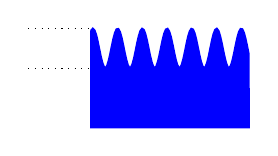
\begin{tikzpicture}
\YEaaxis{1}{4}{1}{2}
\draw[thick, blue, fill] plot[domain=1:3, samples=100] (\x,{.25*sin(20*\x r)+1})--(3,0)--(1,0)--(1,1.23);
\YExcoord{1}{1};
\YExcoord{3}{3};
\YEycoord{0.75}{0.75};
\YEycoord{1.25}{1.25};
\foreach \x in {0.75,1.25}{\draw[dotted] (.2,\x)--(1,\x);}
\end{tikzpicture}
\end{center}
\end{question}
\begin{hint}
Draw a rectangle that \emph{encompasses} the entire shaded area, and one that is \emph{encompassed by} the shaded area. The shaded area is no more than the area of the bigger rectangle, and no less than the area of the smaller rectangle.
\end{hint}
\begin{answer}
The area is between $1.5$ and $2.5$ square units.
\end{answer}
\begin{solution}
\begin{center}
\begin{tikzpicture}
\YEaaxis{1}{4}{1}{2}
\draw[thick, blue, fill] plot[domain=1:3, samples=100] (\x,{.25*sin(20*\x r)+1})--(3,0)--(1,0)--(1,1.23);
\YExcoord{1}{1};
\YExcoord{3}{3};
\YEycoord{0.75}{0.75};
\YEycoord{1.25}{1.25};
\foreach \x in {0.75,1.25}{\draw[dotted] (.2,\x)--(1,\x);}
\draw[red, pattern=crosshatch, pattern color=red] (1,1.25)--(3,1.25)--(3,0)--(1,0)--cycle;
\end{tikzpicture}
\qquad
\begin{tikzpicture}
\YEaaxis{1}{4}{1}{2}
\draw[thick, blue, fill] plot[domain=1:3, samples=100] (\x,{.25*sin(20*\x r)+1})--(3,0)--(1,0)--(1,1.23);
\YExcoord{1}{1};
\YExcoord{3}{3};
\YEycoord{0.75}{0.75};
\YEycoord{1.25}{1.25};
\foreach \x in {0.75,1.25}{\draw[dotted] (.2,\x)--(1,\x);}
\draw[red, pattern=crosshatch, pattern color=red] (1,0.75)--(3,0.75)--(3,0)--(1,0)--cycle;
\end{tikzpicture}
\end{center}
The diagram on the left shows a rectangle with area $2 \times 1.25=2.5$ square  units. Since the blue-shaded region is entirely inside this rectangle, the area of the blue-shaded region is no more than 2.5 square units.

The diagram on the right shows a rectangle with area $2 \times 0.75=1.5$ square  units. Since the blue-shaded region contains this entire rectangle, the area of the blue region is no less than 1.5 square units.

So, the area of the blue-shaded region is between 1.5 and 2.5 square units.

Remark: we could also give an obvious range, like ``the shaded area is between zero and one million square units." This would be true, but not very useful or interesting.
\end{solution}


\begin{Mquestion}
Give a range of possible values for the shaded area in the picture below.
\begin{center}
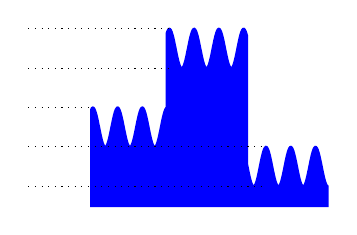
\begin{tikzpicture}
\YEaaxis{1.5}{5}{1}{3}
\draw[thick, blue, fill] plot[domain=1:1.96, samples=100] (\x,{.25*sin(20*\x r)+1})--
plot[domain=1.96:2.98, samples=100] (\x,{.25*sin(20*(\x-1.6) r )+2})--
plot[domain=2.98:4, samples=100] (\x,{.25*sin(20*\x r)+.5})--(4,0)--(1,0)--(1,1.23);
\YExcoord{1}{1};
\YExcoord{1.96}{2};
\YExcoord{2.98}{3};
\YExcoord{4}{4};

\YEycoord{0.75}{0.75};
\YEycoord{1.25}{1.25};
\YEycoord{0.25}{0.25};
\YEycoord{2.25}{2.25};
\YEycoord{1.75}{1.75};

\foreach \x in {0.75, 0.25}{\draw[dotted] (.2,\x)--(3.2,\x);}
\foreach \x in {1.75,2.25}{\draw[dotted] (.2,\x)--(2,\x);}
\foreach \x in {1.25}{\draw[dotted] (.2,\x)--(1,\x);}

\end{tikzpicture}
\end{center}
\end{Mquestion}
\begin{hint}
We can improve on the method of Question~\ref{concept_int_a} by using three rectangles that together encompass the shaded region, and three rectangles that together are encompassed by the shaded region.
\end{hint}
\begin{answer}
The shaded area is between 2.75 and 4.25 square units. (Other estimates are possible, but this is a reasonable estimate, using methods from this chapter.)
\end{answer}
\begin{solution}

\begin{description}
\item[Solution 1:]
One naive way to solve this is to simply use the same method as Question~\ref{concept_int_a}.

\begin{center}
\begin{tikzpicture}
\YEaaxis{1.5}{5}{1}{3}
\draw[thick, blue, fill] plot[domain=1:1.96, samples=100] (\x,{.25*sin(20*\x r)+1})--
plot[domain=1.96:2.98, samples=100] (\x,{.25*sin(20*(\x-1.6) r )+2})--
plot[domain=2.98:4, samples=100] (\x,{.25*sin(20*\x r)+.5})--(4,0)--(1,0)--(1,1.23);
\YExcoord{1}{1};
\YExcoord{1.96}{2};
\YExcoord{2.98}{3};
\YExcoord{4}{4};

\YEycoord{0.75}{0.75};
\YEycoord{1.25}{1.25};
\YEycoord{0.25}{0.25};
\YEycoord{2.25}{2.25};
\YEycoord{1.75}{1.75};
\draw[dotted] (.2,2.25)--(1,2.25);
\draw[red, pattern=crosshatch, pattern color=red] (1,2.25)--(4,2.25)--(4,0)--(1,0)--cycle;
\end{tikzpicture}
\qquad
\begin{tikzpicture}
\YEaaxis{1.5}{5}{1}{3}
\draw[thick, blue, fill] plot[domain=1:1.96, samples=100] (\x,{.25*sin(20*\x r)+1})--
plot[domain=1.96:2.98, samples=100] (\x,{.25*sin(20*(\x-1.6) r )+2})--
plot[domain=2.98:4, samples=100] (\x,{.25*sin(20*\x r)+.5})--(4,0)--(1,0)--(1,1.23);
\YExcoord{1}{1};
\YExcoord{1.96}{2};
\YExcoord{2.98}{3};
\YExcoord{4}{4};

\YEycoord{0.75}{0.75};
\YEycoord{1.25}{1.25};
\YEycoord{0.25}{0.25};
\YEycoord{2.25}{2.25};
\YEycoord{1.75}{1.75};
\draw[dotted] (.2,.25)--(1,.25);
\draw[red, pattern=crosshatch, pattern color=red] (1,0.25)--(4,0.25)--(4,0)--(1,0)--cycle;
\end{tikzpicture}
\end{center}
 The rectangle on the left has area $3 \times 2.25 = 6.75$ square units, and encompasses the entire shaded region.
  The rectangle on the right has area $3 \times 0.25 = 0.75$ square units, and is entirely contained inside the blue-shaded region. So, the area of the blue-shaded region is between 0.75 and 6.75 square units.

 This is a legitimate approximation, but we can easily do much better. The shape of this graph suggests that using the areas of \emph{three} rectangles would be a natural way to improve our estimate.
 \item[Solution 2:]
Let's use these rectangles instead:
\begin{center}
\begin{tikzpicture}
\YEaaxis{1}{5}{1}{3}
\draw[thick, blue, fill] plot[domain=1:1.96, samples=100] (\x,{.25*sin(20*\x r)+1})--
plot[domain=1.96:2.98, samples=100] (\x,{.25*sin(20*(\x-1.6) r )+2})--
plot[domain=2.98:4, samples=100] (\x,{.25*sin(20*\x r)+.5})--(4,0)--(1,0)--(1,1.23);
\YExcoord{1}{1};
\YExcoord{1.96}{2};
\YExcoord{2.98}{3};
\YExcoord{4}{4};

\YEycoord{0.75}{0.75};
\YEycoord{1.25}{1.25};
\YEycoord{0.25}{0.25};
\YEycoord{2.25}{2.25};
\YEycoord{1.75}{1.75};

\foreach \x in {0.75, 0.25}{\draw[dotted] (.2,\x)--(3.2,\x);}
\foreach \x in {1.75,2.25}{\draw[dotted] (.2,\x)--(2,\x);}
\foreach \x in {1.25}{\draw[dotted] (.2,\x)--(1,\x);}


\draw[red, pattern=crosshatch, pattern color=red] (1,1.25)-| (2,2.25)-|(3,0.75)-|(4,0)--(1,0)--cycle;
\end{tikzpicture}
\qquad
\begin{tikzpicture}
\YEaaxis{1}{5}{1}{3}
\draw[thick, blue, fill] plot[domain=1:1.96, samples=100] (\x,{.25*sin(20*\x r)+1})--
plot[domain=1.96:2.98, samples=100] (\x,{.25*sin(20*(\x-1.6) r )+2})--
plot[domain=2.98:4, samples=100] (\x,{.25*sin(20*\x r)+.5})--(4,0)--(1,0)--(1,1.23);
\YExcoord{1}{1};
\YExcoord{1.96}{2};
\YExcoord{2.98}{3};
\YExcoord{4}{4};

\YEycoord{0.75}{0.75};
\YEycoord{1.25}{1.25};
\YEycoord{0.25}{0.25};
\YEycoord{2.25}{2.25};
\YEycoord{1.75}{1.75};

\foreach \x in {0.75, 0.25}{\draw[dotted] (.2,\x)--(3.2,\x);}
\foreach \x in {1.75,2.25}{\draw[dotted] (.2,\x)--(2,\x);}
\foreach \x in {1.25}{\draw[dotted] (.2,\x)--(1,\x);}


\draw[red, pattern=crosshatch, pattern color=red] (1,0.75)-| (2,1.75)-|(3,0.25)-|(4,0)--(1,0)--cycle;
\end{tikzpicture}
\end{center}
In the left picture, the red area is $(1 \times 1.25)+(1 \times 2.25)+(1 \times 0.75)=4.25$ square units. In the right picture, the red area is $(1 \times 0.75)+(1 \times 1.75)+(1 \times 0.25)=2.75$ square units. So, the blue shaded area is between 2.75 and 4.25 square units.
 \end{description}
\end{solution}

\begin{question}
Using rectangles, find a lower and upper bound for $\displaystyle\int_1^3 \dfrac{1}{2^x}\dee{x}$ that differ by at most 0.2 square units.
\begin{center}
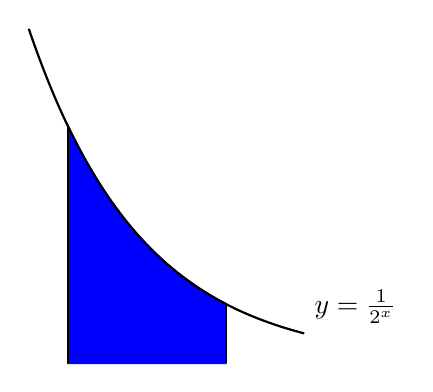
\begin{tikzpicture}
\YEaaxis{1}{5}{1}{5}
\draw[thick, blue, fill] plot[domain=1:3, samples=100] (\x,{6*pow(.5,\x)})--(3,0)--(1,0)--cycle;
\draw[thick] plot[domain=0.5:4, samples=100] (\x,{6*pow(.5,\x)}) node[above right]{$y=\frac{1}{2^x}$};
\YExcoord{1}{1};
\YExcoord{3}{3};
\draw[thick] (1,0)--(1,3) (3,0)--(3,.75);
\end{tikzpicture}
\end{center}
\end{question}
\begin{hint}
Four rectangles suffice.
\end{hint}
\begin{answer}
The area under the curve is a number in the interval $\left( \frac{3}{8}\left[\frac{1}{2}+\frac{1}{\sqrt{2}}\right], \frac{3}{8}\left[1+\frac{1}{\sqrt{2}}\right]\right)$.
\end{answer}
\begin{solution}
Remark: in the solution below, we find the appropriate approximation using trial and error. In Question~\ref{1.1errornotaylor}, we take a more systematic approach.
\begin{description}
\item[Try 1:] First, we can try by using a single rectangle as an overestimate, and a single rectangle as an underestimate.

\begin{center}
\begin{tikzpicture}
\YEaaxis{1}{5}{1}{5}
\draw[thick, blue, fill] plot[domain=1:3, samples=100] (\x,{6*pow(.5,\x)})--(3,0)--(1,0)--cycle;
\draw[thick] plot[domain=0.5:4, samples=100] (\x,{6*pow(.5,\x)}) node[above right]{$y=\frac{1}{2^x}$};
\YExcoord{1}{1};
\YExcoord{3}{3};
\YEycoord{3}{1/2};
\YEycoord{0.75}{1/8};
\draw[red, pattern=crosshatch, pattern color=red] (1,3) rectangle (3,0);
\end{tikzpicture}
\qquad
\begin{tikzpicture}
\YEaaxis{1}{5}{1}{5}
\draw[thick, blue, fill] plot[domain=1:3, samples=100] (\x,{6*pow(.5,\x)})--(3,0)--(1,0)--cycle;
\draw[thick] plot[domain=0.5:4, samples=100] (\x,{6*pow(.5,\x)}) node[above right]{$y=\frac{1}{2^x}$};
\YExcoord{1}{1};
\YExcoord{3}{3};
\YEycoord{3}{1/2};
\YEycoord{0.75}{1/8};
\draw[red, pattern=crosshatch, pattern color=red] (1,0.75) rectangle (3,0);
\end{tikzpicture}
\end{center}

The area under the curve is less than the area of the rectangle on the left ($2 \times \frac{1}{2}=1$) and greater than the area of the rectangle on the right ($2 \times \frac{1}{8}=\frac{1}{4}$). So, the area is in the range $\left(\frac{1}{4},1\right)$. Unfortunately, this range is too big--we need our range to have length at most 0.2. So, we refine our approximation by using more rectangles.

\item[Try 2:] Let's try using two rectangles each for the upper and lower bounds.

\begin{center}
\begin{tikzpicture}
\YEaaxis{1}{5}{1}{5}
\draw[thick, blue, fill] plot[domain=1:3, samples=100] (\x,{6*pow(.5,\x)})--(3,0)--(1,0)--cycle;
\draw[thick] plot[domain=0.5:4, samples=100] (\x,{6*pow(.5,\x)}) node[above right]{$y=\frac{1}{2^x}$};
\YExcoord{1}{1};
\YExcoord{2}{2};
\YExcoord{3}{3};
\YEycoord{3}{1/2};
\YEycoord{1.5}{1/4};
\YEycoord{0.75}{1/8};
\draw[red, pattern=crosshatch, pattern color=red] (1,3) rectangle (2,0) (2,1.5) rectangle (3,0);
\end{tikzpicture}
\qquad
\begin{tikzpicture}
\YEaaxis{1}{5}{1}{5}
\draw[thick, blue, fill] plot[domain=1:3, samples=100] (\x,{6*pow(.5,\x)})--(3,0)--(1,0)--cycle;
\draw[thick] plot[domain=0.5:4, samples=100] (\x,{6*pow(.5,\x)}) node[above right]{$y=\frac{1}{2^x}$};
\YExcoord{1}{1};
\YExcoord{3}{3};
\YExcoord{2}{2};
\YEycoord{3}{1/2};
\YEycoord{1.5}{1/4};
\YEycoord{0.75}{1/8};
\draw[red, pattern=crosshatch, pattern color=red] (2,0.75) rectangle (3,0) (1,1.5)rectangle(2,0);
\end{tikzpicture}
\end{center}

The rectangles in the left picture have area
$\left(1 \times \frac{1}{2}\right)+\left(1 \times \frac{1}{4}\right)=\frac{3}{4}$, and the rectangles in the right picture have area
$\left(1 \times \frac{1}{4}\right)+\left(1 \times \frac{1}{8}\right)=\frac{3}{8}$. So, the area under the curve is in the interval $\left(\frac{3}{8},\frac{3}{4}\right)$. The length of this interval is $\frac{3}{8}$, and $\frac{3}{8}>\frac{3}{15}=\frac{1}{5}=0.2$. (Indeed, $\frac{3}{8}=0.375>0.2$.) Since the length of our interval is still bigger than 0.2,  we need even more rectangles.
\item[Try 3:]
Let's go ahead and try four rectangles each for the upper and lower estimates.

\begin{center}
\begin{tikzpicture}[scale=0.85]
\YEaaxis{1}{5}{1}{5}
\draw[thick, blue, fill] plot[domain=1:3, samples=100] (\x,{6*pow(.5,\x)})--(3,0)--(1,0)--cycle;
\draw[thick] plot[domain=0.5:4, samples=100] (\x,{6*pow(.5,\x)}) node[above right]{$y=\frac{1}{2^x}$};
\YExcoord{1}{1};
\YExcoord{2}{2};
\YExcoord{3}{3};
\YEycoord{3}{1/2};
%\YEycoord{2.12}{1/(2\sqrt{2})};
\YEycoord{1.5}{1/4};
\draw (0.2,1.06)--(-1,1.06) node[left]{$1/(4\sqrt{2})$};
\draw (0.2,2.12)--(-1,2.12) node[left]{$1/(2\sqrt{2})$};
\YEycoord{0.75}{1/8};
\draw[red, pattern=crosshatch, pattern color=red] (1,3) rectangle (1.5,0) (1.5,2.12)rectangle(2,0)
(2,1.5)rectangle(2.5,0)
(2.5,1.06)rectangle(3,0);
\end{tikzpicture}
\hfill
\begin{tikzpicture}[scale=0.85]
\YEaaxis{1}{5}{1}{5}
\draw[thick, blue, fill] plot[domain=1:3, samples=100] (\x,{6*pow(.5,\x)})--(3,0)--(1,0)--cycle;
\draw[thick] plot[domain=0.5:4, samples=100] (\x,{6*pow(.5,\x)}) node[above right]{$y=\frac{1}{2^x}$};
\YExcoord{1}{1};
\YExcoord{2}{2};
\YExcoord{3}{3};
\YEycoord{3}{1/2};
%\YEycoord{2.12}{1/(2\sqrt{2})};
\YEycoord{1.5}{1/4};
\draw (0.2,1.06)--(-1,1.06) node[left]{$1/(4\sqrt{2})$};
\draw (0.2,2.12)--(-1,2.12) node[left]{$1/(2\sqrt{2})$};
\YEycoord{0.75}{1/8};

\draw[red, pattern=crosshatch, pattern color=red] (1,2.12)rectangle(1.5,0)
(1.5,1.5)rectangle(2,0)
(2,1.06)rectangle(2.5,0)
(2.5,0.75) rectangle (3,0);
\end{tikzpicture}
\end{center}

The area of the rectangles on the left is:
\[\left(\frac{1}{2}\times \frac{1}{2}\right)+
\left(\frac{1}{2}\times \frac{1}{2\sqrt{2}}\right)+
\left(\frac{1}{2}\times \frac{1}{4}\right)+
\left(\frac{1}{2}\times \frac{1}{4\sqrt{2}}\right) = \frac{3}{8}\left[1+\frac{1}{\sqrt{2}}\right],\] and the area of the rectangles on the right is:
\[\left(\frac{1}{2}\times \frac{1}{2\sqrt{2}}\right)+
\left(\frac{1}{2}\times \frac{1}{4}\right)+
\left(\frac{1}{2}\times \frac{1}{4\sqrt{2}}\right)+
\left(\frac{1}{2}\times \frac{1}{8}\right) = \frac{3}{8}\left[\frac{1}{2}+\frac{1}{\sqrt{2}}\right].\] So, the area under the curve is in the interval $\left( \frac{3}{8}\left[\frac{1}{2}+\frac{1}{\sqrt{2}}\right], \frac{3}{8}\left[1+\frac{1}{\sqrt{2}}\right]\right)$. The length of this interval is $\frac{3}{16}$, and $\frac{3}{16}<\frac{3}{15}=\frac{1}{5}=0.2$, as desired. (Indeed, $\frac{3}{16}=0.1875<0.2$.)

Note, if we choose any value in the interval $\left( \frac{3}{8}\left[\frac{1}{2}+\frac{1}{\sqrt{2}}\right], \frac{3}{8}\left[1+\frac{1}{\sqrt{2}}\right]\right)$ as an approximation for the area under the curve, our error is no more than 0.2.
\end{description}
\end{solution}

\begin{Mquestion}
Let $f(x)$ be a function that is \emph{decreasing} from $x=0$ to $x=5$. Which Riemann sum approximation of $\displaystyle\int_0^5 f(x)\dee{x}$ is the largest--left, right, or midpoint?
\end{Mquestion}
\begin{hint}
Try drawing a picture.
\end{hint}
\begin{answer}
left
\end{answer}
\begin{solution}
Since $f(x)$ is decreasing, it is larger on the left endpoint of an interval than on the right endpoint of an interval. So, a \emph{left} Riemann sum gives a larger approximation. Notice this does not depend on $n$.

Furthermore, the actual area $\displaystyle\int_0^5f(x)\dee{x}$ is larger than its right Riemann sum, and smaller than its left Riemann sum.

\begin{center}
\begin{tikzpicture}[scale=0.85]
\YEaaxis{1}{5}{1}{5}
\draw[thick, blue, fill] plot[domain=1:3, samples=100] (\x,{6*pow(.5,\x)})--(3,0)--(1,0)--cycle;
\draw[thick] plot[domain=0.5:4, samples=100] (\x,{6*pow(.5,\x)}) ;
\draw[red, pattern=crosshatch, pattern color=red] (1,3) rectangle (1.5,0) (1.5,2.12)rectangle(2,0)
(2,1.5)rectangle(2.5,0)
(2.5,1.06)rectangle(3,0);
\draw (1,-.5) node[below right]{left Riemann sum};
\end{tikzpicture}
\hspace{1cm}
\begin{tikzpicture}[scale=0.85]
\YEaaxis{1}{5}{1}{5}
\draw[thick, blue, fill] plot[domain=1:3, samples=100] (\x,{6*pow(.5,\x)})--(3,0)--(1,0)--cycle;
\draw[thick] plot[domain=0.5:4, samples=100] (\x,{6*pow(.5,\x)}) ;
\draw[red, pattern=crosshatch, pattern color=red] (1,2.12)rectangle(1.5,0)
(1.5,1.5)rectangle(2,0)
(2,1.06)rectangle(2.5,0)
(2.5,0.75) rectangle (3,0);
\draw (1,-.5) node[below right]{right Riemann sum};
\end{tikzpicture}

\end{center}
\end{solution}

\begin{question}\label{concept_int_b}
Give an example of a function $f(x)$, an interval $[a,b]$, and a number $n$ such that the midpoint Riemann sum of $f(x)$ over $[a,b]$ using $n$ intervals is \emph{larger than} both the left and right Riemann sums  of $f(x)$ over $[a,b]$ using $n$ intervals. %Can you think of several different examples?
\end{question}
\begin{hint}
Try an oscillating function.
\end{hint}
\begin{answer}
Many answers are possible. One example is $f(x)=\sin x$, $[a,b]=[0,\pi]$, $n=1$.
Another example is $f(x)=\sin x$, $[a,b]=[0,5\pi]$, $n=5$.
\end{answer}
\begin{solution}
If $f(x)$ is always increasing or always decreasing, then the midpoint Riemann sum will be between the left and right Riemann sums. So, we need a function that goes up and down. Many examples are possible, but let's work with a familiar one: $\sin x$.

If our intervals have endpoints that are integer multiples of $\pi$, then the left and right Riemann sums will be 0, since $\sin(0)=\sin(\pi)=\sin(2\pi)=\cdots=0$. The midpoints of these intervals will give $y$-values of 1 and -1. So, for example, we can let $f(x)=\sin x$, $[a,b]=[0,\pi]$, and $n=1$. Then the right and left Riemann sums are 0, while the midpoint Riemann sum is $\pi$.

We can extend the example of $f(x)=\sin x$ to have more intervals. As long as we have more positive terms than negative,  the midpoint approximation will be a positive number, and so it will be larger than both the left and right Riemann sums. So, for example, we can let $f(x)=\sin x$, $[a,b]=[0,5\pi]$, and $n=5$. Then the midpoint Riemann sum is $\pi-\pi+\pi-\pi+\pi=\pi$, which is strictly larger than 0 and so it is larger than both the left and right Riemann sums.

\begin{center}
\begin{tikzpicture}
\YEaaxis{1}{6}{2}{2}
\draw[thick] plot[domain=-.5:5.08, samples=60] (\x,{1.5*sin(\x*3.14 r) });
\foreach \x in {0,2,4}{
	\ADD{\x}{1}{\y}
	\ADD{\x}{.5}{\z}
	\draw[fill=blue, fill opacity=0.5] (\x,0) rectangle (\y,1.5);
	\draw[blue, thick, dashed, blue] (\z,0)--(\z,1.5);}
\foreach \x in {1,3}{
	\ADD{\x}{1}{\y}
	\draw[red, fill=red, fill opacity=0.5] (\x,0) rectangle (\y,-1.5);
	\ADD{\x}{.5}{\z}
	\draw[thick, dashed, red] (\z,0)--(\z,-1.5);}
\YExcoord{5}{5\pi}
\end{tikzpicture}
\end{center}
\end{solution}

\Instructions{In Questions~\ref{1.1sigmaa} through \ref{1.1sigmab}, we practice using sigma notation. There are many ways to write a given sum in sigma notation. You can practice finding several, and deciding which looks the clearest.}
\begin{question}\label{1.1sigmaa}
Express the following sums in sigma notation:
\begin{enumerate}[(a)]
\item $3+4+5+6+7$
\item $6+8+10+12+14$
\item $7+9+11+13+15$
\item $1+3+5+7+9+11+13+15$
\end{enumerate}
\end{question}
\begin{hint} The ordering of the parts is intentional: each sum can be written by changing some small part of the sum before it.
\end{hint}
\begin{answer} Some of the possible answers are given, but more exist.
\begin{enumerate}[(a)]
\item $\displaystyle\sum_{i=3}^7 i$\quad;\quad $\displaystyle\sum_{i=1}^5 (i+2)$
\item $\displaystyle\sum_{i=3}^7 2i$\quad;\quad $\displaystyle\sum_{i=1}^5 (2i+4)$
\item $\displaystyle\sum_{i=3}^7 (2i+1)$\quad;\quad $\displaystyle\sum_{i=1}^5 (2i+5)$
\item $\displaystyle\sum_{i=1}^8 (2i-1)$\quad;\quad$\displaystyle\sum_{i=0}^7 (2i+1)$
\end{enumerate}
\end{answer}
\begin{solution}
\begin{enumerate}[(a)]
\item Two possible answers are $\displaystyle\sum_{i=3}^7 i$ and $\displaystyle\sum_{i=1}^5 (i+2)$. The first has simpler terms ($i$ versus $i+2$), while the second has simpler indices (we often like to start at $i=1$). Neither is objectively better than the other, but  depending on your purposes you might find one more useful.
\item The terms of this sum are each double the terms of the sum from part (a), so two possible answers are $\displaystyle\sum_{i=3}^7 2i$ and $\displaystyle\sum_{i=1}^5 (2i+4)$. \\
We often want to write a sum that involves even numbers: it will be useful for you to remember that the term  $2i$ (with index $i$) generates evens.
\item\label{1.1sigma1c} The terms of this sum are each one more than the terms of the  sum from part (b), so two possible answers are $\displaystyle\sum_{i=3}^7 (2i+1)$ and $\displaystyle\sum_{i=1}^5 (2i+5)$. \\
In the last part, we used the expression $2i$ to generate even numbers; $2i+1$ will generate odds. So will the index $2i+5$, and indeed, $2i+k$ for any odd number $k$. The choice of what you add will depend on the bounds of $i$.
\item This sum adds up the odd numbers from 1 to 15. From  Part~(\ref{1.1sigma1c}), we know that the formula $2i+1$ is a simple way of generating odd numbers. Since our first term should be 1 and our last term should be 15, if we use $\sum (2i+1)$, then $i$ should run from $0$ to $7$. So, one way of expressing our sum in sigma notation is $\displaystyle\sum_{i=0}^7 (2i+1)$.

Sometimes we like our sum to start at $i=1$ instead of $i=0$. If this is our desire, we can use $2i-1$ as our terms, and let $i$ run from 1 to 8. This gives us another way of expressing our sum:
 $\displaystyle\sum_{i=1}^8 (2i-1)$.
\end{enumerate}
\end{solution}

\begin{Mquestion}\label{1.1powers}
Express the following sums in sigma notation:
\begin{enumerate}[(a)]
\item $\frac{1}{3}+\frac{1}{9}+\frac{1}{27}+\frac{1}{81}$
\item $\frac{2}{3}+\frac{2}{9}+\frac{2}{27}+\frac{2}{81}$
\item $-\frac{2}{3}+\frac{2}{9}-\frac{2}{27}+\frac{2}{81}$
\item $\frac{2}{3}-\frac{2}{9}+\frac{2}{27}-\frac{2}{81}$
\end{enumerate}
\end{Mquestion}
\begin{hint} If we raise $-1$ to an even power, we get $+1$, and if we raise it to an odd power, we get $-1$.
\end{hint}
\begin{answer} Some answers are below, but others are possible.
\begin{enumerate}[(a)]
\item $\displaystyle\sum_{i=1}^4 \frac{1}{3^i}$\quad;\quad
$\displaystyle\sum_{i=1}^4 \left(\frac{1}{3}\right)^i$
\item $\displaystyle\sum_{i=1}^4 \frac{2}{3^i}$\quad;\quad $\displaystyle\sum_{i=1}^4 2\left(\frac{1}{3}\right)^i$
\item $\displaystyle\sum_{i=1}^4(-1)^i \frac{2}{3^i}$
\quad;\quad
$\displaystyle\sum_{i=1}^4  \frac{2}{(-3)^i}$
\item $\displaystyle\sum_{i=1}^4(-1)^{i+1} \frac{2}{3^i}$
\quad;\quad
$\displaystyle\sum_{i=1}^4  -\frac{2}{(-3)^i}$
\end{enumerate}
\end{answer}
\begin{solution}
\begin{enumerate}[(a)]
\item The denominators are successive powers of three, so one way of writing this is $\displaystyle\sum_{i=1}^4 \frac{1}{3^i}$. Equivalently, the terms we're adding are powers of $1/3$, so we can also write
$\displaystyle\sum_{i=1}^4 \left(\frac{1}{3}\right)^i$.
\item This sum is obtained from the sum in (a) by multiplying each term by two, so we can write $\displaystyle\sum_{i=1}^4 \frac{2}{3^i}$ or $\displaystyle\sum_{i=1}^4 2\left(\frac{1}{3}\right)^i$.
\item The difference between this sum and the previous sum is its alternating sign, minus-plus-minus-plus. This behaviour appears when we raise a negative number to successive powers. We can multiply each term by $(-1)^i$, or we can slip a negative into the number that is already raised to the power $i$: $\displaystyle\sum_{i=1}^4(-1)^i \frac{2}{3^i}$\,, or
$\displaystyle\sum_{i=1}^4  \frac{2}{(-3)^i}$.
\item This sum is the negative of the sum in part (c), so we can simply multiply each term by negative one: $\displaystyle\sum_{i=1}^4(-1)^{i+1} \frac{2}{3^i}$
\,, or $\displaystyle\sum_{i=1}^4  -\frac{2}{(-3)^i}$\,.

Be careful with the second form: a common mistake is to think that $-\dfrac{2}{(-3)^i} = \dfrac{2}{3^i}$, but these are not the same.
\end{enumerate}
\end{solution}

\begin{question}
Express the following sums in sigma notation:
\begin{enumerate}[(a)]
\item $\frac{1}{3}+\frac{1}{3}+\frac{5}{27}+\frac{7}{81}+\frac{9}{243}$
\item $\frac{1}{5}+\frac{1}{11}+\frac{1}{29}+\frac{1}{83}+\frac{1}{245}$
\item $1000+200+30+4+\frac{1}{2}+\frac{3}{50}+\frac{7}{1000}$
\end{enumerate}
\end{question}
\begin{hint}
Sometimes a little anti-simplification can make the pattern more clear.
\begin{enumerate}[(a)]
\item Re-write as $\frac{1}{3}+\frac{3}{9}+\frac{5}{27}+\frac{7}{81}+\frac{9}{243}$.
\item Compare to the sum in the hint for (a).
\item Re-write as $1\cdot1000+2\cdot 100+3\cdot10+\frac{4}{1}+\frac{5}{10}+\frac{6}{100}+\frac{7}{1000}$.
\end{enumerate}
\end{hint}
\begin{answer}
\begin{enumerate}[(a)]
\item $\displaystyle\sum_{i=1}^5 \frac{2i-1}{3^i}$
\item $\displaystyle\sum_{i=1}^5 \frac{1}{3^i+2}$
\item $\displaystyle\sum_{i=1}^7 i\cdot10^{4-i}$\quad;\quad $\displaystyle\sum_{i=1}^7 \frac{i}{10^{i-4}}$
\end{enumerate}
\end{answer}
\begin{solution}
\begin{enumerate}[(a)]
\item If we re-write the second term as $\frac{3}{9}$ instead of $\frac{1}{3}$, our sum becomes:
\[\frac{1}{3}+\frac{3}{9}+\frac{5}{27}+\frac{7}{81}+\frac{9}{243}\]
The numerators are the first five odd numbers, and the denominators are the first five positive powers of 3. We learned how to generate odd numbers in Question~\ref{1.1sigmaa}, and we learned how to generate powers of three in Question~\ref{1.1powers}. Combining these, we can write our sum as
$\displaystyle\sum_{i=1}^5 \frac{2i-1}{3^i}$\,.
\item The denominators of these terms differ from the denominators of part (a) by precisely two, while the numerators are simply 1. So, we can modify our previous answer: $\displaystyle\sum_{i=1}^5 \frac{1}{3^i+2}$\,.
\item Let's re-write the sum to make the pattern clearer.
\end{enumerate}
\[\begin{array}{cccccccccccccc}
&1000&+&200&+&30&+&4&+&\frac{1}{2}&+&\frac{3}{50}&+&\frac{7}{1000}\\[5pt]
=&1\cdot1000&+&2\cdot 100&+&3\cdot10&+&\frac{4}{1}&+&\frac{5}{10}&+&\frac{6}{100}&+&\frac{7}{1000}\\[5pt]
=&1\cdot 10^3 &+& 2\cdot 10^2&+&3\cdot 10^1 &+& 4\cdot 10^0 &+& 5 \cdot 10^{-1} &+&
6\cdot 10^{-2} &+& 7 \cdot 10^{-3} \\[5pt]
=&\textcolor{red}1\cdot 10^{4-\textcolor{red}1} &+& \textcolor{red}2\cdot 10^{4-\textcolor{red}2}&+&\textcolor{red}3\cdot 10^{4-\textcolor{red}3} &+& \textcolor{red}4\cdot 10^{4-\textcolor{red}4} &+& \textcolor{red}5 \cdot 10^{4-\textcolor{red}5} &+&
\textcolor{red}6\cdot 10^{4-\textcolor{red}6} &+& \textcolor{red}7 \cdot 10^{4-\textcolor{red}7}
\end{array}\]
If we let the red numbers be our index $i$, this gives us the expression $\displaystyle\sum_{i=1}^7 i\cdot10^{4-i}$\,. Equivalently, we can write $\displaystyle\sum_{i=1}^7 \frac{i}{10^{i-4}}$\,.

\end{solution}

\begin{question}
Evaluate the following sums. You might want to use the formulas from Theorems ~\eref{CLP101}{thm:INTsummationArith} and \eref{CLP101}{thm:INTspecialSums}
in the CLP-2 text.
\begin{enumerate}[(a)]
\item $\displaystyle\sum_{i=0}^{100} \left(\dfrac{3}{5}\right)^i$
\item $\displaystyle\sum_{i=50}^{100} \left(\dfrac{3}{5}\right)^i$
\item $\displaystyle\sum_{i=1}^{10} \left(i^2-3i+5\right)$
\item $\displaystyle\sum_{n=1}^{b}\left[ \left(\frac{1}{e}\right)^n+en^3\right]$, where $b$ is some integer greater than 1.
\end{enumerate}
\end{question}
\begin{hint}
(a), (b) These are geometric sums.\\
(c) You can write this as three separate sums.\\
(d) You can write this as two separate sums. Remember that $e$ is a constant.  Don't be thrown off by the index being $n$ instead of $i$.
\end{hint}
\begin{answer}
\begin{enumerate}[(a)]
\item $\dfrac{5}{2}\left[1-\left(\dfrac{3}{5}\right)^{101}\right]$
\item $\dfrac{5}{2}\left(\dfrac{3}{5}\right)^{50}\left[1-\left(\dfrac{3}{5}\right)^{51}\right]$
\item $270$
\item $\dfrac{1-\left(\frac{1}{e}\right)^b}{e-1}+\dfrac{e}{4}\left[b(b+1)\right]^2$
\end{enumerate}
\end{answer}
\begin{solution}
\begin{enumerate}[(a)]
\item Using Theorem~\eref{CLP101}{thm:INTspecialSums}.a in the CLP-2 text,
with $a=1$, $r=\frac{3}{5}$ and $n=100$:
\[\sum_{i=0}^{100} \left(\dfrac{3}{5}\right)^i = \dfrac{1-\left(\frac{3}{5}\right)^{101}}{1-\frac{3}{5}} = \dfrac{5}{2}\left[1-\left(\frac{3}{5}\right)^{101}\right]\]
\item We want to use Theorem~\eref{CLP101}{thm:INTspecialSums}, part (a) again, but our sum doesn't start at $\left(\frac{3}{5}\right)^0=1$. We have two options: factor out the leading term, or use the difference of two sums that start where we want them to.
\begin{description}
\item[Solution 1:] In this solution, we'll make our sum start at 1 by factoring out the leading term. We wrote our work out the long way (expanding the sigma into ``dot-dot-dot" notation) for clarity, but it's faster to do the algebra in sigma notation all the way through.
\begin{align*}
\displaystyle\sum_{i=50}^{100} \left(\dfrac{3}{5}\right)^i&=
 \left(\dfrac{3}{5}\right)^{50}+ \left(\dfrac{3}{5}\right)^{51}+ \left(\dfrac{3}{5}\right)^{52}+\cdots+ \left(\dfrac{3}{5}\right)^{100}\\
 &=
 \left(\dfrac{3}{5}\right)^{50}\left[1+ \left(\dfrac{3}{5}\right)+ \left(\dfrac{3}{5}\right)^{2}+\cdots+ \left(\dfrac{3}{5}\right)^{50}\right]
\\
&= \left(\dfrac{3}{5}\right)^{50}\dfrac{1-\left(\frac{3}{5}\right)^{51}}{1-\frac{3}{5}}\\
&=\dfrac{5}{2}\left(\dfrac{3}{5}\right)^{50}\left[1-\left(\frac{3}{5}\right)^{51}\right].
\end{align*}

\item[Solution 2:]
In this solution, we write our given expression as the difference of two sums, both starting at $i=0$.
\begin{align*}
\displaystyle\sum_{i=50}^{100} \left(\dfrac{3}{5}\right)^i&=
\displaystyle\sum_{i=0}^{100} \left(\dfrac{3}{5}\right)^i-
\displaystyle\sum_{i=0}^{49} \left(\dfrac{3}{5}\right)^i\\
&=\dfrac{1-\left(\frac{3}{5}\right)^{101}}{1-\frac{3}{5}} -
\dfrac{1-\left(\frac{3}{5}\right)^{50}}{1-\frac{3}{5}} \\
&=\dfrac{5}{2}\left[\left(\frac{3}{5}\right)^{50}-\left(\frac{3}{5}\right)^{101}\right]\\
&=\dfrac{5}{2}\left(\dfrac{3}{5}\right)^{50}\left[1-\left(\frac{3}{5}\right)^{51}\right].
\end{align*}
\end{description}
\item Before we can use the equations in Theorem~\eref{CLP101}{thm:INTspecialSums}, we'll need to do a little simplification.
\begin{align*}
\displaystyle\sum_{i=1}^{10} \left(i^2-3i+5\right)&=
\displaystyle\sum_{i=1}^{10} i^2
+\displaystyle\sum_{i=1}^{10} -3i
+\displaystyle\sum_{i=1}^{10}5\\
&=
\displaystyle\sum_{i=1}^{10} i^2
-3\displaystyle\sum_{i=1}^{10} i
+5\displaystyle\sum_{i=1}^{10}1\\
&=
\frac{1}{6}(10)(11)(21)
-3\left(\frac{1}{2}(10\cdot 11)\right)
+5\cdot 10\\
&=270
\end{align*}
\item As in part (c), we'll simplify first. The first part (shown here in red) is a geometric sum, but it does not start at $1=\left(\frac{1}{e}\right)^0$.
\begin{align*}
\displaystyle\sum_{n=1}^{b}\left[\textcolor{red}{ \left(\frac{1}{e}\right)^n}\textcolor{black}+
\,\textcolor{blue}{en^3}\right]&=
\color{red}\displaystyle\sum_{n=1}^{b} \left(\frac{1}{e}\right)^n\color{black}+\color{blue}
\displaystyle\sum_{n=1}^{b}en^3\\
&=\color{red}
\displaystyle\sum_{n=0}^{b} \left(\frac{1}{e}\right)^{n}-1
\color{black}+
\color{blue}e\displaystyle\sum_{n=1}^{b}n^3\\
&=\color{red}
\dfrac{1-\left(\frac{1}{e}\right)^{b+1}}{1-\frac{1}{e}}-1
\color{black}+
\color{blue}e\left[\frac{1}{2}b(b+1)\right]^2\\
              &=\color{red}
              \dfrac{\frac{1}{e}-\left(\frac{1}{e}\right)^{b+1}}{1-\frac{1}{e}}
              \color{black}+
              \color{blue}e\left[\frac{1}{2}b(b+1)\right]^2\\
&=\textcolor{red}{\dfrac{1-\left(\frac{1}{e}\right)^b}{e-1}}+\textcolor{blue}{\frac{e}{4}\left[b(b+1)\right]^2}
\end{align*}
\end{enumerate}
\end{solution}


\begin{question}\label{1.1sigmab}
Evaluate the following sums. You might want to use the formulas from Theorem~\eref{CLP101}{thm:INTspecialSums} in the CLP-2 text.
\begin{enumerate}[(a)]
\item $\displaystyle\sum_{i=50}^{100} (i-50)+\displaystyle\sum_{i=0}^{50} i$
\item $\displaystyle\sum_{i=10}^{100} \left(i-5\right)^3$
\item $\displaystyle\sum_{n=1}^{11} (-1)^n$
\item $\displaystyle\sum_{n=2}^{11} (-1)^{2n+1}$
\end{enumerate}
\end{question}
\begin{hint}
\begin{enumerate}[(a)]
\item Write out the terms of the two sums.
\item A change of index is an easier option than expanding the cubic.
\item Which terms cancel?
\item Remember $2n+1$ is odd for every integer $n$. The index starts at $n=2$, not $n=1$.
\end{enumerate}
\end{hint}
\begin{answer}
\begin{enumerate}[(a)]
\item $50\cdot 51=2550$
\item $\left[\frac{1}{2}(95)(96)\right]^2-\left[\frac{1}{2}(4)(5)\right]^2$
\item $-1$
\item $-10$
\end{enumerate}
\end{answer}
\begin{solution}
\begin{enumerate}[(a)]
\item The two pieces are very similar, which we can see by changing the index, or expanding them out:
\begin{align*}
\displaystyle\sum_{i=50}^{100} (i-50)+\displaystyle\sum_{i=0}^{50} i&=
\left(0+1+2+\cdots + 50\right)+\left(0+1+2+\cdots + 50\right)\\
&=\left(1+2+\cdots + 50\right)+\left(1+2+\cdots + 50\right)\\
&=2\left(1+2+\cdots + 50\right)\\
&=2\sum_{i=1}^{50} i\\
&= 2\left(\frac{50\cdot 51}{2}\right)=50\cdot 51=2550
\end{align*}
\item If we expand $(i-5)^3 = i^3-15i^2+75i-225$, we can break the sum into four parts, and evaluate each separately. However, it is much simpler to change the index and make the term $(i-5)^3$ into $i^3$.
\begin{align*}\displaystyle\sum_{i=10}^{100} \left(i-5\right)^3&=
5^3+6^3+7^3+\cdots +95^3
\intertext{We have a formula to evaluate the sum of cubes if they start at $1$, so we turn our expression into the difference of two sums starting at 1:}
&=
\left[1^3+2^3+3^3+4^3+5^3+6^3+7^3+\cdots +95^3\right]-
\left[1^3+2^3+3^3+4^3\right]\\
&=\displaystyle\sum_{i=1}^{95} i^3 - \displaystyle\sum_{i=1}^4 i^3\\
&=\left[\frac{1}{2}(95)(96)\right]^2-\left[\frac{1}{2}(4)(5)\right]^2\,.
\end{align*}
\item Notice every two terms cancel with each other, since the sum is $(-1)+(+1)$, etc.
Then the terms $n=1$ through $n=10$ cancel, and we're left only with the final term, $(-1)^{11}=-1$.

Written out more explicitly: \begin{align*}
\displaystyle\sum_{n=1}^{11} (-1)^{n}&=-1+1-1+1-1+1-1+1-1+1-1\\
&=[-1+1]+[-1+1]+[-1+1]+[-1+1]+[-1+1]-1\\
&=0+0+0+0+0-1=-1.
\end{align*}
\item For every integer $n$, $2n+1$ is odd, so $(-1)^{2n+1}=-1$. Then $\displaystyle\sum_{n=2}^{11} (-1)^{2n+1} =\displaystyle\sum_{n=2}^{11} -1 =-10$.
\end{enumerate}

\end{solution}


\Instructions{Questions~\ref{1.1Riemanna} through \ref{1.1Riemannb} are meant to give you practice interpreting the formulas in Definition~\eref{CLP101}{def:INTthreeRiemannSums}
of the CLP-2 text. The formulas might look complicated at first, but if you understand what each piece means, they are easy to learn.}
\begin{Mquestion}\label{1.1Riemanna}
In the picture below, draw in the rectangles whose (signed) area is being computed by the midpoint Riemann sum
$\displaystyle\sum_{i=1}^4 \dfrac{b-a}{4}\cdot f\left(a+\left(i-\frac{1}{2}\right)\dfrac{b-a}{4}\right)$.

\begin{center}
\begin{tikzpicture}
\YEaxis{4}{3};
\YExcoord{2.5}{b}
\YExcoord{-2.5}{a}
\draw[very thick] (-3,-3) .. controls (-1.5,4) and (1,-2) .. (3,3) node[right]{$y=f(x)$};
\end{tikzpicture}
\end{center}
\end{Mquestion}
\begin{hint}
Since the sum adds four pieces, there will be four rectangles. However, one might be extremely small.
\end{hint}
\begin{answer}
\begin{center}
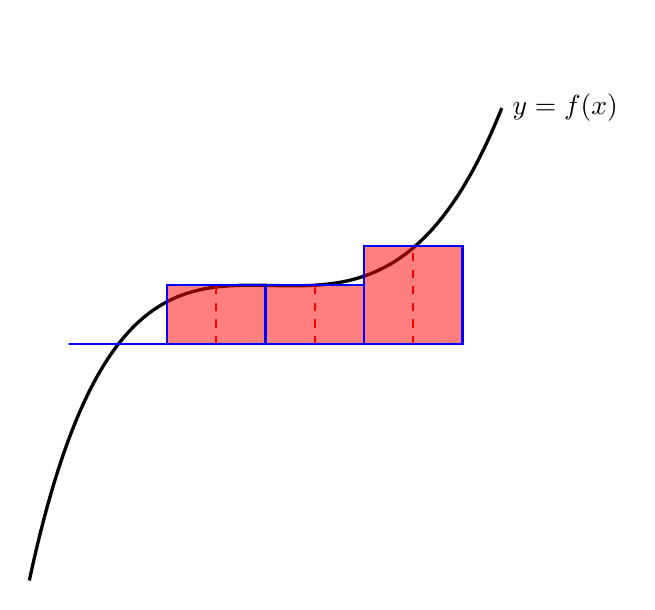
\begin{tikzpicture}
\YEaxis{4}{3};
\YExcoord{2.5}{b}
\YExcoord{-2.5}{a}
\draw[very thick] (-3,-3) .. controls (-1.5,4) and (1,-2) .. (3,3) node[right]{$y=f(x)$};
\draw[thick, red, dashed] (1.875,0)--(1.875,1.25);
\draw[thick, red, dashed] (-0.625,0)--(-0.625,0.75);
\draw[thick, red, dashed] (0.625,0)--(0.625,0.75);
\draw[thick, blue, fill =red, fill opacity=0.5] (-1.25,0) rectangle (0,.75);
\draw[thick, blue, fill =red, fill opacity=0.5] (0,0) rectangle (1.25,.75);
\draw[thick, blue, fill =red, fill opacity=0.5] (1.25,0) rectangle (2.5,1.25);
\draw[thick, blue, fill =red, fill opacity=0.5] (-2.5,0) rectangle (-1.25,0);
\end{tikzpicture}
\end{center}

\end{answer}
\begin{solution}
The index of the sum runs from 1 to 4: the first, second, third, and fourth rectangles. So, we have four rectangles in our Riemann sum. Let's start by drawing in the intervals along the $x$-axis taken up by these four rectangles. Note each has the same width: $\dfrac{b-a}{4}$.
\begin{center}
\begin{tikzpicture}
\YEaxis{4}{3};
\YExcoord{2.5}{b}
\YExcoord{-2.5}{a}
\draw[very thick] (-3,-3) .. controls (-1.5,4) and (1,-2) .. (3,3) node[right]{$y=f(x)$};
\draw[thick, blue] (-2.5,.2)--(-2.5,-.25);
\draw[thick, blue] (-1.25,.2)--(-1.25,-.25);
\draw[thick, blue] (0,.2)--(0,-.25);
\draw[thick, blue] (1.25,.2)--(1.25,-.25);
\draw[thick, blue] (2.5,.2)--(2.5,-.25);
\end{tikzpicture}
\end{center}

Since this is a midpoint Riemann sum, the height of each rectangle is given by the $y$-value of the function in the midpoint of the interval. So, now let's find the height of the function at the midpoints of each of the four intervals.

\begin{center}
\begin{tikzpicture}
\YEaxis{4}{3};
\YExcoord{2.5}{b}
\YExcoord{-2.5}{a}
\draw[very thick] (-3,-3) .. controls (-1.5,4) and (1,-2) .. (3,3) node[right]{$y=f(x)$};
\draw[thick, blue] (-2.5,.2)--(-2.5,-.25);
\draw[thick, blue] (-1.25,.2)--(-1.25,-.25);
\draw[thick, blue] (0,.2)--(0,-.25);
\draw[thick, blue] (1.25,.2)--(1.25,-.25);
\draw[thick, blue] (2.5,.2)--(2.5,-.25);
\draw[thick, red] (-1.875,-.2)--(-1.875,0);
\draw[thick, red] (1.875,-.2)--(1.875,1.25);
\draw[thick, red] (-0.625,-.2)--(-0.625,0.75);
\draw[thick, red] (0.625,-.2)--(0.625,0.75);
\end{tikzpicture}
\end{center}

The left-most interval has a height of about 0, so it gives a ``trivial" rectangle with no height and no area. The middle two intervals have rectangles of about the same height, and the right-most interval has the highest rectangle.

\begin{center}
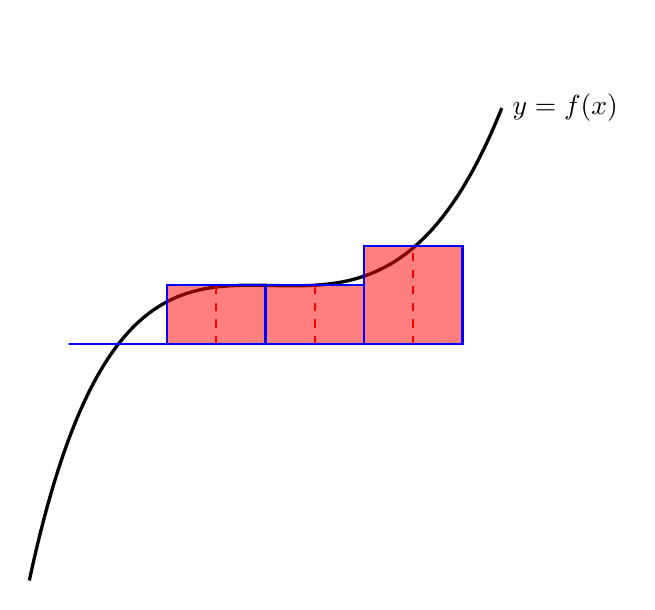
\begin{tikzpicture}
\YEaxis{4}{3};
\YExcoord{2.5}{b}
\YExcoord{-2.5}{a}
\draw[very thick] (-3,-3) .. controls (-1.5,4) and (1,-2) .. (3,3) node[right]{$y=f(x)$};
\draw[thick, red, dashed] (1.875,0)--(1.875,1.25);
\draw[thick, red, dashed] (-0.625,0)--(-0.625,0.75);
\draw[thick, red, dashed] (0.625,0)--(0.625,0.75);
\draw[thick, blue, fill =red, fill opacity=0.5] (-1.25,0) rectangle (0,.75);
\draw[thick, blue, fill =red, fill opacity=0.5] (0,0) rectangle (1.25,.75);
\draw[thick, blue, fill =red, fill opacity=0.5] (1.25,0) rectangle (2.5,1.25);
\draw[thick, blue, fill =red, fill opacity=0.5] (-2.5,0) rectangle (-1.25,0);
\end{tikzpicture}
\end{center}
\end{solution}



%%%%%%%%%%%%%%%%%%%

\begin{question}[M105 2015A]
$\displaystyle \sum_{k=1}^4 f(1+k)\cdot 1$ is a left Riemann sum for a function $f(x)$ on the interval $[a,b]$ with $n$ subintervals. Find the values of $a$, $b$ and $n$.
\end{question}

\begin{hint}
Write out the general formula for the left Riemann sum from Definition~\eref{CLP101}{def:INTthreeRiemannSums} in the CLP-2 text and
choose $a$, $b$ and $n$ to make it match the given sum.
\end{hint}

\begin{answer}
$n=4$, $a=2$, and $b=6$
\end{answer}

\begin{solution}
In general, the {left} Riemann sum for the integral $\int_a^b f(x)\,\,\dee{x}$
is of the form
\begin{align*}
\sum_{k=1}^n f\left(a+(k-1)\frac{b-a}{n}\right)\frac{b-a}{n}
\end{align*}

\begin{itemize}
\item
To get the limits of summation to match the given sum, we need $n=4$.
\item
Then to get the factor multiplying $f$ to match that in the given sum,
we need $\frac{b-a}{n}=1$, so $b-a=4$.
\item Finally, to get the argument of $f$ to match that in the given sum,
we need
\begin{align*}
a+(k-1)\frac{b-a}{n}=a-\frac{b-a}{n} +k\frac{b-a}{n}=1+k
\end{align*}
Subbing in $n=4$ and $b-a=4$ gives
$a-1 +k=1+k$, so $a=2$ and $b=6$.
\end{itemize}
\end{solution}

%%%%%%%%%%%%%%%%%%%%


\begin{question}\label{1.1RiemannInterp}
Draw a picture illustrating the area given by the following Riemann sum.
\[\sum_{i=1}^3 2\cdot\left(5+2i\right)^2 \]
\end{question}
\begin{hint}
Since the sum runs from 1 to 3, there are three intervals. Suppose $2 = \Delta x = \frac{b-a}{n}$. You may assume the sum given is a right Riemann sum (as opposed to left or midpoint).
\end{hint}
\begin{answer}
One answer is below, but other interpretations exist.


\begin{center}
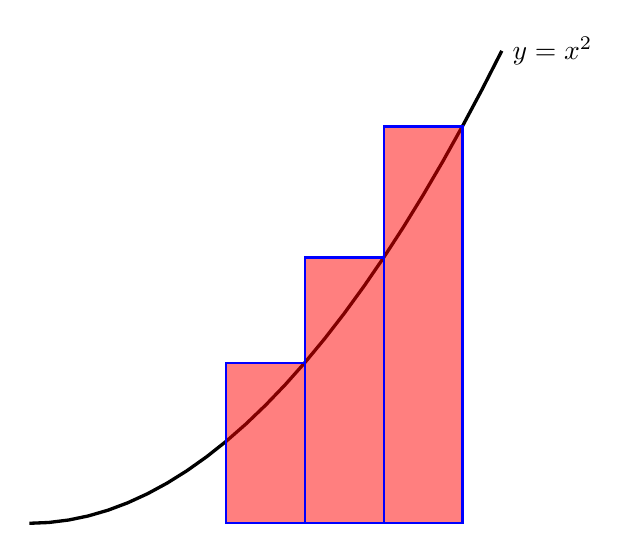
\begin{tikzpicture}
\YEaaxis{1}{7}{1}{7};
\foreach \x in {5,7,9,11}{
	\YExcoord{\x/2}{\x}}
\foreach \x in {7,9,11}{
	\MULTIPLY{\x}{\x}{\y}
	\YEycoord{\y/24}{\y}}
\draw[very thick] plot[domain=0:6] (\x,{\x*\x/6}) node[right]{$y=x^2$};
\draw[blue, thick, fill =red, fill opacity=0.5] (2.5,0) rectangle (3.5,2.04)
 (3.5,0) rectangle (4.5,3.375)
  (4.5,0) rectangle (5.5,5.04);
\end{tikzpicture}
\end{center}

\end{answer}
\begin{solution}
The general form of a Riemann sum is $\displaystyle\sum_{i=1}^n \Delta x \cdot f(x_i^*)$, where $\Delta x = \frac{b-a}{n}$ is the width of each rectangle, and $f(x_i^*)$ is the height.

There are different ways to interpret the given sum as a Riemann sum. The most obvious is given in Solution 1. You may notice that we make some convenient assumptions in this solution about values for $\Delta x$ and $a$, and we assume the sum is a right Riemann sum. Other visualizations of the sum arise from making more exotic choices. Some of these are explored in Solutions 2-4.

All cases have three rectangles, and the three rectangles will have the same areas: 98, 162, and 242 square units, respectively. This is because the terms of the given sum simplify to $98+162+242$.

\begin{description}
\item[Solution 1:]$ $
\begin{itemize}
\item Because the index runs from $1$ to $3$, there are three intervals: $n=3$.

\item Looking at our sum, it seems reasonable to interpret $\Delta x = 2$. Then, since $n=3$, we conclude $\frac{b-a}{3}=2$, hence $b-a=6$.

\item If $\Delta x = 2$, then $f(x_i^*)=\left(5+2i\right)^2$. Recall that $x_i^*$ is the $x$-coordinate we use to decide the height of the $i$th rectangle. In a right Riemann sum, $x_i^* = a+i\cdot\Delta x$. So, using $2=\Delta x$, we can let $f(x_i^*)=f(a+2i)=\left(5+2i\right)^2$. This fits with the function $f(x)=x^2$, and $a=5$.
\item Since $b-a=6$, and $a=5$, this tells us $b=11$
\end{itemize}

To sum up, we can interpret the Riemann sum as a right Riemann sum, with three intervals, of the function $f(x)=x^2$ from $x=5$ to $x=11$.


\begin{center}
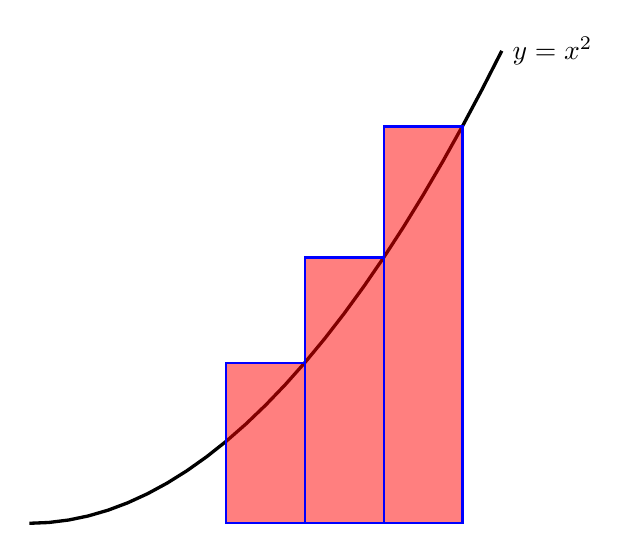
\begin{tikzpicture}
\YEaaxis{1}{7}{1}{7};
\foreach \x in {5,7,9,11}{
	\YExcoord{\x/2}{\x}}
\foreach \x in {7,9,11}{
	\MULTIPLY{\x}{\x}{\y}
	\YEycoord{\y/24}{\y}}
\draw[very thick] plot[domain=0:6] (\x,{\x*\x/6}) node[right]{$y=x^2$};
\draw[blue, thick, fill =red, fill opacity=0.5] (2.5,0) rectangle (3.5,2.04)
 (3.5,0) rectangle (4.5,3.375)
  (4.5,0) rectangle (5.5,5.04);
\end{tikzpicture}
\end{center}

\item[Solution 2: We could have chosen a different value for $\Delta x$.]
$ $
\begin{itemize}
\item The index of the sum runs from 1 to 3, so we have $n=3$.
\item We didn't have to interpret $\Delta x$ as 2--that was just the path of least resistance. We could have chosen it to be any other number--for the sake of argument, let's say $\Delta x=10$. (Positive numbers are easiest to interpret, but negatives are technically allowed as well.)

\item Then $10=\frac{b-a}{n}=\frac{b-a}{3}$, so $b-a=30$.
\item Let's use the paradigm of a right Riemann sum, and match up the terms of the sum given in the problem to the terms in the definition:
\begin{align*}
\Delta x \cdot f\left(a+i\cdot \Delta x\right)&= 2\cdot\left(5+2i\right)^2\\
10 \cdot f(a+10i)&= 2\cdot\left(5+2i\right)^2\\
f(a+10i)&=\frac{1}{5}\cdot\left(5+2i\right)^2\\
f(a+10i)&=\frac{1}{5}\cdot\left(5+\frac{1}{5}\cdot 10i\right)^2
\end{align*}
\item The easiest value of $a$ in this case is  $a=0$. Then $f(\textcolor{red}{10i}) = \frac{1}{5}\cdot\left(5+\frac{1}{5}\cdot \textcolor{red}{10i}\right)^2$, so $f(\textcolor{red}{x})= \frac{1}{5}\cdot\left(5+\frac{1}{5}\cdot \textcolor{red}{x}\right)^2$.
\item If $a=0$ and $b-a=30$, then $b=30$.
\item To sum up: $n=3$, $a=0$, $b=30$, $\Delta x = 10$, and $f(x)= \frac{1}{5}\cdot\left(5+\frac{x}{5} \right)^2$.

\begin{center}
\begin{tikzpicture}
\clip (-1.5,-1.5) rectangle (10,4);
\YEaaxis{1}{7}{1}{3};
\foreach \x in {10,20,30}{
	\YExcoord{\x/5}{\x}}
 \YEycoord{0.98}{\frac{49}{5}}
\YEycoord{1.62}{\frac{81}{5}}
\YEycoord{2.42}{\frac{121}{5}}
\draw[very thick] plot[domain=-2:35, xscale=.2, yscale=0.1] (\x,{.2*(5+\x/5)*(5+\x/5)}) ;
\draw (7,3)node[right]{$y=\frac{1}{5}\left(5+\frac{x}{5}\right)^2$};
\draw[blue, thick, fill =red, fill opacity=0.5] (0,0) rectangle (2,0.98)
 (2,0) rectangle (4,1.62)
  (4,0) rectangle (6,2.42);
\end{tikzpicture}
\end{center}
By changing $\Delta x$, we changed the \emph{widths} of the rectangles.
The rectangles in this picture are wider and shorter than the rectangles in Solution 1. Their \emph{areas} are the same: 98, 162, and 242.
\end{itemize}
\item[Solution 3: We could have chosen a different value of $a$.]
$ $
\begin{itemize}
\item Suppose $\Delta x = 2$,  and we interpret our sum as a right Riemann sum, but we didn't assume $a=5$. We could have chosen $a$ to be any number--say, $a=1$.

\item   Let's match up what we're given in the problem to what we're given as a definition:
\begin{align*}
\Delta x \cdot f\left(a+i\cdot\Delta x\right)&=2\cdot\left(5+2i\right)^2\\
2 \cdot f\left(1+2i\right)&=2\cdot\left(5+2i\right)^2\\
f\left(1+2i\right)&=\left(5+2i\right)^2\\
f\left(1+2i\right)&=\left(4+1+2i\right)^2
\end{align*}
\item Since $f(\textcolor{red}{1+2i})=\left(4+\textcolor{red}{1+2i}\right)^2$, we have $f(\textcolor{red}{x})=\left(4+\textcolor{red}{x}\right)^2$
\item Since $a=1$ and $\frac{b-a}{3}=2$, in this case $b=7$.
\item To sum up: $n=3$, $a=1$, $b=7$, $\Delta x=2$, and $f(x)=(4+x)^2$.
\begin{center}
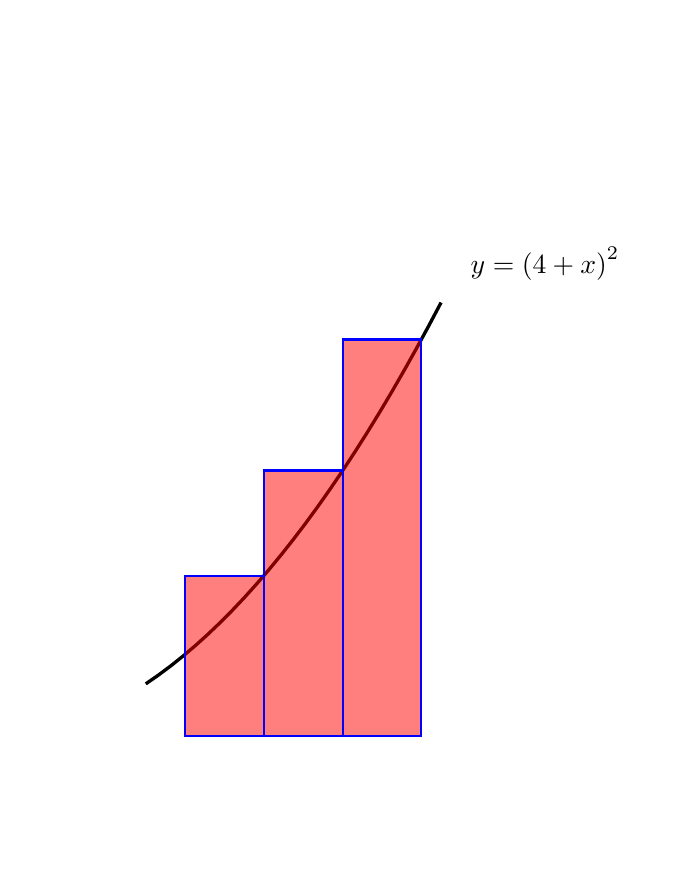
\begin{tikzpicture}
\clip (-1.5,-1.5) rectangle (6.5,9);
\YEaaxis{1}{4}{1}{6.5};
\foreach \x in {1,3,5,7}{
	\YExcoord{\x/2}{\x}}
\foreach \x in {7,9,11}{
	\MULTIPLY{\x}{\x}{\y}
	\YEycoord{\y/24}{\y}}
\draw[very thick] plot[domain=0:7.5, xscale=0.5, yscale=1/24] (\x,{(4+\x)*(4+\x)}) ;
\draw (4,6) node[right]{$y=\left(4+x\right)^2$};
\draw[blue, thick, fill =red, fill opacity=0.5] (.5,0) rectangle (1.5,2.04)
 (1.5,0) rectangle (2.5,3.375)
  (2.5,0) rectangle (3.5,5.04);
\end{tikzpicture}
\end{center}
This picture is a lot like the picture in Solution 1, but shifted to the left.
By changing $a$, we changed the \emph{left endpoint} of our region.
\end{itemize}

\item[Solution 4: We could have chosen a different kind of Riemann sum.]
$ $
\begin{itemize}
\item We didn't have to assume that we were dealing with a \emph{right} Riemann sum. Suppose $\Delta x =2$, and we have a \emph{midpoint} Riemann sum.

\item Let's match up what we're given in the problem with what we're given in the definition:
\begin{align*}
\Delta x \cdot f\left(a+\left(i-\tfrac{1}{2}\right)\Delta x\right)&=2\cdot\left(5+2i\right)^2\\
2 \cdot f\left(a+\left(i-\tfrac{1}{2}\right)2\right)&=2\cdot\left(5+2i\right)^2\\
f\left(a+\left(i-\tfrac{1}{2}\right)2\right)&=\left(5+2i\right)^2\\
f\left(a+2i-1\right)&=\left(5+2i\right)^2\\
f\left((a-1)+2i\right)&=\left(5+2i\right)^2
\end{align*}
\item It is now convenient to set $a-1=5$, hence $a=6$.
\item Then $f(\textcolor{red}{5+2i})=(\textcolor{red}{5+2i})^2$, so $f(\textcolor{red}{x})=\textcolor{red}{x}^2$
\item Since $2=\frac{b-a}{3}$ and $a=6$, we see $b=12$.
\item To sum up: $n=3$, $a=6$, $b=12$, $\Delta x = 2$, and $f(x)=x^2$.
\begin{center}
\begin{tikzpicture}
\clip (-1.5,-1.5) rectangle (9,7);
\YEaaxis{1}{7}{1}{6.5};
\foreach \x in {6,8,10,12}{
	\YExcoord{\x/2}{\x}}
\foreach \x in {7,9,11}{
	\MULTIPLY{\x}{\x}{\y}
	\YEycoord{\y/24}{\y}
	\draw[red, dashed, very thick] (\x/2,0)--(\x/2,\y/24);}
\draw[very thick] plot[domain=0:12, xscale=0.5, yscale=1/24] (\x,{\x*\x}) ;
\draw (6.5,5.5) node[right]{$y=x^2$};
\draw[blue, thick, fill =red, fill opacity=0.5] (3,0) rectangle (4,2.04)
 (4,0) rectangle (5,3.375)
  (5,0) rectangle (6,5.04);
\end{tikzpicture}
\end{center}
By choosing to interpret our sum as a midpoint Riemann sum instead of a right Riemann sum, we changed where our rectangles intersect the graph $y=f(x)$:  instead of the graph hitting the right corner of the rectangle, it hits in the middle.
\end{itemize}
\end{description}
\end{solution}


\begin{question}
Draw a picture illustrating the area given by the following Riemann sum.
\[\sum_{i=1}^5 \frac{\pi}{20}\cdot \tan\left(\frac{\pi (i-1)}{20}\right)\]
\end{question}
\begin{hint}
Let $\Delta x = \dfrac{\pi}{20}$. Then what is $b-a$?
\end{hint}
\begin{answer}
Many interpretations are possible--see the solution to Question~\ref{1.1RiemannInterp} for a more thorough discussion--but the most obvious is given below.

\begin{center}
\begin{tikzpicture}
\YEaaxis{1}{5.5}{1}{6};
\foreach \x in {2,...,5}{
	\YExcoord{\x}{\frac{\x \pi}{20}}}
	\YExcoord{1}{\frac{ \pi}{20}}
\draw[very thick] plot[domain=0:0.78, xscale=6.25, yscale=6.25] (\x,{tan(\x r)}) ;
\draw (5.25,6.225) node[right]{$y=\tan x$};
\draw[blue, thick, fill =red, fill opacity=0.5] (0,0) rectangle (1,0)
(1,0) rectangle (2,0.99)
 (2,0) rectangle (3,2.03)
  (3,0) rectangle (4,3.18)
  (4,0) rectangle (5,4.54);
\end{tikzpicture}
\end{center}

\end{answer}
\begin{solution}
Many interpretations are possible--see the solution to Question~\ref{1.1RiemannInterp} for a more thorough discussion--but the most obvious is given below. Recall the definition of a left Riemann sum:
\[\sum_{i=1}^n \Delta x \cdot f\left(a+(i-1)\Delta x\right)\]
We chose a left Riemann sum instead of right or midpoint because our given sum has $(i-1)$ in it, rather than $(i-\frac{1}{2})$ or simply $i$.
\begin{itemize}
\item Since the sum has five terms ($i$ runs from 1 to 5), there are 5 rectangles. That is, $n=5$.
\item In the definition of the Riemann sum, note that the term $\Delta x$ appears twice: once multiplied by the entire term, and once multiplied by $i-1$. So, a convenient choice for $\Delta x$ is $\frac{\pi}{20}$, because this is the constant that is both multiplied at the start of the term, and multiplied by $i-1$.
\item Since $\dfrac{\pi}{20}=\Delta x = \dfrac{b-a}{n} = \dfrac{b-a}{5}$, we see $b-a=\dfrac{5\pi}{20}=\dfrac{\pi}{4}$.
\item We match the terms in the definition with the terms in the problem:
\begin{align*}
f(a+(i-1)\Delta x) & = \tan\left(\frac{\pi (i-1)}{20}\right)\\
f\left(a+(i-1)\frac{\pi}{20}\right) & = \tan\left((i-1)\frac{\pi }{20}\right)
\end{align*}
So, we choose $a=0$ and $f(x) = \tan x$.
\item Since $a=0$ and $b-a=\frac{\pi}{4}$, we see $b=\frac{\pi}{4}$.
\end{itemize}


\begin{center}
\begin{tikzpicture}
\YEaaxis{1}{5.5}{1}{6};
\foreach \x in {2,...,5}{
	\YExcoord{\x}{\frac{\x \pi}{20}}}
	\YExcoord{1}{\frac{ \pi}{20}}
\draw[very thick] plot[domain=0:0.78, xscale=6.25, yscale=6.25] (\x,{tan(\x r)}) ;
\draw (5.25,6.225) node[right]{$y=\tan x$};
\draw[blue, thick, fill =red, fill opacity=0.5] (0,0) rectangle (1,0)
(1,0) rectangle (2,0.99)
 (2,0) rectangle (3,2.03)
  (3,0) rectangle (4,3.18)
  (4,0) rectangle (5,4.54);
\end{tikzpicture}
\end{center}
We note that the first rectangle of the five is a ``trivial" rectangle, with height (and area) 0.
\end{solution}



%%%%%%%%%%%%%%%%%%%



\begin{Mquestion}[M105 2013A]\label{1.1Riemannb}
Fill in the blanks with right, left, or midpoint;
an interval; and a value of n.

\begin{enumerate}[(a)]
\item[]
$\sum\limits_{k=0}^3 f (1.5 + k) \cdot 1$ is a
$\underline{\ \ \ \ \ \ \ \ \ \ \ \ }$
Riemann sum for $f$ on the interval
$[\,\underline{\ \ \ \ \ \ }\ ,\ \underline{\ \ \ \ \ \ }\,]$ with
$n =\underline{\ \ \ \ \ }$.
\end{enumerate}
\end{Mquestion}

\begin{hint}
Notice that the index starts at $k=0$, instead of $k=1$.
Write out the given sum explicitly without using summation notation, and sketch where the rectangles would fall on a graph of $y=f(x)$.
%Also write out the first few terms in the sums in the three bullets of
%Definition \eref{CLP101}{def:INTthreeRiemannSums} in the
%\href{http://www.math.ubc.ca/%7Efeldman/m101/clp/clp_notes_101.pdf}{CLP-II text}.
%CLP-2 text.
Then try to identify $b-a$, and $n$,
followed by ``right'', ``left'', or ``midpoint'', and finally $a$.
\end{hint}

\begin{answer}
Three answers are possible.
It is a
midpoint Riemann sum for $f$ on the interval $[1,5]$ with $n =4$.
It is also a left Riemann sum for $f$ on the interval $[1.5,5.5]$ with $n =4$.
It is also a right Riemann sum for $f$ on the interval $[0.5,4.5]$ with $n =4$.
\end{answer}

\begin{solution}
Since there are four terms in the sum, $n=4$. (Note the sum starts at $k=0$, instead of $k=1$.) Since the function is multiplied by 1, $1=\Delta x=\dfrac{b-a}{n}=\dfrac{b-a}{4}$, hence $b-a=4$.

We can choose to view the given sum as a left, right, or midpoint Riemann sum. The choice we make determines the interval. Note that the heights of the rectangles are determined when $x = 1.5,\, 2.5,\, 3.5,$ and $4.5$.
\begin{center}
\begin{tikzpicture}
\YEaaxis{.5}{5.5}{.5}{5}
\foreach \k in {1,...,4}{
	\YEycoord{\k}{f(\k.5)}
	\ADD{\k}{1}{\l}
	\draw[thick, fill=blue, fill opacity=0.5] (\k,0) rectangle (\l,\k);}
\end{tikzpicture}
\end{center}
\begin{description}
\item[Option 1: right Riemann sum]
If our sum is a right Riemann sum, then we take the heights of the rectangles from the right endpoint of each interval.
\begin{center}
\begin{tikzpicture}
\YEaaxis{.5}{5.5}{.5}{5}
\foreach \k in {1,...,4}{
	\YEycoord{\k}{f(\k.5)}
	\ADD{\k}{1}{\l}
	\draw[thick, fill=blue, fill opacity=0.5] (\k,0) rectangle (\l,\k);
	\draw(\l,\k)node[vertex]{};
	\YExcoord{\l}{\k.5}}
\draw[thick] (2,1)--(5,4);
\end{tikzpicture}
\end{center}

Then $a=0.5$ and $b=4.5$. Therefore: $\sum\limits_{k=0}^3 f (1.5 + k) \cdot 1$ is a right Riemann sum on the interval $[0.5,4.5]$ with $n=4$.
\item[Option 2: left Riemann sum]
If our sum is a left Riemann sum, then we take the heights of the rectangles from the left endpoint of each interval.

\begin{center}
\begin{tikzpicture}
\YEaaxis{.5}{5.5}{.5}{5}
\foreach \k in {1,...,4}{
	\YEycoord{\k}{f(\k.5)}
	\ADD{\k}{1}{\l}
	\draw[thick, fill=blue, fill opacity=0.5] (\k,0) rectangle (\l,\k);
	\draw(\k,\k)node[vertex]{};
	\YExcoord{\k}{\k.5}}
	\draw[thick] (1,1)--(4,4);
\end{tikzpicture}
\end{center}

Then $a=1.5$ and $b=5.5$. Therefore: $\sum\limits_{k=0}^3 f (1.5 + k) \cdot 1$ is a left Riemann sum on the interval $[1.5,5.5]$ with $n=4$.
\item[Option 3: midpoint Riemann sum]
If our sum is a midpoint Riemann sum, then we take the heights of the rectangles from the midpoint of each interval.

\begin{center}
\begin{tikzpicture}
\YEaaxis{.5}{5.5}{.5}{5}
\foreach \k in {1,...,4}{
	\YEycoord{\k}{f(\k.5)}
	\ADD{\k}{1}{\l}
	\ADD{\k}{.5}{\m}
	\draw[thick, fill=blue, fill opacity=0.5] (\k,0) rectangle (\l,\k);
	\draw(\m,\k)node[vertex]{};
	\YExcoord{\m}{\k.5}}
\draw[thick] (1.5,1)--(4.5,4);
\end{tikzpicture}
\end{center}

Then $a=1$ and $b=5$. Therefore: $\sum\limits_{k=0}^3 f (1.5 + k) \cdot 1$ is a midpoint Riemann sum on the interval $[1,5]$ with $n=4$.

\end{description}
\end{solution}
%%%%%%%%%%%%%%%%%%%

\begin{question}
Evaluate the following integral by interpreting it as a signed area, and using geometry:
\[\int_0^5 x \,\dee{x}\]
\end{question}
\begin{hint}
The area is a triangle.
\end{hint}
\begin{answer}
$\dfrac{25}{2}$
\end{answer}
\begin{solution}
The area in question is a triangle with base 5 and height 5, so its area is $\dfrac{25}{2}$.
\begin{center}
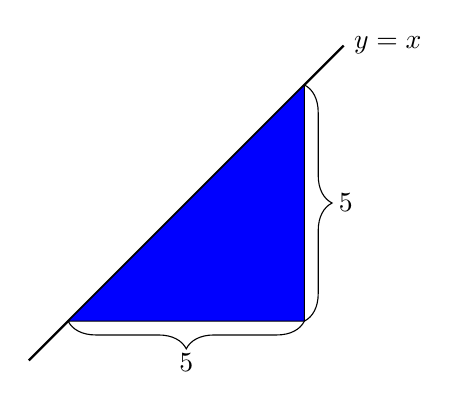
\begin{tikzpicture}
\YEaaxis{1}{4}{1}{4}
\draw[thick] (-.5,-.5)--(3.5,3.5) node[right]{$y=x$};
\draw[fill=blue] (0,0)--(3,3)--(3,0)--cycle;
\YEycoord{3}{5}
\draw[decorate, decoration={brace, amplitude=10pt}] (3,0)--(0,0) node[midway, yshift=-15pt]{$5$};
\draw[decorate, decoration={brace, amplitude=10pt}] (3,3)--(3,0) node[midway, xshift=15pt]{$5$};
\end{tikzpicture}
\end{center}
\end{solution}



\begin{Mquestion}
Evaluate the following integral by interpreting it as a signed area, and using geometry:
\[\int_{-2}^5 x \,\dee{x}\]
\end{Mquestion}
\begin{hint} There is one triangle of positive area, and one of negative area.
\end{hint}
\begin{answer}
$\dfrac{21}{2}$
\end{answer}
\begin{solution}

There is a positive and a negative portion of this area. The positive area is a triangle with base 5 and height 5, so area $\dfrac{25}{2}$ square units. The negative area is a triangle with base $2$ and height $2$, so negative area $\dfrac{4}{2}=2$ square units. So, the net area is $\dfrac{25}{2}-\dfrac{4}{2}=\dfrac{21}{2}$ square units.
\begin{center}
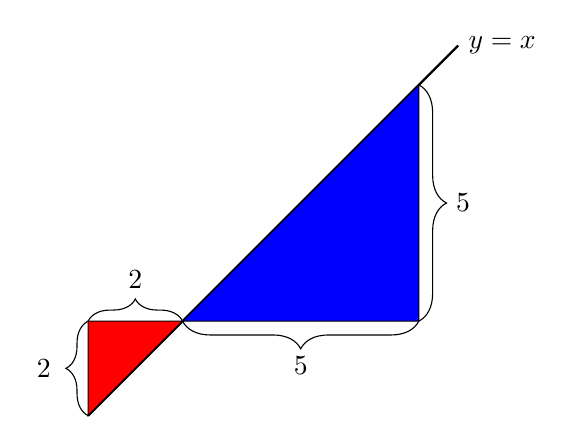
\begin{tikzpicture}
\YEaaxis{2}{4}{2}{4}
\draw[thick] (-1.2,-1.2)--(3.5,3.5) node[right]{$y=x$};
\draw[fill=blue] (0,0)--(3,3)--(3,0)--cycle;
\draw[fill=red] (0,0)--(-1.2,-1.2)--(-1.2,0)--cycle;
\YEycoord{3}{5}
\draw[decorate, decoration={brace, amplitude=10pt}] (3,0)--(0,0) node[midway, yshift=-16pt]{$5$};
\draw[decorate, decoration={brace, amplitude=10pt}] (3,3)--(3,0) node[midway, xshift=16pt]{$5$};
\draw[decorate, decoration={brace, amplitude=8pt}] (-1.2,0)--(0,0) node[midway, yshift=15pt]{$2$};
\draw[decorate, decoration={brace, amplitude=8pt}] (-1.2,-1.2)--(-1.2,0) node[midway, xshift=-16pt]{$2$};
\end{tikzpicture}
\end{center}
\end{solution}




%%%%%%%%%%%%%%%%%%
\subsection*{\Procedural}
%%%%%%%%%%%%%%%%%%

\begin{question}[M105 2014A]
Use sigma notation to write the midpoint Riemann sum for $f(x)=x^8$ on $[5,15]$
with $n=50$. Do not evaluate the Riemann sum.
\end{question}

\begin{hint}
Review Definition  \eref{CLP101}{def:INTthreeRiemannSums} in the
%\href{http://www.math.ubc.ca/%7Efeldman/m101/clp/clp_notes_101.pdf}{CLP 101 notes}
CLP-2 text.
\end{hint}

\begin{answer}
$\sum\limits_{i=1}^{50} \Big(5+\big(i-\nicefrac{1}{2}\big)\frac{1}{5}\Big)^8
\ \frac{1}{5}$
\end{answer}

\begin{solution}
In general, the midpoint Riemann sum is given by
\begin{align*}
\sum_{i=1}^n f\Big(a+\big(i-\nicefrac{1}{2}\big)\De x\Big)\ \De x \, ,
\qquad \mbox{where } \De x = \frac{b-a}{n}.
\end{align*}
In this problem we are told that $f(x)=x^8$, $a=5$, $b=15$ and $n=50$,
so that $\De x = \frac{b-a}{n} = \frac{1}{5}$ and the desired Riemann sum is:
\begin{align*}
\sum_{i=1}^{50} \Big(5+\big(i-\nicefrac{1}{2}\big)\frac{1}{5}\Big)^8
\ \frac{1}{5}
\end{align*}
\end{solution}
%%%%%%%%%%%%%%%%%%%




\begin{question}[2016Q1]
Estimate $\displaystyle\int_{-1}^5 x^3\,\,\dee{x}$ using three approximating rectangles
and left hand end points.
\end{question}

%\begin{hint}
%\end{hint}

\begin{answer}
$54$
\end{answer}

\begin{solution}
The given integral has interval of integration going from $a=-1$ to $b=5$.
So when we use three approximating rectangles, all of the same width, the common width
is $\Delta x=\frac{b-a}{n} = 2$. The first rectangle has left  endpoint $x_0=a=-1$,
the second has left hand endpoint $x_1=a+\Delta x=1$, and the third has left hand end point
$x_2=a+2\Delta x=3$. So
\begin{align*}
\int_{-1}^5 x^3\,\,\dee{x}
\approx \big[f(x_0)+f(x_1)+f(x_2)\big]\Delta x
=\big[(-1)^3+1^3+3^3\big]\times2
=54
\end{align*}
\end{solution}

%%%%%%%%%%%%%%%%%



\begin{Mquestion}[2016Q1]
Let $f$ be a function on the whole real line.  Express
$\displaystyle\int_{-1}^{7}f(x)\,\,\dee{x}$ as a limit of Riemann sums, using the
right endpoints.
\end{Mquestion}

\begin{hint}
You'll want the limit as $n$ goes to infinity of a sum with $n$ terms. If you're having a hard time coming up with the sum in terms of $n$, try writing a sum with a finite number of terms of your choosing. Then, think about how that sum would change if it had $n$ terms.
\end{hint}

\begin{answer}
$\displaystyle\int_{-1}^{7}f(x)\,\,\dee{x}=\displaystyle\lim_{n\to\infty}\displaystyle\sum_{i=1}^{n} f\left(-1+\frac{8i}{n}\right)\frac{8}{n}$
\end{answer}

\begin{solution}
In the given integral, the domain of integration runs from $a=-1$ to $b=7$.
So, we have $\Delta x = \frac{(b-a)}{n}= \frac{(7-(-1))}{n} = \frac{8}{n}$. The left-hand end of the first
subinterval is at $x_0=a=-1$. So, the right-hand end of the $i^{\rm th}$ interval
is at $x_i^* = -1+\frac{8i}{n}$. So:
\begin{align*}
\int_{-1}^{7}f(x)\,\,\dee{x}
=\lim_{n\to\infty}\sum_{i=1}^{n} f\left(-1+\frac{8i}{n}\right)\frac{8}{n}
\end{align*}

\end{solution}

%%%%%%%%%%%%%%%
\begin{question}[2016Q1]
The value of the following limit is equal to the area below a graph of $y=f(x)$, integrated over the interval $[0,b]$:
\begin{align*}
   \lim_{n \to \infty} \sum_{i=1}^{n} \frac{4}{n}
          \left[ \sin \left( 2 + \frac{4i}{n}\right)\right]^2
\end{align*}
Find $f(x)$ and $b$.
\end{question}

\begin{hint}
The main step is to express the given sum as the right Riemann sum,
\[\sum_{i=1}^{n} f(a+i\De x)\Delta  x.\]
Don't be afraid to guess $\De x$ and $f(x$)
(review Definition  \eref{CLP101}{def:INTthreeRiemannSums} in the
%\href{http://www.math.ubc.ca/%7Efeldman/m101/clp/clp_notes_101.pdf}{CLP 101 notes}
CLP-2 text).
Then write out explicitly $ \sum\limits_{i=1}^{n} f(a+i\De x)\Delta  x$
with your guess substituted in, and compare the result with the given sum.  Adjust your guess if they don't match.
\end{hint}

\begin{answer}
$f(x) = \sin^2 (2 + x)$ and $b=4$
\end{answer}

\begin{solution}
We identify the given sum as the right Riemann sum
$\sum\limits_{i=1}^{n} f(a+i\De x)\Delta  x$,
with $a=0$ (that's specified in the statement of the question). Since $\frac{4}{n}$ is multiplied in every term, and is also multiplied by $i$, we let
 $\Delta x = \frac{4}{n}$. Then $x_i^* = a+i\De x=\frac{4i}{n}$
and $f(x) = \sin^2 (2 + x)$. So, $b=a+n\De x=0+n\cdot\frac{4}{n}=4$.
\end{solution}
%%%%%%%%%%%%%%%%%%%

\begin{Mquestion}[M105 2102A]
For a certain function $f(x)$, the following equation holds:
\begin{equation*}
\lim_{n\rightarrow\infty}\sum\limits_{k=1}^n
\frac{k}{n^2}\sqrt{1-\frac{k^2}{n^2}}
=\int_0^1 f(x)\ \,\dee{x}
\end{equation*}
Find $f(x)$.
\end{Mquestion}

\begin{hint}
The main step is to express the given sum as the right Riemann sum
$\sum\limits_{k=1}^{n} f(a+k\De x)\Delta  x$.
Don't be afraid to guess $\De x$ and $f(x$)
(review Definition  \eref{CLP101}{def:INTthreeRiemannSums} in the
%\href{http://www.math.ubc.ca/%7Efeldman/m101/clp/clp_notes_101.pdf}{CLP 101 notes}
CLP-2 text).
Then write out explicitly $ \sum\limits_{k=1}^{n} f(a+k\De x)\Delta  x$
with your guess substituted in, and compare the result with the given sum.  Adjust your guess if they don't match.
\end{hint}

\begin{answer}
$f(x)=x\sqrt{1-x^2}$
\end{answer}

\begin{solution}
The given sum is of the form
\begin{align*}
\lim_{n\rightarrow\infty}\sum_{k=1}^n
             \frac{k}{n^2}\sqrt{1-\frac{k^2}{n^2}}
=\lim_{n\rightarrow\infty}\sum_{k=1}^n
            \left(\frac{1}{n}\right) \frac{k}{n}\sqrt{1-\left(\frac{k}{n}\right)^2}
=\lim_{n\rightarrow\infty}\sum_{k=1}^n \De x f(x_k^*)
\end{align*}
with $\De x=\frac{1}{n}$, $a=0$, $x_k^*=\frac{k}{n}=a+k\De x$
and $f(x)=x\sqrt{1-x^2}$.
Since $x_0^*=0$ and $x_n^*=1$, the right hand side is the definition
(using the right Riemann sum) of
$
\int_0^1 f(x)\,\,\dee{x}
$.

\end{solution}
%%%%%%%%%%%%%%%%%%%


\begin{question}[2016Q1]
Express $\displaystyle\lim_{n\to\infty}\displaystyle\sum_{i=1}^{n}
                       \frac{3}{n} e^{-i/n} \cos\left(\frac{3i}{n}\right)$
as a definite integral.
\end{question}

\begin{hint}
The main step is to express the given sum in the form $ \sum_{i=1}^{n} f(x_i^*)\Delta  x$.
Don't be afraid to guess $\De x$, $x_i^*$ (for either a left or a right or a  midpoint sum ---
review Definition  \eref{CLP101}{def:INTthreeRiemannSums} in the
%\href{http://www.math.ubc.ca/%7Efeldman/m101/clp/clp_notes_101.pdf}{CLP 101 notes}
CLP-2 text)
and $f(x$). Then write out explicitly $ \sum_{i=1}^{n} f(x_i^*)\Delta  x$ with your guess
substituted in, and compare the result with the given sum.  Adjust your guess if they don't match.
\end{hint}

\begin{answer}
$\int_0^3 e^{-x/3}\cos(x)\,\,\dee{x}$
\end{answer}

\begin{solution}
As $i$ ranges from $1$ to $n$, $3i/n$ range from $3/n$ to $3$ with jumps of
$\De x=3/n$, so this is
\begin{align*}
\lim_{n\to\infty}\displaystyle\sum_{i=1}^{n}
                       \frac{3}{n} e^{-i/n} \cos(3i/n)
=\lim_{n\to\infty} \sum_{i=1}^{n} f(x_i^*)\Delta  x
=\int_a^b f(x)\,\,\dee{x}
\end{align*}
where $x_i^* = 3i/n$, $f(x) = e^{-x/3}\cos(x)$, $a=x_0=0$ and $b=x_n=3$. Thus
\begin{align*}
\lim_{n\to\infty}\displaystyle\sum_{i=1}^{n}
                       \frac{3}{n} e^{-i/n} \cos(3i/n)
=\int_0^3 e^{-x/3}\cos(x)\,\,\dee{x}
\end{align*}

\end{solution}
%%%%%%%%%%%%%%%%%%%

\begin{question}[2012A, 2014D]
Let $\displaystyle R_n= \sum_{i=1}^{n}
                       \frac{i e^{i/n}}{n^2}$.
Express $\displaystyle\lim_{n\to\infty}R_n$
as a definite integral. \emph{Do not evaluate this integral.}
\end{question}

\begin{hint}
The main step is to express the given sum in the form
$\sum\limits_{i=1}^{n} f(x_i^*)\Delta  x$.
Don't be afraid to guess $\De x$, $x_i^*$ (probably, based on the symbol $R_n$,
assuming we have a right Riemann sum ---
review Definition  \eref{CLP101}{def:INTthreeRiemannSums} in the CLP-2 text)
and $f(x$). Then write out explicitly $ \sum\limits_{i=1}^{n} f(x_i^*)\Delta  x$ with
your guess substituted in, and compare the result with the given sum.
Adjust your guess if they don't match.
\end{hint}

\begin{answer}
$\displaystyle\int_0^1 x e^{x}\,\,\dee{x}$
\end{answer}

\begin{solution}
As $i$ ranges from $1$ to $n$, the exponent $\frac{i}{n}$ ranges from $\frac{1}{n}$ to $1$ with
jumps of $\De x=\frac{1}{n}$. So let's try $x_i^* =\frac{ i}{n}$, $\Delta x=\frac{1}{n}$. Then:
\begin{align*}
R_n= \sum_{i=1}^{n} \frac{i e^{i/n}}{n^2}
= \sum_{i=1}^{n} \frac{i}{n} e^{i/n} \frac{1}{n}
= \sum_{i=1}^{n} x_i^* e^{x_i^*} \Delta x
= \sum_{i=1}^{n} f(x_i^*) \Delta x
\end{align*}
with $f(x)= x e^x$, and the limit
\begin{align*}
\lim_{n\to\infty} R_n
=\lim_{n\to\infty} \sum_{i=1}^{n} f(x_i^*)\Delta  x
=\int_a^b f(x)\,\,\dee{x}
\end{align*}
Since we chose $x_i^* = \frac{i}{n} = 0+i\De x$, we let $a=0$. Then $\frac{1}{n}=\De x = \frac{b-a}{n}=\frac{b}{n}$ tells us $b=1$. Thus,
\begin{align*}
\lim_{n\to\infty}R_n
=\int_0^1 xe^{x}\,\,\dee{x}\,.
\end{align*}

\end{solution}
%%%%%%%%%%%%%%%%%%%


\begin{Mquestion}[2016A]
Express
$\displaystyle\lim_{n\rightarrow\infty} \bigg( \sum_{i=1}^n e^{-1-2i/n}\cdot \frac{2}{n} \bigg)$
as an integral in three different ways.
\end{Mquestion}

\begin{hint}
Try several different choices of $\De x$ and $x_i^*$.
\end{hint}

\begin{answer}
Possible answers include:\\[5pt] $\displaystyle\int\limits_0^2 e^{-1-x}\ \,\dee{x}$,\quad
                                $\displaystyle\int\limits_1^3 e^{-x}\ \,\dee{x}$, \quad
                                $2\displaystyle\int_{1/2}^{3/2} e^{-2x}\ \,\dee{x}$, \quad
and \quad
                                $2\displaystyle\int\limits_0^1 e^{-1-2x}\ \,\dee{x}$.
\end{answer}

\begin{solution}
\begin{description}
\item[Choice \#1:]
If we set $\De x = \frac{2}{n}$ and $x_i^*= \frac{2i}{n}$, i.e. $x_i^* = a + i\De x$ with $a=0$,
then
\begin{align*}
\lim_{n\rightarrow\infty} \bigg( \sum_{i=1}^n e^{-1-2i/n}\cdot \frac{2}{n} \bigg)
&=\lim_{n\rightarrow\infty} \bigg( \sum_{i=1}^n e^{-1-x_i^*}\De x \bigg) \hidewidth \\
&=\lim_{n\rightarrow\infty} \bigg( \sum_{i=1}^n f(x_i^*)\De x \bigg) &&\text{with $f(x) = e^{-1-x}$} \\
&=\int_a^b f(x)\,\,\dee{x}&&\text{with $a=x_0=0$ and $b=x_n=2$} \\
&=\int_0^2 e^{-1-x}\ \,\dee{x}
\end{align*}


\item[Choice \#2:]
If we set $\De x = \frac{2}{n}$ and $x_i^*= 1+\frac{2i}{n}$, i.e. $x_i^* = a + i\De x$
with $a=1$,
then
\begin{align*}
\lim_{n\rightarrow\infty} \bigg( \sum_{i=1}^n e^{-1-2i/n}\cdot \frac{2}{n} \bigg)
&=\lim_{n\rightarrow\infty} \bigg( \sum_{i=1}^n e^{-x_i^*}\De x \bigg) \hidewidth \\
&=\lim_{n\rightarrow\infty} \bigg( \sum_{i=1}^n f(x_i^*)\De x \bigg) &&\text{with $f(x) = e^{-x}$} \\
&=\int_a^b f(x)\,\,\dee{x}&&\text{with $a=x_0=1$ and $b=x_n=3$} \\
&=\int_1^3 e^{-x}\ \,\dee{x}
\end{align*}

\item[Choice \#3:]
If we set $\De x = \frac{1}{n}$ and $x_i^*= \frac{i}{n}$, i.e. $x_i^* = a + i\De x$ with $a=0$,
then
\begin{align*}
\lim_{n\rightarrow\infty} \bigg( \sum_{i=1}^n e^{-1-2i/n}\cdot \frac{2}{n} \bigg)
&=\lim_{n\rightarrow\infty} \bigg( \sum_{i=1}^n e^{-1-2x_i^*}\ 2\De x \bigg) \hidewidth \\
&=\lim_{n\rightarrow\infty} \bigg( \sum_{i=1}^n f(x_i^*)\De x \bigg)
                       &&\text{with $f(x) = 2e^{-1-2x}$} \\
&=\int_a^b f(x)\,\,\dee{x}&&\text{with $a=x_0=0$ and $b=x_n=1$} \\
&=2\int_0^1 e^{-1-2x}\ \,\dee{x}
\end{align*}

\item[Choice \#4:]
If we set $\De x = \frac{1}{n}$ and $x_i^*= \frac{1}{2}+\frac{i}{n}$, i.e. $x_i = a + i\De x$
with $a=\frac{1}{2}$,
then
\begin{align*}
\lim_{n\rightarrow\infty} \bigg( \sum_{i=1}^n e^{-1-2i/n}\cdot \frac{2}{n} \bigg)
&=\lim_{n\rightarrow\infty} \bigg( \sum_{i=1}^n e^{-2x_i}\ 2\De x \bigg) \hidewidth \\
&=\lim_{n\rightarrow\infty} \bigg( \sum_{i=1}^n f(x_i^*)\De x \bigg)
                       &&\text{with $f(x) = 2e^{-2x}$} \\
&=\int_a^b f(x)\,\,\dee{x}&&\text{with $a=x_0=\frac{1}{2}$ and $b=x_n=\frac{3}{2}$} \\
&=2\int_{1/2}^{3/2} e^{-2x}\ \,\dee{x}
\end{align*}

\end{description}

\end{solution}
%%%%%%%%%%%%%%%%%%%


\Instructions{Questions~\ref{1.1geoma} and \ref{1.1geomb} use the formula for a geometric sum, Equation~\eref{CLP101}{eq:INTgeomsum} in the CLP-2 text.}

\begin{Mquestion}\label{1.1geoma}
Evaluate the sum $1+r^3+r^6+r^9+\cdots+r^{3n}$.
\end{Mquestion}
\begin{hint}
Let $x=r^3$, and re--write the sum in terms of $x$.
\end{hint}
\begin{answer}
$\dfrac{r^{3n+3}-1}{r-1}$
\end{answer}
\begin{solution}
This is similar to the familiar form of a geometric sum, but the powers go up by threes. So, we make a subsitution. If $x=r^3$, then:
\[
1+r^3+r^6+r^9+\cdots+r^{3n}=1+x+x^2+x^3+\cdots+x^n\]
Now, using Equation~\eref{CLP101}{eq:INTgeomsum} in the CLP-2 text,
\[
1+x+x^2+x^3+\cdots+x^n = \frac{x^{n+1}-1}{x-1}\]
Substituting back in $x=r^3$, we find our sum is equal to $\dfrac{(r^3)^{n+1}-1}{r^3-1}$, or
$\dfrac{r^{3n+3}-1}{r^3-1}$.
\end{solution}

\begin{Mquestion}\label{1.1geomb}
Evaluate the sum $r^5+r^6+r^7+\cdots+r^{100}$.
\end{Mquestion}
\begin{hint}
Note the sum does not start at $r^0=1$.
\end{hint}
\begin{answer}
$r^5\left(\dfrac{r^{96}-1}{r-1}\right)$
\end{answer}
\begin{solution}
The sum does not start at $1$, so we need to do some algebra. We can either factor out the first term, or subtract off the initial terms that are missing.
\begin{description}
\item[Solution 1:]
If we factor out $r^5$, then what's left fits the form of
Equation~\eref{CLP101}{eq:INTgeomsum} in the CLP-2 text:
\[r^5+r^6+r^7+\cdots+r^{100}=r^5\left[1+r+r^2+\cdots + r^{95}\right]= r^5\left(\frac{r^{96}-1}{r-1}\right)\ .\]
\item[Solution 2:] We know how to evaluate sums of this form if they start at 1, so we re-write our sum as follows:
\begin{align*}
r^5+r^6+r^7+\cdots+r^{100}&=\left(1+r+r^2+r^3+r^4+r^5+\cdots+r^{100}\right) -
\left(1+r+r^2+r^3+r^4\right) \\
&=\frac{r^{101}-1}{r-1} - \frac{r^5-1}{r-1}\\
&=\frac{r^{101}-1-r^5+1}{r-1}=\frac{r^{101}-r^5}{r-1}=r^5\left(\frac{r^{96}-1}{r-1}\right)\ .
\end{align*}
\end{description}
\end{solution}


\Instructions{Remember that a definite integral is a signed area between a curve and the $x$-axis. We'll spend a lot of time learning strategies for evaluating definite integrals, but we already know lots of ways to find area of geometric shapes. In Questions~\ref{1.1defintgeoma} through \ref{1.1defintgeomb}, use your knowledge of geometry to find the signed areas described by the integrals given.}


\begin{question}[M105 2013A]\label{prob:s1.1_2}\label{1.1defintgeoma}
Evaluate ${\displaystyle\int_{-1}^2 |2x|\ \,\dee{x}}$.
\end{question}

\begin{hint}
Draw a picture. See Example \eref{CLP101}{eg:INTtriangleB} in the
%\href{http://www.math.ubc.ca/%7Efeldman/m101/clp/clp_notes_101.pdf}{CLP 101 notes}.
CLP-2 text.
\end{hint}

\begin{answer}
$5$
\end{answer}

\begin{solution}
Recall that
\begin{align*}
|x|=\begin{cases} -x &\text{if $x\le 0$}\\
                   x &\text{if $x\ge 0$}
    \end{cases}
\end{align*}
so that
\begin{align*}
|2x|=\begin{cases} -2x &\text{if $x\le 0$}\\
                    2x &\text{if $x\ge 0$}
    \end{cases}
\end{align*}
To picture the geometric figure whose area the integral represents
observe that
\begin{itemize}\itemsep1pt \parskip0pt \parsep0pt %\itemindent-15pt
\item
at the left hand end of the domain of integration $x=-1$ and
the integrand $|2x|=|-2|=2$ and
\item
as $x$ increases from $-1$ towards $0$, the integrand $|2x|=-2x$ decreases
linearly, until
\item
when $x$ hits $0$ the integrand hits  $|2x|=|0|=0$ and then
\item
as $x$ increases from $0$, the integrand $|2x|=2x$ increases
linearly, until
\item
when $x$ hits $+2$, the right hand end of the domain of integration, the
integrand hits
$|2x|=|4|=4$.
\end{itemize}
So the integral $\int_{-1}^2 |2x|\ \,\dee{x}$  is the area of
the union of the two shaded triangles (one of base $1$ and of height $2$
and the other of base $2$ and height $4$) in the figure on
the right below and
\begin{align*}
\int_{-1}^2 |2x|\ \,\dee{x}
= \frac{1}{2}\times 1\times 2 + \frac{1}{2}\times 2\times 4
= 5\qquad\qquad
\raisebox{-0.5\height}{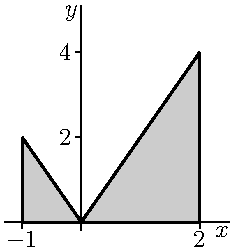
\includegraphics{OEM105_13A_1e}}
\end{align*}


\end{solution}
%%%%%%%%%%%%%%%%%%%

\begin{Mquestion}
Evaluate the following integral by interpreting it as a signed area, and using geometry:
\[\int_{-3}^5 |t-1| \,\dee{t}\]
\end{Mquestion}
\begin{hint}
Draw a picture. Remember $|x| = \left\{\begin{array}{rc}x&x\ge 0\\-x&x<0\end{array}\right.$\ .
\end{hint}
\begin{answer}
16
\end{answer}
\begin{solution}
The area we want is two triangles, both above the $x$-axis. Each triangle has base $4$ and height $4$, so the total area is $2\cdot\left(\dfrac{4\cdot 4}{2}\right)=16$.
\begin{center}
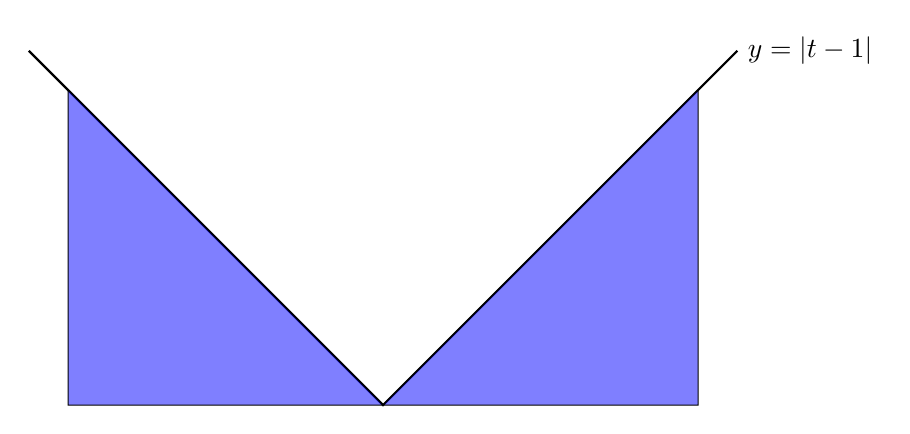
\begin{tikzpicture}
\YEaaxis{5}{6}{1}{5}
\draw[thick] (-3.5,4.5)--(1,0)--(5.5,4.5) node[right]{$y=|t-1|$};
\draw[fill=blue, fill opacity=0.5] (-3,0)--(-3,4)--(1,0)--(5,4)--(5,0)--cycle;
\YExcoord{5}{5}
\YExcoord{1}{1}
\YExcoord{-3}{-3}
\YEycoord{4}{4}
\end{tikzpicture}
\end{center}
If you had a hard time sketching the function, recall that the absolute value of a number leaves it unchanged if it is positive or zero, and flips the sign if it is negative. So, when $t-1 \ge 0$ (that is, when $t \ge 1$), our function is simply $f(t)=|t-1|=t-1$. On the other hand, when $t=1$ is negative (that is, when $t<1$), the absolute value changes the sign, so $f(t) = |t-1|=-(t-1)=-t+1$.
\end{solution}

\begin{question}\label{1.1trapezoidarea}
Evaluate the following integral by interpreting it as a signed area, and using geometry:
\[\int_a^b x \,\dee{x}\]
where $0 \leq a \leq b$.
\end{question}
\begin{hint}
Draw a picture: the area we want is a trapezoid. If you don't remember a formula for the area of a trapezoid, think of it as the difference of two triangles.
\end{hint}
\begin{answer}
$\dfrac{b^2-a^2}{2}$
\end{answer}
\begin{solution}
The area we want is a trapezoid with base $(b-a)$ and heights $a$ and $b$, so its area is $\dfrac{(b-a)(b+a)}{2}=\dfrac{b^2-a^2}{2}$.
\begin{center}
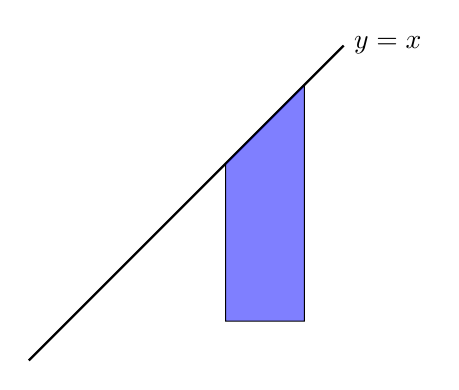
\begin{tikzpicture}
\YEaaxis{1}{4}{1}{4}
\draw[thick] (-.5,-.5)--(3.5,3.5) node[right]{$y=x$};
\draw[fill=blue, fill opacity=0.5] (2,0)--(2,2)--(3,3)--(3,0)--cycle;
\YExcoord{3}{b}
\YEycoord{3}{b}
\YExcoord{2}{a}
\YEycoord{2}{a}
\end{tikzpicture}
\end{center}
Instead of using a formula for the area of a trapezoid, you can find the blue area as the area of a triangle with base and height $b$, minus the area of a triangle with base and height $a$.
\end{solution}

\begin{question}
Evaluate the following integral by interpreting it as a signed area, and using geometry:
\[\int_a^b x\, \dee{x}\]
where $a \leq b \leq 0$.
\end{question}
\begin{hint}
You can draw a very similar picture to Question~\ref{1.1trapezoidarea}, but remember the areas are negative.
\end{hint}
\begin{answer}
$\dfrac{b^2-a^2}{2}$
\end{answer}
\begin{solution}
The area is negative. The shape is a trapezoid with base length $(b - a)$ and heights
        $0-a=-a$ and $0-b=-b$ (note: those are nonnegative numbers), so its area is $\dfrac{(b-a)(-b-a)}{2}=\dfrac{-b^2+a^2}{2}$. Since the shape is below the $x$-axis, we change its sign. Thus, the integral evaluates to\ $\dfrac{b^2-a^2}{2}$.
\begin{center}
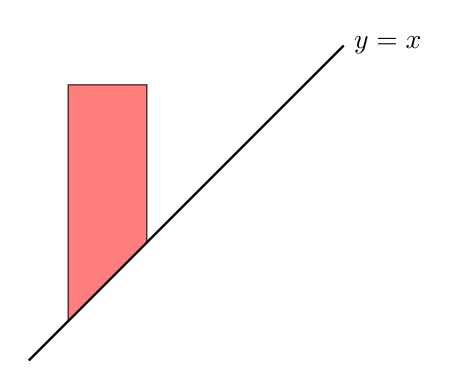
\begin{tikzpicture}
\YEaaxis{4}{1}{4}{1}
\draw[thick] (-3.5,-3.5)--(.5,.5) node[right]{$y=x$};
\draw[fill=red, fill opacity=0.5] (-2,0)--(-2,-2)--(-3,-3)--(-3,0)--cycle;
\YEnxcoord{-3}{a}
\YEnycoord{-3}{a}
\YEnxcoord{-2}{b}
\YEnycoord{-2}{b}
\end{tikzpicture}
\end{center}

The signs can be a little hard to keep track of. The base of our trapezoid is $|a-b|$;  since $b>a$, this is $b-a$. The heights of the trapezoid are  $|a|$ and $|b|$; since these are both negative, $|a|=-a$ and $|b|=-b$.

We note that this is the same result as in Question~\ref{1.1trapezoidarea}.
\end{solution}


\begin{Mquestion}
Evaluate the following integral by interpreting it as a signed area, and using geometry:
\[\int_0^4 \sqrt{16-x^2} \ \dee{x}\]
\end{Mquestion}
\begin{hint}
If $y=\sqrt{16-x^2}$, then $y$ is nonnegative, and $y^2+x^2=16$.
\end{hint}
\begin{answer}
$4\pi$
\end{answer}
\begin{solution}
If $y=\sqrt{16-x^2}$, then $y$ is nonnegative, and $y^2+x^2=16$. So, the graph $y=\sqrt{16-x^2}$ is the upper half of a circle of radius 4. Since $x$ only runs from 0 to 4, we have a quarter of a circle of radius 4. Then the area under the curve is $\dfrac{1}{4}\left[\pi\cdot 4^2\right]=4\pi$.
\begin{center}
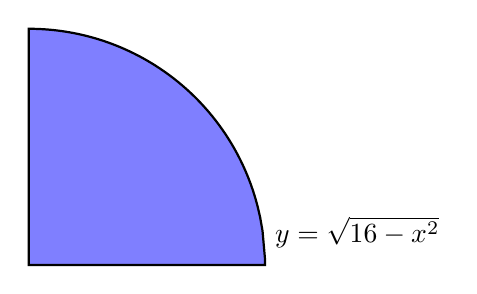
\begin{tikzpicture}
\YEaaxis{1}{6}{1}{4}
\draw[thick, fill=blue, fill opacity=0.5] plot[domain=0:3, samples=100] (\x,{sqrt(9-\x*\x)}) node[above right, opacity=1]{$y=\sqrt{16-x^2}$}--(3,0)--(0,0)--cycle;
\end{tikzpicture}
\end{center}
\end{solution}



\begin{Mquestion}[2016Q1]\label{1.1defintgeomb}
Use elementary geometry to calculate $\displaystyle \int_0^3 f(x)\,\,\dee{x}$, where
\begin{align*}
  f(x) = \begin{cases}
  x, & \text{if } x \le 1,\\
  1, & \text{if } x > 1.
  \end{cases}
\end{align*}

\end{Mquestion}

\begin{hint}
Sketch the graph of $f(x)$.
\end{hint}

\begin{answer}
$\displaystyle\int_0^3 f(x)\,\,\dee{x} = 2.5$
\end{answer}

\begin{solution}
Here is a sketch the graph of $f(x)$.

\begin{center}
    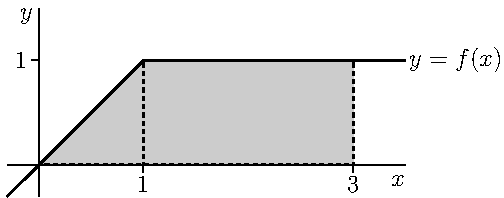
\includegraphics{OQ16_1}
\end{center}

\noindent
There is a linear increase from $x=0$ to $x=1$, followed by a constant. Using the interpretation of $\int_0^3 f(x)\,\,\dee{x}$ as the area between $y=f(x)$ and the
$x$--axis with $x$ between $0$ and $3$, we can break this area into:
\begin{itemize}
  \item $\int_0^1 f(x)\,\,\dee{x}$: a right-angled triangle of height $1$ and base $1$ and hence area $0.5$.
  \item $\int_1^3 f(x)\,\,\dee{x}$: a rectangle of height $1$ and base $2$ and hence
area $2$.
\end{itemize}
Summing up: $\int_0^3 f(x)\,\,\dee{x} = 2.5$.
\end{solution}
%%%%%%%%%%%%%%%%%%%




\begin{Mquestion}[2016Q1]\label{1.1cartime}
A car's gas pedal is applied at $t=0$ seconds and the car
accelerates continuously until $t=2$ seconds.
The car's speed at half-second intervals is given in the table
below.
Find the best possible \textbf{upper} estimate for the distance
that the car traveled during these two seconds.
\begin{center}
\renewcommand{\arraystretch}{1.3}
   \begin{tabular}{!{\vrule width 1pt}c!{\vrule width 1pt}c|c|c|c|c!{\vrule width 1pt}}
        \noalign{\hrule height 1pt}
        $t$ (s)  & $0$ & $0.5$ & $1.0$ & $1.5$ & $2$ \\    \hline
        $v$ (m/s) & 0 & 14 & 22 & 30 & 40 \\
      \noalign{\hrule height 1pt}
     \end{tabular}
\renewcommand{\arraystretch}{1.0}
\end{center}
\end{Mquestion}

\begin{hint}
At which time in the interval, for example, $0\le t\le 0.5$,  is the car moving
the fastest?
\end{hint}

\begin{answer}
53 m
\end{answer}

\begin{solution}
The car's speed increases with time. So its highest speed on any
time interval occurs at the right hand end of the interval and
the best possible upper estimate for the distance traveled is
given by the \emph{right} Riemann sum with $\Delta x =0.5$, which
is
\begin{equation*}
\big[v(0.5)+v(1.0)+v(1.5)+v(2.0)\big]\times 0.5
=\big[14+22+30+40\big]\times 0.5= 53\text{ m}
\end{equation*}
\end{solution}


\begin{Mquestion} True or false: the answer you gave for Question~\ref{1.1cartime} is definitely greater than or equal
to the distance the car travelled during the two seconds in question.
\end{Mquestion}
\begin{hint}
What are the possible speeds the car could have reached at time $t=0.25$?
\end{hint}
\begin{answer}
true
\end{answer}
\begin{solution}
There is a key detail in the statement of Question~\ref{1.1cartime}: namely, that the car is continuously accelerating. So, although we don't know exactly what's going on in between our brief snippets of information, we know that the car is not going any faster during an interval than at the end of that interval. Therefore, the car certainly travelled no farther than our estimation.

We ask this question in order to point out an important detail. If we did not have the information that the car was continuously accelerating, we would not be able to give a certain upper bound on its distance travelled. It would be possible that, when the car is not being observed (for example, when $t=0.25$), it is going much faster than when it is being observed.
\end{solution}



\begin{question}\label{1.1airtime}
An airplane's speed at one-hour intervals is given in the table below.
Approximate the distance travelled by the airplane from noon to 4pm three ways using a midpoint Riemann sum.
\begin{center}
\renewcommand{\arraystretch}{1.3}
   \begin{tabular}{!{\vrule width 1pt}c!{\vrule width 1pt}c|c|c|c|c!{\vrule width 1pt}}
        \noalign{\hrule height 1pt}
        time  & 12:00 pm & 1:00 pm & 2:00 pm & 3:00 pm & 4:00 pm   \\
         \hline
        speed (km/hr) & 800 & 700 & 850 &900 & 750 \\
      \noalign{\hrule height 1pt}
     \end{tabular}
\renewcommand{\arraystretch}{1.0}
\end{center}

\end{question}
\begin{hint}
You need to know the speed of the plane at the midpoints of your intervals, so (for example) noon to 1pm \emph{is not} one of your intervals.
\end{hint}
\begin{answer}
3200 km
\end{answer}
\begin{solution}
First, note that the distance travelled by the plane is equal to the area under the curve of its speed.

We need to know the speed of the plane at the midpoints of our intervals. So (for example) noon to 1pm \emph{is not} one of your intervals--we don't know the speed at 12:30. (A common idea is to average the two end values, 700 and 800. This is a fine approximation, but it is not a Riemann sum.) So, we use the two intervals 12:00 to 2:00, and 2:00 to 4:00. Then our intervals have length 2 hours, and at the midpoints of the intervals the speed of the plane is 700 kph and 900 kph, respectively. So, our midpoint Riemann sum gives us:
\[700(2)+900(2) = 3200\]
an approximation of 3200 km travelled by the plane from noon to 4:00 pm.

Remark: if we had been asked to approximate the distance travelled from 11:30 am to 4:30 pm, then we could have used the midpoint rule with five intervals and made use of every entry in the data table. With the question as stated, however, we ignore three out of five entries in the table because they are not the midpoints of our intervals.
\end{solution}


%%%%%%%%%%%%%%%%%%
\subsection*{\Application}
%%%%%%%%%%%%%%%%%%

\begin{Mquestion}[2016Q1]
\noindent (a)
Express
\begin{equation*}
\lim_{n\rightarrow\infty}
     \sum_{i=1}^n\frac{2}{n}\sqrt{4-\left(-2+\frac{2i}{n}\right)^2}
\end{equation*}
as a definite integal.

\noindent (b)
Evaluate the integral of part (a).
\end{Mquestion}

\begin{hint}
Sure looks like a Riemann sum.
\end{hint}

\begin{answer}
(a) There are many possible answers. Two are
        $\int_{-2}^0 \sqrt{4-x^2}\,\,\dee{x}$ and
        $\int_0^2 \sqrt{4-(-2+x)^2}\,\,\dee{x}$.
\noindent
(b) $\pi$
\end{answer}

\begin{solution}
\begin{description}
\item[Solution \#1:]
Set $x_i^*=-2+\frac{2i}{n}$. Then $a=x_0=-2$
and $b=x_n=0$ and $\Delta x=\frac{2}{n}$. So
\begin{align*}
\lim_{n\rightarrow\infty}
     \sum_{i=1}^n\frac{2}{n}\sqrt{4-\left(-2+\frac{2i}{n}\right)^2}
&= \lim_{n\rightarrow\infty}
     \sum_{i=1}^n f(x_i^*)\Delta x\qquad
   \text{ with $f(x) = \sqrt{4-x^2}$ and $\Delta x = \frac{2}{n}$ } \\
&=\int_{-2}^0 \sqrt{4-x^2}\,\,\dee{x}
\end{align*}

For the integral $\int_{-2}^0 \sqrt{4-x^2}\,\,\dee{x}$,
$y=\sqrt{4-x^2}$ is equivalent to $x^2+y^2=4$,
$y\ge 0$. So the integral represents the area between the upper
half of the circle $x^2+y^2=4$ (which has radius $2$)
and the $x$-axis with $-2\le x\le 0$, which is a quarter circle with area
$\frac{1}{4}\cdot \pi\, 2^2 = \pi$.

\begin{center}
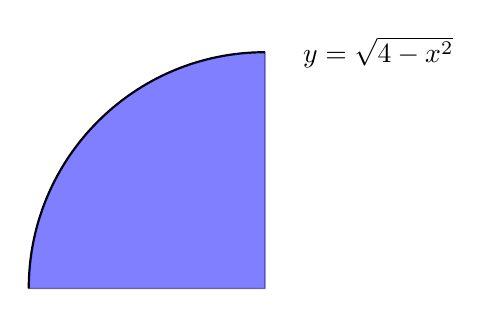
\begin{tikzpicture}
\YEaaxis{4}{1}{1}{3.5}
\draw[thick] (-3,0) arc (180:90:3cm) node[right]{\quad $y=\sqrt{4-x^2}$};
\draw[fill=blue, opacity=0.5] (-3,0) arc (180:90:3cm)--(0,0)--cycle;
\YExcoord{-3}{-{2}}
\end{tikzpicture}
\end{center}

\item[Solution \#2:]
Set $x_i^*=\frac{2i}{n}$. Then $a=x_0=0$
and $b=x_n=2$ and $\Delta x=\frac{2}{n}$. So
\begin{align*}
\lim_{n\rightarrow\infty}
     \sum_{i=1}^n\frac{2}{n}\sqrt{4-\left(-2+\frac{2i}{n}\right)^2}
&= \lim_{n\rightarrow\infty}
     \sum_{i=1}^n f(x_i^*)\Delta x\quad
   \text{ with $f(x) = \sqrt{4-(-2+x)^2}$, $\Delta x = \frac{2}{n}$ } \\
&=\int_0^2 \sqrt{4-(-2+x)^2}\,\,\dee{x}
\end{align*}

For the integral $\int_{0}^2  \sqrt{4-(-2+x)^2}\,\,\dee{x}$\ ,
$y=\sqrt{4-(x-2)^2}$ is equivalent to $(x-2)^2+y^2=4$,
$y\ge 0$. So the integral represents the area between the upper
half of the circle $(x-2)^2+y^2=4$ (which is centered at $(2,0)$ and has radius $2$)
and the $x$-axis with $0\le x\le 2$, which is a quarter circle with area
$\frac{1}{4}\cdot \pi\, 2^2 = \pi$.

\begin{center}
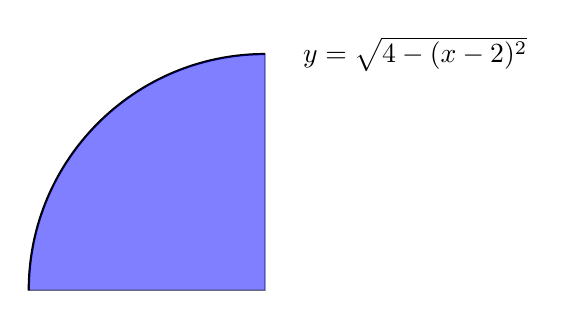
\begin{tikzpicture}
\YEaaxis{1}{4}{1}{3.5}
\draw[thick] (0,0) arc (180:90:3cm) node[right]{\quad $y=\sqrt{4-(x-2)^2}$};
\draw[fill=blue, opacity=0.5] (0,0) arc (180:90:3cm)--(3,0)--cycle;
\YExcoord{3}{{2}}
\end{tikzpicture}
\end{center}

\end{description}

\end{solution}
%%%%%%%%%%%%%%%%%%%%%%%%%%%%%%%%%%%%%%%

\begin{question}[2016Q1]
Consider the integral:
\begin{align*}
   \int_0^3 (7 + x^3) \,\,\dee{x} . ~~~~~~~~~ (*)
\end{align*}
\begin{enumerate} [(a)]
\item
   Approximate this integral using the left Riemann sum with $n=3$ intervals.
\item
    Write down the expression for the right Riemann sum with $n$
intervals and calculate the sum. Now take the limit $n \to \infty$
in your expression for the Riemann sum, to evaluate the integral
($*$) exactly.
\end{enumerate}
You may use the identity
\begin{align*}
\sum_{i=1}^{n} i^3 = \frac{n^4 +2n^3 + n^2}{4}
\end{align*}
\end{question}

\begin{hint}
For part (b): don't panic! Just take it one step at a time.
The first step is to write down the Riemann sum.
The second step is to evaluate the sum, using the given identity.
The third step is to evaluate the limit $n\rightarrow\infty$.
\end{hint}

\begin{answer}
(a) $30$
\qquad (b) $41 \frac{1}{4}$
\end{answer}

\begin{solution} (a)
The left Riemann sum is defined as
\begin{align*}
  L_n = \sum_{i=1}^{n}  f(x_{i-1})\Delta x
    \qquad\text{with }x_i=a+i\De x
\end{align*}
We subdivide into $n=3$ intervals, so that $\Delta x = \frac{b-a}{n}
=\frac{3-0}{3}=1$, $x_0=0$, $x_1=1$ and $x_2=2$.
The function $f(x) = 7 + x^3$ has the values
$f(x_0) = 7+0^3=7$,
$f(x_1) = 7+1^3=8$, and
$f(x_2) = 7+2^3=15$, from which we evaluate
\begin{align*}
L_3 = \big[f(x_0)+f(x_1)+f(x_2)\big]\De x = \big[7+8+15\big]\times 1= 30
\end{align*}

\noindent (b)
We divide into $n$ intervals so that
$\Delta x = \frac{b-a}{n}=\frac{3}{n}$ and  $x_i = a+i\De x= \frac{3i}{n}$.
The right Riemann sum is therefore:
\begin{align*}
R_n = \sum_{i=1}^{n}  f(x_i)\Delta x
    =  \sum_{i=1}^{n} \left[ 7 + \frac{(3i)^3}{n^3} \right] \frac{3}{n}
    =  \sum_{i=1}^{n} \left[ \frac{21}{n} + \frac{81\,i^3}{n^4} \right]
\end{align*}
To calculate the sum:
\begin{align*}
  R_n &= \left( \frac{21}{n} \sum_{i=1}^{n} 1 \right)
        +  \left( \frac{81}{n^4} \sum_{i=1}^{n} i^3 \right)\\
   &=\left( \frac{21}{n}\times n \right)+\left(  \frac{81}{n^4} \times \frac{n^4 +2n^3 + n^2}{4} \right)\\
                 &= 21 + \frac{81}{4}(1 +2/n + 1/n^2)
\end{align*}
To evaluate the limit exactly, we take $n \to \infty$. The expressions involving $1/n$ vanish leaving:
\begin{align*}
\int_0^3 (7 + x^3) \,\,\dee{x} = \lim_{n \to \infty} R_n = 21 + \frac{81}{4} = 41 \frac{1}{4}
\end{align*}

\end{solution}
%%%%%%%%%%%%%%%%%%%



\begin{question}[2013A]
Using a limit of right--endpoint Riemann
sums, evaluate $\displaystyle\int_2^4 x^2\ \,\dee{x}$. \\[5pt]
You may use the formulas
$\sum\limits_{i=1}^n i = \frac{n(n + 1)}{2}$ and
$\sum\limits_{i=1}^n i^2 = \frac{n(n + 1)(2n + 1)}{6}$.
\end{question}

\begin{hint}
The first step is to write down the Riemann sum.
The second step is to evaluate the sum, using the given formulas.
The third step is to evaluate the limit as $n\rightarrow\infty$.
\end{hint}

\begin{answer}
$\dfrac{56}{3}$
\end{answer}

\begin{solution}
In general, the right--endpoint Riemann sum
approximation to the integral $\int_a^b f(x)\,\,\dee{x}$ using $n$ rectangles is
\begin{align*}
\sum_{i=1}^n f(a+i\De x) \De x
\end{align*}
where $\De x=\frac{b-a}{n}$. In this problem, $a=2$, $b=4$, and $f(x)=x^2$,
so that $\De x=\frac{2}{n}$ and the  right--endpoint Riemann
sum approximation becomes
\begin{align*}
\sum_{i=1}^n f\Big(2+\frac{2i}{n}\Big) \frac{2}{n}&=
\sum_{i=1}^n \Big(2+\frac{2i}{n}\Big)^2 \frac{2}{n}\\
&=\sum_{i=1}^n \left(4+\frac{8i}{n}+\frac{4i^2}{n^2}\right)\frac{2}{n}
\\&=\sum_{i=1}^n \left(\frac{8}{n}+\frac{16i}{n^2}+\frac{8i^2}{n^3}\right)
\\&=\sum_{i=1}^n \frac{8}{n}+\sum_{i=1}^n \frac{16i}{n^2}
  +\sum_{i=1}^n \frac{8i^2}{n^3} \cr
&=\frac{8}{n}\sum_{i=1}^n 1+\frac{16}{n^2}\sum_{i=1}^n i
  +\frac{8}{n^3}\sum_{i=1}^n i^2\cr
&=\frac{8}{n}n + \frac{16}{n^2}\cdot\frac{n(n+1)}{2}
  +\frac{8}{n^3}\cdot\frac{n(n + 1)(2n + 1)}{6} \cr
&=8 + 8\Big(1+\frac{1}{n}\Big)
  +\frac{4}{3}\Big(1+\frac{1}{n}\Big)\Big(2+\frac{1}{n}\Big) \cr
\end{align*}
So
\begin{align*}
\int_2^4 x^2\ \,\dee{x}=\lim_{n\rightarrow\infty}
                      \Big[8 + 8\Big(1+\frac{1}{n}\Big)
                            +\frac{4}{3}\Big(1+\frac{1}{n}\Big)
                             \big(2+\frac{1}{n}\Big)\Big]
=8+8+\frac{4}{3}\times 2
=\frac{56}{3}
\end{align*}
\end{solution}
%%%%%%%%%%%%%%%%%%%

\begin{question}[2016Q1]
Find $\displaystyle\int_0^2 (x^3+x)\,\,\dee{x}$ using the definition of the definite integral.
You may use the summation formulas $\sum\limits_{i=1}^{n}i^3 = \frac{n^4+2n^3+n^2}4$ and
$\sum\limits_{i=1}^{n} i = \frac{n^2+n}{2}$.
\end{question}

\begin{hint}
The first step is to write down the Riemann sum.
The second step is to evaluate the sum, using the given formulas.
The third step is to evaluate the limit $n\rightarrow\infty$.
\end{hint}

\begin{answer}
$6$
\end{answer}

\begin{solution}
We'll use right Riemann sums with $a=0$ and $b=2$. When there are $n$ rectangles,
$\Delta x = \frac{b-a}{n}=\frac{2}{n}$ and  $x_i = a+i\De x=2i/n$.  So
we need to evaluate
\begin{align*}
\lim_{n\to\infty} \sum_{i=1}^{n} f(x_i)\De x
&=\lim_{n\to\infty} \sum_{i=1}^{n} \left( (x_i)^3 + x_i\right) \De x\\
  &=\lim_{n\to\infty} \sum_{i=1}^{n} \left( \left(\frac{2i}{n}\right)^3 + \frac{2i}{n}\right)
             \frac{2}{n} \\
   & = \lim_{n\to\infty} \frac{2}{n} \sum_{i=1}^{n} \left(\frac{8i^3}{n^3} + \frac{2i}{n}\right) \\
&= \lim_{n\to\infty} \left( \frac{16}{n^4} \sum_{i=1}^{n} i^3 + \frac{4}{n^2} \sum_{i=1}^{n} i \right) \\
   & = \lim_{n\to\infty} \left( \frac{16(n^4+2n^3+n^2)}{n^4 \cdot 4} + \frac{4(n^2+n)}{n^2 \cdot 2} \right) \\
&= \lim_{n\to\infty} \left( \frac{16}{4}\left(1+\frac{2}{n} + \frac1{n^2} \right) + \frac{4}{2}\left(1+\frac{1}{n}\right)\right) \\
& = \frac{16}{4} + \frac{4}{2} = 6.
\end{align*}
\end{solution}

%%%%%%%%%%%%%%%%%%%

\begin{Mquestion}[2014D]
Using a limit of right--endpoint Riemann sums, evaluate
$\displaystyle\int_1^4 (2x-1)\,\,\dee{x}$.
Do not use  anti-differentiation, except to check your answer.\footnote{You'll learn about this method starting in Section~\eref{CLP101}{sec fundamental} of the CLP-2 text.
You can also check this answer using geometry.}
You may use the formula $\sum\limits_{i=1}^{n} i = \frac{n(n+1)}{2}$.
\end{Mquestion}

\begin{hint}
You've probably seen this hint before. It is worth repeating.
Don't panic! Just take it one step at a time.
The first step is to write down the Riemann sum.
The second step is to evaluate the sum, using the given formula.
The third step is to evaluate the limit $n\rightarrow\infty$.
\end{hint}

\begin{answer}
$12$
\end{answer}

\begin{solution}
We'll use right Riemann sums with $a=1$, $b=4$ and $f(x) =2x-1$.
When there are $n$ rectangles, $\Delta x = \frac{b-a}{n}=\frac{3}{n}$ and
$x_i = a+i\De x=1 + 3i/n$.  So we need to evaluate
\begin{align*}
\lim_{n\to\infty} \sum_{i=1}^{n} f(x_i) \De x
& = \lim_{n\to\infty} \sum_{i=1}^{n} \left( 2x_i - 1\right) \De x\\
 & =\lim_{n\to\infty} \sum_{i=1}^{n} \left(2+ \frac{6i}{n}-1\right)\frac{3}{n} \\
& = \lim_{n\to\infty} \frac{3}{n} \sum_{i=1}^{n} \left(\frac{6i}{n}+1\right) \\
&= \lim_{n\to\infty} \left( \frac{18}{n^2} \sum_{i=1}^{n} i
                            + \frac{3}{n} \sum_{i=1}^{n} 1 \right) \\
& = \lim_{n\to\infty} \left(\frac{18\cdot n(n+1)}{n^2\cdot 2}
                              + \frac{3}{n}n\right)\\
&= \lim_{n\to\infty} \left(9\left(1+\frac{1}{n}\right) + 3\right) \\
& = 9 + 3 = 12.
\end{align*}
\end{solution}


\begin{question}
Give a function $f(x)$ that has the following expression as a right Riemann sum when $n=10$, $\Delta(x)=10$ and $a=-5$:
\[\sum_{i=1}^{10} 3(7+2i)^2\sin(4i)\,.\]
\end{question}
\begin{hint}
Using the definition of a right Riemann sum,  we can come up with an expression for
$f(-5+10i)$. In order to find $f(x)$, set $x=-5+10i$.
\end{hint}
\begin{answer}
$f(x)=\dfrac{3}{10}\left(\dfrac{x}{5}+8\right)^2\sin\left(\dfrac{2x}{5}+2\right)$
\end{answer}
\begin{solution}
Using the definition of a right Riemann sum,
\begin{align*}
\displaystyle\sum_{i=1}^{10} 3(7+2i)^2\sin(4i) &= \displaystyle\sum_{i=1}^{10} \Delta x f(a+i\Delta x)
\intertext{Since $\Delta x = 10$ and $a=-5$,}
\displaystyle\sum_{i=1}^{10} 3(7+2i)^2\sin(4i) &= \displaystyle\sum_{i=1}^{10} 10 f(-5+10i)
\intertext{Dividing both expressions by 10,}
\displaystyle\sum_{i=1}^{10} \frac{3}{10}(7+2i)^2\sin(4i) &= \displaystyle\sum_{i=1}^{10}  f(-5+10i)
\intertext{So, we have an expression for $f(-5+10i)$:}
f(-5+10i) &= \frac{3}{10}(7+2i)^2\sin(4i)
\intertext{In order to find $f(x)$, let $x=-5+10i$. Then $i=\frac{x}{10}+\frac{1}{2}$.}
f(x) &= \frac{3}{10}\left(7+2\left(\frac{x}{10}+\frac{1}{2}\right)\right)^2\sin\left(4\left(\frac{x}{10}+\frac{1}{2}\right)\right)\\
&=\frac{3}{10}\left(\frac{x}{5}+8\right)^2\sin\left(\frac{2x}{5}+2\right)\ .
\end{align*}
\end{solution}


\begin{question}\label{1.1_2x}
Using the method of Example~\eref{CLP101}{eg:INTexpareaB} in the CLP-2 text, evaluate
\[\int_0^1 2^x \ \dee{x}\]
\end{question}
\begin{hint}
Recall that for a positive constant $a$, $\diff{}{x}\left\{a^x\right\} = a^x \log a$, where $\log a$ is the natural logarithm (base $e$) of $a$.
\end{hint}
\begin{answer}
$\dfrac{1}{\log 2}$
\end{answer}
\begin{solution}
As in the text, we'll set up a Riemann sum for the given integral. Right Riemann sums have the simplest form, so we use a right Riemann sum, but we could equally well use left or midpoint.
\begin{align*}
\int_0^1 2^x\dee{x}&=\lim_{n \to \infty}\sum_{i=1}^n \Delta x f({a+i\Delta x})\\
&=\lim_{n \to \infty}\sum_{i=1}^n \frac{1}{n} f\left(\frac{i}{n}\right)\\
&=\lim_{n \to \infty}\sum_{i=1}^n  \frac{1}{n}\cdot 2^{i/n}\\
&=\lim_{n \to \infty}\frac{1}{n}\left(2^{1/n}+2^{2/n}+2^{3/n}+\cdots + 2^{n/n}\right)\\
&=\lim_{n \to \infty}\frac{2^{1/n}}{n}\left(1+2^{1/n}+2^{2/n}+\cdots + 2^{\frac{n-1}{n}}\right)\\
&=\lim_{n \to \infty}\frac{2^{1/n}}{n}\left(1+2^{1/n}+\left(2^{1/n}\right)^2+\cdots + \left(2^{1/n}\right)^{n-1}\right)
\intertext{The sum in parenthesis has the form of a geometric sum, with $r=2^{1/n}$:}
&=\lim_{n \to \infty}\frac{2^{1/n}}{n}\left(
\frac{\left(2^{1/n}\right)^n-1}{2^{1/n}-1}
\right)\\
&=\lim_{n \to \infty}\frac{2^{1/n}}{n}\left(
\frac{2-1}{2^{1/n}-1}
\right)\\
&=\lim_{n \to \infty}
\frac{2^{1/n}}{n(2^{1/n}-1)}
\intertext{Note as $n \to \infty$, $1/n \to 0$, so the numerator has limit 1, while the denominator has indeterminate form $\infty\cdot 0$. So, we'll do a little algebra to get this into a l'H\^opital-style indeterminate form:}
&=\lim_{n \to \infty}
\frac{\frac{1}{n}\cdot2^{1/n}}{2^{1/n}-1}
\\&=\lim_{n \to \infty}
\underbrace{\frac{\frac{1}{n}}{1-2^{-1/n}}}_{\atp{\mathrm{num}\to 0}{\mathrm{den}\to 0}}
\intertext{Now we can use l'H\^opital's rule. Recall $\diff{}{x}\left\{2^x\right\}=2^x\log x$, where $\log x$ is the natural logarithm of $x$, also sometimes written $\ln x$. We'll need to use the chain rule when we differentiate the denominator.}
&=\lim_{n \to \infty}
\frac{\frac{-1}{n^2}}{-2^{-1/n}\log 2 \cdot \frac{1}{n^2}}
\\&=\lim_{n \to \infty}
\frac{2^{1/n}}{\log 2}\\
&=\frac{1}{\log 2}
\end{align*}
Using a calculator, we see this is about 1.44 square units.
\end{solution}

\begin{question}
\begin{enumerate}[(a)]
\item Using the method of Example~\eref{CLP101}{eg:INTexpareaB} in the CLP-2 text, evaluate
\[\int_a^b 10^x \ \dee{x}\]
\item
\end{enumerate} Using your answer from above, make a guess for
\[\int_a^b c^x \ \dee{x}\]
where $c$ is a positive constant. Does this agree with Question~\ref{1.1_2x}?
\end{question}
\begin{hint}
Part (a) follows  the same pattern as Question~\ref{1.1_2x}--there's just a little more algebra involved, since our lower limit of integration is not 0.
\end{hint}
\begin{answer}
(a) $\dfrac{1}{\log 10}\left(10^b-10^a\right)$\\
(b) $\dfrac{1}{\log c}\left(c^b-c^a\right)$; yes, it agrees.
\end{answer}
\begin{solution}
As in the text, we'll set up a Riemann sum for the given integral. Right Riemann sums have the simplest form:
\begin{align*}
\int_a^b 10^x\dee{x}&=\lim_{n \to \infty}\sum_{i=1}^n \Delta x f({a+i\Delta x})\\
&=\lim_{n \to \infty}\sum_{i=1}^n \frac{b-a}{n} f\left(a+i\frac{b-a}{n}\right)\\
&=\lim_{n \to \infty}\sum_{i=1}^n  \frac{b-a}{n}\cdot 10^{a+i\frac{b-a}{n}}\\
&=\lim_{n \to \infty}\sum_{i=1}^n  \frac{b-a}{n}\cdot 10^a\cdot \left(10^{\frac{b-a}{n}}\right)^{i}\\
&=\lim_{n \to \infty} \frac{b-a}{n}\cdot 10^a\left(\left(10^{\frac{b-a}{n}}\right)^1+
\left(10^{\frac{b-a}{n}}\right)^2
+\left(10^{\frac{b-a}{n}}\right)^3
+\cdots + \left(10^{\frac{b-a}{n}}\right)^n
\right)\\
&=\lim_{n \to \infty} \frac{b-a}{n}
\cdot10^{a}\cdot10^{\frac{b-a}{n}}
\left(1+\left(10^{\frac{b-a}{n}}\right)+
\left(10^{\frac{b-a}{n}}\right)^2
+\cdots + \left(10^{\frac{b-a}{n}}\right)^{n-1}
\right)
\intertext{Now the sum in parentheses has the form of a geometric sum, with $r=10^{\frac{b-a}{n}}$:}
&=\lim_{n \to \infty}
\frac{b-a}{n}\cdot
10^{a}\cdot 10^{\frac{b-a}{n}}\left(
\frac{\left(10^{\frac{b-a}{n}}\right)^n-1}{10^{\frac{b-a}{n}}-1}
\right)\\
&=\lim_{n \to \infty}
\frac{\textcolor{blue}{b-a}}{n}\cdot
\textcolor{red}{10^{a}}\cdot 10^{\frac{b-a}{n}}\left(
\frac{\textcolor{purple}{10^{b-a}-1}}{10^{\frac{b-a}{n}}-1}
\right)
\intertext{The coloured parts do not depend on $n$, so for simplicity we can move them outside the limit.}
&=\textcolor{blue}{(b-a)}\cdot\textcolor{red}{10^a}\left(\textcolor{purple}{10^{b-a}-1}\right)\lim_{n \to \infty}
\frac{1}{n}\cdot
\left(
\frac{ 10^{\frac{b-a}{n}} }{10^{\frac{b-a}{n}}-1}
\right)
\\&={(b-a)}\cdot\left({10^{b}-10^a}\right)\lim_{n \to \infty}
\underbrace{\left(
\frac{ 1/n}{1-10^{-\frac{b-a}{n}}}
\right)}_{\atp{\mathrm{num}\to 0}{\mathrm{den}\to 0}}
\intertext{Now we can use l'H\^opital's rule. Recall $\diff{}{x}\left\{10^x\right\}=10^x\log x$, where $\log x$ is the natural logarithm of $x$, also sometimes written $\ln x$. For the denominator, we will have to use the chain rule.}
&={(b-a)}\cdot\left({10^{b}-10^a}\right)\lim_{n \to \infty}
\left(
\frac{ -1/n^2}{-10^{-\frac{b-a}{n}}\cdot \log 10 \cdot \frac{b-a}{n^2}}
\right)\\
&={(b-a)}\cdot\left({10^{b}-10^a}\right)\lim_{n \to \infty}
\left(
\frac{ 1}{10^{-\frac{b-a}{n}}\cdot \log 10 \cdot (b-a)}
\right)\\
&={(b-a)}\cdot\left({10^{b}-10^a}\right)
\left(
\frac{ 1}{ \log 10 \cdot (b-a)}
\right)\\
&=\frac{1}{\log 10}\left(10^b-10^a\right)
\end{align*}

For part (b), we can guess that if 10 were changed to $c$, our answer would be
\[\int_a^b c^x \ \dee{x}=\frac{1}{\log c}\left(c^b-c^a\right)\]
In Question~\ref{1.1_2x}, we had $a=0$, $b=1$, and $c=2$. In this case, the formula we guessed above gives
\[\int_0^1 2^x \ \dee{x}=\frac{1}{\log 2}\left(2^1-2^0\right)=\frac{1}{\log2}\]
This does indeed match the answer we calculated.

(In fact, we can directly show $\displaystyle\int_a^b c^x \ \dee{x}=\dfrac{1}{\log c}\left(c^b-c^a\right)$ using the method of this problem.)
\end{solution}


\begin{Mquestion}\label{1.1_awkwardcircle} Evaluate $\displaystyle\int_0^a \sqrt{1-x^2}\ \dee{x}$ using geometry, if $0
\leq a \leq 1$.
\end{Mquestion}
\begin{hint}
Your area can be divided into a section of a circle and a triangle. Then you can use geometry to find the area of each piece.
\end{hint}
\begin{answer}
$\frac{\pi}{4} -\frac{1}{2} \arccos(a) + \frac{1}{2}a\sqrt{1-a^2}$
\end{answer}
\begin{solution}
First, we note $y=\sqrt{1-x^2}$ is the upper half of a circle of radius 1, centred at the origin. We're taking the area under the curve from 0 to $a$, so the area in question is as shown in the picture below.

\begin{center}
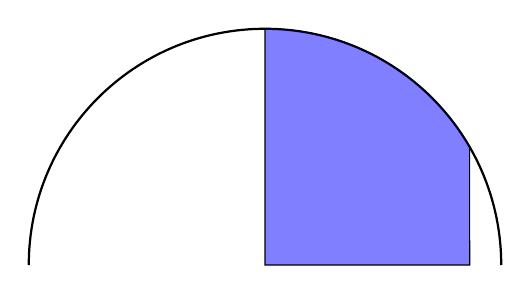
\begin{tikzpicture}
\YEaaxis{4}{4}{1}{4}
\YExcoord{-3}{-1}
\YExcoord{3}{1}
\YExcoord{2.6}{a}
\draw[thick] (-3,0) arc (180:0:3cm);
\draw[fill=blue, fill opacity=0.5] (0,0)--(0,3) arc(90:30:3cm)--(2.6,0)--cycle;
\end{tikzpicture}
\end{center}

In order to use geometry to find this area, we break it up into two pieces: a sector of a circle, and a triangle, shown below.

\begin{center}
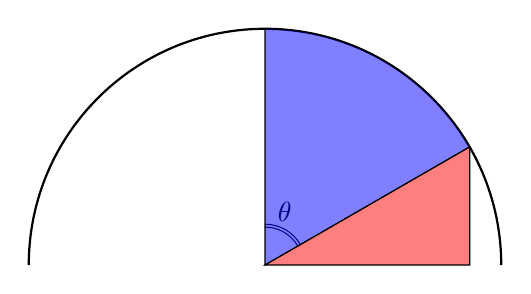
\begin{tikzpicture}
\YEaaxis{4}{4}{1}{4}
\YExcoord{-3}{-1}
\YExcoord{3}{1}
\YExcoord{2.6}{a}
\draw[thick] (-3,0) arc (180:0:3cm);
\draw[double](0,.5) arc (90:30:.5cm) node[midway, above]{$\theta$};
\draw[fill=blue, fill opacity=0.5] (0,0)--(0,3) arc(90:30:3cm)--cycle;
\draw[fill=red, fill opacity=0.5] (0,0)--(2.6,0)--(2.6,1.5)--cycle;
\end{tikzpicture}
\end{center}
\begin{description}
\item[Area of sector:] The sector is a portion of a circle with radius 1, with inner angle $\theta$. So, its area is $\frac{\theta}{2\pi}\left(\mbox{area of circle}\right) = \frac{\theta}{2\pi}\left(\pi\right) = \frac{\theta}{2}$.

Our job now is to find $\theta$ in terms of $a$. Note $\frac{\pi}{2}-\theta$ is the inner angle of the red triangle, which lies in the unit circle. So, $\cos\left(\frac{\pi}{2}-\theta\right)=a$. Then $\frac{\pi}{2}-\theta= \arccos(a)$, and so $\theta = \frac{\pi}{2} - \arccos(a)$.

Then the area of the sector is $\frac{\pi}{4} - \frac{1}{2}\arccos(a)$ square units.
\item[Area of triangle:] The triangle has base $a$. Its height is the $y$-value of the function when $x=a$, so its height is $\sqrt{1-a^2}$. Then the area of the triangle is $\frac{1}{2}a\sqrt{1-a^2}$.
\end{description}
We conclude $\displaystyle\int_0^a \sqrt{1-x^2}\ \dee{x} = \frac{\pi}{4} -\frac{1}{2} \arccos(a) + \frac{1}{2}a\sqrt{1-a^2}$.
\end{solution}



\begin{question}\label{1.1errornotaylor}
Suppose $f(x)$ is a positive, decreasing function from $x=a$ to $x=b$. You give an upper and lower bound on the area under the curve $y=f(x)$ using $n$ rectangles and a left and right Riemann sum, respectively, as in the picture below.

\begin{center}
\begin{tikzpicture}[scale=0.8]
\YEaaxis{1}{7.5}{1}{5}
\draw[red, pattern=crosshatch, pattern color=red] (1,0)--(1,4.25)-|(2,2.9)-|(3,1.85)-|(4,1.1)-|(5,0.65)-|(6,0.5)-|(6,0)--cycle;
\draw[thick] plot[domain=0.75:6.25, samples=100] (\x,{.15*(\x-6)*(\x-6)+.5}) node[right]{$y=f(x)$};
\draw[ fill=black, fill opacity=0.25] (1,0)--plot[domain=1:6, samples=100] (\x,{.15*(\x-6)*(\x-6)+.5}) --(6,0)--cycle;
\foreach \x in {1,...,6}{
\SUBTRACT{\x}{6}{\y}
\MULTIPLY{\y}{\y}{\z}
\MULTIPLY{\z}{0.15}{\w}
\ADD{\w}{0.5}{\c}
\draw[red, thick] (\x,0)--(\x,\c);}
\YExcoord{1}{a};
\YExcoord{6}{b};
\end{tikzpicture}
\hfill
\begin{tikzpicture}[scale=0.8]
\YEaaxis{1}{7.5}{1}{5}
\draw[red, pattern=crosshatch, pattern color=red] (1,0)--(1,2.9)-|(2,1.859)-|(3,1.1)-|(4,0.65)-|(5,0.5)-|(6,0)--cycle;
\draw[thick] plot[domain=0.75:6.25, samples=100] (\x,{.15*(\x-6)*(\x-6)+.5}) node[right]{$y=f(x)$};
\draw[fill=black, fill opacity=0.25] (1,0)--plot[domain=1:6, samples=100] (\x,{.15*(\x-6)*(\x-6)+.5}) --(6,0)--cycle;
\foreach \x in {2,...,6}{
\SUBTRACT{\x}{6}{\y}
\MULTIPLY{\y}{\y}{\z}
\MULTIPLY{\z}{0.15}{\w}
\ADD{\w}{0.5}{\c}
\draw[red, thick] (\x,0)--(\x,\c);}
\YExcoord{1}{a};
\YExcoord{6}{b};
\end{tikzpicture}
\end{center}
\begin{enumerate}[(a)]
\item\label{riemannerrorbounda} What is the difference between the lower bound and the upper bound? (That is, if we subtract the smaller estimate from the larger estimate, what do we get?) Give your answer in terms of $f$, $a$,  $b$, and $n$.
\item If you want to approximate the area under the curve to within 0.01 square units using this method, how many rectangles should you use? That is, what should $n$ be?
\end{enumerate}
\end{question}
\begin{hint}
\begin{enumerate}[(a)]
\item The difference between the upper and lower bounds is the area that is outside of the smaller rectangles but inside the larger rectangles.  Drawing both sets of rectangles on one picture might make things clearer. Look for an easy way to compute the area you want.
\item Use your answer from Part~(\ref{riemannerrorbounda}). Your answer will depend on $f$, $a$, and $b$.
\end{enumerate}
\end{hint}
\begin{answer}
\begin{enumerate}[(a)]
\item
$\left[f(b)-f(a)\right]\cdot\dfrac{b-a}{n}$
\item Choose $n$ to be an integer that is greater than or equal to $100\left[f(b)-f(a)\right](b-a)$.
\end{enumerate}
\end{answer}
\begin{solution}
\begin{enumerate}[(a)]
\item
The difference between our upper and lower bounds is the difference in areas between the larger set of rectangles and the smaller set of rectangles. Drawing them on a single picture makes this a little clearer.
\begin{center}
\begin{tikzpicture}
\YEaaxis{1}{7.5}{1}{5}
\draw[red, pattern=north east lines, pattern color=red] (1,0)--(1,4.25)-|(2,2.9)-|(3,1.85)-|(4,1.1)-|(5,0.65)-|(6,0.5)-|(6,0)--cycle;
\draw[purple, pattern=north west lines, pattern color=purple] (1,0)--(1,2.9)-|(2,1.859)-|(3,1.1)-|(4,0.65)-|(5,0.5)-|(6,0)--cycle;
\draw[thick] plot[domain=0.75:6.25, samples=100] (\x,{.15*(\x-6)*(\x-6)+.5}) node[right]{$y=f(x)$};
\foreach \x in {2,...,6}{
\SUBTRACT{\x}{6}{\y}
\MULTIPLY{\y}{\y}{\z}
\MULTIPLY{\z}{0.15}{\w}
\ADD{\w}{0.5}{\c}
\draw[purple, thick] (\x,0)--(\x,\c);}
\YExcoord{1}{a};
\YExcoord{6}{b};
\end{tikzpicture}
\end{center}

Each of the rectangles has width $\frac{b-a}{n}$, since we took a segment of the $x$-axis with length $b-a$ and chopped it into $n$ pieces. We could calculate the height of each rectangle, but it would be a little complicated, since it differs for each of them. An easier method is to notice that the area we want to calculate can be imagined as a single rectangle:

\begin{center}
\begin{tikzpicture}
\YEaaxis{1}{7.5}{1}{5}
\draw[thick] plot[domain=0.75:6.25, samples=100] (\x,{.15*(\x-6)*(\x-6)+.5}) node[right]{$y=f(x)$};
\YExcoord{1}{a};
\YExcoord{6}{b};
\draw[red, pattern=north east lines, pattern color=red] (1,4.25) rectangle (2,2.9) rectangle (3,1.85) rectangle (4,1.1) rectangle (5,0.65) rectangle (6,0.5);
\YEycoord{4.25}{f(a)}
\YEycoord{.5}{f(b)}
\draw[dotted] (0.2,4.25)--(1,4.25) (0.2,0.5)--(6,.5);
\draw[ultra thick, red, ->] (7,3) -- (9,3);

\draw[red, pattern=north east lines, pattern color=red] (11,4.25) rectangle (12,.5);
\foreach \y in {2.9,1.85,1.1,.65}{
	\draw[thick, red] (11,\y)--(12,\y);}
\end{tikzpicture}
\end{center}

The rectangle has base $\frac{b-a}{n}$. Its highest coordinate is $f(a)$, and its lowest is $f(b)$, so its height is $f(b)-f(a)$. Therefore, the difference in area between our lower bound and our upper bound is:
\[\left[f(b)-f(a)\right]\cdot\frac{b-a}{n}\]
\item We want to give a range with length at most 0.01, and guarantee that the area under the curve $y=f(x)$ is inside that range. In the previous part, we figured out that when we use $n$ rectangles, the length of our range is $\left[f(b)-f(a)\right]\cdot\frac{b-a}{n}$. So, all we have to do is set this to be less than or equal to 0.01, and solve for $n$:
\begin{align*}
\left[f(b)-f(a)\right]\cdot\frac{b-a}{n}&\leq 0.01 \\
100\left[f(b)-f(a)\right]\cdot(b-a)&\leq n
\end{align*}

We can choose $n$ to be an integer that is greater than or equal to $100\left[f(b)-f(a)\right]\cdot(b-a)$. Using that many rectangles, we find an upper and lower bound for the area under the curve. If we choose any number between our upper and lower bound as an approximation for the area under the curve, our error is no more than 0.01.
\end{enumerate}

Remark: this question depends on the fact that $f$ is decreasing and positive from $a$ to $b$. In general, bounding errors on approximations like this is not so straightforward.
\end{solution}


\begin{question}
Let $f(x)$ be a linear function,  let $a<b$ be integers, and let $n$ be a whole number. True or false: if we average the left and right Riemann sums for $\displaystyle\int_a^b f(x)\ \dee{x}$ using $n$ rectangles, we get the same value as the midpoint Riemann sum using $n$ rectangles.
\end{question}
\begin{hint}
Since $f(x)$ is linear, there exist real numbers $m$ and $c$ such that $f(x)=mx+c$. It's a little easier to first look at a single triangle from each sum, rather than the sums in their entirety.
\end{hint}
\begin{answer}
true (but note, for a non-linear function, it is possible that the midpoint Riemann sum is \emph{not} the average of the other two)
\end{answer}
\begin{solution}
Since $f(x)$ is linear, there exist real numbers $m$ and $c$ such that $f(x)=mx+c$. Now we can do some calculations. Suppose we have a rectangle in our Riemann sum that takes up the interval $[x,x+w]$.
\begin{itemize}
\color{blue} \item If we are using a left Riemann sum, our rectangle has height $f(x)=mx+c$.
Then it has area $w(mx+c)$. \color{red}
\item If we are using a right Riemann sum, our rectangle has height $f(x+w)=m(x+w)+c=mx+c+mw$. Then it has area $w(mx+c+mw)$.\color{black}
\item If we are using a midpoint Riemann sum, our rectangle has height $f(x+\frac{1}{2}w)=m(x+\frac{1}{2}w)+c=mx+c+\frac{1}{2}mw$.   Then it has area $w\left(mx+c+\frac{1}{2}w\right)$.
\end{itemize}
So, for each rectangle in our sums, the midpoint rectangle  has the same area as the average of the left and right rectangles:
\[w\left(mx+c+\frac{1}{2}mw\right) = \dfrac{\textcolor{blue}{w(mx+c)}+\textcolor{red}{w(mx+c+mw)}}{2}\]
It follows that the midpoint Riemann sum has a value equal to the average of the values of the left and right Riemann sums. To see this, let the rectangles in the midpoint Riemann sum have areas $M_1,M_2,\ldots,M_n$,
let the rectangles in the left Riemann sum have areas $\textcolor{blue}{L_1,L_2,\ldots,L_n}$, and
let the rectangles in the right Riemann sum have areas $\textcolor{red}{R_1,R_2,\ldots,R_n}$. Then the midpoint Riemann sum evaluates to $M_1+M_2+\cdots+M_n$, and:
\begin{align*}\dfrac{\textcolor{blue}{[L_1+L_2+\ldots+L_n]}+
\textcolor{red}{[R_1+R_2+\ldots+R_n]}
}{2} &=
\dfrac{\textcolor{blue}{L_1}+
\textcolor{red}{R_1}
}{2}+
\dfrac{\textcolor{blue}{L_2}+
\textcolor{red}{R_2}
}{2}+
\cdots
+
\dfrac{\textcolor{blue}{L_n}+
\textcolor{red}{R_n}
}{2} \\
&=M_1+M_2+\cdots+M_n\end{align*}
So, the statement is true.

(Note, however, it is false for many non-linear functions $f(x)$.)
\end{solution}

\section{Basic properties of the definite integral}
%
% Copyright 2018 Joel Feldman, Andrew Rechnitzer and Elyse Yeager.
% This work is licensed under a Creative Commons Attribution-NonCommercial-ShareAlike 4.0 International License.
% https://creativecommons.org/licenses/by-nc-sa/4.0/
%
\questionheader{ex:s1.2}

%%%%%%%%%%%%%%%%%%
\subsection*{\Conceptual}
%%%%%%%%%%%%%%%%%%
\begin{question}
For each of the following properties of definite integrals, draw a picture illustrating the concept, interpreting definite integrals as areas under a curve.

For simplicity, you may assume that $a \leq c \leq b$, and that $f(x),g(x)$ give positive values.
\begin{enumerate}[(a)]
\item $\displaystyle\int_a^a f(x)\,\dee{x}=0$\qquad
(Theorem~\eref{CLP101}{thm:Intdomain}.a in the CLP--II text)
\item $\displaystyle\int_a^b f(x)\,\dee{x}= \displaystyle\int_a^c f(x)\,\dee{x} + \int_c^b f(x)\dee{x} $\qquad (Theorem~\eref{CLP101}{thm:Intdomain}.c in the CLP--II text)
\item $\displaystyle\int_a^b \left( f(x) + g(x) \right)\,\dee{x}
= \displaystyle\int_a^b f(x)\,\dee{x} + \displaystyle\int_a^b g(x)\,\dee{x}$\qquad (Theorem~\eref{CLP101}{thm:Intarith}.a  in the CLP--II text)
\end{enumerate}
\end{question}
\begin{hint}
\begin{enumerate}[(a)]
\item What is the length of this figure?
\item Think about cutting the area into two pieces vertically.
\item Think about cutting the area into two pieces another way.
\end{enumerate}
\end{hint}
\begin{answer}
Possible drawings:
\begin{center}
\begin{tikzpicture}
\YEaaxis{1}{2.5}{1}{3}
\YExcoord{1}{a}
\draw[thick] plot[domain=-.5:2] (\x,{\x*\x/2+.25}) node[right] {$y=f(x)$};
\draw[thick, blue] (1,0)--(1,.75);
\end{tikzpicture}
\hfill
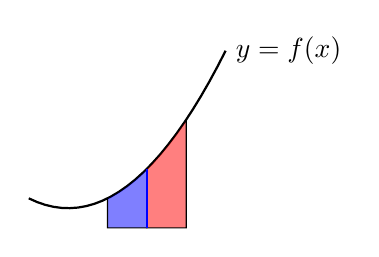
\begin{tikzpicture}
\YEaaxis{1}{2.5}{1}{3}
\YExcoord{.5}{a}
\YExcoord{1}{c}
\YExcoord{1.5}{b}
\draw[thick] plot[domain=-.5:2] (\x,{\x*\x/2+.25}) node[right] {$y=f(x)$};

\draw[fill=blue, fill opacity=0.5] plot[domain=.5:1] (\x,{\x*\x/2+.25})--(1,.75)--(1,0)--(.5,0)--cycle;
\draw[fill=red, fill opacity=0.5] plot[domain=1:1.5] (\x,{\x*\x/2+.25})--(1.5,1.375)--(1.5,0)--(1,0)--cycle;

\draw[thick, blue] (1,0)--(1,.75);
\end{tikzpicture}
\hfill\begin{tikzpicture}
\YEaaxis{1}{2.5}{1}{3}
\YExcoord{.5}{a}
\YExcoord{1.5}{b}
\draw[thick] plot[domain=-.5:2] (\x,{\x*\x/3+.25}) node[right] {$y=f(x)$};
\draw[thick] plot[domain=-.5:2] (\x,{2+\x/2-\x*\x/10}) node[right] {$y=f(x)+g(x)$};
\draw[fill=blue, fill opacity=0.5] plot[domain=.5:1.5] (\x,{\x*\x/3+.25})--(1.5,0)--(.5,0)--cycle;
\draw[fill=red, fill opacity=0.5]plot[domain=.5:1.5] (\x,{2+\x/2-\x*\x/10})--
plot[domain=1.5:.5] (\x,{\x*\x/3+.25}) --cycle;
\end{tikzpicture}
\end{center}

\end{answer}
\begin{solution}
\begin{enumerate}[(a)]
\item $\displaystyle\int_a^a f(x)\,\dee{x}=0$
\begin{center}
\begin{tikzpicture}
\YEaaxis{1}{2.5}{1}{2}
\YExcoord{1}{a}
\draw[thick] plot[domain=-.5:2] (\x,{\x*\x/2+.25}) node[right] {$y=f(x)$};
\draw[thick, blue] (1,0)--(1,.75);
\end{tikzpicture}
\end{center}
The area under the curve is zero, because it's a region with no width.

\item $\displaystyle\int_a^b f(x)\,\dee{x}=\textcolor{blue}{ \displaystyle\int_a^c f(x)\,\dee{x}} +\textcolor{red}{ \int_c^b f(x)\dee{x} }$

\begin{center}
\begin{tikzpicture}
\YEaaxis{1}{2.5}{1}{2}
\YExcoord{.5}{a}
\YExcoord{1}{c}
\YExcoord{1.5}{b}
\draw[thick] plot[domain=-.5:2] (\x,{\x*\x/2+.25}) node[right] {$y=f(x)$};

\draw[fill=blue, fill opacity=0.5] plot[domain=.5:1] (\x,{\x*\x/2+.25})--(1,.75)--(1,0)--(.5,0)--cycle;
\draw[fill=red, fill opacity=0.5] plot[domain=1:1.5] (\x,{\x*\x/2+.25})--(1.5,1.375)--(1.5,0)--(1,0)--cycle;

\draw[thick, blue] (1,0)--(1,.75);
\end{tikzpicture}
\end{center}

If we assume $a \leq c \leq b$, then this identity simply tells us that  if we add up the area under the curve from $a$ to $c$, and from $c$ to $b$, then we get the whole area under the curve from $a$ to $b$.

(The situation is slightly more complicated when $c$ is not between $a$ and $b$, but it still works out.)

\item $\displaystyle\int_a^b \left( f(x) + g(x) \right)\,\dee{x}
=\textcolor{blue}{ \displaystyle\int_a^b f(x)\,\dee{x}} +\textcolor{red}{ \displaystyle\int_a^b g(x)\,\dee{x}}$

\begin{center}
\begin{tikzpicture}
\YEaaxis{1}{2.5}{1}{3}
\YExcoord{.5}{a}
\YExcoord{1.5}{b}
\draw[thick] plot[domain=-.5:2] (\x,{\x*\x/3+.25}) node[right] {$y=f(x)$};
\draw[thick] plot[domain=-.5:2] (\x,{2+\x/2-\x*\x/10}) node[right] {$y=f(x)+g(x)$};
\draw[fill=blue, fill opacity=0.5] plot[domain=.5:1.5] (\x,{\x*\x/3+.25})--(1.5,0)--(.5,0)--cycle;
\draw[fill=red, fill opacity=0.5]plot[domain=.5:1.5] (\x,{2+\x/2-\x*\x/10})--
plot[domain=1.5:.5] (\x,{\x*\x/3+.25}) --cycle;
\end{tikzpicture}
\end{center}

The blue-shaded area in the picture above is $\displaystyle\int_a^b f(x)\ \dee{x}$. The area under the curve $f(x)+g(x)$ but above the curve $f(x)$ (shown in red) is $\displaystyle\int_a^b g(x)\ \dee{x}$.
\end{enumerate}\end{solution}


\begin{Mquestion} If $\displaystyle\int_0^b \cos x\ \dee{x}=\sin b$, then what is $\displaystyle\int_a^b \cos x\
\dee{x}$?
\end{Mquestion}
\begin{hint}
Use the identity $\int\limits_a^b f(x)\ \dee{x} =
\int\limits_a^c f(x)\ \dee{x}+
\int\limits_c^b f(x)\ \dee{x}$.
\end{hint}
\begin{answer}
$\sin b-\sin a$
\end{answer}
\begin{solution}
Using the identity
\begin{align*}
\int\limits_a^b f(x)\ \dee{x} &=
\int\limits_a^c f(x)\ \dee{x}+
\int\limits_c^b f(x)\ \dee{x}\ ,
\intertext{ we see}
\int\limits_a^b\cos x\ \dee{x} &=
\int\limits_a^0 \cos x\ \dee{x}+
\int\limits_0^b \cos x\ \dee{x}\\&=
-\int\limits_0^a \cos x\ \dee{x}+
\int\limits_0^b \cos x\ \dee{x}\\
&=-\sin a + \sin b\\
&=\sin b - \sin a
\end{align*}
\end{solution}

\begin{Mquestion}[2015A, 2016A]
Decide whether each of the following statements is true or false.
If false, provide a counterexample. If true, provide a brief justification.
(Assume that $f(x)$ and $g(x)$ are continuous functions.)

\begin{enumerate}[(a)]
\item
$\displaystyle\int_{-3}^{-2} f(x) \dee{x}=-\displaystyle\int_{3}^{2} f(x) \dee{x}$.\item
If $f(x)$ is an odd function, then $\displaystyle \int_{-3}^{-2} f(x)\,\dee{x} = \int_2^3 f(x)\,\dee{x}$.
\item
$\displaystyle\int_{0}^{1} f(x)\cdot g(x) ~\dee{x}
   =\int_{0}^{1} f(x) ~\dee{x} \cdot \int_{0}^{1} g(x) ~\dee{x}$.
\end{enumerate}
\end{Mquestion}

%\begin{hint}
%\end{hint}

\begin{answer}
(a) False. For example, the function
\begin{align*}
f(x) = \begin{cases}
               0 & \text{for $x<0$} \\
               1 & \text{for $x\ge0$}
      \end{cases}
\end{align*}
provides a counterexample.

\noindent (b)
False. For example, the function $f(x)=x$ provides a counterexample.

\noindent (c)
False. For example, the functions
\begin{align*}
f(x) = \begin{cases}
               0 & \text{for $x<\frac{1}{2}$} \\
               1 & \text{for $x\ge\frac{1}{2}$}
      \end{cases}
&&\mbox{and}&&g(x) = \begin{cases}
               0 & \text{for $x\ge \frac{1}{2}$} \\
               1 & \text{for $x<\frac{1}{2}$}
      \end{cases}
\end{align*}


 provide a counterexample.


\end{answer}

\begin{solution} (a)
False. For example if
\begin{align*}
f(x) = \begin{cases}
               0 & \text{for $x<0$} \\
               1 & \text{for $x\ge0$}
      \end{cases}
\end{align*}
then \textcolor{blue}{$\int_{-3}^{-2} f(x) \dee{x}=0$} and \textcolor{red}{$-\int_{3}^{2} f(x) \dee{x}=-1$}.

\begin{center}
\begin{tikzpicture}
\YEaaxis{2.5}{2.5}{.5}{1.25}
\draw[thick] (-2.25,0)--(0,0) node[opendot]{};
\draw[thick] (0,1)node[vertex]{}--(2.25,1) ;
\YExcoord{-2}{-3}
\YExcoord{-1.33}{-2}
\YExcoord{2}{3}
\YExcoord{1.33}{2}
\draw[ultra thick, blue] (-2,0)--(-1.33,0);
\draw[red, thick, fill=red, fill opacity=0.5] (1.33,0) rectangle (2,1);
\end{tikzpicture}
\end{center}

\noindent (b)
False.  For example, if $f(x)=x$, then \textcolor{blue}{$\int_{-3}^{-2} f(x)\,\dee{x} $} is negative while
\textcolor{red}{$\int_2^3 f(x)\,\dee{x} $} is positive, so they cannot be the same.


\begin{center}
\begin{tikzpicture}
\YEaxis{2.5}{2.5}
\draw[thick] (-2.25,-2.25)--(2.25,2.25);
\YEnxcoord{-2}{-3}
\YEnxcoord{-1.33}{-2}
\YExcoord{2}{3}
\YExcoord{1.33}{2}
\draw[thick, blue, fill=blue, fill opacity=0.5] (-2,-2)--(-1.33,-1.33)|-(-2,0)--cycle;
\draw[red, thick, fill=red, fill opacity=0.5] (1.33,1.33) --(2,2)|-(1.33,0)--cycle;
\end{tikzpicture}
\end{center}


\noindent (c)
False.  For example, consider the functions
\begin{align*}
f(x) = \begin{cases}
               0 & \text{for $x<\frac{1}{2}$} \\
               1 & \text{for $x\ge\frac{1}{2}$}
      \end{cases}
&&\mbox{and}&&g(x) = \begin{cases}
               0 & \text{for $x\ge \frac{1}{2}$} \\
               1 & \text{for $x<\frac{1}{2}$}
      \end{cases}
\end{align*}

Then $f(x)\cdot g(x)=0$ for all $x$, so $\int_0^1 f(x)\cdot g(x) \dee{x}=0$. However,
\textcolor{blue}{$\int_0^1 f(x) \dee{x}= \frac{1}{2}$} and \textcolor{red}{$\int_0^1 g(x) \dee{x}= \frac{1}{2}$}, so $\int_0^1 f(x)\dee{x} \cdot \int_0^1 g(x) \dee{x}= \frac{1}{4}$.

\begin{center}
\begin{tikzpicture}
\YExcoord{1}{\frac{1}{2}}
\YExcoord{2}{1}
\YEycoord{1}{1}
\YEaaxis{.5}{2.5}{.5}{1.25}
\draw[blue, fill=blue, fill opacity=0.5] (1,1)rectangle (2,0);
\draw[thick] (-.25,0)--(1,0) node[opendot]{};
\draw[thick] (1,1)node[vertex]{}--(2.25,1)  node[right]{$f(x)$};
\end{tikzpicture}
\hspace{2cm}
\begin{tikzpicture}
\YExcoord{1}{\frac{1}{2}}
\YExcoord{2}{1}
\YEycoord{1}{1}
\YEaaxis{.5}{2.5}{.5}{1.25}
\draw[red, fill=red, fill opacity=0.5] (0,1)rectangle (1,0);
\draw[thick] (1,0)node[vertex]{}--(2.25,0)  node[above]{$g(x)$};
\draw[thick] (-.25,1)--(1,1) node[opendot]{};
\end{tikzpicture}
\end{center}

\end{solution}
%%%%%%%%%%%%%%%%%%%


\begin{question}
Suppose we want to make a right Riemann sum with 100 intervals to approximate $\int\limits_5^0 f(x)\ \dee{x}$, where $f(x)$ is a function that gives only positive values.\\[5pt]
\begin{enumerate}[(a)]
\item What is $\Delta x$?
\item Are the heights of our rectangles positive or negative?
\item Is our Riemann sum positive or negative?
\item Is the signed area under the curve $y=f(x)$ from $x=0$ to $x=5$ positive or negative?
\end{enumerate}
\end{question}
\begin{hint}
Note that the limits of the integral given are in the opposite order from what we might expect: the smaller number is the top limit of integration.

Recall $\De x = \frac{b-a}{n}$.
\end{hint}
\begin{answer}
(a) $-\dfrac{1}{20}$
\qquad
(b) positive
\qquad
(c) negative
\qquad
(d) positive

\end{answer}
\begin{solution}
\begin{enumerate}[(a)]
\item $\Delta x = \dfrac{b-a}{n}=\dfrac{0-5}{100} = -\dfrac{1}{20}$

Note: if we were to use the Riemann-sum definition of a definite integral, this is how we would justify the identity $\int\limits_a^b f(x)\dee{x}=-\int\limits_b^a f(x)\dee{x}$.

\item The heights of the rectangles are given by $f(x_i)$, where $x_i = a+i\Delta x = 5 - \frac{i}{20}$. Since $f(x)$ only gives positive values, $f(x_i) >0$, so the heights of the rectangles are positive.

\item Our Riemann sum is the sum of the signed areas of individual rectangles. Each rectangle has a negative base ($\Delta x$) and a positive height ($f(x_i)$).  So, each term of our sum is negative. If we add up negative numbers, the sum is negative. So, the Riemann sum is negative.
\item Since $f(x)$ is always above the $x$-axis, $\int\limits_0^5 f(x)\dee{x}$ is positive.
\end{enumerate}

\end{solution}


%%%%%%%%%%%%%%%%%%
\subsection*{\Procedural}
%%%%%%%%%%%%%%%%%%

\begin{question}[M105 2015A]
Suppose $\displaystyle\int_2^3 f(x)\,\dee{x} = -1$ and
$\displaystyle\int_2^3 g(x)\,\dee{x} = 5$. Evaluate
$\displaystyle \int_2^3 \big( 6 f(x) - 3 g(x) \big)\,\dee{x}$.
\end{question}

\begin{hint}
Split the ``target integral'' up into pieces that can be evaluated using the given integrals.
\end{hint}

\begin{answer}
$-21$
\end{answer}

\begin{solution}
The operation of integration is linear (that's
part (d) of the ``arithmetic of integration''
Theorem  \eref{CLP101}{thm:Intarith} in the CLP--II text),
so that:
\begin{align*}
\int_2^3 [6 f(x) -3 g(x)]\,\dee{x}
&= \int_2^3 6 f(x)\,\dee{x}  - \int_2^3 3 g(x)\,\dee{x} \\
&= 6 \int_2^3  f(x)\,\dee{x}  - 3\int_2^3 g(x)\,\dee{x}
= (6 \times (-1)) - (3 \times 5)
= -21
\end{align*}

\end{solution}


\begin{question}[2016Q1]
If $\displaystyle\int_0^2 f(x)\,\dee{x} = 3$ and
$\displaystyle\int_0^2 g(x)\,\dee{x} = -4$, calculate
$\displaystyle \int_0^2 \big( 2 f(x) + 3 g(x) \big)\,\dee{x}$.
\end{question}

\begin{hint}
Split the ``target integral'' up into pieces that can be evaluated using the given integrals.
\end{hint}

\begin{answer}
$-6$
\end{answer}

\begin{solution}
The operation of integration is linear (that's
part (d) of the ``arithmetic of integration''
Theorem  \eref{CLP101}{thm:Intarith} in the CLP--II text),
so that:
\begin{align*}
\int_0^2 [2 f(x) +3 g(x)]\,\dee{x}
   &= \int_0^2 2 f(x)\,\dee{x}  + \int_0^2 3 g(x)\,\dee{x} \\
&= 2 \int_0^2  f(x)\,\dee{x}  + 3\int_0^2 g(x)\,\dee{x} = (2 \times 3) + (3 \times (-4)) = -6
\end{align*}

\end{solution}


\begin{Mquestion}[2016Q1]
 The functions $f(x)$ and $g(x)$ obey
\begin{equation*}
\int_0^{-1} f(x)\,\dee{x} = 1 \qquad
\int_0^2 f(x)\,\dee{x} = 2 \qquad
\int_{-1}^0 g(x)\,\dee{x} = 3 \qquad
\int_0^2 g(x)\,\dee{x} = 4
\end{equation*}
Find $\int_{-1}^2 \big[3g(x)-f(x)\big]\,\dee{x}$.
\end{Mquestion}

\begin{hint}
Split the ``target integral'' up into pieces that can be evaluated using the given integrals.
\end{hint}

\begin{answer}
20
\end{answer}

\begin{solution}
Using part (d) of the ``arithmetic of integration'' Theorem  \eref{CLP101}{thm:Intarith},
followed by parts (c) and (b) of the ``arithmetic for the domain of integration'' Theorem
  \eref{CLP101}{thm:Intdomain} in the
%\href{http://www.math.ubc.ca/%7Efeldman/m101/clp/clp_notes_101.pdf}{CLP 101 notes}.
 in the CLP--II text,
\begin{align*}
\int_{-1}^2 \big[3g(x)-f(x)\big]\,\dee{x}
&=3\int_{-1}^2 g(x)\,\dee{x}-\int_{-1}^2 f(x)\,\dee{x} \\
&=3\int_{-1}^0 g(x)\,\dee{x}+3\int_0^2 g(x)\,\dee{x}
-\int_{-1}^0 f(x)\,\dee{x}-\int_0^2 f(x)\,\dee{x} \\
&=3\int^0_{-1} g(x)\,\dee{x}+3\int_0^2 g(x)\,\dee{x}
+\int_0^{-1} f(x)\,\dee{x}-\int_0^2 f(x)\,\dee{x} \\
&=3\times 3+3\times 4 + 1 - 2 = 20
\end{align*}

\end{solution}
%%%%%%%%%%%%%%%%%%%%%%%%
\begin{question} In Question~\ref{1.1_awkwardcircle}, Section 1.1, we found that
\[\int_0^a\sqrt{1-x^2}\ \dee{x}=\frac{\pi}{4} - \frac{1}{2}\arccos(a)+\frac{1}{2}a\sqrt{1-a^2}\]
when $0\le a\le 1$.

Using this fact, evaluate the following:
\begin{enumerate}[(a)]
\item $\displaystyle\int_{a}^0 \sqrt{1-x^2}\ \dee{x}$, where $-1 \leq a \leq 0$
\item $\displaystyle\int_{a}^1 \sqrt{1-x^2}\ \dee{x}$, where $0 \leq a \leq 1$
\end{enumerate}
\end{question}
\begin{hint} For part (a), use the symmetry of the integrand. For part (b), the area $\int	\limits_{0}^1 \sqrt{1-x^2}\ \dee{x}$ is easy to find--how is this useful to you?
\end{hint}
\begin{answer}
\begin{enumerate}[(a)]
\item $\frac{\pi}{4} - \frac{1}{2}\arccos(-a)-\frac{1}{2}a\sqrt{1-a^2}$
\item $\frac{1}{2}\arccos(a)-\frac{1}{2}a\sqrt{1-a^2}$
\end{enumerate}
\end{answer}
\begin{solution}
\begin{enumerate}[(a)]
\item Since $\sqrt{1-x^2}$ is an even function,
\begin{align*}
\displaystyle\int_{a}^0 \sqrt{1-x^2}\ \dee{x} &=\displaystyle\int_{0}^{|a|} \sqrt{1-x^2}\ \dee{x}  = \frac{\pi}{4} - \frac{1}{2}\arccos(|a|)+\frac{1}{2}|a|\sqrt{1-|a|^2}\\
&=\frac{\pi}{4} - \frac{1}{2}\arccos(-a)-\frac{1}{2}a\sqrt{1-a^2}
\end{align*}
\item Note $\displaystyle\int_{0}^1 \sqrt{1-x^2}\ \dee{x}=\frac{\pi}{4}$, since the area under the curve represents one-quarter of the unit circle. Then,
\begin{align*}\displaystyle\int_{a}^1 \sqrt{1-x^2}\ \dee{x}&=
\displaystyle\int_{0}^1 \sqrt{1-x^2}\ \dee{x}-
\displaystyle\int_{0}^a \sqrt{1-x^2}\ \dee{x}\\
&=\frac{\pi}{4}-\left(\frac{\pi}{4} - \frac{1}{2}\arccos(a)+\frac{1}{2}a\sqrt{1-a^2}\right)\\
&=\frac{1}{2}\arccos(a)-\frac{1}{2}a\sqrt{1-a^2}
\end{align*}
\end{enumerate}

\end{solution}


%%%%%%%%%%%%%%%%%%%%%%%%

\begin{Mquestion}[M105 2013A]\label{prob:s1.2_2}
Evaluate ${\displaystyle\int_{-1}^2 |2x|\ \dee{x}}$.

You may use the result from  Example \eref{CLP101}{eg:INTPROPx}  in the CLP--II text
that
$
\int\limits_a^b x\ \dee{x}=\frac{b^2-a^2}{2}
$.

\end{Mquestion}

\begin{hint}
The evaluation of this integral was also the subject of Question
\ref{prob:s1.2_2} in Section 1.1. This time try using the method
of Example \eref{CLP101}{eg:INTPROPabs} in the
%\href{http://www.math.ubc.ca/%7Efeldman/m101/clp/clp_notes_101.pdf}{CLP 101 notes}.
CLP--II text.
\end{hint}

\begin{answer}
$5$
\end{answer}

\begin{solution}
Recall that
\begin{align*}
|x|=\begin{cases} -x &\text{if $x\le 0$}\\
                   x &\text{if $x\ge 0$}
    \end{cases}
\end{align*}
so that
\begin{align*}
|2x|=\begin{cases} -2x &\text{if $x\le 0$}\\
                    2x &\text{if $x\ge 0$}
    \end{cases}
\end{align*}
Also recall, from  Example \eref{CLP101}{eg:INTPROPx} in the
%\href{http://www.math.ubc.ca/%7Efeldman/m101/clp/clp_notes_101.pdf}{CLP 101 notes}.
CLP--II text that
\begin{align*}
\int_a^b x\ \dee{x}&=\frac{b^2-a^2}{2}
\end{align*}
So
\begin{align*}
\int_{-1}^2 |2x|\ \dee{x}
&=\int_{-1}^0 |2x|\ \dee{x}+\int_0^2 |2x|\ \dee{x}
=\int_{-1}^0 (-2x)\ \dee{x}+\int_0^2 2x\ \dee{x} \\
&= -2\int_{-1}^0 x\ \dee{x}+2\int_0^2 x\ \dee{x}
=-2\cdot\frac{0^2-(-1)^2}{2} +2\cdot\frac{2^2-0^2}{2} \\
&=1+4=5
\end{align*}


\end{solution}
%%%%%%%%%%%%%%%%%%%



\begin{question}
Evaluate $\displaystyle\int_{-5}^5 x|x|\ \dee{x}$\,.
\end{question}
\begin{hint} Use symmetry.
\end{hint}
\begin{answer} 0
\end{answer}
\begin{solution}
We note that the integrand $f(x)=x|x|$ is an odd function, because $f(-x)=-x|-x|=-x|x|=-f(x)$. Then, by Theorem~\eref{CLP101}{thm:INTevenodd}.b in the CLP--II text,
 $\displaystyle\int_{-5}^5 x|x| \ \dee{x}=0$.
\end{solution}

\begin{Mquestion}
Suppose $f(x)$ is an even function and $\displaystyle\int_{-2}^2 f(x)\dee{x}=10$. What is
$\displaystyle\int_{-2}^0 f(x)\dee{x}$?
\end{Mquestion}
\begin{hint}
Check Theorem~\eref{CLP101}{thm:INTevenodd} in the CLP--II text.
\end{hint}
\begin{answer} 5
\end{answer}
\begin{solution}
Using Theorem~\eref{CLP101}{thm:INTevenodd}.a in the CLP--II text,
\begin{align*}10&=\int_{-2}^2 f(x)\dee{x}=2\int_{0}^2f(x)\dee{x}\\
5&=\int_{0}^2f(x)\dee{x}
\intertext{Also,}
\int_{-2}^2 f(x)\dee{x}&=\int_{-2}^0 f(x)\dee{x}+\int_{0}^2 f(x)\dee{x}
\intertext{So,}
\int_{-2}^0 f(x)\dee{x}&=\int_{-2}^2 f(x)\dee{x}-\int_{0}^2 f(x)\dee{x}\\
&=10-5=5
\end{align*}
Indeed, for any even function $f(x)$, $\int\limits_{-a}^0 f(x)\dee{x} = \int\limits_{0}^a f(x)\dee{x}$.
\end{solution}

%%%%%%%%%%%%%%%%%%
\subsection*{\Application}
%%%%%%%%%%%%%%%%%%

\begin{question}[2016Q1]
Evaluate $\displaystyle\int_{-2}^{2} \left(5+\sqrt{4-x^2}\right)\dee{x}$.
\end{question}

\begin{hint}
Split the integral into a sum of two integrals. Interpret each geometrically.
\end{hint}

\begin{answer}
$20 +2\pi$
\end{answer}

\begin{solution}
We first use additivity:
\begin{align*}
 \int_{-2}^{2} \left(5+\sqrt{4-x^2}\right)\dee{x} =
\textcolor{blue}{  \int_{-2}^{2} 5\,\dee{x} }+ \textcolor{red}{\int_{-2}^{2} \sqrt{4-x^2}\,\dee{x}}
\end{align*}
The first integral represents the area of a rectangle of height 5 and width 4 and so equals $20$.
The second integral represents the area above the $x$--axis and below the curve $y=\sqrt{4-x^2}$ or $x^2+y^2=4$. That is a semicircle of radius 2, which has area
$\frac{1}{2}\pi 2^2$. So
\begin{align*}
 \int_{-2}^{2} \left(5+\sqrt{4-x^2}\right)\dee{x} =
\textcolor{blue}{20} +\textcolor{red}{2\pi}
\end{align*}

\begin{center}
\begin{tikzpicture}
\YEaaxis{2.5}{2.5}{.5}{5.5}
\YExcoord{2}{2}
\YExcoord{-2}{-2}
\draw[thick] (-2.25,5)--(2.25,5);
\draw[fill=blue, fill opacity=0.5] (-2,0) rectangle (2,5);
\draw (2.25,5) node[right]{$y=5$};
\draw[blue] (0,-1.5) node{$\int\limits_{-2}^2 5 \dee{x}=5$};
\end{tikzpicture}
\hspace{2cm}
\begin{tikzpicture}
\YEaaxis{2.5}{2.5}{.5}{5.5}
\draw[thick] (-2,0) arc (180:0:2cm);
\YExcoord{2}{2}
\YExcoord{-2}{-2}
\draw[fill=red, fill opacity=0.5] (-2,0) arc (180:0:2cm)--cycle;
\draw (2.25,1.5) node[right]{$y=\sqrt{4-x^2}$};
\draw[red] (0,-1.5) node{$\int\limits_{-2}^2 \sqrt{4-x^2} \dee{x}=2\pi$};
\end{tikzpicture}
\end{center}
\end{solution}
%%%%%%%%%%%%%%%%%%%



\begin{Mquestion}[M121 2012A]
Evaluate $\displaystyle\int_{-2012}^{+2012} \frac{\sin x}{\log(3+x^2)}\dee{x}$.
\end{Mquestion}

\begin{hint}
Hmmmm.  Looks like a complicated integral. It's probably a trick question.
Check for symmetries.
\end{hint}

\begin{answer}
$0$
\end{answer}

\begin{solution}
Note that the integrand $f(x) = \frac{\sin x}{\log(3+x^2)}$ is an odd function, because:
\begin{equation*}
f(-x) = \frac{\sin(-x)}{\log(3+(-x)^2)}=\frac{-\sin x}{\log(3+x^2)} =- f(x)
\end{equation*}
The domain of integration $-2012 \le x \le 2012$ is symmetric about $x=0$. So,
by Theorem \eref{CLP101}{thm:INTevenodd} of the CLP--II text,
\begin{equation*}
\int_{-2012}^{+2012} \frac{\sin x}{\log(3+x^2)}\dee{x} = 0
\end{equation*}
\end{solution}
%%%%%%%%%%%%%%%%%%%

\begin{question}[2012A]
Evaluate $\displaystyle\int_{-2012}^{+2012} x^{1/3}\cos x\,\dee{x}$.
\end{question}

\begin{hint}
Check for symmetries again.
\end{hint}

\begin{answer}
$0$
\end{answer}

\begin{solution}
Note that the integrand $f(x) = x^{1/3}\cos x$ is an odd function,
because:
\begin{equation*}
f(-x) = (-x)^{1/3}\cos(-x)= - x^{1/3}\cos x =- f(x)
\end{equation*}
The domain of integration $-2012 \le x \le 2012$ is symmetric about $x=0$. So,
by Theorem \eref{CLP101}{thm:INTevenodd} of the CLP--II text,
\begin{equation*}
\int_{-2012}^{+2012}x^{1/3}\cos x\,\dee{x} = 0
\end{equation*}
\end{solution}
%%%%%%%%%%%%%%%%%%%

\begin{question}
Evaluate $\displaystyle\int_{0}^6 (x-3)^3\,\dee{x}$\,.
\end{question}
\begin{hint}
What does the integrand look like to the left and right of $x=3$?
\end{hint}
\begin{answer}
0
\end{answer}
\begin{solution}
Our integrand $f(x)=(x-3)^3$ is neither even nor odd. However, it does have a similar symmetry. Namely, $f(3+x)=-f(3-x)$. So, $f$ is ``negatively symmetric" across the line $x=3$. This suggests that the integral should be 0: the positive area to the right of $x=3$ will be the same as the negative area to the left of $x=3$.

Another way to see this is to notice that the graph of $f(x)=(x-3)^3$ is equivalent to the graph of $g(x)=x^3$ shifted three units to the right, and $g(x)$ is an odd function. So,
\[\textcolor{red}{\int_{0}^6 (x-3)^3\,\dee{x}} = \textcolor{blue}{\int_{-3}^3 x^3\,\dee{x}}=0\]

\begin{center}
\begin{tikzpicture}
\YEaaxis{3.5}{6.5}{3.5}{3}
\foreach \x in {-3,3,6}{\YExcoord{\x}{\x}}
\draw[thick, blue] plot[domain=-3:3] (\x,{\x*\x*\x/9});
\draw[blue] (3,3) node[right]{$y=x^3$};
\draw[thick, red] plot[domain=0:6] (\x,{(\x-3)*(\x-3)*(\x-3)/9});
\draw[red] (6,3) node[right]{$y=(x-3)^3$};

\draw[fill=red, fill opacity=0.5] plot[domain=0:6] (\x,{(\x-3)*(\x-3)*(\x-3)/9})|-(3,0)-|(0,-3);
\draw[fill=blue, fill opacity=0.5] plot[domain=-3:3] (\x,{\x*\x*\x/9})|-(0,0)-|(-3,-3);
\end{tikzpicture}
\end{center}
\end{solution}
%%%%%%%%%%%%%%%%%%%


\begin{question}\label{prob_s1.2:ellipsearea}
We want to compute the area of an ellipse, $(ax)^2+(by)^2=1$ for some (let's say positive) constants $a$ and $b$.
\begin{enumerate}[(a)]
\item Solve the equation for the upper half of the ellipse. It should have the form ``$y=\cdots$"
\item Write an integral for the area of the upper half of the ellipse. Using properties of integrals, make the integrand look like the upper half of a circle.
\item Using geometry and your answer to part (b), find the area of the ellipse.
\end{enumerate}
\end{question}
\begin{hint}
In part (b), you'll have to factor a constant out through a square root. Remember the upper half of a circle looks like $\sqrt{r^2-x^2}$.
\end{hint}
\begin{answer}
(a) $y = \dfrac{1}{b}\sqrt{1-(ax)^2}$\qquad
(b) $\displaystyle\frac{a}{b}\int_{-\frac{1}{a}}^{\frac{1}{a}}\sqrt{\frac{1}{a^2}-x^2}\ \dee{x}$
\qquad (c) $\dfrac{\pi}{ab}$
\end{answer}
\begin{solution}
\begin{enumerate}[(a)]
\item
\begin{align*}
(ax)^2+(by)^2&=1\\
by&=\sqrt{1-(ax)^2}\\
y &= \frac{1}{b}\sqrt{1-(ax)^2}
\end{align*}
\item The values of $x$ in the domain of the function above are those that satisfy $1-(ax)^2 \geq 0$. That is, $-\frac{1}{a}\leq x \leq \frac{1}{a}$. Therefore, the upper half of the ellipse has area
\begin{align*}
\displaystyle\frac{1}{b}&\displaystyle\int_{-\frac{1}{a}}^{\frac{1}{a}}\sqrt{1-(ax)^2}\ \dee{x}
\intertext{The upper half of a circle has equation $y=\sqrt{r^2-x^2}$.
}
&=\frac{1}{b}\int_{-\frac{1}{a}}^{\frac{1}{a}}\sqrt{a^2\left(\frac{1}{a^2}-x^2\right)}\ \dee{x}\\
&=\frac{1}{b}\int_{-\frac{1}{a}}^{\frac{1}{a}}a\sqrt{\frac{1}{a^2}-x^2}\ \dee{x}\\
&=\frac{a}{b}\int_{-\frac{1}{a}}^{\frac{1}{a}}\sqrt{\frac{1}{a^2}-x^2}\ \dee{x}
\end{align*}


\item The function $y=\sqrt{\dfrac{1}{a^2}-x^2}$ is the upper-half of the circle centred at the origin with radius $\dfrac{1}{a}$. So, the expression from (b) evaluates to $\left(\dfrac{a}{b}\right)\dfrac{\pi}{2a^2} = \dfrac{\pi}{2ab}$.

The expression from (b) was half of the ellipse, so the area of the ellipse is $\dfrac{\pi}{ab}$.

\end{enumerate}

Remark: this was a slightly long-winded way of getting the result. The reasoning is basically this:
\begin{itemize}
\item The area of the unit circle $x^2+y^2=1$ is $\pi $\ .
\item The ellipse $(ax)^2+y^2=1$ is obtained by shrinking the unit circle horizontally by a factor of $a$. So, its area is $\dfrac{\pi}{a}$\ .
\item Further, the ellipse $(ax)^2+(by)^2=1$ is obtained from the previous ellipse by shrinking it vertically by a factor of $b$. So, its area is $\dfrac{\pi}{ab}$\ .
\end{itemize}
\end{solution}
%%%%%%%%%%%%%%%%%%%

\begin{Mquestion}

Fill in the following table: the product of an (even/odd) function with an (even/odd) function is an (even/odd) function. You may assume that both functions are defined for all real numbers.

\begin{center}
\begin{tabular}{|c||c|c|}
\hline
$\times$&even&odd\\
\hline\hline
even&&\\
\hline
odd&&\\
\hline
\end{tabular}\end{center}
\end{Mquestion}
\begin{hint}
For two functions $f(x)$ and $g(x)$, define $h(x)=f(x)\cdot g(x)$. If $h(-x)=h(x)$, then the product is even; if $h(-x)=-h(x)$, then the product is odd.

The table will \emph{not} be  the same as if we were multiplying even and odd \emph{numbers}.
\end{hint}
\begin{answer}

\begin{tabular}{|c||c|c|}
\hline
$\times$&even&odd\\
\hline\hline
even&even&odd\\
\hline
odd&odd&even\\
\hline
\end{tabular}

\end{answer}
\begin{solution}
Let's recall the definitions of even and odd functions: $f(x)$ is \emph{even} if $f(-x)=f(x)$ for every $x$ in its domain, and $f(x)$ is \emph{odd} if $f(-x)=-f(x)$ for every $x$ in its domain.

Let $h(x)=f(x)\cdot g(x)$.
\begin{description}
\item[even $\times$ even: ] If $f$ and $g$ are both even, then $h(-x)=f(-x)\cdot g(-x) = f(x)\cdot g(x)=h(x)$, so their product is even.
\item[odd $\times$ odd: ] If $f$ and $g$ are both odd, then $h(-x)=f(-x)\cdot g(-x) =[- f(x)]\cdot [-g(x)]=f(x)\cdot g(x)=h(x)$, so their product is even.
\item[even $\times$ odd: ] If $f$ is even and $g$ is odd, then $h(-x)=f(-x)\cdot g(-x) = f(x)\cdot[- g(x)]=-[f(x)\cdot g(x)]=-h(x)$, so their product is odd. Because multiplication is commutative, the order we multiply the functions in doesn't matter.
\end{description}

We note that the table would be the same as if we were \emph{adding} (not multiplying) even and odd \emph{numbers} (not functions).
\end{solution}

%%%%%%%%%%%%%%%%%%%

\begin{question}
Suppose $f(x)$ is an odd function and $g(x)$ is an even function, both defined at $x=0$. What are the possible values of $f(0)$ and $g(0)$?
\end{question}
\begin{hint}
Note $f(0)=f(-0)$.
\end{hint}
\begin{answer}
$f(0)=0$; $g(0)$ can be any real number
\end{answer}
\begin{solution}
Since $f(x)$ is odd, $f(0)=-f(-0)=-f(0)$. So, $f(0)=0$.

However, this restriction does not apply to $g(x)$. For example, for any constant $c$, let $g(x)=c$. Then $g(x)$ is even and $g(0)=c$. So, $g(0)$ can be any real number.
\end{solution}


\begin{question}\label{1.1_bothevenodd}
Suppose $f(x)$ is a function defined on all real numbers that is both even and odd. What could $f(x)$ be?
\end{question}
\begin{hint}
If $f(x)$ is even and odd, then $f(x)=-f(x)$ for every $x$.
\end{hint}
\begin{answer}
$f(x)=0$ for every $x$
\end{answer}
\begin{solution}
Let $x$ be any real number.
\begin{itemize}
\item $f(x)=f(-x)$ (since $f(x)$ is even), and
\item $f(x)=-f(-x)$ (since $f(x)$ is odd).
\item So, $f(x)=-f(x)$.
\item Then (adding $f(x)$ to both sides) we see $2f(x)=0$, so $f(x)=0$.
\end{itemize}
So, $f(x)=0$ for every $x$.
\end{solution}


%%%%%%%%%%%%%%%%%%%%


\begin{Mquestion}\label{1.2_derivevenodd}
Is the derivative of an even function even or odd? Is the derivative of an odd function even or odd?
\end{Mquestion}
\begin{hint}
Think about mirroring a function across an axis. What does this do to the slope?
\end{hint}
\begin{answer}
The derivative of an even function is odd, and the derivative of an odd function is even.
\end{answer}
\begin{solution}

\begin{description}
\item[Solution 1:] Suppose $f(x)$ is an odd function. We investigate $f'(x)$ using the chain rule:
\begin{alignat*}{3}
f(-x)&=-f(x)& \mbox{(odd function)}\\
\diff{}{x}\{f(-x)\}&=\diff{}{x}\{-f(x)\}\\
-f'(-x)&=-f'(x) & \mbox{(chain rule)}\\
f'(-x)&=f'(x)
\end{alignat*}

So, when $f(x)$ is odd, $f'(x)$ is even.

Similarly, suppose $f(x)$ is even.

\begin{alignat*}{3}
f(-x)&=f(x)& \mbox{(even function)}\\
\diff{}{x}\{f(-x)\}&=\diff{}{x}\{f(x)\}\\
-f'(-x)&=f'(x) & \mbox{(chain rule)}\\
f'(-x)&=-f'(x)
\end{alignat*}

So, when $f(x)$ is even,  $f'(x)$ is odd.


\item[Solution 2:]
Another way to think about this problem is to notice that ``mirroring" a function changes the sign of its derivative. Then since an even function is ``mirrored once" (across the $y$-axis), it should have $f'(x)=-f'(-x)$, and so the derivative of an even function should be an odd function. Since an odd function is ``mirrored twice" (across the $y$-axis and across the $x$-axis), it should have $f'(x)=-(-f'(-x))=f'(-x)$. So the derivative of an odd function should be even.
These ideas are presented in more detail below.

First, we consider the case where $f(x)$ is even, and investigate $f'(x)$.
\begin{center}
\begin{tikzpicture}
\YEaxis{5}{3}
\draw[thick,blue] plot[domain=-5:5, samples=50](\x,{2*cos(\x*3.14/5 r)});
\draw[blue] (5,-2) node[right]{$y=f(x)$};
\foreach \x/\y in {1/1,2/2.5,3/4}
{\YExcoord{\y}{a_{\x}}
\YExcoord{-\y}{-a_{\x}}}
\foreach \x/\y in {1/1.6,2.5/0,4/-1.6}{
	\draw[red] (\x,\y) node[vertex]{};
	\draw[red] (-\x,\y) node[vertex]{};}
\foreach \a/\b/\x/\y in {1/1.6/0.5/-0.37,
2.5/0/.5/-0.63,
4/-1.6/.5/-.37}{
\ADD{\a}{\x}{\xx}
\ADD{\b}{\y}{\yy}
\SUBTRACT{\a}{\x}{\xxx}
\SUBTRACT{\b}{\y}{\yyy}
\ADD{-\a}{-\x}{\ww}
\ADD{\b}{\y}{\zz}
\SUBTRACT{-\a}{-\x}{\www}
\SUBTRACT{\b}{\y}{\zzz}
\draw[red, ultra thick] (\xx,\yy)--(\xxx,\yyy);
\draw[red, ultra thick] (\ww,\zz)--(\www,\zzz);}
\end{tikzpicture}
\end{center}

The whole function has a mirror-like symmetry across the $y$-axis. So, at $x$ and $-x$, the function will have the same ``steepness," but if one is increasing then the other is decreasing. That is, $f'(-x)=-f'(x)$. (In the picture above, compare the slope at some point $a_i$ with its corresponding point $-a_i$.) So, $f'(x)$ is odd when $f(x)$ is even.

Second, let's consider the case where $f(x)$ is odd, and investigate $f'(x)$. Suppose the blue graph below is $y=f(x)$. If $f(x)$ were \emph{even}, then to the left of the $y$-axis, it would look like the orange graph, which we'll call $y=g(x)$.

\begin{center}
\begin{tikzpicture}
\YEaxis{5}{3}
\draw[thick,blue] plot[domain=-1.25:1.25, xscale=4, yscale=3, samples=50](\x,{\x*(\x*\x-1)});
\draw[thick,orange, dashed] plot[domain=0:1.25, xscale=4, yscale=3, samples=50](-\x,{\x*(\x*\x-1)});
\draw[orange] (-5,2) node[left]{$y=g(x)$};
\draw[blue] (5,2) node[right]{$y=f(x)$};
\end{tikzpicture}
\end{center}

From our work above, we know that, for every $x>0$, $-f'(x)=g'(-x)$. When $x<0$, $f(x)=-g(x)$. So, if $x>0$, then $-f'(x)=g'(-x)=-f'(-x)$. In other words, $f'(x)=f'(-x)$. Similarly, if $x<0$, then $f'(x)=-g'(x)=f'(-x)$. Therefore $f'(x)$ is even. (In the graph below, you can anecdotally verify that $f'(a_i)=f'(-a_i)$.)

\begin{center}
\begin{tikzpicture}
\YEaxis{5}{3}
\draw[thick,blue] plot[domain=-1.25:1.25, xscale=4, yscale=3, samples=50](\x,{\x*(\x*\x-1)});
\draw[thick,orange, dashed] plot[domain=0:1.25, xscale=4, yscale=3, samples=50](-\x,{\x*(\x*\x-1)});
\draw[orange] (-5,2) node[left]{$y=g(x)$};
\draw[blue] (5,2) node[right]{$y=f(x)$};
\foreach \x/\y in {1/1,2/2.5,3/4}
{\YExcoord{\y}{a_{\x}}
\YExcoord{-\y}{-a_{\x}}}
\foreach \x/\y in {1/-.7,2.5/-1.14,4/0}{
	\draw[red] (\x,\y) node[vertex]{};
	\draw[red] (-\x,-\y) node[vertex]{};
	\draw[orange] (-\x,\y) node[vertex]{};}
\foreach \a/\b/\x/\y in {1/-0.7/0.5/-0.3,
2.5/-1.14/.5/.05,
4/0/.25/.4}{
\ADD{\a}{\x}{\xx}
\ADD{\b}{\y}{\yy}
\SUBTRACT{\a}{\x}{\xxx}
\SUBTRACT{\b}{\y}{\yyy}
\ADD{-\a}{\x}{\ww}
\ADD{-\b}{\y}{\zz}
\SUBTRACT{-\a}{\x}{\www}
\SUBTRACT{-\b}{\y}{\zzz}
\draw[red, ultra thick] (\xx,\yy)--(\xxx,\yyy);
\draw[orange, thick] (-\xx,\yy)--(-\xxx,\yyy);
\draw[red, ultra thick] (\ww,\zz)--(\www,\zzz);}
\end{tikzpicture}
\end{center}
\end{description}

\end{solution}

\section{The Fundamental Theorem of Calculus}
%
% Copyright 2018 Joel Feldman, Andrew Rechnitzer and Elyse Yeager.
% This work is licensed under a Creative Commons Attribution-NonCommercial-ShareAlike 4.0 International License.
% https://creativecommons.org/licenses/by-nc-sa/4.0/
%
\questionheader{ex:s1.3}

%%%%%%%%%%%%%%%%%%
\subsection*{\Conceptual}
%%%%%%%%%%%%%%%%%%

\begin{question}[2016Q2]
Suppose that $f(x)$ is a function and $F(x) = e^{(x^2-3)} + 1$ is an antiderivative of $f(x)$. Evaluate the definite integral $\displaystyle\int_1^{\sqrt5} f(x)\,\dee{x}$.
\end{question}

%\begin{hint}
%\end{hint}

\begin{answer}
$e^2-e^{-2}$
\end{answer}

\begin{solution}
The Fundamental Theorem of Calculus Part 2 (Theorem \eref{CLP101}{thm:INTfundthmofcalc}
 in the CLP-2 text) tells us that
\begin{align*}
\int_1^{\sqrt5} f(x)\,\dee{x} &= F(\sqrt5) - F(1) \\
&= \big( e^{(\sqrt5^2-3)} + 1 \big) - \big( e^{(1^2-3)} + 1 \big) \\
&= e^{5-3} - e^{1-3} = e^2-e^{-2}
\end{align*}
\end{solution}
%%%%%%%%%%%%%%%%%%%

\begin{question}[M105 2015A]
For the function $f(x) = x^3 -\sin 2x$, find its antiderivative $F(x)$ that
satisfies $F(0)=1$.
\end{question}

\begin{hint}
First find the general antiderivative by guessing and checking.
\end{hint}

\begin{answer}
$F(x) = \dfrac{x^4}{4}+\dfrac{1}{2}\cos 2x+\dfrac{1}{2}$.
\end{answer}

\begin{solution}
First, let's find a general antiderivative of $x^3-\sin(2x)$.
\begin{itemize}
\item One function with derivative $x^3$ is $\dfrac{x^4}{4}$.
\item  To find an antiderivative of $\sin(2x)$, we might first guess $\cos(2x)$; checking, we see $\diff{}{x}\{\cos(2x)\}=-2\sin(2x)$. So, we only need to multiply by $-\dfrac{1}{2}$: $\displaystyle\diff{}{x}\left\{-\dfrac{1}{2}\cos 2x\right\}=\sin(2x)$.
\end{itemize}
So, the general antiderivative
of $f(x)$ is $\dfrac{x^4}{4}+\dfrac{1}{2}\cos 2x+C$. To satisfy $F(0)=1$,
we need\footnote{The symbol
$\iff$ is read ``if and only if''. This is used in mathematics to
express the logical equivalence of two statements. To be more precise,
the statement $P \iff Q$ tells us that $P$ is true whenever $Q$ is true
and $Q$ is true whenever $P$ is true.}
\begin{align*}
\Big[\frac{x^4}{4}+\frac{1}{2}\cos 2x+C\Big]_{x=0}=1
\iff \frac{1}{2} + C = 1
\iff C=\frac{1}{2}
\end{align*}
So $F(x) = \dfrac{x^4}{4}+\dfrac{1}{2}\cos 2x+\dfrac{1}{2}$.
\end{solution}
%%%%%%%%%%%%%%%%%%%

\begin{Mquestion}[2014D]
Decide whether each of the following statements is true or false.
Provide a brief justification.

\begin{enumerate}[(a)]
\item
If $f(x)$ is continuous on $[1, \pi]$ and differentiable on $(1,\pi)$, then
           $\displaystyle\int_1^\pi f'(x)\,\dee{x} = f(\pi)-f(1)$.
\item
 $\displaystyle\int_{-1}^1 \frac{1}{x^2}\,\dee{x} = 0$.

\item
If $f$ is continuous on $[a, b]$ then
           $\displaystyle\int_a^b xf(x)\,\dee{x} = x\int_a^b f(x)\,\dee{x} $.

\end{enumerate}
\end{Mquestion}

\begin{hint}
Be careful. Two of these make no sense at all.
\end{hint}

\begin{answer}
(a) True
\qquad (b) False
\qquad (c) False, unless $\int_a^b f(x)\,\dee{x}=\int_a^b xf(x)\,\dee{x} = 0$.
\end{answer}

\begin{solution} (a)
This is true, by part 2 of the Fundamental Theorem of Calculus,
Thereom \eref{CLP101}{thm:INTfundthmofcalc} in the CLP-2 text
with $G(x)=f(x)$ and $f(x)$ replaced by $f'(x)$.


\noindent (b)
This is not only false, but it makes no sense at all. The integrand
is strictly positive so the integral has to be strictly positive. In fact it's
$+\infty$. The Fundamental Theorem of Calculus does not apply because the integrand has an infinite discontinuity at $x=0$.

\begin{center}
\begin{tikzpicture}
\YEaaxis{3.5}{3.5}{1}{4.25}
\YExcoord{-1}{-1}
\YExcoord{1}{1}
\draw[thick] plot[domain=-3:-0.5](\x,{1/(\x*\x)});
\draw[thick] plot[domain=.5:3](\x,{1/(\x*\x)});
\draw (2.5,.5) node[above] {$y=\frac{1}{x^2}$};
\draw[fill=blue, fill opacity=0.5] plot[domain=-1:-0.5](\x,{1/(\x*\x)})--(.5,4)--
plot[domain=.5:1](\x,{1/(\x*\x)})--(1,0)--(-1,0)--cycle;
\end{tikzpicture}
\end{center}
\noindent (c)
This is not only false, but it makes no sense at all, unless
$\int_a^b f(x)\,\dee{x}=\int_a^b xf(x)\,\dee{x} = 0$. The left hand
side is a number. The right hand side is a number times $x$.

\[\underbrace{\int_a^b xf(x)\ \dee{x}}_{\mathrm{area}} \qquad\mbox{vs}\qquad \underbrace{x}_{\mathrm{variable}}\cdot\underbrace{\int_a^bf(x)\ \dee{x}}_{\mathrm{area}}\]

For example,
if $a=0$, $b=1$ and $f(x) = 1$, then the left hand side is
$\int_0^1 x\,\dee{x} = \frac{1}{2}$ and the right hand side is
$x\int_0^1 \dee{x}=x$.
\end{solution}
%%%%%%%%%%%%%%%%%%%

\begin{Mquestion} True or false: an antiderivative of $\dfrac{1}{x^2}$ is $\log (x^2)$ (where by $\log x$ we mean
logarithm base $e$).
\end{Mquestion}
\begin{hint}
Check by differentiating.
\end{hint}
\begin{answer} false
\end{answer}
\begin{solution}
This is a tempting thought:
\begin{align*}
\int \frac{1}{x}\ \dee{x}&=\log|x|+C
\intertext{ so perhaps similarly }
\int \frac{1}{x^2}\ \dee{x}&\stackrel{?}{=}\log|x^2|+C=\log(x^2)+C
\intertext{ We check by differentiating:}
\diff{}{x}\{\log(x^2)\} &= \diff{}{x}\{2\log x\}=\frac{2}{x} \neq \frac{1}{x^2}
\end{align*} So, it wasn't so easy: false.

When we're guessing antiderivatives, we often need to adjust our original guesses a little. Changing constants works well; changing functions usually does not.
\end{solution}

\begin{Mquestion} True or false: an antiderivative of $\cos(e^x)$ is $\frac{\sin(e^x)}{e^x}$.
\end{Mquestion}
\begin{hint}
Check by differentiating.
\end{hint}
\begin{answer}
false
\end{answer}
\begin{solution}
This is tempting:
 \begin{align*}
 \diff{}{x}\{\sin(e^x)\} &= e^x\cos(e^x)
 \intertext{so perhaps}
 \diff{}{x}\left\{\frac{\sin(e^x)}{e^x}\right\} &\stackrel{?}{=} \cos(e^x)
 \intertext{We check by differentiating:}
 \diff{}{x}\left\{\frac{\sin(e^x)}{e^x}\right\} &=\frac{e^x\left(\cos(e^x)\cdot e^x\right)-\sin(e^x)e^x}{e^{2x}} &\mbox{(quotient rule)}\\
 & = \cos (e^x) - \frac{\sin(e^x)}{e^x}\\
 &\neq \cos(e^x)
 \end{align*}
 So, the statement is false.

 When we're guessing antiderivatives, we often need to adjust our original guesses a little. Dividing by constants works well; dividing by functions usually does not.
 \end{solution}

\begin{question} Suppose $F(x) = \displaystyle\int_7^x \sin(t^2)\ \dee{t}$. What is the instantaneous rate of change of $F(x)$ with respect to $x$?
\end{question}
\begin{hint} Use the Fundamental Theorem of Calculus Part 1.
\end{hint}
\begin{answer}
$\sin(x^2)$
\end{answer}
\begin{solution}
``The instantaneous rate of change of $F(x)$ with respect to $x$" is another way of saying ``$F'(x)$". From the Fundamental Theorem of Calculus Part 1, we know this is $\sin (x^2)$.
\end{solution}

\begin{Mquestion} Suppose $F(x) = \displaystyle\int_{2}^x e^{1/t}\ \dee{t}$. What is the slope of the tangent line to
$y=F(x)$ when $x=3$?
\end{Mquestion}
\begin{hint}
Use the Fundamental Theorem of Calculus, Part 1.
\end{hint}
\begin{answer}
$\sqrt[3]{e}$
\end{answer}
\begin{solution}
The slope of the tangent line to $y=F(x)$ when $x=3$ is exactly $F'(3)$. By the Fundamental Theorem of Calculus Part 1, $F'(x) = e^{1/x}$. Then $F'(3) = e^{1/3} = \sqrt[3]{e}$.
\end{solution}

\begin{question} Suppose $F'(x)=f(x)$. Give two different antiderivatives of $f(x)$.
\end{question}
\begin{hint}
You already know that $F(x)$ is an antiderivative of $f(x)$.
\end{hint}
\begin{answer}
For any constant $C$, $F(x)+C$ is an antiderivative of $f(x)$. So, for example, $F(x)$ and $F(x)+1$ are both antiderivatives of $f(x)$.
\end{answer}
\begin{solution}
For any constant $C$, $F(x)+C$ is an antiderivative of $f(x)$, because $\diff{}{x}\{F(x)+C\} = \diff{}{x}\{F(x)\} = f(x)$. So, for example, $F(x)$ and $F(x)+1$ are both antiderivatives of $f(x)$.
\end{solution}


\begin{question} In Question~\ref{1.1_awkwardcircle}, Section 1.1, we found that
\[\int_0^a\sqrt{1-x^2}\ \dee{x}=\frac{\pi}{4} - \frac{1}{2}\arccos(a)+\frac{1}{2}a\sqrt{1-a^2}.\]
\begin{enumerate}[(a)]
\item Verify that $\displaystyle\diff{}{a}\left\{\frac{\pi}{4} - \frac{1}{2}\arccos(a)+\frac{1}{2}a\sqrt{1-a^2}\right\} = \sqrt{1-a^2}$.
\item Find a function $F(x)$ that satisfies $F'(x) = \sqrt{1-x^2}$ and $F(0)=\pi$.
\end{enumerate}
\end{question}
\begin{hint} (a) Recall $\diff{}{x}\{\arccos x\} = \frac{-1}{\sqrt{1-x^2}}$.\\
(b) All antiderivatives of $\sqrt{1-x^2}$ differ from one another by a constant. You already know one antiderivative.
\end{hint}
\begin{answer}
\begin{enumerate}[(a)]
\item We differentiate with respect to $a$. Recall $\diff{}{x}\{\arccos x\} = \frac{-1}{\sqrt{1-x^2}}$. To differentiate $\frac{1}{2}a\sqrt{1-a^2}$, we use the product and chain rules.
\begin{align*}
\diff{}{a}\left\{\frac{\pi}{4} - \frac{1}{2}\arccos(a)+\frac{1}{2}a\sqrt{1-a^2}\right\} &=
0-\frac{1}{2}\cdot\frac{-1}{\sqrt{1-a^2}} + \left(\frac{1}{2}a\right)\cdot\frac{-2a}{2\sqrt{1-a^2}} + \frac{1}{2}\sqrt{1-a^2}\\
&=\frac{1}{2\sqrt{1-a^2}}-
\frac{a^2}{2\sqrt{1-a^2}}+\frac{1-a^2}{2\sqrt{1-a^2}}\\
&=\frac{1-a^2+1-a^2}{2\sqrt{1-a^2}}\\
&=\frac{2(1-a^2)}{2\sqrt{1-a^2}}
\\&=\sqrt{1-a^2}
\end{align*}
\item $F(x) =  \dfrac{5\pi}{4}-\dfrac{1}{2}\arccos(x)+\dfrac{1}{2}x\sqrt{1-x^2}$
\end{enumerate}
\end{answer}
\begin{solution}
\begin{enumerate}[(a)]
\item  We differentiate with respect to $a$. Recall $\diff{}{x}\{\arccos x\} = \frac{-1}{\sqrt{1-x^2}}$. To differentiate $\frac{1}{2}a\sqrt{1-a^2}$, we use the product and chain rules.
\begin{align*}
\diff{}{a}\left\{\frac{\pi}{4} - \frac{1}{2}\arccos(a)+\frac{1}{2}a\sqrt{1-a^2}\right\} &=
0-\frac{1}{2}\cdot\frac{-1}{\sqrt{1-a^2}} + \left(\frac{1}{2}a\right)\cdot\frac{-2a}{2\sqrt{1-a^2}} + \frac{1}{2}\sqrt{1-a^2}\\
&=\frac{1}{2\sqrt{1-a^2}}-
\frac{a^2}{2\sqrt{1-a^2}}+\frac{1-a^2}{2\sqrt{1-a^2}}\\
&=\frac{1-a^2+1-a^2}{2\sqrt{1-a^2}}\\
&=\frac{2(1-a^2)}{2\sqrt{1-a^2}}
\\&=\sqrt{1-a^2}
\end{align*}
\item Let $G(x) = \frac{\pi}{4}-\frac{1}{2}\arccos(x)+\frac{1}{2}x\sqrt{1-x^2}$. We showed in part (a) that $G(x)$ is an antiderivative of $\sqrt{1-x^2}$. Since $F(x)$ is also an antiderivative of $\sqrt{1-x^2}$, $F(x) = G(x)+C$ for some constant $C$ (this is Lemma~\eref{CLP101}{lemma:+C} in the CLP-2 text).

Note $G(0)=\displaystyle\int_0^0\sqrt{1-x^2}\ \dee{x} =0$, so if $F(0)=\pi$, then $F(x)=G(x)+\pi$. That is,
\[F(x) =  \frac{5\pi}{4}-\frac{1}{2}\arccos(x)+\frac{1}{2}x\sqrt{1-x^2}\ .\]
\end{enumerate}

\end{solution}

\begin{question} Evaluate the following integrals using the Fundamental Theorem of Calculus Part 2, or explain why it does not apply.
\begin{enumerate}[(a)]
\item $\displaystyle\int_{-\pi}^\pi \cos x \ \dee{x}$.
\item $\displaystyle\int_{-\pi}^\pi \sec^2 x \ \dee{x}$.
\item $\displaystyle\int_{-2}^0 \frac{1}{x+1}\ \dee{x}$.
\end{enumerate}
\end{question}
\begin{hint}
In order to apply the Fundamental Theorem of Calculus Part 2, the integrand must be continuous over the interval of integration.
\end{hint}
\begin{answer}
(a) 0 \qquad (b),(c) The FTC does not apply, because the integrand is not continuous over the interval of integration.
\end{answer}
\begin{solution}
\begin{enumerate}[(a)]
\item The antiderivative of $\cos x$ is $\sin x$, and $\cos x$ is continuous everywhere, so
$\displaystyle\int_{-\pi}^\pi \cos x \ \dee{x} = \sin(\pi)-\sin(-\pi) = 0$.

\item Since $\sec^2 x$ is discontinuous at $x=\pm\frac{\pi}{2}$, the Fundamental Theorem of Calculus Part 2 does not apply to $\displaystyle\int_{-\pi}^\pi \sec^2 x \ \dee{x}$.
\item Since $\frac{1}{x+1}$ is discontinuous at $x=-1$,  the Fundamental Theorem of Calculus Part 2 does not apply to $\displaystyle\int_{-2}^0 \frac{1}{x+1}\ \dee{x}$.
\end{enumerate}

\end{solution}
%%%%%%%%%%%%%%%%%%
\Instructions{Questions~\ref{1.1_FTC1} through \ref{1.1_FTC2} are meant to help reinforce key ideas in  the Fundamental Theorem of Calculus and its proof.}
%%%%%%%%%%%%%%%%%%

%%%%%%%%%%%%%%%%%%%%%
\begin{question}\label{1.1_FTC1}  As in the proof of the Fundamental Theorem of Calculus, let $F(x) = \int_{a}^x f(t)\ \dee{t}$.
In the diagram below, shade the area corresponding to $F(x+h)-F(x)$.
\begin{center}
\begin{tikzpicture}
\YEtaaxis{1}{5}{1}{3}
\YExcoord{1}{a}
\YExcoord{2}{x}
\YExcoord{4}{x+h}
\draw[thick] plot[domain=.5:4.5] (\x,{3-(\x-3)*(\x-3)/2}) node[right]{$y=f(t)$};
\end{tikzpicture}
\end{center}
\end{question}
\begin{hint} Use the definition of $F(x)$ as an area.
\end{hint}
\begin{answer}
\begin{center}
\begin{tikzpicture}
\YEtaaxis{1}{5}{1}{3}
\YExcoord{1}{a}
\YExcoord{2}{x}
\YExcoord{4}{x+h}
\draw[thick] plot[domain=.5:4.5] (\x,{3-(\x-3)*(\x-3)/2}) node[right]{$y=f(t)$};
\draw[fill=blue, fill opacity=0.5] plot[domain=2:4] (\x,{3-(\x-3)*(\x-3)/2}) |-(2,0)--cycle;
\end{tikzpicture}
\end{center}
\end{answer}
\begin{solution}

Using the definition of $F$, $\textcolor{red}{F(x)}$ is the area under the curve from $a$ to $x$, and $\textcolor{blue}{F(x+h)}$ is the area under the curve from $a$ to $x+h$. These are shown on the same diagram, below.

\begin{center}
\begin{tikzpicture}
\YEtaaxis{1}{5}{1}{3}
\YExcoord{1}{a}
\YExcoord{2}{x}
\YExcoord{4}{x+h}
\draw[thick] plot[domain=.5:4.5] (\x,{3-(\x-3)*(\x-3)/2}) node[right]{$y=f(t)$};
\draw[pattern=north east lines, pattern color=blue] plot[domain=1:4] (\x,{3-(\x-3)*(\x-3)/2}) |-(1,0)--cycle;
\draw[pattern color=red, pattern=north west lines,  opacity=0.5] plot[domain=1:2] (\x,{3-(\x-3)*(\x-3)/2}) |-(1,0)--cycle;
\end{tikzpicture}
\end{center}

Then the area represented by $\textcolor{blue}{F(x+h)}-\textcolor{red}{F(x)}$ is the area that is outside the red, but inside the blue. Equivalently, it is $\int\limits_{x}^{x+h} f(t)\ \dee{t}$.

\begin{center}
\begin{tikzpicture}
\YEtaaxis{1}{5}{1}{3}
\YExcoord{1}{a}
\YExcoord{2}{x}
\YExcoord{4}{x+h}
\draw[thick] plot[domain=.5:4.5] (\x,{3-(\x-3)*(\x-3)/2}) node[right]{$y=f(t)$};
\draw[fill=blue, fill opacity=0.5] plot[domain=2:4] (\x,{3-(\x-3)*(\x-3)/2}) |-(2,0)--cycle;
\end{tikzpicture}
\end{center}
\end{solution}
%%%%%%%%%%%%%%%%%%
\begin{Mquestion}\label{1.1_intpic1}
Let $F(x) = \displaystyle\int_0^x f(t)dt$, where $f(t)$ is shown in the graph below, and $0 \leq x \leq 4$.
\begin{enumerate}[(a)]
\item Is $F(0)$ positive, negative, or zero?
\item Where is $F(x)$ increasing and where is it decreasing?
\end{enumerate}
\begin{center}
\begin{tikzpicture}
\YEtaaxis{1}{5}{3}{3}
\draw[thick] plot[domain=-1:4.3, samples=60] (\x,{(\x+.5)*(\x-1)*(\x-3)/(abs(\x)+1)});
\foreach \x in {1,...,4}{\YExcoord{\x}{\x}}
\draw (4,2) node[right] {$y=f(t)$};
\end{tikzpicture}
\end{center}
\end{Mquestion}
\begin{hint}
$F(x)$ represents net \emph{signed} area.
\end{hint}
\begin{answer}
(a) zero \qquad (b) increasing when $0 < x < 1$ and $3<x<4$; decreasing when $1<x<3$
\end{answer}
\begin{solution}
We evaluate $F(0)$ using the definition: $F(0) = \int_0^0 f(t)\ \dee{t}=0$. Although $f(0)>0$, the \emph{area} from $t=0$ to $t=0$ is zero.\\
As $x$ moves along, $F(x)$ adds bits of signed area. If it's adding positive area, it's increasing, and if it's adding negative area, it's decreasing. So, $F(x)$ is increasing when $0 < x < 1$ and $3<x<4$, and $F(x)$ is decreasing when $1<x<3$.
\end{solution}

%%%%%%%%%%%%%%%%%%
\begin{question}
Let $G(x) = \displaystyle\int_x^0 f(t)dt$, where $f(t)$ is shown in the graph below, and $0 \leq x \leq 4$.
\begin{enumerate}[(a)]
\item Is $G(0)$ positive, negative, or zero?
\item Where is $G(x)$ increasing and where is it decreasing?
\end{enumerate}
\begin{center}
\begin{tikzpicture}
\YEtaaxis{1}{5}{3}{3}
\draw[thick] plot[domain=-1:4.3, samples=60] (\x,{(\x+.5)*(\x-1)*(\x-3)/(abs(\x)+1)});
\foreach \x in {1,...,4}{\YExcoord{\x}{\x}}
\draw (4,2) node[right] {$y=f(t)$};
\end{tikzpicture}
\end{center}
\end{question}
\begin{hint}
Note $G(x)=-F(x)$, when $F(x)$ is defined as in Question~\ref{1.1_intpic1}.
\end{hint}
\begin{answer}
(a) zero \qquad (b) $G(x)$ is increasing when $1<x<3$, and it is decreasing when $0<x<1$ and when $3<x<4$.
\end{answer}
\begin{solution}
This question is nearly identical to Question~\ref{1.1_intpic1}, with
\[G(x) = \displaystyle\int_x^0 f(t)\ \dee{t} = -\displaystyle\int_0^x f(t)\ \dee{t}=-F(x).\]
So, $G(x)$ increases when $F(x)$ decreases, and vice-versa. Therefore: $G(0)=0$, $G(x)$ is increasing when $1<x<3$, and $G(x)$ is decreasing when $0<x<1$ and when $3<x<4$.
\end{solution}

%%%%%%%%%%%%%%%%%%
\begin{question}\label{1.1_FTC2} Let $F(x) = \displaystyle\int_a^x t\ \dee{t}$.
Using the definition of the derivative, find $F'(x)$.
\end{question}
\begin{hint} Using the definition of the derivative, $F'(x) = \displaystyle\lim_{h \to 0}\dfrac{F(x+h)-F(x)}{h}$.

The area of a trapezoid with base $b$ and heights $h_1$ and $h_2$ is $\frac{1}{2}b(h_1+h_2)$.
\end{hint}
\begin{answer}
Using the definition of the derivative,
\begin{align*} F'(x) & = \displaystyle\lim_{h \to 0}\dfrac{F(x+h)-F(x)}{h}\\
&=\lim_{h \to 0}\dfrac{\int_a^{x+h} t\ \dee{t}-\int_a^x t\ \dee{t}}{h}\\
&=\lim_{h \to 0}\dfrac{\int_x^{x+h} t\ \dee{t}}{h}
\intertext{The numerator describes the area of a trapezoid with base $h$ and heights $x$ and $x+h$.}
&=\lim_{h \to 0}\dfrac{\frac{1}{2}h(x+x+h)}{h}\\
&=\lim_{h \to 0}\left(x+\frac{1}{2}h\right)\\
&=x
\end{align*}

\begin{center}
\begin{tikzpicture}
\YEtaaxis{1}{3}{1}{3}
\YExcoord{1}{x}
\YExcoord{2}{x+h}
\YEycoord{1}{x}
\YEycoord{2}{x+h}
\draw[thick] (-.5,-.5)--(2.75,2.75) node[right]{$y=t$};
\draw[fill=blue, fill opacity=0.5] (1,0)--(1,1)--(2,2)--(2,0)--cycle;
\draw[blue] (3,1) node[right]{$\int_x^{x+h}t\ \dee t$};
\end{tikzpicture}
\end{center}
So, $F'(x)=x$.
\end{answer}
\begin{solution}
Using the definition of the derivative,
\begin{align*} F'(x) & = \displaystyle\lim_{h \to 0}\dfrac{F(x+h)-F(x)}{h}\\
&=\lim_{h \to 0}\dfrac{\int_a^{x+h} t\ \dee{t}-\int_a^x t\ \dee{t}}{h}\\
&=\lim_{h \to 0}\dfrac{\int_x^{x+h} t\ \dee{t}}{h}
\intertext{The numerator describes the area of a trapezoid with base $h$ and heights $x$ and $x+h$.}
&=\lim_{h \to 0}\dfrac{\frac{1}{2}h(x+x+h)}{h}\\
&=\lim_{h \to 0}\left(x+\frac{1}{2}h\right)\\
&=x
\end{align*}
\begin{center}
\begin{tikzpicture}
\YEtaaxis{1}{3}{1}{3}
\YExcoord{1}{x}
\YExcoord{2}{x+h}
\YEycoord{1}{x}
\YEycoord{2}{x+h}
\draw[thick] (-.5,-.5)--(2.75,2.75) node[right]{$y=t$};
\draw[fill=blue, fill opacity=0.5] (1,0)--(1,1)--(2,2)--(2,0)--cycle;
\draw[blue] (3,1) node[right]{$\int_x^{x+h}t\ \dee t$};
\end{tikzpicture}
\end{center}
So, $F'(x)=x$.
\end{solution}

%%%%%%%%%%%%%%%%%%%
\begin{question}
Give a continuous function $f(x)$ so that $F(x) = \displaystyle\int_0^x f(t)dt$ is a constant.
\end{question}
\begin{hint}
There is only one!
\end{hint}
\begin{answer}
$f(t)=0$
\end{answer}
\begin{solution}
If $F(x)$ is constant, then $F'(x)=0$. By the Fundamental Theorem of Calculus Part 1, $F'(x)=f(x)$. So, the only possible continuous function fitting the question is $f(x)=0$.

This makes intuitive sense: if moving $x$ doesn't add or subtract area under the curve, then there must not be any area under the curve--the curve should be the same as the $x$-axis.

As an aside, we mention that there are other, \emph{non-continuous} functions $f(t)$ such that $\int_0^x f(t)\ \dee{t} = 0$ for all $x$. For example, $f(t) = \left\{\begin{array}{cc}
0 & x \neq 0\\
1 & x=0
\end{array}\right.$. These kinds of removable discontinuities will not factor heavily in our discussion of integrals.
\end{solution}

%%%%%%%%%%%%%%%%%%
\Instructions{So far, we have been able to guess many antiderivatives. Often, however, antiderivatives are very difficult to guess. In Questions~\ref{1.3_inttablea} through \ref{1.3_inttableb}, we will find some antiderivatives that might appear in a table of integrals. Coming up with the antiderivative might be quite difficult (strategies to do just that will form a large part of this semester), but \emph{verifying} that your antiderivative is correct is as simple as differentiating.}
\begin{question}\label{1.3_inttablea} Evaluate and simplify $\diff{}{x}\{x\log(ax)-x\}$, where $a$ is some constant and $\log(x)$ is the logarithm base $e$. What \emph{antiderivative} does this tell you?
\end{question}
\begin{hint}
If $\diff{}{x}\{F(x)\}=f(x)$, that tells us $\int f(x)\ \dee{x} = F(x)+C$.
\end{hint}
\begin{answer}
$\int \log(ax)\ \dee{x}= x\log(ax)-x+C$, where $a$ is a given constant, and $C$ is any constant.
\end{answer}
\begin{solution}
\begin{align*}
\diff{}{x}\{x\log(ax)-x\}&=x\left(\frac{a}{ax}\right)+\log(ax)-1 &\mbox{(product rule, chain rule)}\\
&=\log(ax)
\intertext{So, we know}
\int \log(ax)\ \dee{x}&= x\log(ax)-x+C&\mbox{where $a$ is a given constant, and $C$ is any constant.}
\end{align*}
Remark: $\int \log(ax)\ \dee{x}$ can be calculated using the method of Integration by Parts, which you will learn in Section~\eref{CLP101}{sec intbyparts} of the CLP-2 text.
\end{solution}
%%%%%%%%%%%%%%%%%%
\begin{question} Evaluate and simplify $\diff{}{x}\{e^x\left(x^3-3x^2+6x-6\right)\}$. What \emph{antiderivative} does this tell you?
\end{question}
\begin{hint}
When you're differentiating, you can leave the $e^x$ factored out.
\end{hint}
\begin{answer}
$\int x^3e^x\ \dee{x}=e^x\left(x^3-3x^2+6x-6\right)+C
$
\end{answer}
\begin{solution}
\begin{align*}
\diff{}{x}\left\{e^x\left(x^3-3x^2+6x-6\right)\right\}&=e^x\left(3x^2-6x+6\right)+e^x\left(x^3-3x^2+6x-6\right)
&\mbox{(product rule)}\\
&=e^x\left(3x^2-6x+6+x^3-3x^2+6x-6\right)\\
&=x^3e^x
\intertext{So,}
\int x^3e^x\ \dee{x}&=e^x\left(x^3-3x^2+6x-6\right)+C
\end{align*}

Remark: $\int x^3e^x\ \dee{x}$ can be calculated using the method of Integration by Parts, which you will learn in Section~\eref{CLP101}{sec intbyparts} of the CLP-2 text.

\end{solution}
%%%%%%%%%%%%%%%%%%
\begin{question} Evaluate and simplify $\diff{}{x}\left\{\log\left|x+\sqrt{x^2+a^2}\right|\right\}$, where $a$ is some constant. What \emph{antiderivative} does this tell you?
\end{question}
\begin{hint}
After differentiation, you can simplify pretty far. Keep at it!
\end{hint}
\begin{answer}
$\displaystyle\int \dfrac{1}{\sqrt{x^2+a^2}}\ \dee{x} = \log\left|x+\sqrt{x^2+a^2}\right|+C
$ when $a$ is a given constant. As usual, $C$ is an arbitrary constant.
\end{answer}
\begin{solution}
\begin{align*}
\diff{}{x}\left\{\log\left|x+\sqrt{x^2+a^2}\right|\right\}&=
\frac{1}{x+\sqrt{x^2+a^2}}\cdot \left(1+\frac{1}{2\sqrt{x^2+a^2}}\cdot 2x\right)
&\mbox{(chain rule)}\\
&=\frac{1+\frac{x}{\sqrt{x^2+a^2}}}{x+\sqrt{x^2+a^2}}
=\frac{\frac{\sqrt{x^2+a^2}+x}{\sqrt{x^2+a^2}}}{x+\sqrt{x^2+a^2}}\\
&=\frac{1}{\sqrt{x^2+a^2}}
\intertext{So,}
\int \frac{1}{\sqrt{x^2+a^2}}\ \dee{x} &= \log\left|x+\sqrt{x^2+a^2}\right|+C
\end{align*}

Remark: $\int \frac{1}{\sqrt{x^2+a^2}}\ \dee{x} $ can be calculated using the method of Trigonometric Substitution, which you will learn in Section~\eref{CLP101}{sec trigsub}
of the CLP-2 text.

\end{solution}
%%%%%%%%%%%%%%%%%%
\begin{question}\label{1.3_inttableb} Evaluate and simplify $\displaystyle\diff{}{x}\left\{\sqrt{x(a+x)}-a\log\left(\sqrt{x}+\sqrt{a+x}\right)\right\}$, where $a$ is some constant. What \emph{antiderivative} does this tell you?
\end{question}
\begin{hint} This derivative also simplifies considerably. You might need to add fractions by finding a common denominator.
\end{hint}
\begin{answer}
$\displaystyle\int \dfrac{x}{\sqrt{x(a+x)}}\ \dee{x}=\sqrt{x(a+x)}-a\log\left(\sqrt{x}+\sqrt{a+x}\right)+C$
\end{answer}
\begin{solution}
Using the chain rule:
\begin{align*}
\diff{}{x}&\left\{\sqrt{x(a+x)}-a\log\left(\sqrt{x}+\sqrt{a+x}\right)\right\}\\
&=
\frac{x+(a+x)}{2\sqrt{x(a+x)}}-a\left(\frac{1}{\sqrt{x}+\sqrt{a+x}}\cdot\left(\frac{1}{2\sqrt{x}}+\frac{1}{2\sqrt{a+x}}\right)\right)
\\&=
\frac{2x+a}{2\sqrt{x(a+x)}}-
a\left(
\frac{1}{\sqrt{x}+\sqrt{a+x}}\cdot\left(
\frac{\sqrt{a+x}+\sqrt{x}}{2\sqrt{x(a+x)}}\right)\right)
\\&=
\frac{2x+a}{2\sqrt{x(a+x)}}-
a\left(\frac{1}{2\sqrt{x(a+x)}}\right)\\
&=\frac{2x}{2\sqrt{x(a+x)}} = \frac{x}{\sqrt{x(a+x)}}
\intertext{So,}
\int \frac{x}{\sqrt{x(a+x)}}\ \dee{x}&=\sqrt{x(a+x)}-a\log\left(\sqrt{x}+\sqrt{a+x}\right)+C
\end{align*}

Remark: $\int \frac{x}{\sqrt{x(a+x)}}\ \dee{x}$ can be calculated using the method of Trigonometric Substitution, which you will learn in Section~\eref{CLP101}{sec trigsub}
of the CLP-2 text.

\end{solution}

%%%%%%%%%%%%%%%%%%
\subsection*{\Procedural}
%%%%%%%%%%%%%%%%%%

\begin{Mquestion}[2016Q2]
Evaluate $\displaystyle\int_0^2 \big(x^3+\sin x)\,\dee{x}$.
\end{Mquestion}

\begin{hint}
Guess a function whose derivative is the integrand, then use the Fundamental Theorem of Calculus Part 2.
\end{hint}

\begin{answer}
$5-\cos 2$
\end{answer}

\begin{solution}
By the Fundamental Theorem of Calculus,
\begin{align*}
\int_0^2 \big(x^3+\sin x)\,\dee{x}
&=\left[\frac{x^4}{4}-\cos x\right]_0^2\\
&=\left(\frac{2^4}{4}-\cos 2\right)-\left(0 -\cos 0\right) \\
&= 4-\cos2+1=5-\cos2.
\end{align*}

\end{solution}
%%%%%%%%%%%%%%%%%%%


\begin{question}[2012A]
Evaluate $\displaystyle\int_1^2 \frac{x^2+2}{x^2}\,\dee{x}$.
\end{question}

\begin{hint}
Split the given integral up into two integrals.
\end{hint}

\begin{answer}
$2$
\end{answer}

\begin{solution}
By part (d) of our ``Arithmetic of Integration'' theorem, Theorem \eref{CLP101}{thm:Intarith}
in the CLP-2 text,
\begin{equation*}
\int_1^2 \frac{x^2+2}{x^2}\,\dee{x}
=\int_1^2 \Big[1+\frac{2}{x^2}\Big]\,\dee{x}
=\int_1^2 \dee{x} + 2\int_1^2 \frac{1}{x^2}\,\dee{x}
\end{equation*}
Then by the Fundamental Theorem of Calculus Part 2,
\begin{align*}
\int_1^2 \dee{x} + 2\int_1^2 \frac{1}{x^2}\,\dee{x}
=\Big[x\Big]_1^2 + 2\Big[-\frac{1}{x}\Big]_1^2
=\big[2-1\big] + 2\Big[-\frac{1}{2}+1\Big]
=2
\end{align*}

\end{solution}
%%%%%%%%%%%%%%%%%%%

%%%%%%%%%%%%%%%%%%
\begin{question}
Evaluate $\displaystyle\int \dfrac{1}{1+25x^2}\dee{x}$.
\end{question}
\begin{hint}
The integrand is similar to $\dfrac{1}{1+x^2}$, so something with arctangent seems in order.
\end{hint}
\begin{answer}
$\dfrac{1}{5}\arctan(5x)+C$
\end{answer}
\begin{solution}
The integrand is similar to $\dfrac{1}{1+x^2}$, which is the derivative of arctangent. Indeed, we have
\begin{align*}\displaystyle\int \dfrac{1}{1+25x^2}\dee{x} &= \int \dfrac{1}{1+(5x)^2}\dee{x}.
\intertext{ So, a reasonable first guess for the antiderivative might be }
\color{red}F(x) &\color{red}\stackrel{?}{=} \arctan(5x).
\intertext{ However, because of the chain rule, }
\color{red}F'(x) &\color{red}= \dfrac{5}{1+(5x)^2}.
\intertext{ In order to ``fix" the numerator, we make a second guess: }
\color{blue}F(x) &\color{blue}= \frac{1}{5}\arctan(5x)\\
\color{blue}F'(x) &\color{blue}= \dfrac{1}{5}\left(\dfrac{5}{1+(5x)^2}\right) = \dfrac{1}{1+25x^2}\\
 \mbox{So,}\qquad
\displaystyle\int \dfrac{1}{1+25x^2}\dee{x}&=\frac{1}{5}\arctan(5x)+C.
\end{align*}
\end{solution}

%%%%%%%%%%%%%%%%%%
\begin{question}
Evaluate $\displaystyle\int \dfrac{1}{\sqrt{2-x^2}}\dee{x}$.
\end{question}
\begin{hint}
The integrand is similar to $\dfrac{1}{\sqrt{1-x^2}}$, so factoring out $\sqrt{2}$ from the denominator will make it look like some flavour of arcsine.
\end{hint}
\begin{answer}
$\arcsin\left(\dfrac{x}{\sqrt{2}}\right)+C$
\end{answer}
\begin{solution}
The integrand is similar to $\dfrac{1}{\sqrt{1-x^2}}$. In order to formulate a guess for the antiderivative, let's factor out $\sqrt{2}$ from the denominator:
\begin{align*}
\displaystyle\int \dfrac{1}{\sqrt{2-x^2}}\dee{x}&=
\displaystyle\int \dfrac{1}{\sqrt{2\left(1-\frac{x^2}{2}\right)}}\dee{x}\\
&=\displaystyle\int \dfrac{1}{
\sqrt{2}\sqrt{1-\frac{x^2}{2}}}\dee{x}\\
&=
\int\frac{1}{\sqrt{2}}\cdot \dfrac{1}{
\sqrt{1-\left(\dfrac{x}{\sqrt2}\right)^2}}\dee{x}\\
\intertext{At this point, we might guess that our antiderivative is something like $F(x) = \arcsin\left(\dfrac{x}{\sqrt{2}}\right)$. To explore this possibility, we can differentiate, and see what we get.}
\diff{}{x}\left\{\arcsin\left(\dfrac{x}{\sqrt{2}}\right)\right\}&=\frac{1}{\sqrt{2}}\cdot\dfrac{1}{\sqrt{1-\left(\dfrac{x}{\sqrt{2}}\right)^2}}
\intertext{This is exactly what we want! So,}
\int \dfrac{1}{\sqrt{2-x^2}}\dee{x}&=\arcsin\left(\dfrac{x}{\sqrt2}\right)+C
\end{align*}

\end{solution}
%%%%%%%%%%%%%%%%%%
\begin{question} Evaluate $\displaystyle\int \tan^2 x \ \dee{x}$.
\end{question}
\begin{hint}
We know how to antidifferentiate $\sec^2 x$, and there is an identity linking $\sec^2 x$ with $\tan^2 x$.
\end{hint}
\begin{answer}
$\tan x - x +C$
\end{answer}
\begin{solution}
We know that $\int \sec^2 x\ \dee{x} = \tan x +C$, and $\sec^2x = \tan^2 x + 1$, so
\begin{align*}
\int \tan^2 x\ \dee{x} &= \int \sec^2x - 1 \ \dee{x}\\
&=\int \sec^2 x \ \dee{x} - \int 1 \ \dee{x}\\
&=\tan x - x + C
\end{align*}
\end{solution}
%%%%%%%%%%%%%%%%%%
\begin{question} Evaluate $\displaystyle\int 3 \sin x \cos x \ \dee{x}$.
\end{question}
\begin{hint} Recall $2\sin x \cos x = \sin(2x)$.
\end{hint}
\begin{answer}
$-\dfrac{3}{4}\cos(2x)+C$, or
 equivalently,
$\dfrac{3}{2}\sin^2 x+C$
\end{answer}
\begin{solution}
\begin{description}
\item[Solution 1:] This might not obviously look like the derivative of anything familiar, but it does look like half of a familiar trig identity:
$2\sin x \cos x = \sin(2x)$.
\begin{align*}
\int 3 \sin x \cos x \ \dee{x}&=\int \frac{3}{2}\cdot 2\sin x \cos x \ \dee{x}\\
&=\int \frac{3}{2} \sin(2x)\ \dee{x}
\intertext{So, we might guess that the antiderivative is something like $-\cos(2x)$. We only need to figure out the constants.}
\diff{}{x}\{-\cos(2x)\}&=2\sin(2x)\\
\mbox{So,}\qquad
\diff{}{x}\left\{-\frac{3}{4}\cos(2x)\right\}&=\frac{3}{2}\sin(2x)\\
\mbox{Therefore,}\qquad \int 3\sin x \cos x\ \dee{x}&=-\frac{3}{4}\cos(2x)+C
\end{align*}
\item[Solution 2:]
You might notice that the integrand looks  like it came from the chain rule, since $\cos x$ is the derivative of $\sin x$. Using this observation, we can work out the antideriative:
\begin{align*}
\diff{}{x}\left\{\sin^2 x\right\}&=2\sin x \cos x\\
\diff{}{x}\left\{\frac{3}{2}\sin^2 x\right\}&=3\sin x \cos x\\
\mbox{So,}\qquad \int 3\sin x \cos x \ \dee{x}&=\frac{3}{2}\sin^2 x+C
\end{align*}
\end{description}
These two answers look different. Using the identity $\cos(2x)=1 - 2 \sin^2(x)$, we reconcile them:
\begin{align*}
-\frac{3}{4}\cos(2x)+C&= -\frac{3}{4}\left(1-2\sin^2x\right)+C\\
&=\frac{3}{2}\sin^2 x + \left(C-\frac{3}{4}\right)
\end{align*}
 The $\frac{3}{4}$ here is not significant. Remember that $C$ is  used
         to designate a constant that can take any value between $-\infty$ and $+\infty$.
         So $C-\frac{3}{4}$ is also just a constant that can take any value between
         $-\infty$ and $+\infty$. As the two answers we found differ by a constant,
         they are equivalent.\end{solution}
%%%%%%%%%%%%%%%%%%
\begin{question} Evaluate $\displaystyle\int \cos^2 x \ \dee{x}$.
\end{question}
\begin{hint}
$\cos^2 x = \dfrac{1+\cos(2x)}{2}$
\end{hint}
\begin{answer}
$\dfrac{1}{2}x+\dfrac{1}{4}\sin(2x)+C$
\end{answer}
\begin{solution}
It's not immediately obvious which function has $\cos^2 x$ as its derivative, but we can make the situation a little clearer by using the identity $\cos^2 x = \dfrac{1+\cos(2x)}{2}$:
\begin{align*}
\int \cos^2 x \ \dee{x}&=\int \frac{1}{2}\cdot \left(1+\cos(2x)\right)\ \dee{x}\\
&=\int \frac{1}{2}\ \dee{x} + \int \frac{1}{2}\cos(2x)\ \dee{x}\\
&=\frac{1}{2}x + C+  \int \frac{1}{2}\cos(2x)\ \dee{x}
\intertext{For the remaining integral, we might guess something like $F(x) = \sin(2x)$. Let's figure out the appropriate constant:}
\diff{}{x}\left\{ \sin(2x) \right\}&=2\cos(2x)\\
\diff{}{x}\left\{ \frac{1}{4}\sin(2x) \right\}&=\frac{1}{2}\cos(2x)\\
\mbox{So,}\qquad
 \int \frac{1}{2}\cos(2x)\ \dee{x} &=\frac{1}{4}\sin(2x)+C\\
\mbox{Therefore,}\qquad
 \int \cos^2 x \ \dee{x}&=\frac{1}{2}x+\frac{1}{4}\sin(2x)+C
\end{align*}
\end{solution}
%%%%%%%%%%%%%%%%%%

\begin{question}[M105 2012A]
If
\begin{equation*}
F(x)=\int_0^x \log(2+\sin t)\,\dee{t}\quad\text{and}\quad
G(y)=\int^0_y \log(2+\sin t)\,\dee{t}
\end{equation*}
find $F'\big(\frac{\pi}{2}\big)$ and $G'\big(\frac{\pi}{2}\big)$.
\end{question}

%\begin{hint}
%\end{hint}

\begin{answer}
$F'\left(\frac{\pi}{2}\right)=\log(3)$\qquad
$G'\left(\frac{\pi}{2}\right)=-\log(3)$
\end{answer}

\begin{solution}
By the Fundamental Theorem of Calculus Part 1,
\begin{alignat*}{3}
F'(x)&=\diff{}{x} \int_0^x \log(2+\sin t)\,\dee{t}
     &&=\log(2+\sin x) \\
G'(y)&=\diff{}{y}\bigg[- \int_0^y \log(2+\sin t)\,\dee{t}\bigg]
     &&=-\log(2+\sin y) \\
\end{alignat*}
So,
\begin{equation*}
F'\Big(\frac{\pi}{2}\Big)=\log 3\qquad
G'\Big(\frac{\pi}{2}\Big)=-\log(3)
\end{equation*}
\end{solution}
%%%%%%%%%%%%%%%%%%%



\begin{Mquestion}[2014A]
Let $f(x)=\displaystyle\int_1^x 100(t^2-3t+2)e^{-t^2}\ \dee{t}$.
Find the interval(s) on which $f$ is increasing.
\end{Mquestion}

\begin{hint}
There is a good way to test where a function is increasing,
decreasing, or constant, that also has something to do with topic
of this section.
\end{hint}

\begin{answer}
$f(x)$ is increasing when
$-\infty<x<1$ and when $2<x<\infty$.
\end{answer}

\begin{solution}
By the Fundamental Theorem of Calculus Part 1,
\begin{equation*}
f'(x) = 100(x^2-3x+2)e^{-x^2}
      = 100(x-1)(x-2)e^{-x^2}
\end{equation*}
As $f(x)$ is increasing whenever $f'(x)>0$ and $100 e^{-x^2}$
is always strictly bigger than $0$,
we have $f(x)$ increasing if and only if $(x-1)(x-2)>0$, which
is the case if and only if $(x-1)$ and $(x-2)$ are of the same
sign. Both are positive when $x>2$ and both are negative when
$x<1$. So $f(x)$ is increasing when
$-\infty<x<1$ and when $2<x<\infty$.

Remark: even without the Fundamental Theorem of Calculus, since $f(x)$ is the area under a curve from 1 to $x$, $f(x)$ is increasing when the curve is above the $x$-axis (because we're adding positive area), and it's decreasing when the curve is below the $x$-axis (because we're adding negative area).
\end{solution}
%%%%%%%%%%%%%%%%%%%

\begin{Mquestion}[M105 2013A]
If $F(x)={\displaystyle\int_0^{\cos x} \frac{1}{t^3+6}\,\dee{t}}$,
find $F'(x)$.
\end{Mquestion}

\begin{hint}
See Example \eref{CLP101}{eg:INTftocB} in the
%\href{http://www.math.ubc.ca/%7Efeldman/m101/clp/clp_notes_101.pdf#section1.6}{CLP 101 notes}.
%\href{http://www.math.ubc.ca/%7Efeldman/m101/clp/clp_notes_101.pdf}{CLP 101 notes}.
CLP-2 text.
\end{hint}

\begin{answer}
$F'(x)=-\dfrac{\sin x}{\cos^3x+6}$
\end{answer}

\begin{solution}
Write $G(x)={\displaystyle\int_0^x \frac{1}{t^3+6}\,\dee{t}}$.
By the Fundamental Theorem of Calculus Part 1, $G'(x)=\dfrac{1}{x^3+6}$.
Since $F(x)=G(\cos x)$, the chain rule gives us
\begin{align*}
F'(x)=G'(\cos x)\cdot(-\sin x)=-\frac{\sin x}{\cos^3x+6}
\end{align*}
\end{solution}
%%%%%%%%%%%%%%%%%%%



\begin{question}[1997D]
 Compute $f'(x)$ where $f(x)= \displaystyle\int_0^{1+x^4}e^{t^2}\dee{t}$.
\end{question}

\begin{hint}
See Example \eref{CLP101}{eg:INTftocB} in the
%\href{http://www.math.ubc.ca/%7Efeldman/m101/clp/clp_notes_101.pdf#section1.6}{CLP 101 notes}.
%\href{http://www.math.ubc.ca/%7Efeldman/m101/clp/clp_notes_101.pdf}{CLP 101 notes}.
CLP-2 text.
\end{hint}

\begin{answer}
$4x^3e^{(1+x^4)^2}$
\end{answer}

\begin{solution}
Define $g(x)= \displaystyle\int_0^x e^{t^2}\dee{t}$. By the Fundamental
Theorem of Calculus Part 1, $g'(x)=e^{x^2}$. As $f(x)=g(1+x^4)$
the chain rule gives us
\begin{align*}
f'(x)=4x^3g'(1+x^4)=4x^3e^{(1+x^4)^2}
\end{align*}
\end{solution}
%%%%%%%%%%%%%%%%%%%

\begin{question}[M105 2015A]
 Evaluate $\displaystyle\diff{}{x}\left\{\int_0^{\sin x}(t^6+8)\dee{t}\right\}$.
\end{question}

\begin{hint}
See Example \eref{CLP101}{eg:INTftocB} in the
%\href{http://www.math.ubc.ca/%7Efeldman/m101/clp/clp_notes_101.pdf#section1.6}{CLP 101 notes}.
%\href{http://www.math.ubc.ca/%7Efeldman/m101/clp/clp_notes_101.pdf}{CLP 101 notes}.
CLP-2 text.
\end{hint}

\begin{answer}
$\big(\sin^6 x+8)\cos x$
\end{answer}

\begin{solution}
Define $g(x)=\int_0^x (t^6+8)\dee{t}$. By the fundamental
theorem of calculus, $g'(x)=x^6+8$. We are to compute the derivative of $f(x)=g(\sin x)$. The chain rule gives
\begin{align*}
\diff{}{x}\left\{\int_0^{\sin x}(t^6+8)\dee{t}\right\}
  =g'(\sin x)\cdot \cos x=\big(\sin^6 x+8\big)\cos x
\end{align*}
\end{solution}
%%%%%%%%%%%%%%%%%%%


\begin{question}[2000D]
Let $F(x)= \displaystyle\int_0^{x^3}e^{-t}\sin\left(\frac{\pi t}{2}\right)\,\dee{t}$.
Calculate $F'(1)$.
\end{question}

\begin{hint}
See Example \eref{CLP101}{eg:INTftocB} in the
%\href{http://www.math.ubc.ca/%7Efeldman/m101/clp/clp_notes_101.pdf#section1.6}{CLP 101 notes}.
%\href{http://www.math.ubc.ca/%7Efeldman/m101/clp/clp_notes_101.pdf}{CLP 101 notes}.
CLP-2 text.
\end{hint}

\begin{answer}
$F'(1)=3e^{-1}$
\end{answer}

\begin{solution}
Let $G(x)= \displaystyle\int_0^{x}e^{-t}\sin\left(\frac{\pi t}{2}\right)\,\dee{t}$.
By the Fundamental Theorem of Calculus Part 1,  $G'(x)=e^{-x}\sin\big(\frac{\pi x}{2}\big)$ and,
since $F(x)=G(x^3)$,
$F'(x)=3x^2G'(x^3)=3x^2e^{-x^3}\sin\big(\frac{\pi x^3}{2}\big)$. Then
$F'(1)=3e^{-1}\sin\big(\frac{\pi }{2}\big)
=3e^{-1}$.
\end{solution}
%%%%%%%%%%%%%%%%%%%%%%%%%%%%%%%%%%%%%%%%

\begin{question}[2016Q2]
Find $\displaystyle \diff{}{u} \left\{ \int_{\cos u}^0 \frac{\dee{t}}{1+t^3}
\right\}$.
\end{question}

\begin{hint}
See Example \eref{CLP101}{eg:INTftocC} in the
%\href{http://www.math.ubc.ca/%7Efeldman/m101/clp/clp_notes_101.pdf#section1.6}{CLP 101 notes}.
%\href{http://www.math.ubc.ca/%7Efeldman/m101/clp/clp_notes_101.pdf}{CLP 101 notes}.
CLP-2 text.
\end{hint}

\begin{answer}
$\displaystyle{}\frac{\sin{u}}{1+\cos^3 u}$
\end{answer}

\begin{solution}
Define $\displaystyle G(x) = \int_x^0 \frac{\dee{t}}{1+t^3}
   = - \int_0^x \frac1{1+t^3}\,\dee{t}$, so that
$\displaystyle G'(x) = - \frac1{1+x^3}$ by the Fundamental Theorem of Calculus Part 1.
Then by the chain rule,
\begin{align*}
\diff{}{u} \left\{ \int_{\cos u}^0 \frac{\dee{t}}{1+t^3} \right\}
= \diff{}{u} G(\cos u)
=  G'(\cos u) \cdot \diff{}{u}\cos u
= {-}\frac{1}{1+\cos^3 u} \cdot (-\sin{u}).
\end{align*}
\end{solution}
%%%%%%%%%%%%%%%%%%%



\begin{question}[M121 2000A]
Find  $f(x)$ if $x^2=1+\displaystyle\int_1^x f(t)\ \dee{t}$.
\end{question}

\begin{hint}
Apply $\diff{}{x}$ to both sides.
\end{hint}

\begin{answer}
$f(x)=2x$
\end{answer}

\begin{solution}
Applying $\diff{}{x}$ to both sides of
$x^2=1+\int_1^x f(t)\ \dee{t}$ gives, by the Fundamental Theorem of Calculus Part 1,
$2x=f(x)$.
\end{solution}
%%%%%%%%%%%%%%%%%%%



\begin{question}[2013A]
If $x \sin(\pi x) = \displaystyle\int_0^x f(t)\, \dee{t}$ where $f$
is a continuous function, find $f(4)$.
\end{question}

\begin{hint}
What is the title of this section?
\end{hint}

\begin{answer}
$f(4)=4\pi$

\end{answer}

\begin{solution}
Apply $\diff{}{x}$ to both sides of
$x \sin(\pi x) = \int_0^x f(t)\, \dee{t}$. Then, by the Fundamental Theorem
of Calculus Part 1,
\begin{alignat*}{3}
&&f(x)
    =\diff{}{x} \int_0^x f(t)\, \dee{t}&=\diff{}{x}\big\{x \sin(\pi x)\big\} \\
\implies&& f(x) &= \diff{}{x}\big\{x \sin(\pi x)\big\}
               =\sin(\pi x)+\pi x\cos(\pi x) \\
\implies&& f(4)&= \sin(4\pi)+4\pi\cos(4\pi)=4\pi
\end{alignat*}

\end{solution}
%%%%%%%%%%%%%%%%%%%

\begin{question}[2016Q2]
Consider the function $\displaystyle F(x)=\int_0^{x^2} e^{-t}\,\dee{t} +\int_{-x}^0 e^{-t^2}\,\dee{t}$.
\begin{enumerate}[(a)]
\item
Find $F'(x)$.
\item
Find the value of $x$ for which $F(x)$ takes its minimum value.
\end{enumerate}
\end{question}

\begin{hint}
See Example \eref{CLP101}{eg:INTftocC} in the
%\href{http://www.math.ubc.ca/%7Efeldman/m101/clp/clp_notes_101.pdf#section1.6}{CLP 101 notes}.
%\href{http://www.math.ubc.ca/%7Efeldman/m101/clp/clp_notes_101.pdf}{CLP 101 notes}.
CLP-2 text.
\end{hint}

\begin{answer}
(a) $(2x+1)e^{-x^2}$
\qquad (b) $x=-1/2$
\end{answer}

\begin{solution}
(a) Write
\begin{align*}
F(x)=G(x^2)-H(-x)\qquad\hbox{with}\quad G(y)=\int_0^{y} e^{-t}\,\dee{t},\
H(y)=\int^{y}_0 e^{-t^2}\,\dee{t}
\end{align*}
By the Fundamental Theorem of Calculus Part 1,
\begin{align*}
G'(y)=e^{-y}\, ,\qquad
H'(y)= e^{-y^2}
\end{align*}
Hence, by the chain rule,
\begin{align*}
F'(x)=2x G'(x^2)-(-1)H'(-x)=2x e^{-(x^2)}+e^{-(-x)^2}
      =(2x+1)e^{-x^2}
\end{align*}

\noindent (b) Observe that $F'(x)<0$ for $x<-1/2$ and $F'(x)>0$ for $x>-1/2$.
Hence $F(x)$ is decreasing for $x<-1/2$ and increasing for $x>-1/2$,
and $F(x)$ must take its minimum value when $x=-1/2$.

\end{solution}
%%%%%%%%%%%%%%%%%%%

\begin{question}[2016A]
If $F(x)$ is defined by
$\displaystyle F(x) = \int_{x^4-x^3}^x e^{\sin t}\,\dee{t}$, find $F'(x)$.
\end{question}

\begin{hint}
See Example \eref{CLP101}{eg:INTftocC} in the
CLP-2 text.

\end{hint}

\begin{answer}
$e^{\sin x}-e^{\sin(x^4-x^3)}\big(4x^3-3x^2\big)$
\end{answer}

\begin{solution}
Define $G(y)=\displaystyle\int_0^ye^{\sin t}\ \dee{t}$. Then:
\begin{align*}
F(x) &= \int_0^x e^{\sin t}\,\dee{t} + \int_{x^4-x^3}^0 e^{\sin t}\,\dee{t}
= \int_0^x e^{\sin t}\,\dee{t} - \int_0^{x^4-x^3} e^{\sin t}\,\dee{t} \\
&=G(x) - G(x^4-x^3)
\end{align*}

By the Fundamental Theorem of Calculus Part 1,
\begin{align*}
G'(y)=e^{\sin y}\qquad
\end{align*}
Hence, by the chain rule,
\begin{align*}
F'(x) &= G'(x)- G'(x^4-x^3)\ \diff{}{x}\big\{x^4-x^3\big\} \\
 &= G'(x)- G'(x^4-x^3)\ (4x^3-3x^2) \\
&=e^{\sin x}-e^{\sin(x^4-x^3)}\big(4x^3-3x^2\big)
\end{align*}
\end{solution}
%%%%%%%%%%%%%%%%%%%

\begin{Mquestion}[M121 2012A]
Evaluate
$\displaystyle \diff{}{x}\bigg\{\int_{x^5}^{-x^2} \cos\big(e^t\big)\,\dee{t}$\bigg\}.
\end{Mquestion}

\begin{hint}
See Example \eref{CLP101}{eg:INTftocC} in the  CLP-2 text.
\end{hint}

\begin{answer}
$-2x \cos\big(e^{-x^2}\big) -5x^4\cos\big(e^{x^5}\big)$
\end{answer}

\begin{solution}
Define
with
$G(y) = \displaystyle\int_0^y \cos\big(e^t\big)\,\dee{t}$.
Then:
\begin{align*}
F(x) &=  \int_{x^5}^{-x^2} \cos\big(e^t\big)\,\dee{t}
=\int_0^{-x^2} \cos\big(e^t\big)\,\dee{t} + \int_{x^5}^0 \cos\big(e^t\big)\,\dee{t} \\
&=\int_0^{-x^2} \cos\big(e^t\big)\,\dee{t} - \int_0^{x^5} \cos\big(e^t\big)\,\dee{t} \\
&=G(-x^2) - G(x^5)
\end{align*}
By the Fundamental Theorem of Calculus,
\begin{align*}
G'(y)=\cos\big(e^y\big)
\end{align*}
Hence, by the chain rule,
\begin{align*}
F'(x) &= G'(-x^2)\ \diff{}{x}\big\{-x^2\big\} - G'(x^5)\ \diff{}{x}\big\{x^5\big\} \\
 &= G'(-x^2)\ (-2x)- G'(x^5)\ (5x^4) \\
&=-2x \cos\big(e^{-x^2}\big) -5x^4\cos\big(e^{x^5}\big)
\end{align*}
\end{solution}
%%%%%%%%%%%%%%%%%%%

\begin{question}[2014D]
Differentiate
$\displaystyle \int_x^{e^x} \sqrt{\sin t}\,\dee{t}$ for $0<x<\log(\pi/2)$.
\end{question}

\begin{hint}
See Example \eref{CLP101}{eg:INTftocC} in the
CLP-2 text.
\end{hint}

\begin{answer}
$e^x\sqrt{\sin(e^x)} -\sqrt{\sin(x)}$
\end{answer}

\begin{solution}
Define
with
$G(y) = \displaystyle\int_0^y \sqrt{\sin t}\,\dee{t}$
Then:
\begin{align*}
F(x)&=\int_x^{e^x} \sqrt{\sin t}\,\dee{t} \\
&= \int_0^{e^x} \sqrt{\sin t}\,\dee{t} + \int_x^0 \sqrt{\sin t}\,\dee{t}
= \int_0^{e^x} \sqrt{\sin t}\,\dee{t} - \int_0^x \sqrt{\sin t}\,\dee{t} \\
&=G(e^x) - G(x)
\end{align*}
By the Fundamental Theorem of Calculus Part 1,
\begin{align*}
G'(y)=\sqrt{\sin y}\qquad
\end{align*}
Hence, by the chain rule,
\begin{align*}
F'(x) &= G'(e^x)\ \diff{}{x}\big\{e^x\big\} - G'(x)\\
 &=  e^xG'(e^x) - G'(x)\\
&=e^x\sqrt{\sin(e^x)} -\sqrt{\sin(x)}
\end{align*}
\end{solution}
%%%%%%%%%%%%%%%%%%%



\begin{question}[M105 2014A]
Evaluate $\displaystyle \int_1^5 f(x)\,\dee{x}$, where
$\displaystyle f(x)= \begin{cases} 3 &\text{ if $x\le 3$} \\
                                   x &\text{ if $x\ge 3$}
                     \end{cases}$.
\end{question}

\begin{hint}
Split up the domain of integration.
\end{hint}

\begin{answer}
$14$
\end{answer}

\begin{solution}
Splitting up the domain of integration,
\begin{align*}
 \int_1^5 f(x)\ \dee{x}
&= \int_1^3 f(x)\,\dee{x}   +  \int_3^5 f(x)\,\dee{x} \\
&= \int_1^3  3\,\dee{x}   +  \int_3^5 x\,\dee{x} \\
&= 3x\bigg|_{x=1}^{x=3} +\frac{x^2}{2} \bigg|_{x=3}^{x=5} \\
&=14
\end{align*}

\begin{center}
\begin{tikzpicture}
\YEaaxis{1}{4}{.25}{3}
\YExcoord{.5}{1}
\YExcoord{1.5}{3}
\YExcoord{2.5}{5}
\YEycoord{1.5}{3}
\draw[thick] (.2,1.5)--(1.5,1.5)--(3,3) node[below right]{$y=f(x)$};
\draw[fill=blue, fill opacity=0.5] (.5,0)rectangle (1.5,1.5);
\draw[fill=red, fill opacity=0.5] (1.5,0) -| (2.5,2.5)--(1.5,1.5)--cycle;
\end{tikzpicture}
\end{center}

\end{solution}
%%%%%%%%%%%%%%%%%%%




%%%%%%%%%%%%%%%%%%
\subsection*{\Application}
%%%%%%%%%%%%%%%%%%


\begin{question}[M105 2014A]
If $f'(1)=2$ and $f'(2)=3$, find $\displaystyle\int_1^2 f'(x) f''(x)\,\dee{x}$.
\end{question}

\begin{hint}
It is possible to guess an antiderivative for $f'(x) f''(x)$
that is expressed in terms of $f'(x)$.
\end{hint}

\begin{answer}
$\dfrac{5}{2}$
\end{answer}

\begin{solution}
By the chain rule,
\begin{align*}
\diff{}{x}\big\{\left(f'(x)\right)^2\big\} = 2 f'(x)\,f''(x)
\end{align*}
so $\frac{1}{2} f'(x)^2$ is an antiderivative for $f'(x)\,f''(x)$ and,
by the Fundamental Theorem of Calculus Part 2,
\begin{align*}
\int_1^2 f'(x) f''(x)\,\dee{x}
=\left[\frac{1}{2}\left(f'(x)\right)^2\right]_{x=1}^{x=2}
=\frac{1}{2} f'(2)^2 - \frac{1}{2} f'(1)^2
=\frac{5}{2}
\end{align*}

Remark: evaluating antiderivatives of this type will occupy the next section, Section~\eref{CLP101}{sec subs} of the CLP-2 text.
\end{solution}
%%%%%%%%%%%%%%%%%%%



\begin{Mquestion}[2016Q2]
A car traveling at $30\,\textrm{m}/\textrm{s}$ applies its brakes at time $t=0$,
its velocity (in $\textrm{m}/\textrm{s}$) decreasing according to the formula
$v(t) = 30 - 10t$. How far does the car go before it stops?
\end{Mquestion}

\begin{hint}
When does the car stop?
What is the relation between velocity and distance travelled?
\end{hint}

\begin{answer}
$45\,\textrm{m}$
\end{answer}

\begin{solution}
The car stops when $v(t)=30-10t=0$, which occurs at time $t = 3$.
The distance covered up to that time is
\begin{align*}
\int_0^3 v(t)\,\dee{t} = (30t - 5t^2)\Big|_{0}^{3} = (90-45)-0 = 45\,\textrm{m}.
\end{align*}
\end{solution}
%%%%%%%%%%%%%%%%%%%


\begin{Mquestion}[1998A]
Compute $f'(x)$ where $f(x)= \displaystyle\int_0^{2x-x^2}\log\big(1+e^t\big)\,\dee{t}$.
Does $f(x)$ have an absolute maximum? Explain.
\end{Mquestion}

\begin{hint}
See Example \eref{CLP101}{eg:INTftocB} in the
%\href{http://www.math.ubc.ca/%7Efeldman/m101/clp/clp_notes_101.pdf}{CLP 101 notes}.
CLP-2 text. For the absolute maximum part of the question, study the sign
of $f'(x)$.
\end{hint}

\begin{answer}
$f'(x)=(2-2x)\log\big(1+e^{2x-x^2}\big)$
and $f(x)$ achieves its absolute maximum at $x=1$, because
$f(x)$ is increasing for $x<1$ and decreasing for $x>1$.
\end{answer}

\begin{solution}
Define $g(x) = \displaystyle\int_0^x\log\big(1+e^t\big)\,\dee{t}$. By the Fundamental
Theorem of Calculus Part 1, $g'(x) = \log\big(1+e^x\big)$. But $f(x)=g(2x-x^2)$,
so by the chain rule,
\begin{align*}
f'(x)=g'(2x-x^2)\cdot \diff{}{x}\{2x-x^2\}
=(2-2x)\cdot\log\big(1+e^{2x-x^2}\big)
\end{align*}
Observe that $e^{2x-x^2}>0$ for all $x$ so that $1+e^{2x-x^2}>1$ for all
$x$ and $\log\big(1+e^{2x-x^2}\big)>0$ for all $x$. Since $2-2x$ is positive
for $x<1$ and negative for $x>1$, $f'(x)$ is also positive for $x<1$ and
negative for $x>1$. That is, $f(x)$ is increasing for $x<1$ and decreasing
for $x>1$. So $f(x)$ achieves its absolute maximum at $x=1$.

\end{solution}
%%%%%%%%%%%%%%%%%%%


\begin{question}[2001A]
Find the minimum value of $\displaystyle\int_0^{x^2-2x}\frac{\dee{t}}{1+t^4}$.
Express your answer as an integral.
\end{question}

\begin{hint}
See Example \eref{CLP101}{eg:INTftocB} in the
%\href{http://www.math.ubc.ca/%7Efeldman/m101/clp/clp_notes_101.pdf}{CLP 101 notes}.
CLP-2 text. For the ``minimum value''  part of the question, study the sign
of $f'(x)$.
\end{hint}

\begin{answer}
The minimum is $\int_0^{-1} \frac{\dee{t}}{1+t^4}$.
As $x$ runs from $-\infty$ to $\infty$, the function $f(x)= \int_0^{x^2-2x}\frac{\dee{t}}{1+t^4}$
decreases until $x$ reaches 1 and then increases all $x>1$. So the minimum is achieved
for $x=1$.   At $x=1$, $x^2-2x=-1$.
\end{answer}

\begin{solution}
Let $f(x)=\int_0^{x^2-2x}\frac{\dee{t}}{1+t^4}$ and
$g(x)= \int_0^{x}\frac{\dee{t}}{1+t^4}$. Then $g'(x)=\frac{1}{1+x^4}$ and,
since $f(x)=g(x^2-2x)$, $f'(x)=(2x-2)g'(x^2-2x)=2\frac{x-1}{1+(x^2-2x)^4}$.
This is zero for $x=1$, negative for $x<1$ and positive for $x>1$.
Thus as $x$ runs from $-\infty$ to $\infty$, $f(x)$ decreases until $x$
reaches 1 and then increases all $x>1$. So the minimum of $f(x)$ is achieved
for $x=1$. At $x=1$, $x^2-2x=-1$ and
$f(1)=\int_0^{-1}\frac{\dee{t}}{1+t^4}$.
\end{solution}
%%%%%%%%%%%%%%%%%%%

\begin{question}[2001D]
 Define the function $F(x)=\displaystyle\int_0^{x^2}\sin(\sqrt{t})\,\dee{t}$
  on the interval $0<x<4$. On this interval, where does $F(x)$ have a maximum?
\end{question}

\begin{hint}
See Example \eref{CLP101}{eg:INTftocB} in the
%\href{http://www.math.ubc.ca/%7Efeldman/m101/clp/clp_notes_101.pdf}{CLP 101 notes}.
CLP-2 text. For the ``maximum''  part of the question, study the sign
of $F'(x)$.
\end{hint}

\begin{answer}
 $F$ achieves its maximum value at $x=\pi$.
\end{answer}

\begin{solution}
Define $G(x)=\displaystyle\int_0^x\sin(\sqrt{t})\,\dee{t}$. By the Fundamental Theorem of Calculus Part 1, $G'(x)=\sin(\sqrt{x})$.
Since $F(x)=G(x^2)$, and since $x>0$, we have \[F'(x)=2xG'(x^2)=2x\sin |x|=2x\sin x.\] Thus $F$ increases
as $x$ runs from to $0$ to $\pi$ (since $F'(x)>0$ there) and decreases
as $x$ runs from $\pi$ to $4$ (since $F'(x)<0$ there). Thus $F$ achieves its
maximum value at $x=\pi$.
\end{solution}
%%%%%%%%%%%%%%%%%%%

\begin{Mquestion}[2002A]
Evaluate
$\lim\limits_{n\rightarrow\infty}\dfrac{\pi}{n}\displaystyle\sum\limits_{j=1}^n
\sin\left(\frac{j\pi}{n}\right)$ by interpreting it as a limit of Riemann sums.
\end{Mquestion}

\begin{hint}
Review the definition of the definite integral and in particular
Definitions  \eref{CLP101}{def:INTintegral}  and
                 \eref{CLP101}{def:INTthreeRiemannSums} in the
%\href{http://www.math.ubc.ca/%7Efeldman/m101/clp/clp_notes_101.pdf}{CLP 101 notes}.
CLP-2 text.
\end{hint}

\begin{answer}
$2$
\end{answer}

\begin{solution}
The given sum is of the form
\begin{align*}
\lim_{n\rightarrow\infty}\sum_{j=1}^n
\frac{\pi}{n}\sin\Big(\frac{j\pi}{n}\Big)
=\lim_{n\rightarrow\infty}\sum_{j=1}^n
f(x_j^*)\De x
\end{align*}
with $\De x=\frac{\pi}{n}$, $x_j^*=\frac{j\pi}{n}$ and $f(x)=\sin(x)$.
Since $x_0^*=0$ and $x_n^*=\pi$, the right hand side is the definition (using
the right Riemann sum)  of
\begin{align*}
\int_0^\pi f(x)\,\dee{x}=\int_0^\pi \sin(x)\,\dee{x}
=\left[-\cos(x)\right]_0^\pi=2
\end{align*}
where we evaluate the definite integral using the Fundamental Theorem of Calculus Part 2.
\end{solution}
%%%%%%%%%%%%%%%%%%%%%%%%%%%%%%%%%%%%%%%%

\begin{question}[M121 2002A]
Use Riemann sums to evaluate the limit
$\displaystyle\lim_{n\rightarrow\infty}\frac{1}{n}
       \sum_{j=1}^n \frac{1}{1+\frac{j}{n}}$\ .
\end{question}

\begin{hint}
Review the definition of the definite integral and in particular
Definitions  \eref{CLP101}{def:INTintegral}  and
                 \eref{CLP101}{def:INTthreeRiemannSums} in the
CLP-2 text.
\end{hint}

\begin{answer}
$\log 2$
\end{answer}

\begin{solution}
The given sum is of the form
\begin{equation*}
\lim_{n\rightarrow\infty}\frac{1}{n} \sum_{j=1}^n
\frac{1}{1+\frac{j}{n}}
=\lim_{n\rightarrow\infty}\sum_{j=1}^n f(x_j)\De x
\end{equation*}
with $\De x=\frac{1}{n}$, $x_j=\frac{j}{n}$ and $f(x)=\frac{1}{1+x}$.
The right hand side is the definition (using the right Riemann sum)
of
\begin{align*}
\int_0^1 f(x)\,dx=\int_0^1 \frac{1}{1+x}\,\dee{x}
=\log|1+x|\Big|_0^1
=\log 2
\end{align*}

\end{solution}
%%%%%%%%%%%%%%%%%%%%%%%%%%%%%%%%%%%%%%%%
\begin{Mquestion}
Below is the graph of $y=f(t)$, $-5 \leq t \leq 5$.
Define $F(x) = \displaystyle\int_{0}^x f(t)\ \dee{t}$ for any $x$ in $[-5,5]$. Sketch $F(x)$.

\begin{center}
\begin{tikzpicture}
\YEaaxis{6}{8}{2}{4}
\draw[thick, blue] plot[domain=-5:5, samples=100] (\x,{(\x*\x)/3+1)*cos(\x*1.57 r)/2}) node[above right]{$y=f(x)$};
\foreach \x in {-2.5,-1.5,-.5, .5, 1.5, 2.5}{
	\MULTIPLY{\x}{2}{\l}
	\YExcoord{\l}{\l}}
\end{tikzpicture}
\end{center}

\end{Mquestion}
\begin{hint}
Carefully check the Fundamental Theorem of Calculus: as written, it only applies directly to $F(x)$ when $x\ge0$.

Is $F(x)$ even or odd?
\end{hint}
\begin{answer} In the sketch below, open dots denote inflection points, and closed dots denote extrema.
\begin{tikzpicture}
\YEaaxis{6}{8}{2}{4}
\draw[thick, red] plot[domain=0:5, samples=100]
(\x,{(\x*\x/3+1)/3.14*sin(\x*1.57 r)+4/(3*3.14*3.14)*\x*cos(\x*1.57 r)-8/(3*3.14*3.14*3.14)*sin(\x*1.57 r)}) node[right]{$y=F(x)$};
\draw[thick, red] plot[domain=0:5, samples=100]
(-\x,{-(\x*\x/3+1)/3.14*sin(\x*1.57 r)-4/(3*3.14*3.14)*\x*cos(\x*1.57 r)+8/(3*3.14*3.14*3.14)*sin(\x*1.57 r)});
\draw[thick, blue] plot[domain=-5:5, samples=100] (\x,{(\x*\x)/3+1)*cos(\x*1.57 r)/2}) node[above right]{$y=f(x)$};
\foreach \x in {-5,-3,-1,1,3,5}{
	\YExcoord{\x}{\x}}
\foreach \x/\y in {1/.34,5/2.89,3/-1.2}
{\draw[red] (\x,\y) node[vertex]{};
\draw[red] (-\x,-\y) node[vertex]{};}
\foreach \x/\y in {2.25/-.57,4/0.5}
{\draw[red] (\x,\y) node[opendot]{};
\draw[red] (-\x,-\y) node[opendot]{};}
\end{tikzpicture}

\end{answer}
\begin{solution}
\begin{description}
\item[$\mathbf{F(x),\,x \ge 0}$]
We learned quite a lot last semester about curve sketching. We can use those techniques here. We have to be quite careful about the sign of $x$, though. We can only directly apply the Fundamental Theorem of Calculus Part 1 (as it's written in your text) when $x\ge 0$. So first, let's graph the right-hand portion. Notice $f(x)$ has even symmetry--so, if we know one half of $F(x)$, we should be able to figure out the other half with relative ease.

\begin{itemize}
\item $F(0)=\displaystyle\int_0^0 f(t)\ \dee{t}=0$ (so, $F(x)$ passes through the origin)
\item Using the Fundamental Theorem of Calculus Part 1, $F'(x)>0$ when $0<x<1$ and when $3<x<5$; $F'(x)<0$ when $1<x<3$. So, $F(x)$ is decreasing from 1 to 3, and increasing from 0 to 1 and also from 3 to 5. That gives us a skeleton to work with.
\begin{center}
\begin{tikzpicture}
\YEaaxis{1}{6}{1}{3}
\foreach \x in {1,3,5}{
	\YExcoord{\x}{\x}}
\draw node[vertex]{};
\draw[thick, ->] (0,0)--(1,.4);
\draw[thick, ->] (1,.4)--(3,-1.19);
\draw[thick, ->] (3,-1.19)--(5,2.89);
\end{tikzpicture}
\end{center}
We get the relative sizes of the maxes and mins by eyeballing the area under $y=f(t)$. The first lobe (from $x=0$ to $x=1$ has a small positive area, so $F(1)$ is a small positive number. The next lobe (from $x=1$ to $x=3$) has a larger absolute area than the first, so $F(3)$ is negative. Indeed, the second lobe seems to have more than twice the area of the first, so $|F(3)|$ should be larger than $F(1)$. The third lobe is larger still, and even after subtracting the area of the second lobe it looks much larger than the first or second lobe, so $|F(3)|<F(5)$.
\item We can use $F''(x)$ to get the concavity of $F(x)$. Note $F''(x)=f'(x)$. We observe $f(x)$ is decreasing on (roughly) $(0,2.5)$ and $(4,5)$, so $F(x)$ is concave down on those intervals.
Further, $f(x)$ is increasing on (roughly) $(2.5,4)$, so $F(x)$ is concave up there, and has inflection points at about $x=2.5$ and $x=4$.


\begin{center}
\begin{tikzpicture}
\YEaaxis{6}{8}{2}{4}
\draw[thick, red] plot[domain=0:5, samples=100]
(\x,{(\x*\x/3+1)/3.14*sin(\x*1.57 r)+4/(3*3.14*3.14)*\x*cos(\x*1.57 r)-8/(3*3.14*3.14*3.14)*sin(\x*1.57 r)}) node[right]{$y=F(x)$};
\draw[thick, blue] plot[domain=-5:5, samples=100] (\x,{(\x*\x)/3+1)*cos(\x*1.57 r)/2}) node[above right]{$y=f(x)$};
\foreach \x in {-5,-3,-1,1,3,5}{
	\YExcoord{\x}{\x}}
\foreach \x/\y in {1/.34,5/2.89,3/-1.2}
{\draw[red] (\x,\y) node[vertex]{};}
\foreach \x/\y in {2.25/-.57,4/0.5}
{\draw[red] (\x,\y) node[opendot]{};}
\end{tikzpicture}
\end{center}

In the sketch above, closed dots are extrema, and open dots are inflection points.
\end{itemize}
\item[$\mathbf{F(x),\,x < 0}$]
Now we can consider the left half of the graph. If you stare at it long enough, you might convince yourself that $F(x)$ is an odd function. We can also show this with the following calculation:
\begin{alignat*}{3}
F(-x)&=\int_0^{-x} f(t)\ \dee{t} &&\qquad\mbox{As in Example~\eref{CLP101}{eg:lefthalfevenfunction} of the CLP-2 text, since $f(t)$ is even,}\\
&=\int_x^0 f(t)\ \dee{t}=-\int_0^x f(t)\ \dee{t}\\
&=-F(x)
\end{alignat*}
Knowing that $F(x)$ is odd allows us to finish our sketch.


\begin{center}
\begin{tikzpicture}
\YEaaxis{6}{8}{2}{4}
\draw[thick, red] plot[domain=0:5, samples=100]
(\x,{(\x*\x/3+1)/3.14*sin(\x*1.57 r)+4/(3*3.14*3.14)*\x*cos(\x*1.57 r)-8/(3*3.14*3.14*3.14)*sin(\x*1.57 r)}) node[right]{$y=F(x)$};
\draw[thick, red] plot[domain=0:5, samples=100]
(-\x,{-(\x*\x/3+1)/3.14*sin(\x*1.57 r)-4/(3*3.14*3.14)*\x*cos(\x*1.57 r)+8/(3*3.14*3.14*3.14)*sin(\x*1.57 r)});
\draw[thick, blue] plot[domain=-5:5, samples=100] (\x,{(\x*\x)/3+1)*cos(\x*1.57 r)/2}) node[above right]{$y=f(x)$};
\foreach \x in {-5,-3,-1,1,3,5}{
	\YExcoord{\x}{\x}}
\foreach \x/\y in {1/.34,5/2.89,3/-1.2}
{\draw[red] (\x,\y) node[vertex]{};
\draw[red] (-\x,-\y) node[vertex]{};}
\foreach \x/\y in {2.25/-.57,4/0.5}
{\draw[red] (\x,\y) node[opendot]{};
\draw[red] (-\x,-\y) node[opendot]{};}
\end{tikzpicture}
\end{center}

\end{description}
\end{solution}
%%%%%%%%%%%%%%%%%%%%%%%%%%%%%%%%%%%%%%%%

\begin{question}[2015A]
Define $f(x)=x^3\displaystyle\int_{0}^{x^3+1} e^{t^3} \dee{t}$.
\begin{enumerate}[(a)]
\item
Find a formula for the derivative $f'(x)$. (Your formula may include in integral sign.)
\item
Find the equation of the tangent line to the graph of $y=f(x)$ at $x=-1$.
\end{enumerate}
\end{question}

\begin{hint}
In general, the equation of the tangent line to the graph of $y=f(x)$ at $x=a$
is $y=f(a) + f'(a)\,(x-a)$.
\end{hint}

\begin{answer} (a)
$3x^2 \displaystyle\int_{0}^{x^3+1} e^{t^3} \dee{t}
            + 3x^5  e^{(x^3+1)^3} $
\qquad (b)
$y = -3(x+1)$
\end{answer}

\begin{solution} (a)
Using the product rule, followed by the chain rule, followed
by the Fundamental Theorem of Calculus Part 1,
\begin{align*}
f'(x) & = 3x^2 \int_{0}^{x^3+1} e^{t^3} \dee{t} +
           x^3\diff{}{x}\int_{0}^{x^3+1} e^{t^3} \dee{t} \\
& = 3x^2 \int_{0}^{x^3+1} e^{t^3} \dee{t} +
           x^3\ \big[3x^2\big]
           \Bigg[\frac{d\hfill}{dy}\int_{0}^{y} e^{t^3} \dee{t}\Bigg]_{y=x^3+1} \\
& = 3x^2 \int_{0}^{x^3+1} e^{t^3} \dee{t} +
           x^3\ \big[3x^2\big]
           \Big[e^{y^3}\Big]_{y=x^3+1} \\
& = 3x^2 \int_{0}^{x^3+1} e^{t^3} \dee{t}
           + x^3\ \big[3x^2\big]  e^{(x^3+1)^3} \\
& = 3x^2 \int_{0}^{x^3+1} e^{t^3} \dee{t}
            + 3x^5  e^{(x^3+1)^3}
\end{align*}

\noindent (b)
In general, the equation of the tangent line to the graph of $y=f(x)$ at $x=a$
is
\begin{equation*}
y=f(a) + f'(a)\,(x-a)
\end{equation*}
Substituting in the given $f(x)$ and $a=-1$:
\begin{align*}
f(a)=f(-1)&=(-1)^3\int_0^0 e^{t^3}\ \dee{t}=0\\
f'(a)=f'(-1)&=3(-1)^2\int_{0}^{0}e^{t^3}\ \dee{t} + 3(-1)^5e^{0}\\
&=0-3=-3\\
(x-a)=x-(-1)&=x+1
\intertext{So, the equation of the tangent line is}
y = -3(x+1)\ .
\end{align*}

\end{solution}
%%%%%%%%%%%%%%%%%%%




\begin{Mquestion} Two students calculate $\int f(x)\ \dee{x}$ for some function $f(x)$.
\begin{itemize}
\item Student A calculates $\int f(x)\ \dee{x} = \tan^2 x + x + C$
\item Student B calculates $\int f(x)\ \dee{x} = \sec^2 x + x + C$
\item It is a fact that $\diff{}{x}\{\tan^2 x\} = f(x)-1$
\end{itemize}
Who ended up with the correct answer?
\end{Mquestion}
\begin{hint} Recall $\tan^2x+1=\sec^2 x$.
\end{hint}
\begin{answer}
Both students.
\end{answer}
\begin{solution}
Recall that ``$+C$" means that we can add any constant to the function. Since $\tan^2 x = \sec^2 x - 1$, Students A and B have equivalent answers: they only differ by a constant.

So, if one is right, both are right; if one is wrong, both are wrong. We check Student A's work:
\[\diff{}{x}\{\tan^2 x + x + C\}=\diff{}{x}\{\tan^2 x\} +1 + 0 = f(x)-1+1=f(x)\]
So, Student A's answer is indeed an anditerivative of $f(x)$. Therefore, \emph{both students} ended up with the correct answer.

Remark: it is a frequent occurrence that equivalent answers might look quite different. As you are comparing your work to others', this is a good thing to keep in mind!
\end{solution}


%%%%%%%%%%%%%%%%%%

\begin{Mquestion}  Let $F(x)=\displaystyle\int_0^x x^3 \sin(t)\ \dee{t}$.
\begin{enumerate}[(a)]
\item Evaluate $F(3)$.
\item What is $F'(x)$?
\end{enumerate}
\end{Mquestion}
\begin{hint}
Since the integration is with respect to $t$, the $x^3$ term can be moved outside the integral.
\end{hint}
\begin{answer}
(a) $27(1-\cos 3 )$
\qquad (b) $x^3\sin (x) + 3x^2[1-\cos (x)]$
\end{answer}
\begin{solution}
\begin{enumerate}[(a)]
\item When $x=3$,
\begin{align*}
F(3)&=\displaystyle\int_0^3 3^3 \sin(t)\ \dee{t}=27\int_0^3 \sin  t  \ \dee{t}
\intertext{Using the Fundamental Theorem of Calculus Part 2,}
&=27\left[-\cos t\right]_{t=0}^{t=3}
=27\left[-\cos 3 - (-\cos 0)\right]\\
&=27(1-\cos 3 )
\end{align*}
\item Since the integration is with respect to $t$, the $x^3$ term can be moved outside the integral. That is: for the purposes of the integral, $x^3$ is a constant (although for the purposes of the derivative, it certainly is not).
\begin{align*}
F(x)&=\displaystyle\int_0^x x^3 \sin(t)\ \dee{t} = x^3 \int_0^x \sin(t)\ \dee{t}
\intertext{Using the product rule and the Fundamental Theorem of Calculus Part 1,}
F'(x)&=x^3\cdot \sin(x) + 3x^2 \int_0^x \sin(t)\ \dee{t}\\
&=x^3\sin(x)+3x^2\left[-\cos(t)\right]_{t=0}^{t=x}\\
&=x^3\sin(x)+3x^2[-\cos(x)-(-\cos(0))]\\
&=x^3\sin (x) + 3x^2[1-\cos (x)]
\end{align*}
\end{enumerate}

Remark: Since $x$ and $t$ play different roles in our problem, it's crucial that they have different names. This is one reason why we should avoid the common mistake of writing $\int_a^x f(x)\dee{x}$ when we mean $\int_a^x f(t)\dee{t}$.
\end{solution}


\begin{question}
Let $f(x)$ be an even function, defined everywhere, and let $F(x)$ be an antiderivative of $f(x)$. Is $F(x)$ even, odd, or not necessarily either one?
(You may use your answer from Section 1.2, Question~\ref{1.2_derivevenodd}. )
\end{question}
\begin{hint}
Remember that antiderivatives may have a constant term.
\end{hint}
\begin{answer}
If $f(x)=0$  for all $x$, then $F(x)$ is even and possibly also odd.

If $f(x) \neq 0$ for some $x$, then $F(x)$ is not even. It might be odd, and it might be neither even nor odd.

(Perhaps surprisingly, every antiderivative of an odd function is even.)
\end{answer}
\begin{solution}
If $F(x)$ is even, then $f(x)$ is odd (by the result of Question~\ref{1.2_derivevenodd} in Section 1.2). So, $F(x)$ can only be even if $f(x)$ is both even and odd. By the result in Question~\ref{1.1_bothevenodd}, Section 1.2, this means $F(x)$ is only even if $f(x)=0$ for all $x$. Note if $f(x)=0$, then $F(x)$ is a constant function. So, it is certainly even, and it might be odd as well if $F(x)=f(x)=0$.

Therefore, if $f(x) \neq 0$ for some $x$, then $F(x)$ is not even. It could be odd, or it could be neither even nor odd. We can come up with examples of both types: if $f(x)=1$, then $F(x)=x$ is an odd antiderivative, and $F(x)=x+1$ is an antiderivative that is neither even nor odd.

Interestingly, the antiderivative of an odd function is always even. The proof is a little beyond what we might ask you, but is given below for completeness. The proof goes like this: First, we'll show that if $g(x)$ is odd, then there is \emph{some} antiderivative of $g(x)$ that is even. Then, we'll show that \emph{every} antiderivative of $g(x)$ is even.

So, suppose $g(x)$ is odd and define $G(x)=\displaystyle\int_0^x g(t)dt$.
By the Fundamental Theorem of Calculus Part 1, $G'(x)=g(x)$, so $G(x)$ is an antiderivative of $g(x)$. Since $g(x)$ is odd, for any $x\ge 0$, the net signed area under the curve along $[0,x]$ is the \emph{negative} of the net signed area under the curve along $[-x,0]$. So,
\begin{alignat*}{2}
\int_0^x g(t)\ \dee{}t &= - \int_{-x}^0 g(t)\ \dee{t}&\quad\mbox{(See Example~\eref{CLP101}{eg:areaunderoddfunction} in the CLP-2 text)}\\
&=\int_0^{-x} g(t)\ \dee{t}
\intertext{By the definition of $G(x)$,}
G(x)&=G(-x)
\end{alignat*}
That is, $G(x)$ is even. We've shown that there exists \emph{some} antiderivative of $g(x)$ that is even; it remains to show that \emph{all of them} are even.

Recall that every antiderivative of $g(x)$ differs from $G(x)$ by some constant. So, any antiderivative of $g(x)$  can be written as $G(x)+C$, and  $G(-x)+C = G(x)+C$. So, every antiderivative of an odd function is even.
\end{solution}

\section{Substitution}
%
% Copyright 2018 Joel Feldman, Andrew Rechnitzer and Elyse Yeager.
% This work is licensed under a Creative Commons Attribution-NonCommercial-ShareAlike 4.0 International License.
% https://creativecommons.org/licenses/by-nc-sa/4.0/
%
\questionheader{ex:s1.4}

\noindent
Recall that we are using $\log x$ to denote the logarithm of $x$ with
base $e$. In other courses it is often denoted $\ln x$.


%%%%%%%%%%%%%%%%%%
\subsection*{\Conceptual}
%%%%%%%%%%%%%%%%%%
\begin{Mquestion}\label{1.4_intbounds}
\begin{enumerate}[(a)]
\item True or False: $\displaystyle\int \sin(e^x)\cdot e^x\ \dee{x} = \left.\displaystyle\int \sin(u)\ \dee u\right|_{u=e^x} = -\cos(e^x)+C$
\item True or False: $\displaystyle\int_0^1 \sin(e^x)\cdot e^x\ \dee{x} = \displaystyle\int_0^1 \sin(u)\ \dee u = 1-\cos(1)$
\end{enumerate}
\end{Mquestion}
\begin{hint}
One is true, the other false.
\end{hint}
\begin{answer}
(a) true \qquad (b) false
\end{answer}
\begin{solution}
(a) This is true: it is an application of Theorem~\eref{CLP101}{thm subs
indef} in the CLP--II text with $f(x)=\sin x$ and $u(x)=e^x$.

(b) This is false: the upper limit of integration is incorrect. Using
Theorem~\eref{CLP101}{thm subs def} in the CLP--II text, the correct form
is \[\displaystyle\int_0^1 \sin(e^x)\cdot e^x\ \dee{x} = \displaystyle\int_1^{e} \sin(u)\ \dee u = -\cos(e) + \cos(1)
= \cos(1)-\cos(e).\]

Alternately, we can use the Fundamental Theorem of Calculus Part 2, and our answer from (a):
\[\int_0^1 \sin(e^x)\cdot e^x\ \dee{x}=\left[-\cos(e^x)+C\right]_{0}^1 = \cos(1)-\cos(e)\ .\]
\end{solution}


\begin{Mquestion}
Is the following reasoning sound? If not, fix it.
\begin{quote}
\emph{Problem:} Evaluate $\displaystyle\int (2x+1)^2 \dee{x}$.\\[10pt]
\emph{Work:} We use the substitution $u=2x+1$. Then:
\begin{align*}
\int (2x+1)^2 \dee{x}&=\int u^2\ \dee{u}\\
&=\frac{1}{3}u^3+C\\
&=\frac{1}{3}\left(2x+1\right)^3+C
\end{align*}

\end{quote}
\end{Mquestion}
\begin{hint}
You can check whether the final answer is correct by differentiating.
\end{hint}
\begin{answer}
The reasoning is not sound: when we do a substitution, we need to take care of the differential ($\dee{x}$). Remember the method of substitution comes from the chain rule: there should be a function \emph{and its derivative}. Here's the way to do it:
\begin{quote}
\emph{Problem:} Evaluate $\displaystyle\int (2x+1)^2 \dee{x}$.\\[10pt]
\emph{Work:} We use the substitution $u=2x+1$. Then $\dee{u}=2\dee{x}$, so $\dee{x} = \frac{1}{2}\dee{u}$:
\begin{align*}
\int (2x+1)^2 \dee{x}&=\int u^2\cdot \frac{1}{2}\ \dee{u}\\
&=\frac{1}{6}u^3+C\\
&=\frac{1}{6}\left(2x+1\right)^3+C
\end{align*}
\end{quote}

\end{answer}
\begin{solution}
The reasoning is not sound: when we do a substitution, we need to take care of the differential ($\dee{x}$). Remember the method of substitution comes from the chain rule: there should be a function \emph{and its derivative}. Here's the way to do it:
\begin{quote}
\emph{Problem:} Evaluate $\displaystyle\int (2x+1)^2 \dee{x}$.\\[10pt]
\emph{Work:} We use the substitution $u=2x+1$. Then $\dee{u}=2\dee{x}$, so $\dee{x} = \frac{1}{2}\dee{u}$:
\begin{align*}
\int (2x+1)^2 \dee{x}&=\int u^2\cdot \frac{1}{2}\ \dee{u}\\
&=\frac{1}{6}u^3+C\\
&=\frac{1}{6}\left(2x+1\right)^3+C
\end{align*}
\end{quote}

\end{solution}
%%%%%%%%%%%%%%%%%%%%

\begin{question}
Is the following reasoning sound? If not, fix it.
\begin{quote}
\emph{Problem:} Evaluate $\displaystyle\int_{1}^{\pi} \dfrac{\cos(\log t)}{t}\dee{t}$.\\[10pt]
\emph{Work:} We use the substitution $u=\log t$, so $\dee{u}=\frac{1}{t}\dee{t}$. Then:
\begin{align*}
\int_{1}^{\pi} \dfrac{\cos(\log t)}{t}\dee{t}&=\int_1^{\pi}\cos(u) \dee{u}\\
&=\sin(\pi)-\sin(1)=-\sin(1)\, .
\end{align*}
\end{quote}
\end{question}
\begin{hint}
Check the limits.
\end{hint}
\begin{answer}
The problem is with the limits of integration, as in Question~\ref{1.4_intbounds}. Here's how it ought to go:
\begin{quote}
\emph{Problem:} Evaluate $\displaystyle\int_{1}^{\pi} \dfrac{\cos(\log t)}{t}\dee{t}$.\\[10pt]
\emph{Work:} We use the substitution $u=\log t$, so $\dee{u}=\frac{1}{t}\dee{t}$. When $t=1$, we have $u=\log 1 =0$ and when $t=\pi$, we have $u=\log(\pi)$.
Then:
\begin{align*}
\int_{1}^{\pi} \dfrac{\cos(\log t)}{t}\dee{t}&=\int_{\log 1}^{\log(\pi)}\cos(u) \dee{u}\\
&=\int_{0}^{\log(\pi)}\cos(u) \dee{u}\\
&=\sin(\log(\pi))-\sin(0)=\sin(\log(\pi)) .
\end{align*}
\end{quote}
\end{answer}
\begin{solution}
The problem is with the limits of integration, as in Question~\ref{1.4_intbounds}. Here's how it ought to go:
\begin{quote}
\emph{Problem:} Evaluate $\displaystyle\int_{1}^{\pi} \dfrac{\cos(\log t)}{t}\dee{t}$.\\[10pt]
\emph{Work:} We use the substitution $u=\log t$, so $\dee{u}=\frac{1}{t}\dee{t}$.
When $t=1$, we have $u=\log 1 =0$ and when $t=\pi$, we have $u=\log(\pi)$. Then:
\begin{align*}
\int_{1}^{\pi} \dfrac{\cos(\log t)}{t}\dee{t}&=\int_{\log 1}^{\log(\pi)}\cos(u) \dee{u}\\
&=\int_{0}^{\log(\pi)}\cos(u) \dee{u}\\
&=\sin(\log(\pi))-\sin(0)=\sin(\log(\pi)) .
\end{align*}
\end{quote}

\end{solution}
%%%%%%%%%%%%%%%%%%%%

\begin{question}
Is the following reasoning sound? If not, fix it.
\begin{quote}
\emph{Problem:} Evaluate $\displaystyle\int_{0}^{\pi/4} x\tan (x^2) \ \dee{x}$.\\[10pt]
\emph{Work:} We begin with the substitution $u=x^2$,  $\dee{u} = 2x\dee{x}$:
\begin{align*}
\int_{0}^{\pi/4} x\tan (x^2) \ \dee{x}&= \int_{0}^{\pi/4} \frac{1}{2}\tan(x^2)\cdot 2x\dee{x}\\
&=\int_{0}^{\pi^2/16} \frac{1}{2}\tan u\ \dee{u}\\
&=\frac{1}{2}\int_{0}^{\pi^2/16} \dfrac{\sin u}{\cos u}\dee{u}
\intertext{Now we use the substitution $v=\cos u$, $\dee{v}=-\sin u \ \dee{u}$:}
&=\frac{1}{2}\int_{\cos 0}^{\cos(\pi^2/16)} -\dfrac{1}{v}\dee{v}\\
&=-\frac{1}{2}\int_{1}^{\cos(\pi^2/16)} \dfrac{1}{v}\dee{v}\\
&=-\frac{1}{2}\left[\log|v|\right]_{1}^{\cos(\pi^2/16)}\\
&=-\frac{1}{2}\left(\log\left(\cos(\pi^2/16)\right)-\log(1)\right)\\
&=-\frac{1}{2}\log\left(\cos(\pi^2/16)\right)
\end{align*}
\end{quote}
\end{question}
\begin{hint}
Check every step. Do they all make sense?
\end{hint}
\begin{answer}
This one is OK.
\end{answer}
\begin{solution}
Perhaps shorter ways exist, but the reasoning here is valid.

\begin{quote}
\emph{Problem:} Evaluate $\displaystyle\int_{0}^{\pi/4} x\tan (x^2) \ \dee{x}$.\\[10pt]
\emph{Work:} We begin with the substitution $u=x^2$,  $\dee{u} = 2x\dee{x}$: \\
\textcolor{red}{If $u=x^2$, then $\diff{u}{x} = 2x$, so indeed $\dee{u}=2x\dee{x}$.}
\begin{align*}
\int_{0}^{\pi/4} x\tan (x^2) \ \dee{x}&= \int_{0}^{\pi/4} \frac{1}{2}\tan(x^2)\cdot 2x\dee{x}&\color{red}\mbox{algebra}\\
&=\int_{0}^{\pi^2/16} \frac{1}{2}\tan u\ \dee{u}
\intertext{\color{red}\mbox{Every piece is changed from $x$ to $u$: integrand, differential, limits.}}
&=\frac{1}{2}\int_{0}^{\pi^2/16} \dfrac{\sin u}{\cos u}\dee{u}
&\color{red} \tan u = \frac{\sin u}{\cos u}\\
\intertext{Now we use the substitution $v=\cos u$, $\dee{v}=-\sin u \ \dee{u}$:}
&=\frac{1}{2}\int_{\cos 0}^{\cos(\pi^2/16)} -\dfrac{1}{v}\dee{v}
\intertext{\color{red}\mbox{Every piece is changed from $u$ to $v$: integrand, differential, limits.}}
&=-\frac{1}{2}\int_{1}^{\cos(\pi^2/16)} \dfrac{1}{v}\dee{v}&\color{red} \cos(0)=1\\
&=-\frac{1}{2}\bigg[\log|v|\bigg]_{1}^{\cos(\pi^2/16)}&\color{red}\mbox{FTC Part 2}\\
&=-\frac{1}{2}\left(\log\left(\cos(\pi^2/16)\right)-\log(1)\right)\\
&=-\frac{1}{2}\log\left(\cos(\pi^2/16)\right)&\color{red} \log(1)=0
\end{align*}
\end{quote}

\end{solution}
%%%%%%%%%%%%%%%%%%%%

\begin{Mquestion}[2016A]
What is the integral that results when the substitution $u= \sin x$   is applied
to the integral $\displaystyle \int_0^{\pi/2} f(\sin x)\,\dee{x}$?
\end{Mquestion}

%\begin{hint}
%\end{hint}

\begin{answer}
 $\displaystyle\int_{0}^{1} \frac{f(u)}{\sqrt{1-u^2}}\,\dee{u}$
\end{answer}

\begin{solution}
We substitute:
\begin{align*}
u&=\sin x, \\
\dee{u}&=\cos x\,\dee{x}, \\
\cos x &= \sqrt{1-\sin^2 x}=\sqrt{1-u^2},\\
\dee{x} &=\dfrac{\dee{u}}{\cos x} = \dfrac{\dee{u}}{\sqrt{1-u^2}}\\
u(0)&=\sin 0 = 0\\
u\left(\frac{\pi}{2}\right)&=\sin\left(\frac{\pi}{2}\right)=1
\intertext{So,}
     \int_{x=0}^{x=\pi/2} f(\sin x)\,\dee{x}
&= \int_{u=0}^{u=1} f(u)\,\frac{\dee{u}}{\sqrt{1-u^2}}
\end{align*}
\end{solution}
%%%%%%%%%%%%%%%%%%%

\begin{question}
Let $f$ and $g$ be functions that are continuous and differentiable everywhere. Simplify \[\int f'(g(x))g'(x)\ \dee{x} - f(g(x)).\]
\end{question}
\begin{hint}
What is $\diff{}{x}\{f(g(x))\}$?
\end{hint}
\begin{answer}
some constant $C$
\end{answer}
\begin{solution}
Using the chain rule, we see that
\[\diff{}{x}\{f(g(x))\}=f'(g(x))g'(x)\]
So, $\textcolor{red}{f(g(x))}$ is an antiderivative of $\textcolor{red}{f'(g(x))g'(x)}$. All antiderivatives of $f'(g(x))g'(x)$ differ by only a constant, so:
\begin{align*}
\textcolor{red}{\int f'(g(x))g'(x)\ \dee{x}} - f(g(x))&=\textcolor{red}{f(g(x))+C}-f(g(x))\\
&=C
\end{align*}
That is, our expression simplifies to some constant $C$.

Remark: since
\[\int f'(g(x))g'(x)\ \dee{t} - f(g(x))=C\]
we conclude
\[\int f'(g(x))g'(x)\ \dee{t} = f(g(x))+C\]
which is precisely how we perform substitution on integrals.
\end{solution}
%%%%%%%%%%%%%%%%%%%



%%%%%%%%%%%%%%%%%%
\subsection*{\Procedural}
%%%%%%%%%%%%%%%%%%


\begin{question}[2016Q2]
Use substitution to evaluate $\displaystyle\int_{0}^{1} x e^{x^2} \cos (e^{x^2}) \,\dee{x}$.
\end{question}

\begin{hint}
What is the derivative of the argument of the cosine?
\end{hint}

\begin{answer}
$\dfrac{1}{2}\big( \sin(e) - \sin(1) \big)$
\end{answer}

\begin{solution}
We write $\textcolor{red}{u(x) = e^{x^2}}$ and find $\textcolor{blue}{\dee{u} = u'(x)\,\dee{x}=2x e^{x^2}\dee{x}}$. Note that $u(1)=e^{1^2}=e$ when $x=1$, and $u(0)=e^{0^2}=1$ when $x=0$. Therefore:
\begin{align*}
\int_{0}^{1} \textcolor{blue}{x e^{x^2}} \cos (\textcolor{red}{e^{x^2}}) \,\textcolor{blue}{\dee{x}} &= \textcolor{blue}{\frac{1}{2}}\int_{x=0}^{x=1} \cos (\textcolor{red}{u(x)}) \textcolor{blue}{u'(x)\,\dee{x} }\\
&=\textcolor{blue}{ \frac{1}{2}}\int_{u=1}^{u=e} \cos(\textcolor{red}u)\,\color{blue}\dee{u}\\
&= \frac{1}{2}\bigg[\sin(u) \bigg]_1^e
= \frac{1}{2}\big( \sin(e) - \sin(1) \big).
\end{align*}
\end{solution}
%%%%%%%%%%%%%%%%%%%

\begin{question}[2001D]
Let $f(t)$ be any function for which $\displaystyle\int_1^8 f(t)\,\dee{t}=1$.
Calculate the integral $\displaystyle\int_1^2 x^2 f(x^3)\,\dee{x}$.
\end{question}

\begin{hint}
What is the title of the current section?
\end{hint}

\begin{answer}
$\dfrac{1}{3}$
\end{answer}

\begin{solution}
Substituting $\textcolor{red}{y=x^3}$, $\textcolor{blue}{\dee{y}=3x^2\ \dee{x}}$\ :
\begin{align*}
\int_1^2 \textcolor{blue}{x^2} f(\textcolor{red}{x^3})\,\textcolor{blue}{\dee{x}}
=\textcolor{blue}{\frac{1}{3}}\int_1^8 f(\textcolor{red}{y})\,\textcolor{blue}{\dee{y}}
=\frac{1}{3}
\end{align*}
\end{solution}
%%%%%%%%%%%%%%%%%%%

\begin{Mquestion}[M121 2014A]
Evaluate $\displaystyle \int  \frac{x^2}{{(x^3+1)}^{101}}\dee{x}$.
\end{Mquestion}

\begin{hint}
What is the derivative of $x^3+1$?
\end{hint}

\begin{answer}
$-\dfrac{1}{300{(x^3+1)}^{100}} + C$
\end{answer}

\begin{solution}
Setting $\textcolor{red}{u=x^3+1}$, we have $\textcolor{blue}{\dee{u} = 3x^2\,\dee{x}}$ and so
\begin{align*}
 \int  \frac{\textcolor{blue}{x^2\,\dee{x}}}{{(\textcolor{red}{x^3+1})}^{101}}
  &= \int \frac{\textcolor{blue}{\dee{u}/3}}{\textcolor{red}{u}^{101}}\\
  &=\frac{1}{3}\int u^{-101}\ \dee{u}\\
&=\frac{1}{3}\cdot\dfrac{u^{-100}}{-100}\\
  &= -\frac{1}{3\times 100 u^{100}} + C\\
  &=-\frac{1}{300{(x^3+1)}^{100}} + C
\end{align*}
\end{solution}
%%%%%%%%%%%%%%%%%%%



\begin{Mquestion}[2016Q2]
Evaluate $\displaystyle \int_{e}^{e^4} \frac{\dee{x}}{x\log x}$.
\end{Mquestion}

\begin{hint}
What is the derivative of $\log x$?
\end{hint}

\begin{answer}
$\log 4$
\end{answer}

\begin{solution}
Setting $\textcolor{red}{u=\log x}$, we have $\textcolor{blue}{\dee{u} = \frac{1}{x}\,\dee{x}}$ and so
\begin{equation*}
 \int_{e}^{e^4} \frac{\textcolor{blue}{\dee{x}}}{\textcolor{blue}x\cdot\textcolor{red}{\log x}}
  = \int_{x=e}^{x=e^4} \frac1{\textcolor{red}{\log x}} \cdot \textcolor{blue}{\frac{1}{x}\,\dee{x} }
  = \int_{u=1}^{u=4} \frac{1}{\textcolor{red}u}\,\textcolor{blue}{ \dee{u}},
\end{equation*}
since $u=\log(e)=1$ when $x=e$ and $u=\log(e^4)=4$ when $x=e^4$.
Then, by the Fundamental Theorem of Calculus Part 2,
\begin{equation*}
\int_{1}^{4} \frac{1}{u}\, \dee{u}
   = \Big[\log |u| \Big]_{1}^{4} = \log 4 - \log 1 = \log 4.
\end{equation*}
\end{solution}
%%%%%%%%%%%%%%%%%%%

\begin{question}[2012A]
Evaluate $\displaystyle \int_{0}^{\pi/2} \frac{\cos x} {1+\sin x}\,\dee{x}$.
\end{question}

\begin{hint}
What is the derivative of $1+\sin x$?
\end{hint}

\begin{answer}
$\log 2 $
\end{answer}

\begin{solution}
Setting $\textcolor{red}{u=1+\sin x}$, we have $\textcolor{blue}{\dee{u} = \cos x~\dee{x}}$ and so
\begin{equation*}
 \int_{0}^{\pi/2} \frac{\textcolor{blue}{\cos x}} {\textcolor{red}{1+\sin x}} \textcolor{blue}{\dee{x} }
  = \int_{x=0}^{x=\pi/2} \frac{1}{\textcolor{red}{1+\sin x}}\, \textcolor{blue}{\cos x ~\dee{x} }
   = \int_{u=1}^{u=2} \frac{\textcolor{blue}{\dee{u}}}{\textcolor{red}u}
\end{equation*}
since $u=1+\sin 0=1$ when $x=0$ and $u=1+\sin(\pi/2)=2$ when $x=\pi/2$.
Then, by the Fundamental Theorem of Calculus Part 2,
\begin{equation*}
\int_{u=1}^{u=2} \frac{\dee{u}}{u}
  = \Big[\log|u| \Big]_{1}^{2} = \log 2
\end{equation*}
\end{solution}
%%%%%%%%%%%%%%%%%%%



\begin{question}[2016Q2]
Evaluate $\displaystyle \int_{0}^{\pi/2} \cos x \cdot (1+\sin^2 x)\,\dee{x}$.
\end{question}

\begin{hint}
$\cos x$ is the derivative of what?
\end{hint}

\begin{answer}
$\dfrac{4}{3}$
\end{answer}

\begin{solution}
Setting $\textcolor{red}{u=\sin x}$, we have $\textcolor{blue}{\dee{u} = \cos x~\dee{x}}$ and so
\begin{equation*}
 \int_{0}^{\pi/2} \textcolor{blue}{\cos x} \cdot (1+\textcolor{red}{\sin}^2 \textcolor{red}x)\textcolor{blue}{\dee{x} }
  = \int_{x=0}^{x=\pi/2} (1+\textcolor{red}{\sin}^2 \textcolor{red}{x})\cdot \textcolor{blue}{\cos x ~\dee{x} }
   = \int_{u=0}^{u=1} (1+\textcolor{red}{u}^2) \,\textcolor{blue}{\dee{u}},
\end{equation*}
since $u=\sin 0=0$ when $x=0$ and $u=\sin(\pi/2)=1$ when $x=\pi/2$. Then, by the Fundamental Theorem of Calculus Part 2,
\begin{equation*}
\int_{0}^{1} (1+u^2) \,\dee{u}
  = \left[u+\frac{u^3}{3} \right]_{0}^{1} =\left(1+\frac{1}{3}\right) -0 = \frac{4}{3}.
\end{equation*}
\end{solution}
%%%%%%%%%%%%%%%%%%%


\begin{question}[2013A]
Evaluate
$\displaystyle\int_1^3(2x-1)e^{x^2-x}\ \dee{x}$.
\end{question}

\begin{hint}
What is the derivative of the exponent?
\end{hint}

\begin{answer}
$e^6-1$
\end{answer}

\begin{solution}
Substituting $\textcolor{red}{t=x^2-x}$,  $\textcolor{blue}{\dee{t} = (2x-1)\,\dee{x}}$ and noting that $t=0$
when $x=1$ and $t=6$ when $x=3$,
\begin{align*}
\int_1^3 \textcolor{blue}{(2x-1)}e^{\textcolor{red}{x^2-x}}\textcolor{blue}{ \dee{x}}
&=  \int_0^6 e^{\textcolor{red}t}\ \textcolor{blue}{\dee{t} }
=\big[e^t\big]_0^6
=e^6-1
\end{align*}

\end{solution}
%%%%%%%%%%%%%%%%%%%


\begin{Mquestion}[2016Q2]
Evaluate ${\displaystyle \int \frac{(x^2-4)x}{\sqrt{4-x^2}}\,\dee{x}}$.
\end{Mquestion}

\begin{hint}
What is the derivative of the argument of the square root?
\end{hint}

\begin{answer}
$\dfrac{1}{3}(4-x^2)^{3/2}+C$
\end{answer}

\begin{solution}
We use the substitution $\textcolor{red}{u=4-x^2}$, for which $\textcolor{blue}{\dee{u}=-2x\,\dee{x}}$\,:
\begin{align*}
\int \frac{x^2-4}{\sqrt{4-x^2}}\,x\,\dee{x}
&=\int \frac{1}{2}\cdot\frac{\textcolor{red}{4-x^2}}{\sqrt{\textcolor{red}{4-x^2}}}\textcolor{blue}{ ({-}2x)\,\dee{x}} \\
&=\frac{1}{2} \int \frac{\textcolor{red}u}{\sqrt{\textcolor{red}u}}\,\textcolor{blue}{\dee{u} }\\
&=\frac{1}{2}\int \sqrt{u}\,\dee{u} \\
&=\frac{1}{2}\frac{u^{3/2}}{3/2}+C\\
&=\frac{1}{3}(4-x^2)^{3/2}+C
\end{align*}
\end{solution}
%%%%%%%%%%%%%%%%%%%

%%%%%%%%%%%%%%%%%%%
\begin{question}
Evaluate $\displaystyle\int \dfrac{e^{\sqrt{\log x}}}{2x\sqrt{\log x}}\ \dee{x}$\,.
\end{question}
\begin{hint}
What is $\diff{}{x}\left\{\sqrt{\log x}\right\}$?
\end{hint}
\begin{answer}
$e^{\sqrt{\log x}}+C$
\end{answer}
\begin{solution}
\begin{description}
\item[Solution 1:]
If we let $\textcolor{red}{u=\sqrt{\log x}}$, then $\textcolor{blue}{\dee{u}=\dfrac{1}{2x\sqrt{\log x}}\ \dee{x}}$, and:
\begin{align*}
\int \dfrac{e^{\textcolor{red}{\sqrt{\log x}}}}{\textcolor{blue}{2x\sqrt{\log x}}}\ \textcolor{blue}{\dee{x}}&=\int  e^{\textcolor{red}u}\ \textcolor{blue}{\dee{u}}=e^u+C=e^{\sqrt{\log x}}+C
\end{align*}
\item[Solution 2:] In Solution 1, we made a pretty slick choice. We might have tried to work with something a little less convenient. For example, it's not unnatural to think that $\textcolor{red}{u=\log x}$, $\textcolor{blue}{\dee{u}=\dfrac{1}{x}\ \dee{x}}$ would be a good choice. In that case:
\begin{align*}
\int \dfrac{e^{\sqrt{\textcolor{red}{\log x}}}}{2\textcolor{blue}{x}\sqrt{\textcolor{red}{\log x}}}\ \textcolor{blue}{\dee{x}}&=
\int \frac{e^{\sqrt{\textcolor{red}u}}}{2\sqrt{\textcolor{red}u}}\textcolor{blue}{\dee{u}}
\intertext{Now, we should be able to see that $\textcolor{orange}{w=\sqrt{u}}$, $\textcolor{purple}{\dee{w} = \dfrac{1}{2\sqrt{u}}\ \dee{u}}$ is a good choice:}
\int\frac{e^{\textcolor{orange}{\sqrt{u}}}}{\textcolor{purple}{2\sqrt{u}}}\
\textcolor{purple}{\dee{u}}
&=\int e^{\textcolor{orange}w}\ \textcolor{purple}{\dee{w}}\\
&=e^{\sqrt{u}}+C\\
&=e^{\sqrt{\log x}}+C
\end{align*}

\end{description}
\end{solution}





%%%%%%%%%%%%%%%%%%
\subsection*{\Application}
%%%%%%%%%%%%%%%%%%

\begin{question}[2016A]
Calculate $\displaystyle\int_{-2}^2 xe^{x^2}\,dx$.
\end{question}

\begin{hint}
There is a short, slightly sneaky method --- guess an antiderivative ---
and a really short, still-more-sneaky method.
\end{hint}

\begin{answer}
$0$
\end{answer}

\begin{solution}
\begin{description}
\item[The slightly sneaky method:]
We note that $\displaystyle\diff{}{x} \left\{e^{x^2} \right\}= 2x\, e^{x^2}$, so that $\dfrac{1}{2} e^{x^2}$
is a antiderivative for the integrand $x e^{x^2}$. So
\begin{align*}
\int_{-2}^2 xe^{x^2}\,dx = \bigg[\frac{1}{2}e^{x^2}\bigg]_{-2}^2
=\frac{1}{2}e^4-\frac{1}{2}e^4=0
\end{align*}


\item[The really sneaky method:]
The integrand $f(x) = x e^{x^2}$ is an odd function (meaning that $f(-x)=-f(x)$).
So by Theorem \eref{CLP101}{thm:INTevenodd} in the  CLP--II text every integral
of the form $\int_{-a}^a x e^{x^2}\,\dee{x}$ is zero.
\end{description}
\end{solution}
%%%%%%%%%%%%%%%%%%%



\begin{question}[2000D]
Calculate $\displaystyle\lim\limits_{n\rightarrow\infty}\sum\limits_{j=1}^n
\dfrac{j}{n^2}\sin\left(1+\dfrac{j^2}{n^2}\right)$.
\end{question}

\begin{hint}
Review the definition of the definite integral and in particular
Definitions  \eref{CLP101}{def:INTintegral}  and
                 \eref{CLP101}{def:INTthreeRiemannSums} in the
%\href{http://www.math.ubc.ca/%7Efeldman/m101/clp/clp_notes_101.pdf}{CLP 101 notes}.
CLP--II text.
\end{hint}

\begin{answer}
$\dfrac{1}{2}[\cos 1-\cos 2]\approx0.478$
\end{answer}

\begin{solution}
The given sum is of the form
\begin{align*}
\lim_{n\rightarrow\infty}\sum_{j=1}^n
\frac{j}{n^2}\sin\Big(1+\frac{j^2}{n^2}\Big)
=\lim_{n\rightarrow\infty}\sum_{j=1}^n
f(x_j^*)\De x
\end{align*}
with $\De x=\frac{1}{n}$, $x_j^*=\frac{j}{n}$ and $f(x)=x\sin(1+x^2)$.
Since $x_0^*=0$ and $x_n^*=1$, the right hand side is the definition
(using the right Riemann sum) of
\begin{align*}
\int_0^1 f(x)\,\dee{x}
&=\int_0^1 x\sin(1+x^2)\,\dee{x} \\
&=\frac{1}{2}\int_1^2 \sin(y)\,\dee{y}\qquad\text{with $y=1+x^2$, $\dee{y}=2x\,\dee{x}$} \\
&=\frac{1}{2}\Big[-\cos(y)\Big]_{y=1}^{y=2} \\
&=\frac{1}{2}[\cos 1-\cos 2]
\end{align*}
Using a calculator, we see this is close to $0.478$.
\end{solution}
%%%%%%%%%%%%%%%%%%%

\Instructions{Questions~\ref{1.4_roughsuba} through \ref{1.4_roughsubb} can be solved by substitution, but it may not be obvious which substitution will work. In general, when evaluating integrals, it is not always immediately clear which methods are appropriate. If this happens to you, don't despair, and definitely don't give up! Just guess a method and try it. Even if it fails, you'll probably learn something that you can use to make a better guess.\footnote{This is also pretty decent life advice.}}

\begin{Mquestion}\label{1.4_roughsuba} Evaluate $\displaystyle\int_{0}^1 \dfrac{u^3}{u^2+1}\ \dee{u}$.
\end{Mquestion}
\begin{hint}
If $w=u^2+1$, then $u^2=w-1$.
\end{hint}
\begin{answer}
$\dfrac{1}{2}-\dfrac{1}{2}\log 2$
\end{answer}
\begin{solution}
Often, the denominator of a function is a good guess for the substitution. So, let's try setting $\textcolor{red}{w=u^2+1}$. Then $\textcolor{blue}{\dee{w}=2u\ \dee{u}}$:
\begin{align*}
\int_{0}^1 \dfrac{u^3}{u^2+1}\ \dee{u}&=
\frac{1}{2}\int_{0}^1 \dfrac{u^2}{\textcolor{red}{u^2+1}}\ \textcolor{blue}{2u\ \dee{u}}
\intertext{The numerator now is $u^2$, and looking at our substitution, we see $\textcolor{red}{u^2=w-1}$:}
&=\frac{1}{2}\int_{1}^2 \dfrac{\textcolor{red}{w-1}}{\textcolor{red}{w}}\ \textcolor{blue}{\dee{w}}\\
&=\frac{1}{2}\int_{1}^2 \left(1 - \frac{1}{w}\right)\dee{w}\\
&=\frac{1}{2}\left[w - \log|w|\right]_{w=1}^{w=2}\\
&=\frac{1}{2}\left(2-\log 2 - 1\right)=\frac{1}{2}-\frac{1}{2}\log 2
\end{align*}
\end{solution}

%%%%%%%%%%%%%%%%%%%

\begin{question} Evaluate $\displaystyle\int \tan^3 \theta\  \dee{\theta}$\ .
\end{question}
\begin{hint}
Using a trigonometric identity, this is similar (though not identical) to $\int \tan \theta \cdot \sec^2 \theta\ \dee{\theta}$.
\end{hint}
\begin{answer}
$\frac{1}{2}\tan^2\theta
-\log|\sec \theta|+C$
\end{answer}
\begin{solution}
The only thing we really have to work with is a tangent, so it's worth considering what would happen if we substituted
$\textcolor{red}{u=\tan \theta}$.
Then $\textcolor{blue}{\dee{u}=\sec^2\theta\ \dee{\theta}}$. This doesn't show up in the integrand as it's written, but we can try and bring it out by using the identity $\tan^2 = \sec^2 \theta - 1$:
\begin{align*}
\int \tan^3 \theta\  \dee{\theta}&= \int \textcolor{red}{\tan \theta}\cdot \tan^2\ \theta \dee{\theta}\\
&= \int \textcolor{red}{\tan \theta}\cdot \left(\sec^2\ \theta-1\right) \dee{\theta}\\
&= \int \textcolor{red}{\tan \theta}\cdot \textcolor{blue}{\sec^2\ \theta \dee{\theta}}
-\int \tan \theta \ \dee{\theta}
\intertext{ In Example \eref{CLP101}{eg:substitution9}  of the CLP--II text, we learned $\int \tan \theta \ \dee{\theta} = \log |\sec \theta|+C$}
&=\int \textcolor{red}{u}\ \textcolor{blue}{\dee{u}}
-\log|\sec \theta|+C\\
&=\frac{1}{2}u^2
-\log|\sec \theta|+C\\
&=\frac{1}{2}\tan^2\theta
-\log|\sec \theta|+C
\end{align*}
\end{solution}
%%%%%%%%%%%%%%%%%%%
\begin{Mquestion}
Evaluate $\displaystyle\int \dfrac{1}{e^x+e^{-x}}\ \dee{x}$
\end{Mquestion}
\begin{hint} If you multiply the top and the bottom by $e^x$, what does this look like the antiderivative of?
\end{hint}
\begin{answer}
$\arctan(e^x)+C$
\end{answer}
\begin{solution}
At first glance, it's not clear what substitution to use. If we try the denominator,  $u=e^x+e^{-x}$, then $\dee{u}=(e^x-e^{-x})\ \dee{x}$, but it's not clear how to make this work with our integral. So, we can try something else.

If we want to tidy things up, we might think to take $\textcolor{red}{u=e^x}$ as a substitution. Then $\textcolor{blue}{\dee{u}=e^x\ \dee{x}},$ so we need an $e^x$ in the numerator. That can be arranged.
\begin{align*}
\int\dfrac{1}{e^x+e^{-x}}\cdot\left(\frac{e^x}{e^x}\right)\ \dee{x}&=
\int\frac{\textcolor{blue}{e^x}}{\left(\textcolor{red}{e^{x}}\right)^2+1}\ \textcolor{blue}{\dee{x}}\\
&=\int \dfrac{1}{\textcolor{red}{u}^2+1}\ \textcolor{blue}{\dee{u}}\\
&=\arctan(u)+C\\
&=\arctan(e^x)+C
\end{align*}
\end{solution}
%%%%%%%%%%%%%%%%%%%
\begin{question}
Evaluate $\displaystyle\int_0^1 (1-2x)\sqrt{1-x^2}\ \dee{x}$
\end{question}
\begin{hint}
You know methods other than substitution to evaluate definite integrals.
\end{hint}
\begin{answer}
$ \dfrac{\pi}{4}-\dfrac{2}{3}$
\end{answer}
\begin{solution}
We often like to take the ``inside" function as our substitution, in this case $\textcolor{red}{u=1-x^2}$, so $\textcolor{blue}{\dee{u}=-2x\ \dee{x}}$. This takes care of \emph{part} of the integral:
\begin{align*}
\int_0^1 (1-2x)\sqrt{\textcolor{red}{1-x^2}}\ \dee{x}&=
\int_0^1 \sqrt{1-x^2}\ \dee{x}+\int_0^1 \textcolor{blue}{(-2x)}\sqrt{\textcolor{red}{1-x^2}}\ \textcolor{blue}{\dee{x}}
\intertext{The left integral is tough to solve with substitution, but luckily we don't have to--it's the area of a quarter of a circle of radius 1.}
&=\frac{\pi}{4}+\int_1^0 \sqrt{\textcolor{red}{u}}\ \textcolor{blue}{\dee{u}}\\
&=\frac{\pi}{4}+\left[\frac{2}{3}u^{3/2}\right]_{u=1}^{u=0}\\
&=\frac{\pi}{4} + 0 - \frac{2}{3} = \frac{\pi}{4}-\frac{2}{3}
\end{align*}
\end{solution}
%%%%%%%%%%%%%%%%%%%
\begin{Mquestion}\label{1.4_roughsubb}
Evaluate $\displaystyle\int\tan x \cdot \log\left(\cos x\right) \dee{x}$
\end{Mquestion}
\begin{hint}
$\tan x = \dfrac{\sin x}{\cos x}$
\end{hint}
\begin{answer}
$-\frac{1}{2}\left(\log (\cos x)\right)^2+C$
\end{answer}
\begin{solution}
\begin{description}
\item[Solution 1:] We often find it useful to take ``inside" functions as our substitutions, so let's try $\textcolor{red}{u=\cos x}$, $\textcolor{blue}{\dee{u} = -\sin x\ \dee{x}}$. In order to dig up a sine, we use the identity $\tan x = \dfrac{\sin x}{\cos x}$\ :
\begin{align*}
\int\tan x \cdot \log\left(\textcolor{red}{\cos x}\right) \dee{x}&=
-\int\frac{\textcolor{blue}{-\sin x}}{\textcolor{red}{\cos x}} \cdot \log\left(\textcolor{red}{\cos x}\right) \textcolor{blue}{\dee{x}}\\
&=-\int\frac{1}{\textcolor{red}u}\log(\textcolor{red}u)\textcolor{blue}{\ \dee{u}}
\intertext{Now, it is convenient to let $\textcolor{orange}{w=\log u}$, $\textcolor{purple}{\dee{w}=\frac{1}{u}\ \dee{u}}$\ :}
-\int\textcolor{purple}{\frac{1}{u}}\textcolor{orange}{\log(u)}\textcolor{purple}{\ \dee{u}}
&=-\int \textcolor{orange}w\ \textcolor{purple}{\dee{w}}\\
&=-\frac{1}{2}w^2+C\\
&=-\frac{1}{2}\left(\log u\right)^2+C\\
&=-\frac{1}{2}\left(\log (\cos x)\right)^2+C
\end{align*}

\item[Solution 2:] We might guess that it's useful to have $\textcolor{red}{u=\log(\cos x)}$, $\textcolor{blue}{\dee{u}=\dfrac{-\sin x}{\cos x}\ \dee{x} = -\tan x\ \dee{x}}$:
\begin{align*}
\int\tan x \cdot \textcolor{red}{\log\left(\cos x\right)} \dee{x}&=
-\int\textcolor{blue}{-\tan x} \cdot \textcolor{red}{\log\left(\cos x\right) }\textcolor{blue}{\dee{x}}\\
&=-\int \textcolor{red}{u}\ \textcolor{blue}{\dee{u}}\\
&=-\frac{1}{2}u^2+C\\
&=-\frac{1}{2}\left(\log(\cos x)\right)^2+C
\end{align*}
\end{description}
\end{solution}
%%%%%%%%%%%%%%%%%%%

%%%%%%%%%%%%%%%%%%%

\begin{question}[2001A]
 Evaluate $\displaystyle\lim\limits_{n\rightarrow\infty}
\sum\limits_{j=1}^n \dfrac{j}{n^2}\cos\left(\dfrac{j^2}{n^2}\right)$.
\end{question}

\begin{hint}
Review the definition of the definite integral and in particular
Definitions  \eref{CLP101}{def:INTintegral}  and
                 \eref{CLP101}{def:INTthreeRiemannSums} in the
%\href{http://www.math.ubc.ca/%7Efeldman/m101/clp/clp_notes_101.pdf}{CLP 101 notes}.
CLP--II text.
\end{hint}

\begin{answer}
$\half\sin(1)$
\end{answer}

\begin{solution}
The given sum is of the form
\begin{align*}
\lim_{n\rightarrow\infty}\sum_{j=1}^n
\frac{j}{n^2}\cos\Big(\frac{j^2}{n^2}\Big)
=\lim_{n\rightarrow\infty}\sum_{j=1}^n f(x_j^*)\De x
\end{align*}
with $\De x=\frac{1}{n}$, $x_j^*=\frac{j}{n}$ and $f(x)=x\cos(x^2)$.
Since $x_0^*=0$ and $x_n^*=1$, the right hand side is the definition
(using the right Riemann sum) of
\begin{align*}
\int_0^1 f(x)\,\dee{x}
&=\int_0^1 \textcolor{blue}{x}\cos(\textcolor{red}{x^2})\,\textcolor{blue}{\dee{x}} \\
&=\textcolor{blue}{\frac{1}{2}}\int_0^1 \cos(\textcolor{red}{y})\,\textcolor{blue}{\dee{y} }\qquad\text{with $\textcolor{red}{y=x^2}$, $\textcolor{blue}{\dee{y}=2x\,\dee{x}}$} \\
&=\frac{1}{2}\Big[\sin(y)\Big]_0^1 \\
&=\frac{1}{2}\sin 1
\end{align*}

\end{solution}
%%%%%%%%%%%%%%%%%%%



\begin{question}[2001D]
Calculate $\displaystyle\lim\limits_{n\rightarrow\infty}\sum\limits_{j=1}^n
\frac{j}{n^2}\sqrt{1+\frac{j^2}{n^2}}$.
\end{question}

\begin{hint}
Review the definition of the definite integral and in particular
Definitions  \eref{CLP101}{def:INTintegral}  and
                 \eref{CLP101}{def:INTthreeRiemannSums} in the
%\href{http://www.math.ubc.ca/%7Efeldman/m101/clp/clp_notes_101.pdf}{CLP 101 notes}.
CLP--II text.
\end{hint}

\begin{answer}
$\dfrac{1}{3}[2\sqrt{2}-1]
\approx0.609$
\end{answer}

\begin{solution}
The given sum is of the form
\begin{align*}
\lim_{n\rightarrow\infty}\sum_{j=1}^n
             \frac{j}{n^2}\sqrt{1+\frac{j^2}{n^2}}
=\lim_{n\rightarrow\infty}\sum_{j=1}^n f(x_j^*)\De x
\end{align*}
with $\De x=\frac{1}{n}$, $x_j^*=\frac{j}{n}$ and $f(x)=x\sqrt{1+x^2}$.
Since $x_0^*=0$ and $x_n^*=1$, the right hand side is the definition
(using the right Riemann sum) of
\begin{align*}
\int_0^1 f(x)\,\dee{x}
&=\int_0^1 \textcolor{blue}{x}\sqrt{\textcolor{red}{1+x^2}}\ \textcolor{blue}{\dee{x}} \\
&=\textcolor{blue}{\frac{1}{2}}\int_1^2 \sqrt{\textcolor{red}{y}}\ \textcolor{blue}{\dee{y} }\qquad\text{with $\textcolor{red}{y=1+x^2}$, $\textcolor{blue}{\dee{y}=2x\,\dee{x}}$} \\
&=\frac{1}{2}{\left[\frac{2}{3}y^{3/2}\right]}_{y=1}^{y=2}\\
& =\frac{1}{3}[2\sqrt{2}-1]
\end{align*}
Using a calculator, we see this is approximately $0.609$.
\end{solution}
%%%%%%%%%%%%%%%%%%%




\begin{Mquestion}
Using Riemann sums, prove that
\[\int_a^b 2f(2x)\dee{x} = \int_{2a}^{2b} f(x)\dee{x}\]
\end{Mquestion}
\begin{hint}
Find the right Riemann sum for both definite integrals.
\end{hint}
\begin{answer}
Using the definition of a definite integral with right Riemann sums:
\begin{align*}
\color{red}\int_a^b 2f(2x)\dee{x}&=\lim_{n \to \infty}\sum_{i=1}^n \Delta x \cdot 2f(2(a+i\Delta x))&\Delta x = \frac{b-a}{n}\\
&=\lim_{n \to \infty}\sum_{i=1}^n \left(\frac{b-a}{n}\right)\cdot2 f\left(2\left(a+i\left(\frac{b-a}{n}\right)\right)\right)\\
&=\lim_{n \to \infty}\sum_{i=1}^n \left(\frac{2b-2a}{n}\right)\cdot f\left(2a+i\left(\frac{2b-2a}{n}\right)\right)\\
\color{blue}\int_{2a}^{2b} f(x)\dee{x}&=\lim_{n \to \infty}\sum_{i=1}^n \Delta x \cdot f(2a+i\Delta x)&\Delta x = \frac{2b-2a}{n}\\
&=\lim_{n \to \infty}\sum_{i=1}^n \left(\frac{2b-2a}{n}\right) \cdot f\left(2a+i \left(\frac{2b-2a}{n}\right)\right)
\intertext{Since the Riemann sums are exactly the same,}
\color{red}\int_a^b 2f(2x)\dee{x}&=
\color{blue}\int_{2a}^{2b} f(x)\dee{x}
\end{align*}
\end{answer}
\begin{solution}
Using the definition of a definite integral with right Riemann sums:
\begin{align*}
\color{red}\int_a^b 2f(2x)\dee{x}&=\lim_{n \to \infty}\sum_{i=1}^n \Delta x \cdot 2f(2(a+i\Delta x))&\Delta x = \frac{b-a}{n}\\
&=\lim_{n \to \infty}\sum_{i=1}^n \left(\frac{b-a}{n}\right)\cdot2 f\left(2\left(a+i\left(\frac{b-a}{n}\right)\right)\right)\\
&=\lim_{n \to \infty}\sum_{i=1}^n \left(\frac{2b-2a}{n}\right)\cdot f\left(2a+i\left(\frac{2b-2a}{n}\right)\right)\\
\color{blue}\int_{2a}^{2b} f(x)\dee{x}&=\lim_{n \to \infty}\sum_{i=1}^n \Delta x \cdot f(2a+i\Delta x)&\Delta x = \frac{2b-2a}{n}\\
&=\lim_{n \to \infty}\sum_{i=1}^n \left(\frac{2b-2a}{n}\right) \cdot f\left(2a+i \left(\frac{2b-2a}{n}\right)\right)
\intertext{Since the Riemann sums are exactly the same,}
\color{red}\int_a^b 2f(2x)\dee{x}&=
\color{blue}\int_{2a}^{2b} f(x)\dee{x}
\end{align*}

Looking at the Riemann sum in this way is instructive, because it is very clear why the two integrals should be equal (without using substitution). The rectangles in the first Riemann sum are half as wide, but twice as tall, as the rectangles in the second Riemann sum. So, the two Riemann sums have rectangles of the same area.

\begin{center}
\begin{tikzpicture}
\color{red}
\draw[thick, fill=red, fill opacity=0.5] (0,0) rectangle (2,5);
\draw[decorate, decoration={brace, amplitude=10pt}] (2,-.2)--(0,-.2) node[midway, below, yshift=-10pt]{$\frac{b-a}{n}$};
\draw[decorate, decoration={brace, amplitude=10pt}] (-.2,0)--(-.2,5) node[midway, left, xshift=-10pt]{$2f(x_i^*)$};
\color{blue}
\draw[thick, fill=blue, fill opacity=0.5] (6,0) rectangle (10,2.5);
\draw[decorate, decoration={brace, amplitude=10pt}] (10,-.2)--(6,-.2) node[midway, below, yshift=-10pt]{$2\frac{b-a}{n}$};
\draw[decorate, decoration={brace, amplitude=10pt}] (5.8,0)--(5.8,2.5) node[midway, left, xshift=-10pt]{$f(x_i^*)$};
\end{tikzpicture}
\end{center}

(Not every substitution corresponds to such a simple picture.)
\end{solution}

%%%%%%%%%%%%%%%%%%%

\section{Area between curves}
%
% Copyright 2018 Joel Feldman, Andrew Rechnitzer and Elyse Yeager.
% This work is licensed under a Creative Commons Attribution-NonCommercial-ShareAlike 4.0 International License.
% https://creativecommons.org/licenses/by-nc-sa/4.0/
%
\questionheader{ex:s1.5}

%%%%%%%%%%%%%%%%%%
\subsection*{\Conceptual}
%%%%%%%%%%%%%%%%%%
\begin{question}
We want to approximate the area between the graphs of $y=\cos x$ and $y=\sin x$ from $x=0$ to $x=\pi$ using a left Riemann sum with $n=4$ rectangles.
\begin{enumerate}[(a)]
\item On the graph below, sketch the four rectangles.
\item Calculate the Riemann approximation.
\end{enumerate}
\begin{center}
\begin{tikzpicture}
\YEaaxis{1}{4.5}{2}{2.25};
\YExcoord{3.14}{\pi}
\YExcoord{1.57}{\frac{\pi}{2}}
\YExcoord{0.79}{\frac{\pi}{4}}
\YExcoord{2.36}{\frac{3\pi}{4}}
\draw[blue, thick] plot[domain=-.5:3.7](\x,{2*cos(\x r)}) node[right]{$y=\cos x$};
\draw[black, thick] plot[domain=-.5:3.7](\x,{2*sin(\x r)}) node[right]{$y=\sin x$};
\end{tikzpicture}
\end{center}
\end{question}
\begin{hint}
When we say ``area between," we want positive area, \emph{not} signed area.
\end{hint}
\begin{answer}
Area between curves $\approx \frac{\pi}{4}\left(2+\sqrt{2}\right)$

\begin{tikzpicture}
\YEaaxis{1}{4.5}{2}{2.25};
\YExcoord{3.14}{\pi}
\YExcoord{1.57}{\frac{\pi}{2}}
\YExcoord{0.79}{\frac{\pi}{4}}
\YExcoord{2.36}{\frac{3\pi}{4}}
\draw[blue, thick] plot[domain=-.5:3.7](\x,{2*cos(\x r)}) node[right]{$y=\cos x$};
\draw[black, thick] plot[domain=-.5:3.7](\x,{2*sin(\x r)}) node[right]{$y=\sin x$};
\draw[red, fill=red, fill opacity=0.5] (0,0) rectangle (0.79,2)
(0.79,1.41) -- (1.57,1.41)
(1.57,0) rectangle(2.36,2)
(2.36,-1.41) rectangle (3.14,1.41);
\end{tikzpicture}
\end{answer}
\begin{solution}
\begin{center}
\begin{tikzpicture}
\YEaaxis{1}{4.5}{2}{2.25};
\YExcoord{3.14}{\pi}
\YExcoord{1.57}{\frac{\pi}{2}}
\YExcoord{0.79}{\frac{\pi}{4}}
\YExcoord{2.36}{\frac{3\pi}{4}}
\draw[blue, thick] plot[domain=-.5:3.7](\x,{2*cos(\x r)}) node[right]{$y=\cos x$};
\draw[black, thick] plot[domain=-.5:3.7](\x,{2*sin(\x r)}) node[right]{$y=\sin x$};
\draw[red, fill=red, fill opacity=0.5] (0,0) rectangle (0.79,2)
(0.79,1.41) -- (1.57,1.41)
(1.57,0) rectangle(2.36,2)
(2.36,-1.41) rectangle (3.14,1.41);
\end{tikzpicture}
\end{center}
The intervals of our rectangles are $[0,\frac{\pi}{4}]$, $[\frac{\pi}{4},\frac{\pi}{2}]$,
$[\frac{\pi}{2},\frac{3\pi}{4}]$, and $[\frac{3\pi}{4},\pi]$. Since we're taking a left Riemann sum, we find the height of the rectangles at the left endpoints of the intervals.
\begin{description}
\item[$x = 0$:] The distance from $\cos 0$ to $\sin 0$ is 1, so our first rectangle has height 1.
\item[$x = \frac{\pi}{4}$:] The distance from $\cos \frac{\pi}{4}$ to $\sin \frac{\pi}{4}$ is 0, so our second rectangle has height 0.
\item[$x = \frac{\pi}{2}$:] The distance from $\cos \frac{\pi}{2}$ to $\sin \frac{\pi}{2}$ is 1, so our third rectangle has height 1.
\item[$x = \frac{3\pi}{4}$:] The distance from $\cos \frac{3\pi}{4}$ to $\sin \frac{3\pi}{4}$ is $\sin(3\pi/4)-\cos(3\pi/4) =\frac{1}{\sqrt{2}}-\left(-\frac{1}{\sqrt{2}}\right)=\sqrt{2} $, so our fourth rectangle has height $\sqrt{2}$.
\end{description}
So, our approximation for the area between the two curves is
\[\frac{\pi}{4}\left(1+0+1+\sqrt{2}\right)=\frac{\pi}{4}\left(2+\sqrt{2}\right)\]
\end{solution}
%%%%%%%%%%%%%%%%%%%
\begin{question}
We want to approximate the bounded area between the curves $y=\arcsin\left(\dfrac{2x}{\pi}\right)$ and $y=\sqrt{\dfrac{\pi x}{2}}$ using $n=5$ rectangles.
\begin{enumerate}[(a)]
\item Draw the five (vertical) rectangles on the picture below corresponding to a right Riemann sum.
\item Draw  five rectangles on the picture below we might use if we were using horizontal rectangles.
\end{enumerate}
\begin{center}
\begin{tikzpicture}
\YEaaxis{1.5}{7}{1.5}{6}
\YExcoord{6.28}{\frac{\pi}{2}}
\draw[thick, blue] plot[domain=-.2:1.57, xscale=4, yscale=4]({sin(\x r)/2*3.14},{\x}) ;
\draw[blue] (4,1)node{$y=\arcsin\left(\frac{2x}{\pi}\right)$};
\draw[thick] plot[domain=0:1.8, xscale=4, yscale=4, samples=100]({\x},{sqrt(\x*3.14/2)});
\draw (2,4.75)node{$y=\sqrt{\frac{x\pi}{2}}$};
\end{tikzpicture}
\end{center}
\end{question}
\begin{hint}
We're taking rectangles that reach from one function to the other.
\end{hint}
\begin{answer}
(a) Vertical rectangles:\\
\begin{tikzpicture}
\YEaaxis{1.5}{7}{1.5}{6}
\foreach \x/\l in {1.26/\frac{\pi}{10},2.51/\frac{\pi}{5},3.77/\frac{3\pi}{10},5.03/\frac{2\pi}{5},6.28/\frac{\pi}{2}}
 	{\YExcoord{\x}{\l}}
\draw[red, fill=red, fill opacity=0.5]
 (0,0.8)rectangle (1.26,2.81)
  (1.26,1.64)rectangle (2.51,3.97)
   (2.51,2.56)rectangle (3.77,4.87)
    (3.77,3.72)rectangle (5.03,5.62)
        (5.03,6.28)rectangle (6.28,6.28);
\draw[thick, blue] plot[domain=-.2:1.57, xscale=4, yscale=4]({sin(\x r)/2*3.14},{\x}) ;
\draw[blue] (4,1)node{$y=\arcsin\left(\frac{2x}{\pi}\right)$};
\draw[thick] plot[domain=0:1.8, xscale=4, yscale=4, samples=100]({\x},{sqrt(\x*3.14/2)});
\draw (2,5.25)node{$y=\sqrt{\frac{x\pi}{2}}$};
\end{tikzpicture}

(b) One possible answer:\\
\begin{tikzpicture}
\YEaaxis{1.5}{7}{1.5}{7}
\foreach \x/\l in {1.26/\frac{\pi}{10},2.51/\frac{\pi}{5},3.77/\frac{3\pi}{10},5.03/\frac{2\pi}{5},6.28/\frac{\pi}{2}}
 	{\YEycoord{\x}{\l});}
\draw[red, fill=red, fill opacity=0.5]
 (1.94,0)rectangle (0.25,1.26)
  (3.69,1.26)rectangle (1,2.51)
   (5.08,2.51)rectangle (2.26,3.77)
    (5.98,3.77)rectangle (4.02,5.03)
        (6.28,5.03)rectangle (6.28,6.28);
\draw[thick, blue] plot[domain=-.2:1.57, xscale=4, yscale=4]({sin(\x r)/2*3.14},{\x}) ;
\draw[blue] (4,1)node{$x=\frac{\pi}{2}\sin y$};
\draw[thick] plot[domain=0:1.8, xscale=4, yscale=4, samples=100]({\x},{sqrt(\x*3.14/2)});
\draw (2,5.25)node{$x=\frac{2}{\pi}y^2$};
\end{tikzpicture}


\end{answer}
\begin{solution}

\begin{enumerate}[(a)]
\item We are finding the area in the interval from $x=0$ to $x=\frac{\pi}{2}$. Since we're taking $n=5$ rectangles, our rectangles cover the following intervals:
\[
\left[0,\frac{\pi}{10}\right],\quad
\left[\frac{\pi}{10},\frac{\pi}{5}\right],\quad
\left[\frac{\pi}{5},\frac{3\pi}{10}\right],\quad
\left[\frac{3\pi}{10},\frac{2\pi}{5}\right],\quad
\left[\frac{2\pi}{5},\frac{\pi}{2}\right].\]

\begin{center}
\begin{tikzpicture}
\YEaaxis{1.5}{7}{1.5}{6}
\foreach \x/\l in {1.26/\frac{\pi}{10},2.51/\frac{\pi}{5},3.77/\frac{3\pi}{10},5.03/\frac{2\pi}{5},6.28/\frac{\pi}{2}}
 	{\YExcoord{\x}{\l}}
\draw[red, fill=red, fill opacity=0.5]
 (0,0.8)rectangle (1.26,2.81)
  (1.26,1.64)rectangle (2.51,3.97)
   (2.51,2.56)rectangle (3.77,4.87)
    (3.77,3.72)rectangle (5.03,5.62)
        (5.03,6.28)rectangle (6.28,6.28);
\draw[thick, blue] plot[domain=-.2:1.57, xscale=4, yscale=4]({sin(\x r)/2*3.14},{\x}) ;
\draw[blue] (4,1)node{$y=\arcsin\left(\frac{2x}{\pi}\right)$};
\draw[thick] plot[domain=0:1.8, xscale=4, yscale=4, samples=100]({\x},{sqrt(\x*3.14/2)});
\draw (2,5.25)node{$y=\sqrt{\frac{x\pi}{2}}$};
\end{tikzpicture}
\end{center}

\item We are finding the area in the interval from $y=0$ to $y=\frac{\pi}{2}$. (In general, when we switch from horizontal rectangles to vertical, the limits of integration will change--it's only coincidence that they are the same in this example.) Since we're taking $n=5$ rectangles, these rectangles cover the following intervals of the $y$-axis:
\[
\left[0,\frac{\pi}{10}\right],\quad
\left[\frac{\pi}{10},\frac{\pi}{5}\right],\quad
\left[\frac{\pi}{5},\frac{3\pi}{10}\right],\quad
\left[\frac{3\pi}{10},\frac{2\pi}{5}\right],\quad
\left[\frac{2\pi}{5},\frac{\pi}{2}\right].\]

The question doesn't specify which endpoints we're using. Let's use upper endpoints, to match part (a).

\begin{center}
\begin{tikzpicture}
\YEaaxis{1.5}{7}{1.5}{7}
\foreach \x/\l in {1.26/\frac{\pi}{10},2.51/\frac{\pi}{5},3.77/\frac{3\pi}{10},5.03/\frac{2\pi}{5},6.28/\frac{\pi}{2}}
 	{\YEycoord{\x}{\l});}
\draw[red, fill=red, fill opacity=0.5]
 (1.94,0)rectangle (0.25,1.26)
  (3.69,1.26)rectangle (1,2.51)
   (5.08,2.51)rectangle (2.26,3.77)
    (5.98,3.77)rectangle (4.02,5.03)
        (6.28,5.03)rectangle (6.28,6.28);
\draw[thick, blue] plot[domain=-.2:1.57, xscale=4, yscale=4]({sin(\x r)/2*3.14},{\x}) ;
\draw[blue] (4,1)node{$x=\frac{\pi}{2}\sin y$};
\draw[thick] plot[domain=0:1.8, xscale=4, yscale=4, samples=100]({\x},{sqrt(\x*3.14/2)});
\draw (2,5.25)node{$x=\frac{2}{\pi}y^2$};
\end{tikzpicture}
\end{center}

\end{enumerate}
\end{solution}
%%%%%%%%%%%%%%%%%%%


\begin{Mquestion}[M121 2002A]
Write down a definite integral that represents the
finite area bounded by the curves $y=x^3-x$ and
$y=x$ for $x\ge 0$.
\emph{Do not evaluate the integral explicitly.}
\end{Mquestion}

\begin{hint}
Draw a sketch first.
\end{hint}

\begin{answer}
$ \displaystyle\int_0^{\sqrt{2}}\big[2x-x^3\big]\ \dee{x}$
\end{answer}

\begin{solution}
The curves intersect when $y=x$ and $y=x^3-x$. To find these points, we set:
\begin{align*}
x&=x^3-x\\
0&=x^3-2x\\
0&=x(x^2-2)\\
0&= x \quad\mbox{or}\quad 0=x^2-2
\end{align*}
For $x\ge 0$, the curves intersect at $(0,0)$ and $(\sqrt{2},\sqrt{2})$.

A handy observation is that, since both curves are continuous and they do not meet each other between $x=0$ and $x=\sqrt{2}$, we don't have to worry about dividing our area into two regions: one of the functions is always on the top, and the other is always on the bottom.

Using vertical strips:
\begin{center}
       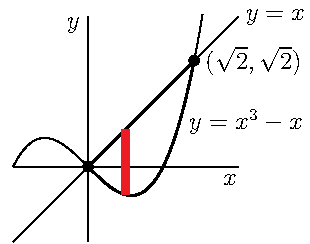
\includegraphics{OE02A_2a}
\end{center}
The top and bottom boundaries of the specified region are $y=T(x)=x$
and $y=B(x)=x^3-x$, respectively. So,
\begin{align*}
{\rm Area} = \int_0^{\sqrt{2}}\big[T(x)-B(x)\big]\ \dee{x}
= \int_0^{\sqrt{2}}\big[x-(x^3-x)\big]\ \dee{x} = \int_0^{\sqrt{2}} 2x-x^3 \ \dee{x}
\end{align*}

\end{solution}
%%%%%%%%%%%%%%%%%%%%%%%%%%%%%%%%%%%%%%%%


\begin{question}[2000D]
Write down a definite integral that represents the
area of the region bounded by the line $y=-\dfrac{x}{2}$
and the parabola $y^2=6-\dfrac{5x}{4}$.
\emph{Do not evaluate the integral explicitly.}
\end{question}


\begin{hint}
Draw a sketch first.
\end{hint}

\begin{answer}
$\displaystyle \int_{-3/2}^{4}\left[\frac{4}{5}(6-y^2)+2y\right]\ \dee{y}$
\end{answer}

\begin{solution}
We need to find where the curves intersect.
\begin{align*}
\frac{x^2}{4}=y^2&=6-\dfrac{5x}{4}\\
\frac{1}{4}x^2+\frac{5}{4}x-6&=0\\
x^2+5x-24&=0\\
(x+8)(x-3)&=0\\
x=-8,\quad x&=3
\end{align*}

The curves intersect at $(-8,4)$ and $(3,-\frac{3}{2})$.  Using horizontal
strips:
\begin{center}
       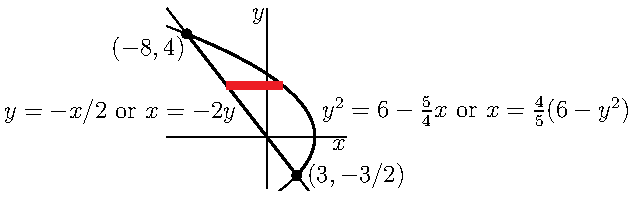
\includegraphics{OE00D_3a}
\end{center}
we have
\begin{align*}
\text{Area} = \int_{-3/2}^{4}\Big[\frac{4}{5}(6-y^2)+2y\Big]\ \dee{y}
\end{align*}

\end{solution}
%%%%%%%%%%%%%%%%%%%%%%%%%%%%%%%%%%%%%%%%


\begin{question}[2001A]\label{1.5_4ax4ay}
Write down a definite integral that represents the
area of the finite plane region bounded by $y^2=4ax$ and
$x^2=4ay$, where $a>0$ is a constant.
\emph{Do not evaluate the integral explicitly.}
\end{question}

\begin{hint}
You can probably find the intersections by inspection.
\end{hint}

\begin{answer}
$ \displaystyle\int_0^{4a}\left[\sqrt{4ax}-\frac{x^2}{4a}\right]\ \dee{x}$
\end{answer}

\begin{solution}
If the curves intersect at $(x,y)$, then
\begin{align*}
\left(x^2\right)^2&=\left(4a\right)^2y^2 = (4a)^24ax\\
x^4&=(4a)^3 x\\
x^4&-(4a)^3x=0\\
x(&x^3-(4a)^3)=0\\
x&= 0 \quad\mbox{or}\quad x^3=(4a)^3
\end{align*}
The curves intersect at $(0,0)$ and $(4a,4a)$. (It is also possible to find these points by inspection.) Using vertical strips:
\begin{center}
       
\includegraphics{OE01A_2a}
\end{center}
We want the $y$-values of the functions. We write the top  function as $y =\sqrt{4ax}$ (we care about the positive square root, not the negative one) and we write the bottom function as $y=\frac{x^2}{4a}$.
Then we have
\begin{align*}
\text{Area} = \int_0^{4a}\left[\sqrt{4ax}-\frac{x^2}{4a}\right]\ \dee{x}
\end{align*}

\end{solution}
%%%%%%%%%%%%%%%%%%%%%%%%%%%%%%%%%%%%%%%%

\begin{Mquestion}[2001D]
Write down a definite integral that represents the
area of the region bounded between the line $x+12y+5=0$
and the curve  $x=4y^2$.
\emph{Do not evaluate the integral explicitly.}
\end{Mquestion}

\begin{hint}
To find the intersection, plug $x=4y^2$ into the equation $x+12y+5=0$.
\end{hint}

\begin{answer}
$\displaystyle\int_1^{25}\left[-\frac{1}{12}(x+5)+\frac{1}{2}\sqrt{x}\right]\ \dee{x}$
\end{answer}

\begin{solution}
The curves intersect when $x=4y^2$ and $0=4y^2+12y+5
=(2y+5)(2y+1)$. So, the curves intersect at $(1,-\half)$ and $(25,-\frac{5}{2})$.
Using vertical strips:
\begin{center}
       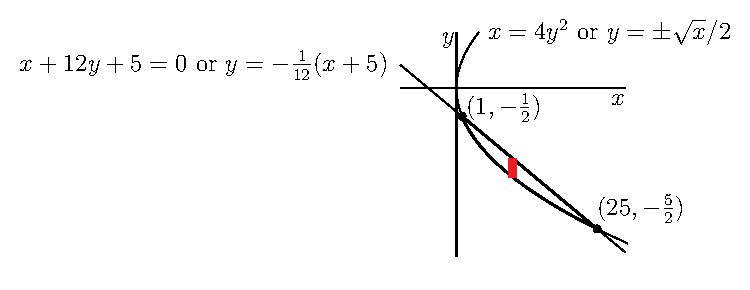
\includegraphics{OE01D_3a}
\end{center}
we have
\begin{align*}
\text{Area} =
\int_1^{25}\left[-\frac{1}{12}(x+5)+\frac{1}{2}\sqrt{x}\right]\ \dee{x}
\end{align*}

\end{solution}
%%%%%%%%%%%%%%%%%%%%%%%%%%%%%%%%%%%%%%%%



%%%%%%%%%%%%%%%%%%
\subsection*{\Procedural}
%%%%%%%%%%%%%%%%%%



\begin{Mquestion}[M105 2013A]
Find the area of the region bounded by the graph of
$f (x) = \dfrac{1}{(2x-4)^2}$ and the $x$--axis
between $x = 0$ and $x = 1$.
\end{Mquestion}

\begin{hint}
If the bottom function is the $x$-axis, this is a familiar question.
\end{hint}

\begin{answer}
$\dfrac{1}{8}$
\end{answer}

\begin{solution}
\begin{center}
\begin{tikzpicture}
\YEaaxis{1}{3.5}{1}{2}
\YExcoord{2}{1}
\draw[thick] plot[domain=-.5:1.5, samples=50, scale=2](\x,{1/(4*(\x-2)*(\x-2))});
\draw[fill=blue, fill opacity=0.5] plot[domain=0:1, samples=10, scale=2](\x,{1/(4*(\x-2)*(\x-2))})--(2,0)-|cycle;
\draw (3,1.5)node[right]{$y=\frac{1}{(2x-4)^2}$};
\end{tikzpicture}
\end{center}

The area between the curve $y= \frac{1}{(2x-4)^2}$
and the $x$-axis, with $x$ running from $a=0$ to
$b=1$, is exactly the definite integral of $\frac{1}{(2x+4)^2}$ with limits $0$ and $1$.

\begin{align*}
\mbox{Area}&=\int_0^1 \frac{\dee{x}}{(2x-4)^2}&u=2x-4,\quad\dee{u}=2\ \dee{x}\\
&=\frac{1}{2}\int_{-4}^{-2}\frac{1}{u^2}\dee{u} = \frac{1}{2}\left[\frac{-1}{u}\right]_{u=-4}^{u=-2}\\
&=\frac{1}{2}\Big[\frac{1}{2}-\frac{1}{4}\Big]
=\frac{1}{8}
\end{align*}

\end{solution}
%%%%%%%%%%%%%%%%%%%

\begin{question}[2016Q2]
Find the area between the curves $y=x$ and $y=3x-x^2$, by first identifying the points of intersection and then integrating.
\end{question}

\begin{hint}
Part of the job is to determine whether $y=x$ lies above or below
$y=3x-x^2$.
\end{hint}

\begin{answer}
$\dfrac{4}{3}$
\end{answer}

\begin{solution}
If the curves $y=f(x)=x$ and $y=g(x)=3x-x^2$ intersect at $(x,y)$, then
\begin{align*}
3x-x^2&=y=x\\
x^2-2x&=0\\
x(x-2)&=0\\
x=0 \quad &\mbox{or} \quad x=2
\end{align*}
Furthermore, $g(x)-f(x) = 2x-x^2 = x(2-x)$ is positive for all $0\le x\le 2$.
That is, the curve  $y=3x-x^2$ lies above the line $y=x$ for all $0\le x\le 2$.

\begin{center}
\begin{tikzpicture}
\YEaaxis{1}{5}{1}{3}
\draw[thick, blue] plot[domain=-.2:3.25, scale=1.5, samples=40](\x,{3*\x-\x*\x});
\draw[thick] (-.75,-.75)--(3.5,3.5) node[right]{$y=x$};
\draw[blue] (4.5,1) node[right]{$y=3x-x^2$};
\YExcoord{3}{2}
\end{tikzpicture}
\end{center}

We therefore evaluate the integral:
\begin{align*}
 \int_0^2 \big[ (3x-x^2) - x \big] \,\dee{x}
  = \int_0^2 [2x-x^2]\,\dee{x}
   = \bigg[x^2 - \frac{x^3}{3}\bigg]^{2}_{0}
   = \bigg[ 4-\frac{8}{3} \bigg] -0
   = \frac{4}{3}
\end{align*}
\end{solution}
%%%%%%%%%%%%%%%%%%%



\begin{question}[2015A]
Calculate the area of the region enclosed by $y = 2^x$ and $y = \sqrt x+1$.
\end{question}

\begin{hint}
Guess the intersection points by trying small integers.
\end{hint}

\begin{answer}
$\dfrac{5}{3}-\dfrac{1}{\log 2}$
\end{answer}

\begin{solution}
By inspection, the two curves cross at $(0,1)$ and $(1,2)$.


\begin{center}
\begin{tikzpicture}
\YEaaxis{1}{3}{1}{3}
\draw[thick, blue] plot[domain=0:2, xscale=2, yscale=1.5, samples=140](\x,{sqrt(\x)+1});
\draw[thick] plot[domain=-.5:1.5, xscale=2,yscale=1.5,  samples=40](\x,{pow(2,\x)});
\draw[blue] (4,3) node[right]{$y=\sqrt{x}+1$};
\draw (-1,1) node[left]{$y=2^x$};
\YExcoord{2}{1}
\end{tikzpicture}
\end{center}


To antidifferentiate $2^x$, we write $2^x={(e^{\log 2})}^x=e^{x\log 2}$.
\begin{align*}
\text{Area} &= \int_0^1\big[(\sqrt{x}+1)-e^{x\log 2}\big]\,\dee{x}
=\left[\frac{2}{3}x^{3/2}+x-\frac{1}{\log 2} 2^x\right]_0^1 \\
&=\frac{2}{3}+1-\frac{1}{\log 2}[2-1]
=\frac{5}{3}-\frac{1}{\log 2}
\end{align*}
\end{solution}
%%%%%%%%%%%%%%%%%%%


\begin{question}[2014A]
Find the area of the finite region bounded between the two curves
$y = \sqrt{2} \cos(\pi x/4)$ and $y = |x|$.
\end{question}

\begin{hint}
Draw a sketch first. You can also exploit a symmetry of the region
to simplify your solution.
\end{hint}

\begin{answer}
$\dfrac{8}{\pi}-1$
\end{answer}

\begin{solution}
Here is a sketch of the specified region.

\begin{center}
       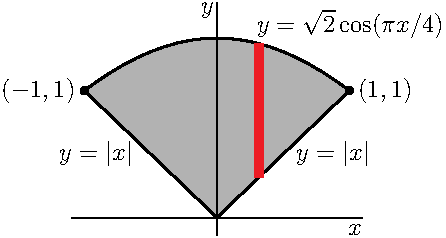
\includegraphics{OE14A_2}
\end{center}

\noindent
Both functions are even, so the region  is symmetric about the $y$--axis.
So, we will compute the area of the part with $x\ge 0$ and multiply
by $2$. The curves $y=\sqrt{2} \cos(\pi x/4)$ and $y=x$ intersect
when $x=\sqrt{2} \cos(\pi x/4)$ or $\cos(\pi x/4)=\frac{x}{\sqrt{2}}$,
which is the case\footnote{The solution $x=1$ was found by guessing.
To guess a solution to $\cos(\pi x/4)=\frac{x}{\sqrt{2}}$ just ask
yourself what simple angle has a cosine that involves $\sqrt{2}$. This
guessing strategy is essentially useless in the real world, but
works great on problem sets and exams.}
when $x=1$. So, using vertical strips as in
the figure above, the area (including the multiplication by 2) is
\begin{equation*}
2\int_0^1 \big[\sqrt{2} \cos(\pi x/4) - x\big]\,\dee{x}
= 2\bigg[\sqrt{2}\,\frac{4}{\pi} \sin(\pi x/4)-\frac{x^2}{2}\bigg]_0^1
= 2\bigg[\frac{4}{\pi}-\frac{1}{2}\bigg] = \frac{8}{\pi}-1
\end{equation*}

\end{solution}
%%%%%%%%%%%%%%%%%%%

\begin{Mquestion}[2016Q2]
Find the area of the finite region that is bounded by the graphs of
$f(x) = x^2\sqrt{x^3+1}$ and $g(x) = 3x^2$.
\end{Mquestion}

\begin{hint}
Figure out where the two curves cross. To determine which curve is above the
other, try evaluating $f(x)$ and $g(x)$ for some simple value of $x$.
Alternatively, consider $x$ very close to zero.
\end{hint}

\begin{answer}
$\dfrac{20}{9}$
\end{answer}

\begin{solution}
For our computation, we will need an antiderivative of
$x^2\sqrt{x^3+1}$, which can be found using the substitution
$u=x^3+1$, $\dee{u} = 3x^2\,\dee{x}$:
\begin{align*}
\int x^2\sqrt{x^3+1} \, \dee{x} = \int \sqrt u \cdot \frac13\,\dee{u} = \frac13\int u^{1/2}\,\dee{u} = \frac13\cdot \frac{u^{3/2}}{3/2}+C = \frac29(x^3+1)^{3/2} + C.
\end{align*}

The two functions $f(x)$ and $g(x)$ are clearly equal at $x=0$. If $x\ne0$, then the functions are equal when
\begin{align*}
3x^2 &= x^2\sqrt{x^3+1} \\
3 &= \sqrt{x^3+1} \\
9 &= x^3+1 \\
8 &= x^3 \\
2 &= x.
\end{align*}
The function $g(x)=3x^2$ is the larger of the two on the interval $[0,2]$, as can be seen by plugging in $x=1$, say, or by observing that when $x$
is very small $f(x)=x^2\sqrt{x^3+1}\approx x^2$ and $g(x)=3x^2$.

\begin{center}
%\begin{tikzpicture}
%\draw[dashed] (4,-0.2) -- (4,6) -- (-0.2,6);
%\draw[domain=0:2.1] plot (2*\x,{\x*\x*sqrt(\x*\x*\x+1)/2});
%\draw[domain=0:2.2] plot (2*\x,{3*\x*\x/2});
%\node[below] at (4,-0.2) {$2$};
%\node[left] at (-0.2,6) {$12$};
%\node at (2,3) {$y=3x^2$};
%\node at (3,0.4) {$y=x^2\sqrt{x^3+1}$};
%\draw[ultra thick,->] (0,0) -- (5,0);
%\draw[ultra thick,->] (0,0) -- (0,8);
%\end{tikzpicture}
     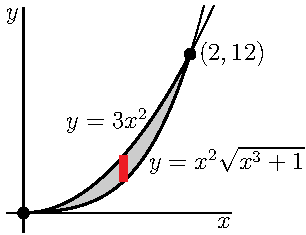
\includegraphics{OQ16_2_4}
\end{center}

The area in question is therefore:
\begin{align*}
\int_0^2 \big( 3x^2 - x^2\sqrt{x^3+1} \big) \, \dee{x} &= \bigg( {x^3} - \frac29(x^3+1)^{3/2} \bigg) \bigg|_0^2 \\
&= \bigg( 2^3 - \frac2 9(2^3+1)^{3/2} \bigg) - \bigg( 0^3 - \frac29(0^3+1)^{3/2} \bigg) \\
&= \bigg( 8 - 6 \bigg) - \bigg( 0 - \frac 2 9 \bigg) =\frac{20}9.
\end{align*}
\end{solution}
%%%%%%%%%%%%%%%%%%%

\begin{Mquestion}[2016Q2]
Find the area to the left of the $y$--axis and to
the right of the curve $x=y^2+y$.
\end{Mquestion}

\begin{hint}
Think about whether it will easier to use vertical strips or horizontal strips.
\end{hint}

\begin{answer}
$\dfrac{1}{6}$
\end{answer}

\begin{solution}
First, let's figure out what our curve $x=y^2+y=y(y+1)$ looks like.
\begin{itemize}
\item The curve intercepts the $y$-axis when $y=0$ and $y=-1$.
\item The $x$-values of the curve are negative when $-1<y<0$, and  positive elsewhere.
\end{itemize}
 This leads to the figure below. We're evaluating the area from $y=-1$ to $y=0$. Since $y^2+y$ is negative there, the length of our (horizontal) slices are $0-(y^2+y)$.

\vspace{0.4in}
\begin{align*}
\text{Area}=\int_{-1}^0\big(0-(y^2+y)\big)\,\dee{y} = -\bigg[\frac{y^3}{3}+\frac{y^2}{2}\bigg]_{-1}^0
=-\frac13+\frac12
=\frac{1}{6}\quad
\smash{\raisebox{-0.33\height}{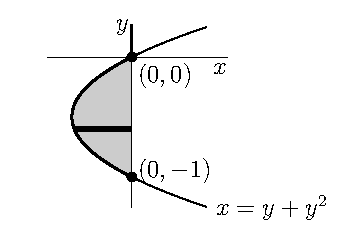
\includegraphics{quiz2M1prob2}}}
\end{align*}
\vspace{0.2in}

\end{solution}
%%%%%%%%%%%%%%%%%%%

\begin{question}
Find the area of the finite region  below $y=\sqrt{9-x^2}$ and above both
 $y=|x|$ and $y=\sqrt{1-x^2}$.
\end{question}
\begin{hint}
Writing an integral for this is nasty. How can you avoid it?
\end{hint}
\begin{answer}
$2\pi$
\end{answer}
\begin{solution}
Let's begin by sketching our region. Note that $y=\sqrt{1-x^2}$ and $y=\sqrt{9-x^2}$ are the top halves of circles centred at the origin with radii 1 and 3, respectively.
\begin{center}
\begin{tikzpicture}
\YEaaxis{4}{4}{1}{4}
\draw[thick] (-3,3)--(0,0)--(3,3);
\draw[thick] (-1,0) arc(180:0:1cm);
\draw[thick] (-3,0) arc(180:0:3cm);
\draw[fill=blue, fill opacity=0.5] (-.71,.71)--(-2.12,2.12) arc(135:45:3) --(.71,.71) arc(45:135:1cm);
\draw (3,.5) node[right] {$y=\sqrt{9-x^2}$};
\draw (3,3) node[right] {$y=|x|$};
\end{tikzpicture}
\end{center}
Our region is the difference of two quarter-circles, so we find its area using geometry:
\[\mbox{Area}=\frac{1}{4}\left(\pi\cdot 3^2\right)-\frac{1}{4}\left(\pi\cdot 1^2\right)=2\pi\]
\end{solution}

%%%%%%%%%%%%%%%%%%%








%%%%%%%%%%%%%%%%%%
\subsection*{\Application}
%%%%%%%%%%%%%%%%%%%

\begin{Mquestion}[2013A]\label{prob_s1.5q5}
The graph below shows the region between
$y = 4 + \pi \sin x$ and $y = 4 + 2\pi - 2x$.

\begin{center}
       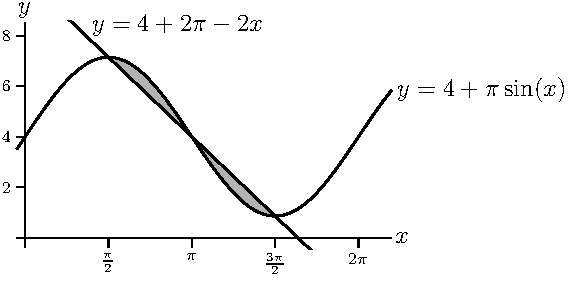
\includegraphics{OE13A_4a}
\end{center}

\noindent Find the area of this region.
\end{Mquestion}

\begin{hint}
You are asked for the area, not the signed area. Be very careful about signs.
\end{hint}

\begin{answer}
$2\Big[\pi-\frac{1}{4}\pi^2\Big]$
\end{answer}

\begin{solution}
We will compute the area by using thin vertical strips, as in
the sketch  below:

\begin{center}
       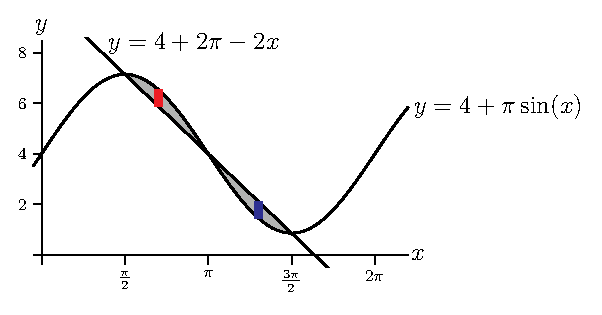
\includegraphics{OE13A_4}
\end{center}

\noindent
By looking at the sketch above, we guess the line $y = 4 + 2\pi - 2x$ intersects the curve
$y = 4 + \pi \sin x$ when $x=\frac{\pi}{2},$ $x=\pi$, and $x=\frac{3\pi}{2}$. Let's make sure these are correct by plugging them into the two equations, and making sure the $y$-values match:

\begin{center}
\begin{tabular}{|c|c|c|c|}
\hline
$x$ & $4+2\pi-2x$ & $4+\pi\sin(x)$ & match?\\[5pt]
\hline
$\frac{\pi}{2}$ & $4+\pi$ & $4+\pi $ & \checkmark\\[5pt]
\hline
$\pi$ & $4$ & $4$ & \checkmark\\[5pt]
\hline
$\frac{3\pi}{2}$ & $4-\pi$ & $4-\pi $ & \checkmark\\[5pt]
\hline
\end{tabular}
\end{center}
Also from
the sketch, we see that:
\begin{itemize}
\item
When $\frac{\pi}{2} \le x \le \pi$, the top of the strip is at
$y = 4 + \pi \sin x$ and the bottom of the strip is at $y = 4 + 2\pi - 2x$.
So the strip has height $\big[(4 + \pi \sin x)-(4 + 2\pi - 2x)\big]$
and width $\dee{x}$, and hence area
$\big[(4 + \pi \sin x)-(4 + 2\pi - 2x)\big]\dee{x}$.

\item
When $\pi \le x \le \frac{3\pi}{2}$, the top of the strip is at
$y = 4 + 2\pi - 2x$ and the bottom of the strip is at $y = 4 + \pi \sin x$.
So the strip has height $\big[(4 + 2\pi - 2x)-(4 + \pi \sin x)\big]$
and width $\dee{x}$, and hence area
$\big[(4 + 2\pi - 2x)-(4 + \pi \sin x)\big]\dee{x}$.
\end{itemize}
Now we can calculate:
\begin{align*}
\hbox{Area}
&= \int_{\pi/2}^\pi \big[(4 + \pi \sin x)-(4 + 2\pi - 2x)\big]\ \dee{x}
   +\int^{3\pi/2}_\pi \big[(4 + 2\pi - 2x)-(4 + \pi \sin x)\big]\ \dee{x}\\
&= \int_{\pi/2}^\pi \big[\pi \sin x- 2\pi + 2x\big]\ \dee{x}
   +\int^{3\pi/2}_\pi \big[2\pi - 2x- \pi \sin x\big]\ \dee{x}\\
&=\Big[-\pi \cos x- 2\pi x + x^2\Big]_{\pi/2}^\pi
  +\Big[2\pi x - x^2+ \pi \cos x\Big]^{3\pi/2}_\pi\\
&=\left[\pi-\pi^2+\frac{3}{4}\pi^2\right]
  +\left[\pi^2-\frac{5}{4}\pi^2+\pi\right]\\
&=2\Big[\pi-\frac{1}{4}\pi^2\Big]
\end{align*}
\end{solution}
%%%%%%%%%%%%%%%%%%%


\begin{question}[1998A]
Compute the area of the finite region bounded by the
curves $x=0$, $x=3$, $y=x+2$ and $y=x^2$.
\end{question}

\begin{hint}
You are asked for the area, not the signed area. Draw a sketch of the region
and be very careful about signs.
\end{hint}

\begin{answer}
$\dfrac{31}{6}$
\end{answer}

\begin{solution}
First, here is a sketch of the region. We are not asked for it, but it
is crucial for understanding the question.
\begin{center}
       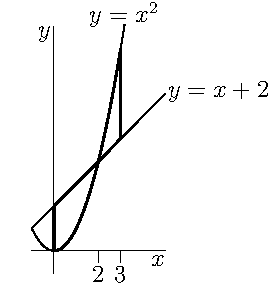
\includegraphics{graphE98A_3}
\end{center}
The two curves  $y=x+2$ and $y=x^2$ cross at $(2,4)$.
The area of the part between them with $0\le x\le 2$ is:
\begin{align*}
\int_0^2 \big[x+2-x^2\big]\,\dee{x}=\Big[\frac{1}{2} x^2+2x-\frac{1}{3}x^3\Big]_0^2
=2+4-\frac{8}{3}=\frac{10}{3}
\end{align*}
The area of the part between the two curves with $2\le x\le 3$ is:
\begin{align*}
\int_2^3 \big[x^2-(x+2)\big]\,\dee{x}=\Big[\frac{1}{3}x^3-\frac{1}{2} x^2-2x\Big]_2^3
=9-\frac{9}{2}-6-\frac{8}{3}+2+4=\frac{11}{6}
\end{align*}
The total area is $\dfrac{10}{3}+\dfrac{11}{6}=\dfrac{31}{6}$.

\end{solution}
%%%%%%%%%%%%%%%%%%%

\begin{question}[2016Q2]
Find the total area between the curves $y = x \sqrt{25-x^2}$ and $y=3x$, on the interval $0\le x\le 4$.
\end{question}

\begin{hint}
You have to determine whether
\begin{itemize}
\item
   the curve $y = f(x) = x \sqrt{25-x^2}$ lies above the line $y=g(x)=3x$ for all          $0\le x\le 4$ or
\item
the curve $y = f(x)$ lies below the line $y=g(x)$ for all $0\le x\le 4$ or
\item  $y=f(x)$ and $y=g(x)$ cross somewhere between $x=0$ and $x=4$.
\end{itemize}
One way to do so is to study the sign of
      $f(x)-g(x) = x\big(\sqrt{25-x^2}-3\big)$.
\end{hint}

\begin{answer}
$\dfrac{26}{3}$
\end{answer}

\begin{solution}
We need to figure out which curve is on top, when. To do this, set $h(x) = 3x - x\sqrt{25-x^2}$. If $h(x) > 0$, then $y=3x$ is the top curve; if $h(x)<0$, then $y=x\sqrt{25-x^2}$ is the top curve.
\begin{align*}
h(x) &= 3x - x\sqrt{25-x^2} = x\left[3-\sqrt{25-x^2}\right]
\intertext{We only care about values of $x$ in $[0,4]$, so $x$ is nonnegative. Then $h(x)$ is positive when:}
3&> \sqrt{25-x^2}\\
9&> 25-x^2\\
x^2 & > 16\\
x&> 4
\end{align*}


That is, $h(x)$ is never positive over the interval $[0,4]$. So, $y = x \sqrt{25-x^2}$ lies above $y=3x$ for all $0\le x\le 4$.

The area we need to calculate is therefore:
\begin{align*}
A &= \int_0^4 \left[x \sqrt{25-x^2} - 3x\right]\,\dee{x} \\
&= \int_0^4 x \sqrt{25-x^2}\,\dee{x} - \int_0^4 3x\,\dee{x} \\&= A_1 - A_2.
\end{align*}
To evaluate $A_1$, we use the substitution
$u(x) = 25-x^2$, for which $\dee{u} = u'(x)\,\dee{x}= -2x\,\dee{x}$;
and $u(4)=25-4^2=9$ when $x=4$,
while $u(0)=25-0^2=25$ when $x=0$. Therefore
\begin{align*}
A_1 &= \int_{x=0}^{x=4} x \sqrt{25-x^2}\,\dee{x}
= -\frac{1}{2} \int_{u=25}^{u=9} \sqrt{u}\,\dee{u}
= \left[-\frac{1}{3} u^{3/2} \right]_{25}^{9}
= \frac{125 - 27}{3} = \frac{98}{3}
\end{align*}
For $A_2$ we use the antiderivative directly:
\begin{equation*}
A_2 = \int_0^4 3x\,\dee{x} =\left[ \frac{3x^2}{2} \right]_0^4 = 24
\end{equation*}
Therefore the total area is:
\begin{align*}
A = \frac{98}{3} - 24 = \frac{26}{3}
\end{align*}

\end{solution}
%%%%%%%%%%%%%%%%%%%

%%%%%%%%%%%%%%%%%%


\begin{question}
Find the area of the finite region below $y=\sqrt{9-x^2}$ and $y=x$, and above  $y=\sqrt{1-(x-1)^2}$.
\end{question}
\begin{hint}
Flex those geometry muscles.
\end{hint}
\begin{answer}
$\dfrac{7\pi}{8}-\dfrac{1}{2}$
\end{answer}
\begin{solution}
Let's begin by sketching our region. Note that $y=\sqrt{9-x^2}$ is the top half of a circle centred at the origin with radius 3, while $y=\sqrt{1-(x-1)^2}$ is the top half of a circle of radius 1 centred at $(1,0)$.
\begin{center}
\begin{tikzpicture}
\YEaaxis{4}{4}{1}{4}
\draw[thick] (-1,-1)--(0,0)--(3,3);
\draw[thick] (0,0) arc(180:0:1cm);
\draw[thick] (-3,0) arc(180:0:3cm);
\draw[fill=blue, fill opacity=0.5] (2.12,2.12) arc(45:0:3cm)--(2,0) arc(0:90:1) --cycle ;
\end{tikzpicture}
\end{center}

Note $y=x$ intersects $y=\sqrt{1-(x-1)^2}$ at $(1,1)$, the highest part of the smaller half-circle.

We can easily take the area of  triangles and sectors of circles. With that in mind, we cut up our region the following way:

\begin{center}
\begin{tikzpicture}
\YEaaxis{4}{4}{1}{4}
\draw[thick] (-1,-1)--(0,0)--(3,3);
\draw[thick] (0,0) arc(180:0:1cm);
\draw[thick] (-3,0) arc(180:0:3cm);
\draw[thick, dashed, red, fill=red, fill opacity=0.5] (0,0)--(1,1)|-cycle;
\draw[red] (.5,-.25) node{$A_1$};
\draw[thick, dashed, green, fill=green, fill opacity=0.5] (1,0) --(1,1)arc(90:0:1cm)--cycle;
\draw[green] (1.5,-.25) node{$A_2$};
\draw[blue, ultra thick, fill opacity=0.5, pattern=crosshatch, pattern color=blue] (0,0)--(2.12,2.12) arc(45:0:3cm)--cycle;
\draw[blue] (3.5,1) node{$A_3$};
\end{tikzpicture}
\end{center}
\begin{itemize}
\item The desired area is $A_3-(A_1+A_2)$.
\item $A_1$ is the area of right a triangle with base 1 and height 1, so $A_1 = \frac{1}{2}$.
\item $A_2$ is the area of a quarter circle of radius 1, so $A_2=\frac{\pi}{4}$.
\item $A_3$ is the area of an eighth of a circle of radius 3, so $A_2 = \frac{9\pi}{8}$
\end{itemize}
So, the area of our region is~~ $\dfrac{9\pi}{8} - \dfrac{1}{2}-\dfrac{\pi}{4}=\dfrac{7\pi}{8}-\dfrac{1}{2}$.
\end{solution}

%%%%%%%%%%%%%%%%%%%


\begin{Mquestion}
Find the area of the finite region bounded by the curve $y=x(x^2-4)$ and the line $y=x-2$.
\end{Mquestion}
\begin{hint}
These two functions have three points of intersection. This question is slightly messy, but uses the same concepts we've been practicing so far.
\end{hint}
\begin{answer}
$12\sqrt{2}-\dfrac{13}{4}$
\end{answer}
\begin{solution}
The first function is a cubic, with intercepts at $x=0,\pm2$. The second is a straight line  with a positive slope.

We need to figure out what these functions look like in relation to one another, so let's find their points of intersection.
\begin{align*}
x(x^2-4)&=x-2\\
x(x+2)(x-2)&=x-2\\
\boxed{\color{blue}x-2=0} \quad\mbox{or}\quad x(x+2)&=1\\
x^2+2x-1&=0\\
x &= \dfrac{-2\pm\sqrt{4-4(1)(-1)}}{2}\\
x&=\boxed{\color{red}-1\pm \sqrt{2}}
\end{align*}
So, our three points of intersection are when {\color{blue}$x=2$} and when ${\color{red}x=-1\pm\sqrt{2}}$. We note \[\textcolor{red}{-1-\sqrt{2}} <\textcolor{red}{ -1+\sqrt{2} }< -1+\sqrt{4}<\textcolor{blue}{2}\ .\] So, we need to see which function is on top over the two intervals $\left[-1-\sqrt{2},-1+\sqrt{2}\right]$ and $\left[-1+\sqrt{2},2\right]$. It suffices to check points in these intervals.

\begin{center}
\begin{tabular}{|c|c|c|c|}
\hline
$x$&$x(x^2-4)$ & $x-2$ & top function:\\
\hline
0 & 0 & $-2$ & $x(x^2-4)$\\
\hline
1 & -3 & $-1$ & $x-2$\\
\hline
\end{tabular}
\end{center}


Since 0 is in the interval $\left[-1-\sqrt{2},-1+\sqrt{2}\right]$, $x(x^2-4)$ is the top function in that interval.
Since 1 is in the interval $\left[-1+\sqrt{2},2\right]$, $x-2$ is the top function in that interval. Now we can set up the integral to evaluate the area:
\begin{alignat*}{3}
\mbox{Area}&=\int_{-1-\sqrt{2}}^{-1+\sqrt{2}}\left[x(x^2-4) - (x-2)\right]\ \dee{x}  \quad&&+ \quad
&&\int_{-1+\sqrt{2}}^{2}\left[(x-2)-x(x^2-4)\right]\ \dee{x}\\
&=\int_{-1-\sqrt{2}}^{-1+\sqrt{2}}\left[x^3-5x+2\right]\ \dee{x}  \quad&&+ \quad
&&\int_{-1+\sqrt{2}}^{2}\left[-x^3+5x-2\right]\ \dee{x}
\\&=\left[\frac{1}{4}x^4 - \frac{5}{2}x^2+2x\right]_{-1-\sqrt{2}}^{-1+\sqrt{2}}  \quad&&+ \quad
&&\left[-\frac{1}{4}x^4 + \frac{5}{2}x^2-2x\right]_{-1+\sqrt{2}}^{2}
\intertext{After some taxing but rudimentary algebra:}
&=\left(8\sqrt{2}\right)+\left(4\sqrt{2}-\frac{13}{4}\right)=12\sqrt{2}-\frac{13}{4}
\end{alignat*}
\end{solution}
%%%%%%%%%%%%%%%%%%%

\section{Volumes}
%
% Copyright 2018 Joel Feldman, Andrew Rechnitzer and Elyse Yeager.
% This work is licensed under a Creative Commons Attribution-NonCommercial-ShareAlike 4.0 International License.
% https://creativecommons.org/licenses/by-nc-sa/4.0/
%
\questionheader{ex:s1.6}

%%%%%%%%%%%%%%%%%%
\subsection*{\Conceptual}
%%%%%%%%%%%%%%%%%%
\begin{question}
Consider a right circular cone.
\begin{center}
\begin{tikzpicture}
\draw (0,0)node[thin, gray, shape=ellipse, minimum width=3cm, minimum height=1cm, draw, fill=black, fill opacity=0.1] {};
\draw (-1.5,0)--(0,3)--(1.5,0);
\filldraw[draw=blue, left color=blue!50!black, right color=white, opacity=0.3] (-1.5,0)--(0,3)--(1.5,0) arc(0:-180:1.5cm and 0.5cm);

\end{tikzpicture}
\end{center}
What shape are horizontal cross-sections? Are the vertical cross-sections the same?
\end{question}
\begin{hint}
The horizontal cross-sections were discussed in Example~\eref{CLP101}{eg:VOLa} of
the CLP-2 text.
\end{hint}
\begin{answer}
The horizontal cross-sections are circles, but the vertical cross-sections are not.
\end{answer}
\begin{solution}
If we take a horizontal slice of a cone, we get a circle. If we take a vertical cross-section, the base is flat (it's a chord on the circular base of the cone), so we know right away it isn't a circle. Indeed, if we slice down through the very centre, we get a triangle. (Other vertical slices have a curvy top, corresponding to  a class of curves known as hyperbolas.)
\end{solution}

\begin{Mquestion}
Two potters start with a block of clay $h$ units tall, and identical square cookie cutters. They form columns by pushing the square cookie cutter straight down over the clay, so that its cross-section is the same square as the cookie cutter. Potter A pushes their cookie cutter down while their clay block is sitting motionless on a table; Potter B pushes their cookie cutter down while their clay block is rotating on a potter's wheel, so their column looks twisted. Which column has greater volume?

\begin{center}
\hfill
\begin{tikzpicture}
\draw[thick] (-1.5,-3) --(-0,-3.5)--(1.5,-3)--(1.5,3)--(0,2.5)--(-1.5,3)--cycle;
\draw[thick] (-1.5,3)--(0,3.5)--(1.5,3) (0,2.5)--(0,-3.5);
\fill[bottom color=black, top color=white, fill opacity=0.2] (-1.5,3)--(0,2.5)--(0,-3.5)--(-1.5,-3)--cycle;
\fill[bottom color=blue, top color=white, fill opacity=0.2] (1.5,3)--(0,2.5)--(0,-3.5)--(1.5,-3)--cycle;
 \draw (0,-4.5) node {Column A};
\end{tikzpicture}
\hfill
\begin{tikzpicture}
\draw[thick] (-1.5,-3)--(0,-3.5)--(1.5,-3);
\draw[thick] plot[domain=-1.57:1.57]({-1.5*sin(\x r)},1.91*\x);
\draw[thick] (-1.5,3)--(0,2.5)--(1.5,3)--(0,3.5)--cycle;
\draw[thick] plot[domain=-2.1:0, yshift=2.5cm]({-1.25*sin(\x r)},1.91*\x);
\draw[thick] plot[domain=.6:1.57]({1.5*sin(\x r)},1.91*\x);
\draw[thick] plot[domain=-1.57:-.8]({1.5*sin(\x r)},1.91*\x);
\draw[thick] plot[domain=-.75:1.57, yshift=-.5cm]({-1.25*cos(\x r)},-1.91*\x);
\fill[bottom color=black, top color=white, fill opacity=0.5] (0,-3.5)-- plot[domain=-.8:-1.57]({1.5*sin(\x r)},1.91*\x)  plot[domain= .6:1.57, yshift=-.5cm]({-1.25*cos(\x r)},-1.91*\x);
\fill[bottom color=red, top color=white, fill opacity=0.2] (0,2.5) plot[domain=-2.1:0, yshift=2.5cm]({-1.25*sin(\x r)},1.91*\x)--
plot[domain=1.57:-.8]({-1.5*sin(\x r)},1.91*\x)--cycle;
\fill[bottom color=blue, top color=white, fill opacity=0.2] (0,-3.5) --(1.5,-3)
 plot[domain=-1.57:.6]({-1.5*sin(\x r)},1.91*\x)--
plot[domain=-.75:1.57, yshift=-.5cm]({-1.25*cos(\x r)},-1.91*\x);
\fill[bottom color=green!50!blue, top color=white, fill opacity=0.2] (0,2.5) --(1.5,3)
 plot[domain=.6:1.57]({1.5*sin(\x r)},1.91*\x)--(0,2.5)--
 cycle;
 \draw (0,-4.5) node {Column B};
\end{tikzpicture}
\hfill~
\end{center}
\end{Mquestion}
\begin{hint}
What are the dimensions of the cross-sections?
\end{hint}
\begin{answer}
The columns have the same volume.
\end{answer}
\begin{solution}
The columns have the same volume. We can see this by chopping up the columns into horizontal cross-sections. Each cross-section has the same area as the cookie cutter, $A$, and height $\dee{y}$. Then in both cases, the volume of the column is
\[\int_{0}^h A~\dee{y}  = hA \mbox{ cubic units}\]
\end{solution}

%%%%%%%%%%%%%%%%%%
\begin{question}
Let $R$ be the region bounded above by the graph of $y=f(x)$ shown below and bounded below by the $x$-axis, from $x=0$ to $x=6$. Sketch the washers that are formed by rotating $R$ about the $y$-axis.
In your sketch, label the all radii in terms of $y$, and label the thickness.
\begin{center}
\begin{tikzpicture}
\YEaaxis{1}{7}{1}{4}
\draw[ultra thick, blue] (0,0)--(1,1)--(2,0)--(4,3)--(6,0);
\draw[blue](6,1) node  [right]{$y=f(x)$};
\foreach \x in {2,1,4,6}{\YExcoord{\x}{\x}}
\foreach \x in {1,3}{\YEycoord{\x}{\x}}
\draw[dashed] (1,.2)|-(.2,1) (4,.2)|-(.2,3);
\filldraw[blue, opacity=0.1] (0,0)--(1,1)--(2,0)--(4,3)--(6,0)--cycle;
\end{tikzpicture}
\end{center}

\end{question}
\begin{hint}
There are two different kinds of washers.
\end{hint}
\begin{answer}

\begin{description}
\item[Washers when $\mathbf{1<y \le 6}$:]
If $y>1$, then our washer has inner radius $2+\frac{2}{3}y$, outer radius $6-\frac{2}{3}y$, and height $\dee{y}$.
\begin{center}
\begin{tikzpicture}

\draw node[shape=ellipse, minimum width=6cm, minimum height=3cm, fill=red, fill opacity=0.1]{};
\draw node[shape=ellipse, minimum width=3cm, minimum height=1cm, fill=white]{};


\draw node[shape=ellipse, minimum width=3cm, minimum height=1cm, draw]{};
\draw node[shape=ellipse, minimum width=6cm, minimum height=3cm, draw]{};
\draw (-3,0)--(-3,-.2) arc(180:360:3cm and 1.5cm)--(3,0);
\draw (0,-.15)+(174:1.5cm and .5cm)arc(174:6:1.5cm and .5cm);
\draw (3.5,-.2)-|(3.75,0)--(3.5,0);
\draw[dashed] (0,-3)--(0,-1.7) (0,-.5)--(0,4) node[above]{$y$};
\draw node[vertex]{};
\draw (4,-0.1) node[right]{thickness: $\dee{y}$};
\draw[decorate, decoration={brace, amplitude=10pt}] (0,-2)--(-3,-2) node[midway, yshift=-.75cm]{$R = 6-\frac{2}{3}y$};
\draw[dashed] (-3,0)--(-3,-2);
\draw[decorate, decoration={brace, amplitude=10pt}] (0,2)--(1.5,2) node[midway, yshift=.75cm, xshift=5mm]{$r = 2+\frac{2}{3}y$};
\draw[dashed] (1.5,2)--(1.5,0);
\end{tikzpicture}
\end{center}

\item[Washers when $\mathbf{0\le y <1}$:]
When $0 \le y < 1$, we have a ``double washer," two concentric rings. The inner washer has inner radius $r_1=y$ and outer radius $R_1=2-y$. The outer washer has inner radius $r_2=2+\frac{2}{3}y$ and outer radius $R_2=6-\frac{2}{3}y$. The thickness of the washers is $\dee{y}$.

\begin{center}
\begin{tikzpicture}
\draw[red] node[shape=ellipse, minimum width=15cm, minimum height=9cm, fill=red, fill opacity=0.1]{};
\draw[red] node[shape=ellipse, minimum width=9cm, minimum height=5cm, fill=white]{};

\draw[blue] node[shape=ellipse, minimum width=6cm, minimum height=3cm, fill=blue, fill opacity=0.1]{};
\draw[blue] node[shape=ellipse, minimum width=3cm, minimum height=1cm, fill=white]{};


\draw[blue] node[shape=ellipse, minimum width=3cm, minimum height=1cm, draw]{};
\draw[blue] node[shape=ellipse, minimum width=6cm, minimum height=3cm, draw]{};
\draw[red] node[shape=ellipse, minimum width=9cm, minimum height=5cm, draw]{};
\draw[red] node[shape=ellipse, minimum width=15cm, minimum height=9cm, draw]{};
\draw[blue] (-3,0)--(-3,-.2) arc(180:360:3cm and 1.5cm)--(3,0);
\draw[blue] (0,-.15)+(174:1.5cm and .5cm)arc(174:6:1.5cm and .5cm);
\draw[red] (0,-.15)+(174:4.5cm and 2.5cm)arc(174:6:4.5cm and 2.5cm);
\draw[red] (-7.5,0)--(-7.5,-.2) arc(180:360:7.5cm and 4.5cm)--(7.5,0);
\draw (3.5,-.2)-|(3.75,0)--(3.5,0);
\draw[dashed] (0,-5)--(0,-4.7)  (0,-2.5)--(0,-1.7) (0,-.5)--(0,6) node[above]{$y$};
\draw node[vertex]{};
\draw (4,-0.1) node[right]{thickness: $\dee{y}$};
\draw[blue, decorate, decoration={brace, amplitude=10pt}] (3,-1.75)--(0,-1.75) node[midway, yshift=-1.cm]{$R_1 = 2-y$};
\draw[dashed, blue] (3,0)--(3,-1.75);


\draw[red, decorate, decoration={brace, amplitude=10pt}] (0,-5)--(-7.5,-5) node[midway, yshift=-.75cm]{$R_2 = 6-\frac{2}{3}y$};
\draw[dashed, red] (-7.5,0)--(-7.5,-5);
\draw[blue, decorate, decoration={brace, amplitude=10pt}] (0,1)--(1.5,1) node[midway, yshift=.75cm, xshift=5mm]{$r_1 = y$};
\draw[dashed, blue] (1.5,1)--(1.5,0);
\draw[red, decorate, decoration={brace, amplitude=10pt}] (-4.5,3)--(0,3) node[midway, yshift=.75cm, xshift=5mm]{$r_2 = 2+\frac{2}{3}y$};
\draw[dashed, red] (-4.5,3)--(-4.5,0);

\end{tikzpicture}
\end{center}

\end{description}
\end{answer}
\begin{solution}
Notice $f(x)$ is a piecewise linear function, so we can find explicit equations for each of its pieces from the graph. The radii will be determined by the $x$-values, so below we give the $x$-values as functions of $y$.

\begin{center}
\begin{tikzpicture}
\YEaaxis{1}{7}{1}{4}
\draw[ultra thick, blue] (0,0)--(1,1)--(2,0)--(4,3)--(6,0);
\draw[blue](6,1) node  [right]{$y=f(x)$};
\foreach \x in {2,1,4,6}{\YExcoord{\x}{\x}}
\foreach \x in {1,3}{\YEycoord{\x}{\x}}
\draw[dashed] (1,.2)|-(.2,1) (4,.2)|-(.2,3);
\filldraw[blue, opacity=0.1] (0,0)--(1,1)--(2,0)--(4,3)--(6,0)--cycle;

\draw[decorate, decoration={brace, amplitude=5pt}] (.9,-.75)--(0,-.75);
\draw (.5,-1) node[rotate=90, left]{$x=y$};
\draw[decorate, decoration={brace, amplitude=5pt}] (2,-.75)--(1.1,-.75);
\draw (1.5,-1) node[rotate=90, left]{$x=2-y$};
\draw[decorate, decoration={brace, amplitude=7pt}] (3.9,-.75)--(2.1,-.75);
\draw (3,-1) node[rotate=90, left]{$x=2+\frac{2}{3}y$};
\draw[decorate, decoration={brace, amplitude=7pt}] (6,-.75)--(4.1,-.75);
\draw (5,-1) node[rotate=90, left]{$x=6-\frac{2}{3}y$};
\end{tikzpicture}
\end{center}



If we imagine rotating the region from the picture about the $y$-axis, there will be two kinds of washers formed: when $y<1$, we have a ``double washer," two concentric rings. When $y>1$, we have a single ring.

\begin{description}
\item[Washers when $\mathbf{1<y \le 6}$:]
If $y>1$, then our washer has inner radius $2+\frac{2}{3}y$, outer radius $6-\frac{2}{3}y$, and height $\dee{y}$.
\begin{center}
\begin{tikzpicture}

\draw node[shape=ellipse, minimum width=6cm, minimum height=3cm, fill=red, fill opacity=0.1]{};
\draw node[shape=ellipse, minimum width=3cm, minimum height=1cm, fill=white]{};


\draw node[shape=ellipse, minimum width=3cm, minimum height=1cm, draw]{};
\draw node[shape=ellipse, minimum width=6cm, minimum height=3cm, draw]{};
\draw (-3,0)--(-3,-.2) arc(180:360:3cm and 1.5cm)--(3,0);
\draw (0,-.15)+(174:1.5cm and .5cm)arc(174:6:1.5cm and .5cm);
\draw (3.5,-.2)-|(3.75,0)--(3.5,0);
\draw[dashed] (0,-3)--(0,-1.7) (0,-.5)--(0,4) node[above]{$y$};
\draw node[vertex]{};
\draw (4,-0.1) node[right]{thickness: $\dee{y}$};
\draw[decorate, decoration={brace, amplitude=10pt}] (0,-2)--(-3,-2) node[midway, yshift=-.75cm]{$R = 6-\frac{2}{3}y$};
\draw[dashed] (-3,0)--(-3,-2);
\draw[decorate, decoration={brace, amplitude=10pt}] (0,2)--(1.5,2) node[midway, yshift=.75cm, xshift=5mm]{$r = 2+\frac{2}{3}y$};
\draw[dashed] (1.5,2)--(1.5,0);
\end{tikzpicture}
\end{center}

\item[Washers when $\mathbf{0\le y <1}$:]
When $0 \le y < 1$, we have a ``double washer," two concentric rings corresponding to the two ``humps" in the function.  The inner washer has inner radius $r_1=y$ and outer radius $R_1=2-y$. The outer washer has inner radius $r_2=2+\frac{2}{3}y$ and outer radius $R_2=6-\frac{2}{3}y$. The thickness of the washers is $\dee{y}$.

\begin{center}
\begin{tikzpicture}
\draw[red] node[shape=ellipse, minimum width=15cm, minimum height=9cm, fill=red, fill opacity=0.1]{};
\draw[red] node[shape=ellipse, minimum width=9cm, minimum height=5cm, fill=white]{};

\draw[blue] node[shape=ellipse, minimum width=6cm, minimum height=3cm, fill=blue, fill opacity=0.1]{};
\draw[blue] node[shape=ellipse, minimum width=3cm, minimum height=1cm, fill=white]{};


\draw[blue] node[shape=ellipse, minimum width=3cm, minimum height=1cm, draw]{};
\draw[blue] node[shape=ellipse, minimum width=6cm, minimum height=3cm, draw]{};
\draw[red] node[shape=ellipse, minimum width=9cm, minimum height=5cm, draw]{};
\draw[red] node[shape=ellipse, minimum width=15cm, minimum height=9cm, draw]{};
\draw[blue] (-3,0)--(-3,-.2) arc(180:360:3cm and 1.5cm)--(3,0);
\draw[blue] (0,-.15)+(174:1.5cm and .5cm)arc(174:6:1.5cm and .5cm);
\draw[red] (0,-.15)+(174:4.5cm and 2.5cm)arc(174:6:4.5cm and 2.5cm);
\draw[red] (-7.5,0)--(-7.5,-.2) arc(180:360:7.5cm and 4.5cm)--(7.5,0);
\draw (3.5,-.2)-|(3.75,0)--(3.5,0);
\draw[dashed] (0,-5)--(0,-4.7)  (0,-2.5)--(0,-1.7) (0,-.5)--(0,6) node[above]{$y$};
\draw node[vertex]{};
\draw (4,-0.1) node[right]{thickness: $\dee{y}$};
\draw[blue, decorate, decoration={brace, amplitude=10pt}] (3,-1.75)--(0,-1.75) node[midway, yshift=-1.cm]{$R_1 = 2-y$};
\draw[dashed, blue] (3,0)--(3,-1.75);


\draw[red, decorate, decoration={brace, amplitude=10pt}] (0,-5)--(-7.5,-5) node[midway, yshift=-.75cm]{$R_2 = 6-\frac{2}{3}y$};
\draw[dashed, red] (-7.5,0)--(-7.5,-5);
\draw[blue, decorate, decoration={brace, amplitude=10pt}] (0,1)--(1.5,1) node[midway, yshift=.75cm, xshift=5mm]{$r_1 = y$};
\draw[dashed, blue] (1.5,1)--(1.5,0);
\draw[red, decorate, decoration={brace, amplitude=10pt}] (-4.5,3)--(0,3) node[midway, yshift=.75cm, xshift=5mm]{$r_2 = 2+\frac{2}{3}y$};
\draw[dashed, red] (-4.5,3)--(-4.5,0);

\end{tikzpicture}
\end{center}

\end{description}
\end{solution}
%%%%%%%%%%%%%%%%%%

%%%%%%%%%%%%%%%%%%%%%%%%%%%%%%%%%%%%%

\begin{question}[2000D]  %% 1
Write down definite integrals that represent the following quantities.
\emph{Do not evaluate the integrals explicitly.}
\begin{enumerate}[(a)]
\item
The volume of the solid obtained by rotating  around the $x$--axis the
region between the $x$--axis and $y=\sqrt{x}\, e^{x^2}$ for $0\le x\le 3$.
\item
The volume of the solid obtained by revolving the
region bounded by the curves $y=x^2$ and $y=x+2$ about the line $x=3$.
\end{enumerate}
\end{question}

\begin{hint}
Draw sketches.
The mechanically easiest way to answer part (b) uses the method of cylindrical
shells, which is in the optional section \eref{CLP101}{sec int volumes}
                of the CLP-2 text.  The method of washers also works, but requires  you to have more patience and also
to have a good idea what the specified region looks like.  Look at your sketch
very careful when identifying the ends of your horizontal strips.
\end{hint}

\begin{answer} (a)
$\pi\displaystyle\int_{0}^{3} xe^{2x^2}\ \dee{x}$

\noindent (b)
$\displaystyle\int _0^1  \pi\big[\big(3+\sqrt{y}\big)^2-\big(3-\sqrt{y}\big)^2\big]\dee{y}
+\displaystyle\int _ 1^4  \pi\big[\big(5-y\big)^2-\big(3-\sqrt{y}\big)^2\big]\dee{y}$

\end{answer}

\begin{solution} (a)
When the strip shown in the figure
\begin{center}
       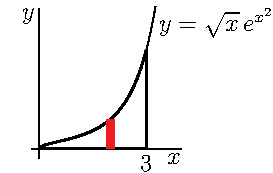
\includegraphics{OE00D_3b}
\end{center}

\noindent  is rotated about the $x$--axis, it
forms a thin disk of radius $\sqrt{x}e^{x^2}$  and thickness $\dee{x}$
and hence of cross sectional area $\pi xe^{2x^2}$ and volume $\pi xe^{2x^2}\,\dee{x}$
So the volume of the solid is
\begin{align*}
\pi\int_{0}^{3} xe^{2x^2}\ \dee{x}
\end{align*}


\noindent (b)
The curves intersect at $(-1,1)$ and $(2,4)$.

\begin{center}
       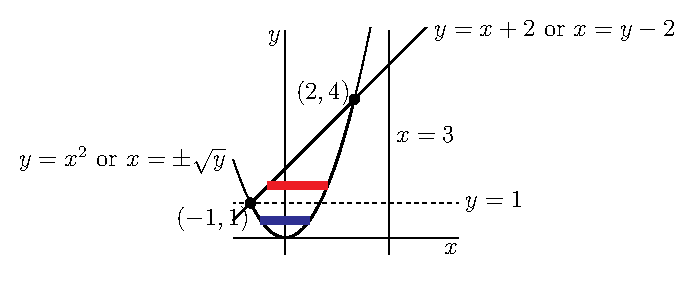
\includegraphics[scale=1.2]{OE00D_3e}
\end{center}

\noindent
We'll use horizontal washers as in Example  \eref{CLP101}{eg rot yaxis}
of the %\href{http://www.math.ubc.ca/%7Efeldman/m101/clp/clp_notes_101.pdf}{CLP 101 notes}.
CLP-2 text.
 \begin{itemize}
\item We use thin horizontal  strips of width $\dee{y}$ as in the figure  above.

\item When we rotate about the line $x=3$, each strip
sweeps out a thin washer
\begin{itemize}
\item
whose inner radius is $r_{in}=3-\sqrt{y}$, and
\item
whose outer radius is $r_{out}=3-(y-2)=5-y$ when $y\ge 1$
(see the red strip in the figure on the right above),  and
whose outer radius is $r_{out}= 3-(-\sqrt{y})=3+\sqrt{y}$ when $y\le 1$
(see the blue strip in the figure on the right above) and
\item
whose thickness is $\dee{y}$ and hence
\item
whose volume is
$\pi(r_{out}^2 - r_{in}^2)\dee{y}
       = \pi\big[\big(5-y\big)^2-\big(3-\sqrt{y}\big)^2\big]\dee{y}$
when $y\ge 1$ and  whose volume is
$\pi(r_{out}^2 - r_{in}^2)\dee{y}
    =\pi\big[\big(3+\sqrt{y}\big)^2-\big(3-\sqrt{y}\big)^2\big]\dee{y}$
when $y\le 1$ and

\end{itemize}
\item As our bottommost strip is at $y=0$ and our topmost
strip is at $y=4$, the total volume is
\begin{align*}
\int _0^1  \pi\big[\big(3+\sqrt{y}\big)^2-\big(3-\sqrt{y}\big)^2\big]\dee{y}
+\int _ 1^4  \pi\big[\big(5-y\big)^2-\big(3-\sqrt{y}\big)^2\big]\dee{y}
\end{align*}
\end{itemize}

\end{solution}
%%%%%%%%%%%%%%%%%%%%%%%%%%%%%%%%%%%%%%%%

\begin{Mquestion}[2001A,M121 2001A]  %% 2
Write down definite integrals that represent the following quantities.
\emph{Do not evaluate the integrals explicitly.}
\begin{enumerate}[(a)]
\item
The volume of the solid obtained by rotating the finite plane
region bounded by the curves $y=1-x^2$ and $y=4-4x^2$ about the line $y=-1$.
\item
The volume of the solid obtained by rotating the finite plane
region bounded by the curve $y=x^2-1$ and the line $y=0$ about the line $x=5$.
\end{enumerate}
\end{Mquestion}

\begin{hint}
Draw sketchs.
\end{hint}

\begin{answer} (a)
$\displaystyle\int_{-1}^{1}\pi\big[{(5-4x^2)}^2-{(2-x^2)}^2\big]\,\dee{x}$
\qquad (b)
$\displaystyle\int _{-1}^0   \pi\big[\big(5+\sqrt{y+1}\big)^2-\big(5-\sqrt{y+1}\big)^2\big]\,\dee{y}$

\end{answer}

\begin{solution} (a)
The curves intersect at $(1,0)$ and $(-1,0)$. When the strip shown in the
figure
\begin{center}
       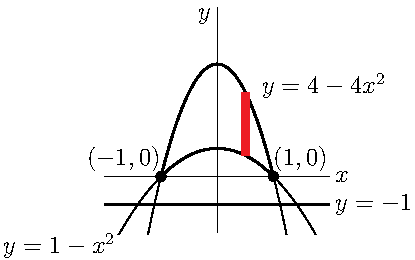
\includegraphics{OE01A_2b}
\end{center}

\noindent
is rotated about the line $y=-1$, it forms a thin washer with:
\begin{itemize}
\item
inner radius  $(1-x^2)-(-1)=2-x^2$,
\item
outer radius $(4-4x^2)-(-1)=5-4x^2$  and
\item thickness $\dee{x}$\ ; so, it has
\item
cross sectional area $\pi\big[{(5-4x^2)}^2-{(2-x^2)}^2\big]$ and
\item
volume $\pi\big[{(5-4x^2)}^2-({2-x^2)}^2\big]\,\dee{x}$.
\end{itemize}

\noindent So the volume of the solid is
\begin{align*}
\int_{-1}^{1}\pi\big[{(5-4x^2)}^2-{(2-x^2)}^2\big]\,\dee{x}
\end{align*}


\noindent (b)
The curve $y=x^2-1$ intersects $y=0$ at $(1,0)$ and $(-1,0)$.

\begin{center}
       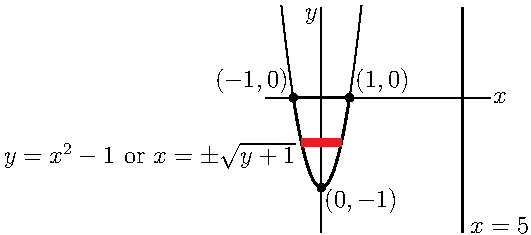
\includegraphics[scale=1.2]{OE01A_2c}
\end{center}

\noindent
We'll use horizontal washers.
 \begin{itemize}
\item We use thin horizontal  strips of height $\dee{y}$ as in the figure  above.

\item
When we rotate about the line $x=5$, each strip sweeps out a thin washer
\begin{itemize}
\item
whose inner radius is $r_{in}=5-\sqrt{y+1}$, and
\item
whose outer radius is $r_{out}= 5-(-\sqrt{y+1})=5+\sqrt{y+1}$ and
\item
whose thickness is $\dee{y}$ and hence
\item
whose volume is
$\pi(r_{out}^2 - r_{in}^2)\,\dee{y}
       = \pi\big[\big(5+\sqrt{y+1}\big)^2-\big(5-\sqrt{y+1}\big)^2\big]\,\dee{y}$

\end{itemize}
\item As our topmost strip is at $y=0$ and our bottommost
strip is at $y=-1$ (when $x=0$), the total volume is
\begin{align*}
\int _{-1}^0   \pi\left[\big(5+\sqrt{y+1}\big)^2-\big(5-\sqrt{y+1}\big)^2\right]\,\dee{y}
\end{align*}
\end{itemize}

\end{solution}
%%%%%%%%%%%%%%%%%%%%%%%%%%%%%%%%%%%%%%%%


\begin{question}[2001D] %% 3
Write down a definite integral that represents the volume of the solid
obtained by rotating  around the line $y=-1$ the region between the
curves $y=x^2$ and $y=8-x^2$.
\emph{Do not evaluate the integrals explicitly.}
\end{question}

\begin{hint}
Draw a sketch.
\end{hint}

\begin{answer}
$\pi\displaystyle\int_{-2}^{2}\big[{(9-x^2)}^2-{(x^2+1)}^2\big]\ \dee{x}$
\end{answer}

\begin{solution}
The curves intersect at $(-2,4)$ and $(2,4)$. When the strip
shown in the figure
\begin{center}
       
\includegraphics{OE01D_3b}
\end{center}

\noindent
is rotated about the line $y=-1$, it forms
a thin washer (punctured disc) of
\begin{itemize}
\item
inner radius $x^2+1$,
\item
outer radius $9-x^2$  and
\item thickness $\dee{x}$ and hence of
\item
cross sectional area $\pi\big[{(9-x^2)}^2-{(x^2+1)}^2\big]$ and
\item
volume $\pi\big[{(9-x^2)}^2-{(x^2+1)}^2\big]\,\dee{x}$.
\end{itemize}

\noindent So the volume of the solid is
\begin{align*}
\pi\int_{-2}^{2}\big[{(9-x^2)}^2-{(x^2+1)}^2\big]\ \dee{x}
\end{align*}
\end{solution}
%%%%%%%%%%%%%%%%%%%%%%%%%%%%%%%%%%%%%%%%

%%%-------all three parts were asked before
%\begin{question}[M121 2001A] %% 4
%Write definite integrals that represent the following quantities.
%\emph{Do not evaluate the integrals.}
%\begin{enumerate}[(a)]
%\item
%The area of the finite plane region bounded by $y^2=4ax$ and
%$x^2=4ay$, where $a>0$ is a constant.
%\item
%The volume of the solid obtained by rotating the finite plane
%region bounded by the curves $y=1-x^2$ and $y=4-4x^2$ about the line $y=-1$.
%\item
% The volume of the solid obtained by rotating the finite plane
%region bounded by the curve $y=x^2-1$ and the line $y=0$ about the line $x=5$.
%\end{enumerate}
%\end{question}

%\begin{hint}
%(a) Draw a sketch.
%\qquad
%(b) Draw a sketch.
%\qquad
%(c) Draw a sketch.
%\qquad
%See a pattern?
%\end{hint}

%\begin{answer}
%(a) $\displaystyle\int_0^{4a}\left[\sqrt{4ax}-\frac{x^2}{4a}\right]\ \dee{x}$
%\qquad
%(b) $\displaystyle\int_{-1}^{1}\pi\big[{(5-4x^2)}^2-{(2-x^2)}^2\big]\ \dee{x}$

%\noindent
%(c) $\displaystyle\int_{-1}^0\pi\big[{(5+\sqrt{y+1})}^2-{(5-\sqrt{y+1})}^2\big]\ \dee{y}
%=\displaystyle\int_{-1}^020\pi\sqrt{y+1}\,\dee{y}$
%\end{answer}

%\begin{solution} (a) (This was also calculated in Section 1.5, Question~\ref{1.5_4ax4ay}.)
%The curves intersect at points $(x,y)$ which satisfy both
%$y^2=4ax$ and $x^2=4ay$. Substituting $y=\frac{x^2}{4a}$ (from
%the second equation) into the first equation gives
%\begin{equation*}
%\frac{x^4}{4^2a^2}=4ax
%\iff x^4=4^3a^3x
%\iff x(x^3-4^3a^3)=0
%\end{equation*}
%This has two solutions: $x=0$ and $x=4a$. The corresponding values
%of $y$ are $y=0$ and $y=4a$. So the curves intesect at $(0,0)$ and $(4a,4a)$.
%The strip shown in the figure

%\begin{center}
%       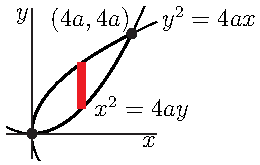
\includegraphics{E121_01A_1a}
%\end{center}

%\noindent runs from $y=B(x) = \frac{x^2}{4a}$ (gotten by solving
%$x^2=4ay$ for $y$) to $y=T(x)= \sqrt{4ax}$
%(gotten by solving $y^2=4ax$ for $y$) and hence has height
%$T(x)-B(x) = \sqrt{4ax}-\frac{x^2}{4a}$ and width $\dee{x}$.
%So the desired
%\begin{equation*}
%{\rm Area} = \int_0^{4a}\Big[\sqrt{4ax}-\frac{x^2}{4a}\Big]\ \dee{x}
%\end{equation*}

%\noindent (b)
%The curves intersect at points $(x,y)$ which satisfy both
%$y=1-x^2$ and $y=4(1-x^2)$. That is, where
%\begin{equation*}
%1-x^2=4(1-x^2)
%\iff 3(1-x^2)=0\iff x=\pm 1
%\end{equation*}
%Thus the curves intersect at $(1,0)$ and $(-1,0)$. When the strip
%shown in the figure

%\begin{center}
%       \includegraphics{E121_01A_1b}
%\end{center}

%\noindent
%is rotated about the line $y=-1$, it forms
%a thin washer (punctured disc) of
%\begin{itemize}
%\item
%inner radius $(1-x^2)-(-1)=2-x^2$,
%\item
%outer radius $(4-4x^2)-(-1)=5-4x^2$  and
%\item thickness $\dee{x}$ and hence of
%\item
%cross sectional area $\pi\big[{(5-4x^2)}^2-{(2-x^2)}^2\big]$ and
%\item
%volume $\pi\big[{5-4x^2)}^2-{(2-x^2)}^2\big]\,\dee{x}$.
%\end{itemize}

%\noindent So the volume of the solid is
%\begin{align*}
%\int_{-1}^{1}\pi\big[{(5-4x^2)}^2-{(2-x^2)}^2\big]\ \dee{x}
%\end{align*}


%\noindent (c)
%Note that solving $y=x^2-1$ for $x$ gives $x=\pm\sqrt{y+1}$.
%When the strip shown in the figure

%\begin{center}
%       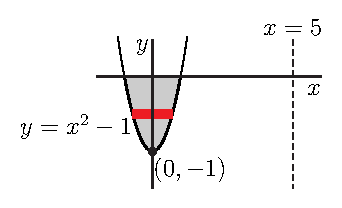
\includegraphics{E121_01A_1c}
%\end{center}

%\noindent
%is rotated about the line $x=5$, it forms
%a thin washer (punctured disc) of
%\begin{itemize}
%\item
%inner radius $5-\sqrt{y+1}$,
%\item
%outer radius $5+\sqrt{y+1}$  and
%\item thickness $\dee{y}$ and hence of
%\item
%cross sectional area $\pi\big[{(5+\sqrt{y+1})}^2-{(5-\sqrt{y+1})}^2\big]
%=20\pi\sqrt{y+1}$ and
%\item
%volume $\pi\big[{(5+\sqrt{y+1})}^2-{(5-\sqrt{y+1})}^2\big]\,\dee{y}
%=20\pi\sqrt{y+1}\,\dee{y}$.
%\end{itemize}

%\noindent So the volume of the solid is
%\begin{align*}
%\int_{-1}^0\pi\big[{(5+\sqrt{y+1})}^2-{(5-\sqrt{y+1})}^2\big]\ \dee{y}
%=\int_{-1}^020\pi\sqrt{y+1}\,\dee{y}
%\end{align*}


%\end{solution}
%%%%%%%%%%%%%%%%%%%%%%%%%%%%%%%%%%%%%%%%





%%%%%%%%%%%%%%%%%%%%%%%%%%%%%%%%%%%%%
\begin{question}
A tetrahedron is a three-dimensional shape with four faces, each of which is an equilateral triangle. (You might have seen this shape as a 4-sided die; think of a pyramid with a triangular base.) Using the methods from this section, calculate the volume of a tetrahedron with side-length $\ell$. You may assume without proof that the height of a tetrahedron with side-length $\ell$ is $\sqrt{\frac{2}{3}}\ell$.

\begin{center}
\begin{tikzpicture}
\draw (0,0) coordinate(a0);
\draw (3,0) coordinate(a1);
\draw (2,-.75) coordinate(a2);
\draw (1.8,2.) coordinate(a3);
\draw[dashed, gray] (a0)--(a1);
\draw[fill, fill opacity=0.3] (a2)--(a3)--(a1)--cycle;
\draw[fill, fill opacity=0.1] (a0)--(a3)--(a2)--cycle;
\draw[decorate, decoration={brace, amplitude=10pt}] (-.2,0.2)--(1.6,2.2) node[midway, above left, xshift=-7pt]{$\ell$};
\draw[decorate, decoration={brace, amplitude=10pt, mirror}] (3.5,0)--(3.5,2) node[midway,  right, xshift=7pt]{$\sqrt{\frac{2}{3}}\ell$};

\end{tikzpicture}
\end{center}
\end{question}
\begin{hint}
If you take horizontal slices (parallel to one face), they will all be equilateral triangles.

Be careful not to confuse the height of a \emph{triangle} with the height of the tetrahedron.
\end{hint}
\begin{answer}
$\dfrac{\sqrt{2}}{12}\ell^3$
\end{answer}
\begin{solution}
We'll make horizontal slices, parallel to one of the faces of the tetrahedron. Then our slices will be equilateral triangles, of varying sizes.

\begin{center}
\begin{tikzpicture}
\draw (0,0) coordinate(a0);
\draw (3,0) coordinate(a1);
\draw (2,-.75) coordinate(a2);
\draw (1.8,2.) coordinate(a3);
\filldraw[fill opacity=0.5] (0.9,1)--(2.4,1)--(1.9,0.625)--cycle;
\filldraw[fill opacity=0.2] (0.9,1)--(0.9,0.8)--(1.9,0.425)--(2.4,.8)--(2.4,1)--cycle;
\draw[dashed, gray] (a0)--(a1);
\draw[fill, fill opacity=0.3] (a2)--(a3)--(a1)--cycle;
\draw[fill, fill opacity=0.1] (a0)--(a3)--(a2)--cycle;
\draw[decorate, decoration={brace, amplitude=10pt}] (-.2,0.2)--(1.6,2.2) node[midway, above left, xshift=-7pt]{$\ell$};
\end{tikzpicture}
\end{center}



 For the sake of ease, as in Example \eref{CLP101}{eg:VOLa} of the CLP-2 text,
we picture the tetrahedron perched on a tip, one base horizontal on top.

%Note that the height of an equilateral triangle with side-length $\ell$ is $\sqrt{\frac{2}{3}}\ell$ (which we find using the Pythagorean Theorem). Then at height $y$, the length of the side of an equilateral triangular cross-section is $\frac{2}{\sqrt{3}}y$, and its area is $\frac{1}{2}y\left(\frac{2}{\sqrt{3}}y\right)=\frac{y^2}{\sqrt{3}}$.
\begin{center}
\begin{tikzpicture}
\YEaaxis{3}{3}{1}{5}
\fill[fill opacity=0.1] (-1.84,2.8)--(0,3.3)--(1.84,2.8)--cycle;

\draw[thick](-1.2,3.8)-- (-2.5,3.8)--(0,0)--(2.5,3.8)--(-.2,3.8);
\YEycoord{3}{y}
\YEycoord{4.08}{\sqrt{\frac{2}{3}}\ell}
\YExcoord{2.5}{\frac{\ell}{2}}
\YExcoord{-2.5}{-\frac{\ell}{2}}
%\draw (-1.84,3)--(-.75,3) (.3,3)--(1.84,3);
%\draw (0,0)--(2.5,3.9)--(2.5,4.08);
\draw (-2.5,3.8)-- (0,4.5)--(2.5,3.8);
\end{tikzpicture}
\end{center}

Notice our slice forms the horizontal top of a smaller tetrahedron. The horizontal top of the full tetrahedron has side length $\ell$, which is
             $\sqrt{\frac{3}{2}}$ times the height of the full tetrahedron. Our slice
             is the horizontal top of a tetrahedron of height $y$ and so has side length  $\sqrt{\frac{3}{2}}y$. An equilateral triangle with side length $L$ has base $L$ and height
              $\frac{\sqrt{3}}{2}L$, and hence area $\frac{\sqrt{3}}{4}L^2$.
             So, the area of our slice with side length $\sqrt{\frac{3}{2}}y$ is
\[A = \frac{\sqrt{3}}{4}\left(\sqrt{\frac{3}{2}}y\right)^2 = \frac{3\sqrt{3}}{8}y^2\]

So, the volume of a tetrahedron with side length $\ell$ is:
\begin{align*}
\mbox{Volume}&=\int_0^{\sqrt{\frac{2}{3}}\ell}\frac{3\sqrt{3}}{8}y^2\ \dee{y}\\
&=\frac{\sqrt{3}}{8}\cdot \left(\sqrt{\frac{2}{3}}\ell\right)^3=\frac{\sqrt{2}}{12}\ell^3
\end{align*}



\emph{You were given the height of a tetrahedron, but for completeness we calculate it here.}


Draw a line starting at one tip, and dropping straight down to the middle of the opposite face. It forms a right triangle with one edge of the tetrahedron, and a line from the middle of the face to the corner.


\begin{center}
\begin{tikzpicture}[scale=1.5]
\draw (0,0) coordinate(a0);
\draw (3,0) coordinate(a1);
\draw (2,-.75) coordinate(a2);
\draw (1.8,2.) coordinate(a3);
\draw[dashed, gray] (a0)--(a1);
\draw[fill, fill opacity=0.3] (a2)--(a3)--(a1)--cycle;
\draw[fill, fill opacity=0.1] (a0)--(a3)--(a2)--cycle;
\draw[decorate, decoration={brace, amplitude=10pt}] (-.2,0.2)--(1.6,2.2) node[midway, above left, xshift=-7pt]{$\ell$};
\draw[thick, densely dotted] (1.8,2)--(1.7,-.3)--(a0);
\draw(1.7,-.3) node[vertex, label=below:$c$]{};
\draw (a0) node[left]{$A$};
\draw (a1) node[right]{$C$};
\end{tikzpicture}
\end{center}

We know the length of the hypotenuse of this right triangle (it's $\ell$), so if we know the length of its base (labeled $Ac$ in the diagram), we can figure out its third side, the height of our tetrahedron. Note by using the Pythagorean theorem, we see that the height of an equilateral triangle with edge length $\ell$ is $\sqrt{\frac{3}{2}}\ell$.

Here is a sketch of the base of the pyramid:

\begin{center}
\begin{tikzpicture}
\draw node[vertex]{};
\foreach \x in {0,1,2}{
	\draw (0,0) + (30+120*\x:3cm) node[vertex](v\x){};}
\draw (v1) node[left]{$A$};
\draw (v0) node[right]{$C$};
\draw (v0)--(v1)--(v2)--(v0);
\draw (v0)--(v2) coordinate[midway, label=right:{$B$}](m0){};
\draw (v1)--(v0) coordinate[midway, label=above:{$b$}](m2){};
\draw (v1)--(m0);
\draw (0,0)--(m2);
\draw  node[below]{$c$};
\draw  (-1,-1.5) node[below]{$\ell$};
\end{tikzpicture}
\end{center}

The triangles $ABC$ and $Abc$ are similar (since $b$ and $B$ are right angles, and also $A$ has the same angle in both). Therefore,
\begin{align*}
\frac{{Ac}}{{Ab}}&=\frac{{AC}}{{AB}}\\
\frac{Ac}{\ell/2}&=\frac{\ell}{\sqrt{3}\ell/2}\\
Ac&=\frac{1}{\sqrt{3}}\ell
\end{align*}

With this in our pocket, we can find the height of the tetrahedron: $\sqrt{\ell^2 - \left(\frac{1}{\sqrt{3}}\ell\right)^2} =\sqrt{\frac{2}{3}}\ell$.


\end{solution}


%%%%%%%%%%%%%%%%%%
\subsection*{\Procedural}
%%%%%%%%%%%%%%%%%%

\begin{Mquestion}[2016Q3] %% 5
Let $a>0$ be a constant. Let $R$ be the finite region bounded by the
graph of $y=1+\sqrt{x}e^{x^2}$, the line $y=1$, and the line $x=a$. Using
vertical slices, find the volume generated when $R$ is rotated about the line $y=1$.
\end{Mquestion}

\begin{hint}
Sketch the region.
\end{hint}

\begin{answer}
$\displaystyle\frac{\pi}{4}\Big(e^{2a^2}-1\Big)$
\end{answer}

\begin{solution}
Let $f(x)=1+\sqrt{x}e^{x^2}$.
On the vertical slice a distance $x$ from the $y$-axis,
sketched in the figure below, $y$ runs from $1$ to $f(x)$. Upon rotation
about the line $y=1$, this thin slice sweeps out a thin disk of thickness
$\dee{x}$ and radius $f(x)-1$ and hence of volume $\pi[f(x)-1]^2\,\dee{x}$.
The full volume generated (for any fixed $a>0$) is
\begin{align*}
\int_0^a\pi[f(x)-1]^2\,\dee{x}
=\pi\int_0^axe^{2x^2}\,\dee{x}.
\end{align*}
Using the substitution $u=2x^2$, so that $\dee{u}=4x\,\dee{x}$:
\begin{align*}
\text{Volume} = \pi\int_0^{2a^2}e^u\,\frac{\dee{u}}{4}
=\frac{\pi}{4}e^u\Big|_0^{2a^2}
=\frac{\pi}{4}\Big(e^{2a^2}-1\Big)
\qquad\qquad\smash{\raisebox{-0.4\height}{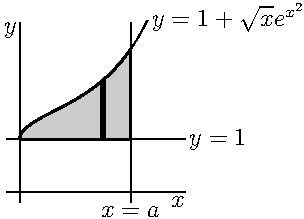
\includegraphics{OQ16_3_4b}}}
\end{align*}

\vspace{1cm}
Remark: we spent a good deal of time last semester developing highly accurate but time-consuming methods for sketching common functions. For the purposes of questions like this, we don't need a detailed picture of a function--broad outlines suffice. Notice that $\sqrt{x} > 0$ whenever $x>0$, and $e^{x^2}>0$ for all $x$. Therefore, $\sqrt{x}e^{x^2}$ is nonnegative over its entire domain, and so the graph $y=1+\sqrt{x}e^{x^2}$ is always the top function, above the bottom function $y=1$. That is the only information we needed to perform our calculation.
\end{solution}
%%%%%%%%%%%%%%%%%%%





\begin{question}[2014A] %% 7
Find the volume of the solid generated by rotating the finite
region bounded by $y = 1/x$ and $3x + 3y = 10$ about the $x$--axis.
\end{question}

\begin{hint}
Sketch the region first.
\end{hint}

\begin{answer}
$\pi\left[\dfrac{38}{3}-\dfrac{514}{3^4}\right] = \pi\dfrac{512}{81}$
\end{answer}

\begin{solution}

The curves $y=1/x$ and $3x+3y=10$, i.e. $y =\frac{10}{3}-x$ intersect
when
\begin{align*}
\frac{1}{x} = \frac{10}{3}-x
&\iff 3 = 10x-3x^2
\iff 3x^2-10x+3=0 \\
&\iff(3x-1)(x-3)=0 \\
&\iff x=3\,,\,\frac{1}{3}
\end{align*}

\smallskip
\centerline{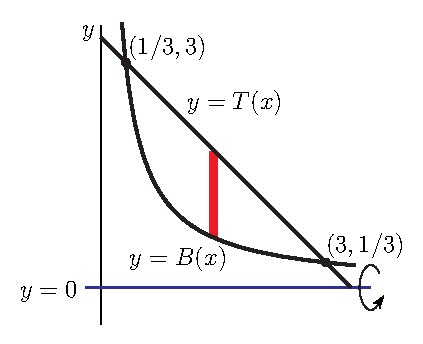
\includegraphics[scale=1.0]{OE14A_3}}
\smallskip

\noindent
When the region is rotated about the $x$--axis, the vertical strip
in the figure above sweeps out a washer with thickness $\dee{x}$,
outer radius $T(x)=\frac{10}{3}-x$ and inner radius $B(x)=\frac{1}{x}$.
This washer has volume
\begin{equation*}
\pi\big(T(x)^2- B(x)^2\big)\,\dee{x}
= \pi\Big(\frac{100}{9}-\frac{20}{3}x+x^2-\frac{1}{x^2}\Big)\,\dee{x}
\end{equation*}
Hence the volume of the solid is
\begin{align*}
\pi\int_{1/3}^3\Big(\frac{100}{9}-\frac{20}{3}x+x^2-\frac{1}{x^2}\Big)\,\dee{x}
&=\pi\Big[\frac{100x}{9}-\frac{10}{3}x^2+\frac{1}{3}x^3
              +\frac{1}{x}\Big]_{1/3}^3 \\
&=\pi\Big[\frac{38}{3}-\frac{514}{3^4}\Big] = \pi\frac{512}{81}
\end{align*}
\end{solution}
%%%%%%%%%%%%%%%%%%%


\begin{question}[2015A] %% 8
 Let $R$ be the region inside the circle $x^2 + (y-2)^2=1$. Let $S$ be the solid obtained by rotating $R$ about the $x$-axis.
\begin{enumerate}[(a)]
\item
 Write down an integral representing the volume of $S$.
\item
Evaluate the integral you wrote down in part (a).
\end{enumerate}
\end{question}

\begin{hint}
You can save yourself quite a bit of work by interpreting the integral
as the  area of a known geometric figure.
\end{hint}

\begin{answer} (a)
$8\pi\int_{-1}^1\sqrt{1-x^2}\,\dee{x}$
\qquad (b)
$ 4\pi^2$
\end{answer}

\begin{solution} (a)
The top and the bottom of the circle have equations
$y=T(x)=2+\sqrt{1-x^2}$ and $y=B(x) = 2-\sqrt{1-x^2}$, respectively.

\smallskip
\centerline{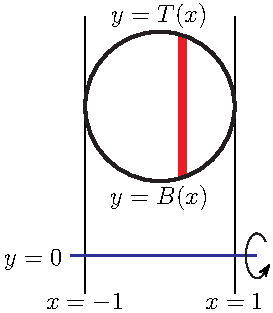
\includegraphics{OE15A_10}}
\smallskip

\noindent
When $R$ is rotated about the $x$--axis, the vertical strip of
$R$ in the figure above sweeps out a washer with thickness $\dee{x}$,
outer radius $T(x)$ and inner radius $B(x)$. This washer has
volume
\begin{equation*}
\null\hskip0.5in\pi\big(T(x)^2- B(x)^2\big)\,\dee{x}
= \pi\big(T(x)+ B(x)\big)\big(T(x)- B(x)\big)\,\dee{x}
= \pi\times 4\times 2\sqrt{1-x^2}\,\dee{x}
\end{equation*}
Hence the volume of the solid is
\begin{equation*}
8\pi\int_{-1}^1\sqrt{1-x^2}\,\dee{x}
\end{equation*}

\noindent (b)
Since $y=\sqrt{1-x^2}$ is equivalent to $x^2+y^2=1$, $y\ge 0$,
the integral is $8\pi$ times the area of the upper half
of the circle $x^2+y^2=1$ and hence is
$8\pi\times \frac{1}{2}\pi 1^2 = 4\pi^2$.


\end{solution}
%%%%%%%%%%%%%%%%%%%

\begin{question}[1996D] %% 9
 The region $R$ is the portion of the first quadrant which
is below the parabola $y^2=8x$ and above the hyperbola $y^2-x^2=15$.
\begin{enumerate}[(a)]
\item
Sketch the region $R$.
\item
Find the volume of the solid obtained by revolving $R$ about the $x$ axis.
\end{enumerate}
\end{question}

\begin{hint}
See Example \eref{CLP101}{eg:VOLe} in the
%\href{http://www.math.ubc.ca/%7Efeldman/m101/clp/clp_notes_101.pdf}{CLP 101 notes}.
CLP-2 text.
\end{hint}

\begin{answer} (a)
The region $R$ is the region
between the blue and red curves, with $3\le x\le 5$,  in the figures below.

\begin{center}
       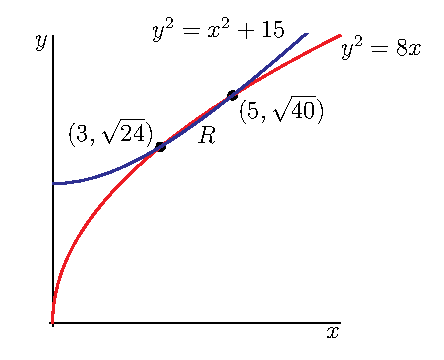
\includegraphics{graphE1}\qquad
       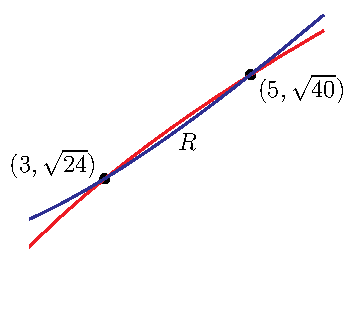
\includegraphics{graphE1b}
\end{center}

\noindent (b) $\frac{4}{3}\pi\approx 4.19$
\end{answer}

\begin{solution} (a)
The two curves intersect when $x$ obeys $8x=x^2+15$
or $x^2-8x+15=(x-5)(x-3)=0$. The points of intersection, in the first quadrant,
are $(3,\sqrt{24})$ and $(5, \sqrt{40})$. The region $R$ is the region
between the blue and red curves, with $3\le x\le 5$,  in the figures below.

\begin{center}
       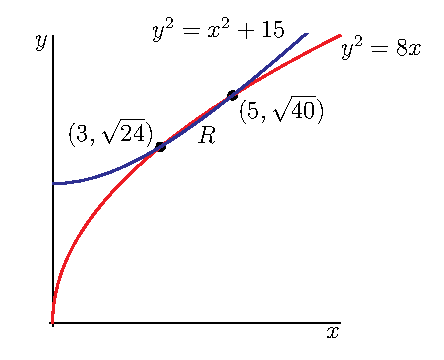
\includegraphics{graphE1}\qquad
       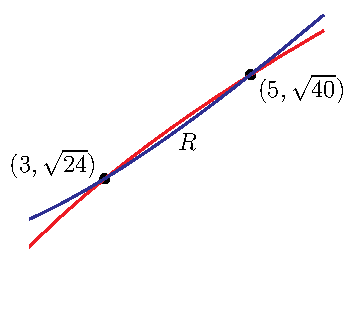
\includegraphics{graphE1b}
\end{center}

\item{}(b) The part of the solid with $x$ coordinate between $x$ and $x+\dee{x}$
is a ``washer'' shaped region with inner radius $\sqrt{x^2+15}$, outer
radius $\sqrt{8x}$ and thickness $\dee{x}$. The surface area of the washer is
$\pi(\sqrt{8x})^2 -\pi(\sqrt{x^2+15})^2=\pi(8x-x^2-15)$ and its volume is
$\pi(8x-x^2-15)\,\dee{x}$. The total volume is
\begin{align*}
\int_3^5 \pi(8x-x^2-15)\,\dee{x}
&=\pi\Big[4x^2-\frac{1}{3}x^3-15 x\Big]_3^5
=\pi\Big[100-\frac{125}{3}-75-36+9+45\Big] \\
&=\frac{4}{3}\pi\approx 4.19
\end{align*}

\end{solution}
%%%%%%%%%%%%%%%%%%%


\begin{Mquestion}[1996D] %% 10
 The region $R$ is bounded by $y=\log x$, $y=0$, $x=1$ and $x=2$.
(Recall that we are using $\log x$ to denote the logarithm of $x$ with
base $e$. In other courses it is often denoted $\log x$.)
\begin{enumerate}[(a)]
\item
Sketch the region $R$.
\item
Find the volume of the solid obtained by revolving this region  about the $y$ axis.
\end{enumerate}
\end{Mquestion}

\begin{hint}
See Example \eref{CLP101}{eg rot yaxis} in the
%\href{http://www.math.ubc.ca/%7Efeldman/m101/clp/clp_notes_101.pdf}{CLP 101 notes}.
CLP-2 text.
\end{hint}

\begin{answer} (a)
The region $R$ is sketched below.

\begin{center}
       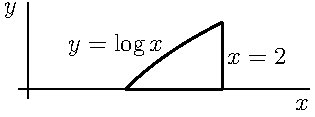
\includegraphics{graphE2l}
\end{center}

\noindent (b) $\pi\Big[4\log 2 - \frac{3}{2}\Big] \approx 3.998$
\end{answer}

\begin{solution} (a)
The region $R$ is sketched in the figure on the left below. (The bound $y=0$ renders the bound $x=1$ unnecessary, since the graph $y=\log x$ hits the $x$-axis when $x=1$.)

\begin{center}
       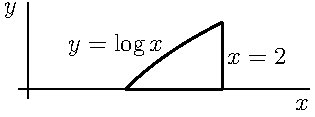
\includegraphics{graphE2l}\qquad
       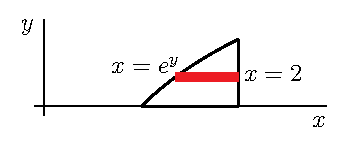
\includegraphics{graphE2r}
\end{center}

\noindent (b)
We'll use horizontal washers as in Example  \eref{CLP101}{eg rot yaxis}
of the %\href{http://www.math.ubc.ca/%7Efeldman/m101/clp/clp_notes_101.pdf}{CLP 101 notes}.
CLP-2 text.
 \begin{itemize}
\item We cut $R$ into thin horizontal  strips of height $\dee{y}$ as in
the figure on the right above.

\item When we rotate $R$ about the $y$--axis, i.e. about the line $x=0$,
each strip sweeps out a thin washer
\begin{itemize}
\item whose inner radius is $r_{in}= e^y$ and outer radius is $r_{out}=2$, and
\item whose thickness is $\dee{y}$ and hence
\item whose volume $\pi(r_{out}^2 - r_{in}^2)\dee{y} = \pi\big(4-e^{2y}\big)\dee{y}$.
\end{itemize}
\item As our bottommost strip is at $y=0$ and our topmost
strip is at $y=\log 2$ (since at the top $x=2$ and $x=e^y$), the total
\begin{align*}
\text{Volume}
&= \int _0^{\log 2} \pi\big(4-e^{2y}\big)\ \dee{y}
=\pi\big[4y -e^{2y}/2\big]_0^{\log 2}
=\pi\Big[4\log 2 - 2 +\frac{1}{2}\Big] \\
&=\pi\Big[4\log 2 - \frac{3}{2}\Big]
\end{align*}
Using a calculator, we see this is approximately $3.998$.
\end{itemize}
\end{solution}
%%%%%%%%%%%%%%%%%%%

\begin{question}[2016Q3] %% 11
The finite region between the curves $y = \cos(\frac x2)$
and $y = x^2 - \pi^2$ is rotated about the line $y=-{\pi^2}$.
Using vertical slices (disks and/or washers), find the volume of
the resulting solid.
\end{question}

\begin{hint}
Sketch the region. To find where the curves intersect, look at where
$\cos(\frac x2)$ and $x^2 - \pi^2$  both have roots.
\end{hint}

\begin{answer}
 $\pi^2 + 8\pi^3 + \frac{8\pi^6}{5}$
\end{answer}

\begin{solution}
Here is a sketch of the curves $y = \cos(\frac x2)$ and $y = x^2 - \pi^2$.

\begin{center}
       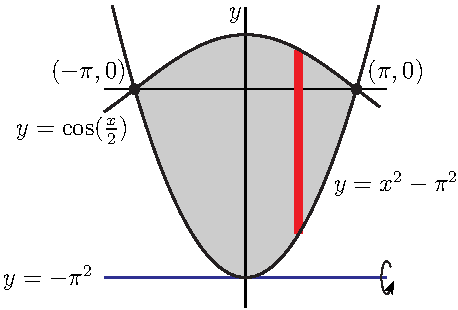
\includegraphics{OQ16_3_4}
\end{center}

By inspection, the curves meet at $x = \pm {\pi}$ where both $\cos(\frac x2)$  and
$x^2 - \pi^2$ take the value zero.
We'll use vertical washers as specified in the question.
 \begin{itemize}
\item We cut the specified region into thin vertical strips of
width $\dee{x}$ as in the figure above.

\item When we rotate about the line $y=-\pi^2$,
each strip sweeps out a thin washer
\begin{itemize}
\item whose inner radius is $r_{in}= (x^2 - {\pi^2} ) - ( {-} {\pi^2} )=x^2$
and outer radius is $r_{out}=\cos(\frac x2) - ( {-} {\pi^2})
=\cos(\frac x2) +\pi^2 $, and
\item whose thickness is $\dee{x}$ and hence
\item whose volume
    $\pi(r_{out}^2 - r_{in}^2)\dee{x}
        =  \pi\big( {(\cos(\frac x2) +\pi^2)}^2 - {(x^2)}^2\big)\dee{x}$.
\end{itemize}
\item As our leftmost strip is at $x=-\pi$ and our rightmost
strip is at $x=\pi$,
\end{itemize}
the total volume is
\begin{align*}
  &\pi \int_{-\pi}^{\pi}
         \left(  \cos^2 (\tfrac x2) +2{\pi^2}\cos (\tfrac x2) +{\pi^4} -x^4\right)\,\dee{x} \\
 &\hskip0.5in = \pi \int_{-\pi}^{\pi}
         \left(\frac{1+\cos(x)}{2} +2{\pi^2}\cos (\tfrac x2) +{\pi^4} -x^4\right)\,\dee{x}
         \intertext{Because the integrand is even,}
 &\hskip0.5in = 2\pi \int_0^{\pi}
         \left(\frac{1+\cos(x)}{2} +2{\pi^2}\cos (\tfrac x2) +{\pi^4} -x^4\right)\,\dee{x} \\
 &\hskip0.5in = {2\pi \left[ \frac{1}{2}x + \frac{1}{2}\sin(x)
          + 4{\pi^2}\sin (\tfrac x2)  +{\pi^4} x -\frac{1}{5}x^5   \right]} _0^\pi\\
 &\hskip0.5in = 2\pi \left[\frac{\pi}{2} + 0 + 4{\pi^2} +{\pi^5} - \frac{\pi^5}{5} \right] \\
 &\hskip0.5in = {\pi^2} + 8\pi^3 + \frac{8\pi^6}{5}
\end{align*}
We used the fact that the integrand is an even function and the interval of integration $[-\pi, \pi]$ is symmetric, but one can also compute directly.

%\centerline{
%\begin{tikzpicture}
%\draw[domain=-2.00:2.00,dashed] plot (\x,{cos(\x r)});
%\draw[domain=-2.00:2.00,dashed] plot (\x,{\x*\x-2.47});
%\draw[domain=-1.57:1.57] plot (\x,{cos(\x r)});
%\draw[domain=-1.57:1.57] plot (\x,{\x*\x-2.47});
%\draw[dashed] (-2.5,-2.47) -- (2.5,-2.47);
%\node at (-1.5,-2.8) {$y = -\pi^2$};
%\draw (+1.57,0) -- (+1.57,-0.2) node[below] {${\pi}$};
%\draw (-1.57,0) -- (-1.57,-0.2) node[below] {$-{\pi}$};
%\draw[ultra thick,->] (-2.5,0) -- (2.5,0);
%\draw[ultra thick,->] (0,-3.5) -- (0,3);
%\end{tikzpicture}
%}
\end{solution}
%%%%%%%%%%%%%%%%%%%


\begin{Mquestion}[1997D] %% 12
The solid $V$ is 2 meters high and has square horizontal
cross sections. The length of the side of the square cross section at height
$x$ meters above the base is $\frac{2}{1+x}$ m. Find the volume
of this solid.
\end{Mquestion}

\begin{hint}
See Example \eref{CLP101}{eg:VOLb} in the
%\href{http://www.math.ubc.ca/%7Efeldman/m101/clp/clp_notes_101.pdf}{CLP 101 notes}.
CLP-2 text.
\end{hint}

\begin{answer}
$\dfrac{8}{3}$
\end{answer}

\begin{solution}
As in Example \eref{CLP101}{eg:VOLb} of the
%\href{http://www.math.ubc.ca/%7Efeldman/m101/clp/clp_notes_101.pdf}{CLP 101 notes}.
CLP-2 text notes, we slice $V$  into thin horizontal ``square pancakes''.

\begin{itemize}
\item We are told that the pancake at height $x$ is a square
of side $\frac{2}{1+x}$ and so
\item has cross-sectional area $\big(\frac{2}{1+x}\big)^2$ and
thickness $\dee{x}$ and hence
\item has volume $\big(\frac{2}{1+x}\big)^2\dee{x}$.
\end{itemize}
\noindent Hence the volume of $V$ is
$$
\int_0^2{\Big[\frac{2}{1+x}\Big]}^2\,\dee{x}
=\int_1^3\frac{4}{u^2}\,\dee{u}
=4\frac{u^{-1}}{-1}\bigg|_1^3
=-4\Big[\frac{1}{3}-1\Big]
=\frac{8}{3}
$$
We made the change of variables $u=1+x$, $\dee{u}=\dee{x}$.
\end{solution}
%%%%%%%%%%%%%%%%%%%

\begin{question}[1998A] %% 13
Consider a solid whose base is the finite portion of the
$xy$--plane bounded by the curves $y=x^2$ and $y=8-x^2$. The cross--sections
perpendicular to the $x$--axis are squares with one side in the $xy$--plane.
Compute the volume of this solid.
\end{question}

\begin{hint}
See Example \eref{CLP101}{eg:VOLb} in the
%\href{http://www.math.ubc.ca/%7Efeldman/m101/clp/clp_notes_101.pdf}{CLP 101 notes}.
CLP-2 text. Imagine cross-sections with shadow parallel to the $y$-axis, sticking straight out of the $xy$-plane.
\end{hint}

\begin{answer}
 $\dfrac{256\times 8}{15}=136.5\dot3$
\end{answer}

\begin{solution}
Here is a sketch of the base region.

\begin{center}
       
\includegraphics{graphE98A_7}
\end{center}

\noindent
Consider the thin vertical cross--section resting on the heavy red
line in the figure above. It has thickness $\dee{x}$. Its face is a square
whose side runs from $y=x^2$ to $y=8-x^2$, a distance of $8-2x^2$. So the
face has area ${(8-2x^2)}^2$ and the slice has volume ${(8-2x^2)}^2\,\dee{x}$. The two
curves cross when $x^2=8-x^2$, i.e. when $x^2=4$ or $x=\pm 2$. So $x$ runs
from $-2$ to $2$ and the total volume is
\begin{align*}
\int_{-2}^{2}{(8-2x^2)}^2\,\dee{x}&=2\int_0^2 4{(4-x^2)}^2\,\dee{x}
=8\int_0^2\big[16-8x^2+x^4\big]\,\dee{x}\cr
&=8\Big[16\times 2-\frac{8}{3}2^3+\frac{1}{5}2^5\Big]
=\frac{256\times 8}{15}=136.5\dot3
\end{align*}
In the first simplification step, we used the fact that our integrand was even, but we also could have finished our computation without this step.
\end{solution}
%%%%%%%%%%%%%%%%%%%

\begin{Mquestion}[2001D] %% 14
A frustrum of a right circular cone (as shown below) has
height $h$. Its base is a circular disc with radius $4$ and its top is
a circular disc with radius $2$. Calculate the volume of the frustrum.
\begin{center}
       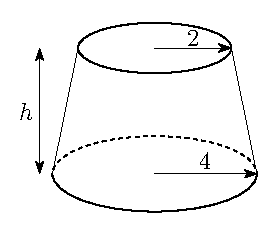
\includegraphics{OE01D_4b}
\end{center}
\end{Mquestion}

\begin{hint}
See Example \eref{CLP101}{eg:VOLa} in the
%\href{http://www.math.ubc.ca/%7Efeldman/m101/clp/clp_notes_101.pdf}{CLP 101 notes}.
CLP-2 text.
\end{hint}

\begin{answer}
$\dfrac{28}{3}\pi h$
\end{answer}

\begin{solution}
Slice the frustrum into horizontal discs. When the disc is a distance
$t$ from the top of the frustrum it has radius $2+2t/h$. Note that as $t$
runs from $0$ (the top of the frustrum) to $t=h$ (the bottom of the frustrum)
the radius $2+2t/h$ increases linearly from $2$ to $4$.
\begin{center}
       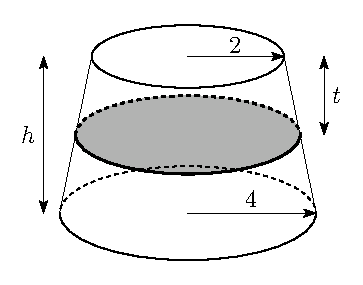
\includegraphics{OE01D_4}
\end{center}
 Thus the disk has volume $\pi \big(2+2t/h\big)^2 \dee{t}$. The total volume of the
frustrum is
\begin{align*}
\pi\int_0^h \big(2+2t/h\big)^2 \dee{t}
=4\pi\int_0^h \big(1+t/h\big)^2 \dee{t}
=4\pi\left[\frac{(1+t/h)^3}{3/h}\right]_0^h
=\frac{4}{3}\pi h\times 7
=\frac{28}{3}\pi h
\end{align*}

Remark: we could also solve this problem using the formula for the volume of a cone. Using similar triangles, the frustrum in question is shaped like a right circular cone of height $2h$ and base radius 4 (and hence of volume $\dfrac{1}{3}\pi(4^2)(2h)$), but missing its top, which is a right circular cone of height $h$ and base radius $2$ (and hence volume $\dfrac{1}{3}\pi(2^2)h$). So, the volume of the frustrum is $\dfrac{1}{3}\pi(4^2)(2h) - \dfrac{1}{3}\pi(2^2)h = \dfrac{28}{3}\pi h$.
\end{solution}
%%%%%%%%%%%%%%%%%%%







%%%%%%%%%%%%%%%%%%
\subsection*{\Application}
%%%%%%%%%%%%%%%%%%

\begin{question}
The shape of the earth is often approximated by an oblate spheroid, rather than a sphere. An \emph{oblate spheroid} is formed by rotating an ellipse about its \emph{minor axis} (its shortest diameter).
\begin{enumerate}[(a)]
\item Find the volume of the oblate spheroid obtained by rotating the upper (positive) half of the ellipse $(ax)^2+(by)^2=1$ about the $x$-axis, where $a$ and $b$ are positive constants with $a \geq b$.
\item Suppose\footnote{Earth Fact Sheet, NASA, \url{https://nssdc.gsfc.nasa.gov/planetary/factsheet/earthfact.html}, accessed 2 July 2017} the earth has radius at the equator of 6378.137  km, and radius at the poles of 6356.752 km. If we model the earth as an oblate spheroid formed by rotating the upper half of the ellipse $(ax)^2+(by)^2=1$ about the $x$-axis, what are $a$ and $b$?
\item What is the volume of this model of the earth? (Use a calculator.)
\item Suppose we had calculated the volume of the earth by modelling it as a sphere with radius $6378.137$ km. What would our absolute and relative errors be, compared to our oblate spheroid calculation?
\end{enumerate}
\end{question}
\begin{hint}
(a) Don't be put off by phrases like ``rotating an ellipse about its minor axis." This is the same kind of volume you've been calculating all section.\\
(b) Hopefully, you sketched the ellipse in part (a). What was its smallest radius? Its largest? These correspond to the polar and equitorial radii, respectively.\\
(c) Combine your answers from (a) and (b).\\
(d) Remember that the absolute error is the absolute difference of your two results--that is, you subtract them and take the absolute value. The relative error is the absolute error divided by the actual value (which we're taking, for our purposes, to be your answer from (c)). When you take the relative error, lots of terms will cancel, so it's easiest to not use a calculator till the end.
\end{hint}
\begin{answer}
(a) $\dfrac{4\pi}{3b^2a}$ cubic units \qquad
(b) $a = \dfrac{1}{6356.752}$ and $b=\dfrac{1}{6378.137}$\\[5pt]
(c) Approximately $ 1.08321\times 10^{12} ~\mathrm{km}^3$, \quad or \quad
$ 1.08321\times 10^{21}~ \mathrm{m}^3$\\[5pt]
(d) Absolute error is about $3.64\times 10^{9}~ \mathrm{km}^3$, and relative error is about
$0.00336$, or $0.336\%$.
\end{answer}
\begin{solution}
(a)

We'll want to start by graphing the upper half of the ellipse $(ax)^2+(by)^2=1$. Its intercepts will be enough to get us an idea: $(0,\frac{1}{b})$ and $(\pm\frac{1}{a},0)$:
\begin{center}
\begin{tikzpicture}
\YEaaxis{3.5}{3.5}{1}{4.25}
\YExcoord{3}{\frac{1}{a}}
\YExcoord{-3}{-\frac{1}{a}}
\draw (.2,4)--(-1,4) node[left]{$\frac{1}{b}$};
\draw[thick, blue] plot[domain=-3:3, samples=100](\x,{4*sqrt(1-(\x/3)^2)});
\draw[blue] (3,3) node[right]{$y=\frac{1}{b}\sqrt{1-(ax)^2}$};
\end{tikzpicture}
\end{center}

We note a few things at the outset: first, since $a \geq b$, then $\frac{1}{a} \leq \frac{1}{b}$, so indeed the $x$-axis is the minor axis. That is, we're rotating about the proper axis to create an oblate spheroid.

Second, if we solve our equation for $y$, we get $y=\frac{1}{b}\sqrt{1-(ax)^2}$. (Since we only want the upper half of the ellipse, we only need to consider the positive square root.)

Now, we have a standard volume-of-revolution problem. We make vertical slices, of width $\dee{x}$ and height $y=\frac{1}{b}\sqrt{1-(ax)^2}$. When we rotate these slices about the $x$-axis, they form thin disks of volume $\pi\left[\frac{1}{b}\sqrt{1-(ax)^2}\right]^2\dee{x}$\ . Since $x$ runs from $-\frac{1}{a}$ to $\frac{1}{a}$, the volume of our oblate spheroid is:
\begin{align*}
\mbox{Volume}&=\int_{-\frac{1}{a}}^{\frac{1}{a}} \pi \left[\frac{1}{b}\sqrt{1-(ax)^2}\right]^2\dee{x}\\
&=\frac{\pi}{b^2}\int_{-\frac{1}{a}}^{\frac{1}{a}} 1-(ax)^2\ \dee{x}\\
&=\frac{2\pi}{b^2}\int_{0}^{\frac{1}{a}} 1-(ax)^2\ \dee{x}&\mbox{(even function)}\\
&=\frac{2\pi}{b^2}\left[x - \frac{a^2x^3}{3}\right]_{0}^{\frac{1}{a}}\\
&=\frac{2\pi}{b^2}\left[\frac{1}{a} - \frac{1}{3a} \right] = \frac{4\pi}{3b^2a}
\end{align*}

(b) As we saw in the sketch from part (a), the shortest radius of the ellipse is $\frac{1}{a}$, while the largest is $\frac{1}{b}$. So, $\frac{1}{a} = 6356.752$, and $\frac{1}{b} = 6378.137$. That is, $a = \dfrac{1}{6356.752}$ and $b=\dfrac{1}{6378.137}$.

Note $a \geq b$, as specified in part (a).

(c) Combining our answers from (a) and (b), the volume of an oblate spheroid with approximately the same dimensions as the earth is:
\begin{align*}
\frac{4\pi}{3b^2a} &= \frac{4\pi}{3}\left(\frac{1}{b}\right)^2\left(\frac{1}{a}\right)\\
&=\frac{4\pi}{3}\left(6378.137\right)^2\left(6356.752\right)\\
&\approx 1.08321\times 10^{12} \quad\mathrm{km}^3\\
&\approx 1.08321\times 10^{21} \quad\mathrm{m}^3
\end{align*}

(d) A sphere of radius 6378.137 has volume
\begin{align*}
&\dfrac{4}{3}\pi\left(6378.137\right)^3
\intertext{So, our absolute error is:}
&\left|\frac{4\pi}{3}\left(6378.137\right)^2\left(6356.752\right) - \dfrac{4}{3}\pi\left(6378.137\right)^3 \right|\\
=&\frac{4\pi}{3}\left(6378.137\right)^2\big|6356.752 - 6378.137\big|\\
=&\frac{4\pi}{3}\left(6378.137\right)^2(21.385)\\
\approx&~3.64 \times 10^{9}~\mathrm{km}^3
\intertext{And our relative error is:}
\frac{\mbox{abs error}}{\mbox{actual value}}&=\frac{\frac{4\pi}{3}\left(6378.137\right)^2\big|6356.752 - 6378.137\big|}{\frac{4\pi}{3}\left(6378.137\right)^2\left(6356.752\right)}\\
&=\frac{\big|6356.752 - 6378.137\big|}{6356.752}\\
&=\frac{6378.137}{6356.752}-1\\
&\approx ~0.00336
\end{align*}
That is, about $0.336\%$, or about one-third of one percent.
\end{solution}
%%%%%%%%%%%%%%%%%%%%%%%
\begin{question}[2012A] %%15
Let $R$ be the bounded region that lies between the curve
$y = 4 - (x - 1)^2$ and the line $y = x + 1$.
\begin{enumerate}[(a)]
\item
Sketch $R$ and find its area.
\item
Write down a definite integral giving the volume of the region
obtained by rotating $R$ about the line $y = 5$. \emph{Do not evaluate
this integral.}
\end{enumerate}
\end{question}

\begin{hint}
To find the points of intersection, set $4-(x-1)^2=x+1$.
\end{hint}

\begin{answer} (a)
$\dfrac{9}{2}$
\qquad(b)
$
\pi\displaystyle\int_{-1}^2
   \big[{\big(4-x\big)}^2-{\big(1+(x-1)^2\big)}^2\big]\,\dee{x}
$
\end{answer}

\begin{solution} (a)
The curve  $y = 4 - (x - 1)^2$ is an ``upside down parabola''
and line $y = x + 1$ has slope 1. They intersect at points $(x,y)$ which
satisfy both $y=x+1$ and $y=4-(x-1)^2$. That is, when $x$ obeys
\begin{align*}
x+1&=4-(x-1)^2\\
 x+1 &= 4 -x^2+2x-1\\
 x^2-x-2&=0 \\
 (x-2)(x+1)&=0\\
 x&=-1 \quad\mbox{or}\quad x=2
\end{align*}
Thus the intersection points are $(-1,0)$ and $(2,3)$.
Here is a sketch of $R$:

\begin{center}
       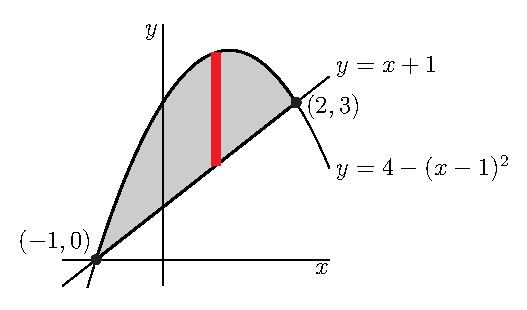
\includegraphics{OE12A_2a}
\end{center}

The red strip in the sketch above runs from $y=x+1$  to $y=4-(x-1)^2$
and so has area $[4-(x-1)^2 -(x+1)]\,\dee{x} = [2+x-x^2]\,\dee{x}$.
All together $R$ has
\begin{align*}
\text{Area}
&= \int_{-1}^2 \big[2+x-x^2\big]\ \dee{x} \\
&=\bigg[2x+\frac{x^2}{2}-\frac{x^3}{3}\bigg]_{-1}^2  \\
&=6+\frac{3}{2}-\frac{9}{3}=\frac{9}{2}
\end{align*}

\noindent (b)
We'll use vertical washers as in Example  \eref{CLP101}{eg:VOLe}
of the CLP-2 text. Note that the highest point achieved by $y=4-(x-1)^2$ is $y=4$, so rotating around the line $y=5$ causes no unexpected problems.

\begin{center}
       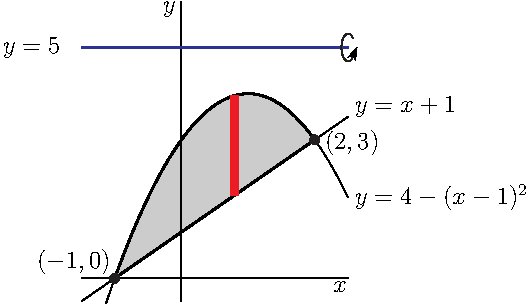
\includegraphics{OE12A_2b}
\end{center}

 \begin{itemize}
\item We cut $R$ into thin vertical strips of width $\dee{x}$ like the red
strip in the figure  above.

\item When we rotate $R$ about the horizontal line $y=5$,  each
strip  sweeps out a thin washer
\begin{itemize}
\item
whose inner radius is $r_{in}=5-[4-(x-1)^2]=1+(x-1)^2$, and
\item
whose outer radius is $r_{out}= 5-[x+1]=4-x$ and
\item
whose thickness is $\dee{x}$ and hence
\item
whose volume is
$\pi\big[r_{out}^2-r_{in}^2\big]\,\dee{x}
=\pi\big[{\big(4-x\big)}^2-{\big(1+(x-1)^2\big)}^2\big]\,\dee{x}$

\end{itemize}
\item As our leftmost strip is at $x=-1$ and our rightmost
strip is at $x=2$, the total
\begin{align*}
{\rm Volume} &= \pi\int_{-1}^2
   \big[{\big(4-x\big)}^2-{\big(1+(x-1)^2\big)}^2\big]\,\dee{x}
\end{align*}
\end{itemize}

\end{solution}
%%%%%%%%%%%%%%%%%%%


\begin{question}[M121 1999A]
 Let $\cR=\big\{(x,y)\ :\ (x-1)^2+y^2\le 1\text{
and } x^2+(y-1)^2\le 1\ \big\}$.
\begin{enumerate}[(a)]
\item
Sketch $\cR$ and find its area.
\item
 If $\cR$ rotates around the $y$--axis, what volume is generated?
\end{enumerate}
\end{question}

\begin{hint}
You can somewhat simplify your calculations in part (a) (but not part (b)) by using the fact that $\cR$ is symmetric about the line $y=x$.

When you're solving an equation for $x$, be careful about your signs: $x-1$ is negative.
\end{hint}

\begin{answer} (a)
$\dfrac{\pi}{2}-1$
\qquad(b)
$\dfrac{\pi^2}{2}-\pi\approx 1.793$
\end{answer}

\begin{solution} (a)
The curves  $(x-1)^2+y^2 = 1$ and  $x^2+(y-1)^2 = 1$
are circles of radius $1$ centered on $(1,0)$ and $(0,1)$ respectively.
Both circles pass through $(0,0)$ and $(1,1)$. They are sketched below.

\begin{center}
       \includegraphics{E121_99D_8a}
\end{center}

\noindent The region $\cR$ is symmetric about the line $y=x$, so the area
of $\cR$ is twice the area of the part of $\cR$ to the left of the line $y=x$.
The red strip in the sketch above runs from  the edge of the lower circle to $x=y$.
So, given a value of $y$ in $[0,1]$, we need to find the corresponding value of $x$ along the circle. We solve $(x-1)^2+y^2=1$ for $x$, keeping in mind that $0 \leq x\leq 1$:
\begin{align*}
(x-1)^2+y^2&=1\\
(x-1)^2&=1-y^2\\
|x-1|&=\sqrt{1-y^2}\\
1-x&=\sqrt{1-y^2}\\
x&=1-\sqrt{1-y^2}
\intertext{Now, we calculate:}
\text{Area}
&= 2\int_0^1 \big[y-\big(1-\sqrt{1-y^2}\big)\big]\ \dee{y} \\
&=2\left\{ \int_0^1 y-1\ \dee{y} + \int_0^1 \sqrt{1-y^2}\ \dee{y} \right\}\\
&=2\Big\{\Big[\frac{y^2}{2}-y\Big]_0^1 +\int_0^1\sqrt{1-y^2}\ \dee{y}\Big\} \\
&=\frac{\pi}{2}-1
\end{align*}
Here the integral  $\int_0^1\sqrt{1-y^2}\ \dee{y}$ was evaluated simply as the area
of one quarter of a cicular disk of radius $1$. It can also be evaluated by substituting
$y=\sin\theta$, a technique we'll learn more about in Section~\eref{CLP101}{sec trigsub}
of the CLP-2 text.

\noindent (b)
We'll use horizontal washers as in Example  \eref{CLP101}{eg rot yaxis}
of the %\href{http://www.math.ubc.ca/%7Efeldman/m101/clp/clp_notes_101.pdf}{CLP 101 notes}.
 in the CLP-2 text.
 \begin{itemize}
\item We cut $\cR$ into thin horizontal  strips of width $\dee{y}$ like the blue
strip in the figure  above.

\item When we rotate $\cR$ about the $y$--axis,  each strip
sweeps out a thin washer
\begin{itemize}
\item
whose inner radius is $r_{in}=1-\sqrt{1-y^2}$, and
\item
whose outer radius is $r_{out}= \sqrt{1-(y-1)^2}$ and
\item
whose thickness is $\dee{y}$ and hence
\item
whose volume is
\begin{align*}
&\pi\big[{\big(\sqrt{1-(y-1)^2}\big)}^2-{\big(1-\sqrt{1-y^2}\,\big)}^2\big]\,\dee{y}\\
=&\pi \big[  1 - (y-1)^2       -1 + 2\sqrt{1-y^2} - (1-y^2)   \big]\\
=&2\pi\big[\sqrt{1-y^2}+y-1\big]\,\dee{y}\end{align*}

\end{itemize}
\item As our bottommost strip is at $y=0$ and our topmost
strip is at $y=1$, the total
\begin{align*}
{\rm Volume} &= 2\pi\int_{0}^1\big[\sqrt{1-y^2}+y-1\big]\ \dee{y}
= 2\pi\Big[\frac{\pi}{4}+\frac{1}{2}-1\Big]\\
&=\frac{\pi^2}{2}-\pi\approx 1.793
\end{align*}
Here, we again used that $\int_{0}^1 \sqrt{1-y^2}\ dy$ is the area of a quarter
circle of radius one, and we used a calculator to approximate the final answer.
\end{itemize}

\end{solution}
%%%%%%%%%%%%%%%%%%%

\begin{Mquestion}[1997A]
Let $\cR$ be the plane region bounded by $x=0,\ x=1,\ y=0$
and $y=c\sqrt{1+x^2}$, where $c$ is a positive constant.
\begin{enumerate}[(a)]
\item
Find the volume $V_1$ of the solid obtained by revolving
$\cR$ about the $x$--axis.
\item
Find the volume $V_2$ of the solid obtained by revolving
$\cR$ about the $y$--axis.
\item
 If $V_1=V_2$, what is the value of $c$?
\end{enumerate}
\end{Mquestion}

\begin{hint}
The mechanically easiest way to answer part (b) uses the method of cylindrical
shells, which we have not covered.  The method of washers also works, but requires  you have enough patience and also
to have a good idea what $\cR$ looks like. So it is crucial to first sketch $\cR$.
Then be very careful in identifying the left end of your horizontal strips.
\end{hint}

\begin{answer} (a)
$V_1=\dfrac{4}{3}\pi c^2$
\qquad(b)
$V_2 =\dfrac{\pi\,c}{3}\big[4\sqrt{2}-2 \big] $
\qquad (c)
$c=0\text{ or }c=\sqrt{2}-\frac{1}{2}$
\end{answer}

\begin{solution}
Before we start, it will be useful to have a reasonable sketch of the graph $y=c\sqrt{1+x^2}$ over the interval $[0,1]$. Its endpoints are $(0,c)$ and $(1,c\sqrt{2})$. The function is entirely above the $x$-axis, which we need to know for part (a). For part (b), we need to know whether it is always increasing or not: when we're drawing horizontal strips, we need to know their endpoints, and if the function has ``humps," the right endpoint will not be simply the line $x=1$.

If you're comfortable noticing that $1+x^2$ increases as $x$ increases because we only consider nonnegative values of $x$, then you can also be confident that $\sqrt{1+x^2}$ is simply increasing. Alternately, we can consider the derivative:
\begin{align*}
\diff{}{x}\left\{c\sqrt{1+x^2}\right\}&=c\cdot \dfrac{1}{2\sqrt{1+x^2}}\cdot 2x = \dfrac{cx}{\sqrt{1+x^2}}
\end{align*}
Since we only consider positive values of $x$, this derivative is never negative, so the function is never decreasing. This gives us the following basic sketch:
\begin{center}
\begin{tikzpicture}
\YEaaxis{.5}{3}{.5}{3}
\YExcoord{2.5}{1}
\YEycoord{1}{c}
\draw[thick] (0,1)--(2.75,2) ;
\end{tikzpicture}
\end{center}

The figures in the solution below use a slightly more detailed rendering of our function, but so much accuracy is not necessary.

(a)
Let $\cV_1$ be the solid obtained by revolving
$\cR$ about the $x$--axis. The portion of $\cV_1$ with $x$--coordinate
between $x$ and $x+\dee{x}$ is obtained by rotating the red vertical strip in
the figure on the left below about the $x$--axis.
That portion is a disk of radius $c\sqrt{1+x^2}$ and thickness
$\dee{x}$. The volume of this disk is $\pi(c\sqrt{1+x^2})^2\dee{x}=\pi c^2 (1+x^2)\,\dee{x}$.
So the total volume of $\cV_1$ is
\begin{align*}
V_1=\int_0^1 \pi c^2 (1+x^2)\,\dee{x}
=\pi c^2\Big[x+\frac{x^3}{3}\Big]_0^1
=\frac{4}{3}\pi c^2
\end{align*}

\begin{center}
       
\includegraphics{graphE97_4l}\qquad\qquad
       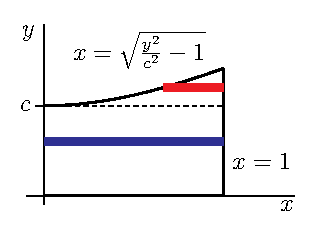
\includegraphics{graphE97_4r}
\end{center}


\noindent (b)
We'll use horizontal washers as in Example  \eref{CLP101}{eg rot yaxis}
of the %\href{http://www.math.ubc.ca/%7Efeldman/m101/clp/clp_notes_101.pdf}{CLP 101 notes}.
 in the CLP-2 text.
 \begin{itemize}
\item We cut $\cR$ into thin horizontal  strips of width $\dee{y}$ as in
the figure on the right above.

\item When we rotate $\cR$ about the $y$--axis, i.e. about the line $x=0$, each strip
sweeps out a thin washer
\begin{itemize}
\item
whose outer radius is $r_{out}=1$, and
\item
whose inner radius is $r_{in}= \sqrt{\frac{y^2}{c^2}-1}$ when $y\ge c\sqrt{1+0^2}=c$
(see the red strip in the figure on the right above),  and
whose inner radius is $r_{in}= 0$ when $y\le c$
(see the blue strip in the figure on the right above) and
\item
whose thickness is $\dee{y}$ and hence
\item
whose volume is
$\pi(r_{out}^2 - r_{in}^2)\dee{y} = \pi\big(2-\frac{y^2}{c^2}\big)\dee{y}$
when $y\ge c$ and  whose volume is
$\pi(r_{out}^2 - r_{in}^2)\dee{y} = \pi\,\dee{y}$
when $y\le c$ and

\end{itemize}
\item As our bottommost strip is at $y=0$ and our topmost
strip is at $y=\sqrt{2}\,c$ (since at the top $x=1$ and $y= c\sqrt{1+x^2}$), the total
\begin{align*}
V_2
&= \int _c^{\sqrt{2}\,c}  \pi\Big(2-\frac{y^2}{c^2}\Big)\dee{y}
+\int _ 0^c \pi\,\dee{y} \\
&=\pi{\Big[2y -\frac{y^3}{3c^2}\Big]}_c^{\sqrt{2}\,c} +\pi c\\
&=\pi\,c\Big[\frac{4\sqrt{2}}{3}-\frac{5}{3} \Big]+\pi c \\[0.05in]
&=\frac{\pi\,c}{3}\big[4\sqrt{2}-2 \big]
\end{align*}
\end{itemize}

\noindent (c)
We have $V_1=V_2$ if and only if
\begin{align*}
\frac{4}{3}\pi c^2&=\frac{\pi\,c}{3}\big[4\sqrt{2}-2 \big]  \\
4c^2&=c\left(4\sqrt{2}-2\right)\\
4c^2-c\left(4\sqrt{2}-2\right)&=0\\
4c\left(c - \left(\sqrt{2}-\frac{1}{2}\right)\right)&=0\\
c=0 \quad\mbox{or}\quad c&=\sqrt{2}-\frac{1}{2}
\end{align*}


\end{solution}
%%%%%%%%%%%%%%%%%%%

\begin{question}[2013A]
The graph below shows the region between
$y = 4 + \pi \sin x$ and $y = 4 + 2\pi - 2x$.

\begin{center}
       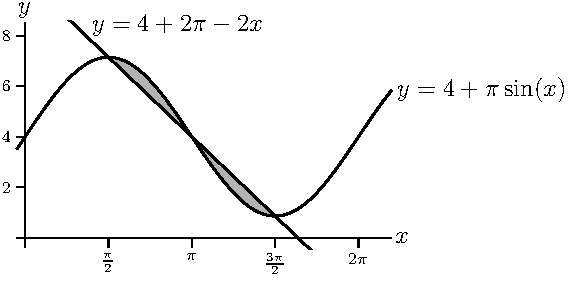
\includegraphics{OE13A_4a}
\end{center}

\noindent The region is rotated about the line $y = -1$.
Express in terms of definite integrals the volume of the resulting
solid. Do not evaluate the integrals.
\end{question}

\begin{hint}
Note that the curves cross. The area of this
region was found in Problem \ref{prob_s1.5q5} of Section 1.5.
It would be useful to review that problem.
\end{hint}

\begin{answer}
$\displaystyle\int_{\pi/2}^\pi \pi\big[(5 + \pi \sin x)^2-(5 + 2\pi - 2x)^2\big]\ \dee{x}
   +\displaystyle\int^{3\pi/2}_\pi \pi\big[(5 + 2\pi - 2x)^2-(5 + \pi \sin x)^2\big]\
            \dee{x}$
\end{answer}

\begin{solution}
We will compute the volume by rotating thin vertical strips as in
the sketch

\begin{center}
       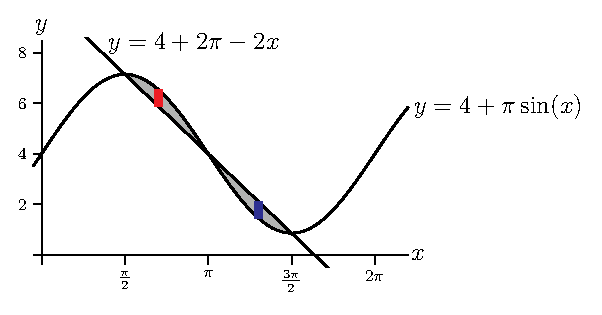
\includegraphics{OE13A_4}
\end{center}

\noindent
about the line $y=-1$ to generate thin washers.
We need to know when the line $y = 4 + 2\pi - 2x$ intersects the curve
$y = 4 + \pi \sin x$. Looking at the graph, it appears to be at $\frac{\pi}{2}$, $\pi$, and $\frac{3\pi}{2}$. By plugging in these values of $x$ to both functions, we see they are indeed the points of intersection.

\begin{itemize}
\item
When $\frac{\pi}{2} \le x \le \pi$, the top of the strip is at
$y = 4 + \pi \sin x$ and the bottom of the strip is at $y = 4 + 2\pi - 2x$.
When the strip is rotated, we get a thin washer with
outer radius $R_1(x)= 1+ 4 + \pi \sin x=5 + \pi \sin x $ and inner radius
$r_1(x) = 1+4 + 2\pi - 2x=5 + 2\pi - 2x$.
\item
When $\pi \le x \le \frac{3\pi}{2}$, the top of the strip is at
$y = 4 + 2\pi - 2x$ and the bottom of the strip is at $y = 4 + \pi \sin x$.
When the strip is rotated, we get a thin washer with outer radius
$R_2(x) = 1+4 + 2\pi - 2x=5 + 2\pi - 2x$ and inner radius
$r_2(x) = 1+ 4 + \pi \sin x=5 + \pi \sin x$.

\end{itemize}
So, the total
\begin{align*}
\hbox{Volume}
&= \int_{\pi/2}^\pi \pi\big[R_1(x)^2-r_1(x)^2\big]\ \dee{x}
   +\int^{3\pi/2}_\pi \pi\big[R_2(x)^2-r_2(x)^2\big]\ \dee{x}\\
&= \int_{\pi/2}^\pi \pi\big[(5 + \pi \sin x)^2-(5 + 2\pi - 2x)^2\big]\ \dee{x}
    \\ &\hskip0.5in
   +\int^{3\pi/2}_\pi \pi\big[(5 + 2\pi - 2x)^2-(5 + \pi \sin x)^2\big]\
            \dee{x}
\end{align*}
\end{solution}
%%%%%%%%%%%%%%%%%%%
\begin{Mquestion}\label{prob_s1.6:density}
%A rod with a circular cross section is one metre long, and has a constant diameter of
%10cm.
%It is manufactured so that, $x$ centimetres from one end, the density of the material is $ x~ \frac{\mathrm{g}}{{\mathrm{cm}^3}}$. What is the weight of the entire rod?

On a particular, highly homogeneous\footnote{This is clearly a simplified model: air density changes all the time, and depends on lots of complicated factors aside from altitude. However, the equation we're using is not so far off from an idealized model of the earth's atmosphere, taken from \emph{Pressure and the Gas Laws} by H.P. Schmid, \url{http://www.indiana.edu/~geog109/topics/10_Forces&Winds/GasPressWeb/PressGasLaws.html}, accessed 3 July 2017.} planet, we observe that the density of the atmosphere $h$ kilometres above the surface is given by the equation $\rho(h) = c2^{-h/6}\quad \frac{\mathrm{kg}}{\mathrm{m^3}}$, where $c$ is the density on the planet's surface.
\begin{enumerate}[(a)]
\item What is the mass of the atmosphere contained in a vertical column with radius one metre,  sixty kilometres high?
\item What height should a column be to contain $\dfrac{3000c\pi}{\log 2}$ kilograms of air?
\end{enumerate}
\end{Mquestion}
\begin{hint}
You can use ideas from this section to answer the question. If you take a very thin slice of the column, the density is almost constant, so you can find the mass. Then you can add up all your little slices. It's the same idea as volume, only applied to mass.

Do be careful about units: in the problem statement, some are given in metres, others in kilometres.

If you're having a hard time with the antiderivative, try writing the exponential function with base $e$. Remember $2 = e^{\log 2}$.
\end{hint}
\begin{answer}
(a) $\dfrac{6000c\pi}{\log 2}\left(1-\dfrac{1}{2^{10}}\right)$, which is close to
$\dfrac{6000c\pi}{\log 2}$.

(b) 6km: that is, there is roughly the same mass of air in the lowest 6 km of the column as there is in the remaining 54 km.
\end{answer}
\begin{solution}
(a)

We use the same ideas for volume, and apply them to mass. We want to take slices of the column, approximate their mass, then add them up. To reconcile our units, let $k=1000h$, so $k$ is the height in metres. Then the density of air at height $k$ is $c2^{-k/6000} ~\frac{\mathrm{kg}}{\mathrm{m}^3}$.

A horizontal slice of the column is a circular disk with height $\dee{k}$ and radius $1$ m. So, its volume is $\pi~ \dee{k}~\mathrm{m^3}$. What we're interested in, though, is its mass. At height $k$, its mass is
\begin{align*}
(\mathrm{volume})\times (\mathrm{density})&=\left(\pi ~\dee{k} ~\mathrm{m^3}\right)\times \left(c2^{-k/6000}~\frac{\mathrm{kg}}{\mathrm{m^3}}\right)\\
&=c\pi2^{-k/6000}~\dee{k}\quad\mathrm{kg}
\intertext{Since $k$ runs from 0 to $60,000$, the total mass is given by}
\int_0^{60000} c\pi2^{-k/6000}~\dee{k}&=c\pi\int_0^{60000} 2^{-k/6000}~\dee{k}
\intertext{To facilitate integration, we can write our exponential function in terms of $e$, then use the substitution $u=-\frac{k}{6000}\log 2$, $\dee{u} = -\frac{1}{6000}\log 2~\dee{k}$.}
&=c\pi\int_0^{60000}\left(e^{\log 2}\right)^{-k/6000}\dee{k}\\
&=c\pi\int_0^{60000}e^{-\tfrac{k}{6000}\log 2}\dee{k}\\
&=-\frac{6000c\pi}{\log 2}\int_0^{-10\log 2}e^{u}\dee{u}\\
&=\frac{6000c\pi}{\log 2}\int_{-10\log 2}^0e^{u}\dee{u}\\
&=\frac{6000c\pi}{\log 2}\left(1-\frac{1}{2^{10}}\right)
\end{align*}
We note this is fairly close to $\dfrac{6000c\pi}{\log 2}$.

We also remark that this is a demonstration of the usefulness of integrals. We wanted to know how much of \emph{something} there was, but the amount of that something was different everywhere: more in some places, less in others. Integration allowed us to account for this gradient. You've seen this behaviour exploited to find distances travelled, areas, volumes, and now mass. In your studies, you will doubtless learn to use it to find still more  quantities, and we will discuss other applications in Chapter~\eref{CLP101}{chap int app} of the CLP-2 text.

(b) We want to find the value of $k$ that gives a mass of $\dfrac{3000c\pi}{\log 2}$. By following our reasoning above, the mass of air in the column from the ground to height $k$ is
\begin{align*}
\frac{6000c\pi}{\log 2}\left(1-\frac{1}{2^{k/6000}}\right)&
\intertext{So, we set this equal to the mass we want, and solve for $k$.}
\frac{6000c\pi}{\log 2}\left(1-\frac{1}{2^{k/6000}}\right)&=\frac{3000c\pi}{\log 2}\\
2\left(1-\frac{1}{2^{k/6000}}\right)&=1\\
1&=\frac{2}{2^{k/6000}}\\
2^{k/6000}&=2^1\\
k&=6000\\
h&=6
\end{align*}

This means that there is roughly the same mass of air in the lowest 6 km of the column as there is in the remaining 54 km.
\end{solution}

%%%%%%%%%%%%%%%%%%%%
%
%\begin{question}
%A right circular cone with base radius $r$ and height $h$ is sliced vertically, as shown in the picture below. The cut is made so that the slice makes a chord across the circle sweeping out an angle of $\frac{\pi}{2}$ radians.
% Find the volume of the red piece.
%\begin{center}
%\hfill
%\begin{tikzpicture}
%\draw (0,0)node[shape=ellipse, minimum width=3cm, minimum height=1cm, draw] {};
%\draw (-1.5,0)--(0,3)--(1.5,0);
%\draw[dashed] (0,0)--(0,3) node[midway, left]{$h$};
%\draw[dashed] (0,0)--(-1.5,0) node[midway, below]{$r$};
%\draw[thick, fill=red, fill opacity=0.1] (-60:1.5cm and .5cm) arc (-60:60:1.5cm and .5cm) ;
%\filldraw[red, thick, left color=red!70!black, right color=white, fill, fill opacity=0.2] (.75,1.5)--(.75,-.4)arc (-60:0:1.5cm and .5cm) --cycle;
%\draw (0,-1) node{sliced cone};
%\end{tikzpicture}
%\hfill\begin{tikzpicture}
%\draw (0,0) node[shape=circle, minimum size=3cm, draw]{};
%\draw[dashed] (0,0)--(-1.5,0) node[below, midway]{$r$};
%\draw[red, fill=red, fill opacity=0.2] (0,0) + (45:1.5cm) arc (45:-45:1.5cm)--cycle;
%\draw (0,-2.) node{sliced base};
%\draw[dashed] (1.06,1.06)--(0,0)--(1.06,-1.06);
%\draw (.35,.35) arc(45:-45:.5cm) node[above right]{$\frac{\pi}{2}$};
%\end{tikzpicture}
%\hfill~
%\end{center}
%\end{question}
%\begin{hint}
%You'll want to use horizontal cross sections, like Example~\eref{CLP101}{eg:VOLa} of the
%CLP-2 text. Then the area of your slice can be calculated as a section of a circle, minus a triangle.
%\end{hint}
%\begin{answer}
%$ \dfrac{r^2h}{3}\left(\dfrac{\pi}{4}-\dfrac{1}{2}\right)$
%\end{answer}
%\begin{solution}
%As in Example~\eref{CLP101}{eg:VOLa} of the CLP-2 text, we take horizontal slices. If the radius of a slice is $s$, then its area can be calculated as one-quarter of the circle of radius $s$, minus the right triangle with base and height both $s$. So, \[A = \frac{1}{4}\left(\pi s^2\right) - \frac{1}{2} s^2 = s^2\left(\frac{\pi}{4}-\frac{1}{2}\right).\]
%
%As we climb up the cone, the radius of our slices changes. As in the text, let's assume that the base of the cone sits at $y=h$, and the tip is at $y=0$. Then we use similar triangles to conclude that at height $y$, the radius of the cone is $s=\left(\frac{r}{h}\right)y$.
%
%\begin{center}
%\begin{tikzpicture}
%\YEaaxis{1}{4}{1}{5}
%\YEycoord{2}{y}
%\YEycoord{4}{h}
%\YExcoord{3}{r}
%\draw (0,0)--(3,4)--(0,4);
%\fill[fill opacity=0.1] (0,0)--(1.5,2)--(0,2)--cycle;
%\draw (0,2)--(1.5,2);
%\draw (.75,2.25) node{$s$};
%\draw (5,3) node{$\dfrac{s}{y}=\dfrac{r}{h}$};
%\end{tikzpicture}
%\end{center}
%
%So:
%\begin{itemize}
%\item Our slices run from $y=0$ to $y=h$,
%\item at height $y$, the area of our slice is $\left(\frac{r}{h}\cdot y\right)^2\left(\frac{\pi}{4}-\frac{1}{2}\right) = y^2\left(\frac{r}{h}\right)^2\left(\frac{\pi}{4}-\frac{1}{2}\right)$,
%\item and the height of our slice is $\dee{y}$.
%\end{itemize}
%\item So, the volume of our piece of cone is:
%
%\begin{align*}
%\mbox{Volume}&=\int_0^h y^2\left(\frac{r}{h}\right)^2\left(\frac{\pi}{4}-\frac{1}{2}\right)\ \dee{y}\\
%&=\left(\frac{r}{h}\right)^2\left(\frac{\pi}{4}-\frac{1}{2}\right)\int_0^h y^2\ \dee{y}
%\\&=
%\left(\frac{r}{h}\right)^2\left(\frac{\pi}{4}-\frac{1}{2}\right)\frac{1}{3}h^3\\
%&= \frac{r^2h}{3}\left(\frac{\pi}{4}-\frac{1}{2}\right)
%\end{align*}
%\end{solution}


%%%%%%%%%%%%%%%%%%%%%%%%%%%%%%%%%%%%%

\section{Integration by parts}
%
% Copyright 2018 Joel Feldman, Andrew Rechnitzer and Elyse Yeager.
% This work is licensed under a Creative Commons Attribution-NonCommercial-ShareAlike 4.0 International License.
% https://creativecommons.org/licenses/by-nc-sa/4.0/
%
\questionheader{ex:s1.7}

%%%%%%%%%%%%%%%%%%
\subsection*{\Conceptual}
%%%%%%%%%%%%%%%%%%
\begin{Mquestion}\label{1.7_difftoint}
The method of integration by substitution comes from the $\rule{1.5cm}{0.15mm}$ rule for differentiation.\\
The method of integration by parts comes from the  $\rule{1.5cm}{0.15mm}$ rule for differentiation.
\end{Mquestion}
\begin{hint}
Read back over Sections~\eref{CLP101}{sec subs} and \eref{CLP101}{sec intbyparts}
of the CLP--II text. When these methods are introduced, they are justified using the
corresponding differentiation rules.
\end{hint}
\begin{answer}
chain; product
\end{answer}
\begin{solution}
Integration by substitution is just using the chain rule, backwards:
\begin{alignat*}{3}
&&\diff{}{x}\{f(g(x))\}&=f'(g(x))g'(x)\\
&\Leftrightarrow& \int\diff{}{x}\{f(g(x))\}\dee{x}+C&=\int f'(g(x))g'(x)\dee{x}\\
&\Leftrightarrow&\underbrace{ f(g(x))}_{f(u)} +C &=\int \underbrace{f'(g(x))}_{f'(u)}\underbrace{g'(x)\dee{x}}_{\dee{u}}
\intertext{Similarly, integration by parts comes from the product rule:}
&&\diff{}{x}\{f(x)g(x)\}&=f'(x)g(x)+f(x)g'(x)\\
&\Leftrightarrow&\int\diff{}{x}\{f(x)g(x)\}\dee{x}+C&=\int f'(x)g(x)+f(x)g'(x)\dee{x}\\
&\Leftrightarrow&f(x)g(x)+C&=\int f'(x)g(x)\dee{x}+\int f(x)g'(x)\dee{x}\\
&\Leftrightarrow&\int\underbrace{ f(x)}_{u}\underbrace{g'(x)\dee{x}}_{\dee{v}}&=\underbrace{f(x)}_{u}\underbrace{g(x)}_{v}-\int \underbrace{g(x)}_{v}\underbrace{f'(x)\dee{x}}_{\dee{u}}\\
\end{alignat*}
\end{solution}
%%%%%%%%%%%%%%%%%%%

\begin{question}
Suppose you want to evaluate an integral using integration by parts. You choose part of your integrand to be $u$, and part to be $\dee{v}$. The part chosen as $u$ will be: (differentiated, antidifferentiated). The part chosen as $\dee{v}$ will be: (differentiated, antidifferentiated).
\end{question}
\begin{hint}
Remember our rule: $\int u \dee{v} = uv - \int v \dee{u}$. So, we take $u$ and use it to make $\dee{u}$, and we take $\dee{v}$ and use it to make $v$.
\end{hint}
\begin{answer}
The part chosen as $u$ will be differentiated. The part chosen as $\dee{v}$ will be antidifferentiated.
\end{answer}
\begin{solution}
Remember our rule: $\int u \dee{v} = uv - \int v \dee{u}$. So, we take $u$ and use it to make $\dee{u}$--that is, we differentiate it. We take $\dee{v}$ and use it to make $v$--that is, we antidifferentiate it.
\end{solution}


%%%%%%%%%%%%%%%%%%%
\begin{question}
Let $f(x)$ and $g(x)$ be differentiable functions. Using the quotient rule for differentiation, give an equivalent expression to $\displaystyle\int \frac{f'(x)}{g(x)}~\dee{x}$.
\end{question}
\begin{hint}
According to the quotient rule,
\[\diff{}{x}\left\{\dfrac{f(x)}{g(x)}\right\} = \frac{g(x)f'(x)-f(x)g'(x)}{g^2(x)}.\]
Antidifferentiate both sides of the equation, then solve for the expression in the question.
\end{hint}
\begin{answer}
$\displaystyle\int \frac{f'(x)}{g(x)}~\dee{x}= \dfrac{f(x)}{g(x)} +\displaystyle\int\frac{f(x)g'(x)}{g^2(x)}\dee{x}+C$
\end{answer}
\begin{solution}
We'll use the same ideas that lead to the methods of substitution and integration by parts. (You can review these in your text, or see the solution to Question~\ref{1.7_difftoint} in this section.)
According to the quotient rule,
\begin{align*}
\diff{}{x}\left\{\dfrac{f(x)}{g(x)}\right\} &= \frac{g(x)f'(x)-f(x)g'(x)}{g^2(x)}.
\intertext{Antidifferentiating both sides gives us:}
\int\diff{}{x}\left\{\dfrac{f(x)}{g(x)}\right\} \dee{x}+C&= \int\frac{g(x)f'(x)-f(x)g'(x)}{g^2(x)}\dee{x}\\
\dfrac{f(x)}{g(x)} +C&= \int\frac{f'(x)}{g(x)}\dee{x}-\int\frac{f(x)g'(x)}{g^2(x)}\dee{x}
\\\int\frac{f'(x)}{g(x)}\dee{x}
&= \dfrac{f(x)}{g(x)}+\int\frac{f(x)g'(x)}{g^2(x)}\dee{x}+C
\end{align*}

This isn't quite at catchy as integration by parts--which is probably why it hasn't caught on as a rule with its own name.
\end{solution}

%%%%%%%%%%%%%%%%%%%

\begin{Mquestion}
Suppose we want to use integration by parts to evaluate $\displaystyle\int u(x)\cdot v'(x) \dee{x}$ for some differentiable functions $u$ and $v$. We need to find an antiderivative of $v'(x)$, but there are infinitely many choices. Show that every antiderivative of $v'(x)$ gives an equivalent final answer.
\end{Mquestion}
\begin{hint}
Remember all the antiderivatives differ only by a constant, so you can write them all as $v(x)+C$ for some $C$.
\end{hint}
\begin{answer}
All the antiderivatives differ only by a constant, so we can write them all as $v(x)+C$ for some $C$. Then, using the formula for integration by parts,
\begin{align*}
\int u(x)\cdot v'(x) \dee{x}&=\underbrace{u(x)}_u\underbrace{\big[ v(x)+C\big]}_v - \int \underbrace{\big[ v(x)+C\big]}_v \underbrace{u'(x)\dee{x}}_{\dee{u}}\\
&=u(x)v(x)+Cu(x) - \int v(x)u'(x)\dee{x} - \int Cu'(x)\dee{x}
\\&=u(x)v(x)+Cu(x) - \int v(x)u'(x)\dee{x} - Cu(x)+D
\\&=u(x)v(x) - \int v(x)u'(x)\dee{x} +D
\end{align*}
where $D$ is any constant.

Since the terms with $C$ cancel out, it didn't matter what we chose for $C$--all choices end up the same.
\end{answer}
\begin{solution}
All the antiderivatives differ only by a constant, so we can write them all as $v(x)+C$ for some $C$. Then, using the formula for integration by parts,
\begin{align*}
\int u(x)\cdot v'(x) \dee{x}&=\underbrace{u(x)}_u\underbrace{\big[ v(x)+C\big]}_v - \int \underbrace{\big[ v(x)+C\big]}_v \underbrace{u'(x)\dee{x}}_{\dee{u}}\\
&=u(x)v(x)+Cu(x) - \int v(x)u'(x)\dee{x} - \int Cu'(x)\dee{x}
\\&=u(x)v(x)+Cu(x) - \int v(x)u'(x)\dee{x} - Cu(x)+D
\\&=u(x)v(x) - \int v(x)u'(x)\dee{x} +D
\end{align*}
where $D$ is any constant.

Since the terms with $C$ cancel out, it didn't matter what we chose for $C$--all choices end up the same.
\end{solution}
%%%%%%%%%%%%%%%%%%%


\begin{question}\label{1.7_badchoices}
Suppose you want to evaluate $\displaystyle\int f(x)\dee{x}$ using integration by parts. Explain why $\dee{v} = f(x)\dee{x}$, $u=1$ is generally a bad choice.

Note: compare this to Example~\eref{CLP101}{eg:PRTSlnx} of the CLP--II text, where we chose $u=f(x)$, $\dee{v}=1\dee{x}$.
\end{question}
\begin{hint}
What integral do you have to evaluate, after you plug in your choices to the integration by parts formula?
\end{hint}
\begin{answer}
Suppose we choose $\dee{v} = f(x)\dee{x}$, $u=1$. Then $v = \displaystyle\int f(x)\dee{x}$, and $\dee{u}=\dee{x}$. So, our integral becomes:
\begin{align*}
\int \underbrace{(1)}_{u}\underbrace{f(x)\dee{x}}_{\dee{v}}&=
\underbrace{(1)}_{u}\underbrace{\int f(x)\dee{x}}_{v} - \int\underbrace{ \left(\int f(x)\dee{x}\right)}_{v}\underbrace{\dee{x}}_{\dee{u}}
\end{align*}
In order to figure out the first product (and the second integrand), you need to know the antiderivative of $f(x)$--but that's exactly what you're trying to figure out!
\end{answer}
\begin{solution}
Suppose we choose $\dee{v} = f(x)\dee{x}$, $u=1$. Then $v = \displaystyle\int f(x)\dee{x}$, and $\dee{u}=\dee{x}$. So, our integral becomes:
\begin{align*}
\int \underbrace{(1)}_{u}\underbrace{f(x)\dee{x}}_{\dee{v}}&=
\underbrace{(1)}_{u}\underbrace{\int f(x)\dee{x}}_{v} - \int\underbrace{ \left(\int f(x)\dee{x}\right)}_{v}\underbrace{\dee{x}}_{\dee{u}}
\end{align*}
In order to figure out the first product (and the second integrand), you need to know the antiderivative of $f(x)$--but that's exactly what you're trying to figure out! So, using integration by parts has not eased your pain.

We note here that in certain cases, such as $\int\log x~ \dee{x}$ (Example~\eref{CLP101}{eg:PRTSlnx}  in the CLP--II text), it is useful to choose $\dee{v}=1\dee{x}$. This is similar to, but crucially different from, the do-nothing method in this problem.
\end{solution}



%%%%%%%%%%%%%%%%%%
\subsection*{\Procedural}
%%%%%%%%%%%%%%%%%%

\begin{Mquestion}[M121 2014A]\label{1.7_xlogx}
Evaluate ${\displaystyle\int x\log x\,\dee{x}}$.
\end{Mquestion}

\begin{hint}
You'll probably want to use integration by parts. (It's the title of the section, after all). You'll break the integrand into two parts, integrate one, and differentiate the other. Would you rather integrate $\log x$, or differentiate it?
\end{hint}

\begin{answer}
$\dfrac{x^2\log x}{2} - \dfrac{x^2}{4} + C$
\end{answer}

\begin{solution}
For integration by parts, we want to break the integrand into two pieces, multiplied together. There is an obvious choice for how to do this: one piece is $x$, and the other is $\log x$. Remember that one piece will be integrated, while the other is differentiated. The question is, which choice will be more helpful. After some practice, you'll get the hang of making the choice. For now, we'll present both choices--but when you're writing a solution, you don't have to write this part down. It's enough to present your choice, and then a successful computation is justification enough.

\IBP{x}{x}{1}{\dfrac{1}{2}x^2}{\log x}{\dfrac{1}{x}}{??}

In Example~\eref{CLP101}{eg:PRTSlnx} of the CLP--II text, we found the antiderivative of logarithm, but it wasn't trivial. We might reasonably want to avoid using this complicated antiderivative. Indeed,  Option 2 (differentiating logarithm, antidifferentiating $x$) looks promising--when we multiply the blue equations, we get something easily integrable-- so let's not even bother going deeper into Option 1.

That is, we perform integration by parts with $u=\log x$ and $\dee{v}=x\,\dee{x}$,
so that $\dee{u}=\frac{\dee{x}}{x}$ and $v = \frac{x^2}{2}$.
\begin{align*}
\int\underbrace{ x}_{u}\underbrace{\log x\,\dee{x}}_{\dee{v}}
   &= \underbrace{\frac{x^2\log x}{2}}_{uv} - \int \underbrace{\frac{x^2}{2}}_v\ \underbrace{\frac{\dee{x}}{x}}_{\dee{u}}
    = \frac{x^2\log x}{2} -\frac{1}{2} \int x \ \dee{x} \\
   &= \frac{x^2\log x}{2} - \frac{x^2}{4} + C
\end{align*}
\end{solution}
%%%%%%%%%%%%%%%%%%%

\begin{question}[M105 2013A]\label{1.7_xlogx2}
Evaluate ${\displaystyle\int \frac{\log x}{x^7}\,\dee{x}}$.
\end{question}

\begin{hint}
This problem is similar to Question~\ref{1.7_xlogx}.
\end{hint}

\begin{answer}
$- \dfrac{\log x}{6 x^6} - \dfrac{1}{36 x^6} + C$
\end{answer}

\begin{solution}
Our integrand is the product of two functions, and there's no clear substitution. So, we might reasonably want to try integration by parts. Again, we have two obvious pieces: $\log x$, and $x^{-7}$. We'll consider our options for assigning these to $u$ and $\dee{v}$:

\IBP{x}{\log x}{\dfrac{1}{x}}{??}{x^{-7}}{-7x^{-8}}{\dfrac{1}{-6}x^{-6}}

Again, we remember that logarithm has some antiderivative we found in Example~\eref{CLP101}{eg:PRTSlnx} of the CLP--II text, but it was something complicated. Luckily, we don't need to bother with it: when we multiply the red equations in Option 1, we get a perfectly workable integral.

We perform integration by parts with $u=\log x$ and $\dee{v}=x^{-7}\,\dee{x}$,
so that $\dee{u}=\frac{\dee{x}}{x}$ and $v = -\frac{x^{-6}}{6}$.
\begin{align*}
\int \frac{\log x}{x^7}\,\dee{x}
   &=\underbrace{ -\log x\ \frac{x^{-6}}{6}}_{uv} + \int \underbrace{\frac{x^{-6}}{6}}_{-v}\ \underbrace{\frac{\dee{x}}{x}}_{du}
    = - \frac{\log x}{6 x^6} +\frac{1}{6} \int x^{-7} \ \dee{x} \\
   &= - \frac{\log x}{6 x^6} - \frac{1}{36 x^6} + C
\end{align*}
\end{solution}
%%%%%%%%%%%%%%%%%%%

\begin{Mquestion}[2016A]\label{1.7_xsinx}
Evaluate $\displaystyle\int_0^\pi x\sin x\,\dee{x}$.
\end{Mquestion}

\begin{hint}
 Example \eref{CLP101}{eg:PRTSxsinx} in the
%\href{http://www.math.ubc.ca/%7Efeldman/m101/clp/clp_notes_101.pdf}{CLP 101 notes}.
CLP--II text shows you how to find the antiderivative. Then the Fundamental Theorem of Calculus Part 2 gives you the definite integral.
\end{hint}

\begin{answer}
$\pi$
\end{answer}

\begin{solution}
To integrate by parts, we need to decide what to use as $u$, and what to use as $\dee{v}$. The salient parts of this integrand are $x$ and $\sin x$, so we only need to decide which is $u$ and which $\dee{v}$. Again, this process will soon become familiar, but to help you along we show you both options below.

\IBP{x}{x}{1}{\dfrac{1}{2}x^2}{\sin x}{\cos x}{-\cos x}

The derivative and antiderivative of sine are almost the same, but $x$ turns into something simpler when we differentiate it. So, we choose Option 1.

We integrate by parts, using $u = x$, $\dee{v} =\sin x \,\dee{x}$
so that $v=-\cos x$ and $\dee{u} = \dee{x}$:
\begin{align*}
\int_0^\pi x\sin x\,\dee{x}
   = \underbrace{-x\cos x}_{uv} \Big|_0^\pi -\int_0^\pi \underbrace{(-\cos x)}_v\,\underbrace{\dee{x}}_{\dee{u}}
   = \Big[-x\cos x +\sin x\Big]_0^\pi
   =-\pi(-1)
   =\pi
\end{align*}
\end{solution}
%%%%%%%%%%%%%%%%%%%

\begin{question}[M105 2015A]
Evaluate $\displaystyle\int_0^{\frac{\pi}{2}} x\cos x\,\dee{x}$.
\end{question}

\begin{hint}
Compare to Question~\ref{1.7_xsinx}. Try to do this one all the way through without peeking at another solution!
\end{hint}

\begin{answer}
$\dfrac{\pi}{2} -1$
\end{answer}

\begin{solution}
When we have two functions multiplied like this, and there's no obvious substitution, our minds turn to integration by parts. We hope that our integral will be improved by differentiating one part and antidifferentiating the other. Let's see what our choices are:

\IBP{x}{x}{1}{\dfrac{1}{2}x^2}{\cos x}{-\sin x}{\sin x}

Option 1 seems preferable. We integrate by parts, using $u = x$, $\dee{v} =\cos x \,\dee{x}$
so that $v=\sin x$ and $\dee{u} = \dee{x}$:
\begin{align*}
\int_0^{\frac{\pi}{2}} x\cos x\,\dee{x}
   = \underbrace{x}_u\underbrace{\sin x}_v \Big|_0^{\frac{\pi}{2}} -\int_0^{\frac{\pi}{2}} \underbrace{\sin x}_v\,\underbrace{\dee{x}}_{\dee{u}}
   = \Big[x\sin x +\cos x\Big]_0^{\frac{\pi}{2}}
   =\frac{\pi}{2} - 1
\end{align*}
\end{solution}
%%%%%%%%%%%%%%%%%%%

\begin{question}\label{1.7_repeated} Evaluate
$\displaystyle\int_0^1 x^3 e^x \dee{x}$.
\end{question}
\begin{hint}
If at first you don't succeed, try using integration by parts a few times in a row. Eventually, one part will go away.
\end{hint}
\begin{answer}
$e^x\left(x^3-3x^2+6x - 6\right)+C$
\end{answer}
\begin{solution}
This integrand is the product of two functions, with no obvious substitution. So, let's try integration by parts, with one part $e^x$ and one part $x^3$.

\IBP{x}{e^x}{e^x}{e^x}{x^3}{3x^2}{\frac{1}{4}x^4}

At first glance, multiplying the red functions and multiplying the blue functions give largely equivalent integrands to what we started with--none of them with obvious antiderivatives. In previous questions, we were able to choose $u=x$, and then $\dee{u}=\dee{x}$, so the ``$x$" in  the integrand effectively went away. Here, we see that choosing $u=x^3$ will lead to $\dee{u}=3x^2\dee{x}$, which has a lower power. If we repeatedly perform integration by parts, choosing $u$ to be the power of $x$ each time, then after a few iterations it should go away, because the third derivative of $x^3$ is a constant.

So, we start with Option 2: $u=x^3$, $\dee{v}=e^x\dee{x}$, $\dee{u}=3x^2\dee{x}$, and $v = e^x$.

\begin{align*}
\int x^3 e^x \dee{x}&= \underbrace{x^3}_{u}\underbrace{e^x}_{v} - \int
\underbrace{e^x}_v \cdot\underbrace{ 3x^2 \dee{x}}_{\dee{u}}\\
&= {x^3}{e^x} -3 \int
{e^x} \cdot x^2 \dee{x}
\intertext{Now, we take $u=x^2$ and $\dee{v}=e^x\dee{x}$, so $\dee{u}=2x\dee{x}$ and $v=e^x$. We're only using integration by parts on the actual integral--the rest of the function stays the way it is.}
&=x^3e^x -3
 \left[\underbrace{x^2e^x}_{uv} - \int \underbrace{e^x}_{v} \cdot \underbrace{2x\dee{x}}_{\dee{u}}\right]
\\
&=x^3e^x - 3x^2e^x + 6\int x e^x\dee{x}
\intertext{Continuing, we take $u=x$ and $\dee{v}=e^x\dee{x}$, so $\dee{u}=\dee{x}$ and $v=e^x$. This is the step where the polynomial part of the integrand finally disappears.}
&=x^3e^x - 3x^2e^x +
6\left[\underbrace{xe^x}_{uv} - \int \underbrace{ e^x}_v \underbrace{\dee{x}}_{\dee{u}}\right]\\
 &=x^3e^x-3x^2e^x+6xe^x - 6e^x+C
\\ &=e^x\left(x^3-3x^2+6x - 6\right)+C
\end{align*}

Let's check that this makes sense: the derivative of $e^x\left(x^3-3x^2+6x - 6\right)+C$ should be $x^3e^x$. We differentiate using the product rule.
\begin{align*}
\diff{}{x}\left\{e^x\left(x^3-3x^2+6x - 6\right)+C\right\}
&=e^x\left(x^3-3x^2+6x - 6\right)+e^x\left(3x^2-6x+6\right)\\
&=e^x\left(x^3-3x^2+3x^2+6x-6x-6+6\right)=x^3e^x
\end{align*}

Remark: In order to be technically correct in our antidifferentiation, we should add the $+C$ as soon as we do the first integration by parts. However, when we are using integration by parts, we usually end up evaluating an integral at the end, and we add the $+C$ at that point. Since the $+C$ comes up eventually, it is common practice to not clutter our calculations with it until the end.
\end{solution}
%%%%%%%%%%%%%%%%%%%
\begin{question}
Evaluate $\displaystyle\int x \log^3 x~ \dee{x}$.
\end{question}
\begin{hint}
Similarly to Question~\ref{1.7_repeated}, look for a way to use integration by parts a few times to simplify the integrand until it is antidifferentiatable.
\end{hint}
\begin{answer}
$\dfrac{x^2}{2}\log^3x -
\dfrac{3x^2}{4}\log^2 x + \dfrac{3x^2}{4}\log x
 - \dfrac{3x^2}{8}+C$
\end{answer}
\begin{solution}
Since our integrand is two functions multiplied together, and there isn't an obvious substitution, let's try integration by parts. Here are our salient options.

\IBP{x}{x}{1}{\dfrac{1}{2}x^2}{\log^3 x}{3\log^2 x \cdot\frac{1}{x}}{??}

This calls for some strategizing. Using the template of Example~\eref{CLP101}{eg:PRTSlnx}
 in the CLP--II text, we could probably figure out the antiderivative of $\log^3 x$. Option 1 is tempting, because our $x$-term goes away. So, there might be a benefit there, but on the other hand, the antiderivative of $\log^3 x$ is probably pretty complicated.

Now let's consider Option 2. When we multiply the blue functions together, we get something similar to our original integrand, but the power of logarithm is smaller. If we were to iterate this method (using integration by parts a few times, always choosing $u$ to be the part with a logarithm) then eventually we would end up differentiating logarithm. This seems like a safer plan: let's do Option 2.

We use integration by parts with $u=\log^3 x$, $\dee{v} = x\dee{x}$, $\dee{u}=\frac{3}{x}\log^2 x \dee{x}$, and $v = \frac{1}{2}x^2$.
\begin{align*}
\int  x \log^3 x~ \dee{x}&=\underbrace{\frac{1}{2}x^2\log^3 x}_{uv} - \int\underbrace{ \frac{3}{2}x\log^2 x \dee{x}}_{v\dee{u}}\\
&=\frac{1}{2}x^2\log^3 x- \frac{3}{2}\int x\log^2 x \dee{x}
\intertext{Continuing our quest to differentiate away the logarithm, we use integration by parts with $u=\log^2x$, $\dee{v} = x\dee{x}$, $\dee{u} = \dfrac{2}{x}\log x\dee{x}$, and $v = \dfrac{1}{2}x^2$.}
&=\frac{1}{2}x^2\log^3x - \frac{3}{2}\left[
\underbrace{\frac{1}{2}x^2\log^2 x}_{uv} - \int \underbrace{x\log x \dee{x}}_{v\dee{u}}
\right]\\
&=\frac{1}{2}x^2\log^3x -
\frac{3}{4}x^2\log^2 x + \frac{3}{2}\int x\log x \dee{x}
\intertext{One last integration by parts: $u=\log x$, $\dee{v}=x\dee{x}$, $\dee{u}=\dfrac{1}{x}\dee{x}$, and $v = \dfrac{1}{2}x^2$.}
&=\frac{1}{2}x^2\log^3x -
\frac{3}{4}x^2\log^2 x + \frac{3}{2}\left[
\underbrace{\frac{1}{2}x^2\log x}_{uv} - \int
\underbrace{\frac{1}{2}x\dee{x}}_{v\dee{u}}
\right]\\
&=\frac{1}{2}x^2\log^3x -
\frac{3}{4}x^2\log^2 x + \frac{3}{4}x^2\log x
 - \frac{3}{4}\int
x\dee{x}\\
&=\frac{1}{2}x^2\log^3x -
\frac{3}{4}x^2\log^2 x + \frac{3}{4}x^2\log x
 - \frac{3}{8}x^2+C
\end{align*}

Once again, technically there is a $+C$ in the work after the first integration by parts, but we follow convention by conveniently suppressing it until the final integration.
\end{solution}

%%%%%%%%%%%%%%%%%%%
\begin{Mquestion}
Evaluate $\displaystyle\int x^2\sin x~\dee{x} $.
\end{Mquestion}
\begin{hint}
Use integration by parts twice to get an integral with only a trigonometric function in it.
\end{hint}
\begin{answer}
$(2-x^2)\cos x + 2x\sin x +C$
\end{answer}
\begin{solution}
The integrand is the product of two functions, without an obvious substitution, so let's see what integration by parts can do for us.

\IBP{x}{x^2}{2x}{\frac{1}{3}x^3}{\sin x}{\cos x}{-\cos x}

Neither option gives us something immediately integrable, but Option 1 replaces our $x^2$ term with a \emph{lower} power of $x$. If we repeatedly apply integration by parts, we can reduce this power to zero. So, we start by choosing $u=x^2$ and $\dee{v}=\sin x\dee{x}$, so $\dee{u}=2x\dee{x}$ and $v=-\cos x$.

\begin{align*}
\int x^2\sin x~\dee{x} &=\underbrace{ -x^2\cos x}_{uv} +\underbrace{ \int 2x\cos x \dee{x}}_{-v\dee{u}}\\
&=-x^2\cos x + 2 \int x \cos x \dee{x}
\intertext{Using integration by parts again, we want to be differentiating (not antidifferentiating) $x$, so we choose $u=x$, $\dee{v}=\cos x \dee{x}$, and then $\dee{u}=\dee{x}$ ($x$ went away!), $v=\sin x$.}
&=-x^2\cos x + 2\left[\underbrace{x\sin x}_{uv}-\int \underbrace{\sin x \dee{x}}_{v\dee{u}} \right]
\\&=-x^2\cos x + 2x\sin x+2\cos x +C\\
&=(2-x^2)\cos x + 2x\sin x +C
\end{align*}

\end{solution}
%%%%%%%%%%%%%%%%%%%
\begin{question}
Evaluate $\displaystyle\int (3t^2-5t+6)\log t~\dee{t}$.
\end{question}
\begin{hint}
If you let $u=\log t$ in the integration by parts, then $\dee{u}$ works quite nicely with the rest of the integrand.
\end{hint}
\begin{answer}
$\left( t^3 - \frac{5}{2}t^2+6t \right)\log t -\frac{1}{3}t^3 +\frac{5}{4}t^2-6t+C$
\end{answer}
\begin{solution}
This problem is similar to Questions~\ref{1.7_xlogx} and \ref{1.7_xlogx2}: integrating a polynomial multiplied by a logarithm. Just as in these questions, if we use integration by parts with $u=\log t$, then $\dee{u} = \dfrac{1}{t}\dee{t}$, and our new integrand will consist of powers of $t$--which are easy to antidifferentiate.

So, we use $u=\log t$, $\dee{v}= 3t^2-5t+6$, $\dee{u}=\frac{1}{t}\dee{t}$, and $v = t^3 - \frac{5}{2}t^2+6t$.
\begin{align*}
\int (3t^2-5t+6)\log t~\dee{t}&=\underbrace{\log t}_u\left(\underbrace{ t^3 - \frac{5}{2}t^2+6t}_v\right) - \int \underbrace{\frac{1}{t}\left( t^3 - \frac{5}{2}t^2+6t\right)\dee{t}}_{v\dee{u}}\\&=\left( t^3 - \frac{5}{2}t^2+6t \right)\log t- \int\left(
t^2-\frac{5}{2}t+6 \right)\dee{t}\\&=\left( t^3 - \frac{5}{2}t^2+6t \right)\log t -\frac{1}{3}t^3 +\frac{5}{4}t^2-6t+C
\end{align*}
\end{solution}
%%%%%%%%%%%%%%%%%%%
\begin{question}
Evaluate $\displaystyle\int \sqrt{s}e^{\sqrt{s}}\dee{s}$.
\end{question}
\begin{hint}
Those square roots are a little disconcerting-- get rid of them with a substitution.
\end{hint}
\begin{answer}
$e^{\sqrt{s}}\left(2s - 4\sqrt{s} +4\right)+C$
\end{answer}
\begin{solution}
Before we jump to integration by parts, we notice that the square roots lend themselves to substitution. Let's take $w=\sqrt{s}$. Then $\dee{w}=\dfrac{1}{2\sqrt{s}}~\dee{s}$, so $2w~\dee{w}=\dee{s}$.
\begin{align*}
\int \sqrt{s}e^{\sqrt{s}}\dee{s}&=\int w\cdot e^w\cdot 2w\dee{w} = 2\int w^2e^w\dee{w}
\intertext{Now we have nearly the situation of Question~\ref{1.7_repeated}. We can repeatedly use integration by parts, with $u$ as the power of $w$, to get rid of the polynomial part. We'll start with $u=w^2$, $\dee{v}=e^w\dee{w}$, $\dee{u}=2w\dee{w}$, and $v=e^w$.}
&=2\left[\underbrace{w^2e^w}_{uv} - \int \underbrace{2we^w\dee{w}}_{v\dee{u}} \right]\\
&=2w^2e^w - 4\int we^w \dee{w}
\intertext{We use integration by parts again, this time with $u=w$, $\dee{v}=e^w\dee{w}$, $\dee{u}=\dee{w}$, and $v=e^w$.}
&=2w^2e^w - 4\left[\underbrace{we^w}_{uv} - \int\underbrace{ e^w\dee{w}}_{v\dee{u}}\right]\\
&=2w^2e^w - 4we^w +4e^w+C\\
&=e^w\left(2w^2 - 4w +4\right)+C\\
&=e^{\sqrt{s}}\left(2s - 4\sqrt{s} +4\right)+C\\
\end{align*}
\end{solution}

%%%%%%%%%%%%%%%%%%%
\begin{question}
Evaluate $\displaystyle\int \log^2 x \dee{x}$.
\end{question}
\begin{hint}
This can be solved using the same ideas as Example~\eref{CLP101}{eg:PRTSlnx}  in the CLP--II text.
\end{hint}
\begin{answer}
$x\log^2 x -2x\log x +2x+C$
\end{answer}
\begin{solution}
Let's use integration by parts. What are our parts? We have a few options.

\begin{description}
\item[Solution 1:]  Following Example~\eref{CLP101}{eg:PRTSlnx} in the CLP--II text,
we choose $u=\log^2 x$ and $\dee{v}=\dee{x}$, so that $\dee{u}=\frac{2}{x}\log x ~\dee{x}$ and $v=x$.
\begin{align*}
\int \log^2 x \dee{x}&= \underbrace{x\log^2x}_{uv}
 - \int  \underbrace{
 2\log x \dee{x}}_{v\dee{u}}
 \intertext{Here we can either use the antiderivative of logarithm from memory, or re-derive it. We do the latter, using integration by parts with $u=\log x$, $\dee{v}=2\dee{x}$, $\dee{u}=\frac{1}{x}\dee{x}$, and $v=2x$.}
 &=x\log^2 x - \left[\underbrace{2x\log x}_{uv} - \int \underbrace{2\dee{x}}_{v\dee{u}}\right]\\
 &=x\log^2 x - 2x\log x +2x+C
 \end{align*}

\item[Solution 2:] Our integrand is two functions multiplied together: $\log x$ and $\log x$. So, we will use integration by parts with $u=\log x$, $\dee{v}=\log x$, $\dee{u}=\frac{1}{x}\dee{x}$, and (using the antiderivative of logarithm, found in Example~\eref{CLP101}{eg:PRTSlnx}
in the CLP--II text) $v=x\log x -x$.
\begin{align*}
\int \log^2 x ~\dee{x}&=(\underbrace{\log x}_u) (\underbrace{x\log x - x}_{v})
-\int (\underbrace{x\log x-x}_v)\underbrace{ \frac{1}{x}\dee{x}}_{\dee{u}}\\
&= x\log^2 x - x\log x - \int \left(\log x -1\right)\dee{x}\\
&= x\log^2 x - x\log x - \left[(x\log x - x )-x\right]+C\\
&=x\log^2 x -2x\log x +2x+C
\end{align*}
\end{description}

\end{solution}

%%%%%%%%%%%%%%%%%%%
\begin{question}
Evaluate $\displaystyle\int 2xe^{x^2+1}\dee{x}$.
\end{question}
\begin{hint}
Not every integral should be evaluated using integration by parts.
\end{hint}
\begin{answer}
$e^{x^2+1}+C$
\end{answer}
\begin{solution}
This is your friendly reminder that to a person with a hammer, everything looks like a nail. The integral in the problem is a classic example of an integral to solve using substitution. We have an ``inside function," $x^2+1$, whose derivative shows up multiplied to the rest of the integrand. We take $u=x^2+1$, then $\dee{u}=2x\dee{x}$, so
\[\int 2xe^{x^2+1}\dee{x} = \int e^u\dee{u}=e^u+C = e^{x^2+1}+C\]
\end{solution}
%%%%%%%%%%%%%%%%%%%

\begin{Mquestion}[M105 2015A]
Evaluate $\displaystyle\int\arccos y\,\dee{y}$.
\end{Mquestion}

\begin{hint}
You know, or can easily look up, the derivative of arccosine.
You can use a similar trick as the book did when antidifferentiating other inverse trigonometric functions in Example~\eref{CLP101}{eg:invtan} of the CLP--II text.
\end{hint}

\begin{answer}
$y \arccos y - \sqrt{1-y^2} + C$
\end{answer}

\begin{solution}
In Example~\eref{CLP101}{eg:invtan} of the CLP--II text, we saw that integration by parts was useful when the integrand has a derivative that works nicely when multiplied by $x$. We use the same idea here.
Let $u = \arccos y$ and $\dee{v} = \dee{y}$,
so that $v=y$ and $du = -\frac{\dee{y}}{\sqrt{1-y^2}}$.
\begin{align*}
\int\arccos  y\,\dee{y}
&= \underbrace{y \arccos y}_{uv} +\int \underbrace{\frac{y}{\sqrt{1-y^2}}\dee{y}}_{-v\dee{u}}
\intertext{Using the substitution $u=1-y^2$, $\dee{u}=-2y\dee{y}$,}
&=y\arccos y -\frac{1}{2} \int u^{-1/2}\dee{u}\\
&=y\arccos y - u^{1/2} +C
\\&= y \arccos y - \sqrt{1-y^2} + C
\end{align*}
\end{solution}
%%%%%%%%%%%%%%%%%%%



%%%%%%%%%%%%%%%%%%
\subsection*{\Application}
%%%%%%%%%%%%%%%%%%


\begin{question}[2016Q3]
Evaluate $\displaystyle\int 4y\arctan(2y) \,\dee{y}$.
\end{question}

\begin{hint}
%See Example \eref{CLP101}{eg:invtan} in the
%\href{http://www.math.ubc.ca/%7Efeldman/m101/clp/clp_notes_101.pdf}{CLP--II text}.
% CLP--II text.
After integrating by parts, do some algebraic manipulation to the integral until it's clear how to evaluate it.
\end{hint}

\begin{answer}
$2y^2\arctan(2y) - y + \frac12\arctan(2y) + C$
\end{answer}

\begin{solution}
We integrate by parts, using $u = \arctan(2y)$, $\dee{v} = 4y \,\dee{y}$,
so that $v=2y^2$ and $du = \frac{2\, \dee{y}}{1+(2y)^2}$:
\begin{align*}
\int 4y\arctan(2y) \,\dee{y}
   = \underbrace{2y^2\arctan(2y)}_{uv} - \int\underbrace{ \frac{4y^2}{(2y)^2+1} \,\dee{y}}_{v\dee{u}}
\end{align*}
The integrand $\frac{4y^2}{(2y)^2+1}$ is a rational function.
            So the remaining integral can be evaluated using the method of partial
            fractions, starting with long division. But it is easier to just notice
            that
$\frac{4y^2}{4y^2+1} = \frac{4y^2+1}{4y^2+1} - \frac{1}{4y^2+1}$.
We therefore have:
\begin{align*}
\int \frac{4y^2}{4y^2+1} \,\dee{y}
  = \int \left(1 - \frac{1}{4y^2+1}\right)\,\dee{y}
  = y - \frac12\arctan(2y) + C
\end{align*}
The final answer is then
\begin{align*}
 \int 4y\arctan(2y) \,\dee{y}
 = 2y^2\arctan(2y) - y + \frac{1}{2}\arctan(2y) + C
\end{align*}
\end{solution}
%%%%%%%%%%%%%%%%%%%
\begin{Mquestion}
Evaluate $\displaystyle\int x^2\arctan x ~\dee{x}$.
\end{Mquestion}
\begin{hint}
After integration by parts, use a substitution.
\end{hint}
\begin{answer}
$\dfrac{x^3}{3}\arctan x- \dfrac{1}{6}(1+x^2) + \dfrac{1}{6}\log(1+x^2)+C$
\end{answer}
\begin{solution}
We've got an integrand that consists of two functions multiplied together, and no obvious substitution. So, we think about integration by parts. Let's consider our options. Note in Example~\eref{CLP101}{eg:invtan} of the CLP--II text, we found that the antiderivative of arctangent is
$x\arctan x -\frac{1}{2}\log(1+x^2)+C$.
\IBP{x}{\arctan x}{\dfrac{1}{1+x^2}}{x\arctan x -\dfrac{1}{2}\log(1+x^2)}{x^2}{2x}{\dfrac{1}{3}x^3}

\begin{description}
\item[Option 1]
Option 1 seems likelier. Let's see how it plays out. We use integration by parts with $u=\arctan x$, $\dee{v}=x^2 \dee{x}$, $\dee{u}=\frac{\dee{x}}{1+x^2}$, and $v=\frac{1}{3}x^3$.

\begin{align*}
\displaystyle\int x^2\arctan x ~\dee{x}&=\underbrace{\frac{x^3}{3}\arctan x}_{uv} - \int
\underbrace{\frac{x^3}{3(1+x^2)}\dee{x}}_{v\dee{u}}\\
&=\frac{x^3}{3}\arctan x- \frac{1}{3}\int
\frac{x^3}{1+x^2}\dee{x}
\intertext{This is starting to look like a candidate for a substitution! Let's try the denominator, $s =1+x^2$. Then $\dee{s} = 2x\dee{x}$, and $x^2 = s-1$. }
&=
\frac{x^3}{3}\arctan x- \frac{1}{6}\int
\frac{x^2}{\textcolor{red}{1+x^2}}\cdot \textcolor{blue}{2x\dee{x}}\\
&=\frac{x^3}{3}\arctan x- \frac{1}{6}\int
\frac{s-1}{\textcolor{red}{s}}\textcolor{blue}{\dee{s}}\\
&=\frac{x^3}{3}\arctan x- \frac{1}{6} \int 1 - \frac{1}{s}~\dee{s}\\
&=\frac{x^3}{3}\arctan x- \frac{1}{6}s + \frac{1}{6}\log|s|+C\\
&=\frac{x^3}{3}\arctan x- \frac{1}{6}(1+x^2) + \frac{1}{6}\log(1+x^2)+C
\end{align*}

\item[Option 2:] What if we had tried the other option? That is, $u=x^2$, $\dee{u} = 2x\dee{x}$, $\dee{v} = \arctan x$, and $v = x\arctan x - \frac{1}{2}\log(1+x^2)$. It's not always the case that both options work, but sometimes they do. (They are almost never of equal difficulty.) This solution takes advantage of two previously hard-won results: the antiderivatives of logarithm and arctangent.
\end{description}

\begin{align*}
\int x^2\arctan x \dee{x}&=\underbrace{x^2}_{u}\underbrace{\left(x\arctan x - \frac{1}{2}\log(1+x^2)\right)}_v - \int \underbrace{\left(x\arctan x - \frac{1}{2}\log(1+x^2)\right)}_v\cdot \underbrace{2x\dee{x}}_{\dee{u}}\\
&=x^3\arctan x - \frac{x^2}{2}\log(1+x^2)- 2\int x^2\arctan x \dee{x} + \int x\log(1+x^2)\dee{x}
\intertext{Adding \quad $2\displaystyle\int x^2\arctan x \dee{x} $ \quad to both sides:}
3\int x^2\arctan x \dee{x}&=x^3\arctan x - \frac{x^2}{2}\log(1+x^2) + \int x\log(1+x^2)\dee{x}\\
\int x^2\arctan x \dee{x}&=\frac{x^3}{3}\arctan x - \frac{x^2}{6}\log(1+x^2) + \frac{1}{3}\int x\log(1+x^2)\dee{x}
\intertext{Using the substitution $s=1+x^2$, $\dee{s}=2x\dee{x}$:}
&=\frac{x^3}{3}\arctan x - \frac{x^2}{6}\log(1+x^2) + \frac{1}{6}\int\log s\dee{s}
\intertext{Using the antiderivative of logarithm found in  Example~\eref{CLP101}{eg:PRTSlnx}
of the CLP--II text,}
&=\frac{x^3}{3}\arctan x - \frac{x^2}{6}\log(1+x^2) + \frac{1}{6}\left(s\log s - s\right)+C\\
&=\frac{x^3}{3}\arctan x - \frac{x^2}{6}\log(1+x^2) + \frac{1}{6}\left((1+x^2)\log (1+x^2) - (1+x^2)\right)+C\\
&=\frac{x^3}{3}\arctan x + \left[-\frac{x^2}{6}+\frac{1+x^2}{6}\right]\log(1+x^2)-\frac{1}{6}(1+x^2)+C\\
&=\frac{x^3}{3}\arctan x +\frac{1}{6}\log(1+x^2)-\frac{1}{6}(1+x^2)+C
\end{align*}

\end{solution}
%%%%%%%%%%%%%%%%%%%

\begin{question}
Evaluate $\displaystyle\int e^{x/2}\cos(2x)\dee{x}$.
\end{question}
\begin{hint}
This example is similar to  Example~\eref{CLP101}{eg:circularint} in the CLP--II text. The functions $e^{x/2}$ and $\cos(2x)$ both do not substantially alter when we differentiate or antidifferentiate them. If we use integration by parts twice, we'll end up with an expression that includes our original integral. Then we can just solve for the original integral in the equation, without actually integrating.
\end{hint}
\begin{answer}
$\dfrac{2}{17}e^{x/2}\cos(2x)+\dfrac{8}{17}e^{x/2}\sin(2x)+C
$
\end{answer}
\begin{solution}
This example is similar to  Example~\eref{CLP101}{eg:circularint} in the CLP--II text. The functions $e^{x/2}$ and $\cos(2x)$ both do not substantially alter when we differentiate or antidifferentiate them. If we use integration by parts twice, we'll end up with an expression that includes our original integral. Then we can just solve for the original integral in the equation, without actually antidifferentiating.

Let's use $u=\cos(2x)$ and $\dee{v} = e^{x/2}\dee{x}$, so $\dee{u}=-2\sin(2x)\dee{x}$ and $v=2e^{x/2}$.
\begin{align*}
\int e^{x/2}\cos(2x)\dee{x}&=
\underbrace{2e^{x/2}\cos(2x)}_{uv}-
\int\underbrace{-4e^{x/2}\sin(2x)\dee{x}}_{v\dee{u}}\\
&=2e^{x/2}\cos(2x)+4\int e^{x/2}\sin(2x)\dee{x}
\intertext{Similarly to our first integration by parts, we use $u=\sin(2x)$, $\dee{v}=e^{x/2}\dee{x}$, $\dee{u}=2\cos(2x)\dee{x}$, and $v=2e^{x/2}$.}
&=2e^{x/2}\cos(2x)+4\left[
\underbrace{2e^{x/2}\sin(2x)}_{uv}
-\int\underbrace{4e^{x/2}\cos(2x)\dee{x}}_{v\dee{u}}
\right]
\intertext{So, we've found the equation}
\color{red}\int e^{x/2}\cos(2x)\dee{x}&=2e^{x/2}\cos(2x)+8e^{x/2}\sin(2x)-\color{red}16\int e^{x/2}\cos(2x)\dee{x}\color{black}+C
\intertext{We add \quad$16\displaystyle\int e^{x/2}\cos(2x)\dee{x}$ \quad to both sides.}
\color{red}17\int e^{x/2}\cos(2x)\dee{x}&=2e^{x/2}\cos(2x)+8e^{x/2}\sin(2x)+C
\\
\int e^{x/2}\cos(2x)\dee{x}&=\frac{2}{17}e^{x/2}\cos(2x)+\frac{8}{17}e^{x/2}\sin(2x)+C
\end{align*}
Remark: remember that $C$ is a stand-in for ``we can add any real constant". Since $C$ can be any number in $(-\infty,\infty)$, also $\frac{C}{17}$ can be any number in $(-\infty,\infty)$. So, rather than write $\frac{C}{17}$ in the last line, we re-named $\frac{C}{17}$ to $C$.
\end{solution}

%%%%%%%%%%%%%%%%%%%
\begin{question}
Evaluate
$\displaystyle\int \sin(\log x)\dee{x}$.
%, $u=\log x$
\end{question}
\begin{hint}
This looks a bit like a substitution problem, because we have an ``inside function."

It might help to review Example~\eref{CLP101}{eg:PRTSexsinx} in the CLP--II text.
\end{hint}
\begin{answer}
$\dfrac{x}{2} \big[\sin(\log x) - \cos (\log x)\big]+C$
\end{answer}
\begin{solution}
\begin{description}
\item[Solution 1:]
This question looks like a substitution, since we have an ``inside function." So, let's see where that leads: let $u=\log x$. Then $\dee{u}=\dfrac{1}{x}~\dee{x}$. We don't see this right away in our function, but we can bring it into the function by multiplying and dividing by $x$, and noting from our substitution that $e^u=x$.
\begin{align*}
\int \sin(\log x)\dee{x}&=\int \frac{x\sin(\log x)}{x}\dee{x}\\
&=\int e^u \sin u ~\dee{u}
\intertext{Using the result of Example~\eref{CLP101}{eg:PRTSexsinx} in the CLP--II text:}
&=\frac{1}{2}e^u\left(\sin u - \cos u\right)+C\\
&=\frac{1}{2}e^{\log x}\left(\sin(\log x) - \cos (\log x)\right)+C
\\&=\frac{1}{2}x \left(\sin(\log x) - \cos (\log x)\right)+C
\end{align*}

\item[Solution 2:] It's not clear how to antidifferentiate the integrand, but we can certainly differentiate it. So, keeping in mind the method of Example~\eref{CLP101}{eg:PRTSexsinx} in the CLP--II text, we take $u=\sin(\log x)$ and $\dee{v}=\dee{x}$, so $\dee{u}=\frac{1}{x}\cos(\log x)\dee{x}$ and $v=x$.
\begin{align*}
\int \sin(\log x)\dee{x}&= \underbrace{x\sin(\log x)}_{uv}  - \int \underbrace{
\cos(\log x)\dee{x}
}_{v\dee{u}}
\intertext{Continuing on, we again use integration by parts, with $u=\cos(\log x)$, $\dee{v}=\dee{x}$, $\dee{u}=-\frac{1}{x}\sin(\log x)\dee{x}$, and $v=x$.}
&=x\sin(\log x) - \bigg[\underbrace{x\cos(\log x)}_{uv}
+
\int\underbrace{\sin(\log x)}_{-v\dee{u}}\dee{x}
\bigg]
\intertext{That is, we have}
\int \sin(\log x)\dee{x}&=x\left[\sin(\log x) - \cos(\log x)\right]
-
\int \sin(\log x)\dee{x}+C
\intertext{Adding \quad$\int \sin(\log x)\dee{x}$\quad to both sides, }
2\int \sin(\log x)\dee{x}&=x\left[\sin(\log x) - \cos(\log x)\right]+C
\\\int \sin(\log x)\dee{x}&=\frac{x}{2}\left[\sin(\log x) - \cos(\log x)\right]+C
\end{align*}

Remark: remember that $C$ is a stand-in for ``we can add any real constant". Since $C$ can be any number in $(-\infty,\infty)$, also $\frac{C}{2}$ can be any number in $(-\infty,\infty)$. So, rather than write $\frac{C}{2}$ in the last line, we re-named $\frac{C}{2}$ to $C$.
\end{description}
\end{solution}
%%%%%%%%%%%%%%%%%%%
\begin{question}
Evaluate $\displaystyle\int 2^{x+\log_2 x} \dee{x}$.
\end{question}
\begin{hint}
Start by simplifying.
\end{hint}
\begin{answer}
$\dfrac{2^x}{\log 2}\left(x - \dfrac{1}{\log 2}\right)+C$
\end{answer}
\begin{solution}
We begin by simplifying the integrand.
\begin{align*}
\int 2^{x+\log_2 x} \dee{x}&=
\int 2^{x}\cdot 2^{\log_2 x} \dee{x}=
\int 2^{x}\cdot x~ \dee{x}
\intertext{This is similar to the integral $\displaystyle\int xe^x \dee{x}$, which we saw in Example~\eref{CLP101}{eg:PRTSxex} of the CLP--II text. Let's write $2=e^{\log 2}$ to take advantage of the easy integrability of $e^x$.}
&=\int x\cdot e^{x\log 2} \dee{x}
\intertext{We use integration by parts with $u=x$, $\dee{v}=e^{x\log 2}\dee{x}$; $\dee{u}=\dee{x}$, $v = \frac{1}{\log 2}e^{x\log 2}$. (Remember $\log 2$ is a constant. If you'd prefer, you can do a substitution with $s= x\log 2$ first, to have a simpler exponent of $e$.)}
&=\underbrace{\frac{x}{\log 2}e^{x\log 2}}_{uv} - \int \underbrace{\frac{1}{\log 2}e^{x\log 2}\dee{x}}_{v\dee{u}}\\
&=\frac{x}{\log 2}e^{x\log 2} - \frac{1}{(\log 2)^2}e^{x\log 2}+C\\
&=\frac{x}{\log 2}2^x - \frac{1}{(\log 2)^2}2^x+C
\end{align*}
\end{solution}
%%%%%%%%%%%%%%%%%%%
\begin{Mquestion}
Evaluate $\displaystyle\int e^{\cos x}\sin(2x)\dee{x}$.
\end{Mquestion}
\begin{hint}
$\sin(2x) = 2\sin x \cos x$
\end{hint}
\begin{answer}
$2e^{\cos x}[1-\cos x]+C$
\end{answer}
\begin{solution}
It's not obvious where to start, but in general it's nice to have the arguments of our trig functions the same. So, we use the identity $\sin(2x)=2\sin x \cos x$.
\begin{align*}
\int e^{\cos x}\sin(2x)\dee{x}&=2\int e^{\cos x}\cos x \sin x
\intertext{Now we can use the substitution $w=\cos x$, $\dee{w}=-\sin x \dee{x}$.}
&=-2\int we^w\dee{w}
\intertext{From here the integral should look more familiar. We can use integration by parts with $u=w$, $\dee{v} = e^w\dee{w}$, $\dee{u}=\dee{w}$, and $v=e^w$.}
&=-2\left[\underbrace{we^w}_{uv} - \int \underbrace{e^w\dee{w}}_{v\dee{u}}\right]\\
&=2e^w\left[1-w\right]+C\\
&=2e^{\cos x}[1-\cos x]+C
\end{align*}
\end{solution}

%%%%%%%%%%%%%%%%%%%
\begin{question}[2000D]
A reduction formula.
\begin{enumerate}[(a)]
\item
Derive the reduction formula
\[\int\sin^n(x)\,\dee{x}=-\frac{\sin^{n-1}(x)\cos(x)}{n}
+\frac{n-1}{n}\int\sin^{n-2}(x)\,\dee{x}.\]

\item
Calculate $\displaystyle\int_0^{\pi/2}\sin^8(x)\,\dee{x}$.
\end{enumerate}
\end{question}

\begin{hint}
You'll want to do an integration by parts for (a)--check the end result to get a guess as to what your parts should be. A trig identity and some amount of algebraic manipulation will be necessary to get the final form.
\end{hint}

\begin{answer} (a)
We integrate by parts with $u=\sin^{n-1}x$ and $\dee{v}=\sin x\,\dee{x}$,
so that $\dee{u}=(n-1)\sin^{n-2}x\cos x$ and $v=-\cos x$.
\begin{align*}
\int\sin^nx\,\dee{x}
&=\underbrace{-\sin^{n-1}x\ \cos x}_{uv}+\underbrace{(n-1)\int \cos^2x\ \sin^{n-2}x\  \dee{x}}_{-\int v\dee{u}}
\intertext{Using the identity $\sin^2 x + \cos^2 x =1 $,}
&=-\sin^{n-1}x\ \cos x+(n-1)\int (1-\sin^2 x)\sin^{n-2}x\  \dee{x}\\
&=-\sin^{n-1}x\ \cos x+(n-1)\int\sin^{n-2}x\  \dee{x}
                                   -(n-1)\int\sin^{n}x\  \dee{x}
\end{align*}
Moving the last term on the right hand side to the left hand side gives
\begin{align*}
n\int\sin^nx\,\dee{x}
&=-\sin^{n-1}x\ \cos x+(n-1)\int\sin^{n-2}x\  \dee{x}
\end{align*}
Dividing across by $n$ gives the desired reduction formula.

\qquad (b) $\dfrac{35}{256}\pi\approx0.4295$
\end{answer}

\begin{solution} (a)
The ``parts" in the integrand are powers of sine. Looking at the right hand side of the reduction formula, we see that it looks a little like the derivative of $\sin^{n-1}x$, although not exactly. So, let's
integrate by parts with $u=\sin^{n-1}x$ and $\dee{v}=\sin x\,\dee{x}$,
so that $\dee{u}=(n-1)\sin^{n-2}x\cos x$ and $v=-\cos x$.
\begin{align*}
\int\sin^nx\,\dee{x}
&=\underbrace{-\sin^{n-1}x\ \cos x}_{uv}+\underbrace{(n-1)\int \cos^2x\ \sin^{n-2}x\  \dee{x}}_{-\int v\dee{u}}
\intertext{Using the identity $\sin^2 x + \cos^2 x =1 $,}
&=-\sin^{n-1}x\ \cos x+(n-1)\int (1-\sin^2 x)\sin^{n-2}x\  \dee{x}\\
&=-\sin^{n-1}x\ \cos x+(n-1)\int\sin^{n-2}x\  \dee{x}
                                   -(n-1)\int\sin^{n}x\  \dee{x}
\end{align*}
Moving the last term on the right hand side to the left hand side gives
\begin{align*}
n\int\sin^nx\,\dee{x}
&=-\sin^{n-1}x\ \cos x+(n-1)\int\sin^{n-2}x\  \dee{x}
\end{align*}
Dividing across by $n$ gives the desired reduction formula.


\noindent (b)
By the reduction formula of part (a), if $n \ge 2$,
\begin{align*}
\int_0^{\pi/2}\sin^n(x)\,\dee{x}=
\frac{n-1}{n}\int_0^{\pi/2}\sin^{n-2}(x)\,\dee{x}
\end{align*}
since $\sin 0=\cos\frac{\pi}{2}=0$.
Applying this reduction formula, with $n=8,6,4,2$:
\begin{align*}
\int_0^{\pi/2}\sin^8(x)\,\dee{x}
&=\frac{7}{8}\int_0^{\pi/2}\sin^6(x)\,\dee{x}
=\frac{7}{8}\cdot\frac{5}{6}\int_0^{\pi/2}\sin^4(x)\,\dee{x}
=\frac{7}{8}\cdot\frac{5}{6}\cdot\frac{3}{4}\int_0^{\pi/2}\sin^2(x)\,\dee{x} \\
&=\frac{7}{8}\cdot\frac{5}{6}\cdot\frac{3}{4}\cdot\frac{1}{2}\int_0^{\pi/2}\,\dee{x}
=\frac{7}{8}\cdot\frac{5}{6}\cdot\frac{3}{4}\cdot\frac{1}{2}\cdot\frac{\pi}{2}
=\frac{35}{256}\pi
\end{align*}
Using a calculator, we see this is approximately $0.4295$.
\end{solution}
%%%%%%%%%%%%%%%%%%%%%%%%%%%%%%%%%%%%%%%%

\begin{question}[1996A]
Let $R$ be the part of the first quadrant that lies below the curve $y=\arctan x$
and between the lines $x=0$ and $x=1$.
\begin{enumerate}[(a)]
\item
Sketch the region $R$ and determine its area.
\item
Find the volume of the solid obtained by rotating $R$ about the $y$--axis.
\end{enumerate}
\end{question}

\begin{hint}
See Examples \eref{CLP101}{eg:invtan} and  \eref{CLP101}{eg rot yaxis} in the
%\href{http://www.math.ubc.ca/%7Efeldman/m101/clp/clp_notes_101.pdf#section1.6}{CLP 101 notes}.
%\href{http://www.math.ubc.ca/%7Efeldman/m101/clp/clp_notes_101.pdf}{CLP 101 notes}.
CLP--II text for refreshers on integrating arctangent, and using washers.

 Remember $\tan^2  x + 1 = \sec^2 x$, and $\sec^2x$ is easy to integrate.
\end{hint}

\begin{answer} (a) Area: $\dfrac{\pi}{4}-\dfrac{\log 2}{2}$
\begin{center}
       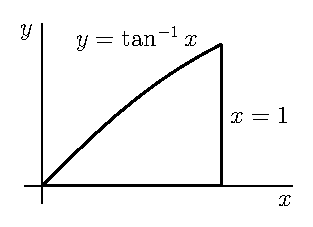
\includegraphics{graphE4bl}
\end{center}
\noindent (b) Volume: $ \dfrac{\pi^2}{2}-\pi$
\end{answer}

\begin{solution} (a) The sketch is the figure on  the left below.
By integration by parts with $u=\arctan x$, $\dee{v}=\dee{x}$,  $v=x$ and $\dee{u}=\frac{1}{1+x^2}\,\dee{x}$, and then the substitution $s=1+x^2$,
\begin{align*}
A&=\int_0^1\arctan x\ \dee{x}=\underbrace{ x\arctan x}_{uv}\Big|_0^1-\int_0^1\underbrace{\frac{x}{1+x^2}\,\dee{x}}_{v\dee{u}}
=\arctan 1-\half\log(1+x^2)\Big|_0^1\\
&=\frac{\pi}{4}-\frac{\log 2}{2}
\end{align*}

\begin{center}
       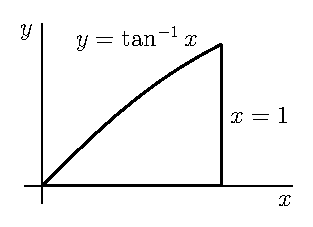
\includegraphics{graphE4bl}\qquad
       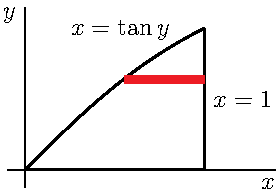
\includegraphics{graphE4br}
\end{center}

\noindent (b)
We'll use horizontal washers as in Example  \eref{CLP101}{eg rot yaxis}
of the %\href{http://www.math.ubc.ca/%7Efeldman/m101/clp/clp_notes_101.pdf}{CLP 101 notes}.
CLP--II text.
 \begin{itemize}
\item We cut $R$ into thin horizontal  strips of width $\dee{y}$ as in
the figure on the right above.

\item When we rotate $R$ about the $y$--axis, each strip sweeps out a thin
washer
\begin{itemize}
\item whose inner radius is $r_{in}=\tan y$ and outer radius is $r_{out}=1$, and
\item whose thickness is $\dee{y}$ and hence
\item whose volume $\pi(r_{out}^2 - r_{in}^2)\dee{y} = \pi(1-\tan^2 y)\dee{y}$.
\end{itemize}
\item As our bottommost strip is at $y=0$ and our topmost
strip is at $y=\frac{\pi}{4}$ (since at the top $x=1$ and $x=\tan y$), the total
\begin{align*}
\text{Volume}
&= \int _0^{\nicefrac{\pi}{4}} \pi(1-\tan^2 y)\ \dee{y}
= \int _0^{\nicefrac{\pi}{4}} \pi(2-\sec^2 y)\ \dee{y}
=\pi\big[2y -\tan y\big]_0^{\nicefrac{\pi}{4}} \\
&= \frac{\pi^2}{2}-\pi
\end{align*}
\end{itemize}
\end{solution}

%%%%%%%%%%%%%%%%%%%
%%%%%%%%%%%%%%%%%%%

\begin{question}[2016Q3] %% 6
Let $R$ be the region between the curves $T(x) = \sqrt{x}e^{3x}$ and $B(x) = \sqrt{x}(1+2x)$ on the interval $0 \le x \le 3$. (It is true that $T(x)\ge B(x)$ for all $0\le x\le 3$.) Compute the volume of the solid formed by rotating $R$ about the $x$-axis.
\end{question}

\begin{hint}
Your integral can be broken into two integrals, which yield to two different integration methods.
\end{hint}

\begin{answer}
$ \pi \left( \dfrac{17 e^{18}-4373}{36} \right)$
\end{answer}

\begin{solution}
For a fixed value of $x$, if we rotate about the $x$-axis, we form a washer of
inner radius $B(x)$ and outer radius $T(x)$ and hence of area $\pi [T(x)^2 - B(x)^2]$.
We integrate this function from $x=0$ to $x=3$ to find the total volume~$V$:
\begin{align*}
V &= \int_0^3 \pi [T(x)^2 - B(x)^2]\,\dee{x} \\
&= \pi \int_0^3 (\sqrt{x}e^{3x})^2 - (\sqrt{x}(1+2x))^2 \,\dee{x} \\
&= \pi \int_0^3  \big( xe^{6x} - (x+4x^2+4x^3) \big) \,\dee{x} \\
&=  \pi \int_0^3 xe^{6x} \,\dee{x}
       - \pi  \Big[ \frac{x^2}{2} + \frac{4x^3}{3} + x^4\Big]_{0}^3 \\
&= \pi \int_0^3 xe^{6x} \,\dee{x} - \pi \Big[\frac{3^2}{2} + \frac{4\cdot3^3}{3} + 3^4\Big]
\end{align*}
For the first integral, we use integration by parts with $u(x) = x$, $\dee{v} = e^{6x}\dee{x}$,
so that $\dee{u}=\dee{x}$ and $v(x)=\frac16e^{6x}$:
\begin{align*}
\int_0^3 xe^{6x} \,\dee{x}
&=\underbrace{ \frac{xe^{6x}}{6}}_{uv}\bigg|_{0}^3 - \int_0^3 \underbrace{\frac{1}{6}e^{6x} \,\dee{x} }_{v\dee{u}}\\
&= \frac{3e^{18}}{6} - 0 - \frac{1}{36} e^{6x} \bigg|_{0}^3
= \frac{e^{18}}{2} - \bigg( \frac{e^{18}}{36} - \frac1{36} \bigg).
\end{align*}
Therefore, the total volume is
\begin{align*}
  V = \pi \bigg[\frac{e^{18}}{2} - \bigg( \frac{e^{18}}{36} - \frac1{36} \bigg) \bigg]
               - \pi \bigg[\frac{3^2}{2} + \frac{4\cdot3^3}{3} + 3^4 \bigg]
    = \pi \bigg( \frac{17 e^{18}-4373}{36} \bigg).
\end{align*}
\end{solution}
%%%%%%%%%%%%%%%%%%%

\begin{Mquestion}[M105 2013A]
Let $f(0) = 1$, $f(2) = 3$ and $f'(2) = 4$.
Calculate
${\displaystyle\int_0^4 f''\big(\sqrt{x}\big)\,\dee{x}}$.
\end{Mquestion}

\begin{hint}
Think, first, about how to get rid of the square root in the argument of $f''$,
and, second, how to convert $f''$ into $f'$. Note that you are told that $f'(2) = 4$
and $f(0) = 1$, $f(2) = 3$.
\end{hint}

\begin{answer}
$12$
\end{answer}

\begin{solution}
To get rid of the square root in the argument of $f''$, we make the change of variables (also called ``substitution")
$x=t^2,\ \dee{x}=2t\,\dee{t}$.
\begin{align*}
\int_0^4 f''\big(\sqrt{x}\big)\,\dee{x}
&= 2\int_0^2 tf''(t)\,\dee{t}
\end{align*}
Then, to convert $f''$ into $f'$, we  integrate by parts with
$u=t$,  $\dee{v}=f''(t)\,\dee{t}$,    $v=f'(t) $.
\begin{align*}
\int_0^4 f''\big(\sqrt{x}\big)\,\dee{x}
&= 2\bigg\{\Big[\underbrace{tf'(t)}_{uv}\Big]_0^2-\int_0^2\!\!\!\underbrace{ f'(t)\,\dee{t}}_{v\dee{u}}\bigg\} \\
&=2\Big[tf'(t)-f(t)\Big]_0^2 \\
&=2\big[2f'(2)-f(2)+f(0)\big]=2\big[2\times 4-3+1\big]\\
&=12
\end{align*}


\end{solution}

%%%%%%%%%%%%%%%%%%%
\begin{question}
Evaluate $\displaystyle\lim_{n \to \infty}\sum_{i=1}^n \frac{2}{n}\left(\frac{2}{n}i-1\right)e^{\frac{2}{n}i-1}$\ .
\end{question}
\begin{hint}
Interpret the limit as a right Riemann sum.
\end{hint}
\begin{answer}
$\dfrac{2}{e}$
\end{answer}
\begin{solution}
As we saw in Section~\eref{CLP101}{sec:intdef} of the CLP--II text, there are many different ways to interpret a limit as a Riemann sum. In the absence of instructions that restrain our choices, we go with the most convenient interpretations.

With that in mind, we choose:
\begin{itemize}
\item that our Riemann sum is a right Riemann sum (because we see $i$, not $i-1$ or $i-\frac{1}{2}$)
\item $\Delta x = \frac{2}{n}$ (because it is multiplied by the rest of the integrand, and also shows up multiplied by $i$),
\item then $x_i = a+i\Delta x = \frac{2}{n}i-1$, which leads us to $a=-1$ and
\item $f(x) = xe^x$.
\item Finally, since $\Delta x = \frac{b-a}{n}=\frac{2}{n}$ and $a=-1$, we have $b=1$.
\end{itemize}

So, the limit is equal to the definite integral
\begin{align*}
\lim_{n \to \infty}\sum_{i=1}^n \frac{2}{n}\left(\frac{2}{n}i-1\right)e^{\frac{2}{n}i-1}&=\int_{-1}^1x e^x~\dee{x}
\intertext{which we evaluate using integration by parts with $u=x$, $\dee{v}=e^x\dee{x}$, $\dee{u}=\dee{x}$, and $v=e^x$.}
&=\Big[\underbrace{xe^x}_{uv} \Big]_{-1}^1 - \int_{-1}^1 \underbrace{e^x\dee{x}}_{v\dee{u}}\\
&=\left(e+\frac{1}{e}\right) - \left(e-\frac{1}{e}\right) = \frac{2}{e}
\end{align*}
\end{solution}

\section{Trigonometric Integrals}
%
% Copyright 2018 Joel Feldman, Andrew Rechnitzer and Elyse Yeager.
% This work is licensed under a Creative Commons Attribution-NonCommercial-ShareAlike 4.0 International License.
% https://creativecommons.org/licenses/by-nc-sa/4.0/
%
\questionheader{ex:s1.8}


\noindent
Recall that we are using $\log x$ to denote the logarithm of $x$ with
base $e$. In other courses it is often denoted $\ln x$.

%%%%%%%%%%%%%%%%%%
\subsection*{\Conceptual}
%%%%%%%%%%%%%%%%%%
\begin{Mquestion}
Suppose you want to evaluate $\displaystyle\int_0^{\pi/4} \sin x \cos^n x ~\dee{x}$ using the substitution $u=\cos x$. Which of the following need to be true for your substitution to work?
\begin{enumerate}[(a)]
\item $n$ must be even
\item $n$ must be odd
\item $n$ must be an integer
\item $n$ must be positive
\item $n$ can be any real number
\end{enumerate}
\end{Mquestion}
\begin{hint}
Go ahead and try it!
\end{hint}
\begin{answer}
(e)
\end{answer}
\begin{solution}
If $u=\cos x$, then $-\dee{u}=\dee{x}$. If $n \neq -1$, then
\begin{align*}
\int_0^{\pi/4} \sin x \cos^n x ~\dee{x}&= - \int_1^{1/\sqrt2} u^n \dee{u} = \left[-\frac{1}{n+1}u^{n+1}\right]_1^{1/\sqrt2}=\frac{1}{n+1}\left(1-\frac{1}{\sqrt{2}^{n+1}}\right)
\intertext{If $n=-1$, then}
\int_0^{\pi/4} \sin x \cos^n x ~\dee{x}&= - \int_1^{1/\sqrt2} u^n \dee{u} =
 - \int_1^{1/\sqrt2} \frac{1}{u} \dee{u} =\bigg[ -\log|u|\bigg]_1^{1/\sqrt2} \\
& =-\log\left(\frac{1}{\sqrt2}\right) = \frac{1}{2}\log 2
\end{align*}
So, (e) $n$ can be any real number.
\end{solution}
%%%%%%%%%%%%%%%%%%%

\begin{question}
Evaluate $\displaystyle\int \sec^n x \tan x \dee{x}$, where $n$ is a strictly positive integer.\end{question}
\begin{hint}
Use the substitution $u=\sec x$.
\end{hint}
\begin{answer}
$ \dfrac{1}{n}\sec^n x +C$
\end{answer}
\begin{solution}
We use the substitution $u=\sec x$,  $\dee{u}=\sec x \tan x ~\dee{x}$.
\begin{align*}
\int \sec^n x \tan x \dee{x}&=\int \sec^{n-1}x \cdot \sec x \tan x~\dee{x} = \int u^{n-1}\dee{u}
\intertext{Since $n$ is positive, $n-1 \neq -1$, so we antidifferentiate using the power rule.}
&=\frac{u^n}{n}+C = \frac{1}{n}\sec^n x +C
\end{align*}
\end{solution}
%%%%%%%%%%%%%%%%%%%


\begin{question}
Derive the identity $\tan^2 x +1 = \sec^2 x$ from the easier-to-remember identity $\sin^2x+\cos^2 x =1$.
\end{question}
\begin{hint}
Divide both sides of the second identity by $\cos^2 x$.
\end{hint}
\begin{answer}
We divide both sides by $\cos^2 x$, and simplify.
\begin{align*}
\sin^2x+\cos^2 x &=1
\\\frac{\sin^2x+\cos^2 x }{\cos^2 x}&=\frac{1}{\cos^2 x}
\\\frac{\sin^2x}{\cos^2 x}+1&=\sec^2 x
\\\tan^2 x+1&=\sec^2 x
\end{align*}

\end{answer}
\begin{solution}
We divide both sides by $\cos^2 x$, and simplify.
\begin{align*}
\sin^2x+\cos^2 x &=1
\\\frac{\sin^2x+\cos^2 x }{\cos^2 x}&=\frac{1}{\cos^2 x}
\\\frac{\sin^2x}{\cos^2 x}+1&=\sec^2 x
\\\tan^2 x+1&=\sec^2 x
\end{align*}
\end{solution}
%%%%%%%%%%%%%%%%%%%



%%%%%%%%%%%%%%%%%%
\subsection*{\Procedural}
%%%%%%%%%%%%%%%%%%

\Instructions{Questions \ref{1.8sincos1} through \ref{1.8sincos2} deal with powers of sines and cosines. Review Section~\eref{CLP101}{sec:sincos} in the CLP-2 text for integration strategies.}

\begin{question}[M105 2015A]\label{1.8sincos1}
Evaluate $\displaystyle\int\cos^3x\,\dee{x}$.
\end{question}

\begin{hint}
See Example \eref{CLP101}{eg:TRGINTa} in the
%\href{http://www.math.ubc.ca/%7Efeldman/m101/clp/clp_notes_101.pdf}{CLP-2 text}.
CLP-2 text. Note that the power of cosine is odd, and the power of sine is even (it's zero).
\end{hint}

\begin{answer}
$ \sin x-\dfrac{\sin^3 x}{3} +C$
\end{answer}

\begin{solution}
The power of cosine is odd, and the power of sine is even (zero).  Following the strategy in the text, we make the substitution $u=\sin x$, so that $\dee{u}=\cos x\,\dee{x}$
and $\cos^2 x = 1-\sin^2 x = 1-u^2$:
\begin{align*}
\int \cos^3x\,\dee{x}
&=\int (1-\sin^2x)\cos x\,\dee{x}
=\int (1-u^2)\,\dee{u}\\
&=u-\frac{u^3}3+C
=\sin x-\frac{\sin^3 x}{3}+C
\end{align*}
\end{solution}
%%%%%%%%%%%%%%%%%%%


\begin{Mquestion}[2014D]
Evaluate $\displaystyle\int_0^\pi\cos^2x\,\dee{x}$.
\end{Mquestion}

\begin{hint}
See Example \eref{CLP101}{eg:TRGINTb} in the
%\href{http://www.math.ubc.ca/%7Efeldman/m101/clp/clp_notes_101.pdf}{CLP-2 text}.
CLP-2 text. All you need is a helpful trig identity.
\end{hint}

\begin{answer}
$\dfrac{\pi}{2}$
\end{answer}

\begin{solution}
Using the trig identity $\cos^2 x=\dfrac{1+\cos(2x)}{2}$, we have
\begin{alignat*}{3}
\int \cos^2 x\dee{x}
&= \frac{1}{2}\int_0^\pi \big[1+\cos(2x)\big]\dee{x}  %\\[0,1in]
&= \frac{1}{2} \Big[x+\frac{1}{2}\sin(2x)\Big]_0^\pi
&=\frac{\pi}{2}
\end{alignat*}
\end{solution}
%%%%%%%%%%%%%%%%%%%



\begin{question}[2016Q3]
Evaluate $\displaystyle\int\sin^{36}t\,\cos^3t\,\dee{t}$.
\end{question}

\begin{hint}
The power of cosine is odd, so we can reserve one cosine for $\dee{u}$, and turn the rest into sines using the identity $\sin^2 x + \cos^2 x =1$.
\end{hint}

\begin{answer}
$\dfrac{\sin^{37}t}{37}-\dfrac{\sin^{39}t}{39}+C$
\end{answer}

\begin{solution}
Since the power of cosine is odd, following the strategies in the text, we make the substitution $u=\sin t$, so that $\dee{u}=\cos t\,\dee{t}$
and $\cos^2 t = 1-\sin^2 t = 1-u^2$.
\begin{align*}
\int\sin^{36}t\cos^3t\,\dee{t}
&=\int\sin^{36}t \, (1-\sin^2t)\cos t\,\dee{t}
=\int u^{36}(1-u^2)\,\dee{u}\\
&=\frac{u^{37}}{37}-\frac{u^{39}}{39}+C
=\frac{\sin^{37}t}{37}-\frac{\sin^{39}t}{39}+C
\end{align*}
\end{solution}
%%%%%%%%%%%%%%%%%%%


\begin{Mquestion}
Evaluate $\displaystyle\int \dfrac{\sin^3 x}{\cos^4 x} ~\dee{x}$.
\end{Mquestion}
\begin{hint}
Since the power of sine is odd (and positive), we can reserve one sine for $\dee{u}$, and turn the rest into cosines using the identity $\sin^2  + \cos^2 x =1$.
\end{hint}
\begin{answer}
$\dfrac{1}{3\cos^3 x} - \dfrac{1}{\cos x}+C$
\end{answer}
\begin{solution}
Since the power of sine is odd (and positive), we can reserve one sine for $\dee{u}$, and turn the rest into cosines using the identity $\sin^2  + \cos^2 x =1$. This allows us to use the substitution $u=\cos x$, $\dee{u}=-\sin x~\dee{x}$, and $\sin^2 x = 1-\cos^2 x = 1-u^2$.
\begin{align*}
\int \dfrac{\sin^3 x}{\cos ^4 x} ~\dee{x}&=\int \frac{\sin^2 x}{\cos^4 x}\sin x~\dee{x}
=\int -\frac{1-u^2}{u^4}\dee{u}\\
&=\int\left( -\frac{1}{u^{4}}+\frac{1}{u^{2}}\right)~\dee{u} = \frac{1}{3u^3}-\frac{1}{u}+C\\
&=\frac{1}{3\cos^3 x} - \frac{1}{\cos x}+C
\end{align*}
\end{solution}

%%%%%%%%%%%%%%%%%%%
\begin{question}
Evaluate $\displaystyle\int_0^{\pi/3} \sin^{4}x~\dee{x}$.
\end{question}
\begin{hint}
When we have even powers of sine and cosine both, we use the identities in the last two lines of Equation~\eref{CLP101}{eq:TRGINTtrigidentityC} in the CLP-2 text.
\end{hint}
\begin{answer}
$\displaystyle\frac{\pi}{8} -\frac{9\sqrt3}{64}$
\end{answer}
\begin{solution}
Both sine and cosine have even powers (four and zero, respectively), so we don't have the option of using a substitution like $u=\sin x$ or $u=\cos x$. Instead, we use the identity $\sin^2 \theta = \dfrac{1-\cos(2\theta)}{2}$.
\begin{align*}
\int_0^{\pi/3} \sin^{4}x~\dee{x} &= \int_0^{\pi/3} \left(\sin^{2}x\right)^2~\dee{x}
= \int_0^{\pi/3} \left(\frac{1-\cos(2x)}{2}\right)^2~\dee{x}\\
&=\frac{1}{4}\int_0^{\pi/3}\left(1-2\cos(2x)+\cos^2(2x)\right)~\dee{x}
\\&=\frac{1}{4}\int_0^{\pi/3}\left(1-2\cos(2x)\right)~\dee{x}+\frac{1}{4}\int_0^{\pi/3}\cos^2(2x)~\dee{x}
\intertext{We can antidifferentiate the first integral right away. For the second integral, we use the identity \quad $\cos^2 \theta = \dfrac{1+\cos(2\theta)}{2}$,\quad with $\theta=2x$.}
&=\frac{1}{4}\Big[x - \sin(2x)\Big]_{0}^{\pi/3} + \frac{1}{8}\int_0^{\pi/3}(1+\cos(4x))~\dee{x}\\
&=\frac{1}{4}\left[\frac{\pi}{3}-\frac{\sqrt{3}}{2}\right]+\frac{1}{8}\Big[x+\frac{1}{4}\sin(4x)\Big]_0^{\pi/3}\\
&=\frac{1}{4}\left[\frac{\pi}{3}-\frac{\sqrt{3}}{2}\right]+\frac{1}{8}\left[\frac{\pi}{3}-\frac{\sqrt{3}}{8}\right]\\
&=\frac{\pi}{8} -\frac{9\sqrt3}{64}
\end{align*}
\end{solution}

%%%%%%%%%%%%%%%%%%%

%%%%%%%%%%%%%%%%%%%
\begin{question}
Evaluate $\displaystyle\int \sin^{5}x~\dee{x}$.
\end{question}
\begin{hint}
Since the power of sine is odd, you can use the substitution $u=\cos x$.
\end{hint}
\begin{answer}
$-\cos x + \dfrac{2}{3}\cos^3 x - \dfrac{1}{5}\cos^5 x +C$
\end{answer}
\begin{solution}
Since the power of sine is odd, we can reserve one sine for $\dee{u}$, and change the remaining four into cosines. This sets us up to use the substitution $u=\cos x$, $\dee{u}=-\sin x~\dee{x}$.
\begin{align*}
\int \sin^{5}x~\dee{x}&=\int \sin^4 x \cdot \sin x~\dee{x} = \int (1-\cos^2 x)^2 \sin x~\dee{x}
\\&=-\int (1-u^2)^2~\dee{u}
= -\int (1-2u^2+u^4)\dee{u}\\
&=-u+\frac{2}{3}u^3-\frac{1}{5}u^5+C\\
&=-\cos x + \frac{2}{3}\cos^3 x - \frac{1}{5}\cos^5 x +C
\end{align*}
\end{solution}

%%%%%%%%%%%%%%%%%%%


\begin{Mquestion}\label{1.8sincos2}
Evaluate $\displaystyle\int \sin^{1.2}x\cos x ~\dee{x}$.
\end{Mquestion}
\begin{hint}
Which substitution will work better: $u=\sin x$, or $u=\cos x$?
\end{hint}
\begin{answer}
$\dfrac{1}{2.2}\sin^{2.2}x+C$
\end{answer}
\begin{solution}
If we use the substitution $u=\sin x$, then $\dee{u}=\cos x~\dee{x}$, which very conveniently shows up in the integrand.
\begin{align*}
\int \sin^{1.2}x\cos x ~\dee{x}&=\int u^{1.2}\dee{u} = \frac{u^{2.2}}{2.2}+C = \frac{1}{2.2}\sin^{2.2}x+C
\end{align*}
Note this is exactly the strategy described in the text when the power of cosine is odd. The non-integer power of sine doesn't cause a problem.
\end{solution}


%%%%%%%%%%%%%%%%%%%
%%%%%%%%%%%%%%%%%%%
%%%%%%%%%%%%%%%%%%%
\Instructions{Questions \ref{1.8tansec1} through \ref{1.8tansec2} deal with powers of tangents and secants. Review Section~\eref{CLP101}{sec:tansec} in the CLP-2 text for strategies.}
%%%%%%%%%%%%%%%%%%%
%%%%%%%%%%%%%%%%%%%
%%%%%%%%%%%%%%%%%%%
\begin{Mquestion}
Evaluate $\displaystyle\int \tan x \sec^2 x \dee{x}$.
\end{Mquestion}
\begin{hint}
Try a substitution.
\end{hint}
\begin{answer}
$\dfrac{1}{2}\tan^2 x+C$, or equivalently, $\dfrac{1}{2}\sec^2  +C$
\end{answer}
\begin{solution}
\begin{description}
\item[Solution 1:] Let's use the substitution $u=\tan x$, $\dee{u} = \sec^2 x~\dee{x}$:
\[\int \tan x \sec^2 x \dee{x} = \int u~\dee{u} = \frac{1}{2}u^2+C = \frac{1}{2}\tan^2 x +C\]
\item[Solution 2:]
We can also use the substitution $u=\sec x$, $\dee{u} = \sec x \tan x~\dee{x}$:
\[ \int\tan x \sec^2 x \dee{x} = \int u~\dee{u} = \frac{1}{2}u^2+C = \frac{1}{2}\sec^2 x +C\]
\end{description}
We note that because $\tan^2x$ and $\sec^2 x$ only differ by a constant, the two answers are equivalent.
\end{solution}
%%%%%%%%%%%%%%%%%%%
\begin{Mquestion}[2015A]\label{1.8tansec1}
Evaluate $\displaystyle\int \tan^3 x \sec^5x \,\dee{x}$.
\end{Mquestion}

\begin{hint}
For practice, try doing this in two ways, with different
substitutions.
\end{hint}

\begin{answer}
$\dfrac{1}{7}\sec^7 x -\dfrac{1}{5}\sec^5 x + C$
\end{answer}

\begin{solution}
\begin{description}
\item[Solution 1:]
Substituting $u=\cos x$, $\dee{u}=-\sin x\,\dee{x}$, $\sin^2 x= 1-\cos^2x=1-u^2$,
gives
\begin{align*}
\int \tan^3 x \sec^5x \,\dee{x}
&=\int\frac{\sin^3 x}{\cos^8 x}\,\dee{x}
=\int\frac{(1-\cos^2 x)\sin x}{\cos^8 x}\,\dee{x}
=-\int\frac{1-u^2}{u^8}\,\dee{u} \\
&=-\Big[\frac{u^{-7}}{-7}-\frac{u^{-5}}{-5}\Big]+C
=\frac{1}{7}\sec^7 x -\frac{1}{5}\sec^5 x + C
\end{align*}

\item[Solution 2:]
 Alternatively, substituting $u=\sec x$, $\dee{u}=\sec x\tan x\,\dee{x}$,
$\tan^2 x= \sec^2x-1=u^2-1$,
gives
\begin{align*}
\int \tan^3 x \sec^5x \,\dee{x}
&=\int \tan^2 x \sec^4x\ (\tan x\sec x)\,\dee{x}
=\int (u^2-1) u^4\,\dee{u} \\
&=\Big[\frac{u^{7}}{7}-\frac{u^{5}}{5}\Big]+C
=\frac{1}{7}\sec^7 x -\frac{1}{5}\sec^5 x + C
\end{align*}
\end{description}
\end{solution}
%%%%%%%%%%%%%%%%%%%

\begin{Mquestion}[2016Q3]
Evaluate $\displaystyle\int\sec^4x\,\tan^{46}x\,\dee{x}$.
\end{Mquestion}

\begin{hint}
 A substitution will work.
See Example \eref{CLP101}{eg:TRGINTe} in the
%\href{http://www.math.ubc.ca/%7Efeldman/m101/clp/clp_notes_101.pdf}{CLP-2 text}.
CLP-2 text for a template for integrands with even powers of secant.
\end{hint}

\begin{answer}
$\displaystyle\frac{\tan^{49}x}{49}+\frac{\tan^{47}x}{47}+C$
\end{answer}

\begin{solution}
Use the substitution $u=\tan x$, so that $\dee{u}=\sec^2 x\,\dee{x}$:
\begin{align*}
\int\sec^4x\,\tan^{46}x\,\dee{x}
&=\int(\tan^2x+1) \tan^{46}x\, \sec^2 x\,\dee{x} =\int (u^2+1)u^{46}\,\dee{u} \\
&=\frac{u^{49}}{49}+\frac{u^{47}}{47}+C
=\frac{\tan^{49}x}{49}+\frac{\tan^{47}x}{47}+C
\end{align*}
\end{solution}
%%%%%%%%%%%%%%%%%%%



\begin{question}\label{1.8_oddtanonesec}
Evaluate $\displaystyle\int \tan^3 x \sec^{1.5} x ~\dee{x}$.
\end{question}
\begin{hint}
Try the substitution $u=\sec x$.
\end{hint}
\begin{answer}
$\dfrac{1}{3.5}\sec^{3.5}x - \dfrac{1}{1.5}\sec^{1.5}x+C$
\end{answer}
\begin{solution}
We use the substitution $u=\sec x$, $\dee{u} = \sec x \tan x~\dee{x}$. Then $\tan^2 x = \sec^2 x - 1 = u^2-1$.
\begin{align*}
\int \tan^3 x \sec^{1.5} x ~\dee{x} &= \int \tan^2 x \cdot \sec^{0.5}x \cdot \sec x \tan x \dee{x}\\
&=\int(u^2-1)u^{0.5}~\dee{u} = \int \left(u^{2.5} - u^{0.5}\right)~\dee{u}\\
&=\frac{u^{3.5}}{3.5} - \frac{u^{1.5}}{1.5}+C\\
&=\frac{1}{3.5}\sec^{3.5}x - \frac{1}{1.5}\sec^{1.5}x+C
\end{align*}
Note this solution used the same method as Example~\eref{CLP101}{eg:TRGINTf}  in the CLP-2 text for the case that the power of tangent is odd and there is at least one secant.
\end{solution}
%%%%%%%%%%%%%%%%%%%





\begin{question}\label{1.8_oddtanonesec2}
Evaluate $\displaystyle\int \tan^3x\sec^2x~\dee{x}$.
\end{question}
\begin{hint}
Compare to Question~\ref{1.8_oddtanonesec}.
\end{hint}
\begin{answer}
$\dfrac{1}{4}\sec^4 x - \dfrac{1}{2}\sec^2 x +C$
\end{answer}
\begin{solution}
As in Question~\ref{1.8_oddtanonesec}, we have an odd power of tangent and at least one secant. So, we can use the substitution $u=\sec x$, $\dee{u}=\sec x \tan x~\dee{x}$, and $\tan^2 x = \sec^2 x -1=u^2-1$.
\begin{align*}
\int \tan^3x\sec^2x~\dee{x}&=\int \tan^2 x \sec x \cdot \sec x \tan x~\dee{x}\\
&=\int(u^2-1)u~\dee{u} = \int \left(u^3-u\right)~\dee{u}\\
&=\frac{1}{4}u^4 - \frac{1}{2}u^2+C\\
&=\frac{1}{4}\sec^4 x - \frac{1}{2}\sec^2 x +C
\end{align*}
\end{solution}
%%%%%%%%%%%%%%%%%%%

\begin{question}
Evaluate $\displaystyle\int \tan^4 x \sec^2 x ~\dee{x}$.
\end{question}
\begin{hint}
What is the derivative of tangent?
\end{hint}
\begin{answer}
$\dfrac{1}{5}\tan^5 x +C$
\end{answer}
\begin{solution}
In contrast to Questions~\ref{1.8_oddtanonesec} and \ref{1.8_oddtanonesec2}, we do not have an odd power of tangent, so we should consider a different substitution. Luckily, if we choose $u=\tan x$, then $\dee{u}=\sec^2 x~\dee{x}$, and this fits our integrand nicely.
\begin{align*}
\int \tan^4 x \sec^2 x ~\dee{x}&=\int u^4~\dee{u}=\frac{1}{5}u^5+C = \frac{1}{5}\tan^5 x +C
\end{align*}
\end{solution}
%%%%%%%%%%%%%%%%%%%



\begin{question}
Evaluate $\displaystyle\int \tan^3 x \sec^{-0.7}x ~\dee{x}$.
\end{question}
\begin{hint}
Don't be scared off by the non-integer power of secant. You can still use the strategies in the notes for an odd power of tangent.
\end{hint}
\begin{answer}
$\dfrac{1}{1.3}\sec^{1.3}x + \dfrac{1}{0.7}\cos^{0.7}x+C$
\end{answer}
\begin{solution}
\begin{description}
\item[Solution 1:] Since the power of tangent is odd, let's try to use the substitution $u=\sec x$, $\dee{u} = \sec x \tan x ~\dee{x}$, and $\tan^2 x = \sec^2 x -1 = u^2-1$, as in Questions~\ref{1.8_oddtanonesec} and \ref{1.8_oddtanonesec2}. In order to make this work, we need to see $\sec x \tan x~\dee{x}$ in the integrand, so we do a little algebraic manipulation.
\begin{align*}
\int \tan^3 x \sec^{-0.7}x ~\dee{x}&= \int \dfrac{\tan^3 x}{\sec^{0.7 x}}~\dee{x}
= \int \dfrac{\tan^3 x}{\sec^{1.7 x}}\sec x~\dee{x}\\
&=\int \frac{\tan^2x}{\sec^{1.7}x}\cdot \sec x \tan x~\dee{x}\\
&=\int \frac{u^2-1}{u^{1.7}}~\dee{u} = \int \left(u^{0.3}-u^{-1.7}\right)~\dee{u}\\
&=\frac{u^{1.3}}{1.3} + \frac{1}{0.7u^{0.7}}+C\\
&=\frac{1}{1.3}\sec^{1.3}x + \frac{1}{0.7\sec^{0.7}x}+C\\
&=\frac{1}{1.3}\sec^{1.3}x + \frac{1}{0.7}\cos^{0.7}x+C
\end{align*}
\item[Solution 2:] Let's convert the secants and tangents to sines and cosines.
\begin{align*}
\int \tan^3 x \sec^{-0.7}x ~\dee{x}&=
\int \frac{\sin^3 x}{\cos^3 x}\cdot \cos^{0.7}x~\dee{x}\\
&=\int\frac{\sin^3 x}{\cos^{2.3}x}~\dee{x}=\int \frac{\sin^2 x}{\cos^{2.3}x}\cdot\sin x~\dee{x}
\intertext{Using the substitution $u=\cos x$, $\dee{u}=-\sin~\dee{x}$, and $\sin^2 x = 1-\cos^2 x = 1-u^2$:}
& = -\int\frac{1-u^2}{u^{2.3}}~\dee{u} = \int \left(-u^{-2.3}+u^{-0.3}\right)~\dee{u}\\
&=\frac{1}{1.3}u^{-1.3} + \frac{1}{0.7}u^{0.7}+C\\
&=\dfrac{1}{1.3}\sec^{1.3}x + \dfrac{1}{0.7}\cos^{0.7}x+C
\end{align*}
\end{description}
\end{solution}
%%%%%%%%%%%%%%%%%%%




\begin{question}
Evaluate $\displaystyle\int \tan^5 x  ~\dee{x}$.
\end{question}
\begin{hint}
 Since there are no secants in the problem, it's difficult to use the substitution $u=\sec x$ that we've enjoyed in the past.
 Example~\eref{CLP101}{eg:TRGINTh} in the CLP-2 text provides a template for antidifferentiating an odd power of tangent.
\end{hint}
\begin{answer}
$=\dfrac{1}{4}\sec^4 x - \sec^2 x + \log|\sec x|+C$
\end{answer}
\begin{solution}
We replace $\tan x$ with $\dfrac{\sin x}{\cos x}$.
\begin{align*}
\int \tan^5 x~\dee{x}&=\int\left(\frac{\sin x}{\cos x}\right)^5~\dee{x} = \int\frac{\sin^4 x}{\cos^5 x}\cdot \sin x~\dee{x}
\intertext{Now we use the substitution $u=\cos x$, $\dee{u}=-\sin x~\dee{x}$, and $\sin^2 x = 1-\cos^2 x = 1-u^2$.}
&=-\int\frac{(1-u^2)^2}{u^5}~\dee{u} = \int \left(-u^{-5}+2u^{-3}-u^{-1}\right)~\dee{u}\\
&=\frac{1}{4}u^{-4} - u^{-2}-\log|u|+C\\
&=\dfrac{1}{4}\sec^4 x - \sec^2 x - \log|\cos x|+C\\
&=\dfrac{1}{4}\sec^4 x - \sec^2 x + \log|\sec x|+C
\end{align*}
where in the last line, we used the logarithm rule $\log(b^a) = a\log b$, with $
b^a = \cos x = \left(\sec x\right)^{-1}$.
\end{solution}
%%%%%%%%%%%%%%%%%%%
\begin{Mquestion}\label{1.8_tan6} Evaluate $\displaystyle\int_0^{\pi/6} \tan^6 x ~\dee{x}$.
\end{Mquestion}
\begin{hint}
Integrating even powers of tangent is surprisingly different from integrating odd powers of tangent. You'll want to use the identity $\tan^2x  = \sec^2 x -1$, then use the substitution $u=\tan x$, $\dee{u}=\sec^2 x~\dee{x}$ on (parhaps only a part of) the resulting integral.
 Example~\eref{CLP101}{eg:TRGINTi} in the CLP-2 text show you how this can be accomplished.
\end{hint}
\begin{answer}
$\dfrac{41}{45\sqrt{3}} - \dfrac{\pi}{6}$
\end{answer}
\begin{solution}
Integrating even powers of tangent is surprisingly different from integrating odd powers of tangent. For even powers, we use the identity $\tan^2x  = \sec^2 x -1$, then use the substitution $u=\tan x$, $\dee{u}=\sec^2 x~\dee{x}$ on (parhaps only a part of) the resulting integral.
\begin{align*}
\int_0^{\pi/6} \tan^6 x ~\dee{x}&=\int_0^{\pi/6} \tan^4 x(\sec^2 x -1) ~\dee{x}\\
&=\int_0^{\pi/6} \bigg(\underbrace{\tan^4 x \sec^2 x}_{u^4~\dee{u}} - \tan^4 x\bigg)~\dee{x}\\
&=\int_0^{\pi/6} \bigg(\tan^4 x \sec^2 x - \tan^2 x(\sec^2 x-1)\bigg)~\dee{x}
\\&=\int_0^{\pi/6}\bigg( \tan^4 x \sec^2 x - \underbrace{\tan^2 x\sec^2 x}_{u^2~\dee{u}}+\tan^2 x\bigg)~\dee{x}
\\&=\int_0^{\pi/6}\bigg( \tan^4 x \sec^2 x - \tan^2 x\sec^2 x+(\underbrace{\sec^2x}_{\dee{u}}-1)\bigg)~\dee{x}
\\&=\int_0^{\pi/6}\left( \tan^4 x  - \tan^2 x+1\right)\sec^2 x~\dee{x} - \int_0^{\pi/6} 1\dee{x}
\intertext{ Note $\tan(0)=0$, and $\tan(\pi/6)=1/\sqrt{3}$.}
&=\int_0^{1/\sqrt{3}}(u^4-u^2+1)~\dee{u} - \big[ x\big]_0^{\pi/6}\\
&=\left[\frac{1}{5}u^5 - \frac{1}{3}u^3+u\right]_0^{1/\sqrt{3}} - \frac{\pi}{6}\\
&=\frac{1}{5\sqrt{3}^5} - \frac{1}{3\sqrt{3}^3}+\frac{1}{\sqrt{3}}-\frac{\pi}{6}\\
&=\dfrac{41}{45\sqrt{3}} - \dfrac{\pi}{6}
\end{align*}
\end{solution}
%%%%%%%%%%%%%%%%%%%



\begin{question}
Evaluate $\displaystyle\int_0^{\pi/4} \tan^8 x \sec^4 x ~\dee{x}$.
\end{question}
\begin{hint}
Since there is an even power of secant in the integrand, we can use the substitution $u=\tan x$.
\end{hint}
\begin{answer}
$\dfrac{1}{11}+\dfrac{1}{9}$
\end{answer}
\begin{solution}
Since there is an even power of secant in the integrand, we can reserve two secants for $\dee{u}$ and change the rest to tangents. That sets us up nicely to use the substitution $u=\tan x$, $\dee{u}=\sec^2 x~\dee{x}$. Note $\tan(0)=0$ and $\tan(\pi/4)=1$.
\begin{align*}
\int_0^{\pi/4} \tan^8 x \sec^4 x ~\dee{x}&=\int_0^{\pi/4} \tan^8 x~( \tan^2 x+1) \sec^2 x~\dee{x}\\&=\int_0^{1} u^8 ~( u^2 +1) ~\dee{u}\\
&=\int_0^1 u^{10}+u^8~\dee{u}\\
&=\frac{1}{11}+\frac{1}{9}
\end{align*}
\end{solution}
%%%%%%%%%%%%%%%%%%%



\begin{question}\label{1.8tansec2}
Evaluate $\displaystyle\int \tan x \sqrt{\sec x} ~\dee{x}$.
\end{question}
\begin{hint}
How have we handled integration in the past that involved an odd power of tangent?
\end{hint}
\begin{answer}
$2\sqrt{\sec x}+C$
\end{answer}
\begin{solution}
\begin{description}
\item[Solution 1:] Let's use the substitution $u=\sec x$, $\dee{u}=\sec x \tan x~\dee{x}$. In order to make this work, we need to see $\sec x \tan x$ in the integrand, so we start with some algebraic manipulation.
\begin{align*}
\int \tan x \sqrt{\sec x}\left(\frac{\sqrt{\sec x}}{\sqrt{\sec x}}\right) ~\dee{x}&=\int \frac{1}{\sqrt{\sec x}}\sec x\tan x~\dee{x}\\
&=\int \frac{1}{\sqrt{u}}~\dee{u}=2\sqrt{u}+C\\
&=2\sqrt{\sec x}+C
\end{align*}
\item[Solution 2:] Let's turn our secants and tangents into sines and cosines.
\begin{align*}
\int \tan x \sqrt{\sec x}~\dee{x}&=\int \frac{\sin x}{\cos x\cdot\sqrt{\cos x}}~\dee{x}=\int \frac{\sin x}{\cos^{1.5}x}~\dee{x}
\intertext{We use the substitution $u=\cos x$, $\dee{u}=-\sin x~\dee{x}$.}
&=\int -u^{-1.5}~\dee{u}=\frac{2}{\sqrt{u}}+C\\
&=2\sqrt{\sec x}+C
\end{align*}
\end{description}
\end{solution}
%%%%%%%%%%%%%%%%%%%

\begin{Mquestion}
Evaluate $\displaystyle\int \sec^{8}\theta \tan^{e}\theta ~\dee{\theta}$.
\end{Mquestion}
\begin{hint}
Remember $e$ is some constant. What are our strategies when the power of secant is even and positive? We've seen one such substitution in Example~\eref{CLP101}{eg:TRGINTfredux}
of the CLP-2 text.
\end{hint}
\begin{answer}
$\tan^{e+1}\theta\left(
\dfrac{\tan^{6}\theta}{7+e}+\dfrac{3\tan^4\theta}{5+e}+\dfrac{3\tan^2\theta}{3+e}+\dfrac{1}{1+e}
\right)+C$
\end{answer}
\begin{solution}
Since the power of secant is even and positive, we can reserve two secants for $\dee{u}$, and change the rest into tangents, setting the stage for the substitution $u = \tan \theta$, $\dee{u}=\sec^2 \theta~\dee{\theta}$.
\begin{align*}
\int \sec^{8}\theta \tan^{e}\theta ~\dee{\theta}&=\int \sec^6 \theta \tan^e \theta \sec^2 \theta~\dee{\theta}\\
&=\int (\tan^2 \theta +1)^3  \tan^e \theta \sec^2 \theta~\dee{\theta}\\
&=\int (u^2+1)^3 \cdot u^e ~\dee{u}\\
&=\int (u^6+3u^4 +3u^2+1) \cdot u^e ~\dee{u}\\
&=\int (u^{6+e}+3u^{4+e} +3u^{2+e}+ u^e) ~\dee{u}\\
&=\frac{1}{7+e}u^{7+e}+\frac{3}{5+e}u^{5+e}+\frac{3}{3+e}u^{3+e}+\frac{1}{1+e}u^{1+e}+C
\\
&=\frac{1}{7+e}\tan^{7+e}\theta+\frac{3}{5+e}\tan^{5+e}\theta+\frac{3}{3+e}\tan^{3+e}\theta+\frac{1}{1+e}\tan^{1+e}\theta+C\\
&=\tan^{1+e}\theta\left(
\frac{\tan^{6}\theta}{7+e}+\frac{3\tan^4\theta}{5+e}+\frac{3\tan^2\theta}{3+e}+\frac{1}{1+e}
\right)+C
\end{align*}
\end{solution}
%%%%%%%%%%%%%%%%%%%





%%%%%%%%%%%%%%%%%%
\subsection*{\Application}
%%%%%%%%%%%%%%%%%%



\begin{Mquestion}[2001D]
A reduction formula.
\begin{enumerate}[(a)]
\item
Let $n$ be a positive integer with $n\ge 2$.
Derive the reduction formula
\[\int\tan^n(x)\,\dee{x}=\frac{\tan^{n-1}(x)}{n-1}
-\int\tan^{n-2}(x)\,\dee{x}.\]
\item
Calculate $\displaystyle\int_0^{\pi/4}\tan^6(x)\,\dee{x}$.
\end{enumerate}
\end{Mquestion}

\begin{hint}
See Example \eref{CLP101}{eg:TRGINTi} in the
%\href{http://www.math.ubc.ca/%7Efeldman/m101/clp/clp_notes_101.pdf}{CLP-2 text}.
CLP-2 text for a strategy for integrating powers of tangent.
\end{hint}

\begin{answer} (a) Using the trig identity $\tan^2x=\sec^2 x-1$ and the substitution
$y=\tan x$, $\dee{y}=\sec^2 x\  \dee{x}$,
\begin{alignat*}{3}
\int\tan^nx\ \dee{x}
&=\int\tan^{n-2}x\ \tan^2x\ \dee{x}
&&=\int\tan^{n-2}x\ \sec^2x\ \dee{x}-\int\tan^{n-2}x\ \dee{x}\\
&=\int y^{n-2}\,\dee{y}-\int\tan^{n-2}x\ \dee{x}
&&=\frac{y^{n-1}}{n-1}-\int\tan^{n-2}x\ \dee{x}\\
&=\frac{\tan^{n-1}x}{n-1} -\int\tan^{n-2}x\ \dee{x}
\end{alignat*}

 (b) $\displaystyle\frac{13}{15}-\frac{\pi}{4}\approx0.0813$
\end{answer}

\begin{solution} (a)
Using the trig identity $\tan^2x=\sec^2 x-1$ and the substitution
$y=\tan x$, $\dee{y}=\sec^2 x\  \dee{x}$,
\begin{alignat*}{3}
\int\tan^nx\ \dee{x}
&=\int\tan^{n-2}x\ \tan^2x\ \dee{x}
&&=\int\tan^{n-2}x\ \sec^2x\ \dee{x}-\int\tan^{n-2}x\ \dee{x}\\
&=\int y^{n-2}\,\dee{y}-\int\tan^{n-2}x\ \dee{x}
&&=\frac{y^{n-1}}{n-1}-\int\tan^{n-2}x\ \dee{x}\\
&=\frac{\tan^{n-1}x}{n-1} -\int\tan^{n-2}x\ \dee{x}
\end{alignat*}

\noindent (b)
By the reduction formula of part (a),
\begin{align*}
\int_0^{\pi/4}\tan^n(x)\,\dee{x}&=
\left[\frac{\tan^{n-1}x}{n-1}\right]_{0}^{\pi/4}-\int_0^{\pi/4}\tan^{n-2}(x)\,\dee{x}\\
&=\frac{1}{n-1}-\int_0^{\pi/4}\tan^{n-2}(x)\,\dee{x}
\end{align*}
for all integers $n\ge 2$, since $\tan 0=0$ and $\tan\frac{\pi}{4}=1$.
We apply this reduction formula, with $n=6,4,2$.
\begin{align*}
\int_0^{\pi/4}\tan^6(x)\,\dee{x}
&=\frac{1}{5}-\int_0^{\pi/4}\tan^4(x)\,\dee{x}
=\frac{1}{5}-\frac{1}{3}+\int_0^{\pi/4}\tan^2(x)\,\dee{x}
=\frac{1}{5}-\frac{1}{3}+1-\int_0^{\pi/4}\,\dee{x}\cr
&=\frac{1}{5}-\frac{1}{3}+1-\frac{\pi}{4}
=\frac{13}{15}-\frac{\pi}{4}
\end{align*}
Using a calculator, we see this is approximately $0.0813$.

Notice how much faster this was than the method of Question~\ref{1.8_tan6}.
\end{solution}
%%%%%%%%%%%%%%%%%%%%%%%%%%%%%%%%%%%%%%%%

\begin{Mquestion}
Evaluate $\displaystyle\int \tan^5 x \cos^2 x ~\dee{x}$.
\end{Mquestion}
\begin{hint}
Write $\tan x = \dfrac{\sin x}{\cos x}$.
\end{hint}
\begin{answer}
$\dfrac{1}{2\cos^2 x}+2\log|\cos x|-\dfrac{1}{2}\cos^2 x +C$
\end{answer}
\begin{solution}
Recall $\tan x = \dfrac{\sin x}{\cos x}$.
\begin{align*}
\int \tan^5 x \cos^2 x ~\dee{x}&=\int \frac{\sin^5 x}{\cos^5 x}\cos^2 x ~\dee{x}
=\int \frac{\sin^5 x}{\cos^3 x}~\dee{x}
\intertext{Substitute $u=\cos x$, so  $\dee{u}=-\sin x~\dee{x}$ and $\sin^2 x = 1-\cos^2 x = 1-u^2$.}
&=\int \frac{\sin^4 x}{\cos^3 x}~\sin x~\dee{x}
=-\int \frac{(1-u^2)^2}{u^3}~\dee{u}\\
&=-\int \frac{1-2u^2+u^4}{u^3}~\dee{u}=
\int \left(-\frac{1}{u^3}+\frac{2}{u}-u\right)\dee{u}\\
&=\frac{1}{2u^2}+2\log|u|-\frac{1}{2}u^2+C\\
&=\frac{1}{2\cos^2 x}+2\log|\cos x|-\frac{1}{2}\cos^2 x +C
\end{align*}
\end{solution}
%%%%%%%%%%%%%%%%%%%

\begin{question}
Evaluate $\displaystyle\int \frac{1}{\cos^2 \theta}\dee{\theta}$.
\end{question}
\begin{hint}
$\dfrac{1}{\cos \theta} = \sec \theta$
\end{hint}
\begin{answer}
$\tan \theta +C$
\end{answer}
\begin{solution}
We can use the definition of secant to make this integral look more familiar.
\[\int \frac{1}{\cos^2 \theta}~\dee{\theta} = \int \sec^2\theta~\dee{\theta} = \tan \theta +C\]
\end{solution}
%%%%%%%%%%%%%%%%%%%


\begin{Mquestion}
Evaluate $\displaystyle\int \cot x~\dee{x}$.
\end{Mquestion}
\begin{hint}
$\cot x = \dfrac{\cos x}{\sin x}$
\end{hint}
\begin{answer}
$ \log|\sin x|+C$
\end{answer}
\begin{solution}
We re-write $\cot x = \dfrac{\cos x}{\sin x}$, and use the substitution $u=\sin x$, $\dee{u}=\cos x~\dee{x}$.
\begin{align*}
\int \cot x~\dee{x}&= \int \frac{\cos x}{\sin x}~\dee{x} = \int \frac{1}{u}~\dee{u}\\
&=\log|u|+C = \log|\sin x|+C
\end{align*}
\end{solution}
%%%%%%%%%%%%%%%%%%%


\begin{question}
Evaluate $\displaystyle\int e^x\sin(e^x)\cos(e^x) ~\dee{x}$.
\end{question}
\begin{hint}
Try substituting.
\end{hint}
\begin{answer}
$\dfrac{1}{2}\sin^2(e^x)+C$
\end{answer}
\begin{solution}
\begin{description}
\item[Solution 1:]
We begin with the obvious substitution, $w=e^x$, $\dee{w}=e^x \dee{w}$.
\begin{align*}
\int e^x\sin(e^x)\cos(e^x) ~\dee{x}&= \int \sin w \cos w ~\dee{w}
\intertext{Now we see another substitution, $u=\sin w$, $\dee{u}=\cos w~\dee{w}$.}
&=\int u~\dee{u}=\frac{1}{2}u^2+C=\frac{1}{2}\sin^2 w +C\\
&=\frac{1}{2}\sin^2(e^x)+C
\end{align*}
\item[Solution 2:] Notice that $\diff{}{x}\{\sin(e^x)\} = e^x \cos(e^x)$. This suggests to us the substitution $u=\sin(e^x)$, $\dee{u} = e^x \cos(e^x)~\dee{x}$.
\begin{align*}
\int e^x\sin(e^x)\cos(e^x) ~\dee{x}&= \int u~\dee{u} =\frac{1}{2}u^2+C = \frac{1}{2}\sin^2(e^x)+C
\end{align*}
\end{description}
\end{solution}
%%%%%%%%%%%%%%%%%%%



\begin{question}
Evaluate $\displaystyle\int \sin(\cos x)\sin^3 x ~\dee{x}$.
\end{question}
\begin{hint}
To deal with the ``inside function," start with a substitution.
\end{hint}
\begin{answer}
$(\sin^2x+2)\cos (\cos x) + 2\cos x\sin (\cos x)  +C$
\end{answer}
\begin{solution}
Since we have an ``inside function," we start with the substitution $s=\cos x$, so $-\dee{s}=\sin x ~\dee{x}$ and $\sin^2 x = 1-\cos^2 x = 1-s^2$.
\begin{align*}
\int \sin(\cos x)\sin^3 x ~\dee{x}&=\int \sin(\cos x) \cdot \sin^2 x \cdot \sin x \dee{x}\\
&=-\int \sin(s)\cdot (1-s^2) ~\dee{s}
\intertext{We use integration by parts with $u=(1-s^2)$, $\dee{v}=\sin s ~\dee{s}$; $\dee{u}=-2s~\dee{s}$, and $v = -\cos s$.}
&=-\left[-(1-s^2)\cos s - \int 2s\cos s~ \dee{s}\right]
\\&= (1-s^2)\cos s + \int 2s\cos s~ \dee{s}
\intertext{We integrate by parts again, with $u=2s$, $\dee{v}=\cos s ~\dee{s}$; $\dee{u}=2~\dee{s}$, and $v=\sin s$.}
&=(1-s^2)\cos s + 2s\sin s - \int 2\sin s~\dee{s}
\\&=(1-s^2)\cos s + 2s\sin s +2\cos s +C
\\&=\sin^2 x\cdot\cos (\cos x) + 2\cos x\cdot\sin (\cos x) +2\cos (\cos x) +C
\\&=(\sin^2x+2)\cos (\cos x) + 2\cos x\cdot\sin (\cos x)  +C
\end{align*}
\end{solution}
%%%%%%%%%%%%%%%%%%%





\begin{Mquestion}
Evaluate $\displaystyle\int x\sin x \cos x ~\dee{x}$.
\end{Mquestion}
\begin{hint}
Try an integration by parts.
\end{hint}
\begin{answer}
$\dfrac{x}{2}\sin^2 x - \dfrac{x}{4} +\dfrac{1}{4}\sin x \cos x+C$
\end{answer}
\begin{solution}

Since the integrand is the product of polynomial and trigonometric functions, we suspect it might yield to integration by parts. There are a number of ways this can be accomplished.

\begin{description}
\item[Solution 1:] Before we choose parts, let's use the identity $\sin(2x) = 2\sin x \cos x$.
\begin{align*}
\int x\sin x \cos x \dee{x}&=\frac{1}{2}\int x \sin(2x)\dee{x}
\intertext{Now let $u= x$, $\dee{v}=\sin(2x)\dee{x}$; $\dee{u}=\dee{x}$, and $v=-\frac{1}{2}\cos (2x) $. Using integration by parts:}
&=\frac{1}{2}\left[-\frac{x}{2}\cos (2x) +\frac{1}{2} \int \cos (2x) \dee{x}\right]\\
&=-\frac{x}{4}\cos (2x) +\frac{1}{8}\sin (2x) +C\\
&=-\frac{x}{4}(1-2\sin^2x) +\frac{1}{4}\sin x\cos x +C\\
&=-\frac{x}{4} + \frac{x}{2}\sin^2x+\frac{1}{4}\sin x \cos x +C
\end{align*}

\item[Solution 2:] If we let $u=x$, then $\dee{u}=\dee{x}$, and this seems desirable for integration by parts. If $u=x$, then $\dee{v} = \sin x \cos x \dee{x}$. To find $v$ we can use the substitution $u=\sin x$, $\dee{u}=\cos x \dee{x}$.
\begin{align*}
v=\int \sin x  \cos x \dee{x}&=\int u \dee{u} = \frac{1}{2}u^2+C = \frac{1}{2}\sin^2 x +C
\intertext{So, we take $v = \frac{1}{2}\sin^2 x$. Now we can apply integration by parts to our original integral.}
\int x\sin x \cos x ~\dee{x}&=\frac{x}{2}\sin^2 x - \int \frac{1}{2}\sin^2 x \dee{x}
\intertext{Apply the identity $\sin^2x = \dfrac{1-\cos(2x)}{2}$.}
&=\frac{x}{2}\sin^2 x - \frac{1}{4}\int 1-\cos(2 x) \dee{x}\\
&=\frac{x}{2}\sin^2 x - \frac{x}{4} +\frac{1}{8}\sin(2 x)+C\\
&=\frac{x}{2}\sin^2 x - \frac{x}{4} +\frac{1}{4}\sin x \cos x+C
\end{align*}
\item[Solution 3:] Let $u=x\sin x$ and $\dee{v}=\cos x \dee{x}$; then $\dee{u} = (x\cos x + \sin x)\dee{x}$ and $v = \sin x$.
\begin{align*}
\int x\sin x  \cos x \dee{x}&=x\sin^2 x - \int  \sin x(x\cos x + \sin x)\dee{x}\\
&=x\sin^2 x - \int x \sin x \cos x\dee{x} - \int \sin^2 x\dee{x}
\intertext{Apply the identity $\sin^2 x = \dfrac{1-\cos(2x)}{2}$ to the second integral.}
&=x\sin^2 x - \int x \sin x \cos x\dee{x} - \int \dfrac{1-\cos(2x)}{2}\dee{x}
\\&=x\sin^2 x - \int x \sin x \cos x\dee{x} - \frac{x}{2} +\frac{1}{4}\sin(2x)+C
\intertext{So, we have the equation}
\color{red}\int x\sin x  \cos x \dee{x}&=x\sin^2 x -\textcolor{red}{ \int x \sin x \cos x\dee{x}} - \frac{x}{2} + \frac{1}{4}\sin(2x)+C\\
\color{red}2\int x\sin x  \cos x \dee{x}&=x\sin^2 x - \frac{x}{2} + \frac{1}{4}\sin(2x)+C\\
\int x\sin x  \cos x \dee{x}&=\frac{x}{2}\sin^2 x - \frac{x}{4} + \frac{1}{8}\sin(2x)+\frac{C}{2}\\
&=\frac{x}{2}\sin^2 x - \frac{x}{4} + \frac{1}{4}\sin x\cos x+\frac{C}{2}
\end{align*}
Since $C$ is an arbitrary constant that can take any number in $(-\infty,\infty)$, also $\frac{C}{2}$ is an arbitrary constant that can take any number in $(-\infty,\infty)$, so we're free to rename $\frac{C}{2}$ to $C$.
  \end{description}
\end{solution}
%%%%%%%%%%%%%%%%%%%





%%%%%%%%%%%%%%%%%%%

\section{Trigonometric Substitution}
\questionheader{ex:s1.9}

\noindent 
Recall that we are using $\log x$ to denote the logarithm of $x$ with
base $e$. In other courses it is often denoted $\ln x$.


%%%%%%%%%%%%%%%%%%
\subsection*{\Conceptual}
%%%%%%%%%%%%%%%%%%



\begin{Mquestion}[2015A]\label{prob:s1.9_1}
For each of the following integrals, choose the substitution that
is most beneficial for evaluating the integral.
\begin{enumerate}[(a)]
\item
$\displaystyle \int \frac{2x^2}{\sqrt{9x^2-16}} \, \dee{x}$ 

\item $\displaystyle \int \frac{x^4-3}{\sqrt{1-4x^2}} \, \dee{x}$ 

\item $\displaystyle \int {(25+x^2)}^{-5/2} \, \dee{x}$
\end{enumerate}


\end{Mquestion}

\begin{hint} 
The beginning of this section has a template for choosing a substitution. Your goal is to use a trig identity to turn the argument of the square root into a perfect square, so you can cancel $\sqrt{(\mbox{something})^2}=|\mbox{something}|$. 
\end{hint}

\begin{answer} 
(a) $x=\dfrac{4}{3}\sec\theta$
\qquad (b) $x=\dfrac{1}{2}\sin\theta$
\qquad (c) $x=5\tan\theta$
\end{answer}

\begin{solution} 
In the text, there is a template for choosing an appropriate substitution, but for this problem we will explain the logic of the choices.

The trig identities that we can use are:
\begin{align*}
&1-\sin^2\theta=\cos^2\theta & &\tan^2 \theta +1 = \sec^2 \theta & &\sec^2 \theta - 1 =\tan^2 \theta
\intertext{They have the following forms:}
&\mbox{constant } - \mbox{ function} &&\mbox{function } + \mbox{ constant} & 
&\mbox{function } - \mbox{ constant} 
\end{align*}
In order to cancel out the square root, we should choose a substitution that will match the argument under the square root with the trig identity of the corresponding form. 

(a)
There's not an obvious non-trig substitution for evaluating this problem, so we want a trigonometric substitution to get rid of the square root in the denominator. Under the square root is the function $9x^2-16$, which has the form (function) $-$ (constant). This form matches the trig identity $\sec^2 \theta - 1 = \tan^2 \theta$. We can set $x$ to be whatever we need it to be, but we don't have the same control over the constant, 16. So, to make the substitution work, we use a different form of the trig identity: multiplying both sides  by 16, we get
\begin{align*}
~16\sec^2\theta - 16 &= 16\tan^2\theta
\intertext{What we want is a substitution that gives us}
9x^2-16&=16\sec^2\theta - 16\\
\mbox{So,}\qquad 9x^2&=16\sec^2\theta\\
x &= \frac{4}{3}\sec\theta
\intertext{Using this substitution,}
\sqrt{9x^2-16}&=\sqrt{16\sec^2\theta-16}\\
&=\sqrt{16\tan^2\theta}\\
&=4|\tan\theta|
\end{align*}
So, we eliminated the square root.

\noindent (b)
There's not an obvious non-trig substitution for evaluating this problem, so we want a trigonometric substitution to get rid of the square root in the denominator. Under the square root is the function $1-4x^2$, which has the form (constant) $-$ (function). This form matches the trig identity $1-\sin^2\theta = \cos^2\theta$. What we want is a substitution that gives us
\begin{align*}
1-4x^2&=1-\sin^2\theta\\
\mbox{So,}\qquad 4x^2&=\sin^2\theta\\
x &= \frac{1}{2}\sin\theta
\intertext{Using this substitution,}
\sqrt{1-4x^2}&=\sqrt{1-\sin^2\theta}\\
&=\sqrt{\cos^2\theta}\\
&=|\cos\theta|
\end{align*}
So, we eliminated the square root.


\noindent (c)
There's not an obvious non-trig substitution for evaluating this problem, so we want a trigonometric substitution to get rid of the fractional power. (That is, we want to eliminate the square root.) The function under the power is $25+x^2$, which has the form (constant) $+$ (function). This form matches the trig identity $\tan^2 \theta + 1 = \sec^2 \theta$. We can set $x$ to be whatever we need it to be, but we don't have the same control over the constant, 25. So, to make the substitution work, we use a different form of the trig identity: multiplying both sides  by 25, we get
\begin{align*}
25\tan^2 \theta + 25 &= 25\sec^2 \theta
\intertext{What we want is a substitution that gives us}
25+x^2&=25\tan^2\theta+25\\
\mbox{So,}\qquad x^2&=25\tan^2\theta\\
x &= 5\tan\theta
\intertext{Using this substitution,}
(25+x^2)^{-5/2}&=(25+25\tan^2\theta)^{-5/2}\\
&=(25\sec^2\theta)^{-5/2}\\
&=(5|\sec\theta|)^{-5}
\end{align*}
So, we eliminated the square root.
\end{solution}
%%%%%%%%%%%%%%%%%%%
\begin{Mquestion}\label{prob_21.9:complete}
For each of the following integrals, choose a trigonometric substitution that
will eliminate the roots.
\begin{enumerate}[(a)]
\item $\displaystyle\int \dfrac{1}{\sqrt{x^2-4x+1}}~\dee{x}$
\item $\displaystyle\int \dfrac{(x-1)^6}{(-x^2+2x+4)^{3/2}}~\dee{x}$
\item $\displaystyle\int \dfrac{1}{\sqrt{4x^2+6x+10}}~\dee{x}$
\item $\displaystyle\int \sqrt{x^2-x}~\dee{x}$
\end{enumerate}
\end{Mquestion}
\begin{hint}
You want to do the same thing you did in Question~\ref{prob:s1.9_1}, but you'll have to complete the square first.
\end{hint}
\begin{answer}
(a) $x-2=\sqrt{3}\sec u$\qquad
(b) $x-1=\sqrt{5}\sin u$
\qquad
(c) $\left(2x+\dfrac{3}{2}\right) =\dfrac{\sqrt{31}}{2}\tan u$
\\
(d) $x - \dfrac{1}{2}=\dfrac{1}{2}\sec u$\qquad 
\end{answer}
\begin{solution}
Just as in Question~\ref{prob:s1.9_1}, we want to choose a trigonometric substitution that will allow us to eliminate the square roots. Before we can make that choice, though, we need to complete the square. In subsequent problems, we won't show the algebra behind completing the square, but for this problem we'll work it out explicitly. After some practice, you'll  be able to do this step in your head for many cases.

After the squares are completed, the choice of trig substitution follows the logic outlined in the solutions to Question~\ref{prob:s1.9_1}, or (equivalently) the template in the text.

\begin{enumerate}[(a)]
\item
The quadratic function under the square root is $x^2-4x+1$. To complete the square, we match the non-constant terms to those of a perfect square.
\begin{align*}
(ax+b)^2&=a^2x^2+2abx+b^2\\
\textcolor{red}{x^2}-\textcolor{blue}{4x}+1&=\textcolor{red}{a^2x^2} + \textcolor{blue}{2abx} +b^2 + c \quad\mbox{for some constant $c$}
\end{align*}
\begin{itemize}
\item \textcolor{red}{Looking at the leading term tells us $a=1$. }
\item \textcolor{blue}{Then the second term tells us $-4=2ab=2b$, so $b=-2$.}
\item Finally, the constant terms give us $1=b^2+c=4+c$, so $c=-3$.
\end{itemize}

 \[\displaystyle\int \dfrac{1}{\sqrt{x^2-4x+1}}~\dee{x}=\displaystyle\int \dfrac{1}{\sqrt{(x-2)^2-3}}~\dee{x}=\displaystyle\int \dfrac{1}{\sqrt{\left(x-2\vphantom{\sqrt{3}}\right)^2-\sqrt{3}^2}}~\dee{x}\]
 
So we use the substitution $(x-2) = \sqrt{3}\sec u$, which eliminates the square root:
\[\sqrt{\left(x-2\right)^2-3}=\sqrt{3\sec^2 u - 3} = \sqrt{3\tan^2 u} = \sqrt{3}|\tan u|\]
%
\item 
The quadratic function under the square root is $-x^2+2x+4=-[x^2-2x-4]$. To complete the square, we match the non-constant terms to those of a perfect square. We factored out the negative to make things a little easier--don't forget to put it back in before choosing a substitution!
\begin{align*}
(ax+b)^2&=a^2x^2+2abx+b^2\\
\textcolor{red}{x^2}-\textcolor{blue}{2x}-4&=\textcolor{red}{a^2x^2} + \textcolor{blue}{2abx} +b^2 + c \quad\mbox{for some constant $c$}
\end{align*}
\begin{itemize}
\item \textcolor{red}{Looking at the leading term tells us $a=1$. }
\item \textcolor{blue}{Then the second term tells us $-2=2ab=2b$, so $b=-1$.}
\item Finally, the constant terms give us $-4=b^2+c=1+c$, so $c=-5$.
\item Then $-x^2+2x+4 = -[x^2-2x-4]=-[(x-1)^2-5]=5-(x-1)^2$.
\end{itemize}

\[\displaystyle\int \dfrac{(x-1)^6}{(-x^2+2x+4)^{3/2}}~\dee{x}=\displaystyle\int \dfrac{(x-1)^6}{(5-(x-1)^2)^{3/2}}~\dee{x}=\displaystyle\int \dfrac{(x-1)^6}{\left(\sqrt{5}^2-\left(x-1\vphantom{\sqrt{3}}\right)^2\right)^{3/2}}~\dee{x}\]
So we use the substitution $(x-1) = \sqrt{5}\sin u$, which eliminates the square root (fractional power):
\[(5-\left(x-1\right)^2)^{3/2}=\left(5-5\sin^2u\right)^{3/2} = \left(5\cos^2 u\right)^{3/2} = 5\sqrt{5}|\cos^3 u|\]
%
\item 
The quadratic function under the square root is $4x^2+6x+10$. To complete the square, we match the non-constant terms to those of a perfect square.
\begin{align*}
(ax+b)^2&=a^2x^2+2abx+b^2\\
\textcolor{red}{4x^2}+\textcolor{blue}{6x}+10&=\textcolor{red}{a^2x^2} + \textcolor{blue}{2abx} +b^2 + c \quad\mbox{for some constant $c$}
\end{align*}
\begin{itemize}
\item \textcolor{red}{Looking at the leading term tells us $a=2$. }
\item \textcolor{blue}{Then the second term tells us $6=2ab=4b$, so $b=\frac{3}{2}$.}
\item Finally, the constant terms give us $10=b^2+c=\frac{9}{4}+c$, so $c=\frac{31}{4}$.
\end{itemize}
\[\displaystyle\int \dfrac{1}{\sqrt{4x^2+6x+10}}~\dee{x}=\displaystyle\int \dfrac{1}{\sqrt{\left(2x+\frac{3}{2}\right)^2+\frac{31}{4}}}~\dee{x}
=\displaystyle\int \dfrac{1}{\sqrt{\left(2x+\frac{3}{2}\right)^2+\left(\frac{\sqrt{31}}{2}\right)^2}}~\dee{x}\]
So we use the substitution $\left(2x+\frac{3}{2}\right) =\frac{\sqrt{31}}{2}\tan u$, which eliminates the square root:
\[\sqrt{\left(2x+\frac{3}{2}\right)^2+\frac{31}{4}}=\sqrt{\frac{31}{4}\tan^2 u +\frac{31}{4}} = \sqrt{\frac{31}{4}\sec^2 u} =\frac{\sqrt{31}}{2}|\sec u|\]
%
\item 
The quadratic function under the square root is $x^2-x$. To complete the square, we match the non-constant terms to those of a perfect square.
\begin{align*}
(ax+b)^2&=a^2x^2+2abx+b^2\\
\textcolor{red}{x^2}-\textcolor{blue}{x}&=\textcolor{red}{a^2x^2} + \textcolor{blue}{2abx} +b^2 + c \quad\mbox{for some constant $c$}
\end{align*}
\begin{itemize}
\item \textcolor{red}{Looking at the leading term tells us $a=1$. }
\item \textcolor{blue}{Then the second term tells us $-1=2ab=2b$, so $b=-\frac{1}{2}$.}
\item Finally, the constant terms give us $0=b^2+c=\frac{1}{4}+c$, so $c=-\frac{1}{4}$.
\end{itemize}


\[\displaystyle\int \sqrt{x^2-x}~\dee{x}=\displaystyle\int \sqrt{\left(x-\frac{1}{2}\right)^2 -\frac{1}{4}}~\dee{x}=\displaystyle\int  \sqrt{\left(x-\frac{1}{2}\right)^2 -\left(\frac{1}{2}\right)^2}~\dee{x}\]
So we use the substitution $(x-1/2) = \frac{1}{2}\sec u$, which eliminates the square root:
\[\sqrt{\left(x-\frac{1}{2}\right)^2-\frac{1}{4}}=\sqrt{\frac{1}{4}{\sec\vphantom{|}}^2 u - \frac{1}{4}} = \sqrt{\frac{1}{4}\tan^2 u} =\frac{1}{2}|\tan u|\]

\end{enumerate}

\end{solution}
%%%%%%%%%%%%%%%%%%%



\begin{question}\label{prob:s1.9_3}
In each part of this question, assume  $\theta$ is an angle in the interval $\left[ 0,\pi/2\right]$.
\begin{enumerate}[(a)]
\item If $\sin\theta=\dfrac{1}{20}$, what is $\cos\theta$~?
\item If $\tan\theta=7$, what is $\csc\theta$~?
\item If $\sec\theta=\dfrac{\sqrt{x-1}}{2}$, what is $\tan\theta$~?
\end{enumerate}
\end{question}
\begin{hint}
Since $\theta$ is acute, you can draw it as an angle of a right triangle. The given information will let you label two sides of the triangle, and the Pythagorean Theorem will lead you to the third.
\end{hint}
\begin{answer}
(a) $\dfrac{\sqrt{399}}{20}$\qquad
(b) $\dfrac{5\sqrt{2}}{7}$\qquad
(c) $\dfrac{\sqrt{x-5}}{2} $
\end{answer}
\begin{solution}
\begin{enumerate}[(a)]
\item If $\sin\theta=\dfrac{1}{20}$ and $\theta$ is between 0 and $\pi/2$, then we can draw a right triangle with angle $\theta$ that has opposite side length 1, and hypotenuse length 20. By the Pythagorean Theorem, the adjacent side has length $\sqrt{20^2-1^2}=\sqrt{399}$. So,  $\cos\theta = \dfrac{\mathrm{adj}}{\mathrm{hyp}}=\dfrac{\sqrt{399}}{20}$.
\begin{center}
\trigtri{\theta}{\sqrt{399}}{1}{20}
\end{center}
We can do a quick ``reasonableness" check here: $\frac{1}{20}$ is pretty close to 0, so we might expect $\theta$ to be pretty close to 0, and so $\cos \theta$ should be pretty close to 1. Indeed it is: $\dfrac{\sqrt{399}}{20}\approx \dfrac{\sqrt{400}}{20}=\dfrac{20}{20}=1$.

Alternately, we can solve this problem using identities.
\begin{align*}
\sin^2 \theta + \cos^2 \theta &=1\\
\left(\frac{1}{20}\right)^2+ \cos^2 \theta &=1\\
\cos\theta &= \pm\sqrt{1-\frac{1}{400}}=\pm\frac{\sqrt{399}}{20}
\intertext{Since $0 \leq \theta \leq \frac{\pi}{2}$, $\cos\theta \geq 0$, so}
\cos\theta &= \frac{\sqrt{399}}{20}
\end{align*}
\item If $\tan\theta=7$ and $\theta$ is between 0 and $\pi/2$, then we can draw a right triangle with angle $\theta$ that has opposite side length 7 and adjacent side length 1. By the Pythagorean Theorem, the hypotenuse has length $\sqrt{7^2+1^2} = \sqrt{50}=5\sqrt{2}$. So,  $\csc\theta = \dfrac{\mathrm{hyp}}{\mathrm{opp}}=\dfrac{5\sqrt{2}}{7}$.
\begin{center}
\trigtri{\theta}{1}{7}{5\sqrt{2}}
\end{center}

Again, we can do a quick reasonableness check. Since 7 is much larger than 1, the triangle we're thinking of doesn't look much like the triangle in our standardized picture above: it's really quite tall, with a small base. So, the opposite side and hypotenuse are pretty close in length. Indeed, $\dfrac{5\sqrt{2}}{7}\approx 7.071$, so this dimension seems reasonable.

\item If $\sec\theta=\dfrac{\sqrt{x-1}}{2}$ and $\theta$ is between 0 and $\pi/2$, then we can draw a right triangle with angle $\theta$ that has hypotenuse length $\sqrt{x-1}$ and adjacent side length 2. By the Pythagorean Theorem, the opposite side has length $\sqrt{\sqrt{x-1}^2 - 2^2} = \sqrt{x-1-4}=\sqrt{x-5}$. So,  $\tan\theta = \dfrac{\mathrm{opp}}{\mathrm{adj}}=\dfrac{\sqrt{x-5}}{2}$.
\begin{center}
\trigtri{\theta}{2}{\sqrt{x-5}}{\sqrt{x-1}}
\end{center}

We can also solve this using identities. Note that since $\sec\theta$ exists,  $\theta \neq \frac{\pi}{2}$.
\begin{align*}
\tan^2\theta+1&=\sec^2\theta\\
\tan^2\theta+1&=\left(\frac{\sqrt{x-1}}{2}\right)^2=\frac{x-1}{4}\\
\tan\theta &= \pm\sqrt{\frac{x-1}{4}-1} = \pm\frac{\sqrt{x-5}}{2}
\intertext{Since $0 \leq \theta < \frac{\pi}{2}$, $\tan\theta \geq 0$, so}
\tan\theta &= \frac{\sqrt{x-5}}{2}
\end{align*}
\end{enumerate}

\end{solution}
%%%%%%%%%%%%%%%%%%%



\begin{Mquestion}\label{prob:s1.9_4}
Simplify the following expressions.
\begin{enumerate}[(a)]
\item $\sin\left(\arccos \left(\frac{x}{2}\right)\right)$
\item $\sin\left(\arctan \left(\frac{1}{\sqrt{3}}\right)\right)$
\item $\sec\left(\arcsin \left(\sqrt{x}\right)\right)$
\end{enumerate}
\end{Mquestion}
\begin{hint}
You can draw a right triangle with angle $\theta$, and use the given information to label two of the sides. The Pythagorean Theorem gives you the third side.
\end{hint}
\begin{answer}
(a) $\dfrac{\sqrt{4-x^2}}{2}$\qquad
(b) $\dfrac{1}{2}$\qquad
(c) $\dfrac{1}{\sqrt{1-x}}$
\end{answer}
\begin{solution}
\begin{enumerate}[(a)]
\item Let $\theta = \arccos \left(\frac{x}{2}\right)$. That is, $\cos(\theta) = \frac{x}{2}$, and $0 \leq \theta \leq \pi$. Then we can draw the corresponding right triangle with angle $\theta$ with adjacent side of signed length $x$ (we note that if $\theta > \frac{\pi}{2}$, then $x$ is negative) and hypotenuse of length $2$. By the Pythagorean Theorem, the opposite side of the triangle has length $\sqrt{4-x^2}$.
\begin{center}
\trigtri{\theta}{x}{\sqrt{4-x^2}}{2}
\end{center}
So,

\[\sin\left(\arccos \left(\frac{x}{2}\right)\right)=\sin \theta = \frac{\mathrm{opp}}{\mathrm{hyp}} = \frac{\sqrt{4-x^2}}{2}\]


\item Let $\theta = \arctan \left(\frac{1}{\sqrt{3}}\right)$. That is, $\tan(\theta) = \frac{1}{\sqrt{3}}$, and $-\frac{\pi}{2} \leq \theta \leq \frac{\pi}{2}$. 

\begin{description}
\item[Solution 1:] Then $\theta = \dfrac{\pi}{6}$, so $\sin\theta = \dfrac{1}{2}$.
\item[Solution 2:] 
Then we can draw the corresponding right triangle with angle $\theta$ with opposite side of length $1$  and adjacent side of length $\sqrt{3}$. By the Pythagorean Theorem, the hypotenuse of the triangle has length $\sqrt{\sqrt{3}^2+1^2}=2$.
\begin{center}
\trigtri{\theta}{\sqrt{3}}{1}{2}
\end{center}
So,

\[\sin\left(\arctan \left(\frac{1}{\sqrt{3}}\right)\right)=\sin \theta = \frac{\mathrm{opp}}{\mathrm{hyp}} = \frac{1}{2}\]
\end{description}

\item Let $\theta = \arcsin \left(\sqrt{x}\right)$. That is, $\sin(\theta) = \sqrt{x}$, and $-\frac{\pi}{2} \leq \theta \leq \frac{\pi}{2}$. Then we can draw the corresponding right triangle with angle $\theta$ with opposite side of length $\sqrt{x}$ and hypotenuse of length $1$. By the Pythagorean Theorem, the adjacent side of the triangle has length $\sqrt{1-x}$.
\begin{center}
\trigtri{\theta}{\sqrt{1-x}}{\sqrt{x}}{1}
\end{center}
So,

\[\sec\left(\arcsin \left(\sqrt{x}\right)\right)=\sec \theta = \frac{\mathrm{hyp}}{\mathrm{adj}} = \frac{1}{\sqrt{1-x}}\]

\end{enumerate}

\end{solution}
%%%%%%%%%%%%%%%%%%%



%%%%%%%%%%%%%%%%%%
\subsection*{\Procedural}
%%%%%%%%%%%%%%%%%%

\begin{question}[2016Q4]\label{prob:s1.9_P1}
Evaluate $\displaystyle\int \frac1{(x^2+4)^{3/2}} \,\dee{x}.$
\end{question}

\begin{hint} 
As in Question \ref{prob:s1.9_1}, choose an appropriate substitution. Your answer should be in terms of your original variable, $x$, which can be achieved using the methods of Question~\ref{prob:s1.9_3}.
\end{hint}

\begin{answer} 
$\dfrac14\cdot \dfrac x{\sqrt{x^2+4}} + C$
\end{answer}

\begin{solution} 
Let $x = 2\tan\theta$, so that $x^2+4 = 4\tan^2\theta+4=4\sec^2\theta$ and $\dee{x} = 2\sec^2\theta\,\dee{\theta}$. Then
\begin{align*}
\int \frac1{(x^2+4)^{3/2}} \,\dee{x} &= \int \frac1{(4\sec^2\theta)^{3/2}} \cdot 2\sec^2\theta\,\dee{\theta} \\
&= \int \frac{2\sec^2\theta}{8\sec^3\theta} \,\dee{\theta} \\
&=\frac14 \int \cos\theta\,\dee{\theta} \\
&= \frac14\sin\theta+C = \frac14 \frac x{\sqrt{x^2+4}} + C
\qquad\qquad\smash{
\trigtri{\theta}{2}{x}{\sqrt{x^2+4}}}
\end{align*}
To find $\sin\theta$ in terms of $x$, we construct the right triangle above.
Since $\tan\theta = \dfrac{x}{2} = \dfrac{\mbox{opp}}{\mbox{adj}}$, we label the opposite side $x$ and the adjacent side $2$. By the Pythagorean Theorem, the hypotenuse has length $\sqrt{x^2+4}$. Then $\sin\theta = \dfrac{\mbox{opp}}{\mbox{hyp}} = \dfrac{x}{\sqrt{x^2+4}}$. 

To see why we could write $(\sec^2\theta)^{3/2} =\sec^3\theta$, as opposed to 
$(\sec^2\theta)^{3/2} =\big|\sec^3\theta\big|$, in the second line above, see
Example \eref{CLP101}{eg:INVTRIGb} in the CLP-2 text.

As a check, we observe that the derivative of the answer
\begin{align*}
\diff{}{x} \left(\frac14 \frac x{\sqrt{x^2+4}} +C\right)
&=\frac14\frac 1{\sqrt{x^2+4}} - \frac{1}{2\times 4}\frac{x(2x)}{{\big(x^2+4\big)}^{3/2}}
=\frac{\frac{x^2}{4}+1-\frac{x^2}{4}}{{\big(x^2+4\big)}^{3/2}} \\
&=\frac{1}{{\big(x^2+4\big)}^{3/2}} 
\end{align*}
is exactly the integrand.
\end{solution}
%%%%%%%%%%%%%%%%%%%

\begin{question}[2016Q4]
Evaluate
$\displaystyle\int_0^4 \frac{1}{{(4+x^2)}^{3/2}}\,\dee{x}$. 
Your answer may not contain inverse trigonometric functions.
\end{question}
\begin{hint} 
As in Question \ref{prob:s1.9_1}, choose an appropriate substitution. Your answer will be a number, so as long as you change your limits of integration when you substitute, you don't need to bother changing the antiderivative back into the original variable $x$. However, you might want to use the techniques of Question~\ref{prob:s1.9_4} to simplify your final answer.
\end{hint}

\begin{answer} 
$ \dfrac{1}{2\sqrt{5}}$
\end{answer}

\begin{solution} 
\begin{description}
\item[Solution 1:]
As in Question~\ref{prob:s1.9_P1}, substitute $x=2\tan u$,  $\dee{x}=2 \sec^2u\,\dee{u}$. Note that when $x=4$
we have $4=2\tan u$, so that $\tan u=2$.
\begin{align*}
\int_0^4 \frac{1}{{(4+x^2)}^{3/2}}\,\dee{x}
&=\int_0^{\arctan 2} \frac{1}{{(4+4\tan^2 u)}^{3/2}}\,2\sec^2 u\,\dee{u}
   \\[0.1in]
&=\int_0^{\arctan 2} \frac{2\sec^2 u}{{(2\sec u)}^{3}}\,\dee{u}
   \\[0.1in]
&=\frac{1}{4}\int_0^{\arctan 2} \frac{\sec^2u}{\sec^3u}\,\dee{u}\\[0.1in]
&=\frac{1}{4}\int_0^{\arctan 2} \cos u\,\dee{u}
\qquad\qquad\smash{\raisebox{-0.1\height}{
%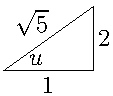
\includegraphics{fig/OQ16_4_4}
\trigtri{u}{1}{2}{\sqrt{5}}
}}
\\
&=\bigg[\frac{1}{4}\sin u \bigg]_0^{\arctan2}
\\
&=\frac{1}{4} \big( \sin(\arctan 2) - 0 \big)
= \frac{1}{2\sqrt{5}}
\end{align*}
To find $\sin(\arctan 2)$, we use the right triangle above, with angle $u=\arctan 2$. Since $\tan u=2 = \dfrac{\mbox{opp}}{\mbox{adj}}$, we label the opposite side as 2, and the adjacent side as 1. The Pythagorean Theorem tells us the hypotenuse has length $\sqrt{5}$, so \smash{$\sin u = \dfrac{\mbox{opp}}{\mbox{hyp}} = \dfrac{2}{\sqrt{5}}$.}

\item[Solution 2:]
Using our result from Question~\ref{prob:s1.9_P1},
\begin{align*}
\int_0^4 \frac{1}{{(4+x^2)}^{3/2}}\,\dee{x}&=\frac{1}{4}\left[ \dfrac x{\sqrt{x^2+4}}\right]_0^4\\
&=\frac{1}{4}\cdot \dfrac{4}{\sqrt{4^2+4}}=\frac{1}{2\sqrt{5}}
\end{align*}
\end{description}
\end{solution}
%%%%%%%%%%%%%%%%%%%


\begin{Mquestion}[M105 2013A]
Evaluate $\displaystyle\int_0^{5/2} \frac{\dee{x}}{\sqrt{25-x^2}}$.
\end{Mquestion}

\begin{hint} 
Question \ref{prob:s1.9_1} guides the way to finding the appropriate substitution.
Since the integral is definite, your final answer will be a number. Your limits of integration should be common reference angles.
\end{hint}

\begin{answer} 
$\dfrac{\pi}{6}$ 
\end{answer}

\begin{solution} 
 Make the change of variables $x=5\sin\theta$, $\dee{x}=5\cos\theta\,\dee{\theta}$. 
Since $x=0$ corresponds to $\theta=0$ and $x=\frac{5}{2}$ corresponds to
$\sin\theta=\half$ or $\theta =\frac{\pi}{6}$,
\begin{align*}
\int_0^{5/2} \frac{\dee{x}}{\sqrt{25-x^2}}
=\int_0^{\pi/6} \frac{5\cos\theta\,\dee{\theta}}{\sqrt{25-25\sin^2\theta}}
=\int_0^{\pi/6} \dee{\theta}
=\frac{\pi}{6}
\end{align*}
\end{solution}
%%%%%%%%%%%%%%%%%%%

\begin{Mquestion}[M105 2015A]
Evaluate $\displaystyle\int \frac{\dee{x}}{\sqrt{x^2+25}}$.
You may use that 
${\displaystyle\int} \sec \dee{x} = \log\big|\sec x+\tan x\big|+C$.
\end{Mquestion}

\begin{hint} 
Question \ref{prob:s1.9_1} guides the way to finding the appropriate substitution. Since you have in indefinite integral, make sure to get your answer back in terms of the original variable, $x$. Question \ref{prob:s1.9_3} gives a reliable method for this.
\end{hint}

\begin{answer} 
$\displaystyle\log\left|\sqrt{1+\frac{x^2}{25}}+\frac{x}{5}\right|+C$
\end{answer}

\begin{solution} 
Substitute $x=5\tan u$, so that $\dee{x}=5 \sec^2u\,\dee{u}$.
\begin{align*}
\int\frac{1}{\sqrt{x^2+25}}\,\dee{x}
&=\int \frac{1}{\sqrt{25\tan^2 u+25}}\,5\sec^2 u\,\dee{u}   \\[0.1in]
&=\int \frac{5\sec^2u}{5\sec u}\,\dee{u}
=\int \sec u\,\dee{u} \\[0.1in]
&= \log\big|\sec u+\tan u\big|+C
\qquad\qquad\smash{
\trigtri{u}{5}{x}{\sqrt{x^2+25}}} \\
&= \log\Big|\sqrt{1+\frac{x^2}{25}}+\frac{x}{5}\Big|+C
\end{align*}
To find $\sec u$ and $\tan u$, we have two options. One is to set up a right triangle with angle $u$ and $\tan u = \frac{x}{5}$. Then we can label the opposite side $x$ and the adjacent side 5, and use Pythagoras to find that the hypotenuse is $\sqrt{x^2+25}$.

Another option is to look back at our work a little more closely--in fact, we've already found what we're looking for. Since we used the substitution $x=5\tan u$, this gives us $\tan u = \frac{x}{5}$. In the denominator of the integrand, we simplified $\sqrt{x^2+25} = 5\sec u$, so $\sec u = \frac{1}{5}\sqrt{x^2+25} = \sqrt{1+\frac{x^2}{25}}$.

To see why we could write $\sqrt{x^2+25} =5\sec u$, as opposed to 
$\sqrt{x^2+25} =5|\sec u|$,  see
Example \eref{CLP101}{eg:INVTRIGb} in the CLP-2 text.

%As a check, we observe that the derivative of the answer
%\begin{align*}
%\diff{}{x}\left(\log\Big|\sqrt{1+\frac{x^2}{25}}+\frac{x}{5}\Big|+C\right)
%&=\frac{ \frac{\frac{2x}{25}}{2\sqrt{1+\frac{x^2}{25}}}+\frac{1}{5}}
%           {\sqrt{1+\frac{x^2}{25}}+\frac{x}{5}} \times\frac{5}{5}
%=\frac{ \frac{x}{\sqrt{x^2+25}}+1}{\sqrt{x^2+25}+x}
%=\frac{   \frac{x+\sqrt{x^2+25}}{\sqrt{x^2+25}}   }  {\sqrt{x^2+25}+x} \\
%&= \frac{1}{\sqrt{x^2+25}}
%\end{align*}
%is exactly the integrand.

\end{solution}
%%%%%%%%%%%%%%%%%%%
\begin{question}
Evaluate $\displaystyle\int\frac{x+1}{\sqrt{2x^2+4x}}
\, \dee{x}$.
\end{question}
\begin{hint}
A trig substitution is not the easiest path.
\end{hint}
\begin{answer}
$\dfrac{1}{2}\sqrt{2x^2+4x}+C$
\end{answer}
\begin{solution}
The quadratic formula underneath the square root makes us think of a trig substitution, but in the interest of developing good habits, let's check for an easier way first. If we let $u=2x^2+4x$, then $\dee{u} = (4x+4)~\dee{x}$, so $\frac{1}{4}\,\dee{u}=(x+1)\,\dee{x}$. This substitution looks easier than a trig substitution (which would start with completing the square).
\begin{align*}
\int\frac{x+1}{\sqrt{2x^2+4x}}
\, \dee{x}&=\frac{1}{4}\int \frac{1}{\sqrt{u}}\,\dee{u} = \frac{1}{2}\sqrt{u}+C = \frac{1}{2}\sqrt{2x^2+4x}+C
\end{align*}

\end{solution}
%%%%%%%%%%%%%%%%%%%



\begin{question}[2014D]
Evaluate $\displaystyle\int\frac{\dee{x}}{x^2\sqrt{x^2+16}}$.
\end{question}

\begin{hint} 
To antidifferentiate, change your trig functions into sines and cosines.
\end{hint}

\begin{answer} 
$-\displaystyle\frac{1}{16}\dfrac{\sqrt{x^2+16}}{x}+C$
\end{answer}

\begin{solution} 
Substitute $x=4\tan u$, $\dee{x}=4 \sec^2u\,\dee{u}$.
\begin{align*}
\int\frac{1}{x^2\sqrt{x^2+16}}\,\dee{x}
&=\int \frac{1}{16\tan^2 u \sqrt{16\tan^2 u+16}}\,4\sec^2 u\,\dee{u}   \\[0.1in]
&=\int \frac{\sec^2u}{16\tan^2u\sec u}\,\dee{u}
=\frac{1}{16}\int \frac{\sec u}{\tan^2u}\,\dee{u} \\[0.1in]
&= \frac{1}{16}\int\frac{\cos u}{\sin^2 u}\,\dee{u}
\end{align*}
To finish off the integral, we'll substitute $v=\sin u$, 
$\dee{v}=\cos u\,\dee{u}$.
\begin{align*}
\int\frac{1}{x^2\sqrt{x^2+16}}\,\dee{x}
&=\frac{1}{16} \int\frac{\cos u}{\sin^2 u}\,\dee{u}
= \frac{1}{16}\int\frac{\dee{v}}{v^2}
=-\frac{1}{16v} +C \\
&=-\frac{1}{16\sin u} +C 
=-\frac{1}{16}\dfrac{\sqrt{x^2+16}}{x}+C
\hskip0.5in\smash{
\trigtri{u}{4}{x}{\sqrt{x^2+16}}
%\begin{tikzpicture}
%\draw[thick] (0,0) -- (2,0) node[midway,below] {$4$};
%\draw[thick] (2,0) -- (2,1.15) node[midway,right] {$x$};
%\draw[thick] (2,1.15) -- (0,0) node[midway,above,sloped] {$\sqrt{x^2+16}$};
%\draw (1.8,0) -- (1.8,0.2) -- (2.0,0.2);
%\node (A) at (0.8,0.23) {$u$};
%\end{tikzpicture}
} 
\end{align*}
To find $\sin u$, we draw a right triangle with angle $u$ and $\tan u = \frac{x}{4}$. We label the opposite side $x$ and the adjacent side $4$, and then from Pythagoras we find that the hypotenuse has length $\sqrt{x^2+16}$. So, $\sin u = \dfrac{\sqrt{x^2+16}}{x}$.

As a check, we observe that the derivative of the answer
\begin{align*}
\diff{}{x}\left(-\frac{1}{16}\frac{\sqrt{x^2+16}}{x}+C\right)
&=\frac{1}{16}\frac{\sqrt{x^2+16}}{x^2} 
       -\frac{1}{16}\frac{x}{x\sqrt{x^2+16}}
=\frac{1}{16}\frac{(x^2+16)-x^2}{x^2\sqrt{x^2+16}} \\
&=\frac{1}{x^2\sqrt{x^2+16}}
\end{align*}
is exactly the integrand.

\end{solution}
%%%%%%%%%%%%%%%%%%%

\begin{question}[2016A]
Evaluate $\displaystyle\int \frac{\dee{x}}{x^2\sqrt{x^2-9}}$ for $x\ge 3$.
Do not include any inverse trigonometric functions in your answer.
\end{question}

\begin{hint} 
The integrand should simplify quite far after your substitution.
\end{hint}

\begin{answer} 
$\displaystyle\frac{\sqrt{x^2-9}}{9x} +C $
\end{answer}

\begin{solution} 
Substitute  $x=3\sec u$ with $0\le u<\frac{\pi}{2}$. Then $\dee{x}= 3\sec u\tan u\,\dee{u}$
and $\sqrt{x^2-9}=\sqrt{9\sec^2 u-9} =\sqrt{ 9\tan^2 u}=3\tan u$, so that
\begin{align*}
\int \frac{\dee{x}}{x^2\sqrt{x^2-9}}
&=\int \frac{3\sec u\tan u\ \dee{u}}
              {9\sec^2u\sqrt{9\tan^2u}} \\
&=\frac{1}{9}\int\frac{\dee{u}}{\sec u} \\
         &=\frac{1}{9}\int \cos u\ \dee{u} 
          =\frac{1}{9}\sin u +C.\qquad \smash{
\trigtri{u}{3}{\sqrt{x^2-9}}{x}}
\intertext{
To evaluate $\sin u$, we make a right triangle with angle $u$. Since $\sec u = \dfrac{x}{3} = \dfrac{\mbox{hyp}}{\mbox{adj}}$, we label the hypotenuse $x$ and the adjacent side $3$. Using the Pythagorean Theorem, the opposite side has length $\sqrt{x^2-9}$.
 So, $\sin u = \dfrac{\sqrt{x^2-9}}x$ and}
\int \frac{\dee{x}}{x^2\sqrt{x^2-9}} &= \frac{\sqrt{x^2-9}}{9x} +C.
\end{align*}

As a check, we observe that the derivative of the answer
\begin{align*}
\diff{}{x} \left( \frac{\sqrt{x^2-9}}{9x}+C\right)
&=-\frac{\sqrt{x^2-9}}{9x^2}     +    \frac{x}{9x\sqrt{x^2-9}}
=\frac{1}{9}\ \frac{-(x^2-9)+x^2}{x^2\sqrt{x^2-9}} \\
&=\frac{1}{x^2\sqrt{x^2-9}}
\end{align*}
is exactly the integrand. (We remark that this is the case even for $x\le -3$.)



\end{solution}
%%%%%%%%%%%%%%%%%%%


\begin{Mquestion}[2013A]
(a) Show that
$\displaystyle\int_0^{\pi/4}\cos^4\theta\ \dee{\theta}=(8+3\pi)/32$.

\medskip
\noindent (b) Evaluate
$\displaystyle\int_{-1}^1\frac{\dee{x}}{{(x^2+1)}^3}$.
\end{Mquestion}

\begin{hint} 
In part (a) you are asked to integrate an even power of $\cos x$.
For part (b) you can use a trigonometric substitution to reduce the integral
of part (b) almost to the integral of part (a).
\end{hint}

\begin{answer}
(a) We'll use the trig identity $\cos2\theta=2\cos^2\theta-1$.
It implies that
\begin{align*}
\cos^2\theta=\frac{\cos2\theta+1}{2}
\implies \cos^4\theta &=\frac{1}{4}\big[\cos^22\theta+2\cos2\theta+1\big]
=\frac{1}{4}\Big[\frac{\cos4\theta+1}{2}+2\cos2\theta+1\Big]\\
&=\frac{\cos4\theta}{8}+\frac{\cos2\theta}{2}+\frac{3}{8}
\intertext{So,}
\int_0^{\pi/4}\cos^4\theta\ \dee{\theta}
&=\int_0^{\pi/4}\Big(\frac{\cos4\theta}{8}+\frac{\cos2\theta}{2}+\frac{3}{8}\Big)
            \ \dee{\theta} \\
&=\left[\frac{\sin4\theta}{32}+\frac{\sin2\theta}{4}+\frac{3}{8}\theta\right]_0^{\pi/4}\\
&= \frac{1}{4}+\frac{3}{8}\cdot \frac{\pi}{4}\\
&=\frac{8+3\pi}{32}
\end{align*}
as required.
\\
 (b)
$\dfrac{8+3\pi}{16}$
\end{answer}

\begin{solution}
\noindent (a) 
We'll use the trig identity $\cos2\theta=2\cos^2\theta-1$.
It implies that
\begin{align*}
\cos^2\theta=\frac{\cos2\theta+1}{2}
\implies \cos^4\theta &=\frac{1}{4}\big[\cos^22\theta+2\cos2\theta+1\big]
=\frac{1}{4}\Big[\frac{\cos4\theta+1}{2}+2\cos2\theta+1\Big]\\
&=\frac{\cos4\theta}{8}+\frac{\cos2\theta}{2}+\frac{3}{8}
\intertext{So,}
\int_0^{\pi/4}\cos^4\theta\ \dee{\theta}
&=\int_0^{\pi/4}\Big(\frac{\cos4\theta}{8}+\frac{\cos2\theta}{2}+\frac{3}{8}\Big)
            \ \dee{\theta} \\
&=\left[\frac{\sin4\theta}{32}+\frac{\sin2\theta}{4}+\frac{3}{8}\theta\right]_0^{\pi/4}\\
&= \frac{1}{4}+\frac{3}{8}\cdot \frac{\pi}{4}\\
&=\frac{8+3\pi}{32}
\end{align*}
as required.

\noindent (b) We'll use the trig substitution $x=\tan\theta$,
$\dee{x}=\sec^2\theta\ \dee{\theta}$. Note that when $\theta=\pm\frac{\pi}{4}$, we have $x=\pm
1$. Also note that dividing the trig identity $\sin^2\theta+\cos^2\theta=1$ 
by $\cos^2\theta$ gives the trig identity $\tan^2\theta+1=\sec^2\theta$. So
\begin{align*}
\int_{-1}^1\frac{\dee{x}}{{(x^2+1)}^3}
&=2\int_0^1\frac{\dee{x}}{{(x^2+1)}^3}&\mbox{(even integrand)}\\
&=2\int_0^{\pi/4}\frac{\sec^2\theta\ \dee{\theta}}{{(\tan^2\theta+1)}^3}\\
&=2\int_0^{\pi/4}\frac{\sec^2\theta\ \dee{\theta}}{{(\sec^2\theta)}^3}\\
&=2\int_0^{\pi/4}\cos^4\theta\ \dee{\theta}\\
&=\frac{8+3\pi}{16}
\end{align*}
by part (a).

\end{solution}
%%%%%%%%%%%%%%%%%%%



\begin{question}
Evaluate $\displaystyle\int_{-\pi/12}^{\pi/12} \dfrac{15x^3}{(x^2+1)(9-x^2)^{5/2}}~\dee{x}$.
\end{question}
\begin{hint}
What is the symmetry of the integrand?
\end{hint}
\begin{answer}
0
\end{answer}
\begin{solution}
The integrand is an odd function, and the limits of integration are symmetric, so 
$\displaystyle\int_{-\pi/12}^{\pi/12} \dfrac{15x^3}{(x^2+1)\sqrt{9-x^2}^5}~\dee{x}=0$.
\end{solution}
%%%%%%%%%%%%%%%%%%%




\begin{question}[M121 2014A]
Evaluate ${\displaystyle\int} \sqrt{4-x^2}\,\dee{x}$.
\end{question}

\begin{hint} 
See Example \eref{CLP101}{eg:INVTRIGa} in the CLP-2 text.
\end{hint}

\begin{answer} 
$\displaystyle2\arcsin\frac{x}{2}+\frac{x}{2}\sqrt{4-x^2}+ C$
\end{answer}

\begin{solution} 
Substitute $x=2\sin u$, so that $\dee{x}=2 \cos u\,\dee{u}$.
\begin{align*}
\int \sqrt{4-x^2}\,\dee{x}
&=\int \sqrt{4-4\sin^2u}\ 2\cos u\,\dee{u}   \\
&=\int \sqrt{4\cos^2u}\ 2\cos u\,\dee{u}   \\
&=\int 4\cos^2 u\,\dee{u}
=2\int \big(1+\cos(2u)\big)\,\dee{u} \\
&= 2u +\sin(2u) + C \\
&=2u + 2\sin u\cos u + C \\
&=2\arcsin\frac{x}{2} + \frac{ x}{2}\sqrt{4-x^2} + C
\hskip0.5in\smash{
\trigtri{u}{\sqrt{4-x^2}}{x}{2}} 
\end{align*}
To see why we could write $\sqrt{4\cos^2 u} =2\cos u$, as opposed to 
$\sqrt{4\cos^2 u} =2|\cos u|$, in the third line above, see
Example \eref{CLP101}{eg trigsub2} in the CLP-2 text.

We used the substitution $x = 2\sin u$, so we know $\sin u = \frac{x}{2}$ and $u=\arcsin(\frac{x}{2})$. We have three options for finding  $\cos u$.

First, we can draw a right triangle with angle $u$. Since $\sin u = \frac{x}{2}$, we label the opposite side $x$ and the hypotenuse 2, then by the Pythagorean Theorem the adjacent side has length $\sqrt{4-x^2}$. So, $\cos u = \dfrac{\mbox{adj}}{\mbox{hyp}} = \dfrac{\sqrt{4-x^2}}{2}$.

Second, we can look back carefully at our work. We simplified $\sqrt{4-x^2} = 2\cos u$, so $\cos u = \dfrac{\sqrt{4-x^2}}{2}$.

Third, we could use the identity $\sin^2 u + \cos^2 u =1$. Then $\cos u = \pm\sqrt{1-\sin^2 u} = \pm\sqrt{1-\frac{x^2}{4}}$. Since $u = \arcsin (x/2)$, $u$ is in the range of arcsine, which means $-\frac{\pi}{2} \leq u \leq \frac{\pi}{2}$. Therefore, $\cos u \geq 0$, so $\cos u = \sqrt{1-\frac{x^2}{4}} = \frac{\sqrt{4-x^2}}{2}$.

So, 
\[\int \sqrt{4-x^2}\,\dee{x}=2u + 2\sin u\cos u + C=
2\arcsin\frac{x}{2}+x\cdot\frac{\sqrt{4-x^2}}{2}+C
\]
\end{solution}
%%%%%%%%%%%%%%%%%%%



\begin{question}[M105 2012A]
Evaluate $\displaystyle\int \frac{\sqrt{25x^2-4}}{x}\,\dee{x}$ for $x>\frac{2}{5}$.
\end{question}

\begin{hint} 
To integrate an even power of tangent, use the identity $\tan^2 x = \sec^2 x - 1$.
\end{hint}

\begin{answer} 
$\sqrt{25x^2-4}-2\arcsec\frac{5x}{2}  + C$
\end{answer}

\begin{solution} 
Substitute $x=\frac{2}{5}\sec u$ with $0< u<\frac{\pi}{2}$, so that 
$\dee{x}=\frac{2}{5} \sec u\,\tan u\,\dee{u}$ and
$\sqrt{25 x^2-4} = \sqrt{4(\sec^2u-1)} = \sqrt{4\tan^2u}=2\tan u$. Then
\begin{align*}
\int \frac{\sqrt{25x^2-4}}{x}\,\dee{x}
&=\int \frac{2\tan u}{\frac{2}{5}\sec u}\cdot\frac{2}{5}\sec u\tan u\,\dee{u} \\
&=2\int \tan^2 u\,\dee{u}
=2\int \big(\sec^2 u -1\big)\,\dee{u} \\
&= 2\tan u -2u + C \\
&=\sqrt{25x^2-4}-2\arcsec\tfrac{5x}{2}  + C
\hskip0.75in\smash{
\trigtri{u}{2}{\sqrt{25x^2-4}}{5x}} 
\end{align*}
To find $\tan u$, we draw a right triangle with angle $u$. Since $\sec u =\dfrac{5x}{2}$, we label the hypotenuse $5x$ and the adjacent side 2. Then the Pythagorean Theorem gives us the opposite side as length $\sqrt{25x^2-4}$. Then $\tan u = \dfrac{\mbox{opp}}{\mbox{adj}} = \dfrac{\sqrt{25x^2-4}}{2}$.

Alternately, we can notice that in our work, we already showed $2\tan u = \sqrt{25x^2-4}$, so $\tan u = \frac{1}{2}\sqrt{25x^2-4} .$

As a check, we observe that the derivative of the answer
\begin{align*}
\diff{}{x} \left(\sqrt{25x^2-4}-2\arcsec\frac{5x}{2}  + C\right)
&=\frac{25 x}{\sqrt{25x^2-4}} 
      - 2 \frac{\frac{5}{2}}{\left|\frac{5x}{2}\right|\sqrt{\frac{25x^2}{4}-1}} \\
&= \frac{25 x}{\sqrt{25x^2-4}}   - \frac{4}{x\sqrt{25x^2-4}}\qquad\text{since $x>0$} \\
&=  \frac{25 x^2-4}{x\sqrt{25x^2-4}} \\
&=  \frac{\sqrt{25 x^2-4}}{x}
\end{align*}
is exactly the integrand (provided $x>\frac{2}{5}$).
\end{solution}

%%%%%%%%%%%%%%%%%%%
\begin{question}
Evaluate $\displaystyle\int_{\sqrt{10}}^{\sqrt{17}} \frac{x^3}{\sqrt{x^2-1}}\, \dee{x}$.
\end{question}
\begin{hint}
A trig substitution is not the easiest path.
\end{hint}
\begin{answer}
$\dfrac{40}{3}$
\end{answer}
\begin{solution}
The integrand has a quadratic polynomial under a square root, which makes us think of trig substitutions. However, it's good practice to look for simpler methods before we jump into more complicated ones, and in this case we find something nicer than a trig substitution: the substitution $u=x^2-1$, $\dee{u}=2x\,\dee{x}$. Then $x\dee{x} = \frac{1}{2}\dee{u}$, and $x^2 ={u+1}$. When $x=\sqrt{10}$, $u=9$, and when $x=\sqrt{17}$, $u=16$.

\begin{align*}
\int_{\sqrt{10}}^{\sqrt{17}} \frac{x^3}{\sqrt{x^2-1}}\, \dee{x}&=
\int_{\sqrt{10}}^{\sqrt{17}} \frac{x^2}{\sqrt{x^2-1}}\, \cdot x\dee{x}
\\&=\frac{1}{2}
\int_{9}^{16} \frac{u+1}{\sqrt{u}}\,\dee{u}\\
&=\frac{1}{2}
\int_{9}^{16}\left(u^{1/2}+u^{-1/2}\right)\,\dee{u}
\\&=\frac{1}{2}\left[\frac{2}{3}u^{3/2} + 2u^{1/2}
\right]_{9}^{16}
\\&=\frac{1}{2}\left[\frac{2}{3}\cdot 4^3 + 2\cdot 4
-\frac{2}{3}\cdot 3^3 -2\cdot 3
\right]\\
&=\frac{40}{3}
\end{align*}
\end{solution}
%%%%%%%%%%%%%%%%%%%%%%%%%%%%

\begin{Mquestion}[M105 2014A]
Evaluate $\displaystyle\int \frac{\dee{x}}{\sqrt{3-2x-x^2}}$.
\end{Mquestion}

\begin{hint} 
Complete the square. Your final answer will have an inverse trig function in it.
\end{hint}

\begin{answer} 
$\arcsin\dfrac{x+1}{2} + C$
\end{answer}

\begin{solution} 
This integrand looks very different from those above. But it is
only slightly disguised. If we complete the square
\begin{align*}
\int \frac{\dee{x}}{\sqrt{3-2x-x^2}}
  = \int \frac{\dee{x}}{\sqrt{4-(x+1)^2}}
\end{align*}
and make the substitution $y=x+1$, $\dee{y}=\dee{x}$
\begin{align*}
\int \frac{\dee{x}}{\sqrt{3-2x-x^2}}
  = \int \frac{\dee{x}}{\sqrt{4-(x+1)^2}}
  = \int \frac{\dee{y}}{\sqrt{4-y^2}}
\end{align*}
we get a typical trig substitution integral. So, we substitute
$y=2\sin\theta$, $\dee{y}=2\cos\theta\,\dee{\theta}$ to get
\begin{align*}
\int \frac{\dee{x}}{\sqrt{3-2x-x^2}}
&= \int \frac{\dee{y}}{\sqrt{4-y^2}}
  = \int\frac{2\cos\theta\,\dee{\theta}}{\sqrt{4-4\sin^2\theta}}
  = \int\frac{2\cos\theta\,\dee{\theta}}{\sqrt{4\cos^2\theta}}\\
  &=\int\dee{\theta}
  =\theta +C
  =\arcsin\frac{y}{2} + C \\
&=\arcsin\frac{x+1}{2} + C
\end{align*}
An experienced integrator would probably substitute $x+1 = 2\sin\theta$
directly, without going through $y$. 


\end{solution}
%%%%%%%%%%%%%%%%%%%

\begin{Mquestion}
Evaluate $\displaystyle\int \dfrac{1}{(2x-3)^3\sqrt{4x^2-12x+8}}~\dee{x}$ for $x>2$.
\end{Mquestion}
\begin{hint}
To antidifferentiate even powers of   cosine, use the formula $\cos^2\theta = \frac{1}{2}(1+\cos(2\theta))$. Then, remember $\sin(2\theta)=2\sin\theta\cos\theta$.
\end{hint}
\begin{answer}
$\displaystyle\frac{1}{4}\left(\arccos\left(\frac{1}{2x-3}\right) + \frac{\sqrt{4x^2-12x+8}}{(2x-3)^2}\right)+C$, or equivalently,\\
$\displaystyle\frac{1}{4}\left(\arcsec\left({2x-3}\right) + \frac{\sqrt{4x^2-12x+8}}{(2x-3)^2}\right)+C$
\end{answer}
\begin{solution}
Completing the square, we see $4x^2-12x+8 = (2x-3)^2-1$.
\begin{align*}
\int \dfrac{1}{(2x-3)^3\sqrt{4x^2-12x+8}}~\dee{x}&=
\int \dfrac{1}{(2x-3)^3\sqrt{(2x-3)^2-1}}~\dee{x}
\intertext{As $x>2$, we have $2x-3>1$. We use the substitution $2x-3 = \sec \theta$ with $0\le\theta<\frac{\pi}{2}$. So $2\,\dee{x}=\sec\theta\tan\theta~\dee{\theta}$ and 
$\sqrt{(2x-3)^2-1}=\sqrt{\sec^2\theta-1}=\sqrt{\tan^2\theta}=\tan\theta$.}
&=\frac{1}{2}\int\frac{1}{\sec^3\theta\sqrt{\sec^2\theta-1}}\sec\theta\tan\theta~\dee{\theta}\\
&=\frac{1}{2}\int\frac{1}{\sec^3\theta\tan\theta}\sec\theta\tan\theta~\dee{\theta}
\\&=\frac{1}{2}\int\frac{1}{\sec^2\theta}~\dee{\theta}
\\&=\frac{1}{2}\int{\cos^2\theta}~\dee{\theta}
\\&=\frac{1}{4}\int{\left(1+\cos(2\theta)\right)}~\dee{\theta}
\\&=\frac14\left(\theta + \frac{1}{2}\sin(2\theta)\right)+C
\\&=\frac14\left(\theta + \sin\theta\cos\theta\right)+C
\\
\smash{\trigtri{\theta}{1}{\sqrt{4x^2-12x+8}}{2x-3}}\hspace{1cm}&=\frac{1}{4}\left(\arccos\left(\frac{1}{2x-3}\right) + \frac{\sqrt{4x^2-12x+8}}{(2x-3)^2}\right)+C
\end{align*}

Since $2x-3=\sec\theta$, we know $\cos\theta = \frac{1}{2x-3}$ and $\theta = \arccos\left(\frac{1}{2x-3}\right)$. (Equivalently, $\theta = \arcsec(2x-3)$.) To find $\sin\theta$, we draw a right triangle with adjacent side of length 1, and hypotenuse of length $2x-3$. By the Pythagorean Theorem, the opposite side has length $\sqrt{4x^2-12x+8}$.
\end{solution}
%%%%%%%%%%%%%%%%%%%




\begin{question}
Evaluate $\displaystyle\int_0^1\dfrac{x^2}{(x^2+1)^{3/2}}\dee{x}$.

You may use that  $\int \sec x\dee{x} = \log|\sec x+\tan x| +C$.
\end{question}
\begin{hint}
After substituting, use the identity $\tan^2 x = \sec^2 x - 1$ more than once.\\
 Remember $\displaystyle\int \sec x \dee{x} = \log \big|\sec x + \tan x \big|+C$.
\end{hint}
\begin{answer}
$\log(1+\sqrt{2})-\dfrac{1}{\sqrt{2}}$
\end{answer}
\begin{solution}
We use the substitution $x=\tan u$, $\dee{x}=\sec^2 u~\dee{u}$. Note $\tan 0=0$ and $\tan \frac{\pi}{4} =1$.
\begin{align*}
\displaystyle\int_0^1\dfrac{x^2}{\sqrt{x^2+1}^3}\dee{x}&=
\int_0^{\pi/4}\dfrac{\tan^2 u}{\sqrt{\tan^2 u +1}^3}\sec^2u~\dee{u}\\
&=
\int_0^{\pi/4}\dfrac{\tan^2 u}{\sqrt{\sec^2u}^3}\sec^2u~\dee{u}\\
&=
\int_0^{\pi/4}\frac{\tan^2 u}{\sec u}~\dee{u}\\&=
\int_0^{\pi/4}\frac{\sec^2 u-1}{\sec u}~\dee{u}\\&=
\int_0^{\pi/4}\big({\sec u}-\cos u\big)~\dee{u}\\
&=\Big[\log\left|\sec u + \tan u \right| - \sin u\Big]_{0}^{\pi/4}
\\
&=\left(\log\left|\sqrt{2} + 1 \right| -\frac{1}{\sqrt{2}}\right) - 
\left(\log|1+0|-0\right)\\
&=\log(1+\sqrt{2})-\frac{1}{\sqrt{2}}
\end{align*}
\end{solution}
%%%%%%%%%%%%%%%%%%%


\begin{Mquestion}\label{prob_s1.9:forpartialfractions} Evaluate $\displaystyle\int \frac{1}{(x^2+1)^2}~\dee{x}$.
\end{Mquestion}
\begin{hint}
There's no square root, but we can still make use of the substitution $x=\tan\theta$.
\end{hint}
\begin{answer}
$\displaystyle\frac{1}{2}\left(\arctan x + \frac{x}{x^2+1}\right)+C$
\end{answer}
\begin{solution}
There's no square root, but we can still make use of the substitution $x=\tan\theta$, $\dee{x} = \sec^2\theta~\dee{\theta}$.
\begin{align*}
\int \frac{1}{(x^2+1)^2}~\dee{x}&=\int\frac{1}{(\tan^2\theta+1)^2}\sec^2\theta~\dee{\theta}\\
&=\int\frac{1}{\sec^4\theta}\sec^2\theta~\dee{\theta} = \int\cos^2\theta~\dee{\theta}\\
&=\frac{1}{2}\int \big(1 + \cos(2\theta)\big)~\dee{\theta}\\
&=\frac{1}{2}\left(\theta + \frac{1}{2}\sin(2\theta)\right)+C\\
&=\frac{1}{2}\left(\theta + \sin\theta\cos\theta\right)+C\\
\smash{\trigtri{\theta}{1}{x}{\sqrt{x^2+1}}}\hspace{1cm}&=\frac{1}{2}\left(\arctan x + \frac{x}{x^2+1}\right)+C
\end{align*}
Since $x = \tan\theta$, we can draw a right triangle with angle $\theta$, opposite side $x$, and adjacent side $1$. Then by the Pythagorean Theorem, its hypotenuse has length $\sqrt{x^2+1}$, which allows us to find $\sin\theta$ and $\cos\theta$.
\end{solution}


%%%%%%%%%%%%%%%%%%
\subsection*{\Application}
%%%%%%%%%%%%%%%%%%



\begin{question}
Evaluate $\displaystyle\int \dfrac{x^2}{\sqrt{x^2-2x+2}}~\dee{x}$. \\
You may assume without proof that $\displaystyle\int \sec^3 \theta~\dee{\theta} = \frac{1}{2}\sec\theta\tan\theta + \frac{1}{2}\log|\sec\theta+\tan\theta|+C$.
\end{question}
\begin{hint}
You'll probably want to use the identity $\tan^2\theta+1=\sec^2\theta$ more than once.
\end{hint}
\begin{answer}
$\dfrac{3+x}{2}\sqrt{x^2-2x+2}+ \dfrac{1}{2}\log\left|\sqrt{x^2-2x+2}+x-1\right|+C$
\end{answer}
\begin{solution}
We complete the square to find $x^2-2x+2 = (x-1)^2+1$.
\begin{align*}
\int \dfrac{x^2}{\sqrt{x^2-2x+2}}~\dee{x}&=
\int \dfrac{x^2}{\sqrt{(x-1)^2+1}}~\dee{x}
\intertext{We use the substitution $x-1=\tan\theta$,  which implies $\dee{x}=\sec^2\theta~\dee{\theta}$ and $x=\tan\theta+1$}
&=\int \dfrac{(\tan\theta+1)^2}{\sqrt{(\tan\theta)^2+1}}~\sec^2\theta~\dee{\theta}\\
&=\int\frac{\textcolor{red}{\tan^2\theta}+2\tan\theta+\textcolor{red}1}{\sec\theta}\sec^2\theta~\dee{\theta}\\
&=\int(\textcolor{red}{\sec^2\theta}+2\tan\theta)\sec\theta~\dee{\theta}\\
&=\int\big( \sec^3\theta+2\tan\theta\sec\theta\big)~\dee{\theta}
\hspace{2cm}\smash{\trigtri{\theta}{1}{x-1}{\sqrt{x^2-2x+2}}}\\
&=\frac{1}{2}\sec\theta\tan\theta + \frac{1}{2}\log|\sec\theta+\tan\theta|+2\sec\theta+C\\
&=\frac{1}{2}\sqrt{x^2-2x+2}(x-1) + \frac{1}{2}\log\left|\sqrt{x^2-2x+2}+x-1\right|\\
&\hskip 1in+2\sqrt{x^2-2x+2}+C\\
&=\frac{3+x}{2}\sqrt{x^2-2x+2}+ \frac{1}{2}\log\left|\sqrt{x^2-2x+2}+x-1\right|+C
\end{align*}
To see why we could write $\sqrt{(\tan\theta)^2+25} =\sec\theta$, as opposed to 
$\sqrt{(\tan\theta)^2+25} =|\sec\theta|$,  see
Example \eref{CLP101}{eg:INVTRIGb} in the CLP-2 text.

From our substitution, we know $\tan\theta = x-1$. To find $\sec\theta$, we can notice that in our work we already simplified $\sqrt{x^2-2x+1}=\sec\theta$. Alternately, we can draw a right triangle with angle $\theta$, opposite side $x-1$, adjacent side $1$, and use the Pythagorean Theorem to find the hypotenuse.
\end{solution}
%%%%%%%%%%%%%%%%%%%

\begin{Mquestion}
Evaluate $\displaystyle\int \dfrac{1}{\sqrt{3x^2+5x}}~\dee{x}$.

You may use that  $\int \sec x\dee{x} = \log|\sec x+\tan x| +C$.
\end{Mquestion}
\begin{hint}
Complete the square --- refer to Question~\ref{prob_21.9:complete} if you want a refresher. The constants aren't pretty, but don't let them scare you.
\end{hint}
\begin{answer}
$\displaystyle\frac{1}{\sqrt{3}}\log\left| \left(\frac{6}{5}x+1\right)+\frac{2}{5}\sqrt{9x^2+15x} \right|+C$
\end{answer}
\begin{solution}
First, we complete the square. The constants aren't integers, but we can still use the same method as in Question~\ref{prob_21.9:complete}.
The quadratic function under the square root is $3x^2+5x$. We match the non-constant terms to those of a perfect square.
\begin{align*}
(ax+b)^2&=a^2x^2+2abx+b^2\\
\textcolor{red}{3x^2}+\textcolor{blue}{5x}&=\textcolor{red}{a^2x^2} + \textcolor{blue}{2abx} +b^2 + c \quad\mbox{for some constant $c$}
\end{align*}
\begin{itemize}
\item \textcolor{red}{Looking at the leading term tells us $a=\sqrt{3}$. }
\item \textcolor{blue}{Then the second term tells us $5=2ab=2\sqrt{3}b$, so $b=\frac{5}{2\sqrt3}$.}
\item Finally, the constant terms give us $0=b^2+c=\frac{25}{12}+c$, so $c=-\frac{25}{12}$.
\end{itemize}

So, $3x^2+5x=\left(\sqrt{3}x+\frac{5}{2\sqrt{3}}\right)^2-\frac{25}{12}$.
\begin{align*}
\int \dfrac{1}{\sqrt{3x^2+5x}}~\dee{x}&=\int \dfrac{1}{\sqrt{\left(\sqrt{3}x+\frac{5}{2\sqrt3}\right)^2-\frac{25}{12}}}~\dee{x}
\intertext{We use the substitution $\sqrt{3}x + \frac{5}{2\sqrt3}=\frac{5}{2\sqrt{3}}\sec\theta$, which leads to $\sqrt{3}\dee{x} = \frac{5}{2\sqrt{3}}\sec\theta\tan\theta~\dee{\theta}$, i.e. $\dee{x} = \frac{5}{6}\sec\theta\tan\theta~\dee{\theta}$.}
&=\int\frac{1}{\sqrt{\left(\frac{5}{2\sqrt3}\sec\theta\right)^2-\frac{25}{12}}}\cdot\frac{5}{6}\sec\theta\tan\theta~\dee{\theta}\\
&=\int\frac{1}{\sqrt{\frac{25}{12}\sec^2\theta-\frac{25}{12}}}\cdot\frac{5}{6}\sec\theta\tan\theta~\dee{\theta}\\
&=\int\frac{1}{\sqrt{\frac{25}{12}\tan^2\theta}}\cdot\frac{5}{6}\sec\theta\tan\theta~\dee{\theta}\\
&=\int\frac{1}{{\frac{5}{2\sqrt{3}}\tan\theta}}\cdot\frac{5}{6}\sec\theta\tan\theta~\dee{\theta}\\
&=\frac{1}{\sqrt3}\int\sec\theta~\dee{\theta}\\
&=\frac{1}{\sqrt3}\log\left|\sec\theta+\tan\theta\right|+C\\
\smash{\trigtri{\theta}{5}{2\sqrt{9x^2+15x}}{6x+5}}
\hspace{1.5cm}
&=\frac{1}{\sqrt3}\log\left| \left(\frac{6}{5}x+1\right)+\frac{2}{5}\sqrt{9x^2+15x} \right|+C
\end{align*}
Since we used the substitution $\sqrt3x+\frac{5}{2\sqrt{3}}=\frac{5}{2\sqrt3}\sec\theta$, we have $\sec\theta = \frac{6}{5}x+1 = \frac{6x+5}{5}$. To find $\tan\theta$ in terms of $x$, we have two options. We can make a right triangle with angle $\theta$, hypotenuse $6x+5$, and adjacent side $5$, then use the Pythagorean Theorem to find the opposite side. Or, we can look through our work and see that $\sqrt{3x^2+5}=\frac{5}{2\sqrt3}\tan\theta$, so $\tan\theta = \frac{2\sqrt3}{5}\sqrt{3x^2+5}=\frac{2}{5}\sqrt{9x^2+15}$.


As a check, we observe that the derivative of the answer
\begin{align*}
&\diff{}{x}\left(
\frac{1}{\sqrt3}\log\left| \left(\frac{6}{5}x+1\right)+\frac{2}{5}\sqrt{9x^2+15x} \right| + C\right)
=\frac{1}{\sqrt3}\ \frac{\frac{6}{5} +\frac{1}{5} \frac{18x+15}{\sqrt{9x^2+15 x}}}
              { \left(\frac{6}{5}x+1\right)+\frac{2}{5}\sqrt{9x^2+15x}} \\
&\hskip0.5in=\frac{1}{\sqrt3}\ \frac{6 + 3\frac{6x+5}{\sqrt{9x^2+15 x}}}
              { \left(6x+5\right)+ 2\sqrt{9x^2+15x}} 
=\sqrt3\ \frac{2 + \frac{6x+5}{\sqrt{9x^2+15 x}}}
              { \left(6x+5\right)+ 2\sqrt{9x^2+15x}} 
=\frac{\sqrt{3}}{\sqrt{9x^2+15 x}} \\
&\hskip0.5in=\frac{1}{\sqrt{3x^2+5 x}}
\end{align*}
is exactly the integrand.

Remark: in applications, often the numbers involved are messier than they are in textbooks. The ideas of this problem are similar to other problems in this section, but it's good practice to apply them in a slightly messy context.
\end{solution}
%%%%%%%%%%%%%%%%%%%




\begin{question}
Evaluate $\displaystyle\int\dfrac{(1+x^2)^{3/2}}{x}\dee{x}$. You may use the fact that $\displaystyle\int \csc 
\theta~\dee{\theta}=\log|\cot \theta - \csc \theta|+C$.
\end{question}
\begin{hint}
After substituting, use the identity $\sec^2 u = \tan^2 u +1$. It might help to break the integral into a few pieces.
\end{hint}
\begin{answer}
$\dfrac{1}{3}\sqrt{1+x^2}(4+x^2)+\log\left|\dfrac{1-\sqrt{1+x^2}}{x} \right|+C$
\end{answer}
\begin{solution}
We use the substitution $x=\tan u$, $\dee{x}=\sec^2 u~\dee{u}$.
\begin{align*}
\int\dfrac{\sqrt{1+x^2}^3}{x}\dee{x}&=\int\frac{\sqrt{1+\tan^2 u}^3}{\tan u}\sec^2 u~\dee{u}
\\&=\int\frac{\sec^3u}{\tan u}\sec^2 u~\dee{u}
\\&=\int\frac{(\sec^2u)^2}{\tan u}\sec u~\dee{u}
\\&=\int\frac{(\tan^2u+1)^2}{\tan u}\sec u~\dee{u}
\\&=\int\frac{\tan^4u+2\tan^2 u + 1}{\tan u}\sec u~\dee{u}
\\&=\int \tan^3 u \sec u ~\dee{u} + \int 2\sec u \tan u~\dee u + \int \frac{\sec u}{\tan u}~\dee{u}
\intertext{For the first integral, we use the substitution $w=\sec u$. The second is the antiderivative of $2\sec u$. The third we simplify as $\frac{\sec u}{\tan u} = \frac{1}{\cos u}\cdot \frac{\cos u}{\sin u} = \csc u$~.}
&=\int\bigg((\sec^2 u -1)\sec u \tan u\bigg)~\dee{u} + 2\sec u + \log|\cot u - \csc u |+C\\
&=\int (w^2-1)~\dee{w}+2\sec u + \log|\cot u - \csc u|+C\\
&=\frac{1}{3}w^3-w+2\sec u + \log|\cot u - \csc u|+C\\
&=\frac{1}{3}\sec^3u-\sec u+2\sec u + \log|\cot u - \csc u|+C
\\
\smash{\trigtri{u}{1}{x}{\sqrt{1+x^2}}} \qquad &=\frac{1}{3}\sec^3u+\sec u + \log|\cot u - \csc u|+C
\intertext{We began with the substitution $x=\tan u$. Then $\cot u = \frac{1}{x}$. To find $\csc u$ and $\sec u$, we draw a right triangle with angle $u$, opposite side $x$, and adjacent side $1$. The Pythagorean Theorem gives us the hypotenuse.}
&=\frac{1}{3}\sqrt{1+x^2}^3+\sqrt{1+x^2}+\log\left| \frac{1}{x}-\frac{\sqrt{1+x^2}}{x} \right|+C
\\&=\frac{1}{3}\sqrt{1+x^2}(4+x^2)+\log\left|\frac{1-\sqrt{1+x^2}}{x} \right|+C
\end{align*}
\end{solution}


%%%%%%%%%%%%%%%%%%%

\begin{Mquestion}
Below is the graph of the ellipse $\left(\frac{x}{4}\right)^2+\left(\frac{y}{2}\right)^2=1$. Find the area of the shaded region using the ideas from this section.
\begin{center}
\begin{tikzpicture}
\draw (0,0) node[shape=ellipse, minimum width=8cm, minimum height=4cm, draw]{};
\fill[fill=blue, fill opacity=0.2] plot[domain=-1:1, samples=100]({4*sqrt(1-\x*\x/4)},\x)--
plot[domain=1:-1, samples=100]({-4*sqrt(1-\x*\x/4)},\x)--cycle;
\YEaxis{4.5}{2.25}
\YEycoord{-1}{-1}
\YEycoord{1}{1}
\end{tikzpicture}
\end{center}
\end{Mquestion}
\begin{hint}
Make use of symmetry, and integrate with respect to $y$ (rather than $x$). The limits of integration should be reference angles.
\end{hint}
\begin{answer}
$\dfrac{8\pi}{3}+4\sqrt{3}$
\end{answer}
\begin{solution}
The half of the ellipse to the right of the $y$-axis is given by the equation
\begin{align*}
x=f(y)&=4\sqrt{1-\left(\frac{y}{2}\right)^2}
\intertext{The area we want is the twice the area between the right-hand side of the curve and the $y$-axis, from $y=-1$ to $y=1$. In other words,}
\mbox{Area}&=2\int_{-1}^1 4\sqrt{1-\left(\frac{y}{2}\right)^2}~\dee{y}
\intertext{Making use of symmetry,}
&=16\int_{0}^1 \sqrt{1-\left(\frac{y}{2}\right)^2}~\dee{y}
\intertext{We use the substitution $\frac{y}{2} = \sin \theta$, $\frac{1}{2}\dee{y}=\cos\theta~\dee{\theta}$. Notice $\sin \frac{\pi}{6} = \frac{1}{2}$ and $\sin 0 =0$.}
&=16\int_{0}^{\pi/6} \sqrt{1-\left(\sin\theta\right)^2}\ \ 2\cos\theta~\dee{\theta}
\\&=32\int_{0}^{\pi/6} \sqrt{\cos^2\theta}~\cos\theta~\dee{\theta}
\\&=32\int_{0}^{\pi/6}\cos^2\theta~\dee{\theta}
\\&=16\int_{0}^{\pi/6}\left(1+\cos(2\theta)\right)~\dee{\theta}
\\&=16\left[\theta +\frac{1}{2}\sin(2\theta)\right]_{0}^{\pi/6}\\
&=16\left(\frac{\pi}{6}+\frac{1}{2}\cdot \frac{\sqrt{3}}{2}
\right)\\
&=\frac{8\pi}{3}+4\sqrt{3}
\end{align*}

Remark: we also investigated areas of ellipses in Question~\ref{prob_s1.2:ellipsearea}, Section 1.2.
\end{solution}
%%%%%%%%%%%%%%%%%%%


\begin{question}
Let $f(x) = \dfrac{|x|}{\sqrt[4]{1-x^2}}$, and let $R$ be the region between $f(x)$ and the $x$-axis over the interval $[-\frac{1}{2},\frac{1}{2}]$.
\begin{enumerate}[(a)]
\item Find the area of $R$.
\item Find the volume of the solid formed by rotating $R$ about the $x$-axis.
\end{enumerate}
\end{question}
\begin{hint}
Use the symmetry of the function to re-write your integrals without an absolute value.
\end{hint}
\begin{answer}
Area: $\dfrac{4}{3} - \sqrt[4]{\dfrac{4}{3}}$\qquad
Volume: $\dfrac{\pi^2}{6} - \dfrac{\sqrt{3}\pi}{4}$
\end{answer}
\begin{solution}
Note that $f(x)$ is an even function, nonnegative over its entire domain.\\
\noindent (a) To find the area of $R$, we evaluate
\begin{align*}
\mbox{Area}&=\int _{-1/2}^{1/2} \dfrac{|x|}{\sqrt[4]{1-x^2}}~\dee{x} = 
2\int _{0}^{1/2} \dfrac{x}{\sqrt[4]{1-x^2}}~\dee{x}
\intertext{We use the substitution $u=1-x^2$, $\dee{u}=-2x~\dee{x}$.}
&=-\int_{1}^{3/4} \frac{1}{u^{1/4}}~\dee{u}\\
&=-\left[\frac{4}{3}u^{3/4}\right]_1^{3/4} = -\frac{4}{3}\left(\left(\frac{3}{4}\right)^{3/4}-1\right)\\
&=\frac{4}{3} - \sqrt[4]{\frac{4}{3}}
\end{align*}
\noindent (b) We slice the solid of rotation into circular disks of width $\dee{x}$ and radius $\dfrac{|x|}{\sqrt[4]{1-x^2}}$.
\begin{align*}
\mbox{Volume}&=\int_{-1/2}^{1/2} \pi\left(\dfrac{|x|}{\sqrt[4]{1-x^2}}\right)^2~\dee{x}\\
&=2\pi\int_{0}^{1/2} \dfrac{x^2}{\sqrt{1-x^2}}~\dee{x}
\intertext{We use the substitution $x=\sin \theta$, $\dee{x} = \cos\theta~\dee{\theta}$, so $\sqrt{1-x^2} = \sqrt{1-\sin^2\theta}=\cos \theta$. Note $\sin 0 =0$ and $\sin\frac{\pi}{6}=\frac{1}{2}.$}
&=2\pi\int_{0}^{\pi/6} \frac{\sin^2 \theta}{\cos \theta}\cos \theta~\dee{\theta}
\\&=2\pi\int_{0}^{\pi/6} \sin^2 \theta~\dee{\theta}
\\&=\pi\int_{0}^{\pi/6}\big(1- \cos(2 \theta)\big)~\dee{\theta}\\
&=\pi\left[\theta - \frac{1}{2}\sin(2\theta)\right]_0^{\pi/6}\\
&=\pi\left(\frac{\pi}{6} - \frac{1}{2}\cdot \frac{\sqrt{3}}{2}\right)\\
&=\frac{\pi^2}{6} - \frac{\sqrt{3}\pi}{4}
\end{align*}
\end{solution}
%%%%%%%%%%%%%%%%%%%


\begin{question}\label{prob_s1.9:sqrt1ex}
Evaluate $\displaystyle\int \sqrt{1+e^x}~\dee{x}$.
You may use the antiderivative $\displaystyle\int \csc \theta \dee{\theta} = \log|\cot \theta - \csc \theta|+C$.
\end{question}
\begin{hint} Think of $e^x$ as $\left(e^{x/2}\right)^2$, and use a trig substitution. Then, use the identity $\sec^2 \theta = \tan^2 \theta +1$.
\end{hint}
\begin{answer}
$2\sqrt{1+e^x}+2\log\left| 1-\sqrt{1+e^x} \right|-x+C
$
\end{answer}
\begin{solution}
If we think of $e^x$ as $\left(e^{x/2}\right)^2$, the function under the square root suggests the substitution $e^{x/2}=\tan \theta$. Then $\frac{1}{2}e^{x/2}~\dee{x}=\sec^2\theta~\dee{\theta}$, so $\dee{x} = \frac{2}{e^{x/2}}\sec^2\theta~\dee{\theta} = \frac{2}{\tan\theta}\sec\theta~\dee{\theta}$.
\begin{align*}
\int \sqrt{1+e^x}~\dee{x}&=\int\frac{2\sqrt{1+\tan^2 \theta}}{\tan\theta}\sec^2\theta~\dee{\theta}\\
&=2\int \frac{\sec^3\theta}{\tan\theta}~\dee{\theta}\\
&=2\int \frac{\sec\theta(\tan^2\theta+1)}{\tan\theta}~\dee{\theta}\\
&=2\int \left(\sec\theta \tan\theta + \frac{\sec \theta}{\tan\theta}\right)~\dee{\theta}\\
&=2\int\big( \sec\theta \tan\theta + \csc\theta\big)~\dee{\theta}\\
\smash{\trigtri{\theta}{1}{e^{x/2}}{\sqrt{1+e^x}}}\hspace{2cm}&=2\sec\theta + 2\log|\cot\theta-\csc\theta|+C\\
&=2\sqrt{1+e^x}+2\log\left| \frac{1}{e^{x/2}} - \frac{\sqrt{1+e^x}}{e^{x/2}} \right|+C\\
&=2\sqrt{1+e^x}+2\log\left| 1-\sqrt{1+e^x} \right|-2\log(e^{x/2})+C
\\&=2\sqrt{1+e^x}+2\log\left| 1-\sqrt{1+e^x} \right|-x+C
\end{align*}
We used the substitution $e^{x/2}=\tan\theta$, so $\cot\theta = \frac{1}{e^{x/2}}$. To find $\sec \theta$ and $\csc\theta$, we draw a right triangle with opposite side $e^{x/2}$ and adjacent side 1. They by the Pythagorean Theorem, the hypotenuse has length $\sqrt{1+e^x}$.

Remark: if we use the substitution $u=\sqrt{1+e^x}$, then we can change the integral to $\displaystyle\int \dfrac{2u^2}{u^2-1}~\dee{u}$. We can integrate this using the method of partial fractions, which we'll learn in the next section. You can explore this option in Question~\ref{prob_s1.10:sqrt1ex}, Section 1.10.
\end{solution}
%%%%%%%%%%%%%%%%%%%

\begin{Mquestion}
Consider the following work.
\color{blue}
\begin{align*}
\int \frac{1}{1-x^2}~\dee{x}&=\int\dfrac{1}{1-\sin^2 \theta}\cos\theta~\dee{\theta}&\mbox{using } x=\sin\theta,\quad \dee{x}=\cos\theta~\dee{\theta}\\
&=\int \frac{\cos \theta}{\cos^2 \theta}~\dee\theta\\
&=\int \sec \theta~\dee{\theta}\\
&=\log|\sec \theta + \tan \theta| +C & \mbox{Example~\eref{CLP101}{eg:TRGINTopta} in the CLP-2 text}\\
&=\log\left | 
\dfrac{1}{\sqrt{1-x^2}}+\dfrac{x}{\sqrt{1-x^2}}
\right| +C\\
\smash{\trigtri{\theta}{\sqrt{1-x^2}}{x}{1}}\qquad&=\log\left | 
\dfrac{1+x}{\sqrt{1-x^2}}
\right| +C
\end{align*}
\color{black}
\begin{enumerate}[(a)]
\item Differentiate $\log\left|  \dfrac{1+x}{\sqrt{1-x^2}}\right|$.
\item True or false: $\displaystyle\int_{2}^{3} \frac{1}{1-x^2}~\dee{x} =
\left[\log\left|  \dfrac{1+x}{\sqrt{1-x^2}}\right|\right]_{x=2}^{x=3}$
\item Was the work in the question correct? Explain.
\end{enumerate}
\end{Mquestion}
\begin{hint}
\begin{enumerate}[(a)]
\item Use logarithm rules to simplify first.
\item Think about domains.
\item What went wrong in part (b)? At what point in the work was that problem introduced?\\
There is a subtle but important point mentioned in the introductory text to Section~\eref{CLP101}{sec trigsub} of the CLP-2 text that may help you make sense of things.
\end{enumerate}
\end{hint}
\begin{answer}

\begin{enumerate}[(a)]
\item $\dfrac{1}{1-x^2}$
\item False
\item The work in the question is not correct. The most salient problem is that when we make the substitution $x=\sin\theta$, we restrict the possible values of $x$ to $[-1,1]$, since this is the range of the sine function. However, the original integral had no such restriction.

How can we be sure we avoid this problem in the future? In the introductory text to Section~\eref{CLP101}{sec trigsub} (before Example~\eref{CLP101}{eg first trigsub}), the 
CLP-2 text tells us that we are allowed to write our old variable as a function of a new variable (say $x=s(u)$) \emph{as long as that function is invertible to recover our original variable} $x$. There is one very obvious reason why invertibility is necessary: after we antidifferentiate using our new variable $u$, we need to get it back in terms of our original variable, so we need to be able to recover $x$. Moreover, invertibility  reconciles  potential problems with domains: if an inverse function $u=s^{-1}(x)$ exists, then for any $x$, there exists a $u$ with $s(u)=x$. (This was not the case in the work for the question, because we chose $x=\sin \theta$, but if $x=2$, there is no corresponding $\theta$. Note, however, that $x=\sin\theta$ is invertible over $[-1,1]$,  so the work is correct if we restrict $x$ to those values.)

\end{enumerate}

\end{answer}
\begin{solution}
\begin{enumerate}[(a)]
\item We can save ourselves some trouble by applying logarithm rules before we differentiate.
\begin{align*}
\log\left|  \dfrac{1+x}{\sqrt{1-x^2}}\right|&=\log|1+x| - \log|\sqrt{1-x^2}|\\
&=\log|1+x| - \frac{1}{2}\log|1-x^2|\\
&=\log|1+x| - \frac{1}{2}\log|(1+x)(1-x)|\\
&=\log|1+x| - \frac{1}{2}\log|1+x|- \frac{1}{2}\log|1-x|\\
\diff{}{x}\left\{\log\left|  \dfrac{1+x}{\sqrt{1-x^2}}\right|\right\}&=
\diff{}{x}\left\{\log|1+x| - \frac{1}{2}\log|1+x|- \frac{1}{2}\log|1-x|\right\}\\
&=\frac{1}{1+x} -  \frac{1/2}{1+x}+ \frac{1/2}{1-x}\\
&=  \frac{1/2}{1+x}+ \frac{1/2}{1-x}\\
&=\frac{1}{1-x^2}
\end{align*}
Notice this is the integrand from our work in blue.
\item False: $\displaystyle\int_{2}^{3} \frac{1}{1-x^2}~\dee{x}$ is a number, because it is the area under a finite portion of a continuous curve. (We note that the integrand is continuous over the interval $[2,3]$, although it is not continuous everywhere.) However, 
$\left[\log\left|  \dfrac{1+x}{\sqrt{1-x^2}}\right|\right]_{x=2}^{x=3}$ is not defined, since the denominator takes the square root of a negative number. So, these two expressions are not the same.
\item The work in the question is not correct. The most salient problem is that when we make the substitution $x=\sin\theta$, we restrict the possible values of $x$ to $[-1,1]$, since this is the range of the sine function. However, the original integral had no such restriction.

How can we be sure we avoid this problem in the future? In the introductory text to Section~\eref{CLP101}{sec trigsub} (before Example~\eref{CLP101}{eg first trigsub}), the 
CLP-2 text tells us that we are allowed to write our old variable as a function of a new variable (say $x=s(u)$) \emph{as long as that function is invertible to recover our original variable} $x$. There is one very obvious reason why invertibility is necessary: after we antidifferentiate using our new variable $u$, we need to get it back in terms of our original variable, so we need to be able to recover $x$. Moreover, invertibility  reconciles  potential problems with domains: if an inverse function $u=s^{-1}(x)$ exists, then for any $x$, there exists a $u$ with $s(u)=x$. (This was not the case in the work for the question, because we chose $x=\sin \theta$, but if $x=2$, there is no corresponding $\theta$. Note, however, that $x=\sin\theta$ is invertible over $[-1,1]$,  so the work is correct if we restrict $x$ to those values.)

Remark: in the next section, you will learn to use partial fractions to find $\displaystyle\int \dfrac{1}{1-x^2}~\dee{x} = \log|1+x|-\dfrac{1}{2}\log|1-x|$. When $-1<x<1$, this is equivalent to $\log\left| \dfrac{1+x}{\sqrt{1-x^2}}\right|$.
\end{enumerate}

\end{solution}
%%%%%%%%%%%%%%%%%%%




\begin{question}
\begin{enumerate}[(a)]
\item Suppose we are evaluating an integral that contains the term $\sqrt{a^2-x^2}$, where $a$ is a positive constant, and we use the substitution $x=a\sin u$ (with inverse $u = \arcsin(x/a)$), so that
\[\sqrt{a^2-x^2} = \sqrt{a^2\cos^2u}= |a\cos u|\]
Under what circumstances is $|a\cos u|\neq a\cos u$?
\item Suppose we are evaluating an integral that contains the term $\sqrt{a^2+x^2}$, where $a$ is a positive constant, and we use the substitution $x=a\tan u$ (with inverse $u = \arctan(x/a)$), so that
\[\sqrt{a^2+x^2} = \sqrt{a^2\sec^2u}= |a\sec u|\]
Under what circumstances is $|a\sec u|\neq a\sec u$?
\item Suppose we are evaluating an integral that contains the term $\sqrt{x^2-a^2}$, where $a$ is a positive constant, and we use the substitution $x=a\sec u$ (with inverse $u = \arcsec(x/a)=\arccos(a/x)$), so that
\[\sqrt{x^2-a^2} = \sqrt{a^2\tan^2u}= |a\tan u|\]
Under what circumstances is $|a\tan u|\neq a\tan u$?

\end{enumerate}
\end{question}
\begin{hint}
Consider the ranges of the inverse trigonometric functions. For (c), also consider the domain of $\sqrt{x^2-a^2}$.
\end{hint}
\begin{answer}
(a), (b): None. \qquad (c): $x< -a$
\end{answer}
\begin{solution}
Remember that for any value $X$, 
\[|X| = \left\{\begin{array}{rl}
X&\mbox{if }X \ge 0\\
-X&\mbox{if }X \le 0
\end{array}\right.\]
So, $|X| \neq X$ precisely when $X<0$.

(a) The range of arcsine is $\big[-\frac{\pi}{2},\frac{\pi}{2}\big]$. So, since $u=\arcsin(x/a)$, $u$ is in the range $\big[-\frac{\pi}{2},\frac{\pi}{2}\big]$. Therefore $\cos u \geq 0$. Since $a$ is positive, $a\cos u \ge 0$, so $a\cos u = |a\cos u|$. That is,
\[\sqrt{a^2-x^2}=|a\cos u|=a\cos u\]
all the time.

(b) The range of arctangent is $\big(-\frac{\pi}{2},\frac{\pi}{2}\big)$. So, since $u=\arctan(x/a)$, $u$ is in the range $\big(-\frac{\pi}{2},\frac{\pi}{2}\big)$. Therefore $\sec u = \frac{1}{\cos u} >0 $. Since $a$ is positive, $a\sec u > 0$, so $a\sec u = |a\sec u|$.That is,
\[\sqrt{a^2+x^2}=|a\sec u|=a\sec u\]
all the time.

(c) The range of arccosine is $\big[0,\pi \big]$. So, since $u=\arcsec(x/a) = \arccos(a/x)$, $u$ is in the range $\big[0,\pi\big]$. (Actually, it's in the range $[0,\frac{\pi}{2}) \cup (\frac{\pi}{2},\pi]$, since secant is undefined at $\pi/2$.) If $|a\tan u| \neq a\tan u$, then $\tan u <0$, which happens when $u$ is in the range $\big (\frac{\pi}{2},\pi)$. This is the same range over which $-1<\cos u <0$, and so $-1<\frac{a}{x}<0$. 
Since $\frac{a}{x}<0$, $a$ and $x$ have different signs, so $x<0$.  Then since $-1<\frac{a}{x}$, also $x<-a$.

So,
\[\sqrt{x^2-a^2} = |a\tan u| = -a\tan u \neq a\tan u\]
happens precisely when  when $x< -a$. 
\end{solution}
%%%%%%%%%%%%%%%%%%%

\section{Partial Fractions}
%
% Copyright 2018 Joel Feldman, Andrew Rechnitzer and Elyse Yeager.
% This work is licensed under a Creative Commons Attribution-NonCommercial-ShareAlike 4.0 International License.
% https://creativecommons.org/licenses/by-nc-sa/4.0/
%
\questionheader{ex:s1.10}

\noindent
Recall that we are using $\log x$ to denote the logarithm of $x$ with
base $e$. In other courses it is often denoted $\ln x$.


%%%%%%%%%%%%%%%%%%
\subsection*{\Conceptual}
%%%%%%%%%%%%%%%%%%
\begin{Mquestion}
Below are the graphs of four different quadratic functions. For each quadratic function, decide whether it is: (i) irreducible, (ii) the product of two distinct linear factors, or (iii) the product of a repeated linear factor (and possibly a constant).

\begin{tikzpicture}[scale=0.5]
\YEaxis{3}{3}
\draw[thick] plot[domain=-2.8:2.8](\x,{\x*\x/3});
\draw (-1.5,-3) node[below]{(a)};
\end{tikzpicture}\hfill
\begin{tikzpicture}[scale=0.5]
\YEaxis{3}{3}
\draw[thick] plot[domain=-5:5](\x/2,{\x*\x/5-2});
\draw (-1.5,-3) node[below]{(b)};
\end{tikzpicture}\hfill
\begin{tikzpicture}[scale=0.5]
\YEaxis{3}{3}
\draw[thick] plot[domain=-5:5](\x/10+1.5,{2-\x*\x/5});
\draw (-1.5,-3) node[below]{(c)};
\end{tikzpicture}\hfill
\begin{tikzpicture}[scale=0.5]
\YEaxis{3}{3}
\draw[thick] plot[domain=-2:2](\x,{-1-\x*\x/2});
\draw (-1.5,-3) node[below]{(d)};
\end{tikzpicture}


\end{Mquestion}
\begin{hint}
If a quadratic function can be factored as $(ax+b)(cx+d)$ for some constants $ a,b,c,d$, then it has roots $-\frac{b}{a}$ and $-\frac{d}{c}$.
\end{hint}
\begin{answer}
(a) (iii) \qquad (b) (ii) \qquad (c) (ii) \qquad (d) (i)
\end{answer}
\begin{solution}
If a quadratic function can be factored as $(ax+b)(cx+d)$ for some constants $ a,b,c,d$, then it has roots $-\frac{b}{a}$ and $-\frac{d}{c}$. So, if a quadratic function has no roots, it is irreducible: this is the case for the function in graph (d).

If a quadratic function has  two different roots, then $(ax+b) \neq \alpha(cx+d)$ for any constant $\alpha$. That is, the quadratic function is the product of distinct linear factors. This is the case for the functions graphed in (b) and (c), since these each have two distinct places where they cross the $x$-axis.

Finally, if a quadratic function has precisely one root, then $\frac{b}{a}=\frac{d}{c}$, so:
\begin{align*}
(ax+b)(cx+d)&=a(x+\tfrac{b}{a})(cx+d) = a(x+\tfrac{d}{c})(cx+d) = \tfrac{a}{c}(cx+d)(cx+d)
\end{align*}
That is, the quadratic function is the product of a repeated linear factor, and  a constant $\frac{a}{c}$ (which might simply be $\frac{a}{c}=1$).
\end{solution}
%%%%%%%%%%%%%%%%%%%


\begin{Mquestion}[2016Q4]
Write out the \textbf{general form} of the partial-fractions
decomposition of
$
\displaystyle\frac{x^3+3}{(x^2-1)^2(x^2+1)}
$.
You need not determine the values of any of the coefficients.
\end{Mquestion}

\begin{hint}
Review Equations~\eref{CLP101}{eq:PFdecompa} through \eref{CLP101}{eq:PFdecompd}
of the %\href{http://www.math.ubc.ca/%7Efeldman/m101/clp/clp_notes_101.pdf}{CLP-2 text}.
CLP-2 text.
Be careful to \emph{fully} factor the denominator.
\end{hint}

\begin{answer}
$\displaystyle\frac{A}{x-1}+\frac{B}{(x-1)^2}+\frac{C}{x+1}+\frac{D}{(x+1)^2}+\frac{Ex+F}{x^2+1} $
\end{answer}

\begin{solution}
Our first step is to fully factor the denominator:
\[(x^2-1)^2(x^2+1) = (x-1)^2(x+1)^2(x^2+1)\]
Once a term is linear, it can't be factored further; for quadratic terms, we should check that they are irreducible. Since $x^2+1$ has no real roots (we are familiar with its graph, which is entirely above the $x$-axis), it is irreducible, so now our denominator is fully factored.

\begin{align*}
\frac{x^3+3}{(x^2-1)^2(x^2+1)}
&=\frac{x^3+3}{(x-1)^2(x+1)^2(x^2+1)}\\
&=\frac{A}{x-1}+\frac{B}{(x-1)^2}+\frac{C}{x+1}+\frac{D}{(x+1)^2}+\frac{Ex+F}{x^2+1}
\end{align*}
Notice $(x-1)$ and $(x+1)$ are (repeated) linear factors, while $(x^2+1)$  is an irreducible quadratic factor. This accounts for the difference in the numerators of their corresponding terms.
\end{solution}

%%%%%%%%%%%%%%%%%%%


\begin{question}[2016Q4]\label{prob_s1.10:sneaky}
Find the coefficient of $\displaystyle \frac{1}{x-1}$ in the partial
fraction decomposition of $\displaystyle\frac{3x^3-2x^2+11}{x^2(x-1)(x^2+3)}$.
\end{question}

\begin{hint}
Review   Example \eref{CLP101}{eg:PFa}
in the %\href{http://www.math.ubc.ca/%7Efeldman/m101/clp/clp_notes_101.pdf}{CLP-2 text}.
CLP-2 text. Is the ``Algebraic Method'' or the ``Sneaky Method'' going to be easier?
\end{hint}

\begin{answer}
$3$
\end{answer}

\begin{solution}
The partial fraction decomposition has the form
\begin{align*}
  \frac{3x^3-2x^2+11}{x^2(x-1)(x^2+3)} = \frac A{x-1} + \text{various terms}
\end{align*}
When we multiply through by the original denominator, this becomes
\begin{align*}
{3x^3-2x^2+11} = {x^2(x^2+3)}A + (x-1)(\text{other terms}).
\end{align*}
Evaluating both sides at $x=1$ yields $3\cdot1^3-2\cdot1^2+11=1^2(1^2+3)A+0$, or $A=3$.
\end{solution}

%%%%%%%%%%%%%%%%%%

\begin{comment}
\begin{question}
Find the numerator of $\displaystyle \frac{P(x)}{ 2x^2+1}$ in the partial
fraction decomposition of $\displaystyle\frac{10x^3-46x^2+17x-40}{(x-3)^2(2x^2+1) }$.
\end{question}
\begin{hint}
Review   Example \eref{CLP101}{eg:PFa}
in the %\href{http://www.math.ubc.ca/%7Efeldman/m101/clp/clp_notes_101.pdf}{CLP-2 text}.
CLP-2 text. The  ``Algebraic Method'' and the ``Sneaky Method'' are about the same length in this problem--it's good to practice both.
\end{hint}
\begin{answer}
$-2$
\end{answer}
\begin{solution}
We notice the denominator is already factored into linear and irreducible quadratic factors. (We can check that $2x^2+1$ is irreducible by noticing that the graph never crosses the $x$-axis, or by checking that the quadratic equation gives no real roots.) So, the partial fraction decomposition has the form
\begin{align*}
\frac{10x^3-46x^2+17x-40}{(x-3)^2(2x^2+1) }&=\frac{A}{x-3}+\frac{B}{(x-3)^2}
+\frac{Cx+D}{2x^2+1}
\intertext{ We multiply through by the original denominator.}
10x^3-46x^2+17x-40&=
A(x-3)(2x^2+1)+B(2x^2+1)+(Cx+D)(x-3)^2
\end{align*}

\begin{description}
\item[Solution 1:]
Let's try the ``Sneaky Method" that worked so well in Question~\ref{prob_s1.10:sneaky}. Setting $x=3$ makes every term except the one with $B$ disappear--but we're looking for $C$ and $D$. The ``Sneaky Method" doesn't solve everything right away, but it gives us  $B$.
\begin{align*}
10(27)-46(9)+17(3)-40&=B(2(9)+1)\\
B&=-7
\intertext{This allows us to simplify our expression somewhat.}
10x^3-32x^2+17x-33&=
A(x-3)(2x^2+1)+(Cx+D)(x-3)^2\\
&=(x-3)\big(A(2x^2+1)+(Cx+D)(x-3)\big)
\intertext{Since $x-3$ is a factor of the right-hand side of the equation, it must also be  a factor on the left. Long division shows us how to to cancel it out.}
\intertext{\centering\polylongdiv{10x^3-32x^2+17x-33}{x-3}}
(x-3)(10x^2-2x+11)
&=(x-3)\big(A(2x^2+1)+(Cx+D)(x-3)\big)\\
10x^2-2x+11&=A(2x^2+1)+(Cx+D)(x-3)
\intertext{Plugging in $x=3$, we see}
10(9)-2(3)+11&=A(2(9)+1)\\
A&=5
\intertext{Again, this allows us to simplify our equation.}
10x^2-2x+11&=5(2x^2+1)+(Cx+D)(x-3)\\
-2x+6&=(Cx+D)(x-3)\\
-2(x-3)&=(Cx+D)(x-3)\\
-2&=Cx+D\\
C&=0,\quad D=-2
\end{align*}
So, the term we're looking for is $\dfrac{-2}{2x^2+1}$.
\item[Solution 2:] Let's go through the algebra method. This requires rearranging the right-hand side of our equation.
\begin{align*}10x^3-&46x^2+17x-40=
A(x-3)(2x^2+1)+B(2x^2+1)+(Cx+D)(x-3)^2
\\&=A(2x^3-6x^2+x-3)+B(2x^2+1)+C(x^3-6x^2+9x)+D(x^2-6x+9)\\
&=x^3(2A+C)+x^2(-6A+2B-6C+D)+x(A+9C-6D)+(-3A+B+9D)
\end{align*}
By matching the  coefficients of corresponding powers of $x$, we make a system of four equations.
\begin{align*}
(1)\quad 10&=2A+C & (2)\quad -46&=-6A+2B-6C+D\\
(3)\quad 17&=A+9C-6D & (4)\quad -40&=-3A+B+9D
\end{align*}

\begin{itemize}
\item Equation 1 gives us $C$ in terms of $A$: $C = 10-2A$
\item Substituting this into the remaining equations eliminates $C$ from them:
\begin{alignat*}{3}
(2)&&-46&=-6A+2B-6(10-2A)+D\\
&\Rightarrow& 14&=6A+2B+D\\
(3)&&\quad 17&=A+9(10-2A)-6D\\
&\Rightarrow& -73&=-17A-6D\\
(4)&&-40&=-3A+B+9D
\end{alignat*}
\item Now, Equation (2) gives us $D$ in terms of $A$ and $B$: $D=14-6A-2B$.
\item Substituting this into the remaining equations eliminates $D$.
\begin{alignat*}{3}
(3)&&\quad  -73&=-17A-6(14-6A-2B)\\
&\Rightarrow& 11&=19A+12B\\
(4)&&-40&=-3A+B+9(14-6A-2B)\\
&\Rightarrow& -166&=-57A-17B
\end{alignat*}
\item Equation (3) gives us $B$ in terms of $A$: $B = \frac{11}{12} - \frac{19}{12}A$.
\item Substituting this into Equation (4) gives us $A$:
\begin{alignat*}{3}
(4)&&-166&=-57A-17\left( \frac{11}{12} - \frac{19}{12}A\right)\\
&\Rightarrow& A&=5
\end{alignat*}
\item Since $B= \frac{11}{12} - \frac{19}{12}A$, $B=-7$.
\item Since $D = 14-6A-2B$, $D=-2$.
\item Since $C=10-2A$, $C=0$.
\end{itemize}
So, the term we're looking for is
\[\frac{Cx+D}{2x^2+1} = \frac{-2}{2x^2+1}\]decomposition
\end{description}
Remark: for more complicated partial fraction decompositions (like this one), once you're comfortable with both methods, you'll be able to blend them. For example, in Solution 1, it was very easy to find $B=-7$, but then there was long division, which is time-consuming. We could have switched over to the algebra method here, but kept the result $B=-7$ to simplify our equation.
\end{solution}
\end{comment}

%%%%%%%%%%%%%%%%%%%

\begin{Mquestion}
Re-write the following rational functions as the sum of a polynomial and a rational function whose numerator has a strictly smaller degree than its denominator. (Remember our method of partial fraction decomposition of a rational function only works when the degree of the numerator is strictly smaller than the degree of the denominator.)
\begin{enumerate}[(a)]
\item $\dfrac{x^3+2x+2}{x^2+1}$
\item $\dfrac{15x^4+6x^3+34x^2+4x+20}{5x^2+2x+8}$
\item $\dfrac{2x^5+9x^3+12x^2+10x+30}{2x^2+5}$
\end{enumerate}

\end{Mquestion}
\begin{hint}
For each part,  use long division as in Example~\eref{CLP101}{eg:PFdd} of the CLP-2 text.
\end{hint}
\begin{answer}
(a) $\displaystyle\frac{x^3+2x+2}{x^2+1} = x+\frac{x+2}{x^2+1}$\\[10pt]
(b) $\displaystyle\dfrac{15x^4+6x^3+34x^2+4x+20}{5x^2+2x+8} = 3x^2+2+\frac{4}{5x^2+2x+8}$\\[10pt]
(c) $\displaystyle\dfrac{2x^5+9x^3+12x^2+10x+30}{2x^2+5}=x^3+2x+6$
\end{answer}
\begin{solution}
\begin{enumerate}[(a)]
\item We start by dividing. The leading term of the numerator is $x$ times the leading term of the denominator. The remainder is $x+2$.
\begin{center}\polylongdiv{x^3+2x+2}{x^2+1}
\end{center}
That is, $x^3+2x+2 = x(x^2+1)+(x+2)$. So,
 \[\frac{x^3+2x+2}{x^2+1} = x+\frac{x+2}{x^2+1}\]

\item We start by dividing. The leading term of the numerator is $3x^2$ times the leading term of the denominator.
\begin{center}\polylongdiv[stage=4]{15x^4+6x^3+34x^2+4x+20}{5x^2+2x+8}
\end{center}
Then $5x^2$ goes into $10x^2$ twice, so
\begin{center}\polylongdiv[stage=7]{15x^4+6x^3+34x^2+4x+20}{5x^2+2x+8}
\end{center}
Our remainder is 4. That is,

\[\dfrac{15x^4+6x^3+34x^2+4x+20}{5x^2+2x+8} = 3x^2+2+\frac{4}{5x^2+2x+8}.\]

\item
We start by dividing. The leading term of the numerator is $x^3$ times the leading term of the denominator.

\begin{center}\polylongdiv[stage=4]{2x^5+9x^3+12x^2+10x+30}{2x^2+5}
\end{center}

Then $2x^2(2x)$ gives us $4x^3$.
\begin{center}\polylongdiv[stage=7]{2x^5+9x^3+12x^2+10x+30}{2x^2+5}
\end{center}

Finally, $2x^2$ goes into $12x^2$ six times.
\begin{center}\polylongdiv[]{2x^5+9x^3+12x^2+10x+30}{2x^2+5}
\end{center}

Since there is no remainder,
\[\dfrac{2x^5+9x^3+12x^2+10x+30}{2x^2+5}=x^3+2x+6\]

Remark: if we wanted to be pedantic about the question statement, we could write our final answer as $x^3+2x+6+\frac{0}{x}$, so that we are indeed adding a polynomial to a rational function whose numerator has degree strictly smaller than its denominator.
\end{enumerate}

\end{solution}
%%%%%%%%%%%%%%%%%%%



\begin{question} Factor the following polynomials into linear and irreducible factors.
\begin{enumerate}[(a)]
\item $5x^3-3x^2-10x+6$
\item $x^4-3x^2-5$
\item $x^4-4x^3-10x^2-11x-6$
\item $2x^4+12x^3-x^2-52x+15$
\end{enumerate}
\end{question}
\begin{hint}
(a) Look for a pattern you can exploit to factor out a linear term.\\
(b) If you set $y=x^2$, this is quadratic. Remember $(x^2-a)= (x+\sqrt{a})(x-\sqrt{a})$ as long as $a$ is positive.\\
(c),(d) Look for integer roots, then use long division.
\end{hint}
\begin{answer}
(a) $5x^3-3x^2-10x+6=(x+\sqrt{2})(x-\sqrt{2})(5x-3)$\\[10pt]
(b)  $x^4-3x^2-5=\displaystyle\left(x+\sqrt{\frac{3+\sqrt{29}}{2}}\right)\left(x-\sqrt{\frac{3+\sqrt{29}}{2}}\right)\left(x^2+\frac{\sqrt{29}-3}{2}\right)$\\[10pt]
(c) $x^4-4x^3-10x^2-11x-6 = (x+1)(x-6)(x^2+x+1)$\\
(d) $2x^4+12x^3-x^2-52x+15= (x+3)(x+5)\left(x-(2+\sqrt2)\right)\left(x-(2-\sqrt2)\right)$
\end{answer}
\begin{solution}
\begin{enumerate}[(a)]
\item The polynomial $5x^3-3x^2-10x+6$ has a repeated pattern: the ratio of the first two coefficients is the same as the ratio of the last two coefficients. We can use this to factor.
\begin{align*}
5x^3-3x^2-10x+6&=x^2(5x-3)-2(5x-3) = (x^2-2)(5x-3)\\
&=(x+\sqrt{2})(x-\sqrt{2})(5x-3)
\end{align*}


\item The polynomial $x^4-3x^2-5$ has only even powers of $x$, so we can (temporarily) replace them with $x^2=y$ to turn our quartic polynomial into a quadratic.
\begin{align*}
x^4-3x^2-5&=y^2-3y-5
\intertext{There's no obvious factoring here, but we can find its roots, if any, using the quadratic equation.}
y&=\frac{3\pm\sqrt{3^2-4(1)(-5)}}{2}\\
&=\frac{3\pm\sqrt{29}}{2}\\
\mbox{So,}\qquad y^2-3y-5&=\left(y-\frac{3+\sqrt{29}}{2}\right)\left(y-\frac{3-\sqrt{29}}{2}\right)\\
\mbox{Therefore,}\qquad x^4-3x^2-5&=\left(x^2-\frac{3+\sqrt{29}}{2}\right)\left(x^2-\frac{3-\sqrt{29}}{2}\right)
\intertext{We'd like to use the difference of two squares to factor these quadratic expressions. For this to work, the constants must be positive (so their square roots are real). Since $\sqrt{29}>3$, only the first quadratic is factorable. The other is irreducible--it's always positive, so it had no roots.}
 x^4-3x^2-5&=\left(x+\sqrt{\frac{3+\sqrt{29}}{2}}\right)\left(x-\sqrt{\frac{3+\sqrt{29}}{2}}\right)\left(x^2+\frac{\sqrt{29}-3}{2}\right)
\end{align*}



\item Without seeing any obvious patterns, we start hunting for roots. Since we have all integer coefficients, if there are any integer roots, they will divide our constant term, $-6$. So, our candidates for roots are $\pm1,\,\pm2,\,\pm3,$ and $\pm6$. To save time, we don't need to know exactly the value of our polynomial at these points: only whether or not it is 0. Write $f(x) = x^4  - 4x^3 - 10x^2 - 11x - 6$.
\begin{align*}
\color{red}f(-1)&\color{red}=0&
f(-2)&\neq 0&
f(-3)&\neq 0&
f(-6)&\neq 0\\
f(1)&\neq 0&
f(2)&\neq 0&
f(3)&\neq 0&
\color{red}f(6)&\color{red}= 0
\end{align*}
Since $x=-1$ and $x=6$ are roots of our polynomial, it has factors $(x+1)$ and $(x-6)$. Note $(x+1)(x-6) = x^2-5x-6$. We use long division to figure out what else is lurking in our polynomial.
\begin{center}
 \polylongdiv{x^4-4x^3-10x^2-11x-6}{x^2-5x-6}\end{center}

 So, $x^4-4x^3-10x^2-11x-6 = (x+1)(x-6)(x^2+x+1)$.

 We should check whether $x^2+x+1$ is reducible or not. If we try to find its roots with the quadratic equation, we get $\dfrac{-1\pm\sqrt{-3}}{2}$, which are not real numbers. So, we're at the end of our factoring.

 \item Without seeing any obvious patterns, we start hunting for roots. Since we have all integer coefficients, if there are any integer roots, they will divide our constant term, $-15$. So, our candidates for roots are $\pm1,\,\pm3,\,\pm5,$ and $\pm15$.
Write $f(x) = 2x^4  + 12x^3 - x^2 - 52x + 15$.
\begin{align*}
f(-1)&\neq 0&
\color{red}f(-3)&\color{red}=0&
\color{red}f(-5)&\color{red}= 0&
f(-5)&\neq 0\\
f(1)&\neq 0&
f(3)&\neq 0&
f(5)&\neq 0&
f(15)&\neq 0&
\end{align*}
Since $x=-3$ and $x=-5$ are roots of our polynomial, it has factors $(x+3)$ and $(x+5)$. Note $(x+3)(x+5) = x^2+8x+15$. We use long division to move forward.

\begin{center}
 \polylongdiv{2x^4+12x^3-x^2-52x+15}{x^2+8x+15}\end{center}

 So, $2x^4+12x^3-x^2-52x+15= (x+3)(x+5)(2x^2-4x+1)$.

 We should check whether $2x^2-4x+1$ is reducible or not. There's not an obvious way to factor it, but we can  use the quadratic equation. This gives us roots
 $\dfrac{4\pm\sqrt{16-8}}{2}=2\pm\sqrt2$. So, we have two more linear factors.

Specifically:  $2x^4+12x^3-x^2-52x+15= (x+3)(x+5)\left(x-(2+\sqrt2)\right)\left(x-(2-\sqrt2)\right)$.

\end{enumerate}

\end{solution}
%%%%%%%%%%%%%%%%%%%


\begin{question}
Here is a fact:
\begin{quote}
 \color{blue}
Suppose we have a rational function with a repeated linear factor $(ax+b)^n$ in the denominator, and the degree of the numerator is strictly less than the degree of the denominator. In the partial fraction decomposition, we can replace the terms
\begin{equation}\frac{A_1}{ax+b} + \frac{A_2}{(ax+b)^2}+\frac{A_3}{(ax+b)^3}+\cdots+
\frac{A_n}{(ax+b)^n}\tag{1}\end{equation}
with the single term
\begin{equation}\frac{B_1+B_2x+B_3x^2+\cdots + B_{n}x^{n-1}}{(ax+b)^n}\tag{2}\end{equation}
and still be guaranteed to find a solution.\color{black}\end{quote}

Why do we use the sum in (1), rather than the single term in (2), in partial fraction decomposition?
\end{question}
\begin{hint}
Why do we do partial fraction decomposition at all?
\end{hint}
\begin{answer}
The goal of partial fraction decomposition is to write our integrand in a form that is easy to integrate. The antiderivative of (1) can be easily determined with the substitution $u=(ax+b)$. It's less clear how to find the antiderivative of (2).
\end{answer}
\begin{solution}
The goal of partial fraction decomposition is to write our integrand in a form that is easy to integrate. The antiderivative of (1) can be easily determined with the substitution $u=(ax+b)$. It's less clear how to find the antiderivative of (2).
\end{solution}
%%%%%%%%%%%%%%%%%%%




%%%%%%%%%%%%%%%%%%
\subsection*{\Procedural}
%%%%%%%%%%%%%%%%%%

\begin{question}[2013A]\label{prob_s1.10:x+x^2}
Evaluate $\displaystyle\int_1^2 \frac{\dee{x}}{x+x^2}$.
\end{question}

\begin{hint}
What is the title of this section?
\end{hint}

\begin{answer}
$\displaystyle\log\frac{4}{3}$
\end{answer}

\begin{solution}
The integrand is a rational function, so it's a candidate for partial fraction. We quickly rule out any obvious substitution or integration by parts, so we go ahead with the decomposition.


We start by expressing the integrand,
i.e. the fraction $\frac{1}{x+x^2}=\frac{1}{x(1+x)}$, as a linear
combination of the simpler fractions  $\frac{1}{x}$ and $\frac{1}{x+1}$
(which we already know how to integrate). We will have
\begin{align*}
\frac{1}{x+x^2}=\frac{1}{x(1+x)} = \frac{a}{x} + \frac{b}{x+1}
=\frac{a(x+1) +bx}{x(1+x)}
\end{align*}
The fraction on the left hand side is the same as the fraction
on the right hand side if and only if the numerator on the left
hand side, which is $1 = 0x + 1$, is equal to the numerator on the
right hand side, which is $a(x+1)+bx = (a+b)x +a$. This in turn
is the case if and only of $a=1$ (i.e. the constant terms are
the same in the two numerators) and $a+b=0$ (i.e. the coefficients
of $x$ are the same in the two numerators). So $a=1$ and $b=-1$.
Now we can easily evaluate the integral
\begin{align*}
\int_1^2 \frac{\dee{x}}{x+x^2}
&=\int_1^2 \frac{\dee{x}}{x(x+1)}
=\int_1^2 \Big(\frac{1}{x}-\frac{1}{x+1}\Big)\,\dee{x}
=\Big[\log x-\log(x+1)\Big]_1^2\\
&=\log 2-\log\frac{3}{2}
=\log\frac{4}{3}
\end{align*}
\end{solution}

\begin{question}[2015A]
Calculate $\displaystyle \int \frac{1}{x^4+x^2}\,\dee{x}$.
\end{question}

\begin{hint}
You can save yourself some work in developing your partial fraction decomposition
by renaming $x^2$ to $y$ and comparing the result with Question~\ref{prob_s1.10:x+x^2}.
\end{hint}

\begin{answer}
$-\dfrac{1}{x}-\arctan x+C$
\end{answer}

\begin{solution}
We'll first do a partial fraction decomposition. The sneaky
way is to temporarily rename $x^2$ to $y$. Then $x^4+x^2=y^2+y$
and
\begin{equation*}
\frac{1}{x^4+x^2} = \frac{1}{y(y+1)}
  =\frac{1}{y}-\frac{1}{y+1}
\end{equation*}
  as we found in Question~\ref{prob_s1.10:x+x^2}.
Now we restore $y$ to $x^2$.
\begin{align*}
\int \frac1{x^4+x^2}\,\dee{x}
=\int \Big(\frac{1}{x^2}-\frac{1}{x^2+1}\Big)\,\dee{x}
=-\frac{1}{x}-\arctan x+C
\end{align*}

\end{solution}
%%%%%%%%%%%%%%%%%%%

\begin{Mquestion}[2016A]
Calculate $\displaystyle \int \frac{12x+4}{(x-3)(x^2+1)}\,dx$.
\end{Mquestion}

\begin{hint}
Review Steps 3 (particularly the ``Sneaky Method'') and 4 of
Example \eref{CLP101}{eg:PFc} in the CLP-2 text.
\end{hint}

\begin{answer}
$4 \log |x-3| - 2 \log (x^2 + 1) + C$
\end{answer}

\begin{solution}
The integrand is of the form $N(x)/D(x)$ with $D(x)$ already factored
and $N(x)$ of lower degree. We immediately look for a partial fraction decomposition:
\begin{equation*}
\frac{12x+4}{(x-3)(x^2+1)} = \frac{A}{x-3} + \frac{Bx+C}{x^2+1}.
\end{equation*}
Multiplying through by the denominator yields
\begin{align}
12x+4 &= A(x^2+1) + (Bx+C)(x-3)
\tag{$*$}
\end{align}
Setting $x=3$ we find:
\begin{align*}
   36 +4 = A(9 + 1) + 0 \implies 40 =10A  \implies \color{red}A = 4
\end{align*}
Substituting $A=4$ in $(*)$ gives
\begin{align*}
12x+4 = 4(x^2+1) + (Bx+C)(x-3)
  &\implies   -4x^2+12 x =(x-3)(Bx + C) \\
  &\implies   (-4x)(x-3)=(Bx + C)(x-3) \\
  & \implies  \color{red}B=-4,~C=0
\end{align*}
So we have found that $A=4$, $B=-4$, and $C=0$. Therefore
\begin{align*}
  \int \frac{12x+4}{(x-3)(x^2+1)} \,dx &= \int \bigg( \frac{4}{x-3} - \frac{4x}{x^2+1} \bigg) \,dx \\
   &=  4 \log |x-3| - 2 \log (x^2 + 1) + C
\end{align*}
The second integral was found just by guessing an antiderivative.
Alternatively, one could use the substitution $u=x^2+1$, $\dee{u}=2x\,\dee{x}$.
\end{solution}
%%%%%%%%%%%%%%%%%%%


\begin{question}[2016Q4]
Evaluate the following indefinite integral using partial fraction:
\begin{align*}
F(x) = \int \frac{3x^2 -4}{(x-2)(x^2+4)}\,\dee{x} .
\end{align*}
\end{question}

\begin{hint}
Review Steps 3 (particularly the ``Sneaky Method'') and 4 of
Example \eref{CLP101}{eg:PFc}
in the %\href{http://www.math.ubc.ca/%7Efeldman/m101/clp/clp_notes_101.pdf}{CLP-2 text}.
CLP-2 text. Remember $\diff{}{x}\{\arctan x\} = \frac{1}{1+x^2}$.
\end{hint}

\begin{answer}
$ F(x) = \log |x-2| + \log |x^2+4| + 2\arctan (x/2) + D$
\end{answer}

\begin{solution}
The integrand is of the form $N(x)/D(x)$ with $D(x)$ already factored
and $N(x)$ of lower degree. With no obvious substitution available, we look for a partial fraction decomposition.
\begin{align*}
\frac{3x^2 -4}{(x-2)(x^2+4)} = \frac{A}{x-2} + \frac{Bx + C}{x^2+4}
\end{align*}
Multiplying through by the denominator gives
\begin{align}
3x^2 -4 = A(x^2+4) + (Bx + C)(x-2)
\tag{$*$}
\end{align}
Setting $x=2$ we find:
\begin{align*}
   12 -4 = A(4 + 4) + 0 \implies 8 =8A  \implies \color{red}A = 1
\end{align*}
Substituting $A=1$ in $(*)$ gives
\begin{align*}
 3x^2 -4  = (x^2+4) + (x-2)(Bx + C)
  &\implies   2x^2-8 =(x-2)(Bx + C) \\
  &\implies   (x-2)(2x+4)=(x-2)(Bx + C) \\
  & \implies \color{red} B=2,~C=4
\end{align*}
Thus, we have:
\begin{align*}
 \frac{3x^2 -4}{(x-2)(x^2+4)} = \frac{1}{x-2} + \frac{2x + 4}{x^2+4} = \frac{1}{x-2} + \frac{2x }{x^2+4} + \frac{4}{x^2+4 }
\end{align*}
The first two of these are directly integrable:
\begin{align*}
  F(x) = \log |x-2| + \log |x^2+4| + \int \frac{4}{x^2+4}\,\dee{x}
\end{align*}
(The second integral was found just by guessing an antiderivative.
Alternatively, one could use the substitution $u=x^2+4$, $\dee{u}=2x\,\dee{x}$.)
For the final integral, we substitute: $x = 2y$,
$\dee{x} = 2\dee{y}$, and see that:
\begin{align*}
  \int \frac{4}{x^2+4}\,\dee{x}  = 2 \int \frac{1}{y^2 + 1}\,dy = 2 \arctan y + D = 2\arctan (x/2) + D
\end{align*}
for any constant $D$. All together we have:
\begin{align*}
   F(x) = \log |x-2| + \log |x^2+4| + 2\arctan (x/2) + D
\end{align*}
\end{solution}
%%%%%%%%%%%%%%%%%%%%%%%%%%%%%%%%%%%%%%

\begin{question}[M105 2014A]
Evaluate $\displaystyle\int \frac{x-13}{x^2-x-6}\dee{x}$.
\end{question}

\begin{hint}
Fill in the blank: the integrand is a $\underbar{\ \ \ \ \ \ \ \ }$ function.
\end{hint}

\begin{answer}
$-2\log|x-3|+3\log|x+2|+C$
\end{answer}

\begin{solution}
This integrand is a rational function, with no obvious substitution. This sure looks like a partial fraction problem. Let's go through our protocol.
\begin{itemize}
\item
The degree of the numerator $x-13$ is one, which is strictly smaller
than the dergee of the denominator $x^2-x-6$, which is two. So we don't need long division to pull out a polynomial.

\item
Next we factor the denominator.
\begin{align*}
x^2-x-6 = (x-3)(x+2)
\end{align*}

\item
Next we find the partial fraction decomposition of the integrand. It is
of the form
\begin{align*}
\frac{x-13}{(x-3)(x+2)}
=\frac{A}{x-3} + \frac{B}{x+2}
\end{align*}
To find $A$ and $B$, using the sneaky method, we cross multiply by the
denominator.
\begin{align*}
x-13 = A(x+2) + B(x-3)
\end{align*}
Now we can find $A$ by evaluating at $x=3$
\begin{align*}
3-13 = A(3+2) + B(3-3)
\implies \color{red}A=-2
\end{align*}
and find $B$ by evaluating at $x=-2$.
\begin{align*}
-2-13 = A(-2+2) + B(-2-3)
\implies \color{red}B=3
\end{align*}
(Hmmm. $A$ and $B$ are nice round numbers. Sure looks like a rigged exam or
homework question.) Our partial fraction decomposition is
\begin{align*}
\frac{x-13}{(x-3)(x+2)}
=\frac{-2}{x-3} + \frac{3}{x+2}
\end{align*}
As a check, we recombine the right hand side and make sure that
it matches the left hand side.
\begin{align*}
\frac{-2}{x-3} + \frac{3}{x+2}
=\frac{-2(x+2)+3(x-3)}{(x-3)(x+2)}
=\frac{x-13}{(x-3)(x+2)}
\end{align*}

\item
Finally, we evaluate the integral.
\begin{align*}
\int \frac{x-13}{x^2-x-6}\dee{x}
=\int\bigg(\frac{-2}{x-3} + \frac{3}{x+2}\bigg)\dee{x}
=-2\log|x-3|+3\log|x+2|+C
\end{align*}

\end{itemize}


\end{solution}
%%%%%%%%%%%%%%%%%%%

\begin{question}[2014D]
Evaluate $\displaystyle\int \frac{5x+1}{x^2+5x+6}\dee{x}$.
\end{question}

\begin{hint}
The integrand is yet another $\underbar{\ \ \ \ \ \ \ \ }$ function.
\end{hint}

\begin{answer}
$ -9\log|x+2|+14\log|x+3| +C$
\end{answer}

\begin{solution}
Again, this sure looks like a partial fraction problem. So let's go
through our protocol.
\begin{itemize}
\item
The degree of the numerator $5x+1$ is one, which is strictly smaller
than the dergee of the denominator $x^2+5x+6$, which is two. So we do not
long divide to pull out a polynomial.

\item
Next we factor the denominator.
\begin{align*}
x^2+5x+6 = (x+2)(x+3)
\end{align*}

\item
Next we find the partial fraction decomposition of the integrand. It is
of the form
\begin{align*}
\frac{5x+1}{(x+2)(x+3)}
=\frac{A}{x+2} + \frac{B}{x+3}
\end{align*}
To find $A$ and $B$, using the sneaky method, we cross multiply by the
denominator.
\begin{align*}
5x+1= A(x+3) + B(x+2)
\end{align*}
Now we can find $A$ by evaluating at $x=-2$
\begin{align*}
-10+1 = A(-2+3) + B(-2+2)
\implies\color{red} A=-9
\end{align*}
and find $B$ by evaluating at $x=-3$.
\begin{align*}
-15+1 = A(-3+3) + B(-3+2)
\implies\color{red} B=14
\end{align*}
So our partial fraction decomposition is
\begin{align*}
\frac{5x+1}{(x+2)(x+3)}
=\frac{-9}{x+2} + \frac{14}{x+3}
\end{align*}
As a check, we recombine the right hand side and make sure that
it matches the left hand side
\begin{align*}
\frac{-9}{x+2} + \frac{14}{x+3}
=\frac{-9(x+3)+14(x+2)}{(x+2)(x+3)}
=\frac{5x+1}{(x+2)(x+3)}
\end{align*}

\item
Finally, we evaluate the integral
\begin{align*}
\int \frac{5x+1}{x^2+5x+6}\dee{x}
=\int\bigg(\frac{-9}{x+2} + \frac{14}{x+3}\bigg)\dee{x}
=-9\log|x+2|+14\log|x+3|+C
\end{align*}

\end{itemize}


\end{solution}


%%%%%%%%%%%%%%%%%%%



\begin{Mquestion}
Evaluate $\displaystyle\int \frac{5x^2-3x-1}{x^2-1}~\dee{x}$.
\end{Mquestion}
\begin{hint}
Since the degree of the numerator is the same as the degree of the denominator, we can't do our partial fraction decomposition before we simplify the integrand.
\end{hint}
\begin{answer}
$\displaystyle5x+\frac{1}{2}\log|x-1| - \frac{7}{2}\log|x+1|+C$
\end{answer}
\begin{solution}
We have a rational function with no obvious substitution, so let's use partial fraction decomposition.
\begin{itemize}
\item Since the degree of the numerator is the same as the degree of the denominator, we need to pull out a polynomial.

\begin{center}
\polylongdiv{3x^2+2x^2-3x-1}{x^2-1}
\end{center}

That is,
\[\int \frac{5x^2-3x-1}{x^2-1}\dee{x} = \int\left(5+ \frac{-3x+4}{x^2-1}\right)\dee{x} =5x+ \int \frac{-3x+4}{x^2-1}\dee{x}  \]

\item Again, there's no obvious substitution for the new integrand, so we want to use partial fraction. The denominator factors as $(x-1)(x+1)$, so our decomposition has this form:
\begin{align*}
\frac{-3x+4}{x^2-1}&=\frac{-3x+4}{(x-1)(x+1)} = \frac{A}{x-1}+\frac{B}{x+1} = \frac{(A+B)x+(A-B)}{(x-1)(x+1)}
\end{align*}
So, (1) $A+B=-3$ and (2)  $A-B=4$.
\item We  solve (2) for $A$  in terms of $B$, namely $A=4+B$. Plugging this into (1), we see $(4+B)+B=-3$. So, \textcolor{red}{$B=-\frac{7}{2}$}, and \textcolor{red}{$A=\frac{1}{2}$}.
\item Now we can write our integral in a friendlier form and evaluate.
\begin{align*}
\int \frac{5x^2-3x-1}{x^2-1}\dee{x} =&=5x+ \int \frac{-3x+4}{x^2-1}\dee{x}  =
5x+\int \frac{1/2}{x-1} - \frac{7/2}{x+1}~\dee{x}\\
&=5x+\frac{1}{2}\log|x-1| - \frac{7}{2}\log|x+1|+C
\end{align*}
\end{itemize}
\end{solution}


%%%%%%%%%%%%%%%%%%%



\begin{question}
Evaluate $\displaystyle\int \frac{4x^4+14x^2+2}{4x^4+x^2}~\dee{x}$.
\end{question}
\begin{hint}
The degree of the numerator is not smaller than the degree of the denominator.\\
Your final answer will have an arctangent in it.
\end{hint}
\begin{answer}
$\displaystyle x-\frac{2}{x}+\frac{5}{2}\arctan (2x) +C$
\end{answer}
\begin{solution}
The integrand is a rational function with no obvious substitution, so we use partial fraction decomposition.
\begin{itemize}
\item The degree of the numerator is the same as the degree of the denominator. Since it's not smaller, we need to re-write our integrand. We could do this using long division, but this case is simple enough to do more informally.
\begin{align*}
\frac{4x^4+14x^2+2}{4x^4+x^2}&=\frac{4x^4+x^2+13x^2+2}{4x^4+x^2}\\
&=\frac{4x^4+x^2}{4x^4+x^2}+\frac{13x^2+2}{4x^4+x^2}
\\&=1+\frac{13x^2+2}{4x^4+x^2}
\end{align*}
\item The denominator factors as $x^2(4x^2+1)$.
\item We want to find the partial fraction decomposition of the fractional part of our simplified integrand.
\begin{align*}
\frac{13x^2+2}{4x^4+x^2}&=
\frac{13x^2+2}{x^2(4x^2+1)} = \frac{A}{x}+\frac{B}{x^2}+\frac{Cx+D}{4x^2+1}
\intertext{Multiply through by the original denominator.}
13x^2+2&=Ax(4x^2+1)+B(4x^2+1)+(Cx+D)x^2 \tag{1}
\intertext{Setting $x=0$ gives us:}
\textcolor{red}{2}&\color{red}=B
\intertext{We use $B=2$ to simplify Equation (1).}
13x^2+2&=Ax(4x^2+1)+\textcolor{red}{2}(4x^2+1)+(Cx+D)x^2\\
5x^2&=Ax(4x^2+1)+(Cx+D)x^2\\
5x&=A(4x^2+1)+(Cx+D)x\tag{2}
\intertext{Again, let $x=0$.}
\color{red}{0}&\color{red}=A
\intertext{Using $A=0$,   simplify Equation (2).}
5x&=(Cx+D)x\\
5&=Cx+D\\
\color{red}C& \textcolor{red}{=0},\qquad\color{red}{D=5}
\end{align*}
\item Now we can write our integral in pieces.
\begin{align*}
\int \frac{4x^4+14x^2+2}{4x^4+x^2}~\dee{x}&=
\int \left(1+\frac{13x^2+2}{4x^4+x^2}\right)~\dee{x}\\
&=\int\left(1+ \frac{\textcolor{red}2}{x^2}+\frac{\textcolor{red}5}{4x^2+1}\right)~\dee{x}
\\&=x -\frac{2}{x} + \int \frac{5}{(2x)^2+1}
~\dee{x}
\intertext{Substitute $u=2x$, $\dee{u}=2\dee{x}$.}
& =x -\frac{2}{x} + \int \frac{5/2}{u^2+1}~\dee{u} \\
&=x-\frac{2}{x}+\frac{5}{2}\arctan u +C\\
&=x-\frac{2}{x}+\frac{5}{2}\arctan (2x) +C
\end{align*}
\end{itemize}
\end{solution}
%%%%%%%%%%%%%%%%%%%



\begin{question}
Evaluate $\displaystyle\int \frac{x^2+2x-1}{x^4-2x^3+x^2}~\dee{x}$.
\end{question}
\begin{hint}
In the partial fraction decomposition, several constants turn out to be 0.
\end{hint}
\begin{answer}
$\displaystyle\frac{1}{x}-\frac{2}{x-1}+C$
\end{answer}
\begin{solution}
The integrand is a rational function with no obvious substitution, so we'll use a partial fraction decomposition.
\begin{itemize}
\item Since the numerator has strictly smaller degree than the denominator, we don't need to start off with a long division.
\item We do, however, need to factor the denominator. We can immediately pull out $x^2$; the remaining part is $x^2-2x+1 = (x-1)^2$.
\item Now we can perform our partial fraction decomposition.
\begin{align*}
 \frac{x^2+2x-1}{x^4-2x^3+x^2}&= \frac{x^2+2x-1}{x^2(x-1)^2} = \frac{A}{x}+\frac{B}{x^2}+\frac{C}{x-1}+\frac{D}{(x-1)^2}
 \intertext{Multiply both sides by the original denominator.}
 x^2+2x-1&=Ax(x-1)^2+B(x-1)^2+Cx^2(x-1)+Dx^2\tag{1}
 \intertext{To be sneaky, we set $x=0$, and find:}
\color{red}-1&\color{red}=B
\intertext{We also set $x=1$, and find:}
\color{red}2&\color{red}=D
\intertext{We use $B$ and $D$ to simplify Equation (1).}
 x^2+2x-1&=Ax(x-1)^2\textcolor{red}{-1}(x-1)^2+Cx^2(x-1)+\textcolor{red}{2}x^2\\
 0&=Ax(x-1)^2+Cx^2(x-1)\\
 &=x(x-1)[(A+C)x-A]\\
 \mbox{So,}\qquad 0&=(A+C)x-A
\end{align*}
That is, \textcolor{red}{$A=C=0$}.
\item Now we can evaluate our integral.
\begin{align*}
\int \frac{x^2+2x-1}{x^4-2x^3+x^2}~\dee{x}&=\int \left(\frac{-1}{x^2}+\frac{2}{(x-1)^2}\right)~\dee{x}\\
&=\frac{1}{x}-\frac{2}{x-1}+C
\end{align*}
\end{itemize}
\end{solution}
%%%%%%%%%%%%%%%%%%%



\begin{Mquestion}
Evaluate $\displaystyle\int \frac{ 3x^2-4x-10}{2x^3-x^2-8x+4}~\dee{x}$.
\end{Mquestion}
\begin{hint}
Factor $(2x-1)$ out of the denominator to get started. You don't need long division for this step.
\end{hint}
\begin{answer}
$\displaystyle-\frac{1}{2}\log|x-2| + \frac{1}{2}\log|x+2| + \frac{3}{2}\log|2x-1|+C$
\end{answer}
\begin{solution}
Our integrand is a rational function with no obvious substitution, so we'll use the method of partial fractions.
\begin{itemize}
\item The degree of the numerator is less than the degree of the denominator.
\item We need to factor the denominator. The first two terms have the same ratio as the last two terms.
\begin{align*}
2x^3-x^2-8x+4&=x^2(2x-1)-4(2x-1) \\
&= (x^2-4)(2x-1)\\
&=(x-2)(x+2)(2x-1)
\end{align*}
\item Now we find our partial fraction decomposition.
\begin{align*}
\frac{ 3x^2-4x-10}{2x^3-x^2-8x+4}&=\frac{ 3x^2-4x-10}{(x-2)(x+2)(2x-1)}=
\frac{A}{x-2}+\frac{B}{x+2}+\frac{C}{2x-1}
\intertext{Multiply both sides by the original denominator.}
3x^2-4x-10&=A(x+2)(2x-1)+B(x-2)(2x-1)+C(x-2)(x+2)
\intertext{Distinct linear factors is the best possible scenario for the sneaky method. First, let's set $x=2$.}
3(4)-4(2)-10&=A(4)(3)+B(0)+C(0)\\
\color{red}A&\color{red}=-\frac{1}{2}
\intertext{Now, let $x=-2$.}
3(4)-4(-2)-10&=A(0)+B(-4)(-5)+C(0)\\
\color{red}B&\color{red}=\frac{1}{2}
\intertext{Finally, let $x=\frac{1}{2}$.}
\frac{3}{4}-2-10&=A(0)+B(0)+C\left(-\frac{3}{2}\right)\left(\frac{5}{2}\right)\\
\color{red}C&\color{red}=3
\end{align*}
\item Now we can evaluate our integral in its new form.
\begin{align*}
\int \frac{ 3x^2-4x-10}{2x^3-x^2-8x+4}~\dee{x}&=\int \left(\frac{-1/2}{x-2}+\frac{1/2}{x+2}+\frac{3}{2x-1}\right)
~\dee{x}\\
&=-\frac{1}{2}\log|x-2| + \frac{1}{2}\log|x+2| + \frac{3}{2}\log|2x-1|+C
\\&=\frac{1}{2}\log\left| \frac{x+2}{x-2} \right| +  \frac{3}{2}\log|2x-1|+C
\end{align*}
\end{itemize}
\end{solution}
%%%%%%%%%%%%%%%%%%%



\begin{question}
Evaluate $\displaystyle\int_0^1 \frac{10x^2+24x+8}{2x^3+11x^2+6x+5}~\dee{x}$.
\end{question}
\begin{hint}
When it comes time to integrate, look for a convenient substitution.
\end{hint}
\begin{answer}
$\displaystyle\log \left(\frac{4\cdot 6^3}{5^3}\right)$
\end{answer}
\begin{solution}
The integrand is a rational function with no obvious substitution, so we use the method of partial fractions.
\begin{itemize}
\item The numerator has smaller degree than the denominator.
\item We need to factor the denominator. In the absence of any clues, we look for an integer root. The constant term is 5, so the possible integer roots are $\pm 1$ and $\pm 5$. Name $f(x) = 2x^3+11x^2+6x+5$.

\hfill
$f(-1)\neq0$
\hfill
\textcolor{red}{$f(-5)=0$}
\hfill
$f(1)\neq 0$
\hfill
$f(5)\neq 0$
\hfill~

 So, $(x+5)$ is a factor of the denominator.
 \item We use long division to pull out the factor of $(x+5)$.
 \begin{center}
 \polylongdiv{2x^3+11x^2+6x+5}{x+5}
 \end{center}
 That is, our denominator is $(x+5)(2x^2+x+1)$.
 \item The quadratic function $2x^2+x+1$ is irreducible: we can see this by using the quadratic equation,  and finding no real roots. So, we are ready to find our partial fraction decomposition.
 \begin{align*}
 \frac{10x^2+24x+8}{2x^3+11x^2+6x+5}&=\frac{10x^2+24x+8}{(x+5)(2x^2+x+1)}=\frac{A}{x+5}+\frac{Bx+C}{2x^2+x+1}
 \intertext{Multiply through by the original denominator.}
10x^2+24x+8&=A(2x^2+x+1)+(Bx+C)(x+5)\tag{1}
\intertext{Set $x=-5$.}
10(25)-24(5)+8&=A(2(25)-5+1) + (B(-5)+C)(0)\\
\color{red}A&\color{red}=3
\intertext{Using our value of $A$, we simplify Equation (1).}
10x^2+24x+8&=\textcolor{red}{3}(2x^2+x+1)+(Bx+C)(x+5)
\\4x^2+21x+5&=(Bx+C)(x+5)
\intertext{We factor the left side. We know $(x+5)$ must be one of its factors.}
(4x+1)(x+5)&=(Bx+C)(x+5)\\
4x+1&=Bx+C
 \end{align*}
 So, $\textcolor{red}{B=4}$ and $\textcolor{red}{C=1}$.
 \item Now we can write our integral in smaller pieces.
 \begin{align*}
 \int_0^1 \frac{10x^2+24x+8}{2x^3+11x^2+6x+5}~\dee{x}&=
 \int_0^1 \left(
 \frac{3}{x+5} + \frac{4x+1}{2x^2+x+1}\right) ~\dee{x}
 \intertext{The antiderivative of the left fraction is $3\log|x+5|$. For the right fraction, we use the substitution $u=2x^2+x+1$, $\dee{u}=(4x+1)\dee{x}$ to antidifferentiate.}
 &=\big[3\log|x+5| + \log|2x^2+x+1|\big]_0^1\\
 &=3\log 6 + \log 4 - 3\log 5 -\log 1\\
 &=\log \left(\frac{4\cdot 6^3}{5^3}\right)
 \end{align*}
\end{itemize}
\end{solution}
%%%%%%%%%%%%%%%%%%%

%%%%%%%%%%%%%%%%%%
\subsection*{\Application}
%%%%%%%%%%%%%%%%%%


\Instructions{In Questions~\ref{prob_s1.10:trig1} and \ref{prob_s1.10:trig2}, we use partial fraction to find the  antiderivatives of two important functions: cosecant, and cosecant cubed. }
%%%%%%%%%%%%%%%%%%%

\begin{Mquestion}\label{prob_s1.10:trig1}
Using the method of Example~\eref{CLP101}{eg:PFe} in the CLP-2 text,
integrate $\displaystyle\int \csc x ~\dee{x}$.
\end{Mquestion}
\begin{hint}
$\displaystyle\csc x = \frac{1}{\sin x} = \frac{\sin x}{\sin^2 x}$
\end{hint}
\begin{answer}
$\displaystyle\frac{1}{2}\log\left| \frac{1-\cos x}{1+\cos x}\right|+C$
\end{answer}
\begin{solution}
We follow the example in the text.
\begin{align*}
\int \csc x ~\dee{x}&=\int \frac{1}{\sin x} ~\dee{x}=\int \frac{\sin x}{\sin^2 x} ~\dee{x} =
\int \frac{\sin x}{1-\cos^2 x} ~\dee{x}
\intertext{Let $u=\cos x$, $\dee{u}=-\sin x~\dee{x}$.}
&=\int\frac{-1}{1-u^2}~\dee{u} = \int\frac{-1}{(1+u)(1-u)}~\dee{u}
\intertext{We see an opportunity for partial fraction.}
\frac{-1}{(1+u)(1-u)}&=\frac{A}{1+u}+\frac{B}{1-u}
\intertext{Multiply both sides by the original denominator.}
-1&=A(1-u)+B(1+u)\\
\intertext{Let $u=1$.}
-1&=2B \qquad\Rightarrow\color{red} B = -\frac{1}{2}
\intertext{Let $u=-1$.}
-1&=2A \qquad\Rightarrow \color{red}A = -\frac{1}{2}
\intertext{We can now re-write our integral.}
\int \csc x ~\dee{x}&= \int\frac{-1}{(1+u)(1-u)}~\dee{u}
=\int \left(\frac{-1/2}{1+u} + \frac{-1/2}{1-u}\right)~\dee{u}\\
&=-\frac{1}{2}\log|1+u| +\frac{1}{2}\log|1-u|+C\\
&=\frac{1}{2}\log\left| \frac{1-u}{1+u}\right|+C\\
&=\frac{1}{2}\log\left| \frac{1-\cos x}{1+\cos x}\right|+C
\end{align*}

Remark: Elsewhere in the text, and in many tables of integrals, the antiderivative of cosecant is given as $\log|\csc x - \cot x|$. We show that this is equivalent to our result.
\begin{align*}
\log|\csc x - \cot x|&=
\frac{1}{2}\log\left|\left(\csc x - \cot x\right)^2\right| = \frac{1}{2}\log\left| \csc^2 x - 2\csc x \cot x + \cot^2 x\right|\\
&=\frac{1}{2}\log\left| \frac{1}{\sin^2x}   - \frac{2\cos x}{\sin^2 x}+\frac{\cos^2 x}{\sin^2x}\right|\\
&=\frac{1}{2}\log\left| \frac{1-2\cos x + \cos^2 x}{\sin^2x} \right|
=\frac{1}{2}\log\left| \frac{\left(1-\cos x\right)^2}{1-\cos^2x} \right|
\\&=\frac{1}{2}\log\left| \frac{\left(1-\cos x\right)^2}{(1-\cos x)(1+\cos x)}
\right|
=\frac{1}{2}\log\left| \frac{1-\cos x}{1+\cos x} \right|
\end{align*}
\end{solution}
%%%%%%%%%%%%%%%%%%%


\begin{question}\label{prob_s1.10:trig2}
Using the method of Example~\eref{CLP101}{eg:PFf} in the CLP-2 text,
integrate $\displaystyle\int \csc^3 x ~\dee{x}$.
\end{question}
\begin{hint}
Use the partial fraction decomposition from Queston~\ref{prob_s1.10:trig1} to save yourself some time.
\end{hint}
\begin{answer}
$\displaystyle\frac{-\cos x}{2\sin^2 x} + \frac{1}{4}\log\left|\frac{1-\cos x}{1+\cos x}\right|+C$
\end{answer}
\begin{solution}
We follow the example in the text.
\begin{align*}
\displaystyle\int \csc^3 x ~\dee{x}&=\int \frac{1}{\sin^3x}~\dee{x}
=\int \frac{\sin x}{\sin^4x}~\dee{x}=\int \frac{\sin x}{(1-\cos^2x)^2}~\dee{x}
\intertext{Let $u=\cos x$, $\dee{u}=-\sin x~\dee{x}$.}
&=\int\frac{-1}{(1-u^2)^2}~\dee{u}
\intertext{In Question~\ref{prob_s1.10:trig1}, we saw \textcolor{blue}{$\frac{1}{1-u^2} = \frac{1/2}{1+u}+\frac{1/2}{1-u}$} , so}
\int\frac{-1}{(1-u^2)^2}~\dee{u}&=-\int\left(\textcolor{blue}{\frac{1}{1-u^2}}\right)^2~\dee{u}
=-\int\left(\textcolor{blue}{\frac{1/2}{1+u}+\frac{1/2}{1-u}}\right)^2~\dee{u}\\
&=-\frac{1}{4}\int\left(\frac{1}{(1+u)^2}+\textcolor{blue}{\frac{2}{1-u^2}}+\frac{1}{(1-u)^2}\right)~\dee{u}
\\
&=-\frac{1}{4}\int\left(\frac{1}{(1+u)^2}+ \textcolor{blue}{\frac{1}{1+u}+\frac{1}{1-u}}+\frac{1}{(1-u)^2}\right)~\dee{u}\\
&=-\frac{1}{4}\left(-\frac{1}{1+u} + \log|1+u|-\log|1-u|+\frac{1}{1-u}\right)+C\\
&=-\frac{1}{4}\left(\frac{2u}{1-u^2} + \log\left|\frac{1+u}{1-u}\right|\right)+C\\
&=\frac{-u}{2(1-u^2)} + \frac{1}{4}\log\left|\frac{1-u}{1+u}\right|+C\\
&=\frac{-\cos x}{2\sin^2 x} + \frac{1}{4}\log\left|\frac{1-\cos x}{1+\cos x}\right|+C\end{align*}

Remark: In Example~\eref{CLP101}{eg:TRGINTopte} of the CLP-2 text, and in many tables of integrals, the antiderivative of $\csc^3 x$ is given as $-\frac{1}{2}\cot x \csc x + \frac{1}{2}\log|\csc x - \cot x|+C$. This is equivalent to our result. Recall in the remark after the solution to Question~\ref{prob_s1.10:trig1}, we saw $\frac{1}{2}\log\left| \frac{1-\cos x}{1+\cos x}\right|=\log|\csc x - \cot x|$.
\begin{align*}
-\frac{1}{2}\cot x \csc x + \frac{1}{2}\log|\csc x - \cot x|&=
-\frac{1}{2}\cot x \csc x + \frac{1}{4}\log\left| \frac{1-\cos x}{1+\cos x}\right|\\
&=-\frac{1}{2}\left(\frac{\cos x}{\sin x}\right)\left(\frac{1}{\sin x}\right) + \frac{1}{4}\log\left| \frac{1-\cos x}{1+\cos x}\right|\\
&=\frac{-\cos x}{2\sin^2 x }+ \frac{1}{4}\log\left| \frac{1-\cos x}{1+\cos x}\right|
\end{align*}
\end{solution}
%%%%%%%%%%%%%%%%%%%


\Instructions{The purpose of performing a partial fraction decomposition is to manipulate an integrand into a form that is easily integrable. These ``easily integrable" forms are rational functions whose denominator is a power of a linear function, or of an irreducible quadratic function. In
Questions~\ref{prob_s1.10:quad1} through \ref{prob_s1.10:quad2}, we explore the integration of rational functions whose denominators involve irreducible quadratics.}


\begin{Mquestion}\label{prob_s1.10:quad1}
Evaluate $\displaystyle\int_1^2 \frac{3x^3+15x^2+35x+10}{x^4+5x^3+10x^2}~\dee{x}$.
\end{Mquestion}
\begin{hint}
In the final integration, complete the square to make a piece of the integrand look more like the derivative of arctangent.
\end{hint}
\begin{answer}
$\displaystyle3\log 2 + \frac{1}{2}+\frac{2}{\sqrt{15}}\left(\arctan\left(\frac{7}{\sqrt{15}}\right)-\arctan\left(\frac{9}{\sqrt{15}}\right)\right)$
\end{answer}
\begin{solution}
This is a rational function, and there's no obvious substitution, so we'll use partial fraction decomposition.
\begin{itemize}
\item First, we check that the numerator has strictly smaller degree than the denominator, so we don't have to use long division.
\item Second, we factor the denominator. We can immediately pull out a factor of $x^2$; then we're left with the quadratic polynomial $x^2+5x+10$. Using the quadratic equation, we check that this has no real roots, so it is irreducible.
\item Once we know the factorization of the denominator, we can set up our decomposition.
\begin{align*}
\frac{3x^3+15x^2+35x+10}{x^4+5x^3+10x^2}&=
\frac{3x^3+15x^2+35x+10}{x^2(x^2+5x+10)}\\
&=\frac{A}{x}+\frac{B}{x^2}+\frac{Cx+D}{x^2+5x+10}
\intertext{We multiply both sides by the original denominator.}
3x^3+15x^2+35x+10&=Ax(x^2+5x+10) + B(x^2+5x+10)+(Cx+D)x^2 \tag{1}
\intertext{Following the ``Sneaky Method," we plug in $x=0$.}
0+10&=A(0)+B(10)+(C(0)+D)(0)\\
\color{red}B&\color{red}=1
\end{align*}
\item Knowing $B$ allows us to simplify our Equation (1).
\begin{align*}
3x^3+15x^2+35x+10&=Ax(x^2+5x+10) + \textcolor{red}{1}(x^2+5x+10)+(Cx+D)x^2\\
3x^3+14x^2+30x&=Ax(x^2+5x+10) +(Cx+D)x^2
\intertext{We can factor $x$ out of both sides of the equation.}
3x^2+14x+30&=A(x^2+5x+10) +(Cx+D)x \tag{2}
\end{align*}
\item Again, we set $x=0$.
\begin{align*}
0+30&=A(10) +(C(0+D)(0)\\
\color{red}A&\color{red}=3
\end{align*}
\item We simplify Equation (2), using $A=3$.
\begin{align*}
3x^2+14x+30&=\textcolor{red}{3}(x^2+5x+10) +(Cx+D)x\\
-x&=Cx^2+Dx\\
\color{red}C&\color{red}=0,\quad D=-1
\end{align*}
\item Now that we have our coefficients, we can re-write our integral in a friendlier form.
\begin{align*}
\int_1^2 \frac{3x^3+15x^2+35x+10}{x^4+5x+10x^2}~\dee{x}&=
\int_1^2 \left(\frac{3}{x}+\frac{1}{x^2}-\frac{1}{x^2+5x+10} \right)~\dee{x}\\
&=\left[3\log|x|-\frac{1}{x}\right]_1^2-\int_1^2\frac{1}{x^2+5x+10} ~\dee{x}\\
&=3\log 2+\frac{1}{2}-\int_1^2\frac{1}{x^2+5x+10} ~\dee{x}
\intertext{The remaining integral is the reciprocal of a quadratic polynomial, much like $\dfrac{1}{1+x^2}$, whose antiderivative is arctangent. We complete the square and use the substitution $u=\left(\frac{2x+5}{\sqrt{15}}\right)$, $\dee{u}=\frac{2}{\sqrt{15}}~\dee{x}$.}
\int_1^2 \frac{1}{x^2+5x+10}~\dee{x}&=\int_1^2 \frac{1}{\left(x+\frac{5}{2}\right)^2+\frac{15}{4}}~\dee{x}\\
&=\frac{4}{15}\int_1^2 \frac{1}{\left(\frac{2x+5}{\sqrt{15}}\right)^2+1}~\dee{x}
\\&=\frac{2}{\sqrt{15}}\int_{7/\sqrt{15}}^{9/\sqrt{15}} \frac{1}{u^2+1}~\dee{u}
\\&=\frac{2}{\sqrt{15}}\Big[\arctan u\Big]_{7/\sqrt{15}}^{9/\sqrt{15}}
\\&=\frac{2}{\sqrt{15}}\left(\arctan\left(\frac{9}{\sqrt{15}}\right)-\arctan\left(\frac{7}{\sqrt{15}}\right)\right)
\end{align*}
So, all together,
\[\int_1^2 \frac{3x^3+15x^2+35x+10}{x^4+5x^3+10x^2}~\dee{x}=3\log 2 + \frac{1}{2}-\frac{2}{\sqrt{15}}\left(\arctan\left(\frac{9}{\sqrt{15}}\right)-\arctan\left(\frac{7}{\sqrt{15}}\right)\right)\]
\end{itemize}
\end{solution}
%%%%%%%%%%%%%%%%%%%

\begin{question}\label{prob_s1.10:repeatedquad}
Evaluate $\displaystyle\int\left(\frac{3}{x^2+2}+\frac{x-3}{(x^2+2)^2}\right)
~\dee{x}
$.
\end{question}
\begin{hint}
Review Question~\ref{prob_s1.9:forpartialfractions} in Section 1.9 for antidifferentiation tips.
\end{hint}
\begin{answer}
$\displaystyle=\frac{9}{4\sqrt2}\arctan \left(\frac{x}{\sqrt2}\right)-\frac{2+3x}{4(x^2+2)}
+C$
\end{answer}
\begin{solution}
Our integrand is already in the nice form that would come out of a partial fractions decomposition.
Let's consider its different pieces.
\begin{itemize}
\item First piece: $\int \frac{3}{x^2+2}~\dee{x}$. The  fraction looks somewhat like the derivative of arctangent, so we can massage it to find an appropriate substitution.

\begin{align*}
\int \frac{3}{x^2+2}~\dee{x}&=\frac{3}{2}\int \frac{1}{\left(\frac{x}{\sqrt2}\right)^2+1}~\dee{x}
\intertext{Use the substitution $u=\frac{x}{\sqrt2}$, $\dee{u} = \frac{1}{\sqrt{2}}~\dee{x}.$}
&=\frac{3}{\sqrt2}\int\frac{1}{u^2+1}~\dee{u}\\
&=\frac{3}{\sqrt2}\arctan u+C\\
&=\frac{3}{\sqrt2}\arctan \left(\frac{x}{\sqrt2}\right)+C
\end{align*}

\item The next piece is $\int \frac{x-3}{(x^2+2)^2}~\dee{x}$.
If the numerator were only $x$ (and no constant), we could use the substitution $u=x^2+2$, $\dee{u} = 2x~\dee{x}$. So, to that end, we can break up that fraction into $\frac{x}{(x^2+2)^2}-\frac{3}{(x^2+2)^2}$. For now, we only evaluate the first half.

\begin{align*}
\int \frac{x}{(x^2+2)^2}~\dee{x}&=\frac{1}{2}\int\frac{1}{u^2}~\dee{u} = -\frac{1}{2u}+C\\
&=-\frac{1}{2x^2+4}+C
\end{align*}

\item That leaves us with the final piece, $\frac{3}{(x^2+2)^2}$,  which is the hardest. We saw something similar in  Question~\ref{prob_s1.9:forpartialfractions} in Section 1.9: we can use the substitution $x=\sqrt{2}\tan\theta$, $\dee{x} = \sqrt{2}\sec^2\theta~\dee{\theta}$.
\begin{align*}
\int\frac{3}{(x^2+2)^2}~\dee{x}&=\int\frac{3}{(2\tan^2\theta+2)^2}\sqrt{2}\sec^2\theta~\dee{\theta}\\
&=\int\frac{3}{4\sec^4\theta}\sqrt{2}\sec^2\theta~\dee{\theta}\\
&=\frac{3}{2\sqrt{2}}\int\cos^2\theta~\dee{\theta}\\
&=\frac{3}{4\sqrt{2}}\int\big(1+\cos(2\theta)\big)~\dee{\theta}\\
&=\frac{3}{4\sqrt{2}}\left(\theta+\frac{1}{2}\sin(2\theta)\right)+C\\
&=\frac{3}{4\sqrt{2}}\left(\theta+\sin\theta\cos\theta\right)+C\\
\smash{\trigtri{\theta}{\sqrt2}{x}{\sqrt{x^2+2}}}\hspace{2cm}
&=\frac{3}{4\sqrt{2}}\left(\arctan\left(\frac{x}{\sqrt2}\right)+\frac{x\sqrt{2}}{x^2+2}\right)+C
\end{align*}
From our substitution, $\tan\theta = \frac{x}{\sqrt2}$. So, we can draw a right triangle with angle $\theta$, opposite side $x$, and adjacent side $\sqrt2$. Then by the Pythagorean Theorem, the hypotenuse has length $\sqrt{x^2+2}$, and this gives us $\sin\theta$ and $\cos\theta$.
\end{itemize}

 Now we have our integral.

\begin{align*}
\int\bigg(\frac{3}{x^2+2}&+\frac{x-3}{(x^2+2)^2}\bigg)
~\dee{x}=
\int\frac{3}{x^2+2}~\dee{x}+\int\frac{x}{(x^2+2)^2}
~\dee{x}-\int\frac{3}{(x^2+2)^2}
~\dee{x}\\
&=\frac{3}{\sqrt2}\arctan \left(\frac{x}{\sqrt2}\right)-\frac{1}{2x^2+4}
-\frac{3}{4\sqrt{2}}\left(\arctan\left(\frac{x}{\sqrt2}\right)+\frac{x\sqrt{2}}{x^2+2}\right)+C
\\
&=\frac{9}{4\sqrt2}\arctan \left(\frac{x}{\sqrt2}\right)-\frac{1}{2(x^2+2)}
-\frac{3x}{4(x^2+2)}+C
\\
&=\frac{9}{4\sqrt2}\arctan \left(\frac{x}{\sqrt2}\right)-\frac{2+3x}{4(x^2+2)}
+C
\end{align*}

\end{solution}
%%%%%%%%%%%%%%%%%%%

\begin{question}
Evaluate $\displaystyle\int\frac{1}{(1+x^2)^3}~\dee{x}$.
\end{question}
\begin{hint}
Partial fraction decomposition won't simplify this any more. Use a trig substitution.
\end{hint}
\begin{answer}
$\displaystyle\frac{3}{8}\arctan x + \frac{3x^3+5x}{8(1+x^2)^2}+C$
\end{answer}
\begin{solution}
This is already as simplified as we can make it using partial fraction. Indeed, this is the kind of term that could likely come out of the partial fraction decomposition of a scarier rational function. So, we need to know how to integrate it. Similar to the last piece we integrated in Question~\ref{prob_s1.10:repeatedquad}, we can use the substitution $x=\tan\theta$, $\dee{x} = \sec^2\theta~\dee{\theta}.$
\begin{align*}
\int\frac{1}{(1+x^2)^3}~\dee{x}&=\int \frac{\sec^2\theta}{(1+\tan^2\theta)^3}~\dee{\theta}
=\int \frac{\sec^2\theta}{(\sec^2\theta)^3}~\dee{\theta}\\
&=\int \cos^4\theta~\dee{\theta}
=\int \left[\frac{1+\cos(2\theta)}{2}\right]^2~\dee{\theta} \\
&= \frac{1}{4}\int (1+\cos(2\theta))^2~\dee{\theta}\\
&=\frac{1}{4}\int\left(1+2\cos(2\theta)+\cos^2(2\theta)\right)~\dee{\theta}\\
&=\frac{1}{4}\int\left(1+2\cos(2\theta)+\frac{1}{2}(1+\cos(4\theta))\right)~\dee{\theta}\\
&=\frac{1}{4}\int\left(\frac{3}{2}+2\cos(2\theta)+\frac{1}{2}\cos(4\theta))\right)~\dee{\theta}\\
&=\frac{1}{4}\left(\frac{3}{2}\theta + \sin(2\theta) +\frac{1}{8}\sin(4\theta)\right)+C\\
&=\frac{3}{8}\theta + \frac{1}{4}\sin(2\theta) +\frac{1}{32}\sin(4\theta)+C\\
&=\frac{3}{8}\theta + \frac{1}{2}\sin\theta\cos\theta +\frac{1}{16}\sin(2\theta)\cos(2\theta)+C\\
&=\frac{3}{8}\theta + \frac{1}{2}\sin\theta\cos\theta +\frac{1}{8}\sin\theta\cos\theta(\cos^2\theta-\sin^2\theta)+C\\
&=\frac{3}{8}\arctan x + \frac{x}{2(1+x^2)}+\frac{1}{8}\left(\frac{x}{1+x^2}\right)\left(\frac{1-x^2}{1+x^2}\right)+C\\
\smash{\trigtri{\theta}{1}{x}{\sqrt{1+x^2}}}\hspace{2cm}&=\frac{3}{8}\arctan x + \frac{3x^3+5x}{8(1+x^2)^2}+C
\end{align*}
To change our variables from $\theta$ to $x$, recall we used the substitution $x=\tan\theta$. So, we draw a right triangle with angle $\theta$, opposite side length $x$, and adjacent side length 1. By the Pythagorean Theorem, the hypotenuse has length $\sqrt{1+x^2}$. This allows us to find $\sin\theta$ and $\cos\theta$.
\end{solution}

%%%%%%%%%%%%%%%%%%%%%%%

\begin{question}\label{prob_s1.10:quad2}
Evaluate $\displaystyle\int \left(3x+\frac{3x+1}{x^2+5}+\frac{3x}{(x^2+5)^2}\right)
~\dee{x}$.
\end{question}
\begin{hint}
To evaluate the antiderivative, break one of the fractions into two fractions.
\end{hint}
\begin{answer}
$\displaystyle\frac{3}{2}x^2+\frac{1}{\sqrt{5}}\arctan \left(\frac{x}{\sqrt5}\right)+
\frac{3}{2}\log|x^2+5|-\frac{3}{2x^2+10}+C$
\end{answer}
\begin{solution}
Our integrand is already as simplified as the method of partial fractions can make it.
The first term is easy to antidifferentiate. The second term would be easier if it were broken into two pieces: one where the numerator is a constant, and one where the numerator is a multiple of $x$.
\begin{align*}
\int \left(3x+\frac{3x+1}{x^2+5}+\frac{3x}{(x^2+5)^2}\right)
~\dee{x}
&=
\frac{3}{2}x^2+\int\left(\frac{1}{x^2+5}+\frac{3x}{x^2+5}+\frac{3x}{(x^2+5)^2}\right)
~\dee{x}\\
&=
\frac{3}{2}x^2+\int\frac{1}{x^2+5}\dee{x}+\int\left(\frac{3x}{x^2+5}+\frac{3x}{(x^2+5)^2}\right)
~\dee{x}
\intertext{The first integral looks similar to the derivative of arctangent. For the second integral, we use the substitution $ u=x^2+5$, $\dee{u}=2x~\dee{x}$.}
&=
\frac{3}{2}x^2+\frac{1}{5}\int\frac{1}{\left(\frac{x}{\sqrt5}\right)^2+1}\dee{x}+\int\left(\frac{3/2}{u}+\frac{3/2}{u^2}\right)
~\dee{u}
\intertext{For the first integral, use the substitution $w=\frac{x}{\sqrt5}$, $\dee{w} = \frac{1}{\sqrt5}~\dee{x}$.}
&=
\frac{3}{2}x^2+\frac{1}{\sqrt{5}}\int\frac{1}{w^2+1}\dee{w}+
\frac{3}{2}\log|u|-\frac{3}{2u}\\
&=
\frac{3}{2}x^2+\frac{1}{\sqrt{5}}\arctan w+
\frac{3}{2}\log|x^2+5|-\frac{3}{2x^2+10}+C\\
&=
\frac{3}{2}x^2+\frac{1}{\sqrt{5}}\arctan \left(\frac{x}{\sqrt5}\right)+
\frac{3}{2}\log|x^2+5|-\frac{3}{2x^2+10}+C
\end{align*}

\end{solution}
%%%%%%%%%%%%%%


\Instructions{In Questions~\ref{prob_s1.10:sub1} through \ref{prob_s1.10:sqrt1ex},
 we use substitution to turn a non-rational integrand into a rational integrand, then evaluate the resulting integral using partial fraction.
 Till now, the partial fraction problems you've seen have all looked largely the same, but keep in mind that a partial fraction decomposition can be a small step in a larger problem.}


\begin{Mquestion}\label{prob_s1.10:sub1}
Evaluate $\displaystyle\int \frac{\cos\theta}{3\sin\theta+\cos^2\theta-3} ~\dee{\theta}$.
\end{Mquestion}
\begin{hint}
$\cos^2\theta = 1-\sin^2\theta$
\end{hint}
\begin{answer}
$\displaystyle\log\left| \frac{\sin\theta-1}{\sin\theta-2}\right|+C$
\end{answer}
\begin{solution}
If our denominator were all sines, we could use the substitution $x=\sin\theta$. To that end, we apply the identity $\cos^2\theta =1- \sin^2\theta$.
\begin{align*}
\int \frac{\cos\theta}{3\sin\theta+\cos^2\theta-3} ~\dee{\theta}&=
\int \frac{\cos\theta}{3\sin\theta+1-\sin^2\theta-3} ~\dee{\theta}=
\int \frac{\cos\theta}{3\sin\theta-\sin^2\theta-2} ~\dee{\theta}
\intertext{We use the substitution $x=\sin \theta$, $\dee{x}=\cos\theta~\dee{\theta}$.}
&=\int \frac{1}{3x-x^2-2}~\dee{x}=\int \frac{-1}{x^2-3x+2}~\dee{x}
=\int \frac{-1}{(x-1)(x-2)}~\dee{x}
\intertext{Now we can find a partial fraction decomposition.}
\frac{-1}{(x-1)(x-2)}&=\frac{A}{x-1}+\frac{B}{x-2}\\
-1&=A(x-2)+B(x-1)
\intertext{Setting $x=1$ and $x=2$, we see}
\color{red}A&\color{red}=1\textcolor{black}{,}\quad B=-1
\intertext{Now, we can evaluate our integral.}
\int \frac{\cos\theta}{3\sin\theta+\cos^2\theta-3} ~\dee{\theta}&=\int \frac{-1}{(x-1)(x-2)}~\dee{x}
=\int \left(\frac{1}{x-1} - \frac{1}{x-2}\right)~\dee{x}\\
&=\log|x-1| - \log|x-2|+C=\log\left| \frac{x-1}{x-2}\right|+C\\
&=\log\left| \frac{\sin\theta-1}{\sin\theta-2}\right|+C
\end{align*}
\end{solution}
%%%%%%%%%%%%%%%%%%%


\begin{question}
Evaluate $\displaystyle\int\frac{1}{e^{2t}+e^t+1}~\dee{t}$.
\end{question}
\begin{hint}
If you're having a hard time making the substitution, multiply the numerator and the denominator by $e^x$.
\end{hint}
\begin{answer}
$\displaystyle t - \frac{1}{2}\log|e^{2t}+e^t+1|-\frac{1}{\sqrt3}\arctan \left(\frac{2e^t+1}{\sqrt3}\right)+C$
\end{answer}
\begin{solution}
This looks a lot like a rational function, but with the function $e^t$ in place of the variable. So, we would like to make the substitution $x=e^t$, $\dee{x}=e^t\dee{t}$. Then $\dee{t} = \frac{1}{e^t}\,\dee{x} = \frac{1}{x}\,\dee{x}$.
\begin{align*}
\int\frac{1}{e^{2t}+e^t+1}~\dee{t}&=\int\frac{1}{x\left(x^2+x+1\right)}\dee{x}
\intertext{The factor $x^2+x+1$ is an irreducible quadratic, so the denominator is completely factored. Now we can use partial fraction decomposition.}
\frac{1}{x\left(x^2+x+1\right)}&=\frac{A}{x}+\frac{Bx+C}{x^2+x+1}\\
1&=A(x^2+x+1)+(Bx+C)x\\
1&=(A+B)x^2+(A+C)x+A
\intertext{The constant terms tell us \textcolor{red}{$A=1$}; then the coefficient of $x$ tells us $\textcolor{red}{C=-A=-1}$. Finally, the coefficient of $x^2$ tells us $\textcolor{red}{B=-A=-1}$. Now we can evaluate our integral.}
\int\frac{1}{e^{2t}+e^t+1}~\dee{t}&=\int\frac{1}{x\left(x^2+x+1\right)}\dee{x}\\
&=\int\left(\frac{1}{x} - \frac{x+1}{x^2+x+1}\right)~\dee{x}\\
&=\int\left(\frac{1}{x} - \frac{x+1/2+1/2}{x^2+x+1}\right)~\dee{x}\tag{$*$}\\
&=\int\frac{1}{x} ~\dee{x}-\int \frac{x+1/2}{x^2+x+1}~\dee{x}-\int \frac{1/2}{x^2+x+1}~\dee{x}\\
&=\log|x| - \frac{1}{2}\log|x^2+x+1|-\int \frac{1/2}{x^2+x+1}~\dee{x}
\intertext{In step ($*$), we set ourselves up so that we could evaluate the second integral with the substitution $u=x^2+x+1$. For the remaining integral, we complete the square, so that the integrand looks something like the derivative of arctangent.}
&=\log|x| - \frac{1}{2}\log|x^2+x+1|-\int \frac{1/2}{\left(x+\frac{1}{2}\right)^2+\frac{3}{4}}~\dee{x}
\\&=\log|x| - \frac{1}{2}\log|x^2+x+1|-\frac{2}{3}\int \frac{1}{\left(\frac{2x+1}{\sqrt3}\right)^2+1}~\dee{x}
\intertext{We use the substitution $u=\frac{2x+1}{\sqrt{3}}$, $\dee{u} = \frac{2}{\sqrt3}$.}
&=\log|x| - \frac{1}{2}\log|x^2+x+1|-\frac{1}{\sqrt3}\int \frac{1}{u^2+1}~\dee{u}
\\&=\log|x| - \frac{1}{2}\log|x^2+x+1|-\frac{1}{\sqrt3}\arctan u+C
\\&=\log|x| - \frac{1}{2}\log|x^2+x+1|-\frac{1}{\sqrt3}\arctan \left(\frac{2x+1}{\sqrt3}\right)+C
\\&=\log|e^t| - \frac{1}{2}\log|e^{2t}+e^t+1|-\frac{1}{\sqrt3}\arctan \left(\frac{2e^t+1}{\sqrt3}\right)+C
\\&=t - \frac{1}{2}\log|e^{2t}+e^t+1|-\frac{1}{\sqrt3}\arctan \left(\frac{2e^t+1}{\sqrt3}\right)+C
\end{align*}
\end{solution}
%%%%%%%%%%%%%%%%%%%


\begin{question}\label{prob_s1.10:sqrt1ex}
Evaluate $\displaystyle\int\sqrt{1+e^x}~\dee{x}$ using partial fraction.
\end{question}
\begin{hint} Try the substitution $u=\sqrt{1+e^x}$. You'll need to do long division before you can use partial fraction decomposition.
\end{hint}
\begin{answer}
$\displaystyle2\sqrt{1+e^x}+\log\left| \frac{\sqrt{1+e^x}-1}{\sqrt{1+e^x}+1}\right|+C$
\end{answer}
\begin{solution}
\begin{description}
\item[Solution 1:]
We use the substitution $u=\sqrt{1+e^x}$. \\
Then $\dee{u} = \dfrac{e^x}{2\sqrt{1+e^x}}\dee{x}$, so $\dee{x}=\dfrac{2u}{u^2-1}\dee{u}$.
\begin{align*}
\int\sqrt{1+e^x}~\dee{x}&=\int u\cdot\dfrac{2u}{u^2-1}\dee{u} = \int \dfrac{2u^2}{u^2-1}\dee{u} \\
&= \int \dfrac{2(u^2-1)+2}{u^2-1}\dee{u}
= \int\left(2+ \dfrac{2}{u^2-1}\right)\dee{u}
\intertext{We use a partial fraction decomposition on the fractional part of the integrand.}
&\frac{2}{u^2-1} = \frac{2}{(u-1)(u+1)}=\frac{A}{u-1}+\frac{B}{u+1}=\frac{(A+B)u+(A-B)}{(u-1)(u+1)}\\
& A+B=0,\quad A-B=2\\
&\color{red} A=1,\quad B=-1\\
\int\sqrt{1+e^x}~\dee{x}&=\int\left(2+ \dfrac{2}{u^2-1}\right)\dee{u} =\int\left( 2 + \frac{1}{u-1} - \frac{1}{u+1}\right)~\dee{u}\\
&=2u+\log|u-1|-\log|u+1|+C=2u+\log\left| \frac{u-1}{u+1}\right|+C\\
&=2\sqrt{1+e^x}+\log\left| \frac{\sqrt{1+e^x}-1}{\sqrt{1+e^x}+1}\right|+C
\end{align*}
\item[Solution 2:]
It might not occur to us right away to use the fruitful substitution in Solution~1. More realistically, we might start with the ``inside function," $u=1+e^x$. Then $\dee{u}=e^x\,\dee{x}$, so $\dee{x} = \frac{1}{u-1}\dee{u}$.
\begin{align*}
\int\sqrt{1+e^x}~\dee{x}&=\int\frac{ \sqrt{u}}{u-1}\dee{u}
\intertext{This isn't quite a rational function, because we have a square root on top. If we could turn it into a rational function, we could use partial fraction. To that end, let $w=\sqrt{u}$, $\dee{w} = \frac{1}{2\sqrt{u}}\dee{u}$, so $\dee{u}=2w\dee{w}$.}
&=\int \frac{w}{w^2-1}2w\dee{w}=\int \frac{2w^2}{w^2-1}\dee{w}\\
&=\int \frac{2(w^2-1)+2}{w^2-1}\dee{w} = \int 2 + \frac{2}{w^2-1}\dee{w}
\intertext{Now we can use partial fraction decomposition.}
& \frac{2}{w^2-1} = \frac{2}{(w-1)(w+1)} = \frac{A}{w-1}+\frac{B}{w+1} = \frac{(A+B)w+(A-B)}{(w-1)(w+1)}\\
& A+B=0,\quad A-B=2\\
&\color{red} A=1,\quad B=-1
\intertext{This allows us to antidifferentiate.}
\int\sqrt{1+e^x}~\dee{x}&= \int \left(2 + \frac{2}{w^2-1}\right)\dee{w}=\int \left(2 + \frac{1}{w-1}-\frac{1}{w+1}\right)~\dee{w}\\
&= 2w + \log|w-1| - \log|w+1|+C\\
&=2w+\log\left| \frac{w-1}{w+1}\right|+C\\
&=2\sqrt{u}+\log\left| \frac{\sqrt{u}-1}{\sqrt{u}+1}\right|+C\\
&=2\sqrt{1+e^x}+\log\left| \frac{\sqrt{1+e^x}-1}{\sqrt{1+e^x}+1}\right|+C
\end{align*}
\end{description}
Remark: we also evaluated this integral using trigonometric substitution in Section 1.9, Question~\ref{prob_s1.9:sqrt1ex}. In that question, we found the antiderivative to be $2\sqrt{1+e^x}+2\log\left| 1-\sqrt{1+e^x} \right|-x+C$. These expressions are equivalent:
\begin{align*}
\log\left| \frac{\sqrt{1+e^x}-1}{\sqrt{1+e^x}+1}\right|&=
\log\left| \sqrt{1+e^x}-1\right|+\log\left| \frac{1}{\sqrt{1+e^x}+1}\right|\\
&=\log\left| \sqrt{1+e^x}-1\right|+\log\left| \left(\frac{1}{\sqrt{1+e^x}+1}\right)\left(\frac{1-\sqrt{1+e^x}}{1-\sqrt{1+e^x}}\right)\right|\\
&=\log\left| \sqrt{1+e^x}-1\right|+\log\left|\frac{1-\sqrt{1+e^x}}{1-(1+e^x)}\right|\\
&=\log\left| \sqrt{1+e^x}-1\right|+\log\left|\frac{1-\sqrt{1+e^x}}{-e^x}\right|\\
&=\log\left| \sqrt{1+e^x}-1\right|+\log\left|1-\sqrt{1+e^x}\right|-\log|-e^x|\\
&=2\log\left| \sqrt{1+e^x}-1\right|-x
\end{align*}
\end{solution}
%%%%%%%%%%%%%%%%%%%


\begin{question}[1997D]
The region $R$ is the portion of the first quadrant
where $3\le x\le 4$ and $0\le y\le\dfrac{10}{\sqrt{25-x^2}}$.
\begin{enumerate}[(a)]
\item
Sketch the region $R$.
\item
Determine the volume of the solid obtained by revolving $R$
around the $x$--axis.
\item
Determine the volume of the solid obtained by revolving $R$
around the $y$--axis.
\end{enumerate}
\end{question}

\begin{hint}
The mechanically easiest way to answer part (c) uses the method of cylindrical
shells, which we have not covered.  The method of washers also works, but requires  you have enough patience and also
to have a good idea what $R$ looks like. So look at the sketch in part
(a) very carefully when identifying the left endpoints of your horizontal strips.
\end{hint}

\begin{answer} (a)

The region $R$ is

\begin{center}
       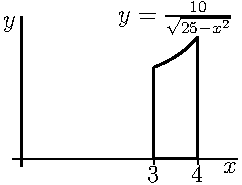
\includegraphics{graphE97D_3}
\end{center}


\noindent(b)
$\displaystyle10\pi\log\frac{9}{4}=20\pi\log\frac{3}{2}$
\qquad (c)
 $20\pi$
\end{answer}

\begin{solution} (a)
Let's graph $y=\dfrac{10}{\sqrt{25-x^2}}$.
We start with the endpoints: $(3,\frac{5}{2})$ and $(4,\frac{10}{3})$. Then we consider the first derivative:
\[\diff{}{x}\left\{\frac{10}{\sqrt{25-x^2}}\right\} = \frac{10x}{\sqrt{25-x^2}^3}\]

Over the interval $[3,4]$, this is always positive, so our function is increasing over the entire interval. The second derivative,

\[\ddiff{2}{}{x}\left\{\frac{10}{\sqrt{25-x^2}}\right\}=\diff{}{x}\left\{\frac{10x}{\sqrt{25-x^2}^3}\right\} = \frac{10(2x^2+25)}{\sqrt{25-x^2}^5},\]

is always positive, so our function is concave up over the entire interval. So,
the region $R$ is:

\begin{center}
       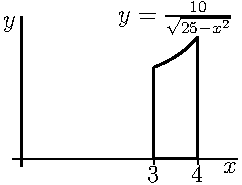
\includegraphics{graphE97D_3}
\end{center}




\noindent (b)
Let $\cV_1$ be the solid obtained by revolving
$R$ about the $x$--axis. The portion of $\cV_1$ with $x$--coordinate
between $x$ and $x+\dee{x}$ is obtained by rotating the red vertical strip in
the figure on the left below about the $x$--axis.
That portion is a disk of radius $\frac{10}{\sqrt{25-x^2}}$ and thickness
$\dee{x}$. The volume of this disk is $\pi\big(\frac{10}{\sqrt{25-x^2}}\big)^2\,\dee{x}$.
So the total volume of $\cV_1$ is
\begin{align*}
\int_3^4\pi{\Big(\frac{10}{\sqrt{25-x^2}}\Big)}^2\ \dee{x}
&=100\pi\int_3^4\frac{1}{25-x^2}\ \dee{x}
=100\pi\int_3^4\frac{1}{(5-x)(5+x)}\ \dee{x} \\
&=10\pi\int_3^4\Big(\frac{1}{5-x}+\frac{1}{5+x}\Big)\ \dee{x}
=10\pi\Big[-\log(5-x)+\log(5+x)\Big]_3^4 \\
&=10\pi\Big[-\log1+\log9+\log2-\log8\Big]
=10\pi\log\frac{9}{4}=20\pi\log\frac{3}{2}
\end{align*}

\begin{center}
       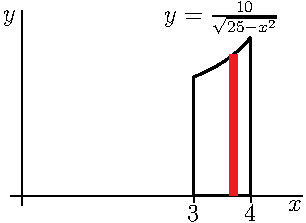
\includegraphics{graphE97D_3l}\qquad\qquad
       \includegraphics{graphE97D_3r}
\end{center}



\noindent (c)
We'll use horizontal washers as in Example  \eref{CLP101}{eg rot yaxis}
of the %\href{http://www.math.ubc.ca/%7Efeldman/m101/clp/clp_notes_101.pdf}{CLP-2 text}.
CLP-2 text.
 \begin{itemize}
\item We cut $\cR$ into thin horizontal  strips of width $\dee{y}$ as in
the figure on the right above.

\item When we rotate $\cR$ about the $y$--axis, each strip sweeps out a thin washer
\begin{itemize}
\item
whose outer radius is $r_{out}=4$, and
\item
whose inner radius is $r_{in}= \sqrt{25-\frac{100}{y^2}}$ when
$y\ge \frac{10}{\sqrt{25-3^2}} = \frac{10}{4}
=\frac{5}{2}$ (see the red strip in the figure on the right above),  and
whose inner radius is $r_{in}= 3$ when $y\le \frac{5}{2}$
(see the blue strip in the figure on the right above) and
\item
whose thickness is $\dee{y}$ and hence
\item
whose volume is
$\pi(r_{out}^2 - r_{in}^2)\dee{y} = \pi\big(\frac{100}{y^2}-9\big)\dee{y}$
when $y\ge \frac{5}{2}$ and  whose volume is
$\pi(r_{out}^2 - r_{in}^2)\dee{y} = 7 \pi\,\dee{y}$
when $y\le \frac{5}{2}$ and

\end{itemize}
\item As our bottommost strip is at $y=0$ and our topmost
strip is at $y=\frac{10}{3}$ (since at the top $x=4$ and $y=  \frac{10}{\sqrt{25-x^2}}
=\frac{10}{\sqrt{25-4^2}} =\frac{10}{3}$), the volume is
\begin{align*}
&\int _{5/2}^{10/3}  \pi\Big(\frac{100}{y^2}-9\Big)\dee{y}
                                                         +\int _ 0^{5/2}7 \pi\,\dee{y} \\
&=\pi{\Big[-\frac{100}{y}-9y\Big]}_{5/2}^{10/3} +\frac{35}{2}\pi\\
&=\pi \Big[-30+40-30+\frac{45}{2}\Big] +\frac{35}{2}\pi\\
&=20\pi
\end{align*}
\end{itemize}

\end{solution}
%%%%%%%%%%%%%%%%%%%



\begin{question}
Find the area of the finite region bounded by the curves $y=\dfrac{4}{3+x^2}$, $y=\dfrac{2}{x(x+1)}$, $x=\dfrac14$, and $x=3$.
\end{question}
\begin{hint}
You'll need to use two regions, because the curves cross.
\end{hint}
\begin{answer}
$\displaystyle2\log\frac53+\frac{4}{\sqrt3}\arctan\frac{1}{4\sqrt3}$
\end{answer}
\begin{solution}
In order to find the area between the curves, we need to know which one is on top, and which on the bottom. Let's start by finding where they meet.
\begin{align*}
\dfrac{4}{3+x^2}&=\frac{2}{x(x+1)}\\
2x^2+2x&=3+x^2\\
x^2+2x-3&=0\\
(x-1)(x+3)&=0
\end{align*}
In the interval $[\frac14,3]$, the curves only meet at $x=1$. So, to find which is on top and on bottom in the intervals $[\frac14,1)$ and $(1,3]$, it suffices to check some point in each interval.
\begin{center}
\begin{tabular}{|c||c|c||c|}
\hline
$x$ & $\frac{4}{3+x^2}$ & $\frac{2}{x(x+1)}$& Top:\\
\hline
$1/2$ &$16/13$ &$8/3$ &$\frac{2}{x(x+1)}$\\
\hline
$2$ &$4/7$ & $1/3$& $\frac{4}{3+x^2}$\\
\hline
\end{tabular}
\end{center}
So, $\frac{2}{x(x+1)}$ is the top function when $\frac{1}{4}\leq x < 1$, and
$\frac{4}{3+x^2}$ is the top function when $1<x \leq 3$. Then the area we want to find is:
\[\mbox{Area}=\int_{\frac14}^1 \left( \frac{2}{x(x+1)} - \frac{4}{3+x^2}\right)~\dee{x}+
\int_{1}^3 \left( \frac{4}{3+x^2} -\frac{2}{x(x+1)}  \right)~\dee{x} \]

We'll need to antidifferentiate both these functions. We can antidifferentiate $\dfrac{2}{x(x+1)}$ using partial fraction decomposition.

\begin{align*}
\frac{2}{x(x+1)}&=\frac{A}{x}+\frac{B}{x+1} = \frac{(A+B)x+A}{x(x+1)}\\
\color{red}A&\color{red}=2,\quad B=-2\\
\int\frac{2}{x(x+1)}~\dee{x}&=\int\left(\frac{2}{x}-\frac{2}{x+1}\right)~\dee{x}=2\log|x|-2\log|x+1|+C\\
&=2\log\left| \frac{x}{x+1}\right|+C
\end{align*}

We can antidifferentiate $\dfrac{4}{3+x^2}$ using the substitution $u=\frac{x}{\sqrt3}$, $\dee{u}=\frac{1}{\sqrt3}~\dee{x}$.
\begin{align*}
\int\frac{4}{3+x^2}~\dee{x}&=
\int\frac{4}{3\left(1+\left(\frac{x}{\sqrt3}\right)^2\right)}~\dee{x}=
\int\frac{4\sqrt3}{3\left(1+u^2\right)}~\dee{u}\\
&=\frac{4}{\sqrt3}\arctan u +C=\frac{4}{\sqrt3}\arctan \left(\frac{x}{\sqrt3}\right) +C
\end{align*}

Now, we can find our area.
\begin{align*}
\mbox{Area}&=\int_{\frac14}^1 \left( \frac{2}{x(x+1)} - \frac{4}{3+x^2}\right)~\dee{x}+
\int_{1}^3 \left( \frac{4}{3+x^2} -\frac{2}{x(x+1)}  \right)~\dee{x}\\
&=\left[2\log\left|\frac{x}{x+1}\right| - \frac{4}{\sqrt3}\arctan\left(\frac{x}{\sqrt3}\right)\right] _{1/4}^1+
\left[ \frac{4}{\sqrt3}\arctan\left(\frac{x}{\sqrt3}\right)-2\log\left|\frac{x}{x+1}\right|\right]_1^3\\
&=\left(2\log\frac{1}{2}- \frac{4}{\sqrt3}\cdot\frac{\pi}{6} - 2\log\frac{1}{5}+\frac{4}{\sqrt3}\arctan\frac{1}{4\sqrt3}\right)+\\
&\hphantom{=} \left(\frac{4}{\sqrt3}\cdot\frac{\pi}{3} - 2\log\frac34 - \frac{4}{\sqrt3}\cdot \frac{\pi}{6}+2\log\frac{1}{2}\right)\\
&=2\log\frac53+\frac{4}{\sqrt3}\arctan\frac{1}{4\sqrt3}
\end{align*}
\end{solution}
%%%%%%%%%%%%%%%%%%%


\begin{Mquestion} Let $F(x) = \displaystyle\int_1^x \frac{1}{t^2-9} \dee{t}$.
\begin{enumerate}[(a)]
\item
Give a formula for $F(x)$ that does not involve an integral.
\item Find $F'(x)$.
\end{enumerate}
\end{Mquestion}
\begin{hint}
For (b), use the Fundamental Theorem of Calculus Part 1.
\end{hint}
\begin{answer}
(a) $\displaystyle\frac{1}{6}\left(\log\left| 2\cdot\frac{x-3}{x+3} \right|\right)$
\qquad
(b) $F'(x) = \frac{1}{x^2-9}$
\end{answer}
\begin{solution}
(a) To antidifferentiate $\dfrac{1}{t^2-9}$, we use a partial fraction decomposition.
\begin{align*}
\frac{1}{t^2-9}&=\frac{1}{(t-3)(t+3)} = \frac{A}{t-3}+\frac{B}{t+3}=\frac{(A+B)t+3(A-B)}{(t-3)(t+3)}\\
A+B&=0,\quad A-B = \frac{1}{3}\\
\color{red}A&\color{red}=\frac{1}{6},\quad B = -\frac{1}{6}\\
F(x)&=\int_1^x\frac{1}{t^2-9}~\dee{x} =
\int_1^x \left(\frac{1/6}{t-3}-\frac{1/6}{t+3}\right)~\dee{x}\\
&=\left[\frac{1}{6}\log|t-3| - \frac{1}{6}\log|t+3|\right]_1^x\\
&=\left(\frac{1}{6}\log|x-3| - \frac{1}{6}\log|x+3|
-\frac{1}{6}\log2 +\frac{1}{6}\log4\right)\\
&=\frac{1}{6}\left(\log\left| 2\cdot\frac{x-3}{x+3} \right|\right)
\end{align*}

(b) Rather than differentiate our answer from (a), we use the Fundamental Theorem of Calculus Part 1 to conclude \[F'(x) = \diff{}{x}\left\{ \displaystyle\int_1^x \frac{1}{t^2-9} \dee{t}\right\} = \frac{1}{x^2-9}\]
\end{solution}


%%%%%%%%%%%%%%%%%%%


%%%%%%%%%%%%%%%%%%%

\section{Numerical Integration}
%
% Copyright 2018 Joel Feldman, Andrew Rechnitzer and Elyse Yeager.
% This work is licensed under a Creative Commons Attribution-NonCommercial-ShareAlike 4.0 International License.
% https://creativecommons.org/licenses/by-nc-sa/4.0/
%
\questionheader{ex:s1.11}

\noindent
Recall that we are using $\log x$ to denote the logarithm of $x$ with
base $e$. In other courses it is often denoted $\ln x$.


%%%%%%%%%%%%%%%%%%
\subsection*{\Conceptual}
%%%%%%%%%%%%%%%%%%
\begin{Mquestion}
Suppose we approximate an object to have volume $1.5 \mathrm{m}^3$, when its exact volume is $1.387 \mathrm{m}^3$. Give the relative error, absolute error, and percent error of our approximation.
\end{Mquestion}
\begin{hint}
The absolute error is  the difference of the two values; the relative error is the absolute error divided by the exact value; the percent error is one hundred times the relative error.
\end{hint}
\begin{answer}
Relative error: $\approx 0.08147$; absolute error: $0.113$; percent error: $\approx 8.147\%$.
\end{answer}
\begin{solution}
The absolute error is the difference between the two values:
\[|1.387-1.5| = 0.113\]
The relative error is the absolute error divided by the exact value:
\[\frac{0.113}{1.387}\approx 0.08147\]
The percent error is 100 times the relative error:
\[\approx 8.147\%\]
\end{solution}
%%%%%%%%%%%%%%%%%%%
\begin{question}
Consider approximating $\displaystyle\int_2^{10} f(x)~\dee{x}$, where $f(x)$ is the function in the graph below.
\begin{center}
\begin{tikzpicture}
\YEaaxis{1.25}{7.25}{1.25}{3.25}
\draw[dotted] (-1,-1) grid[step=0.5] (7,3);
\YExcoord{1}{2}
\YExcoord{5}{10}
\draw[thick, blue] plot[domain=-1:7, samples=50](\x,{.25*\x* sin(\x r)+1.5});
\end{tikzpicture}
\end{center}
\begin{enumerate}[(a)]
\item Draw the rectangles associated with the midpoint rule approximation and $n=4$.
\item Draw the trapezoids associated with the trapezoidal rule approximation and $n=4$.
\end{enumerate}
You don't have to give an approximation.
\end{question}
\begin{hint}
You should have four rectangles in one drawing, and four trapezoids in another.
\end{hint}
\begin{answer}
Midpoint rule:
\begin{center}
\begin{tikzpicture}
\YEaaxis{1.25}{7.25}{1.25}{3.25}
\draw[dotted] (-1,-1) grid[step=0.5] (7,3);
\YExcoord{1}{2}
\YExcoord{5}{10}
\draw[thick, blue] plot[domain=-1:7, samples=50](\x,{.25*\x* sin(\x r)+1.5});
\draw[thick, black, fill=red, fill opacity=0.5] (1,0) rectangle (2,1.87)
(2,0) rectangle (3,1.87)
(3,0) rectangle (4,1.19)
(4,0) rectangle (5,0.4);
\end{tikzpicture}
\end{center}
Trapezoidal rule:
\begin{center}
\begin{tikzpicture}
\YEaaxis{1.25}{7.25}{1.25}{3.25}
\draw[dotted] (-1,-1) grid[step=0.5] (7,3);
\YExcoord{1}{2}
\YExcoord{5}{10}
\draw[thick, blue] plot[domain=-1:7, samples=50](\x,{.25*\x* sin(\x r)+1.5});
\filldraw[thick, black, fill=red, fill opacity=0.5]
(1,0)--(1,1.71)--(2,1.95)|-cycle
(2,0)--(2,1.95)--(3,1.61)|-cycle
(3,0)--(3,1.61)--(4,0.74)|-cycle
(4,0)--(4,0.74)--(5,0.3)|-cycle;
\end{tikzpicture}
\end{center}
\end{answer}
\begin{solution}
Midpoint rule:
\begin{center}
\begin{tikzpicture}
\YEaaxis{1.25}{7.25}{1.25}{3.25}
\draw[dotted] (-1,-1) grid[step=0.5] (7,3);
\YExcoord{1}{2}
\YExcoord{5}{10}
\draw[thick, blue] plot[domain=-1:7, samples=50](\x,{.25*\x* sin(\x r)+1.5});
\draw[thick, black, fill=red, fill opacity=0.5] (1,0) rectangle (2,1.87)
(2,0) rectangle (3,1.87)
(3,0) rectangle (4,1.19)
(4,0) rectangle (5,0.4);
\end{tikzpicture}
\end{center}
Trapezoidal rule:
\begin{center}
\begin{tikzpicture}
\YEaaxis{1.25}{7.25}{1.25}{3.25}
\draw[dotted] (-1,-1) grid[step=0.5] (7,3);
\YExcoord{1}{2}
\YExcoord{5}{10}
\draw[thick, blue] plot[domain=-1:7, samples=50](\x,{.25*\x* sin(\x r)+1.5});
\filldraw[thick, black, fill=red, fill opacity=0.5]
(1,0)--(1,1.71)--(2,1.95)|-cycle
(2,0)--(2,1.95)--(3,1.61)|-cycle
(3,0)--(3,1.61)--(4,0.74)|-cycle
(4,0)--(4,0.74)--(5,0.3)|-cycle;
\end{tikzpicture}
\end{center}
\end{solution}
%%%%%%%%%%%%%%%%%%%
\begin{Mquestion}
Let $f(x) = -\dfrac{1}{12}x^4+\dfrac{7}{6}x^3-3x^2$.
\begin{enumerate}[(a)]
\item Find a reasonable value $M$ such that $|f''(x)| \leq M$ for all $1 \leq x \leq 6$.
\item Find a reasonable value $L$ such that $|f^{(4)}(x)| \leq L$ for all $1 \leq x \leq 6$.
\end{enumerate}
\end{Mquestion}
\begin{hint}
Sketch the second derivative--it's quadratic.
\end{hint}
\begin{answer} $M=6.25$, $L=2$
\end{answer}
\begin{solution}
\begin{enumerate}[(a)]
\item
Differentiating, we find $f''(x) = -x^2+7x-6$. Since $f''(x)$ is quadratic, we have a pretty good idea of what it looks like.
\begin{itemize}
\item It factors as $f(x)  = -(x-6)(x-1)$, so its two roots are at $x=6$ and $x=1$.
\item The ``flat part" of the parabola is at $x=3.5$ (since this is exactly half way  between $x=1$ and $x=6$; alternately, we can check that $f'''(3.5)=0$).
\item
 Since the coefficient of $x^2$ is negative, $f(x)$ is increasing from $-\infty$ to $3.5$, then decreasing from $3.5$ to $\infty$.
 \end{itemize}
 Therefore, over the interval $[1,6]$, the largest positive value of $f''(x)$ occurs when $x=3.5$, and this is $f''(3.5) = -(3.5-6)(3.5-1)=6.25$.
\begin{center}
\begin{tikzpicture}
\YEaaxis{.5}{3.5}{2.5}{2.5}
\draw[thick, blue] plot[domain=0:7, samples=50](\x/2,{(-\x*\x+7*\x-6)/3}) node[above right]{$y=f''(x)$};
\YExcoord{.5}{1}
\YExcoord{3}{6}
\YEycoord{2.125}{6.25}
\end{tikzpicture}
\end{center}
So, we take $M=6.25$.

\item We differentiate further to find $f^{(4)}(x)=-2$. This is constant everywhere, so we take $L=|-2|=2$.
\end{enumerate}
\end{solution}
%%%%%%%%%%%%%%%%%%%
\begin{question}\label{prob_s1.11_approxM}
Let $f(x) = x\sin x+2\cos x$.
 Find a reasonable value $M$ such that $|f''(x)| \leq M$ for all $-3 \leq x \leq 2$.
\end{question}
\begin{hint}
You don't have to find the actual, exact maximum the second derivative achieves--you only have to give a reasonable ``ceiling" that it never breaks through.
\end{hint}
\begin{answer}
One reasonable answer is $M=3$.
\end{answer}
\begin{solution}
Let's start by differentiating.
\begin{align*}
f(x)&=x\sin x +2\cos x\\
f'(x)&=x\cos x + \sin x - 2\sin x =x\cos x - \sin x\\
f''(x)&=-x\sin x + \cos x -\cos x = -x\sin x
\end{align*}
For any value of $x$, $|\sin x| \leq 1$. When $-3 \leq x \leq 2$, then $|x| \leq 3$. So, it is true (and not unreasonably sloppy) that
\[f''(x) \leq 3\]
whenever $x$ is in the interval $[-3,2]$. So, we can take $M=3$.

Note that $|f''(x)|$ is actually \emph{smaller} than 3 whenever $x$ is in the interval $[-3,2]$, because when $x=-3$, $\sin x \neq 1$. In fact, since 3 is pretty close to $\pi$, $\sin 3$ is pretty small. (The actual maximum value of $|f''(x)|$ when $-3\leq x\leq 2$ is about 1.8.) However, we find  parameters like $M$ for the purpose of computing error bounds. There is often not much to be gained from taking the time to find the actual maximum of a function, so we content ourselves with reasonable upper bounds.
Question~\ref{prob_s1.11_exactM} has a further investigation of ``sloppy" bounds like this.
\end{solution}
%%%%%%%%%%%%%%%%%%%


\begin{Mquestion}\label{prob_s1.11:approxerror1}
Consider the quantity $A=\displaystyle\int_{-\pi}^{\pi} \cos x~\dee{x}$.
\begin{enumerate}[(a)]
\item Find the upper bound on the error using Simpson's rule with $n=4$ to approximate $A$ using Theorem~\eref{CLP101}{thm num int err} in the CLP--II text.
\item Find the Simpson's rule approximation of $A$ using $n=4$.
\item What is the (actual) absolute error in the Simpson's rule approximation of $A$ with $n=4$?
\end{enumerate}
\end{Mquestion}
\begin{hint}
To compute the upper bound on the error, find an upper bound on the fourth derivative of cosine, then use Theorem~\eref{CLP101}{thm num int err} in the CLP--II text.

To find the actual error, you need to find the actual value of $A$.
\end{hint}
\begin{answer}
(a) $\dfrac{\pi^5}{180\cdot8}$
\qquad (b) $0$ \qquad (c) $0$
\end{answer}
\begin{solution}
\begin{enumerate}[(a)]
\item Let $f(x) = \cos x$. Then $f^{(4)}(x)=\cos x$, so $|f^{(4)}(x)| \leq 1$ when $-\pi \leq x \leq \pi$. So, using $L=1$, we find the upper bound of the error using Simpson's rule with $n=4$ is:
\[\frac{L(b-a)^5}{180 n^4} = \frac{(2\pi)^5}{180\cdot 4^4} = \frac{\pi^5}{180\cdot8}\approx 0.2\]
The error bound comes from Theorem~\eref{CLP101}{thm num int err} in the CLP--II text.
We used a calculator to find the approximate decimal value.
\item
We use the general form of Simpson's rule (Equation~\eref{CLP101}{eq:SIMPrule} in
the CLP--II text) with $\Delta x = \frac{b-a}{n}=\frac{2\pi}{4} = \frac{\pi}{2}$.
\begin{align*}
A& \approx \frac{\Delta x}{3}\left(f(x_0) + 4f(x_1)+2f(x_2)+4f(x_3)+f(x_4)\right)
\\&=\frac{\pi/2}{3}\left(f(-\pi) + 4f(\tfrac{-\pi}{2})+2f(0)+4f(\tfrac{\pi}{2})+f(\pi)\right)\\
&= \frac{\pi}{6}\left(-1 + 4(0)+2(1)+4(0)-1\right)=0
\end{align*}
\item
To find the actual error in our approximation, we compare the approximation from (b) to the exact value of $A$. In fact, $A=0$: this is a fact you've probably seen before by considering the symmetry of cosine, but it's easy enough to calculate:
\[A = \int_{-\pi}^{\pi} \cos x~\dee{x}= \sin \pi - \sin (-\pi) = 0\]
So, our approximation was exactly the same as our exact value. The absolute error is 0.
\end{enumerate}
Remark: the purpose of this question was to remind you that the error bounds we calculate are not (usually) the same as the actual error. Often our approximations are better than we give them credit for. In normal circumstances, we would be approximating an integral precisely to avoid evaluating it exactly, so we wouldn't find our exact error. The bound is a quick way of ensuring that our approximation is not \emph{too} far off.
\end{solution}
%%%%%%%%%%%%%%%%%%%

\begin{question}
Give a function $f(x)$ such that:
\begin{itemize}
\item $f''(x) \leq 3$ for every $x$ in $[0,1]$, and
\item  the error using the trapezoidal rule approximating $\displaystyle\int_0^1 f(x)~\dee{x}$ with $n=2$ intervals is exactly $\dfrac{1}{16}$.
\end{itemize}
\end{question}
\begin{hint}
Find a function with $f''(x)=3$ for all $x$ in $[0,1]$.
\end{hint}
\begin{answer}
Possible answers: $f(x) = \dfrac{3}{2}x^2+Cx+D$ for any constants $C$, $D$.
\end{answer}
\begin{solution}
Using Theorem~\eref{CLP101}{thm num int err} in the CLP--II text, the error using the trapezoidal rule as described is \emph{at most}
\[\dfrac{M(b-a)^3}{12\cdot n^2} = \dfrac{M}{48} \leq \frac{3}{48}=\frac{1}{16}.\] So, we're really being asked to find a function with the maximum possible error using the trapezoidal rule, given its second derivative.

With that in mind, our function should have the largest second derivative possible: let's set $f''(x)=3$ for every $x$. Then:
\begin{align*}
&&f''(x)&=3\\
&&f'(x)&=3x+C\\
&&f(x)&=\frac{3}{2}x^2+Cx+D
\intertext{for some constants $C$ and $D$. Now we can find the exact and approximate values of $\displaystyle\int_0^1 f(x)~\dee{x}$.}
&\mbox{Exact:}&\int_0^1 f(x)~\dee{x}&=\int_0^1 \left(\frac{3}{2}x^2+Cx+D\right)~\dee{x}\\
&&&=\left[\frac{1}{2}x^3+\frac{C}{2}x^2+Dx\right]_0^1\\
&&&=\textcolor{blue}{\frac{1}{2}+\frac{C}{2}+D}\\
&\mbox{Approximate:}&\int_0^1 f(x)~\dee{x}&\approx \Delta x \left[\frac{1}{2}f(0)+f(\tfrac{1}{2})+\frac{1}{2}f(1)\right]\\
&&&=\frac{1}{2}\left[\frac{1}{2}(D)+\left(\frac{3}{8}+\frac{C}{2}+D\right)+\frac{1}{2}\left(\frac{3}{2}+C+D\right)\right]\\
&&&=\frac{1}{2}\left[\frac{9}{8}+C+2D\right]\\
&&&=\textcolor{red}{\frac{9}{16}+\frac{C}{2}+D}
\end{align*}
So, the absolute error associated with the trapezoidal approximation is:
\[\left|\left(\textcolor{blue}{\frac{1}{2}+\frac{C}{2}+D}\right)  - \left(\textcolor{red}{\frac{9}{16}+\frac{C}{2}+D}\right) \right| = \frac{1}{16}\]
So, for any constants $C$ and $D$, $f(x) = \frac{3}{2}x^2+Cx+D$ has the desired error.

Remark: contrast this question with Question~\ref{prob_s1.11:approxerror1}. In this problem, our absolute error was exactly as bad as the bound predicted, but sometimes it is much  better. The thing to remember is that, in general, we \emph{don't know} our  absolute error. We only guarantee that it's not any worse than some worst-case-scenario bound.
\end{solution}
%%%%%%%%%%%%%%%%%%%

\begin{question}\label{prob_s1.11:mom}
Suppose my mother is under 100 years old, and I am under 200 years old.\footnote{We're going somewhere with this.} Who is older?
\end{question}
\begin{hint}
You're allowed to use common sense for this one.
\end{hint}
\begin{answer}
my mother
\end{answer}
\begin{solution}
Under any reasonable assumptions\footnote{Anyone caught trying to come up with a scenario in which I am older than my mother will be sent to maximum security grad school.}, my mother is older than I am.
\end{solution}
%%%%%%%%%%%%%%%%%%%


\begin{question}
\begin{enumerate}[(a)]
\item True or False: for fixed positive constants $M$, $n$, $a$, and $b$, with $b>a$,\[\dfrac{M}{24}\dfrac{(b-a)^3}{n^2}\leq \dfrac{M}{12}\dfrac{(b-a)^3}{n^2}\]
\item True or False: for a function $f(x)$ and fixed constants $n$, $a$, and $b$, with $b>a$, the $n$-interval midpoint approximation of $\displaystyle\int_a^b f(x)~\dee{x}$ is more accurate than the $n$-interval trapezoidal approximation.
\end{enumerate}
\end{question}
\begin{hint}
For part (b), consider Question~\ref{prob_s1.11:mom}.
\end{hint}
\begin{answer}
(a) true \qquad (b) false
\end{answer}
\begin{solution}
\noindent (a) Since both expressions are positive, and $\frac{1}{24} \leq \frac{1}{12}$, the inequality is true.\\

\noindent (b) False. The reasoning is the same as in Question~\ref{prob_s1.11:mom}. The \emph{error bound} given by Theorem 1.11.12 is always better for the trapezoid rule, but this doesn't necessarily mean the \emph{error} is better.

To see how the trapezoid approximation could be better than the corresponding midpoint approximation in some cases, consider the function $f(x)$ sketched below.
\begin{center}
\begin{tikzpicture}
\YEaaxis{1}{4}{1}{3}
\YExcoord{1}{a}
\YExcoord{2}{}
\YExcoord{3}{b}
\draw[thick, blue, rounded corners] (0,.1)--(1.9,.3)--(1.95,3) arc(180:360:.4mm)-- (2.1,.3)--(4,.1);
\end{tikzpicture}
\end{center}

The trapezoidal approximation of $\displaystyle\int_a^b f(x)~\dee{x}$ with $n=1$ misses the thin spike, and gives a mild underapproximation. By contrast, the midpoint approximation with $n=1$ takes the spike as the height of the entire region, giving a vast overapproximation.

\begin{center}
\begin{tikzpicture}
\draw[thick, red, fill=red, fill opacity=0.2] (1,.2) rectangle (3,0);

\YEaaxis{1}{4}{1}{3}
\YExcoord{1}{a}
\YExcoord{2}{}
\YExcoord{3}{b}
\draw[thick, blue, rounded corners] (0,.1)--(1.9,.3)--(1.95,3) arc(180:360:.4mm)-- (2.1,.3)--(4,.1);
\draw[red] (1,.2) node[vertex]{};
\draw[red] (3,.2) node[vertex]{};
\draw (2,-1) node {trapezoidal};
\end{tikzpicture}
\hspace{2cm}
\begin{tikzpicture}
\draw[red, thick, fill=red, fill opacity=0.2] (1,3) rectangle (3,0);

\YEaaxis{1}{4}{1}{3}
\YExcoord{1}{a}
\YExcoord{2}{}
\YExcoord{3}{b}
\draw[thick, blue, rounded corners] (0,.1)--(1.9,.3)--(1.95,3) arc(180:360:.4mm)-- (2.1,.3)--(4,.1);
\draw[red] (2,3) node[vertex]{};
\draw (2,-1) node {midpoint};
\end{tikzpicture}
\end{center}

\end{solution}
%%%%%%%%%%%%%%%%%%%



\begin{Mquestion}[2015A]
Decide whether the following statement is true or false.
If false, provide a counterexample. If true, provide a brief justification.

\begin{quote}\color{blue}
When $f(x)$ is positive and concave up, any trapezoidal rule approximation for $\displaystyle\int_{a}^{b} f(x) \,\dee{x}$ will be an upper estimate for $\displaystyle\int_{a}^{b} f(x) \,\dee{x}$.
\end{quote}
\end{Mquestion}

\begin{hint}
Draw a sketch.
\end{hint}

\begin{answer}
True. Because $f(x)$ is positive and concave up,
the graph of $f(x)$ is always below the top edges of the trapezoids
used in the trapezoidal rule.

\begin{center}
\begin{tikzpicture}
\YEaaxis{3}{3}{1}{3}
\draw[thick, blue] plot[domain=-3:3](\x,{\x*\x/4+.5}) node[right]{$y=f(x)$};
\draw[red] (-1,.75) node[vertex](a){};
\draw[red] (2,1.5) node[vertex](b){};
\filldraw[red, thick, fill opacity=0.1] (-1,.75)|-(2,0)--(2,1.5)--(-1,.75);
\end{tikzpicture}
\end{center}
\end{answer}

\begin{solution}
True. Because $f(x)$ is positive and concave up,
the graph of $f(x)$ is always below the top edges of the trapezoids
used in the trapezoidal rule.

\begin{center}
\begin{tikzpicture}
\YEaaxis{3}{3}{1}{3}
\draw[thick, blue] plot[domain=-3:3](\x,{\x*\x/4+.5}) node[right]{$y=f(x)$};
\draw[red] (-1,.75) node[vertex](a){};
\draw[red] (2,1.5) node[vertex](b){};
\filldraw[red, thick, fill opacity=0.1] (-1,.75)|-(2,0)--(2,1.5)--(-1,.75);
\end{tikzpicture}
\end{center}
\end{solution}
%%%%%%%%%%%%%%%%%%%

\begin{question}
Give a polynomial $f(x)$ with the property that
 the Simpson's rule approximation of $\displaystyle\int_a^b f(x)~\dee{x}$ is exact for all $a$, $b$, and $n$.
\end{question}
\begin{hint}
The error bound for the approximation is given in Theorem~\eref{CLP101}{thm num int err} in the CLP--II text. You want this bound to be zero.
\end{hint}
\begin{answer}
Any polynomial of degree at most 3 will do. For example, $f(x)=5x^3-27$, or $f(x)=x^2$.
\end{answer}
\begin{solution}
According to Theorem~\eref{CLP101}{thm num int err}  in the CLP--II text, the error associated with the Simpson's rule approximation is no more than $\dfrac{L}{180}\dfrac{(b-a)^5}{n^4}$, where $L$ is a constant such that $|f^{(4)}(x)| \leq L$ for all $x$ in $[a,b]$. If $L=0$, then the error is no more than 0 regardless of $a$, $b$, or $n$--that is, the approximation is exact.

Any polynomial $f(x)$ of degree at most 3 has $f^{(4)}(x)=0$ for all $x$. So, any polynomial of degree at most 3 is an acceptable answer. For example, $f(x)=5x^3-27$, or $f(x)=x^2$.
\end{solution}
%%%%%%%%%%%%%%%%%%%



%%%%%%%%%%%%%%%%%%
\subsection*{\Procedural}
%%%%%%%%%%%%%%%%%%
\Instructions{Questions
\ref{prob_s1.11_int1} and \ref{prob_s1.11_int2}
ask you to approximate a given integral  using the formulas in Equations~\eref{CLP101}{eq:MPrule},
\eref{CLP101}{eq:TRPrule}, and \eref{CLP101}{eq:SIMPrule} in the CLP--II text.}
\begin{Mquestion}\label{prob_s1.11_int1}
Write out all three approximations of $\displaystyle\int_0^{30} \frac{1}{x^3+1}~\dee{x}$ with $n=6$. (That is: midpoint, trapezoidal, and Simpson's.) You do not need to simplify your answers.
\end{Mquestion}
\begin{hint}
Follow the formulas in Equations~\eref{CLP101}{eq:MPrule},
\eref{CLP101}{eq:TRPrule}, and \eref{CLP101}{eq:SIMPrule} in the CLP--II text.
\end{hint}
\begin{answer}

Midpoint:\\[10pt]
$\displaystyle
\int_0^{30} \frac{1}{x^3+1}\,\dee{x}\approx\left[\tfrac{1}{\left(2.5\right)^3+1}
+\tfrac{1}{\left(7.5\right)^3+1}
+\tfrac{1}{\left(12.5\right)^3+1}
+\tfrac{1}{\left(17.5\right)^3+1}
+\tfrac{1}{\left(22.5\right)^3+1}
+\tfrac{1}{\left(27.5\right)^3+1}
\right]5
$

Trapezoidal:\\[10pt]
$\displaystyle\int_0^{30} \frac{1}{x^3+1}\,\dee{x}
\approx\left[
\frac{1/2}{0^3+1}+
\frac{1}{5^3+1}+
\frac{1}{10^3+1}+
\frac{1}{15^3+1}+
\frac{1}{20^3+1}+
\frac{1}{25^3+1}+
\frac{1/2}{30^3+1}
\right]5$

Simpson's:\\[10pt]
$
\displaystyle\int_0^{30} \frac{1}{x^3+1}\,\dee{x}\approx
\Big[\frac{1}{{0}^3+1}\!+\frac{4}{{5}^3+1}\!+\frac{2}{{10}^3+1}\!+\frac{4}{{15}^3+1}\!+\frac{2}{{20}^3+1}\!+\frac{4}{{25}^3+1}\!+ \frac{1}{{30}^3+1}\Big]\frac{5}{3}
$
\end{answer}
\begin{solution}
\begin{itemize}
\item For all three approximations, $\Delta x = \dfrac{b-a}{n}=\dfrac{30-0}{6}=5$.


\item For the trapezoidal rule and Simpson's rule, the $x$-values where we evaluate $\dfrac{1}{x^3+1}$ start at $x=a=0$ and move up by $\Delta x = 5$:  $x_0=0$, $x_1=5$,
 $x_2=10$, $x_3=15$,
  $x_4=20$, $x_5=25$, and $x_6=30$.

  \begin{center}
  \begin{tikzpicture}[scale=1.8]
  \draw[<->, thick] (-1,0)--(7,0);
  \foreach \x in {0,...,6}{
  	\MULTIPLY{\x}{5}{\l}
	\YExcoord{\x}{\atp{\l}{x_{\x}}}}
  \end{tikzpicture}
  \end{center}

\item For the midpoint rule, the $x$-values where we evaluate $\dfrac{1}{x^3+1}$ start at $x=2.5 = \frac{x_0+x_1}{2}$ and move up by $\Delta x = 5$:  $\bar x_1=2.5$, $\bar x_2=7.5$,
 $\bar x_3=12.5$, $\bar x_4=17.5$,
  $\bar x_5=22.5$, and $\bar x_6=27.5$.


  \begin{center}
  \begin{tikzpicture}[scale=1.8]
  \draw[<->, thick] (-1,0)--(7,0);
  \foreach \x in {0,...,6}{
  	\MULTIPLY{\x}{5}{\l}
	\color{gray}
	\YExcoord{\x}{\atp{\l}{x_{\x}}}
	\ADD{\x}{.5}{\y};
	\ADD{\l}{2.5}{\m}}
  \foreach \x in {1,...,6}{
  	\MULTIPLY{\x}{5}{\l}
	\SUBTRACT{\x}{.5}{\y};
	\SUBTRACT{\l}{2.5}{\m}
	\color{red}
	\YExcoord{\y}{\atp{\m}{\bar x_{\x}}}}

  \end{tikzpicture}
  \end{center}

\item  Following Equation~\eref{CLP101}{eq:MPrule} in the CLP--II text,
the midpoint rule approximation is:
\begin{align*}
\int_0^{30} \frac{1}{x^3+1}\,\dee{x}&\approx\Big[f(\bar x_1)+f(\bar x_2)+\cdots
+f(\bar x_n)\Big]\De x\\
&=\left[\tfrac{1}{\left(2.5\right)^3+1}
+\tfrac{1}{\left(7.5\right)^3+1}
+\tfrac{1}{\left(12.5\right)^3+1}
+\tfrac{1}{\left(17.5\right)^3+1}
+\tfrac{1}{\left(22.5\right)^3+1}
+\tfrac{1}{\left(27.5\right)^3+1}
\right]5
\end{align*}

 \item
  Following Equation~\eref{CLP101}{eq:TRPrule} in the CLP--II text, the trapezoidal rule approximation is:
\begin{align*}
\int_0^{30} \frac{1}{x^3+1}\,\dee{x}
&\approx\Big[\half f(x_0)+f(x_1)+f(x_2)+\cdots+ f(x_{n-1})+\half f(x_n)\Big]\De x\\
&=\left[
\frac{1/2}{0^3+1}+
\frac{1}{5^3+1}+
\frac{1}{10^3+1}+
\frac{1}{15^3+1}+
\frac{1}{20^3+1}+
\frac{1}{25^3+1}+
\frac{1/2}{30^3+1}
\right]5
\end{align*}

\item Following Equation~\eref{CLP101}{eq:SIMPrule} in the CLP--II text, the Simpson's rule approximation is:
\begin{align*}
\int_0^{30} \frac{1}{x^3+1}\,\dee{x}
&\approx\Big[f(x_0)\!+4f(x_1)\!+2f(x_2)\!+4f(x_3)\!+2f(x_4)\!+4f(x_{5})\!+ f(x_6)\Big]\tfrac{\De x}{3}\\
&=\Big[\frac{1}{{0}^3+1}\!+\frac{4}{{5}^3+1}\!+\frac{2}{{10}^3+1}\!+\frac{4}{{15}^3+1}\!+\frac{2}{{20}^3+1}\!+\frac{4}{{25}^3+1}\!+ \frac{1}{{30}^3+1}\Big]\frac{5}{3}
\end{align*}

\end{itemize}
\end{solution}
%%%%%%%%%%%%%%%%%%%


\begin{question}[M121 2012A]\label{prob_s1.11_int2}
Find the midpoint rule approximation to $\displaystyle\int_0^\pi \sin x\ \dee{x}$
with $n = 3$.
\end{question}

\begin{hint}
See Section~\eref{CLP101}{sec:midpointRule} in the
%\href{http://www.math.ubc.ca/%7Efeldman/m101/clp/clp_notes_101.pdf}{CLP--II text}.
CLP--II text. You should be able to simplify your answer to an exact value (in terms of $\pi$).
\end{hint}

\begin{answer}
$\dfrac{2\pi}{3}$
\end{answer}

\begin{solution}
By Equation~\eref{CLP101}{eq:MPrule} in the CLP--II text,
the midpoint rule approximation
to $\int_a^b f(x)\ \dee{x}$ with $n=3$ is
\begin{align*}
\int_a^b f(x)\,\dee{x}\approx\big[f(\bar x_1)+f(\bar x_2)+f(\bar x_3)\big]\De x
\end{align*}
where $\De x = \tfrac{b-a}{3}$ and
\begin{alignat*}{7}
x_0&=a&\quad
x_1&=a+\De x&\quad
x_2&=a+2\De x&\quad
x_3&=b\\
& &
\bar x_1&=\tfrac{x_0+x_1}{2}&
\bar x_2&=\tfrac{x_1+x_2}{2}&
\bar x_3&=\tfrac{x_2+x_3}{2}
\end{alignat*}
For this problem, $a=0$, $b=\pi$ and $f(x) = \sin x$, so that
$\De x = \tfrac{\pi}{3}$  and
\begin{alignat*}{7}
x_0&=0&\quad
x_1&=\tfrac{\pi}{3}&\quad
x_2&=\tfrac{2\pi}{3}&\quad
x_3&=\pi\\
& &
\bar x_1&=\tfrac{\pi}{6}&
\bar x_2&=\tfrac{\pi}{2}&
\bar x_3&=\tfrac{5\pi}{6}
\end{alignat*}



  \begin{center}
  \begin{tikzpicture}[scale=1.8]
  \draw[<->, thick] (-1,0)--(7,0);
	\YExcoord{0}{\atp{0}{x_{0}}}
	\YExcoord{6}{\atp{\pi}{x_{3}}}
	\YExcoord{2}{\atp{\pi/3}{x_{1}}}
	\YExcoord{4}{\atp{2\pi/3}{x_{2}}}
\color{red}
	\YExcoord{1}{\atp{\pi/6}{\bar x_{1}}}
	\YExcoord{3}{\atp{\pi/2}{\bar x_{2}}}
	\YExcoord{5}{\atp{5\pi/6}{\bar x_{3}}}
  \end{tikzpicture}
  \end{center}


Therefore,
\begin{align*}
\int_0^\pi \sin x\ \dee{x}
&\approx\left[\sin\frac{\pi}{6}
            +\sin \frac{\pi}{2}
            +\sin \frac{5\pi}{6}\right]\frac{\pi}{3}
=\left[\frac{1}{2}
            +1
            +\frac{1}{2}\right]\frac{\pi}{3}
=\frac{2\pi}{3}
\end{align*}

\end{solution}
%%%%%%%%%%%%%%%%%%%
\Instructions{Questions~\ref{prob_s1.11_tableproblem1} though
\ref{prob_s1.11_tableproblem3}
ask you to approximate a quantity based on observed data.}
%%%%%%%%%%%%%%%%%%%


\begin{question}[1997D]\label{prob_s1.11_tableproblem1}
The solid $V$ is 40 cm high and the horizontal cross sections
are circular disks. The table below gives the diameters of the cross sections
in centimeters at 10 cm intervals. Use the trapezoidal rule to estimate
the volume of $V$.

\renewcommand{\arraystretch}{1.1}
\begin{center}
     \begin{tabular}{|l|c|c|c|c|c|}
          \hline
          height&0&10&20&30&40  \\
          \hline
          diameter&24&16&10&6&4 \\
          \hline
     \end{tabular}
\end{center}
\renewcommand{\arraystretch}{1.0}
\end{question}

\begin{hint}
See Section~\eref{CLP101}{sec:trapRule} in the
%\href{http://www.math.ubc.ca/%7Efeldman/m101/clp/clp_notes_101.pdf}{CLP--II text}.
CLP--II text.
To set up the volume integral, see Example \eref{CLP101}{eg:VOLb} in the
%\href{http://www.math.ubc.ca/%7Efeldman/m101/clp/clp_notes_101.pdf}{CLP--II text}.
CLP--II text. Note the dimensions given for the cross sections are diameters, not radii.
\end{hint}

\begin{answer}
$1720\pi\approx 5403.5\ {\rm cm}^3$
\end{answer}

\begin{solution}
Let $f(x)$ denote the diameter at height $x$.
As in Example \eref{CLP101}{eg:VOLb} of the
%\href{http://www.math.ubc.ca/%7Efeldman/m101/clp/clp_notes_101.pdf}{CLP--II text}.
CLP--II text, we slice $V$  into thin horizontal ``pancakes'', which in
this case are circular.

\begin{center}
\begin{tikzpicture}
\draw plot[domain=0:4]({(\x*\x+\x+4)/6} ,4-\x);
\draw plot[domain=0:4]({1-(\x*\x+\x+4)/6} ,4-\x);
\draw (.6667,4) arc(0:360:1.667mm and 0.666 mm);
\draw (-3,0) arc (180:360:35mm and 7mm);
\draw[dashed] (-2.95,0) arc (170:10:35mm and 7mm);
%\draw (-1,0) grid[] (4,4);
\draw (.5,3) node[shape=ellipse, minimum width=1cm, minimum height=2mm, fill, fill opacity=0.2, draw]{};
\filldraw[fill opacity=0.3] (0,3)--(0,2.8) arc (180:360: .5cm and 2mm)--(1,3) arc (0:-180: .5cm and 2mm);
\draw (-1,2.95) node[left]{$\dee{x}$};
\draw (-.7,2.8)-|(-.9,3.0) --(-.7,3.0);
\draw[|-|] (0,2.25)--(1,2.25) node[midway, below]{$f(x)$};
\draw[help lines, <->] (-4,-.5)--(-4,4.5) node[above]{$x$};
\end{tikzpicture}
\end{center}

\begin{itemize}
\item We are told that the pancake at height $x$ is a circular disk
of diameter $f(x)$ and so
\item has cross-sectional area $\pi\big(\frac{f(x)}{2}\big)^2$ and
thickness $\dee{x}$ and hence
\item has volume $\pi\big(\frac{f(x)}{2}\big)^2\dee{x}$.
\end{itemize}


\noindent Hence the volume of $V$ is
\begin{align*}
\int_0^{40}\pi\Big{[\frac{f(x)}{2}\Big]}^2\,\dee{x}
&\approx \frac{\pi}{4}10\Big[\half f(0)^2+f(10)^2+f(20)^2+f(30)^2+\half
f(40)^2\Big]\\
&=\frac{\pi}{4}10\Big[\half 24^2+16^2+10^2+6^2+\half 4^2\Big]\\
&=688\times 2.5\pi
=1720\pi\approx 5403.5
\end{align*}
where we have approximated the integral using the trapezoidal rule with $\De
x=10$, and used a calculator to get a decimal approximation.


\end{solution}
%%%%%%%%%%%%%%%%%%%
\begin{question}[1996D]\label{prob_s1.11tableproblem2}
A $6$ metre long cedar log has cross sections that are approximately
circular. The diameters of the log, measured at one metre intervals, are
given below:

\renewcommand{\arraystretch}{1.1}
\begin{center}
     \begin{tabular}{|l|c|c|c|c|c|c|c|}
          \hline
          metres from left end of log&0&1&2&3&4&5&6  \\
          \hline
          diameter in metres         &1.2&1&0.8&0.8&1&1&1.2 \\
          \hline
     \end{tabular}
\end{center}
\renewcommand{\arraystretch}{1.0}

\noindent Use Simpson's Rule to estimate the volume of the log.

\end{question}

\begin{hint}
See Section \eref{CLP101}{sec:Simpson} in the
%\href{http://www.math.ubc.ca/%7Efeldman/m101/clp/clp_notes_101.pdf}{CLP--II text}.
CLP--II text, and compare to Question~\ref{prob_s1.11_tableproblem1}. Note the table gives diameters, not radii.
\end{hint}

\begin{answer}
$\displaystyle\frac{\pi}{12}(16.72)\approx4.377\ {\rm m}^3$
\end{answer}

\begin{solution}
 Let $f(x)$ be the diameter a distance $x$ from the left end of
the log.
If we slice our log into thin disks, the disks $x$ metres from the left end of the log has
\begin{itemize}
\item radius $\frac{f(x)}{2}$,
\item width $\dee{x}$, and so
\item volume $\pi\left(\frac{f(x)}{2}\right)^2~\dee{x}=\frac{\pi}{4}f(x)^2~\dee{x}$.
\end{itemize}

\begin{center}
\begin{tikzpicture}
\draw plot[domain=0:3.14]({3*\x},{-sin(\x r)/3});
\draw plot[domain=0:3.14]({3*\x},{-2+sin(\x r)/3});
\draw(0,-2) arc(270:90: 2.5mm and 1cm);
\draw[dashed](0,-2) arc(270:-270: 2.5mm and 1cm);
\draw (9.42,-1) node[shape=ellipse, minimum height=2cm, minimum width=5mm, draw]{};
\draw[] (4.71,-1) node[shape=ellipse, minimum height=1.33cm, minimum width=4mm, draw, fill, fill opacity=0.1]{};
\filldraw[fill opacity=0.3] (4.71,-.33) -- (4.51,-.33 )arc (90:270:2mm and 6.67mm) --(4.71,-1.67)
arc (270:90:2mm and 6.67mm) ;
\draw[<->, help lines] (-1,-3)--(11,-3) node[right]{$x$};
\draw[|-|] (3.5,-.4)--(3.5,-1.6) node[midway, left]{$f(x)$};
\draw[|-|] (4.5,0)--(4.7,0) node[above, midway]{$\dee{x}$};
\end{tikzpicture}
\end{center}

Using Simpson's Rule with $\De
x=1$,
the volume
of the log is:
\begin{align*}
V=\int_0^6 \frac{\pi}{4}f(x)^2\,\dee{x}
&\approx\frac{\pi}{4}\frac{1}{3}
\Big[f(0)^2+4f(1)^2+2f(2)^2+4f(3)^2+2f(4)^2+4f(5)^2+f(6)^2\Big]\\
&=\frac{\pi}{12}
\Big[1.2^2+4(1)^2+2(0.8)^2+4(0.8)^2+2(1)^2+4(1)^2+1.2^2\Big]\\
&=\frac{\pi}{12}(16.72)\\
&\approx4.377\ {\rm m}^3
\end{align*}
where we used a calculator to approximate the decimal value.
\end{solution}
%%%%%%%%%%%%%%%%%%%

\begin{question}[1998A]
 The circumference of an 8 metre high tree at different heights
above the ground is given in the table below. Assume that all horizontal
cross--sections of the tree are circular disks.

\renewcommand{\arraystretch}{1.1}
\begin{center}
     \begin{tabular}{|l|c|c|c|c|c|}
          \hline
          height (metres) &0&2&4&6&8  \\
          \hline
          circumference (metres) &1.2&1.1&1.3&0.9&0.2\\
          \hline
     \end{tabular}
\end{center}
\renewcommand{\arraystretch}{1.0}

\noindent Use Simpson's rule to approximate the volume of the tree.
\end{question}

\begin{hint}
See \S\eref{CLP101}{sec:Simpson} in the
%\href{http://www.math.ubc.ca/%7Efeldman/m101/clp/clp_notes_101.pdf}{CLP--II text}.
CLP--II text.
To set up the volume integral, see Example \eref{CLP101}{eg:VOLb} in the
%\href{http://www.math.ubc.ca/%7Efeldman/m101/clp/clp_notes_101.pdf}{CLP--II text}.
CLP--II text, or Question~\ref{prob_s1.11tableproblem2}.

Note that the table gives the circumference, not radius, of the tree at a given height.
\end{hint}

\begin{answer}
$\dfrac{12.94}{6\pi}
\approx0.6865\ {\rm m}^3$
\end{answer}

\begin{solution}
At height $x$ metres, let the circumference of the tree be $c(x)$.
The corresponding
radius is $\dfrac{c(x)}{2\pi}$, so the corresponding cross--sectional area
is $\pi\left(\dfrac{c(x)}{2\pi}\right)^2=\dfrac{c(x)^2}{4\pi}$.


\begin{center}
\begin{tikzpicture}
\draw[thick, rounded corners](3,0)--(2.75,2)--(3.25,4)--(2.25,6)--(.5,8);
\draw[thick, rounded corners](-3,0)--(-2.75,2)--(-3.25,4)--(-2.25,6)--(-.5,8);
\draw (0,8) node[shape=ellipse, minimum width = 1cm, minimum height=1mm, draw]{};
\draw (-3,0) arc (180:360:3cm and 3mm);
\draw (0,6) node[shape=ellipse, minimum width = 4.5cm, minimum height=5.5mm, draw, fill, fill opacity=0.2]{};
\draw (-2.25,6)--(-2.25,5.5) arc (180:360:2.25cm and 2.75mm) --(2.25,6);
\draw[|-|] (-2.75,6)--(-2.75,5.5) node[midway, left]{$\dee{x}$};
\draw[ <->] (0,3.5)+(135:2.25cm) arc(135:405: 2.25cm and 2.75mm) node[midway, below]{$c(x)$};
\draw[help lines, <->] (-4,-.5) --(-4,9) node[above]{$x$};
\end{tikzpicture}
\end{center}

The height of a very thin cross--sectional  disk is $\dee{x}$, so the
volume of a cross-sectional disk is $\dfrac{c(x)^2}{4\pi}~\dee{x}$.
Therefore,
total volume of the tree is:
\begin{align*}
\int_0^8 \frac{c(x)^2}{4\pi}\,\dee{x}
&\approx \frac{1}{4\pi}\frac{2}{3}\Big[c(0)^2+4c(2)^2+2c(4)^2+4c(6)^2+c(8)^2\Big]\cr
&=\frac{1}{6\pi}\Big[1.2^2+4(1.1)^2+2(1.3)^2+4(0.9)^2+0.2^2\Big]\\
&=\frac{12.94}{6\pi}
\approx0.6865
\end{align*}
where we used Simpson's rule with $\De x = 2$ and $n=4$ to approximate the value of the integral based on the values of $c(x)$ given in  the table.
\end{solution}
%%%%%%%%%%%%%%%%%%%

\begin{Mquestion}[2001A]
By measuring the areas enclosed by contours on a topographic map, a geologist
determines the cross sectional areas $A$ in $\mathrm{m}^2$ of a $60$ m high
hill. The table below gives the cross sectional area $A(h)$ at various
heights $h$. The volume of the hill is $V=\int_0^{60} A(h)\,\dee{h}$.

\renewcommand{\arraystretch}{1.1}
\begin{center}
     \begin{tabular}{|l|c|c|c|c|c|c|c|}
          \hline
          $h$ &0&10&20&30&40&50&60  \\
          \hline
          $A$ &10,200&9,200&8,000&7,100&4,500&2,400&100\\
          \hline
     \end{tabular}
\end{center}
\renewcommand{\arraystretch}{1.0}

\begin{enumerate}[(a)]
\item
If the geologist uses the Trapezoidal Rule to estimate the
volume of the hill, what will be their estimate, to the nearest 1,000$\mathrm{m}^3$?
\item
What will be the geologist's estimate of the volume of the
hill if they use Simpson's Rule instead of the Trapezoidal Rule?
\end{enumerate}
\end{Mquestion}

\begin{answer}
(a) 363,500
\qquad (b) 367,000
\end{answer}

\begin{solution}
For both approximations, $\De x = 10$ and $n=6$.

 (a)
The Trapezoidal Rule gives
\begin{align*}
V&=\int_0^{60} A(h)\,\dee{h}
\approx 10\Big[\half A(0)+A(10)+A(20)+A(30)+A(40)+A(50)+\half A(60)\Big] \\
&=\text{363,500}
\end{align*}

\noindent (b)
Simpson's Rule gives
\begin{align*}
V&=\int_0^{60} A(h)\,\dee{h}
\approx \frac{10}{3}\Big[A(0)+4A(10)+2A(20)+4A(30)+2A(40)+4A(50)+A(60)\Big]\\
&=\text{367,000}
\end{align*}

\end{solution}
%%%%%%%%%%%%%%%%%%%%%%%%%%%%%%%%%%%%%%%%


\begin{Mquestion}[2013A]\label{prob_s1.11_tableproblem3}
The graph below applies to both parts (a) and (b).

\begin{center}
       \includegraphics{OE13A_1}
\end{center}


\begin{enumerate}[(a)]
\item
Use the Trapezoidal Rule, with $n = 4$, to estimate
the area under the graph between $x = 2$ and $x = 6$.
Simplify your answer completely.
\item
Use Simpson's Rule, with $n = 4$, to estimate the
area under the graph between $x = 2$ and $x = 6$.
\end{enumerate}
\end{Mquestion}

\begin{answer}
(a) $\dfrac{49}{2}$
\qquad (b) $\dfrac{77}{3}$
\end{answer}

\begin{solution}
Call the curve in the graph $y=f(x)$. It looks like
\begin{align*}
f(2)=3 \qquad
f(3)=8 \qquad
f(4)=7 \qquad
f(5)=6 \qquad
f(6)=4
\end{align*}

We're estimating $\int_2^6 f(x)~\dee{x}$ with $n=4$, so $\De x = \frac{6-2}{4}=1$.

\noindent (a)
The trapezoidal rule gives
\begin{align*}
T_4=\left[\frac{3}{2}+ 8+7+ 6+\frac{4}{2}\right]\times 1=\frac{49}{2}
\end{align*}

\noindent (b)
Simpson's rule gives
\begin{align*}
S_4=\frac{1}{3}\big[3+4\times 8+2\times 7+4\times 6+4\big]\times 1
=\frac{77}{3}
\end{align*}

\end{solution}
%%%%%%%%%%%%%%%%%%%%%%%%%%%%%%%%%%%%%%%%

\Instructions{In Questions~\ref{prob_s.1.11_error1} through \ref{prob_s.1.11_error2}, we practice finding error bounds for our approximations.}

\begin{question}[2016Q4]\label{prob_s.1.11_error1}
The integral $\displaystyle\int_{-1}^{1} \sin(x^2) \, \dee{x}$ is estimated using the Midpoint
Rule with $1000$ intervals.  Show that the absolute error in this approximation is at most
$2\cdot 10^{-6}$.

You may use the fact that when approximating $\int_a^b f(x) \, \dee{x}$ with the
Midpoint Rule using $n$ points, the absolute value
of the error is at most $M(b-a)^3/24n^2$ when $\left|f''(x)\right|\leq M$
for all $x\in[a,b]$.
\end{question}

\begin{hint}
The main step is to find an appropriate value of $M$. It is \emph{not necessary} to
find the smallest possible $M$.
\end{hint}

\begin{answer}
Let $f(x) = \sin(x^2)$.  Then $f'(x) = 2x \cos(x^2)$ and
$$f''(x) = 2\cos(x^2) - 4x^2\sin(x^2).$$
Since $|x^2|\le1$ when $|x|\leq 1$, and $\left|\sin\theta\right|\le1$ and $\left|\cos\theta\right|\leq 1$ for all $\theta$,
we have
\begin{align*}
\left|2\cos(x^2) - 4x^2\sin(x^2)\right|
\le 2|\cos(x^2)| +  4x^2|\sin(x^2)|
\le 2\times 1 +4\times 1\times 1
= 2+4 = 6
\end{align*}
We can therefore choose $M=6$, and it follows that the error is at most \begin{align*}
\frac{M[b-a]^3}{24n^2}
\le \frac{6\cdot [1-(-1)]^3}{24 \cdot 1000^2}
= \frac{2}{10^6}  = 2\cdot 10^{-6}
\end{align*}\end{answer}

\begin{solution}
Let $f(x) = \sin(x^2)$.  Then $f'(x) = 2x \cos(x^2)$ and
$$f''(x) = 2\cos(x^2) - 4x^2\sin(x^2).$$
Since $|x^2|\le1$ when $|x|\leq 1$, and $\left|\sin\theta\right|\le1$ and $\left|\cos\theta\right|\leq 1$ for all $\theta$,
we have
\begin{align*}
\left|2\cos(x^2) - 4x^2\sin(x^2)\right|
\le 2|\cos(x^2)| +  4x^2|\sin(x^2)|
\le 2\times 1 +4\times 1\times 1
= 2+4 = 6
\end{align*}
We can therefore choose $M=6$, and it follows that the error is at most \begin{align*}
\frac{M[b-a]^3}{24n^2}
\le \frac{6\cdot [1-(-1)]^3}{24 \cdot 1000^2}
= \frac{2}{10^6}  = 2\cdot 10^{-6}
\end{align*}
\end{solution}
%%%%%%%%%%%%%%%%%%%


\begin{Mquestion}[2016Q4]
The total error using the midpoint rule with $n$ subintervals to
approximate the integral of $f(x)$ over $[a,b]$ is bounded by
$\dfrac{M (b-a)^3}{(24n^2)}$, if $|f''(x)| \le M$ for all  $a \le x \le b$.

Using this bound, if the integral $\displaystyle\int_{-2}^{1} 2x^4 \,\dee{x}$ is approximated using the midpoint rule with $60$ subintervals, what is the largest possible error between the approximation $M_{60}$ and the true value of the integral?
\end{Mquestion}

\begin{hint}
The main step is to find $M$. This question is unusual in that its
wording requires you to find the smallest possible allowed $M$.
\end{hint}

\begin{answer}
$\dfrac{3}{100}$
\end{answer}

\begin{solution}
Setting $f(x) = 2 x^4$ and $b-a = 1-(-2)=3$, we compute $f''(x) = 24x^2$.
The largest value of $24x^2$ on the interval $[-2,1]$ occurs at $x=-2$,
so we can take $M = 24\cdot(-2)^2=96$. Thus the total error for the midpoint rule with $n=60$ points is bounded by
\begin{align*}
\frac{M (b-a)^3}{24n^2}  = \frac{96 \times 3^3}{24 \times 60 \times 60} = \frac{3}{100}
\end{align*}

That is: we are guaranteed our absolute error is certainly no more\footnote{This is what the error bound always tells us.} than $\frac{3}{100}$, and using the bound stated in the problem we cannot give a better guarantee.
(The second part of the previous sentence comes from the fact that we used the smallest possible $M$: if we had used a larger value of $M$, we would still have some true statement about the error, for example ``the error is no more than $\frac{5}{100}$," but it would not be the
\emph{best} true statement we could make.)
\end{solution}
%%%%%%%%%%%%%%%%%%%%%%%%%%%%%%%%%%%%%%%%%%%%%%%

\begin{question}[2016A]
Both parts of this question concern the integral $I = \displaystyle\int_{0}^{2} (x-3)^5\,\dee{x}$.
\begin{enumerate}[(a)]
\item
Write down the Simpson's Rule approximation to $I$ with $n=6$.
Leave your answer in calculator-ready form.

\item
Which method of approximating $I$ results in a smaller error bound:
the Midpoint Rule with $n=100$ intervals, or Simpson's Rule with $n=10$
intervals?  You may use the formulas
\begin{align*}
|E_M| \le \frac{M(b-a)^3}{24n^2} \qquad\text{and}\qquad |E_S| \le \frac{L(b-a)^5}{180n^4},
\end{align*}
where $M$ is an upper bound for $|f''(x)|$ and $L$ is an upper bound for $|f^{(4)}(x)|$, and $E_M$ and $E_S$ are the absolute errors arising from the midpoint rule and Simpson's rule, respectively.
\end{enumerate}
\end{question}

\begin{hint}
The main steps in part (b) are to find the smallest possible values of
$M$ and $L$.
\end{hint}

\begin{answer}
(a) $\dfrac{1/3}3 \Big( (-3)^5 + 4\Big( \frac13-3 \Big)^5 + 2\Big( \frac23-3 \Big)^5 + 4(-2)^5 + 2\Big( \frac43-3 \Big)^5 + 4\Big( \frac53-3 \Big)^5 + (-1)^5 \Big)$

\noindent (b)
Simpson's Rule results in a smaller error bound.
\end{answer}

\begin{solution} (a)
Since $a=0$, $b=2$ and $n=6$, we have
   $\Delta x=\frac{b-a}{n}=\frac{2-0}6 = \frac{1}{3}$,
and so $x_0=0$, $x_1=\frac{1}{3}$, $x_2=\frac{2}{3}$, $x_3=1$,
$x_4=\frac{4}{3}$, $x_5=\frac{5}{3}$, and $x_6=2$. Since Simpson's
Rule with $n=6$ in general is
\begin{align*}
\frac{\Delta x}3 \big[ f(x_0) + 4f(x_1) + 2f(x_2) + 4f(x_3) + 2f(x_4) + 4f(x_5) + f(x_6) \big],
\end{align*}
the desired approximation is
\begin{align*}
\frac{1/3}3 \bigg( (-3)^5 + 4\Big( \frac13-3 \Big)^5 + 2\Big( \frac23-3 \Big)^5 + 4(-2)^5 + 2\Big( \frac43-3 \Big)^5 + 4\Big( \frac53-3 \Big)^5 + (-1)^5 \bigg)
\end{align*}

\noindent (b)
Here $f(x) = (x-3)^5$, which has derivatives
\begin{align*}
f'(x) &= 5(x-3)^4 & f''(x) &= 20(x-3)^3 \\
f^{(3)}(x) &= 60(x-3)^2 & f^{(4)}(x) &= 120(x-3).
\end{align*}
For $0\le x\le 2$, $(x-3)$ runs from $-3$ to $-1$, so the maximum
absolute values are found at $x=0$, giving
$M= 20\cdot|0-3|^3=540$ and $L=120\cdot|0-3|=360$. Consequently, for
the Midpoint Rule with $n=100$,
\begin{align*}
|E_M| \le \frac{M(b-a)^3}{24n^2} = \frac{540 \times 2^3}{24 \times 10^4} = \frac{180}{10^4};
\end{align*}
whereas for Simpson's Rule with $n=10$,
\begin{align*}
|E_S| \le \frac{360 \times 2^5 }{180 \times 10^4}  = \frac{64}{10^4}.
\end{align*}
Since $64<180$, Simpson's Rule results in a smaller error bound.

\end{solution}
%%%%%%%%%%%%%%%%%%%%%%%%%%%%%%%%


\begin{question}[M105 2013A]
Find a bound for the error in approximating
$\displaystyle\int_1^5 \frac{1}{x}\,\dee{x}$ using Simpson's rule with $n = 4$.
Do not write down the Simpson's rule approximation $S_4$.

In general the error in approximating
$\int_a^b f(x)\ \dee{x}$ using Simpson's rule with $n$
steps is bounded by $\dfrac{L(b-a)}{180}(\De x)^4$ where $\De x=\dfrac{b-a}{n}$
and $L\ge |f^{(4)}(x)|$ for all $a\le x\le b$.
\end{question}

\begin{hint}
As usual, the biggest part of this problem is finding $L$. Don't be thrown off by the error bound being given slightly differently from Theorem~\eref{CLP101}{thm num int err} in the CLP--II text: these expressions are equivalent, since $\De x = \frac{b-a}{n}$.
\end{hint}

\begin{answer}
$\dfrac{8}{15}$
\end{answer}

\begin{solution}
In general the error in approximating
$\int_a^b f(x)\ \dee{x}$ using Simpson's rule with $n$
steps is bounded by $\frac{L(b-a)}{180}(\De x)^4$ where $\De x=\frac{b-a}{n}$
and $L\ge |f^{(4)}(x)|$ for all $a\le x\le b$. In this case, $a=1$, $b=5$,
$n=4$ and $f(x)=\frac{1}{x}$. We need to find $L$, so we differentiate.

\begin{align*}
f'(x)=-\frac{1}{x^2}\qquad
f''(x)=\frac{2}{x^3}\qquad
f^{(3)}(x)=-\frac{6}{x^4}\qquad
f^{(4)}(x)=\frac{24}{x^5}
\end{align*}
and
\begin{align*}
\big|f^{(4)}(x)\big|\le 24\text{ for all }x\ge 1
\end{align*}
So we may take $L=24$ and $\De x=\frac{5-1}{4}=1$, which leads to
\begin{align*}
|\text{Error }|\le \frac{24(5-1)}{180}(1)^4=\frac{24}{45}=\frac{8}{15}
\end{align*}
\end{solution}
%%%%%%%%%%%%%%%%%%%


\begin{Mquestion}[M105 2012A]
Find a bound for the error in approximating
\begin{equation*}
\int_0^1 \big(e^{-2x}+3x^3\big)\,\dee{x}
\end{equation*}
using Simpson's rule with $n = 6$.
Do not write down the Simpson's rule approximation $S_n$.

In general, the error in approximating
$\int_a^b f(x)\ \dee{x}$ using Simpson's rule with $n$
steps is bounded by $\dfrac{ L(b-a)}{180}(\De x)^4$ where $\De x=\dfrac{b-a}{n}$
and $L\ge |f^{(4)}(x)|$ for all $a\le x\le b$.
\end{Mquestion}

\begin{hint}
The function $e^{-2x} = \dfrac{1}{e^{2x}}$ is positive and decreasing, so its maximum occurs when $x$ is as small as possible.
\end{hint}

\begin{answer}
$\displaystyle\frac{1}{180\times 3^4}
  =\frac{1}{14580}$
\end{answer}

\begin{solution}
In general, the error in approximating
$\int_a^b f(x)\ \dee{x}$ using Simpson's rule with $n$
steps is bounded by $\displaystyle\frac{L(b-a)}{180}(\De x)^4$ where $\De x=\dfrac{b-a}{n}$
and $L\ge |f^{(4)}(x)|$ for all $a\le x\le b$. In this case, $a=0$, $b=1$,
$n=6$ and $f(x)=e^{-2x}+3x^3$. We need to find $L$, so we differentiate.
\begin{align*}
f'(x)=-2e^{-2x}+9x^2\qquad
f''(x)=4e^{-2x}+18x\qquad
f^{(3)}(x)=-8e^{-2x}+18\qquad
f^{(4)}(x)= 16 e^{-2x}
\end{align*}
Since $e^{-2x} = \dfrac{1}{e^{2x}}$, we see $f^{(4)}(x)$ is a positive, decreasing function. So, its maximum occurs when $x$ is as small as possible. In the interval $[0,1]$, that means $x=0$.
\begin{align*}
\big|f^{(4)}(x)\big|\le f(0)=16\text{ for all }x\ge 0
\end{align*}
So, we  take $L=16$ and $\De x=\frac{1-0}{6}=\frac{1}{6}$.
\begin{align*}
|\text{Error }|\le \frac{L(b-a)}{180}(\De x)^4=\frac{16(1-0)}{180}(1/6)^4
   =\frac{16}{180\times 6^4}
   =\frac{1}{180\times 3^4}
  =\frac{1}{14580}
\end{align*}
\end{solution}
%%%%%%%%%%%%%%%%%%%

\begin{question}[2012A]
Let $I=\displaystyle\int_1^2 (1/x)\,\dee{x}$.

\begin{enumerate}[(a)]
\item
Write down the trapezoidal approximation $T_4$ for $I$.
\emph{You do not need to simplify your answer.}

\item
Write down the Simpson's approximation $S_4$ for $I$.
\emph{You do not need to simplify your answer.}

\item
Without computing $I$, find an upper bound for $|I - S_4|$.
You may use the fact that if $\big|f^{(4)}(x)\big|\le L$
on the interval $[a, b]$, then the error in using $S_n$ to approximate
$\int_a^b f(x)\,\dee{x}$ has absolute value less than or equal to
$L(b-a)^5/180n^4$.
\end{enumerate}
\end{question}
Since $\dfrac{1}{x^5}$ is a decreasing function when $x>0$, look for its maximum value when $x$ is as small as possible.
\begin{hint}
\end{hint}

\begin{answer}
(a)  $\displaystyle T_4
=\frac{1}{4}\left[\left(\frac{1}{2}\times 1\right)+\frac{4}{5}+\frac{2}{3}+ \frac{4}{7}+\left(\frac{1}{2}\times\frac{1}{2}\right)\right]$,

\noindent
(b) $\displaystyle S_4
=\frac{1}{12}\left[1+\left(4\times\frac{4}{5}\right)+\left(2\times \frac{2}{3}\right)+\left(4\times \frac{4}{7}\right)+\frac{1}{2}\right]$

\noindent
(c) $\displaystyle\Big|I -S_4\Big|
                \le \frac{24}{180\times 4^4}=\frac{3}{5760}$

\end{answer}

\begin{solution}
For both approximations, $a=1$, $b=2$, $n=4$, $f(x)=\frac{1}{x}$ and $\De x=\frac{b-a}{n}=\frac{1}{4}$.

Then $x_0 = 1$, $x_1=\frac{5}{4}$, $x_2 = \frac{3}{2}$, $x_3=\frac{7}{4}$, and $x_4=2$.


  \begin{center}
  \begin{tikzpicture}
  \draw[<->, thick] (-1,0)--(9,0);
	\YExcoord{0}{\atp{1}{x_{0}}}
	\YExcoord{2}{\atp{5/4}{x_{1}}}
	\YExcoord{4}{\atp{3/2}{x_{2}}}
	\YExcoord{6}{\atp{7/4}{x_{3}}}
	\YExcoord{8}{\atp{2}{x_{4}}}
  \end{tikzpicture}
  \end{center}



\noindent (a)
\begin{alignat*}{3}
T_4&=&\De x&\left[\frac{1}{2}f(x_0)+f(x_1)+f(x_2)+f(x_3)+\frac{1}{2}f(x_4)\right]\\
&=&\De x&\left[\frac{1}{2}f(1)+f(5/4)+f(3/2)+f(7/4)+\frac{1}{2}f(2)\right]\\
&=&\frac{1}{4}&\left[\left(\frac{1}{2}\times 1\right)+\frac{4}{5}+\frac{2}{3}+ \frac{4}{7}+\left(\frac{1}{2}\times\frac{1}{2}\right)\right]
\end{alignat*}

\noindent (b)
\begin{align*}
S_4&=\frac{\De x}{3}\big[f(x_0)+4f(x_1)+2f(x_2)+4f(x_3)+f(x_4)\big]\\
&=\frac{\De x}{3}\big[f(1)+4f(5/4)+2f(3/2)+4f(7/4)+f(2)\big]\\
&=\frac{1}{12}\left[1+\left(4\times\frac{4}{5}\right)+\left(2\times \frac{2}{3}\right)+\left(4\times \frac{4}{7}\right)+\frac{1}{2}\right]
\end{align*}

\noindent (c)
In this case, $a=1$, $b=2$,
$n=4$ and $f(x)=\frac{1}{x}$. We need to find $L$, so we differentiate.
\begin{align*}
f'(x)=-\frac{1}{x^2}\qquad
f''(x)=\frac{2}{x^3}\qquad
f^{(3)}(x)=-\frac{6}{x^4}\qquad
f^{(4)}(x)=\frac{24}{x^5}
\end{align*}
So,
\begin{align*}
\big|f^{(4)}(x)\big|\le 24\text{ for all }x\text{ in the interval } [1,2]
\end{align*}
We take $L=24$.
\begin{align*}
|\text{Error }|\le \frac{L(b-a)^5}{180\times n^4}
\le \frac{24(2-1)^5}{180\times 4^4}=\frac{24}{180\times 4^4}=\frac{3}{5760}
\end{align*}


\end{solution}
%%%%%%%%%%%%%%%%%%%%%%%%%%%%%%%%


\begin{question}[M121 2000A]\label{prob_s.1.11_error2}
A function $s(x)$ satisfies $s(0)=1.00664$, $s(2)=1.00543$,
$s(4)=1.00435$, $s(6)=1.00331$, $s(8)=1.00233$. Also, it is known to satisfy
$\big|s^{(k)}(x)\big|\le \dfrac{k}{1000}$ for $0\le x\le 8$ and all positive
integers $k$.

\begin{enumerate}[(a)]
\item
Find the best Trapezoidal Rule and Simpson's Rule approximations
that you can for $\displaystyle I=\int_0^8 s(x)\ \dee{x}$.

\item
Determine the maximum possible sizes of errors in the approximations
you gave in part (a). Recall that if a function $f(x)$ satisfies
$\big|f^{(k)}(x)\big|\le K_k$ on $[a,b]$, then
\begin{equation*}
\bigg|\int_a^b f(x)\ \dee{x} -T_n\bigg|\le \frac{K_2(b-a)^3}{12n^2}
\quad\hbox{and}\quad
\bigg|\int_a^b f(x)\ \dee{x} -S_n\bigg|\le \frac{K_4(b-a)^5}{180n^4}
\end{equation*}
\end{enumerate}
\end{question}

\begin{hint}
The ``best ... approximations that you can" means using the maximum number of intervals, given the information available.

The final sentence in part (b) is just a re-statement of the error bounds we're familiar with from Theorem~\eref{CLP101}{thm num int err} in the CLP--II text. The information $\big|s^{(k)}(x)\big|\le \dfrac{k}{1000}$ gives you values of $M$ and $L$ when you set $k=2$ and $k=4$, respectively.
\end{hint}

\begin{answer}
(a)  $T_4=8.03515$, $S_4\approx 8.03509$

\noindent
(b) $\displaystyle\Big|\int_a^b f(x)\ dx -T_n\Big|
                \le \frac{2}{1000}\frac{8^3}{12(4)^2} \le0.00533$,\quad
$\displaystyle\Big|\int_a^b f(x)\ dx -S_n\Big|
                 \le   \frac{4}{1000}\frac{8^5}{180(4)^4}\le0.00284$

\end{answer}

\begin{solution}
Set $a=0$ and $b=8$. Since we have information about $s(x)$ when $x$ is 0, 2, 4, 6, and 8, we set  $\De x=\frac{b-a}{n}=2$, so $n=4$. (Recall with the trapezoid rule and Simpson's rule, $n=4$ intervals actually uses the value of the function at 5 points.)

We could perform the trapezoidal approximations with fewer intervals, for example $n=2$, but this would involve ignoring some of the points we're given. Since the question asks for the best estimation we can give, we use $n=4$ intervals and no fewer.
\begin{enumerate}[(a)]
\item

\begin{align*}
T_4&={\De x}\left[\frac{1}{2}s(0)+s(2)+s(4)+s(6)+\frac{1}{2}s(8)\right]\\
&=2\left[\frac{1.00664}{2}+1.00543+ 1.00435+1.00331+ \frac{1.00233}{2}\right]\\
&=8.03515
\\
S_4&=\frac{\De x}{3}\big[s(0)+4s(2)+2s(4)+4s(6)+s(8)\big]\\
&=\frac{2}{3}\big[1.00664+4\times 1.00543+2\times 1.00435+4\times1.00331+ 1.00233\big]\\
&\approx 8.03509
\end{align*}

\item
The information $\big|s^{(k)}(x)\big|\le \dfrac{k}{1000}$, with $k=2$, tells us $|s''(x)|\leq \frac{2}{1000}$ for all $x$ in the interval $[0,8]$. So, we take $K_2$ (also called $M$ in your text) to be $\frac{2}{1000}$.

Then the absolute error associated with our trapezoid rule approximation is at most
\begin{alignat*}{3}
\bigg|\int_a^b f(x)\ dx -T_n\bigg|&\le \frac{K_2(b-a)^3}{12n^2}
&&\le \frac{2}{1000}\cdot\frac{8^3}{12(4)^2}
&\le 0.00533
\end{alignat*}

For $k=4$, we see $|s^{(4)}(x)|\leq \frac{4}{1000}$ for all $x$ in the interval $[0,8]$. So, we take $K_4$ (also called $L$ in your text) to be $\frac{4}{1000}$.

Then the absolute error associated with our Simpson's rule approximation is at most

\begin{alignat*}{3}
\bigg|\int_a^b f(x)\ dx -S_n\bigg|&\le \frac{K_4(b-a)^5}{180n^4}
&&\le \frac{4}{1000}\cdot\frac{8^5}{180(4)^4}
&\le0.00284
\end{alignat*}
\end{enumerate}
\end{solution}
%%%%%%%%%%%%%%%%%%%%%%%%%%%%%%%%





\begin{Mquestion}[2014A]
Consider the trapezoidal rule for making numerical approximations to
$\displaystyle\int_a^b f(x)\ \dee{x}$. The error for the trapezoidal rule satisfies
$|E_T| \le \dfrac{ M(b - a)^3}{12n^2}$ , where $|f''(x)| \le M$
for $a \le x \le b$. If $-2 < f''(x) < 0$ for $1 \le x \le 4$,
find a value of $n$ to guarantee the trapezoidal rule will give
an approximation for $\displaystyle\int_1^4 f(x)\ \dee{x}$ with absolute error,
$|E_T|$, less than $0.001$.
\end{Mquestion}

\begin{hint}
Set the error bound to be less than $0.001$, then solve for $n$.
\end{hint}

\begin{answer}
Any  $n\ge 68$ works.
\end{answer}

\begin{solution}
 In this case, $a=1$, $b=4$. Since $-2 \leq f''(x) \leq 0$  over the relevant interval,  we take $M=2$. (Remember $M$ is an upper bound on $|f''(x)|$, not $f''(x)$.) So we need $n$
to obey
\begin{align*}
\frac{ 2(4 - 1)^3}{12n^2} \le 0.001
\iff n^2\ge \frac{2(3)^3}{12} 1000 =\frac{27000}{6}=\frac{9000}{2}=4500
\end{align*}
One obvious allowed $n$ is $100$. Since $\sqrt{4500} \approx 67.01$, and $n$ has to be a whole number,
any  $n\ge 68$ works.
\end{solution}
%%%%%%%%%%%%%%%%%%%%%%%%%%%%%%%%%%%%%%%%




%%%%%%%%%%%%%%%%%%
\subsection*{\Application}
%%%%%%%%%%%%%%%%%%

\begin{question}[1996A]
 A swimming pool has the shape shown in the figure below.
The vertical cross--sections of the pool are semi--circular disks. The
distances in feet across the pool are given in the figure at 2--foot intervals along
the sixteen--foot length of the pool. Use Simpson's Rule to estimate the
volume of the pool.

\begin{center}
       \includegraphics{pool}
\end{center}

\end{question}

\begin{hint}
See Section \eref{CLP101}{sec:Simpson} in the
%\href{http://www.math.ubc.ca/%7Efeldman/m101/clp/clp_notes_101.pdf}{CLP--II text}.
CLP--II text.
To set up the volume integral, see Example \eref{CLP101}{eg:VOLs} in the
%\href{http://www.math.ubc.ca/%7Efeldman/m101/clp/clp_notes_101.pdf}{CLP--II text}.
CLP--II text.

Since the cross-sections of the pool are semi-circular disks, a section that is $d$ metres across will have area $\frac{1}{2}\pi\left(\frac{d}{2}\right)^2$ square feet.  Based on the drawing, you may assume the very ends of the pool have distance 0 feet across.
\end{hint}

\begin{answer}
$\dfrac{472}{3}\approx 494 \ {\rm ft}^3$
\end{answer}

\begin{solution}
 Denote by $f(x)$ the width of the pool  $x$ feet
from the left-hand end. From the sketch, $f(0)=0$, $f(2)=10$, $f(4)=12$, $f(6)=10$,
$f(8)=8$, $f(10)=6$, $f(12)=8$, $f(14)=10$ and $f(16)=0$.

A cross-section of the pool $x$ feet from the left end is half of a circular disk with diameter $f(x)$ (so, radius $\frac{f(x)}{2}$) and thickness $\dee{x}$. So, the volume of
the part of the pool with $x$--coordinate running from $x$ to ($x+\dee{x}$) is
$\half\pi\big(\frac{f(x)}{2}\big)^2\,\dee{x} = \frac{\pi}{8}[f(x)]^2\,\dee{x}$.


The total volume is given by the following integral.
\begin{align*}
V&=\frac{\pi}{8}\int_0^{16}f(x)^2\,\dee{x}\cr
&\approx\frac{\pi}{8}\cdot\frac{\De x}{3}
\Big[f(0)^2+4f(2)^2+2f(4)^2+4f(6)^2+2f(8)^2
+4f(10)^2+2f(12)^2+4f(14)^2\!+f(16)^2\Big]\cr
&=\frac{\pi}{8}\cdot\frac{2}{3}
\Big[0+4(10)^2+2(12)^2+4(10)^2+2(8)^2
+4(6)^2+2(8)^2+4(10)^2+0\Big]\cr
&=\frac{472}{3}\pi\approx 494 \ {\rm ft}^3
\end{align*}

\end{solution}
%%%%%%%%%%%%%%%%%%%

\begin{Mquestion}[2002A,M121 2002A]
A piece of wire 1m long with radius 1mm is made in such
a way that the density varies in its cross--section, but is radially symmetric
(that is, the local density $g(r)$ in ${\rm kg/m^3}$ depends only on the
distance $r$ in mm from the centre of the wire). Take as given that the
total mass $W$ of the wire in kg is given by
\begin{align*}
W=2\pi 10^{-6}\int_0^1 rg(r)\,\dee{r}
\end{align*}
Data from the manufacturer is given below:

\renewcommand{\arraystretch}{1.1}
\begin{center}
     \begin{tabular}{|c|c|c|c|c|c|}
          \hline
          $r$ &0&1/4&1/2&3/4&1 \\
          \hline
          $g(r)$ &8051&8100&8144&8170&8190\\
          \hline
     \end{tabular}
\end{center}
\renewcommand{\arraystretch}{1.0}

\begin{enumerate}[(a)]
\item
Find the best Trapezoidal Rule approximation that you
can for $W$ based on the data in the table.
\item
Suppose that it is known that $|g'(r)|<200$ and
$|g''(r)|<150$ for all values of $r$. Determine the maximum possible size
of the error in the approximation you gave in part (a). Recall that if
a function $f(x)$ satisfies $|f''(x)|\le M$ on $[a,b]$, then
\begin{align*}
|I-T_n|\le\frac{M(b-a)^3}{12n^2}
\end{align*}
where $I=\int_a^b f(x)\,\dee{x}$ and $T_n$ is the Trapezoidal Rule approximation
to $I$ using $n$ subintervals.
\end{enumerate}
\end{Mquestion}

\begin{hint}
See Example \eref{CLP101}{eg:MidpointErr2} in the
%\href{http://www.math.ubc.ca/%7Efeldman/m101/clp/clp_notes_101.pdf}{CLP--II text}.
CLP--II text.

Don't get caught up in the interpretation of the integral. It's nice to see how integrals can be used, but for this problem, you're still just approximating the integral given, and bounding the error.

When you find the second derivative to bound your error, pay attention to the difference between the integrand and $g(r)$.
\end{hint}

\begin{answer}
(a) $0.025635$
\qquad (b) $1.8\times 10^{-5}$
\end{answer}

\begin{solution}
(a)
 The Trapezoidal Rule with $n=4$, $a=0$, $b=1$, and $\De x = \frac{1}{4}$ gives:
\begin{align*}
W=2\pi 10^{-6}\int_0^1 rg(r)\,\dee{r}
&\approx 2\pi 10^{-6}\De x\left[\frac{1}{2}x_0g(x_0)+x_1g(x_1)+x_2g(x_2)+x_3g(x_3)+ \frac{1}{2}x_4g(x_4)\right]\\
&=2\pi 10^{-6}\ \frac{1}{4}
\Big[\frac{1}{2} 0g(0)+\frac{1}{4}g\Big(\frac{1}{4}\Big)
+\frac{1}{2}g\Big(\frac{1}{2}\Big)+\frac{3}{4}g\Big(\frac{3}{4}\Big)
+\frac{1}{2} g(1)\Big] \\
&=\pi 10^{-6}\ \frac{1}{2}
\Big[\frac{8100}{4}
+\frac{8144}{2}+\frac{3\cdot 8170}{4}
+\frac{8190}{2} \Big] \\
& = \frac{32639\pi}{4\cdot 10^6}\approx 0.025635
\end{align*}

\noindent (b)
Using the product rule, the integrand $f(r)=2\pi 10^{-6} rg(r)$ obeys
\begin{align*}
f''(r)=2\pi 10^{-6} \diff{}{r}\big[g(r)+ rg'(r)\big]
=2\pi 10^{-6} \big[2g'(r)+ rg''(r)\big]
\end{align*}
and hence, for $0\le r\le 1$,
\begin{align*}
\big|f''(r)\big|\le 2\pi 10^{-6} \big[2\times200 + 1\times 150\big]
=1.1\pi 10^{-3}
\end{align*}
So,
\begin{align*}
|\text{Error}|\le \frac{1.1\pi 10^{-3}(1-0)^3}{12(4)^2}
\le1.8\times 10^{-5}
\end{align*}
\end{solution}
%%%%%%%%%%%%%%%%%%%%%%%%%%%%%%%%%%%%%%%%
%%%%%%%%%%%%%%%%%%%


\begin{Mquestion}[1997A]
Simpson's rule can be used to approximate $\log 2$,
since $\displaystyle\log 2=\int_1^2\frac{1}{x}\,\dee{x}$.
\begin{enumerate}[(a)]
\item
Use Simpson's rule with 6 subintervals to approximate $\log 2$.
\item
How many subintervals are required in order to guarantee
that the absolute error is less than $0.00001$?

\noindent  Note that if $E_n$ is the error using $n$ subintervals, then
$|E_n|\le\dfrac{L(b-a)^5}{180n^4}$ where $L$ is the maximum absolute value
of the fourth derivative of the function being integrated and $a$ and $b$
are the end points of the interval.
\end{enumerate}
\end{Mquestion}

\begin{hint}
See Example \eref{CLP101}{eg:SimpsonErr} in the
%\href{http://www.math.ubc.ca/%7Efeldman/m101/clp/clp_notes_101.pdf}{CLP--II text}.
CLP--II text. You'll want to use a calculator for the approximation in (a), and for finding the appropriate number of intervals in (b). Remember that Simpson's rule requires an even number of intervals.
\end{hint}

\begin{answer} (a)
$\approx 0.6931698$
\qquad (b)
$n\ge 12$ with $n$ even

\end{answer}

\begin{solution} (a)
Let $f(x)=\frac{1}{x}$, $a=1$, $b=2$ and
$\De x=\frac{b-a}{6}=\frac{1}{6}$. Using Simpson's rule:
\begin{align*}
\int_1^2\frac{1}{x}\ \dee{x}
&\approx \frac{\De x}{3}\Big[
f(1)+4f\Big(\frac{7}{6}\Big)+2f\Big(\frac{8}{6}\Big)
+4f\Big(\frac{9}{6}\Big)+2f\Big(\frac{10}{6}\Big)
+4f\Big(\frac{11}{6}\Big)+f(2)\Big]\\
&= \frac{1}{18}\Big[
1+\frac{24}{7}+\frac{12}{8}+\frac{24}{9}+\frac{12}{10}+\frac{24}{11}
+\frac{1}{2}\Big]\approx 0.6931698
\end{align*}

\noindent (b)
The integrand is $f(x)=\frac{1}{x}$. The first four derivatives
of $f(x)$ are:
\[f'(x)=-\frac{1}{x^2}, \qquad f''(x)=\frac{2}{x^3}, \qquad
f^{(3)}(x)=-\frac{6}{x^4}, \qquad f^{(4)}(x)=\frac{24}{x^5}\] On the interval
$1\le x\le 2$, the fourth derivative is never bigger in magnitude than
$L=24$.
\begin{align*}
|E_n|&\le\frac{L(b-a)^5}{180n^4}
=\frac{24(2-1)^5}{180n^4}
=\frac{4}{30n^4}
\intertext{So, we want an even number $n$ such that}
\frac{4}{30n^4} &\leq 0.00001 = \frac{1}{10^5}\\
n^4 & \geq \frac{40000}{3}\\
n&\geq \sqrt[4]{\frac{40000}{3}}\approx 10.7
\end{align*}
So, any even number greater than or equal to 12 will do.
\end{solution}

%%%%%%%%%%%%%%%%%%%


\begin{question}[1997D]
Let $I={\displaystyle\int_0^2}\cos(x^2)\ \dee{x}$ and
let $S_n$ be the Simpson's rule approximation to $I$ using $n$ subintervals.
\begin{enumerate}[(a)]
\item
Estimate the maximum absolute error in using $S_8$ to approximate $I$.
\item
How large should $n$ be in order to ensure that $|I-S_n|\le 0.0001$?
\end{enumerate}
\noindent  Note: The graph of $f''''(x)$, where $f(x)=\cos(x^2)$,
is shown below. The absolute error in the Simpson's rule approximation
is bounded by $\dfrac{L(b-a)^5}{180n^4}$ when $|f''''(x)|\le L$ on the
interval $[a,b]$.

\begin{center}
       \includegraphics{graphE97D_11}
\end{center}

\end{question}

\begin{hint}
See Example \eref{CLP101}{eg:SimpsonErr} in the
%\href{http://www.math.ubc.ca/%7Efeldman/m101/clp/clp_notes_101.pdf}{CLP--II text}.
CLP--II text.

Rather than calculating the fourth derivative of the integrand, use the graph to find the largest absolute value it attains over our interval.
\end{hint}

\begin{answer} (a)
$0.01345$
\qquad (b)
 $n\ge 28$ with $n$ even

\end{answer}

\begin{solution} (a)
From the figure, we see that the magnitude of $|f''''(x)|$
never exceeds 310 for $0\le x\le 2$. So, the absolute error is bounded by
\begin{align*}
\frac{310(2-0)^5}{180\times 8^4}\le 0.01345
\end{align*}

\noindent (b)
We want to choose $n$ such that:
\begin{align*}
\frac{310(2-0)^5}{180\times n^4}&\le 10^{-4}\\
n^4&\ge \frac{310\times 2^5}{180}10^4\\
n&\ge 10\root 4 \of {\frac{310\times 32}{180}}\approx27.2
\end{align*}
For Simpson's rule, $n$ must be even, so any even integer obeying
$n\ge28$ will guarantee us the requisite accuracy.

\end{solution}
%%%%%%%%%%%%%%%%%%%

\begin{question}[2000D]
Define a function $f(x)$ and an integral $I$ by
\begin{align*}
f(x)=\int_0^{x^2}\sin(\sqrt{t})\,\dee{t},\qquad I=\int_0^1 f(t)\,\dee{t}
\end{align*}
Estimate how many subdivisions are needed to calculate $I$ to five decimal
places of accuracy using the trapezoidal rule.

\noindent  Note that if $E_n$ is the error using $n$ subintervals, then
$|E_n|\le\dfrac{M(b-a)^3}{12n^2\vphantom{\frac{1}{2}}}$, where $M$ is the maximum absolute value
of the second derivative of the function being integrated and $a$ and $b$
are the limits of integration.

\end{question}

\begin{hint}
See Example \eref{CLP101}{eg:MidpointErr2} in the
%\href{http://www.math.ubc.ca/%7Efeldman/m101/clp/clp_notes_101.pdf}{CLP--II text}.
CLP--II text.

You'll have to differentiate $f(x)$. To that end, you may also want to review the fundamental theorem of calculus
and, in particular, Example \eref{CLP101}{eg:INTftocB} in the
%\href{http://www.math.ubc.ca/%7Efeldman/m101/clp/clp_notes_101.pdf}{CLP--II text}.
CLP--II text.

You don't have to find the best possible value for $M$. A reasonable upper bound on $|f''(x)|$ will do.

To have five decimal places of accuracy, your error must be less than 0.000005. This ensures that, if you round your approximation to five decimal places, they will all be correct.
\end{hint}

\begin{answer}
$n\ge 259$
\end{answer}

\begin{solution}
Let $g(x)=\displaystyle\int_0^x\sin(\sqrt{t})\,\dee{t}$. By the Fundamental Theorem of Calculus Part 1,
$g'(x)= \sin(\sqrt{x})$. By its definition, $f(x)=g(x^2)$, so we use the chain rule to differentiate $f(x)$.
\begin{align*}
f'(x)=2xg'(x^2)=2x\sin x\qquad\qquad
f''(x)=2\sin x+2x\cos x
\end{align*}
Since $|\sin x|,|\cos x|\le 1$, we have
 $|f''(x)|\le 2+2|x|$ and, for $0\le t\le 1$, $|f''(t)|\le 4$. When the
trapezoidal rule with $n$ subintervals is applied, the resulting error $E_n$ obeys
\begin{align*}
E_n&\le\frac{4(1-0)^3}{12n^2}=\frac{1}{3n^2}
\intertext{We want an integer $n$ such that }
\frac{1}{3n^2}&\le 0.000005\\
n^2&\ge \frac{4}{12\times 0.000005}\\
n&\ge\sqrt{ \frac{1}{3\times 0.000005}} \approx258.2
\end{align*}
Any integer $n \geq 259$ will do.
\end{solution}
%%%%%%%%%%%%%%%%%%%%%%%%%%%%%%%%%%%%%%%%


\begin{question}\label{prob_s1.11_exactM}
%Let $f(x)=\frac{1}{6}x^3-\frac{1}{2}x^2-x+(1+x)\log|x+1|$.\\
Let $f(x)$ be a function\footnote{For example, $f(x)=\frac{1}{6}x^3-\frac{1}{2}x^2+(1+x)\log|x+1|$ will do, but you don't need to know what $f(x)$ is for this problem.} with $f''(x) = \dfrac{x^2}{x+1}$.

\begin{enumerate}[(a)]
\item Show that $|f''(x)| \leq 1$ whenever $x$ is in the interval $[0,1]$.
\item Find the maximum value of $|f''(x)|$ over the interval $[0,1]$.
\item Assuming $M=1$, how many intervals should you use to approximate $\displaystyle\int_{0}^{1}f(x)~\dee{x}$ to within $10^{-5}$?
\item Using the value of  $M$ you found in (b), how many intervals should you use to approximate $\displaystyle\int_0^1 f(x)~\dee{x}$ to within $10^{-5}$?\end{enumerate}

\end{question}
\begin{hint}
To find the maximum value of $|f''(x)|$, check its critical points and endpoints.
\end{hint}
\begin{answer}
(a) When $0 \leq x \leq1$, then $x^2 \leq 1$ and $x+1 \geq 1$, so $|f''(x)| = \dfrac{x^2}{|x+1|}\leq \dfrac{1}{1}=1$.\\
(b) $\dfrac{1}{2}$\qquad
(c) $n \geq 65$\qquad
(d) $n \geq 46$
\end{answer}
\begin{solution}


\begin{enumerate}[(a)]
\item When $0 \leq x \leq1$, then $x^2 \leq 1$ and $x+1 \geq 1$, so $|f''(x)| = \dfrac{x^2}{|x+1|}\leq \dfrac{1}{1}=1$.

\item
To find the maximum value of a function over a closed interval, we test the function's values at the endpoints of the interval and at its critical points inside the interval. The critical points are where the function's derivative is zero or does not exist.

The function we're trying to maximize is $|f''(x)| = \frac{x^2}{|x+1|} = \frac{x^2}{x+1}=f''(x)$ (since our interval only contains nonnegative numbers). So, the critical points occur when $f'''(x) = 0$ or does not exist. We find $f'''(x)$ Using the quotient rule.
\begin{align*}
f'''(x)&=\frac{(x+1)(2x)-x^2}{(x+1)^2}=\frac{x^2+2x}{(x+1)^2}\\
0&=\frac{x(x+2)}{x+1}\\
0&=x \quad\mbox{or}\quad x=-1\quad\mbox{or}\quad x=-2
\end{align*}
The only critical point in $[0,1]$ is $x=0$. So, the extrema of $f''(x)$ over $[0,1]$ will occur at its endpoints. Indeed, since $f'''(x) \geq 0$ for all $x$ in $[0,1]$, $f''(x)$ is increasing over this interval, so its maximum occurs at $x=1$. That is,
\[|f''(x)|\leq f''(1)=\frac{1}{2}\]

\item The absolute  error using the midpoint rule is at most $\dfrac{M(b-a)^3}{24n^2}$. Using $M=1$, if we want this to be no more than $10^{-5}$, we find an acceptable value of $n$ with the following calculation:
\begin{align*}
\dfrac{M(b-a)^3}{24n^2}&\leq 10^{-5}\\
\dfrac{1}{24n^2}&\leq 10^{-5}&(b-a=1,\,M=1)\\
\frac{10^5}{24} & \leq n^2\\
n & \geq 65
\end{align*}

\item The absolute  error using the midpoint rule is at most $\dfrac{M(b-a)^3}{24n^2}$. Using $M=\frac{1}{2}$, if we want this to be no more than $10^{-5}$, we find an acceptable value of $n$ with the following calculation:
\begin{align*}
\dfrac{M(b-a)^3}{24n^2}&\leq 10^{-5}\\
\dfrac{1}{48n^2}&\leq 10^{-5}&(b-a=1,\,M=\frac{1}{2})\\
\frac{10^5}{48} & \leq n^2\\
n & \geq 46
\end{align*}
\end{enumerate}
Remark: how accurate you want to be in these calculations depends a lot on your circumstances. Imagine, for instance, that you were finding $M$ by hand, using this to find $n$ by hand, then programming a computer to evaluate the approximation. For a simple integral like this, the difference between computing time for 65 intervals versus 46 is likely to be miniscule. So, there's not much to be gained by the extra work in (b). However, if your original sloppy $M$ gave you something like $n=1000000$, you might want to put some time into improving it, to shorten computation time. Moreover, if you were finding the approximation by hand, the difference between adding 46 terms and adding 65 terms would be considerable, and you would probably want to put in the effort up front to find the most accurate $M$ possible.
\end{solution}
%%%%%%%%%%%%%%%%%%%


\begin{Mquestion}
Approximate the function $\log x$ with a rational function by approximating the integral $\displaystyle\int_1^{x\vphantom{\frac{1}{2}}} \frac{1}{t}~\dee{t}$ using Simpson's rule. Your rational function $f(x)$  should approximate $\log x$ with an error of not more than 0.1 for any $x$ in the interval $[1,3]$.
\end{Mquestion}
\begin{hint}
In using Simpson's rule to approximate $\displaystyle\int_1^{x\vphantom{\frac{1}{2}}} \frac{1}{t}~\dee{t}$ with $n$ intervals, $a=1$, $b=x$, and $\De x = \dfrac{x-1}{n}$.
\end{hint}
\begin{answer}
$\displaystyle\frac{x-1}{12}\left[1+\frac{16}{x+3}+\frac{4}{x+1}+\frac{16}{3x+1}+\frac{1}{x}\right]$
\end{answer}
\begin{solution}
Before we can take our Simpson's rule approximation of $\displaystyle\int_1^x \dfrac{1}{t}~\dee{t}$, we need to know how many intervals to use. That means we need to bound our error, which means we need to bound $\ddiff{4}{}{t}\left\{\frac{1}{t}\right\}$.
\begin{align*}
\diff{}{t}\left\{\frac{1}{t}\right\}&=-\frac{1}{t^2}&
\ddiff{2}{}{t}\left\{\frac{1}{t}\right\}&=\frac{2}{t^3}\\
\ddiff{3}{}{t}\left\{\frac{1}{t}\right\}&=-\frac{6}{t^4}&
\ddiff{4}{}{t}\left\{\frac{1}{t}\right\}&=\frac{24}{t^5}
\end{align*}
So, over the interval $[1,3]$, $\displaystyle\left|\ddiff{4}{}{t}\left\{\frac{1}{t}\right\}\right| \leq 24$.

Now, we can find an appropriate $n$ to ensure our error will be be less than 0.1 for any $x$ in $[1,3]$:
\begin{align*}
\frac{L(b-a)^5}{180 n^4}&<0 .1
\\\frac{24(x-1)^5}{180 n^4}&< \frac{1}{10}
\\n^4 &> \frac{24\cdot (x-1)^5}{18}
\intertext{Because $x-1 \leq 2$ for every $x$ in $[1,3]$, if $n^4 > \dfrac{24\cdot 2^5}{18}$, then $n^4 > \dfrac{24\cdot (x-1)^5}{18}$ for every allowed $x$.}
n^4&>  \frac{24\cdot 2^5}{18}= \frac{128}{3}\\
n&>\sqrt[4]{\frac{128}{3}}\approx  2.6
\end{align*}
Since $n$ must be even, $n=4$ is enough intervals to guarantee our error is not too high for any $x$ in $[1,3]$. Now we find our Simpson's rule approximation with $n=4$, $a=1$, $b=x$,  and $\Delta x = \dfrac{x-1}{4}$. The points where we evaluate $\frac{1}{t}$ are:
\begin{align*}
x_0 =& 1 & x_1&=1+ \frac{x-1}{4}& x_2&=1+2\frac{x-1}{4}& x_3&=1+3\frac{x-1}{4}& x_4&=1+4\frac{x-1}{4}\\
&  & &=\frac{x+3}{4}& &=\frac{x+1}{2}&&=\frac{3x+1}{4}& &=x
\end{align*}

  \begin{center}
  \begin{tikzpicture}[scale=1.8]
  \draw[<->, thick] (-.5,0)--(8.5,0);
	\YExcoord{0}{\atp{1}{x_{0}}}
	\YExcoord{2}{\atp{\frac{x+3}{4}}{x_{1}}}
	\YExcoord{4}{\atp{\frac{x+1}{2}}{x_{2}}}
	\YExcoord{6}{\atp{\frac{3x+1}{4}}{x_{3}}}
	\YExcoord{8}{\atp{x}{x_{3}}}
  \end{tikzpicture}
  \end{center}

\begin{align*}
\log x=\int_1^x \frac{1}{t}~\dee{t}&\approx \frac{\De x}{3}\left[\frac{1}{x_0}+\frac{4}{x_1}+\frac{2}{x_2}+\frac{4}{x_3}+\frac{1}{x_4}\right]\\
&=\frac{x-1}{12}\left[1+\frac{16}{x+3}+\frac{4}{x+1}+\frac{16}{3x+1}+\frac{1}{x}\right]\\
&=f(x)
\end{align*}

Below is a graph of our approximation $f(x)$ and natural logarithm on the same axes. The natural logarithm function is shown red and dashed, while our approximating function is solid blue. Our approximation appears to be quite accurate for small, positive values of $x$.
\begin{center}
\begin{tikzpicture}
\YEaaxis{1}{11}{2}{6.5}
\draw[ultra thick, blue] plot[domain=.4:10.5, samples=100](\x,{2*(\x-1)/12*(1+16/(\x+3)+4/(\x+1)+16/(3*\x+1)+1/\x)}) node[above]{$y=f(x)$};
\draw[ultra thick, dashed, red] plot[domain=.4:10.5, samples=100](\x,{2*(ln \x)}) node[below]{$y=\log x$};
\foreach \x in {2,4,6,8,10}
	{\YExcoord{\x}{\x}}
\foreach \x in {1,2,3}
	{\YEycoord{2*\x}{\x}}
\end{tikzpicture}
\end{center}
\end{solution}
%%%%%%%%%%%%%%%%%%%


\begin{question}
Using an approximation of the area under the curve $\dfrac{1}{x^2+1}$, show that the constant $\arctan2$ is in the interval $\left[\dfrac{\pi}{4}+0.321,\, \dfrac{\pi}{4}+0.323\right]$.

You may assume use without proof that $\displaystyle\ddiff{4}{}{x}\left\{\frac{1}{1+x^2}\right\} = \dfrac{24(5x^4-10x^2+1)}{(x^2+1)^5}$. You may use a calculator, but only to add, subtract, multiply, and divide.
\end{question}
\begin{hint}
\begin{itemize}
\item $\int_1^2 \frac{1}{1+x^2}~\dee{x} = \arctan(2) - \frac{\pi}{4}$, so
$\arctan(2) = \frac{\pi}{4}+\int_1^2 \frac{1}{1+x^2}~\dee{x}$
\item If an approximation $A$ of the integral $ \int_1^2 \frac{1}{1+x^2}~\dee{x}$ has error at most $\varepsilon$, then $A-\varepsilon \leq \int_1^2 \frac{1}{1+x^2}~\dee{x} \leq A+\varepsilon$.
\item Looking at our target interval will tell you how small $\varepsilon$ needs to be, which in turn will tell you how many intervals you need to use.
\item You can show, by considering the numerator and denominator separately, that $|f^{(4)}(x)| \leq 30.75$ for every $x$ in $[1,2]$.
\item If you use Simpson's rule to approximate $\int_1^2 \frac{1}{1+x^2}~\dee{x}$, you won't need very many intervals to get the requisite accuracy.
\end{itemize}
\end{hint}
\begin{answer}
\Instructions{Note: for more detail, see the solutions.}

First, we use Simpson's rule with $n=4$  to approximate $\int_1^2 \frac{1}{1+x^2}\,\dee{x}$. The choice of this method (what we're approximating, why $n=4$, etc.) is explained in the solutions--here, we only show that it works.
\[\int_1^2 \frac{1}{1+x^2}\,\dee{x} \approx\frac{1}{12}\left[
\frac{1}{2} + \frac{64}{41}+\frac{8}{13}+\frac{64}{65}+\frac{1}{5}
\right]\approx 0.321748 \]
For ease of notation, define $A=0.321748$.

Now, we bound the error associated with this approximation. Define $N(x) = 24(5x^4-10x^2+1)$ and $D(x) = (x^2+1)^5$, so $N(x)/D(x)$ gives the fourth derivative of $\frac{1}{1+x^2}$. When $1 \le x \le 2$, $|N(x)| \le N(2)=984$ (because $N(x)$ is increasing over that interval) and $|D(x)| \geq D(1) = 2^5$ (because $D(x)$ is also increasing over that interval), so $\left| \ddiff{4}{}{x}\left\{\frac{1}{1+x^2}\right\}\right| = \left| \frac{N(x)}{D(x)}\right| \leq \frac{984}{2^5}=30.75$. Now we find the error bound for Simpson's rule with $L=30.75$, $b=2$, $a=1$, and $n=4$.
\[\left| \int_1^2 \frac{1}{1+x^2}\,\dee{x} - A\right| =|\text{error}| \leq \frac{L(b-a)^5}{180\cdot n^4}\
=\frac{30.75}{180\cdot 4^4}<0.00067\]
So,
\begin{align*}
-0.00067 &&<&&  \int_1^2 \frac{1}{1+x^2}\,\dee{x} - A &&<&& 0.00067\\
A-0.0067 &&<&&  \int_1^2 \frac{1}{1+x^2}\,\dee{x}  &&<&& A+0.00067\\
A-0.00067 &&<&& \arctan(2)-\arctan(1) &&<&& A+0.00067\\
A-0.00067 &&<&& \arctan(2)-\frac{\pi}{4} &&<&& A+0.00067\\
\frac{\pi}{4}+A-0.00067 &&<&& \arctan(2) &&<&&\frac{\pi}{4}+ A+0.00067\\
\frac{\pi}{4}+0.321748-0.00067 &&<&& \arctan(2) &&<&&\frac{\pi}{4}+0.321748+0.00067\\
\frac{\pi}{4}+0.321078 &&<&& \arctan(2) &&<&&\frac{\pi}{4}+0.322418\\
\frac{\pi}{4}+0.321 &&<&& \arctan(2) &&<&&\frac{\pi}{4}+0.323
\end{align*}
This was the desired bound.
\end{answer}
\begin{solution}
First, we want a strategy for approximating $\arctan 2$. Our hints are that involves integrating $\dfrac{1}{1+x^2}$, which is the antiderivative of arctangent, and the number $\dfrac{\pi}{4}$, which is the same as $\arctan(1)$. With that in mind:
\begin{align*}
\int_1^2 \frac{1}{1+x^2}~\dee{x}& = \arctan(2) - \arctan(1) = \arctan(2) - \frac{\pi}{4}\\
\text{So, }\qquad \arctan(2) &= \frac{\pi}{4} + \int_1^2 \frac{1}{1+x^2}~\dee{x}\tag{$*$}
\intertext{We won't know the value of the integral exactly, but we'll have an approximation $A$ bounded by some positive error bound $\varepsilon$. Then,}
 - \varepsilon &\leq \left(\int_1^2 \frac{1}{1+x^2}~\dee{x} - A\right) \leq \varepsilon\\
A - \varepsilon &\leq \left(\int_1^2 \frac{1}{1+x^2}~\dee{x}\right) \leq A + \varepsilon\\
 \text{So, from ($*$), }\qquad \frac{\pi}{4}+A-\varepsilon& \leq \arctan(2) \leq \frac{\pi}{4}+A+\varepsilon
\end{align*}

Which approximation should we use? We're given the fourth derivative of $\dfrac{1}{1+x^2}$, which is the derivative we need for Simpson's rule.  Simpson's rule  is also usually quite efficient, and we're very interested in not adding up dozens of terms, so we  choose Simpson's rule.

Now that we've chosen Simpson's rule, we should decide how many intervals to use.
In order to bound our error, we need to find a bound for the fourth derivative. To that end, define $N(x) = 24(5x^4-10x^2+1)$. Then $N'(x) = 24(20x^3-20x)= 480x(x^2-1)$, which is positive over the interval $[1,2]$. So, $N(x) \leq N(2)=24(5\cdot 2^4 - 10\cdot 2^2+1)=984$ when $1 \leq x \leq 2$. Furthermore, let $D(x)=(x^2+1)^5$. If  $1 \leq x \leq 2$, then $D(x) \geq 2^5$. Now we can find   a reasonable value of $L$:
\begin{align*}
|f^{(4)}(x)|&=\left|\frac{25(5x^4-10x^2+1)}{(x^2+1)^5}\right| =
\left|\frac{N(x)}{D(x)}\right| \leq \frac{984}{2^5} = \frac{123}{4} = 30.75
\end{align*}
So, we take $L=30.75$.



 We want $\left[\dfrac{\pi}{4}+A-\varepsilon ,\, \dfrac{\pi}{4}+A+\varepsilon \right]$ to look something like $\left[\dfrac{\pi}{4}+0.321,\, \dfrac{\pi}{4}+0.323\right]$. Note $\varepsilon$ is half the length of the first interval. Half the length of the second interval is $0.001 = \frac{1}{1000}$. So, we want a value of $\varepsilon$ that is no larger than this. Now we can find our $n$:
 \begin{align*}
\dfrac{L(b-a)^5}{180\cdot n^4} &\leq \frac{1}{1000}\\
\dfrac{30.75}{180\cdot n^4} &\leq \frac{1}{1000}\\
n^4 & \geq \frac{30.75\times 1000}{180}\\
n & \geq \sqrt[4]{\frac{30750}{180}}\approx 3.62
 \end{align*}

 So, we choose $n=4$), and are guaranteed that the absolute error in our approximation will be no more than $\dfrac{30.75}{180\cdot 4^4} < 0.00067$.

Since $n=4$, then $\De x = \dfrac{b-a}{n}=\dfrac{1}{4}$, so:
\[x_0 = 1 \qquad x_1=\frac{5}{4} \qquad x_2 = \frac{3}{2} \qquad x_3 = \frac{7}{4} \qquad x_4=2\]

Now we can find our Simpson's rule approximation $A$:
\begin{align*}
\int_0^1 \frac{1}{1+x^2}~\dee{x}&\approx \frac{\De x}{3}\big[
f(x_0) + 4f(x_1)+2f(x_2)+4f(x_3)+f(x_4)
\big]\\
&=\frac{1/4}{3}\big[
f(1) + 4f(5/4)+2f(3/2)+4f(7/4)+f(2)
\big]\\
&=\frac{1}{12}\left[
\frac{1}{1+1} + \frac{4}{25/16+1}+\frac{2}{9/4+1}+\frac{4}{49/16+1}+\frac{1}{4+1}
\right]\\
&=\frac{1}{12}\left[
\frac{1}{2} + \frac{4\cdot 16}{25+16}+\frac{2\cdot 4}{9+4}+\frac{4\cdot 16}{49+16}+\frac{1}{5}
\right]\\
&=\frac{1}{12}\left[
\frac{1}{2} + \frac{64}{41}+\frac{8}{13}+\frac{64}{65}+\frac{1}{5}
\right]\\
&\approx 0.321748=A
\end{align*}

As we saw before, the error associated with this approximation is at most $ \dfrac{30.75}{180\cdot 4^4} < 0.00067=\varepsilon$. So,
\begin{alignat*}{5}
&A-\varepsilon \quad&&\leq\quad && \int_1^2\frac{1}{1+x^2}~\dee{x}   &\leq \quad &A+\varepsilon&\\
\Rightarrow\qquad&0.321748 - 0.00067 \quad&&\leq\quad && \int_1^2\frac{1}{1+x^2}~\dee{x}  \quad &\leq \quad &0.321748 + 0.00067&\\
\Rightarrow\qquad&0.321078 &&\leq\quad & &\int_1^2\frac{1}{1+x^2}~\dee{x}\quad   &\leq \quad &0.322418&\\
\Rightarrow\qquad&0.321 &&\leq\quad  &&\int_1^2\frac{1}{1+x^2}~\dee{x}\quad   &\leq \quad &0.323&
\\\Rightarrow\qquad&\frac{\pi}{4}+0.321 && \leq\quad  &&\int_1^2\frac{1}{1+x^2}~\dee{x}+\frac{\pi}{4}\quad   &\leq \quad &\frac{\pi}{4}+0.323&
\\\\\Rightarrow\qquad&\frac{\pi}{4}+0.321 && \leq\quad &&\arctan(2)   &\leq \quad &\frac{\pi}{4}+0.323&
\end{alignat*}

This is precisely what we wanted to show.
\end{solution}

\section{Improper Integrals}
%
% Copyright 2018 Joel Feldman, Andrew Rechnitzer and Elyse Yeager.
% This work is licensed under a Creative Commons Attribution-NonCommercial-ShareAlike 4.0 International License.
% https://creativecommons.org/licenses/by-nc-sa/4.0/
%
\questionheader{ex:s1.12}
%{rmk:singularities} - using with singularities
%%%%%%%%%%%%%%%%%%
\subsection*{\Conceptual}
%%%%%%%%%%%%%%%%%%
\begin{Mquestion}
For which values of $b$ is the integral
$\displaystyle\int_0^b \frac{1}{x^2-1}~\dee{x}$ improper?
\end{Mquestion}
\begin{hint}
There are two kinds of impropreity in an integral: an infinite discontinuity in the integrand, and an infinite limit of integration.
\end{hint}
\begin{answer}
Any real number in $[1,\infty)$ or $(-\infty,-1]$, and $b = \pm \infty$.
\end{answer}
\begin{solution}
If $ b= \pm \infty$, then our integral is improper because one limit is not a real number.

Furthermore, our integral will be improper if its domain of integration contains either of its infinite discontinuities, $x=1$ and $x=-1$. Since one limit of integration is 0, the integral is improper if $b \geq 1$ or if $b \leq -1$.

Below, we've graphed $\frac{1}{x^2-1}$ to make it clearer why values of $b$ in $(-1,1)$ are the only values that \emph{don't} result in an improper integral when the other limit of integration is $a=0$.

\begin{center}
\begin{tikzpicture}
\YEaaxis{3.3}{3.3}{3}{2.5}
\draw[thick, blue] plot[domain=-.8:.8](\x,{1/(\x*\x-1)});
\draw[thick, blue] plot[domain=-3:-1.2](\x,{1/(\x*\x-1)});
\draw[thick, blue] plot[domain=1.2:3](\x,{1/(\x*\x-1)}) node[above]{$y = \frac{1}{x^2-1}$};
\draw[ blue, dashed] (-1,-2.8)-- (-1,-.7) (-1,.3)--(-1,2.3) (1,-2.8)--(1,-.7) (1,.3)--(1,2.3);
\YExcoord{-1}{-1}
\YExcoord{1}{1}
\end{tikzpicture}
\end{center}
\end{solution}
%%%%%%%%%%%%%%%%%%%
\begin{Mquestion}
For which values of $b$ is the integral
$\displaystyle\int_0^b \frac{1}{x^2+1}~\dee{x}$ improper?
\end{Mquestion}
\begin{hint}
The integrand is continuous for all $x$.
\end{hint}
\begin{answer}
$b = \pm\infty$
\end{answer}
\begin{solution}
Since the integrand is continuous for all real $x$, the only kind of impropriety available to us is to set $b = \pm\infty$.
\end{solution}
%%%%%%%%%%%%%%%%%%%

\begin{Mquestion}
Below are the graphs $y=f(x)$ and $y=g(x)$. Suppose $\displaystyle\int_0^\infty f(x)~\dee{x}$ converges, and $\displaystyle\int_0^\infty g(x)~\dee{x}$ diverges. Assuming the graphs continue on as shown as $x \to \infty$, which graph is $f(x)$, and which is $g(x)$?
\begin{center}
\begin{tikzpicture}
\YEaaxis{1}{7}{1}{3}
\draw[thick, red] plot[domain=-1:6.75, samples=50](\x,{1/exp(\x)});
\draw[thick, blue] plot[domain=-1:6.75, samples=100](\x,{\x*(\x-1)/(\x^3+2)});
\end{tikzpicture}
\end{center}

\end{Mquestion}
\begin{hint}
What matters is which function is bigger for large values of $x$, not  near the origin.
\end{hint}
\begin{answer}
The red function is $f(x)$, and the blue function is $g(x)$.
\end{answer}
\begin{solution}
For large values of $x$, $|\text{red function}|\leq \text{(blue function)}$ and $0 \leq \text{(blue function)}$. If the blue function's integral converged, then the red function's integral would as well (by the comparison test, Theorem~\eref{CLP101}{thm:IMPcomparison} in the CLP-2 text). Since one integral converges and the other diverges, the blue function is $g(x)$ and the red function is $f(x)$.
\end{solution}
%%%%%%%%%%%%%%%%%%%
\begin{question}[2015A]
Decide whether the following statement is true or false.
If false, provide a counterexample. If true, provide a brief justification.
(Assume that $f(x)$ and $g(x)$ are continuous functions.)

\begin{enumerate}[(a)]
\item []
If $\displaystyle\int_{1}^{\infty} f(x) \,\dee{x}$ converges and $g(x)\ge f(x)\ge 0$ for all $x$, then $\displaystyle\int_{1}^{\infty} g(x) \,\dee{x}$ converges.
\end{enumerate}
\end{question}

\begin{hint}
Read both the question and Theorem \eref{CLP101}{thm:IMPcomparison} in the
%\href{http://www.math.ubc.ca/%7Efeldman/m101/clp/clp_notes_101.pdf}{CLP-2 text}.
CLP-2 text \emph{very} carefully.
\end{hint}

\begin{answer}
False. For example, the functions $f(x)=e^{-x}$ and $g(x)=1$ provide a counterexample.


\end{answer}

\begin{solution}
False. The inequality goes the ``wrong way" for Theorem \eref{CLP101}{thm:IMPcomparison}
 in the CLP-2 text: the area under the curve $f(x)$ is finite, but the area under $g(x)$ could be much larger, even infinitely larger.

 For example, if $f(x)=e^{-x}$ and $g(x)=1$,
then $0 \leq f(x) \leq g(x)$ and $\displaystyle\int_{1}^{\infty} f(x) \,\dee{x}$ converges, but
$\displaystyle\int_{1}^{\infty} g(x) \,\dee{x}$ diverges.
\end{solution}
%%%%%%%%%%%%%%%%%%%

\begin{question}
Let $f(x) = e^{-x}$ and $g(x)=\dfrac{1}{x+1}$. Note $\int_{0}^\infty f(x)~\dee{x}$ converges while
$\int_{0}^\infty g(x)~\dee{x}$ diverges.

For each of the functions $h(x)$ described below, decide whether $\int_{0\vphantom{\frac12}}^\infty h(x)~\dee{x}$ converges or diverges, or whether there isn't enough information to decide. Justify your decision.

\begin{enumerate}[(a)]
\item $h(x)$, continuous and defined for all $x \ge0$, $h(x) \leq f(x)$.
\item $h(x)$, continuous and defined for all $x\ge 0$, $f(x) \leq h(x) \leq g(x)$.
\item $h(x)$, continuous and defined for all $x\ge 0$, $-2f(x) \leq h(x) \leq f(x)$.
\end{enumerate}
\end{question}
\begin{hint}
(a) What if $h(x)$ is negative? What if it's not?\\
(b) What if $h(x)$ is very close to $f(x)$ or $g(x)$, rather than right in the middle?\\
(c) Note $|h(x)| \leq 2f(x)$.
\end{hint}
\begin{answer}
\begin{enumerate}[(a)]
\item Not enough information to decide. For example, consider $h(x) = 0$ versus $h(x) = -1$.
\item Not enough information to decide. For example, consider $h(x)= f(x)$ versus $h(x) = g(x)$.
\item $\displaystyle\int_{0\vphantom{\frac12}}^{\infty}h(x)~\dee{x}$ converges by the comparison test, since $|h(x)| \leq 2f(x)$ and $\displaystyle\int_0^\infty 2f(x)~\dee{x}$ converges.
\end{enumerate}
\end{answer}
\begin{solution}
\begin{enumerate}[(a)]
\item Not enough information to decide. For example, consider $h(x) = 0$ versus $h(x) = -1$. In both cases, $h(x) \leq f(x)$. However, $\displaystyle\int_0^\infty 0~\dee{x}$ converges to 0, while $\displaystyle\int_0^\infty -1~\dee{x}$ diverges.

Note: if we had also specified $0 \leq h(x)$, then we would be able to conclude that $ \int_0^\infty h(x)~\dee{x}$ converges by the comparison test.

\item Not enough information to decide. For example, consider $h(x)= f(x)$ versus $h(x) = g(x)$. In both cases, $f(x) \leq h(x) \leq g(x)$.

\item $\displaystyle\int_{0\vphantom{\frac12}}^{\infty}h(x)~\dee{x}$ converges.
\begin{itemize}
\item From the given information, $|h(x)| \leq 2f(x)$.
\item We claim $\displaystyle\int_{0\vphantom{\frac12}}^{\infty} 2f(x)~\dee{x} $ converges.
\begin{itemize}
\item We can see this by writing $\displaystyle\int_{0\vphantom{\frac12}}^{\infty} 2f(x)~\dee{x}= 2\int_0^{\infty} f(x)~\dee{x} $  and noting that the second integral converges. \item Alternately, we can use  the limiting comparison test, Theorem~\eref{CLP101}{thm:IMPcomparisonLim}
 in the CLP-2 text. Since $f(x) \geq 0$,  $\displaystyle\int_0^\infty f(x)~\dee{x}$ converges, and $\lim\limits_{x \to \infty}\dfrac{2f(x)}{f(x)}=2$ (the limit exists), we conclude $\displaystyle\int_0^\infty 2f(x)~\dee{x}$ converges.
\end{itemize}
\item So, comparing $h(x)$ to $2f(x)$, by the comparison test (Theorem~\eref{CLP101}{thm:IMPcomparison} in the CLP-2 text)
$\displaystyle\int_0^{\vphantom{\frac12}\infty}h(x)~\dee{x}$ converges.
\end{itemize}
\end{enumerate}

\end{solution}



%%%%%%%%%%%%%%%%%%
\subsection*{\Procedural}
%%%%%%%%%%%%%%%%%%

\begin{Mquestion}[M105 2015A]
Evaluate the integral
$\displaystyle\int_0^1\frac{x^4}{x^5-1}\,\dee{x}$ or state that
it diverges.
\end{Mquestion}

\begin{hint}
First: is the integrand unbounded, and if so, where?

Second: when evaluating integrals, always check to see if you can use a simple
substitution before trying a complicated procedure like partial fractions.
\end{hint}

\begin{answer}
The integral diverges.
\end{answer}

\begin{solution}
The denominator is zero when $x=1$, but the numerator is not, so the integrand has a
singularity (infinite discontinuity) at $x=1$. Let's replace the limit $x=1$ with a variable that creeps toward 1.
\begin{equation*}
\int_0^1\frac{x^4}{x^5-1}\,\dee{x}
=\lim_{t\rightarrow 1^-}\int_0^t\frac{x^4}{x^5-1}\,\dee{x}
\end{equation*}
To evaluate this integral we use the substitution
$u=x^5$, $\dee{u}=5x^4\dee{x}$. When $x=0$ we have $u=0$, and when $x=t$
we have $u=t^5$, so
\begin{align*}
\int_0^1\frac{x^4}{x^5-1}\,\dee{x}&=\lim_{t \to 1^-}\int_{0}^{t}\frac{x^4}{x^5-1}\,\dee{x}
=\lim_{t \to 1^-}\int_{u=0}^{u=t^5}\frac{1}{5(u-1)}\,\dee{u}\\
&=\lim_{t \to 1^-}\left( \left[\frac{1}{5}\log|u-1|\right]_0^{t^5}\right)
=\lim_{t \to 1^-}\frac{1}{5}\log|t^5-1|=-\infty
\end{align*}
The limit diverges, so the integral diverges as well.
\end{solution}
%%%%%%%%%%%%%%%%%%%




\begin{question}[2016Q4]
Determine whether the integral
$\displaystyle\int_{-2}^2\frac{1}{(x+1)^{4/3}}\,\dee{x}$ is convergent
or divergent. If it is convergent, find its value.
\end{question}

\begin{hint}
Is the integrand bounded?
\end{hint}

\begin{answer}
The integral diverges.
\end{answer}

\begin{solution}
The denominator of the integrand is zero when $x=-1$, but the numerator is not. So, the integrand has a singularity (infinite discontinuity) at $x=-1$. This is the only ``source of impropriety" in this integral, so we only need to make one break in the domain of integration.
\begin{equation*}
\int_{-2}^2\frac{1}{(x+1)^{4/3}}\,\dee{x}
=\lim_{t\rightarrow -1^-}\int_{-2}^t \frac{1}{(x+1)^{4/3}}\,\dee{x}
  +\lim_{t\rightarrow -1^+}\int_t^2 \frac{1}{(x+1)^{4/3}}\,\dee{x}
\end{equation*}
Let's start by considering the left limit.
\begin{align*}
\lim_{t \to -1^-}\int_{-2}^t \frac{1}{(x+1)^{4/3}}\,\dee{x}
&=\lim_{t \to -1^-}\left(\left[-\frac{3}{(x+1)^{1/3}}\right|_{-2}^t\right)\\
&=\lim_{t \to -1^-}\left(-\frac{3}{(t+1)^{1/3}}+\frac{3}{(-1)^{1/3}}\right)=\infty
\end{align*}
Since this limit diverges, the integral diverges. (A similar argument shows
that the second integral diverges. Either one of them diverging is enough to conclude that the
original integral diverges.)
\end{solution}
%%%%%%%%%%%%%%%%%%%


\begin{question}[1997D]
 Does the improper integral
$\displaystyle\int_1^\infty\frac{1}{\sqrt{4x^2-x}}\,\dee{x}$ converge? Justify your
answer.
\end{question}

\begin{hint}
See Example \eref{CLP101}{eg:IMPp10} in the
%\href{http://www.math.ubc.ca/%7Efeldman/m101/clp/clp_notes_101.pdf#section1.6}{CLP-2 text}.
%\href{http://www.math.ubc.ca/%7Efeldman/m101/clp/clp_notes_101.pdf}{CLP-2 text}.
CLP-2 text. Rather than antidifferentiating, you can find a nice comparison.
\end{hint}

\begin{answer}
The integral does not converge.
\end{answer}

\begin{solution}
First, let's identify all ``sources of impropriety." The integrand has a singularity when $4x^2-x=0$, that is, when $x(4x-1)=0$, so at $x=0$ and $x=\frac{1}{4}$. Neither of these are in our domain of integration, so the only ``source of impropriety" is the unbounded domain of integration.

We could antidifferentiate this function (it looks like a nice candidate for a trig substitution), but is seems easier to use a comparison. For large values of $x$, the term $x^2$ will be much larger than $x$, so we might guess that our integral behaves similarly to $\int_1^\infty \frac{1}{\sqrt{4x^2}}~\dee{x}=\int_1^\infty \frac{1}{2x}~\dee{x}$.


For all $x\ge 1$, $\sqrt{4x^2-x}\le\sqrt{4x^2}=2x$. So, $\frac{1}{\sqrt{4x^2-x}} \geq \frac{1}{2x}$. Note $\int_1^\infty \frac{1}{2x}~\dee{x}$ diverges:
\begin{align*}\lim_{t\rightarrow\infty}\int_1^t\frac{1}{2x}\,\dee{x}
=\lim_{t\rightarrow\infty}\left(\frac{1}{2} \big[\log x\big]_1^t\right)
=\lim_{t\rightarrow\infty}\frac{1}{2} \log t
=\infty
\end{align*}
So:
\begin{itemize}
\item $\frac{1}{2x}$ and $\frac{1}{\sqrt{4x^2-x}}$ are defined and continuous for all $x \geq 1$,
\item $\frac{1}{2x} \geq 0$ for all $x \geq 1$,
\item $\frac{1}{\sqrt{4x^2-x}} \ge\frac{1}{\sqrt{4x^2}} = \frac{1}{2x} $ for all $x \ge 1$, and
\item $\int_1^\infty \frac{1}{2x}~\dee{x}$ diverges.
\end{itemize}
By the comparison test, Theorem~\eref{CLP101}{thm:IMPcomparison} in the CLP-2 text, the integral does not converge.
\end{solution}
%%%%%%%%%%%%%%%%%%%

\begin{Mquestion}[2001A]
Does the integral $\displaystyle\int_0^\infty\frac{\dee{x}}{x^2+\sqrt{x}}$
converge or diverge? Justify your claim.
\end{Mquestion}

\begin{hint}
Which of the two terms in the denominator is more important when $x\approx
0$? Which one is more important when $x$ is very large?
\end{hint}

\begin{answer}
The integral converges.
\end{answer}

\begin{solution}
The integrand is positive everywhere. So, either the integral
converges to some finite number, or it is infinite. We want to generate a guess as to which it is.

When $x$ is small, $\sqrt{x}>x^2$, so we might guess that our integral behaves like the integral of $\frac{1}{\sqrt{x}}$ when $x$ is near to 0. On the other hand, when $x$ is large, $\sqrt{x}<x^2$, so we might guess that our integral behaves like the integral of $\frac{1}{x^2}$ as $x$ goes to infinity.  This is the hunch that drives the following work:
\begin{alignat*}{3}
0\le\frac{1}{x^2+\sqrt{x}}
&\le \frac{1}{\sqrt{x}}\quad
&&\text{and the integral }\int_0^1\frac{\dee{x}}{\sqrt{x}}\text{ converges
by Example \eref{CLP101}{eg:IMPp2} in the CLP-2 text, and} \\
0\le\frac{1}{x^2+\sqrt{x}}
&\le \frac{1}{x^2}
&&\text{and the integral }\int_1^\infty\frac{\dee{x}}{x^2}\text{ converges
by Example \eref{CLP101}{eg:IMPp1} in the CLP-2 text}
\end{alignat*}
Note $\frac{\dee{x}}{x^2+\sqrt{x}}$ is defined and continuous everywhere, $\frac{1}{\sqrt{x}}$ is defined and continuous for $x>0$, and $\frac{1}{x^2}$ is defined and continuous for $x \ge 1$.
So, the integral converges by the comparison test, Theorem~\eref{CLP101}{thm:IMPcomparison} in the CLP-2 text, together with Remark~\eref{CLP101}{rmk:singularities}.

\end{solution}
%%%%%%%%%%%%%%%%%%%
\begin{question}\label{prob_s1.11_cosine}
Does the integral $\displaystyle\int_{-\infty}^\infty \cos x~\dee{x}$ converge or diverge?
 If it converges, evaluate it.
\end{question}
\begin{hint}
Remember to break the integral into two pieces.
\end{hint}
\begin{answer}
The integral diverges.
\end{answer}
\begin{solution}
There are two ``sources of impropriety:" the two (infinite) limits of integration. So, we break our integral into two pieces.
\begin{align*}
\int_{-\infty}^\infty \cos x~\dee{x}&=\int_{-\infty}^0 \cos x~\dee{x}+\int_{0}^\infty \cos x~\dee{x}\\
&=\lim_{a \to \infty }\left[\int_{-a}^0 \cos x~\dee{x}\right]+
\lim_{b \to \infty }\left[\int_{0}^b \cos x~\dee{x}\right]
\intertext{These are easy enough to antdifferentiate.}
&=\lim_{a \to \infty }\left[\sin 0 - \sin(- a)
\right]+
\lim_{b \to \infty }\left[\sin b - \sin 0
\right]\\
&=\text{DNE}
\end{align*}
Since the limits don't exist, the integral diverges. (It happens that both limits don't exist; even if only one failed to exist, the integral would still diverge.)
\end{solution}
%%%%%%%%%%%%%%%%%%%
\begin{Mquestion}\label{prob_s1.11_sine}
Does the integral $\displaystyle\int_{-\infty}^\infty \sin x~\dee{x}$ converge or diverge?
 If it converges, evaluate it.
\end{Mquestion}
\begin{hint}
Remember to break the integral into two pieces.
\end{hint}
\begin{answer}
The integral diverges.
\end{answer}
\begin{solution}
There are two ``sources of impropriety:" the two bounds. So, we break our integral into two pieces.
\begin{align*}
\int_{-\infty}^\infty \sin x~\dee{x}&=\int_{-\infty}^0 \sin x~\dee{x}+\int_{0}^\infty \sin x~\dee{x}\\
&=\lim_{a \to \infty }\left[\int_{-a}^0 \sin x~\dee{x}\right]+
\lim_{b \to \infty }\left[\int_{0}^b \sin x~\dee{x}\right]\\
&=\lim_{a \to \infty }\left[-\cos 0 + \cos(- a)
\right]+
\lim_{b \to \infty }\left[-\cos b + \cos 0
\right]\\
&=\text{DNE}
\end{align*}
Since the limits don't exist, the integral diverges. (It happens that both limits don't exist; even if only one failed to exist, the integral would diverge.)

Remark: it's very tempting to think that this integral should converge, because as an odd function the area to the right of the $x$-axis ``cancels out" the area to the left when the limits of integration are symmetric. One justification for not using this intuition is given in Example~\eref{CLP101}{eg:IMPp4} in the CLP-2 text. Here's another:
In Question~\ref{prob_s1.11_cosine} we saw that $\int_{-\infty}^\infty \cos x~\dee{x}$ diverges. Since $\sin x = \cos (x-\pi/2)$, the area bounded by sine and the area bounded by cosine over an infinite region seem to be the same--only shifted by $\pi/2$. So if $\int_{-\infty}^\infty \sin x~\dee{x}=0$, then we ought to also have $\int_{-\infty}^\infty \cos x~\dee{x}=0$, but we saw in Question~\ref{prob_s1.11_cosine} this is not the case.

\begin{center}
\begin{tikzpicture}
\YEaxis{5}{2}
\draw[thick, red] plot[domain = -5:5, samples=50](\x,{sin(\x r)}) node[right]{$y=\sin x$};
\draw[thick, blue] plot[domain = -5:5.25, samples=50](\x,{cos(\x r)}) node[right]{$y=\cos x$};
\draw[ultra thick, ->] (1.5,.25)--(2.5,.25);
\end{tikzpicture}
\end{center}
\end{solution}

%%%%%%%%%%%%%%%%%%%
\begin{question}
Evaluate $\displaystyle\int_{10}^\infty \frac{x^4-5x^3+2x-7}{x^5+3x+8} ~\dee{x}$, or state that it diverges.
\end{question}
\begin{hint}
The easiest test in this case is  limiting comparison, Theorem~\eref{CLP101}{thm:IMPcomparisonLim} in the CLP-2 text.
\end{hint}
\begin{answer}
The integral diverges.
\end{answer}
\begin{solution}
First, we check that the integrand has no singularities. The denominator is always positive when $x \ge 10$, so our only ``source of impropriety" is the infinite limit of integration.

We further note that, for large values of $x$, the integrand resembles $\dfrac{x^4}{x^5} = \dfrac{1}{x\vphantom{\frac12}}$. So, we have a two-part hunch: that the integral diverges, and that we can show it diverges by comparing it to $\displaystyle\int_{10}^\infty \frac{1}{x}~\dee{x}$.

In order to use the comparison test, we'd need to show that $\displaystyle\frac{x^4-5x^3+2x-7}{x^5+3x+8}  \geq \frac{1}{\vphantom{\frac12}x}$. If this is true, it will be difficult to prove--and it's not at all clear that it's true. So, we will use the limiting comparison test instead, Theorem~\eref{CLP101}{thm:IMPcomparisonLim} in the CLP-2 text, with $g(x)= \dfrac{1}{x}$,
$f(x)=\dfrac{x^4-5x^3+2x-7}{x^5+3x+8} $, and $a=10$.

\begin{itemize}
\item Both $f(x)$ and $g(x)$ are defined and continuous for all $x >0$, so in particular they are defined and continuous for $x \geq 10$.
\item $g(x) \geq 0$ for all $x \geq 10$
\item $\displaystyle\int_{10}^\infty g(x)~\dee{x}$ diverges.
\item Using  l'H\^opital's rule (5 times!), or simply dividing both the numerator
           and denominator by $x^5$ (the common leading term), tells us:
\begin{align*}
\lim_{x \to \infty} \frac{f(x)}{g(x)}&=
\lim_{x \to \infty} \frac{\frac{x^4-5x^3+2x-7}{x^5+3x+8} }{ \frac{1}{x}}=
\lim_{x \to \infty} x\cdot\frac{x^4-5x^3+2x-7}{x^5+3x+8} \\
&=\lim_{x \to \infty} \frac{x^5-5x^4+2x^2-7x}{x^5+3x+8} =1
\end{align*}
That is, the limit exists and is nonzero.
\end{itemize}
By the limiting comparison test, we conclude $\displaystyle\int_{10}^\infty f(x)~\dee{x}$ diverges.
\end{solution}
%%%%%%%%%%%%%%%%%%%
\begin{Mquestion}
Evaluate $\displaystyle\int_0^{10} \frac{x-1}{x^2-11x+10} ~\dee{x}$, or state that it diverges.
\end{Mquestion}
\begin{hint}
Not all discontinuities cause an integral to be improper--only infinite discontinuities.
\end{hint}
\begin{answer}
The integral diverges.
\end{answer}
\begin{solution}
Our domain of integration is finite, so the only potential ``sources of impropriety" are infinite discontinuities in the integrand. To find these, we factor.
\begin{align*}
\int_0^{10} \frac{x-1}{x^2-11x+10} ~\dee{x}&=
\int_0^{10} \frac{x-1}{(x-1)(x-10)} ~\dee{x}
\intertext{A removable discontinuity doesn't affect the integral.}
&=\int_0^{10} \frac{1}{x-10} ~\dee{x}\\
\intertext{Use the substitution $u=x-10$, $\dee{u}=\dee{x}$. When $x=0$, $u=-10$, and when $x=10$, $u=0$.}
&=\int_{-10}^0 \frac{1}{u}~\dee{u}
\end{align*}
This is a $p$-integral with $p=1$. From Example~\eref{CLP101}{eg:IMPp2} and Theorem~\eref{CLP101}{thm:IMPfiniteSHift} in the CLP-2 text, we know it diverges.
\end{solution}
%%%%%%%%%%%%%%%%%%%



\begin{question}[M121 2012A]
Determine (with justification!) which of the following applies to the integral
$\displaystyle\int_{-\infty}^{+\infty}\frac{x}{x^2+1}\dee{x}$:
\begin{enumerate}[(i)]
\item $\displaystyle\int_{-\infty}^{+\infty}\frac{x}{x^2+1}\dee{x}$ diverges
\item $\displaystyle\int_{-\infty}^{+\infty}\frac{x}{x^2+1}\dee{x}$ converges but
$\displaystyle\int_{-\infty}^{+\infty}\left|\frac{x}{x^2+1}\right|\dee{x}$ diverges
\item $\displaystyle\int_{-\infty}^{+\infty}\frac{x}{x^2+1}\dee{x}$
 converges, as does $\displaystyle\int_{-\infty}^{+\infty}\left|\frac{x}{x^2+1}\right|\dee{x}$
\end{enumerate}
Remark: these options, respectively, are that the integral diverges, converges conditionally, and converges absolutely. You'll see this terminology used for series in
Section~\eref{CLP101}{sec:abs conv} of the CLP-2 text.
\end{question}

\begin{hint}
Which of the two terms in the denominator is more important when $x$
is very large?
\end{hint}

\begin{answer}
The integral diverges.
\end{answer}

\begin{solution}
You might think that, because the integrand is odd, the integral
converges to $0$. This is a common mistake-- see Example~\eref{CLP101}{eg:IMPp4} in the
CLP-2 text, or Question~\ref{prob_s1.11_sine} in this section.  In the absence of such a shortcut, we use our standard procedure: identifying problem spots over the domain of integration, and replacing them with limits.

There are two ``sources
of impropriety,'' namely $x\to +\infty$ and $x\to -\infty$.
So, we split the integral in two, and treat the two halves separately. The integrals below can be evaluated with the substitution $u=x^2+1$, $\frac{1}{2}\dee{u} = x\dee{x}$.
\begin{align*}
\int_{-\infty}^{+\infty}\frac{x}{x^2+1}\dee{x}
  &=\textcolor{blue}{ \int_{-\infty}^0\frac{x}{x^2+1}\dee{x}}
   + \textcolor{red}{\int_0^{+\infty}\frac{x}{x^2+1}\dee{x}}\\
\color{blue}\int_{-\infty}^0\frac{x}{x^2+1}\dee{x}
&=\lim_{R\rightarrow\infty}\int_{-R}^0\frac{x}{x^2+1}\dee{x}
=\lim_{R\rightarrow\infty}\frac{1}{2}\log(x^2+1)\Big|_{-R}^0\\
&=\lim_{R \to \infty}\frac{1}{2}\left[\log 1-\log(R^2+1)\right]=\lim_{R\rightarrow\infty}-\frac{1}{2}\log(R^2+1)
=-\infty
\\
\color{red}\int_0^{+\infty}\frac{x}{x^2+1}\dee{x}
&=\lim_{R\rightarrow\infty}\int_0^R\frac{x}{x^2+1}\dee{x}
=\lim_{R\rightarrow\infty}\frac{1}{2}\log(x^2+1)\Big|_0^R\\
&=\lim_{R \to \infty}\frac{1}{2}\left[ \log(R^2+1)-\log 1\right]
=\lim_{R\rightarrow\infty}\frac{1}{2}\log(R^2+1)
=+\infty
\end{align*}
Both halves diverge, so the whole integral diverges.

Once again: after we found that one of the limits diverged, we could have stopped and concluded that the original integrand diverges. Don't make
the mistake of thinking that $\infty-\infty=0$. That can get you into
\emph{big} trouble. $\infty$ is not a normal number. For
example $2\infty=\infty$. So if $\infty$ were a normal number we would have
both $\infty-\infty=0$ and $\infty-\infty=2\infty-\infty =\infty$.
\end{solution}
%%%%%%%%%%%%%%%%%%%

\begin{question}[M121 1999A]
Decide whether
$I=\displaystyle\int_0^\infty\frac{|\sin x|}{x^{3/2}+x^{1/2}}\ \dee{x} $
converges or diverges. Justify.
\end{question}

\begin{hint}
Which of the two terms in the denominator is more important when $x\approx
0$? Which one is more important when $x$ is very large?
\end{hint}

\begin{answer}
The integral converges.
\end{answer}

\begin{solution}
We don't want to antidifferentiate this integrand, so let's use a comparison. Note the integrand is positive when $x>0$.

For any $x$, $|\sin x| \leq 1$, so $\dfrac{|\sin x|}{x^{3/2}+x^{1/2}} \leq \dfrac{1}{x^{3/2}+x^{1/2}} $.


Since $x=0$ and $x \to \infty$ both cause the integral to be improper, we need to break it into two pieces.
Since both terms in the denominator give positive numbers when $x$ is positive, $\dfrac{1}{x^{3/2}+x^{1/2}} \leq \dfrac{1}{x^{3/2}}$ and $\dfrac{1}{x^{3/2}+x^{1/2}} \leq \dfrac{1}{x^{1/2}}$. That gives us two options for comparison.

When $x$ is positive and close to zero, $x^{1/2}  \ge x^{3/2}$, so we guess that we should compare our integrand to $\frac{1}{x^{1/2}}$ near the limit $x=0$. In contrast, when $x$ is very large, $x^{1/2}  \le x^{3/2}$, so we guess that we should compare our integrand to $\frac{1}{x^{3/2}}$ as $x$ goes to infinity.

\begin{alignat*}{3}
\frac{|\sin x|}{x^{3/2}+x^{1/2}}
&\le \frac{1}{x^{1/2}}
\quad&&\text{and the integral }\int_0^1\frac{\dee{x}}{x^{1/2}}\text{ converges
by the $p$-test,  Example \eref{CLP101}{eg:IMPp2} in the CLP-2 text} \\
\frac{|\sin x|}{x^{3/2}+x^{1/2}}
&\le \frac{1}{x^{3/2}}
\quad&&\text{and the integral }\int_1^\infty\frac{\dee{x}}{x^{3/2}}\text{ converges
by the $p$-test, Example \eref{CLP101}{eg:IMPp1} in the CLP-2 text}
\end{alignat*}

Now we have all the data we need to apply the comparison test, Theorem~\eref{CLP101}{thm:IMPcomparison} in the CLP-2 text.
\begin{itemize}
\item $\dfrac{|\sin x|}{x^{3/2}+x^{1/2}}$\,, $\dfrac{1}{x^{1/2}}$\,, and $\dfrac{1}{x^{3/2}}$ are defined and continuous for $x>0$
\item $\dfrac{1}{x^{1/2}}$ and $\dfrac{1}{x^{3/2}}$ are nonnegative for $x \ge 0$
\item $\dfrac{|\sin x|}{x^{3/2}+x^{1/2}}\le \dfrac{1}{x^{1/2}}$ for all $x > 0$ and
$\displaystyle\int_0^1\dfrac{1}{x^{1/2}}~\dee{x}$ converges, so (using Remark~\eref{CLP101}{rmk:singularities} in the CLP-2 text)\textcolor{blue}{ $\displaystyle\int_0^{1\vphantom{\frac12}}\dfrac{|\sin x|}{x^{3/2}+x^{1/2}}~\dee{x}$ converges}.
\item $\dfrac{|\sin x|}{x^{3/2}+x^{1/2}}\le \dfrac{1}{x^{3/2}}$ for all $x \ge 1$ and
$\displaystyle\int_1^\infty\dfrac{1}{x^{3/2}}~\dee{x}$ converges, so \textcolor{blue}{ $\displaystyle\int_1^{\infty\vphantom{\frac12}}\dfrac{|\sin x|}{x^{3/2}+x^{1/2}}~\dee{x}$ converges}.
\end{itemize}

Therefore, our integral \textcolor{blue}{$\displaystyle\int_0^\infty \frac{|\sin x|}{x^{3/2}+x^{1/2}}~\dee{x}$} {converges}.

\end{solution}
%%%%%%%%%%%%%%%%%%%


\begin{Mquestion}[M121 2000A]
Does the integral
$\displaystyle\int_0^\infty\frac{x+1}{x^{1/3}(x^2+x+1)}\,\dee{x}$
converge or diverge?
\end{Mquestion}

\begin{hint}
What are the ``problem $x$'s'' for this integral? Get a simple
approximation to the integrand near each.
\end{hint}

\begin{answer}
The integral converges.
\end{answer}

\begin{solution}
The integrand is positive everywhere, so either the integral
converges to some finite number or it is infinite. There are two potential
``sources of impropriety'' --- a possible singularity at $x=0$ and
the fact that the domain of integration extends to $\infty$.
So we split up the integral.
\begin{align*}
\int_0^\infty\frac{x+1}{x^{1/3}(x^2+x+1)}\,\dee{x}
= \int_0^1\frac{x+1}{x^{1/3}(x^2+x+1)}\,\dee{x}
  +\int_1^\infty\frac{x+1}{x^{1/3}(x^2+x+1)}\,\dee{x}
\end{align*}
Let's develop a hunch about whether the integral converges or diverges. When $x\approx 0$,  $x^2$ and $x$ are both a lot smaller than 1, so we guess we should compare the integrand to $\frac{1}{x^{1/3}}$.
\begin{equation*}
\frac{x+1}{x^{1/3}(x^2+x+1)} \approx \frac{1}{x^{1/3}(1)} =
                                      \frac{1}{x^{1/3}}
\end{equation*}
Note $\int_0^1 \frac{1}{x^{1/3}}~\dee{x}$ converges by Example~\eref{CLP101}{eg:IMPp2}
 in the CLP-2 text (it's a $p$-type integral), so we guess $\int_0^1 \frac{x+1}{x^{1/3}(x^2+x+1)}~\dee{x}$ converges as well.

When $x$ is very large, $x^2$ is much bigger than $x$, which is much bigger than 1, so we guess we should compare the integrand to $\frac{1}{x^{4/3}}$.
\begin{equation*}
\frac{x+1}{x^{1/3}(x^2+x+1)} \approx \frac{x}{x^{1/3}(x^2)} =
                                      \frac{1}{x^{4/3}}
\end{equation*}
Note $\int_1^\infty \frac{1}{x^{4/3}}~\dee{x}$ converges by Example~\eref{CLP101}{eg:IMPp1} in the CLP-2 text (it's a $p$-type integral), so we guess $\int_1^\infty \frac{x+1}{x^{1/3}(x^2+x+1)}~\dee{x}$ converges as well.

Now it's time to verify our guesses with the limiting comparison test, Theorem~\eref{CLP101}{thm:IMPcomparisonLim} in the CLP-2 text. Be careful:
our ``$\approx$" signs are not strong enough to use either the limiting comparison test or the comparison test, they are only enough to suggest a reasonable function to compare \emph{to}.

\begin{itemize}
\item $\frac{x+1}{x^{1/3}(x^2+x+1)}$\,, $\frac{1}{x^{1/3}}$\,, and $\frac{1}{x^{4/3}}$ are defined and continuous for all $x > 0$
\item $\frac{1}{x^{1/3}}$ and $\frac{1}{x^{4/3}}$ are positive for all $x>0$
\item $\int_0^1  \frac{1}{x^{1/3}}~\dee{x}$ and $\int_1^\infty  \frac{1}{x^{4/3}}~\dee{x}$ both converge
\item $\lim\limits_{x \to 0}\dfrac{\frac{x+1}{x^{1/3}(x^2+x+1)}}{\frac{1}{x^{1/3}}}
=\lim\limits_{x \to 0}\dfrac{x+1}{x^2+x+1}=\dfrac{0+1}{0+0+1}=1
$; in particular, this limit exists.
\item Using the limiting comparison test (Theorem~\eref{CLP101}{thm:IMPcomparisonLim}
 in the CLP-2 text, together with Remark~\eref{CLP101}{rmk:singularities} because our impropriety is due to a singularity), \textcolor{blue}{
$\int_0^1 \frac{x+1}{x^{1/3}(x^2+x+1)}~\dee{x}$ converges}.
%\item $\left|\frac{x+1}{x^{1/3}(x^2+x+1)} \right|=\frac{x+1}{x^{1/3}(x^2+x+1)}\le\frac{1}{x^{1/3}}$ whenever $x >0$, and $\int_0^1  \frac{1}{x^{1/3}}~\dee{x}$ converges, so \textcolor{blue}{
%$\int_0^1 \frac{x+1}{x^{1/3}(x^2+x+1)}~\dee{x}$ converges} as well.
\item $\lim\limits_{x \to \infty}\dfrac{\frac{x+1}{x^{1/3}(x^2+x+1)}}{\frac{1}{x^{4/3}}}
=\lim\limits_{x \to 0}\dfrac{x(x+1)}{x^2+x+1}=1
$; in particular, this limit exists.
\item Using the limiting comparison test (Theorem~\eref{CLP101}{thm:IMPcomparisonLim}
 in the CLP-2 text), \textcolor{blue}{
$\int_1^\infty \frac{x+1}{x^{1/3}(x^2+x+1)}~\dee{x}$ converges}.
%\item $\left|\frac{x+1}{x^{1/3}(x^2+x+1)} \right|=\frac{x+1}{x^{1/3}(x^2+x+1)}\le\frac{x}{x^{1/3}(x^2)} = \frac{1}{x^{4/3}}$ whenever $x >0$, and $\int_1^\infty  \frac{1}{x^{4/3}}~\dee{x}$ converges, so \textcolor{blue}{
%$\int_1^\infty \frac{x+1}{x^{1/3}(x^2+x+1)}~\dee{x}$ converges} as well.
\end{itemize}

We conclude \textcolor{blue}{
$\displaystyle\int_0^\infty \frac{x+1}{x^{1/3}(x^2+x+1)}~\dee{x}$ converges}.
\end{solution}
%%%%%%%%%%%%%%%%%%%



%%%%%%%%%%%%%%%%%%
\subsection*{\Application}
%%%%%%%%%%%%%%%%%%

\begin{Mquestion}
We craft a tall, vuvuzela-shaped solid by rotating the line $y = \dfrac{1}{x\vphantom{\frac{1}{2}}}$ from $x=a$ to $x=1$ about the $y$-axis, where $a$ is some constant between 0 and 1.

\begin{center}
\begin{tikzpicture}
\YEaaxis{2}{2}{1}{5.5}
\draw[thick] plot[domain=.2:1](\x,{1/\x}) node[right]{$y=\frac{1}{x}$};
\draw[thick] plot[domain=.2:1](-\x,{1/\x});
\YExcoord{1}{1}
\YExcoord{0.2}{a\vphantom{1}}
\YExcoord{-1}{-1}
\draw[thick] (-1,1) arc(180:360: 1 cm and 2mm);
\draw[thick] (-.2,5) arc(180:360: .2 cm and .8mm);
\draw[thick] (-.2,5) arc(180:0: .2 cm and .8mm);
\draw[gray] (0,5)--(-.5,5) node[left]{$\frac{1}{a}$};
\end{tikzpicture}
\end{center}
True or false: \textcolor{blue}{No matter how large a constant $M$ is, there is some value of $a$ that makes a solid with volume larger than $M$.}
\end{Mquestion}
\begin{hint}
To find the volume of the solid, cut it into horizontal slices, which are thin circular disks.

The true/false statement is equivalent to saying that the improper integral giving the volume of the solid when $a=0$ diverges to infinity.
\end{hint}
\begin{answer}
false
\end{answer}
\begin{solution}
To find the volume of the solid, we cut it into horizontal slices, which are thin circular disks. At height $y$, the disk has radius $x=\frac{1}{y}$ and thickness $\dee{y}$, so its volume is $\frac{\pi}{y^2}\dee{y}$. The base of the solid is at height $y=1$, and its top is at height $y=\frac{1}{a}$. So, the volume of the entire solid is:
\begin{align*}
\int_1^{1/a} \frac{\pi}{y^2}\dee{y} = \left[-\frac{\pi}{y}\right]_1^{1/a} = \pi (1-a)
\end{align*}
If we imagine sliding $a$ closer and closer to 0, the volume increases, getting closer and closer to $\pi$ units, but never quite reaching it.

So, the statement is false. For example, if we set $M=4$, no matter which $a$ we choose our solid has volume strictly less than $M$.

Remark: we've seen before that $\int_0^1 \frac{1}{x}\,\dee{x}$ diverges. If we imagine the solid that would result from choosing $a=0$, it would have a scant volume of $\pi$ cubic units, but a silhouette (side view) of infinite area.
\end{solution}
%%%%%%%%%%%%%%%%%%%


%%%%%%%%%%%%%%%%%%%

\begin{question}[2016Q4]
What is the largest value of $q$ for which the integral
$\displaystyle \int_1^\infty \frac1{x^{5q}}\,\dee{x}$ diverges?
\end{question}

\begin{hint}
Review Example \eref{CLP101}{eg:IMPp1} in the
%\href{http://www.math.ubc.ca/%7Efeldman/m101/clp/clp_notes_101.pdf}{CLP-2 text}.
CLP-2 text. Remember the antiderivative of $\frac{1}{x}$ looks very different from the antiderivative of other powers of $x$.
\end{hint}

\begin{answer}
$q=\frac{1}{5}$
\end{answer}

\begin{solution}
Our goal is to decide when this integral diverges, and where it converges. We will leave $q$ as a variable, and antidifferentiate. In order to antidifferentiate without knowing $q$, we'll need different cases.
The integrand is $x^{-5q}$, so when $-5q \neq -1$, we use the power rule (that is, $\int x^n~\dee{x} = \frac{x^{n+1}}{n+1}$) to antidifferentiate.  Note $x^{(-5q)+1} = x^{1-5q} = \dfrac{1}{x^{5q-1}}$.
\begin{align*}
\int_1^t \frac1{x^{5q}}\,\dee{x} &= \begin{cases}
\left[\frac{x^{1-5q}}{1-5q} \right]_1^t \text{ with }1-5q>0 &\text{if } q < \frac15 \\[10pt]
\left[ \log x\vphantom{\frac12}\right]_1^{t}\  &\text{if } q = \frac15 \\[10pt]
\left[\frac{1}{(1-5q)x^{5q-1}} \right]_1^{t}\text{ with }5q-1>0 &\text{if } q > \frac15
\end{cases}\\
&=\begin{cases}
\frac1{1-5q}(t^{1-5q}-1) \text{ with }1-5q>0 &\text{if } q < \frac15 \\
\log t &\text{if } q = \frac15 \\
\frac1{5q-1}(1-\frac1{t^{5q-1}})\text{ with }5q-1>0 &\text{if } q > \frac15.
\end{cases}
\end{align*}
Therefore,
\begin{align*}
\int_1^\infty \frac1{x^{5q}}\,\dee{x} = \displaystyle\lim_{t\to\infty} \left( \int_1^t \frac1{x^{5q}}\,\dee{x} \right) = \begin{cases}
\frac1{1-5q}\left(\displaystyle\lim_{t\to\infty} t^{1-5q}-1\right) = \infty &\text{if } q < \frac15 \\[10pt]
\displaystyle\lim_{t\to\infty}\log t = \infty &\text{if } q = \frac15 \\[10pt]
\frac1{5q-1}\left(1-\displaystyle\lim_{t\to\infty}\frac1{t^{5q-1}}\right) = \frac1{5q-1} &\text{if } q > \frac15.
\end{cases}
\end{align*}
The first two cases are divergent, and so the largest such value is $q=\frac{1}{5}$. (Alternatively, we might recognize this as a ``$p$-integral'' with $p=5q$, and recall that the $p$-integral diverges precisely when $p\le1$.)

\end{solution}

%%%%%%%%%%%%%%%%%%%

\begin{Mquestion}
For which values of $p$ does the integral $\displaystyle\int_0^\infty \dfrac{x}{(x^2+1)^p}~\dee{x}$ converge?
\end{Mquestion}
\begin{hint}
Compare to Example~\eref{CLP101}{eg:IMPp11} in the CLP-2 text. You can antidifferentiate with a $u$-substitution.
\end{hint}
\begin{answer}
$p>1$
\end{answer}
\begin{solution}
This integrand is a nice candidate for the substitution $u=x^2+1$, $\frac{1}{2}\dee{u} = x\dee{x}$. Remember when we use substitution on a definite integral, we also need to adjust the limits of integration.
\begin{align*}
\int_0^\infty \dfrac{x}{(x^2+1)^p}~\dee{x} &= \lim_{t \to \infty}\int_0^t \frac{x}{(x^2+1)^p}\dee{x}\\
&=\lim_{t \to \infty}\frac{1}{2}\int_1^{t^2+1} \dfrac{1}{u^p}~\dee{u}\\
&=\lim_{t \to \infty}\frac{1}{2}\int_1^{t^2+1}u^{-p}~\dee{u}\\
&=\begin{cases}
\frac12\displaystyle\lim_{t \to \infty}\left[\frac{u^{1-p}}{1-p}\right]_1^{t^2+1}&\text{ if }p \neq 1\\[7pt]
\frac12\displaystyle\lim_{t \to \infty}\Big[\log|u|\Big]_1^{t^2+1}&\text{ if }p=1
\end{cases}\\
&=\begin{cases}
\frac12\displaystyle\lim_{t \to \infty}\frac{1}{1-p}\left[(t^2+1)^{1-p}-1\right]&\text{ if }p \neq 1\\[7pt]
\frac12\displaystyle\lim_{t \to \infty}\Big[\log(t^2+1)\Big]=\infty&\text{ if }p=1
\end{cases}
\intertext{
At this point, we can see that the integral diverges when $p=1$. When $p \neq 1$, we have the limit }
\displaystyle\lim_{t \to \infty}\frac{1/2}{1-p}\left[(t^2+1)^{1-p}-1\right]&=\frac{1/2}{1-p}\left[\lim_{t \to \infty} (t^2+1)^{1-p}\right] - \frac{1/2}{1-p}
\end{align*}
Since $t^2+1 \to \infty$, this limit converges exactly when the exponent $1-p$ is negative; that is, it converges when $p>1$, and diverges when $p<1$.

So, the integral in the question converges when $p>1$.
\end{solution}

%%%%%%%%%%%%%%%%%%%
\begin{question}
Evaluate $\displaystyle\int_2^\infty  \frac{1}{t^4-1}\dee{t}$, or state that it diverges.
\end{question}
\begin{hint}
To evaluate the integral, you can factor the denominator. \\
Recall $\displaystyle\lim_{x \to \infty}\arctan x = \frac{\pi}{2}$. For the other limits, use logarithm rules, and beware of indeterminate forms.
\end{hint}
\begin{answer}
$\dfrac{\log 3-\pi}{4} + \dfrac{1}{2}\arctan 2 $
\end{answer}
\begin{solution}
\begin{itemize}
\item First, we notice there is only one ``source of impropriety:"  the domain of integration is infinite.  (The integrand has a singularity at $t=1$, but this is not in the domain of integration, so it's not a problem for us.)
\item We should try to get some intuition about whether the integral converges or diverges.  When $t \to \infty$, notice the integrand ``looks like" the function $\frac{1}{t^4}$. We know $\int_1^\infty \frac{1}{t^4}~\dee{t}$ converges, because it's a $p$-integral with $p=4>1$ (see Example~\eref{CLP101}{eg:IMPp1} in the CLP-2 text). So, our integral probably converges as well. If we were only asked show it converges, we could use a comparison test, but we're asked more than that.
\item Since we guess the integral converges, we'll need to evaluate it. The integrand is a rational function, and there's no obvious substitution, so we use partial fractions.
\end{itemize}
\begin{align*}
\frac{1}{t^4-1} &= \frac{1}{(t^2+1)(t^2-1)}= \frac{1}{(t^2+1)(t+1)(t-1)} = \frac{At+B}{t^2+1} + \frac{C}{t+1}+\frac{D}{t-1}
\intertext{Multiply by the original denominator.}
1&=(At+B)(t+1)(t-1) + C(t^2+1)(t-1) +D(t^2+1)(t+1)\tag{$*$}
\intertext{Set $t=1$.}
1&=0+0+D(2)(2) \qquad \Rightarrow \qquad \color{red}D=\frac{1}{4}
\intertext{Set $t=-1$.}
1&=0+C(2)(-2)+0 \qquad \Rightarrow \qquad \color{red}C=-\frac{1}{4}
\intertext{Simplify ($*$) using $D=\frac{1}{4}$ and $C=-\frac{1}{4}$.}
1&=(At+B)(t+1)(t-1) \textcolor{red}{-\frac{1}{4}}(t^2+1)(t-1) +\textcolor{red}{\frac{1}{4}}(t^2+1)(t+1)\\
&=(At+B)(t+1)(t-1) + \frac{1}{2}(t^2+1)\\
&=At^3+\left(B+\frac{1}{2}\right)t^2-At+\left(\frac{1}{2}-B\right)
\intertext{By matching up coefficients of corresponding powers of $t$, we find \textcolor{red}{$A=0$} and \textcolor{red}{$B=-\frac{1}{2}$}.}
\int_2^\infty \frac{1}{t^4-1}~\dee{t}&=\int_2^\infty \left( \frac{-1/2}{t^2+1}  - \frac{1/4}{t+1}+\frac{1/4}{t-1}\right)~\dee{t}\\
&=\lim_{R \to \infty}\int_2^R \left( \frac{-1/2}{t^2+1}  - \frac{1/4}{t+1}+\frac{1/4}{t-1}\right)~\dee{t}\\
&=\lim_{R \to \infty} \left[-\frac{1}{2}\arctan t - \frac{1}{4}\log|t+1|+\frac{1}{4}\log|{t-1}|\right]_2^R\\
&=\lim_{R \to \infty} \left[-\frac{1}{2}\arctan t + \frac{1}{4}\log\left| \frac{t-1}{t+1} \right|\right]_2^R\\
&=\lim_{R \to \infty} \left(-\frac{1}{2}\arctan R +\frac12\arctan 2 + \frac{1}{4}\log\left| \frac{R-1}{R+1} \right|-\frac{1}{4}\log\left| \frac{2-1}{2+1} \right|\right)
\intertext{We can use l'H\^opital's rule to see $\displaystyle\lim_{R \to \infty}\frac{R-1}{R+1}=1$. Also note $-\log (1/3) = \log 3$.}
&=-\frac{1}{2}\left(\frac{\pi}{2}\right) +\frac{1}{2}\arctan 2 + \frac{1}{4}\log1+\frac{1}{4}\log3\\
&=\frac{\log 3-\pi}{4} + \frac{1}{2}\arctan 2
\end{align*}
\end{solution}

%%%%%%%%%%%%%%%%%%%
\begin{question}
Does the integral $\displaystyle\int_{-5}^5 \left(\frac{1}{\sqrt{|x|}} + \frac{1}{\sqrt{|x-1|}}+\frac{1}{\sqrt{|x-2|}}\right)\dee{x}$ converge or diverge?
\end{question}
\begin{hint}
Break up the integral. The absolute values give you a nice even function, so you can replace $|x-a|$ with $x-a$ if you're careful about the limits of integration.
\end{hint}
\begin{answer}
The integral converges.
\end{answer}
\begin{solution}
There are three singularities in the integrand: $x=0$, $x=1$, and $x=2$. We'll need to break up the integral at each of these places.
\begin{align*}
&\int_{-5}^5 \left(\frac{1}{\sqrt{|x|}} + \frac{1}{\sqrt{|x-1|}}+\frac{1}{\sqrt{|x-2|}}\right)\dee{x}\\
=
&\int_{-5}^0 \left(\frac{1}{\sqrt{|x|}} + \frac{1}{\sqrt{|x-1|}}+\frac{1}{\sqrt{|x-2|}}\right)\dee{x}+
\int_{0}^1 \left(\frac{1}{\sqrt{|x|}} + \frac{1}{\sqrt{|x-1|}}+\frac{1}{\sqrt{|x-2|}}\right)\dee{x}\\+&
\int_{1}^2 \left(\frac{1}{\sqrt{|x|}} + \frac{1}{\sqrt{|x-1|}}+\frac{1}{\sqrt{|x-2|}}\right)\dee{x}+
\int_{2}^5 \left(\frac{1}{\sqrt{|x|}} + \frac{1}{\sqrt{|x-1|}}+\frac{1}{\sqrt{|x-2|}}\right)\dee{x}
\end{align*}
This looks rather unfortunate. Let's think again. If all of the integrals below converge, then we can write:
\begin{align*}
\int_{-5}^5 \left(\frac{1}{\sqrt{|x|}} + \frac{1}{\sqrt{|x-1|}}+\frac{1}{\sqrt{|x-2|}}\right)\dee{x}&=
\int_{-5}^5 \frac{1}{\sqrt{|x|}} \dee{x}+
\int_{-5}^5 \frac{1}{\sqrt{|x-1|}}\dee{x}+
\int_{-5}^5\frac{1}{\sqrt{|x-2|}}\dee{x}
\intertext{That looks a lot better. Also, we have a good reason to guess these integrals converge--they look like $p$-integrals with $p=\frac{1}{2}$. Let's take a closer look at each one.}
\int_{-5}^5 \frac{1}{\sqrt {|x|}}\dee{x}&=\int_{-5}^0 \frac{1}{\sqrt {|x|}}\dee{x}+
\int_{0}^5 \frac{1}{\sqrt {|x|}}\dee{x}\\
&=2\int_{0}^5 \frac{1}{\sqrt {|x|}}\dee{x} \qquad\text{(even function)}\\
&=2\int_{0}^5 \frac{1}{\sqrt {x}}\dee{x}
\intertext{This is a $p$-integral, with $p=\frac{1}{2}$. By Example~\eref{CLP101}{eg:IMPp2}
 in the CLP-2 text (and Theorem~\eref{CLP101}{thm:IMPfiniteSHift}, since the upper limit of integration is not 1), it converges. The other two pieces behave similarly.}
\int_{-5}^5 \frac{1}{\sqrt{|x-1|}}\dee{x}&=
\int_{-5}^1 \frac{1}{\sqrt{|x-1|}}\dee{x}+
\int_{1}^5 \frac{1}{\sqrt{|x-1|}}\dee{x}
\intertext{Use $u=x-1$, $\dee{u}=\dee{x}$}
&=
\int_{-6}^0 \frac{1}{\sqrt{|u|}}\dee{u}+
\int_{0}^4 \frac{1}{\sqrt{|u|}}\dee{x}
\\&=
\int_{0}^6 \frac{1}{\sqrt{u}}\dee{u}+
\int_{0}^4 \frac{1}{\sqrt{u}}\dee{x}
\intertext{Since our function is even, we use the reasoning of Example~\eref{CLP101}{eg:lefthalfevenfunction} in the CLP-2 text to consider the area under the curve when $x \ge 0$, rather than when $x\leq 0$. Again, these are $p$-integrals with $p = \frac{1}{2}$, so they both converge. Finally:}
\int_{-5}^5\frac{1}{\sqrt{|x-2|}}\dee{x}&=
\int_{-5}^2\frac{1}{\sqrt{|x-2|}}\dee{x}+
\int_{2}^5\frac{1}{\sqrt{|x-2|}}\dee{x}
\intertext{Use $u=x-2$, $\dee{u}=\dee{x}$.}
&=
\int_{-7}^0\frac{1}{\sqrt{|u|}}\dee{u}+
\int_{0}^3\frac{1}{\sqrt{|u|}}\dee{u}\\
&=
\int_{0}^7\frac{1}{\sqrt{u}}\dee{u}+
\int_{0}^3\frac{1}{\sqrt{u}}\dee{u}
\intertext{Since $p = \frac{1}{2}$, so they both converge.}
\end{align*}
We conclude our original integral, as the sum of convergent integrals, converges.
\end{solution}



%%%%%%%%%%%%%%%%%%%
\begin{Mquestion}
Evaluate $\displaystyle\int_0^\infty e^{-x}\sin x~\dee{x}$, or state that it diverges.
\end{Mquestion}
\begin{hint}
Use integration by parts twice to find the antiderivative of $e^{-x}\sin x$, as in Example~\eref{CLP101}{eg:circularint} of the CLP-2 text. Be careful with your signs ---
it's easy to make a mistake with all those negatives.

If you're having a hard time taking the limit at the end, review the Squeeze Theorem, Theorem~\eref{CLP100}{thm squeeze} in the CLP-1 text.
\end{hint}
\begin{answer}
$\dfrac{1}{2}$
\end{answer}
\begin{solution}
We can use integration by parts twice to find the antiderivative of $e^{-x}\sin x$, as in Example~\eref{CLP101}{eg:circularint} of the CLP-2 text. To keep our work a little simpler, we'll find the antiderivative first, then take the limit.

Let $u=e^{-x}$, $\dee{v}=\sin x~\dee{x}$, so $\dee{u}=-e^{-x}~\dee{x}$ and $v=-\cos x$.
\begin{align*}
\int e^{-x}\sin x~\dee{x}&=-e^{-x}\cos x - \int e^{-x}\cos x~\dee{x}
\intertext{Now let $u=e^{-x}$, $\dee{v}=\cos x~\dee{x}$, so $\dee{u}=-e^{-x}~\dee{x}$ and $v=\sin x$.}
&=-e^{-x}\cos x-\left[e^{-x}\sin x + \int e^{-x}\sin x~\dee{x} \right]\\
&=-e^{-x}\cos x-e^{-x}\sin x - \int e^{-x}\sin x~\dee{x}
\intertext{All together, we found}
\color{red}\int e^{-x}\sin x~\dee{x}&=-e^{-x}\cos x-e^{-x}\sin x -\color{red} \int e^{-x}\sin x~\dee{x} \color{black}+C\\
\color{red}2\int e^{-x}\sin x~\dee{x}&=-e^{-x}\cos x-e^{-x}\sin x +C\\
\int e^{-x}\sin x~\dee{x}&=-\frac{1}{2e^x}(\cos x+\sin x) +C
\intertext{(Remember, since $C$ is an arbitrary constant, we can rename $\frac{C}{2}$ to simply $C$.) Now we can evaluate our improper integral.}
\int_0^\infty e^{-x}\sin x~\dee{x}&=
\lim_{b \to \infty}\int_0^b e^{-x}\sin x~\dee{x}\\
&=
\lim_{b \to \infty}\left[-\frac{1}{2e^x}(\cos x+\sin x) \right]_0^b
\\&=
\lim_{b \to \infty}\left(\frac{1}{2}-\frac{1}{2e^b}(\cos b+\sin b) \right)
\intertext{To find the limit, we use the Squeeze Theorem (Theorem~\eref{CLP100}{thm squeeze} in the CLP-1 text). Since $|\sin b|,|\cos b| \leq 1$ for any $b$, we can use the fact that $-2 \le \cos b + \sin x \le 2$ for any $b$.}
&\qquad\frac{-2}{2e^b} \leq \frac{1}{2e^b}(\cos b + \sin b)  \leq \frac{2}{2e^b}\\
&\qquad\lim_{b \to \infty}\frac{-2}{2e^b} = 0 = \frac{2}{2e^b}\\
&\qquad\mbox{So, }\qquad\lim_{b \to \infty}\left[\frac{1}{2e^b}(\cos b + \sin b)\right]=0\\
\mbox{Therefore, }\qquad\frac{1}{2}&=
\lim_{b \to \infty}\left(\frac{1}{2}-\frac{1}{2e^b}(\cos b+\sin b) \right)
\end{align*}
That is, $\displaystyle\int_0^\infty e^{-x}\sin x~\dee{x}= \frac{1}{2}$.
\end{solution}

%%%%%%%%%%%%%%%%%%

\begin{question}[M121 2002A]
Is the integral $\displaystyle\int_0^\infty\frac{\sin^4 x}{x^2}\, \dee{x}$
convergent or divergent? Explain why.
\end{question}

\begin{hint}
What is the limit of the integrand when $x\rightarrow 0$?
\end{hint}

\begin{answer}
The integral converges.
\end{answer}

\begin{solution}
The integrand is positive everywhere. So either the integral
converges to some finite number or it is infinite. There are two potential
``sources of impropriety'' --- a possible singularity at $x=0$ and
the fact that the domain of integration extends to $\infty$.
So, we split up the integral.
\begin{equation*}
\int_0^\infty\frac{\sin^4 x}{x^2}\, \dee{x}
=\int_0^1\frac{\sin^4 x}{x^2}\, \dee{x}
  + \int_1^\infty\frac{\sin^4 x}{x^2}\, \dee{x}
\end{equation*}

Let's consider the first integral. By l'H\^opital's rule
(or recall Example \eref{CLP100}{eg:hopitalA} in the CLP-1 text),
\begin{equation*}
\lim_{x\to 0} \frac{\sin x}{x}
=\lim_{x\to 0} \frac{\cos x}{1}
=\cos 0
=1
\end{equation*}
Consequently,
\begin{equation*}
\lim_{x\to 0} \frac{\sin^4 x}{x^2}
=\Big(\lim_{x\to 0} \sin^2 x \Big)
\Big(\lim_{x\to 0} \frac{\sin x}{x} \Big)
\Big(\lim_{x\to 0} \frac{\sin x}{x} \Big)
=0\times 1\times 1
=0
\end{equation*}
and the first integral is not even improper.

Now for the second integral. Since $|\sin x|\le 1$, we'll compare it to $\int_1^\infty \frac{1}{x^2}$.
\begin{itemize}
\item $\frac{\sin^4 x}{x^2}$ and $\frac{1}{x^2}$ are defined and continuous for every $x \geq 1$
\item $0 \leq \frac{\sin^4 x}{x^2} \leq \frac{1^4}{x^2} = \frac{1}{x^2}$ for every $x \geq 1$
\item $\int_1^\infty \frac{1}{x^2}~\dee{x}$ converges by Example~\eref{CLP101}{eg:IMPp1}
 in the CLP-2 text (it's a $p$-type integral with $p>1$)
\end{itemize}

By the comparison test, Theorem~\eref{CLP101}{thm:IMPcomparison} in the CLP-2 text,
$\displaystyle\int_1^\infty\frac{\sin^4 x}{x^2}\, \dee{x}$ converges.

Since $\displaystyle\int_0^1\frac{\sin^4 x}{x^2}\, \dee{x}$ and $\displaystyle\int_1^\infty\frac{\sin^4 x}{x^2}\, \dee{x}$ both converge, we conclude
$\displaystyle\int_0^\infty\frac{\sin^4 x}{x^2}\, \dee{x}$ converges as well.
\end{solution}


%%%%%%%%%%%%%%%%%%%
\begin{Mquestion}
Does the integral $\displaystyle\int_0^\infty \frac{x}{e^x+\sqrt{x}} ~\dee{x}$ converge or diverge?
\end{Mquestion}
\begin{hint}
The only ``source of impropriety" is the infinite domain of integration.
Don't be afraid to be a little creative to make a comparison work.
\end{hint}
\begin{answer}
The integral converges.
\end{answer}
\begin{solution}
Since the denominator is positive for all $x \geq 0$, the integrand is continuous over $[0, \infty)$. So, the only ``source of impropriety" is the infinite domain of integration.

\begin{description}
\item[Solution 1:] Let's try to use a direct comparison. Note $\dfrac{x}{e^x + \sqrt{x}} \geq 0$ whenever $x \geq 0$. Also note that, for large values of $x$, $e^x$ is much larger than $\sqrt{x}$. That leads us to consider the following inequalty:
\[
0\leq \dfrac{x}{e^x + \sqrt{x}}  \leq \dfrac{x}{e^x }\]

If $\int_0^\infty \frac{x}{e^x}~\dee{x}$ converges, we're in business. Let's figure it out. The integrand looks like a candidate for integration by parts: take $u=x$, $\dee{v} = e^{-x}~\dee{x}$, so $\dee{u}=\dee{x}$ and $v=-e^{-x}$.
\begin{align*}
\int_0^\infty \frac{x}{e^x}~\dee{x}&=\lim_{b \to \infty}\int_0^b \frac{x}{e^x}~\dee{x}=
\lim_{b \to \infty}\left( \left[-\frac{x}{e^x}\right]_0^b + \int_0^b e^{-x}~\dee{x} \right)\\&=
\lim_{b \to \infty}\left(-\frac{b}{e^b} +\left[-e^{-x}\right]_0^b \right)=
\lim_{b \to \infty}\left(-\frac{b}{e^b} -\frac{1}{e^b}+1 \right)\\&=
\lim_{b \to \infty}\bigg(1-\underbrace{\frac{b+1}{e^b}}_{\atp{\mathrm{num}\to\infty}{\mathrm{den}\to\infty}}  \bigg)=\lim_{b \to \infty}\bigg(1-\frac{1}{e^b} \bigg)=1
\end{align*}
Using l'H\^{o}pital's rule, we see $\int_0^\infty \frac{x}{e^x}~\dee{x}$ converges.  All together:
\begin{itemize}
\item $\frac{x}{e^x}$ and $\frac{x}{e^x+\sqrt{x}}$ are defined and continuous for all $x \geq 0$,
\item $\left|\frac{x}{e^x+\sqrt{x}}\right|\leq \frac{x}{e^x}$, and
\item $\int_0^\infty \frac{x}{e^x}~\dee{x}$ converges.
\end{itemize}
So, by Theorem~\eref{CLP101}{thm:IMPcomparison} in the CLP-2 text, our integral $\displaystyle\int_0^\infty \frac{x}{e^x+\sqrt{x}} ~\dee{x}$ converges.

\item[Solution 2:]
Let's try to use a different direct comparison from Solution 1, and avoid integration by parts.
We'd like to compare to something like $\dfrac{1}{e^x}$, but the inequality goes the wrong way. So, we make a slight modification: we consider $2e^{-x/2}$. To that end, we claim $x<2e^{x/2}$ for all $x \geq 0$. We can prove this by noting the following two facts:
\begin{itemize}
\item $0<2=2e^{0/2}$, and
\item  $\diff{}{x}\{x\} = 1 \le e^{x/2} = \diff{}{x}\{2e^{x/2}\}$. \end{itemize}
So, when $x=0$, $x < 2e^{x/2}$, and then as $x$ increases, $2e^{x/2}$ grows faster than $x$.

Now we can make the following comparison:
\begin{align*}
0\leq \dfrac{x}{e^x + \sqrt{x}}  &\leq \dfrac{x}{e^x } <\frac{2e^{x/2}}{e^x} = \frac{2}{e^{x/2}}
\intertext{We have a hunch that $\int_0^\infty \frac{2}{e^{x/2}}~\dee{x}$ converges, just like $\int_0^\infty \frac{1}{e^{x}}~\dee{x}$. This is easy enough to prove. We can guess an antiderivative, or use the substitution $u=x/2$.}
\int_0^\infty \frac{2}{e^{x/2}}~\dee{x}&=\lim_{R \to \infty} \int_0^R \frac{2}{e^{x/2}}~\dee{x} =\lim_{R \to \infty} \left[- \frac{4}{e^{x/2}}\right]_0^R\\
&=\lim_{R \to \infty} \left[\frac{4}{e^{0}}- \frac{4}{e^{R/2}}\right]_0^R=4
\end{align*}
Now we know:
\begin{itemize}
\item $0 \leq \frac{x}{e^x+\sqrt{x}} \leq \frac{2}{e^{x/2}}$, and
\item $\int_0^\infty \frac{2}{e^{x/2}}~\dee{x}$ converges.
\item Furthermore,  $\frac{x}{e^x+\sqrt{x}}$ and $\frac{2}{e^{x/2}}$ are defined and continuous for all $x \geq 0$.
\end{itemize}
By the comparison test (Theorem~\eref{CLP101}{thm:IMPcomparison}) in the CLP-2 text,
we conclude the integral converges.

\item[Solution 3:] Let's use the limiting comparison test (Theorem~\eref{CLP101}{thm:IMPcomparisonLim} in the CLP-2 text).
We have a hunch that our integral behaves similarly to $\int_0^\infty \frac{1}{e^x}\,\dee{x}$, which converges (see Example~\eref{CLP101}{eg:IMPp6} in the CLP-2 text). Unfortunately, if we choose $g(x) = \frac{1}{e^x}$ (and, of course, $f(x) = \frac{x}{e^x+\sqrt{x}}$), then
\[\lim_{x \to \infty}\frac{f(x)}{g(x)} =
\lim_{x \to \infty}\frac{x}{e^x+\sqrt{x}}\cdot e^x =
\lim_{x \to \infty}\frac{x}{1+\underbrace{\tfrac{\sqrt{x}}{e^x}}_{\to 0}} = \infty\]
That is, the limit does not exist, so the limiting comparison test does not apply. (To find $\lim\limits_{x \to \infty}\frac{\sqrt{x}}{e^x}$, you can use l'H\^{o}pital's rule.)

This setback encourages us to try a slightly different angle. If $g(x)$ gave larger values, then we could decrease $\frac{f(x)}{g(x)}$. So, let's try $g(x) = \frac{1}{e^{x/2}} = e^{-x/2}$. Now,
\begin{align*}
\lim_{x \to \infty}\frac{f(x)}{g(x)} &=
\lim_{x \to \infty}\frac{x}{e^x+\sqrt{x}}\div \frac{1}{e^{x/2}}=
\lim_{x \to \infty}\frac{x}{e^{x/2}+\frac{\sqrt{x}}{e^{x/2}}}
\end{align*}
Hmm... this looks hard. Instead of dealing with it directly, let's use the squeeze theorem, Theorem~\eref{CLP100}{thm squeeze} in the CLP-1 text.
\begin{align*}
0 &&\leq&& \frac{x}{e^{x/2}+\frac{\sqrt{x}}{e^{x/2 }}}&&\leq&& \frac{x}{e^{x/2}}
\end{align*}
Using l'H\^{o}pital's rule,
\[\lim_{x \to \infty} \underbrace{\frac{x}{e^{x/2}}}_{\atp{\mathrm{num}\to \infty}{\mathrm{den}\to\infty}} = \lim_{x \to \infty}\frac{1}{\frac{1}{2}e^{x/2}}=0 = \lim_{x \to \infty}0\]
So, by the squeeze theorem $\lim\limits_{x \to 0}\frac{\frac{x}{e^x+\sqrt{x}}}{\frac{1}{e^{x/2}}}=0$. Since this limit exists, $\frac{1}{e^{x/2}}$ is a reasonable function to use in the limiting comparison test (provided its integral converges). So, we need to show that $\int_0^\infty \frac{1}{e^{x/2}}\,\dee{x}$ converges. This can be done by simply evaluating it:

\[\int_0^\infty \frac{1}{e^{x/2}}\,\dee{x} = \lim_{b \to \infty}\int_0^b {e^{-x/2}}\,\dee{x}
= \lim_{b \to \infty} -\frac{1}{2}\big[e^{-x/2}\big]_0^b
= \lim_{b \to \infty} -\frac{1}{2}\left[\frac{1}{e^{b/2}}-1\right] = \frac{1}{2}\]

So, all together:

\begin{itemize}
\item The functions $\frac{x}{e^x+\sqrt{x}}$ and $\frac{1}{e^{x/2}}$ are defined and continuous for all $x \geq 0$, and $\frac{1}{e^{x/2}} \ge 0$ for all $x \ge 0$.
\item $\int_0^\infty \frac{1}{e^{x/2}}\,\dee{x}$ converges.
\item The limit $\lim\limits_{x \to \infty}\frac{\frac{x}{e^x}+\sqrt{x}}{\frac{1}{e^{x/2}}}$ exists (it's equal to 0).
\item So, the limiting comparison test (Theorem~\eref{CLP101}{thm:IMPcomparison}
in the CLP-2 text) tells us that $\int_0^\infty \frac{x}{e^x+\sqrt{x}}\,\dee{x}$ converges as well.
\end{itemize}
\end{description}

\end{solution}

%%%%%%%%%%%%%%%%%%%

\begin{question}[M121 2001A]
Let $M_{n,t}$ be the Midpoint Rule approximation for
$\displaystyle\int_0^t \frac{e^{-x}}{1+x}\ \dee{x}$ with $n$ equal subintervals.
Find a value of $t$ and a value of $n$ such that $M_{n,t}$ differs
from  $\int_0^\infty \frac{e^{-x}}{1+x}\ \dee{x}$ by at most $10^{-4}$.
Recall that the error $E_n$ introduced when the Midpoint
Rule is used with $n$ subintervals obeys
\begin{align*}
|E_n|\le \frac{M(b-a)^3}{24n^2}
\end{align*}
where $M$ is the maximum absolute value of the second derivative of the
integrand and $a$ and $b$ are the end points of the interval of integration.
\end{question}

\begin{hint}
There are two things that contribute to your error: using $t$ as the upper bound instead of infinity, and using $n$ intervals for the approximation.

First, find a $t$ so that the error introduced by approximating
$\int_0^\infty \frac{e^{-x}}{1+x}\ \dee{x}$ by $\int_0^t \frac{e^{-x}}{1+x}\ \dee{x}$
is at most $\frac{1}{2} 10^{-4}$. Then, find your $n$.
\end{hint}

\begin{answer}
$t=10$ and $n= 2042$ will do the job.
There are many other correct answers.
\end{answer}

\begin{solution}
There are two sources of error: the upper bound is $t$, rather than infinity, and we're using an approximation with some finite number of intervals, $n$. Our plan is to first find a value of $t$ that introduces an error of no more than $\frac{1}{2}10^{-4}$. That is, we'll find a value of $t$ such that $\int_t^\infty \frac{e^{-x}}{1+x}~\dee{x} \leq \frac{1}{2}10^{-4}$. After that, we'll find a value of $n$ that approximates $\int_0^t \frac{e^{-x}}{x+1}~\dee{x}$ to within $\frac{1}{2}10^{-4}$. Then, all together, our  error will be at most $\frac{1}{2}10^{-4} + \frac{1}{2}10^{-4} = 10^{-4}$, as desired. (Note we could have broken up the error in another way---it didn't have to be $\frac{1}{2}10^{-4}$ and $\frac{1}{2}10^{-4}$. This will give us one of many possible answers.)

Let's  find a $t$ such that
$\int_t^\infty  \frac{e^{-x}}{1+x}\ \dee{x}\le\frac{1}{2} 10^{-4}$.
For all $x\ge 0$,
$0<\frac{e^{-x}}{1+x}\le e^{-x}$, so
\begin{align*}
\int_t^\infty  \frac{e^{-x}}{1+x}\ \dee{x}
\le \int_t^\infty e^{-x}\ \dee{x}
=e^{-t}&\stackrel{(*)}{\le}\frac{1}{2} 10^{-4}\\
\hbox{where ($*$) is true if }\quad
t&\ge -\log\Big(\frac{1}{2} 10^{-4}\Big)\approx 9.90
\end{align*}
Choose, for example, $t=10$.

Now it's time to decide how many intervals we're going to use to approximate $\displaystyle\int_0^t \frac{e^{-x}}{x+1}~\dee{x}$. Again, we want our error to be less than $\frac{1}{2}10^{-4}$. To bound our error, we need to know the second derivative of $\frac{e^{-x}}{x+1}$.
\begin{align*}
f(x)=\frac{e^{-x}}{1+x}
\implies f'(x)=-\frac{e^{-x}}{1+x}-\frac{e^{-x}}{(1+x)^2}
\implies f''(x)&=\frac{e^{-x}}{1+x}+2\frac{e^{-x}}{(1+x)^2}
+2\frac{e^{-x}}{(1+x)^3}
\end{align*}
Since $f''(x)$ is positive, and decreases as $x$ increases,
\begin{align*}
|f''(x)|\le f''(0) = 5
\implies |E_n|\le\frac{5(10-0)^3}{24n^2}=\frac{5000}{24n^2}
=\frac{625}{3n^2}
\end{align*}
and $|E_n|\le \frac{1}{2} 10^{-4}$ if
\begin{alignat*}{3}
&&\frac{625}{3n^2}&\le \frac{1}{2} 10^{-4}\\
&\iff\qquad &
n^2&\ge \frac{1250\times 10^4}{3}\\
&\iff\quad &n&\ge \sqrt{\frac{1.25\times 10^7}{3}}
\approx 2041.2
\end{alignat*}
So $t=10$ and $n= 2042$ will do the job.
There are many other correct answers.
\end{solution}
%%%%%%%%%%%%%%%%%%%
%%%%%%%%%%%%%%%%%%%


\begin{Mquestion}
Suppose $f(x)$ is continuous for all real numbers, and $\displaystyle\int_1^\infty f(x)~\dee{x}$ converges.
\begin{enumerate}[(a)]
\item If $f(x)$ is odd, does $\displaystyle\int_{-\infty\vphantom{\frac12}}^{-1} f(x)~\dee{x}$ converge or diverge, or is there not enough information to decide?
\item If $f(x)$ is even, does $\displaystyle\int_{-\infty}^\infty f(x)~\dee{x}$ converge or diverge, or is there not enough information to decide?
\end{enumerate}
\end{Mquestion}
\begin{hint}
Look for a place to use Theorem~\eref{CLP101}{thm:IMPfiniteSHift} of the CLP-2 text.

 Examples~\eref{CLP101}{eg:lefthalfevenfunction} and \eref{CLP101}{eg:areaunderoddfunction}
 in the CLP-2 text have nice results about the area under an even/odd curve.
\end{hint}
\begin{answer}
(a) The integral converges. \qquad (b) The interval converges.
\end{answer}
\begin{solution}
\begin{enumerate}[(a)]
\item Since $f(x)$ is odd, using the reasoning of Example~\eref{CLP101}{eg:areaunderoddfunction} in the CLP-2 text,
\begin{align*}
\int_{-\infty}^{-1} f(x)~\dee{x}&=\lim_{t \to \infty}\int_{-t}^{-1}f(x)~\dee{x}=\lim_{t \to \infty}-\int_{1}^{t} f(x)~\dee{x}=-\lim_{t \to \infty} \int_{1}^{t} f(x)~\dee{x}
\end{align*}
Since $\displaystyle\int_1^\infty f(x)~\dee{x}$ converges, the last limit above converges. Therefore, $\displaystyle\int_{-\infty\vphantom{\frac12}}^{-1} f(x)~\dee{x}$ converges.
\item Since $f(x)$ is even, using the reasoning of Example~\eref{CLP101}{eg:lefthalfevenfunction} in the CLP-2 text,
\begin{align*}
\int_{-\infty}^{-1} f(x)~\dee{x}&=\lim_{t \to \infty}\int_{-t}^{-1}f(x)~\dee{x}=\lim_{t \to \infty}\int_{1}^{t} f(x)~\dee{x}=\lim_{t \to \infty} \int_{1}^{t} f(x)~\dee{x}
\intertext{Since $\displaystyle\int_1^\infty f(x)~\dee{x}$ converges, the last limit above converges.  Since $f(x)$ is continuous everywhere, by Theorem~\eref{CLP101}{thm:IMPfiniteSHift}
in the CLP-2 text,  $\displaystyle\int_{-1}^\infty f(x)~\dee{x}$ converges (note the adjusted lower limit). Then, since}
\int_{-\infty}^\infty f(x)~\dee{x}& =
\int_{-\infty}^{-1} f(x)~\dee{x} +
\int_{-1}^\infty f(x)~\dee{x}
\end{align*}
and both summands converge, our original integral converges as well.
\end{enumerate}
\end{solution}



%%%%%%%%%%%%%%%%%%%



\begin{question}
True or false:
\textcolor{blue}{There is some real number $x$, with $x \geq 1$, such that $\displaystyle\int_0^x \frac{1}{e^t}~\dee{t} = 1$. }
\end{question}
\begin{hint}
$x$ should be a real number
\end{hint}
\begin{answer}
false
\end{answer}
\begin{solution}
Define $F(x)=
\int_0^x \frac{1}{e^{t}}\dee{t}$.
\begin{align*}
F(x)=\int_0^x \frac{1}{e^{t}}\dee{t}&=\left[-\frac{1}{e^{t}}\right]_0^x
 = \frac{1}{e^0}-\frac{1}{e^{x}}<\frac{1}{e^0}=1
\end{align*}
So, the statement is false: there is no $x$ such that $F(x)=1$. For every real $x$, $F(x) < \frac{1}{e^0}=1$.

We note here that $\displaystyle\lim_{x \to \infty} \int_0^x\frac{1}{e^{t}}\dee{t}=1$. So, as $x$ grows larger, the gap between $F(x)$ and 1 grows infintesimally small. But there is no real value of $x$ where $F(x)$ is exactly equal to 1.

\end{solution}

%%%%%%%%%%%%%%%%%%%

\section{More Integration Examples}
%
% Copyright 2018 Joel Feldman, Andrew Rechnitzer and Elyse Yeager.
% This work is licensed under a Creative Commons Attribution-NonCommercial-ShareAlike 4.0 International License.
% https://creativecommons.org/licenses/by-nc-sa/4.0/
%
\questionheader{ex:s1.13}

\noindent
Recall that we are using $\log x$ to denote the logarithm of $x$ with
base $e$. In other courses it is often denoted $\ln x$.


%%%%%%%%%%%%%%%%%%%
\subsection*{\Conceptual}
%%%%%%%%%%%%%%%%%%%
\begin{question}
Match the integration method to a common kind of integrand it's used to antidifferentiate.

\begin{tabular}{lrl}
 (A) $u$-substitution & (I)& a function multiplied by its derivative \\
(B) trigonometric substitution & (II) &a polynomial function times an exponential function\\
(C) integration by parts & (III) &a rational function\\
(D) partial fractions & (IV) &the square root of a quadratic function
\end{tabular}
\end{question}
\begin{hint}
Each option in each column should be used exactly once.
\end{hint}
\begin{answer}
(A)--(I),\qquad
(B)--(IV),\qquad
(C)--(II),\qquad
(D)--(III)
\end{answer}
\begin{solution}
(A) Note $\int f'(x)f(x)\ \dee{x} = \int u\ \dee{u} $ if we substitute $u=f(x)$. This is the kind of integrand described in (I). It's quite possible that a $u$-substitution would work on the others, as well, but (I) is the most reliable kind of integrand for a $u$-substitution.\\
(B) A trigonometric substitution usually allows us to cancel out a square root containing a quadratic function, as in (IV).\\
(C) We can often antidifferentiate the product of a polynomial with an exponential function using integration by parts: see Examples~\eref{CLP101}{eg:PRTSxex}, \eref{CLP101}{eg:PRTSxtwoex}
 in the CLP--II text. If we let $u$ be the polynomial function and $\dee{v}$ be the exponential, as long as we can antidifferentiate $\dee{v}$, we can repeatedly apply integration by parts until the polynomial function goes away. So, we go with (II)\\
(D) We apply partial fractions to rational functions, (III).

Note: without knowing more about the functions, there's no guarantee that the methods we chose will be the best methods, or even that they will work (with the exception of (I)).  With practice, you gain intuition about likely methods for different integrals. Luckily for you, there's lots of practice below.
\end{solution}
%%%%%%%%%%%%%%%%%%%



%%%%%%%%%%%%%%%%%%
\subsection*{\Procedural}
%%%%%%%%%%%%%%%%%%

\begin{question} Evaluate
$\displaystyle\int_0^{{\pi}/{2}} \sin^4 x \cos^5 x~ \dee{x}$.
\end{question}

\begin{hint}
The integrand is the product of sines and cosines. See how this was handled with a substitution in Section~\eref{CLP101}{sec:sincos} of the CLP--II text.%1.8.1

After your substitution, you should have a polynomial expression in $u$--but it might take some simplification to get it into a form you can easily integrate.
\end{hint}

\begin{answer}
$\dfrac{1}{5}-\dfrac{2}{7}+\dfrac{1}{9}
=\dfrac{8}{315}$
\end{answer}

\begin{solution}

The integrand is a product of powers of sine and cosine. Since cosine has an odd power, we want to substitute $u=\sin x$, $\dee{u}=\cos x \dee{x}$. Therefore, we should:
\begin{itemize}
\item reserve one cosine for the derivative of sine in our substitution, and
\item change the rest of the cosines to sines using the identity $\sin^2x+\cos^2x=1$.
\end{itemize}
\begin{align*}
\int_0^{\pi/2}\sin^4x\cos^5x\dee{x}&=
\int_{0}^{\pi/2}\sin^4x(\cos^2x)^2\cos x\dee{x}\\
&=\int_{0}^{\pi/2}\sin^4x(1-\sin^2x)^2\underbrace{\cos x\dee{x}}_{du}\\
&=
\int_{\sin(0)}^{\sin(\pi/2)}u^4(1-u^2)^2du\\
&=
\int_{0}^{1}u^4(1-2u^2+u^4)du\\
&=
\int_{0}^{1}(u^4-2u^6+u^8)du\\
&=\left[
\frac{1}{5}u^5-\frac{2}{7}u^7+\frac{1}{9}u^9
\right]_{u=0}^{u=1}\\
&=
\left(\frac{1}{5}-\frac{2}{7}+\frac{1}{9}\right)
-
0\\
&=\dfrac{8}{315}
\end{align*}
\end{solution}
%%%%%%%%%%%%%%%%%%%%%%%%%%%%%%%%%%%%%%%%



\begin{question} Evaluate
$\displaystyle\int \sqrt{3-5x^2}~\dee{x}$.
\end{question}

\begin{hint}
We notice that the integrand has a quadratic polynomial under the square root. If that polynomial were a perfect square, we could get rid of the square root:
try a trig substitution, as in Section~\eref{CLP101}{sec trigsub} of the CLP--II text.

The identity $\sin(2\theta)=2\sin\theta\cos\theta$ might come in handy.
\end{hint}

\begin{answer}
$\dfrac{3}{2\sqrt{5}}
\arcsin\left(x\sqrt{\dfrac{5}{3}}\right) + \dfrac{x}{2}\sqrt{3-5x^2}
+C$
\end{answer}

\begin{solution}

We notice that there is a quadratic equation under the square root. If that equation were a perfect square, we could get rid of the square root: so we'll mould it into a perfect square using a trig substitution.

Our candidates will use one of the following identities:
\[1-\sin^2\theta=\cos^2\theta \hspace{1cm} \tan^2\theta+1=\sec^2\theta \hspace{1cm} \sec^2\theta-1=\tan^2\theta\]

We'll be substituting $x=$(something), so we notice that $3-5x^2$ has the general form of
(constant)$-$(function), as does $1-\sin^2\theta$. In order to get the constant right, we multiply through by three:
\[3-3\sin^2\theta = 3\cos^2\theta\]
Our goal is to get $3-5x^2=3-3\sin^2\theta$; so we solve this equation for $x$ and decide on the substitution
\[x=\sqrt{\frac{3}{5}}\sin\theta,\hspace{1cm}
\dee{x}=\sqrt{\frac{3}{5}}\cos\theta \dee{\theta}\]

Now we evaluate our integral.
\begin{align*}
\int\sqrt{3-5x^2}\dee{x}&=\int\sqrt{3-5\left( \sqrt{\frac{3}{5}}\sin\theta\right)^2}\sqrt{\frac{3}{5}}\cos\theta d \theta\\
&=\int
\sqrt{3-3\sin^2\theta}\sqrt{3/5}\cos\theta
\dee{\theta}\\
&=\int
\sqrt{3\cos^2\theta}\sqrt{3/5}\cos\theta
\dee{\theta}\\
&=\int
\sqrt{3}\cos\theta\sqrt{3/5}\cos\theta
\dee{\theta}\\
&=\frac{3}{\sqrt{5}}\int
\cos^2\theta
\dee{\theta}\\
&=\frac{3}{\sqrt{5}}\int
\frac{1+\cos 2\theta}{2}
\dee{\theta}\\
&=\frac{3}{2\sqrt{5}}\int
(1+\cos2\theta)
\dee{\theta}\\
&=
\frac{3}{2\sqrt{5}}\left[
\theta+\frac{1}{2}\sin(2\theta)
\right]+C\\
&=\frac{3}{2\sqrt{5}}\left[
\theta + \sin\theta\cos\theta
\right]+C
\end{align*}
From our substitution $x=\sqrt{3/5}\sin\theta$, we glean $\sin\theta = x\sqrt{5/3}$, and $\theta = \arcsin \left(x\sqrt{5/3} \right)$. To figure out $\cos\theta$, we draw a right triangle. Let $\theta$ be one angle, and since $\sin\theta = \dfrac{x\sqrt{5}}{\sqrt{3}}$, we let the hypotenuse be $\sqrt{3}$ and the side opposite $\theta$ be $x\sqrt{5}$. By Pythagorus, the missing side (adjacent to $\theta$) has length $\sqrt{3-5x^2}$.

\begin{center}
\trigtri{\theta}{\sqrt{3-5x^2}}{x\sqrt{5}}{\sqrt{3}}
\end{center}

Therefore, $\cos\theta = \frac{\mbox{adj}}{\mbox{hyp}} = \dfrac{\sqrt{3-5x^2}}{\sqrt{3}}$. So our integral evaluates to:

\begin{align*}
\frac{3}{2\sqrt{5}}\left[
\theta + \sin\theta\cos\theta
\right]+C&=
\frac{3}{2\sqrt{5}}\left[
\arcsin(x\sqrt{5/3}) + x\sqrt{5/3}\cdot \frac{\sqrt{3-5x^2}}{\sqrt{3}}
\right]+C\\
&=
\frac{3}{2\sqrt{5}}
\arcsin(x\sqrt{5/3}) + \frac{x}{2}\cdot {\sqrt{3-5x^2}}
+C
\end{align*}
\end{solution}
%%%%%%%%%%%%%%%%%%%%%%%%%%%%%%%%%%%%%%%%

\begin{question}
Evaluate $\displaystyle\int_0^\infty \dfrac{x-1}{e^x}~\dee{x}$.
\end{question}
\begin{hint}
Notice the integral is improper. When you compute the limit, l'H\^{o}pital's rule might help.

If you're struggling to think of how to antidifferentiate, try writing $\dfrac{x-1}{e^x} = (x-1)e^{-x}$.
\end{hint}
\begin{answer}
0
\end{answer}
\begin{solution}
First, we note the integral is improper. So, we'll need to replace the top bound with a variable, and take a limit. Second, we're going to have to antidifferentiate. The integrand is the product of an exponential function, $e^{-x}$, with a polynomial function, $x-1$, so we use integration by parts with $u=x-1$, $\dee{v}=e^{-x}\dee{u}$, $\dee{u}=\dee{x}$, and $v = -e^{-x}$.
\begin{align*}
\int \dfrac{x-1}{e^x}~\dee{x}&=-(x-1)e^{-x} + \int e^{-x}~\dee{x}
\\&=-(x-1)e^{-x} -e^{-x}+C
=-xe^{-x}+C\\
\text{So,}\qquad\int_0^\infty \dfrac{x-1}{e^x}~\dee{x} & = \lim_{b \to \infty}\int_0^b \dfrac{x-1}{e^x}~\dee{x}\\
& = \lim_{b \to \infty}\left[-\frac{x}{e^x}\right]_0^b = \lim_{b \to \infty}\bigg[-\underbrace{\frac{b}{e^b}}_{\atp{\mathrm{num}\to\infty}{\mathrm{den}\to\infty}}\bigg]\\
& \stackrel{(*)}{=} \lim_{b \to \infty}\frac{1}{e^b}=0
\end{align*}
(In the equality marked ($*$), we used l'H\^{o}pital's rule.)

So, $\displaystyle\int_0^\infty \dfrac{x-1}{e^x}~\dee{x}=0$.

Remark: this shows that, interestingly, $\displaystyle\int_0^\infty \dfrac{x}{e^x}~\dee{x}=\displaystyle\int_0^\infty \dfrac{1}{e^x}~\dee{x}$.
\end{solution}
%%%%%%%%%%%%%%%%%%%



\begin{question} Evaluate $\displaystyle\int \frac{-2}{3x^2+4x+1}\dee{x}$.
\end{question}

\begin{hint}
Which method usually works for rational functions (the quotient of two polynomials)?
\end{hint}

\begin{answer}
$\log\left|\dfrac{x+1}{3x+1}\right|+C$
\end{answer}

\begin{solution}
\begin{description}
\item[Solution 1:]

Notice the denominator factors as $(x+1)(3x+1)$. Since the integrand is a rational function (the quotient of two polynomials), we can use partial fraction decomposition.

\begin{align*}
\frac{-2}{3x^2+4x+1}&=\frac{-2}{(x+1)(3x+1)}\\
&=\frac{A}{x+1}+\frac{B}{3x+1}\\
&=\frac{A(3x+1)+B(x+1)}{(x+1)(3x+1)}\\
&=\frac{(3A+B)x+(A+B)}{(x+1)(3x+1)}
\intertext{So:}
-2&=(3A+B)x+(A+B)\\
0&=3A+B \mbox{ and }-2=A+B\\
B&=-3A \mbox{ and hence } -2=A+(-3A)\\
\color{red}A&\textcolor{red}{=1} \mbox{ so then } \color{red}B=-3
\intertext{So now:}
\frac{-2}{3x^2+4x+1}&=\frac{1}{x+1}-\frac{3}{3x+1}\\
\int \frac{-2}{3x^2+4x+1}\dee{x}&=\int\left(\frac{1}{x+1}-\frac{3}{3x+1}\right)\dee{x}\\
&=\log|x+1|-\log|3x+1|+C\\
&=\log\left|\dfrac{x+1}{3x+1}\right|+C
\end{align*}

\item[Solution 2:]
The previous solution is probably the nicest. However, for the foolhardy or the brave, this integral can also be evaluated using trigonometric substitution.

We start by completing the square on the denominator.
\begin{align*}
3x^2+4x+1 &= 3\left(x^2+\frac{4}{3}x+\frac{1}{3}\right)\\
&=3\left(x^2+2\cdot\frac{2}{3}x+\frac{4}{9}-\frac{4}{9}+\frac{1}{3}\right)\\
&=3\left(\left(x+\frac{2}{3}\right)^2-\frac{4}{9}+\frac{3}{9}\right)\\
&=3\left(\left(x+\frac{2}{3}\right)^2-\frac{1}{9}\right)\\
&=3\left(x+\frac{2}{3}\right)^2-\frac{1}{3}
\intertext{This has the form of a function minus a constant, which matches the trigonometric identity $\sec^2\theta - 1 = \tan^2\theta$. Multiplying through by $\frac{1}{3}$, we see we can use the identity $\frac{1}{3}\sec^2\theta - \frac{1}{3} = \frac{1}{3}\tan^2\theta$. So, to get the substitution right, we want to choose a substitution that makes the following true:}
3\left(x+\frac{2}{3}\right)^2-\frac{1}{3}&=\frac{1}{3}\sec^2\theta-\frac{1}{3}\\
3\left(x+\frac{2}{3}\right)^2&=\frac{1}{3}\sec^2\theta\\
9\left(x+\frac{2}{3}\right)^2&=\sec^2\theta\\
\color{red}3x+2&=\color{blue}\sec\theta
\intertext{And, accordingly:}
\color{red}3\dee{x}&=\color{blue}\sec\theta\tan\theta \dee{\theta}
\intertext{Now, let's  simplify a little and use this substitution on our integral:}
\int\dfrac{-2}{3x^2+4x+1}\dee{x}&=\int\dfrac{-2}{3\left(x+\frac{2}{3}\right)^2-\frac{1}{3}}\dee{x}\\
&=\int\dfrac{-2}{9\left(x+\frac{2}{3}\right)^2-1}3\dee{x}\\
&=\int\dfrac{-2}{\left(\color{red}{3x+2}\right)^2-1}\textcolor{red}{3\dee{x}}\\
&=\int\dfrac{-2}{\left(\color{blue}{\sec\theta}\right)^2-1}\color{blue}{\sec\theta\tan\theta \dee{\theta}}\\
&=\int\dfrac{-2}{\tan^2\theta}\sec\theta\tan\theta \dee{\theta}\\
&=\int -2\dfrac{\sec\theta}{\tan\theta}\dee{\theta}\\
&=\int -2\dfrac{1}{\cos\theta}\cdot\dfrac{\cos\theta}{\sin\theta} \dee{\theta}\\
&=\int -2\dfrac{1}{\sin\theta} \dee{\theta}\\
&=\int -2\csc\theta \dee{\theta}
\intertext{Using the result of Example~\eref{CLP101}{eg:TRGINToptc} in the CLP--II text,
or a table of integrals:}
&=2\log\left|\csc\theta+\cot\theta \right|+C
\end{align*}
Our final task is to translate this back from $\theta$ to $x$. Recall we used the substitution $3x+2=\sec\theta$. Using this information, and $\sec\theta = \dfrac{\mathrm{hypotenuse}}{\mathrm{adjacent}}$, we can fill in two sides of a right triangle with angle $\theta$. The Pythagorean theorem tells us the third side (opposite to $\theta$) has measure $\sqrt{(3x+2)^2-1}=\sqrt{9x^2-12x+3}$.
\begin{center}
\trigtri{\theta}{1}{\sqrt{9x^2+12x+3}}{3x+2}
\begin{align*}
2\log\left|\csc\theta+\cot\theta \right|+C&=
2\log\left|\dfrac{3x+2}{\sqrt{9x^2+12x+3}}+\dfrac{1}{\sqrt{9x^2+12x+3}} \right|+C\\
&=
2\log\left|\dfrac{3x+3}{\sqrt{9x^2+12x+3}}\right|+C
\\
&=
\log\left|\dfrac{(3x+3)^2}{\sqrt{9x^2+12x+3}^2}\right|+C
\\
&=
\log\left|\dfrac{(3x+3)^2}{9x^2+12x+3}\right|+C\\
&=
\log\left|\dfrac{9(x+1)^2}{3(3x+1)(x+1)}\right|+C\\
&=
\log\left|\dfrac{3(x+1)^2}{(3x+1)(x+1)}\right|+C
\\&=
\log\left|\dfrac{3(x+1)}{3x+1}\right|+C
\\&=
\log\left|\dfrac{x+1}{3x+1}\right|+\log3+C
\intertext{Since $C$ is an arbitrary constant, we can write our final answer as }
&~\log\left|\dfrac{x+1}{3x+1}\right|+C
\end{align*}
\end{center}
\end{description}
\end{solution}


\begin{question} Evaluate
$\displaystyle\int_1^2 x^2\log x ~\dee{x}$.
\end{question}

\begin{hint}
It would be nice to replace logarithm with its derivative, $\dfrac{1}{x}$.
\end{hint}

\begin{answer}
$\dfrac{8}{3}\log2-\dfrac{7}{9}$
\end{answer}

\begin{solution}

We see that we have two functions multiplied, but they don't simplify nicely with each other. However, if we differentiate logarithm, and integrate $x^2$, we'll get a polynomial. So, let's use integration by parts.

\[u=\log x \hspace{1cm} \dee{v}=x^2\dee{x}\]
\[\dee{u}=(1/x)\dee{x} \hspace{1cm} v=x^3/3\]

First, let's antidifferentiate. We'll deal with the limits of integration later.
\begin{align*}
\int x^2\log x \dee{x} &=\underbrace{(\log x)}_{u}\underbrace{(x^3/3)}_{v})-\int\underbrace{(x^3/3)}_{v}\underbrace{(1/x)\dee{x}}_{\dee{u}}\\
&=\frac{1}{3}x^3\log x - \frac{1}{3}\int x^2\dee{x}\\
&=\frac{1}{3}x^3\log x -\frac{1}{3}\cdot\frac{1}{3}x^3+C \\
&=\frac{1}{3}x^3\log x - \frac{1}{9}x^3+C
\intertext{
We use the Fundamental Theorem of Calculus Part 2 to evaluate the definite integral.}
\int_1^2 x^3\log x \dee{x}&=
\left[\frac{1}{3}x^3\log x - \frac{1}{9}x^3\right]_1^2\\
&=\left[\frac{1}{3}2^3\log 2 - \frac{1}{9}2^3 \right] - \left[\frac{1}{3}1^3\log 1 - \frac{1}{9}1^3 \right]\\
&=\frac{8\log 2}{3}-\frac{8}{9}-0+\frac{1}{9}\\
&=\frac{8}{3}\log2-\frac{7}{9}
\end{align*}

\end{solution}
%%%%%%%%%%%%%%%%%%%%%%%%%%%%%%%%%%%%%%%%


\begin{question}[2014D]
Evaluate  $\displaystyle\int\frac{x}{x^2-3}\,\dee{x}$.
\end{question}

\begin{hint}
The integrand is a rational function, so it is possible to use partial fractions. But there is a much easier way!
\end{hint}

\begin{answer}
$\dfrac{1}{2}\log\big|x^2-3\big| + C$
\end{answer}

\begin{solution} The derivative of the denominator shows up in the numerator, only differing by a constant, so we perform a substitution. Specifically,
substitute $u=x^2-3$, $\dee{u}=2x\,\dee{x}$.
This gives
\begin{align*}
\int\frac{x}{x^2-3}\dee{x}
=\int\frac{\dee{u}/2}{u}
=\frac{1}{2}\log|u| + C
=\frac{1}{2}\log\big|x^2-3\big| + C
\end{align*}
\end{solution}
%%%%%%%%%%%%%%%%%%%


\begin{question}[1997A]
Evaluate the following integrals.
\begin{enumerate}[(a)]
\item
$\displaystyle\int_0^4\frac{x}{\sqrt{9+x^2}}\,\dee{x}$
 \item
$\displaystyle\int_0^{\pi/2}\cos^3x\ \sin^2x\,\dee{x}$
\item
 $\displaystyle\int_1^{e}x^3\log x\,\dee{x}$
\end{enumerate}
\end{question}

\begin{hint}
You should prepare your own personal internal list of integration techniques ordered
from easiest to hardest. You should have associated to each technique
your own personal list of signals that you use to decide when the technique
is likely to be useful.
\end{hint}

\begin{answer} (a)
$2$
\qquad (b)
$\dfrac{2}{15}$
\qquad (c)
$\dfrac{3e^4}{16}+\dfrac{1}{16}$
\end{answer}

\begin{solution} (a)  Although a quadratic under a square root often suggests trigonometric substitution, in this case we have an easier substitution.
Specifically, let $y=9+x^2$. Then $\dee{y}=2x\dee{x},\ x\dee{x}=\frac{\dee{y}}{2},\ y(0)=9,$ and $y(4)=25$.
\begin{align*}
\int_0^4\frac{x}{\sqrt{9+x^2}}\,\dee{x}
&=\int_9^{25}\frac{1}{\sqrt{y}}\,\frac{\dee{y}}{2}
=\frac{1}{2}\cdot\frac{\sqrt{y}}{1/2}\Big|_9^{25}
=5-3= 2
\end{align*}

\noindent (b)
The power of cosine is odd, so we can reserve one cosine for the differential and change the rest to sines.
 Substituting $y=\sin x,$ $\dee{y}=\cos x$, $\dee{x},$ $y(0)=0,$  $y(\pi/2)=1,$ $ \cos^2x=1-y^2$:
\begin{align*}
\int_0^{\pi/2}\hskip-.2in\cos^3x\ \sin^2x\,\dee{x}
&=\int_0^{\pi/2}\hskip-.2in\cos^2x\ \sin^2x\ \cos x\,\dee{x}
=\int_0^1\!(1-y^2)y^2\,\dee{y}
=\int_0^1(y^2-y^4)\,\dee{y} \\
&=\bigg[\frac{y^3}{3}-\frac{y^5}{5}\bigg]_0^1
=\frac{1}{3}-\frac{1}{5} \\
&= \frac{2}{15}
\end{align*}

\noindent (c)
The integrand is the product of two different kinds of functions, with no obvious substitution or simplification. If we differentiate $\log x$, it will match better with the polynomial nature of the rest of the integrand.
So, integrate by parts with $u(x)=\log x$ and $\dee{v}=x^3\,\dee{x}$, then
$\dee{u}=\frac{1}{x}\,\dee{x}$ and $v=x^4/4$.
\begin{align*}
\int_1^{e}x^3\log x\,\dee{x}
&=\frac{x^4}{4}\log x\bigg|_1^e
-\int_1^{e}\frac{x^4}{4}\cdot\frac{1}{x}\,\dee{x}
=\frac{e^4}{4}-\int_1^{e}\frac{x^3}{4}\,\dee{x}
=\frac{e^4}{4}-\frac{x^4}{16}\bigg|_1^e \\
&=\frac{3e^4}{16}+\frac{1}{16}
\end{align*}
\end{solution}
%%%%%%%%%%%%%%%%%%%

\begin{question}[1997D]
Evaluate the following integrals.
\begin{enumerate}[(a)]
\item
$\displaystyle\int_0^{\pi/2} x\sin x\,\dee{x} $
\item
$\displaystyle\int_0^{\pi/2} \cos^5 x\,\dee{x} $
\end{enumerate}
\end{question}

\begin{hint}
Despite both containing a trig function, the two integrals are easiest to evaluate using  different methods.
\end{hint}

\begin{answer} (a)
$1$
\qquad (b)
 $\dfrac{8}{15}$
\end{answer}

\begin{solution} (a)
Integrate by parts with $u=x$ and $\dee{v}=\sin x\,\dee{x}$ so that
$\dee{u}=\dee{x}$ and $v=-\cos x$.
\begin{align*}
\int x\sin x\,\dee{x}&= -x\cos x-\int (-\cos x)\,\dee{x}
=-x\cos x+\sin x+C\\
\mbox{So, }\quad\int_0^{\pi/2} x\sin x\,\dee{x}&=\Big[-x\cos x+\sin x\Big]_0^{\pi/2}
=1
\end{align*}

\noindent (b)
The power of cosine is odd, so we can reserve one cosine for $\dee{u}$ and change the rest into sines. Make the substitution $u=\sin x$, $\dee{u}=\cos x\,\dee{x}$.
\begin{align*}
\int_0^{\pi/2} \cos^5 x\,\dee{x}
&=\int_0^{\pi/2} \big(1-\sin^2x\big)^2\cos x\,\dee{x}
=\int_0^1\big(1-u^2\big)^2\,\dee{u}
=\int_0^1\big(1-2u^2+u^4\big)\,\dee{u}\cr
&=\left[u-\frac{2}{3}u^3+\frac{1}{5}u^5\right]_0^1
=1-\frac{2}{3}+\frac{1}{5}
=\frac{8}{15}
\end{align*}


\end{solution}
%%%%%%%%%%%%%%%%%%%



\begin{question}[1998A]
Evaluate the following integrals.
\begin{enumerate}[(a)]
\item
$\displaystyle\int_0^2 xe^x\,\dee{x}$
\item
 $\displaystyle\int_0^1\frac{1}{\sqrt{1+x^2}}\,\dee{x}$
\item
$\displaystyle\int_3^5\frac{4x}{(x^2-1)(x^2+1)}\,\dee{x}$
\end{enumerate}
\end{question}

\begin{hint}
For the integral of secant, see
See Section~\eref{CLP101}{sec:secantEtc} or Example \eref{CLP101}{eg:PFe} in the
%\href{http://www.math.ubc.ca/%7Efeldman/m101/clp/clp_notes_101.pdf}{CLP--II text}.
CLP--II text.

In (c), notice the denominator is not yet entirely factored.
\end{hint}

\begin{answer} (a)
$e^2+1$
\qquad (b)
$\log(\sqrt{2}+1)$
\qquad (c)
$\log\frac{15}{13}\approx 0.1431$
\end{answer}

\begin{solution} (a) This is a classic integration-by-parts example. If we integrate $e^x$, it doesn't change, and if we differentiate $x$ it becomes a constant. So,
let $u=x$ and $\dee{v}=e^x\,\dee{x}$,
so that $\dee{u}=\dee{x}$ and $v=e^x$.
\begin{align*}
\int_0^2 xe^x\,\dee{x}=\Big[xe^x\Big]_0^2-\int_0^2 e^x\,\dee{x}
=2e^2-\Big[e^x\Big]_0^2
=e^2+1
\end{align*}


\noindent (b)  We have a quadratic function underneath a square root. In the absence of an easier substitution, we can get rid of the square root with a trigonometric substitution.
 Substitute $x=\tan y$, $\dee{x}=\sec^2 y\,\dee{y}$. When $x=0$, $\tan y=0$
so $y=0$. When $x=1$, $\tan y=1$ so $y=\frac{\pi}{4}$. Also $\sqrt{1+x^2}
=\sqrt{1+\tan^2y}=\sqrt{\sec^2 y}=\sec y$, since $\sec y\ge 0$ for all
$0\le y\le\frac{\pi}{4}$.
\begin{align*}
\int_0^1\frac{1}{\sqrt{1+x^2}}\,\dee{x}
&=\int_0^{\pi/4} \frac{\sec^2y\,\dee{y}}{\sec y}
=\int_0^{\pi/4} \sec y\,\dee{y}
=\Big[\log|\sec y+\tan y|\Big]_0^{\pi/4}\\
&=\log\left| \sec \frac{\pi}{4}  + \tan\frac{\pi}{4}\right|-\log\left| \sec 0 + \tan 0\right|\\
&=\log\left| \sqrt{2}  + 1\right|-\log\left| 1+  0\right|=\log(\sqrt{2}+1)\\
\text{So,}\qquad\int_0^1\frac{1}{\sqrt{1+x^2}}\,\dee{x}&=\log(\sqrt{2}+1)
\end{align*}


\noindent (c)  The integral is a rational function. In the absence of an obvious substitution,
we use partial fractions.
\begin{align*}
\frac{4x}{(x^2-1)(x^2+1)}
&=\frac{4x}{(x-1)(x+1)(x^2+1)}
=\frac{a}{x-1}+\frac{b}{x+1}+\frac{cx+d}{x^2+1}
\intertext{Multiplying by the denominator,}
4x&=a(x+1)(x^2+1)+b(x-1)(x^2+1)+(cx+d)(x-1)(x+1)\tag{$*$}
\end{align*}
Setting $x=1$
gives $4a=4$, so \textcolor{red}{$a=1$}. Setting $x=-1$ gives $-4b=-4$, so \textcolor{red}{$b=1$}. Substituting
in $a=b=1$ in ($*$) gives:
\begin{align*}
4x&=(x+1)(x^2+1)+(x-1)(x^2+1)+(cx+d)(x-1)(x+1)\cr
4x&= 2x(x^2+1)+(cx+d)(x-1)(x+1)\cr
4x-2x(x^2+1)&=(cx+d)(x-1)(x+1)\cr
-2x(x^2-1)&=(cx+d)(x^2-1)\cr
-2x&=cx+d\cr
\color{red} c&\color{red}=-2,\ d=0\cr
\end{align*}
So,
\begin{align*}
\int_3^5\frac{4x}{(x^2-1)(x^2+1)}\,\dee{x}
&=\int_3^5\Big(\frac{1}{x-1}+\frac{1}{x+1}-\frac{2x}{x^2+1}\Big)\,\dee{x} \\
&=\Big[\log|x-1|+\log|x+1|-\log(x^2+1)\Big]_3^5\\
&=\log 4+\log 6-\log 26-\log 2-\log 4+\log 10 \\
&=\log\frac{6\times 10}{26\times 2}
=\log\frac{15}{13}\approx 0.1431
\end{align*}

\end{solution}
%%%%%%%%%%%%%%%%%%%

\begin{question}[2000D]
Calculate the following integrals.
\begin{enumerate}[(a)]
\item
$\displaystyle\int_0^3\sqrt{9-x^2}\,\dee{x}$
\item
 $\displaystyle\int_0^1\log(1+x^2)\,\dee{x}$
\item
 $\displaystyle\int_3^\infty\frac{x}{(x-1)^2(x-2)}\,\dee{x}$
\end{enumerate}
\end{question}

\begin{hint}
Part (a) can be done by inspection -- use a little highschool geometry!
Part (b) is reminiscent of the antiderivative of logarithm--how did we find that one out?
Part (c) is an improper integral.
\end{hint}

\begin{answer}
(a)
$\dfrac{9}{4}\pi$
\qquad (b)
$\log 2-2+\dfrac{\pi}{2}\approx 0.264$
\qquad (b)
$2\log 2-\half\approx0.886$
\end{answer}

\begin{solution}
\noindent (a)
$\int_0^3\sqrt{9-x^2}\,\dee{x}$ is the area of the portion of the
disk $x^2+y^2\le 9$ that lies in the first quadrant. It is
$\frac{1}{4}\pi 3^3={\frac{9}{4}\pi}\,$. Alternatively,
you could also evaluate this integral using the substitution
$x=3\sin y$, $\dee{x}=3\cos y\,\dee{y}$.
\begin{align*}
\int_0^3\sqrt{9-x^2}\,\dee{x}
&=\int_0^{\pi/2}\sqrt{9-9\sin^2y}\ (3\cos y)\,\dee{y}
=9\int_0^{\pi/2}\cos^2 y\,\dee{y} \\
&=\frac{9}{2}\int_0^{\pi/2}[1+\cos(2y)]\,\dee{y}
=\frac{9}{2}{\Big[y+\frac{\sin(2y)}{2}\Big]}_0^{\pi/2} \\
&=\frac{9}{4}\pi
\end{align*}

\begin{center}
\begin{tikzpicture}
\YEaaxis{1}{3.5}{1}{3.5}
\draw[thick, blue] (3,0) arc (0:95:3cm) node[midway, above right]{$y=\sqrt{9-x^2}$};
\YExcoord{3}{3}
\end{tikzpicture}
\end{center}

\noindent (b) It's not immediately obvious what to do with this one, but remember we found $\int \log x \dee{x}$ using integration by parts with $u=\log x$ and $\dee{v}=\dee{x}$. Let's hope a similar trick works here.
 Integrate by parts, using $u=\log(1+x^2)$ and $\dee{v}=\dee{x}$, so that
$\dee{u}=\frac{2x}{1+x^2}\,\dee{x}$, $v=x$.
\begin{align*}
\int_0^1\log(1+x^2)\,\dee{x}
&=\Big[x\log(1+x^2)\Big]_0^1-\int_0^1 x\frac{2x}{1+x^2}\,\dee{x}
=\log 2-2\int_0^1 \frac{x^2}{1+x^2}\,\dee{x} \\
&=\log 2-2\int_0^1\Big(1- \frac{1}{1+x^2}\Big)\,\dee{x}
=\log 2-2\big[x-\arctan x\big]_0^1 \\
&=\log 2-2+\frac{\pi}{2}\approx 0.264
\end{align*}

\noindent (c)
The integrand is a rational function with no obvious substitution, so we use partial fractions.
\begin{align*}
\frac{x}{(x-1)^2(x-2)}
&=\frac{a}{(x-1)^2}+\frac{b}{x-1}+\frac{c}{x-2}
=\frac{a(x-2)+b(x-1)(x-2)+c(x-1)^2}{(x-1)^2(x-2)} \\
\intertext{Multiply by the denominator.}
x&=a(x-2)+b(x-1)(x-2)+c(x-1)^2
\end{align*}
Setting $x=1$ gives \textcolor{red}{$a=-1$}. Setting $x=2$ gives \textcolor{red}{$c=2$}. Substituting in $a=-1$
and $c=2$ gives
\begin{align*}
b(x-1)(x-2)&=x+(x-2)-2(x-1)^2=-2x^2+6x-4=-2(x-1)(x-2) \\
\implies \color{red}b&\color{red}=-2
\end{align*}
Hence
\begin{align*}
\int_3^\infty\frac{x}{(x-1)^2(x-2)}\,\dee{x}
&=\lim_{M\rightarrow\infty}
\int_3^M\left(-\frac{1}{(x-1)^2}-\frac{2}{x-1}+\frac{2}{x-2}\right)\,\dee{x} \\
&=\lim_{M\rightarrow\infty}
\left[\frac{1}{x-1}-2\log|x-1|+2\log|x-2|\right]_3^M\\
&=\lim_{M\rightarrow\infty}
\bigg[\frac{1}{x-1}+2\log\bigg|\frac{x-2}{x-1}\bigg|\bigg]_3^M\\
&=\lim_{M\rightarrow\infty}
\bigg[\frac{1}{M-1}+2\log\bigg|\frac{M-2}{M-1}\bigg|\bigg]
-\bigg[\frac{1}{3-1}+2\log\bigg|\frac{3-2}{3-1}\bigg|\bigg] \\
&=2\log 2-\frac{1}{2}\approx0.886
\end{align*}
since
\begin{align*}
\lim_{M\rightarrow\infty}\log\frac{M-2}{M-1}
&=\lim_{M\rightarrow\infty}\log\frac{1-2/M}{1-1/M}
=\log 1=0\\
\text{and}\qquad \log\frac{1}{2}&=-\log2
\end{align*}

\end{solution}
%%%%%%%%%%%%%%%%%%%

\begin{question}
Evaluate $\displaystyle\int\frac{\sin^4\theta-5\sin^3\theta+4\sin^2\theta+10\sin\theta}{\sin^2\theta-5\sin\theta+6}\cos\theta~\dee{\theta}$.
\end{question}
\begin{hint}
Use the substitution $u=\sin\theta$.
\end{hint}
\begin{answer}
$\displaystyle\frac{1}{3}\sin^3\theta-2\sin\theta+12\log\left|\frac{\sin\theta-3}{\sin\theta-2}\right|+C$
\end{answer}
\begin{solution}
This looks quite a lot like a rational function, but with variable $\sin\theta$ instead of $x$. So, we use the substitution $x=\sin\theta$, $\dee{x} = \cos\theta~\dee{\theta}$.
\begin{align*}
\int\frac{\sin^4\theta-5\sin^3\theta+4\sin^2\theta+10\sin\theta}{\sin^2\theta-5\sin\theta+6}\cos\theta~\dee{\theta}&=\int \frac{x^4-5x^3+4x^2+10x}{x^2-5x+6}~\dee{x}
\end{align*}
Since the numerator does not have smaller degree than the denominator, we need to do some long division before we can set up our partial fractions decomposition.
\begin{center}
\polylongdiv{x^4-5x^3+4x^2+10x}{x^2-5x+6}
\end{center}
That is,
\[ \frac{x^4-5x^3+4x^2+10x}{x^2-5x+6}=x^2-2+\frac{12}{x^2-5x+6}=x^2-2+\frac{12}{(x-2)(x-3)}\]
We use partial fractions decomposition on the rightmost term.
\begin{align*}
 \frac{12}{(x-2)(x-3)}&=\frac{A}{x-2}+\frac{B}{x-3}\\
 12&=A(x-3)+B(x-2)
 \intertext{Setting $x=3$ and $x=2$ gives us}
\color{red} B&\color{red}=12,\quad A=-12
\end{align*}
Now we can evaluate our integral.
\begin{align*}
 \int\frac{\sin^4\theta-5\sin^3\theta+4\sin^2\theta+10\sin\theta}{\sin^2\theta-5\sin\theta+6}\cos\theta\dee{\theta}&=\int \frac{x^4-5x^3+4x^2+10x}{x^2-5x+6}~\dee{x}\\
 &=\int\left( x^2-2+\frac{12}{(x-2)(x-3)}\right)~\dee{x}\\
 &=\int\left( x^2-2\textcolor{red}{ -} \frac{\textcolor{red}{12}}{x-2}+\frac{\textcolor{red}{12}}{x-3}\right)~\dee{x}\\
 &=\frac{1}{3}x^3-2x-12\log|x-2|+12\log|x-3|+C\\
 &=\frac{1}{3}x^3-2x+12\log\left|\frac{x-3}{x-2}\right|+C\\
 &=\frac{1}{3}\sin^3\theta-2\sin\theta+12\log\left|\frac{\sin\theta-3}{\sin\theta-2}\right|+C
\end{align*}


\end{solution}
%%%%%%%%%%%%%%%%%%%

\begin{question}[2001A]
Evaluate the following integrals. \emph{Show your work.}
\begin{enumerate}[(a)]
\item
$\displaystyle\int_0^{\pi\over 4}\sin^2(2x)\cos^3(2x)\ \dee{x}$
\item
$\displaystyle\int\big(9+x^2\big)^{-{3\over 2}}\ \dee{x}$
\item
$\displaystyle\int\frac{\dee{x}}{(x-1)(x^2+1)}$
\item
 $\displaystyle\int x\arctan x\ \dee{x}$
\end{enumerate}
\end{question}

\begin{hint}
For (c), try a little algebra to split the integral into pieces that are easy to antidifferentiate.
\end{hint}

\begin{answer} (a)
$\dfrac{1}{15}$
\qquad (b)
$\dfrac{1}{9}\cdot\dfrac{x}{\sqrt{x^2+9}}+C$
\qquad (c)
$\dfrac{1}{2}\log|x-1|-\dfrac{1}{4}\log(x^2+1)-\dfrac{1}{2}\arctan x+C$

\noindent (d)
$\dfrac12\big[ x^2\arctan  x -x +\arctan x\big]+C$
\end{answer}

\begin{solution} (a) It doesn't matter to us right now that the arguments of sine and cosine are $2x$ rather than $x$. This is still the integral of powers of products of sines and cosines. Since cosine has an odd power, we
make the substitution $u=\sin (2x)$, $\dee{u}=2\cos(2 x)\,\dee{x}$.
\begin{align*}
\int_0^{\pi\over 4}\sin^2(2x)\cos^3(2x)\ \dee{x}
&=\int_0^{\pi\over 4} \sin^2(2x)\big[1-\sin^2(2x)\big]\cos(2 x)\ \dee{x}
=\frac{1}{2}\int_0^1 u^2\big[1-u^2\big]\ \dee{u}\cr
&=\frac{1}{2}\int_0^1\big(u^2-u^4\big)\ \dee{u}
=\frac{1}{2}{\Big[\frac{1}{3}u^3-\frac{1}{5}u^5\Big]}_0^1
=\frac{1}{15}
\end{align*}

\noindent (b)
Make the substitution $x=3\tan t$, $\dee{x}=3\sec^2t\,\dee{t}$ and use
the trig identity $9+9\tan^2 t = 9\sec^2 t$.
%\figplace{triangle3}{0.4in}{-0.1in}
\begin{align*}
\int\big(9+x^2\big)^{-{3\over 2}}\ \dee{x}
&=\int\big(9+9\tan^2t\big)^{-{3\over 2}}\ 3\sec^2t\,\dee{t}
=\int\big(3\sec t\big)^{-3}\ 3\sec^2t\,\dee{t} \\
&=\frac{1}{9}\int\cos t\ \dee{t}
=\frac{1}{9}\sin t+C
=\frac{1}{9}\frac{x}{\sqrt{x^2+9}}+C
\end{align*}
To convert back to $x$, in the last step, we used the triangle below, which
is rigged to have $\tan t =\frac{x}{3}$.

\begin{center}
\trigtri{t}{3}{x}{\sqrt{x^2+9}}
\end{center}


\noindent (c)
Seeing a rational function with no obvious substitutions, we use partial fractions.
\begin{align*}
\frac{1}{(x-1)(x^2+1)}
&=\frac{a}{x-1}+\frac{bx+c}{x^2+1}
=\frac{a(x^2+1)+(bx+c)(x-1)}{(x-1)(x^2+1)}
\intertext{Multiply by the original denominator.}
1&=a(x^2+1)+(bx+c)(x-1)\tag{$*$}
\end{align*}
Setting $x=1$
gives $2a=1$ or \textcolor{red}{$a=\half$}. Substituting in $a=\half$ in $(*)$ gives
\begin{align*}
&\frac{1}{2}(x^2+1)+(bx+c)(x-1)=1\cr
\iff\qquad& (bx+c)(x-1)=\frac{1}{2}(1-x^2)=-\frac{1}{2}(x-1)(x+1)\cr
\iff\qquad& (bx+c)=-\frac{1}{2}(x+1)\cr
 \iff\qquad&\color{red} b=c=-\frac{1}{2}\cr
\end{align*}
So,
\begin{align*}
\int\frac{\dee{x}}{(x-1)(x^2+1)}
&=\int\Big[\frac{1/2}{x-1}-\frac{\frac{1}{2}(x+1)}{x^2+1}\Big]\,\dee{x}
\intertext{To antidifferentiate the second piece, we split it into two integrals: one that can be handled with the substitution $u=x^2+1$, and another that looks like the derivative of arctangent.}
&=\int\Big(\frac{1/2}{x-1}-\frac{x/2}{x^2+1}
-\frac{1/2}{x^2+1}\Big)\,\dee{x}\cr
&=\int\Big(\frac{1/2}{x-1}-\frac{1}{4}\cdot\frac{2x}{x^2+1}
-\frac{1/2}{x^2+1}\Big)\,\dee{x}\cr
&=\frac{1}{2}\log|x-1|-\frac{1}{4}\log(x^2+1)-\frac{1}{2}\arctan x+C
\end{align*}


\noindent (d)
We know the derivative of arctangent, and it would integrate nicely if multiplied to the antiderivative of $x$. So, we
integrate by parts with $u=\arctan x$ and $\dee{v}=x\,\dee{x}$ so that
$\dee{u}=\frac{1}{1+x^2}\dee{x}$ and $v=\frac{1}{2} x^2$. Then
\begin{align*}
\int x\arctan  x\,\dee{x}&= \frac{1}{2} x^2\arctan  x
               -\frac{1}{2}\int \frac{x^2}{1+x^2}\,\dee{x} \\
&= \frac{1}{2} x^2\arctan  x-\frac{1}{2}\int \frac{1+x^2-1}{1+x^2}\,\dee{x}\cr
&= \frac{1}{2} x^2\arctan  x-\frac{1}{2}\int \left(1-\frac{1}{1+x^2}\right)\,\dee{x}\cr
&=\frac{1}{2}\big[ x^2\arctan  x -x +\arctan x\big]+C
\end{align*}



\end{solution}
%%%%%%%%%%%%%%%%%%%

\begin{question}[M121 2000A]
Evaluate the following integrals.
\begin{enumerate}[(a)]
\item
$\displaystyle\int_0^{\pi/4}\sin^5(2x)\,\cos(2x)\ \dee{x}$
\item
$\displaystyle\int\sqrt{4-x^2}\ \dee{x}$
\item
$\displaystyle\int\frac{x+1}{x^2(x-1)}\ \dee{x}$
\end{enumerate}
\end{question}

\begin{hint}
If you're stumped, review Sections~\eref{CLP101}{sec trigint},
\eref{CLP101}{sec trigsub},
and
\eref{CLP101}{sec parfrac} in the CLP--II text.
\end{hint}

\begin{answer} (a)
$\dfrac{1}{12}$
\qquad (b)
$\displaystyle2\sin^{-1}\frac{x}{2}+x\sqrt{1-\frac{x^2}{4}}+C$

\noindent (c)
$\displaystyle-2\log|x|+\frac{1}{x}+2\log|x-1|+C$
\end{answer}

\begin{solution} (a)
We substitute $y=\sin(2x)$, $\dee{y}=2\cos(2x)\ \dee{x}$. Note $\sin(2\cdot 0)=0$ and $\sin(2\cdot\frac{\pi}{4}) = 1.$
\begin{equation*}
\int_0^{\pi/4}\sin^5(2x)\,\cos(2x)\ \dee{x}
=\int_{0}^{1} y^5\,\frac{\dee{y}}{2}
=\frac{1}{12}\bigg[y^6\bigg]_0^1
=\frac{1}{12}
\end{equation*}

\noindent (b) We can get rid of the square root with a trig substitution.
Substituting $x=2\sin y$, $\dee{x}=2\cos y\ \dee{y}$,
\begin{align*}
\int\sqrt{4-x^2}\ \dee{x}
&=\int \sqrt{4-4\sin^2 y}\ 2\cos y\ \dee{y}
=4\int \cos^2y\ \dee{y}
=2\int\big[1+\cos(2y)\big]\ \dee{y} \\
&=2 y +\sin(2y)+C
=2y+2\sin y\cos y+C \\
&=2\sin^{-1}\frac{x}{2}+x\sqrt{1-\frac{x^2}{4}}+C
\end{align*}
since $\sin y =\frac{x}{2}$ and $\cos y=\sqrt{1-\sin^2y}
=\sqrt{1-\frac{x^2}{4}}$. Alternately, we can draw a triangle with $\sin y = \frac{x}{2}$, and use the Pythagorean theorem to find the adjacent side.
\begin{center}
\trigtri{y}{\sqrt{4-x^2}}{x}{2}
\end{center}


\noindent (c)
Seeing a rational function with no obvious substitution, we use the method of partial fractions. The denominator is already completely factored.
\begin{align*}
\frac{x+1}{x^2(x-1)}&=\frac{A}{x}+\frac{B}{x^2}+\frac{C}{x-1}\\
x+1&=Ax(x-1)+B(x-1)+Cx^2
\end{align*}
Setting $x=1$ gives us \textcolor{red}{$C=2$}.
Setting $x=0$ gives us \textcolor{red}{$B=-1$}. Furthermore,  the coefficient
of $x^2$ on the left hand side (after collecting like terms), namely $A+C$, must be the same as
the  coefficient of $x^2$ on the right hand side, namely $0$.
So $A+C=0$ and \textcolor{red}{$A=-2$}.
Checking,
\begin{equation*}
-2x(x-1)-(x-1)+2x^2=-2x^2+2x-x+1+2x^2=x+1
\end{equation*}
as desired. Thus,
\begin{equation*}
\int\frac{x+1}{x^2(x-1)}\ \dee{x}
=\int\Big[\textcolor{red}{-}\frac{\textcolor{red}{2}}{x}\textcolor{red}{-}\frac{\textcolor{red}{1}}{x^2}+\frac{\textcolor{red}{2}}{x-1}\Big]\ \dee{x}
=-2\log|x|+\frac{1}{x}+2\log|x-1|+C
\end{equation*}




\end{solution}
%%%%%%%%%%%%%%%%%%%



\begin{question}[2001D]
Calculate the following integrals.
\begin{enumerate}[(a)]
\item
$\displaystyle\int_0^\infty e^{-x} \sin(2x)\,\dee{x}$
\item
 $\displaystyle\int_0^{\sqrt{2}}\frac{1}{(2+x^2)^{3/2}}\,\dee{x}$
\item
$\displaystyle\int_0^1 x\log(1+x^2)\,\dee{x}$
\item
$\displaystyle\int_3^\infty\frac{1}{(x-1)^2(x-2)}\,\dee{x}$
\end{enumerate}
\end{question}

\begin{hint}
For part (a), see  Example \eref{CLP101}{eg:PRTSexsinx} in the
%\href{http://www.math.ubc.ca/%7Efeldman/m101/clp/clp_notes_101.pdf}{CLP--II text}.
CLP--II text.
For part (d), see  Example \eref{CLP101}{eg:PFdd} in the
%\href{http://www.math.ubc.ca/%7Efeldman/m101/clp/clp_notes_101.pdf}{CLP--II text}.
CLP--II text.

\end{hint}

\begin{answer} (a)
$\displaystyle\frac{2}{5}$
\qquad (b)
$\displaystyle\frac{1}{2\sqrt{2}}$
\qquad (c)
$\displaystyle\log 2-\frac{1}{2}\approx 0.193$
\qquad (d)
$\displaystyle\log 2-\frac{1}{2}\approx0.193$
\end{answer}

\begin{solution} (a)
Define
\begin{align*}
I_1=\int_0^\infty e^{-x} \sin(2x)\,\dee{x}\qquad
I_2=\int_0^\infty e^{-x} \cos(2x)\,\dee{x}
\end{align*}
We integrate by parts, with $u=\sin(2x)$ or $\cos(2x)$ and $\dee{v}=e^{-x}\,\dee{x}$.
That is, $v=-e^{-x}$.
\begin{alignat*}{3}
I_1&=\int_0^\infty e^{-x} \sin(2x)\,\dee{x}
&&=\lim_{R\rightarrow\infty}\int_0^R e^{-x} \sin(2x)\,\dee{x} \\
&&&=
  \lim_{R\rightarrow\infty}\bigg(\Big[-e^{-x}\sin(2x)\Big]_0^R+2\int_0^R e^{-x} \cos(2x)\,\dee{x}\bigg)
=2I_2\\
I_2&=\int_0^\infty e^{-x} \cos(2x)\,\dee{x}
&&=\lim_{R\rightarrow\infty}\int_0^R e^{-x} \cos(2x)\,\dee{x} \\
&&&=\lim_{R\rightarrow\infty}
\bigg(\Big[-e^{-x}\cos(2x)\Big]_0^R-2\int_0^R e^{-x} \sin(2x)\,\dee{x}
                               \bigg)
=1-2I_1
\end{alignat*}
Substituting $I_2=\dfrac12 I_1$ into $I_2=1-2I_1$ gives $\dfrac{5}{2}I_1=1$,
or $\displaystyle\int_0^\infty e^{-x} \sin(2x)\,\dee{x}=\dfrac{2}{5}$.

\noindent (b) We can cancel out the square root if we use a trig substitution.
Substitute $x=\sqrt{2}\tan y$, $\dee{x}=\sqrt{2}\sec^2 y\,\dee{y}$.
\begin{align*}
\int_0^{\sqrt{2}}\frac{1}{(2+x^2)^{3/2}}\,\dee{x}
=\sqrt{2}\int_0^{\pi/4}\frac{\sec^2 y}{(2+2\tan^2y)^{3/2}}\,\dee{y}
=\frac{1}{2}\int_0^{\pi/4}\cos y\,\dee{y}
=\frac{1}{2} \bigg[\sin y\bigg]_0^{\pi/4}
=\frac{1}{2\sqrt{2}}
\end{align*}


\noindent (c)
\begin{description}
\item[Solution 1:]
Integrate by parts, using $u=\log(1+x^2)$ and $\dee{v}=x\,\dee{x}$, so that
$\dee{u}=\frac{2x}{1+x^2}$, $v=\frac{x^2}{2}$.
\begin{align*}
\int_0^1 x\log(1+x^2)\,\dee{x}
&=\Big[\frac{1}{2} x^2\log(1+x^2)\Big]_0^1-\int_0^1 \frac{x^3}{1+x^2}\,\dee{y}
=\frac{1}{2} \log 2 -\int_0^1\Big[x-\frac{x}{1+x^2}\Big]\,\dee{x}\cr
&=\frac{1}{2} \log 2 -\Big[\frac{x^2}{2}-\frac{1}{2}\log(1+x^2)\Big]_0^1
=\log 2-\frac{1}{2}\approx 0.193
\end{align*}

\item[Solution 2:]
First substitute $y=1+x^2$, $\dee{y}=2x\,\dee{x}$.
\begin{align*}
\int_0^1 x\log(1+x^2)\,\dee{x}
=\frac{1}{2}\int_1^2\log y\ \dee{y}
\end{align*}
Then integrate by parts, using $u=\log y$ and $\dee{v}=\dee{y}$, so that
$\dee{u}=\frac{1}{y}$, $v=y$.
\begin{align*}
\int_0^1 x\log(1+x^2)\,\dee{x}
=\frac{1}{2}\int_1^2\log y\ \dee{y}
=\Big[\frac{1}{2} y\log y\Big]_1^2-\frac{1}{2}\int_1^2 y\frac{1}{y}\,\dee{y}
=\log 2-\frac{1}{2}\approx 0.193
\end{align*}
\end{description}

\noindent (d)
Seeing a rational function with no obvious substitution, we use partial fractions.
\begin{align*}
\frac{1}{(x-1)^2(x-2)}
&=\frac{a}{(x-1)^2}+\frac{b}{x-1}+\frac{c}{x-2}\\
1&=a(x-2)+b(x-1)(x-2)+c(x-1)^2\tag{$*$}
\end{align*}
Setting $x=1$ gives \textcolor{red}{$a=-1$}. Setting $x=2$ gives \textcolor{red}{$c=1$}. Substituting in $a=-1$
and $c=1$ to ($*$) gives
\begin{align*}
b(x-1)(x-2)&=1+(x-2)-(x-1)^2\\
&=-x^2+3x-2\\
&=-(x-1)(x-2)\\
\implies\qquad \color{red}b&\color{red}=-1
\end{align*}
Hence:
\begin{align*}
\int_3^\infty\frac{x}{(x-1)^2(x-2)}\,\dee{x}
&=\lim_{M\rightarrow\infty}
\int_3^M\Big(-\frac{1}{(x-1)^2}-\frac{1}{x-1}+\frac{1}{x-2}\Big)\,\dee{x} \\
&=\lim_{M\rightarrow\infty}
\Big[\frac{1}{x-1}-\log(x-1)+\log(x-2)\Big]_3^M\\
&=\lim_{M\rightarrow\infty}
\Big[\frac{1}{M-1}+\log\frac{M-2}{M-1}\Big]
-\Big[\frac{1}{3-1}+\log\frac{3-2}{3-1}\Big] \\
&=\log 2-\frac{1}{2}\approx0.193
\end{align*}
since
\begin{align*}
\lim_{M\rightarrow\infty}\log\frac{M-2}{M-1}
=\lim_{M\rightarrow\infty}\log\frac{1-2/M}{1-1/M}
=\log 1=0
\end{align*}

\end{solution}

\begin{question}[2002A]
Evaluate the following integrals.
\begin{enumerate}[(a)]
\item
$\displaystyle\int x\,\log x\ \dee{x}$
\item
 $\displaystyle\int\frac{(x-1)\,\dee{x}}{x^2+4x+5}$
\item
$\displaystyle\int\frac{\dee{x}}{x^2-4x+3}$
\item
$\displaystyle\int\frac{x^2\,\dee{x}}{1+x^6}$
\end{enumerate}
\end{question}

\begin{hint}
For part (b), first complete the square in the denominator.
You can save some work by first comparing the derivative of the denominator
            with the numerator.
For part (d) use a simple substitution.
\end{hint}

\begin{answer} (a)
$\displaystyle\frac12 x^2\log x -\frac{1}{4} x^2+C$
\qquad (b)
$\displaystyle\frac{1}{2} \log [x^2+4x+5] -3\arctan(x+2)+C$

\noindent (c)
$\displaystyle\frac12\log|x-3|-\frac12\log|x-1|+C$
\qquad (d)
$\displaystyle\frac{1}{3}\arctan x^3 +C$
\end{answer}

\begin{solution} (a)
Integrate by parts with $u=\log x$ and $\dee{v}=x\,\dee{x}$,
so that $\dee{u}=\frac{\dee{x}}{x}$ and $v=\half x^2$.
\begin{align*}
\int x\,\log x\ \dee{x}= \frac{1}{2} x^2\log x- \frac{1}{2} \int x^2\cdot\frac{1}{x}\,\dee{x}
=\frac{1}{2} x^2\log x -\frac{1}{4} x^2+C
\end{align*}

\noindent (b)   The denominator is an irreducible quadratic, so partial fractions can't get us any further. To integrate a function whose denominator is quadratic, we split the numerator up so that one piece can be evaluated with a $u$-substitution, and the other piece looks like arctangent.
\begin{align*}
\int\frac{(x-1)\dee{x}}{x^2+4x+5}
&=\int\frac{x+2-3}{x^2+4x+5}\dee{x}
\\
&=\frac{1}{2}\int\frac{2x+4}{x^2+4x+5}\dee{x}
-\int\frac{3}{x^2+4x+5}\dee{x}
\\
&=\frac{1}{2}\int\frac{2x+4}{x^2+4x+5}\dee{x}-3\int\frac{1}{(x+2)^2+1}\dee{x}
\\
&=\frac{1}{2} \log [x^2+4x+5] -3\arctan(x+2)+C
\end{align*}
For the last step, you can guess the antiderivative, or use the substitutions $u_1=x^2+4x+5$ and $u_2=x+2$, respectively, for the two integrals.

\noindent (c) We use partial fractions.
\begin{align*}
\frac{1}{x^2-4x+3}
&=\frac{1}{(x-3)(x-1)}
=\frac{a}{x-3}+\frac{b}{x-1}\\
1&=a(x-1)+b(x-3)
\end{align*}
Setting $x=3$ gives \textcolor{red}{$a=\frac{1}{2}$}.
Setting $x=1$ gives \textcolor{red}{$b=-\frac{1}{2}$}.  So,
\begin{align*}
\int\frac{\dee{x}}{x^2-4x+3}
=\int\Big(\frac{\textcolor{red}{1/2}}{x-3}\textcolor{red}{-}\frac{\textcolor{red}{1/2}}{x-1}\Big)\,\dee{x}
=\frac{1}{2}\log|x-3|-\frac{1}{2}\log|x-1|+C
\end{align*}

\noindent (d) Substitute $y=x^3$, $\dee{y}=3x^2\,\dee{x}$.
\begin{align*}
\int\frac{x^2\,\dee{x}}{1+x^6}= \frac{1}{3} \int \frac{\dee{y}}{1+y^2}
= \frac{1}{3}\arctan y+C
=\frac{1}{3}\arctan x^3 +C
\end{align*}

\end{solution}
%%%%%%%%%%%%%%%%%%%%%%%%%%%%%%%%%%%%%%%%

\begin{question}[2013A]
Evaluate the following integrals.
\begin{enumerate}[(a)]
\item
$\displaystyle\int_0^1\arctan  x\ \dee{x}$.

\item
$\displaystyle\int\frac{2x-1}{x^2-2x+5}\ \dee{x}$.
\end{enumerate}
\end{question}

\begin{hint}
For part (b), complete the square in the denominator.
You can save some work by first comparing the derivative of the denominator
with the numerator.
\end{hint}

\begin{answer} (a)
$\displaystyle\frac{\pi}{4}-\frac{1}{2}\log 2$
\qquad (b)
$\displaystyle\log |x^2-2x+5| +\frac{1}{2}\arctan \frac{x-1}{2} +C$
\end{answer}

\begin{solution} (a)
Integrate by parts with $u=\arctan x$, $\dee{v}=\dee{x}$,
$\dee{u}=\frac{\dee{x}}{1+x^2}$ and $v=x$. This gives
\begin{align*}
\int_0^1\arctan  x\ \dee{x}
&= \big[x\arctan x\big]_0^1-\int_0^1 \frac{x}{1+x^2} \dee{x}
=\arctan 1-\Big[\frac{1}{2}\log(1+x^2)\Big]_0^1
=\frac{\pi}{4}-\frac{1}{2}\log 2
\end{align*}


\noindent (b)
Note that the derivative of the denominator is $2x-2$, which
differs from the numerator only by $1$.
\begin{align*}
\int\frac{2x-1}{x^2-2x+5}\ \dee{x}
&=\int\frac{2x-2}{x^2-2x+5}\ \dee{x}+\int\frac{1}{x^2-2x+5}\ \dee{x} \\
&=\int\frac{2x-2}{x^2-2x+5}\ \dee{x}+\int\frac{1}{(x-1)^2+4}\ \dee{x} \\
&=\log |x^2-2x+5| +\frac{1}{2}\arctan \frac{x-1}{2} +C
\end{align*}
In the last step, you can guess the antiderivative, or use the substitutions $u_1=x^2-2x+5$ and $u_2=(x-1)/2$, respectively.
\end{solution}
%%%%%%%%%%%%%%%%%%%%%%%%%%%%%%%%%%%%%%%%

\begin{question}[2014A]
\begin{enumerate}[(a)]
\item
Evaluate ${\displaystyle \int\frac{x^2}{(x^3 + 1)^{101}}\,\dee{x}}$.
\item
Evaluate $\displaystyle\int \cos^3\!x\ \sin^4\!x\ \dee{x}$.
\end{enumerate}
\end{question}

\begin{hint}
For part (a), the numerator is the derivative of a function that appears
in the denominator.

\end{hint}

\begin{answer}
(a)
$\displaystyle-\frac{1}{300(x^3+1)^{100}} + C$
\qquad (b)
$\displaystyle\frac{\sin^5\!x}{5}-\frac{\sin^7\!x}{7}+C$

\end{answer}

\begin{solution}
(a)
Substituting $u=x^3+1$, $\dee{u}=3x^2\,\dee{x}$
\begin{equation*}
\int\frac{x^2}{(x^3 + 1)^{101}}\dee{x}
=\int\frac{1}{u^{101}}\cdot \frac{\dee{u}}{3}
=\frac{u^{-100}}{-100}\cdot\frac{1}{3}+C
=-\frac{1}{300(x^3+1)^{100}} + C
\end{equation*}

\noindent (b)
Substituting $u=\sin x$,  $\dee{u}=\cos x\ \dee{x}$,
$\cos^2 x = 1-\sin^2 x = 1-u^2$,
\begin{align*}
\int \cos^3\!x\ \sin^4\!x\ \dee{x}
&=\int \cos^2\!x\ \sin^4\!x\ \cos x\ \dee{x}
=\int (1-u^2) u^4\ \dee{u}\\
&=\int (u^4-u^6)\ \dee{u}
=\frac{u^5}{5}-\frac{u^7}{7}+C \\
&=\frac{\sin^5\!x}{5}-\frac{\sin^7\!x}{7}+C
\end{align*}
\end{solution}
%%%%%%%%%%%%%%%%%%%%%%%%%%%%%%%%%%%%%%%%

\begin{question}
Evaluate $\displaystyle\int_{\pi/2}^\pi \frac{\cos x}{\sqrt{\sin x}}~\dee{x}$.
\end{question}
\begin{hint}
The integral is improper.
\end{hint}
\begin{answer}
-2
\end{answer}
\begin{solution}
First, we note that the integral is improper, because $\sin\pi=0$. So, we'll have to use a limit.

Second, we need to antidifferentiate. The substitution $u=\sin x$, $\dee{u}=\cos x~\dee{x}$ fits just right.
\begin{align*}
\int_{\pi/2}^\pi \frac{\cos x}{\sqrt{\sin x}}~\dee{x}&=\lim_{b \to \pi^-}\int_{\pi/2}^b \frac{\cos x}{\sqrt{\sin x}}~\dee{x} =
\lim_{b \to \pi^-}\int_{1}^{\sin b} \frac{1}{\sqrt{u}}~\dee{u} \\
&=\lim_{b \to \pi^-}\Big[2\sqrt{u}\Big]_{1}^{\sin b}  = 2\sqrt{0} - 2\sqrt{1}=-2
\end{align*}
\end{solution}
%%%%%%%%%%%%%%%%%%%



\begin{question}[M105 2015A]
Evaluate the following integrals.
\begin{enumerate}[(a)]
\item
$\displaystyle\int \frac{e^x}{(e^x+1)(e^x-3)}\, \dee{x}$

\item
$\displaystyle\int_2^4 \frac{x^2-4x+4}{\sqrt{12+4x-x^2}}\, \dee{x}$
\end{enumerate}
\end{question}

\begin{hint}
For part (a), can you convert this into a partial fractions integral?
For part (b), start by completing the square inside the square root.
\end{hint}

\begin{answer} (a)
$\displaystyle-\frac{1}{4}\log|e^x+1| +\frac{1}{4}\log|e^x-3| + C$
\qquad (b)
$\displaystyle\frac{4\pi}{3}-2\sqrt{3}$

\end{answer}

\begin{solution} (a)
If the integrand had $x$'s instead of $e^x$'s it would be a rational function,
ripe for the application of partial fractions. So let's start by making the
substitution $u=e^x$, $\dee{u}=e^x\,\dee{x}$:
\begin{align*}
\int \frac{e^x}{(e^x+1)(e^x-3)} \dee{x}
  = \int \frac{\dee{u}}{(u+1)(u-3)}
\end{align*}
Now, we follow the partial fractions protocol, starting with expressing
\begin{align*}
\frac{1}{(u+1)(u-3)} = \frac{A}{u+1} + \frac{B}{u-3}
\end{align*}
To find $A$ and $B$, the sneaky way, we cross multiply by the denominator
\begin{align*}
1 = A(u-3) + B(u+1)
\end{align*}
and find $A$ and $B$ by evaluating at $u=-1$ and $u=3$, respectively.
\begin{align*}
1 = A(-1-3) + B(-1+1)  &\iff\color{red} A=-\frac{1}{4} \\
1 = A(3-3) + B(3+1)  &\iff \color{red}B=\frac{1}{4} \\
\end{align*}
Finally, we can do the integral:
\begin{align*}
\int \frac{e^x}{(e^x+1)(e^x-3)} \dee{x}
  &= \int \frac{\dee{u}}{(u+1)(u-3)}
  = \int \Big(\frac{\textcolor{red}{-1/4}}{u+1} + \frac{\textcolor{red}{1/4}}{u-3}\Big)\dee{u} \\
  &=-\frac{1}{4}\log|u+1| +\frac{1}{4}\log|u-3| + C \\
  &=-\frac{1}{4}\log|e^x+1| +\frac{1}{4}\log|e^x-3| + C
\end{align*}

\noindent (b)  The argument of the square root is
\begin{align*}
12+4x-x^2
=12-(x-2)^2 +4
=16-(x-2)^2
\end{align*}
Hmmm. The numerator is $x^2-4x+4=(x-2)^2$. So let's make the integral look somewhat simpler by substituting $u=x-2$, $\dee{u}=\dee{x}$.
When $x=2$ we have $u=0$, and when $x=4$ we have $u=2$, so:
\begin{align*}
\int_{x=2}^{x=4} \frac{x^2-4x+4}{\sqrt{12+4x-x^2}} \dee{x}
=\int_{u=0}^{u=2} \frac{u^2}{\sqrt{16-u^2}} \dee{u}
\end{align*}
This is perfect for the trig substitution $u=4\sin\theta$,
$\dee{u} = 4\cos(\theta)\,\dee{\theta}$. When $u=0$ we have $4\sin\theta = 0$
and hence $\theta=0$. When $u=2$ we have $4\sin\theta = 2$
and hence $\theta=\frac{\pi}{6}$. So
\begin{align*}
\int_{u=0}^{u=2} \frac{u^2}{\sqrt{16-u^2}} \dee{u}
&=\int_{\theta=0}^{\theta=\pi/6}
      \frac{16\sin^2\theta}{\sqrt{16-16\sin^2\theta}}
              4\cos\theta\dee{\theta} \\
&=16\int_{0}^{\pi/6} \sin^2\theta\ \dee{\theta} \\
&=8\int_{0}^{\pi/6} \big(1-\cos(2\theta)\big)\ \dee{\theta} \\
&=8 \bigg[\theta-\frac{1}{2}\sin(2\theta)\bigg]_{0}^{\pi/6}
 =8 \bigg[\frac{\pi}{6}-\frac{1}{2}\cdot \frac{\sqrt{3}}{2} \bigg] \\
& = \frac{4\pi}{3}-2\sqrt{3}
\end{align*}


\end{solution}
%%%%%%%%%%%%%%%%%%%%%%%%%%%%%%%%%%%%%%%%

\begin{question}[M121 1999A]
Evaluate these integrals.

\begin{enumerate}[(a)]
\item
$\displaystyle\int\frac{\sin^3x}{\cos^3x} \ \dee{x}$
\item
$\displaystyle\int_{-2}^{2}\frac{x^4}{x^{10}+16}\ \dee{x}$
\end{enumerate}
\end{question}

\begin{hint}
For part (b), the numerator is the derivative of a function that is
embedded in the denominator.

\end{hint}

\begin{answer} (a)
$\displaystyle\frac{1}{2}\sec^2 x+\log|\cos x|+C$
\qquad (b)
$\displaystyle \frac{1}{10}\arctan 8\approx 0.1446$
\end{answer}

\begin{solution} (a)
Substituting $y=\cos x$, $\dee{y}=-\sin x\,\dee{x}$, $\sin^2 x = 1-\cos^2x=1-y^2$
\begin{align*}
\int \frac{\sin^3x}{\cos^3x}\ \dee{x}
&=\int \frac{\sin^2 x}{\cos^3 x}\ \sin x\,\dee{x}
=\int \frac{1-y^2}{y^3}\ (-\dee{y})
=-\int \big( y^{-3}-y^{-1}\big)\ \dee{y}\\
&=-\frac{y^{-2}}{-2}+\log|y|+C
=\frac{1}{2}\sec^2 x+\log|\cos x|+C
\end{align*}

\noindent (b)
The integrand is an even function, and the limits of integration are symmetric. So, we can slightly simplify the integral by replacing the lower limit with 0, and doubling the integral.

We'd rather not use partial fractions here, because it would be pretty complicated. Instead, notice that the numerator is only off by a constant from the derivative of $x^5$.
Substituting $x^5=4y$, $5x^4\,\dee{x}=4\,\dee{y}$,
and using that $x=2\implies 2^5=4y\implies y=8$,
\begin{align*}
\int_{-2}^{2}\frac{x^4}{x^{10}+16}\ \dee{x}
&=2\int_0^{2}\frac{x^4}{x^{10}+16}\ \dee{x}
=2\cdot\frac{4}{5}\int_0^{8}\frac{1}{16y^2+16}\ \dee{y}
=\frac{1}{10}\int_0^{8}\frac{1}{y^2+1}\ \dee{y} \\
&= \frac{1}{10}\arctan 8\approx 0.1446
\end{align*}

\end{solution}
%%%%%%%%%%%%%%%%%%%%%%%%%%%%%%%%%%%%%%%%



%%%%%%%%%%%%%%%%%%%%%%%%%%%%%%%%%%%%%%%%


\begin{question}
Evaluate $\displaystyle\int x\sqrt{x-1}~\dee{x}$.
\end{question}
\begin{hint}
Try a substitution.
\end{hint}
\begin{answer}
$\displaystyle\frac{2}{5}(x-1)^{5/2} + \frac{2}{3}(x-1)^{3/2}+C$
\end{answer}
\begin{solution}
\begin{description}
\item[Solution 1:]
Let's use the substitution $u=x-1$, $\dee{u}=\dee{x}$.
\begin{align*}
\int x\sqrt{x-1}~\dee{x}&=\int(u+1)\sqrt{u}~\dee{u}\\
&=\int \left(u^{3/2}+u^{1/2}\right)~\dee{u}\\
&=\frac{2}{5}u^{5/2} + \frac{2}{3}u^{3/2}+C\\
&=\frac{2}{5}(x-1)^{5/2} + \frac{2}{3}(x-1)^{3/2}+C
\end{align*}
\item[Solution 2:]
We have an integrand with $x$ multiplied by something integrable. So, if we use integration by parts with $u=x$ and $\dee{v} = \sqrt{x-1}~\dee{x}$, then $\dee{u}=\dee{x}$ (that is, the $x$ goes away) and $v = \frac{2}{3}(x-1)^{3/2}$.

\begin{align*}
\int x\sqrt{x-1}~\dee{x}&=\frac{2}{3}x\sqrt{x-1}^3 - \frac{2}{3}\int(x-1)^{3/2}\dee{x} \\
&= \frac{2}{3}x\sqrt{x-1}^3 - \frac{2}{3}\left(\frac{2}{5}(x-1)^{5/2}\right)+C\\
&=\frac{2}{3}\sqrt{x-1}\left(x(x-1)-\frac{2}{5}(x-1)^2\right)+C\\
&=\frac{2}{15}\sqrt{x-1}\cdot(3x^2-x-2)+C\\
&=\frac{2}{15}\sqrt{x-1}\cdot(3(x^2-2x+1)+5x-5)+C\\
&=\frac{2}{15}\sqrt{x-1}\cdot(3(x-1)^2+5(x-1))+C\\
&=\frac{2}{15}\cdot 3\sqrt{x-1}^5 +\frac{2}{15}\cdot 5\sqrt{x-1}^3+C\\
&=\frac{2}{5}\sqrt{x-1}^5 +\frac{2}{3}\sqrt{x-1}^3+C
\end{align*}
\end{description}
\end{solution}
%%%%%%%%%%%%%%%%%%%







\begin{question} Evaluate
$\displaystyle\int \frac{\sqrt{x^2-2}}{x^2}\dee{x}$.

You may use that  $\int \sec x\dee{x} = \log|\sec x+\tan x| +C$.
\end{question}

\begin{hint}
Note the quadratic function under the square root: you can solve this with trigonometric substitution, as in Section~\eref{CLP101}{sec trigsub} of the CLP--II text.
\end{hint}

\begin{answer}
$\log \left| x+{\sqrt{x^2-2}}
\right|-\dfrac{\sqrt{x^2-2}}{x}+C$
\end{answer}

\begin{solution}

\[\int \frac{\sqrt{x^2-2}}{x^2}\dee{x}\]

We notice that there is a quadratic function under the square root. If that equation were a perfect square, we could get rid of the square root: so we'll mould it into a perfect square using a trig substitution.

Our candidates will use one of the following identities:
\[1-\sin^2\theta=\cos^2\theta \hspace{1cm} \tan^2\theta+1=\sec^2\theta \hspace{1cm} \sec^2\theta-1=\tan^2\theta\]

We'll be substituting $x=$(something), so we notice that $x^2-2$ has the general form of
(function)$-$(constant), as does $\sec^2\theta-1$. In order to get the constant right, we multiply through by two:
\[2\sec^2\theta-2=2\tan^2\theta\]
or:
\[(\sqrt{2}\sec \theta)^2-2=2\tan^2\theta\]
so we decide to use the substitution
\[x=\sqrt{2}\sec\theta\hspace{1cm}\dee{x}=\sqrt{2}\sec\theta\tan\theta \dee{\theta}\]

Now that we've chosen the substitution, we evaluate the integral.

\begin{align*}
\int\frac{\sqrt{x^2-2}}{x^2}\dee{x}&=\int\frac{\sqrt{2\sec^2\theta-2}}{2\sec^2\theta}\sqrt{2}\sec\theta\tan\theta \dee{\theta}\\
&=\int
\frac{\sqrt{2\tan^2\theta}}{2\sec^2\theta}\sqrt{2}\sec\theta\tan\theta
\dee{\theta}\\
&=\int
\frac{\sqrt{2}\tan\theta}{2\sec^2\theta}\sqrt{2}\sec\theta\tan\theta
\dee{\theta}\\
&=\int
\frac{\tan^2\theta}{\sec\theta}
\dee{\theta}\\
&=
\int \frac{\sec^2\theta-1}{\sec\theta}\dee{\theta}\\
&=\int \big(\sec\theta-\cos\theta\big)\, \dee{\theta}\\
&=\log|\sec\theta + \tan\theta|-\sin\theta +C
\end{align*}
Now we need everything back in terms of $x$. We need a triangle. Since $x=\sqrt{2}\sec\theta$, that means if we label an angle $\theta$, its secant (hypotenuse over adjacent side) is $\dfrac{x}{\sqrt{2}}$. By Pythagoras, the opposite side is $\sqrt{x^2-2}$.

\begin{center}
\trigtri{\theta}{\sqrt2}{\sqrt{x^2-2}}{x}
\end{center}

So $\tan \theta = \frac{\mbox{opp}}{\mbox{adj}}=\dfrac{\sqrt{x^2-2}}{\sqrt{2}}$, and $\sin\theta = \frac{\mbox{opp}}{\mbox{hyp}}=\dfrac{\sqrt{x^2-2}}{x}$. Then the value of the integral is:

\begin{align*}
\log|\sec\theta + \tan\theta|-\sin\theta +C
&={ \log \left|
\frac{x}{\sqrt{2}}+\frac{\sqrt{x^2-2}}{\sqrt{2}}
\right|-\frac{\sqrt{x^2-2}}{x}+C}\\
&={ \log \left| x+{\sqrt{x^2-2}}
\right|-\log\sqrt{2}-\frac{\sqrt{x^2-2}}{x}+C}\\
&= \log \left| x+{\sqrt{x^2-2}}
\right|-\frac{\sqrt{x^2-2}}{x}+C
\end{align*}

Note the simplification in the last step is due to our convention that $C$ is an arbitrary constant. So, $C-\log\sqrt{2}$ can be re-written as simply $C$.
\end{solution}
%%%%%%%%%%%%%%%%%%%%%%%%%%%%%%%%%%%%%%%%




\begin{question} Evaluate
$\displaystyle\int_0^{\pi/4} \sec^4x\tan^5x\,\dee{x}$.
\end{question}

\begin{hint}
Try a $u$-substitution, as in Section~\eref{CLP101}{sec:tansec} of the CLP--II text%1.8.2.
\end{hint}

\begin{answer}
$\dfrac{7}{24}$
\end{answer}

\begin{solution}

This is the product of secants and tangents, as in Section~\eref{CLP101}{sec:tansec}
of the CLP--II text. %1.8.2.
 If $u=\tan x$, then $\dee{u}=\sec^2x\dee{x}$. We can get the remaining two secants to turn into tangents with the identity $\sec^2x=1+\tan^2x$, so we'll use this substitution.

\begin{align*}
\int_{0}^{\pi/4} \sec^4x\tan^5x\dee{x}&=
\int_{0}^{\pi/4} \sec^2x\tan^5x\sec^2x\dee{x}\\
&=
\int_{0}^{\pi/4} (1+\tan^2x)\tan^5x\underbrace{\sec^2x\dee{x}}_{\dee{u}}
\\
&=
\int_{\tan(0)}^{\tan(\pi/4)} (1+u^2)u^5\dee{u}
\\
&=
\int_{0}^{1} (u^5+u^7)\dee{u}
\\
&=
\left[\frac{1}{6}u^6+\frac{1}{8}u^8\right]_{0}^{1}
\\
&=\frac{1}{6}+\frac{1}{8}-0=\frac{7}{24}
\end{align*}
\end{solution}
%%%%%%%%%%%%%%%%%%%%%%%%%%%%%%%%%%%%%%%%







\begin{question} Evaluate
$\displaystyle\int \frac{3x^2+4x+6}{(x+1)^3} \, \dee{x}$.
\end{question}

\begin{hint}
What's the usual trick for evaluating a rational function (quotient of polynomials)?
\end{hint}

\begin{answer}
$3\log|x+1|+\dfrac{2}{x+1}-\dfrac{5}{2(x+1)^2}+C$
\end{answer}

\begin{solution}
We can use partial fraction decomposition to break this into chunks that we can deal with. The denominator has a repeated linear factor, so it can be decomposed as the sum of constants divided by powers of that factor.
\begin{align*}
 \frac{3x^2+4x+6}{(x+1)^3} &=\frac{A}{x+1}+\frac{B}{(x+1)^2}+\frac{C}{(x+1)^3}\\
 &=\frac{A(x+1)^2+B(x+1)+C}{(x+1)^3}\\
 \Rightarrow ~~~~
 3x^2+4x+6&=A(x+1)^2+B(x+1)+C\\
 &=Ax^2+(2A+B)x+(A+B+C)
 \intertext{So, by matching coefficients:}
 &A=3, ~2A+B=4,\mbox{ and } A+B+C=6\\
 &\color{red}A=3, ~B=-2,~C=5
 \intertext{Therefore:}
 \frac{3x^2+4x+6}{(x+1)^3} &= \frac{\textcolor{red}{3}}{x+1}+\frac{\textcolor{red}{-2}}{(x+1)^2}+\frac{\textcolor{red}{5}}{(x+1)^3}
\intertext{
Now, the integration is easy, with a substitution of $u=x+1$ and $\dee{u}=\dee{x}$:}
\int\frac{3x^2+4x+6}{(x+1)^3} \dee{x}&= \int\left(\frac{3}{x+1}+\frac{-2}{(x+1)^2}+\frac{5}{(x+1)^3}\right)\dee{x}\\
&=\int \left( 3u^{-1}-2u^{-2}+5u^{-3}\right)\dee{u}\\
&=3\log|u|+2u^{-1}-\frac{5}{2} u^{-2}+C\\
&=3\log|x+1|+\frac{2}{x+1}-\frac{5}{2(x+1)^2}+C
\end{align*}


\end{solution}
%%%%%%%%%%%%%%%%%%%%%%%%%%%%%%%%%%%%%%%%







\begin{question} Evaluate
$\displaystyle\int\frac{1}{x^2+x+1}\,\dee{x}$.
\end{question}

\begin{hint}
If the denominator were $x^2+1$, the antiderivative would be arctangent.
\end{hint}

\begin{answer}
$\dfrac{2}{\sqrt3}\arctan\left(\dfrac{2}{\sqrt3}x+\dfrac{1}{\sqrt3}\right) +C$
\end{answer}

\begin{solution}

If the denominator were $x^2+1$, the antiderivative would be arctangent. So, by completing the square, let's aim for the fraction to look like $\dfrac{1}{u^2+1}$, for some $u$. This is a good strategy for integrating an irreducible quadratic under a constant.

\begin{align*}
\intertext{First: complete the square}
\int\frac{1}{x^2+x+1}\dee{x}&=
\int\frac{1}{x^2+x+\frac{1}{4}+\frac{3}{4}}\dee{x}
=
\int\frac{1}{\left(x+\frac{1}{2}\right)^2+\frac{3}{4}}\dee{x}
\intertext{Second: get the denominator in the form $u^2+1$. To do this, we need to fix the constant}
&=\int\left(\frac{1}{\left(x+\frac{1}{2}\right)^2+\frac{3}{4}}\right)\left(\frac{\frac{4}{3}}{\frac{4}{3}}\right)\dee{x}\\
&=\frac{4}{3}\int\frac{1}{\frac{4}{3}\cdot\left(x+\frac{1}{2}\right)^2+1}\dee{x}
\intertext{Now a quick wiggle to make that first part of the denominator into something squared again:}
&=\frac{4}{3}\int\frac{1}{\left(\frac{2}{\sqrt{3}}x+\frac{1}{\sqrt{3}}\right)^2+1}\dee{x}
\intertext{Now we see that $u=\dfrac{2}{\sqrt{3}}x+\dfrac{1}{\sqrt{3}}$, $\dee{u}=\dfrac{2}{\sqrt3}\dee{x}$ will do the job}
&=\frac{4}{3}\int\frac{1}{u^2+1}\cdot\frac{\sqrt{3}}{2}\dee{u}
=\frac{2}{\sqrt3}\int\frac{1}{u^2+1}\dee{u}\\
&=\frac{2}{\sqrt3}\arctan u +C\\
&=\frac{2}{\sqrt3}\arctan\left(\frac{2}{\sqrt3}x+\frac{1}{\sqrt3}\right) +C
\end{align*}

\end{solution}
%%%%%%%%%%%%%%%%%%%%%%%%%%%%%%%%%%%%%%%%



\begin{question}
Evaluate $\displaystyle\int \sin x \cos x \tan x~\dee{x}$.
\end{question}
\begin{hint}
Simplify first.
\end{hint}
\begin{answer}
$\displaystyle\frac12\left(x -\sin x \cos x \right)+C$
\end{answer}
\begin{solution} Since $\tan x =\frac{\sin x}{\cos x}$,
\begin{align*}
\int \sin x \cos x \tan x~\dee{x}&=\int \sin^2 x~\dee{x} = \int \frac{1}{2}\big(1-\cos(2x) \big)~\dee{x}\\
&=\frac12\left(x - \frac{1}{2}\sin(2x) \right)+C
\\&=\frac12\left(x -\sin x \cos x \right)+C
\end{align*}
\end{solution}
%%%%%%%%%%%%%%%%%%%




\begin{question}
Evaluate $\displaystyle\int \frac{1}{x^3+1}~\dee{x}$.
\end{question}
\begin{hint}
$x^3+1 = (x+1)(x^2-x+1)$
\end{hint}
\begin{answer}
$\displaystyle\frac{1}{3}\log|x+1| - \frac{1}{6}\log|x^2+x+1| +
\frac{1}{\sqrt3}\arctan\left(\frac{2x-1}{\sqrt3}\right)+C$
\end{answer}
\begin{solution}
We have the integral of a rational function with no obvious substitution, so we use partial fractions. That means we need to factor the denominator. We see that $x=-1$ is a root of the denominator, so $x+1$ is a factor. You might be able to figure out the rest of the factorization by inspection, or from having seen this common expression before; alternately, we can use long division.
\begin{center}
\polylongdiv{x^3+1}{x+1}
\end{center}

Note $x^2-x+1$ is an irreducible quadratic.
\begin{align*}
\frac{1}{x^3+1} &= \frac{1}{(x+1)(x^2-x+1)} = \frac{A}{x+1} + \frac{Bx+C}{x^2-x+1}\\
1&=A(x^2-x+1)+(Bx+C)(x+1) \tag{$*$}
\intertext{When $x=-1$, we see $1=3A$, so \textcolor{red}{$\frac{1}{3}=A$}. We plug this into ($*$).}
1&=\textcolor{red}{\frac{1}{3}}(x^2-x+1)+(Bx+C)(x+1)\\
-\frac{1}{3}x^2+\frac{1}{3}x+\frac{2}{3}&=Bx^2+(B+C)x+C
\intertext{Matching up coefficients of corresponding power of $x$, we see \textcolor{red}{$B = -\frac{1}{3}$} and \textcolor{red}{$C = \frac{2}{3}$}.}
\int \frac{1}{x^3+1}~\dee{x}&=\int \left(\frac{\textcolor{red}{1/3}}{x+1} \textcolor{red}{-} \frac{\textcolor{red}{\frac{1}{3}}x-\textcolor{red}{\frac{2}{3}}}{x^2-x+1}\right)~\dee{x}
\intertext{To integrate the second fraction, we break it up into two pieces: one we can integrate using the substitution $u=x^2-x+1$, the other will look like the derivative of arctangent.}
&=\frac{1}{3}\log|x+1| -\int\frac{\frac{1}{3}x-\frac{1}{6}-\frac{1}{2}}{x^2-x+1}~\dee{x}
\\&=\frac{1}{3}\log|x+1| - \frac{1}{6}\int\frac{2x-1}{x^2-x+1}~\dee{x} + \frac{1}{2}\int \frac{1}{(x-\frac{1}{2})^2+\frac{3}{4}}~\dee{x}
\\&=\frac{1}{3}\log|x+1| - \frac{1}{6}\log|x^2-x+1| +
\frac{1}{2}\int\frac{1}{\frac{3}{4}\left(\left(\frac{2x-1}{\sqrt{3}}\right)^2+1\right)} ~\dee{x}
\\&=\frac{1}{3}\log|x+1| - \frac{1}{6}\log|x^2-x+1| +
\frac{2}{3}\int\frac{1}{\left(\frac{2x-1}{\sqrt{3}}\right)^2+1} ~\dee{x}
\intertext{Let $u= \frac{2x-1}{\sqrt3}$, $\dee{u} = \frac{2}{\sqrt 3}~\dee{x}$.}
&=\frac{1}{3}\log|x+1| - \frac{1}{6}\log|x^2-x+1| +
\frac{1}{\sqrt3}\int\frac{1}{u^2+1} ~\dee{x}
\\&=\frac{1}{3}\log|x+1| - \frac{1}{6}\log|x^2-x+1| +
\frac{1}{\sqrt3}\arctan\left(\frac{2x-1}{\sqrt3}\right)+C
\end{align*}
\end{solution}
%%%%%%%%%%%%%%%%%%%




\begin{question} Evaluate
$\displaystyle\int (3x)^2\arcsin x ~\dee{x}$.
\end{question}

\begin{hint}
You have the product of two quite dissimilar functions in the integrand--try integration by parts.
\end{hint}

\begin{answer}
$3x^3\arcsin x + 3\sqrt{1-x^2}-(1-x^2)^{3/2} + C$
\end{answer}

\begin{solution}
By process of elimination, we decide to use  integration by parts. We won't get anything better by antidifferentiating arcsine, so let's plan on differentiating it:
\begin{alignat*}{2}
u&=\arcsin x~\qquad &\dee{v} &= (3x)^2\dee{x}\\
\dee{u}&=\dfrac{1}{\sqrt{1-x^2}}\dee{x} \qquad &v&=3x^3
\end{alignat*}

\begin{align*}
\int (3x)^2\arcsin x \dee{x}&=
\underbrace{\arcsin x}_{u}\cdot\underbrace{3x^3}_{v}-\int
\underbrace{3x^3}_{v}\cdot
\underbrace{\frac{1}{\sqrt{1-x^2}}\dee{x}}_{\dee{u}}\\
&=3x^3\arcsin x -\int \frac{3x^3}{\sqrt{1-x^2}}\dee{x}
\end{align*}
So: we've gotten rid of the ugly pairing of arcsine with a polynomial, but now we're in another pickle. From here, two options present themselves. We could use the substitution $u=1-x^2$, or we could use a trig substitution.

\begin{description}
\item[Option 1:] Let $u=1-x^2$. Then $-\frac{1}{2}\dee{u}=\dee{x}$, and $x^2 = 1-u$.
\begin{align*}
\int (3x)^2\arcsin x \dee{x}&=
3x^3\arcsin x -\int \frac{3x^3}{\sqrt{1-x^2}}\dee{x}\\
&=3x^3 \arcsin x - 3\int\frac{x^2}{\sqrt{1-x^2}}\cdot x~\dee{x}
\\&=3x^3 \arcsin x + \frac{3}{2}\int\frac{1-u}{\sqrt{u}}~\dee{u}
\\&=3x^3 \arcsin x + \frac{3}{2}\int\left(u^{-1/2} - u^{1/2}\right)~\dee{u}
\\&=3x^3 \arcsin x + \frac{3}{2}\left(2u^{1/2} - \frac{2}{3}u^{3/2}\right)+C
\\&=3x^3 \arcsin x + 3\sqrt{1-x^2} - \sqrt{1-x^2}^3+C
\end{align*}


\item[Option 2:]
If we let $x=\sin\theta$, then $\sqrt{1-x^2}=\sqrt{\cos^2\theta}=\cos\theta$. So let's use the substitution $x=\sin\theta$, $\dee{x}=\cos\theta \dee{\theta}$.

\begin{align*}
\int (3x)^2\arcsin x \dee{x}&=
3x^3\arcsin x -\int \frac{3x^3}{\sqrt{1-x^2}}\dee{x}
\\
&=3x^3\arcsin x - \int \frac{3\sin^3\theta}{\sqrt{1-\sin^2\theta}}\cos\theta \dee{\theta}
\\
&=
3x^3\arcsin x - \int {3\sin^3\theta \dee{\theta}}\intertext{And now: a substitution from Section~\eref{CLP101}{sec:sincos} of the CLP--II text, %1.8.1,
 $u=\cos x$ and $\dee{u}=-\sin x \dee{x}$}
3x^3\arcsin x - \int {3\sin^3\theta \dee{\theta}}&=3x^3\arcsin x - 3\int\sin^2\theta \sin\theta \dee{\theta}\\
&=3x^3\arcsin x - 3\int(1-\cos^2\theta) \sin\theta \dee{\theta}\\
&=3x^3\arcsin x + 3\int(1-u^2)\dee{u}\\
&=3x^3\arcsin x + 3 \left(u-\frac{1}{3}u^3\right) + C\\
&=3x^3\arcsin x + 3u-u^3 + C\\
\smash{\trigtri{\theta}{\sqrt{1-x^2}}{x}{1}}\hspace{2cm}&=3x^3\arcsin x + 3\cos\theta-\cos^3\theta + C
\intertext{Recall $x=\sin\theta$; so we draw a triangle with angle $\theta$, opposite side $x$, hypotenuse 1. Then by Pythagoras, adjacent side is $\sqrt{1-x^2}$, so $\cos\theta = \sqrt{1-x^2}$.}
&=3x^3\arcsin x + 3\sqrt{1-x^2}-(1-x^2)^{3/2} + C
\end{align*}
\end{description}
\end{solution}
%%%%%%%%%%%%%%%%%%%%%%%%%%%%%%%%%%%%%%%%







%%%%%%%%%%%%%%%%%%%
\subsection*{\Application}
%%%%%%%%%%%%%%%%%%%

\begin{question}
Evaluate $\displaystyle\int_0^{\pi/2}\sqrt{\cos t+1}\ \dee{t}$.
\end{question}
\begin{hint}
Use the identity $\cos(2x) = 2\cos^2x -1$.
\end{hint}
\begin{answer}
2
\end{answer}
\begin{solution}
We would like to not have that square root there. Luckily, there's a way of turning cosine into cosine squared: the identity $\cos(2x) = 2\cos^2x -1$. If we take $2x=t$, then $\cos t = 2\cos^2(t/2)-1$.
\begin{align*}
\int_0^{\pi/2}\sqrt{\cos t+1}\ \dee{t}&=\int_0^{\pi/2}\sqrt{2\cos^2 (t/2)}~\dee{t} =
\sqrt{2}\int_0^{\pi/2} |\cos (t/2)|~\dee{t}
\intertext{Over the interval $[0,\frac{\pi}{2}]$, $\cos (t/2) >0$, so we can drop the absolute values.}
&= \sqrt{2}\int_0^{\pi/2} \cos (t/2)~\dee{t} = \sqrt{2}\left[2\sin\left(\frac{t}{2}\right)\right]_0^{\pi/2}\\
&=2\sqrt{2}\sin\left(\frac{\pi}{4}\right) = {2}
\end{align*}
\end{solution}
%%%%%%%%%%%%%%%%%%%






\begin{question} Evaluate
$\displaystyle\int_1^e \frac{\log\sqrt{x}}{{x}}\,\dee{x}$.
\end{question}

\begin{hint}
Using logarithm rules can make the integrand simpler.
\end{hint}

\begin{answer}
$\dfrac{1}{4}$
\end{answer}

\begin{solution}
\begin{description}
\item[Solution 1:] Using logarithm rules, $\log\sqrt{x} = \log\left(x^{1/2}\right)=\frac{1}{2}\log x$, so we can simplify:
\[\int_1^e \frac{\log\sqrt{x}}{{x}}\dee{x} =\int_1^e \frac{\log{x}}{{2x}}\dee{x} \]

We use the substitution $u=\log x$, $\dee{u}=\frac{1}{x}\dee{x}$:
\begin{align*}
\int_1^e \frac{\log{x}}{{2x}}\dee{x}&=\frac{1}{2}\int_1^e \underbrace{\log(x)}_{u}\cdot\underbrace{\frac{1}{x}\,\dee{x}}_{\dee{u}}\\
&=\frac{1}{2}\int_{\log(1)}^{\log(e)}u\,\dee{u}\\
&=\frac{1}{2}\int_{0}^{1}u\,\dee{u}\\
&=\frac{1}{2}\left[ \frac{1}{2}u^2\right]_0^1\\
&=\frac{1}{2}\left[\frac{1}{2}-0\right]=\dfrac{1}{4}
\end{align*}

\item[Solution 2:]
We use the substitution $u=\log\sqrt{x}$. Then $\dfrac{\dee{u}}{\dee{x}}=\dfrac{1}{\sqrt{x}}\cdot\dfrac{1}{2\sqrt{x}}=\dfrac{1}{2x}$, hence $2\dee{u}=\dfrac{1}{x}\dee{x}$. This fits our integral nicely!

\begin{align*}
\int_1^e\frac{\log\sqrt{x}}{x}\dee{x} &=
\int_{\log\sqrt{1}}^{\log\sqrt{e}}u\cdot 2\dee{u} \\
&=\Big[u^2\Big]_{0}^{1/2}\\
&=\left(\frac{1}{2}\right)^2-0^2=\frac{1}{4}
\end{align*}
\end{description}
\end{solution}
%%%%%%%%%%%%%%%%%%%%%%%%%%%%%%%%%%%%%%%%




%%%%%%%%%%%%%%%%%%%%%%%%%%%%%%%%%%%%%%%%

\begin{question} Evaluate
$\displaystyle\int_{0.1}^{0.2} \frac{\tan x}{\log(\cos x)}\,  \dee{x}$.

\end{question}

\begin{hint}
What is the derivative of the function in the denominator? How could that be useful to you?
\end{hint}

\begin{answer}
$\log\left(\dfrac{\log(\cos(0.1))}{\log(\cos(0.2))}\right)$
\end{answer}

\begin{solution}
\[\int_{0.1}^{0.2} \frac{\tan x}{\log(\cos x)}  \dee{x}\]

It might not be immediately obvious how to proceed on this one, so this is another example of an integral where you should not be discouraged by finding methods that don't work. One thing that's worked for us in the past is to use a $u$-substitution with the denominator. With that in mind, let's find the derivative of the denominator.
\[\diff{}{x}\left\{\log(\cos x)\right\}= \frac{1}{\cos x}\cdot (-\sin x) = \frac{-\sin x}{\cos x} = -\tan x\]

So, if we let $u=\log(\cos x$), we see $-\dee{u}=\tan x \dee{x}$, which will work for a substitution.

\begin{align*}
\int_{0.1}^{0.2} \frac{\tan x}{\log(\cos x)}  \dee{x}&=
\int_{\log(\cos(0.1))}^{\log(\cos(0.2))} \frac{-\dee{u}}{u}\\
&=\Big[-\log|u|\Big]_{\log(\cos(0.1))}^{\log(\cos(0.2))} \\
&=
-\log|\log(\cos 0.2)|+\log|\log(\cos 0.1)|\\
&={\log\left|\frac{\log(\cos(0.1))}{\log(\cos(0.2))}\right|}\\&=
\log\left(\frac{\log(\cos(0.1))}{\log(\cos(0.2))}\right)
\end{align*}

Things to notice: the integrand is only defined when $\log(\cos x)$ exists AND is nonzero. So, for instance, it is not defined when $x=0$, because then $\log\cos x = \log1=0$, and we can't divide by zero.

In the final simplification, since $0.1$ and $0.2$ are between 0 and $\pi/2$, the cosine term is positive but less than one, so $\log(\cos 0.1)$ and $\log(\cos 0.2)$ are both negative; then their quotient is positive, so we can drop the absolute value signs.

Using the base change formula, we can also write the final answer as
$\log\left(\log_{\cos (0.2)}\cos(0.1)\right)$.

\end{solution}
%%%%%%%%%%%%%%%%%%%

\begin{question}[M105 2012A]
Evaluate these integrals.

\begin{enumerate}[(a)]
\item
$\displaystyle\int\sin(\log x) \ \dee{x}$
\item
$\displaystyle\int_0^1\frac{1}{x^2-5x+6}\ \dee{x}$
\end{enumerate}
\end{question}

\begin{hint}
For part (a), the substitution $u=\log x$ gives an integral that you
have seen before.
\end{hint}

\begin{answer} (a)
$\displaystyle \frac{1}{2} x \big[\sin(\log x) -\cos(\log x)\big]+C $
\qquad (b)
$\log |x-3| -  \log|x-2| + C $
\end{answer}

\begin{solution} (a) Without any other ideas, we see we have a compound function--a function of a function. We often find it useful to substitute for the ``inside" function. So, we
substitute $u=\log x$, $\dee{u}=\frac{1}{x}\,\dee{x}$. Then
$\dee{x} = x\,\dee{u}= e^u\,\dee{u}$.
\begin{align*}
\int\sin(\log x) \ \dee{x}
&=\int\sin(u)\ e^u\ \dee{u}
\end{align*}
We have already seen, in Example \eref{CLP101}{eg:PRTSexsinx} of
the CLP--II text, that
\begin{equation*}
\int\sin(u)\ e^u\ \dee{u}
=\frac{1}{2}e^u\big(\sin u -\cos u\big)+C
\end{equation*}
So,
\begin{equation*}
\int\sin(\log x)\ \dee{x} =\frac{1}{2} x \big[\sin(\log x) -\cos(\log x)\big]+C
\end{equation*}


\noindent (b)
The integrand is of the form $N(x)/D(x)$ with $N(x)$ of lower degree
than $D(x)$. So we factor $D(x)=(x-2)(x-3)$ and look for a partial fractions decomposition:
\begin{equation*}
\frac{1}{(x-2)(x-3)} = \frac{A}{x-2} + \frac{B}{x-3}.
\end{equation*}
Multiplying through by the denominator yields
\begin{align*}
1 &= A(x-3) + B(x-2)
\end{align*}
Setting $x=2$ we find:
\begin{align*}
   1 = A(2-3) + 0 \implies\color{red}  A = -1
\end{align*}
Setting $x=3$ we find:
\begin{align*}
   1 = 0 + B(3-2) \implies \color{red} B = 1
\end{align*}
So we have found that $A=-1$ and $B=1$. Therefore
\begin{align*}
  \int\frac{1}{(x-2)(x-3)}\ \dee{x}
  &= \int \bigg( \frac{1}{x-3} - \frac{1}{x-2} \bigg) \,\dee{x} \\
   &=  \log |x-3| -  \log|x-2| + C
\end{align*}



\end{solution}
%%%%%%%%%%%%%%%%%%%




\begin{question}[M121 2012A]
Evaluate (with justification).

\begin{enumerate}[(a)]
\item
$\displaystyle\int_0^3(x+1)\sqrt{9-x^2} \ \dee{x}$
\item
$\displaystyle\int\frac{4x+8}{(x-2)(x^2+4)}\ \dee{x}$
\item
$\displaystyle\int_{-\infty}^{+\infty} \frac{1}{e^x+e^{-x}}\ \dee{x}$
\end{enumerate}
\end{question}

\begin{hint}
For part (a), split the integral in two. One part may be evaluated
 by interpreting it geometrically, without doing any integration at all.
For part (c), multiply both the numerator and denominator by $e^x$
and then make a substitution.

\end{hint}

\begin{answer} (a)
$\displaystyle\frac{9}{4}\pi + 9
$
\qquad (b)
$\displaystyle2 \log |x-2| -  \log (x^2 + 4) + C$
\qquad (c)
$\displaystyle\frac{\pi}{2}$
\end{answer}

\begin{solution} (a)
If we expand the integrand, one part of it is quite familiar--a portion of a circle.
So, we split the specified integral in two.
\begin{equation*}
\int_0^3(x+1)\sqrt{9-x^2} \ \dee{x}
  = \int_0^3\sqrt{9-x^2} \ \dee{x}
    +\int_0^3x\sqrt{9-x^2} \ \dee{x}
\end{equation*}
The first piece represents the area above the $x$--axis and below the curve
$y=\sqrt{9-x^2}$, i.e. $x^2+y^2=9$, with $0\le x\le 3$. That's the area of
one quadrant of a disk of radius $3$. So
\begin{equation*}
\int_0^3\sqrt{9-x^2} \ \dee{x}
 =\frac{1}{4}(\pi \cdot 3^2) = \frac{9}{4}\pi
\end{equation*}
For the second part, we substitute $u=9-x^2$, $\dee{u}= -2x\,\dee{x}$. Note
$u(0)=9$ and $u(3)=0$. So,
\begin{align*}
\int_0^3x\sqrt{9-x^2} \ \dee{x}
= \int_9^0\sqrt{u} \ \frac{\dee{u}}{-2}
=-\frac{1}{2}\left[\frac{u^{3/2}}{3/2}\right]_9^0
=-\frac{1}{2}\left[-\frac{27}{3/2}\right]
=9
\end{align*}
All together,
\begin{equation*}
\int_0^3(x+1)\sqrt{9-x^2} \ \dee{x} = \frac{9}{4}\pi + 9
\end{equation*}

\noindent (b)
The integrand is of the form $N(x)/D(x)$ with $D(x)$ already factored
and $N(x)$ of lower degree. We immediately look for a partial fractions decomposition:
\begin{equation*}
\frac{4x+8}{(x-2)(x^2+4)} = \frac{A}{x-2} + \frac{Bx+C}{x^2+4}.
\end{equation*}
Multiplying through by the denominator yields
\begin{align}
4x+8 &= A(x^2+4) + (Bx+C)(x-2)
\tag{$*$}
\end{align}
Setting $x=2$ we find:
\begin{align*}
   8 +8 = A(4 + 4) + 0 \implies 16 =8A  \implies\color{red} A = 2
\end{align*}
Substituting $A=2$ in $(*)$ gives
\begin{alignat*}{2}
&&4x+8 &= A(x^2+4) + (Bx+C)(x-2) \\
  &\implies &  -2x^2+4 x &=(x-2)(Bx + C) \\
  &\implies\qquad &  (-2x)(x-2)&=(Bx + C)(x-2) \\
  & \implies& \color{red} B& \color{red} =-2,~C=0
\end{alignat*}
So we have found that $A=2$, $B=-2$, and $C=0$. Therefore
\begin{align*}
  \int\frac{4x+8}{(x-2)(x^2+4)}\ \dee{x} &= \int \bigg( \frac{\textcolor{red}2}{x-2} \textcolor{red}- \frac{\textcolor{red}2x}{x^2+4} \bigg) \,\dee{x} \\
   &=  2 \log |x-2| -  \log (x^2 + 4) + C
\end{align*}
Here the second integral was found just by guessing an antiderivative.
Alternatively, one could use the substitution $u=x^2+4$,
$\dee{u}=2x\,\dee{x}$.

\noindent (c)
The given integral is improper, but only because of its infinite limits of integration. (The integrand is continuous for all real numbers.) So, we'll have to take two limits. Before we do that, though, let's find the antiderivative. We would like to use the substitution $u=e^x$, $\dee{u}=e^x~\dee{x}$. That is, $\frac{1}{u}~\dee{u} = \dee{x}$.
\begin{align*}
\int \frac{1}{e^x+e^{-x}}~\dee{x}&=\int \frac{1}{u(u+\frac{1}{u})}~\dee{u} = \int\frac{1}{u^2+1} = \arctan u+C \\&=\arctan(e^x)+C
\intertext{Now we can deal with the limits of integration.}
\int _{ -\infty}^\infty\frac{1}{e^x+e^{-x}}~\dee{x}&=
\int _{ -\infty}^0\frac{1}{e^x+e^{-x}}~\dee{x}+
\int _{ 0}^\infty\frac{1}{e^x+e^{-x}}~\dee{x}\\&=
\lim_{a \to -\infty}\left[\int_{a}^0\frac{1}{e^x+e^{-x}}~\dee{x}\right]+
\lim_{b \to \infty}\left[\int_{ 0}^b\frac{1}{e^x+e^{-x}}~\dee{x}\right]\\&=
\lim_{a \to -\infty}\big[\arctan(e^x)\big]_a^0+
\lim_{b \to \infty}\big[\arctan(e^x)\big]_0^b\\&=
\lim_{a \to -\infty}\big[\arctan(e^0)-\arctan(e^a)\big]+
\lim_{b \to \infty}\big[\arctan(e^b)-\arctan(e^0)\big]\\&=
\lim_{a \to -\infty}\big[-\arctan(e^a)\big]+
\lim_{b \to \infty}\big[\arctan(e^b)\big]\\
&=-\arctan(0)+\frac{\pi}{2} = \frac{\pi}{2}
\end{align*}
\end{solution}

%%%%%%%%%%%%%%%%%%%


\begin{question}
Evaluate $\displaystyle\int \sqrt{\frac{x}{1-x}}~\dee{x}$.
\end{question}
\begin{hint}
Let $u=\sqrt{1-x}$.
\end{hint}
\begin{answer}
$-\arcsin (\sqrt{1-x})-\sqrt{1-x}\sqrt{x}+C$
\end{answer}
\begin{solution}
It's not immediately clear where to start, but a common method we've seen is to use the denominator in a $u$-substitution, especially when square roots are involved.

Let $u = \sqrt{1-x}$, $\dee{u} = -\frac{1}{2\sqrt{1-x}}\dee{x}$. Then $u^2=1-x$, so $x = 1-u^2$.

\begin{align*}
\int \sqrt{\frac{x}{1-x}}~\dee{x}&=2\int \frac{\sqrt{x}}{2\sqrt{1-x}}~\dee{x} =- 2\int\sqrt{1-u^2}~\dee{u}
\intertext{Now we're back in familiar territory. Let $u=\sin \theta$, $\dee{u}=\cos \theta~\dee{\theta}$.}
&=-2\int\sqrt{1-\sin^2 \theta }\cos\theta~\dee{\theta}\\
&=-2\int\cos^2\theta~\dee{\theta}\\
&=-\int \big(1+\cos(2\theta)\big)~\dee{\theta}\\
&=-\theta - \frac{1}{2}\sin(2\theta)+C\\
&=-\theta - \sin\theta\cos\theta+C\\
&=-\arcsin u - u\sqrt{1-u^2}+C \tag{$*$}\\
\smash{\trigtri{
\theta}{\sqrt{1-u^2}}{u}{1}}\hspace{2cm}&=-\arcsin (\sqrt{1-x})-\sqrt{1-x}\sqrt{x}+C
\end{align*}
In ($*$), to convert from $\theta$ to $u$, our substitution $u=\sin\theta$ tells us $\theta = \arcsin u$. To find $\cos \theta$, we can either trace our work backwards to see that we already simplified $\sqrt{1-u^2}$ into $\cos\theta$, or we can draw a right triangle with angle $\theta$ and $\sin \theta=u$, then use the Pythagorean theorem to find the length of the adjacent side of the triangle and $\cos\theta$.
\end{solution}
%%%%%%%%%%%%%%%%%%%







\begin{question}
Evaluate $\displaystyle\int_0^1e^{2x}e^{e^x}\,\dee{x}$.
\end{question}
\begin{hint}
Use the substitution $u=e^x$.
\end{hint}
\begin{answer}
$e^e(e-1)$
\end{answer}
\begin{solution}
Let's use the substitution $u=e^x$. There are a few reasons to think this is a good choice. It's an ``inside function," in that if we let $f(x)=e^x$, then $f(e^x)=e^{e^x}$, which is a piece of our integrand. Also its derivative, $e^x$, is multiplied by the rest of the integrand, since $e^{2x}=e^x\cdot e^x$\,.

Let $u=e^x$, $\dee{u} = e^x\dee{x}$. When $x=0$, $u=1$, and when $x=1$, $u=e$.
\begin{align*}
\displaystyle\int_0^1e^{2x}e^{e^x}\dee{x} &= \int_0^1e^{x}e^{e^x}e^x\dee{x} =\int_1^e ue^u~\dee{u}
\intertext{This is more familiar. We use integration by parts with $\dee{v} = e^u~\dee{u}$, $v=e^u$. Conveniently, the ``$u$" we brought in with the substitution is what we want to use for the ``$u$" in integration by parts, so we don't have to change the names of our variables.}
&=\big[ue^u\big]_1^e - \int_1^e e^u~\dee{u}\\
&=e\cdot e^e-e-e^e+e=e^e(e-1)
\end{align*}
\end{solution}
%%%%%%%%%%%%%%%%%%%





\begin{question}
Evaluate $\displaystyle\int\frac{xe^x}{(x+1)^2}~\dee{x}$.
\end{question}
\begin{hint}
Use integration by parts. If you choose your parts well, the resulting integration will be very simple.
\end{hint}
\begin{answer}
$\displaystyle\frac{e^x}{x+1}+C$
\end{answer}
\begin{solution}
The substitution $u=x+1$ looks promising at first, but doesn't result in something easily integrable. We can't use partial fractions because our integration isn't rational. This doesn't look like something from the trig-substitution family.  So, let's think about integration by parts. There's a lot of different ways we could break up the integrand into two parts. For example, we could view it as $\Big(\frac{x}{(x+1)^2}\Big)\Big(e^x\Big)$, or we could view it as $\Big(\frac{x}{x+1}\Big)\Big(\frac{e^x}{x+1}\Big)$. After some trial and error, we settle on $u=xe^x$ and $\dee{v}=(x+1)^{-2}~\dee{x}$. Then $\dee{u}=e^x(x+1)$ and $v=\frac{-1}{x+1}$.
\begin{align*}
\int\frac{xe^x}{(x+1)^2}~\dee{x}&=-\frac{xe^x}{x+1} +\int \frac{e^x(x+1)}{x+1}\dee{x}
\\&=-\frac{xe^x}{x+1} +\int e^x\dee{x}\\
&=-\frac{xe^x}{x+1}+e^x+C \\&= \frac{e^x}{x+1}+C
\end{align*}
\end{solution}
%%%%%%%%%%%%%%%%%%%




\begin{question}
Evaluate $\displaystyle\int \frac{x\sin x}{\cos^2 x}\,\dee{x}$.

You may use that  $\int \sec x\dee{x} = \log|\sec x+\tan x| +C$.
\end{question}
\begin{hint}
 $\frac{\sin x}{\cos^2 x} = \tan x \sec x$
\end{hint}
\begin{answer}
$\displaystyle x\sec x - \log|\sec x + \tan x|+C$
\end{answer}
\begin{solution}
It would be nice to use integration by parts with $u=x$, because then we would integrate $\int v~\dee{u}$, and $\dee{u} = \dee{x}$. That is, the $x$ would go away, and we'd be left with a pure trig integral. If we use $u=x$, then $\dee{v} = \frac{\sin x}{\cos^2 x}$. We need to find $v$:
\begin{align*}
v&=\int \frac{\sin x}{\cos^2 x}~\dee{x} = \int \tan x \sec x~\dee{x} = \sec x
\intertext{Now we use integration by parts.}
\int \frac{x\sin x}{\cos^2 x}\dee{x}&=x\sec x - \int \sec x ~\dee{x}= x\sec x - \log|\sec x + \tan x|+C
\end{align*}
\end{solution}
%%%%%%%%%%%%%%%%%%%

%%%%%%%%%%%%%%%%%%%%%%%%%%%%%%%%%%%%%%%%

\begin{question}
Evaluate $\displaystyle\int x(x+a)^n~\dee{x}$, where $a$ and $n$ are constants.
\end{question}
\begin{hint}
The cases $n=-1$ and $n=-2$ are different from all other values of $n$.
\end{hint}
\begin{answer}
$\displaystyle\int x(x+a)^n~\dee{x}=\begin{cases}
\frac{(x+a)^{(n+2)}}{n+2}-a\frac{(x+a)^{n+1}}{n+1}+C&\text{ if } n \neq -1,-2\\
 (x+a)-a\log|x+a|+C & \text{ if } n=-1\\
 \log|x+a| + \frac{a}{x+a}+C& \text{ if } n=-2
\end{cases}
$
\end{answer}
\begin{solution}
If the unknown exponent gives you the jitters,  think about what this looks like in easier cases. If $n$ is a whole number, the integrand is a polynomial. Not so scary, right? However, it's a little complicated to expand. (You can do it using the very handy binomial theorem.) Let's think of an easier way.

If we had simply the variable $x$ raised to the power $n$, rather than the binomial $x+a$, that might be nicer. So, let's use the substitution $u=x+a$, $\dee{u}=\dee{x}$. Note $x=u-a$.
\begin{align*}
\int x(x+a)^n~\dee{x}&=\int (u-a)u^n~\dee{x} = \int \big(u^{n+1}-au^n\big)~\dee{u}
\intertext{Now, if $n\neq -1$ and $n \neq -2$, we can just use the power rule:}
&=\frac{u^{(n+2)}}{n+2}-a\frac{u^{n+1}}{n+1}+C\\
&=\frac{(x+a)^{(n+2)}}{n+2}-a\frac{(x+a)^{n+1}}{n+1}+C
\intertext{If $n=-1$, then}
\int x(x+a)^n~\dee{x}&=\int \big(u^{n+1}-au^n\big)~\dee{u} =\int \left(1 - \frac{a}{u}\right)~\dee{u}
\\&= u - a\log|u|+C = (x+a)-a\log|x+a|+C
\intertext{If $n=-2$, then}
\int x(x+a)^n~\dee{x}&=\int \big(u^{n+1}-au^n\big)~\dee{u}=\int\left( \frac{1}{u} - au^{-2}\right)~\dee{u}
\\& = \log|u| + \frac{a}{u}+C= \log|x+a| + \frac{a}{x+a}+C
\intertext{All together,}
\int x(x+a)^n~\dee{x}&=\begin{cases}
\frac{(x+a)^{(n+2)}}{n+2}-a\frac{(x+a)^{n+1}}{n+1}+C&\text{ if } n \neq -1,-2\\
 (x+a)-a\log|a+x|+C & \text{ if } n=-1\\
 \log|x+a| +\frac{a}{x+a}+C& \text{ if } n=-2
\end{cases}
\end{align*}
\end{solution}

%%%%%%%%%%%%%%%%%%%%%%%%%%%%%%%%%%%%%%%%





\begin{question}
Evaluate $\displaystyle\int\arctan (x^2)~\dee{x}$.
\end{question}
\begin{hint}
$x^4+1 = (x^2+\sqrt2x+1)(x^2-\sqrt2x+1)$
\end{hint}
\begin{answer}
$x\arctan(x^2) -
\frac{1}{\sqrt 2}\Bigg( \frac{1}{2}\log\left|\tfrac{x^2-\sqrt2x+1}{ x^2+\sqrt2x+1}\right|
+\arctan\left(\sqrt{2}x+1\right)+ \arctan\left(\sqrt{2}x-1\right)
\Bigg)+C$
\end{answer}
\begin{solution}
We've seen how to antidifferentiate $\arctan x$: integration by parts. Let's hope the same thing will work here.

\textbf{Step 1: integration by parts.}\\
 Let $u=\arctan(x^2)$ and $\dee{v} = \dee{x}$. Then $\dee{u} = \frac{2x}{x^4+1}~\dee{u}$ and $v=x$.
\begin{align*}
\int\arctan (x^2)~\dee{x}&=x\arctan(x^2) - \int \frac{2x^2}{x^4+1}~\dee{x}
\end{align*}
Now we have a rational function. There's no obvious substitution, but we can use partial fractions. The degree of the numerator is strictly less than the degree of the denominator, so we don't need to long divide first. We do, however, need to factor the denominator. It's a common function, so you might already know the factorization, or you might be able to guess it. Below, we show another way to find the factorization, similar to the method of partial fractions.


\textbf{Step 2: factor $\mathbf{x^4+1}$.}\\
For any real $x$, note $x^4+1 >0$. Since it has no roots, it has no linear factors. That means it factors as the product of two irreducible quadratics. That is,
\begin{align*}
x^4+1&=(ax^2+bx+c)(dx^2+ex+f)
\intertext{Since the coefficient of $x^4$ on the left-hand is 1, we may assume $a=d=1$.}
x^4+1&=(x^2+bx+c)(x^2+ex+f)
\intertext{Since the constant term is 1, $cf=1$. That is, $f = \frac{1}{c}$.}
x^4+1&=(x^2+bx+c)(x^2+ex+1/c)\\
&=x^4 + \underbrace{\vphantom{\bigg(}(b+e)}_{(1)}x^3+\underbrace{\left(\frac{1}{c}+be+c\right)}_{(3)}x^2+\underbrace{\left(\frac{b}{c}+ec\right)}_{(2)}x+1
\end{align*}
\begin{itemize}
\item[(1)] The coefficient of $x^3$ tells us $e=-b$.
\item[(2)] Then the coefficient of $x$ tells us $0=\frac{b}{c}+ec = \frac{b}{c}-bc$. So, $c = \frac{1}{c}$, hence $c=\pm 1$.
\item[(3)] Finally, the coefficient of $x^2$ tells us
$0=\frac{1}{c}+be + c = \frac{1}{c}-b^2+c$. Since $-b^2$ is negative (or zero), $\frac{1}{c}+c$ is positive, so $c=1$. That is, $0=1-b^2+1$. So, $b = \sqrt{2}$.
\end{itemize}
All together,
\[x^4+1 = (x^2+\sqrt{2}x+1)(x^2-\sqrt{2}x+1)\]
\textbf{Step 3: partial fraction decomposition.}\\
Now that we have the denominator factored into irreducible quadratics, we can find the partial fraction decomposition of the integrand.
\begin{align*}
\frac{2x^2}{x^4+1}&=\frac{Ax+B}{x^2+\sqrt2x+1} + \frac{Cx+D}{x^2-\sqrt2x+1}\\
2x^2&=(Ax+B)(x^2-\sqrt2x+1)+(Cx+D)(x^2+\sqrt2x+1) \\&
= (A+C)x^3+(B+D-\sqrt{2}A+\sqrt2C)x^2+(A+C-\sqrt2B+\sqrt2D)x+(B+D)
\intertext{From the coefficient of $x^3$, we see $C=-A$.}
2x^2&= (B+D-2\sqrt{2}A)x^2+(-\sqrt2B+\sqrt2D)x+(B+D)
\intertext{From the constant term, we see $D=-B$.}
2x^2&= (-2\sqrt{2}A)x^2+(-2\sqrt2B)x
\end{align*}
From the coefficient of $x^2$, we see $-2\sqrt{2}A=2$, so \textcolor{red}{$A=-1/\sqrt{2}$}. Since $C=-A$, then  \textcolor{red}{$C = 1/\sqrt2$}.

From the coefficient of $x$, we see  \textcolor{red}{$B=0$}. Since $D=-B$, also \textcolor{red}{$D=0$}.

\textbf{Step 4: integration.}
\begin{align*}
 \int&\frac{2x^2}{x^4+1}~\dee{x}
=\int\left(\frac{(\textcolor{red}{-1/\sqrt2}) x }{x^2+\sqrt2x+1}+\frac{(\textcolor{red}{1/\sqrt2})x}{x^2-\sqrt2x+1}\right)~\dee{x}
\\&=\frac{1}{\sqrt 2}\int\left(\frac{- x }{x^2+\sqrt2x+1}+\frac{x}{x^2-\sqrt2x+1}\right)~\dee{x}
\intertext{To integrate, we want to break the fractions into two pieces each: one we can integrate with a substitution $u=x^2\pm\sqrt2x+1$ ,
                      $\dee{u} =\big( 2x\pm \sqrt{2}\big)\dee{x}$ (shown in blue), and one that looks like the derivative of arctangent (shown in red). }
&=\frac{1}{\sqrt 2}\int\left(\frac{\textcolor{blue}{- x -\frac{\sqrt 2}{2}} +\textcolor{red}{\frac{\sqrt2}{2}}}{x^2+\sqrt2x+1}+\frac{\textcolor{blue}{x-\frac{\sqrt2}{2}}+\textcolor{red}{\frac{\sqrt2}{2}}}{x^2-\sqrt2x+1}\right)~\dee{x}
\\&=\frac{1}{\sqrt 2}
\int\left(\textcolor{blue}{\frac{-\frac{1}{2}(2 x +{\sqrt 2})}{x^2+\sqrt2x+1}} +\textcolor{red}{\frac{\frac{\sqrt2}{2}}{x^2+\sqrt2x+1}}+\textcolor{blue}{\frac{\frac{1}{2}(2x-\sqrt2)}{x^2-\sqrt2x+1}}+\textcolor{red}{\frac{\frac{\sqrt2}{2}}{x^2-\sqrt2x+1}}\right)~\dee{x}
\\&=\frac{1}{\sqrt 2}\Bigg(\textcolor{blue}{ -\frac{1}{2}\log\left| x^2+\sqrt2x+1\right|}
+\textcolor{red}{\int\frac{\frac{\sqrt2}{2}}{x^2+\sqrt2x+1}~\dee{x}}\\
&\qquad+
\textcolor{blue}{\frac{1}{2}\log|x^2-\sqrt2x+1|} +\textcolor{red}{ \int \frac{\frac{\sqrt2}{2}}{x^2-\sqrt2x+1}\dee{x}}
\Bigg)
\intertext{We use logarithm rules to compress our work. In order to evaluate the remaining integrals, we complete the squares of the denominators.}
&=\frac{1}{\sqrt 2}\Bigg(\textcolor{blue}{ \frac{1}{2}\log\left|\tfrac{x^2-\sqrt2x+1}{ x^2+\sqrt2x+1}\right|}
+\textcolor{red}{\int\frac{\frac{\sqrt2}{2}}{\left(x+\frac{1}{\sqrt2}\right)^2+\frac{1}{2}}~\dee{x}}+ \textcolor{red}{\int \frac{\frac{\sqrt2}{2}}{\left(x-\frac{1}{\sqrt2}\right)^2+\frac{1}{2}}\dee{x}}
\Bigg)
\\&=\frac{1}{\sqrt 2}\Bigg( \textcolor{blue}{\frac{1}{2}\log\left|\tfrac{x^2-\sqrt2x+1}{ x^2+\sqrt2x+1}\right|}
+\textcolor{red}{\int\frac{{\sqrt2}}{\left(\sqrt{2}x+1\right)^2+1}~\dee{x}}+
\textcolor{red}{ \int \frac{{\sqrt2}}{\left(\sqrt{2}x-1\right)^2+1}\dee{x}}
\Bigg)
\intertext{Now, we can either guess the antiderivatives of the remaining integrals, or use the substitutions $u=(\sqrt{2}x\pm1)$.}
&=\frac{1}{\sqrt 2}\Bigg( \textcolor{blue}{\frac{1}{2}\log\left|\tfrac{x^2-\sqrt2x+1}{ x^2+\sqrt2x+1}\right|}
+\textcolor{red}{\arctan\left(\sqrt{2}x+1\right)}+\textcolor{red}{ \arctan\left(\sqrt{2}x-1\right)}
\Bigg)+C
\end{align*}

\textbf{Step 5: finishing touches.}\\
Finally, we can put our work together. (Remember way back in Step 1, we used integration by parts.)
\begin{align*}
\int& \arctan(x^2)~\dee{x} = x\arctan(x^2) - \int \frac{2x^2}{x^4-1}~\dee{x}\\
&=~x\arctan(x^2) -
\frac{1}{\sqrt 2}\Bigg( \frac{1}{2}\log\left|\tfrac{x^2-\sqrt2x+1}{ x^2+\sqrt2x+1}\right|
+\arctan\left(\sqrt{2}x+1\right)+ \arctan\left(\sqrt{2}x-1\right)
\Bigg)+C
\end{align*}

Remark: although this integral calculation was longer than average, it didn't use any new ideas (except for the factoring of $x^4+1$ mentioned in the hint). It's good exercise to apply familiar techniques in challenging situations, to deepen your mastery.
\end{solution}


%%%%%%%%%%%%%%%%%%%%%%%%%%%%%%%%%%%%%
\chapter{Applications of Integration}
\section{Work}
%
% Copyright 2018 Joel Feldman, Andrew Rechnitzer and Elyse Yeager.
% This work is licensed under a Creative Commons Attribution-NonCommercial-ShareAlike 4.0 International License.
% https://creativecommons.org/licenses/by-nc-sa/4.0/
%
\questionheader{ex:s2.1}

%%%%%%%%%%%%%%%%%%
\subsection*{\Conceptual}
%%%%%%%%%%%%%%%%%%

\begin{question}
Find the work (in joules) required to lift a 3-gram block of matter a height of 10 centimetres against the force of gravity (with $g=9.8$ m/sec$^2$).
\end{question}
\begin{hint}
Watch your units: $1 \,\mathrm{J} = 1\, \frac{\mathrm{kg}\cdot\mathrm{m}^2}{\mathrm{sec}^2}$, but your mass is not given in kilograms, and your height is not given in metres.
\end{hint}
\begin{answer}
0.00294 J
\end{answer}
\begin{solution}
Force is mass $\times$ acceleration (with acceleration equal to $g$ in this problem), and both in this scenario are constant, so we don't need an integral--only a product--to calculate the force acting on the block.

To find the force in newtons, recall one newton is one $\frac{\text{kg}\cdot\text{m}}{\text{sec}^2}$, so we need the mass of our block in kg. Specifically, our block has mass $\frac{3}{1000}$ kg. So, the force involved is
\[F=\left(\frac{3}{1000}\text{ kg}\right)\times\left(9.8~\frac{\text{m}}{\text{sec}^2}\right) = 0.0294~\frac{\text{kg}\cdot\text{m}}{\text{sec}^2} = 0.0294~\text{N}\]

To find the work in joules, recall one joule is one newton-metre: that is, one newton of force acting over one metre. So, we need our distance in metres.
\[W = \big( 0.0294~\text{N}\big)\times\left(\frac{1}{10}~\text{m}\right) = 0.00294~\text{N}\cdot\text{m} = 0.00294~\text{J}\]
\end{solution}
%%%%%%%%%%%%%%%%%%%

\begin{Mquestion}
A rock exerts a force of 1 N on the ground where it sits due to  gravity. Use $g=9.8$ m/sec$^2$.

What is the mass of the rock?

How much work (in joules) does it take to lift that rock one metre in the air?
\end{Mquestion}
\begin{hint}
The force of the rock on the ground is the product of its mass and the acceleration due to gravity.
\end{hint}
\begin{answer}
The rock has mass $\dfrac{1}{9.8}$ kg (about 102 grams); lifting it one metre takes 1 J of work.
\end{answer}
\begin{solution}
The force of the rock is one newton, or one kilogram-metre per second squared, so
\[1~\frac{\text{kg}\cdot\text{m}}{\text{sec}^2} = (x~\text{kg})\left(9.8~\frac{\text{m}}{\text{sec}^2}\right)\]
Therefore, the mass of the rock is $\frac{1}{9.8} $ kg, or about 102 grams.

Now, since one joule is one newton-metre, the amount of work required to counteract 1 N of gravitational force for one metre is precisely one joule.

Remark:  having an idea of how much work a joule is, and how much force a newton is, is a good tool for checking the reasonableness of your work. For example, after this question, if you calculate that a marble weighs 100 N, you can be pretty sure there's an error in your calculation.
\end{solution}
%%%%%%%%%%%%%%%%%%%



\begin{question}\label{prob_s2.1:integralsandunits}
Consider the equation
\[W = \int_a^b F(x)\,\dee{x}\]
where $x$ is measured in metres and $F(x)$ is measured in kilogram-metres per second squared (newtons).

For some large $n$, we might approximate
\[W \approx \sum_{i=1}^n F(x_i)\Delta x \]
where $\Delta x = \frac{b-a}{n}$ and $x_i$ is some number in the interval $[a+(i-1)\Delta x, a+i\Delta x]$. (This is just the general form of a Riemann sum).
\begin{enumerate}[(a)]
\item What are the units of $\Delta x$?
\item What are the units of $F(x_i)$?
\item Using your answers above, what are the units of $W$?
\end{enumerate}
Remark: we already know the units of $W$ from the text, but the Riemann sum illustrates \emph{why they make sense} arising from this particular integral.
\end{question}
\begin{hint}
Adding or subtracting two quantities of the same units doesn't change the units. For example, if I have one metre of rope, and I tie on two more metres of rope, I have $1+2=3$ metres of rope--not 3 centimetres of rope, or 3 kilograms of rope.

Multiplying or dividing quantities of some units gives rise to a quantity with the product or quotient of those units. For example, if I buy ten pounds of salmon for \$50, the price of my salmon is $\dfrac{50\text{ dollars} }{10\text{ pounds}} = \dfrac{50}{10}~\frac{\text{dollars}}{\text{pound}} = 5 ~\frac{\text{dollars}}{\text{pound}}$. (Not 5 pound-dollars, or 5 pounds.)
\end{hint}
\begin{answer}
(a) metres \qquad (b) newtons \qquad (c) joules
\end{answer}
\begin{solution}
\begin{enumerate}[(a)]
\item We defined $\Delta x = \frac{b-a}{n}$:  that is, the length of one interval, when we chop $[a,b]$ into $n$ of them. If $b$ and $a$ are measured in metres, then $\Delta x$ is measured in metres as well. So, the units of $\Delta x$ are metres.

Put another way, since $a$ and $b$ both describe a quantity in metres, $b-a$ describes a quantity in metres as well. (When we add or subtract quantities of the same units, their sum or difference is given in the same units.) Since $n$ is a unitless quantity (simply a number: not ``$n$ kg" or ``$n$ m"), $\frac{b-a}{n}$ still describes a quantity in metres. (If I have 6 metres of cloth, and I cut it into 3 pieces, each piece has $\frac{6}{3}=2$ metres--not 2 kilograms, or 2 metres per second.)

 \item Since $F(x)$ is measured in kilogram-metres per second squared (newtons), the units of $F(x_i)$ are kilogram-metres per second squared (newtons).

\item $W$ is calculated by adding up summands of the form $F(x_i)\Delta x$. The units of $F(x_i)\Delta x$ are the products of the units of $F(x_i)$ with the units of $\Delta x$. That is, the units of $F(x_i)\Delta x$ are $\left(\frac{\text{kg}\cdot\text{m}}{\text{sec}^2}\right)\left(\text{m}\right) = \frac{\text{kg}\cdot\text{m}^2}{\text{sec}^2} = J$. The sum of terms given in joules is itself given in joules, so the units of $W$ are joules.
\end{enumerate}

\end{solution}
%%%%%%%%%%%%%%%%%%%


\begin{Mquestion}
Suppose $f(x)$  has units $\dfrac{\mathrm{smoot}}{\mathrm{megaFonzie}}$, and $x$ is measured in barns\footnote{For this problem, it doesn't matter what the units measure, but a smoot is a silly measure of length; a megaFonzie is an apocryphal measure of coolness; and a barn is a humorous (but actually used) measure of area. For explanations (and entertainment) see \url{https://en.wikipedia.org/wiki/List_of_humorous_units_of_measurement} and \url{https://en.wikipedia.org/wiki/List_of_unusual_units_of_measurement} (accessed 27 July 2017).}. What are the units of the quantity $\int_0^1 f(x)\,\dee{x}$?
\end{Mquestion}
\begin{hint}
See Question~\ref{prob_s2.1:integralsandunits}.
\end{hint}
\begin{answer}
$\dfrac{\mathrm{smoot}\cdot\mathrm{barn}}{\mathrm{megaFonzie}}$ \quad (smoot-barns per megaFonzie)
\end{answer}
\begin{solution}
As we saw in Question~\ref{prob_s2.1:integralsandunits}, the units of $\int_a^b f(x)\, \dee{x}$ are simply the units of the integrand, $f(x)$, multiplied by the units of the variable of integration, $x$. In this case, that yields
$\frac{\mathrm{smoot}\cdot\mathrm{barn}}{\mathrm{megaFonzie}}$ (that is, smoot-barns per megaFonzie).

\end{solution}
%%%%%%%%%%%%%%%%%%%


\begin{question}
You want to weigh your luggage  before a flight. You don't have a scale or balance, but you do have a heavy-duty spring from your local engineering-supply store. You nail it to your wall, marking where the bottom hangs. You hang a one-litre bag of water (with mass one kilogram)  from the spring, and observe that the spring stretches 1 cm. Where on the wall should you mark the bottom of the spring corresponding to a hanging mass of 10kg?

\begin{center}
\begin{tikzpicture}
\draw (0,0) rectangle (9,6);
\draw (1,5) node[vertex]{};
\draw[decorate,
        decoration={coil,amplitude=6pt, segment length=6pt}] (1,5) --(1,3);
\draw (1,3) arc (0:-180:2mm);
\draw[very thick, <-] (1.5,2.8)--(2,2.8) node[right]{bottom of unloaded spring};
\draw[very thick, <-] (1.5,1.5)--(2,1.5) node[right]{bottom of spring with 10kg mass};
\end{tikzpicture}
\end{center}

You may assume that the spring obeys Hooke's law.
\end{question}
\begin{hint}
Hooke's law says that the force required to stretch a spring $x$ units past its natural length is proportional to $x$; that is, there is some constant $k$ associated with the individual spring such that the force required to stretch it $x$ m past its natural length is $kx$.
\end{hint}
\begin{answer}
10 cm below the bottom of the unloaded spring
\end{answer}
\begin{solution}
Hooke's law says that the force required to stretch a spring $x$ units past its natural length is proportional to $x$; that is, there is some constant $k$ associated with the individual spring such that the force required to stretch it $x$ m past its natural length is $kx$.
\begin{description}
\item[Solution 1:]
Since the force required to stretch the spring is proportional to the amount stretched, and the force acting on the spring is proportional to the mass hanging from it, we conclude the amount the spring stretches is proportional to the mass hung from it. So, if 1 kg stretches it 1 cm, then 10 kg will stretch it 10 cm. We should mark the wall 10 cm below the bottom of the spring as it hangs unloaded.

\item[Solution 2:]
We can find $k$ from the test with the bag of water. The force exerted by the bag of water was $(1\text{ kg})(9.8\text{ m/sec}^2) = 9.8$ N$=k(1 \text{ cm})$. So,
\[k = \frac{9.8~\frac{\text{kg}\cdot\text{m}}{\text{sec}^2}}{0.01\text{ m}} = 980 \frac{\text{kg}}{\text{sec}^2}\]

If we hang 10 kg from the spring, gravity exerts a force of $(10 \text{ kg})(9.8 \text{ m/sec}^2) = 98~\frac{\text{kg}\cdot\text{m}}{\text{sec}^2}$. This will be matched by the spring with a force of $kx$ newtons, where $k$ is the spring constant and $x$ is the amount stretched.
\begin{align*}
kx&=98~\frac{\text{kg}\cdot\text{m}}{\text{sec}^2}\\
\left(980 \frac{\text{kg}}{\text{sec}^2}\right)\left(x\text{ m}\right)&=98~\frac{\text{kg}\cdot\text{m}}{\text{sec}^2}\\
x&=\frac{1}{10}\text{ m} = 10\text{ cm}
\end{align*}
So, we should put the mark at 10 cm below the natural length of the spring.
\end{description}
\end{solution}
%%%%%%%%%%%%%%%%%%%

\begin{Mquestion}
The work done by a force in moving an object from position $x = 1$ to $x = b$ is
$W(b) = -b^3+6b^2-9b+4$
for any $b$ in $[1,3]$. At what position $x$ in $[1,3]$ is the force the strongest?
\end{Mquestion}
\begin{hint}
Definition~\eref{CLP101}{def:WKwork} in the CLP-2 text tells us the work done by the force from $x=1$ to $x=b$ is
$W(b) = \int_1^b F(x)~\dee{x}$, where $F(x)$ is the force on the object at position $x$. To recover the equation for $F(x)$, use the Fundamental Theorem of Calculus.
\end{hint}
\begin{answer}
$x=2$
\end{answer}
\begin{solution}
Definition~\eref{CLP101}{def:WKwork} in the CLP-2 text tells us the work done by the force is
$W(b) = \int_1^b F(x)~\dee{x}$, where $F(x)$ is the force on the object at position $x$.
So, by the Fundamental Theorem of Calculus Part 1,
\begin{align*}
\diff{}{b}\{W(b)\} = \diff{}{b}\left\{\int_1^b F(x)~\dee{x}\right\} &= F(b)\\
\diff{}{b}\left\{-b^3+6b^2-9b+4\right\}&=F(b)\\
-3b^2+12b-9&=F(b)\\
-3(b-1)(b-3)&=F(b)
\end{align*}
So, $F(x)$ is the quadratic polynomial $-3(x-1)(x-3)$.
\begin{center}
\begin{tikzpicture}
\YEaaxis{0.5}{4}{1}{3.2}
\draw[thick, blue] plot[domain=0.95:3.05](\x,{-3*(\x-1)*(\x-3)});
\draw[blue] (3,1) node[right]{$y=F(x)$};
\YExcoord{1}{1}
\YExcoord{2}{2}
\YExcoord{3}{3}
\end{tikzpicture}
\end{center}
The largest absolute value of $F(x)$ over $[1,3]$ occurs at $x=2$.  At this point, we have our strongest force.
\end{solution}
%%%%%%%%%%%%%%%%%%%
%%%%%%%%%%%%%%%%%%%


%%%%%%%%%%%%%%%%%%
\subsection*{\Procedural}
%%%%%%%%%%%%%%%%%%


%%%%%%%%%%%%%%%%%%%



\begin{question}[2014D]
A variable force $F(x) = \frac{a}{\sqrt{x}}$ Newtons moves an object
along a straight line when it is a distance of $x$ meters from the origin.
If the work done in moving the object from $x = 1$ meters to
$x = 16$ meters is $18$ joules, what is the value of $a$? Don't worry
about the units of $a$.
\end{question}

\begin{hint}
Review Definition \eref{CLP101}{def:WKwork} in the
CLP-2 text for calculating the work done by a force over a distance.
\end{hint}

\begin{answer}
$a=3$
\end{answer}

\begin{solution}
By Definition \eref{CLP101}{def:WKwork} in the CLP-2 text, the work done in moving the object from $x = 1$ meters
to $x = 16$ meters by the force $F(x)$ is
\begin{align*}
W = \int_1^{16} F(x)\ \dee{x}
= \int_1^{16} \frac{a}{\sqrt{x}}\ \dee{x}
= \Big[2a\sqrt{x}\,\Big]_{x=1}^{x=16}
=6a
\end{align*}
To have $W=18$, we need $a=3$.

As a side remark, $F(x)= \frac{a}{\sqrt{x}}$ should have units Newtons.
Since $x$, a distance, is measured in  meters, $a$ has to have the bizarre
units newton-$\sqrt{\text{meter}}\text{s}$.
\end{solution}
%%%%%%%%%%%%%%%%%%%

\begin{Mquestion}
A tube of air is fitted with a plunger that compresses the air as it is pushed in. If the natural length of the tube of air is $\ell$, when the plunger has been pushed  $x$ metres past its natural position, the force exerted by the air is $\frac{c}{\ell-x}$ N, where $c$ is a positive constant (depending on the particulars of the tube of air) and $x<\ell$.
\begin{center}
\begin{tikzpicture}
\draw (3,1) arc(90:-90:5mm and 1cm);
\draw (3,1)--(0,1) arc (90:270:5mm and 1cm)--(3,-1);
\draw (1,1)  arc (90:270:5mm and 1cm);
\draw[] (1,-1)  arc (-90:90:5mm and 1cm);
\draw[] (1,.9)  arc (90:270:4mm and .9cm);
\draw[] (1,-.9)  arc (-90:90:4mm and .9cm);
\draw[fill=white] (3,-.2)--(1,-.2) arc (270:90:1mm and 2mm)--(4,.2) arc (90:-90:1mm and 2mm)--(3,-.2);
\draw (3,1) arc(90:270:5mm and 1cm);
\fill[fill=blue, opacity=0.1] (1,-1)  arc (270:90:5mm and 1cm) --(0,1)  arc (90:270:5mm and 1cm)--(1,-1);
\draw[decorate, decoration={brace, amplitude=7pt, mirror}] (1,-1.5)--(3,-1.5) node[midway,  below, yshift=-3mm]{$x$};
\draw[decorate, decoration={brace, amplitude=7pt}] (0,1.5)--(3,1.5) node[midway,  above, yshift=3mm]{$\ell$};
\end{tikzpicture}
\end{center}
\begin{enumerate}[(a)]
\item What are the units of $c$?
\item How much work does it take to push the plunger from 1 metre past its natural position to 1.5 metres past its natural position? (You may assume $\ell>1.5$.)
\end{enumerate}
\end{Mquestion}
\begin{hint}
For (a), $\frac{c}{\ell-x}$ is measured in Newtons, while $\ell$ and $x$ are in metres. For (b), notice the similarities and differences between the tube of air and a spring obeying Hooke's law.
\end{hint}
\begin{answer}
(a) joules\qquad (b) $\displaystyle c\log\left(\frac{\ell-1}{\ell-1.5}\right)\text{ J}$
\end{answer}
\begin{solution}
\begin{enumerate}[(a)]
\item Since $\frac{c}{\ell-x}$ is measured in newtons, and $\ell$ and $x$ (and therefore $\ell-x$) are measured in metres, the units of $c$ are newton-metres, i.e. joules.
\item Following Definition \eref{CLP101}{def:WKwork} in the CLP-2 text, the work done compressing the air is
\[W = \int_1^{1.5}F(x)\,\dee{x}\]
where $F(x)$ is the amount of force applied when the plunger is $x$ metres past its natural position. The amount of force applied is equal in magnitude to the amount of force supplied by the tube: $\frac{c}{\ell-x}$ N. Note $\ell$ and $c$ are constants. We can guess the antiderivative, or use the substitution $u=\ell-x$, $\dee{u}=-x\,\dee{x}$.
\begin{align*}
W &=\int_1^{1.5} \frac{c}{\ell-x}\,\dee{x}  = \big[-c\log|\ell-x|\big]_1^{1.5}\\
&=-c\big[\log|\ell-1.5| - \log|\ell-1|\big]\\
&=-c\log\left(\frac{\ell-1.5}{\ell-1}\right)\\
&=c\log\left(\frac{\ell-1}{\ell-1.5}\right)\text{ J}\end{align*}
Note that, because $\ell>1.5$, the argument of logarithm is positive, so we don't need the absolute value signs. Furthermore, $\ell-1 > \ell-1.5$, so $\frac{\ell-1}{\ell-1.5}>1$, hence $\log\left(\frac{\ell-1}{\ell-1.5}\right)>0$.
\end{enumerate}
\end{solution}
%%%%%%%%%%%%%%%%%%%



\Instructions{Questions \ref{prob_s2.1:normal1} through \ref{prob_s2.1:normal2} offer practice on two broad types of calculations covered in the text: lifting things against gravity, and stretching springs. You may make the same physical assumptions as in the text: that is, springs follow Hooke's law, and the acceleration due to gravity is a constant $-9.8$ metres per second squared.}


\begin{question}[2016Q3]\label{prob_s2.1:normal1}
Find the work (in joules) required to stretch a string $10$ cm beyond
equilibrium, if its spring constant is $k=50\ \mathrm{N}/\mathrm{m}$.
\end{question}

\begin{hint}
See Example \eref{CLP101}{eg:WKhookes} in the
%\href{http://www.math.ubc.ca/%7Efeldman/m101/clp/clp_notes_101.pdf}{CLP-2 text}.
CLP-2 text. Be careful about your units.
\end{hint}

\begin{answer}
$\dfrac{1}{4}\ \mathrm{J}$
\end{answer}

\begin{solution}
By Hooke's Law, the force exerted by the spring
at displacement $x$ m from its natural length is $F = kx$,
where $k$ is the spring constant.
Measuring distance in meters and force in newtons (since one joule is one newton-metre), the total work is
\begin{align*}
\int_{0}^{0.1\ \mathrm{m}} kx \,\dee{x} = \bigg[\frac{1}{2}kx^2\bigg]_{0}^{0.1\ \mathrm{m}}
 = \frac{1}{2}\cdot\underbrace{ \vphantom{(}50}_{\mathrm{N/m}}\cdot\underbrace{ (0.1)^2}_{\mathrm{m}^2}\ =\frac{1}{4}\mathrm{J}.
\end{align*}

Note the units of the integrand ($ kx$) are newtons, and the units of the variable of integration, $x$, are metres. So, the evaluated integral has units newton-metres, or joules.


\end{solution}
%%%%%%%%%%%%%%%%%%%


\begin{Mquestion}[2013A]
A force of $10$ N (newtons) is required to hold
a spring stretched $5$ cm beyond its natural length. How much work,
in joules (J), is done in stretching the spring from its
natural length to $50$ cm beyond its natural length?
\end{Mquestion}

\begin{hint}
Be careful about the units.
\end{hint}

\begin{answer}
$25$ J
\end{answer}

\begin{solution}
First note that newtons and joules are SI units with one joule equal to one newton-metre, so we should
measure distances in meters rather than centimeters.
Next recall that a spring with spring constant $k$
exerts a force $F(x)=kx$ when the spring is stretched  $x$ m beyond its
natural length. So in this case $(0.05\text{ m})( k) =10 \text{ N}$, or $k=200$ N/m. The work done is:
\begin{align*}
\int_0^{0.5\ \mathrm{m}} F(x)\ \dee{x}
=\int_0^{0.5} 200 x\ \dee{x}
=\Big[100 x^2\Big]_0^{0.5}
=25\ \mathrm{J}
\end{align*}
Note the units of the integrand ($F(x) = kx=200x$) are newtons ($k$ is given in N/m, and $x$ is given in m). The units of the variable of integration, $x$ are metres. So, the evaluated integral has units newton-metres, or joules.
\end{solution}
%%%%%%%%%%%%%%%%%%%

\begin{Mquestion}[2016Q3]\label{prob_s2.1cable}
A $5$-metre-long cable of mass $8$ kg is used to lift
a bucket off the ground. How much work is needed
to raise the entire cable to height $5$~m? Ignore the mass of the bucket and its contents.

% Use $g=9.8\ \mathrm{m/s^2}$ for the acceleration due to gravity.
\end{Mquestion}

\begin{hint}
Suppose that the bucket is a distance $y$ above the ground.
How much work is required to raise it an additional height $\dee{y}$?
\end{hint}

\begin{answer}
$196\ \mathrm{J}$
\end{answer}

\begin{solution}
Note that the cable has mass density $\frac{8}{5}$~kg/m.
When the bucket is at height $y$, the cable that remains to be lifted has length $(5-y)$~m
and mass $\frac{8}{5}(5-y)=8\big(1-\frac{y}{5}\big)$~kg.
So, at height $y$, the cable is subject to a downward gravitational force
of $8\big(1-\frac{y}{5}\big)\cdot9.8$ N; to raise the cable we need
to apply a compensating upward force of $8\big(1-\frac{y}{5}\big)\cdot9.8$ N.
So, the work required is
\begin{equation*}
\int_0^{5}8\Big(1-\frac{y}{5}\Big)\cdot9.8\,\dee{y}
=8\bigg[\Big(y-\frac{y^2}{10}\Big)\cdot9.8\bigg]_0^{5}
=8\cdot 2.5\cdot 9.8 \quad\text{ N}\cdot\text{m}= 196\ \mathrm{J}.
\end{equation*}

Alternatively, the cable has linear density $8$ kg${}/5$ m${}= 1.6$ kg${}/{}$m, and so the work required to lift a small piece of the cable (of length $\Delta y$) from height $y$ m to height $5$ m is
\[\underbrace{\underbrace{1.6\Delta y}_{\text{mass}}\cdot\underbrace{9.8\vphantom{y}}_{\text{gravity}}}_{\text{force}}\cdot\underbrace{(5-y)}_{\text{distance}}.\] The total work required is therefore
$$
\int_0^{5} 1.6\cdot9.8(5-y) \,\dee{y} = 1.6\cdot9.8\left[5y-\frac{1}{2}y^2\right]_0^5=1.6\cdot9.8\cdot\left(25-\frac{25}{2}\right) = 196\ \mathrm{J}
$$
as before.
\end{solution}
%%%%%%%%%%%%%%%%%%%
\begin{question}\label{prob_s2.1:tank3}
A  tank 1 metre high has pentagonal cross sections of area 3 m$^2$ and is filled with water. How much work does it take to pump out all the water?

You may assume the density of water is 1 kg per 1000 cm$^3$.
\begin{center}
\begin{tikzpicture}
\draw[thick] (-3,1)--(0,0)--(3,1)--(1.5,2)--(-1.5,2)--cycle;
\draw[thick] (-3,1)--(-3,-1.5) (0,0)--(0,-2.5) (3,1)--(3,-1.5) (-3,-1.5)--(0,-2.5)--(3,-1.5);
\draw[thin] (1.5,2)--(1.5,.5) (-1.5,2)--(-1.5,.5);
\end{tikzpicture}
\end{center}
\end{question}
\begin{hint}
Since you're given the area of the cross-section, it doesn't matter what shape it has. However, the  density of water is given in cubic centimetres, while the measurements of the tank are given in metres.
\end{hint}
\begin{answer}
14700 J
\end{answer}
\begin{solution}
Imagine pumping out a thin, horizontal  layer of water that is at height $y$--that is, $y$ metres above the bottom of the tank. Let the width of the layer be $\dee{y}$.
\begin{center}
\begin{tikzpicture}
\draw[thick] (-3,1)--(0,0)--(3,1)--(1.5,2)--(-1.5,2)--cycle;
\draw[thick] (-3,1)--(-3,-1.5) (0,0)--(0,-2.5) (3,1)--(3,-1.5) (-3,-1.5)--(0,-2.5)--(3,-1.5);
\draw[thin] (1.5,2)--(1.5,.5) (-1.5,2)--(-1.5,.5);
\filldraw[thick, fill opacity=0.3] (-3,-1)--(0,-2)--(3,-1)--(3,-.8)--(0,-1.8)--(-3,-.8)--cycle;
\fill [fill opacity=0.1] (3,-.8)--(1.5,-.2)--(-1.5,-.2)--(-3,-.8)--(0,-1.8)--cycle;
\draw[dashed, gray] (1.5,-.2)--(1.5,.5)
(-1.5,-.2)--(-1.5,.5);
\draw[|-|] (-3.5,-1)--(-3.5,-.8);
\draw (-3.6,-.9) node[left]{$\dee{y}$};
\end{tikzpicture}
\end{center}
\begin{itemize}
\item The volume of water in the layer is $3\dee{y}$ m$^3$ (since the cross-section has area 3 m$^3$).
\item One cubic metre is equal to $100^3$ cubic centimetres. So, the mass of water in one cubic metre is $\dfrac{100^3}{1000} = 1\,000$ kg.
\item Therefore, the mass of water in our layer is ($3\,000\,\dee{y}$) kg.
\item  The force of gravity acting on it is $(-9.8 \times 3\,000\,\dee{y})$ N, so we need to pump with a compensating force of $(9.8 \times 3\,000\,\dee{y})$ N.
\item  The water needs to be pumped a distance of $1-y$ metres.
\item So, the work required to pump out the thin layer of water at height $y$ is $(9.8 \times 3\,000\times(1-y)\,\dee{y})$ J.
\end{itemize}
So, all together, the work to pump out the entire tank is
\[\int_0^19.8 \times 3\,000\times(1-y)\,\dee{y}  = 9.8 \times 3000 \times \left[y-\frac{1}{2}y^2\right]_0^1=14\,700 \text{ J}\]
\end{solution}
%%%%%%%%%%%%%%%%%%%

\begin{question}[2015A]
A sculpture, shaped like a pyramid $3$m high sitting on the ground, has been made by
stacking smaller and smaller (very thin) iron plates on top of one another. The iron plate
at height $z$ m above ground level is a square whose side length is $(3-z)$ m. All of
the iron plates started on the floor of a basement $2$ m below ground level.

Write down an integral that represents the work, in joules, it took to move all of the
iron from its starting position to its present position. Do {\bf not} evaluate the
integral. (You can use $9.8$ m${}/{}$s${}^2$ for the acceleration due to gravity and
$8000$  kg${}/{}$m${}^3$ for the density of iron.)
\end{question}

\begin{hint}
Consider the work done to lift a horizontal plate from 2 m below the ground to a height $z$. You'll need to know the mass of the plate, which you can calculate from its volume, since its density is given to you.

\begin{center}
\begin{tikzpicture}
\draw (0,0)  coordinate(a){};
\draw (3,1)  coordinate(b){};
\draw (.5,4)  coordinate(c){};
\draw (-2,1) coordinate(d){};
\draw[thick] (a)--(b)--(c)--(d)--(a)--(c);
\draw (d)--(c) coordinate[midway](e){};
\draw (a)--(c) coordinate[midway](f){};
\draw (b)--(c) coordinate[midway](g){};
\draw (e)+(0,-.2) coordinate(ee){};
\draw (f)+(0,-.2) coordinate(ff){};
\draw (g)+(0,-.2) coordinate(gg){};
\filldraw[thick, fill opacity=0.3] (e)--(ee)--(ff)--(gg)--(g)--(f)--(e);
\draw (.75,3) coordinate (h){};
\filldraw[opacity=0.1] (e)--(h)--(g)--(f)--(e);
\draw[|-|] (-1.5,2.5)--(-1.5,2.3);
\draw (-1.6,2.45) node[left]{$\dee{z}$};
\end{tikzpicture}
\end{center}
\end{hint}

\begin{answer}
$\displaystyle\int_0^3 (9.8)(8000) (2+z)(3-z)^2\,\dee{z} $ \quad joules
\end{answer}

\begin{solution}
We can model the sculpture as a collection of thin horizontal plates of width $\dee{z}$. Remember work is force times distance; a horizontal plate at height $z$ moved $z+2$ metres from the basement to its final position. So, we need to know the force acting on the plate, which is the product of the mass of the plate with the acceleration due to gravity. Since we are given the density of iron, if we find the volume of the plate, then we can calculate its mass.
 \begin{center}
\begin{tikzpicture}
\draw (0,0)  coordinate(a){};
\draw (3,1)  coordinate(b){};
\draw (.5,4)  coordinate(c){};
\draw (-2,1) coordinate(d){};
\draw[thick] (a)--(b)--(c)--(d)--(a)--(c);
\draw (d)--(c) coordinate[midway](e){};
\draw (a)--(c) coordinate[midway](f){};
\draw (b)--(c) coordinate[midway](g){};
\draw (e)+(0,-.2) coordinate(ee){};
\draw (f)+(0,-.2) coordinate(ff){};
\draw (g)+(0,-.2) coordinate(gg){};
\filldraw[thick, fill opacity=0.3] (e)--(ee)--(ff)--(gg)--(g)--(f)--(e);
\draw (.75,3) coordinate (h){};
\filldraw[opacity=0.1] (e)--(h)--(g)--(f)--(e);
\draw[|-|] (-1.5,2.5)--(-1.5,2.3);
\draw (-1.5,2.45) node[left]{$\dee{z}$};
\end{tikzpicture}
\end{center}
 The plate at height $z$
\begin{itemize}
\item has side length $3-z$ m and hence
\item has area $(3-z)^2$ m$^2$ and hence
\item  has volume $(3-z)^2\,\dee{z}$ m$^3$ and hence
\item  has mass $8000 (3-z)^2\,\dee{z}$ kg and hence
\item is subject to a gravitational force of
$9.8\times 8000 (3-z)^2\,\dee{z}$ N and hence
\item   requires work $9.8\times 8000 (2+z)(3-z)^2\,\dee{z}$ J
to raise it from $2$ m below ground level to $z$ m above ground
level.
\end{itemize}
So the total work is
\begin{equation*}
\int_0^3 9.8\times 8000 (2+z)(3-z)^2\,\dee{z}\ \text{joules}
\end{equation*}
\end{solution}
%%%%%%%%%%%%%%%%%%%
\begin{question}
Suppose a spring extends 5 cm past its natural length when one kilogram is hung from its end. How much work is done to extend the spring from 5 cm past its natural length to 7 cm past its natural length?
\end{question}
\begin{hint}
You can find the spring constant $k$ from the information about the hanging kilogram.
\end{hint}
\begin{answer}
0.2352 J
\end{answer}
\begin{solution}
From the information given about the hanging kilogram, we can find the spring constant $k$. One kilogram generates a force of $9.8$ N under  gravity. (We find this by the calculation $(1\text{ kg})\times(9.8~\text{m/sec}^2)=9.8\text{ N}$.) This force is matched by the force of the spring, which by Hooke's law is equal to $k(\frac{1}{20}~\text{m})$. So,
\[k = \frac{9.8 \text{ N}}{\frac{1}{20} \text{ m} } = 196 ~\frac{\text{N}}{\text{m}}\]
Again by Hooke's law, the force required to stretch the spring $x$ metres past its natural length is $196x$ N (when $x$ is measured in metres).

So, the work required to stretch the spring from 5 cm past its natural length to 7 cm past its natural length is
\[W = \int_{0.05}^{0.07} 196 x\,\dee{x} = \big[98x^2\big]_{0.05}^{0.07}=0.2352\text{ J}\]
\end{solution}
%%%%%%%%%%%%%%%%%%%



\begin{Mquestion}\label{prob_s2.1firewood}
Ten kilograms of firewood are hoisted on a rope up a height of 4 metres to a second-floor deck. If
the total work done is $400$ joules, what is the mass of the 4 metres of rope?

You may assume that the rope has the same density all the way along.
\end{Mquestion}
\begin{hint}
Follow the method of Example~\eref{CLP101}{eg:WKcable} in the CLP-2 text and Question~\ref{prob_s2.1cable} in this section.
\end{hint}
\begin{answer}
$\dfrac{20}{49}$ kg, or about 408 grams
\end{answer}
\begin{solution}
Let $M$ be the mass of the rope. Then its density is $\frac{M}{4}$ kg/m. Following the method of Example~\eref{CLP101}{eg:WKcable} in the CLP-2 text, we let $y$ be the height of the firewood above the ground, so the wood is raised from $y=0$ to $y=4$. When the wood is at height $y$,
\begin{itemize}
\item the rope that remains to be lifted has length $4-y$, and so it has mass $\frac{M}{4}(4-y) $ kg,
\item and the firewood still has mass 10 kg.
\item The remaining rope and the wood are subject to a downward gravitational force of magnitude $\underbrace{\left[\frac{M}{4}(4-y)+10\right]}_{\text{mass}}\times\, 9.8$\quad N.
\item So, to raise the firewood from height $y$ to height $(y+\dee{y})$, we need to apply a compensating upward force of $\left[\frac{M}{4}(4-y)+10\right]\times 9.8$ through distance $\dee{y}$. This takes work $\left[\frac{M}{4}(4-y)+10\right]\times 9.8\,\dee{y}$ J.
\end{itemize}
All together, the work involved in hauling up the wood is
\[\int_0^4\left(\left[\frac{M}{4}(4-y)+10\right]\times 9.8\right)\ \dee{y} =
9.8\int_0^4\left((M+10) - \frac{M}{4}y\right)\ \dee{y}=9.8(2M+40) \text{ J}\]
Since the work was 400 joules, solving $400=9.8(2M+40)$ for $M$ tells us the mass of the rope is $\frac{200}{9.8}-20 = \frac{20}{49}$ kg, or about 408 g.

Alternately, the work involved in lifting up the wood is $10\times 9.8 \times 4 = 392$ J, so the work in lifting up the rope is 8 J. A small section of rope of length $\dee{y}$, that starts at height $y$ above the ground, has mass $\frac{M}{4}\dee{y}$ kg and is lifted $(4-y)$ metres, so the work involved in lifting this section of rope is $9.8 \times (4-y) \times \frac{M}{4}\dee y$. Then the amount of work to lift the whole rope (but not the wood) is
\[8 \text{ J} = \int_0^4 \left(9.8 \times (4-y) \times \frac{M}{4}\right)\ \dee y  = \frac{9.8 \times M}{4}\int_0^4 (4-y)\ \dee{y} = \frac{9.8 \times M}{4}\times 8\]
which again results in $M = \frac{4}{9.8}=\frac{20}{49}$ kg.
\end{solution}
%%%%%%%%%%%%%%%%%%%


\begin{question}\label{prob_s2.1:normal2}
A 5 kg weight is attached to the middle of a 10-metre long rope, which dangles out a window. The rope alone has mass 1 kg. How much work does it take to pull the entire rope in through the window, together with the weight?
\end{question}
\begin{hint}
Calculating the work done on the rope and the weight separately makes the computation somewhat easier.
\end{hint}
\begin{answer}
294 J
\end{answer}
\begin{solution}
For Questions~\ref{prob_s2.1cable} and \ref{prob_s2.1firewood} in this section, we gave two methods for finding the work involved in pulling up a cable: one where we consider pulling up the entire remaining cable a tiny distance of $\dee{y}$, and one where we consider pulling a tiny slice of cable of length $\dee{y}$ the entire distance up.

There is another variation we can consider with the weight: we can either calculate the work done on the weight and the work done on the rope separately, or we can calculate them together. If we calculate them together, then there are two cases to consider: the work done pulling up the first 5 metres of rope involves the weight, while the last 5 metres does not. These two choices (how to model the rope, and how to deal with the weight) actually lead to four solutions, but to avoid unnecessary repetition only two are presented below.
\begin{description}
\item[Solution 1:] In this solution, we consider the work on the rope separately from work on the weight, and we imagine lifting a tiny piece of rope the entire distance to the window.

The weight has a mass of 5 kg, and is lifted a distance of 5 m to the window. The force of gravity acting on the weight is $(5 \text{ kg})(9.8 \text{ m/sec}^2) = 49$ N, so the work to lift it 5 metres is $(49\text{ N})(5\text{ m}) = \textcolor{red}{245}$ \textcolor{red}J.

\begin{center}
\begin{tikzpicture}
\draw (.2,-.4)--(1,0)--(1,2)--(-1,1)--(-1,-1)--(0,-.5);
\draw[rounded corners] (0,-.5)--(0,-3.5)--(.2,-3.5)--(.2,-.4);
\draw (.2,-.4)--(-.1,-.4)--(-.1,-.5)--(0,-.5);
\draw[decorate, decoration={brace, amplitude=10pt, mirror}] (.9,-1.9)--(.9,-.4) node[midway, right, xshift=4mm]{$y$};
\color{blue}
\draw[fill] (.2,-2) -- (0,-2)--(0,-2.2)--(.2,-2.2);
\draw[|-|] (1,-2.2)--(1,-2);
\draw (1.5,-2.1) node{$\dee{y}$};
\end{tikzpicture}
\end{center}

The density of the rope is $\frac{1}{10}$ kg/m. A tiny piece of rope of length $\dee{y}$, hanging $y$ metres from the window, has mass ($\frac{1}{10}\,\dee{y}$) kg, and needs to be lifted $y$ metres. So, the force of gravity acting on the piece of rope is $(\frac{1}{10}\,\dee{y} \text{ kg})\left(9.8\text{ m/sec}^2\right) = 0.98\,\dee{y}$ N, and the work to pull it up to the window is $(0.98y\,\dee{y})$ J. So, the total work to pull up the rope is
\[\int_0^{10} 0.98y\,\dee{y} = 0.98\left[\frac{y^2}{2}\right]_0^{10}=\textcolor{blue}{49\text{ J}}\]
All together, the work to pull up the rope with the weight is $\textcolor{red}{245}+\textcolor{blue}{49}=294$ J.

\item[Solution 2:] In this solution, we consider the work on the rope together with the weight, and we imagine lifting the remaining rope a tiny distance to the window.

Suppose $y$ metres of the rope have been pulled in, and $0 \le y \le 5$ (shown on the left, below). Then the remaining rope has length $10-y$, and contains the weight, so the mass remaining to be pulled up is $\underbrace{\frac{1}{10}(10-y)}_{\text{rope}} + \underbrace{\vphantom{\frac{1}{10}}5}_{\text{weight}} = 6-\frac{y}{10}$ kg. Then the force of gravity acting on the dangling rope and weight is $(9.8 \text{ m/sec}^2)((6-\frac{y}{10})\text{ kg}) =\left(58.8-0.98y\right)$ N. The work needed to lift this rope $\dee{y}$ metres is \textcolor{red}{$\left(58.8-0.98y\right)\dee{y}$ J}.

\begin{center}
\begin{tikzpicture}
\draw (.2,-.4)--(1,0)--(1,2)--(-1,1)--(-1,-1)--(0,-.5);
\draw (.2,-.4)--(-1,-.4)--(-1,-.5)--(0,-.5);
\draw[decorate, decoration={brace, amplitude=10pt, mirror}] (.9,-3.5)--(.9,-.4) node[midway, right, xshift=4mm]{$10-y$};
\color{red}
\draw[rounded corners] (0,-.5)--(0,-3.5)--(.2,-3.5)--(.2,-.4);
\draw (.1,-1) node[shape=circle, minimum size=3mm, fill]{};
\end{tikzpicture}
\hspace{2cm}
\begin{tikzpicture}
\draw (.2,-.4)--(1,0)--(1,2)--(-1,1)--(-1,-1)--(0,-.5);
\draw (.2,-.4)--(-1,-.4)--(-1,-.5)--(0,-.5);
\draw (.2,-3.5) node{};
\draw[decorate, decoration={brace, amplitude=10pt, mirror}] (.9,-2.5)--(.9,-.4) node[midway, right, xshift=4mm]{$10-y$};
\draw (-.7,-.45) node[shape=circle, minimum size=3mm, fill]{};
\color{blue}
\draw[rounded corners] (0,-.5)--(0,-2.5)--(.2,-2.5)--(.2,-.4);
\end{tikzpicture}
\end{center}

Now, suppose $y$ metres of the rope have been pulled in, and $5 < y \le 10$ (shown above, right). Then the remaining rope has length $10-y$, but \emph{does not contain} the weight, so the mass remaining to be pulled up is $\frac{1}{10}(10-y) = 1-\frac{y}{10}$ kg. Then the force of gravity acting on the dangling rope is $(9.8 \text{ m/sec}^2)((1-\frac{y}{10})\text{ kg}) =\left(9.8-0.98y\right)$ N. The work needed to lift this rope $\dee{y}$ metres is \textcolor{blue}{$\left(9.8-0.98y\right)\dee{y}$ J}.

All together, the work needed to lift the rope is
\begin{align*}
W = \int_0^{10} F(y)~\dee{y} &= \textcolor{red}{\int_0^5 \left(58.8-0.98y\right)\dee{y}} + \textcolor{blue}{\int_5^{10}\left(9.8-0.98y\right)\dee{y}}\\
&=\left[58.8y - 0.49y^2\right]_0^{5} + \left[9.8 y - 0.49 y^2\right]_5^{10}\\
&=294 \text{ J}
\end{align*}
\end{description}
\end{solution}
%%%%%%%%%%%%%%%%%%%





\begin{question}
A box is dragged along the floor. Friction exerts a force in the opposite direction of motion from the box, and that force is equal to $\mu \times m \times g$, where $\mu$ is a constant, $m$ is the mass of the box and $g$ is the acceleration due to gravity. You may assume $g=9.8$ m/sec$^2$.

\begin{enumerate}[(a)]
\item How much work is done dragging a box of mass 10 kg along the floor for three metres if $\mu=0.4$?
\item Suppose the box contains a volatile substance that rapidly evaporates. You pull the box at a constant rate of 1 m/sec for three seconds, and the mass of the box at $t$ seconds ($0 \leq t \leq 3$) is $(10-\sqrt{t})$ kilograms. If $\mu=0.4$, how much work is done pulling the box for three seconds?
\end{enumerate}
\end{question}
\begin{hint}
When you pull the box, the force you're exerting is exactly the same as the frictional force, but in the opposite direction. In (a), that force is constant. In (b), it changes. Check Definition~\eref{CLP101}{def:WKwork} in the CLP-2 text for how to turn force into work.
\end{hint}
\begin{answer}
(a) 117.6 J\qquad (b) $3.92\left[30-2\sqrt{3}\right]\approx 104\text{ J}$
\end{answer}
\begin{solution}
\begin{enumerate}[(a)]
\item The frictional force is $\mu \times m \times g = 0.4 \left(10 \text{ kg} \right)\left(9.8 \ \frac{\text{m}}{\text{sec}^2}\right)  = 39.2\ \frac{\text{kg}\cdot\text{m}}{\text{sec}^2} = 39.2\text { N}$. Since this constant force acts over a distance of 3 metres, the work is $3\times 39.2 =117.6 \text{ J} $.

 In the case of a constant force, we don't need to use an integral, but we could if we wanted:
 \[W = \int_0^3 39.2~\dee{x} = \big[39.2x\big]_0^3 = 39.2 \times 3 = 117.6 \text{ J}.\]
\item Since the box is moving at a speed of 1 m/sec, at time $t$ we can say the box is at position $t$, $0 \le t \le 3$. At position $t$, the mass of the box is $(10-\sqrt{t})$ kg, so the frictional force is $0.4 \times m \times g = 0.4\left(10-\sqrt{t}~\text{kg}\right)\left(9.8~\frac{\text{m}}{\text{sec}^2}\right) = 3.92(10-\sqrt t) ~\text{N}$. Now that we know the force, to find the work we simply integrate, following Definition~\eref{CLP101}{def:WKwork} in the CLP-2 text:
\begin{align*}
W &= \int_0^3 3.92(10-\sqrt t)\ \dee{t} = 3.92\left[10t-\frac{2}{3}t^{3/2}\right]_0^3 \\
&=3.92\left[30-\frac{2}{3}\sqrt{3}^3\right]=3.92\left[30-2\sqrt{3}\right]\approx 104\text{ J}
\end{align*}
\end{enumerate}
\end{solution}
%%%%%%%%%%%%%%%%%%%

\Instructions{For Questions~\ref{prob_s2.1:Work_KE} and \ref{prob_s2.1:Work_KE2},
use the principle (introduced after Definition~\eref{CLP101}{def:WKwork} in the CLP-2 text and utilized in Example~\eref{CLP101}{eg:WKgravity}) that the work done on a particle by a force over a distance is equal to the change in kinetic energy of that particle.}
\begin{question}\label{prob_s2.1:Work_KE}
A ball of mass 1 kg is attached to a spring, and the spring is attached to a table. The ball moves with some initial velocity, and the spring slows it down. At its farthest, the spring stretches 10 cm past its natural length. If the spring constant is 5 N/m, what was the initial velocity of the ball?

\begin{center}
\begin{tikzpicture}
\draw[decorate, decoration={coil, amplitude=10pt}] (0,0)--(3,0);
\draw(3,0)--(3.5,0);
\draw (4,0) node[shape=circle, fill, minimum size=1cm]{};
\draw[ultra thick, ->] (3,-1)--(5,-1);
\end{tikzpicture}
\end{center}

You may assume that the ball starts moving with initial velocity $v_0$, and that the only force slowing it down is the spring. You may also assume that the spring started out at its natural length, it follows Hooke's law, and when it is stretched its farthest, the velocity of the ball is 0 m/sec.
\end{question}
\begin{hint}
Remember that the work done on an object is equal to the change in its kinetic energy, which is $\frac{1}{2}mv^2$, where $m$ is the mass of the object and $v$ is its velocity. Hooke's law will tell you how much work was done stretching the spring.
\end{hint}
\begin{answer}
$\dfrac{1}{2\sqrt{5}}$ m/sec, or about 22.36 cm/sec
\end{answer}
\begin{solution}
Definition~\eref{CLP101}{def:WKwork}  in the CLP-2 text is justified by showing that the work done by a force acting on a particle is  equal to the change in the kinetic energy of that particle. We can use Hooke's law to calculate the work done stretching the spring. That work will be equal to the change in kinetic energy of the ball.

The ball initially has kinetic energy $\frac{1}{2}(1\text{ kg})(v_0 \text{ m/sec})^2 = \frac{v_0^2}{2}~\frac{\text{kg}\cdot\text{m}^2}{\text{sec}^2} = \frac{v_0^2}{2}\text{ J}$.  At the time the spring is stretched its farthest, the ball's velocity is 0 m/sec, so its kinetic energy is $\frac{1}{2}(1\text{ kg})(0 \text{ m/sec})^2 =0~\text{J}$. So, the change in kinetic energy of the ball is $\frac{v_0^2}{2}$ J.

Now let's find the work done by the spring. Its spring constant is $k=5$ N/m, so, the force on the spring when it is stretched $x$ metres past its natural length is $5x$ N. The spring is stretched from its natural length to 10 cm, which is 0.1 m. Then the work done by the spring is
\begin{align*}
W&=\int_0^{0.1} kx~\dee{x}= \int_0^{0.1} 5x\,\dee{x} = \left[\frac{5}{2}x^2\right]_0^{0.1} = \frac{1}{40} \text{ J}
\end{align*}

Now we can find $v_0$.
\begin{align*}
\frac{v_0^2}{2} =\frac{1}{40} \qquad \implies \qquad v_0 = \frac{1}{\sqrt{20}} \text{ m/sec} \approx 22.36 \text{ cm/sec}
\end{align*}

\end{solution}
%%%%%%%%%%%%%%%%%%%

\begin{Mquestion}\label{prob_s2.1:Work_KE2}
A mild-mannered university professor who is definitely not a spy notices that when their car is on the ground, it is 2 cm shorter than when it is on a jack. (That is: when the car is on a jack, its struts are at their natural length; when on the ground, the weight of the car causes the struts to compress 2 cm.) The university professor calculates that if they were to jump a local neighborhood drawbridge, their car would fall to the ground with a speed of 4 m/sec. If the car can sag 20 cm before important parts scrape the ground, and the car has mass 2000 kg unoccupied (2100 kg with the professor inside), can the professor, who is certainly not involved in international intrigue, safely jump the  bridge?

Assume the car falls vertically, the struts obey Hooke's law, and the work done by the struts is equal to the change in kinetic energy of the car + professor. Use 9.8 m/sec$^2$ for  the acceleration due to gravity.
\end{Mquestion}
\begin{hint}
As in Question~\ref{prob_s2.1:Work_KE} in this section, the change in kinetic energy of the car is equal to the work done by the compressing struts. The only added step is to calculate the spring constant, given that a car with mass 2000 kg compresses the spring 2 cm in Earth's gravity. You're not calculating \emph{work} to find the spring constant: you're using the fact that when the car is sitting still, the force exerted upward by the struts is equal to the force exerted downward by the mass of the car under gravity.
\end{hint}
\begin{answer}
yes (at least, the car won't scrape the ground)
\end{answer}
\begin{solution}
The setup to answer this question is similar to Question~\ref{prob_s2.1:Work_KE} in this section: the work done by a spring on the occupied vehicle will be equal to the change in kinetic energy of that occupied vehicle. So, we need to find the work done by the spring, and the kinetic energy lost by the falling car. In order to find the work done by the spring, we need to find the spring constant.

\begin{description}
\item[Spring constant:] The car's mass of 2000 kg compresses the struts 2 cm past their natural length. The force of the car under gravity is $(2000 \text{ kg})\times(9.8 \text{ m/sec}^2) = 19\,600 $ N. This force is exactly the same as that exerted by the   spring, $k(0.02 \text{ m})$. So, $k = 980\,000$ N/m.
\item[Work done by spring:] The spring can safely compress 20 cm. So, the amount of work done by the spring compressing that far gives us the \emph{maximum} amount of work the spring can safely do. While the car is falling, the spring is at its natural length, so the work done to compress it to 20 cm (0.2 m) shorter is:
\[\int_0^{0.2} kx\,\dee{x} = \int_0^{0.2} 980\,000 x\,\dee{x} =\big[490\,000 x^2 \big]_0^{0.2}=19\,600 \text{ J}\]
\item[Change in kinetic energy:]
When the car first hits the pavement, it's falling at $4$ m/sec, so it has kinetic energy $\frac{1}{2}(2100\text{ kg})(4\text{ m/sec})^2 = 16\,800$ J. When the car compresses the springs as far as they go and it starts to rebound, it has kinetic energy 0, since its instantaneous velocity is zero. So, the change in kinetic energy is
$16\,800$ J.
\end{description}
Since the change in kinetic energy is $16\,800$ J, and the struts can safely do a work of (up to) $19\,600$ J, the jump is within the (meagre) safety limits set by the question.
\end{solution}
%%%%%%%%%%%%%%%%%%%




%%%%%%%%%%%%%%%%%%
\subsection*{\Application}
%%%%%%%%%%%%%%%%%%



\begin{question}\label{prob_s2.1:tank2}
A disposable paper cup has the shape of a right circular cone with radius 5 cm and height 15 cm, and is completely filled with water. How much work is done sucking all the water out of the cone with a straw?
\begin{center}
\begin{tikzpicture}
\draw[thick] (0,0) node[shape=ellipse, minimum width=4cm, minimum height=2cm, draw, thick, fill, fill opacity=0.2, left color=black, right color=black, middle color=white]{};
\filldraw[thick, left color=black, right color=black, middle color=gray] (-2,0)--(0,-4.5)--(2,0) arc(0:-180:2cm and 1cm);
\draw[fill=white, thick](0,0)+(265:2cm and 1cm) arc (265:275:2cm and 1cm) |-(-3,.4)--(-3,.1)-|cycle;
\end{tikzpicture}
\end{center}
You may assume that 1 m$^3$ of water has mass 1000 kilograms, the acceleration due to gravity is $-9.8$ m/sec$^2$, and that the water moves as high up as the very top of the cup and no higher.
\end{question}
\begin{hint}
To find the radius of a horizontal layer of water, use similar triangles. Be careful with centimetres versus metres.
\end{hint}
\begin{answer}
$\approx 0.144\text{ J}$
\end{answer}
\begin{solution}
Let's consider sucking up a flat, horizontal layer of water. If the water is $y$ metres above bottom of the cone, then it needs to be raised $0.15-y$ metres. So, if its mass is $m$ kg, then the force of gravity acting on it is $9.8m$ N and the work involved in slurping it to the top of the cone is $9.8m(0.15-y)$ J. So, what we need to find is the mass of a layer of water $y$ metres from the bottom of the cone.

\begin{center}
\begin{tikzpicture}
\draw[thick] (0,0) node[shape=ellipse, minimum width=4cm, minimum height=2cm, draw]{};
\draw[thick] (-2,0)--(0,-4.5)--(2,0);
\draw (0,-2.25) node[shape=ellipse, minimum width=2cm, minimum height=1cm, draw, fill, fill opacity=0.1]{};
\filldraw[thick, fill opacity=0.3] (-1,-2.25)--(-1,-2.5) arc(180:360: 1cm and .5cm)--(1,-2.25) arc(0:-180: 1cm and .5cm);
\draw[|-|] (-1.5,-2.25)--(-1.5,-2.5);
\draw (-1.7,-2.5) node[left]{$\dee{y}$};
\draw[dashed, red] (0,-2.25)--(1,-2.25) node[midway, above]{$r$};
\draw[red,decorate, decoration={brace, amplitude=10pt}] (1.5,-2.25)--(1.5,-4.5) node[midway,right, xshift=5mm]{$y$};
\end{tikzpicture}
\hspace{2cm}
\begin{tikzpicture}
\draw[thick] (-2,0)--(0,-4.5)--(2,0)--cycle;
\draw[thick] (-1,-2.25)--(1,-2.25);
\draw[decorate, decoration={brace, amplitude=10pt}] (2.5,0)--(2.5,-4.5) node[midway,right, xshift=4mm]{$0.15$};
\draw[decorate, decoration={brace, amplitude=10pt}] (0,0)--(2,0) node[midway,above, yshift=4mm]{$0.05$};
\color{red}
\draw[decorate, decoration={brace, amplitude=10pt}] (1.5,-2.25)--(1.5,-4.5) node[midway,right, xshift=4mm]{$y$};
\draw[decorate, decoration={brace, amplitude=5pt}] (0,-2.25)--(1,-2.25) node[midway,above, yshift=2.5mm]{$r$};
\end{tikzpicture}
\end{center}

A horizontal cross-section of the cone is a circle. To find its radius, we use similar triangles: $\frac{r}{y} = \frac{0.05}{0.15}$, so $r=\frac{1}{3}y$. Therefore, the area of the cross-section of the cone $y$ metres above its bottom is $\pi\left(\frac{1}{3}y\right)^2 = \frac{\pi}{9}y^2$ m$^2$.  If this layer has height $\dee{y}$, then its volume is
$\frac{\pi}{9}y^2\,\dee{y}$ m$^3$, and its mass is $1000\frac{\pi}{9}y^2\,\dee{y}$ kg.

Now, we know that the work to suck up the layer of water $y$ metres from the bottom of the cup is $9.8(0.15-y)\left(1000\frac{\pi}{9}y^2\,\dee{y}\right)$ J. So, the work involved in drinking all the water is:
\begin{align*}
W&=\int_0^{0.15}9.8(0.15-y)\left(1000\frac{\pi}{9}y^2\right)\,\dee{y} \\
&= \frac{9800\pi}{9}\int_0^{0.15}\big(0.15y^2-y^3\big)\,\dee{y}\\
&= \frac{9800\pi}{9}\left[\frac{0.15}{3}y^3-\frac{1}{4}y^4 \right]_0^{0.15}
\\&= \frac{9800\pi}{9}\left[{0.05} (0.15)^3-\frac{1}{4}(0.15)^4 \right]\\
&\approx 0.144\text{ J}
\end{align*}
Even drinking water takes work. Life is hard.
\end{solution}
%%%%%%%%%%%%%%%%%%%

\begin{Mquestion}[2014A]\label{prob_s2.1:tank1}
A spherical tank of radius $3$ metres is half--full of water.
It has a spout of length $1$ metre sticking up from the top of
the tank. Find the work required to pump all of the water
in the tank out the spout. The density of water is $1000$ kilograms
per cubic metre. The acceleration due to gravity is $9.8$ metres
per second squared.

\begin{center}
       \includegraphics{OE14A_4}
\end{center}

\end{Mquestion}

\begin{hint}
See Example \eref{CLP101}{eg:WKdrum} in the
%\href{http://www.math.ubc.ca/%7Efeldman/m101/clp/clp_notes_101.pdf}{CLP-2 text}.
CLP-2 text for a basic method for calculating the work done pumping water.

 To find the area of a horizontal layer of water, use some geometry. A horizontal cross-section of a sphere is a circle, and its radius will depend on the height of the layer in the tank.
\end{hint}

\begin{answer}
$904{,}050\pi\ \text{J}$
\end{answer}

\begin{solution}
Imagine slicing the water into horizontal pancakes of thickness $\dee{x}$ as in the sketch below.

\begin{center}
       \includegraphics{OE14A_4a}
\end{center}

\noindent
Denote by $x$ the distance of a pancake below the surface of
the water. (So, $x$ runs from $0$ to $3$.) Each pancake:
\begin{itemize}
\item has radius $\sqrt{3^2-x^2}$ m (by Pythagoras) and hence
\item has cross--sectional area $\pi (9-x^2)$ m$^2$ and hence
\item has volume $\pi (9-x^2)\,\dee{x}$ m$^3$ and hence
\item has mass $1000 \pi (9-x^2)\,\dee{x}$ kg and hence
\item is subject to a gravitational force of
$9.8\times 1000 \pi (9-x^2)\,\dee{x}$ N and hence
\item requires work $9800 \pi (9-x^2)(x+4)\,\dee{x}$ J
to raise it to the spout.
(It has to be raised $x$ m to bring it to the height of the centre
of the sphere, then $3$ m more to bring it to the top of the sphere,
and finally $1$ m more to bring it to the spout.)
\end{itemize}
The total work is:
\begin{align*}
\int_0^3 9800 \pi (9-x^2)(x+4)\,\dee{x}
&=\int_0^3 9800 \pi \big(36+9x-4x^2-x^3\big)\,\dee{x} \\
&=9800 \pi{\Big[36x+\frac{9}{2}x^2-\frac{4}{3}x^3-\frac{1}{4}x^4\Big]}_0^3\\
&=9800\cdot\frac{369}{4} \pi
=904{,}050\pi
\ \text{joules}
\end{align*}
\end{solution}
%%%%%%%%%%%%%%%%%%




\begin{Mquestion}
A 5-metre cable is pulled out of a deep hole, where it was dangling straight down. The cable has density $\rho(x) = (10-x)$ kg/m, where $x$ is the distance from the bottom end of the rope. (So, the bottom of the cable is denser than the top.) How much work is done pulling the cable out of the hole?
\end{Mquestion}
\begin{hint}
The basic ideas you've used already with ``cable problems"  still work, you only need to take care that the density of the cable is no longer constant. The mass of a tiny piece of cable, say of length $\dee{x}$, is (density)$\times$(length) = $(10-x)\dee{x}$, where $x$ is the distance of our piece from the bottom of the cable.

If you want more work to reference, Question~\ref{prob_s1.6:density} in Section 1.6 finds the mass of an object of variable density.
\end{hint}
\begin{answer}
$1020\frac{5}{6}$ J
\end{answer}
\begin{solution}
\begin{description}
\item[Solution 1:]
Let's consider the work involved in lifting up a small section of cable, with length $\dee{y}$, distance $y$ from the bottom end of the cable.

\begin{center}
\begin{tikzpicture}
\draw[<->, help lines] (0,-6)--(0,1);
\draw[thick] (0.9,0)--(0.9,-5.5) arc(180:360:1cm and .5cm) --(2.9,0);
\filldraw[thick, rounded corners, bottom color=black, top color=white] (1,0)--(1,-5)--(1.2,-5)--(1.2,.2);
\draw (1.9,0) node[thick, shape=ellipse, minimum width=2cm, minimum height=1cm, draw]{};
\draw[fill=white, thick] (1.2,.2)--(.8,.2)--(.8,0)--(1,0);
\YEycoord{0}{5}
\YEycoord{-5}{0}
\draw[decorate, decoration={brace, amplitude=10pt}] (-1,-3)--(-1,0) node[midway,left, xshift=-5mm]{$5-y$};
\color{red}
\YEycoord{-3}{y}
\filldraw[red, thick, bottom color=red, top color=white] (1,-3.2) arc(180:360:1mm and .5 mm)  --(1.2,-2.8) arc(0:-180:1mm and .5mm)--cycle;
\draw[|-|] (1.4,-3.2)--(1.4,-2.8);
\draw (1.5,-3) node[right]{$\dee{y}$};
\end{tikzpicture}
\end{center}



 The distance this section must travel is $(5-y)$ metres, so if its mass is $M(y)$, then the work involved is
\[W = \int_0^5 9.8 \times (5-y)\times M(y)\]
So, we need to find $M(y)$. The length of the section of cable is $\dee{y}$, and its distance from the end of the cable is $y$, so the mass of the section is $(10-y)\,\dee{y}$. Therefore,
\begin{align*}
W &= \int_0^5 9.8 \times (5-y)\times M(y)\\
&= \int_0^5 9.8 \times (5-y)\times (10-y)\,\dee{y}\\
&=9.8\int_0^5 \big(50-15y+y^2\big)\,\dee{y}\\
&=9.8\left[50y-\frac{15}{2}y^2+\frac{1}{3}y^3\right]_0^5\\
&=\frac{6125}{6} = 1020\tfrac{5}{6}\ \text{J}
\end{align*}
\item[Solution 2:]
Alternately, we can continue to use the basic method of Example~\eref{CLP101}{eg:WKcable} in the CLP-2 text, noticing that the density of the cable is no longer constant.

Let's consider pulling the cable up a tiny distance of $\dee{y}$ metres, after we have already lifted it $y$ metres (so  $(5-y)$ metres of the cable is still in the hole).

\begin{center}
\begin{tikzpicture}
\draw[<->, help lines] (0,-6)--(0,1);
\draw[thick] (0.9,0)--(0.9,-5.5) arc(180:360:1cm and .5cm) --(2.9,0);
\filldraw[thick, rounded corners, bottom color=black, top color=black!50!white] (1,0)--(1,-3)--(1.2,-3)--(1.2,.2)--(1,.2);
\draw (1.9,0) node[thick, shape=ellipse, minimum width=2cm, minimum height=1cm, draw]{};
\filldraw[thick, rounded corners, right color=black!50!white, left color=white] (1,.2)--(-2,.2)--(-2,0)--(1,0);
\YEycoord{0}{5}
\YEycoord{-5}{0}
\YEycoord{-3}{y}
\draw[decorate, decoration={brace, amplitude=10pt}] (3,0)--(3,-3) node[midway, right, xshift=5mm]{$5-y$};
\end{tikzpicture}
\end{center}

 If $R(y)$ is the mass of the remaining cable (in kg), then the force of gravity is $-9.8 \times R(y)$, so the work done is $9.8 \times R(y) \times \dee{y}$. Once we find $R(y)$, we can calculate the total work done:
\[W = \int _0 ^ 5 9.8 \times R(y) \times \dee{y} \tag{$*$} \]

As given in the question statement, the density of the cable is $(10-x)$ kg/m, where $x$ is the distance from the bottom end of the cable. Consider a tiny section of cable $x$ metres from the bottom end, of length $\dee{x}$.

\begin{center}
\begin{tikzpicture}
\filldraw[thick, rounded corners, bottom color=black, top color=white] (0,0)--(0,-5)--(.2,-5)--(.2,0);
\YEycoord{-5}{0}
\color{red}
\YEycoord{-2}{x}
\filldraw[red, thick, bottom color=red, top color=white] (0,-2.2) arc(180:360:1mm and .5 mm)  --(.2,-1.8) arc(0:-180:1mm and .5mm)--cycle;
\draw[|-|] (.4,-2.2)--(.4,-1.8);
\draw (.5,-2) node[right]{$\dee{x}$};
\end{tikzpicture}
\end{center}

 The mass of this tiny section is $\left(10-x\ \frac{\text{kg}}{\text{m}}\right) \times \left(\dee{x}\ \text{m}\right) = (10-x)\ \dee{x}$ kg. The section of cable dangling is the last $(5-y)$ metres of cable. So, the combined mass of the section of cable dangling, after we've already pulled up $y$ metres of it, is
\[R(y) = \int_0^{5-y} (10-x)\ \dee{x} =\left[10x - \frac{1}{2}x^2\right]_0^{5-y}=\frac{75}{2} -5y -\frac{1}{2} y^2\]
Now we can calculate the total work involved in pulling up the entire cable, using equation ($*$).
\begin{align*}
W &= \int _0 ^ 5 9.8 \times R(y) \times \dee{y} \\
&=\int _0 ^ 5 9.8 \times \left(\frac{75}{2} -5y -\frac{1}{2}y^2\right) \times \dee{y}\\
&=9.8\left[\frac{75}{2}y-\frac{5}{2}y^2-\frac{1}{6}y^3\right]_0^5\\
&=\frac{6125}{6}=1020\frac{5}{6} \text{ J}
\end{align*}


\end{description}
\end{solution}
%%%%%%%%%%%%%%%%%%%




\begin{question}
A rectangular tank is fitted with a  plunger that can raise and lower the water level by decreasing and increasing the length of its base, as in the diagrams below. The tank has base width 1 m (which does not change) and contains 3 m$^3$ of water.
\begin{center}
\begin{tikzpicture}
\draw[thick] (0,0) rectangle (3,3) (0,3)--(1,4)--(4,4)--(4,1)--(3,0) (3,3)--(4,4);
\draw[thick, red, fill, fill=red, fill opacity=0.1] (3.1,.2)--(3.9,1)--(3.9,3.8)--(3.1,3)--cycle;
\draw[thick, red, fill, fill=red] (3.5,2) arc(90:270:1mm and 2mm) --(5,1.6) arc(270:-270:1mm and 2mm)(5,2)--cycle;
\fill[blue, fill=blue, fill opacity=0.3] (0,0) rectangle (3,1);
\fill[blue, fill=blue, fill opacity=0.1] (0,1) -- (1,2)--(3,2)--(3,1)--cycle;
\draw (1.5,-.5) node{3 m};
\draw (3.75,.25) node[rotate=45]{1 m};
\end{tikzpicture}
\hspace{2cm}
\begin{tikzpicture}
\draw[thick] (1,0) rectangle (4,3) (1,3)--(2,4)--(5,4)--(5,1)--(4,0) (4,3)--(5,4);
\begin{scope}[xshift=-5mm]
\draw[red] (3,0)--(3,3)--(4,4)--(4,1)--cycle;
\draw[thick, red, fill, fill=red, fill opacity=0.1] (3.1,.2)--(3.9,1)--(3.9,3.8)--(3.1,3)--cycle;
\draw[thick, red, fill, fill=red] (3.5,2) arc(90:270:1mm and 2mm) --(5,1.6) arc(270:-270:1mm and 2mm)(5,2)--cycle;
\end{scope}
\fill[blue, fill=blue, fill opacity=0.3] (1,0) rectangle (2.5,2);
\fill[blue, fill=blue, fill opacity=0.1] (1,2) -- (2,3)--(2.5,3)--(2.5,2)--cycle;
\draw[thick] (4,2)--(4,1.6);
\draw (1.5,-.5) node{};
\draw (4.75,.25) node[rotate=45]{1 m};
\end{tikzpicture}
\end{center}
The force of the water acting on any tiny piece of the plunger is $PA$, where $P$ is the pressure of the water, and $\dee{A}$ is the area of the tiny piece. The pressure varies with the depth of the piece (below the surface of the water). Specifically, $P=cD$, where $D$ is the depth of the tiny piece and $c$ is a constant, in this case
$c=9800$ N/m$^3$.
\begin{enumerate}[(a)]
\item If the  length of the base is 3 m, give the force of the water on the entire plunger. (You can do this with an integral: it's the sum of the force on all the tiny pieces of the plunger.)
\item If the  length of the base is $x$ m, give the force of the water on the entire plunger.
\item Give the work required to move the plunger in so that the base length changes from 3 m to 1 m.
\end{enumerate}
\end{question}
\begin{hint}
To calculate the force on the entire plunger, first find the force on a horizontal rectangle with height $\dee{y}$ at depth $y$.

Checking units can be a good way to make sure your calculation makes sense.
\end{hint}
\begin{answer}
(a) 4900 N \qquad (b) $\frac{44100}{x^2}\text{ N}$ \qquad (c) $29\,400\text{ J}$
\end{answer}
\begin{solution}
\begin{enumerate}[(a)]
\item The force of the depends on depth, which varies. So, consider a thin rectangle of the plunger at depth $y$, with height $\dee{y}$ and width 1 m (the width of the entire plunger). Let the area of this rectangle be $\dee{A}$.

\begin{center}
\begin{tikzpicture}
\draw[thick] (0,0) rectangle (3,3);
\draw[help lines, <->] (-1,-.5)--(-1,3.5) node[above]{depth};
\begin{scope}[xshift=-1cm]
\YEycoord{3}{0}
\YEycoord{1}{y}
\end{scope}
\draw[red, fill] (0,.9) rectangle (3,1.1);
\draw[red, |-|] (3.5,.9)--(3.5,1.1);
\draw[red] (4,1) node{$\dee{y}$};
\end{tikzpicture}
\end{center}


The area of this rectangle is $1\dee{y}$ m$^2$, so the force of the water acting on it is $F=P\cdot\dee{A} = \underbrace{\left(9800~\tfrac{\text{N}}{\text{m}^3}\right)}_c\underbrace{\left(y\text{ m}\right)}_d \underbrace{\left(\dee{y} \text{ m}^2\right)}_{\dee A} = 9800y\,\dee{y}$ N.

The depth at the top of the plunger is $y=0$. To find the depth at the bottom of the plunger, note that the water has a volume of 3 m$^3$, and is in a rectangular container with base 1 m by 3 m. So, its height is 1 m.

The force over the entire plunger, from depth $y=0$ to $y=1$, is
\[\int_0^1 9800y\,\dee{y} =  \big[4900 y^2\big]_0^1 = 4900 \text{ N}\]

\item Let's follow our work from part (a), but with the width of the length of the base as $x$ m.

Still, a thin rectangle of plunger has width 1 m and height $\dee{y}$ m, so it has area $\dee{y}$ m$^2$. At depth $y$, it has a force from the water of $9800y\,\dee{y}$ N. This hasn't changed from (a).

Now, let's consider the depth of the water. The volume of water is 3 m$^3$, and it is in a rectangular container with base 1 m by $x$ m. So, its depth is $3/x$ m.
Therefore, the force on the entire plunger must  be calculated from $y=0$ to $y=3/x$.
\[F(x)=\int_0^{3/x} 9800y\,\dee{y} =  \big[4900 y^2\big]_0^{3/x} = \frac{9}{x^2}4900 = \frac{44100}{x^2}\text{ N}\]

Let's check that this answer makes sense: $F(3)=4900$ N, which matches our answer from (a).
\item If the force of water acting on the plunger, when the length of the base is $x$ metres, is given by $F(x)$, then we push the plunger with a force of $-F(x)$. Then the work we're looking for is
\begin{align*}
W &= \int_3^1 -F(x)\,\dee{x}  = \int_1^3 F(x)\,\dee{x}
\intertext{
$F(x)$  is exactly what we found in (b):
$F(x) = \frac{44100}{x^2}\text{ N}$.}
W&= \int_1^3 F(x)\,\dee{x} = \int_1^3 \frac{44100}{x^2}\,\dee{x} = 44100\left[-\frac{1}{x}\right]_1^3 = 44100\cdot \frac{2}{3} = 29\,400\text{ J}
\end{align*}
\end{enumerate}
\end{solution}
%%%%%%%%%%%%%%%%%%%




\begin{Mquestion}
A leaky bucket picks up 5 L of water from a well, but drips out 1 L every ten seconds. If the bucket was hauled up 5 metres at a constant speed of 1 metre every two seconds, how much work was done?

Assume the rope and bucket have negligible mass and one litre of water has 1 kg mass, and use $9.8$ m/sec$^2$ for the acceleration due to gravity.
\end{Mquestion}
\begin{hint}
When $y$ metres of rope have been hauled up, what is the mass of the water?
\end{hint}
\begin{answer}
220.5 J
\end{answer}
\begin{solution}
Let's start by converting from time spent pulling to amount pulled. When $y$ metres of rope have been pulled up, $2y$ seconds have passed, so $\frac{1}{5}y$ litres of water have leaked out of the bucket, leaving $5-\frac{1}{5}y$ litres.  (This only makes sense when $\frac{1}{5}y \leq 5$, but we only consider values of $y$ from 0 to 5, so it's not a problem. That is, we're never hauling up an empty bucket that can't leak any more.)

When we've pulled up $y$ metres of rope, the mass in the bucket is $(5-\frac{1}{5}y)$ kg, so the force of gravity acting on it is $9.8(5-\frac{1}{5}y)$ N. Since we pull up 5 metres of rope, the work done is:
\[W = \int_0^5 9.8\left(5-\frac{1}{5}y\right) \,\dee{y} = 9.8\left[5y-\frac{1}{10}y^2\right]_0^5 = 9.8\left[25-2.5\right]=220.5\text{ J}\]
\end{solution}
%%%%%%%%%%%%%%%%%%%

\begin{question}
The force of gravity between two objects, one of mass $m_1$ and another of mass $m_2$, is $F = G\dfrac{m_1m_2}{r^2}$, where $r$ is the distance between them and $G$ is the gravitational constant.

How much work is required to separate the earth and the moon far enough apart that the gravitational attraction between them is negligible?

Assume the mass of the earth is $6 \times 10^{24}$ kg
and the mass of the moon is $7 \times 10^{22}$ kg, and that they are currently  $400\,000$ km
away from each other. Also, assume $G = 6.7\times 10^{-11} \ \frac{\text{m}^3}{\text{kg}\cdot\text{sec}^2}$, and  the only force acting on the earth and moon is the gravity between them.
\end{question}
\begin{hint}
The work you're asked for is an improper integral, moving the earth and moon infinitely far apart.
\end{hint}
\begin{answer}
About $7 \times 10^{28} \text{ J}$
\end{answer}
\begin{solution}
%To keep our calculations easier to read, we'll do all our work with the variables $m_1$, $m_2$, etc., then fill in their values at the end.

According to the formula for gravity between two objects, the earth and moon will gravitationally attract one another no matter how far apart they are, so what we're looking for is the work to separate them infinitely far. That is, we want to calculate
$\displaystyle\int_a^\infty F(r)\,\dee{r}$, where $a = 400\,000\,000$ m.

If we take $m_1$ and $m_2$ to be the mass of the earth and moon as given in the question statement, then:
\begin{align*}Gm_1m_2 &= \left(6.7\times 10^{-11} \ \frac{\text{m}^3}{\text{kg}\cdot\text{sec}^2}\right)
\left(6 \times 10^{24}\text{ kg}\right)\left(7 \times 10^{22}\text{ kg}\right)\\
&\approx 2.8 \times 10^{37} ~\frac{\text{kg}\cdot\text{m}^3}{\text{sec}^2}
\end{align*}
With that out of the way, let's calculate our work.
\begin{align*}
W&=\int_a^\infty F(r)\,\dee{r} =\lim_{b \to \infty} \int_a^b  G\dfrac{m_1m_2}{r^2}\,\dee{r} \\&=
(Gm_1m_2)\lim_{b \to \infty}\left[-\frac{1}{r}\right]_a^b \\
&=(Gm_1m_2)\lim_{b \to \infty} \left(\frac{1}{a}-\frac{1}{b}\right)\\&=
\frac{Gm_1m_2}{a}\\
&\approx\frac{2.8 \times 10^{37} ~\frac{\text{kg}\cdot\text{m}^3}{\text{sec}^2}}{4\times 10^8 \text{ m}}\\
&=7 \times 10^{28} \text{ J}
\end{align*}

Remark: since the force of gravity between the earth and the moon gets weaker as they are farther apart, it takes less and less work to move them each kilometre. If we move them a finite distance apart, the work involved will always be less than $7\times 10^{28}$ joules, no matter how huge that finite distance is. If we move them a very, very long (but finite) distance apart, the work we did will be quite close to (but still less than) $7\times 10^{28}$ joules.
\end{solution}
%%%%%%%%%%%%%%%%%%%

\begin{Mquestion}
True or false: the work done pulling up a dangling cable of length $\ell$ and mass $m$ (with uniform density) is the same as the work done lifting up a ball of mass $m$ a height of $\ell/2$.

\begin{center}
\begin{tikzpicture}
\draw (.2,-.4)--(1,0)--(1,2)--(-1,1)--(-1,-1)--(0,-.5);
\draw[rounded corners] (0,-.5)--(0,-3.5)--(.2,-3.5)--(.2,-.4);
\draw (.2,-.4)--(-.1,-.4)--(-.1,-.5)--(0,-.5);
\draw[decorate, decoration={brace, amplitude=10pt, mirror}] (.9,-3.5)--(.9,-.4) node[midway, right, xshift=4mm]{$\ell$};
\end{tikzpicture}
\hspace{2cm}
\begin{tikzpicture}
\draw (1,0)--(1,2)--(-1,1)--(-1,-1)--cycle;
\draw[decorate, decoration={brace, amplitude=10pt, mirror}] (.9,-1.95)--(.9,-.4) node[midway, right, xshift=4mm]{$\ell/2$};
\draw (.1,-1.95) node[shape=circle, minimum size=3mm, fill]{};
\draw (.9,-3.5) node{};
\draw[thick, ->] (.1,-1.5)--(.1,-.75);
\end{tikzpicture}
\end{center}
\end{Mquestion}
\begin{hint}
You can formulate a guess by considering the work done on the ball versus the work done on the rope in Question~\ref{prob_s2.1:normal2}, Solution 1. But be careful--the ball in that problem did not have the same mass as the rope.
\end{hint}
\begin{answer}
true
\end{answer}
\begin{solution}
A ball of mass $m$ experiences a gravitational force of $mg$, so lifting it a height of $\ell/2$ involves a work of $\frac{1}{2}mg\ell$.

The cable has density $m/\ell$. A tiny section of cable with length $\dee{y}$ has mass $\frac{m}{\ell}\,\dee{y}$, and so gravity acts on it with a force of $\frac{mg}{\ell}\,\dee{y}$. If the tiny section of cable is $y$ units from the top of the cable, it needs to be pulled up $y$ units, so the work on that section is $\frac{mg}{\ell}y\,\dee{y}$. Therefore, the work to pull up the entire cable is
\[\int_0^\ell \frac{mg}{\ell}y\,\dee{y} = \left[\frac{mg}{2\ell}y^2\right]_0^\ell = \frac{mg}{2\ell}\ell^2 = \frac{1}{2}mg\ell\]

So, the work to pull up a cable with uniform density is the same as the work to pull up a ball with the same mass from the middle height of the cable.

Remark: this is a nice fact to use when you're checking your computations for ``pulling up cable" problems, but keep in mind it depends on the cable being of uniform density.
\end{solution}
%%%%%%%%%%%%%%%%%%%


\begin{question}
A tank one metre high is filled with watery mud that has settled to be denser at the bottom than at the top.

At height $h$ metres above the bottom of the tank, the cross-section of the tank has the shape of the finite region bounded by the two curves $y=x^2$ and $y=2-h-3x^2$.
At height $h$ metres above the bottom of the tank, the density of the liquid is $1000\sqrt{2-h}$ kilograms per cubic metre.

 How much work is done to pump all the liquid out of the tank?

You may assume the acceleration due to gravity is $9.8$ m/sec$^2$.
\end{question}
\begin{hint}
There are two things that vary with height: the density of the liquid, and the area of the cross-section of the tank. Make a formula $M(h)$ for the mass of a thin layer of liquid $h$ metres below the top of the tank, using mass$=$volume$\times$density. The rest of the problem is similar to other tank-pumping problems in this section.
\end{hint}
\begin{answer}
$9255\tfrac{5}{9}\text{ J}$
\end{answer}
\begin{solution}
Like our other tank-pumping problems (e.g. Questions~\ref{prob_s2.1:tank3}, \ref{prob_s2.1:tank2}, and \ref{prob_s2.1:tank1} in this section, and Example~\eref{CLP101}{eg:WKdrum} in the CLP-2 text), we can find the work done by considering thin layers of liquid. If the layer of liquid $h$ metres above the bottom of the tank with thickness $\dee{h}$ has mass $M(h)$, then the force of gravity acting on it is $-9.8M(h)$ N and the work required to pump it to the top of the tank ($1-h$ metres away) is $9.8(1-h)M(h)$ J. So, the work to empty the entire tank is
\[W = \int_0^19.8(1-h)M(h) \tag{$*$} \]
Our  remaining task is to find $M(h)$. There are two things that vary with height: the density of the liquid, and the area of the cross-section of the tank.

At  height $h$ metres, the cross-section of the tank is shaped like the finite region bounded by the curves $y=x^2$ and $y=2-h-3x^2$. To find this area, we need an integral (see Section 1.5 for a refresher), and to find the limits of integration, we need to know where the two curves meet. By solving $x^2 =2-h-3x^2$, we find that they meet at $x = \pm\frac{1}{2}\sqrt{2-h}$. (Recall $h$ is between 0 and 1, so $\sqrt{2-h}$ is a real number, i.e. the curves do indeed meet.) Furthermore, when $-\frac{1}{2}\sqrt{2-h}\le x \le \frac{1}{2}\sqrt{2-h}$, then $x^2 \leq 2-h-3x^2$, so $y=x^2$ is the bottom function and $2-h-3x^2$ is the top function.

\begin{center}
\begin{tikzpicture}
\YEaaxis{3}{3}{2}{3}
\YExcoord{-1.22}{-\frac{1}{2}\sqrt{2-h}}
\YExcoord{1.22}{}
\draw[thick, blue] plot[domain=-1.5:1.5]({2*\x},{\x*\x})node[right]{$y=x^2$};
\draw[thick, red] plot[domain=-.75:1]({2*\x},{1.5-3*\x*\x})node[right]{$y=2-h-3x^2$};
\end{tikzpicture}
\end{center}

So, (taking advantage of the fact that our region has even symmetry) the area of the cross-section of the tank at height $h$ is
\begin{align*}
A(h) &= \int_{-\frac{1}{2}\sqrt{2-h}}^{\frac{1}{2}\sqrt{2-h}} \left( \big[2-h-3x^2\big]-x^2 \right)\,\dee{x}\\
&= 2\int_{0}^{\frac{1}{2}\sqrt{2-h}} \left( 2-h-4x^2 \right)\,\dee{x}\\
&=2\left[(2-h)x - \frac{4}{3}x^3\right]_{0}^{\frac{1}{2}\sqrt{2-h}}\\
&=2\left[(2-h)\cdot\frac{1}{2}\sqrt{2-h} - \frac{4}{3}\cdot \frac{1}{ 8}\sqrt{2-h}^3\right]\\
&=(2-h)^{3/2}\left[1-\frac{1}{3}\right] = \frac{2}{3}(2-h)^{3/2}
\intertext{Now, we can calculate the volume of a slice at height $h$ of thickness $\dee{h}$.}
V(h)&=\frac{2}{3}(2-h)^{3/2}\,\dee{h}
\intertext{The density of the liquid at height $h$ is $1000\sqrt{2-h}$ kg/m$^3$, so}
M(h)&=1000\sqrt{2-h}\times \frac{2}{3}(2-h)^{3/2}\,\dee{h} \\
&= \frac{2000}{3}(2-h)^2\dee{h}
\intertext{Now we use ($*$) to find the work done pumping out the tank.}
W&=\int_0^19.8(1-h)M(h) = \int_0^1 9.8(1-h)\cdot \frac{2000}{3}(2-h)^2\dee{h}\\
&=\frac{19600}{3}\int_0^1 \big(4-8h+5h^2-h^3\big)\,\dee{h}\\
&=\frac{19600}{3}\left[4h-4h^2+\frac{5}{3}h^3-\frac{1}{4}h^4\right]_0^1\\
&=\frac{19600}{3}\left[4-4+\frac{5}{3}-\frac{1}{4}\right]\\
&=\frac{19600}{3}\times\frac{17}{12}\\
&=\frac{83300}{9} = 9255\tfrac{5}{9}\text{ J}
\end{align*}

\end{solution}
%%%%%%%%%%%%%%%%%%%



\begin{question}
An hourglass is 0.2 m tall and shaped such that that $y$ metres above or below its vertical centre it has a radius of $y^2+0.01$ m.
% It contains $V=\dfrac{28\pi}{1.5\times 10^6}$ cubic metres of sand,
It is exactly half-full of sand, which has mass
$M=\frac{1}{7}$ kilograms.

How much work is done on the sand by quickly flipping the hourglass over?

\begin{center}
\begin{tikzpicture}
\draw[thick] plot[domain=-2.5:2.5]({\x*\x/4+.25},\x);
\draw[thick] plot[domain=-2.5:2.5]({-\x*\x/4-.25},\x);
\draw[thick] (-1.8125,-2.5) arc (180:360:1.8125cm and .5cm);
\draw[thick] (0,2.5) node[shape=ellipse, draw, minimum width = 3.625cm, minimum height = .5cm]{};
\draw[thick] (-.25,0) arc (180:360:.25cm and .07cm);
\draw[dashed] (-.25,0) arc (180:0:.25cm and .07cm);
\fill[fill opacity=0.1](-.25,0) arc (180:360:.25cm and .07cm) arc (0:180:.25cm and .07cm);
\fill[fill opacity=0.3]  (-1.8125,-2.5) arc (180:360:1.8125cm and .5cm)
plot[domain=-2.5:0]({\x*\x/4+.25},\x) arc (0:-180:.25cm and .07cm) plot[domain=0:-2.5]({-\x*\x/4-.25},\x) arc (180:360:1.8125cm and .5cm) ;
\draw[ultra thick, decorate, decoration={coil, amplitude=20pt, segment length=7.5mm}] (2.6,0)--(4.6,0);
\draw[ultra thick, ->] (4.6,0)--(4.8,0);
\end{tikzpicture} %%%flipped glass
\begin{tikzpicture}
\draw[thick] plot[domain=-2.5:2.5]({\x*\x/4+.25},\x);
\draw[thick] plot[domain=-2.5:2.5]({-\x*\x/4-.25},\x);
\draw[thick] (-1.8125,-2.5) arc (180:360:1.8125cm and .5cm);
\draw[thick] (0,2.5) node[shape=ellipse, draw, minimum width = 3.625cm, minimum height = .5cm, fill, fill opacity=0.3]{};
\draw[thick] (-.25,0) arc (180:360:.25cm and .07cm);
\fill[fill opacity=0.3] (-1.8125,2.5) arc (180:360:1.8125cm and .25cm)--plot [domain=2.5:0]({\x*\x/4+.25},\x) arc(0:-180:.25cm and .07cm)--plot[domain=0:2.5]({-\x*\x/4-.25},\x);
\end{tikzpicture}
\end{center}

Assume that the  work done is only moving against gravity, with $g=9.8$ m/sec$^2$, and the sand has uniform density. Also assume that at the instant the hourglass is flipped over, the sand has not yet begun to fall, as in the picture above.
\end{question}
\begin{hint}
You can model the motion, instead of a rotation, as dividing the sand into thin horizontal slices and lifting each of them to their new position.
\begin{itemize}
\item In order to calculate the work involved lifting a layer of sand, you need to know the mass of the layer of sand.
\item To find the mass of a layer of sand, you need its volume and the density of the sand.
\item To find the density of the sand, you need to the volume of the sand: that is, the volume of half the hourglass.
\item The hourglass is a solid of rotation: you can find its volume using an integral, as in Section 1.6.
\end{itemize}
\end{hint}
\begin{answer}
$\displaystyle\frac{7}{40}= 0.175 \text{ J}$
\end{answer}
\begin{solution}
Since the only work done is against the force of gravity, we only need to know how high the sand was lifted, not how it got there. So, we don't really need to worry about its semicircular path: we can imagine that every grain of sand was lifted from its old position to its new position.

Consider a thin, horizontal layer of sand in the hourglass, $y$ metres below the vertical centre of the hourglass.
\begin{itemize}
\item Its final position is $y$ metres above the centre of the hourglass. That is, it was lifted $2y$ metres against the force of gravity.
\item The layer is shaped like a circle with radius $y^2+0.01$ and height $\dee{y}$, so its volume is $\pi\left(y^2+0.01\right)^2\,\dee{y}$ cubic metres.
\item To find the mass of the layer, we need to know the density of the sand. Let the volume of sand in the hourglass be $V$. We are given its mass $M$. Then $\pi\left(y^2+0.01\right)^2\,\dee{y}$ cubic metres has a mass of $\frac{M}{V}\pi\left(y^2+0.01\right)^2\,\dee{y}$ kilograms.
\item So, the force of gravity acting on the layer is $9.8\frac{M}{V}\pi\left(y^2+0.01\right)^2\,\dee{y}$ N, acting vertically downwards.
\item To lift the layer to its final position, we apply a compensating force over a distance of $2y$ metres, for a total work of $9.8\frac{M}{V}\pi\left(y^2+0.01\right)^22y\,\dee{y}$ J.
\item Since the hourglass has height $0.2$ m, and exactly half of it is filled with sand, the top layer of sand is exactly at the vertical centre of the hourglass, and the bottom layer of sand is  0.1 metres below.
\end{itemize}
Using $V$ is the volume of sand in the hourglass, and $M$ is its mass (we're given $M  =\frac{1}{7}$ kg) then  the total work flipping \emph{all} the sand is:

\begin{align*}
W &= \int_0^{0.1} 9.8\frac{M}{V}\pi\left(y^2+0.01\right)^22y\,\dee{y} = \frac{19.6M\pi}{V}\int_0^{0.1}\big(y^5+0.02y^3+0.0001y\big)\,\dee{y}\\
&= \frac{19.6M\pi}{V}\int_0^{1/10}\left(y^5+\frac{2}{10^2}y^3+\frac{1}{10^4}y\right)\,\dee{y}
= \frac{19.6M\pi}{V}\left[\frac{1}{6}y^6+\frac{1}{2\cdot10^2}y^4+\frac{1}{2\cdot 10^4}y^2\right]_0^{1/10}\\
&= \frac{19.6M\pi}{V}\left[\left(\frac{1}{6\cdot 10^6}+\frac{1}{2\cdot10^6}+\frac{1}{2\cdot 10^6}\right) - 0\right]\\
&= \frac{19.6M\pi}{V}\left[\frac{7}{6\cdot 10^6}\right]\tag{$*$}
\end{align*}

It remains to find $V$: the volume of sand in the hourglass. We know the sand is in the shape of a solid of rotation. Recall from Section 1.6 that we can find the volume of such shapes by slicing them into thin disks.

\begin{center}
\begin{tikzpicture}
\begin{scope}[xshift=-3cm]
\draw[<->, help lines] (0,-3)--(0,.5);
\YEycoord{0}{0}
\YEycoord{-1.75}{x}
\YEycoord{-2.5}{0.1}
\end{scope}
\draw[thick] plot[domain=-2.5:0]({\x*\x/4+.25},\x);
\draw[thick] plot[domain=-2.5:0]({-\x*\x/4-.25},\x);
\draw[thick] (-1.8125,-2.5) arc (180:360:1.8125cm and .5cm);
\draw[thick] (-.25,0) arc (180:360:.25cm and .07cm);
\draw[thick] (-.25,0) arc (180:0:.25cm and .07cm);
\fill[fill opacity=0.1](-.25,0) arc (180:360:.25cm and .07cm) arc (0:180:.25cm and .07cm);
\fill[fill opacity=0.1]  (-1.8125,-2.5) arc (180:360:1.8125cm and .5cm)
plot[domain=-2.5:0]({\x*\x/4+.25},\x) arc (0:-180:.25cm and .07cm) plot[domain=0:-2.5]({-\x*\x/4-.25},\x) arc (180:360:1.8125cm and .5cm) ;
\draw (0,-1.75) node[draw, dashed, shape=ellipse, fill, fill opacity=0.1, minimum width = 2cm, minimum height=1mm]{};
\draw[thick, fill, fill opacity=0.2] (-1.02,-1.75)--(-1.02,-2) arc (180:360:1cm and 2mm) --(1.02,-1.75) arc(0:-180:1cm and 2mm);
\draw (0,-1.75)--(1.02,-1.75);
\draw[decorate, decoration={brace, amplitude=7pt, mirror}] (0,-3.3) -- (1.02,-3.2) node[midway, below, yshift=-2mm]{$x^2+0.01$};
\draw[|-|] (2,-1.75)--(2,-2);
\draw (2.1,-1.85) node[right]{$\dee{x}$};
\end{tikzpicture}
\end{center}
In the picture above, we've used an axis that matches the way we've been describing our solid: $0$ is the vertical centre of the hourglass, which is where the top of the sand is,  and the bottom of the sand is $0.1$ metres from 0.

To find the volume of this solid, we slice it into horizontal disks. The disk that is $x$ metres from the centre of the hourglass has radius $x^2+0.01$ and thickness $\dee{x}$, so it has volume $\pi(x^2+0.01)^2\,\dee{x}$. The volume of the entire solid, i.e. the volume of the sand, is:
\begin{align*}V &= \int_0^{0.1}\pi(x^2+0.01)^2\,\dee{x}
= \pi\int_0^{0.1}(x^4+0.02x^2+0.0001)\,\dee{x}\\
&= \pi\left[\frac{1}{5}x^5+\frac{2}{ 3\times10^2}x^3+\frac{1}{10^4}x\right]_0^{0.1}
\\&= \pi\left[\left(\frac{1}{5\times 10^5}+\frac{2}{3\times 10^5}+\frac{1}{10^5}\right)-0\right]
\\&= \frac{28\pi}{15\times 10^5}= \frac{28\pi}{1.5\times 10^6}
 \end{align*}
 So, the volume of sand in the hourglass is $V=\frac{28\pi}{1.5\times 10^6}$ cubic metres.

 Using ($*$), we can find the total work done quickly flipping the hourglass.
 \begin{align*}
 W&=\frac{19.6M\pi}{V}\left[\frac{7}{6\cdot 10^6} \right]\\
 &=\frac{19.6 \times \frac{1}{7} \pi}{\frac{28\pi}{1.5\times 10^6}}\left[\frac{7}{6\cdot 10^6} \right]
\\&=\frac{19.6 \times 1.5 }{28 \times 6} = \frac{29.4}{168} =\frac{7}{40}= 0.175 \text{ J}
 \end{align*}
\end{solution}
%%%%%%%%%%%%%%%%%%%
\begin{Mquestion}
Suppose  at position $x$ a particle experiences a force of $F(x) = \sqrt{1-x^4}$ N. Approximate the work done moving the particle from $x=0$ to $x=1/2$, accurate to within $0.01$ J.
\end{Mquestion}
\begin{hint}
Theorem~\eref{CLP101}{thm num int err} in the CLP-2 text gives error bounds for the standard types of numerical approximations. You won't need very many intervals to achieve the desired accuracy.
\end{hint}
\begin{answer}
One possible answer: $\displaystyle \frac{1}{4}\left[\sqrt{1-\left(\frac18\right)^4} +
 \sqrt{1-\left(\frac38\right)^4}\right]$
\end{answer}
\begin{solution}
Using Definition~\eref{CLP101}{def:WKwork} in the CLP-2 text, the work involved is
\[W = \int_{0}^{1/2} \sqrt{1-x^4}\,\dee{x} \quad\text{ J}.\]
However, the function $F(x)=\sqrt{1-x^4}$ happens to not have an antiderivative that can be expressed as an elementary function. That means we can't use the Fundamental Theorem of Calculus Part 2 to evaluate this integral (at least, not without knowing a bit more about functions than is prerequisite for this course). Instead, we can use numerical methods, like the midpoint rule or Simpson's rule, to approximate its value.

It's not immediately clear which rule (Simpson's, midpoint, or trapezoidal) will lead us down the easiest path. For Simpson's rule, we need to know the fourth derivative of $F(x)$, which is not a simple task. But, we often need fewer intervals for Simpson's rule than for the midpoint or trapezoid rules. In this case, we'll show below that  $n = 2$ intervals  suffice to guarantee a low enough error using the midpoint rule, so Simpson's rule won't let us get away with fewer intervals. Below, we find the approximation using the midpoint rule--but there are other ways as well.

In order to decide how many intervals we should use with the midpoint rule, we need to know the second derivative of $F(x)$.
\begin{align*}
F(x)&=(1-x^4)^{1/2}\\
F'(x)&=\frac12\left(1-x^4\right)^{-1/2}\cdot(-4x^3) = -2x^3\left(1-x^4\right)^{-1/2}\\
F''(x)&=(-2x^3)\left(-\frac12\right)\left(1-x^4\right)^{-3/2}(-4x^3) + (-6x^2)\left(1-x^4\right)^{-1/2}\\
&=-4x^6\left(1-x^4\right)^{-3/2} + (-6x^2)\left(1-x^4\right)^{-1/2}
\\&=2x^2\left(1-x^4\right)^{-3/2}\left(-2x^4 - 3\left(1-x^4\right)\right)
\\&=2x^2\left(1-x^4\right)^{-3/2}\left(x^4-3\right)
\\&=\frac{2x^2\left(x^4-3\right)}{\left(1-x^4\right)^{3/2}}\end{align*}
For values of $x$ between 0 and $\frac{1}{2}$,
                         \begin{itemize}
                                \item
                                the denominator $\big(1-x^4\big)^{3/2}$ is always at least as big as
                                            ${\big(1-{\big(\frac{1}{2}\big)}^4\big)}^{3/2}$,
                                \item
                                the factor $x^2$ in the numerator is never bigger than
                                           $\big(\frac{1}{2}\big)^2$, and
                                \item
                                the factor $x^4-3$ in the numerator has magnitude at most
                                           $3$,
                       \end{itemize}
                       so that\begin{align*}
|F''(x)|& = \frac{2x^2\left|x^4-3\right|}{\left(1-x^4\right)^{3/2}}\leq \frac{2(\frac{1}{2})^2(3)}{\left(1-(\frac12)^4\right)^{3/2}}=\frac{\frac{3}{2}}{\frac{15^{3/2}}{64}}=\frac{32}{5\sqrt{15}}<2
\intertext{Using Theorem~\eref{CLP101}{thm num int err} in the CLP-2 text with $M = 2$, $a=0$, and $b=1/2$, the error in a midpoint approximation with $n$ intervals is at most}
\frac{M}{24}\cdot\frac{(b-a)^3}{n^2}&=\frac{2}{24}\cdot \frac{1/8}{n^2} = \frac{1}{96n^2}
\end{align*}
If $n \ge 2$, then our error is certainly less than $\frac{1}{100}$.

If we use the midpoint rule with $n=2$, then $\bar x_1= \frac{1}{8}$ and $\bar x_2=\frac{3}{8}$.
\begin{center}
\begin{tikzpicture}
\draw[<->, gray] (-.5,0)--(6.5,0) node[right]{$x$};
\YExcoord{0}{0\vphantom{\frac12}}
\YExcoord{6}{\frac{1}{2}}
\YExcoord{3}{\frac{1}{4}}
\color{red}
\YExcoord{4.5}{\frac{3}{8}}
\YExcoord{1.5}{\frac{1}{8}}
\end{tikzpicture}
\end{center}

The midpoint rule approximation of $\int_0^{1/2}\sqrt{1-x^4}\,\dee{x}$ with $n=2$ and $\De x = \frac{1}{4}$ is:
\begin{align*}
\int_0^{1/2}\sqrt{1-x^4}\,\dee{x}&\approx\De x\left[\sqrt{1-\bar x_1^4} + \sqrt{1-\bar x_2^4}\right]\\
&= \frac{1}{4}\left[\sqrt{1-\left(\frac18\right)^4} +
 \sqrt{1-\left(\frac38\right)^4}\right]
\end{align*}
Since we used $n=2$, by our previous work the error in this approximation is less than $\frac{1}{96\times 2^2} = \frac{1}{384}$, which is certainly less than 0.01, as required.
\end{solution}
%%%%%%%%%%%%%%%%%%%

\section{Averages}
%
% Copyright 2018 Joel Feldman, Andrew Rechnitzer and Elyse Yeager.
% This work is licensed under a Creative Commons Attribution-NonCommercial-ShareAlike 4.0 International License.
% https://creativecommons.org/licenses/by-nc-sa/4.0/
%
\questionheader{ex:s2.2}

Recall that we are using $\log x$ to denote the logarithm of $x$ with
base $e$. In other courses it is often denoted $\ln x$.

%%%%%%%%%%%%%%%%%%
\subsection*{\Conceptual}
%%%%%%%%%%%%%%%%%%


\begin{Mquestion}\label{prob_s2.2:avgvalue}
Below is the graph of a function $y=f(x)$. Its average value on the interval  $[0,5]$ is $A$. Draw a rectangle on the graph with area $\int_0^5 f(x)\,\dee{x}$.
\begin{center}
\begin{tikzpicture}
\YEaaxis{1}{7}{2}{3}
\draw[thick, blue] plot[domain=0:6.28, samples=100](\x,{-.5*\x*sin(\x r)});
\YExcoord{6.28}{5}
\YEycoord{1}{A}
\end{tikzpicture}
\end{center}
\end{Mquestion}
\begin{hint}
See Definition~\eref{CLP101}{def:AVaverage} in the CLP-2 text and the discussion following it for the link between area under the curve and averages.
\end{hint}
\begin{answer}
The most straightforward of many possible answers is shown.
\begin{center}
\begin{tikzpicture}
\YEaaxis{1}{7}{2}{3}
\draw[thick, blue] plot[domain=0:6.28, samples=100](\x,{-.5*\x*sin(\x r)});
\YExcoord{6.28}{5}
\YEycoord{1}{A}
\draw[very thick, red] (0,0) rectangle (6.28,1);
\end{tikzpicture}
\end{center}
\end{answer}
\begin{solution}
Since the average of $f(x)$ on the interval $[0,5]$ is $A$, using Definition~\eref{CLP101}{def:AVaverage} in the CLP-2 text,
\begin{align*}
A&=\frac{1}{5}\int_0^5 f(x)\,\dee{x}\\
5A&=\int_0^5 f(x)\,\dee{x}
\end{align*}
So, a rectangle with width 5 and height $A$ has area
$\int_0^5 f(x)\,\dee{x}$.

That is: if we replace $f(x)$ with the constant function $g(x)=A$, then on the interval $[0,5]$, the area under the curve is unchanged.

\begin{center}
\begin{tikzpicture}
\YEaaxis{1}{7}{2}{3}
\draw[thick, blue] plot[domain=0:6.28, samples=100](\x,{-.5*\x*sin(\x r)});
\YExcoord{6.28}{5}
\YEycoord{1}{A}
\draw[very thick, red] (0,0) rectangle (6.28,1);
\end{tikzpicture}
\end{center}

(There are many rectangles with area $5A$; we drew the one we consider to be the most straightforward in this context.)
\end{solution}
%%%%%%%%%%%%%%%%%%%
\begin{question}\label{prob_s2.2:vel}
Suppose a car travels for 5 hours in a straight line, with an average velocity of 100 kph. How far did the car travel?
\end{question}
\begin{hint}
Average velocity is discussed in Example~\eref{CLP101}{eg:AVvelocity} of the CLP-2 text.
You don't need an integral for this.
\end{hint}
\begin{answer}
500 km
\end{answer}
\begin{solution}
Average velocity,  as discussed in Example~\eref{CLP101}{eg:AVvelocity} of the CLP-2 text,
is change in position divided by change in time. So, the change in position (i.e. distance travelled) is (100 km/h)(5 h) = 500 km.
\end{solution}
%%%%%%%%%%%%%%%%%%%


\begin{question}
A force $F(x)$ acts on an object from position $x=a$ metres to position $x=b$ metres, for a total of $W$ joules of work. What was the average force on the object?
\end{question}
\begin{hint}
Much like Problem~\ref{prob_s2.2:vel}, you don't need to do any integration here.
\end{hint}
\begin{answer}
$\dfrac{W}{b-a}$ N
\end{answer}
\begin{solution}
The work done is
\[W=\int_a^b F(x)\,\dee{x}\]
so the average value of $F(x)$ is
\[\frac{1}{b-a}\int_a^b F(x)\,\dee{x} =\frac{1}{b-a}(W).\]
We can quickly check our units: since $W$ is in joules  (that is, newton-metres), and $b-a$ is in metres, so $\frac{W}{b-a}$ is in newtons.

\end{solution}
%%%%%%%%%%%%%%%%%%%

\begin{question}
Suppose we want to approximate the average value of the function $f(x)$ on the interval $[a,b]$. To do this, we cut the interval $[a,b]$ into $n$ pieces, then take $n$ samples by finding the function's output at the left endpoint of each piece, starting with $a$. Then, we average those $n$ samples. (In the example below, $n=4$.)
\begin{center}
\begin{tikzpicture}
\YEaaxis{1}{6.5}{1}{3}
\draw[thick, blue] plot[domain=-1:6.25, samples=100](\x,{sin(\x r)+\x*\x/15});
\YExcoord{1}{a}
\YExcoord{5}{b}
\color{red}
\draw (3,3) node[shape=rectangle, above](A){average these $y$-values};
\foreach \x/\y in {1/0.91,2/1.18,3/0.74,4/0.31}
	{\draw (\x,\y) node[vertex](v\x){};
	\draw (v\x)+(0,.25) node(w\x){};
	\draw[->, thick] (A) -- (w\x);}
\end{tikzpicture}
\end{center}
\begin{enumerate}[(a)]
\item Using $n$ samples, what is the distance between two consecutive sample points $x_i$ and $x_{i+1}$?
\item Assuming $n \geq 4$, what is the $x$-coordinate of the fourth sample?
\item Assuming $n \geq 4$, what is the $y$-value of the fourth sample?
\item Write the approximation of the average value of $f(x)$ over the interval $[a,b]$ using sigma notation.
\end{enumerate}
\end{question}
\begin{hint}
Part (a) is asking the length of the pieces we've cut our interval into. Part (c) should be given in terms of $f$.
 Our final answer in (d) will resemble a Riemann sum, but without some extra manipulation it won't be in exactly the form of a Riemann sum we're used to.
\end{hint}
\begin{answer}
(a) $\dfrac{b-a}{n}$\qquad (b) $a+3\dfrac{b-a}{n} $ \qquad
(c) $f\left(a+3\dfrac{b-a}{n} \right)$ \qquad (d)
$\dfrac{1}{n}\sum\limits_{i=1}^n f\left(a+(i-1)\frac{b-a}{n}\right)$
\end{answer}
\begin{solution}
\begin{enumerate}[(a)]
\item The entire interval has length $b-a$, and we're cutting it into $n$ pieces, so the length of one piece (and hence the distance between two consecutive samples) is $\frac{b-a}{n}$.
\item The first sample, as given in the question statement, is taken at $x=a$. The second sample, then, is at $x=a+\frac{b-a}{n}$, this third is at $x=1+2\frac{b-a}{n}$, and the fourth is at $a+3\frac{b-a}{n}$.
\item The $y$-value of the fourth sample is simply $f\left(a+3\frac{b-a}{n}\right)$. Note this is the number we use in our average, not the $x$-value.
\item Our samples are $f(a)$, $f\left(a+\frac{b-a}{n}\right)$,
$f\left(a+2\frac{b-a}{n}\right)$,
$f\left(a+3\frac{b-a}{n}\right)$, etc. Since there are $n$ of them, we divide their sum by $n$. So, the average is:
\begin{align*}
&~\frac{f(a)+f\left(a+\frac{b-a}{n}\right)+
f\left(a+2\frac{b-a}{n}\right)+\cdots + f\left(a+(n-1)\frac{b-a}{n}\right)}{n}\\
&=\frac{1}{n}\left[f(a)+f\left(a+\frac{b-a}{n}\right)f\left(a+2\frac{b-a}{n}\right)+\cdots + f\left(a+(n-1)\frac{b-a}{n}\right)\right]\\
&= \frac{1}{n}\sum_{i=1}^nf\left(a+(i-1)\frac{b-a}{n}\right)
\intertext{Remark: if we multiply and divide by $b-a$, we see this expression is equivalent to a left Riemann sum, divided by the length of our interval.}
&= \frac{1}{b-a}\sum_{i=1}^nf\left(a+(i-1)\frac{b-a}{n}\right)\frac{b-a}{n}\\
&= \frac{1}{b-a}\sum_{i=1}^nf\left(a+(i-1)\De x\right)\De x
\end{align*}
As $n$ gets larger and larger, using the definition of a definite integral, this expression gets closer and closer to $\frac{1}{b-a}\int_a^bf(x)\,\dee{x}$. This is one way of justifying our definition of an average of a function on an interval.
\end{enumerate}
\end{solution}

%%%%%%%%%%%%%%%%%%%
\begin{Mquestion}
Suppose $f(x)$ and $g(x)$ are functions that are defined for all numbers in the interval $[0,10]$.
\begin{enumerate}[(a)]
\item  If $f(x) \leq g(x)$ for all $x$ in $[0,10]$, then is the average value of $f(x)$ is less than or equal to the average value of $g(x)$ on the interval $[0,10]$, or is there not enough information to tell?
\item Suppose $f(x) \leq g(x)$ for all $x$ in $[0.01,10]$. Is the average value of $f(x)$ less than or equal to the average value of $g(x)$ over the interval $[0,10]$, or is there not enough information to tell?
\end{enumerate}
\end{Mquestion}
\begin{hint}
For (b), the value of $f(0)$ could be much, much larger than $g(0)$.
\end{hint}
\begin{answer}
(a) yes \qquad (b) not enough information
\end{answer}
\begin{solution}
\begin{enumerate}[(a)]
\item Yes, the average of $f(x)$ is less than or equal to the average of $g(x)$ on $[0,10]$. The reason is that, if $f(x) \leq g(x)$ for all $x$ in $[0,10]$, then:
\[\frac{1}{10}\int_0^{10}f(x)\,\dee{x} \leq \frac{1}{10}\int_0^{10}g(x)\,\dee{x}.\]
\item There is not enough information to tell. It's certainly possible: for instance, take $f(x)=0$ and $g(x)=1$ for all $x$ in $[0,10]$. Then $f(x) \leq g(x)$ and the average of $f(x)$ is 0, which is less than 1, the average of $g(x)$.

However, consider $f(x) = \begin{cases}
100 & \text{ if } 0 \le x \le 0.01\\
0 & \text{ else }
\end{cases}$ and $g(x) = 0$. Then $f(x) \le g(x)$ for all $x$ in $[0.01,10]$, but the average of $f(x)$ is $0.1$, while the average of $g(x)$ is 0.
\end{enumerate}
\end{solution}
%%%%%%%%%%%%%%%%%%%

\begin{question}
Suppose $f$ is an odd function, defined for all real numbers. What is the average of $f$ on the interval $[-10,10]$?
\end{question}
\begin{hint}
The answer is something very simple.
\end{hint}
\begin{answer}
0
\end{answer}
\begin{solution}
Recall the definition of an odd function: $f(-x)=-f(x)$. Since the domain of integration is symmetric, the signed area on one side of the $y$-axis ``cancels out" the signed area on the other--this is Theorem~\eref{CLP101}{thm:INTevenodd} in the CLP-2 text.
\begin{align*}\frac{1}{20}\int_{-10}^{10}f(x)\,\dee{x}&=\frac{1}{20}(0)=0
\end{align*}
\end{solution}
%%%%%%%%%%%%%%%%%%%



%%%%%%%%%%%%%%%%%%
\subsection*{\Procedural}
%%%%%%%%%%%%%%%%%%

\begin{Mquestion}[2016Q3]
Find the average value of $f(x) = \sin(5x)+1$ over the interval $-\pi/2 \le x \le \pi/2 $.
\end{Mquestion}

\begin{hint}
Apply the definition of ``average value'' in Section~\eref{CLP101}{sec avg} of the
%\href{http://www.math.ubc.ca/%7Efeldman/m101/clp/clp_notes_101.pdf}{CLP-2 text}.
CLP-2 text.
\end{hint}

\begin{answer}
$1$
\end{answer}

\begin{solution}
By definition, the average value is
\begin{align*}
 \frac{1}{\pi}\int_{-\pi/2}^{\pi/2} \big( \sin(5x)+1 \big) \,\dee{x}
\end{align*}
We now observe that $\sin(5x)$ is an odd function, and hence its integral over the symmetric interval $[-\frac\pi2,\frac\pi2]$ equals zero. So the average value of $f(x)$ on this interval is $1$:
\begin{align*}
 \frac{1}{\pi}\int_{-\pi/2}^{\pi/2} \big( \sin(5x)+1 \big) \,\dee{x}&=
  \frac{1}{\pi}\int_{-\pi/2}^{\pi/2}  \sin(5x) \,\dee{x}+ \frac{1}{\pi}\int_{-\pi/2}^{\pi/2}1 \,\dee{x}\\
  &= \frac{1}{\pi}\int_{-\pi/2}^{\pi/2}1 \,\dee{x}=1
\end{align*}
Alternatively, using the fundamental theorem of calculus, the average equals:
\begin{align*}
\frac{1}{\pi}\bigg[\frac{-\cos (5x) }{5} +x  \bigg]_{-\pi/2}^{\pi/2}
= \frac{1}{\pi}\bigg\{\bigg[\frac{-\cos (5\pi/2) }{5} +\frac{\pi}{2}\bigg]
   -\bigg[ \frac{-\cos (-5\pi/2) }{5} + \frac{-\pi}{2} \bigg]\bigg\}
= \frac{\pi }{\pi}=1
\end{align*}

\end{solution}
%%%%%%%%%%%%%%%%%%%


\begin{question}[2015A]
Find the average value of the function $y= x^2\log x$ on the interval
$1 \le x\le e$.
\end{question}

\begin{hint}
You can antidifferentiate $x^2\log x$ using integration by parts.
\end{hint}

\begin{answer}
$\displaystyle\frac{1}{e-1}\Big[\frac{2}{9}e^3+\frac{1}{9}\Big]$
\end{answer}

\begin{solution}
By definition, the average is
\begin{align*}
\frac{1}{e-1}\int_1^e x^2\log x\ \dee{x}
  &
  \intertext{To antidifferentiate, we use integration by parts with $u=\log x$ and $\dee{v}=x^2\,\dee{x}$, hence $\dee{u}=\frac{1}{x}\,\dee{x}$ and $v=\frac{1}{3}x^3$.}
  \frac{1}{e-1}\int_1^e x^2\log x\ \dee{x}&=
\frac{1}{e-1}\left(\left[\frac{1}{3}x^3\log x\right]_1^e - \int_1^e \frac{1}{3}x^2\,\dee{x}  \right)
  \\&=
  \frac{1}{e-1}\bigg[\frac{x^3}{3}\log x-\frac{x^3}{9}\bigg]_{x=1}^{x=e}\\
  &=\frac{1}{e-1}\bigg[\frac{e^3}{3}-\frac{e^3}{9}+\frac{1}{9}\bigg]\\
  &=\frac{1}{e-1}\bigg[\frac{2}{9}e^3+\frac{1}{9}\bigg]
\end{align*}

\end{solution}
%%%%%%%%%%%%%%%%%%%

\begin{question}[2016A]
Find the average value of the function $f(x) = 3\cos^3x + 2\cos^2x$ on the interval $0\le x\le\frac\pi2$.
\end{question}

\begin{hint}
You can antidifferentiate an odd power of cosine with a substitution; for an even power of cosine, use the identity $\cos^2 x = \frac{1}{2}\big(1+\cos(2x)\big)$.
\end{hint}

\begin{answer}
$\dfrac{4}{\pi}+1$
\end{answer}

\begin{solution}
By definition, the average value in question equals
\begin{equation*}
\frac1{\pi/2-0} \int_0^{\pi/2} ( 3\cos^3x + 2\cos^2x ) \,\dee{x}
= \frac2\pi \bigg( \int_0^{\pi/2} 3\cos^3x \,\dee{x} + \int_0^{\pi/2} 2\cos^2x \,\dee{x} \bigg)
\end{equation*}
For the first integral we use the substitution $u = \sin x$,
$\dee{u}=\cos x\,\dee{x}$, $\cos^2 x=1-\sin^2 x = 1-u^2$.
Note that the endpoints
$x=0$ and $x=\frac\pi2$ become $u=0$ and $u=1$, respectively.
\begin{align*}
\int_0^{\pi/2} 3 \cos^3x \,\dee{x}
&= \int_0^{\pi/2} 3 \cos^2 x \cos x \,\dee{x} \\
&= \int_0^{1} 3(1-u^2) \,\dee{u} \\
&= (3u-u^3)\Big|_0^1 = 2.
\end{align*}
For the second integral we use the trigonometric identity
$\cos^2x\,\dee{x} = \frac{1 + \cos(2x)}{2}$.
\begin{align*}
2 \int_0^{\pi/2} \cos^2x\,\dee{x}
&= \int_0^{\pi/2} \big(1 + \cos(2x) \big) \,\dee{x} \\
&= \bigg[ x + \frac{1}{2}\sin(2x) \bigg]_0^{\pi/2}
= \frac\pi2
\end{align*}
Therefore, the average value in question is
\begin{equation*}
\frac2\pi \bigg( \int_0^{\pi/2} 3\cos^3x \,\dee{x} + \int_0^{\pi/2} 2\cos^2x \,\dee{x} \bigg)
= \frac2\pi \bigg( 2 + \frac\pi2 \bigg)
= \frac{4}{\pi}+1.
\end{equation*}


\end{solution}
%%%%%%%%%%%%%%%%%%%


\begin{question}[2012A]
Let $k$ be a positive constant.
Find the average value of the function $f(x) = \sin(kx)$ on the interval
$0\le x\le \pi/k$.
\end{question}

\begin{hint}
If you're not sure how to antidifferentiate, try the substitution $u=kx$, $\dee{u}=k\dee{x}$, keeping in mind that $k$ is a constant. Interestingly, your final answer won't depend on $k$.
\end{hint}

\begin{answer}
 $\dfrac{2}{\pi}$
\end{answer}

\begin{solution}
By definition, the average value in question equals
\begin{equation*}
\text{Ave}=\frac1{\pi/k-0} \int_0^{\pi/k} \sin(kx) \,\dee{x}
\end{equation*}
To evaluate the integral, we use the substitution $u = kx$,
$\dee{u}=k\,\dee{x}$.
Note that the endpoints
$x=0$ and $x=\pi/k$ become $u=0$ and $u=\pi$, respectively. So
\begin{align*}
\text{Ave}=\frac{k}{\pi} \int_0^\pi \sin(u) \,\frac{\dee{u}}{k}
=\frac{1}{\pi}\Big[-\cos(u)\Big]_0^\pi
=\frac{2}{\pi}
\end{align*}

Remark: the average does not depend on $k$. To see why this is, note that $\sin(kx)$ runs between $-1$ and $1$ as $x$ changes. When $x=0$, $kx=0$, and when $x=\pi/k$, $kx=\pi$. So, our function $\sin (kx)$ runs exactly from $\sin  0 =0$ to $\sin(\pi/2)=1$, then back down to $\sin\pi=0$.

\begin{center}
\begin{tikzpicture}
\YEaaxis{1}{7}{1}{2.5}
\YExcoord{6.28}{\frac{\pi}{k}}
\YExcoord{3.14}{\frac{\pi}{2k}}
\YEycoord{2}{1}
\draw[thick, blue] plot[domain=0:3.14]({2*\x},{2*sin(\x r)}) node[above right]{$y=\sin(k x)$};
\end{tikzpicture}
\end{center}
\end{solution}
%%%%%%%%%%%%%%%%%%%



\begin{Mquestion}[1997A]
 The temperature in Celsius in a 3 m long rod at a point $x$ metres from the left end of the rod is given by the
function $T(x)=\frac{80}{16-x^2}$. Determine the average temperature in the rod.
\end{Mquestion}

\begin{hint}
The method of partial fractions can help you antidifferentiate.
\end{hint}

\begin{answer}
$\dfrac{10}{3}\log 7$ degrees Celsius
\end{answer}

\begin{solution}
By definition, the average temperature is
\[\frac{1}{3}\int_0^3 T(x)\,\dee{x}
=\frac{1}{3}\int_0^3 \frac{80}{16-x^2}\,\dee{x}\]
We don't see an obvious substitution, but  integrand is a rational function. The degree of the numerator is strictly less than the degree of the denominator, so we factor the denominator and use a partial fraction decomposition.

\begin{align*}
\frac{80}{16-x^2}&=\frac{80}{(4-x)(4+x)} = \frac{A}{4-x}+\frac{B}{4+x}\\
80&=A(4+x)+B(4-x)
\intertext{
Setting $x=4$, we see $80=8A$, so \textcolor{red}{$A=10$}. Setting $x=-4$, we see $80=8B$, so \textcolor{red}{$B=10$}.
}
\frac{1}{3}\int_0^3 \frac{80}{16-x^2}\,\dee{x}&=\frac{1}{3}\int_0^3 \frac{80}{(4-x)(4+x)}\,\dee{x}=\frac{1}{3}\int_0^3 \Big[\frac{\textcolor{red}{10}}{4-x}+\frac{\textcolor{red}{10}}{4+x}\Big]\,\dee{x}\\
&=\frac{1}{3}\int_0^3 \Big[-\frac{10}{x-4}+\frac{10}{4+x}\Big]\,\dee{x}\\
&=\frac{10}{3}\Big[-\log|x-4|+\log|x+4|\Big]_0^3 \\
&=\frac{10}{3}\log\Big|\frac{x+4}{x-4}\Big|\bigg|_0^3
=\frac{10}{3}[\log 7-\log 1] \\
&=\frac{10}{3}\log 7\quad\text{ degrees Celsius}
\end{align*}
\end{solution}
%%%%%%%%%%%%%%%%%%%

\begin{question}[1997D]
What is the average value of the function
$f(x)=\dfrac{\log x}{x}$ on the interval $[1,e]$?
\end{question}

\begin{hint}
Try the substitution $u=\log x$, $\dee{u}=\frac{1}{x}\,\dee{x}$.
\end{hint}

\begin{answer}
$\dfrac{1}{2(e-1)}$
\end{answer}

\begin{solution}
By definition, the average value is
\begin{align*}
\frac{1}{e-1}\int_1^e\frac{\log x}{x}\ \dee{x}&
\intertext{To integrate, we use the substitution $u=\log x$, $\dee{u}=\frac{1}{x}\,\dee{x}$.
Then the limits of integration become 0 and 1, respectively.}
\frac{1}{e-1}\int_1^e\frac{\log x}{x}\ \dee{x}&
=\frac{1}{e-1}\int_0^1u\ \dee{u}
=\frac{1}{e-1}\bigg[\frac{u^2}{2}\bigg]_0^1
=\frac{1}{2(e-1)}
\end{align*}
\end{solution}
%%%%%%%%%%%%%%%%%%%


\begin{question}[2000D]
 Find the average value of $f(x)=\cos^2(x)$ over $0\le x\le 2\pi$.
\end{question}

\begin{hint}
Remember $\cos^2 x = \frac{1}{2}\big(1+\cos(2x)\big)$.
\end{hint}

\begin{answer}
$\dfrac12$
\end{answer}

\begin{solution}
By definition, the average value is:
\begin{align*}
\frac{1}{2\pi}\int_0^{2\pi}\cos^2x\,\dee{x}
=\frac{1}{2\pi}\cdot\frac{1}{2}\int_0^{2\pi}\big(\cos(2x)+1\big)\,\dee{x}
=\frac{1}{4\pi}\Big[\frac{\sin(2x)}{2}+x\Big]_0^{2\pi}
=\frac{1}{4\pi}\cdot 2\pi
=\frac{1}{2}
\end{align*}

\end{solution}
%%%%%%%%%%%%%%%%%%%





\begin{Mquestion}
The carbon dioxide concentration in the air at a particular location over one year is approximated by $C(t) = 400+50\cos\left(\frac{t}{12}\pi\right)+200\cos\left(\frac{t}{4380}\pi\right)$ parts per million, where  $t$ is measured in hours.
\begin{enumerate}[(a)]
\item  What is the average carbon dioxide concentration for that location for that year?
\item What is the average over the first day? \item Suppose measurements were only made at noon every day: that is, when $t=12+24n$, where $n$ is any whole number between 0 and 364.
Then the daily variation would cease: $50\cos\left(\frac{(12+24n)}{12}\pi\right) = 50\cos\left(\pi+2\pi n\right) = 50\cos\pi=-50$. So, the approximation for the concentration of carbon dioxide in the atmosphere might be given as
\[N(t) = 350 +200\cos\left(\frac{t}{4380}\pi\right)\quad\text{ ppm}\]
What is the relative error in the yearly average concentration of carbon dioxide involved in using $N(t)$, instead of $C(t)$?
\end{enumerate}
You may assume a day has exactly 24 hours, and a year has exactly 8760 hours.
\end{Mquestion}
\begin{hint}
Notice the term $50\cos\left(\frac{t}{12}\pi\right)$ has a period of 24 hours, while the term
$200\cos\left(\frac{t}{4380}\pi\right)$ has a period of one year.

If $n$ is an approximation of $c$, then the relative error of $n$ is $\frac{|n-c|}{c}$.
\end{hint}
\begin{answer}
(a) 400 ppm \qquad (b) $\approx 599.99$ ppm
\qquad (c) 0.125, or 12.5\%
\end{answer}
\begin{solution}
Before we start answering questions, let's look at our function a little more carefully.
The term $50\cos\left(\frac{t}{12}\pi\right)$ has a period of 24 hours, while the term
$200\cos\left(\frac{t}{4380}\pi\right)$ has a period of one year. So, the former term describes a standard daily variation, while the latter gives a seasonal variation over the year.

(a) Using the definition of an average, the average concentration over one year ($t=0$ to $8760$) is:
\begin{align*}
&\frac{1}{8760}\int_0^{8760}\left(400+\textcolor{red}{50\cos\left(\frac{t}{12}\pi\right)}+\textcolor{blue}{200\cos\left(\frac{t}{4380}\pi\right)}\right)\,\dee{t}\\
&=\frac{1}{8760}\int_0^{8760}400\,\dee{t}
+
\textcolor{red}{\frac{50}{8760}\int_0^{8760}\cos\left(\frac{t}{12}\pi\right)\,\dee{t}}
+
\textcolor{blue}{\frac{200}{8760}\int_0^{8760}\cos\left(\frac{t}{4380}\pi\right)\,\dee{t}}\\
&= 400 +\textcolor{red}{ \frac{5}{876}\left[\frac{12}{\pi}\sin\left(\frac{t}{12}\pi\right)\right]_0^{8760}}+
\textcolor{blue}{\frac{5}{219}\left[\frac{4380}{\pi}\sin\left(\frac{t}{4380}\pi\right)\right]_0^{8760}}
\intertext{Since $\frac{8760}{12} = 730$, which is even, $\sin\left(\frac{8760}{12}\pi\right)=\sin(0)=0$. Also, $\sin\left(\frac{8760}{4380}\pi\right)=\sin(2\pi)=0$. }
&=400+\textcolor{red}{\frac{5}{876}(0}) + \textcolor{blue}{\frac{5}{219}(0)}\\
&=400\quad\text{ ppm}
\end{align*}
Remark: for the portions of the integral in red and blue, we also could have noticed that the integrand goes through a whole (integer) number of periods. For every period, the net signed area between the curve and the $x$-axis is zero, so we could have seen from the very beginning these terms would contribute 0 to the final average.

\noindent(b) Using the definition of an average, the average concentration over the first day ($t=0$ to $t=24$) is:
\begin{align*}
&\frac{1}{24}\int_0^{24} \left(400+\textcolor{red}{50\cos\left(\frac{t}{12}\pi\right)}+\textcolor{blue}{200\cos\left(\frac{t}{4380}\pi\right)}\right)\,\dee{t}\\
&=\frac{1}{24}\int_0^{24}400\,\dee{t}
+
\textcolor{red}{\frac{50}{24}\int_0^{24}\cos\left(\frac{t}{12}\pi\right)\,\dee{t}}+
\textcolor{blue}{\frac{200}{24}\int_0^{24}\cos\left(\frac{t}{4380}\pi\right)\,\dee{t}}
\intertext{Note $t=0$ to $t=24$ is one complete period for the integrand in red, so the red integral will evaluate to zero. However, $t=0$ to $t=24$ is \emph{less} than one cycle for the integrand in blue, so we expect this will contribute some non-zero quantity to the average.}
&=400+\textcolor{red}{0} + \textcolor{blue}{\frac{200}{24}\left[\frac{4380}{\pi}\sin\left(\frac{t}{4380}\pi\right)\right]_0^{24}}\\
&=400+\color{blue}\frac{25}{3}\cdot\frac{4380}{\pi}\sin\left(\frac{24}{4380}\pi\right)\\
&=400+\color{blue}\frac{25}{3}\cdot\frac{4380}{\pi}\sin\left(\frac{2}{365}\pi\right)\\
&\approx 400+\color{blue}199.99\\
&=599.99 \quad\text{ ppm}
\end{align*}
Remark: $C(0) = 400+\textcolor{red}{50}+\textcolor{blue}{200}$. The red term comes from the daily variation, and over the first day this will have an average of 0. The blue term comes from the seasonal variation, which changes dramatically over the course of an entire year but won't change very much over the course of a single day. So, it is reasonable that the average concentration over the first day should be close to (but not exactly) $400+200$ ppm.

\noindent (c) The average of $N(t)$ over $[0,8760]$ is:
\begin{align*}
\frac{1}{8760}\int_0^{8760} \left ( 350+200\cos\left(\frac{t}{4380}\pi\right)\right)\,\dee{t}&=350 + \frac{200}{8760}\bigg[\frac{4380}{\pi}\sin\left(\frac{t}{4380}\pi\right)\bigg]_0^{8760}
\\&=350+\frac{200}{8760}\left[\frac{4380}{\pi}\sin\left(\frac{8760}{4380}\pi\right)\right]\\
&=350+\frac{100}{\pi}\sin\left(2\pi\right)\\&=350
\end{align*}
Since the average of $C(t)$ was 400, this gives us an absolute error of $|400-350|=50$ ppm, for a relative error of
\[\frac{50}{400} = 0.125,\]
or 12.5\%.

That is: sampling at the same time every day, rather than throughout the day, lead to an error of 12.5\% in the yearly average concentration of carbon dioxide.
\end{solution}

%%%%%%%%%%%%%%%%%%%


\begin{question}\label{prob_s2.2:avgarea}
Let $S$ be the solid formed by rotating the parabola $y=x^2$ from $x=0$ to $x=2$ about the $x$-axis.
\begin{enumerate}[(a)]
\item What is the average area of the circular cross-sections of $S$? Call this value $A$.
\item What is the volume of $S$?
\item What is the volume of a cylinder with circular cross-sectional area $A$ and length 2?
\end{enumerate}
\end{question}
\begin{hint}
A cross section of $S$ at location $x$ is a circle with radius $x^2$, so area $\pi x^4$. Part (a) is asking for the average of this function on $[0,2]$.
\end{hint}
\begin{answer}
(a) $\dfrac{16\pi}{5}$\qquad
(b) $\dfrac{32\pi}{5}$\qquad
(c) $\dfrac{32\pi}{5}$
\end{answer}
\begin{solution}
\begin{enumerate}[(a)]
\item The  cross-section of $S$ at $x$ is a circle with radius $x^2$, so area $\pi x^4$. The average of these values, $0 \leq x \leq 2$, is
\[A = \frac{1}{2-0}\int_0^2 \pi x^4\,\dee{x} = \frac{1}{2}\left[\frac{\pi}{5}x^5\right]_0^2=\frac{16\pi}{5}\]
\item To find the volume of $S$, imagine cutting it into thin circular disks of radius $x^2$ and thickness $\dee{x}$. The volume of one such disk is $\pi x^4\,\dee{x}$, so the volume of $S$ is
\[\int_0^2 \pi x^4\,\dee{x} = \left[\frac{\pi}{5}x^5\right]_0^2 = \frac{32\pi}{5} \]
\item The volume of a cylinder is the product of its base area with its length. A cylinder with circular cross-sections of area $\frac{16\pi}{5}$ and length 2 has volume $\frac{32\pi}{5}$.

Remark: this is the same as the volume of $S$, so the average cross-sectional area  of $S$ tells us the cross-sectional area of a cylinder with the same length and volume as $S$. Compare this to Question~\ref{prob_s2.2:avgvalue}, where we saw the average value of a function gave the height of a rectangle with the same area as the function over the given interval.
\end{enumerate}
\end{solution}
%%%%%%%%%%%%%%%%%%%
\Instructions{For Questions \ref{prob_s2.2:RMS1} through \ref{prob_s2.2:RMS3}, let the root mean square of $f(x)$ on $[a,b]$ be $\displaystyle\sqrt{\frac{1}{b-a}\int_a^b f^2(x)\,\dee{x}}$. This is the formula used in Example~\eref{CLP101}{eg:peakvsrms} in the CLP-2 text.}
%%%%%%%%%%%%%%%%%%%

\begin{Mquestion}\label{prob_s2.2:RMS1}
Let $f(x) = x$.
\begin{enumerate}[(a)]
\item Calculate the average of $f(x)$ over $[-3,3]$.
\item Calculate the root mean square of $f(x)$ over $[-3,3]$.
\end{enumerate}
\end{Mquestion}
\begin{hint}
(a) can be done without calculation
\end{hint}
\begin{answer}
(a) 0 \qquad (b) $\sqrt3$
\end{answer}
\begin{solution}
\begin{enumerate}[(a)]
\item We can see without calculation that the average will be zero, since $f(x)=x$ is an odd function and $[-3,3]$ is a symmetric interval. Alternately, we can use the definition of an average to calculate
\[\frac{1}{6}\int_{-3}^3 x\,\dee{x} = \left[\frac{1}{12}x^2\right]_{-3}^3 = \frac{1}{12}(9-9)=0\]
\item Using the definition provided for root mean square:
\begin{align*}
\text{RMS}&=\sqrt{\frac{1}{6}\int_{-3}^3 x^2\,\dee{x}} = \sqrt{\left[\frac{1}{18}x^3\right]_{-3}^3}
= \sqrt{\frac{27}{18}-\frac{-27}{18}} = \sqrt{3}
\end{align*}
\end{enumerate}

\end{solution}
%%%%%%%%%%%%%%%%%%%

\begin{question}
Calculate the root mean square of $f(x) = \tan x$ over $\left[-\frac{\pi}{4},\frac{\pi}{4}\right]$.
\end{question}
\begin{hint}
$\tan^2 x = \sec^2 x - 1$
\end{hint}
\begin{answer}
$\displaystyle\sqrt{\frac{4}{\pi} - 1}\approx 0.52$
\end{answer}
\begin{solution}
Using the definition provided,
\begin{align*}
\text{RMS}&=\sqrt{\frac{2}{\pi}\int_{-\pi/4}^{\pi/4}\tan^2x\,\dee{x}} = \sqrt{\frac{2}{\pi}\int_{-\pi/4}^{\pi/4}\left(\sec^2x-1\right)\,\dee{x}}\\
&=\sqrt{\frac{2}{\pi}\Big[\tan x - x \Big]_{-\pi/4}^{\pi/4}} =
\sqrt{\frac{2}{\pi}\left[\left(1 - \frac{\pi}{4} \right)-\left(-1 + \frac{\pi}{4} \right)\right]}\\
&=\sqrt{\frac{2}{\pi}\left(2-\frac{\pi}{2}\right)} = \sqrt{\frac{4}{\pi} - 1}
   \approx 0.52
\end{align*}
\end{solution}
%%%%%%%%%%%%%%%%%%%


\begin{question}\label{prob_s2.2:RMS3}
A force acts on a spring, and the spring stretches and contracts. The distance beyond its natural length at time $t$ is $f(t) = \sin\left(t\pi\right)$ cm, where $t$ is measured in seconds. The spring constant is 3 N/cm.
\begin{enumerate}[(a)]
\item What is the force exerted by the spring at time $t$, if it obeys Hooke's law?
\item Find the average of the force exerted by the spring from $t=0$ to $t=6$.
\item Find the root mean square of the force exerted by the spring from $t=0$ to $t=6$.
\end{enumerate}
\end{question}
\begin{hint}
Remember force is the product of the spring constant with the distance it's stretched past its natural length. The units given in the question are not exactly standard, but they are compatible with each other.

You can find part (b) without any calculation. For (c), remember $\sin^2 x = \frac{1}{2}\big(1-\cos(2x)\big)$.
\end{hint}
\begin{answer}
(a) $F(t) = 3f(t) = 3\sin\left(t\pi\right)$ N \qquad
(b) 0 \qquad (c) $\dfrac{3}{\sqrt{2}} \approx 2.12$
\end{answer}
\begin{solution}
\begin{enumerate}[(a)]
\item Using Hooke's law, when the spring is stretched (or compressed) $f(t)$ metres past its natural length, the force exerted is $kf(t)$, where $k$ is the spring constant. In this case, the force is
\[F(x) = (3\text{ N/cm})(f(t)\text{ cm}) = 3 \sin\left(t\pi\right)\text{ N}\]
\item Our interval encompasses three full periods of sine, so the  average will be zero.

Alternately, we can compute, using the definition of an average:
\begin{align*}
\text{Avg}&=\frac{1}{6}\int_0^6 3\sin(t\pi)\,\dee{t}= \frac{1}{6}\left[-\frac{3}{\pi}\cos(t\pi)\right]_0^6=\frac{1}{2\pi}\left[\cos 0 - \cos (6\pi)\right]=0
\end{align*}

This it doesn't tell us very much about the ``normal" amount of force from the spring during our time period. It only tells us that force in one direction at is ``cancelled out" by force in the opposite direction at another time.
\item Using the definition given for root  mean square,
\begin{align*}
\text{RMS}&=\sqrt{\frac{1}{6}\int_0^6 \left(3\sin(t\pi)\right)^2\,\dee{t}} = \sqrt{\frac{3}{2}\int_0^6 \sin^2(t\pi)\,\dee{t}}\\& = \sqrt{\frac{3}{4}\int_0^6 \left(1-\cos(2t\pi)\right)\,\dee{t}}\\
&=\sqrt{\frac{3}{4}\left[t - \frac{1}{2\pi}\sin(2t\pi)\right]_0^6}\\
&=\sqrt{\frac{3}{4}\left[6 - \frac{1}{2\pi}\sin(12\pi)-0\right]}
\\&=\sqrt{\frac{3}{4}(6)}=\frac{3}{\sqrt2}\approx 2.12
\end{align*}
\end{enumerate}
\end{solution}




%%%%%%%%%%%%%%%%%%
\subsection*{\Application}
%%%%%%%%%%%%%%%%%%

\begin{Mquestion}[1997A]
A car travels two hours without stopping. The driver records
the car's speed every 20 minutes, as indicated in the table below:

\renewcommand{\arraystretch}{1.1}
\begin{center}
     \begin{tabular}{|l|c|c|c|c|c|c|c|}
          \hline
          time in hours&0&1/3&2/3&1&4/3&5/3&2  \\
          \hline
          speed in km/hr&50&70&80&55&60&80&40 \\
          \hline
     \end{tabular}
\end{center}
\renewcommand{\arraystretch}{1.0}

\begin{enumerate}[(a)]
\item
 Use the trapezoidal rule to estimate the total distance traveled in the two hours.
\item
 Use the answer to part (a)  to estimate the average speed of
the car during this period.
\end{enumerate}
\end{Mquestion}
\begin{hint}
The trapezoidal rule is found in  Section  \eref{CLP101}{sec:trapRule} of the
%\href{http://www.math.ubc.ca/%7Efeldman/m101/clp/clp_notes_101.pdf}{CLP-2 text}.
CLP-2 text.
\end{hint}

\begin{answer}
(a) $130\text{ km}$
\qquad (b)
$65\text{ km/hr}$

\end{answer}

\begin{solution} (a)
 Let $v(t)$ be the speed of the car at time $t$. Then,
by the trapezoidal rule with $a=0$, $b=2$, $\De t=1/3$, the distance traveled
is
\begin{align*}
\int_0^2 v(t)\,dt
&\approx\De t\Big[\half v(0)+v(1/3)+v(2/3)+v(3/3)
                      +v(4/3)+v(5/3)+\half v(2)\Big]\\
&=\frac{1}{3}\Big[\half 50+70+80+55+60+80+\half 40\Big]
=130\text{ km}
\end{align*}

\noindent (b)
The average speed is $\frac{\text{dist}}{\text{time}} \approx \frac{130\text{ km}}{2\text{ hr}} =  65\text{ km/hr}$.
\end{solution}
%%%%%%%%%%%%%%%%%%%

%%%%%%%%%%%%%%%%


\begin{question}\label{prob_s2.2:var}
Let $s(t) = e^t$.
\begin{enumerate}[(a)]
\item Find the average of $s(t)$ on the interval $[0,1]$. Call this quantity $A$.
\item For any point $t$, the difference between $s(t)$ and $A$ is $s(t)-A$. Find the average value of $s(t)-A$ on the interval $[0,1]$.
\item For any point $t$, the  absolute difference between $s(t)$ and $A$ is $|s(t)-A|$. Find the average value of $|s(t)-A|$ on the interval $[0,1]$.
\end{enumerate}
\end{question}
\begin{hint}
To find a definite integral of the absolute value of a function, break up the interval of integration into regions where the function is positive, and intervals where it's negative.
\end{hint}
\begin{answer}
(a) $A=e-1$ \qquad (b) 0 \qquad (c) $\displaystyle4-2e+2(e-1)\log(e-1)
\approx 0.42$
\end{answer}
\begin{solution}
\begin{enumerate}[(a)]
\item Using the definition of an average,
\[A=\frac{1}{1-0}\int_0^1 e^t\,\dee{t} = e-1\]
\item Since $s(t)-A = e^t-e+1$, its average on $[0,1]$ is
\[\frac{1}{1-0}\int_0^1 \left(e^t-e+1\right)\,\dee{t} = \left[e^t -et+t\right]_0^1 = (e-e+1)-(1)=0\]
Remark: what's happening here is that the average difference between $s(t)$ and $A$ is zero, because the values of $s(t)$ that are larger than $A$ (and give a positive value of $s(t)-A$) exactly cancel out the values of $s(t)$ that are smaller than $A$ (and give a negative value of $s(t)-A$). However, knowing how far the average value is from our calculated average is a reasonable thing to measure. That's where (c) comes in.
\item Using the definition of an average, the quantity we want is:
\[\frac{1}{1-0}\int_0^1\left| e^t-e+1\right|\,\dee{t}\]

To deal with the absolute value, we consider the integral over two intervals: one where $e^t-e+1$ is positive, and one where it's negative. To decide where to break the limits of integration, notice $e^t-e+1>0$ exactly when $e^t>e-1$, so $t>\log(e-1)$.
\begin{align*}
&\frac{1}{1-0}\int_0^1\left| e^t-e+1\right|\,\dee{t}=\int_0^{\log(e-1)}|\underbrace{e^t-e+1}_{\text{negative}}|\,\dee{t}+\int_{\log(e-1)}^1|\underbrace{e^t-e+1}_{\text{positive}}|\,\dee{t}\\
&=\int_0^{\log(e-1)}\big(-e^t+e-1\big)\,\dee{t}+\int_{\log(e-1)}^1\big(e^t-e+1\big)\,\dee{t}\\
&=\Big[-e^t+(e-1)t\Big]_0^{\log(e-1)}+
\Big[e^t-(e-1)t\Big]_{\log(e-1)}^1\\
&=\left[-(e-1)+(e-1)\log(e-1)+1\right]+
\left[e-(e-1)-(e-1)+(e-1)\log(e-1)\right]
\\&=4-2e+2(e-1)\log(e-1)\\
&\approx 0.42
\end{align*}
Remark: what we just measured is how far $s(t)$ is, on average, from $A$. We had to neglect whether $s(t)$ was above or below $A$, because (as we saw in (b)) the values above $A$ ``cancel out" the values below $A$. That's where the absolute value came in.

 Knowing how well most of your function's values match the average is an important measure, but dealing with absolute values can be a little clumsy. Therefore, the \textbf{variance} of a function squares the differences, rather than taking their absolute value. (In our example, that means looking at $(s(t)-A)^2$, rather than $|s(t)-A|$.) To compensate for the change in magnitude involve in squaring, the \textbf{standard deviation} is the square root of the variance. These are two very commonly used measures of how similar a function is to its average. Compare standard deviation to root-square-mean voltage from Example~\eref{CLP101}{eg:peakvsrms} in the CLP-2 text and Questions~\ref{prob_s2.2:RMS1} to \ref{prob_s2.2:RMS3}.
\end{enumerate}
\end{solution}

%%%%%%%%%%%%%%%%


\begin{Mquestion}
Consider the two functions $f(x)$ and $g(x)$ below, both of which have average $A$ on $[0,4]$.
\begin{center}
\begin{tikzpicture}
\YEaaxis{1}{5}{1}{5}
\YExcoord{4}{4}
\YEycoord{0.8}{A}
\draw[thick, blue] plot[domain=0:4, samples=50](\x,{pow({\x-2},4)/4})node[right]{$y=f(x)$};
\draw[thick, red] (0,.6)--(4,1) node[right]{$y=g(x)$};
\end{tikzpicture}
\end{center}
\begin{enumerate}[(a)]
\item Which function has a larger average on $[0,4]$:  $f(x)-A$ or  $g(x)-A$?
\item Which function has a larger average on $[0,4]$:  $|f(x)-A|$ or  $|g(x)-A|$?
\end{enumerate}
\end{Mquestion}
\begin{hint}
This is an application of the ideas in Question~\ref{prob_s2.2:var}.
\end{hint}
\begin{answer}
(a) neither--both are zero
\qquad
(b) $|f(x)-A|$ has the larger average on $[0,4]$
\end{answer}
\begin{solution}
\begin{enumerate}[(a)]
\item Neither: the average of both these functions is zero. We saw this with a particular function in Question~\ref{prob_s2.2:var} (b), but it's  actually true in general. It's a quick calculation to prove.

The average of $f(x)-A$ is:
\begin{align*}
\frac{1}{4-0}\int_0^4 \big(f(x)-A\big)\,\dee{x}&=\underbrace{\frac{1}{4}\int_0^4f(x)\,\dee{x}}_{A} - A=A-A=0
\end{align*}
Similarly, the average of $g(x)-A$ is:
\begin{align*}
\frac{1}{4-0}\int_0^4 \big(g(x)-A\big)\,\dee{x}&=\underbrace{\frac{1}{4}\int_0^4g(x)\,\dee{x}}_{A} - A=A-A=0
\end{align*}
\item The function $|f(x)-A|$ tells us how far $f(x)$ is from $A$, without worrying whether $f(x)$ is larger or smaller. Looking at our graph, for most values of $x$ in $[0,4]$, $f(x)$ is quite far away from $A$, so $|f(x)-A|$ is usually a large, positive quantity.

By contrast, $|g(x)-A|$ is a small positive quantity for most values of $x$. The function $g(x)$ is quite close to $A$ for all values of $x$ in $[0,4]$.

So, since $|g(x)-A|$ generally has much smaller values than $|f(x)-A|$, the average of $|f(x)-A|$ on $[0,4]$ will be larger than
the average of $|g(x)-A|$ on $[0,4]$.

As discussed in Question~\ref{prob_s2.2:var}(c), the average of $|f(x)-A|$ is a measure of how closely $f(x)$ resembles its average. We see from the graph that $f(x)$ doesn't resemble the constant function $y=A$ much at all, while $g(x)$ seems much more similar to the constant function $y=A$.

This kind of measure--how similar a function is to its average--is also the idea behind the root square mean.
\end{enumerate}
\end{solution}
%%%%%%%%%%%%%%%%%%%
\begin{question}
Suppose the root mean square of a function $f(x)$ on the interval $[a,b]$ is $R$. What is the volume of the solid formed by rotating the portion of $f(x)$ from $a$ to $b$ about the $x$-axis?
\begin{center}
\begin{tikzpicture}
\YEaaxis{2.5}{4}{2}{2}
\YExcoord{-1}{a}
\YEnxcoord{3}{b}
%\draw[blue, <->] (-1.5,.1)arc(20:340:2mm and 4mm);
%%%%%%%%%%%%%%%%%%%%%%%%%%%%%%%%%%%%%%%
\draw (-1,0) node[shape=ellipse, minimum width=0.5cm, minimum height = 2.08cm, draw]{};
\draw (0,.65) arc(90:-90:.125cm and .65cm);
\draw (3,1.21) arc(90:-90:.3cm and 1.21cm);
\draw[dashed] (0,.65) arc(90:270:.125cm and .65cm);
\draw[dashed] (3,1.21) arc(90:270:.3cm and 1.21cm);
%%%%%%%%%%%%%%%%%%%%%%%%%%%%%%%%%%%%%%%
\fill[fill opacity=.4, top color=black, bottom color=black, middle color=white] (-1,-1.04) arc(-90:90:0.26 cm and 1.04cm) plot[samples=100,domain=-1:0](\x,{(sqrt(abs(\x)))*cos(\x r)+.5})--(0,.65) arc (90:-90:.125cm and .65 cm)
--plot[domain=0:-1] (\x,{(-sqrt(abs(\x)))*cos(\x r)-.5});
\fill[fill opacity=.4, top color=black, bottom color=black, middle color=white] (0,-.65) arc(-90:90:0.125 cm and 0.65cm) plot[samples=100,domain=0:1.9](\x,{(sqrt(abs(\x)))*cos(\x r)+.5})
--plot[domain=1.9:0] (\x,{(-sqrt(abs(\x)))*cos(\x r)-.5});
\fill[fill opacity=.4, top color=black, bottom color=black, middle color=white]  plot[samples=100,domain=1.9:3](\x,{(sqrt(abs(\x)))*cos(\x r)+.5})arc(-90:90:0.3 cm and 1.21cm)
--plot[domain=3:1.9] (\x,{(-sqrt(abs(\x)))*cos(\x r)-.5});
\draw (-1,0) node[fill, fill opacity=0.3, shape=ellipse, minimum height=2.08cm, minimum width=0.52cm]{};
%%%%%%%%%%%%%%%%%%%%%%%%%%
\draw[very thick, blue] plot[samples=100,domain=-1.5:3.2](\x,{(sqrt(abs(\x)))*cos(\x r)+.5});
\draw plot[samples=100,domain=-1:3](\x,{-(sqrt(abs(\x)))*cos(\x r)-.5});
\draw[blue] (3.25,-1)node[below right]{$y=f(x)$};
\end{tikzpicture}
\end{center}
As in Example~\eref{CLP101}{eg:peakvsrms} of the CLP-2 text, let the root mean square of $f(x)$ on $[a,b]$ be $\displaystyle\sqrt{\frac{1}{b-a}\int_a^b f^2(x)\,\dee{x}}$.
\end{question}
\begin{hint}
Slice the solid into circular disks of radius $|f(x)|$ and thickness $\dee{x}$.
\end{hint}
\begin{answer}
$(b-a)\pi R^2$
\end{answer}
\begin{solution}
When we rotate $f(x)$ about the $x$-axis, we form a solid whose radius at $x$ is $|f(x)|$. So, its circular cross-sections have area $\pi|f(x)|^2 = \pi f^2(x)$. If we slice this solid into circular disks of thickness $\dee{x}$, then the disks have volume $\pi f^2(x)\,\dee{x}$. Therefore, the volume of the entire solid is $\displaystyle\int_a^b \pi f^2(x)\,\dee{x}$. All we need to do now is get this into a form where we can replace the integral with the root mean square, $R$.
\begin{align*}
V&=\int_a^b \pi f^2(x)\,\dee{x} = \pi\frac{b-a}{b-a}\int_a^b f^2(x)\,\dee{x}\\
&=\pi(b-a)\left(\sqrt{\frac{1}{b-a}\int_a^b f^2(x)\,\dee{x}}\right)^2\\
&=\pi(b-a)R^2
\end{align*}
Remark: the volume of a cylinder with length $b-a$ and radius $r$ is $\pi(b-a)r^2$. So, the root mean square of $f(x)$ gave us the radius of a cylinder with the same volume as the solid formed by rotating $f(x)$. Recall the average of $f(x)$ gave us the height of a rectangle with the same area as $f(x)$. Compare this to the geometric interpretations of averages in Questions \ref{prob_s2.2:avgvalue} and \ref{prob_s2.2:avgarea}.
\end{solution}
%%%%%%%%%%%%%%%%%%%



%%%%%%%%%%%%%%%%%%%
\begin{question}\label{prob_s2.2:quadraticaverage}
Suppose $f(x)=ax^2+bx+c$, and the average value of $f(x)$ on the interval $[0,1]$ is the same as the average of $f(0)$ and $f(1)$. What is $a$?
\end{question}
\begin{hint}
The question tells you $\frac{1}{1-0}\int_0^1 f(x)\,\dee{x} = \frac{f(0)+f(1)}{2}$.
\end{hint}
\begin{answer}
0
\end{answer}
\begin{solution}
The question tells you $\frac{1}{1-0}\int_0^1 f(x)\,\dee{x} = \frac{f(0)+f(1)}{2}$. Note $f(0)=c$, and $f(1) = a+b+c$.
\begin{align*}
\frac{1}{1-0}\int_0^1 f(x)\,\dee{x} &= \frac{f(0)+f(1)}{2} = \frac{c+(a+b+c)}{2}\\
\int_0^1 \big(ax^2+bx+c \big)\,\dee{x}&=\frac{a+b+2c}{2}\\
\left[\frac{a}{3}x^3+\frac{b}{2}x^2+cx \right]_0^1&=\frac{a}{2}+\frac{b}{2}+c
\\\frac{a}{3}+\frac{b}{2}+c&=\frac{a}{2}+\frac{b}{2}+c\\
\frac{a}{3}&=a\\
a&=0
\end{align*}
That is, $f(x)$ is linear.
\end{solution}
%%%%%%%%%%%%%%%%%%%

\begin{question}
Suppose $f(x)=ax^2+bx+c$, and the average value of $f(x)$ on the interval $[s,t]$ is the same as the average of $f(s)$ and $f(t)$. Is it possible that $a \neq 0$?

That is--
does the result of Question~\ref{prob_s2.2:quadraticaverage} generalize?
\end{question}
\begin{hint}
Set up this question just like Question~\ref{prob_s2.2:quadraticaverage}, but with variables for your limits of integration.

Note $(s-t)^2=s^2-2st+t^2$.
\end{hint}
\begin{answer}
Yes, but if $a\neq0$, then $s=t$.
\end{answer}
\begin{solution}
The information given in the question is:
\begin{align*}
\frac{\big(as^2+bs+c\big)+\big(at^2+bt+c\big)}{2}&=\frac{1}{t-s}\int_s^t \big(ax^2+bx+c\big)\,\dee{x}\\
&=\frac{1}{t-s}\left[\frac{a}{3}x^3+\frac{b}{2}x^2+cx\right]_s^t
\\&=\frac{1}{t-s}\left[\frac{a}{3}(t^3-s^3)+\frac{b}{2}(t^2-s^2)+c(t-s)\right]\\
&=\frac{a}{3}(t^2+st+s^2)+\frac{b}{2}(t+s)+c\\
\frac{a}{2}(s^2+t^2) +\textcolor{red}{ \frac{b}{2}(s+t)}+\textcolor{blue}{c}&=\frac{a}{3}(t^2+st+s^2)+\textcolor{red}{\frac{b}{2}(t+s)}+\textcolor{blue}{c}\\
\frac{a}{2}(s^2+t^2)&=\frac{a}{3}(t^2+st+s^2)\\
a\left[\frac{s^2+t^2}{2} - \frac{t^2+st+s^2}{3}\right]&=0\\
a\left[\frac{s^2-2st+t^2}{6}\right]&=0
\\a(s-t)^2&=0\\
a&=0 \quad\text{OR}\quad s=t
\end{align*}
So, unless $s=t$ (and we're taking the very boring average of a single point!) then $a=0$. That is: $f(x)$ is linear whenever $s \neq t$.
\end{solution}


%%%%%%%%%%%%%%%%%%%
\begin{question}
Let $f(x)$ be a function defined for all numbers in the interval $[a,b]$, with average value $A$ over that interval. What is the average of $f(a+b-x)$ over the interval $[a,b]$?
\end{question}
\begin{hint}
What are the graphs of $f(x)$ and $f(a+b-x)$ like?
\end{hint}
\begin{answer}
$A$
\end{answer}
\begin{solution}
The function $g(x)=f(a+b-x)$, on the interval $[a,b]$, is a mirror of the function $f(x)$, with $g(a)=f(b)$ and $g(b)=f(a)$. So, $\int_a^b f(a+b-x)\,\dee{x} = \int_a^bf(x)\,\dee{x}$, and hence $\frac{1}{b-a}\int_a^b f(a+b-x)\,\dee{x} = \frac{1}{b-a}\int_a^bf(x)\,\dee{x}$, so the average value of $f(a+b-x)$ on $[a,b]$ is $A$.

Alternately, we can evaluate $\frac{1}{b-a}\int_a^b f(a+b-x)\,\dee{x}$ directly, using the substitution $u=a+b-x$, $\dee{x}=-\dee{x}$:
\begin{align*}
\frac{1}{b-a}\int_a^b f(a+b-x)\,\dee{x}&=\frac{-1}{b-a}\int_{u(a)}^{u(b)} f(u)\,\dee{u}\\
&=\frac{-1}{b-a}\int_{b}^{a} f(u)\,\dee{u}
\\&=\frac{1}{b-a}\int_{a}^{b} f(u)\,\dee{u}
\\&=A
\end{align*}
\end{solution}

%%%%%%%%%%%%%%%%%%%



\begin{question}
Suppose $f(t)$ is a continuous function, and
$A(x)$ is the average of $f(t)$ on the interval from 0 to $x$.
\begin{enumerate}[(a)]
\item What is the average of $f(t)$ on $[a,b]$, where $a<b$? Give your answer in terms of $A$.
\item What is $f(t)$? Again, give your answer in terms of $A$.
\end{enumerate}
\end{question}
\begin{hint}
For (b), express $A(x)$ as an integral, then differentiate.
\end{hint}
\begin{answer}
(a) $\displaystyle\frac{bA(b) - aA(a)}{b-a}$
\qquad
(b) $f(t)=A(t)+tA'(t) $
\end{answer}
\begin{solution}
\begin{enumerate}[(a)]
\item  The function $A(x)$ only gives us information about an integral when one limit of integration is zero. We can get around this by using properties of definite integrals from Section 1.2 to break our integral into two integrals, each of which has 0 as one limit of integration. So, we find the average of $f(t)$ on $[a,b]$ as follows:
\begin{align*}
\frac{1}{b-a}\int_a^b f(t)\,\dee{t}&=
\frac{1}{b-a}\left(\int_a^0 f(t)\,\dee{t} + \int_0^b f(t)\,\dee{t}\right)\\
&=\frac{1}{b-a}\left(-\int_0^a f(t)\,\dee{t} + \int_0^b f(t)\,\dee{t} \right)\\
&=\frac{1}{b-a}\left(-a\cdot\underbrace{\frac{1}{a}\int_0^a f(t)\,\dee{t}}_{A(a)} + b\cdot\underbrace{\frac{1}{b}\int_0^b f(t)\,\dee{t}}_{A(b)} \right)\\
&=\frac{1}{b-a}\left(-aA(a)+bA(b) \right) = \frac{bA(b) - aA(a)}{b-a}
\end{align*}
\item From the definition of $A(x)$, we know
\[A(x) = \frac{1}{x}\int_0^x f(t)\,\dee{t}\]
That is,
\[xA(x) =\int_0^x f(t)\,\dee{t}\]
To find $f(x)$, we differentiate both sides. For the left side, we use the product rule; for the right side, we use the Fundamental Theorem of Calculus part 1.
\[A(x)+xA'(x) = f(x)\]
So, $f(t)=A(t)+tA'(t)$.
\end{enumerate}
\end{solution}
%%%%%%%%%%%%%%%%%%%

\begin{Mquestion}
\begin{enumerate}[(a)]
\item Find a function $f(x)$ with average $0$ over $[-1,1]$ but $f(x) \neq 0$ for all $x$ in $[-1,1]$, or show that no such function exists.
\item Find a \emph{continuous} function $f(x)$ with average $0$ over $[-1,1]$ but $f(x) \neq 0$ for all $x$ in $[-1,1]$, or show that no such function exists.
\end{enumerate}
\end{Mquestion}
\begin{hint}
For (b), consider the cases that $f(x)$ is always bigger or always smaller than 0. Then, use the intermediate value theorem, Theorem~\eref{CLP100}{thm ivt} in the CLP-1 text.
\end{hint}
\begin{answer}
\begin{enumerate}[(a)]
\item One of many possible answers: $f(x) = \begin{cases}
-1&\text{ if } x \leq 0\\
1&\text{ if } x > 0
\end{cases}$.
\item No such function exists.
\begin{description}
\item[Note 1:] Suppose $f(x)>0$ for all $x$ in $[-1,1]$. Then $\frac{1}{2}\int_{-1}^1f(x)\,\dee{x} > \frac{1}{2}\int_{-1}^10\,\dee{x} =0 $. That is, the average value of $f(x)$ on the interval $[-1,1]$ is not zero--it's something greater than zero.
\item[Note 2:] Suppose $f(x)<0$ for all $x$ in $[-1,1]$. Then $\frac{1}{2}\int_{-1}^1f(x)\,\dee{x} < \frac{1}{2}\int_{-1}^10\,\dee{x} =0 $. That is, the average value of $f(x)$ on the interval $[-1,1]$ is not zero--it's something less than zero.
\end{description}
So, if the average value of $f(x)$ is zero, then $f(x)\ge 0$ for some $x$ in $[-1,1]$, and $f(y) \le 0$ for some $y \in [-1,1]$. Since $f$ is a continuous function, and 0 is between $f(x)$ and $f(y)$, by the intermediate value theorem (Theorem~\eref{CLP100}{thm ivt} in the  in the CLP-1 text) there is some value $c$ between $x$ and $y$ such that $f(c)=0$. Since $x$ and $y$ are both in $[-1,1]$, then $c$ is as well. Therefore, no function exists as described in the question.
\end{enumerate}
\end{answer}
\begin{solution}
\begin{enumerate}[(a)]
\item One of many possible answers: $f(x) = \begin{cases}
-1&\text{ if } x \leq 0\\
1&\text{ if } x > 0
\end{cases}$.
\item No such function exists.
\begin{description}
\item[Note 1:] Suppose $f(x)>0$ for all $x$ in $[-1,1]$. Then $\frac{1}{2}\int_{-1}^1f(x)\,\dee{x} > \frac{1}{2}\int_{-1}^10\,\dee{x} =0 $. That is, the average value of $f(x)$ on the interval $[-1,1]$ is not zero--it's something greater than zero.
\item[Note 2:] Suppose $f(x)<0$ for all $x$ in $[-1,1]$. Then $\frac{1}{2}\int_{-1}^1f(x)\,\dee{x} < \frac{1}{2}\int_{-1}^10\,\dee{x} =0 $. That is, the average value of $f(x)$ on the interval $[-1,1]$ is not zero--it's something less than zero.
\end{description}
So, if the average value of $f(x)$ is zero, then $f(x)\ge 0$ for some $x$ in $[-1,1]$, and $f(y) \le 0$ for some $y \in [-1,1]$. Since $f$ is a continuous function, and 0 is between $f(x)$ and $f(y)$, by the intermediate value theorem (Theorem~\eref{CLP100}{thm ivt} in the CLP-1 text) there is some value $c$ between $x$ and $y$ such that $f(c)=0$. Since $x$ and $y$ are both in $[-1,1]$, then $c$ is as well. Therefore, no function exists as described in the question.
\end{enumerate}
\end{solution}
%%%%%%%%%%%%%%%%%%%
\begin{question}\label{prob_s2.2:limitavg}
Suppose $f(x)$ is a positive, continuous function with $\lim\limits_{x \to \infty} f(x)=0$, and let $A(x)$ be the average of $f(x)$ on $[0,x]$.

True or false: $\lim\limits_{x \to \infty} A(x) = 0$.
\end{question}
\begin{hint}
Try l'H\^{o}pital's rule.
\end{hint}
\begin{answer}
true
\end{answer}
\begin{solution}
This seems like it might be true: if $f$ is getting closer and closer to zero, as $x$ grows towards infinity, then over time the later values will become a larger and larger portion of the total interval we're looking at, and so the average should look more and more like $f(x)$ when $x$ is large--that is, like 0. That's some intuition to start us out, but it isn't a rigorous argument. To be sure we haven't overlooked something, let's use the definition of an average to express $A(x)$.
\begin{align*}
A(x)&=\frac{1}{x}\int_0^x f(t)\,\dee{t}\\
\lim_{x \to \infty}A(x)&=\lim_{x \to \infty}\frac{1}{x}\int_0^x f(t)\,\dee{t}
\intertext{If $\int_0^\infty f(t) \,\dee{t}$ converges, then this limit is 0, and the statement is true. So, suppose it does not converge. Since $f(x)$ is positive, that means $\lim\limits_{x \to \infty} \int_0^x f(t)\,\dee(t) = \infty$, so we can use l'H\^{o}pital's rule. To differentiate the numerator, we use the Fundamental Theorem of Calculus part 1.}
\lim_{x \to \infty}A(x)&=\lim_{x \to \infty}\frac{\int_0^x f(t)\,\dee{t}}{x} = \lim_{x \to \infty}\frac{f(t)}{1}=0
\end{align*}
So, the statement is true whether $\int_0^xf(t)\,\dee{t}$ converges or not.
\end{solution}
%%%%%%%%%%%%%%%%%%%


\begin{question}
Let $A(x)$ be the average of the function $f(t)=e^{-t^2}$ on the interval $[0,x]$. What is $\displaystyle\lim_{x \to \infty} A(x)$?
\end{question}
\begin{hint}
Use the result of Question~\ref{prob_s2.2:limitavg}.
\end{hint}
\begin{answer}
0
\end{answer}
\begin{solution}
Note $f(t)$ is a continuous function that takes only positive values, and $\lim\limits_{t \to \infty} f(t)=0$. By  the result of Question~\ref{prob_s2.2:limitavg}, $\displaystyle\lim_{x \to \infty} A(x)=0$.
\end{solution}

\section{Centre of Mass and Torque}
%
% Copyright 2018 Joel Feldman, Andrew Rechnitzer and Elyse Yeager.
% This work is licensed under a Creative Commons Attribution-NonCommercial-ShareAlike 4.0 International License.
% https://creativecommons.org/licenses/by-nc-sa/4.0/
%
\questionheader{ex:s2.3}

%%%%%%%%%%%%%%%%%%
\subsection*{\Conceptual}
%%%%%%%%%%%%%%%%%%
\begin{Mquestion}
Using symmetry, find the centroid of the finite region between the curves $y=(x-1)^2$ and $y=-x^2+2x+1$.
\begin{center}
\begin{tikzpicture}
\YEaaxis{1}{3}{1}{3}
\draw[thick, blue] plot[domain=-.5:2.5 ](\x,{(\x-1)*(\x-1)}) node[right]{$y=(x-1)^2$};
\draw[thick, red] plot[domain=-.5:2.5](\x,{1+2*\x-\x*\x}) node[below right]{$y=-x^2+2x+1$};
\end{tikzpicture}
\end{center}
\end{Mquestion}

\begin{hint}
It might help to know that $-x^2+2x+1 = 2-(x-1)^2$.
\end{hint}
\begin{answer}
$(1,1)$
\end{answer}
\begin{solution}
Note $-x^2+2x+1 = 2-(x-1)^2$. So,
both parabolas are symmetric about the line $x=1$, and the $x$-coordinate of the centroid is $x=1$.
\begin{center}
\begin{tikzpicture}
\YEaaxis{1}{3}{1}{3}
\draw[thick, blue] plot[domain=-.5:2.5 ](\x,{(\x-1)*(\x-1)}) node[right]{$y=(x-1)^2$};
\draw[thick, red] plot[domain=-.5:2.5](\x,{1+2*\x-\x*\x}) node[below right]{$y=-x^2+2x+1$};
\draw[dashed] (1,3)--(1,-1) node[below]{$x=1$};
\end{tikzpicture}
\end{center}
The parabolas meet when:
\begin{align*}
(x-1)^2&=2-(x-1)^2\\
2(x-1)^2&=2\\
|x-1|&=1\\
x=0,\quad x&=2
\end{align*}
At both these points, $y=1$, so we see the figure is symmetric about the line $y=1$. Then the $y$-coordinate of the centroid is $1$.

\begin{center}
\begin{tikzpicture}
\YEaaxis{1}{3}{1}{3}
\draw[thick, blue] plot[domain=-.5:2.5 ](\x,{(\x-1)*(\x-1)}) node[right]{$y=(x-1)^2$};
\draw[thick, red] plot[domain=-.5:2.5](\x,{1+2*\x-\x*\x}) node[below right]{$y=-x^2+2x+1$};
\draw[dashed] (3,1)--(-1,1) node[left]{$y=1$};
\end{tikzpicture}
\end{center}

Therefore, the centroid is at $(1,1)$.
\end{solution}
%%%%%%%%%%%%%%%%%%%
\begin{question}
Using symmetry, find the centroid of the region inside the unit circle, and outside a rectangle centred at the origin with width 1 and height 0.5.
\begin{center}
\begin{tikzpicture}
\draw[fill, fill opacity=0.2] (0,0) circle(3cm);
\draw[fill, fill=white] (-1.5,-.75) rectangle (1.5,.75);
\YEaxis{3.5}{3.5}
\end{tikzpicture}
\end{center}
\end{question}
\begin{hint}
The centroid of a region doesn't have to be a point in the region.
\end{hint}
\begin{answer}
$(0,0)$
\end{answer}
\begin{solution}
The circle and the cut-out rectangle are symmetric about the $x$-axis, and about the $y$-axis, so the centroid is the origin.

Remark: the centroid of a region doesn't have to be a point in the region!
\end{solution}
%%%%%%%%%%%%%%%%%%%

\begin{Mquestion}
 A long, straight, thin rod has a number of weights attached along it. True or false: if it balances at  position $x$, then the mass to the right of $x$ is the same as the mass to the left of $x$.
\end{Mquestion}
\begin{hint}
Read over the very beginning of Section~\eref{CLP101}{sec com} in the CLP--II text, specifically Equation~\eref{CLP101}{eq:weightedrod}.
\end{hint}
\begin{answer}
In general, false.
\end{answer}
\begin{solution}
In general, this is false: weights farther out from the centre ``count more" when we calculate the centre of mass. For instance, a rod with a 1-kg weight at $x=-10$ and a 10-kg weight at $x=1$ will balance at $x=0$. There's far more mass to one side of $x=0$ than the other.
\end{solution}
%%%%%%%%%%%%%%%%%%%
\begin{question}
A straight rod with negligible mass has the following weights attached to it:
\begin{itemize}
\item A weight of mass 1 kg, 1m from the left end,
\item a weight of mass 2 kg, 3m from the left end,
\item a weight of mass 2 kg, 4m from the left end, and
\item a weight of mass 1 kg, 6m from the left end.
\end{itemize}

Where is the centre of mass of the weighted rod?
\end{question}
\begin{hint}
Use Equation~\eref{CLP101}{eq:weightedrod} in the CLP--II text.
\end{hint}
\begin{answer}
$3.5$ metres from the left end
\end{answer}
\begin{solution}
Following Equation~\eref{CLP101}{eq:weightedrod} in the CLP--II text, the centre of mass of the rod is at:
\begin{align*}
\bar x &=\frac{\sum \text{(mass)$\times$(position)}}{\sum \text {(mass)}} = \frac{1\times 1 + 2\times 3 + 2\times 4 + 1 \times 6}{1+2+2+1}=\frac{21}{6}=\frac{7}{2}
\end{align*}
That is, the centre of mass is $3.5$ metres from the left end.
\end{solution}
%%%%%%%%%%%%%%%%%%%
\begin{question}
For each picture below, determine whether the centroid is to the left of, to the right of, or along the line  $x=a$, or whether there is not enough information to tell. The shading of a region indicates density: darker shading corresponds to a denser area.

\begin{center}
\begin{tikzpicture}
\hfill
\YEaaxis{.5}{2.5}{1.5}{1}
\draw[thick, fill, fill opacity=0.2] (0,.75)--(2,0)--(0,-1.25)--cycle;
\YExcoord{1}{a}
\draw (1.5,-1.5) node{(a)};
\end{tikzpicture}
\hfill
\begin{tikzpicture}
\draw[thick, fill, fill opacity=0.7, left color=black, right color=white] (0,.75)--(2,0)--(0,-1.25)--cycle;
\YEaaxis{.5}{2.5}{1.5}{1}
\YExcoord{1}{a}
\draw (1.5,-1.5) node{(b)};
\end{tikzpicture}
\hfill
\begin{tikzpicture}
\draw[thick, fill, fill opacity=0.7, left color=white, right color=black] (0,.75)--(2,0)--(0,-1.25)--cycle;
\YExcoord{1}{a}
\YEaaxis{.5}{2.5}{1.5}{1}
\draw (1.5,-1.5) node{(c)};
\end{tikzpicture}\hfill~\\\hfill
\begin{tikzpicture}
\draw[thick, fill, fill opacity=0.2, yshift=.5cm] (0,-1)--(0,-2) -|(1,-1.1)--(3,-.1)--(3,-1)--(4,-1)--(4,0)--(3,0)--(1,-1)--cycle;
\draw[decorate, decoration = {brace, amplitude=5pt}]
(-.25,-1.5)--(-.25,-.5)node[midway,left, xshift=-2mm]{$A$};
\draw[decorate, decoration = {brace, amplitude=5pt, mirror}]
(4.25,-.5)--(4.25,.5)node[midway,above right, xshift=2mm]{$A$};
\draw[decorate, decoration = {brace, amplitude=5pt, mirror}]
(0,-1.75)--(1,-1.75)node[midway,below, yshift=-2mm]{$B$};
\draw[decorate, decoration = {brace, amplitude=5pt}]
(3,.75)--(4,.75)node[midway,above, yshift=2mm]{$B$};
\YExcoord{2}{a}
\YEaaxis{.5}{5.5}{2.5}{1}
\draw (1,1) node{(d)};
\end{tikzpicture}
\hfill
\begin{tikzpicture}
\draw[thick, fill, fill opacity=0.2, yshift=-2mm] (0,-.5)|-(1,-1.5)|-(3,-.6)|-(5,-1)|-(3,-.5)--cycle;
\draw (1,1) node{(e)};
\draw[decorate, decoration = {brace, amplitude=5pt}, yshift=-2mm]
(-.25,-1.5)--(-.25,-.5)node[midway,left, xshift=-2mm]{$A$};
\draw[decorate, decoration = {brace, amplitude=3pt}]
(5.25,-.7)--(5.25,-1.2)node[midway, right]{$A/2$};
\draw[decorate, decoration = {brace, amplitude=5pt, mirror}, yshift=-2mm]
(0,-1.75)--(1,-1.75)node[midway,below, yshift=-2mm]{$B$};
\draw[decorate, decoration = {brace, amplitude=5pt, mirror}]
(3,-1.5)--(5,-1.5)node[midway,below, yshift=-2mm]{$2B$};
\YExcoord{2}{a}
\YEaaxis{.5}{5.5}{2.5}{1}
\end{tikzpicture}\hfill~
\end{center}
\end{question}
\begin{hint}
Imagine cutting out the shape and setting it on top of a pencil, so that the pencil lines up with the vertical line $x=a$. Will the figure balance, or fall to one side? Which side?
\end{hint}
\begin{answer}
(a) to the left \qquad (b) to the left \qquad (c) not enough information\\
(d) along the line $x=a$ \qquad (e) to the right
\end{answer}
\begin{solution}
(a) If we were to set this figure on a pencil lined up along the vertical line $x=a$, it seems pretty clear that it would fall to the left. So, the centre of mass is to the left of the line $x=a$. The same is true in (b): the added density on the left makes it only more lopsided. However, in (c), the right point is denser than the left, which could counterbalance the left. Without knowing more about the dimensions and the density, we can't say where the centre of gravity is in relation to the line $x=a$.

(d) Consider a section of the figure along the interval $[b,c]$, and its ``mirror" section on the other side of the line $x=a$. These two sections will have the same area, at the same distance from $x=a$. Since we only care about the $x$-coordinate of the centre of gravity, it doesn't matter that the two halves are at different $y$-coordinates. The centroid falls along the line $x=a$.
\begin{center}
\begin{tikzpicture}
\draw[thick, fill, fill opacity=0.2, yshift=.5cm] (0,-1)--(0,-2) -|(1,-1.1)--(3,-.1)--(3,-1)--(4,-1)--(4,0)--(3,0)--(1,-1)--cycle;
\draw[decorate, decoration = {brace, amplitude=5pt}]
(-.25,-1.5)--(-.25,-.5)node[midway,left, xshift=-2mm]{$A$};
\draw[decorate, decoration = {brace, amplitude=5pt, mirror}]
(4.25,-.5)--(4.25,.5)node[midway,above right, xshift=2mm]{$A$};
\draw[decorate, decoration = {brace, amplitude=5pt, mirror}]
(0,-1.75)--(1,-1.75)node[midway,below, yshift=-2mm]{$B$};
\draw[decorate, decoration = {brace, amplitude=5pt}]
(3,.75)--(4,.75)node[midway,above, yshift=2mm]{$B$};
\YExcoord{2}{a}
\YEaaxis{.5}{5.5}{2.5}{1}
\fill[red, fill, fill opacity=0.1] (.5,-2.5) rectangle (.75,1);
\fill[red, fill, fill opacity=0.1] (3.5,-2.5) rectangle (3.25,1);
\begin{scope}
\clip(.5,-2.5) rectangle (.75,1);
\draw[red, fill, yshift=.5cm] (0,-1)--(0,-2) -|(1,-1.1)--(3,-.1)--(3,-1)--(4,-1)--(4,0)--(3,0)--(1,-1)--cycle;
\end{scope}
\begin{scope}
\clip  (3.5,-2.5) rectangle (3.25,1);
\draw[red, fill, yshift=.5cm] (0,-1)--(0,-2) -|(1,-1.1)--(3,-.1)--(3,-1)--(4,-1)--(4,0)--(3,0)--(1,-1)--cycle;
\end{scope}
\end{tikzpicture}
\hspace{1cm}
\begin{tikzpicture}
\draw[thick, fill, fill opacity=0.2, yshift=.5cm] (0,-1)--(0,-2) -|(1,-1.1)--(3,-.1)--(3,-1)--(4,-1)--(4,0)--(3,0)--(1,-1)--cycle;
\draw[decorate, decoration = {brace, amplitude=5pt}]
(-.25,-1.5)--(-.25,-.5)node[midway,left, xshift=-2mm]{$A$};
\draw[decorate, decoration = {brace, amplitude=5pt, mirror}]
(4.25,-.5)--(4.25,.5)node[midway,above right, xshift=2mm]{$A$};
\draw[decorate, decoration = {brace, amplitude=5pt, mirror}]
(0,-1.75)--(1,-1.75)node[midway,below, yshift=-2mm]{$B$};
\draw[decorate, decoration = {brace, amplitude=5pt}]
(3,.75)--(4,.75)node[midway,above, yshift=2mm]{$B$};
\YExcoord{2}{a}
\YEaaxis{.5}{5.5}{2.5}{1}
\fill[red, fill, fill opacity=0.1] (.8,-2.5) rectangle (1.5,1);
\fill[red, fill, fill opacity=0.1] (3.2,-2.5) rectangle (2.5,1);
\begin{scope}
\clip (.8,-2.5) rectangle (1.5,1);
\draw[red, fill, yshift=.5cm] (0,-1)--(0,-2) -|(1,-1.1)--(3,-.1)--(3,-1)--(4,-1)--(4,0)--(3,0)--(1,-1)--cycle;
\end{scope}
\begin{scope}
\clip (3.2,-2.5) rectangle (2.5,1);
\draw[red, fill, yshift=.5cm] (0,-1)--(0,-2) -|(1,-1.1)--(3,-.1)--(3,-1)--(4,-1)--(4,0)--(3,0)--(1,-1)--cycle;
\end{scope}
\end{tikzpicture}
\end{center}
(e) There is the same amount of area to the left and right of the line $x=a$, as in part (d). However, the area to the right is ``stretched out" more, so that  it occupies space \emph{farther away} from the line $x=a$. So, the centre of mass will be to the right of the line $x=a$.
\end{solution}

%%%%%%%%%%%%%%%%%%%


\begin{question}\label{prob_s2.3tank1}
Tank $A$ is spherical, of radius 1 metre, and filled completely with water. The bottom of tank $A$ is three metres above the ground, where Tank $B$ sits. Tank $B$ is tall and rectangular, with base dimensions 1 metre by $\frac{1}{2}$ metres, and empty. Calculate the work done by gravity to drain all the water from Tank $A$ to Tank $B$ by modelling the situation as a point mass, of the same mass as the water, being moved from the height of the centre of mass of $A$ to the height of the centre of mass of $B$.

\begin{center}
\begin{tikzpicture}
\begin{scope}[yshift=-2cm, xshift=-.25cm]\color{red}
\draw (-2,0) rectangle (2,4);
\draw (2,0)--(2.5,.25)--(2.5,4.25)--(-1.5,4.25)--(-2,4) (2,4)--(2.5,4.25) (-1.5,4)--(-1.5,4.25);
\draw (0,-.5) node{2 m};
\draw (2.25,-.25) node[rotate=30]{0.5 m};
\draw (-2.75,2) node{$B$};
\end{scope}

\begin{scope}[yshift=5cm]\color{blue}
\draw (-2,0) arc (180:0:2cm) arc(0:-180:2cm and 2mm);
\draw (-2,0) arc (180:360:2cm) arc(0:-180:2cm and 2mm);
\draw[dashed](-2,0) arc(180:0:2cm and 2mm);
\draw (0,0)--(2,0) node[midway, below, yshift=-1mm]{1 m};
\draw (-3,0) node{$A$};
\draw[white, thick] (0,0)+(265:2cm) coordinate(a){} arc(265:275:2cm) coordinate(b){};
%\draw[black] (0,0)+(265:2cm) coordinate(a){} arc(95:85:2cm) coordinate(b){};
%\draw (b)+(0,-1) coordinate(b'){};
%\draw (a)+(0,-1) coordinate(a'){};
%\fill[white](a')-- (a) arc(95:85:2cm) --(b')--(a');
%\draw[blue!50!red](a')-- (a) arc(95:85:2cm) --(b');
\end{scope}

\draw[decorate, decoration={brace, amplitude=10pt}] (4,3)--(4,-2) node[midway, right, xshift=4mm]{ 3 m};

\end{tikzpicture}
\end{center}
You may use $1000$ kg/m$^3$ for the density of water, and $g=9.8$ m/sec$^2$ for the acceleration due to gravity.
\end{question}
\begin{hint}
You can find the heights of the centres of mass using symmetry.
\end{hint}
\begin{answer}
$\displaystyle\frac{78400\pi}{9}(6-\pi)\approx 78,225~\text{J}$
\end{answer}
\begin{solution}
\begin{itemize}
\item
The volume of water in Tank A is $\frac{4}{3}\pi(1)^3 = \frac{4}{3}\pi$ cubic metres.
\item The mass of water is $\frac{4000}{3}\pi$ kg.
\item By symmetry, the centre of mass of the water when it fills Tank $A$ is exactly in the centre of the sphere, at height $\bar y_1=4$ metres above the ground (one metre above the bottom of Tank $A$, which is three metres above the ground).
\item When the water is entirely in Tank $B$, its height is $\frac{4}{3}\pi$ metres. (The base of Tank $B$ has area 1 m$^2$, and the volume of water is $\frac{4}{3}\pi$ m$^3$.) By symmetry, the centre of mass is exactly halfway up, at height $\bar y_2=\frac{2}{3}\pi$ metres.
\item So, the point mass in our model is moved from $\bar y_1=4$ to $\bar y_2=\frac{2}{3}\pi$, a distance of $4-\frac{2}{3}\pi$ metres, by gravity.
\item The work involved is:
\[\left(\frac{4000}{3}\pi~\text{kg}\right)\times\left(4-\frac{2}{3}\pi~\text{m}\right)\times\left(9.8~\frac{\text{m}}{\text{sec}^2}\right) = \frac{78400\pi}{9}(6-\pi)\approx 78,225~\text{J}\]
\end{itemize}
\end{solution}
%%%%%%%%%%%%%%%%%%%

\begin{question}
Let $S$ be the region bounded above by $y=\frac{1}{x}$ and and below by the $x$-axis, $1 \le x \le 3$. Let $R$ be a rod with density $\rho(x)=\frac{1}{x}$ at position $x$, $1 \le x \le 3$.
\begin{enumerate}[(a)]
\item What is the area of a thin slice of $S$ at position $x$ with width $\dee{x}$?
\item What is the mass of a small piece of $R$ at position $x$ with length $\dee{x}$?
\item What is the total area of $S$?
\item What is the total mass of $R$?
\item What is the $x$-coordinate of the centroid of $S$?
\item What is the centre of mass of $R$?
\end{enumerate}
\end{question}
\begin{hint}
Think about whether your answers should have repetition.
\end{hint}
\begin{answer}
(a), (b) $\dfrac{1}{x}\,\dee{x}$\qquad
(c), (d) $\log 3$\qquad
(e), (f) $\dfrac{2}{\log 3}$
\end{answer}
\begin{solution}
\begin{enumerate}[(a)]
\item A thin slice of $S$ at position $x$ has height $\frac{1}{x}$, so if its width is $\dee{x}$, its area is $\frac{1}{x}\,\dee{x}$.
\item A small piece of $R$ at position $x$ has density $\frac{1}{x}$, so if its length is $\dee{x}$, its mass is $\frac{1}{x}\,\dee{x}$.
\item Adding up all our tiny slices from (a) gives us the total area of $S$:
\[\int_1^3 \frac{1}{x}\,\dee{x} = \log 3\]
\item Adding up all our tiny pieces from (b) gives us the total mass of $R$:
\[\int_1^3 \frac{1}{x}\,\dee{x}=\log 3\]
\item Using Equation~\eref{CLP101}{eq:TRQcentroid} in the CLP--II text,
 the $x$-coordinate of the centroid of $S$ is
 \[\frac{\int_1^3 x\cdot\frac{1}{x}\,\dee{x}}{\int_1^3\frac{1}{x}\,\dee{x}} = \frac{\int_1^3 1\,\dee{x}}{\log 3} = \frac{2}{\log 3}\]
\item Using Equation~\eref{CLP101}{eq:TRQvariabledensityrod} in the CLP--II text,
 the centre of mass of $R$ is
 \[\frac{\int_1^3 x\cdot\frac{1}{x}\,\dee{x}}{\int_1^3\frac{1}{x}\,\dee{x}} = \frac{\int_1^3 1\,\dee{x}}{\log 3} = \frac{2}{\log 3}\]
\end{enumerate}
Remark: following the derivation of Equation~\eref{CLP101}{eq:TRQcentroid} in the CLP--II text,
if we wanted to find the $x$-coordinate of the centroid of $S$, we would set up a rod that had exactly the characteristics of $R$. That's why all the answers were repeated.
\end{solution}

%%%%%%%%%%%%%%%%%%%
\Instructions{In Questions~\ref{prob_s2.3:rod} through \ref{prob_s2.3:ybar}, you will derive the formulas for the centre of mass of a rod of variable density, and the centroid of a two-dimensional region using vertical slices (Equations~\eref{CLP101}{eq:TRQvariabledensityrod} and \eref{CLP101}{eq:TRQcentroid} in the CLP--II text). Knowing the equations by heart will allow you to answer many questions in this section; understanding where they came from will you allow to generalize their ideas to answer even more questions.}
%%%%%%%%%%%%%%%%%%%
\begin{Mquestion}\label{prob_s2.3:rod}
Suppose  $R$ is a straight, thin rod with density $\rho(x)$ at a position $x$. Let the left endpoint of $R$ lie at $x=a$, and the right endpoint lie at $x=b$.

\begin{enumerate}[(a)]
\item To approximate the centre of mass of $R$, imagine chopping it into $n$ pieces of equal length, and approximating the mass of each piece using the density at its midpoint.  Give your approximation for the centre of mass in sigma notation.
\begin{center}
\begin{tikzpicture}
\draw[rounded corners, fill, fill opacity=0.1] (0,0) rectangle (10,.5);
\foreach \x in {2,4,6,8}{\draw[dashed] (\x,0)--(\x,.5);}
\foreach \x in {1,2}{
\MULTIPLY{\x}{2}{\a}
\SUBTRACT{\a}{1}{\y}
\draw[red] (\y,.2)--(\y,.-.2) node[below]{$ m_{\x}$};}
\draw[red] (9,.2)--(9,.-.2) node[below]{$ m_{n}$};
\draw (0,.2)--(0,.-.2) node[below]{$a$};
\draw (10,.2)--(10,.-.2) node[below]{$ b$};
\end{tikzpicture}
\end{center}
\item \label{prob_s2.3:rodb}Take the limit as $n$ goes to infinity of your approximation in part (a), and express the result using a definite integral.
\end{enumerate}
\end{Mquestion}
\begin{hint}
The definition of a definite integral (Definition~\eref{CLP101}{def:INTintegral} in the CLP--II text) will tell you how to convert your limits of sums into integrals.
\end{hint}
\begin{answer}
(a) \quad$\displaystyle\frac{\sum\limits_{i=1}^n\left[\frac{b-a}{n}\rho\left(\textcolor{red}{a+\left(i-\tfrac12\right)(\tfrac{b-a}{n})}\right)\times\left(
\textcolor{red}{
a+(i-\tfrac12)\left(\tfrac{b-a}{n}\right)
}
\right)\right]}{\sum\limits_{i=1}^n\frac{b-a}{n}\rho\left(\textcolor{red}{
a+(i-\tfrac12)\left(\tfrac{b-a}{n}\right)
}
\right)}$\qquad
(b)\quad $\displaystyle\bar x=\frac{\int_a^b x\rho(x)\,\dee{x}}{\int_a^b\rho(x)\,\dee{x}}$
\end{answer}
\begin{solution}
\begin{enumerate}[(a)]
\item
If we chop $R$ into $n$ pieces, each piece has length $\frac{b-a}{\vphantom{\frac12}n}$. Then our $i$th cut is at position $a+i\left(\frac{b-a}{n}\right)$, so our $i$th piece runs from $a+(i-1)\left(\frac{b-a}{n}\right)$ to $a+i\left(\frac{b-a}{n}\right)$. The approximation of the mass of this piece comes from the density at its midpoint, \[m_i=\frac{\left[a+(i-1)\left(\frac{b-a}{n}\right)\right]+\left[a+i\left(\frac{b-a}{n}\right)\right]}{2} = a+(i-\tfrac12)\left(\frac{b-a}{n}\right)\]
\begin{center}
\begin{tikzpicture}
\draw[rounded corners] (0,0) rectangle (12,.5);
\foreach \x in {1,2,3}{
	\draw (3*\x,.5)--(3*\x,0);}
\YExcoord{0}{a}
\YExcoord{12}{b}
\draw[decorate, decoration={brace, amplitude=10pt}](0,.75)--(3,.75) node[midway, above, yshift=3mm]{$\frac{b-a}{n}$};
\color{red}
\foreach \x in {1,2}{
	\YExcoord{{-1.5+\x*3}}{m_{\x}};}
\foreach \x in {4}{
	\YExcoord{{-1.5+\x*3}}{m_{n}};}
\end{tikzpicture}
\end{center}
So, the $i$th piece has length $\frac{b-a}{\vphantom{\frac12}n}$, with approximate density $\rho\left(m_i\right)=\rho\left(a+(i-\tfrac12)\left(\frac{b-a}{n}\right)\right)$. We approximate that the $i$th piece has mass
$\left(\frac{b-a}{n}\right)\cdot\rho\left(m_i\right)$
and position
$m_i$. Using Equation~\eref{CLP101}{eq:weightedrod} in the CLP--II text, the centre of mass of $R$ is approximately at position:
\begin{align*}
\bar x_n &= \frac{\sum\limits_{i=1}^n\text{(mass of $i$th piece)}\times\text{(position of $i$th piece)}}{\sum\limits_{i=1}^n\text{(mass of $i$th piece)}}\\
&=\frac{\sum\limits_{i=1}^n\left[\frac{b-a}{n}\rho(\textcolor{red}{m_i})\times\textcolor{red}{m_i}\right]}{\sum\limits_{i=1}^n\frac{b-a}{n}\rho(\textcolor{red}{m_i})}\\
&=\frac{\sum\limits_{i=1}^n\left[\frac{b-a}{n}\rho\left(\textcolor{red}{a+\left(i-\tfrac12\right)(\tfrac{b-a}{n})}\right)\times\left(
\textcolor{red}{
a+(i-\tfrac12)\left(\tfrac{b-a}{n}\right)
}
\right)\right]}{\sum\limits_{i=1}^n\frac{b-a}{n}\rho\left(\textcolor{red}{
a+(i-\tfrac12)\left(\tfrac{b-a}{n}\right)
}
\right)}
\end{align*}

\item
Remember the definition of a midpoint Riemann sum:
\[\int_a^b f(x)\,\dee{x} \approx \sum_{i=1}^n \frac{b-a}{n}\cdot f\left(a+(i-\tfrac12)\left(\frac{b-a}{n}\right)\right)\]
The numerator of our approximation in part (a) is, therefore, a midpoint Riemann sum of $\int_a^b \rho(x)\times x\,\dee{x}$, and the denominator is a midpoint Riemann sum of
$\int_a^b \rho(x)\,\dee{x}$.

Using the definition of a definite integral (Definition~\eref{CLP101}{def:INTintegral} in the CLP--II text), we see the limit of the approximation in (a) as $x$ goes to infinity is
\[\bar x=\frac{\int_a^b x\rho(x)\,\dee{x}}{\int_a^b\rho(x)\,\dee{x}}\]
This gives us the exact centre of mass of our rod.

Remark: this is Equation~\eref{CLP101}{eq:TRQvariabledensityrod} in the CLP--II text.
\end{enumerate}
\end{solution}
%%%%%%%%%%%%%%%%%%%
\begin{question}\label{prob_s2.3:xbar}
Suppose  $S$ is a two-dimensional object
and at (horizontal) position $x$  its height is $T(x)-B(x)$. Its leftmost point is at position $x=a$, and its rightmost point is at position $x=b$.

To approximate the $x$-coordinate of the centroid of $S$, we imagine it as a straight, thin rod $R$, where the mass of $R$ from $a \le x \le b$ is equal to the area of $S$ from $a \leq x \leq b$.
\begin{enumerate}[(a)]
\item If $S$ is the sheet shown below, sketch $R$ as a rod with the same horizontal length, shaded darker when $R$ is denser, and lighter when $R$ is less dense.
\begin{center}
\begin{tikzpicture}
\YEaaxis{3.5}{3.5}{.5}{3}
\draw[thick, fill, fill opacity=0.1] (-3,1)--(1,3)--(3,2)--(-1,0)--cycle;
\draw[ultra thick, blue] (-3,1)--(1,3)--(3,2);
\draw[blue] (2,3) node[above right]{$T(x)$};
\draw[ultra thick, red] (-3,1)--(-1,0)--(3,2);
\draw[red] (1,1) node[below right]{$B(x)$};
\YExcoord{-3}{a}
\YExcoord{3}{b}
\end{tikzpicture}
\end{center}
\item If we cut $S$ into strips of very small width $\dee{x}$, what is the  area of the strip at position $x$?
\item Using your answer from (b), what is the  density $\rho(x)$ of $R$ at position $x$?
\item Using your result from Question~\ref{prob_s2.3:rod}(\ref{prob_s2.3:rodb}), give the $x$-coordinate of the centroid of $S$. Your answer will be in terms of $a$, $b$, $T(X)$, and $B(x)$.
\end{enumerate}
\end{question}
\begin{hint}
In (a), the slices all have the same width, so the area of the slices is larger (and hence the density of $R$ is higher) where $T(x)-B(x)$ is larger.
\end{hint}
\begin{answer}
(a)
\begin{center}
\begin{tikzpicture}
\YEaaxis{3.5}{3.5}{.5}{3}
\draw[thick, fill, fill opacity=0.1] (-3,1)--(1,3)--(3,2)--(-1,0)--cycle;
\draw[ultra thick, blue] (-3,1)--(1,3)--(3,2);
\draw[blue] (2,3) node[above right]{$T(x)$};
\draw[ultra thick, red] (-3,1)--(-1,0)--(3,2);
\draw[red] (1,1) node[below right]{$B(x)$};

\YExcoord{-3}{a}
\YExcoord{3}{b}
\YExcoord{-1}{a'}
\YExcoord{1}{b'}

\fill[left color=white, right color=black] (-3,-1) rectangle (-1,-1.5);
\fill[black] (-1,-1) rectangle (1,-1.5);
\fill[left color=black, right color=white] (1,-1) rectangle (3,-1.5);
\draw (-3,-1) rectangle (3,-1.5) node[right]{\quad$R$};
\end{tikzpicture}
\end{center}
(b) $(T(x)-B(x))\,\dee{x}$\qquad
(c) $T(x)-B(x)$\qquad
(d) $\bar x=\dfrac{\int_a^b x({T(x)-B(x)})\,\dee{x}}{\int_a^b({T(x)-B(x)})\,\dee{x}}$
\end{answer}
\begin{solution}
\begin{enumerate}[(a)]
\item
On the left-most corner of $S$, $T(x)=B(x)$, so the height of $S$ is zero; that is, the area of a very small vertical strip is very close to zero, so the density of $R$ is close to 0. As we move closer to the position labeled $a'$, the height of the strips increases, so the areas of the strips increases, so the density of $R$ increases. Then, between the points labeled $a'$ and $b'$, the height of $S$ remains constant, since $T(x)$ and $B(x)$ are parallel here, so the areas of the strips of $S$ remain constant, and the density of $R$ remains constant. Then, between $b'$ and $b$, the height of $S$ decreases, so the area of the strips decrease, so the density of $R$ decreases.
\begin{center}
\begin{tikzpicture}
\YEaaxis{3.5}{3.5}{.5}{3}
\draw[thick, fill, fill opacity=0.1] (-3,1)--(1,3)--(3,2)--(-1,0)--cycle;
\draw[ultra thick, blue] (-3,1)--(1,3)--(3,2);
\draw[blue] (2,3) node[above right]{$T(x)$};
\draw[ultra thick, red] (-3,1)--(-1,0)--(3,2);
\draw[red] (1,1) node[below right]{$B(x)$};

\YExcoord{-3}{a}
\YExcoord{3}{b}
\YExcoord{-1}{a'}
\YExcoord{1}{b'}

\fill[left color=white, right color=black] (-3,-1) rectangle (-1,-1.5);
\fill[black] (-1,-1) rectangle (1,-1.5);
\fill[left color=black, right color=white] (1,-1) rectangle (3,-1.5);
\draw (-3,-1) rectangle (3,-1.5) node[right]{\quad$R$};

\draw[line width=5pt, white!75!black] (-2.5,.75)--(-2.5,1.25);
\draw[line width=5pt, white!50!black] (-2,.5)--(-2,1.5);
\draw[line width=5pt, black] (-1,0)--(-1,2);
\draw[line width=5pt, black] (-.5,.25)--(-.5,2.25);
\end{tikzpicture}
\end{center}
\item At position $x$, the height of $S$ is $T(x)-B(x)$, so a rectangle with width $\dee{x}$ and this height would have area $(T(x)-B(x))\,\dee{x}$.
\item According to our model, the tiny section of $R$ at position $x$ with width $\dee{x}$ has mass $(T(x)-B(x))\,\dee{x}$ (that is, the area of $S$ over this same tiny interval), so its density is $\rho(x) = \frac{\text{mass}}{\text{length}} = \frac{(T(x)-B(x))\,\dee{x}}{\dee{x}} = T(x)-B(x)$.
\item
Imagine $S$ were a solid, of constant density. The the mass of a portion of $S$ is proportional to the area of that portion. To find the $x$-coordinate where the solid would balance, we imagine compressing together the vertical dimension of $S$ until it's a rod. That is, we would take a very thin vertical strip of $S$, and turn it into a small segment of a rod, with the same mass. Then the centre of mass of that rod would be exactly the $x$-coordinate of the centre of mass of the solid--that is, the $x$-coordinate of the centroid of $S$.

The compressed rod we form in this way is exactly $R$ (perhaps multiplied by a constant, to account for the density of $S$, but this doesn't affect where $R$ balances).
So, the $x$-coordinate of the centroid has the same position as the centre of mass of $R$.

Our result from Question~\ref{prob_s2.3:rod}(\ref{prob_s2.3:rodb}) tells us the centre of mass of $R$ is
\begin{align*}&~\frac{\int_a^b x\textcolor{red}{\rho(x)}\,\dee{x}}{\int_a^b\textcolor{red}{\rho(x)}\,\dee{x}}
\intertext{In (c), we found $\rho(x)=T(x)-B(x)$. So, for  the solid $S$ bounded by $T(x)$ and $B(x)$ on the interval $[a,b]$,}
\bar x&=\frac{\int_a^b x(\textcolor{red}{T(x)-B(x)})\,\dee{x}}{\int_a^b(\textcolor{red}{T(x)-B(x)})\,\dee{x}}
\end{align*}
Remark: the denominator is the area of $S$. This formula is the same as the formula found in Equation~\eref{CLP101}{eq:TRQcentroid} of the CLP--II text.
\end{enumerate}
\end{solution}
%%%%%%%%%%%%%%%%%%%
\begin{question}\label{prob_s2.3:ybar}
Suppose  $S$ is flat sheet with uniform density,
and at (horizontal) position $x$ its height is $T(x)-B(x)$.
 Its leftmost point is at position $x=a$, and its rightmost point is at position $x=b$.

To approximate the $y$-coordinate of the centroid of $S$, we imagine it as a straight, thin, vertical rod $R$. We slice $S$ into thin, vertical strips, and model these as weights on $R$ with:
\begin{itemize}
\item position $y$ on $R$, where $y$ is the centre of mass of the strip, and
\item mass in $R$ equal to the area of the strip in $S$.
\end{itemize}
\begin{enumerate}[(a)]
\item If $S$ is the sheet shown below, slice it into a number of vertical pieces of equal length, approximated by rectangles. For each rectangle, mark its centre of mass. Sketch $R$ as a rod with the same vertical height, with weights corresponding to the slices you made of $S$.
\begin{center}
\begin{tikzpicture}
\YEaaxis{3.5}{3.5}{.5}{3}
\draw[thick, fill, fill opacity=0.1] (-3,1)--(1,3)--(3,2)--(-1,0)--cycle;
\draw[ultra thick, blue] (-3,1)--(1,3)--(3,2);
\draw[blue] (2,3) node[above right]{$T(x)$};
\draw[ultra thick, red] (-3,1)--(-1,0)--(3,2);
\draw[red] (1,1) node[below right]{$B(x)$};
\YExcoord{-3}{a}
\YExcoord{3}{b}
\YExcoord{-1}{a'}
\YExcoord{1}{b'}
\end{tikzpicture}
\end{center}
\item Imagine a thin strip of $S$ at position $x$, with thickness $\dee{x}$. What is the area of the strip? What is the $y$-value of its centre of mass?
\item
Recall the centre of mass of a rod with $n$ weights of mass $M_i$ at position $y_i$ is given by
\[\frac{\sum\limits_{i=1}^n (M_i\times y_i) }{\sum\limits_{i=1}^n M_i}\]
Considering the limit of this formula as $n$ goes to infinity, give the $y$-coordinate of the centre of mass of $S$.
\end{enumerate}

\end{question}
\begin{hint}
Part (a) is a significantly different model from the last question.
\end{hint}
\begin{answer}
(a) The strips between $x=a$ and $x=a'$ at the left end of the figure all
 have the same centre of mass, which is the $y$-value where $T(x)=B(x)$, $x<0$. So, there should be multiple weights of different mass piled up at that $y$-value.

  Similarly, the strips between $x=b'$ and $x=b$ at the right end of the figure all
  have the same centre of mass, which is the $y$-value where $T(x)=B(x)$, $x>0$. So, there should be a second pile of weights of different mass, at that (higher) $y$-value.

Between these two piles, there are a collection of weights with identical mass distributed fairly evenly. The top and bottom ends of $R$ (above the uppermost pile, and below the lowermost pile) have no weights.

One possible answer (using twelve slices):

\begin{center}
\begin{tikzpicture}[yscale=2, xscale=1.5]
\YEaaxis{3.5}{3.5}{.5}{3}
\draw[thick, fill, fill opacity=0.1] (-3,1)--(1,3)--(3,2)--(-1,0)--cycle;
\draw[ultra thick, blue] (-3,1)--(1,3)--(3,2);
\draw[blue] (2,3) node[above right]{$T(x)$};
\draw[ultra thick, red] (-3,1)--(-1,0)--(3,2);
\draw[red] (1,1) node[below right]{$B(x)$};
\YExcoord{-3}{a}
\YExcoord{3}{b}

%interval [a,b] has midpoint M, B(M)=B, T(m)=B; center of mass is C
\draw (5.25,1) node[vertex]{};
\draw (5.25,2) node[vertex]{};
\foreach \x in {0,...,3}{
	\MULTIPLY{\x}{0.5}{\dx}
	\ADD{-3}{\dx}{\a}
	\ADD{\a}{0.5}{\b}
	\ADD{\a}{\b}{\MM}
	\DIVIDE{\MM}{2}{\M}
	\ADD{5}{\M}{\TT}
	\MULTIPLY{\TT}{.5}{\T}
	\ADD{1}{\M}{\BB}
	\MULTIPLY{\BB}{-.5}{\B}
	\draw[fill=blue, fill opacity=0.1] (\a,\B) rectangle (\b,\T);
	\draw(\M,1) node[vertex]{};
%weight on R
\SUBTRACT{\T}{\B}{\LL}
\DIVIDE{\LL}{2}{\L}
\DIVIDE{\x}{20}{\dr}%to make the heights nest
	\draw[fill=blue, fill opacity=0.1] (5.25-\L,1-\dr) rectangle (5.25+\L,1+\dr);
	\draw[fill=blue, fill opacity=0.1] (5.25-\L,2-\dr) rectangle (5.25+\L,2+\dr);
%right hand side
\begin{scope}[xscale=-1, yshift=1cm]
	\draw[fill=blue, fill opacity=0.1] (\a,\B) rectangle (\b,\T);
	\draw(\M,1) node[vertex]{};
\end{scope}
	}
\foreach \x in {0,...,3}{
	\MULTIPLY{\x}{0.5}{\dx}
	\ADD{-1}{\dx}{\a}
	\ADD{\a}{0.5}{\b}
	\ADD{\a}{\b}{\MM}
	\DIVIDE{\MM}{2}{\M}
	\ADD{5}{\M}{\TT}
	\MULTIPLY{\TT}{.5}{\T}
	\ADD{1}{\M}{\BB}
	\MULTIPLY{\BB}{.5}{\B}
	\draw[fill=red, fill opacity=0.1] (\a,\B) rectangle (\b,\T);
	\ADD{\B}{\T}{\CC}
	\DIVIDE{\CC}{2}{\C};
	\draw(\M,\C) node[vertex]{};
%weight on R
\draw (5.25,\C) node[vertex]{};
\SUBTRACT{\T}{\B}{\LL}
\DIVIDE{\LL}{2}{\L}
	\draw[fill=red, fill opacity=0.1] (5.25-\L,\C-.125) rectangle (5.25+\L,\C+.125);
	}
\draw (5,0) rectangle (5.5,3) node[above left]{$R$};
\end{tikzpicture}
\end{center}
(b) The area of the strip is $(T(x)-B(x))\,\dee{x}$, and its centre of mass is at height $\dfrac{T(x)+B(x)}{2}$.\\
(c) $\displaystyle\bar y=\frac{\int_a^b \big(T(x)^2-B(x)^2\big)\,\dee{x}}{2\int_a^b\big( T(x)-B(x)\big)\,\dee{x}}$
\end{answer}
\begin{solution}
\begin{enumerate}[(a)]
\item
To begin with, we'll sketch some strips, and put a dot at the centre of mass of each one (its vertical centre).

\begin{center}
\begin{tikzpicture}
\YEaaxis{3.5}{3.5}{.5}{3}
\draw[thick, fill, fill opacity=0.1] (-3,1)--(1,3)--(3,2)--(-1,0)--cycle;
\draw[ultra thick, blue] (-3,1)--(1,3)--(3,2);
\draw[blue] (2,3) node[above right]{$T(x)$};
\draw[ultra thick, red] (-3,1)--(-1,0)--(3,2);
\draw[red] (1,1) node[below right]{$B(x)$};
\YExcoord{-3}{a}
\YExcoord{3}{b}
\YExcoord{-1}{a'}
\YExcoord{1}{b'}

%interval [a,b] has midpoint M, B(M)=B, T(m)=B; center of mass is C
\foreach \x in {0,...,3}{
	\MULTIPLY{\x}{0.5}{\dx}
	\ADD{-3}{\dx}{\a}
	\ADD{\a}{0.5}{\b}
	\ADD{\a}{\b}{\MM}
	\DIVIDE{\MM}{2}{\M}
	\ADD{5}{\M}{\TT}
	\MULTIPLY{\TT}{.5}{\T}
	\ADD{1}{\M}{\BB}
	\MULTIPLY{\BB}{-.5}{\B}
	\draw (\a,\B) rectangle (\b,\T);
	\ADD{\B}{\T}{\CC}
	\DIVIDE{\CC}{2}{\C};
	\draw(\M,\C) node[vertex]{};
\begin{scope}[xscale=-1, yshift=1cm]
	\draw (\a,\B) rectangle (\b,\T);
	\draw(\M,\C) node[vertex]{};
\end{scope}
	}
\foreach \x in {0,...,3}{
	\MULTIPLY{\x}{0.5}{\dx}
	\ADD{-1}{\dx}{\a}
	\ADD{\a}{0.5}{\b}
	\ADD{\a}{\b}{\MM}
	\DIVIDE{\MM}{2}{\M}
	\ADD{5}{\M}{\TT}
	\MULTIPLY{\TT}{.5}{\T}
	\ADD{1}{\M}{\BB}
	\MULTIPLY{\BB}{.5}{\B}
	\draw (\a,\B) rectangle (\b,\T);
	\ADD{\B}{\T}{\CC}
	\DIVIDE{\CC}{2}{\C};
	\draw(\M,\C) node[vertex]{};
	}
\end{tikzpicture}
\end{center}

In our model, each of these strips corresponds to a weight on $R$, positioned at its centre of mass (the height of the dot), and with a mass equal to the strip's area. For the portion of $S$ with $a'\le x \le b'$, each centre of mass is at a slightly different height, but the areas of the slices are the same. So, the corresponding weights along $R$ are at different heights, but all have the same mass, as shown below. (Note the rod $R$ below only contains the weights from the middle of $S$--we'll add the rest later.)

For clarity, the diagrams below are zoomed in.
\begin{center}
\begin{tikzpicture}[yscale=2, xscale=1.5]
\YEaaxis{3.5}{3.5}{.5}{3}
\draw[thick, fill, fill opacity=0.1] (-3,1)--(1,3)--(3,2)--(-1,0)--cycle;
\draw[ultra thick, blue] (-3,1)--(1,3)--(3,2);
\draw[blue] (2,3) node[above right]{$T(x)$};
\draw[ultra thick, red] (-3,1)--(-1,0)--(3,2);
\draw[red] (1,1) node[below right]{$B(x)$};
\YExcoord{-3}{a}
\YExcoord{3}{b}
\YExcoord{-1}{a'}
\YExcoord{1}{b'}

%interval [a,b] has midpoint M, B(M)=B, T(m)=B; center of mass is C
\foreach \x in {0,...,3}{
	\MULTIPLY{\x}{0.5}{\dx}
	\ADD{-3}{\dx}{\a}
	\ADD{\a}{0.5}{\b}
	\ADD{\a}{\b}{\MM}
	\DIVIDE{\MM}{2}{\M}
	\ADD{5}{\M}{\TT}
	\MULTIPLY{\TT}{.5}{\T}
	\ADD{1}{\M}{\BB}
	\MULTIPLY{\BB}{-.5}{\B}
	\draw (\a,\B) rectangle (\b,\T);
	\ADD{\B}{\T}{\CC}
	\DIVIDE{\CC}{2}{\C};
	\draw(\M,\C) node[vertex]{};
%right hand side
\begin{scope}[xscale=-1, yshift=1cm]
	\draw (\a,\B) rectangle (\b,\T);
	\draw(\M,\C) node[vertex]{};
\end{scope}
	}
\foreach \x in {0,...,3}{
	\MULTIPLY{\x}{0.5}{\dx}
	\ADD{-1}{\dx}{\a}
	\ADD{\a}{0.5}{\b}
	\ADD{\a}{\b}{\MM}
	\DIVIDE{\MM}{2}{\M}
	\ADD{5}{\M}{\TT}
	\MULTIPLY{\TT}{.5}{\T}
	\ADD{1}{\M}{\BB}
	\MULTIPLY{\BB}{.5}{\B}
	\draw[fill=red, fill opacity=0.1] (\a,\B) rectangle (\b,\T);
	\ADD{\B}{\T}{\CC}
	\DIVIDE{\CC}{2}{\C};
	\draw(\M,\C) node[vertex]{};
%weight on R
\draw (5.25,\C) node[vertex]{};
\SUBTRACT{\T}{\B}{\LL}
\DIVIDE{\LL}{2}{\L}
	\draw[fill=red, fill opacity=0.1] (5.25-\L,\C-.125) rectangle (5.25+\L,\C+.125);
	\draw[thin, ->, red] (\M,\C)+(.125,0)--(4,\C);
	}
\draw (5,0) rectangle (5.5,3) node[above left]{$R$};
\end{tikzpicture}
\end{center}
 By contrast to the slices in the interval $[a',b']$, the slices of $S$ along $[a,a']$ all have the same centre of mass, but different areas. So, there is one position along $R$ that has a number of weights all stacked on top of one another, of varying masses.

 The same situation applies to the slices of $S$ along $[b,b']$. So, all together, our rod looks something like this:

\begin{center}
\begin{tikzpicture}[yscale=2, xscale=1.5]
\YEaaxis{3.5}{3.5}{.5}{3}
\draw[thick, fill, fill opacity=0.1] (-3,1)--(1,3)--(3,2)--(-1,0)--cycle;
\draw[ultra thick, blue] (-3,1)--(1,3)--(3,2);
\draw[blue] (2,3) node[above right]{$T(x)$};
\draw[ultra thick, red] (-3,1)--(-1,0)--(3,2);
\draw[red] (1,1) node[below right]{$B(x)$};
\YExcoord{-3}{a}
\YExcoord{3}{b}
\YExcoord{-1}{a'}
\YExcoord{1}{b'}

%interval [a,b] has midpoint M, B(M)=B, T(m)=B; center of mass is C
\draw (5.25,1) node[vertex]{};
\draw (5.25,2) node[vertex]{};
\foreach \x in {0,...,3}{
	\MULTIPLY{\x}{0.5}{\dx}
	\ADD{-3}{\dx}{\a}
	\ADD{\a}{0.5}{\b}
	\ADD{\a}{\b}{\MM}
	\DIVIDE{\MM}{2}{\M}
	\ADD{5}{\M}{\TT}
	\MULTIPLY{\TT}{.5}{\T}
	\ADD{1}{\M}{\BB}
	\MULTIPLY{\BB}{-.5}{\B}
	\draw[fill=blue, fill opacity=0.1] (\a,\B) rectangle (\b,\T);
	\draw(\M,1) node[vertex]{};
%weight on R
\SUBTRACT{\T}{\B}{\LL}
\DIVIDE{\LL}{2}{\L}
\DIVIDE{\x}{20}{\dr}%to make the heights nest
	\draw[fill=blue, fill opacity=0.1] (5.25-\L,1-\dr) rectangle (5.25+\L,1+\dr);
	\draw[fill=blue, fill opacity=0.1] (5.25-\L,2-\dr) rectangle (5.25+\L,2+\dr);
%right hand side
\begin{scope}[xscale=-1, yshift=1cm]
	\draw[fill=blue, fill opacity=0.1] (\a,\B) rectangle (\b,\T);
	\draw(\M,1) node[vertex]{};
\end{scope}
	}
\foreach \x in {0,...,3}{
	\MULTIPLY{\x}{0.5}{\dx}
	\ADD{-1}{\dx}{\a}
	\ADD{\a}{0.5}{\b}
	\ADD{\a}{\b}{\MM}
	\DIVIDE{\MM}{2}{\M}
	\ADD{5}{\M}{\TT}
	\MULTIPLY{\TT}{.5}{\T}
	\ADD{1}{\M}{\BB}
	\MULTIPLY{\BB}{.5}{\B}
	\draw[fill=red, fill opacity=0.1] (\a,\B) rectangle (\b,\T);
	\ADD{\B}{\T}{\CC}
	\DIVIDE{\CC}{2}{\C};
	\draw(\M,\C) node[vertex]{};
%weight on R
\draw (5.25,\C) node[vertex]{};
\SUBTRACT{\T}{\B}{\LL}
\DIVIDE{\LL}{2}{\L}
	\draw[fill=red, fill opacity=0.1] (5.25-\L,\C-.125) rectangle (5.25+\L,\C+.125);
	}
\draw (5,0) rectangle (5.5,3) node[above left]{$R$};
\end{tikzpicture}
\end{center}
Remark: if we had sketched the density of $R$, it would have looked something like this:

\begin{center}
\begin{tikzpicture}
\YEaaxis{3.5}{3.5}{.5}{3}
\draw[thick, fill, fill opacity=0.1] (-3,1)--(1,3)--(3,2)--(-1,0)--cycle;
\draw[ultra thick, blue] (-3,1)--(1,3)--(3,2);
\draw[blue] (2,3) node[above right]{$T(x)$};
\draw[ultra thick, red] (-3,1)--(-1,0)--(3,2);
\draw[red] (1,1) node[below right]{$B(x)$};
\YExcoord{-3}{a}
\YExcoord{3}{b}
\YExcoord{-1}{a'}
\YExcoord{1}{b'}

\fill (5,.95) rectangle (5.5,1.05);
\fill[fill opacity=0.5] (5,1.05) rectangle (5.5,1.95);
\fill (5,1.95) rectangle (5.5,2.05);
\draw (5,0) rectangle (5.5,3) node[above left]{$R$};
\end{tikzpicture}
\end{center}

because from our sketch, we see that the density of $R$:
\begin{itemize}
\item is 0 at either end,
\item is suddenly very high where the blue weights are, and
\item is constant and lower between the blue weights.
\end{itemize}

\item At position $x$, the height of $S$ is $T(x)-B(x)$, and the width of the strip is $\dee{x}$,  so the area of the strip is $(T(x)-B(x))\,\dee{x}$.

Since the density of $S$ is uniform, the centre of mass of the strip is halfway up: at $\dfrac{T(x)+B(x)}{2}$.

\item
If we cut $S$ into $n$ strips, then the strip at position $x_i$ has area $(T(x_i)-B(x_i))\De x$, where $\De x = \frac{b-a}{n}$, and its centre of mass is at height $\dfrac{T(x_i)+B(x_i)}{2}$. So, our approximation of the centre of mass of the rod is:
\begin{align*}
\bar y_n &=\frac{\sum\limits_{i=1}^n (M_i\times y_i) }{\sum\limits_{i=1}^n M_i}\\
&=\frac{\sum\limits_{i=1}^n \left((T(x_i)-B(x_i))\De x\right)\times\left(\dfrac{T(x_i)+B(x_i)}{2}\right)  }{\sum\limits_{i=1}^n (T(x_i)-B(x_i))\De x}
\\&=\frac{\sum\limits_{i=1}^n (T(x_i)^2-B(x_i)^2)\De x }{2\sum\limits_{i=1}^n (T(x_i)-B(x_i))\De x}
\intertext{We use the definition of a definite integral (Definition~\eref{CLP101}{def:INTintegral}
 in the CLP--II text) to re-write the limit of the above function.}
\bar y &=\lim_{n \to \infty}\frac{\sum\limits_{i=1}^n (T(x_i)^2-B(x_i)^2)\De x }{2\sum\limits_{i=1}^n (T(x_i)-B(x_i))\De x}\\
&=\frac{\int_a^b \big(T(x)^2-B(x)^2\big)\,\dee{x}}{2\int_a^b\big( T(x)-B(x)\big)\,\dee{x}}
\end{align*}

Remark: the denominator is twice the area of $S$. This equation for the $y$-coordinate of the centroid is the same as the one given in Equation~\eref{CLP101}{eq:TRQcentroid} in the
CLP--II text.


\end{enumerate}
\end{solution}
%%%%%%%%%%%%%%%%%%%


\begin{question}[2016Q4]
Express the $x$--coordinate of the centroid
 of the triangle with vertices $(-1,-{3})$,
$(-1,{3})$, and $(0,0)$ in terms of a definite integral.
{\it Do not evaluate the integral.}
\end{question}

\begin{hint}
Which method involves more work: horizontal strips or vertical strips?
\end{hint}

\begin{answer}
$\displaystyle\bar x = -\frac{1}{3} \int_{-1}^0 6x^2\ \dee{x}$
\end{answer}

\begin{solution}
We use vertical strips, as in the sketch below. (To use horizontal strips
we would have to split the domain of integration in two: $-3\le y\le 0$
and $0\le y\le 3$.)

\begin{center}
   \includegraphics{OQ16_4_3}
\end{center}

\noindent
The equations of the top and bottom of the triangle are
\begin{equation*}
y = T(x) = -3x \qquad\text{and}\qquad
y = B(x) = 3x.
\end{equation*}
The area of the triangle is $A=\frac12(6)(1)=3$.
Now, we can apply the vertical-slice versions of Equation~\eref{CLP101}{eq:TRQcentroid}
 in the CLP--II text.
\begin{equation*}
\bar x = \frac{1}{A}\int_{-1}^0 x \big[T(x)- B(x)\big]\ \dee{x}
= \frac{1}{3} \int_{-1}^0 x \big[({-}3x)-(3x)\big]\ \dee{x}
= -\frac{1}{3} \int_{-1}^0 6x^2\ \dee{x}
\end{equation*}

\end{solution}
%%%%%%%%%%%%%%%%%%%





%%%%%%%%%%%%%%%%%%
\subsection*{\Procedural}
%%%%%%%%%%%%%%%%%%


\Instructions{
Use Equations~\eref{CLP101}{eq:TRQvariabledensityrod}
and \eref{CLP101}{eq:TRQcentroid} in the CLP--II text to find centroids and centres of mass in
 Questions~\ref{prob_s2.3:stage2a}
through \ref{prob_s2.3:stage2b}.}

\begin{question}\label{prob_s2.3:stage2a}
A long, thin rod extends from $x=0$ to $x=7$ metres, and its density at position $x$ is given by $\rho(x) = x$ kg/m. Where is the centre of mass of the rod?
\end{question}
\begin{hint}
This is a straightforward application of Equation~\eref{CLP101}{eq:TRQvariabledensityrod}
 in the CLP--II text.
\end{hint}
\begin{answer}
$\bar x=\dfrac{14}{3}$
\end{answer}
\begin{solution}
Applying Equation~\eref{CLP101}{eq:TRQvariabledensityrod} in the CLP--II text,
\[\bar x = \frac{\int_0^7 x\cdot x\,\dee{x}}{\int_0^7 x\,\dee{x}} =
\frac{ \left[\frac{1}{3}x^3\right]_0^7}{\left[\frac{1}{2}x^2\right]_0^7} = \frac{\frac{1}{3}(7^3)}{\frac{1}{2}(7^2)} =\frac{14}{3}\]
\end{solution}
%%%%%%%%%%%%%%%%%%%
\begin{Mquestion}
A long, thin rod extends from $x=-3$ to $x=10$ metres, and its density at position $x$ is given by $\rho(x) = \frac{1}{1+x^2}$ kg/m. Where is the centre of mass of the rod?
\end{Mquestion}
\begin{hint}
Remember the derivative of arctangent is $\frac{1}{1+x^2}$
\end{hint}
\begin{answer}
$\displaystyle \bar x=\frac{\log 10.1}{2(\arctan 10 + \arctan(3))}\approx 0.43$
\end{answer}
\begin{solution}
Applying Equation~\eref{CLP101}{eq:TRQvariabledensityrod} in the CLP--II text,
\begin{align*}\bar x &= \frac{\int_{-3}^{10} x\cdot \frac{1}{1+x^2}\,\dee{x}}{\int_{-3}^{10} \frac{1}{1+x^2}\,\dee{x}}
\intertext{For the numerator, we use the substitution $u=1+x^2$, $\dee{u}=2x\,\dee{x}$.}
 &= \frac{\frac{1}{2}\int_{10}^{101} \frac{1}{u}\,\dee{u}}{\Big[\arctan x \Big]_{-3}^{10} }
=\frac{\frac{1}{2}\Big[\log u\Big]_{10}^{101}}{\arctan 10 - \arctan(-3)}\\
 &=\frac{\Big[\log 101-\log 10\Big]}{2(\arctan 10 + \arctan(3))}=\frac{\log 10.1}{2(\arctan 10 + \arctan(3))}\approx 0.43
\end{align*}
Since arctangent is an odd function, $\arctan(-3)=-\arctan(3)$; using logarithm rules, $\log 101-\log 10 = \log \frac{101}{10}=\log 10.1$.
\end{solution}

%%%%%%%%%%%%%%%%%%%

\begin{question}[2012A]
Find the $y$-coordinate of the centroid of the region bounded by the
curves $y=1$, $y=-e^x$, $x=0$ and $x=1$. You may use the fact that the area
of this region equals $e$.
\end{question}

\begin{hint}
This is a straightforward application of Equations~\eref{CLP101}{eq:TRQcentroid} and  \eref{CLP101}{eq:TRQcentroidy} in the
%\href{http://www.math.ubc.ca/%7Efeldman/m101/clp/clp_notes_101.pdf}{CLP--II text}.
CLP--II text. Note that you're only asked for the $y$-coordinate of the centroid.
\end{hint}

\begin{answer}
$\displaystyle\bar y = \frac{3}{4e}-\frac{e}{4}$
\end{answer}

\begin{solution}
If we use horizontal strips, then we need to break the region into two pieces: $y \geq -1=-e^0$, and $y \leq -1$. However, if we use vertical strips,
the equation of the top of the region is $y=T(x)=1$, and the equation of the
bottom of the region is $y=B(x)=-e^x$, for all $x$  from $a=0$ to $b=1$. So, we use vertical strips.

\begin{center}
\begin{tikzpicture}
\YEaaxis{.5}{2}{3}{1.5}
\YEycoord{1}{1}
\filldraw[fill opacity=0.3] plot[domain=0:1](\x,{-exp(\x)}) |-(0,1)--cycle;
\draw[thick, blue] plot[domain=0:1](\x,{-exp(\x)}) node[right]{$y=-e^{x}$};
\end{tikzpicture}
\end{center}

Using Equation~\eref{CLP101}{eq:TRQcentroid} in the CLP--II text, the $y$-coordinate of the centre of mass is
\begin{align*}
\bar y & = \frac{1}{2A}\int_0^1  \big[T(x)^2-B(x)^2\big]\,\dee{x}
= \frac{1}{2e}\int_0^1 \Big(1-e^{2x} \Big) \,\dee{x}
= \frac{1}{2e}\bigg[x-\frac{1}{2}e^{2x}\bigg]_0^1 \\
&= \frac{1}{2e}\Big[1-\frac{e^2}{2} -0 + \frac{1}{2}\Big]
=\frac{3}{4e}-\frac{e}{4}
\end{align*}

\end{solution}


\begin{question}[1996A]
Consider the region bounded by $y=\frac{1}{\sqrt{16-x^2}}$, $y=0$, $x=0$ and $x=2$.
\begin{enumerate}[(a)]
\item
Sketch this region.
\item
Find the $y$--coordinate of the centroid of this region.
\end{enumerate}
\end{question}
\begin{hint}
You can use a trigonometric substitution to find the area, then a partial fraction decomposition to find the $y$-coordinate of the centroid. Remember $\sin(1/2)=\pi/6$.
\end{hint}
\begin{answer} (a)

\begin{center}
       \includegraphics{graphE3bl}
\end{center}

\noindent (b) $\dfrac{3\log 3}{8\pi}$
\end{answer}
\begin{solution} (a) The lines $y=0$, $x=0$, and $x=2$ are easy enough to sketch. Let's get some basic information about $y=T(x)=\frac{1}{\sqrt{16-x^2}}$ on the interval $[0,2]$.
\begin{itemize}
\item For all $x$ in its domain, $T(x) \geq 0$. In particular, it's always the top of our region (so $T(x)$ is a reasonable name for it), while the bottom is $B(x)=0$.
\item $T(0)=\frac{1}{4}$, and $T(2)=\frac{1}{2\sqrt{3}}$
\item $T'(x) = \frac{x}{(16-x^2)^{3/2}}$, which is positive on $[0,2]$, so $T(x)$ is increasing.

Remark: to see that $T(x)$ is increasing, we can also just break it into pieces:
\begin{itemize}
\item When $x \ge 0$, $x^2$ is increasing, so
\item $16-x^2$ is decreasing, so
\item $\sqrt{16-x^2}$ is decreasing, so
\item $\frac{1}{\sqrt{16-x^2}}=T(x)$ is increasing.
\end{itemize}

\item $T''(x)=\frac{2x^2+16}{(16-x^2)^{5/2}}$, which is positive, so $T(x)$ is concave up.
\end{itemize}


\begin{center}
       \includegraphics{graphE3bl}
\end{center}

Remark: If we only wanted to solve (b), it would still be nice to have a sketch of the region, but it wouldn't need to be so detailed. Knowing that $T(x)$ is always greater than 0 would be enough to tell us we could use vertical slices with $T(x)$ as the top and $y=0$ as the bottom.

 If we wanted to use horizontal slices (we don't... but we could!) we would additionally want to know that $T(x)$ is increasing over $[0,2]$, $T(0)=\frac{1}{4}$, and $T(2)=\frac{1}{2\sqrt{3}}$. This would tell us that:
 \begin{itemize}
 \item the right endpoint of a horizontal strip is always $x=2$,
 \item the left endpoint is determined by $T(x)$ from $y=\frac{1}{4}$ to $y=\frac{1}{2\sqrt{3}}$, and
 \item the left endpoint is $x=0$ for $0 \le y \le \frac{1}{4}$.
\end{itemize}
\noindent (b)

\begin{center}
%       \includegraphics{graphE3bl}\qquad
       \includegraphics{graphE3br}
\end{center}

The part of the region with $x$ coordinate between $x$ and
$x+\dee{x}$ is a strip of width $\dee{x}$ running from $y=0$ to
$y=\frac{1}{\sqrt{16-x^2}}$. It is illustrated in red in the figure above.
So, the area of the region is
\begin{equation*}
A=\int_0^2 \frac{1}{\sqrt{16-x^2}}\,\dee{x}
=\int_0^{\arcsin(1/2)}\,\frac{1}{4\cos t}4\cos t\,\dee{t}
=\arcsin\frac{1}{2}=\frac{\pi}{6}
\end{equation*}
where we made the substitution
$x=4\sin t,\ \dee{x}=4\cos t \dee{t}, \sqrt{16-x^2}=4\cos t$.

%On the (red) strip with $x$ coordinate between $x$ and $x+\dee{x}$,
%the average value of $y$ is $\frac{1/2}{\sqrt{16-x^2}}$. The $y$--coordinate
%of the centroid is the weighted average of $\frac{1/2}{\sqrt{16-x^2}}$
%with the strip counted as having weight $\frac{1}{\sqrt{16-x^2}}\,\dee{x}$.
Using Equation~\eref{CLP101}{eq:TRQcentroid} in the CLP--II text,
\begin{align*}
\bar y &=
\frac{\int_0^2\big[T(x)^2-B(x)^2\big]\,\dee{x}}{2A}
=\frac{\displaystyle\int_0^2\left[\left(\frac{1}{\sqrt{16-x^2}}\right)^2-0^2\right]\,\dee{x}}{2A}\\
&= \frac{1}{2A}\int_0^2 \frac{1}{16-x^2}\,\dee{x}
= \frac{1}{2A}\int_0^2 \frac{1}{(4-x)(4+x)}\,\dee{x}
\intertext{Using the method of partial fractions, we see $\displaystyle\frac{1}{16-x^2} = \frac{1/8}{4+x}+\frac{1/8}{4-x}$.}
&= \frac{1}{2A}\int_0^2 \Big[\frac{1/8}{4+x}+\frac{1/8}{4-x}\Big]\,\dee{x}
= \frac{1}{16A}\int_0^2 \Big[\frac{1}{x+4}-\frac{1}{x-4}\Big]\,\dee{x} \\
&= \frac{1}{16A} \Big[\log|x+4|-\log|x-4|\Big]_0^2
= \frac{6}{16\pi} \big[\log6-\log2-\log4+\log 4\big] \\
&=\frac{3\log 3}{8\pi}
\end{align*}

\end{solution}

%%%%%%%%%%%%%%%%%%%%%%%%%%%%%%%%%%%%%%%%

\begin{question}[2014A]
Find the centroid of the finite region bounded by $y = \sin(x)$,
$y = \cos(x)$, $x = 0$, and $x = \pi/4$.
\end{question}

\begin{hint}
Vertical slices will be easier than horizontal. An integration by parts might be helpful to find $\bar x$, while trigonometric identities are important to finding $\bar y$.
\end{hint}

\begin{answer}
$\displaystyle\bar x=\frac{\frac{\pi}{4}\sqrt{2}-1}{\sqrt{2}-1}$
and
$\displaystyle\bar y=\frac{1}{4(\sqrt{2}-1)}$
\end{answer}

\begin{solution}
\begin{center}
\begin{tikzpicture}
\YEaaxis{.5}{3}{.5}{3.5}
\YExcoord{2.36}{\frac{\pi}{4}}
\fill[fill opacity=0.3]  plot[domain=0:0.79, scale=3](\x,{cos (\x r)})--
plot[domain=0.79:0, scale=3](\x,{sin (\x r)})--cycle;
\draw[thick, blue] plot[domain=0:0.79, scale=3](\x,{sin (\x r)});
\draw[blue] (2,1.5) node[below right]{$y=\sin x$};
\draw[thick, red] plot[domain=0:0.79, scale=3](\x,{cos (\x r)});
\draw[red] (2,2.5) node[above right]{$y=\cos x$};
\end{tikzpicture}
\end{center}
The top of the region is $y=T(x)=\cos(x)$ and the bottom
of the region is $y=B(x)=\sin(x)$. So, the
area of the region is
\begin{align*}
\null\hskip0.5inA&=\int_0^{\pi/4}\big(T(x)-B(x)\big)\,\dee{x}
=\int_0^{\pi/4}\big(\cos(x)-\sin(x)\big)\,\dee{x}
=\Big[\sin(x)+\cos(x)\Big]_0^{\pi/4}\\
&=\left[\frac{1}{\sqrt{2}}+\frac{1}{\sqrt{2}}\right]-\left[0+1\right]=\sqrt{2}-1
\end{align*}
If we use horizontal slices, we'll need to break up the object into two regions, so let's use vertical slices.
Using Equation~\eref{CLP101}{eq:TRQcentroid} in the CLP--II text,
the region has centroid $(\bar x,\bar y)$ with:
\begin{align*}
\bar x&= \frac{1}{A}\int_0^{\pi/4} x\big(T(x)-B(x)\big)\,\dee{x}
=\frac{1}{A}\int_0^{\pi/4} x\big(\cos(x)-\sin(x)\big)\,\dee{x}
\intertext{We use integration by parts with $u=x$, $\dee{v}=(\cos x - \sin x)\dee{x}$;
$\dee{u}=\dee{x}$, $v=\sin x + \cos x$.}
&=\frac{1}{A}\left(\Big[x(\sin x + \cos x )\Big]_0^{\pi/4} - \int_0^{\pi/4} (\sin x + \cos x)\,\dee{x}\right)\\
&=\frac{1}{A}\Big[x\sin(x)+x\cos(x)+\cos x -\sin x\Big]_0^{\pi/4}\\
&=\frac{1}{A}\left[\left(\frac{\pi}{4}\cdot\frac{1}{\sqrt2}+\frac{\pi}{4}\cdot\frac{1}{\sqrt{2}}+
\frac{1}{\sqrt2}-\frac{1}{\sqrt2}\right)-
1\right]\\
&=\frac{\frac{\pi}{4}\sqrt{2}-1}{A}=\frac{\frac{\pi}{4}\sqrt{2}-1}{\sqrt{2}-1}
%%%
\intertext{Again using Equation~\eref{CLP101}{eq:TRQcentroid} in the CLP--II text,}
\bar y&= \frac{1}{2A}\int_0^{\pi/4} \big(T(x)^2-B(x)^2\big)\,\dee{x}
=\frac{1}{2A}\int_0^{\pi/4} \big(\cos^2(x)-\sin^2(x)\big)\,\dee{x} \\
&=\frac{1}{2A}\int_0^{\pi/4} \cos(2x)\,\dee{x}
=\frac{1}{2A}\Big[\frac{1}{2}\sin(2x)\Big]_0^{\pi/4}
=\frac{1}{4(\sqrt{2}-1)}
\end{align*}
\end{solution}
%%%%%%%%%%%%%%%%%%%


\begin{Mquestion}[1996D]
Let $A$ denote the area of the plane region bounded by $x=0$,
$x=1$, $y=0$ and $y=\dfrac{k}{\sqrt{1+x^2}}$, where $k$ is a positive constant.
\begin{enumerate}[(a)]
\item
Find the coordinates of the centroid of this region in terms of $k$ and $A$.
\item
For what value of $k$ is the centroid on the line $y=x$?
\end{enumerate}
\end{Mquestion}
\begin{hint}
No trigonometric substitution is necessary if you're clever with your $u$-substitutions, and remember the derivative of arctangent.
\end{hint}
\begin{answer} (a)
$\displaystyle\bar x = \frac{k}{A}\big[\sqrt{2}-1\big]$,\quad
$\displaystyle\bar y = \frac{k^2\pi}{8A}$
\qquad  (b)
$\displaystyle k=\frac{8}{\pi}\big[\sqrt{2}-1\big]$

\end{answer}

\begin{solution} (a)
Since $k$ is positive, $\frac{k}{\sqrt{1+x^2}}>0$ for every $x$. Then the top of our region is defined by $T(x) = \frac{k}{\sqrt{1+x^2}}$, and the bottom is defined by $B(x)=0$.

If we make vertical slices, we don't have to turn our region into two parts, so let's use vertical slices. The question asks for our final answer in terms of the area $A$ of the region, so we don't need to find $A$ explicitly.
%Imagine that the plane region is a metal plate of density
%one unit per unit area. Then the part of the plate with $x$--coordinate%
%\vadjust{\null\hfill \includegraphics{graphE4c}\hfill\null}
%between $x$ and $x+\dee{x}$ has width $\dee{x}$ and height $\frac{k}{\sqrt{1+x^2}}$.
%So it has area, and hence weight, $\frac{k}{\sqrt{1+x^2}}\dee{x}$.
Using Equation~\eref{CLP101}{eq:TRQcentroid} in the CLP--II text,
the $x$--coordinate of the centroid is% the weighted average of $x$ or
\begin{align*}
\bar x &=\frac{1}{A}\int_0^2 x(T(x)-B(x))\,\dee{x}= \frac{1}{A}\int_0^1x\frac{k}{\sqrt{1+x^2}}\,\dee{x}
\intertext{Although we have a quadratic function underneath a square root, we find an easier method than a trig substitution: the substitution $u=1+x^2,\ \dee{u}=2x\,\dee{x}$. This changes the limits of integration to $1+0^2=1$ and $1+1^2=2$, respectively.}
&= \frac{1}{A}\int_1^2\frac{k}{\sqrt{u}}\,\frac{\dee{u}}{2}
=\frac{k}{2A}\left[\frac{\sqrt{u}}{1/2}\right]_1^2
=\frac{k}{A}\big[\sqrt{2}-1\big]
\end{align*}
Again using Equation~\eref{CLP101}{eq:TRQcentroid} in the CLP--II text, the $y$--coordinate of the centroid is
\begin{align*}
\bar y &=
\frac{1}{2A}\int_0^1(T(x)^2-B(x)^2)\,\dee{x} = \frac{1}{2A}\int_0^1\frac{k^2}{1+x^2}\,\dee{x}\\
&= \frac{k^2}{2A}\int_0^1\frac{1}{1+x^2}\,\dee{x}
=\frac{k^2}{2A}\Big[\arctan 1-\arctan 0\Big]
=\frac{k^2}{2A}\cdot\frac{\pi}{4}
=\frac{k^2\pi}{8A}
\end{align*}

\noindent (b)
We have $\bar x=\bar y$ if and only if
\begin{align*}
\frac{k}{A}\big[\sqrt{2}-1\big]&=\frac{k^2\pi}{8A}
\intertext{Since $k$ and A are a positive constants (hence neither is equal to 0), we can divide both sides by $k$ and multiply both sides by $A$:}
\sqrt{2}-1&=\frac{k\pi}{8}
\\k&=\frac{8}{\pi}\big[\sqrt{2}-1\big]
\end{align*}
\end{solution}

%%%%%%%%%%%%%%%%%%%%%%%%%%%%%%%%%%%%%%%%

\begin{Mquestion}[1997D]
 The region $R$ is the portion of the plane which is above
the curve $y=x^2-3x$ and below the curve $y=x-x^2$.
\begin{enumerate}[(a)]
\item
Sketch the region $R$
\item
Find the area of $R$.
\item
Find the $x$ coordinate of the centroid of $R$.
\end{enumerate}
\end{Mquestion}
\begin{hint}
In $R$, the top function is $x-x^2$, and the bottom function is $x^2-3x$.
\end{hint}
\begin{answer} (a)
\begin{center}
       \includegraphics{graphE97D_4}
\end{center}

\noindent  (b)
$\dfrac{8}{3}$
\qquad  (c)
$1$
\end{answer}

\begin{solution} (a)

The curve $y=x^2-3x$ is a parabola, pointing up, with $x$-intercepts at $x=0$ and $x=3$.

The curve $y=x-x^2$ is a parabola, pointing down, with $x$-intercepts at $x=0$ and $x=1$.

To find where the two curves meet, we set them equal to each other:
\begin{align*}
x^2-3x&=x-x^2\\
2x^2-4x&=0\\
2x(x-2)&=0\\
x&=0\quad\text{and}\quad x=2
\end{align*}
This is enough information to sketch the figure, on the left below.

\begin{center}
       \includegraphics{graphE97D_4}\qquad
       \includegraphics{graphE97D_4l}
\end{center}



\noindent (b)
As we found in (a),
the curves cross when $ x=0,\
x=2$. The corresponding values of $y$ are $y=0$ and $y=2-2^2=-2$. Note the top curve is $T(x)=x-x^2$, and the bottom curve is $B(x)=x^2-3x$. Using
vertical strips, as in the figure on the  right above, the area of $R$ is
\begin{align*}
\int_0^2\big[(x-x^2)-(x^2-3x)\big]\,\dee{x}
=\int_0^2\big[4x-2x^2\big]\,\dee{x}
=\left[2x^2-\frac{2}{3}x^3\right]_0^2
=8-\frac{16}{3}=\frac{8}{3}
\end{align*}

\noindent (c)
Using Equation~\eref{CLP101}{eq:TRQcentroid} in the CLP--II text, the $x$--coordinate of the centroid of $R$ (i.e. the weighted average of
$x$ over $R$)  is
\begin{align*}
\bar x &= \frac{3}{8}\int_0^2x\big[(x\!-\!x^2)-(x^2\!-\!3x)\big]\,\dee{x}
= \frac{3}{8}\int_0^2\big[4x^2-2x^3\big]\,\dee{x}
= \frac{3}{8}\Big[\frac{4}{3}x^3-\half x^4\Big]_0^2
= \frac{3}{8}\Big[\frac{32}{3}-8\Big] \\
&=1
\end{align*}

\end{solution}



%%%%%%%%%%%%%%%%%%%%%%%%%%%%%%%%%%%%%%%%

\begin{question}[1998A]
Let $R$ be the region where $0\le x\le 1$ and $0\le y\le\frac{1}{1+x^2}$.
Find the $x$--coordinate of the centroid of $R$.
\end{question}
\begin{hint}
Remember $\diff{}{x}\{\arctan x\} = \frac{1}{1+x^2}$.
\end{hint}
\begin{answer}
$\dfrac{2}{\pi}\log 2\approx 0.44127$
\end{answer}

\begin{solution}
Using Equation~\eref{CLP101}{eq:TRQcentroid} in the CLP--II text, the $x$--coordinate of the centroid is
\begin{align*}
\bar x&=\frac{\int_0^1 x\frac{1}{1+x^2}\,\dee{x}}{\int_0^1\frac{1}{1+x^2}\,\dee{x}}
\intertext{We can guess the antiderivative in the numerator, or use the substitution $u=1+x^2$, $\dee{u}=2x\,\dee{x}$.}
&=\frac{\half\log(1+x^2)\big|_0^1}{\arctan x\big|_0^1}
=\frac{\half\log 2}{\pi/4}
=\frac{2}{\pi}\log 2 \approx 0.44127
\end{align*}
\end{solution}
%%%%%%%%%%%%%%%%%%%


\begin{question}[2013A]
Find the centroid of the region below,
which consists of a semicircle of radius $3$ on top
of a rectangle of width $6$ and height $2$.

\begin{center}
       \includegraphics{OE13A_5}
\end{center}
\end{question}

\begin{hint}
You can save quite a bit of work by, firstly, exploiting symmetry and,
secondly, thinking about whether it is more efficient to use vertical strips
or horizontal strips.
\end{hint}

\begin{answer}
$\bar x=0$ and $\bar y= \dfrac{12}{24+9\pi}$
\end{answer}

\begin{solution}
By symmetry, the centroid lies on the $y$--axis, so $\bar x=0$.

The area of the figure is the area of a half-circle of radius 3, and a rectangle of width 6 and height 2. So, $A = \frac{1}{2}\pi(9)+6\times 2 = \frac{9}{2}\pi+12$.

We'll use vertical strips as in the sketch below.

\begin{center}
       \includegraphics{OE13A_5b}
\end{center}

\noindent
The top function of our figure is $T(x)=\sqrt{9-x^2}$, and the bottom function of our figure is $B(x)=-2$. Using Equation~\eref{CLP101}{eq:TRQcentroid} in the CLP--II text, the $y$--coordinate of the centroid is:
\begin{align*}
\bar y &=\frac{1}{2A}\int_a^b\big(T(x)^2-B(x)^2\big)\,\dee{x}\\
&=\frac{1}{2A}\int_{-3}^3 \left( \sqrt{9-x^2}^2-(-2)^2\right)\,\dee{x}\\
&=\frac{1}{2A}\int_{-3}^3 \left(5-x^2\right)\,\dee{x}\\
&=\frac{1}{2A}\left[5x-\frac{1}{3}x^3\right]_{-3}^3\\
&=\frac{1}{2A}\left[15-9+15-9\right]\\
&=\frac{6}{A} = \frac{6}{ \frac{9}{2}\pi+12} = \frac{12}{9\pi+24}
\end{align*}

\end{solution}
%%%%%%%%%%%%%%%%%%%

\begin{Mquestion}[2015A]
Let $D$ be the region below the graph of the curve $y=\sqrt{9-4x^2}$ and above the $x$-axis.
\begin{enumerate}[(a)]
\item
Using an appropriate integral, find the {\em area} of the region $D$; simplify your answer completely.
\item
Find the {\em centre of mass} of the region $D$; simplify your answer completely. (Assume it has constant density $\rho$.)
\end{enumerate}
\end{Mquestion}

\begin{hint}
Sketch the region, being careful the domain of $\sqrt{9-4x^2}$.
You can save quite a bit of work by exploiting symmetry.
\end{hint}

\begin{answer} (a)
$\dfrac{9}{4}\pi$
\qquad (b)
$\bar x = 0$ and $\bar y = \dfrac{4}{\pi}$


\end{answer}

\begin{solution} (a)
Notice that when $x=0$, $y=3$ and as $x^2$ increases, $y$ decreases
until $y$ hits zero at $x^2=\frac{9}{4}$, i.e. at $x=\pm\frac{3}{2}$.
For $x^2>\frac{9}{4}$, $y$ is not even defined. So, on $D$, $x$ runs from
$-\frac{3}{2}$ to $+\frac{3}{2}$ and, for each $x$, $y$ runs from $0$ to
$\sqrt{9-4x^2}$. Here is a sketch of $D$.

\begin{center}
       \includegraphics{OE15A_8}
\end{center}


As an aside, we can rewrite $y=\sqrt{9-4x^2}$ as $4x^2+y^2=9$,
$y\ge 0$, which is the top half of the ellipse which passes through
$(\pm a,0)$ and $(0,\pm b)$ with $a=\frac{3}{2}$ and $b=3$. The
area of the full ellipse is $\pi ab=\frac{9}{2}\pi$. The area
of $D$ is half of that, which is $\frac{9}{4}\pi$. But we are
told to use an integral, so we will do so.

The area is
\begin{align*}
\text{Area} &= \int_{-3/2}^{3/2} \sqrt{9-4x^2} \ \dee{x}
\end{align*}
We can evaluate this integral by substituting $x=\frac{3}{2}\sin\theta$,
$\dee{x} = \frac{3}{2}\cos\theta\,\dee{\theta}$ and using
\begin{equation*}
x=\pm\frac{3}{2} \iff \sin\theta = \pm 1
\end{equation*}
So $-\frac{\pi}{2}\le\theta\le\frac{\pi}{2}$ and
\begin{alignat*}{3}
\text{Area}
&= \int_{-\pi/2}^{\pi/2}
           \sqrt{9-4\big({\textstyle\frac{3}{2}}\sin\theta\big)^2}
    \ \  \frac{3}{2}\cos\theta\,\dee{\theta}
= \int_{-\pi/2}^{\pi/2}
           \sqrt{9-9\sin^2\theta}
    \ \  \frac{3}{2}\cos\theta\,\dee{\theta}
\\
&=\frac{9}{2}  \int_{-\pi/2}^{\pi/2}\cos^2\theta\,\dee{\theta}
= \frac{9}{2}  \int_{-\pi/2}^{\pi/2}\frac{\cos(2\theta)+1}{2}\dee{\theta}
=\frac{9}{4}\Big[\frac{\sin(2\theta)}{2}+\theta\Big]_{-\pi/2}^{\pi/2}
=\frac{9}{4}\pi
\end{alignat*}

\noindent (b)
The region $D$ is symmetric about the $y$ axis. So the
centre of mass lies on the $y$ axis. That is, $\bar x=0$.
Since $D$ has area $A=\frac{9}{4}\pi$, top equation $y=T(x)=\sqrt{9-4x^2}$
and bottom equation $y=B(x)=0$, with $x$ running from $a=-\frac{3}{2}$
to $b=\frac{3}{2}$,  Equation~\eref{CLP101}{eq:TRQcentroid} in the CLP--II text gives us $\bar y$:
\begin{alignat*}{3}
\bar y &=\frac{1}{2A}\int_a^b\big[T(x)^2-B(x)^2\big]\ \dee{x}
=\frac{2}{9\pi}\int_{-3/2}^{3/2}\big[9-4x^2\big]\ \dee{x}
=\frac{4}{9\pi}\int_0^{3/2}\big[9-4x^2\big]\ \dee{x}
\\
&= \frac{4}{9\pi}\Big[9x-\frac{4}{3}x^3\Big]_0^{3/2}
= \frac{4}{9\pi}\Big[9\cdot\frac{3}{2}-\frac{4}{3}\cdot\frac{3^3}{2^3}\Big]
= \frac{4}{9\pi}\Big[9\cdot\frac{3}{2}-9\cdot\frac{1}{2}\Big] = \frac{4}{\pi}
\end{alignat*}

\end{solution}
%%%%%%%%%%%%%%%%%%%

%%%%%%%%%%%%%%%%%%%
\begin{question}
The finite region $S$ is bounded by the lines $y=\arcsin x$, $y=\arcsin(2-x)$, and $y=-\frac{\pi}{2}$. Find the centroid of $S$.
\end{question}
\begin{hint}
Horizontal slices will be easier than vertical.
\end{hint}
\begin{answer}
$(\bar x, \bar y) = \left( 1,-\dfrac{2}{\pi}\right)$
\end{answer}
\begin{solution}
Let's start by sketching the region at hand. We know the general shape of arcsine (it's like half a period of sine, if you swapped the $x$ and $y$ axes); we can sketch the curve $y=\arcsin(2-x)$ by mirroring $y=\arcsin x$ about the line $x=1$.
\begin{center}
\begin{tikzpicture}
\YEaaxis{1.5}{4}{2}{2}
\foreach \x in {-1,1,2,3}
{\YExcoord{\x}{\x}}
\YEycoord{-1.57}{-\frac{\pi}{2}}
\YEycoord{1.57}{\frac{\pi}{2}}
\draw[thick, red] plot[domain=1.57:-1.57]({sin(\x r)},\x) node[above left]{$y=\arcsin x$\qquad~};
\draw[thick, blue] plot[domain=-1.57:1.57]({2-sin(\x r)},\x) node[below right]{\qquad$y=\arcsin(2-x)$};
\fill[opacity=0.1] plot[domain=1.57:-1.57]({sin(\x r)},\x) --(3,-1.57)  plot[domain=-1.57:1.57]({2-sin(\x r)},\x) ;
\end{tikzpicture}
\end{center}

If we use vertical strips, then we need two separate regions, because $T(x) = \arcsin x$ when $x \le 1$, and $T(x) = \arcsin(2-x)$ when $x >1$. Also, we'd have to antidifferentiate functions that have arcsine in them. Let's think about horizontal strips. If $\textcolor{red}{y=\arcsin x}$, then $\textcolor{red}{x=\sin y}$, and if $\textcolor{blue}{y=\arcsin(2-x)}$ then $\textcolor{blue}{x=2-\sin y}$. For all $y$ from $-\frac{\pi}{2}$ to $\frac{\pi}{2}$, the left endpoint of a strip is given by $\textcolor{red}{L(y) = \sin y}$, and the right endpoint is given by $\textcolor{blue}{R(y) = 2-\sin y}$.

First, let's use our horizontal slices\footnote{There's also a sneaky way to find the area of $A$: look for a way to snip and rearrange bits of the figure to turn it into a rectangle!} to find the area of our region, $A$.
\begin{align*}
A&=\int_{-\pi/2}^{\pi/2} \big( (\textcolor{blue}{2-\sin y}) - (\textcolor{red}{\sin y})\big)\,\dee{y}=\int_{-\pi/2}^{\pi/2}\big(2-2\sin y\big)\,\dee{y}\\
&=\Big[2y+2\cos y\Big]_{-\pi/2}^{\pi/2} = \left(\pi+0\right) - \left(-\pi+0\right)=2\pi
\end{align*}


From symmetry, it is clear that $\bar x = 1$.
We find $\bar y$
using Equation~\eref{CLP101}{eq:TRQcentroid} in the CLP--II text.
\begin{align*}
\bar y &= \frac{\int_{-\pi/2}^{\pi/2} y\left[\textcolor{blue}{R(y)}
-
\textcolor{red}{L(y)}\right]\,\dee{y}}{A}\\
 &= \frac{\int_{-\pi/2}^{\pi/2}y \left[\textcolor{blue}{(2-\sin y)}
-
\textcolor{red}{(\sin y)}\right]\,\dee{y}}{2\pi}\\
&= \frac{1}{2\pi}\int_{-\pi/2}^{\pi/2}
y(2-2\sin y)
\,\dee{y}
\\&= \frac{1}{\pi}\int_{-\pi/2}^{\pi/2}
y
\,\dee{y}-\frac{1}{\pi}\int_{-\pi/2}^{\pi/2}
(y\sin y)
\,\dee{y}
\intertext{Since $y$ is an odd function, and the domain of integration is symmetric, the first integral evaluates to 0. Since $y\sin y$ is an even function (recall the product of two odd functions is an even function), we can simplify our limits of integration.}
&=-\frac{2}{\pi}\int_0^{\pi/2} y\sin y\,\dee{y}
\intertext{We use integration by parts with $u=y$, $\dee{v}=\sin y\,\dee{y}$; $\dee{u}=\dee{y}$, $v=-\cos y$.}
&=-\frac{2}{\pi}\left(
\big[-y\cos y\big]_0^{\pi/2}+ \int_0^{\pi/2} \cos y\,\dee{y}
\right)
\\&=-\frac{2}{\pi}
\big[-y\cos y+\sin y\big]_0^{\pi/2}\\
&=-\frac{2}{\pi}\left[(0+1)- 0\right] = -\frac{2}{\pi}
\end{align*}
\end{solution}
%%%%%%%%%%%%%%%%%%%
\begin{question}\label{prob_s2.3:stage2b}
Calculate the centroid of the figure bounded by the curves $y=e^x$, $y=3(x-1)$, $y=0$, $x=0$, and $x=2$.
%Calculate the centre of mass of the region bounded above by $y=2\sin x$ and below by $y = \begin{cases}
%\frac{1}{4}x &\text{ if } 0 \le x \le 2\\
%(\pi-x) &\text{ if } 0 \le x \le \pi
%\end{cases}$\quad over the interval $[0,\pi]$.
%\begin{center}
%\begin{tikzpicture}
%\YEaaxis{.5}{3.4}{.5}{2.5}
%\YExcoord{3.14}{\pi}
%\YEycoord{2}{2}
%\YExcoord{2}{2}
%\draw[ thick, fill, fill opacity=0.1] plot[domain=0:3.14](\x,{2*sin(\x r)})--(3.14,0)--
%(2,1.14)--(2,.5)--(0,0);
%\end{tikzpicture}
%\end{center}
\end{question}
\begin{hint}
Start with a picture: whether you use vertical slices or horizontal, you'll need to break your integral into multiple pieces.
\end{hint}
\begin{answer}
$\displaystyle\left(\frac{e^2-3/2}{e^2-5/2},\frac{e^4-7}{4e^2-10}\right)\approx (1.2,2.4)$
\end{answer}
\begin{solution}
We'll start by sketching the region.
\begin{center}\begin{tikzpicture}
\YEaaxis{.5}{5}{2}{7.5}
\YExcoord{4}{2}
\YExcoord{2}{1}
\YEycoord{1}{1}
\YEycoord{3}{3}
\draw[thick, blue] plot[domain=.5:2](2*\x,{3*(\x-1)}) node[right]{$y=3(x-1)$};
\draw[thick, red] plot[domain=0:2](2*\x,{exp(\x)}) node[right]{$y=e^x$};
\fill[fill opacity=0.1] plot[domain=0:2](2*\x,{exp(\x)}) node[right]{$y=e^x$}--(4,3)--(2,0)--(0,0)--(0,1);
\end{tikzpicture}\end{center}

If we use horizontal slices, we need to divide our figure into three regions, as in the figure below, because the left and right functions change at the dashed lines.

\begin{center}\begin{tikzpicture}
\YEaaxis{.5}{5}{2}{7.5}
\YExcoord{4}{2}
\YExcoord{2}{1}
\YEycoord{1}{1}
\YEycoord{3}{3}
\draw[thick, blue] plot[domain=.5:2](2*\x,{3*(\x-1)}) node[right]{$\atp{y=3(x-1)}{x=1+\frac{y}{3}}$};
\draw[thick, red] plot[domain=0:2](2*\x,{exp(\x)}) node[right]{$\atp{y=e^x}{x=\log y}$};
\fill[fill opacity=0.1] plot[domain=0:2](2*\x,{exp(\x)}) --(4,3)--(2,0)--(0,0)--(0,1);
\draw[dashed, ultra thick] (0,1)--(8/3,1);
\draw[dashed, ultra thick] (2.2,3)--(4,3);
\draw[decorate,decoration={brace, amplitude=7pt}] (-.75,0)--(-.75,1) node[midway, left, xshift=-3mm]{$L(x)=0$};
\draw[red,decorate,decoration={brace, amplitude=7pt}] (-.75,1)--(-.75,7.4) node[midway, left, xshift=-3mm]{$L(y)=\log y$};
\draw[blue,decorate,decoration={brace, amplitude=7pt, mirror}] (6.75,0)--(6.75,3) node[midway, right, xshift=3mm]{$R(y)=1+\frac{y}{3}$};
\draw[decorate,decoration={brace, amplitude=7pt, mirror}] (6.75,3)--(6.75,7.4) node[midway, right, xshift=3mm]{$R(y)=2$};
\end{tikzpicture}
\end{center}
If we use vertical slices, we only need two regions (shown below) to account for the different top and bottom functions. This seems easier than three regions, so we use vertical slices.
\begin{center}
\begin{tikzpicture}
\YEaaxis{.5}{5}{2}{7.5}
\YExcoord{4}{2}
\YExcoord{2}{1}
\YEycoord{1}{1}
\YEycoord{3}{3}
\draw[thick, blue] plot[domain=1:2](2*\x,{3*(\x-1)}) node[right]{$y=3(x-1)$};
\draw[thick, red] plot[domain=0:2](2*\x,{exp(\x)}) node[right]{$y=e^x$};
\fill[fill opacity=0.1] plot[domain=0:2](2*\x,{exp(\x)}) node[right]{$y=e^x$}--(4,3)--(2,0)--(0,0)--(0,1);
\draw[dashed, ultra thick] (2,0)--(2,2.7);
\draw[red,decorate,decoration={brace, amplitude=7pt}] (0,8)--(4,8) node[midway, above, yshift=3mm]{$T(x)=e^x$};
\draw[blue,decorate,decoration={brace, amplitude=7pt, mirror}] (2,-1)--(4,-1) node[midway, below, yshift=-3mm]{$B(x)=3(x-1)$};
\draw[decorate,decoration={brace, amplitude=7pt, mirror}] (0,-.5)--(1.92,-.5) node[midway, below, yshift=-3mm]{$B(x)=0$};
\end{tikzpicture}\end{center}
When $0 \leq x \leq 2$, $T(x) = e^x$. When $0 \le x \le 1$, $B(x)=0$, and when
$1\le x \le 2$, $B(x)=3(x-1)$.

The area of the figure is:
\begin{align*}
A&=\int_0^2 (T(x)-B(x))\,\dee{x} = \int_0^1 (e^x-0)\,\dee{x} + \int_1^2(e^x-3(x-1))\,\dee{x}\\
&=\int_0^2 e^x\,\dee{x} - \int_1^2 3(x-1)\,\dee{x}\\
&=\Big[e^x\Big]_0^2 - \left[\frac{3}{2}(x-1)^2\right]_1^2\\
&=e^2-1 -\frac{3}{2} = e^2 - \frac52
\intertext{
 Using Equation~\eref{CLP101}{eq:TRQcentroid} in the CLP--II text:}
\bar x &=\frac{\int_0^2 x(T(x)-B(x))\,\dee{x}}{A} \\&= \frac{1}{e^2-5/2}\left[\int_0^1x\left(e^x-0\right)\,\dee{x} + \int_1^2 x\left(e^x-3(x-1)\right)\,\dee{x}\right]\\
&= \frac{1}{e^2-5/2}\left[\int_0^2 xe^x\,\dee{x} - \int_1^2 3x(x-1)\,\dee{x}\right]
\intertext{For the left integral, we use integration by parts with $u=x$, $\dee{v}=e^x\,\dee{x}$; $\dee{u}=\dee{x}$, $v=e^x$.}
&= \frac{1}{e^2-5/2}\left[\left[xe^x\right]_0^2-\int_0^2 e^x\,\dee{x} - 3\int_1^2 (x^2-x)\,\dee{x}\right]\\
&= \frac{1}{e^2-5/2}\left(\left[xe^x-e^x\right]_0^2 - 3\left[\frac{1}{3}x^3-\frac{1}{2}x^2\right]_1^2\right)\\
&= \frac{1}{e^2-5/2}\left((2e^2-e^2)-(-1) - 3\left(\frac{8}{3}-2-\frac{1}{3}+\frac{1}{2}\right)\right)\\
&= \frac{e^2-3/2}{e^2-5/2}\approx 1.2
\intertext{
 Using Equation~\eref{CLP101}{eq:TRQcentroid} in the CLP--II text again:}
 \bar y &=\frac{\int_0^2\left(T(x)^2-B(x)^2\right)\,\dee{x}}{2A}\\
 &=\frac{1}{2(e^2-5/2)}\left[\int_0^1\left(e^{2x} - 0\right)\,\dee{x} + \int_1^2\left(e^{2x} - 9(x-1)^2\right)\,\dee{x}\right]
\\&=\frac{1}{2(e^2-5/2)}\left[\int_0^2 e^{2x}\,\dee{x} - \int_1^2 9(x-1)^2\,\dee{x}\right]
\\&=\frac{1}{2(e^2-5/2)}\left(\left[\frac{1}{2}e^{2x}\right]_0^2 - \Big[3(x-1)^3\Big]_1^2\right)
\\&=\frac{1}{2e^2-5}\left(\frac{1}{2}e^{4}-\frac{1}{2} -3\right)\\
&=\frac{e^4-7}{4e^2-10}\approx 2.4
\end{align*}
\end{solution}
%%%%%%%%%%%%%%%%%%%


%%%%%%%%%%%%%%%%%%
\subsection*{\Application}
%%%%%%%%%%%%%%%%%%
%%%%%%%%%%%%%%%%%%
\begin{Mquestion}[2016Q4]
Find the \emph{$y$-coordinate} of the centre of mass of the (infinite)
region lying to the right of the line $x=1$, above the $x$--axis, and below
the graph of $y=8/x^3$.
\end{Mquestion}

\begin{hint}
%Review (\eref{CLP101}{eq:TRQcentroid}) and  (\eref{CLP101}{eq:TRQcentroidy}) in the
%\href{http://www.math.ubc.ca/%7Efeldman/m101/clp/clp_notes_101.pdf}{CLP--II text}.
%CLP--II text.
 For practice, do the computation twice --- once with horizontal strips and once with vertical strips. Watch for improper integrals.
\end{hint}

\begin{answer}
$\bar y = \dfrac{8}{5}$
\end{answer}

\begin{solution}
The area of the region is
\begin{align*}
A&=\int_1^\infty \frac{8}{x^3}\,\dee{x}
= \lim_{t\to\infty} \bigg( \int_1^t \frac{8}{x^3}\,\dee{x} \bigg)
= \lim_{t\to\infty} \bigg[ {-}\frac{4}{x^2}\bigg]_1^t
= \lim_{t\to\infty} \bigg[ {-}\frac{4}{t^2} + \frac{4}{1^2} \bigg]
= 0 + 4
\end{align*}
We'll now compute $\bar y$ twice, once with vertical strips, as in the figure in the left below,
and once with horizontal strips as in the figure on the right below.

\begin{center}
       \includegraphics{OQ16_4_4l}\qquad
       \includegraphics{OQ16_4_4r}
\end{center}


\noindent \emph{Vertical strips:}\ \ \
The equation of the top of the region is $y=T(x)=\dfrac{8}{x^3}$ and the equation of the
bottom of the region is $y=B(x)=0$.
Using vertical strips, as in the figure on the left above,
the $y$-coordinate of the centre of mass is
\begin{align*}
\bar y & = \frac{1}{2A}\int_1^\infty  \big[T(x)^2-B(x)^2\big]\,\dee{x} \\
&= \frac{1}{8}\int_1^\infty \bigg( \frac{8}{x^3} \bigg)^2 \,\dee{x}  \\
&= \lim_{t\to\infty} \bigg( \int_1^t \frac{8}{x^6}\,\dee{x} \bigg) \\
&= \lim_{t\to\infty} \bigg[ {-}\frac{8}{5x^5}\bigg]_1^t  \\
&= \lim_{t\to\infty} \bigg[ {-}\frac{8}{5t^5} + \frac{8}{5\times1^5} \bigg] = \frac{8}{5}
\end{align*}

\noindent \emph{Vertical strips:}\ \ \
Since $y=\dfrac{8}{x^3}$ is equivalent to $x=\root{3}\of{\dfrac{8}{y}}$,
the equation of the right-hand side of the region is $x=R(y)=\dfrac{2}{y^{1/3}}$
and the equation of the left hand side of the region is $x=L(y)=1$. The  point at the top of the region is $(1,8)$.
Thus $y$ runs from $0$ to $8$.
So, using horizontal strips, as in the figure on the right above,
the $y$-coordinate of the centre of mass is
\begin{align*}
\bar y & = \frac{1}{A}\int_0^8 y \big[R(y)-L(y)\big]\,\dee{y} \\
&= \frac{1}{4}\int_0^8  y\big[ 2y^{-1/3} -1 \big] \,\dee{y}  \\
&=\frac{1}{4}\int_0^8 \big[2y^{2/3}-y\big]\,\dee{y}  \\
&= \frac{1}{4} \bigg[ \frac{6}{5}y^{5/3}-\frac{y^2}{2}\bigg]_0^8  \\
&=  \frac{1}{4}\bigg[ \frac{6\times 32}{5} - \frac{8\times 8}{2} \bigg]
   =  8\bigg[ \frac{6}{5} - 1 \bigg]
= \frac{8}{5}
\end{align*}



\end{solution}

%%%%%%%%%%%%%%%
\begin{question}[2016A]
Let $A$ be the region to the right of the $y$-axis that is bounded
by the graphs of $y=x^2$ and $y = 6-x$.
\begin{enumerate}[(a)]
\item Find the centroid of $A$, assuming it has constant density $\rho=1$.
The area of $A$ is $\dfrac{22}{3}$ (you don't have to show this).

\item Write down an expression, using horizontal slices (disks), for
the volume obtained when the region $A$ is rotated around the $y$-axis.
Do not evaluate any integrals; simply write down an expression for
the volume.
\end{enumerate}
\end{question}

\begin{hint}
Draw a sketch. In part (b) be careful about the equation of the right hand boundary of $A$.
\end{hint}

\begin{answer}
(a) $\displaystyle \bar x = \frac{8}{11}$, $\displaystyle\bar y = \frac{166}{55}$
\qquad (b) $\displaystyle\pi \int_0^4 y\,\dee{y} + \pi \int_4^6 (6-y)^2\,\dee{y}$
\end{answer}

\begin{solution} (a)
The two curves cross at points $(x,y)$ that satisfy both $y=x^2$ and $y = 6-x$,
and hence
\begin{align*}
x^2 = 6-x
\iff x^2+x-6=0
\iff (x+3)(x-2)=0
\end{align*}
So we see that the two curves intersect at $x=2$ (as well as $x=-3$,
which is to the left of the $y$-axis and therefore irrelevant).
Here is a sketch of $A$.
\begin{center}
   \includegraphics{OE16A_8}
\end{center}
The top of $A$ has equation $y=T(x)=6-x$, the bottom has equation
$y=B(x)=x^2$ and $x$ runs from $0$ to $2$. So, using vertical strips,
\begin{align*}
\bar x &=\frac{1}{A} \int_0^2 x \big[T(x)-B(x)\big]\,\dee{x}  \\
&=   \frac{1}{22/3}
  \int_0^2 x \big[ (6-x) - x^2 \big]\,\dee{x}
       = \frac{3}{22}\int_0^2 (6x-x^2-x^3) \,\dee{x} \\
  &= \frac{3}{22}
    \bigg[ 3x^2 - \frac{x^3}{3} - \frac{x^4}{4} \bigg]_0^2 \\
  &= \frac{3}{22}\Big[12 - \frac{8}{3} - 4\Big]
   = \frac{3}{22} \frac{16}{3}
   =\frac{8}{11}
\end{align*}
and
\begin{align*}
\bar y &=\frac{1}{2A} \int_0^2 \big[T(x)^2-B(x)^2\big]\,\dee{x}  \\
 &= \frac{1}{2}\cdot\frac{1}{22/3}\int_0^2 \big( (6-x)^2 - x^4\ \big) \,\dee{x}
 = \frac{3}{44} \bigg[ {-}\frac{(6-x)^3}{3} - \frac{x^5}{5} \bigg]_0^2 \\
  &=\frac{3}{44} \bigg(-\frac{64-216}{3} - \frac{32}{5} \bigg)
   = \frac{3}{44}\cdot\frac{664}{15}
   =\frac{166}{55}
\end{align*}
The integral was evaluated by guessing an antiderivative for the integrand.
It could also be evaluated as
\begin{align*}
  \frac{3}{44}\int_0^2 \big( 36-12x+x^2 - x^4\ \big) \,\dee{x}
  &= \frac{3}{44} \bigg[36x-6x^2+\frac{x^3}3 - \frac{x^5}5\bigg]_0^2 \\
  &= \frac{3}{44} \bigg( 72-24+\frac83-\frac{32}5 \bigg)
   = \frac{3}{44}\frac{664}{15}
   = \frac{166}{55}
\end{align*}

\noindent (b)
The question specifies the use of horizontal slices (as in Example  \eref{CLP101}{eg rot yaxis} of the CLP--II text). The radius of the slice at height $y$ is the $x$-value of the right-hand boundary of the region at that point. So,
we start by converting both equations $y=6-x$ and $y=x^2$ into equations of
the form $x=f(y)$. To do so we solve for $x$ in both equations, yielding $x=\sqrt y$ and $x=6-y$.

\begin{center}
       \includegraphics[scale=1.2]{OE16A_8b}
\end{center}

\noindent
 \begin{itemize}
\item We use thin horizontal  strips of width $\dee{y}$ as in the figure  above.

\item When we rotate about the $y$--axis, each strip
sweeps out a thin disk
\begin{itemize}
\item
whose radius is $r=6-y$ when $4\le y\le 6$
(see the blue strip in the figure above),  and
whose radius is $r=\sqrt{y}$ when $0\le y\le 4$
(see the red strip in the figure above) and
\item
whose thickness is $\dee{y}$ and hence
\item
whose volume is
$\pi r^2\,\dee{y}
       = \pi(6-y)^2\,\dee{y}$ when $4\le y\le 6$ and  whose volume is
$\pi r^2\,\dee{y}
    =\pi y\,\dee{y}$
when $0\le y\le 4$.

\end{itemize}
\item As our bottommost strip is at $y=0$ and our topmost
strip is at $y=6$, the total volume is
\begin{align*}
\pi \int_0^4 y\,\dee{y} + \pi \int_4^6 (6-y)^2\,\dee{y}
\end{align*}
\end{itemize}

\end{solution}
%%%%%%%%%%%%%%%%%%%


\begin{question}[2014D]
(a)
Find the $y$--coordinate of the centroid of the region bounded by
$y = e^x$, $x = 0$, $x = 1$, and $y = -1$.

\noindent (b)
Calculate the volume of the solid generated by rotating the region
from part (a) about the line $y = -1$.

\end{question}

\begin{hint}
Draw a sketch. Rotating about a horizontal line is similar to rotating about the $x$-axis, but for the radius of a slice, you'll need to know $|y-(-1)|$: the distance from the outer edge of the region (the boundary function's $y$-value) to $y=-1$.
\end{hint}

\begin{answer}
(a) $\displaystyle\bar y = \frac{e}{4} - \frac{3}{4e} $
\qquad (b) $\displaystyle\pi\left(\frac{e^{2}}{2}+2e -\frac{3}{2}\right)$
\end{answer}

\begin{solution} (a)
Here is a sketch of the specified region, which we shall call $R$.
\begin{center}
   \includegraphics{OE14D_4}
\end{center}
The top of $R$ has equation $y=T(x)=e^x$, the bottom has equation
$y=B(x)=-1$ and $x$ runs from $0$ to $1$. So, using vertical strips,
we see that $R$ has area
\begin{align*}
A & = \int_0^1 \big[T(x)-B(x)\big]\,\dee{x}
= \int_0^1 \big[e^x-(-1)\big]\,\dee{x}
= \int_0^1 \big[e^x+1\big]\,\dee{x}
= \big[e^x+x\big]_0^1
= e
\end{align*}
and
\begin{align*}
\bar y &=\frac{1}{2A} \int_0^1 \big[T(x)^2-B(x)^2\big]\,\dee{x}  \\
 &= \frac{1}{2e}\int_0^1 \big[ e^{2x} - 1\ \big] \,\dee{x}
 = \frac{1}{2e} \bigg[\frac{e^{2x}}{2} - x \bigg]_0^1 \\
  &=\frac{1}{2e} \bigg(\frac{e^2}{2} - 1 - \frac{1}{2} \bigg)
   = \frac{e}{4} - \frac{3}{4e}
\end{align*}

\noindent (b)
To compute the volume when $R$ is rotated about the line $y=-1$
\begin{itemize}
\item we use thin vertical strips of width $\dee{x}$ as in the
figure above.

\item When we rotate about the line $y=-1$, each strip
sweeps out a thin disk
\begin{itemize}
\item
whose radius is $r=T(x)-B(x)=e^x+1$ and
\item
whose thickness is $\dee{x}$ and hence
\item
whose volume is
$\pi r^2\,\dee{x}
       = \pi(e^x+1)^2\,\dee{x}$.

\end{itemize}
\item As our leftmost strip is at $x=0$ and our rightmost
strip is at $x=1$, the total volume is
\begin{align*}
\pi \int_0^1 (e^x+1)^2\,\dee{x}
&=\pi \int_0^1 (e^{2x}+2e^x+1)\,\dee{x}
=\pi\bigg[\frac{e^{2x}}{2}+2e^x + x\bigg]_0^1 \\
&=\pi\bigg[\Big(\frac{e^{2}}{2}+2e + 1\Big)
          -\Big(\frac{1}{2}+2 + 0\Big)\bigg] \\
&=\pi\Big(\frac{e^{2}}{2}+2e -\frac{3}{2}\Big)
\end{align*}
\end{itemize}

\end{solution}
%%%%%%%%%%%%%%%%%%%

\begin{Mquestion}
Suppose a rectangle has width 4 m, height 3 m, and its density $x$ metres from its left edge is $x^2$ kg/m$^2$. Find the centre of mass of the rectangle.

\begin{center}
\begin{tikzpicture}
\YEaaxis{.5}{4.5}{.5}{3.5}
\YExcoord{4}{4}
\YEycoord{3}{3}
\draw[thick, fill, left color=white, right color=black] (0,0) rectangle (4,3);
\end{tikzpicture}
\end{center}

\end{Mquestion}
\begin{hint}
Go back to the derivation of Equation~\eref{CLP101}{eq:TRQcentroid} in the CLP--II text (centroid for a region) to figure out what to do when your surface does not have uniform density. We will consider a rod $R$ that reaches from $x=0$ to $x=4$, and the mass of the section of the rod along $[a,b]$ is equal to the mass of the strip of our rectangle along $[a,b]$.
\end{hint}
\begin{answer}
$(3,1.5)$
\end{answer}
\begin{solution}
By symmetry, $\bar y = 1.5$. We can't immediately use Equation~\eref{CLP101}{eq:TRQcentroid}  in the CLP--II text to find $\bar x$, because the density is not constant. Instead, we'll go through the derivation of Equation~\eref{CLP101}{eq:TRQcentroid}, to figure out what to do with a non-constant density. (This is a good time to review Questions~\ref{prob_s2.3:xbar} and \ref{prob_s2.3:ybar} in this section.)

Our model is that we're making a rod $R$ that reaches from $x=0$ to $x=4$, and the mass of the section of the rod along $[a,b]$ is equal to the mass of the strip of our rectangle along $[a,b]$. If we have a formula $\rho(x)$ for the density of $R$, we can find the centre of mass of $R$, which is also the $x$-coordinate of the centre of mass of the rectangle.

A thin vertical strip of the rectangle with length $\dee{x}$ at position $x$ has area $3\dee{x}$ m$^2$ and density $x^2$ kg/m$^2$, so it has mass $3x^2\,\dee{x}$ kg. Therefore, a short section of $R$ at position $x$ with length $\dee{x}$ ought to have mass $3x^2\,\dee{x}$ kg as well. Then its density at $x$ is $\rho(x) = \frac{3x^2\,\dee{x}\text{ kg}}{\dee{x} \text{ m}} = 3x^2$ kg/m.

Now, we can use Equation~\eref{CLP101}{eq:TRQvariabledensityrod} in the CLP--II text to find the centre of mass of the rod, which is also the $x$-coordinate of the centre of mass of our rectangle:
\begin{align*}
\bar x &= \frac{\int_0^4 x\rho(x)\,\dee{x}}{\int_0^4 \rho(x)\,\dee{x}}
= \frac{\int_0^4 3x^3\,\dee{x}}{\int_0^4 3x^2\,\dee{x}} =
\frac{\left[\frac{3}{4}x^4\right]_0^4}{\left[\vphantom{\frac34}x^3\right]_0^4}=\frac{3\cdot 4^3}{4^3}=3
\end{align*}
The centre of mass of our rectangle is $(3,1.5)$.
\end{solution}

%%%%%%%%%%%%%%%%%%%


\begin{question}
Suppose a circle of radius 3 m has density $(2+y)$ kg/m$^2$ at any point $y$ metres above its bottom. Find the centre of mass of the circle.
\begin{center}
\begin{tikzpicture}
\draw[thick] (0,1.5) node[shape=circle, minimum size=3cm, draw, fill, bottom color=white, top color=black, fill opacity=0.9]{};
\YExcoord{1.5}{3}
\YExcoord{-1.5}{-3}
\YEaaxis{2}{2}{.5}{3.5}
\end{tikzpicture}
\end{center}

\end{question}
\begin{hint}
Horizontal slices will help you, where symmetry doesn't, to set up a rod $R$ whose centre of mass is the same as one coordinate of the centre of mass of the circle. When you're integrating, trigonometric substitutions are sometimes the easiest way, and sometimes not.

The equation of a circle of radius 3, centred at $(0,3)$, is $x^2+(y-3)^2=9$.
\end{hint}
\begin{answer}
$(0,3.45)$
\end{answer}
\begin{solution}
By symmetry, the $x$-coordinate of the centre of mass will be $\bar x =0$; that is, exactly in the middle, horizontally. To find the $y$-coordinate of the centre of mass, we need to consider the origin of Equation~\eref{CLP101}{eq:TRQcentroid} in the CLP--II text.

We can make vertical strips or horizontal strips. A vertical strip of the circle has a density that varies from the bottom of the strip to the top, but a horizontal strip has a constant density (assuming the strip is very thin). So it seems that horizontal strips in this case will be the easier route.

Following the derivation of Equation~\eref{CLP101}{eq:TRQcentroid} in the CLP--II text, we model our circle as a vertical rod $R$, filling the $y$-interval $[0, 6]$. A portion of the rod with $a \le y \le b$ should have the same mass as the portion of the circle with $a \le y \le b$. To achieve this, we slice the circle into thin horizontal strips of thickness $\dee{y}$, calculate their mass, then use that to find $\rho(y)$, the density of $R$.

{First, let's find a formula for the mass of a thin horizontal strip of the circle at position $y$ with height $\dee{y}$.}

\begin{center}
\begin{tikzpicture}
\draw (0,0) circle(1.5cm);
\begin{scope}
\clip (0,0) circle(1.5cm);
\draw[fill=red] (-2,.5) rectangle (2,1);
\end{scope}
\draw[|-|] (1.6,1)--(1.6,.5) node[midway, right]{$\dee{y}$};
\YEycoord{.75}{y}
\begin{scope}[yshift=-1.5cm]
\YEaaxis{2}{2}{.5}{3.5}
\YExcoord{.75}{x}
\end{scope}
\end{tikzpicture}
\end{center}

The circle with radius 3 centred at $(0,3)$ has equation $x^2+(y-3)^2=9$. So, the right half of the circle has equation $x=\sqrt{9-(y-3)^2}$, and the left half of the circle has equation $x=-\sqrt{9-(y-3)^2}$. So, the width of a strip at height $y$ is $2\sqrt{9-(y-3)^2}$ m. Its height is $\dee{y}$ m, so its area is $2\sqrt{9-(y-3)^2}\,\dee{y}$ m$^2$. Its density is $2+y~\frac{\text{kg}}{\text{m}^2}$ , so its mass is $2(2+y)\sqrt{9-(y-3)^2}\,\dee{y}$ kg.

Now we can find $\rho(y)$, the density of $R$ at position $y$. The mass of the section of $R$ at position $y$ with length $\dee{y}$ is $2(2+y)\sqrt{9-(y-3)^2}\,\dee{y}$ kg (the mass of the strip in the paragraph above), so its density is $\frac{2(2+y)\sqrt{9-(y-3)^2}\,\dee{y}~\text{kg}}{\dee{y}~\text{m}} = 2(2+y)\sqrt{9-(y-3)^2}~\frac{\text{kg}}{\text{m}} = \rho(y)$.

Now, Equation~\eref{CLP101}{eq:TRQvariabledensityrod} in the CLP--II text will tell us the centre of mass of $R$, which is also the $y$-coordinate of the centre of mass of the circle.

\begin{align*}
\bar y &= \frac{\int_a^b y\rho(y)\,\dee{y}}{\int_a^b \rho(y)\,\dee{y}} =
\frac{\int_0^6 y\times 2(2+y)\sqrt{9-(y-3)^2}\,\dee{y}}{\int_0^6 2(2+y)\sqrt{9-(y-3)^2}\,\dee{y}}\\
&=
\frac{\int_0^6 y(2+y)\sqrt{9-(y-3)^2}\,\dee{y}}{\int_0^6 (2+y)\sqrt{9-(y-3)^2}\,\dee{y}}
\intertext{To make things look a little cleaner, we use the substitution $u=y-3$, $\dee{u}=\dee{y}$. Then the limits of integration become $-3$ and $3$, respectively, and $y=u+3$. (Geometrically, we're re-centring the circle at the origin, instead of at the point (0,3).)}
&=\frac{\int_{-3}^3 (u+3)(2+u+3)\sqrt{9-u^2}\,\dee{u}}{\int_{-3}^3 \big(2+u+3\big)\sqrt{9-u^2}\,\dee{u}}
\\&=\frac{\int_{-3}^3 \big(u^2+8u+15\big)\sqrt{9-u^2}\,\dee{u}}{\int_{-3}^3 \big(u+5\big)\sqrt{9-u^2}\,\dee{u}}
 = \frac{N}{D}\tag{$*$}
\intertext{Let's start by finding $D$, the integral of the denominator. If we break it into two pieces, we can use symmetry and geometry to evaluate it. }
D&=\int_{-3}^3 u\sqrt{9-u^2}\,\dee{u}+5\int_{-3}^3 \sqrt{9-u^2}\,\dee{u}
\intertext{The left integrand is odd, so its integral over a symmetric interval is 0. (You can also evaluate this using the substitution $w=9-u^2$, $\dee{w}=-2u\,\dee{u}$.) The right integral represents the area underneath half a circle of radius 3, centred at the origin.}
D&=0+5\cdot\frac{1}{2}\pi\cdot 3^2 = \frac{45}{2}\pi
\end{align*}
Now, let's evaluate our numerator integral from ($*$),
$N=\int_{-3}^3 \big(u^2+8u+15\big)\sqrt{9-u^2}\,\dee{u}$. If we break it into three pieces, we can simplify the integration somewhat.
\begin{align*}
N&=\int_{-3}^3 u^2\sqrt{9-u^2}\,\dee{u}+
8\int_{-3}^3 u\sqrt{9-u^2}\,\dee{u}+
15\int_{-3}^3 \sqrt{9-u^2}\,\dee{u}
\intertext{The first integrand is even, with a symmetric interval of integration, so we can simplify its limits of integration a little bit. The middle integrand is odd, so its integral over the symmetric interval $[-3,3]$ is zero. The last integral is the area of half a circle of radius 3.}
N&=2\int_{0}^3 u^2\sqrt{9-u^2}\,\dee{u}+0+15\cdot\pi\cdot3^2\\
&=\frac{135}{2}\pi+2\int_{0}^3 u^2\sqrt{9-u^2}\,\dee{u}
\intertext{The remaining integral has a quadratic function underneath a square root with no obvious substitution, so we use a trigonometric substitution. Let $u=3\sin\theta$, $\dee{u}=3\cos\theta\,\dee{\theta}$. Note $3\sin(0)=0$ and $3\sin(\pi/2)=3$, so the limits of integration become 0 and $\frac{\pi}{2}$.}
N&=\frac{135}{2}\pi+2\int_{0}^{\pi/2} \big(3\sin\theta\big)^2\sqrt{9-\big(3\sin\theta\big)^2}\cdot 3\cos\theta\,\dee{\theta}\\
&=\frac{135}{2}\pi+2\int_{0}^{\pi/2} 9\sin^2\theta \cdot \sqrt{9-9\sin^2\theta}\cdot 3\cos\theta\,\dee{\theta}\\
&=\frac{135}{2}\pi+54\int_{0}^{\pi/2} \sin^2\theta \cdot \sqrt{9\cos^2\theta}\cdot \cos\theta\,\dee{\theta}\\
&=\frac{135}{2}\pi+54\int_{0}^{\pi/2} \sin^2\theta \cdot 3\cos \theta\cdot \cos\theta\,\dee{\theta}\\
&=\frac{135}{2}\pi+162\int_{0}^{\pi/2} \sin^2\theta \cdot \cos^2 \theta\,\dee{\theta}
\intertext{Using the identity $\sin(2\theta)=2\sin\theta\cos\theta$, we see
$\sin^2\theta\cos^2\theta =\big(\sin\theta\cos\theta\big)^2 = \frac{1}{4}\sin^2(2\theta)$}
N&=\frac{135}{2}\pi+162\int_{0}^{\pi/2}  \frac{1}{4}\sin^2(2\theta)\,\dee{\theta}
\intertext{Now, we use the identity $\sin^2 x = \frac{1}{2}(1-\cos(2x))$, with $x=2\theta.$}
N&=\frac{135}{2}\pi+162\int_{0}^{\pi/2}  \frac{1}{8}\big(1-\cos(4\theta)\big)\,\dee{\theta}\\
&=\frac{135}{2}\pi+\frac{81}{4}\int_{0}^{\pi/2} 1-\cos(4\theta)\,\dee{\theta}\\
&=\frac{135}{2}\pi+\frac{81}{4}\left[\theta-\frac{1}{4}\sin(4\theta)\right]_{0}^{\pi/2} \\
&=\frac{135}{2}\pi+\frac{81}{4}\left(\frac{\pi}{2}\right)\\
&=\frac{621}{8}\pi
\intertext{Now, using equation ($*$), we find $\bar y$:}
\bar y &=\frac{N}{D} = \frac{\frac{621}{8}\pi}{\frac{45}{2}\pi} = \frac{69}{20}=3.45
\end{align*}

Let's quickly check that this makes sense: if the circle has uniform density, its centre of mass would lie at $(0,3)$. Since it's denser at the top, the centre of mass should be higher, and indeed $3.45$ is higher than 3 (without being so high it's above the entire circle).




\end{solution}


%%%%%%%%%%%%%%%%%%%

\begin{Mquestion}\label{prob_s2.3:cone}
A right circular cone of uniform density has base radius $r$ m and height $h$ m. We want to find its centre of mass. By symmetry, we know that the centre of mass will occur somewhere along the straight vertical line through the tip of the cone and the centre of its base. The only question is the \emph{height} of the centre of mass.

\begin{center}
\begin{tikzpicture}
\YEaaxis{3.5}{3.5}{1.5}{4.5}
\YEycoord{4}{h}
\YExcoord{3}{r}
\draw (-3,0) arc(180:360:3cm and 5mm) -- (0,4)--(-3,0);
\draw[dashed] (-3,0) arc(180:0:3cm and 5mm) ;
\end{tikzpicture}
\end{center}

We will model the cone as a rod $R$ with height $h$, such that the mass of the section of the rod from position $a$ to position $b$ is the same as the volume of the cone from height $a$ to height $b$. (You can imagine that the cone is an umbrella, and we've closed it up to look like a cane.\footnote{This analogy isn't exact: if the cone were an umbrella, closing it would move the outside fabric vertically. A more accurate, but less familiar, image might be vacuum-wrapping an umbrella, watching it shrivel towards the middle but not move vertically.})


\begin{center}
\begin{tikzpicture}
\YEaaxis{3.5}{3.5}{1.5}{4.5}
\YEycoord{4}{h}
\YExcoord{3}{r}
\draw (-3,0) arc(180:360:3cm and 5mm) -- (0,4)--(-3,0);
\draw[dashed] (-3,0) arc(180:0:3cm and 5mm) ;
\draw[fill, fill opacity=0.3](1.5,2) arc (0:-180:1.5cm and 2.5mm) --(-1.75,1.67) arc(180:360:1.75 cm and 3mm) --cycle;
\draw (0,2) node[shape=ellipse, fill, fill opacity=0.1, minimum width=3cm, minimum height=6mm]{};
\draw[ultra thick, ->] (2.5,1.8)--(5,1.8);
\begin{scope}[xshift=6cm]
%\YEaaxis{.5}{.5}{1.5}{4.5}
\draw[rounded corners] (-.25,0) rectangle (.25,4);
\draw[fill, fill opacity=0.3](-.25,2) rectangle (.25,1.67);
\end{scope}
\begin{scope}[xshift=5.5cm]
\YEycoord{4}{h}
\YEycoord{0}{0}
\end{scope}
\end{tikzpicture}
\end{center}


\begin{enumerate}[(a)]
\item Using this model, calculate how high above the base of the cone its centre of mass is.
\item If we cut off the top $h-k$ metres of the cone (leaving an object of height $k$), how high above the base is the new centre of mass?
\end{enumerate}

\end{Mquestion}
\begin{hint}
The model in the question gives you the setup to solve this problem. You know how to find the centre of mass of a rod--that's
 Equation~\eref{CLP101}{eq:TRQvariabledensityrod} in the CLP--II text --- so all you need to find is $\rho(y)$, the density of the rod at position $y$. To find this, consider a thin slice of the cone at position $y$ with thickness $\dee{y}$. Its volume $V(y)$ is the same as the mass of the small section of the rod at position $y$ with thickness $\dee{y}$. So, the density of the rod at position $y$ is $\rho(y)=\frac{V(y)}{\dee{y}}$.
\end{hint}
\begin{answer}
(a) $\dfrac{h}{4}$\qquad (b) $\displaystyle\frac{\frac{1}{2}h^2k - \frac{2}{3}hk^2+\frac{1}{4}k^3}{h^2-hk+\frac{1}{3}k^2}$
\end{answer}
\begin{solution}
\begin{enumerate}[(a)]
\item To find the centre of mass of the rod $R$, we need to know its density at height $y$, $\rho(y)$. Since the mass of a section of $R$ is the same as the volume of a section of the cone, let's find the volume of a thin horizontal slice of the cone at height $y$, with thickness $\dee{y}.$ To find its radius $s$, we use similar triangles. The diagram below represents a vertical cross-section of the cone.

\begin{center}
\begin{tikzpicture}
\YEaaxis{3.5}{3.5}{1.5}{4.5}
\YEycoord{4}{h}
\YEycoord{1.8}{y}
\YExcoord{3}{r}
\draw (-3,0) --(3,0) -- (0,4)--(-3,0);
\draw[fill, fill opacity=0.3](1.635,2) rectangle (-1.635,1.67);
\draw[thick, blue] (0,4)|-(3,0)--cycle;
\draw[thick, red, fill=red, fill opacity=0.1] (.1,3.7)|-(1.535,1.8)--cycle;
\draw (.75,1.4) node[red]{$s$};
\end{tikzpicture}
\end{center}

Since $\frac{r}{h}=\frac{s}{h-y}$, the radius of our slice at height $y$ is $s=\frac{r}{h}(h-y)$. Then the volume of the slice is $\pi s^2\dee{y}=\pi\left(\frac{r}{h}(h-y)\right)^2\,\dee{y}$. Correspondingly, the mass of the piece of the rod at position $y$ with length $\dee{y}$ is $\pi\left(\frac{r}{h}(h-y)\right)^2\,\dee{y}$, so its density is
\[\rho(y) = \frac{\pi\left(\frac{r}{h}(h-y)\right)^2\,\dee{y}}{\dee{y}}=\pi\left(\frac{r}{h}(h-y)\right)^2.\]

Now, we can find the centre of mass of $R$:
\begin{align*}
\bar y &= \frac{\int_0^h y\rho(y)\,\dee{y}}{\int_0^h \rho(y)\,\dee{y}} =
\frac{\int_0^h y\pi\left(\frac{r}{h}(h-y)\right)^2\,\dee{y}}{\int_0^h \pi\left(\frac{r}{h}(h-y)\right)^2\,\dee{y}}\\
& =
\frac{\frac{r^2}{h^2}\pi\int_0^h y\left(h-y\right)^2\,\dee{y}}{\frac{r^2}{h^2}\pi\int_0^h \left(h-y\right)^2\,\dee{y}}\\& =
\frac{\int_0^h \left(h^2y-2hy^2+y^3\right)\,\dee{y}}{\int_0^h \left(h^2-2hy+y^2\right)\,\dee{y}}\\
&=\frac{\left[\frac{h^2}{2}y^2-\frac{2h}{3}y^3+\frac{1}{4}y^4\right]_0^h}
{\left[h^2y-hy^2+\frac{1}{3}y^3\right]_0^h}
\\&=\frac{\frac{h^4}{2}-\frac{2h^4}{3}+\frac{h^4}{4}}
{h^3-h^3+\frac{1}{3}h^3}\\
&=\frac{h^4}{h^3}\cdot\frac{\frac{1}{2}-\frac{2}{3}+\frac{1}{4}}{\frac{1}{3}}=\frac{h}{4}
\end{align*}
So, the centre of mass of the cone occurs $\frac{h}{4}$ metres above its base.

Remark: it is quite interesting that the centre of mass does not depend on the radius of the cone!

\item To find the centre of mass of a truncated cone, we simply consider a truncated rod. If the top $h-k$ metres are missing, then the height of the cone (and also the rod) is $k$. Then the centre of mass has height:
\begin{align*}
\bar y &= \frac{\int_0^{k} y\rho(y)\,\dee{y}}{\int_0^h \rho(y)\,\dee{y}} =
\frac{\int_0^{k} y\pi\left(\frac{r}{h}(h-y)\right)^2\,\dee{y}}{\int_0^h \pi\left(\frac{r}{h}(h-y)\right)^2\,\dee{y}}\\
& =
\frac{\frac{r^2}{h^2}\pi\int_0^{k} y\left(h-y\right)^2\,\dee{y}}{\frac{r^2}{h^2}\pi\int_0^{k} \left(h-y\right)^2\,\dee{y}}\\& =
\frac{\int_0^{k} \left(h^2y-2hy^2+y^3\right)\,\dee{y}}{\int_0^{k} \left(h^2-2hy+y^2\right)\,\dee{y}}\\
&=\frac{\left[\frac{h^2}{2}y^2-\frac{2h}{3}y^3+\frac{1}{4}y^4\right]_0^{k}}
{\left[h^2y-hy^2+\frac{1}{3}y^3\right]_0^{k}}\\
&=\frac{\frac{1}{2}h^2k^2 - \frac{2}{3}hk^3+\frac{1}{4}k^4}{h^2k-hk^2+\frac{1}{3}k^3}\\
&=\frac{\frac{1}{2}h^2k - \frac{2}{3}hk^2+\frac{1}{4}k^3}{h^2-hk+\frac{1}{3}k^2}
\end{align*}
\end{enumerate}
\end{solution}
%%%%%%%%%%%%%%%%%%%


%%%%%%%%%%%%%%%%%%%

\begin{question}\label{prob_s2.3:cone2}
An hourglass is shaped like two identical truncated cones attached together. Their base radius is 5 cm, the height of the entire hourglass is 18 cm, and the radius at the thinnest point is $.5$ cm. The hourglass contains sand that fills up the bottom 6 cm when it's settled, with mass $600$ grams and uniform density. We want to know the work done flipping the hourglass smoothly, so the sand settles into a truncated, inverted-cone shape before it starts to fall down.

\begin{center}
\begin{tikzpicture}
\draw[|-|, gray] (-3,-4.5)--(-3,4.5) node[midway, left]{$18$ cm};
\draw[|-|, gray] (-2.5,5.5)--(0,5.5) node[midway, above]{$5$ cm};
\draw[|-|, gray] (-.5,.5)--(0,.5) node[midway, above]{$0.5$};
\draw[|-|, gray] (3,-4.5)--(3,-1.5) node[midway, right]{$6$ cm};
\draw (-.45,0)--(-2.5,-4.5) arc(180:360:2.5cm and 5mm) -- (.45,0);
\draw[dashed] (.45,0) arc (0:180:.45 cm and .9mm);
%\draw[dashed] (-2.5,-4.5)arc(180:0:2.5cm and 5mm);
\draw (-2.5,4.5) arc(180:360:2.5cm and 5mm) -- (.45,0) arc (0:-180:.45 cm and .9mm)--(-2.5,4.5)
 arc(180:0:2.5cm and 5mm) ;
%\draw (-.45,0) node[vertex]{};
\draw[fill, fill opacity=0.3] (-1.125,-1.5) arc(180:360:1.125cm and 2.25mm)--(2.5,-4.5) arc(0:-180:2.5cm and 5mm)--cycle;
\fill[ fill opacity=0.1] (-1.125,-1.5) arc(180:0:1.125cm and 2.25mm) arc(0:-180:1.125cm and 2.25mm);
\draw[ultra thick, ->] (2,0)--(5,0);
\begin{scope}[xshift=7cm]
\draw (-.45,0)--(-2.5,-4.5) arc(180:360:2.5cm and 5mm) -- (.45,0);
\draw[dashed] (-2.5,-4.5)arc(180:0:2.5cm and 5mm);
\draw (-2.5,4.5) arc(180:360:2.5cm and 5mm) -- (.45,0) arc (0:-180:.45 cm and .9mm)--(-2.5,4.5)
 arc(180:0:2.5cm and 5mm) ;
%\draw (-.45,0) node[vertex]{};
\draw[fill, fill opacity=0.3] (-.45,0) arc(180:360:.45cm and .9mm)--(2.25,4) arc(0:-180:2.25cm and 4.5mm)--cycle;
\fill[ fill opacity=0.1] (-2.25,4) arc(180:0:2.25cm and 4.5mm) arc(0:-180:2.25cm and 4.5mm);
\draw[|-|, gray] (3,0)--(3,4) node[midway, right]{$8.8$ cm};
\end{scope}
\end{tikzpicture}
\end{center}

Using the methods of Section 2.1 to calculate the work done would be
                    quite tedious. Instead, we will model the sand as a point of mass $0.6$ kg, being lifted from the centre of mass of its original position to the centre of mass of its upturned position. Using the results of Question~\ref{prob_s2.3:cone}, how much work was done on the sand?

To simplify your calculation, you may assume that the height of the upturned sand (that is, the distance from the skinniest part of the hourglass to the top of the sand) is 8.8 cm. (Actually, it's $\sqrt[3]{937}-1\approx 8.7854$ cm.) So, the top 0.2 cm of the hourglass is empty.
\end{question}
\begin{hint}
Use similar triangles to show that the shape of the lower (also upper) half of the hourglass is a truncated cone, where the untruncated cone would have had a height 10 cm.

To calculate the centre of mass of the upturned sand using the result of Question~\ref{prob_s2.3:cone}, you should find $h=9.8$ (\emph{not} $h=10$--think carefully about our model from Question~\ref{prob_s2.3:cone}) and $k=8.8$. For the centre of mass of the sand before turning, $h=10$ and $k=6$.
\end{hint}
\begin{answer}
about 0.833 N
\end{answer}
\begin{solution}
To use the result of Question~\ref{prob_s2.3:cone}, we need to now the dimensions of the cone that was truncated to make the hourglass. The bottom (or top) half of our hourglass has base radius 5 cm,  height 9 cm, and top radius 0.5 cm. Imagine extending it to a full cone. Let $t$ be the distance from the top of the half hourglass to the tip of the full cone.
\begin{center}
\begin{tikzpicture}
%\draw (-2.5,0)--(2.5,0)--(0,5)--cycle;
%\draw (0,5)--(0,0) (0,3)--(1,3);
\draw[ultra thick, red] (0,0)--(2.5,0) node[midway, below]{5};
\draw[ultra thick, red] (0,0)--(0,3) node[midway, left]{9};
\draw[ultra thick, blue] (0,3)--(1,3) node[midway, below]{0.5};
\draw (0,0)--(-2.5,0)--(-1,3)--(0,3) (1,3)--(2.5,0);
\draw[dashed] (-1,3)--(0,5)--(1,3);
\draw[dashed, blue, ultra thick] (0,5)--(0,3) node[midway, left]{$t$};
\end{tikzpicture}
\end{center}
Using similar triangles, \begin{align*}\dfrac{t}{0.5} &= \dfrac{t+9}{5}\\
\text{so }\qquad 5t&=\frac{1}{2}(t+9)\\
4.5t&=4.5\\
t&=1
\end{align*}
Then the height of the full cone (that we imagined truncating to make half of the hourglass) is $h=10$ cm.

Before the hourglass is turned over, the sand forms a truncated cone of height $6$ cm. So, it's the bottom $k=6$ cm of a cone of height $h=10$ cm. Using the result of Question~\ref{prob_s2.3:cone}, its centre of mass is at height:
\begin{align*}
\frac{\frac{1}{2}h^2k - \frac{2}{3}hk^2+\frac{1}{4}k^3}{h^2-hk+\frac{1}{3}k^2}&=
\frac{\frac{1}{2}10^2\cdot 6 - \frac{2}{3}10\cdot 6^2+\frac{1}{4}6^3}{10^2-10\cdot 6+\frac{1}{3}6^2}=\textcolor{red}{\frac{57}{26}}\approx2.2
\end{align*}

Next, let's find the centre of mass of the sand after it's been rotated. We have to be a little careful with our vocabulary here: usually we imagine a cone sitting on its base, with its tip pointing up. The upturned sand is in the opposite configuration. When we say the ``base" of the cone, we mean the larger horizontal face--the top of the sand as it sits in the hourglass.

The formula we have from Question~\ref{prob_s2.3:cone} gives us our centre of mass as a distance from the base of the truncated cone (that is, the distance from the top of the upturned sand).
 If $k$ is the height the sand actually occupies, then we were told we may assume $k=8.8$ cm. It's missing its ``tip" of height 1 cm, so $h$, the height of the ``untruncated" cone, is $9.8$ cm. Using our model from Question~\ref{prob_s2.3:cone}, we don't care about the empty, uppermost piece of the hourglass. The shape of the sand is of a cone of height 9.8 cm (not 10 cm), with a tip of height $1$ cm chopped off.
\begin{center} \begin{tikzpicture}
 \draw (0,0)--(2,4)--(-2,4)--cycle;
 \draw[dashed] (2,4)--(2.5,5)--(-2.5,5)--(-2,4);
 \draw[dashed, <-] (3,4.7)-- (4,4.7) node[right]{0.2 cm of empty hourglass: };
 \draw (4,4.25) node[right]{ignored in our calculation of sand's centre of mass};
 \draw (-.5,1)--(.5,1);
 \draw[<-] (.75,.5)-- (1,.5) node[right]{cut-off tip: height 1 cm};
 \fill[fill opacity=0.1] (2,4)--(-2,4)--(-.5,1)--(.5,1)--cycle;
 \draw[<-] (1.5,2.5)-- (2.25,2.5) node[right]{sand: height $k=8.8$ cm};
 \draw[|-|] (-2.5,0)--(-2.5,4) node[midway, rotate=90, yshift=5mm]{$h=9.8$};
 \end{tikzpicture}\end{center}
\begin{align*}
\frac{\frac{1}{2}h^2k - \frac{2}{3}hk^2+\frac{1}{4}k^3}{h^2-hk+\frac{1}{3}k^2}&=
\frac{\frac{1}{2}9.8^2\cdot 8.8 - \frac{2}{3}9.8\cdot 8.8^2+\frac{1}{4}8.8^3}{9.8^2-9.8\cdot 8.8+\frac{1}{3}8.8^2}\approx 2.443%=\frac{369}{148}\approx 2.49
\end{align*}
That is, the centre of mass of the upturned sand is about $2.443$ centimetres below its top, which is at height $8.8+10=18.8$ cm above the very bottom of the hourglass. So, the centre of mass of the upturned sand is at height $y=18.8-2.443= \textcolor{blue}{16.357}$ cm.

Now, we have our model: the sand, viewed as a point mass, is moved from $y=\textcolor{red}{\frac{57}{26}}$ to $y=\textcolor{red}{16.357}$ cm. That is, it moved about $14.165$ cm, or about $0.14165$ m. It has a mass of $0.6$ kg, so the force required to lift it against gravity is
\[\left(0.6~\text{kg}\right)\times \left(9.8 \frac{\text{m}}{\text{sec}^2}\right)\times\left(0.14165~\text{m}\right)\approx 0.833~\text{newtons}\]

\end{solution}
%%%%%%%%%%%%%%%%%%%
\begin{Mquestion}
Tank $A$ is in the shape of half a sphere of radius 1 metre, with its flat face resting on the ground, and is completely filled with water. Tank $B$ is empty and rectangular, with a square base of side length 1 m and a height of 3 m.

\begin{center}
\begin{tikzpicture}
\draw (-2,0) arc (180:0:2cm) arc(0:-180:2cm and 2mm);
\draw[dashed](-2,0) arc(180:0:2cm and 2mm);
\draw (0,0)--(-2,0) node[midway, below, yshift=-1mm]{1 m};
\draw (0,3) node{$A$};
\begin{scope}[xshift=6cm]
\draw (0,0) rectangle (2,4);
\draw (2,0)--(2.5,.25)--(2.5,4.25)--(.5,4.25)--(0,4) (2,4)--(2.5,4.25) (.5,4)--(.5,4.25);
\draw (1,-.5) node{1 m};
\draw (1.125,5) node{$B$};
\draw (2.5,2) node[right]{3 m};
\end{scope}
%\draw[fill=white] (2,0.1) arc (270:90:1mm and 2mm) --(3.75,.6) arc(90:-90:1mm and 2mm)--cycle;
\end{tikzpicture}
\end{center}
\begin{enumerate}[(a)]
\item To pump the water from Tank $A$ to Tank $B$, we need to pump all the water from Tank $A$ to a height of 3 m. How much work is done to pump all the water from Tank $A$ to a height of 3 m? You may model the water as a point mass, originally situated at the centre of mass of the full Tank $A$.
\item Suppose we could move the water from Tank $A$ directly to its final position in Tank $B$ without going over the top of Tank $B$. (For example, maybe tank $A$ is elastic, and Tank $B$ is just Tank $A$ after being smooshed into a different form.) How much work is done pumping the water? (That is, how much work is done moving a point mass from the centre of mass of Tank $A$ to the centre of mass of Tank $B$?)
\item What percentage of work from part (a) was ``wasted" by pumping the water over the top of Tank $B$, instead of moving it directly to its final position?
\end{enumerate}
You may assume that the only work done is against the acceleration due to gravity, $g=9.8$ m/sec$^2$, and that the density of water is 1000 kg/m$^3$.

Remark: the answer from (b) is what you might think of as the \emph{net} work involved in pumping the water from Tank $A$ to Tank $B$. When work gets ``wasted,"  the pump does some work pumping water up, then gravity does equal and opposite work bringing the water back down.
\end{Mquestion}
\begin{hint}
The techniques of Section 2.1 get pretty complicated here, so it's easiest to use the techniques we developed in Questions~\ref{prob_s2.3tank1}, \ref{prob_s2.3:cone}, and \ref{prob_s2.3:cone2} in this section. That is, (1) find the height of the centre of mass of the water in its starting and ending positions, and then (2) model the work done as the work moving a point mass with the weight of the water from the first centre of mass to the second.

The height change of the centre of mass is all that matters to calculate the work done against gravity, so you only have to worry about the \emph{height} of the centres of mass.
\end{hint}
\begin{answer}
(a) 17,150$\pi$ J\qquad (b)
$\displaystyle\frac{2450}{9}\pi\left(8\pi-9\right)\approx 13,797\text{ J}$\qquad
(c) about 74\%
\end{answer}
\begin{solution}
The techniques of Section 2.1 get pretty complicated here, so we will use the techniques we developed in Questions~\ref{prob_s2.3tank1}, \ref{prob_s2.3:cone} and \ref{prob_s2.3:cone2} in this section. That is, (1) find the centre of mass of the water in its starting and ending positions, and then (2) compute the work done as the work moving a point mass with the weight of the water from the first centre of mass to the second. For the centre of mass, all we need to know is the height--for one thing, we could find the other coordinates by symmetry, but we don't need them. The height moved by the water is all that matters if we're calculating the work done opposing gravity.

\textbf{Let's start by calculating the volume of the water.} The volume of a sphere of radius 1 is $\frac{4}{3}\pi\cdot 1^3$, so the volume of water is $\frac{2}{3}\pi$ m$^3$.

\textbf{Then the mass of the water is} $\frac{2000}{3}\pi$ kg.

\textbf{Next, we calculate the centre of mass of Tank $A$, and the work done to pump the water out of Tank $A$ to a height of 3 metres.} Symmetry alone won't tell us  the height of the centre of mass. We'll show you two ways to go about this.

\begin{description}
\item[Option 1:] As in Question~\ref{prob_s2.3:cone}, we'll model the tank of water as a vertical rod, along the $y$--axis spanning the interval $[0,1]$, such that the mass of a piece of the rod along $[a,b]$ is the same as the mass of the water from height $y=a$ to height $y=b$. Then, the centre of mass of the rod will be the same as the centre of mass of the water.

Consider a horizontal slice of water at height $y$, with thickness $\dee{y}$. If the radius of this slice is $r(y)$, then the volume of the slice is $\pi r(y)^2\,\dee{y}$ m$^3$, so its mass is $1000\pi r(y)^2\,\dee{y}$ kg. Then the mass of the slice of the rod at position $y$ with length $\dee{y}$ is $1000\pi r(y)^2\,\dee{y}$ kg, so its density $\rho(y)$ is
\[\rho(y) = \frac{1000\pi r(y)^2\,\dee{y}\text{ kg}}{\dee{y}\text{ m}} = 1000\pi r(y)^2 ~\frac{\text{kg}}{\text{m}}.\]

So, let's find $r(y)$, the radius of the slice of water at height $y$.
\begin{center}
\begin{tikzpicture}
\draw (-2,0) arc (180:0:2cm) --cycle;
\YEaaxis{3}{3}{1}{3}
\draw[ultra thick, red] (0,1)--(1.73,1) node[midway, above]{$r$};
\YEycoord{1}{y}
\draw[blue](0,0)--(1.73,1) node[midway, below, rotate=30]{$1$};
\end{tikzpicture}
\end{center}

Using the Pythagorean Theorem, $r = \sqrt{1-y^2}$. Therefore,

\[\rho(y)= 1000\pi(1-y^2)\]

We use Equation~\eref{CLP101}{eq:TRQvariabledensityrod} in the CLP--II text to calculate the centre of mass of the rod, which is the height of the centre of mass of Tank $A$:
\begin{align*}
\bar y_A&=\frac{\int_0^1 y\rho(y)\,\dee{y}}{\int_0^1 \rho(y)\,\dee{y}} =
\frac{\int_0^1 1000\pi y(1-y^2)\,\dee{y}}{\int_0^1 1000\pi(1-y^2)\,\dee{y}}\\
&=\frac{\int_0^1(y-y^3)\,\dee{y}}{\int_0^1(1-y^2)\,\dee{y}} = \frac{\left[\frac{1}{2}y^2 - \frac{1}{4}y^4\right]_0^1}{\left[y-\frac{1}{3}y^3\right]_0^1} = \frac{\frac{1}{2}-\frac{1}{4}}{1-\frac{1}{3}}=\frac{3}{8}~\text{m}
\end{align*}

From here, we can find the work done moving pumping the water to a height of 3 metres. We've moved the centre of mass from $\bar y_A = \frac{3}{8}$ metres to 3 metres.
\begin{align*}
W&=\left(\frac{2000}{3}\pi~\text{kg}\right)\times\left(3 - \frac{3}{8}~\text{m}\right)\times\left(9.8 ~\frac{\text{m}}{\text{sec}^2}\right)\\
&=17,150\pi~\text{J}
\end{align*}
\item[Option 2:] We can use the techniques of Section~\eref{CLP101}{sec work}
 in the CLP--II text to calculate the amount of work it takes to pump the water from tank $A$ to a height of 3 metres. That solves part (a), and we can use the amount of work to figure out the centre of gravity of the water in Tank $A$ to help us solve part (b).

At height $y$, a horizontal layer of water in Tank $A$ forms a disk with thickness $\dee{y}$ and radius $\sqrt{1-y^2}$. (The radius  comes from the Pythagorean Theorem--see  the diagram below.)

\begin{center}\begin{tikzpicture}
\YEaaxis{2.5}{2.5}{1}{2.5}
\draw[thick, blue] (-2,0) arc (180:0:2cm);
\YEycoord{1}{}
\draw (0,.5) node[left]{$y$};
\draw[red] (0,1)--(1.7,1);
\draw (0,0)--(1.7,1) node[midway, below]{1};
\end{tikzpicture}\end{center}

The volume of the layer at height $y$ is $\pi \left(\sqrt{1-y^2}\right)^2\,\dee{y} = \pi(1-y^2)\,\dee{y}$ m$^3$, so its mass is $1000\pi(1-y^2)\,\dee{y}$ kg.

The layer at height $y$ needs to be pumped a distance of $3-y$ metres. So, the work involved pumping the layer at height $y$ is:
\begin{align*}
\dee{W}&=\left(1000\pi(1-y^2)\,\dee{y}~\text{kg}\right)\times\left(3-y~\text{m}\right)\times\left(9.8~\text{m}/\text{sec}^2\right)\\
&=9800\pi(y^3-3y^2-y+3)\,\dee{y}\text{ J}
\intertext{Then the work involved pumping out the entire tank to a height of 3 metres is:}
W&=\int_0^1 9800\pi(y^3-3y^2-y+3)\,\dee{y}\\
&=9800\pi\left[\frac{1}{4}y^4 - y^3-\frac{1}{2}y^2+3y\right]_0^1\\
&=17,150\pi~\text{J}
\end{align*}

This gives us an answer to part (a). To find the centre of mass of the water in Tank $A$, note that the work done is equivalent to moving a point mass from the centre of mass of the tank to a height of 3 metres. We know the water in Tank $A$ has mass $\frac{2000}{3}\pi$ kg. So, if $\bar y_A$ is the centre of mass of the water in Tank $A$:
\begin{align*}
W&=\left(\frac{2000}{3}\pi~\text{kg}\right)\times\left(3-\bar y_A~\text{m}\right)\times\left(9.8~\text{m}/\text{sec}^2\right)\\
17,150\pi&=\left(\frac{2000}{3}\pi\right)\left(3-\bar y_A\right)(9.8)\\
\frac{21}{8}&=3-\bar y_A\\
\bar y_A &= \frac{3}{8}~\text{m}
\end{align*}

\end{description}
\textbf{Next let's calculate the centre of mass of the water in Tank $B$.} Since the volume of the water in Tank $B$ is $\frac{2}{3}\pi$ m$^3$, and the base of Tank $B$ has area 1 m$^2$, the height of the water in Tank $B$ is $\frac{2}{3}\pi$ m. Since the water is of uniform density, and Tank $B$ has uniform horizontal cross-sections, by symmetry the centre of mass of the water in Tank $B$ is at \[\bar y_B = \frac{1}{3}\pi\text{ m}.\]

\textbf{Now, we can calculate the work done by moving the water directly from Tank $A$ to its final position in Tank $B$.} The work done moving a point mass of $\frac{2000}{3}\pi$ kg a distance of $\bar y_B - \bar y_A = \frac{1}{3}\pi-\frac{3}{8}$ m against the gravity, $g=9.8$ m/sec$^2$, is:
\begin{align*}W &= \left(\frac{2000}{3}\pi\text{ kg}\right)\times\left( \frac{1}{3}\pi-\frac{3}{8} \text{ m}\right)\times\left(9.8 \text{m/sec}^2\right)\\
&=\frac{2450}{9}\pi\left(8\pi-9\right)\approx 13,797\text{ J}
\end{align*}

\text{Finally, the ``wasted" work} is:
\begin{align*}
 \Delta W &=17,150\pi -\frac{2450}{9}\pi\left(8\pi-9\right)\\
 &=2450\pi\left(7-\frac{8\pi-9}{9}\right)\\
  &=2450\pi\left(8-\frac{8\pi}{9}\right)\\
 &=19,600\pi\left(1-\frac{\pi}{9}\right)
\intertext{ As a percentage of 17,150$\pi$, this is:}
\text{waste}&=
\left(\frac{19,600\pi\left(1-\frac{\pi}{9}\right)}{17,150\pi}\right)\times 100\\
&=\frac{8}{7}\left(1-\frac{\pi}{9}\right)\times 100\approx 74\%
 \end{align*}
\end{solution}
%%%%%%%%%%%%%%%%%%%
\begin{question}
Let $R$ be the region bounded above by $y=2x\sin (x^2)$ and below by the $x$-axis, $0 \le x \le \sqrt{\frac{\pi}{2}}$.
Give an approximation of the $x$-value of the centroid of $R$ with error no more than $\frac{1}{100}$.

You may assume without proof that
$\left|\ddiff{4}{}{x}\left\{2x^2\sin(x^2)\right\} \right| \leq 415$ over the interval $\left[0,\sqrt{\frac{\pi}{2}}\right]$.
%\\ $\ddiff{4}{}{x}\{2x^2\sin(x^2)\} = 8\sin(x^2)\big[-39x^2+4x^6\big]+16\cos(x^2)\big[3-14x^4\big]$.
\end{question}
\begin{hint}
The area of $R$ is precisely one, so the error in your approximation is the error involved in approximating $\int_0^{\sqrt{\pi/2}}2x^2\sin(x^2)\,\dee{x}$.
\end{hint}
\begin{answer}
$\displaystyle \bar x =\frac{\pi}{162}\sqrt{\frac{\pi}{2}}\bigg[
\sin\left(\frac{\pi}{72}\right)+2\sin\left(\frac{\pi}{18}\right)+9\sin\left(\frac{\pi}{8}\right)+
8\sin\left(\frac{2\pi}{9}\right)+25\sin\left(\frac{25\pi}{72}\right)
+9\bigg]\approx 0.976$
\end{answer}
\begin{solution}
Using Equation~\eref{CLP101}{eq:TRQcentroid} in the CLP--II text with $T(x) = 2x\sin (x^2)$ and $B(x)=0$,

\[\bar x = \frac{\displaystyle\int_0^{\sqrt{\pi/2}} 2x^2\sin(x^2)\,\dee{x}}{\displaystyle\int_0^{\sqrt{\pi/2}} 2x\sin(x^2)\,\dee{x}}\]

We can evaluate the bottom integral exactly with the substitution $u=x^2$, $\dee{u}=2x\dee{x}$. When $x=0$, $u=0$, and when $x=\sqrt{\pi/2}$, $u=\pi/2$.

\begin{align*}
\int_0^{\sqrt{\pi/2}}2x\sin(x^2)\,\dee{x}&=\int_0^{\pi/2} \sin u\,\dee{u}
=\Big[-\cos u\Big]_0^{\pi/2}=1\\
\end{align*}

So, \[\bar x = \int_0^{\sqrt{\pi/2}} 2x^2\sin(x^2)\,\dee{x} \]

Evaluating the integral $\int x^2\sin(x^2)\,\dee{x}$ is not so simple\footnote{Indeed, the antiderivative of $2x^2\sin(x^2)$ is not expressible as an elementary function.}, so we use a numerical approximation. Since we're given an upper bound on the fourth derivative, we decide to use Simpson's rule. The error involved using Simpson's rule with $n$ intervals is at most $\frac{L(b-a)^5}{180n^4}$. For our approximation,  $a=0$ and $b=\sqrt{\pi/2}$. According to the information given in the problem statement,
$\left|\ddiff{4}{}{x}\left\{2x^2\sin(x^2)\right\} \right| \leq 415$ over the interval $\left[0,\sqrt{\frac{\pi}{2}}\right]$, so  we set $L=415$.

We want our final error to be no more than $\frac{1}{100}$, so we want to find an even $n$ such that:
\begin{align*}
\frac{415\left(\sqrt{\frac{\pi}{2}}-0\right)^5}{180n^4} &\leq \frac{1}{100}\\
n^4 &\geq \frac{415\cdot 100\left(\frac{\pi}{2}\right)^{5/2}}{180} = \frac{2075\pi^{5/2}}{36\sqrt{2}}\\
n&\geq \sqrt[4]{\frac{2075\pi^{5/2}}{36\sqrt{2}}}\approx 5.17
\end{align*}
So, $n=6$ intervals suffices. Then $\De x = \frac{b-a}{6} = \frac{1}{6}\sqrt{\frac{\pi}{2}}$ and our grid points are $x_0=0$, $x_1=\frac{1}{6}\sqrt{\frac{\pi}{2}}$, $x_2=\frac{1}{3}\sqrt{\frac{\pi}{2}}$, $x_3=\frac{1}{2}\sqrt{\frac{\pi}{2}}$, $x_4=\frac{2}{3}\sqrt{\frac{\pi}{2}}$, $x_5=\frac{5}{6}\sqrt{\frac{\pi}{2}}$, and , $x_6=\sqrt{\frac{\pi}{2}}$.

\begin{center}
\begin{tikzpicture}[scale=1.8]
\draw[<->, thick] (-1,0)--(7,0);
\YExcoord{0}{0}
\YExcoord{1}{{\frac{1}{6}\sqrt{\frac{\pi}{2}}}}
\YExcoord{2}{\frac{1}{3}\sqrt{\frac{\pi}{2}}}
\YExcoord{3}{\frac{1}{2}\sqrt{\frac{\pi}{2}}}
\YExcoord{4}{\frac{2}{3}\sqrt{\frac{\pi}{2}}}
\YExcoord{5}{\frac{5}{6}\sqrt{\frac{\pi}{2}}}
\YExcoord{6}{\sqrt{\frac{\pi}{2}}}
\end{tikzpicture}
\end{center}

Following Equation~\eref{CLP101}{eq:SIMPrule} in the CLP--II text, the Simpson's rule approximation of $\displaystyle\int_0^{\sqrt{\pi/2}}2x^2\sin(x^2)\,\dee{x}$ is:
\begin{align*}
&\frac{\De x}{3}\Big[f(x_0)+4f(x_1)+2f(x_2)+4f(x_3)+2f(x_4)+4f(x_5)+f(x_6)\Big]\\
=&\frac{1}{6}\sqrt{\frac{\pi}{2}}\cdot\frac{1}{3}\bigg[
0+4\times \frac{2\pi}{72}\sin\left(\frac{\pi}{72}\right)+2\times\frac{2\pi}{18}\sin\left(\frac{\pi}{18}\right)+4\times\frac{2\pi}{8}\sin\left(\frac{\pi}{8}\right)+
2\times \frac{8\pi}{18}\sin\left(\frac{4\pi}{18}\right)\\
&+4\times \frac{50\pi}{72}\sin\left(\frac{25\pi}{72}\right)
+\frac{2\pi}{2}\sin\left(\frac{\pi}{2}\right)
\bigg]\\=&\frac{1}{18}\sqrt{\frac{\pi}{2}}\bigg[
\frac{\pi}{9}\sin\left(\frac{\pi}{72}\right)+\frac{2\pi}{9}\sin\left(\frac{\pi}{18}\right)+\pi\sin\left(\frac{\pi}{8}\right)+
\frac{8\pi}{9}\sin\left(\frac{2\pi}{9}\right)\\
&+\frac{25\pi}{9}\sin\left(\frac{25\pi}{72}\right)
+\pi\bigg]\\=&\frac{\pi}{18}\sqrt{\frac{\pi}{2}}\bigg[
\frac{1}{9}\sin\left(\frac{\pi}{72}\right)+\frac{2}{9}\sin\left(\frac{\pi}{18}\right)+\sin\left(\frac{\pi}{8}\right)+
\frac{8}{9}\sin\left(\frac{2\pi}{9}\right)+\frac{25}{9}\sin\left(\frac{25\pi}{72}\right)
+1\bigg]\\=&\frac{\pi}{162}\sqrt{\frac{\pi}{2}}\bigg[
\sin\left(\frac{\pi}{72}\right)+2\sin\left(\frac{\pi}{18}\right)+9\sin\left(\frac{\pi}{8}\right)+
8\sin\left(\frac{2\pi}{9}\right)+25\sin\left(\frac{25\pi}{72}\right)
+9\bigg]\\
&\approx 0.976
\end{align*}

The absolute error in our answer is at most:
\begin{align*}
\frac{L(b-a)^5}{180n^4}&=\frac{415\times\sqrt{\frac{\pi}{2}}^5}{180\times 6^4} = \frac{82\sqrt{\pi}^5}{186624\sqrt{2}}\approx 0.005
\end{align*}


Remark: combining the error with our approximation, we see the actual value of $\bar x$ is in the interval
\[\left[0.976-0.005,0.976+0.005\right] = \left[0.971,.981\right]\]
A computer algebra system approximates $\bar x$ as 0.977451.
\end{solution}
%%%%%%%%%%%%%%%%%%%

\section{Separable Differential Equations}
%
% Copyright 2018 Joel Feldman, Andrew Rechnitzer and Elyse Yeager.
% This work is licensed under a Creative Commons Attribution-NonCommercial-ShareAlike 4.0 International License.
% https://creativecommons.org/licenses/by-nc-sa/4.0/
%
\questionheader{ex:s2.4}

\noindent
Recall that we are using $\log x$ to denote the logarithm of $x$ with
base $e$. In other courses it is often denoted $\ln x$.

%%%%%%%%%%%%%%%%%%
\subsection*{\Conceptual}
%%%%%%%%%%%%%%%%%%

\begin{Mquestion}
Below are pairs of functions $y=f(x)$ and differential equations. For each pair, decide whether the function is a solution of the differential equation.
\begin{center}
\begin{tabular}{c| l | l|}
\cline{2-3}
~&\textbf{function}&\textbf{differential equation}\\
\cline{2-3}
(a)&$y=5(e^x-3x^2-6x-6)$&$\displaystyle \diff{y}{x}=y+15x^2$\\
(b) & $y=\dfrac{-2}{x^2+1}$&$y'(x)=xy^2$\\
(c)&$y=x^{3/2}+x$&$\displaystyle\left(\diff{y}{x}\right)^2 + \diff{y}{x}=y$\\
\cline{2-3}
\end{tabular}
\end{center}
\end{Mquestion}
\begin{hint}
You don't need to solve the differential equation from scratch, only verify whether the given function $y=f(x)$ makes it true. Find $\diff{y}{x}$ and plug it into the differential equation.
\end{hint}
\begin{answer}
(a) yes \qquad (b) yes \qquad (c) no
\end{answer}
\begin{solution}
\begin{enumerate}[(a)]
\item If $y=5(e^x-3x^2-6x-6)$, then $\diff{y}{x} = 5(e^x-6x-6)$. Let's see whether this is equal to $y+15x^2$:
\begin{align*}
y+15x^2&=5(e^x-3x^2-6x-6)+15x^2\\
&=5(e^x-3x^2-6x-6+3x^2)\\
&=5(e^x-6x-6)\\
&=\diff{y}{x}
\end{align*}
So, $y=5(e^x-3x^2-6x-6)$ is indeed a solution to the differential equation $\diff{y}{x}=y+15x^2$.
%
\item If $y=\dfrac{-2}{x^2+1}$, then  $\diff{y}{x} = \dfrac{4x}{(x+1)^2}$. Let's see whether this is equal to $xy^2$:
\begin{align*}
xy^2&=x\left(\frac{-2}{x^2+1}\right)^2\\
&=\frac{4x}{(x^2+1)^2}\\
&=\diff{y}{x}
\end{align*}
So, $y=\dfrac{-2}{x^2+1}$ is indeed a solution to the differential equation $\diff{y}{x}=yx^2$.
%
\item If $y=x^{3/2}+x$, then  $\diff{y}{x} = \frac{3}{2}\sqrt{x}+1$.
\begin{align*}
\left(\diff{y}{x}\right)^2+\diff{y}{x}&=\left(\frac{3}{2}\sqrt{x}+1\right)^2+\frac{3}{2}\sqrt{x}+1\\
&=\frac{9}{4}x+\frac{9}{2}\sqrt{x}+2\\
&\neq \diff{y}{x}
\end{align*}
So, $y=x^{3/2}+x$ is not a solution to the differential equation $\left(\diff{y}{x}\right)^2+\diff{y}{x}=y$.
\end{enumerate}
\end{solution}

%%%%%%%%%%%%%%%%%%%
\begin{Mquestion}
Following Definition~\eref{CLP101}{def:SDEsepdiffeq} in the CLP--II text, a separable differential equation has the form
\[\diff{y}{x}(x) = f(x)\ g\big(y(x)\big).\]
Show that each of the following equations can be written in this form, identifying $f(x)$ and $g(y)$.
\begin{enumerate}[(a)]
\item $3y\diff{y}{x}=x\sin y$
\item $\diff{y}{x} = e^{x+y}$
\item  $\diff{y}{x}+1=x$
\item $\left(\diff{y}{x}\right)^2-2x\diff{y}{x}+x^2=0$
\end{enumerate}
\end{Mquestion}
\begin{hint}
For (d), note the equation given is quadratic in the variable $\diff{y}{x}$.
\end{hint}
\begin{answer}
\begin{enumerate}[(a)]
\item One possible answer: $f(x)=x$, $g(y)=\dfrac{\sin y}{3y}$.
\item One possible answer:  $f(x) = e^x$, $g(y) = e^y$.
\item One possible answer:  $f(x) = x+1$, $g(y) = 1$.
\item The given equation is equivalent to the equation $\diff{y}{x}=x$, which fits the form of a separable equation with $f(x)=x$, $g(y)=1$.
\end{enumerate}
\end{answer}
\begin{solution}
\begin{enumerate}[(a)]
\item $3y\diff{y}{x}=x\sin y$ can be written as $\diff{y}{x} = x\left(\frac{\sin y}{3y}\right)$, which fits the form of a separable equation with $f(x)=x$, $g(y) = \frac{\sin y}{3y}$.
\item $\diff{y}{x} = e^{x+y} = e^xe^y$
which fits the form of a separable equation using $f(x) = e^x$, $g(y) = e^y$.
\item  $\diff{y}{x}+1=x$ can be written as $\diff{y}{x} = (x-1)$, which fits the form of a separable equation using $f(x)=x+1$, $g(y)=1$. (We can solve it by simply antidifferentiating.)
\item Notice the left side of the equation $\left(\diff{y}{x}\right)^2-2x\diff{y}{x}+x^2=0$ is a perfect square. So, this equation is equivalent to $\left(\diff{y}{x}-x\right)^2=0$, that is, $\diff{y}{x}=x$. This has the form of a separable equation with $f(x)=x$, $g(y)=1$.
\end{enumerate}
\end{solution}

%%%%%%%%%%%%%%%%%%
\begin{question}
Suppose we have the following functions:
\begin{itemize}
\item $y$ is a differentiable function of $x$
\item $f$ is a function of $x$, with $\int f(x)\,\dee{x}=F(x)$
\item $g$ is a nonzero function of $y$, with $\int \frac{1}{g(y)} \,\dee{y}=G(y)=G(y(x))$.
\end{itemize}

In the work below, we set up a solution to the separable differential equation
\[\diff{y}{x}=f(x)g(y)=f(x)g(y(x)))\]
without using the mnemonic of Equation~\eref{CLP101}{eq:SDEbasicSln} in the CLP--II text.

By deleting some portion of our work, we can create the solution as it would look using the mnemonic. What portion can be deleted?

Remark: the purpose of this exercise is to illuminate what, exactly, the mnemonic is a shortcut for. Despite its peculiar look, it agrees with what we already know about integration.

\begin{quote}
\color{blue}
\begin{align*}
\diff{y}{x}&=f(x)g(y(x))
\intertext{Since $g(y(x))$ is a nonzero function, we can divide both sides by it.}
\frac{1}{g(y(x))}\cdot\diff{y}{x}&=f(x)
\intertext{If these functions of $x$ are the same, then they have the same antiderivative with respect to $x$.}
\int \frac{1}{g(y(x))}\cdot\diff{y}{x}\,\dee{x}&=\int f(x)\,\dee{x}
\intertext{The left integral is in the correct form for a change of variables to $y$. To make this easier to see, we'll use a $u$-substitution, since it's a little more familiar than a $y$-substitution. If $u=y$, then $\diff{u}{x}=\diff{y}{x}$, so $\dee{u}=\diff{y}{x}\dee{x}$.}
\int\frac{1}{g(u)}\,\dee{u}&=\int f(x)\,\dee{x}
\intertext{Since $u$ was just the same as $y$, again for cosmetic reasons, we can swap it back. (Formally, you could have skipped the step above--we just included it to be extra clear that we're not using any integration techniques we haven't seen before.)}
\int\frac{1}{g(y)}\,\dee{y}&=\int f(x)\,\dee{x}
\intertext{We're given the antiderivatives in question.}
G(y)+C_1&=F(x)+C_2\\
G(y)&=F(x)+(C_2-C_1)
\intertext{where $C_1$ and $C_2$ are arbitrary constants. Then also $C_2-C_1$ is an arbitrary constant, so we might as well call it $C$.}
G(y)&=F(x)+C
\end{align*}
\end{quote}
\end{question}
\begin{hint}
The step $\displaystyle\int \frac{1}{g(y)}\,\dee{y} = \int f(x)\,\dee{x}$ shows up whether we're using our mnemonic or not.
\end{hint}
\begin{answer}
The mnemonic allows us to skip from the separable differential equation we want to solve (very first line) to the equation
\[\int \frac{1}{g(y)}\,\dee{y}=\int f(x)\,\dee{x}\]
\end{answer}
\begin{solution}
The mnemonic allows us to skip from the separable differential equation we want to solve (very first line) to the equation
\[\int \frac{1}{g(y)}\,\dee{y}=\int f(x)\,\dee{x}\]
So, the mnemonic is just a shortcut for the substitution we performed to get this point.

We also generally skip the explanation about $C_1$ and $C_2$ being replaced with $C$.
\end{solution}

%%%%%%%%%%%%%%%%%%
\begin{Mquestion}
Suppose $y=f(x)$ is a solution to the differential equation $\diff{y}{x}=xy$.

True or false: $f(x)+C$ is also a solution, for any constant $C$.
\end{Mquestion}
\begin{hint}
Note $\diff{}{x}\{f(x)\} = \diff{}{x}\{f(x)+C\}$. Plug in $y=f(x)+C$ to the equation
 $\diff{y}{x}=xy$ to see whether it makes the equation is true.
\end{hint}
\begin{answer}
false
\end{answer}
\begin{solution}
To say $y=f(x)+C$ is a solution to the differential equation means:
\begin{align*}
\diff{}{x}\{f(x)+C\}&=x(f(x)+C)
\intertext{Since $y=f(x)$ is a solution, we know $\diff{}{x}\{f(x)\}=xf(x)$. Also, $\diff{}{x}\{f(x)+C\}=\diff{}{x}\{f(x)\}$. So, $\diff{}{x}\{f(x)+C\}=xf(x)$.}
xf(x)&=x(f(x)+C)\\
0&=xC
\end{align*}
Our equation should hold for all $x$ in our domain, and for the derivative to $y$ with respect to $x$ to make sense, our domain should not be a single point. So, there is some $x$ in our domain such that $x \neq 0$. Therefore, the  $C$ \emph{must be zero}. So, $f(x)+C$ is \emph{not} a solution to the differential equation for any constant $C$.

When we're finding a general antiderivative, we add ``$+C$" at the end. When we're finding a general solution to a differential equation, the ``$+C$" gets added when we antidifferentiate--we don't add another one at the end of our work.
\end{solution}




%%%%%%%%%%%%%%%%%%
\begin{question}
Suppose a function $y=f(x)$ satisfies $|y| = Cx$, for some constant $C>0$.
\begin{enumerate}[(a)]
\item What is the largest possible domain of $f(x)$, given the information at hand?
\item Give an example of function $y=f(x)$  with the following properties, or show that none exists:
\begin{itemize}
\item $|y| = Cx$,
\item $\diff{y}{x}$ exists for all $x>0$, and
\item $y>0$ for some values of $x$, and $y<0$ for others.
\end{itemize}
\end{enumerate}
\end{question}
\begin{hint}
If a function is differentiable at a point, it is also continuous at that point.
\end{hint}
\begin{answer}
(a) $[0,\infty)$\\
(b) No such function exists. If $|f(x)|=Cx$ and $f(x)$ switches from $f(x)=Cx$ to $f(x)=-Cx$ at some point, then that point is a jump discontinuity. Where $f(x)$ contains a discontinuity, $\diff{y}{x}$ does not exist.
\end{answer}
\begin{solution}
\begin{enumerate}[(a)]
\item Since $|y| \geq 0$ no matter what $y$ is, we see $Cx \ge 0$ for all $x$ in the domain of $f(x)$. Since $C$ is positive, that means the domain of $f(x)$ only includes nonnegative numbers. So, the largest possible domain of $f(x)$ is $[0,\infty)$.
\item None exists.

The graph of $Cx$ is given below for some positive constant $C$, also with the graph of $-Cx$. If $y=f(x)$ were sometimes the top function, and other times the bottom function, then there would be a jump discontinuity where it switched. Then the derivative of $f(x)$ would not exist, violating the second property.
\begin{center}\begin{tikzpicture}
\YEaaxis{.5}{3.5}{2.5}{2.5}
\draw[very thick, blue] (0,0)--(3,2) node[right]{$y=Cx$};
\draw[very thick, red] (0,0)--(3,-2) node[right]{$y=-Cx$};
\end{tikzpicture}\end{center}

A tiny technical note is that it's possible that $f(x)=Cx$ when $x=0$ and $f(x)=-Cx$ when $x>0$ (or vice-versa). This would not introduce a jump discontinuity, but it also does not satisfy that $f(x)>0$ for some values of $x$.
\end{enumerate}
Remark: in several instances below, solving a differential equation will lead us to conclude something like $|y|=g(x)$. In these cases, we choose either $y=g(x)$, or $y=-g(x)$, but not $y=\pm g(x)$ (which is not a function) or that $y$ is sometimes $g(x)$, and other times $-g(x)$. The reasoning above somewhat explains this choice: if $y$ were sometimes positive and sometimes negative, then $\diff{y}{x}$ would not exist at the values of $x$ where the sign of $y$ switches, unless that switch occurrs at a root of $g(x)$. Since that's a pretty specific occurrence, we usually feel safe ignoring it to avoid getting bogged down in technical details.
\end{solution}




%%%%%%%%%%%%%%%%%%

\begin{question}
Express the following sentence\footnote{The sentence is paraphrased from
the Pharmakokinetics website of  Universit\'e de Lausanne,
``Elimination Kinetics," at \url{https://sepia.unil.ch/pharmacology/index.php?id=94}\,.
The half-life of morphine is given on the same website at \url{https://sepia.unil.ch/pharmacology/index.php?id=85}\ .
Accessed 12 August 2017.} as a differential equation. You don't have to solve the equation.
\begin{quote}
\color{blue}
%About 25 percent of the total quantity of morphine in the bloodstream is eliminated every hour.
About 0.3 percent of the total quantity of morphine in the bloodstream is eliminated every minute.
\end{quote}
\end{question}
\begin{hint}
Let $Q(t)$ be the quantity of morphine in a patient's bloodstream at time $t$, where $t$ is measured in minutes.

Using the definition of a derivative,
\[\diff{Q}{t}=\lim_{h \to 0}\frac{Q(t+h)-Q(t)}{h}\approx \frac{Q(t+1)-Q(t)}{1}\]
So, $\diff{Q}{t}$ is roughly the change in the amount of morphine in one minute, from $t$ to $t+1$.
\end{hint}
\begin{answer}
$\displaystyle \diff{Q}{t}=-0.003Q(t)$
\end{answer}
\begin{solution}
Let $Q(t)$ be the quantity of morphine in a patient's bloodstream at time $t$, where $t$ is measured in minutes.

Using the definition of a derivative,
\[\diff{Q}{t}=\lim_{h \to 0}\frac{Q(t+h)-Q(t)}{h}\approx \frac{Q(t+1)-Q(t)}{1}\]
So, $\diff{Q}{t}$ is roughly the change in the amount of morphine in one minute, from $t$ to $t+1$.

The sentence tells us that the change in the amount of morphine in one minute is about $-0.003Q$, where $Q$ is the quantity in the bloodstream. That is:
\[\diff{Q}{t}=-0.003Q(t)\]
\end{solution}
%%%%%%%%%%%%%%%%%%%

\begin{Mquestion}
Suppose a particular change is occurring in a language, from an old form to a new form.\footnote{
An example is the change in German from ``wollt" to ``wollst" for the second-person conjugation of the verb ``wollen." This example
is provided by the site Laws in Quantitative Linguistics, ``Change in Language" \url{http://lql.uni-trier.de/index.php/Change_in_language} accessed 18 August 2017.
}
 Let $p(t)$ be the proportion (measured as a number between 0, meaning none, and 1, meaning all) of the time that speakers use the new form. Piotrowski's law\footnote{Piotrowski's law is paraphrased from the page \textbf{Piotrowski-Gesetz} on Glottopedia, \url{http://www.glottopedia.org/index.php/Piotrowski-Gesetz}, accessed 18 August 2017. According to this source, the law was based on work by the married couple R. G. Piotrowski and A. A. Piotrowskaja, later generalized by G. Altmann.
} predicts the following.
\begin{quote}\color{blue}
Use of the new form over time spreads at a rate that is proportional to the product of the proportion of the new form and the proportion of the old form.
\end{quote}

Express this as a differential equation. You do not need to solve the differential equation.
\end{Mquestion}
\begin{hint}
If $p(t)$ is the proportion of the new form, then $1-p(t)$ is the proportion of the old form.

When we say two quantities are proportional, we mean that one is a constant multiple of the other.
\end{hint}
\begin{answer}
$\diff{p}{t}=\alpha p(t)\big(1-p(t)\big)$, for some constant $\alpha$.
\end{answer}
\begin{solution}
If $p(t)$ is the proportion of times speakers use the new form, measured between 0 and 1, then $1-p(t)$ is the proportion of times speakers use the old form.

The law, then, states that $\diff{p}{t}$ is proportional to $p(t)\times \big(1-p(t)\big)$. When we say two quantities are proportional, we mean that one is a constant multiple of the other. So, the law says
\[\diff{p}{t}=\alpha p(t)\big(1-p(t)\big)\]
for some constant $\alpha$.

Remark: it follows from this model that, when a new form is either very rare or entirely ubiquitous, the rate of change of its adoption is small. This makes sense: if the new form is used all the time ($p(t)\approx 1$), there's nobody left to convert; if the new form is almost never used ($p(t)\approx 0$) then people don't know about it, so they won't pick it up.
\end{solution}
%%%%%%%%%%%%%%%%%%%
\begin{Mquestion}\label{prob_s2.4:field}
Consider the differential equation $y'=\frac{y}{2}-1$.
\begin{enumerate}[(a)]
\item When $y=0$, what is $y'$?
\item When $y=2$, what is $y'$?
\item When $y=3$, what is $y'$?
\item\label{prob_s2.4:fieldd} On the axes below, interpret the marks we have made, and use them to sketch a possible solution to the differential equation.
\end{enumerate}
\begin{center}
\begin{tikzpicture}
\YEaaxis{.5}{6.5}{3.5}{3.5}
\draw[dotted, gray] (0,-3) grid (6,3);
\YExcoord{1}{1}
\YEycoord{1}{1}
\foreach \x in {0,...,6}{
	\foreach \y in {-3,...,3}{
	\DIVIDE{\y}{2}{\M}
	\SUBTRACT{\M}{1}{\m}
		\draw[rotate around={{atan(\m)}:(\x,\y)},red] (\x-.25,\y)--(\x+.25,\y);}}
\end{tikzpicture}
\end{center}
\end{Mquestion}
\begin{hint}
The red marks show the slope $y(x)$ would have at a point \emph{if} it crosses that point. So, pick a value of $y(0)$; based on the red marks, you can see how fast $y(x)$ is increasing or decreasing at that point, which leads you roughly to a value of $y(1)$; again, the red marks tell you how fast $y(x)$ is increasing or decreasing, which leads you to a value of $y(2)$, etc (unless you're already off the graph).
\end{hint}
\begin{answer}
(a) $-1$ \qquad (b) $0$ \qquad (c) $0.5$\\
(d) Two possible answers are shown below:
\begin{center}
\begin{tikzpicture}
\YEaaxis{.5}{6.5}{3.5}{3.5}
\draw[dotted, gray] (0,-3) grid (6,3);
\YExcoord{1}{1}
\YEycoord{1}{1}
\foreach \x in {0,...,6}{
	\foreach \y in {-3,...,3}{
	\DIVIDE{\y}{2}{\M}
	\SUBTRACT{\M}{1}{\m}
		\draw[rotate around={{atan(\m)}:(\x,\y)},red] (\x-.25,\y)--(\x+.25,\y);}}
\color{blue} \draw[thick] plot[domain=0:2](\x,{-2*(exp(\x/2))+2});
\end{tikzpicture}\hfill
\begin{tikzpicture}
\YEaaxis{.5}{6.5}{3.5}{3.5}
\draw[dotted, gray] (0,-3) grid (6,3);
\YExcoord{1}{1}
\YEycoord{1}{1}
\foreach \x in {0,...,6}{
	\foreach \y in {-3,...,3}{
	\DIVIDE{\y}{2}{\M}
	\SUBTRACT{\M}{1}{\m}
		\draw[rotate around={{atan(\m)}:(\x,\y)},red] (\x-.25,\y)--(\x+.25,\y);}}
\color{blue} \draw[thick] plot[domain=0:1](\x,{(exp(\x/2))+2});
\end{tikzpicture}
\end{center}
Another possible answer is the constant function $y=2$.
\end{answer}
\begin{solution}
\begin{enumerate}[(a)]
\item When $y=0$, $y'=\frac{0}{2}-1=-1$.
\item When $y=2$, $y'=\frac{2}{2}-1=0$.
\item When $y=3$, $y'=\frac{3}{2}-1=0.5$.
\item The small red lines have varying slopes. The red lines on points with $y$-coordinate 2 have slopes of  $0$; this matches $y'$ when $y=0$, as we saw above.
The red lines on points with $y$-coordinate 0 have slopes of approximately $-1$;
again, this matches what we found for $y'$ when $y=0$.

The red lines correspond to a tiny section of $y(x)$, \emph{if} $y(x)$ passes through that point. So, we can sketch a possible curve $y(x)$ satisfying the equation by starting somewhere, then following the slopes.

For example, suppose we start at the origin.
\begin{center}
\begin{tikzpicture}
\YEaaxis{.5}{6.5}{3.5}{3.5}
\draw[dotted, gray] (0,-3) grid (6,3);
\YExcoord{1}{1}
\YEycoord{1}{1}
\foreach \x in {0,...,6}{
	\foreach \y in {-3,...,3}{
	\DIVIDE{\y}{2}{\M}
	\SUBTRACT{\M}{1}{\m}
		\draw[rotate around={{atan(\m)}:(\x,\y)},red] (\x-.25,\y)--(\x+.25,\y);}}
\color{blue} \draw[->] (0,0) node[vertex]{}--(.5,-.5);
\end{tikzpicture}
\end{center}
Then our function is decreasing at that point, which leads us to a coordinate where (as we see from the red marks) the function is decreasing slightly faster.
\begin{center}
\begin{tikzpicture}
\YEaaxis{.5}{6.5}{3.5}{3.5}
\draw[dotted, gray] (0,-3) grid (6,3);
\YExcoord{1}{1}
\YEycoord{1}{1}
\foreach \x in {0,...,6}{
	\foreach \y in {-3,...,3}{
	\DIVIDE{\y}{2}{\M}
	\SUBTRACT{\M}{1}{\m}
		\draw[rotate around={{atan(\m)}:(\x,\y)},red] (\x-.25,\y)--(\x+.25,\y);}}
\color{blue} \draw[->] (0,0) node[vertex]{}--(.5,-.5);
 \draw[->] (.75,-.75) node[vertex]{}--(1.25,-1.5);
\end{tikzpicture}
\end{center}
Following the red marks leads us down even further, so our function $y(x)$ might look something like this:
\begin{center}
\begin{tikzpicture}
\YEaaxis{.5}{6.5}{3.5}{3.5}
\draw[dotted, gray] (0,-3) grid (6,3);
\YExcoord{1}{1}
\YEycoord{1}{1}
\foreach \x in {0,...,6}{
	\foreach \y in {-3,...,3}{
	\DIVIDE{\y}{2}{\M}
	\SUBTRACT{\M}{1}{\m}
		\draw[rotate around={{atan(\m)}:(\x,\y)},red] (\x-.25,\y)--(\x+.25,\y);}}
\color{blue} \draw[thick] plot[domain=0:2](\x,{-2*(exp(\x/2))+2});
\end{tikzpicture}
\end{center}

However, we didn't have to start at the origin. Suppose $y(0)=3$. Then at $x=0$, $y$ is increasing, with slope $\frac{1}{2}$.

\begin{center}
\begin{tikzpicture}
\YEaaxis{.5}{6.5}{3.5}{3.5}
\draw[dotted, gray] (0,-3) grid (6,3);
\YExcoord{1}{1}
\YEycoord{1}{1}
\foreach \x in {0,...,6}{
	\foreach \y in {-3,...,3}{
	\DIVIDE{\y}{2}{\M}
	\SUBTRACT{\M}{1}{\m}
		\draw[rotate around={{atan(\m)}:(\x,\y)},red] (\x-.25,\y)--(\x+.25,\y);}}
\color{blue} \draw[->] (0,3) node[vertex]{}--(.5,3.25);
\end{tikzpicture}
\end{center}
Our red marks run out that high up, but we now $y'=\frac{1}{2}y-1$, so $y'$ increases as $y$ increases. That means our function keeps getting steeper and steeper, possibly something like this:
\begin{center}
\begin{tikzpicture}
\YEaaxis{.5}{6.5}{3.5}{3.5}
\draw[dotted, gray] (0,-3) grid (6,3);
\YExcoord{1}{1}
\YEycoord{1}{1}
\foreach \x in {0,...,6}{
	\foreach \y in {-3,...,3}{
	\DIVIDE{\y}{2}{\M}
	\SUBTRACT{\M}{1}{\m}
		\draw[rotate around={{atan(\m)}:(\x,\y)},red] (\x-.25,\y)--(\x+.25,\y);}}
\color{blue} \draw[thick] plot[domain=0:1](\x,{(exp(\x/2))+2});
\end{tikzpicture}
\end{center}
If $y(0)=2$, we see another possible curve is the constant function $y(x)=2$.
\end{enumerate}
Remark: from Theorem~\eref{CLP101}{thm:linearODE} in the CLP--II text, we see the solutions to the equation $y'=\frac{1}{2}y-1 = \frac{1}{2}(y-2)$ are of the form $y(x)=Ce^{x/2}+2$ for some constant $C$. Check that the curves you're sketching look exponential.
\end{solution}
%%%%%%%%%%%%%%%%%%%%%
\begin{question}
Consider the differential equation $y'=y-\frac{x}{2}$.
\begin{enumerate}[(a)]
\item If $y(1)=0$, what is $y'(1)$?
\item If $y(1)=2$, what is $y'(1)$?
\item If $y(1)=-2$, what is $y'(1)$?
\item Draw a sketch similar to that of Question~\ref{prob_s2.4:field}(\ref{prob_s2.4:fieldd})
showing the derivatives of $y$ at the points with integer values for $x$ in $[0,6]$ and $y$ in $[-3,3]$.
\item Sketch a possible graph of $y$.
\end{enumerate}
\end{question}
\begin{hint}
To draw the sketch similar to Question~\ref{prob_s2.4:field}(\ref{prob_s2.4:fieldd}), don't actually calculate every single slope; find a few (for instance, where the slope is zero, or where it's negative), and use a pattern (for instance, the slope increases as $y$ increases) to approximate most of the points.
\end{hint}
\begin{answer}
(a) $-\dfrac{1}{2}$\qquad
(b) $\dfrac{3}{2}$\qquad
(c) $-\dfrac{5}{2}$\\
(d) Your sketch should look something like this:
\begin{center}
\begin{tikzpicture}
\YEaaxis{.5}{6.5}{3.5}{3.5}
\draw[dotted, gray] (0,-3) grid (6,3);
\YExcoord{1}{1}
\YEycoord{1}{1}
\foreach \x in {0,...,6}{
	\foreach \y in {-3,...,3}{
	\DIVIDE{\x}{2}{\m}
	\SUBTRACT{\y}{\m}{\m}
		\draw[rotate around={{atan(\m)}:(\x,\y)},red] (\x-.25,\y)--(\x+.25,\y);}}
\end{tikzpicture}
\end{center}
(e) There are lots of possible answers. Several are shown below.

\begin{center}
\begin{tikzpicture}
%\draw (3,4) node{Passing through $(0,0)$:};
\YEaaxis{.5}{6.5}{3.5}{3.5}
\draw[dotted, gray] (0,-3) grid (6,3);
\YExcoord{1}{1}
\YEycoord{1}{1}
\foreach \x in {0,...,6}{
	\foreach \y in {-3,...,3}{
	\DIVIDE{\x}{2}{\m}
	\SUBTRACT{\y}{\m}{\m}
		\draw[rotate around={{atan(\m)}:(\x,\y)},red] (\x-.25,\y)--(\x+.25,\y);}}
\color{blue}
\draw[thick] plot[domain=0:2.25](\x,{-0.5*exp(\x)+\x/2+0.5});
\end{tikzpicture}\hfill
\begin{tikzpicture}
%\draw (3,4) node{Passing through $(0,1)$:};
\YEaaxis{.5}{6.5}{3.5}{3.5}
\draw[dotted, gray] (0,-3) grid (6,3);
\YExcoord{1}{1}
\YEycoord{1}{1}
\foreach \x in {0,...,6}{
	\foreach \y in {-3,...,3}{
	\DIVIDE{\x}{2}{\m}
	\SUBTRACT{\y}{\m}{\m}
		\draw[rotate around={{atan(\m)}:(\x,\y)},red] (\x-.25,\y)--(\x+.25,\y);}}
\color{blue}
\draw[thick] plot[domain=0:1.25](\x,{0.5*exp(\x)+\x/2+0.5});
\end{tikzpicture}\\[1cm]

\begin{tikzpicture}
%\draw (3,4) node{Passing through $(6,3)$:};
\YEaaxis{.5}{6.5}{3.5}{3.5}
\draw[dotted, gray] (0,-3) grid (6,3);
\YExcoord{1}{1}
\YEycoord{1}{1}
\foreach \x in {0,...,6}{
	\foreach \y in {-3,...,3}{
	\DIVIDE{\x}{2}{\m}
	\SUBTRACT{\y}{\m}{\m}
		\draw[rotate around={{atan(\m)}:(\x,\y)},red] (\x-.25,\y)--(\x+.25,\y);}}
\color{blue}
\draw[thick] plot[domain=0:6](\x,{-0.00124*exp(\x)+\x/2+0.5});
\end{tikzpicture}
\hfill
\begin{tikzpicture}
%\draw (3,4) node{Passing through $(6,-3)$:};
\YEaaxis{.5}{6.5}{3.5}{3.5}
\draw[dotted, gray] (0,-3) grid (6,3);
\YExcoord{1}{1}
\YEycoord{1}{1}
\foreach \x in {0,...,6}{
	\foreach \y in {-3,...,3}{
	\DIVIDE{\x}{2}{\m}
	\SUBTRACT{\y}{\m}{\m}
		\draw[rotate around={{atan(\m)}:(\x,\y)},red] (\x-.25,\y)--(\x+.25,\y);}}
\color{blue}
\draw[thick] plot[domain=0:6](\x,{-0.0161*exp(\x)+\x/2+0.5});
\end{tikzpicture}
\end{center}

\end{answer}
\begin{solution}
\begin{enumerate}[(a)]
\item If $y(1)=0$, then $y'(1)=0-\frac{1}{2}=-\frac{1}{2}$.
\item If $y(1)=2$, then $y'(1)=2-\frac{1}{2}=\frac{3}{2}$.
\item If $y(1)=-2$, then $y'(1)=-2-\frac{1}{2}=-\frac{5}{2}$.
\item There are $7 \times 7 = 49$ points on the grid; we don't want to make 49 separate calculations. Let's find some shortcuts.
\begin{itemize}
\item If $y'(x)=0$, then $y=\frac{x}{2}$, which applies to the points $(0,0)$, $(2,1)$, $(4,2)$ and $(6,3)$. These are the orange dots in the sketch below.
\item If $y'(x)=1$, then $y=1+\frac{x}{2}$, which applies to the points $(0,1)$, $(2,2)$, and $(4,3)$. (Note these are exactly 1 unit above the points with $y'=0$.)
These are the red dots in the sketch below.
\item If $y'(x)=-1$, then $y=-1+\frac{x}{2}$, which applies to the points $(0,-1)$, $(2,-2)$, and $(4,-3)$. (Note these are exactly 1 unit below the points with $y'=0$.)
These are the yellow dots in the sketch below.
\item If $x$ increases and $y$ stays the same, $y$ decreases.
\item If $y$ increases and $x$ stays the same, $y$ increases.
\item If we draw a straight line of slope $\dfrac{1}{2}$ on our sketch, for every point on that line, our mark has the same slope: for instance, the points where we draw a mark with slope 0 are $(0,0)$, $(2,1)$, and $(4,2)$, and these all lie on the line $f(x)=\frac{x}{2}$.
\end{itemize}
This is enough to give us a pretty good sketch. The points whose slopes we found explicitly have dots; the rest can be sketched as either steeper or less steep than what's near them.
\begin{center}
\begin{tikzpicture}
\YEaaxis{.5}{6.5}{3.5}{3.5}
\draw[dotted, gray] (0,-3) grid (6,3);
\YExcoord{1}{1}
\YEycoord{1}{1}
\foreach \x in {0,...,6}{
	\foreach \y in {-3,...,3}{
	\DIVIDE{\x}{2}{\m}
	\SUBTRACT{\y}{\m}{\m}
		\draw[rotate around={{atan(\m)}:(\x,\y)},red] (\x-.25,\y)--(\x+.25,\y);}}
\foreach \x/\y in {0/1,2/2,4/3}{
	\draw[red] (\x,\y) node[vertex]{};}
\foreach \x/\y in {0/0,2/1,4/2,6/3}{
	\draw[red!40!yellow] (\x,\y) node[vertex]{};}
\foreach \x/\y in {0/-1,2/0,4/1}{
	\draw[yellow] (\x,\y) node[vertex]{};}
\end{tikzpicture}
\end{center}
\item To sketch a possible graph of $y(x)$, we choose a point $(x,y(x))$, then follow the red lines.

For example, if we suppose that $y(4)=2$, then near $(4,2),$ the lines tell us $y(x)$ is fairly flat; and it is increasing to the left of $x=4$, and decreasing to the right.
\begin{center}
\begin{tikzpicture}
\YEaaxis{.5}{6.5}{3.5}{3.5}
\draw[dotted, gray] (0,-3) grid (6,3);
\YExcoord{1}{1}
\YEycoord{1}{1}
\foreach \x in {0,...,6}{
	\foreach \y in {-3,...,3}{
	\DIVIDE{\x}{2}{\m}
	\SUBTRACT{\y}{\m}{\m}
		\draw[rotate around={{atan(\m)}:(\x,\y)},red] (\x-.25,\y)--(\x+.25,\y);}}
\color{blue}
\draw (4,2) node[vertex]{};
\draw[->] (4,2)--(3.5,2)--(3,1.75);
\draw[->] (4,2)--(4.5,2)--(5,1.75);
\end{tikzpicture}
\end{center}
Following the red lines a little farther in each direction brings us somewhere like this:
\begin{center}
\begin{tikzpicture}
\YEaaxis{.5}{6.5}{3.5}{3.5}
\draw[dotted, gray] (0,-3) grid (6,3);
\YExcoord{1}{1}
\YEycoord{1}{1}
\foreach \x in {0,...,6}{
	\foreach \y in {-3,...,3}{
	\DIVIDE{\x}{2}{\m}
	\SUBTRACT{\y}{\m}{\m}
		\draw[rotate around={{atan(\m)}:(\x,\y)},red] (\x-.25,\y)--(\x+.25,\y);}}
\color{blue}
\draw (4,2) node[vertex]{};
\draw[->] (4,2)--(3.5,2)--(2.5,1.5)--(2,1.375);
\draw[->] (4,2)--(4.5,2)--(5,1.75)--(5.5,1.25);
\end{tikzpicture}
\end{center}
Extending yet further, we might sketch something like the following:
\begin{center}
\begin{tikzpicture}
\YEaaxis{.5}{6.5}{3.5}{3.5}
\draw[dotted, gray] (0,-3) grid (6,3);
\YExcoord{1}{1}
\YEycoord{1}{1}
\foreach \x in {0,...,6}{
	\foreach \y in {-3,...,3}{
	\DIVIDE{\x}{2}{\m}
	\SUBTRACT{\y}{\m}{\m}
		\draw[rotate around={{atan(\m)}:(\x,\y)},red] (\x-.25,\y)--(\x+.25,\y);}}
\color{blue}
\draw[thick] plot[domain=0:6](\x,{-0.01*exp(\x)+\x/2+0.5});
\end{tikzpicture}
\end{center}

By choosing another point $(x,y(x))$ to be on the curve, we might find other potential curves. Some examples are shown below.

\begin{center}
\begin{tikzpicture}
\draw (3,4) node{Passing through $(0,0)$:};
\YEaaxis{.5}{6.5}{3.5}{3.5}
\draw[dotted, gray] (0,-3) grid (6,3);
\YExcoord{1}{1}
\YEycoord{1}{1}
\foreach \x in {0,...,6}{
	\foreach \y in {-3,...,3}{
	\DIVIDE{\x}{2}{\m}
	\SUBTRACT{\y}{\m}{\m}
		\draw[rotate around={{atan(\m)}:(\x,\y)},red] (\x-.25,\y)--(\x+.25,\y);}}
\color{blue}
\draw[thick] plot[domain=0:2.25](\x,{-0.5*exp(\x)+\x/2+0.5});
\end{tikzpicture}\hfill
\begin{tikzpicture}
\draw (3,4) node{Passing through $(0,1)$:};
\YEaaxis{.5}{6.5}{3.5}{3.5}
\draw[dotted, gray] (0,-3) grid (6,3);
\YExcoord{1}{1}
\YEycoord{1}{1}
\foreach \x in {0,...,6}{
	\foreach \y in {-3,...,3}{
	\DIVIDE{\x}{2}{\m}
	\SUBTRACT{\y}{\m}{\m}
		\draw[rotate around={{atan(\m)}:(\x,\y)},red] (\x-.25,\y)--(\x+.25,\y);}}
\color{blue}
\draw[thick] plot[domain=0:1.25](\x,{0.5*exp(\x)+\x/2+0.5});
\end{tikzpicture}\\[1cm]

\begin{tikzpicture}
\draw (3,4) node{Passing through $(6,3)$:};
\YEaaxis{.5}{6.5}{3.5}{3.5}
\draw[dotted, gray] (0,-3) grid (6,3);
\YExcoord{1}{1}
\YEycoord{1}{1}
\foreach \x in {0,...,6}{
	\foreach \y in {-3,...,3}{
	\DIVIDE{\x}{2}{\m}
	\SUBTRACT{\y}{\m}{\m}
		\draw[rotate around={{atan(\m)}:(\x,\y)},red] (\x-.25,\y)--(\x+.25,\y);}}
\color{blue}
\draw[thick] plot[domain=0:6](\x,{-0.00124*exp(\x)+\x/2+0.5});
\end{tikzpicture}
\hfill
\begin{tikzpicture}
\draw (3,4) node{Passing through $(6,-3)$:};
\YEaaxis{.5}{6.5}{3.5}{3.5}
\draw[dotted, gray] (0,-3) grid (6,3);
\YExcoord{1}{1}
\YEycoord{1}{1}
\foreach \x in {0,...,6}{
	\foreach \y in {-3,...,3}{
	\DIVIDE{\x}{2}{\m}
	\SUBTRACT{\y}{\m}{\m}
		\draw[rotate around={{atan(\m)}:(\x,\y)},red] (\x-.25,\y)--(\x+.25,\y);}}
\color{blue}
\draw[thick] plot[domain=0:6](\x,{-0.0161*exp(\x)+\x/2+0.5});
\end{tikzpicture}
\end{center}
\end{enumerate}


Remark: the differential equation $y'=y-\frac{x}{2}$ is not separable, so we haven't talked about how to solve it. The solutions have the form $y(x)=Ce^{x}+\frac{x+1}{2}$. You can verify that these functions satisfy $y'=y-\frac{x}{2}$.
\end{solution}

%%%%%%%%%%%%%%%%%%
\subsection*{\Procedural}
%%%%%%%%%%%%%%%%%%

\begin{Mquestion}[2016Q5]
Find the solution to the separable initial value problem:
\begin{align*}
\diff{y}{x} &= \frac{2x}{e^y}, &y(0) &= \log 2
\end{align*}
Express your solution explicitly as $y = y(x)$.
\end{Mquestion}

\begin{hint}
Start by multiplying both sides of the equation by $e^y$ and $\dee{x}$, pretending that $\diff{y}{x}$ is a fraction, according to our mnemonic.
\end{hint}

\begin{answer}
$y = \log(x^2+2)$
\end{answer}

\begin{solution}
Rearranging, we have:
\begin{align*}
e^y\,\dee{y} &= 2x\,\dee{x}.
\intertext{
Integrating both sides: }
\int e^y\,\dee{y} &= \int 2x\,\dee{x}\\
e^y &= x^2+C
\intertext{Since $y=\log2$ when $x=0$, we have}
e^{\log 2} &= 0^2+C \\
2 &= C,
\intertext{and therefore}
e^{y} &= x^2+2 \\
y &= \log(x^2+2)
\end{align*}

\end{solution}
%%%%%%%%%%%%%%%%%%%%%%%%%%%%%%%%%%%%%%%%%%


\begin{question}[M121 2002A]
Find the solution $y(x)$ of
$\displaystyle\diff{y}{x}=\frac{xy}{x^2+1}$,\quad $y(0)=3$.
\end{question}

\begin{hint}
You need to solve for your function $y(x)$ explicitly. Be careful with absolute values: if $|y|=F$, then $y=F$ or $y=-F$. However, $y=\pm F$ \emph{is not a function}. You have to choose one: $y=F$ or $y=-F$.
\end{hint}

\begin{answer}
$y(x)=3\sqrt{1+x^2}$
\end{answer}

\begin{solution}
Using separation of variables:
\begin{align*}
\diff{y}{x}&=\frac{xy}{x^2+1}\\
\frac{\dee{y}}{y}&=\frac{x}{x^2+1}\dee{x}\\
\int\frac{\dee{y}}{y}&=\int\frac{x}{x^2+1}\dee{x}\\
\log |y| &= \frac{1}{2}\log(1+x^2)+C
\intertext{
To satisfy $y(0)=3$, we need $\log 3 = \frac{1}{2}\log(1+0)+C$, so
$C=\log 3$. Thus:}
\log |y| &= \frac{1}{2}\log(1+x^2)+\log 3\\
&=\log\sqrt{1+x^2}+\log 3\\&=\log 3\sqrt{1+x^2}
\intertext{So,}
|y|&=3\sqrt{1+x^2}
\intertext{We are told to find a functon $y(x)$. So far, we have two possible functions from the work above: maybe $y=3\sqrt{1+x^2}$, and maybe $y=-3\sqrt{1+x^2}$. It's important to note that $y=\pm3\sqrt{1+x^2}$ is not a function: for an equation to represent a function, for every input in the domain, there must only be one output. That is, functions pass the vertical line test. (Definition~\eref{CLP100}{def function} in the CLP--I text gives a formal definition of a function.) So, we need to decide whether our function is $y=3\sqrt{1+x^2}$ or $y=-3\sqrt{1+x^2}$. Since $y(0)=3$, we conclude}
y(x)&=3\sqrt{1+x^2}
\end{align*}
\end{solution}
%%%%%%%%%%%%%%%%%%%%%%%%%%%%%%%%%%%%%%%%%%



\begin{question}[M105 2015A]
 Solve the differential equation $y'(t)=e^{\frac{y}{3}}\cos t$.
You should express the solution $y(t)$ in terms of $t$ explicitly.
\end{question}

\begin{hint}
If your answer doesn't quite look like the answer given, try manipulating it with logarithm rules: $\log a + \log b = \log(ab)$, and $a\log b = \log(b^a)$.
\end{hint}

\begin{answer}
$y(t)=3\log\left(\dfrac{-3}{C+\sin t}\right)$
\end{answer}

\begin{solution}
The given differential equation is separable and we solve it accordingly.
\begin{align*}
y'&=e^{\frac{y}{3}}\cos t\\
e^{-y/3}\dee{y}&=\cos t\,\dee{t}\\
\int e^{-y/3}\dee{y}&=\int\cos t\,\dee{t}\\
-3e^{-y/3}&=\sin t +C\\
\frac{1}{e^{y/3}}&=\frac{\sin t +C}{-3}\\
e^{y/3} &=\frac{-3}{C+\sin t} \\
\frac{y}{3}&=\log\left(\frac{-3}{C+\sin t}\right)
\\y(t)&=3\log\left(\frac{-3}{C+\sin t}\right)
\end{align*}
for any constant $C$.

 Since the domain of logarithm is $(0,\infty)$, the solution only exists when $C+\sin t<0$.
\end{solution}
%%%%%%%%%%%%%%%%%%%%%%%%%%%%%%%%%%%%%%%%

\begin{Mquestion}[2000D]
 Solve the differential equation
\begin{equation*}
\diff{y}{x} = x e^{x^2-\log(y^2)}
\end{equation*}
\end{Mquestion}

\begin{hint}
Simplify the equation.
\end{hint}

\begin{answer}
$y=\root{3}\of{\frac{3}{2} e^{x^2}+C}$.
\end{answer}

\begin{solution}
The given differential equation is separable and we solve it accordingly.
\begin{align*}
\diff{y}{x} &= x e^{x^2-\log(y^2)} =\frac{x e^{x^2}}{y^2}\\
y^2\dee{y}&=x e^{x^2}\,\dee{x}\\
\int y^2\dee{y}&=\int x e^{x^2}\,\dee{x}
\intertext{We can guess the antiderivative of $xe^{x^2}$, or use the substitution $u=x^2$, $\dee{u}=2x\dee{x}$.}
\frac{y^3}{3}&=\frac{1}{2} e^{x^2}+C'\\
y^3&=\frac{3}{2} e^{x^2}+3C'
\intertext{Since $C'$ can be any constant in $(-\infty,\infty)$, then also  $3C'$ can be any constant in $(-\infty,\infty)$, so we replace $3C'$ with the arbitrary constant $C$.}
y^3&=\frac{3}{2} e^{x^2}+C
\\y&=\root{3}\of{\frac{3}{2} e^{x^2}+C}
\end{align*}
for any constant $C$.
\end{solution}
%%%%%%%%%%%%%%%%%%%%%%%%%%%%%%%%%%%%%%%%




\begin{question}[2000D]
 Let $y=y(x)$. Find the general solution of the differential
equation $y'=xe^y$.
\end{question}

\begin{hint}
Be careful with the arbitrary constant.
\end{hint}

\begin{answer}
$\displaystyle y=-\log\left(C-\frac{x^2}{2}\right)$\\
The solution only exists for $C-\frac{x^2}{2}>0$,
i.e. $C>0$ and the function has domain $\left\{x:|x|<\sqrt{2C}\right\}$.
\end{answer}

\begin{solution}
The given differential equation is separable and we solve it accordingly.
\begin{align*}
\diff{y}{x}&=xe^y\\
\frac{\dee{y}}{e^y}&=x\,\dee{x}\\
\int\frac{\dee{y}}{e^y}&=\int x\,\dee{x}\\
-e^{-y}&=\frac{1}{2} x^2+C\\
e^{-y}&=-\frac{1}{2} x^2-C
\intertext{Since $C$ can be any constant in $(-\infty,\infty)$, then also  $-C$ can be any constant in $(-\infty,\infty)$, so we write $C$ instead of $-C$.}
e^{-y}&=C-\frac{1}{2} x^2
\\-y&=\log\left(C-\frac{x^2}{2}\right)
\\y&=-\log\left(C-\frac{x^2}{2}\right)
\end{align*}
for any constant $C$.

The solution only exists for $C-\frac{x^2}{2}>0$. For this to happen, we need
 $C>0$, and then the domain of the function is those values $x$ for which $|x|<\sqrt{2C}$.
\end{solution}
%%%%%%%%%%%%%%%%%%%%%%%%%%%%%%%%%%%%%%%%

\begin{question}[2016Q5]
Find the solution to the differential equation $\displaystyle\frac{y y'}{e^x -2x} = \frac{1}{y}$ that satisfies $y(0) = 3$. Solve completely for $y$ as a function of $x$.
\end{question}

\begin{hint}
Start by cross-multiplying.
\end{hint}

\begin{answer}
$y = (3e^x -3x^2+ 24)^{1/3}$
\end{answer}

\begin{solution}
The given differential equation is separable and we solve it accordingly.
Cross--multiplying, we rewrite the equation as
\begin{align*}
y^2 \diff{y}{x} &= e^x -2x\\
y^2 \,\dee{y} &= (e^x - 2x ) \,\dee{x}.
\intertext{
Integrating both sides, we find}
\int y^2 \,\dee{y} &=\int (e^x - 2x ) \,\dee{x}\\
 \frac{1}{3}y^3 &= e^x - x^2 + C
\intertext{Setting $x = 0$ and $y = 3$, we find $\frac{1}{3}3^3=e^0-0^2+C$
and hence $C=8$.}
\frac{1}{3}y^3 &= e^x - x^2 + 8\\
y &= (3e^x -3x^2+ 24)^{1/3}
\end{align*}
\end{solution}

\begin{question}[2016Q5]
Find the function $y=f(x)$ that satisfies
\begin{align*}
\diff{y}{x} = -xy^3 \qquad\text{and}\qquad f(0)=-\frac{1}{4}
\end{align*}
\end{question}

\begin{hint}
Be careful about signs. If $y^2=F$, then possibly $y=\sqrt{F}$, and possibly $y=-\sqrt{F}$. However, $y=\pm\sqrt{F}$ is not a function.
\end{hint}

\begin{answer}
$y=f(x) = -\dfrac{1}{\sqrt{x^2+16}}$
\end{answer}

\begin{solution}
This is a separable differential equation that we
solve in the usual way.
\begin{align*}
\diff{y}{x} &= -xy^3\\
- \frac{\dee{y}}{y^3} &=  x\ \dee{x}\\
\int -\frac{\dee{y}}{y^3} &= \int x\ \dee{x}\\
- \frac{y^{-2}}{-2} &= \frac{x^2}{2}+C\\
 y^{-2}&=x^2+2C. \tag{$*$}
\intertext{To have $y=-\frac{1}{4}$ when $x=0$, we must choose $C$ to obey}
{\Big(-\frac{1}{4} \Big)}^{-2}& =0 +2C\\
16&= 2C
\intertext{So, from ($*$),}
 y^{-2}&=x^2+2C =x^2+16\\
 y^2&=\frac{1}{x^2+16}
 \intertext{Now, we have two potential candidates for $y(x)$:}
 y&=\frac{1}{\sqrt{x^2+16}}\qquad\text{OR}\qquad y=-\frac{1}{\sqrt{x^2+16}}
 \intertext{We know $y=-\frac14$ when $x=0$. The only function above that fits this is }
 y&=-\frac{1}{\sqrt{x^2+16}}
 \end{align*}
So, $f(x) = -\dfrac{1}{\sqrt{x^2+16}}$.

\end{solution}
%%%%%%%%%%%%%%%%%%%%%%%%%%%%%%%%%%%%%%%%

\begin{Mquestion}[2016A]
Find the function $y=y(x)$ that satisfies $y(1)=4$ and
\begin{equation*}
  \diff{y}{x} = \frac{15x^2 + 4x + 3}{y}
\end{equation*}
\end{Mquestion}

\begin{hint}
Be careful about signs.
\end{hint}

\begin{answer}
$y =  \sqrt{10x^3 + 4x^2 + 6x - 4}$
\end{answer}

\begin{solution}
This is a separable differential equation that we
solve in the usual way. Cross-multiplying and integrating,
\begin{align*}
   y\,\dee{y} &= (15x^2 + 4x + 3) \,\dee{x} \\
  \int y\,\dee{y} &= \int (15x^2 + 4x + 3) \,\dee{x} \\
  \frac{y^2}{2} &= 5x^3 + 2x^2 + 3x + C.
\intertext{Plugging in $x=1$ and $y=4$ gives
$
\frac{4^2}2 = 5+2+3+C,
$
and so $C=-2$. Therefore}
  \frac{y^2}{2} &= 5x^3 + 2x^2 + 3x - 2 \\
 y^2 &= 10x^3 + 4x^2 + 6x - 4
 \intertext{This leaves us with two possible functions for $y$:}
  y =  \sqrt{10x^3 + 4x^2 + 6x - 4} &\qquad\text{OR}\qquad   y = - \sqrt{10x^3 + 4x^2 + 6x - 4}
  \intertext{When $x=1$, $y=4$. This only fits the first equation, so}
    y &=  \sqrt{10x^3 + 4x^2 + 6x - 4}
\end{align*}
\end{solution}
%%%%%%%%%%%%%%%%%%%




\begin{question}[2002A]
 Find the solution $y(x)$ of $y'=x^3y$ with $y(0)=1$.
\end{question}

\begin{hint}
Be careful about signs. If $\log|y|=F$, then $|y|=e^F$. Since you should give your answer as an explicit function $y(x)$, you need to decide whether $y=e^F$ or $y=-e^F$.
\end{hint}

\begin{answer}
$y(x) =  e^{x^4/4}$
\end{answer}

\begin{solution}
The given differential equation is separable and we solve it accordingly.
\begin{align*}
\diff{y}{x}&=x^3y
\\\frac{\dee{y}}{y}&=x^3\,\dee{x}\\
\int\frac{\dee{y}}{y}&=\int x^3\,\dee{x}\\
\log|y|&=\frac{x^4}{4}+C\\
|y|&=e^{x^4/4+C}=e^{x^4/4}e^C
\intertext{We are told that $y=1$ when $x=0$. That is, $1=e^0e^C$, so $e^C=1$. That is, $C=0$.}
|y|&=e^{x^4/4}
\intertext{This leaves us with two potential functions:}
y=e^{x^4/4}&\qquad\text{OR}\qquad y=-e^{x^4/4}
\intertext{The first is always positive, and the second is always negative. Since $y=1$ (a positive number) when $x=0$, we see}
y&=e^{x^4/4}
\end{align*}
\end{solution}
%%%%%%%%%%%%%%%%%%%%%%%%%%%%%%%%%%%%%%%%

\begin{Mquestion}[2014A]
Find the solution of the differential equation
\begin{equation*}
x\diff{y}{x} + y = y^2
\end{equation*}
that satisfies $y(1) = -1$.
\end{Mquestion}

\begin{hint}
Move the $y$ from the left hand side to the right hand side, then use partial fractions to integrate.

Be careful about the signs. Remember that we need $y=-1$ when
$x=1$. So, to figure out how to deal with absolute values, you may assume that for values of $x$ in the domain, and values of $y$ in the range, $x$ is near 1 and $y$ is near $-1$.
\end{hint}

\begin{answer}
$y=\frac{1}{1-2x}$
\end{answer}

\begin{solution}
This is a separable differential equation, even if it doesn't quite look like it.
First move the $y$ from the left hand side to the right hand side.
\begin{align*}
x\diff{y}{x}+y&=y^2\\
 x\diff{y}{x} &=y^2-y =y(y-1) \\
 \frac{\dee{y}}{y(y-1)} &=\frac{\dee{x}}{x}
 \intertext{Using the method of partial fractions, we see $\frac{1}{y(y-1)} = \frac{1}{y-1}-\frac{1}{y}.$}
\left(\frac{1}{y-1}-\frac{1}{y}\right)\,\dee{y} &=\frac{\dee{x}}{x}\\
\int\left(\frac{1}{y-1}-\frac{1}{y}\right)\,\dee{y} &=\int\frac{\dee{x}}{x}\\
\log|y-1|-\log|y| &=\log |x| + C \\
 \log\frac{|y-1|}{|y|}&=\log|x|+C \tag{$*$}
\intertext{To determine $C$ we set $x=1$ and $y=-1$.
}
\log\frac{|-2|}{|-1|}&=\log|1|+C\\
\log 2&=C
\intertext{Returning to ($*$),}
 \log\frac{|y-1|}{|y|}&=\log|x|+\log 2\\
 \log\left|\frac{y-1}{y}\right|&=\log|2x|\\
  \left|\frac{y-1}{y}\right|&=|2x|
\intertext{Since $y=-1$ when $x=1$, we know the domain of our function includes 1  and its range includes $-1$.
For $x$ near 1 and $y$ near $-1$, both $x$ and $\frac{y-1}{y}$
are positive and we may drop the absolute value signs.}
\frac{y-1}{y}&=2x\\
y-1&=2xy\\
y-2xy&=1\\
y(1-2x)&=1\\
y&=\frac{1}{1-2x}
\end{align*}

As a check, we compute:
\begin{align*}
x\diff{y}{x}+y&=x\diff{}{x}\left\{\frac{1}{1-2x}\right\}+y\\
&=x\frac{2}{(1-2x)^2}+\frac{1}{1-2x}\\
&=\frac{2x+(1-2x)}{(1-2x)^2}\\
&=\frac{1}{(1-2x)^2}\\
&=y^2
\intertext{So, our differential equation is satisfied. Furthermore:}
y(1)&=\frac{1}{1-2\times 1}=-1
\end{align*}
as desired. This confirms our solution is correct.
\end{solution}
%%%%%%%%%%%%%%%%%%%


\begin{Mquestion}[2012A]
A function $f(x)$ is always positive, has  $f(0)=e$ and satisfies $f'(x) = x\,f(x)$ for all $x$.
Find this function.
\end{Mquestion}

\begin{hint}
The unknown function $f(x)$ satisfies an equation that involves the derivative of $f$.
\end{hint}

\begin{answer}
$f(x) = e\cdot e^{x^2/2}$
\end{answer}

\begin{solution}
The unknown function $f(x)$ satisfies an equation that involves the derivative of $f$. That means we're in differential equation territory.
Specifically,
we are told that $y=f(x)$ obeys the separable differential equation
$\diff{y}{x}=xy$.
\begin{align*}
\diff{y}{x} &= xy\\
 \frac{\dee{y}}{y} &= x\,\dee{x} \\
 \int  \frac{\dee{y}}{y} &= \int x\, \dee{x} \\
 \log|y| &=\frac{x^2}{2} + C \\
\intertext{To determine $C$ we set $x=0$ and $y=e$.}
\log e &=\frac{0^2}{2}+ C\\
1&= C
\intertext{So, the solution is }
\log|y|&= \frac{x^2}{2} + 1
\intertext{We are told that $y=f(x)>0$, so may drop the absolute value signs.}
\log y &= \frac{x^2}{2}+1 \\
y&=e^{1+\frac{1}{2}x^2}=e\cdot e^{x^2/2}
\end{align*}
\end{solution}
%%%%%%%%%%%%%%%%%%%

\begin{question}[M105 2013A]
Solve the following initial value problem:
\begin{align*}
\diff{y}{x} =\frac{1}{(x^2+x)y}\qquad y(1)=2
\end{align*}
\end{question}

\begin{hint}
Try guessing the partial fractions expansion  of $\dfrac{1}{x(x+1)}$.

Since $x=1$ is in the domain and $x=0$ is not, you may assume $x>0$ for all $x$ in the domain.
\end{hint}

\begin{answer}  $y(x)=\sqrt{4+2\log\frac{2x}{x+1}}$.
Note that, to satisfy $y(1)=2$, we need the positive square root.
\end{answer}

\begin{solution}
This is a separable differential equation.
\begin{align*}
\diff{y}{x} &=\frac{1}{(x^2+x)y}\\
 y\,\dee{y} &=\frac{\dee{x}}{x(x+1)}
 \intertext{Using partial fractions decomposition, we find $\frac{1}{x(x+1)} = \frac{1}{x}-\frac{1}{x+1}$.}
 y\,\dee{y} &=\left(\frac{1}{x}-\frac{1}{x+1}\right)\,\dee{x}\\
\int y\,\dee{y} &=\int\left(\frac{1}{x}-\frac{1}{x+1}\right)\,\dee{x}\\
\frac{y^2}{2}&=\log|x|-\log|x+1|+C = \log\left| \frac{x}{x+1}\right|+C\\
\intertext{To satisfy the initial condition $y(1)=2$ we must choose $C$ to obey}
\frac{2^2}{2} &= \log\left|\frac{1}{1+1}\right|+C\\
2&=\log\frac12+C\\
 C&=2-\log\frac{1}{2}
\intertext{So,}
\frac{y^2}{2}&= \log\left| \frac{x}{x+1}\right|+2-\log\frac{1}{2}\\
y^2&= 2\log\left| \frac{x}{x+1}\right|+4-2\log\frac{1}{2}
\intertext{Note $x=1$ is in the domain of our function (the problem states $y(1)=2$), but $x=0$ is \emph{not} in the domain of our function (since $\log 0$ doesn't exist--there are other restrictions on the domain as well, but this is the one we care about right now). So, we assume the domain of the function is an interval containing $x=1$ but not $x=0$. Then $\frac{x}{x+1}$ is positive, so we can drop the absolute values.}
y^2&= 2\log \frac{x}{x+1}+4-2\log\frac{1}{2}
\intertext{This leaves two options for $y(x)$: the positive or negative square root of the right hand side above. Since $y(1)=1$, which is positive, we must choose the positive square root.}
y(x)&=\sqrt{2\Big(\log\frac{x}{x+1}-\log\frac{1}{2}+2\Big)}\\
&=\sqrt{4+2\log\frac{2x}{x+1}}
\end{align*}
\end{solution}
%%%%%%%%%%%%%%%%%%%



\begin{question}[2015A]
Find the solution of the differential equation
     $\displaystyle \frac{1+\sqrt{y^2-4}}{\tan x} y' = \frac{\sec x}y$
that satisfies $y(0)=2$. You don't have to solve for $y$ in terms of~$x$.
\end{question}

\begin{hint}
$\displaystyle\diff{}{x}\{\sec x\} = \sec x \tan x$
\end{hint}

\begin{answer}
$\displaystyle y^2+\frac{2}{3}(y^2-4)^{3/2}=2\sec x +2$
\end{answer}

\begin{solution}
This is a separable differential equation.
\begin{align*}
\frac{1+\sqrt{y^2-4}}{\tan x}\diff{y}{x} &= \frac{\sec x}y\\
 y\big[1+\sqrt{y^2-4}\big]\ \dee{y} &= \sec x\ \tan  x\ \dee{x} \\
 \int  y\big[1+\sqrt{y^2-4}\big]\ \dee{y} &= \int \sec x\ \tan  x\ \dee{x} \\
\intertext{For the integral on the left, we use the substitution $u={y^2-4}$, $\frac12\dee{u}=y\,\dee{y}$.}
\frac{1}{2}\int \big(1+\sqrt{u}\big)\,\dee{u}&=\sec x +C
\\\frac{1}{2} \left(u+\frac{2}{3}u^{3/2}\right)&=\sec x +C
\\\frac{1}{2} \left(y^2-4+\frac{2}{3}(y^2-4)^{3/2}\right)&=\sec x +C
\\ y^2+\frac{2}{3}(y^2-4)^{3/2}&=2\sec x +2C+4
\intertext{To find $C$ we set $x=0$ and $y=2$.}
4+\frac{2}{3}\sqrt{4-4}^3&=2\sec (0)+2C+4\\
4&=2+2C+4\\
2&=2C+4
\intertext{So,}
 y^2+\frac{2}{3}(y^2-4)^{3/2}&=2\sec x +2
 \end{align*}
\end{solution}
%%%%%%%%%%%%%%%%%%%

\begin{Mquestion}[1996A]
The fish population in a lake is attacked by a disease at
time $t=0$, with the result that the size $P(t)$ of the population at time
$t\ge 0$ satisfies
\begin{align*}
\diff{P}{t}=-k\sqrt{P}
\end{align*}
where $k$ is a positive constant. If there were initially 90,000 fish in
the lake and 40,000 were left after 6 weeks, when will the fish population
be reduced to 10,000?
\end{Mquestion}

\begin{hint}
The general solution to the differential equation will contain the constant
$k$ and one other constant. They are determined by the data given in the
question.
\end{hint}

\begin{answer}
$12\text{ weeks}$
\end{answer}

\begin{solution}
The given differential equation is separable and we solve it accordingly.
\begin{align*}
\diff{P}{t}&=-k\sqrt{P}\\
\frac{\dee{P}}{\sqrt{P}}&=-k\,\dee{t}\\
\int\frac{\dee{P}}{\sqrt{P}}&=\int-k\,\dee{t}\\
2\sqrt{P}&=-kt+C
\intertext{At $t=0$, $P=90,000$ so }
2\sqrt{90,000}&=-k\times 0+C\\
C&=2\times 300=600
\intertext{Therefore,}
2\sqrt{P}&=-kt+600\tag{$*$}
\intertext{Now, we find $k$. Let $t$ be measured in weeks. Then when $t=6$, $P=40,000$.}
2\sqrt{40,000}&=-6k+600\\
2\cdot 200&=-6k+600\\
 k&=\frac{200}{6} = \frac{100}{3}
 \intertext{Substituting our value of $k$ into ($*$):}
 2\sqrt{P}&=-\frac{100}{3}t+600
 \intertext{To find when the population will be 10,000, we set $P=10,000$ and solve for $t$.}
 2\sqrt{10,000}&=-\frac{100}{3}t+600\\
  2\cdot 100&=-\frac{100}{3}t+600\\
\frac{100}{3}t&=400\\
t&=12
\end{align*}
Since we measured $t$ in weeks when we found $k$, we see that in 12 weeks the population will decrease to 10,000 individuals.
\end{solution}
%%%%%%%%%%%%%%%%%%%%%%%%%%%%%%%%%%%%%%%%


\begin{question}[1996A]
 An object of mass $m$ is projected straight upward at time
$t=0$ with initial speed $v_0$. While it is going up, the only forces acting
on it are gravity (assumed constant) and a drag force proportional to the
square of the object's speed $v(t)$. It follows that the differential
equation of motion is
\begin{align*}
m\diff{v}{t}=-(mg+kv^2)
\end{align*}
where $g$ and $k$ are positive constants. At what time does the object
reach its highest point?
\end{question}

\begin{hint}
\begin{itemize}
\item When you're solving the differential equation, you should have an integral that you can massage to look something like arctangent.
\item What is the velocity of the object at its highest point?
\item Your final answer will
depend on the (unspecified) constants $v_0$, $m$, $g$ and $k$.
\end{itemize}
\end{hint}

\begin{answer}
$t=\displaystyle\sqrt{\frac{m}{kg}}\arctan \left(\sqrt{\frac{k}{mg}}\,v_0\right)$
\end{answer}

\begin{solution}
The given differential equation is separable and we solve it accordingly.
\begin{align*}
m\diff{v}{t}&=-(mg+kv^2)\\
\frac{m}{mg+kv^2}\,\dee{v}&=-\dee{t}\\
\int\frac{m}{mg+kv^2}\,\dee{v}&=\int-\dee{t}
\intertext{The left integral looks something like the antiderivative of arctangent. Let's factor out that $mg$ from the denominator.}
\frac{1}{mg}\int\frac{m}{1+\frac{k}{mg}v^2}\,\dee{v}&=-t+C\\
\frac{1}{g}\int\frac{1}{1+\left(\sqrt{\frac{k}{mg}}v\right)^2}\,\dee{v}&=-t+C
\intertext{Now it looks even more like the derivative of arctangent. We can guess the antiderivative from here, or use the substitution $u=\sqrt{\frac{k}{mg}}v$, $\dee{u}=\frac{k}{mg}\,\dee{v}$.}
\frac{1}{g}\sqrt{\frac{mg}{k}}\arctan\left(\sqrt{\frac{k}{mg}}v\right)&=-t+C\\
\sqrt{\frac{m}{gk}}\arctan\left(\sqrt{\frac{k}{mg}}v\right)&=-t+C\tag{$*$}
\intertext{At $t=0$, $v=v_0$, so: }
\sqrt{\frac{m}{gk}}\arctan\left(\sqrt{\frac{k}{mg}}v_0\right)&=C
\intertext{Plug $C$ into $(*)$.}
\sqrt{\frac{m}{gk}}\arctan\left(\sqrt{\frac{k}{mg}}v\right)&=\sqrt{\frac{m}{gk}}\arctan\left(\sqrt{\frac{k}{mg}}v_0\right)-t
\intertext{
At its highest point, the object has velocity $v=0$. This happens when $t$ obeys:}
\sqrt{\frac{m}{gk}}\arctan\left(\sqrt{\frac{k}{mg}}0\right)&=\sqrt{\frac{m}{gk}}\arctan\left(\sqrt{\frac{k}{mg}}v_0\right)-t\\
0&=\sqrt{\frac{m}{gk}}\arctan\left(\sqrt{\frac{k}{mg}}v_0\right)-t\\
t&=\sqrt{\frac{m}{gk}}\arctan\left(\sqrt{\frac{k}{mg}}v_0\right)
\end{align*}

\end{solution}
%%%%%%%%%%%%%%%%%%%%%%%%%%%%%%%%%%%%%%%%


\begin{Mquestion}[1996D]
 A motor boat is traveling with a velocity of 40 ft/sec when
its motor shuts off at time $t=0$. Thereafter, its deceleration due to
water resistance is given by
\begin{align*}
   \diff{v}{t}=-k\,v^2
\end{align*}
where $k$ is a positive constant. After 10 seconds, the boat's velocity
is 20 ft/sec.
\begin{enumerate}[(a)]
\item
What is the value of $k$?
\item
When will the boat's velocity be 5 ft/sec?
\end{enumerate}
\end{Mquestion}

\begin{hint}
The general solution to the differential equation will contain the constant
$k$ and one other constant. They are determined by the data given in the
question.
\end{hint}

\begin{answer}
(a) $k=\frac{1}{400}$
\qquad (b)
$t=70\mathrm{sec}$

\end{answer}

\begin{solution} (a)
The given differential equation is separable and we solve it accordingly.
\begin{align*}
\diff{v}{t}&=-k\,v^2\\
-\frac{\dee{v}}{v^2}&=k\,\dee{t}\\
\int- \frac{\dee{v}}{v^2}&=\int k\,\dee{t}\\
\frac{1}{v}&=kt+C
\intertext{At $t=0$, $v=40$ so }
\frac{1}{40}&=k\times 0+ C\\
C&=\frac{1}{40}
\intertext{Therefore,}
v(t)&=\frac{1}{kt+C}=\frac{1}{kt+1/40}=\frac{40}{40kt+1}\tag{$*$}
\intertext{The constant of proportionality $k$ is determined by}
v(10)&=20\\
 20&=\frac{40}{40k\times 10+1}\\
 \frac{1}{2}&=\frac{1}{400k+1}\\
 400k+1&=2 \\
 k&=\frac{1}{400}
\end{align*}

\noindent (b)
Subbing in the value of $k$ to $(*)$,
\begin{align*}
v(t)&=\frac{40}{40kt+1}=\frac{40}{t/10+1}\\
\intertext{We want to know the value of $t$ that gives $v(t)=5$.}
5&=\frac{40}{t/10+1}\\
 \frac{t}{10}+1&=8 \\
 t&=70\text{ sec}
\end{align*}

\end{solution}
%%%%%%%%%%%%%%%%%%%%%%%%%%%%

\begin{Mquestion}[M121 2000A]\label{prob_s2.4:chemical}
  Consider the initial value problem $\diff{x}{t}= k(3-x)(2-x)$,
$x(0)=1$, where $k$ is a positive constant. (This kind of problem occurs
in the analysis of certain chemical reactions.)

\begin{enumerate}[(a)]
\item
Solve the initial value problem. That is, find $x$ as a
function of $t$.

\item
What value will $x(t)$ approach as $t$ approaches $+\infty$.

\end{enumerate}
\end{Mquestion}

\begin{hint}
The method of partial fractions will help you integrate.

To solve $\frac{x-a}{x-b}=Y$ for $x$, move the terms containing $x$ out of the denominator, then gather them on one side of the equals sign and factor out the $x$.
\begin{align*}
\frac{\textcolor{red}{x}-a}{\textcolor{red}{x}-b}&=Y\\
\textcolor{red}{x}-a&=Y(\textcolor{red}{x}-b)=Y\textcolor{red}{x}-Yb\\
\textcolor{red}{x}-Y\textcolor{red}{x}&=a-Yb\\
\textcolor{red}{x}(1-Y)&=a-Yb\\
\textcolor{red}{x}=\frac{a-Yb}{1-Y}
\end{align*}

To find the limit, you can avoid  l'H\^opital's rule using some clever algebra--but you can also just use  l'H\^opital's rule.
\end{hint}

\begin{answer}
(a)
 $x(t)=\dfrac{3-4e^{kt}}{1-2e^{kt}}$
\qquad (b)
As $t\rightarrow\infty$, $x\rightarrow 2$.

\end{answer}

\begin{solution} (a)
The given differential equation is separable and we solve it accordingly.
\begin{align*}
\diff{x}{t}&= k(3-x)(2-x)\\
\frac{\dee{x}}{(x-2)(x-3)}&= k\dee{t}
\intertext{Using the method of partial fractions, we find $\frac{1}{(x-2)(x-3)}=\frac{1}{x-3}-\frac{1}{x-2}$.}
 \int\Big[\frac{1}{x-3}-\frac{1}{x-2}\Big]\ \dee{x}&= \int k\dee{t}\\
\log|x-3|-\log|x-2|&=kt+C\\
\log\left|\frac{x-3}{x-2}\right|&=kt+C\\
\left|\frac{x-3}{x-2}\right|&=e^{kt+C}=e^{kt}e^C\\
 \frac{x-3}{x-2}&=De^{kt}
\intertext{
where $D=\pm e^C$. When $t=0$, $x=1$, forcing}
\frac{1-3}{1-2}&=De^{0}\\
D&=2
\intertext{Hence}
\frac{x-3}{x-2}&=2e^{kt}\\
 x-3&=2e^{kt}(x-2)\\
 x-2e^{kt}x&=3-4e^{kt}\\
 x(t)&=\frac{3-4e^{kt}}{1-2e^{kt}}
\end{align*}
\noindent (b) To evaluate the limit, we could use l'H\^opital's rule, but we could also just multiply the numerator and denominator by $e^{-kt}$. Note $\lim\limits_{t \to \infty} e^{-tk}=0$.
\begin{align*}
\lim_{t\rightarrow\infty}x(t)
&=\lim_{t\rightarrow\infty}\underbrace{\frac{3-4e^{kt}}{1-2e^{kt}}}_{\atp{\mathrm{num}\to-\infty}{\mathrm{den}\to-\infty}}
=\lim_{t \to \infty} \frac{3-4e^{kt}}{1-2e^{kt}}\cdot\frac{e^{-kt}}{e^{-kt}}
=\lim_{t\rightarrow\infty}\frac{3e^{-kt}-4}{e^{-kt}-2}
=\frac{0-4}{0-2}
=2
\end{align*}
\end{solution}
%%%%%%%%%%%%%%%%%%%%%%%%%%%%%%%%%

\begin{question}[1997D]
 The quantity $P=P(t)$, which is a function of time $t$,
satisfies the differential equation
\begin{align*}
\diff{P}{t}=4P-P^2
\end{align*}
and the initial condition $P(0)=2$.


\begin{enumerate}[(a)]
\item
Solve this equation for $P(t)$.

\item
What is $P$ when $t=0.5$? What is the limiting value of $P$
as $t$ becomes large?

\end{enumerate}
\end{question}

\begin{hint}
Be careful about signs.

Part (a) has some algebraic similarities to Question~\ref{prob_s2.4:chemical}.
\end{hint}

\begin{answer}
(a)
 $P=\dfrac{4}{1+e^{-4t}}$
\qquad (b)
 At $t=\dfrac{1}{2}$, $P\approx 3.523$.
As $t\rightarrow\infty$, $P\rightarrow 4$.

\end{answer}

\begin{solution} (a)
The given differential equation is separable and we solve it accordingly.
\begin{align*}
\diff{P}{t}&=4P-P^2\\
 \frac{\dee{P}}{4P-P^2}&=\dee{t}\\
 \frac{\dee{P}}{P(4-P)}&=\dee{t}
 \intertext{Using the method of partial fractions, we see $\frac{1}{P(4-P)}=\frac{1/4}{P} + \frac{1/4}{4-P}$.}
 \frac{1}{4}\Big[\frac{1}{P}+\frac{1}{4-P}\Big]\dee{P}&=\dee{t}\\
\int \frac{1}{4}\Big[\frac{1}{P}+\frac{1}{4-P}\Big]\dee{P}&=\int\dee{t}\\
 \frac{1}{4}\big[\log|P|-\log|4-P|\Big]&=t+C
\intertext{When $t=0$, $P=2$, so $\frac{1}{4}\big[\log|2|-\log|2|\big]=C\implies C=0$.
So,}
\frac{1}{4}\log\Big|\frac{P}{4-P}\Big|&=t
\intertext{
At time $t=0$, $\frac{P}{4-P}=1>0$. The ratio may not change sign at any
finite time, because this could only happen if at some finite time $P$
took either the value 0 or the value 4. But at this time
$t=\frac{1}{4}\log\big|\frac{P}{4-P}\big|$ would have to be infinite.
So $\frac{P}{4-P}>0$ for all time and:}
\frac{1}{4}\log \frac{P}{4-P} &=t\\
 \log \frac{P}{4-P} &=4t\\
 \frac{P}{4-P} &=e^{4t} \\
 P&=(4-P)e^{4t}\\
 P+Pe^{4t}&=4e^{4t} \\
 P&=\frac{4e^{4t}}{1+e^{4t}}=\frac{4}{1+e^{-4t}}
\end{align*}


\noindent (b)
At $t=\frac{1}{2}$, $P=\frac{4}{1+e^{-2}}\approx 3.523$.

\[\lim_{t \to \infty} P(t)=\lim_{t \to \infty}\frac{4}{1+e^{-4t}} = \frac{4}{1+0}=4\]

\end{solution}

%%%%%%%%%%%%%%%%%%%%%%%%%%%%%%%%%%%%%%%
\begin{question}[1998A]
 An object moving in a fluid has an initial velocity $v$
of 400 m/min. The velocity is decreasing at a rate proportional to the
square of the velocity. After 1 minute the velocity is 200 m/min.


\begin{enumerate}[(a)]
\item
Give a differential equation for the velocity $v=v(t)$ where
$t$ is time.

\item
Solve this differential equation.

\item
 When will the object be moving at 50 m/min?

\end{enumerate}
\end{question}

\begin{hint}
The general solution to the differential equation will contain a constant
of proportionality and one other constant. They are determined by the
data given in the question.

\end{hint}

\begin{answer}
(a)
$\displaystyle \diff{v}{t}=-kv^2$
\qquad (b)
 $\displaystyle v=\frac{400}{t+1}$
\qquad (c)
$t=7$

\end{answer}

\begin{solution}
\begin{enumerate}[(a)]
\item The rate of change of speed at time $t$ is $-kv(t)^2$ for
some constant of proportionality $k$ (to be determined--but we assume it is positive, since the speed is decreasing). So $v(t)$ obeys
the differential equation $\diff{v}{t}=-kv^2$ .

\item The equation $\diff{v}{t}=-kv^2$ is a separable
differential equation, which we can solve in the usual way.
\begin{align*}
\diff{v}{t}&=-kv^2\\
\frac{\dee{v}}{-v^2}&=k\dee{t}\\
\int -\frac{\dee{v}}{v^2} &=\int k\dee{t}\\
 \frac{1}{v}&=kt+C
\intertext{At time $t=0$, $v=400$, so $C=\frac{1}{400}$. Then:}
\frac{1}{v}&=kt+\frac{1}{400}\tag{$*$}
\intertext{At time $t=1$, $v=200$, so }
\frac{1}{200}&=k+\frac{1}{400}\\
  k&=\frac{1}{400}
  \intertext{Therefore, from ($*$),}
\frac{1}{v}&=\frac{t}{400}+\frac{1}{400} = \frac{t+1}{400}\\
v&=\frac{400}{t+1}
\end{align*}
\item
To find when the speed is 50, we set $v=50$ in the equation from (b) and solve for $t$.
\begin{align*}
50&=\frac{400}{t+1}\\
50(t+1)&=400\\
t+1&=8\\
t&=7
\end{align*}
\end{enumerate}
\end{solution}



%%%%%%%%%%%%%%%%%%
\subsection*{\Application}
%%%%%%%%%%%%%%%%%%

\begin{question}[1997A]
 An investor places some money in a mutual fund where the
interest is compounded continuously and where the interest rate fluctuates
between $4\%$ and $8\%$. Assume that the amount of money $B=B(t)$ in the
account in dollars after $t$ years satisfies the differential equation
\begin{align*}
\diff{B}{t}=\big(0.06+0.02\sin t\big)B
\end{align*}

\begin{enumerate}[(a)]
\item
Solve this differential equation for $B$ as a function of
$t$.
\item
If the initial investment is $\$1000$, what will the balance
be at the end of two years?

\end{enumerate}
\end{question}

\begin{hint}
You do not need to know anything about investing or continuous compounding
 to do this problem. You are given the differential equation explicitly. The
whole first sentence  is just window dressing.
\end{hint}

\begin{answer}
(a)
$B(t)=C\,e^{0.06 t-0.02\cos t}$ with the arbitrary constant $C\ge 0$.
\qquad (b)
$\$1159.89$
\end{answer}

\begin{solution} (a)
The given differential equation is separable and we solve it accordingly.
\begin{align*}
\diff{B}{t}&=(0.06+0.02\sin t)B\\
\frac{\dee{B}}{B}&=(0.06+0.02\sin t)\,\dee{t} \\
\int \frac{\dee{B}}{B}&=\int (0.06+0.02\sin t)\,\dee{t} \\
\log |B(t)|&= 0.06 t-0.02\cos t +C'
\intertext{Since $B(t)$ is our bank account balance and we're not withdrawing money, $B(t)$ is positive, so we can drop the absolute value signs.}
\log B(t)&= 0.06 t-0.02\cos t +C'\\
 B(t)&= e^{0.06 t-0.02\cos t}e^{C'}\\
B(t)&=Ce^{0.06 t-0.02\cos t}
\end{align*}
for arbitrary constants $C'$ and $C=e^{C'}\ge 0$.

Remark: the function
$B(t)=0$ obeys the differential equation so that $C=0$ is allowed, even
though it is not of the form $C=e^{C'}$. This seeming discrepancy arose because, in our very first step of part (a), we divided both sides of the differential equation by $B$, which is only allowable if $B\neq 0$. So, in this step, we implicitly assumed $B$ was nonzero.

\noindent (b)
We are told that $B(0)=1000$. This allows us to find $C$.
\begin{align*}
1000=B(0)&=Ce^{0-0.02\cos 0}=Ce^{-0.02}\\
C&=1000e^{0.02}
\intertext{So, when $t=2$,}
B(2)&=\underbrace{\vphantom{p}1000e^{0.02}}_{C} e^{0.06\times 2-0.02\cos 2}=\$1159.89
\end{align*}
rounded to the nearest cent.

Note that $\cos 2$ is the cosine of 2 radians, $\cos 2 \approx -0.416$.

\end{solution}

%%%%%%%%%%%%%%%%%%%%%%%%%%%%%%%%%%%%%%%%%%%%%


\begin{Mquestion}[M105 2014A]
An endowment is an investment account in which the balance ideally
remains constant and withdrawals are made on the interest earned
by the account. Such an account may be modeled by the initial value
problem $B'(t) = aB - m$ for $t \ge 0$, with $B(0) = B_0$ . The
constant $a$ reflects the annual interest rate, $m$ is the annual
rate of withdrawal, and $B_0$ is the initial balance in the account.

\begin{enumerate}[(a)]
\item
Solve the initial value problem with $a = 0.02$ and $B(0) = B_0 = \$30,000$.
Note that your answer depends on the constant $m$.
\item
If $a = 0.02$ and $B(0) = B_0 = \$30,000$, what is the annual
withdrawal rate $m$ that ensures a constant balance in the account?
\end{enumerate}
\end{Mquestion}

\begin{hint}
Again, you do not need to know anything about investing
 to do this problem. You are given the differential equation explicitly.
\end{hint}

\begin{answer}
(a) $B(t) = \left\{30000-50m\right\} e^{t/50} + 50m$
\qquad (b) $\$600$
\end{answer}

\begin{solution} (a)
The given differential equation is separable and we could solve it
accordingly. In fact we have already done so. If we rewrite the equation in the
form
\begin{align*}
\diff{B}{t} = a\Big(B-\frac{m}{a}\Big)
\end{align*}
it is of the form covered by Theorem \eref{CLP101}{thm:linearODE}
in the CLP--II text. So that theorem tells us that the solution is
\begin{align*}
B(t) = \left(B(0)-\frac{m}{a}\right) e^{at} + \frac{m}{a}
\end{align*}
In this problem we are told that $a=0.02=\frac{1}{50}$, so
\begin{align*}
B(t) = \left\{B(0)-50m\right\} e^{t/50} + 50m
= \left\{30000-50m\right\} e^{t/50} + 50m
\end{align*}


\noindent (b)
The solution of part (a) is independent of time if and only if
$30000-50m=0$. So we need
\begin{align*}
m= \frac{30000}{50} = \$600
\end{align*}

\end{solution}
%%%%%%%%%%%%%%%%%%%%%%%%%%%%%%%%%%

\begin{Mquestion}[M121 1999A]
A certain continuous function $y=y(x)$ satisfies the integral
equation
\begin{equation}
y(x)=3+\int_0^x\big(y(t)^2-3y(t)+2\big)\sin t\ dt
\tag{$*$}\end{equation}
for all $x$ in some open interval containing $0$. Find $y(x)$ and the largest
interval for which $(*)$ holds.
\end{Mquestion}

\begin{hint}
Differentiate the given integral equation. Plugging in $x=0$ gives you $y(0)$.
\end{hint}


\begin{answer}
$y(x)=\dfrac{4-e^{1-\cos x}}{2-e^{1-\cos x}}$.
The largest allowed interval is
\begin{equation*}
-\arccos(1-\log 2)<x<\arccos(1-\log 2)
\end{equation*}
or, roughly, $ - 1.259 < x <   1.259$.
\end{answer}

\begin{solution}
What we're given is an equation relating $y$ to the integral of a function of $y$. What we know how to solve is an equation relating the \emph{derivative} of $y$ to a function of $y$. We can create this by differentiating the given integral equation.
By the Fundamental Theorem of Calculus, part 1:
\begin{equation*}
y'(x)=\diff{}{x}\left\{\int_0^x\big(y(t)^2-3y(t)+2\big)\sin t\ \dee{t}\right\}
=\big(y(x)^2-3y(x)+2\big)\sin x
\end{equation*}
So $y(x)$ satisfies the differential equation $y'=\big(y^2-3y+2\big)\sin x
=(y-2)(y-1)\sin x$
and the initial equation $y(0)=3$ (just substitute $x=0$ into $(*)$).
For $y\ne 1,2$:
\begin{align*}
\diff{y}{x}&=(y-2)(y-1)\sin x\\
  \frac{\dee{y}}{(y-2)(y-1)}&=\sin x\ \dee{x}
\\\int  \frac{\dee{y}}{(y-2)(y-1)}&=\int \sin x\ \dee{x}
  \intertext{Using the method of partial fractions, we see $\frac{1}{(y-2)(y-1)}=\frac{1}{y-2}-\frac{1}{y-1}$.}
 \int\Big[\frac{1}{y-2}-\frac{1}{y-1}\Big]\dee{y}&=\int\sin x\ \dee{x}\\
 \log|y-2|-\log|y-1|&=-\cos x+c\\
 \log\left|\frac{y-2}{y-1}\right|&=-\cos x+c\\
 \left|\frac{y-2}{y-1}\right|&= e^{c-\cos x}
 \intertext{The condition $y(0)=3$ forces $\big|\frac{3-2}{3-1}\big|= e^{c-1}$ or
$e^c=\frac{1}{2} e$, hence}
\left|\frac{y-2}{y-1}\right|&=\frac{1}{2} e^{1-\cos x}
\end{align*}
Observe that, when $x=0$, $\frac{y-2}{y-1}=\frac{1}{2}>0$. Furthermore
$\frac{1}{2} e^{1-\cos x}$, and hence $\big|\frac{y-2}{y-1}\big|$,
 can never take the value zero. As $y(x)$ varies continuously with $x$,
$y(x)$ must remain larger than 2. Consquently, $\frac{y-2}{y-1}$ remains
positive and we may  drop the absolute value signs. Hence
\begin{align*}
\frac{y-2}{y-1}=\frac{1}{2} e^{1-\cos x}
\intertext{
Solving for $y$,}
\frac{y-2}{y-1}&=\frac{1}{2} e^{1-\cos x}\\
 2(y-2)&=e^{1-\cos x}(y-1)\\
  2y-4&=ye^{1-\cos x}-e^{1-\cos x}\\
 y\big(2-e^{1-\cos x}\big)&=4-e^{1-\cos x} \\
 y&=\frac{4-e^{1-\cos x}}{2-e^{1-\cos x}}
\end{align*}
%          When $x=0$, the denominator $2-e^{1-\cos x} =  2-e^{1-\cos 0} = 1 >0$.
%          So to avoid division by zero in the last step, we need
%          \begin{align*}
%                  2-e^{1-\cos x} &>0 \\
%                  e^{1-\cos x} &<2 \\
%                  1-\cos x &< \log 2
%                  \cos x &> 1-\log 2
%          \end{align*}
          To avoid division by zero in the last step, we need
\begin{alignat*}{3}
 e^{1-\cos x}&\neq2\\
 1-\cos x&\neq \log 2\\
 \cos x&\neq 1-\log 2%\\
%   x&\neq \arccos(1-\log 2)
\end{alignat*}

Let $L=1-\log 2$, for brevity, and note that $L>0$. (This can be seen by observing $2<e$, so, $\log 2<\log e = 1$, hence $1-\log 2>0$.)

\begin{center}
\begin{tikzpicture}
\draw[help lines, <->] (-6.5,0)--(6.5,0)
node[right]{$x$};
\draw[help lines, <->] (0,-2)--(0,2.25) node[above]{$Y$};
\color{red}
\YEycoord{0.62}{L}
\YExcoord{2.52}{\arccos(L)}
\YExcoord{-2.52}{-\arccos(L)}
\draw[dashed] (-6,.62)--(-1,.62) (.5,.62)--(6,.62);
\draw[thick, blue]plot[domain=-3:3, samples=100]({2*\x},{2*cos(\x r)}) node[right]{$Y=\cos x$};
\draw (2.52,0.61) node[vertex]{};
\draw (-2.52,0.61) node[vertex]{};
\end{tikzpicture}
\end{center}

We know $x=0$ is in the domain of our function, but the points  $x=\pm \arccos(L) = \pm\arccos(1-\log 2)$ are \emph{not}.

\begin{center}
\begin{tikzpicture}
\draw[<->, help lines] (-6,0)--(6,0) node[right]{$x$};
\YExcoord{-1}{0}
\draw [<-] (-1,-.75) --(-1,-1.5) node[below]{in domain};
\color{red}
\YExcoord{3}{\arccos(1-\log 2)}
\draw [<-] (3,-.75) --(3,-1.5) node[below]{not in domain};
\YExcoord{-5}{-\arccos(1-\log 2)}
\draw [<-] (-5,-.85) --(-5,-1.5) node[below]{not in domain};
\end{tikzpicture}
\end{center}

Therefore, the largest interval for which our answer makes sense is \[-\arccos(1-\log 2))>x>\arccos(1-\log 2)\]
or approximately $ - 1.259 < x <   1.259$.
\end{solution}

%%%%%%%%%%%%%%%%%%%%%%%%%%%%%%%%%%%%%%%%%%%%%

\begin{Mquestion}[M121 2001A]
A cylindrical water tank, of radius 3 meters and height 6 meters,
is full of water when its bottom is punctured. Water drains out
through a hole of radius 1 centimeter. If
\begin{itemize}\itemsep1pt \parskip0pt \parsep0pt %\itemindent-15pt
\item
$h(t)$ is the height of the water in the tank at time $t$ (in
meters) and
\item
$v(t)$ is the velocity of the escaping water  at time $t$ (in
meters per second) then
\item
Torricelli's law states that $v(t)=\sqrt{2gh(t)}$ where $g=9.8\
{\rm m/sec^2}$. Determine how long it takes for the tank to empty.
\end{itemize}
\end{Mquestion}

\begin{hint}
Suppose that in a very short time interval $\dee{t}$, the height
of water in the tank changes by $\dee{h}$ (which is negative).
Express in two different ways the volume of water that has escaped
during this time interval. Equating the two gives the needed differential
equation.

As the water escapes, it forms a cylinder of radius 1 cm.
\end{hint}

\begin{answer}
$180,000 \sqrt{\frac{3}{g}}\approx 99,591\text{ sec}
                           \approx 27.66\text{ hr}$
\end{answer}

\begin{solution}
Suppose that in a very short time interval $\dee{t}$, the height
of water in the tank changes by $\dee{h}$ (which is negative).
Then in this time interval the amount of the water in the tank decreases
by $\dee{V}=-\pi(3)^2\dee{h}$.
This must be the same as the amount of water that flows through the hole
in this time interval. The water flowing through the hole makes a cylinder of radius 1 cm (that is, 0.01 m) with length $v(t)\dee{t}$, the distance the water moves out of the hole in $\dee{t}$ seconds. So, the amount of water leaving the hole over the time interval $\dee{t}$ is  $\pi(0.01)^2 v(t)\,\dee{t}
=\pi(0.01)^2 \sqrt{2gh(t)}\,\dee{t}$.
\begin{center}\begin{tikzpicture}
%\draw[dashed] (-2,3) arc(180:360:2cm and 5mm);
\draw[] (-2,3) arc(180:0:2cm and 5mm);
\draw (0,0) node[shape=ellipse, minimum width=4cm, minimum height=1cm, draw,fill=blue, fill opacity=0.1]{};
\draw (-2,3)--(-2,0) arc (180:360:2cm and 5mm)--(2,3);
%\draw[] (-2,0) arc (180:0:2cm and 5mm);
%\draw (.25,0) arc (0:360:.25 cm and .625mm);
\fill[white] (.25,0) arc (0:180:.25 cm and .625mm)--(-.25,-2)
arc (180:360:.25 cm and .625mm)--(.25,0);
\draw[fill=blue, fill opacity=0.3] (.25,0) arc (0:180:.25 cm and .625mm)--(-.25,-2)
arc (180:360:.25 cm and .625mm)--(.25,0);
\draw[fill=blue, fill opacity=0.1] (-2,1.75) arc (180:0:2 cm and 5mm)--(2,0)
arc (0:180:2 cm and 5mm)--(-2,1.75);
\draw (-2,1.5)arc (180:0:2 cm and 5mm);
\draw[|-|] (2.2,1.5)--(2.2,1.8) node[midway,right] {$\dee{h}$};
\fill[white, fill opacity=0.5]  (-2,1.5) arc(180:0:2cm and 5mm)--(2,1.8) arc (0:180:2cm and 5mm);
\draw[decorate, decoration={brace, amplitude=7pt}] (1,0)--(1,-2) node[midway,right, xshift=3mm] {$\dee{V}$};

\end{tikzpicture}\end{center}
This gives us a separable differential equation. Recall $g$ is a constant.
\begin{align*}
-\pi(3)^2\dee{h}&=\pi(0.01)^2 \sqrt{2gh(t)}\,\dee{t}\\
\frac{\dee{h}}{\sqrt{h}}&=-{\Big(\frac{0.01}{3}\Big)}^{\!2} \sqrt{2g}\,\dee{t}\cr
\int\frac{\dee{h}}{\sqrt{h}}&=\int-{\Big(\frac{0.01}{3}\Big)}^{\!2} \sqrt{2g}\,\dee{t}\cr
 2\sqrt{h}&=-{\Big(\frac{0.01}{3}\Big)}^{\!2} \sqrt{2g}\,t+C
\intertext{At time $0$, the height is $6$, so $C=2\sqrt{6}$ and}
2\sqrt{h}&=-{\Big(\frac{0.01}{3}\Big)}^{\!2} \sqrt{2g}\,t+2\sqrt{6}
\intertext{We want to know when the height of the water in the tank is 0.}
0&=-\Big(\frac{0.01}{3}\Big)^{\!2} \sqrt{2g}\,t+2\sqrt{6}\\
\Big(\frac{0.01}{3}\Big)^{\!2} \sqrt{2g}\,t&=2\sqrt{6}\\
t&=\frac{2\sqrt6}{\Big(\frac{0.01}{3}\Big)^{\!2} \sqrt{2g}}\\
 &=2{\Big(\frac{3}{0.01}\Big)}^{\!2} \sqrt{\frac{3}{g}}\\
&=180,000 \sqrt{\frac{3}{g}}\approx 99,591\text{ sec}
                           \approx 27.66\text{ hr}
\end{align*}

\end{solution}
%%%%%%%%%%%%%%%%%%%%%%%%%%%%%%%%%%%%%%%%



\begin{question}[2000D]
A spherical tank of radius 6 feet is full of mercury when
a circular hole of radius 1 inch is opened in the bottom. How long will
it take for all of the mercury to drain from the tank?

\noindent Use the value
$g=32\ {\rm feet}/{\rm sec}^2$.
Also use Torricelli's law, which states when the height of mercury in the tank
is $h$, the speed of the mercury escaping from the tank is $v=\sqrt{2gh}$.
\end{question}

\begin{hint}
Sketch the mercury in the tank at time $t$,  when it has height $h$,
and also at time $t+\dee{t}$, when it has height $h+\dee{h}$ (with $\dee{h}<0$).
The difference between those two volumes is the volume of (essentially)
a disk of thickness $-\dee{h}$. Figure out the radius and then the volume
of that disk. This volume has to be the same as the volume of mercury that
left through the hole in the bottom of the sphere, which runs out in the shape of a cylinder. Toricelli's law tells
you what the length of that cylinder is, and from there you can find its volume. Setting the two volumes equal to each other gives
the differential equation that determines $h(t)$.
\end{hint}

\begin{answer}
$\displaystyle t=\frac{4\times 144}{15} \sqrt{\frac{12^5}{2g}}
   \approx 2,394\,\text{sec }\approx 0.665\, \text{hr}$
\end{answer}

\begin{solution}
Suppose that at time $t$, the mercury in the tank has height $h$, which is
between 0 and 12 feet.
\vadjust{
\begin{center}
       \includegraphics{OE00D_4}
\end{center}
}
At that time, the top surface of the mercury
forms a circular disk of radius $\sqrt{6^2-(h-6)^2}$. (We found this by applying the Pythagorean Theorem to the triangle in the diagram above. In the diagram, $h$ is shown as being larger than 6, but the same equation holds for all $h$ in $[0,12]$.)
Now suppose that in a very short time interval $\dee{t}$, the height
of mercury in the tank changes by $\dee{h}$ (which is negative). Then in this
time interval the amount of the mercury in the tank decreases by
$-\pi\big(\sqrt{6^2-(h-6)^2}\ \big)^2\dee{h}$. (That's the volume of the
red disk in the figure above.) This must be the same as the amount of mercury
that flows through the hole in this time interval. The  mercury comes out of the hole as a cylinder. Its radius is the radius of the hole, $\frac{1}{12}$ foot, and its length is the distance the mercury travels in $\dee{t}$ seconds, $v(t)\dee{t}$ feet. So, the volume of escaped mercury is
 $\pi\big(\frac{1}{12}\big)^2 v\,\dee{t}
=\pi\big(\frac{1}{12}\big)^2 \sqrt{2gh}\,\dee{t}$.
This gives us a separable differential equation.
\begin{align*}
-\pi{\big(\sqrt{6^2-(h-6)^2}\ \big)}^2\dee{h}
    &=\pi\Big(\frac{1}{12}\Big)^2 \sqrt{2gh}\,\dee{t}\\
-{\big({36-(h^2-12h+36)}\ \big)}\dee{h}
    &=\Big(\frac{1}{12}\Big)^2 \sqrt{2gh}\,\dee{t}\\
\big(h^2-12h\big)\dee{h}
    &=\frac{1}{144} \sqrt{2g}\sqrt{h}\,\dee{t}\cr
 \big(h^{3/2}-12h^{1/2}\big)\dee{h}&=\frac{1}{144} \sqrt{2g}\,\dee{t}\cr
\int \big(h^{3/2}-12h^{1/2}\big)\dee{h}&=\int\frac{1}{144} \sqrt{2g}\,\dee{t}\cr
 \frac{h^{5/2}}{5/2}-12\frac{h^{3/2}}{3/2}&=\frac{1}{144} \sqrt{2g}\,t+C
\intertext{At time $0$, the height is $12$, so $C=\frac{12^{5/2}}{5/2}-12\frac{12^{3/2}}{3/2}
=12^{5/2}\big(\frac{2}{5}-\frac{2}{3}\big)
=-\frac{4}{15}12^{5/2}$, which yields}
\frac{h^{5/2}}{5/2}-12\frac{h^{3/2}}{3/2}&=\frac{1}{144} \sqrt{2g}\,t
-\frac{4}{15}12^{5/2}
\intertext{We want to find the time $t$ when the height is $h=0$.}
0&=\frac{1}{144} \sqrt{2g}\,t-\frac{4}{15}12^{5/2}\\
\frac{1}{144} \sqrt{2g}\,t&=\frac{4}{15}12^{5/2}\\
 t&=\frac{4\times 144}{15} \sqrt{\frac{12^5}{2g}}\\
&=38.4 \sqrt{\frac{124416}{g}}\approx 2,394\,\text{sec }\approx 0.665\, \text{hr}
\end{align*}
\end{solution}
%%%%%%%%%%%%%%%%%%%%%%%%%%%%%%%%%%%%%%%%

\begin{question}[2001A]
Consider the equation
\begin{align*}
f(x)=3+\int_0^x\big(f(t)-1\big)\big(f(t)-2\big)\ \dee{t}
\end{align*}
\begin{enumerate}[(a)]
\item
 What is $f(0)$?
\item
Find the differential equation satisfied by $f(x)$.
\item
Solve the initial value problem determined in (a) and (b).
\end{enumerate}

\end{question}

\begin{hint}
The fundamental theorem of calculus will be useful in part (b).
\end{hint}

\begin{answer}
(a) $3$
\qquad (b)   $y'=(y-1)(y-2)$
\qquad (c)  $f(x)=\dfrac{4-e^x}{2-e^x}$
\end{answer}

\begin{solution} (a)
Setting $x=0$ gives
\begin{align*}
f(0)=3+\int_0^0\big(f(t)-1\big)\big(f(t)-2\big)\ \dee{t}= 3
\end{align*}

\noindent (b) By the Fundamental Theorem of Calculus part 1,
\begin{align*}
f'(x)=\diff{}{x}\int_0^x\big(f(t)-1\big)\big(f(t)-2\big)\ \dee{t}
=\big(f(x)-1\big)\big(f(x)-2\big)
\end{align*}
Thus $y=f(x)$ obeys  the differential equation $y'=(y-1)(y-2)$.

\noindent (c) If $y\ne 1,2$,
\begin{align*}
\diff{y}{x}&=(y-1)(y-2) \\
\frac{\dee{y}}{(y-1)(y-2)}&=\dee{x}\\
\int\frac{\dee{y}}{(y-1)(y-2)}&=\int\dee{x}
\intertext{Using the method of partial fractions,}
\int\left(\frac{1}{y-2}-\frac{1}{y-1}\right)\dee{y}&=\int \dee{x} \\
 \log|y-2|-\log|y-1|&=x+C\\
  \log\left|\frac{y-2}{y-1}\right|&=x+C
\intertext{
Observe that $\diff{y}{x}=(y-1)(y-2)>0$ for all $y\ge 2$. That is, $f(x)$
is increasing at all $x$ for which $f(x)>2$. As $f(0)=3$, $f(x)$ increases
for all $x\ge 0$, and $f(x)\ge 3$ for all $x\ge 0$. So we may drop the absolute
value signs.}
\log\frac{f(x)-2}{f(x)-1}&=x+C\\
\frac{f(x)-2}{f(x)-1}&=e^Ce^x
\intertext{
At $x=0$, $\frac{f(x)-2}{f(x)-1}=\frac{1}{2}$ so $e^C=\frac{1}{2}$.}
\frac{f(x)-2}{f(x)-1}&=\frac{1}{2} e^x\\
 2f(x)-4&=[f(x)-1]e^x\\
[2-e^x]f(x)&=4-e^x \\
  f(x)&=\frac{4-e^x}{2-e^x}
\end{align*}

\end{solution}
%%%%%%%%%%%%%%%%%%%%%%%%%%%%%%%%%%%%%%%%

\begin{question}[2002A]

\end{question}
A tank 2 m tall is to be made with circular cross--sections
with radius $r=y^p$. Here $y$ measures the vertical distance from
the bottom of the tank and $p$ is a positive constant to be
determined. You may assume that when the tank drains, it obeys
Torricelli's law, that is
\begin{align*}
A(y)\diff{y}{t}=-c\sqrt{y}
\end{align*}
for some constant $c$ where $A(y)$ is the cross--sectional area of the
tank at height $y$. It is desired that the tank be constructed so
that the top half
($y=2$ to $y=1$) takes exactly the same amount of time to drain as the
bottom half ($y=1$ to $y=0$). Determine the value of $p$ so that the tank
has this property. \emph{Note:} it is not possible or necessary to find
$c$ for this question.
\begin{hint}
For any $p>0$, determine first $y(t)$ (in terms of $p$ and $c$) and then the times (also depending on $p$ and $c$) at which
$y=2$, $y=1$ and $y=0$. The condition that ``the top half
takes exactly the same amount of time to drain as the
bottom half'' then gives an equation that determines $p$.
\end{hint}

\begin{answer}
$p=\frac{1}{4}$
\end{answer}

\begin{solution}
Suppose that at time $t$ (measured in hours starting at, say, noon),
the water in the tank has height $y$, which is
between 0 and 2 metres. At that time, the top surface of the water
forms a circular disk of radius $r=y^p$ and area $A(y)=\pi y^{2p}$.
Thus, by Torricelli's law,
\begin{align*}
\pi y^{2p}\diff{y}{t}&=-c\sqrt{y}\\
-\frac{\pi}{c}\cdot y^{2p-{1\over 2}}\dee{y}&=\,\dee{t}\\
\int-\frac{\pi}{c}\cdot y^{2p-{1\over 2}}\dee{y}&=\,\int \dee{t}\\
 -\frac{\pi}{c}\cdot\frac{y^{2p+{1\over 2}}}{2p+{1\over 2}}+d &=t
\intertext{for some constant $d$. At time $t=0$, the height is $y=2$, so
$d=\displaystyle\frac{\pi}{c}\cdot\frac{2^{2p+{1\over 2}}}{2p+{1\over 2}}$
\ .}
t&=\frac{\pi}{c}\bigg(\frac{2^{2p+{1\over 2}}}{2p+{1\over 2}}
-\frac{y^{2p+{1\over 2}}}{2p+{1\over 2}}\bigg)\\
&=\frac{\pi}{c(2p+\frac12)}\left(2^{2p+\frac12}-y^{2p+\frac12}\right)
\end{align*}
The time at which the height is $1$ is obtained by subbing $y=1$ into this
formula. The time at which the height is $0$ is obtained by subbing $y=0$
into this formula. Thus the condition that the top half
($y=2$ to $y=1$) takes exactly the same amount of time to drain as the
bottom half ($y=1$ to $y=0$) is:
\begin{align*}
t(2)-t(1)&=t(1)-t(0)\\
0-t(1)&=t(1)-t(0)\\
t(0)&=2t(1)\\
\frac{\pi}{c(2p+\frac12)}\left(2^{2p+\frac12}-0^{2p+\frac12}\right)&=
2\frac{\pi}{c(2p+\frac12)}\left(2^{2p+\frac12}-1^{2p+\frac12}\right)\\
2^{2p+\frac12}&=
2\left(2^{2p+\frac12}-1\right)\\
2^{2p+\frac12}&=
2\cdot 2^{2p+\frac12}-2\\
2&=2^{2p+\frac12}\\
1&=2p+\frac12\\
p&=\frac14
\end{align*}

\end{solution}
%%%%%%%%%%%%%%%%%%%%%%%%%%%%%%%%%%%%%%%%





\begin{question}
Suppose $f(t)$ is a continuous, differentiable function and the root mean square of $f(t)$ on $[a,x]$ is equal to the average of $f(t)$ on $[a,x]$ for all $x$. That is,
\begin{equation}
\frac{1}{x-a}\int_a^xf(t)\,\dee(t)=\sqrt{\frac{1}{x-a}\int_a^x f^2(t)\,\dee{t}}\tag{$*$}
\end{equation}
You may assume $x>a$.

\begin{enumerate}[(a)]
\item Guess a function $f(t)$ for which the average of $f(t)$ is the same as the root mean square of $f(t)$ on any interval.
\item Differentiate both sides of the given equation.
\item Simplify your answer from (b) by using Equation~($*$) to replace all terms containing $\int_a^x f^2(t)\,\dee{t}$ with terms containing $\int_a^x f(t)\,\dee{t}$.
\item Let $Y(x) = \int_a^x f(t)\,\dee{t}$, so the equation from (c) becomes a differential equation. Find all functions that satisfy it.
\item What is $f(t)$?
\end{enumerate}
\end{question}
\begin{hint}
For (a), think of a very simple function.

The equation in the question statement is equivalent to the equation
\[\frac{1}{\sqrt{x-a}}\int_a^xf(t)\,\dee(t)=\sqrt{\int_a^x f^2(t)\,\dee{t}}\]
which is, in some cases, easier to use.

For (d), you'll want to let $Y(x)=\int_a^x f(t)\,\dee{t}$, and use the quadratic equation. \end{hint}
\begin{answer}
\begin{enumerate}
\item[(a)] One possible answer: $f(t)=0$
\item[(b)] $\displaystyle \frac{1}{\sqrt{x-a}}\left[f(x) - \frac{1}{2(x-a)}\int_a^x f(t)\,\dee{t}\right]
=\frac{f^2(x)}{2\sqrt{\int_a^xf^2(t)\,\dee{t}}}$
\item[(c)] $\displaystyle \frac{2}{x-a}\int_a^x f(t)\,\dee{t}\left[f(x) - \frac{1}{2(x-a)}\int_a^x f(t)\,\dee{t}\right]=f^2(x)$
\item[(d)] $Y(x) = D(x-a)$, where $D$ is any constant
\item[(e)] $f(t)=D$, for any nonnegative constant $D$
\end{enumerate}
\end{answer}
\begin{solution}
\begin{enumerate}[(a)]
\item If we let $f(t)=0$ for all $t$, then its average over any interval is 0, as is its root mean square.
\item
Let's start by simplifying the given equation.
\begin{align}
\notag \frac{1}{x-a}\int_a^x f(t)\,\dee{t}&=\sqrt{\frac{1}{x-a}\int_a^x f^2(t)\,\dee{t}}\\
\frac{1}{\sqrt{x-a}}\int_a^x f(t)\,\dee{t}&=\sqrt{\int_a^x f^2(t)\,\dee{t}} \label{prob_s2.4:eq.simplified}\\
\color{red}\diff{}{x}\left\{\frac{1}{\sqrt{x-a}}\int_a^x f(t)\,\dee{t}\right\}&=\color{blue}\diff{}{x}\left\{\sqrt{\int_a^x f^2(t)\,\dee{t}}\right\}\label{prob_s2.4:eq.diffbothsides}
\end{align}
For the derivative on the left, we use the product rule and the Fundamental Theorem of Calculus, part 1.
\begin{align*}
\color{red}\diff{}{x}\left\{\frac{1}{\sqrt{x-a}}\int_a^x f(t)\,\dee{t}\right\}&=\diff{}{x}\left\{\frac{1}{\sqrt{x-a}}\right\}\int_a^x f(t)\,\dee{t} + \frac{1}{\sqrt{x-a}}\cdot\diff{}{x}\left\{\int_a^x f(t)\,\dee{t}\right\}\\
&=-\frac{1}{2\sqrt{x-a}^3}\int_a^x f(t)\,\dee{t} + \frac{f(x)}{\sqrt{x-a}}
\\
&=\color{red}\frac{1}{\sqrt{x-a}}\left[f(x) - \frac{1}{2(x-a)}\int_a^x f(t)\,\dee{t}\right]
\intertext{For the derivative on the right in Equation~(\ref{prob_s2.4:eq.diffbothsides}), we use the chain rule and the Fundamental Theorem of Calculus, part 1.}
\color{blue}\diff{}{x}\left\{\sqrt{\int_a^x f^2(t)\,\dee{t}}\right\}&=\frac{1}{2}\left(\int_a^x f^2(t)\,\dee{t}\right)^{-\frac12}\cdot\diff{}{x}\left\{\int_a^x f^2(t)\,\dee{t}\right\}\\
&=\color{blue}\frac{f^2(x)}{2\sqrt{\int_a^xf^2(t)\,\dee{t}}}
\end{align*}
So, Equation~(\ref{prob_s2.4:eq.diffbothsides}) yields the following:
\begin{align}
\color{red}\frac{1}{\sqrt{x-a}}\left[f(x) - \frac{1}{2(x-a)}\int_a^x f(t)\,\dee{t}\right]
&=\color{blue}\frac{f^2(x)}{2\sqrt{\int_a^xf^2(t)\,\dee{t}}}\label{prob_s2.4:b}
\end{align}
\item
From Equation~(\ref{prob_s2.4:eq.simplified}), $\sqrt{\int_a^x f^2(t)\,\dee{t}} = \frac{1}{\sqrt{x-a}}\int_a^x f(t)\,\dee{t}$.
\begin{align*}
\frac{1}{\sqrt{x-a}}\left[f(x) - \frac{1}{2(x-a)}\int_a^x f(t)\,\dee{t}\right]&=\frac{f^2(x)}{2\frac{1}{\sqrt{x-a}}\int_a^x f(t)\,\dee{t}}\\
\frac{2}{x-a}\int_a^x f(t)\,\dee{t}\left[f(x) - \frac{1}{2(x-a)}\int_a^x f(t)\,\dee{t}\right]&=f^2(x)
\end{align*}
\item
Now what we have is a differential equation, although it might not look like it. Let $Y = \int_a^x f(t)\,\dee{t}$. Then $\diff{Y}{x} = f(x)$.
\begin{align}
\frac{2}{x-a}Y\left[\diff{Y}{x} - \frac{1}{2(x-a)}Y\right]&=\left(\diff{Y}{x}\right)^2\label{prob_s2.4:eq.diffeq}\\
\intertext{We're used to solving differential equations of the form $\diff{Y}{x}=$(something). So, let's manipulate our equation until it has this form.}
\notag \left(\diff{Y}{x}\right)^2-\left(\frac{2Y}{x-a}\right)\left(\diff{Y}{x}\right)+\left(\frac{Y}{x-a}\right)^2&=0
\end{align}
This is a quadratic equation, with variable $\diff{Y}{x}$. Its solutions are:
\begin{align}
\notag \diff{Y}{x}&=\frac{\left(\frac{2Y}{x-a}\right)\pm\sqrt{\left(\frac{2Y}{x-a}\right)^2-4\cdot\left(\frac{Y}{x-a}\right)^2}}{2}\\
\notag&=\frac{\frac{2Y}{x-a}\pm 0}{2}\\
\notag&=\frac{Y}{x-a}
\intertext{This gives us the separable differential equation}
\notag\diff{Y}{x}&=\frac{Y}{x-a}  \\
\frac{\dee{Y}}{Y}&=\frac{\dee{x}}{x-a} \label{prob_s2.4:eq.diffeqdivide}\\
\notag\int\frac{\dee{Y}}{Y}&=\int\frac{\dee{x}}{x-a}\\
\notag\log|Y|&=\log|x-a|+C\\
\notag|Y|&=e^{\log(x-a)+C} = (x-a)e^C\\
\notag Y&=D(x-a)
\end{align}
where $D$ is some constant, $e^C$ or $-e^C$. Note this covers all real constants except $D=0$. If $D=0$, then $Y(x)=0$ for all $x$. This function also satisfies Equation~(\ref{prob_s2.4:eq.diffeq}), so indeed, \begin{equation}
Y(x)=D(x-a) \label{prob_s2.4:eq.d}\end{equation} for \emph{any} constant $D$ is the family of equations satisfying our differential equation.

Remark: the reason we ``lost" the solution $Y(x)=0$ is that in Equation~(\ref{prob_s2.4:eq.diffeqdivide}), we divided by $Y$, thus tacitly assuming it was not identically 0.
\item  Remember $Y=\int_a^x f(t)\,\dee{t}$. So, Equation~(\ref{prob_s2.4:eq.d}) tells us:
 \begin{align*}
\int_a^x f(t)\,\dee{t}&=D(x-a)\\
\diff{}{x}\left\{\int_a^x f(t)\,\dee{t}\right\}&=\diff{}{x}\{D(x-a)\}\\
f(x)&=D
\end{align*}
We should check that this function works.
\begin{align*}
f_{\text{avg}} &= \frac{1}{x-a}\int_a^x D\,\dee{t} = \frac{1}{x-a}\Big[Dt\Big]_{t=a}^{t=x} = \frac{Dx-Da}{x-a}=D\\
f_{\text{RMS}} &= \sqrt{\frac{1}{x-a}\int_a^x D^2\,\dee{t}}
=\sqrt{\frac{1}{x-a}\Big[D^2x\Big]_{t=a}^{t=x}}=\sqrt{\frac{D^2x-D^2a}{x-a}}=\sqrt{D^2}=|D|
\end{align*}
So, $f(x)=D$ works only if $D$ is nonnegative.

That is: the only functions whose average matches their root square mean over every interval are constant, nonnegative functions.

Remark: it was step (c) where we introduced the erroneous answer $f(x)=D$, $D<0$ to our solution. In Equation~(\ref{prob_s2.4:b}), $f(x)=D$ is not a solution if $D<0$:
\begin{align*}
\frac{1}{\sqrt{x-a}}\left[f(x) - \frac{1}{2(x-a)}\int_a^x f(t)\,\dee{t}\right]&=\frac{f^2(x)}{2\sqrt{\int_a^x f^2(t)\,\dee{t}}}\\
\frac{1}{\sqrt{x-a}}\left[D - \frac{1}{2(x-a)}\int_a^x D\,\dee{t}\right]&=\frac{D^2}{2\sqrt{\int_a^x D^2\,\dee{t}}}\\
\frac{1}{\sqrt{x-a}}\left[D - \frac{1}{2(x-a)}D(x-a)\right]&=\frac{D^2}{2\sqrt{ D^2(x-a)}}\\
\frac{1}{\sqrt{x-a}}\left[\frac{1}{2}D \right]&=\frac{D^2}{2|D|\sqrt{x-a}}\\
D&=\frac{D^2}{|D|}=|D|
\end{align*}

In (c), we replace $\sqrt{\int_a^x f^2(t)\,\dee{t}}$, which cannot be negative, with $\frac{1}{\sqrt{x-a}}\int_a^x f(t)\,\dee{t}$, which could be negative if $f(t)=D<0$. Indeed, if $f(t)=D$, then
$\sqrt{\int_a^x f^2(t)\,\dee{t}}  = |D|\sqrt{x-a}$, while
$\frac{1}{\sqrt{x-a}}\int_a^x f(t)\,\dee{t}=D\sqrt{x-a}$.
It is at this point that negative functions creep into our solution.
\end{enumerate}
\end{solution}
%%%%%%%%%%%%%%%%%%%




\begin{Mquestion}
Find the function  $y(x)$ such that
\[\ddiff{2}{y}{x}=\frac{2}{y^3}\cdot\diff{y}{x}\]
and if $x=-\frac{1}{16}\log 3$, then $y=1$ and $\diff{y}{x}=3$.

You do not need to solve for $y$ explicitly.
\end{Mquestion}
\begin{hint}
Start by antidifferentiating both sides of the equation with respect to $x$.
\end{hint}
\begin{answer}
$\displaystyle x=\frac{1}{4}\left(y-1+\frac{1}{4}\log\left|\frac{2y-1}{2y+1}\right|\right)
$
\end{answer}
\begin{solution}
We start by antidifferentiating both sides with respect to $x$.
\begin{align*}
\int \left(\ddiff{2}{y}{x}\right)\,\dee{x}&=\int\left(\frac{2}{y^3}\cdot\diff{y}{x}\right)\,\dee{x}
\intertext{The right integral is in exactly the form we would use for a change of variables (substitution) to $y$.}
\diff{y}{x}&=\int\left(\frac{2}{y^3}\right)\,\dee{y} = -\frac{1}{y^2}+C
\intertext{When $y=1$, $\diff{y}{x}=3$.}
3& =-\frac{1}{1}+C\\
C&=4
\intertext{So,}
\diff{y}{x}&=-\frac{1}{y^2}+4
\intertext{
This is a separable differential equation.
}
\diff{y}{x}&=\frac{4y^2-1}{y^2}
\\
\frac{y^2}{4y^2-1}\,\dee{y}&=\dee{x}\\
\int \frac{y^2}{4y^2-1}\,\dee{y}&=\int \dee{x}\tag{$*$}
\end{align*}
We can evaluate the left integral with partial fractions, but because the numerator has the same degree as the denominator, we have to simplify first. We do this by inspection, but you can also use long division.
\begin{align*}
 \frac{y^2}{4y^2-1}&=\frac{\frac{1}{4}(4y^2-1)+\frac{1}{4}}{4y^2-1}\\
 &=\frac{1}{4}\left(1+\frac{1}{4y^2-1}\right)\\
 &=\frac{1}{4}\left(1+\frac{1}{(2y-1)(2y+1)}\right)\\
 &=\frac{1}{4}\left(1+\frac{1/2}{2y-1}-\frac{1/2}{2y+1}\right)
\end{align*}
Now, we return to ($*$).
\begin{align*}
\int \dee{x}&=\int \frac{y^2}{4y^2-1}\,\dee{y}\\
&= \int \frac{1}{4}\left(1+\frac{1/2}{2y-1}-\frac{1/2}{2y+1}\right)\,\dee{y}\\
&= \frac{1}{4}\left(y+\frac{1}{4}\log|2y-1| - \frac{1}{4}\log|2y+1|\right)\\
&= \frac{1}{4}\left(y+\frac{1}{4}\log\left|\frac{2y-1}{2y+1}\right|\right)\\
x+C&=\frac{1}{4}\left(y+\frac{1}{4}\log\left|\frac{2y-1}{2y+1}\right|\right)
\intertext{When $x=-\frac{1}{16}\log 3$, $y=1$.}
-\frac{1}{16}\log 3 +C &=\frac{1}{4}\left(1+\frac14\log\left| \frac{2-1}{2+1}\right|\right) = \frac{1}{4}+\frac{1}{16}\log\frac{1}{3}\\
C&=\frac{1}{4}
\intertext{So,}
x+\frac{1}{4}&=\frac{1}{4}\left(y+\frac{1}{4}\log\left|\frac{2y-1}{2y+1}\right|\right)\\
x&=\frac{1}{4}\left(y-1+\frac{1}{4}\log\left|\frac{2y-1}{2y+1}\right|\right)
\end{align*}
We can check our answer by differentiating with respect to $x$.
\begin{align*}
x&=\frac{1}{4}\left(y-1+\frac{1}{4}\log\left|\frac{2y-1}{2y+1}\right|\right)\\
4x&=y-1+\frac{1}{4}\log|2y-1| -\frac{1}{4}\log|2y+1|\\
\diff{}{x}\{4x\}&=\diff{}{x}\left\{y-1+\frac{1}{4}\log|2y-1| -\frac{1}{4}\log|2y+1|\right\}\\
4&=\diff{y}{x}+\frac{1}{4}\cdot\frac{2\diff{y}{x}}{2y-1} - \frac{1}{4}\cdot\frac{2\diff{y}{x}}{2y+1}\\
4&=\diff{y}{x}\left(1+\frac{1/2}{2y-1} - \frac{1/2}{2y+1}\right) = \diff{y}{x}\left(\frac{4y^2}{4y^2-1}\right)\\
\diff{y}{x}&=\frac{4y^2-1}{y^2}=4-\frac{1}{y^2} \tag{$**$}
\intertext{Differentiating with respect to $x$ again, using the chain rule,}
\ddiff{2}{y}{x}&=\frac{2}{y^3}\cdot\diff{y}{x}
\end{align*}
This is exactly the differential equation we were meant to solve.
\end{solution}
%%%%%%%%%%%%%%%%%%%


%%%%%%%%%%%%%%%%%%%%%%%%%%%%%%%%%%
\chapter{Sequences and Series}
\section{Sequences}
%
% Copyright 2018 Joel Feldman, Andrew Rechnitzer and Elyse Yeager.
% This work is licensed under a Creative Commons Attribution-NonCommercial-ShareAlike 4.0 International License.
% https://creativecommons.org/licenses/by-nc-sa/4.0/
%
\questionheader{ex:s3.1}

%%%%%%%%%%%%%%%%%%
\subsection*{\Conceptual}
%%%%%%%%%%%%%%%%%%
%%%%%%%%%%%%%%%%%%%
\begin{Mquestion}
Assuming the sequences continue as shown, estimate the limit of each sequence from its graph.
\begin{center}\begin{tikzpicture}
\YEaaxis{.25}{6.3}{1.5}{1.7}
\YEycoord{.5}{1}
\draw[dotted] (0,-1.5) grid[step=0.5] (6,1.5);
\draw (-1.5,0) node{(a)};
\foreach \x in {0,...,12}{
	\draw (\x/2,{1.5/(\x+1)-1}) node[vertex]{};}
\end{tikzpicture}

\begin{tikzpicture}
\YEaaxis{.25}{6.3}{1.5}{1.7}
\YEycoord{.5}{1}
\draw[dotted] (0,-1.5) grid[step=0.5] (6,1.5);
\draw (-1.5,0) node{(b)};
\foreach \x in {0,...,5}{
	\draw (\x,{.5/(\x+1)}) node[vertex]{};
	\draw (\x+.5,{-1.5/(\x+1)}) node[vertex]{};}
\draw (6,1/14) node[vertex]{};
\end{tikzpicture}

\begin{tikzpicture}
\YEaaxis{.25}{6.3}{1.5}{1.7}
\YEycoord{.5}{1}
\draw[dotted] (0,-1.5) grid[step=0.5] (6,1.5);
\draw (-1.5,0) node{(c)};
\foreach \x in {0,...,2}{
	\draw (2*\x,-1) node[vertex]{};
	\foreach \n in {0,...,2}{
	\draw (2*\x+\n/2+.5,{0}) node[vertex]{};}}
\draw (6,-1) node[vertex]{};
\end{tikzpicture}
\end{center}
\end{Mquestion}
\begin{hint}
Not every limit exists.
\end{hint}
\begin{answer}
(a) $-2$ \qquad (b) 0 \qquad (c) the limit does not exist
\end{answer}
\begin{solution}
(a) The values of the sequence seem to be getting closer and closer to -2, so we guess the limit of this sequence is -2.\\
(b) Overall, the values of the sequence seem to be getting extremely close to 0, so we approximate the limit of this sequence as 0. It doesn't matter that the sequence changes signs, or that the numbers are sometimes farther from 0, sometimes closer. \\
(c) This limit does not exist. The sequence is sometimes 0, sometimes -2, and not consistently staying extremely near to either one.
\end{solution}
%%%%%%%%%%%%%%%%%%%%%%%%%%%%%%%%%%%%%%
\begin{Mquestion}
Suppose $a_n$ and $b_n$ are sequences, and $a_n=b_n$ for all $n \geq 100$, but $a_n \neq b_n$ for $n < 100$.

True or false: $\displaystyle\lim_{n \to \infty} a_n = \lim_{n \to \infty} b_n$.
\end{Mquestion}
\begin{hint}
100 isn't all that big when you're contemplating infinity. (Neither is any other number.)
\end{hint}
\begin{answer}
true
\end{answer}
\begin{solution}
True. We consider the end behaviour of the sequences, which does not depend on any finite number of terms at their beginning.
\end{solution}
%%%%%%%%%%%%%%%%%%%%%%%%%%%%%%%%%%%%%%
\begin{question}
Let $\{a_n\}_{n=1}^{\infty}$, $\{b_n\}_{n=1}^{\infty}$,  and $\{c_n\}_{n=1}^{\infty}$,  be sequences with
$\lim\limits_{n \to \infty}a_n=A$, $\lim\limits_{n \to \infty}b_n=B$, and $\lim\limits_{n \to \infty}c_n=C$. Assume $A$, $B$, and $C$ are nonzero real numbers.

Evaluate the limits of the following sequences.
\begin{enumerate}[(a)]
\item $\dfrac{a_n-b_n}{c_n}$
\item $\dfrac{c_n}{n}$
\item $\dfrac{a_{2n+5}}{b_n}$
\end{enumerate}
\end{question}
\begin{hint}
$\displaystyle\lim_{n \to \infty}a_{2n+5}=\lim_{n \to \infty}a_{n}$
\end{hint}
\begin{answer}
(a) $\dfrac{A-B}{C}$ \qquad (b) 0 \qquad (c) $\dfrac{A}{B}$
\end{answer}
\begin{solution}
(a) We follow the arithmetic of limits, Theorem~\eref{CLP101}{thm:SRlimarith} in the CLP-2 text:
$\dfrac{A-B}{C}$\\
(b) Since $\lim\limits_{n \to \infty}{c_n}$ is some real number, and $n$ grows without bound, $\lim\limits_{n \to \infty}\dfrac{c_n}{n}=0$.\\
(c) We note $\displaystyle\lim_{n \to \infty}a_{2n+5}=\lim_{n \to \infty}a_{n}$, so
$\displaystyle\dfrac{a_{2n+5}}{b_n} = \frac{A}{B}$.
\end{solution}
%%%%%%%%%%%%%%%%%%%%%%%%%%%%%%%%%%%%%%
\begin{question}
Give an example of a sequence $\{a_n\}_{n=1}^{\infty}$ with the following properties:
\begin{itemize}
\item $a_n>1000$ for all $n \leq 1000$,
\item $a_{n+1}<a_n$ for all $n$, and
\item $\lim\limits_{n \to \infty} a_n = -2$
\end{itemize}
\end{question}
\begin{hint}
The sequence might be defined by different functions when $n$ is large than when $n$ is small.
\end{hint}
\begin{answer}
Two possible answers, of many:
\begin{itemize}
\item $a_n = \begin{cases}
3000-n & \text{ if }n \leq 1000\\
-2+\frac{1}{n} & \text{ if }n > 1000
\end{cases}$
\item $a_n=\dfrac{1,002,001}{n}-2$
\end{itemize}
\end{answer}
\begin{solution}
There are many possible answers. One is:
\[a_n = \begin{cases}
3000-n & \text{ if }n \leq 1000\\
-2+\frac{1}{n} & \text{ if }n > 1000
\end{cases}\]
where we have a series that looks different before and after its thousandth term. Note every term is smaller than the term preceding it.

Another sequence with the desired properties is:
\[a_n=\frac{1,002,001}{n}-2\]
When $n \leq 1000$, $a_n \geq \frac{1,002,001}{1000}-2>\frac{1,002,000}{1,000}-2=1000$. That is, $a_n>1000$ when $n \le 1000$. As $n$ gets larger, $a_n$ gets smaller, so $a_{n+1}<a_n$ for all $n$. Finally, $\lim\limits_{n \to \infty} a_n = 0-2=-2$.
\end{solution}
%%%%%%%%%%%%%%%%%%%%%%%%%%%%%%%%%%%%%%%%%%%%
%%%%%%%%%%%%%%%%%%%
\begin{Mquestion}\label{prob_s3.1:alternating}
Give an example of a sequence $\{a_n\}_{n=1}^{\infty}$ with the following properties:
\begin{itemize}
\item $a_n>0$ for all even $n$,
\item $a_n<0$ for all odd $n$,
\item $\lim\limits_{n \to \infty} a_n$ does not exist.
\end{itemize}
\end{Mquestion}
\begin{hint}
Recall $(-1)^n$ is positive when $n$ is even, and negative when $n$ is odd.
\end{hint}
\begin{answer}
One possible answer is $a_n=(-1)^{n} = \{-1, 1,-1,1,-1,1,-1,\ldots\}$. \\Another is
$a_n=n(-1)^{n} = \{-1, 2,-3,4,-5,6,-7,\ldots\}$.
\end{answer}
\begin{solution}
One possible answer is $a_n=(-1)^{n} = \{-1, 1,-1,1,-1,1,-1,\ldots\}$. \\Another is
$a_n=n(-1)^{n} = \{-1, 2,-3,4,-5,6,-7,\ldots\}$.
\end{solution}
%%%%%%%%%%%%%
\begin{Mquestion}
Give an example of a sequence $\{a_n\}_{n=1}^{\infty}$ with the following properties:
\begin{itemize}
\item $a_n>0$ for all even $n$,
\item $a_n<0$ for all odd $n$,
\item $\lim\limits_{n \to \infty} a_n$ exists.
\end{itemize}
\end{Mquestion}
\begin{hint}
Modify your answer from Question~\ref{prob_s3.1:alternating}, but make the terms approach zero.
\end{hint}
\begin{answer}
One  sequence of many possible is
$\displaystyle a_n = \frac{(-1)^n}{n} = \left\{-1,\ \frac12,\ -\frac13,\ \frac14,\ -\frac15,\ \frac16,\ \ldots \right\}$.
\end{answer}
\begin{solution}
If the terms of a sequence are alternating sign, but the limit of the sequence exists, the limit must be zero. (If it were a positive number, the negative terms would not get very close to it; if it were a negative number, the positive terms would not get very close to it.)

This gives us the idea to modify an answer from Question~\ref{prob_s3.1:alternating}. One possible sequence:
\[a_n = \frac{(-1)^n}{n} = \left\{-1,\ \frac12,\ -\frac13,\ \frac14,\ -\frac15,\ \frac16,\ \ldots \right\}\]
\end{solution}
%%%%%%%%%%%%%%%%%%%
\begin{Mquestion}
The limits of the sequences below can be evaluated using the squeeze theorem. For each sequence, choose an upper bounding sequence and lower bounding sequence that will work with the squeeze theorem. You do not have to evaluate the limits.
\begin{enumerate}[(a)]
\item $a_n = \dfrac{\sin n}{n}$
\item $b_n = \dfrac{n^2}{e^n(7+\sin n - 5\cos n)}$
\item $c_n = (-n)^{-n}$
\end{enumerate}
\end{Mquestion}
\begin{hint}
$(-n)^{-n} = \dfrac{(-1)^n}{n^n}$
\end{hint}
\begin{answer}
Some possible answers:
\begin{enumerate}[(a)]
\item $\dfrac{-1}{n}\le \dfrac{\sin n}{n}\le \dfrac{1}{n}$
\item $\dfrac{n^2}{13e^n} \le \dfrac{n^2}{e^n(7+\sin n - 5\cos n)} \le \dfrac{n^2}{e^n}$
\item $ \dfrac{-1}{n^n} \le (-n)^{-n} \le \dfrac{1}{n^n}$
\end{enumerate}
\end{answer}
\begin{solution}
\begin{enumerate}[(a)]
\item Since $-1 \leq \sin n \leq 1$ for all $n$, one potential set of upper and lower bound is
\[\dfrac{-1}{n}\le \dfrac{\sin n}{n}\le \dfrac{1}{n}\]
Note $\lim\limits_{n \to \infty}\dfrac{-1}{n} = \lim\limits_{n \to \infty}\dfrac{1}{n}$, so these are valid comparison sequences for the squeeze theorem.
\item Since $\textcolor{red}{-1\leq \sin n \leq 1}$ and $\textcolor{blue}{-5 \leq -5\cos n \leq 5}$ for all $n$, we see
\begin{align*}
7\textcolor{red}{-1}\textcolor{blue}{-5}&\leq 7+\textcolor{red}{\sin n} -\textcolor{blue}{ 5 \cos n} \leq 7+\textcolor{red}1+\textcolor{blue}5\\
1&\leq 7+\textcolor{red}{\sin n} -\textcolor{blue}{ 5 \cos n} \leq13
\end{align*}
This gives us the idea to try the bounds
\[\dfrac{n^2}{13e^n} \le \dfrac{n^2}{e^n(7+\sin n - 5\cos n)} \le \dfrac{n^2}{e^n}\]
We check that $\lim\limits_{n \to \infty}\dfrac{n^2}{13e^n}  = \lim\limits_{n \to \infty}\dfrac{n^2}{e^n} $ (they're both 0--you can verify using l'H\^{o}pital's rule), so these are indeed reasonable bounds to choose to use with the squeeze theorem.
\item Since $(-n)^{-n} = \dfrac{1}{(-n)^n} = \dfrac{(-1)^n}{n^n}$, we see
\[ \dfrac{-1}{n^n} \le (-n)^{-n} \le \dfrac{1}{n^n}\]
Since both $\lim\limits_{n \to \infty}\dfrac{-1}{n^n} $  and $\lim\limits_{n \to \infty}\dfrac{1}{n^n} $  are 0, these are reasonable bounds to use with the squeeze theorem.
\end{enumerate}

\end{solution}
%%%%%%%%%%%%%%%%%%%
%%%%%%%%%%%%%%%%%%%
\begin{Mquestion}
Below is a list of sequences, and a list of functions.
\begin{enumerate}[(a)]
\item Match each sequence $a_n$ to any and all functions $f(x)$ such that $f(n)=a_n$ for all whole numbers $n$.
\item Match each sequence $a_n$ to any and all functions $f(x)$ such that $\displaystyle\lim_{n \to \infty}a_n = \lim_{x \to \infty}f(x)$.
\end{enumerate}
\begin{align*}
a_n &= 1+\dfrac{1}{n} & f(x) &= \cos(\pi x)\\
b_n &= 1+\dfrac{1}{|n|}   & g(x) &= \dfrac{\cos (\pi x)}{x}\\
c_n&=e^{-n}  & h(x)&=\begin{cases}\frac{x+1}{x}&x\text{ is a whole number}\\ 1&\text{else} \end{cases}\\
d_n&=(-1)^n  & i(x)&=\begin{cases}\frac{x+1}{x}&x\text{ is a whole number}\\ 0 & \text{else}\end{cases}\\
e_n&=\dfrac{(-1)^n}{n}  &   j(x)&=\dfrac{1}{e^x}
\end{align*}
\end{Mquestion}
\begin{hint}
What might cause your answers in (a) and (b) to differ? Carefully read Theorem~\eref{CLP101}{thm:SRxlimtoanlim} in the CLP-2 text about convergent functions and their corresponding sequences.
\end{hint}
\begin{answer}
(a) $a_n=b_n=h(n)=i(n)$, \qquad $c_n = j(n)$,\qquad $d_n=f(n)$,\qquad $e_n=g(n)$\\
(b) $\lim\limits_{n \to \infty} a_n=\lim\limits_{n \to \infty} b_n  = \lim\limits_{x \to \infty} h(x)=1$, \qquad $\lim\limits_{n \to \infty} c_n=\lim\limits_{n \to \infty} e_n=\lim\limits_{x \to \infty} g(x) = \lim\limits_{x \to \infty} j(x) =0$,\\
$\lim\limits_{n \to \infty} d_n$,  $\lim\limits_{x\rightarrow\infty} f(x)$  and $\lim\limits_{x\rightarrow\infty} i(x)$ do not exist.
\end{answer}
\begin{solution}
\begin{enumerate}[(a)]
\item
\begin{itemize}
\item Note $a_n=b_n$, since (in the absence of evidence to the contrary) we assume $n$ begins at one, hence $n=|n|$. Then $a_n=b_n=1+\dfrac{1}{n}=\dfrac{n+1}{n}$. So, whenever $n$ is a whole number, $a_n$ and $b_n$ are the same as $h(n)$ and $i(n)$. (Be careful here: $h(x) \neq i(x)$ when $x$ is not a whole number.)
\item $c_n=e^{-n}=\dfrac{1}{e^n}=j(n)$
\item For any integer $n$, $\cos(\pi n) = (-1)^n$. So, $d_n = f(n)$.
\item Similarly, $e_n=g(n)$.
\end{itemize}
\item
According to Theorem~\eref{CLP101}{thm:SRxlimtoanlim} in the CLP-2 text, if any of the functions on the right have limits that exist as $x \to \infty$, then these limits match the limits of their corresponding sequences. So, we only have to be suspicious of $f(x)$ and $i(x)$, since these do not converge.

The limit $\lim\limits_{x \to \infty}f(x)$ does not exist, and $f(n)=d_n$; the limit $\lim\limits_{n \to \infty}d_n$ also does not exist. (We generally don't write equality for two things that don't exist: equality refers to numerical value, and these have none.\footnote{The idea  ``two things that both don't exist are equal" is also rejected because it can lead to contradictions. For example, in the real numbers $\sqrt{-1}$ and $\sqrt{-2}$ don't exist; if we write $\sqrt{-1}=\sqrt{-2}$, then squaring both sides yields the inanity $-1=-2$.})

The limit $\lim\limits_{x \to \infty}i(x)$ does not exist, because $i(x)=0$ when $x$ is not a whole number, while $i(x)$ approaches 1 when $x$ is a whole number. However, $\lim\lim\limits_{n \to \infty}a_n=\lim\limits_{n \to \infty}b_n=1$.

So, using our answers from part (a), we match the following:
\begin{itemize}
\item $\lim\limits_{n \to \infty}a_n=\lim\limits_{n \to \infty}b_n=\lim\limits_{x \to \infty}h(x)=1$
\item $\lim\limits_{n \to \infty}c_n=\lim\limits_{n \to \infty}e_n=\lim\limits_{x \to \infty}g(x)=\lim\limits_{x \to \infty}j(x)=0$
\item $\lim\limits_{n \to \infty} d_n$,  $\lim\limits_{x\rightarrow\infty} f(x)$  and $\lim\limits_{x\rightarrow\infty} i(x)$ do not exist.
%\item $\lim\limits_{n \to \infty}d_n$ DNE
\end{itemize}
\end{enumerate}
\end{solution}

%%%%%%%%%%%%%%%%%%%
\begin{question}
Let $\{a_n\}_{n=1}^\infty$ be a sequence defined by $a_n = \cos n$.
\begin{enumerate}[(a)]
\item Give three different whole numbers $n$ that are
within 0.1 of an odd integer multiple of $\pi$, and find the corresponding values of $a_n$.
\item Give three different whole numbers $n$ such that $a_n$ is close to $0$. Justify your answers.
\end{enumerate}
Remark: this demonstrates intuitively, though not rigorously, why $\lim\limits_{n \to \infty}\cos n$ is undefined. We consistently find terms in the sequence that are close to $-1$, and also consistently find terms in the sequence that are close to 1. Contrast this to a sequence like 
$\big\{\cos(2\pi n)\big\}$, whose terms are always 1, and whose limit therefore is 1.
It is possible to turn the ideas of this question into a rigorous proof that
$\lim\limits_{n \to \infty}\cos n$ is undefined. See the solution.
\end{question}
\begin{hint}
You can use the fact that $\pi$ is somewhat close to $\dfrac{22}{7}$, or you can use trial and error.
\end{hint}
\begin{answer}
(a) Some possible answers: $a_{22}\approx -0.99996$, $a_{66}\approx -0.99965$, and $a_{110}\approx -0.99902$.

(b) Some possible answers: $a_{11}\approx 0.0044$, $a_{33}\approx -0.0133$, and $a_{55}\approx 0.0221$. \\
The integers 11, 33, and 55 were found by approximating $\pi$ by $\dfrac{22}{7}$ and finding when an odd multiple of $\dfrac{11}{7}$ (which is the corresponding approximation of $\dfrac{\pi}{2}$) is an integer.
\end{answer}
\begin{solution}
\noindent (a) We want to find odd multiples of $\pi$ that are close to integers.
\begin{description}\item[Solution 1:]
One way to do that is to remember that $\pi$ is somewhat close to $\dfrac{22}{7}$. Then when we multiply $\pi$ by a multiple of 7, we should get something close to an integer. In particular, $7\pi$, $21\pi$, and $35\pi$ should be reasonably close to $7\left(\dfrac{22}{7}\right)=22$, $21\left(\dfrac{22}{7}\right)=66$, and $35\left(\dfrac{22}{7}\right)=110$, respectively. We check whether they are close enough:
\begin{alignat*}{3}
7\pi&\approx 21.99 &\qquad 21\pi &\approx 65.97 & \qquad 35\pi &\approx 109.96
\end{alignat*}
So indeed, $22$, $66$, and $110$ are all within 0.1 of some odd multiple of $\pi$.

Since the cosine of an odd multiple of $\pi$ is $-1$, we expect all of the sequence values to be close to $-1$. Using a calculator:
\begin{align*}a_{22} &= \cos(22) \approx -0.99996,\\
a_{66} &= \cos(66) \approx -0.99965,  \\
a_{110} &= \cos(110) \approx -0.99902
\end{align*}

\item[Solution 2:]
Alternately, we could have just listed odd multiple of $\pi$ until we found  three that are close to integers.
\[\begin{array}{c|c}
\hline
\mathbf{2k+1}&\mathbf{(2k+1)\pi}\\
\hline
1&3.14\\
3&9.42\\
5&15.71\\
7&\color{red}21.99\\
9&28.27\\
11&34.56\\
13&40.84\\
15&47.12\\
17&53.41\\
19&59.69\\
21&\color{red}65.97\\
23&72.26\\
25&78.54\\
27&84.82\\
29&91.11\\
31&97.39\\
33&103.67\\
35&\color{red}109.96
\end{array}\]
Some earlier odd multiples of $\pi$ (like $15\pi$ and $29\pi$) get fairly close to integers, but not within 0.1.
\end{description}

\noindent (b) If $x  = \dfrac{2k+1}{\vphantom{_1}2}\pi$  for some integer $k$ (that is, $x$ is an odd multiple of $\pi/2$), then $\cos x =0$. So, we can either list out the first few terms of $a_n$ until we find three that are very close to $0$, or we can use our approximation $\pi\approx \dfrac{22\vphantom{^1}}{7}$ to choose values of $n$ that are close to
$\dfrac{2k+1}{2}\pi$.

\begin{description}
\item[Solution 1:]
\begin{align*}
\dfrac{2k+1}{2}\pi&\approx \frac{(2k+1)\times 22}{2\times 7}=11\frac{2k+1}{7}
\end{align*}
So, we expect our values to be close to integers when
$2k+1$ is a multiple of 7. For example, $2k+1=7$, $2k+1=21$, and $2k+1=35$.

We check:
\[\begin{array}{l| l| l}
\qquad\mathbf{x}&\mathbf{n}  & \mathbf{a_n}\\
\hline
~7\times \dfrac{\pi\vphantom{^A}}{2}\approx 10.99557 & 11&a_{11}\approx0.0044\\[10pt]
21\times \dfrac{\pi}{2} \approx 32.98672&33&a_{33}\approx-0.0133\\[10pt]
35\times \dfrac{\pi}{2} \approx 54.97787&55& a_{55}\approx 0.0221\\
\end{array}
\]
These seem like values of $a_n$ that are all pretty close to 0.
\item[Solution 2:]
We could have listed the first several values of $a_n$, and looked for some that are close to 0.

\[\begin{array}{c|c}
\mathbf{n}&\mathbf{a_n}\\
\hline
1&0.54\\
2&-0.42\\
3&-0.99\\
4&-0.65\\
5&0.28\\
6&0.96\\
7&0.75\\
8&-0.15\\
9&-0.91\\
10&-0.84
\end{array}
\]
Oof. Nothing very close yet. Maybe a better way is  to list values of $\frac{2k+1}{2}\pi$, and see which ones are close to integers.

\[\begin{array}{c|c}
\mathbf{2k+1}&\mathbf{\frac{2k+1}{2}\pi}\\
\hline
1&1.57\\
3&4.71\\
5&7.85\\
7&\color{red}10.996\\
9&14.14\\
11&17.28\\
13&20.42\\
15&23.56\\
17&26.70\\
19&29.85\\
21&\color{red}32.99\\
23&36.13\\
25&39.27\\
27&42.41\\
29&45.55\\
31&48.69\\
33&51.84\\
35&\color{red}54.98
\end{array}
\]
We find roughly the same candidates we did in Solution 1, depending on what we're ready to accept as ``close".
\end{description}
Remark: it is possible to turn the ideas of this question into a rigorous proof 
that $\lim\limits_{n \to \infty}\cos n$ is undefined.
\begin{itemize}
\item 
Let, for each integer $k\ge 1$, $n_k$ be the integer that is closest to
$2k\pi$. Then $2k\pi-\frac{1}{2}\le n_k \le 2k\pi+\frac{1}{2}$ so that
$\cos(n_k)\ge\cos\frac{1}{2}\ge 0.8$. Consequently, if  
$\lim\limits_{n \to \infty}\cos n=c$ exists, we must have $c\ge 0.8$.

\item 
Let, for each integer $k\ge 1$, $n'_k$ be the integer that is closest to
$(2k+1)\pi$. Then $(2k+1)\pi-\frac{1}{2}\le n'_k \le (2k+1)\pi+\frac{1}{2}$ 
so that
$\cos(n'_k)\le-\cos\frac{1}{2}\le -0.8$. Consequently, if  
$\lim\limits_{n \to \infty}\cos n=c$ exists, we must have $c\le -0.8$.

\item
It is impossible to have both $c\ge 0.8$ and $c\le -0.8$, 
so $\lim\limits_{n \to \infty}\cos n$ does not exist.

\end{itemize}
\end{solution}

%%%%%%%%%%%%%%%%%%
\subsection*{\Procedural}
%%%%%%%%%%%%%%%%%%

\begin{Mquestion}
Determine the limits of the following sequences.
\begin{enumerate}[(a)]
\item $a_n = \dfrac{3n^2-2n+5}{4n+3}$
\item $b_n = \dfrac{3n^2-2n+5}{4n^2+3}$
\item $c_n = \dfrac{3n^2-2n+5}{4n^3+3}$
\end{enumerate}
\end{Mquestion}
\begin{hint}
You can compare the leading terms, or factor a high power of $n$ from the numerator and denominator.
\end{hint}
\begin{answer} (a) $\infty$ \qquad (b) $\dfrac{3}{4}$
\qquad (c) 0
\end{answer}
\begin{solution}
When determining the end behaviour of rational functions, recall from last semester that we can either cancel out the highest power of $n$ from the numerator and denominator, or skip this step and compare the highest powers of the numerator and denominator.

\begin{enumerate}[(a)]
\item Since the numerator has a higher degree than the denominator, this sequence will diverge to positive or negative infinity; since its terms are positive for large $n$, its limit is (positive) infinity. (You can imagine that the numerator is growing much, much faster than the denominator, leading the terms to have a very, very large absolute value.)

Calculating the longer way:
\begin{align*}
a_n &= \dfrac{3n^2-2n+5}{4n+3}\left(\dfrac{\frac1n}{\frac1n}\right)=\dfrac{3n-2+\frac5n}{4+\frac3n}
\\\lim_{n \to \infty}a_n &= \lim_{n \to \infty}\dfrac{3n-2+\frac5n}{4+\frac3n} =
\lim_{n \to \infty}\dfrac{3n-2+0}{4+0} = \infty
\end{align*}

\item
Since the numerator has the same degree as the denominator, as $n$ goes to infinity, this sequence will converge to the ratio of their leading coefficients: $\dfrac{3}{4}$.
(You can imagine that the numerator is growing at roughly the same rate as the denominator, so the terms settle into an almost-constant ratio.)

Calculating the longer way:
\begin{align*}
b_n &= \dfrac{3n^2-2n+5}{4n^2+3}\left(\dfrac{\frac{1}{n^2}}{\frac{1}{n^2}}\right)=\dfrac{3-\frac2n+\frac{5}{n^2}}{4+\frac{3}{n^2}}
\\\lim_{n \to \infty}b_n &= \lim_{n \to \infty}\dfrac{3-\frac2n+\frac{5}{n^2}}{4+\frac{3}{n^2}} = \frac{3-0+0}{4+0}=\frac{3}{4}
\end{align*}

\item Since the numerator has a lower degree than the denominator, this sequence will converge to 0 as $n$ goes to infinity. (You can imagine that the denominator is growing much, much faster than the numerator, leading the terms to be very, very small.)

Calculating the longer way:
\begin{align*}
c_n &= \dfrac{3n^2-2n+5}{4n^3+3}\left(\dfrac{\frac{1}{n^3}}{\frac{1}{n^3}}\right)=\dfrac{\frac{3}{n}-\frac{2}{n^2}+\frac{5}{n^3}}{4+\frac{3}{n^3}}
\\\lim_{n \to \infty}c_n &= \lim_{n \to \infty}\dfrac{\frac{3}{n}-\frac{2}{n^2}+\frac{5}{n^3}}{4+\frac{3}{n^3}} = \dfrac{0-0+0}{4+0}=0
\end{align*}
\end{enumerate}
\end{solution}
%%%%%%%%%%%%%%%%%%


\begin{question}
Determine the limit of the sequence
$a_n = \dfrac{4n^3-21}{n^e+\frac{1}{n}}$.
\end{question}
\begin{hint}
This isn't a rational expression, but you can treat it in a similar way. Recall $e<3$.
\end{hint}
\begin{answer} $\infty$
\end{answer}
\begin{solution}
At first glance, we see both the numerator and denominator grow huge as $n$ increases, so we'll need to think a little further to find the limit.

We don't have a rational function, but we can still divide the top and bottom by $n^e$ to get a clearer picture.
\begin{align*}
a_n&=\dfrac{4n^3-21}{n^e+\frac{1}{n}}\left(\frac{\frac{1}{n^e}}{\frac{1}{n^e}}\right) =
\dfrac{4n^{3-e}-\frac{21}{n^e}}{1+\frac{1}{n^{e+1}}}
\intertext{Since $e<3$, we see $3-e$ is positive, so $\lim\limits_{n \to \infty}n^{3-e}=\infty$.}
\lim_{n \to \infty}a_n&=\lim_{n \to \infty}
\dfrac{4n^{3-e}-\frac{21}{n^e}}{1+\frac{1}{n^{e+1}}} =\lim_{n \to \infty}
\dfrac{4n^{3-e}-0}{1+0}
= \infty
\end{align*}
\end{solution}
%%%%%%%%%%%%%%%%%%

\begin{question}
Determine the limit of the sequence
$b_n = \dfrac{\sqrt[4]{n}+1}{\sqrt{9n+3}}$.
\end{question}
\begin{hint}
The techniques of evaluating limits of rational sequences are again useful here.
\end{hint}
\begin{answer} 0
\end{answer}
\begin{solution}
This isn't a rational sequence, but factoring out $\sqrt{n}$ from the top and bottom will still clear things up.
\begin{align*}
b_n &= \dfrac{\sqrt[4]{n}+1}{\sqrt{9n+3}}\left(\dfrac{\frac{1}{\sqrt n}}{\frac{1}{\sqrt n}}\right)=
\dfrac{\frac{1}{\sqrt[4]{n}}+\frac{1}{\sqrt{n}}}{\sqrt{9+\frac{3}{n}}}\\
\lim_{n \to \infty}b_n &= \lim_{n \to \infty}
\dfrac{\frac{1}{\sqrt[4]{n}}+\frac{1}{\sqrt{n}}}{\sqrt{9+\frac{3}{n}}} = \dfrac{0+0}{\sqrt{9+0}}=0
\end{align*}
\end{solution}
%%%%%%%%%%%%%%%%%%

\begin{Mquestion}
Determine the limit of the sequence
$c_n = \dfrac{\sin n}{n}$.
\end{Mquestion}
\begin{hint}
Use the squeeze theorem.
\end{hint}
\begin{answer}
0
\end{answer}
\begin{solution}
First, let's start with a  tempting fallacy.
\begin{quote}\color{red}
The denominator grows without bound, so
$\lim\limits_{n \to \infty}\dfrac{\sin n}{n}=0$.
\end{quote}

It's certainly true that \emph{if the limit of the numerator is a real number}, and the denominator grows without bound, then the limit of the sequence is zero. However, in our case, the limit of the numerator does not exist. To apply the limit arithmetic rules from the CLP-2 text (Theorem~\eref{CLP101}{thm:SRlimarith}), our limits must actually exist.

A better reasoning looks something like this:
\begin{quote}\color{red}
The denominator grows without bound, and the numerator never gets very large, so
$\lim\limits_{n \to \infty}\dfrac{\sin n}{n}=0$.
\end{quote}

To quantify this reasoning more precisely, we use the squeeze theorem, Theorem~\eref{CLP101}{thm:SRsqueeze} in the CLP-2 text. There are two parts to the squeeze theorem: finding two bounding functions, and making sure these functions have the same limit.
\begin{itemize}
\item Since $-1\leq \sin n \leq 1$ for all $n$, we choose functions $a_n = \frac{-1}{n}$ and $b_n = \frac{1}{n}$.  Then $a_n \leq c_n \leq b_n$ for all $n$.
\item Both $\lim\limits_{n \to \infty}a_n=0$ and  $\lim\limits_{n \to \infty}b_n=0$.
\end{itemize}
So, by the squeeze theorem, $\lim\limits_{n \to \infty}\dfrac{\sin n}{n}=0$.
\end{solution}
%%%%%%%%%%%%%%%%%%%


\begin{Mquestion}
Determine the limit of the sequence
$a_n = \dfrac{n^{\sin n}}{n^2}$.
\end{Mquestion}
\begin{hint}
$\displaystyle\frac{1}{n}\leq n^{\sin n}\leq n$
\end{hint}
\begin{answer}
0
\end{answer}
\begin{solution}
The denominator of this sequence grows without bound. The numerator is unpredictable: imagine that $n$ is large. When $\sin n$ is close to $-1$, $n^{\sin n}$ puts a power of $n$ ``in the denominator," so we can have $n^{\sin n}$ very close to 0. When $\sin n$ is close to 1, $n^{\sin n}$ is close to $n$, which is large.

To control for these variations, we'll use the squeeze theorem.
\begin{itemize}
\item Since $-1 \leq \sin n \leq n$ for all $n$, let $b_n = \frac{n^{-1}}{n^2} = \frac{1}{n^3}$ and
$c_n = \frac{n}{n^2}=\frac{1}{n}$. Then $b_n \leq a_n \leq c_n$.
\item Both $\lim\limits_{n \to \infty}b_n=0$ and $\lim\limits_{n \to \infty}c_n=0$.
\end{itemize}
So, by the squeeze theorem,
$\lim\limits_{n \to \infty}\dfrac{n^{\sin n}}{n^2}=0$ as well.

Remark: we also could have used $b_n=0$ for our lower bound, since $a_n \geq 0$ for all $n$.
\end{solution}
%%%%%%%%%%%%%%%%%%%

\begin{Mquestion}
Determine the limit of the sequence
$d_n = e^{-1/n}$.
\end{Mquestion}
\begin{hint}
$e^{-1/n} = \dfrac{1}{e^{1/n}}$; what happens to $\dfrac{1}{n}$ as $n$ grows?
\end{hint}
\begin{answer}
1
\end{answer}
\begin{solution}
\begin{align*}
d_n&=e^{-1/n}=\frac{1}{e^{1/n}}\\
\lim_{n \to \infty }d_n&=\lim_{n \to \infty }\frac{1}{e^{1/n}} = \frac{1}{e^0}=\frac11=1
\end{align*}
\end{solution}
%%%%%%%%%%%%%%%%%%%

\begin{question}
Determine the limit of the sequence
$a_n = \dfrac{1+3\sin(n^2)-2\sin n}{n}$.
\end{question}
\begin{hint}
Use the squeeze theorem.
\end{hint}
\begin{answer}
0
\end{answer}
\begin{solution}
\begin{description}
\item[Solution 1:] Let's use the squeeze theorem. Since \textcolor{blue}{$\sin (n^2)$} and \textcolor{red}{$\sin n$} are both between $-1$ and 1 for all $n$, we note:
\begin{align*}
1 +3\textcolor{blue}{(-1)}-2\textcolor{red}{(1)}&\leq 1+3\,\textcolor{blue}{\sin(n^2)}-2\,\textcolor{red}{\sin n} \leq 1 +3\textcolor{blue}{(1)}-2\textcolor{red}{(-1)}\\
-4&\leq 1+3\,{\sin(n^2)}-2\,{\sin n} \leq 6
\end{align*}
This allows us to choose suitable bounding functions for the squeeze theorem.
\begin{itemize}
\item Let $b_n = -\dfrac{4}{n}$ and $c_n = \dfrac{6}{n}$. From the work above, we see
$b_n \leq a_n \leq c_n$ for all $n$.
\item Both $\lim\limits_{n \to \infty}b_n=0$ and $\lim\limits_{n \to \infty}c_n=0$.
\end{itemize}
So, by the squeeze theorem,
$\lim\limits_{n \to \infty} \dfrac{1+3\sin(n^2)-2\sin n}{n}=0$.

\item[Solution 2:] We simplify slightly to begin.
\begin{align*}
a_n &= \dfrac{1+3\sin(n^2)-2\sin n}{n} = \dfrac{1}{n}+3\cdot\frac{\sin (n^2)}{n} - 2\cdot\frac{\sin n}{n}
\end{align*}
We  apply the squeeze theorem to the pieces \textcolor{blue}{$\dfrac{\sin (n^2)}{n} $} and \textcolor{red}{$\dfrac{\sin n}{n}$}.
\begin{itemize}
\item Let $b_n = \dfrac{-1}{n}$ and $c_n = \dfrac{1}{n}$. Then \textcolor{blue}{$b_n \leq \dfrac{\sin (n^2)}{n}  \leq c_n$}, and \textcolor{red}{$b_n \leq  \dfrac{\sin n}{n} \leq c_n$}.
\item Both $\lim\limits_{n \to \infty} b_n=0$ and $\lim\limits_{n \to \infty} c_n=0$.
\end{itemize}
So, by the squeeze theorem, \textcolor{blue}{$\lim\limits_{n \to \infty}\dfrac{\sin (n^2)}{n} =0$} and \textcolor{red}{$\lim\limits_{n \to \infty}\dfrac{\sin n}{n}=0$}.

Now, using the arithmetic of limits from Theorem~\eref{CLP101}{thm:SRlimarith} in the CLP-2 text,
\begin{align*}
\lim_{n \to \infty}a_n &=\lim_{n \to \infty}\left[ \dfrac{1}{n}+3\cdot\frac{\sin (n^2)}{n} - 2\cdot\frac{\sin n}{n}\right]\\
&=0+3\cdot 0 - 2\cdot 0 =0
\end{align*}
\end{description}
\end{solution}
%%%%%%%%%%%%%%%%%%%

\begin{Mquestion}
Determine the limit of the sequence $b_n=\dfrac{e^n}{2^n+n^2}$.
\end{Mquestion}
\begin{hint}
L'H\^{o}pital's rule might help you decide what happens if you are unsure.
\end{hint}
\begin{answer}
$\infty$
\end{answer}
\begin{solution}
First, we note that both numerator and denominator grow without bound. So, we have to decide whether one outstrips the other, or whether they reach a stable ratio.

\begin{description}
\item[Solution 1:] Let's try dividing the numerator and denominator by $2^n$ (the dominant term in the denominator; this is the same idea behind factoring out the leading term in rational expressions).
\[b_n = \frac{e^n}{2^n+n^2}\left(\frac{\frac{1}{2^n}}{\frac{1}{2^n}}\right) = \frac{\left(\frac{e}{2}\right)^n}{1+\frac{n^2}{2^n}}\]
Since $e>2$, we see $\dfrac{e}{2}>1$, and so $\lim\limits_{n \to \infty}\left(\dfrac{e}{2}\right)^n=\infty$. Since exponential functions grow much, much faster than polynomial functions, we also see $\lim\limits_{n \to \infty}\frac{n^2}{2^n}=0$. So,
\[\lim\limits_{n \to \infty}b_n = \lim\limits_{n \to \infty}  \frac{\left(\frac{e}{2}\right)^n}{1+\frac{n^2}{2^n}}  = \lim\limits_{n \to \infty}  \frac{\left(\frac{e}{2}\right)^n}{1+0} = \infty\]
\item[Solution 2:] Since the numerator and denominator both increase without bound, we apply l'H\^{o}pital's rule. Recall $\diff{}{x}\{2^x\} = 2^x\log 2$.
\begin{align*}
\lim_{n \to \infty}b_n&=\lim_{n \to \infty}\underbrace{\dfrac{e^n}{2^n+n^2}}_{\atp{\mathrm{num}\to \infty}{\mathrm{den}\to\infty}}\\
&=\lim_{n \to \infty}\underbrace{\frac{e^n}{2^n\log 2 + 2n}}_{\atp{\mathrm{num}\to \infty}{\mathrm{den}\to\infty}}\\
&=\lim_{n \to \infty} \underbrace{\frac{e^n}{2^n(\log 2)^2 + 2}}_{\atp{\mathrm{num}\to\infty}{\mathrm{den}\to\infty}}\\
&=\lim_{n \to \infty}\frac{e^n}{2^n(\log 2)^3}\\
&=\frac{1}{(\log 2)^3}\lim_{n \to \infty}{\left(\frac{e}{2}\right)^n}\\
&=\infty
\end{align*}
Since $e>2$, we see $\dfrac{e}{2}>1$, and so $\lim\limits_{n \to \infty}\left(\dfrac{e}{2}\right)^n=\infty$.
\end{description}
\end{solution}
%%%%%%%%%%%%%%%%%%%

\begin{question}[M105 2012A]
Find the limit, if it exists, of the sequence $\big\{a_k\big\}$, where
\begin{equation*}
a_k=\frac{k!\sin^3 k}{(k+1)!}
\end{equation*}
\end{question}

\begin{hint}
Simplify $a_k$.
\end{hint}

\begin{answer}
$\lim\limits_{k\rightarrow\infty}a_k= 0$.
\end{answer}

\begin{solution}
First, we simplify.  Remember $n! = n(n-1)(n-2)\cdots(2)(1)$ for any whole number $n$, so $(k+1)!=(k+1)k!$~.
\begin{align*}
a_k&=\frac{k!\sin^3k}{(k+1)!}=\frac{k!\sin^3k}{(k+1)k!} = \frac{\sin^3 k}{k+1}
\end{align*}
Now, we can use the squeeze theorem.
\begin{itemize}
\item $-1 \leq \sin k \leq 1$ for all $k$, so $-1 \leq \sin^3k \leq 1$. Let $b_k = \frac{-1}{k+1}$ and $c_k = \frac{1}{k+1}$. Then $b_k \leq a_k \leq c_k$.
\item Both $\lim\limits_{k \to \infty}b_k=0$ and $\lim\limits_{k \to \infty}c_k=0$.
\end{itemize}
So, by the squeeze theorem, also $\displaystyle\lim_{k\to\infty} a_k=0$.
\end{solution}
%%%%%%%%%%%%%%%%%%%



\begin{question}[2013A]
Consider the sequence $\Big\{(-1)^n\sin\big(\frac{1}{n}\big)\Big\}$.
State whether this sequence converges or diverges, and if it converges
give its limit.
\end{question}

\begin{hint}
What happens to $\dfrac{1}{n}$ as $n$ gets very big?
\end{hint}

\begin{answer}
The sequence converges to $0$.
\end{answer}

\begin{solution}
Note $\lim\limits_{n\to \infty} (-1)^n$ doesn't exist, but $-1 \leq (-1)^n\leq 1$ for all $n$. Let's use the squeeze theorem.
\begin{itemize}
\item Let $a_n=-\sin\left(\frac{1}{n}\right)$ and $b_n=\sin\left(\frac{1}{n}\right)$. Then
$a_n\leq (-1)^n\sin\left(\frac{1}{n}\right) \leq b_n$.
\item Both $\lim\limits_{n \to \infty} -\sin\left(\frac{1}{n}\right)=0$ and $\lim\limits_{n \to \infty} \sin\left(\frac{1}{n}\right)=0$, since $\lim\limits_{n \to \infty} \frac{1}{n}=0$ and $\sin 0=0.$
\end{itemize}
By the squeeze theorem,
the sequence $\left\{(-1)^n\sin\frac{1}{n}\right\}$ converges to $0$.
\end{solution}
%%%%%%%%%%%%%%%%%%%

\begin{Mquestion}[2016Q5]
Evaluate
$
\displaystyle\lim_{n\rightarrow\infty}\left[\frac{6n^2+5n}{n^2+1} +3\cos(1/n^2) \right]
$.
\end{Mquestion}

\begin{hint}
$\cos 0 =1$
\end{hint}

\begin{answer}
$9$
\end{answer}

\begin{solution}
First, we note that $\lim\limits_{n \to \infty}\dfrac{6n^2+5n}{n^2+1}=6$. We see this either by comparing the leading terms in the numerator and denominator, or by factoring out $n^2$ from the top and the bottom.

Second, since $\lim\limits_{n \to \infty}\dfrac{1}{n^2}=0$, we see
$\lim\limits_{n \to \infty}\cos\left(\dfrac{1}{n^2}\right)=\cos0=1$.

Using
arithmetic of limits,
Theorem~\eref{CLP101}{thm:SRlimarith} in the CLP-2 text, we conclude
\[
\displaystyle\lim_{n\rightarrow\infty}\left[\frac{6n^2+5n}{n^2+1} +3\cos(1/n^2) \right]
=6+3(1)=9.
\]

\end{solution}






%%%%%%%%%%%%%%%%%%
\subsection*{\Application}
%%%%%%%%%%%%%%%%%%


\begin{question}[M105 2015A]
Find the limit of the sequence
$
\displaystyle\left\{\log\left(\sin\frac{1}{n}\right)+\log(2n)\right\}
$.
\end{question}

\begin{hint}
This is trickier than it looks. Write $\dfrac{1}{n}=x$ and look at the limit
as $x\rightarrow 0$.
\end{hint}

\begin{answer}
$\log 2$
\end{answer}

\begin{solution}
Let's take stock: $\sin(1/n) \to \sin (0)=0$ as $n \to \infty$, so $\log\left(\sin(1/n)\right)
 \to -\infty$. However, $\log(2n) \to \infty$. So, we have some tension here: the two pieces behave in ways that pull the terms of the sequence in different directions. (Recall we \emph{cannot} conclude anything like ``$-\infty+\infty=0$.")

 We try using logarithm rules to get a clearer picture.
 \begin{align*}
 \log\left(\sin\frac{1}{n}\right)+\log(2n)&=\log\left(2n\sin\left(\frac1n\right)\right)
 \end{align*}
 Still, we have  indeterminate behaviour: $2n\sin(1/n)$ is the product of $2n$, which grows without bound, and $\sin(1/n)$, which approaches zero. In the past, we learned that we can handle the indeterminate form $0\cdot\infty$ with l'H\^{o}pital's rule (after a little algebra), but there's a slicker way.  Note $1/n \to 0$ as $n \to \infty$. If we write $\frac{1}{n}=x$, then this piece of our limit resembles something familiar.

\begin{align*}
2n\sin\left(\frac{1}{n}\right)&=2\left(\frac{\sin x}{x}\right)
\intertext{If $n \to \infty$, then $x = \frac{1}{n}\to 0$.}
\lim_{n \to \infty}2n\sin\left(\frac{1}{n}\right)&=2\lim_{x \to 0}\frac{\sin x}{x}
\intertext{That limit is familiar:}
&=2(1)=2
\intertext{Then:}
\lim_{n \to \infty}\log\left(2n\sin\left(\frac{1}{n}\right)\right)&=\log 2
\end{align*}

Note: if you have forgotten that $\displaystyle\lim_{x \to 0}\frac{\sin x}{x}=1$, you can also evaluate this limit using l'H\^{o}pital's rule:
\begin{align*}
\underbrace{\lim_{x \to 0}\frac{\sin x}{x}}_{\atp{\mathrm{num}\to 0}{\mathrm{den}\to0}} &=\lim_{x \to 0}\frac{\cos x}{1}=\cos 0 =1
\end{align*}
\end{solution}
%%%%%%%%%%%%%%%%%%%%%%%%%%%%%%%%%%%%%%%%%%%%%
\begin{Mquestion}\label{prob_s3.1:conj}
Evaluate $\displaystyle\lim_{n \to \infty}\left[\sqrt{n^2+5n}-\sqrt{n^2-5n}\right]$.
\end{Mquestion}
\begin{hint}
Multiply and divide by the conjugate.
\end{hint}
\begin{answer}
5
\end{answer}
\begin{solution}
First, although this sequence is not defined for some small values of $n$, it is defined as long as $n \geq 5$, so it's not a problem to take the limit as $n \to \infty$. Second, we notice that our limit has the indeterminate form $\infty-\infty$. Since this form is indeterminate, more work is needed to find our limit, if it exists.

A standard trick we saw last semester with functions of this form was to multiply and divide by the conjugate of the expression, $\sqrt{n^2+5n}+\sqrt{n^2-5n}$. Then the denominator will be the \emph{sum} of two similar things, rather than their difference. See the work below to find out why that is helpful.
\begin{align*}
\sqrt{n^2+5n}-\sqrt{n^2-5n}&=\big(\sqrt{n^2+5n}-\sqrt{n^2-5n}\big)\left(\frac{\sqrt{n^2+5n}+\sqrt{n^2-5n}}{\sqrt{n^2+5n}+\sqrt{n^2-5n}}\right)\\
&=\frac{(n^2+5n)-(n^2-5n)}{\sqrt{n^2+5n}+\sqrt{n^2-5n}}\\
&=\frac{10n}{\sqrt{n^2+5n}+\sqrt{n^2-5n}}
\intertext{Now, we'll cancel out $n$ from the top and the bottom. Note $n=\sqrt{n^2}$.}
&=\frac{10n}{\sqrt{n^2+5n}+\sqrt{n^2-5n}}\left(\frac{\frac1n}{\frac1n}\right)\\
&=\frac{10n}{\sqrt{n^2+5n}+\sqrt{n^2-5n}}\left(\frac{\frac1n}{\frac{1}{\sqrt{n^2}}}\right)\\
&=\frac{10}{\sqrt{1+\frac5n}+\sqrt{1-\frac5n}}
\intertext{Now, the limit is clear.}
\lim_{n \to \infty}\frac{10}{\sqrt{1+\frac5n}+\sqrt{1-\frac5n}}&=\frac{10}{\sqrt{1+0}+\sqrt{1+0}}=\frac{10}{1+1}=5
\end{align*}
\end{solution}
%%%%%%%%%%%%%%%%%%%
\begin{Mquestion}
Evaluate $\displaystyle\lim_{n \to \infty}\left[\sqrt{n^2+5n}-\sqrt{2n^2-5}\right]$.
\end{Mquestion}
\begin{hint}
Compared to Question~\ref{prob_s3.1:conj}, there's an easier path.
\end{hint}
\begin{answer}
$-\infty$
\end{answer}
\begin{solution}
First, although this sequence is not defined for some small values of $n$, it is defined as long as $n \geq \sqrt{2.5}$, so it's not a problem to take the limit as $n \to \infty$. Second, we notice that our limit has the indeterminate form $\infty-\infty$. Since this form is indeterminate, more work is needed to find our limit, if it exists.

In Question~\ref{prob_s3.1:conj}, we saw a similar limit, and made use of the conjugate. However, in this case, there's an easier path: let's factor out $n$ from each term.
\begin{align*}
\sqrt{n^2+5n}-\sqrt{2n^2-5}&=\sqrt{n^2\left(1+\frac5n\right)}-\sqrt{n^2\left(2-\frac{5}{n^2}\right)}\\
&=n\sqrt{1+\frac{5}{n}} - n\sqrt{2-\frac{5}{n^2}}\\
&=n\left(\sqrt{1+\frac{5}{n}} - \sqrt{2-\frac{5}{n^2}}\right)
\intertext{Now, the limit is clear.}
\lim_{n \to \infty}\left[\sqrt{n^2+5n}-\sqrt{2n^2-5}\right]&=
\lim_{n \to \infty}\left[n\left(\sqrt{1+\frac{5}{n}} - \sqrt{2-\frac{5}{n^2}}\right)
\right]\\
&=\lim_{n \to \infty}\left[n\left(\sqrt{1+0} - \sqrt{2-0}\right)
\right]\\
&=\lim_{n \to \infty}\left[n\left(-1\right)
\right]=-\infty
\end{align*}

Remark: check Question~\ref{prob_s3.1:conj} to see whether a similar trick would work there. Why or why not?
\end{solution}
%%%%%%%%%%%%%%%%%%%


\begin{question}\label{prob_s3.1:deriv}
Evaluate the limit of the sequence $\left\{n\left[\left(2+\frac1n\right)^{100}-2^{100}\right]\right\}_{n=1}^{\infty}$.
\end{question}
\begin{hint}
Consider $f'(x)$, when $f(x)=x^{100}$.
\end{hint}
\begin{answer}
$100\cdot 2^{99}$.
\end{answer}
\begin{solution}
First, we note that we have in indeterminate form: as $n$ grows, $2+\frac1n \to 2$, so
$n\left[\left(2+\frac1n\right)^{100}-2^{100}\right]$ has the form $\infty \cdot 0$. To overcome this difficulty, we could use some algebra and l'H\^{o}pital's rule, but there's a slicker way. If we let $h = \frac{1}{n}$, then $h \to 0$ as $n\to\infty$, and our limit looks like:
\begin{align*}
\lim_{n \to \infty}n\left[\left(2+\frac1n\right)^{100}-2^{100}\right]&=
\lim_{h \to 0}\frac{\left(2+h\right)^{100}-2^{100}}{h}
\intertext{This reminds us of the definition of a derivative.}
\diff{}{x}\left\{x^{100}\right\}&=\lim_{h \to 0}\frac{(x+h)^{100}-x^{100}}{h}
\end{align*}
So, if we set $f(x)=x^{100}$, our limit is simply $f'(2)$. That is, $\left[100x^{99}\right]_{x=2}= 100\cdot 2^{99}$.
\end{solution}

%%%%%%%%%%%%%%%%%%%
\begin{Mquestion}
Write a sequence $\{a_n\}_{n=1}^\infty$ whose limit is $f'(a)$ for a function $f(x)$ that is differentiable at the point $a$.

 Your answer will depend on $f$ and $a$.
\end{Mquestion}
\begin{hint}
Look to Question~\ref{prob_s3.1:deriv} for inspiration.
\end{hint}
\begin{answer}
Possible answers are $\{a_n\}=\left\{\displaystyle n\left[f\left(a+\frac{1}{n}\right)-f(a)\right]\right\}$\\
 or
 $\{a_n\}=\left\{\displaystyle n\left[f(a)-f\left(a-\frac{1}{n}\right)\right]\right\}$.
\end{answer}
\begin{solution}
Using the definition of a derivative,
\begin{align*}
f'(a)&=\lim_{h \to 0}\frac{f(a+h)-f(a)}{h}
\intertext{We want $n\to \infty$, so we set $h = \frac{1}{n}$.}
&=\lim_{\frac{1}{n}\to 0}\frac{f\left(a+\frac{1}{n}\right)-f(a)}{\frac{1}{n}}\\
&=\lim_{n\to \infty}n\left[f\left(a+\frac{1}{n}\right)-f(a)\right]
\intertext{We also could have chosen $h=-\frac{1}{n}$, which leads to the following:}
\lim_{h \to 0}\frac{f(a+h)-f(a)}{h}&=
\lim_{-\frac1n \to 0}\frac{f\left(a-\frac{1}{n}\right)-f(a)}{-1/n}\\
&=\lim_{n \to \infty}-n\left(f\left(a-\frac{1}{n}\right)-f(a)\right)\\
&=\lim_{n \to \infty}n\left(f(a)-f\left(a-\frac{1}{n}\right)\right)
\end{align*}

\end{solution}
%%%%%%%%%%%%%%%%%%%


\begin{question}
Let $\{A_n\}_{n=3}^\infty$ be the area of a regular polygon with $n$ sides, with the distance from the centroid of the polygon to each corner equal to 1.

\begin{center}
\begin{tikzpicture}
\foreach \x in {0,1,2}{
	\draw (0,0)+(-30+120*\x:2cm) coordinate (a\x);
	\draw[dashed] (0,0)--(a\x);}
\draw (a0)--(a1)--(a2)--(a0);
\draw (0,.75) node[left]{1};
\draw (0,-1.5) node[below]{$A(3)=\frac{3\sqrt{3}}{4}$};
\begin{scope}[xshift=5cm]
\foreach \x in {0,1,2,3}{
	\draw (0,0.5)+(45+90*\x:2cm) coordinate (a\x);
	\draw[dashed] (0,0.5)--(a\x);}
\draw (a0)--(a1)--(a2)--(a3)--(a0);
\draw (-0.5,1) node[left]{1};
\draw (0,-1.5) node[below]{$A(4)=2$};
\end{scope}
\begin{scope}[xshift=10cm]
\foreach \x in {0,1,2,3,4}{
	\draw (0,0.5)+(18+72*\x:2cm) coordinate (a\x);
	\draw[dashed] (0,0.5)--(a\x);}
\draw (a0)--(a1)--(a2)--(a3)--(a4)--(a0);
\draw (-0.5,1) node[left]{1};
\draw (0,-1.5) node[below]{$A(5)=2.5\sin(0.4\pi)$};
\end{scope}
\end{tikzpicture}
\end{center}
\begin{enumerate}[(a)]
\item By dividing the polygon into $n$ triangles, give a formula for $A_n$.
\item What is $\lim\limits_{n \to \infty} A_n$?
\end{enumerate}
\end{question}
\begin{hint}
The area of an isosceles triangle with two sides of length 1, meeting at an angle $\theta$, is $\frac{1}{2}\sin\theta$.
\begin{center}
\begin{tikzpicture}
\draw (0,0)--(4,0)--(2.8,2.8)--cycle;
\draw (.5,0) arc (0:45:5mm) node[midway,  right]{$\theta$};
\draw[dashed] (2.8,0)--(2.8,2.8) node[midway, rotate=90, yshift=3mm]{$\sin\theta$};
\draw (1.5,2) node{1};
\draw (2,-.5) node{1};
\end{tikzpicture}
\end{center}
\end{hint}
\begin{answer}
(a) $A_n = \dfrac{n}{2}\sin\left(\dfrac{2\pi}{n}\right)$ \qquad (b) $\pi$
\end{answer}
\begin{solution}
\noindent (a)
To find the area $A_n$, note that the figure with $n$ sides can be divided up into $n$ isosceles triangles, each with two sides of length 1 and angle between them of $\frac{2\pi}{n}$:

\begin{center}
\begin{tikzpicture}
\foreach \x in {0,1,2,3,4}{
	\draw (0,0.5)+(18+72*\x:2cm) coordinate (a\x);
	\draw[dashed] (0,0.5)--(a\x);}
\draw (a0)--(a1)--(a2)--(a3)--(a4)--(a0);
\draw (0.5,1) node[right]{1};
\draw (0.25,-.5) node[right]{1};
\draw[blue] (0,0.5)+(18:.5cm) arc (18:-54:.5cm) node[midway, right]{$\frac{2\pi}{n}$};
\fill[red, fill opacity=0.1] (0,0.5)--(a0)--(a4)--cycle;
\end{tikzpicture}
\end{center}
Each of these triangles has area $\frac{1}{2}\sin\left(\frac{2\pi}{n}\right)$:
\begin{center}
\begin{tikzpicture}
\draw[fill, fill=red, fill opacity=0.1] (0,0)--(4,0)--(2.8,2.8)--cycle;
\draw (.5,0) arc (0:45:5mm) node[midway, right]{$\frac{2\pi}{n\vphantom{\frac12}}$};
\draw[dashed] (2.8,0)--(2.8,2.8) node[midway, rotate=90, yshift=3mm]{$\sin\frac{2\pi}{n}$};
\draw (1.5,2) node{1};
\draw (2,-.5) node{1};
\end{tikzpicture}
\end{center}

All together, the area of the $n$-sided figure is $A_n = \displaystyle\frac{n}{2}\sin\left(\frac{2\pi}{n}\right)$.

\noindent(b)
We will discuss two ways to find $\displaystyle\lim_{n \to \infty} A_n$, which has the indeterminate form $\infty \times 0$.

First, note that as $n \to \infty$, our figures look more and more like a circle of radius 1. So, we see $A_n$ is approaching the area of a circle of radius 1. That is, $\displaystyle\lim_{n \to \infty}A_n = \pi$.

Alternately, we can make use of the limit $\lim\limits_{x \to 0}\frac{\sin x}{x}=1$. Let $x=\frac{2\pi}{n}$. Note if $n \to \infty$, then $x \to 0$.
\begin{align*}
\lim_{n \to \infty}A_n&=\lim_{n \to \infty}\frac{n}{2}\sin\left(\frac{2\pi}{n}\right)
 = \lim_{n \to \infty}\frac{\pi}{\frac{2\pi}{n}}\sin\left(\frac{2\pi}{n}\right) \\
 &=\lim_{x \to 0}\pi\frac{\sin x}{x} =\pi\times 1=\pi
\end{align*}
\end{solution}

%%%%%%%%%%%%%%%%%%%



\begin{question}
%We defined a sequence as a list of \emph{numbers}. By stretching that definition a little bit, we can imagine a sequence of \emph{functions}. For example, consider:
Suppose we define a sequence $\{f_n\}$, which depends on some constant $x$, as the following:
\[f_n(x) = \begin{cases}
1 & n \leq x < n+1\\
0 & \text{else}
\end{cases}\]
For a fixed constant $x \ge 1$, $\{f_n\}$ is the sequence $\{0,0,0,\ldots,0,1,0,\ldots,0,0,0,\ldots\}$. The sole nonzero element comes in position $k$, where $k$ is what we get when we round $x$ \emph{down} to a whole number. If $x<1$, then the sequence consists of all zeroes.

Since we can plug in different values of $x$, we can think of $f_n(x)$ as a function of sequences: a different $x$ gives you a different sequence. On the other hand, if we imagine fixing $n$, then $f_n(x)$ is just a function, where $f_n(x)$ gives the $n$th term in the sequence corresponding to $x$.

\begin{enumerate}[(a)]
\item Sketch the curve $y=f_2(x)$.
\item Sketch the curve $y=f_3(x)$.
\item Define $A_n = \int_0^\infty f_n(x)\,\dee{x}$. Give a simple description of the sequence $\{A_n\}_{n=1}^\infty$.
\item Evaluate $\displaystyle\lim_{n \to \infty}A_n$.
\item Evaluate $\displaystyle\lim_{n \to \infty}  f_n(x)$ for a constant $x$, and call the result $g(x)$.
\item Evaluate $\displaystyle \int_0^\infty g(x)\,\dee{x}$.
\end{enumerate}
\end{question}
\begin{hint}
Every term of $A_n$ is the same, and $g(x)$ is a constant function.
\end{hint}
\begin{answer}
\begin{enumerate}[(a)]
\item ~\\
\begin{tikzpicture}
\YEaaxis{.5}{5}{.5}{2}
\YEycoord{1}{1}
\YExcoord{2}{2}
\YExcoord{3}{3}
\draw[thick, blue] (-.5,0)--(2,0) node[opendot]{};
\draw[thick, blue] (3,0) node[vertex]{}--(5,0);
\draw[thick, blue] (2,1) node[vertex]{} --(3,1) node[opendot]{};
\end{tikzpicture}

\item ~\\
\begin{tikzpicture}
\YEaaxis{.5}{5}{.5}{2}
\YEycoord{1}{1}
\YExcoord{4}{4}
\YExcoord{3}{3}
\draw[thick, blue] (-.5,0)--(3,0) node[opendot]{};
\draw[thick, blue] (4,0) node[vertex]{}--(5,0);
\draw[thick, blue] (3,1) node[vertex]{} --(4,1) node[opendot]{};
\end{tikzpicture}

\item $A_n=1$ for all $n$
\item  $\displaystyle\lim_{n \to \infty}A_n=1$.
\item $g(x)=0$
\item $\displaystyle \int_0^\infty g(x)\,\dee{x} =0$.
\end{enumerate}
\end{answer}
\begin{solution}
\begin{enumerate}[(a)]
\item
$f_2(x) = \begin{cases}
1 & 2 \leq x < 3\\
0 & \text{else}
\end{cases}$

\begin{tikzpicture}
\YEaaxis{.5}{5}{.5}{2}
\YEycoord{1}{1}
\YExcoord{2}{2}
\YExcoord{3}{3}
\draw[thick, blue] (-.5,0)--(2,0) node[opendot]{};
\draw[thick, blue] (3,0) node[vertex]{}--(5,0);
\draw[thick, blue] (2,1) node[vertex]{} --(3,1) node[opendot]{};
\end{tikzpicture}


\item
$f_3(x) = \begin{cases}
1 & 3 \leq x < 4\\
0 & \text{else}
\end{cases}$

\begin{tikzpicture}
\YEaaxis{.5}{5}{.5}{2}
\YEycoord{1}{1}
\YExcoord{4}{4}
\YExcoord{3}{3}
\draw[thick, blue] (-.5,0)--(3,0) node[opendot]{};
\draw[thick, blue] (4,0) node[vertex]{}--(5,0);
\draw[thick, blue] (3,1) node[vertex]{} --(4,1) node[opendot]{};
\end{tikzpicture}



\item For any $n$, $f_n(x)=1$ for an interval of length 1, and $f_n(x)=0$ for all other $x$. So, the area under the curve is a square of side length one.

\begin{center}
\begin{tikzpicture}
\YEaaxis{.5}{5}{.5}{2}
\YEycoord{1}{1}
\draw[thick, blue] (-.5,0)--(3,0) node[opendot]{};
\draw[thick, blue] (4,0) node[vertex]{}--(5,0);
\draw[thick, blue] (3,1) node[vertex]{} --(4,1) node[opendot]{};
\fill[blue, fill opacity=0.1] (3,0) rectangle (4,1);
\end{tikzpicture}
\end{center}
Then
$A_n = \int_0^\infty f_n(x)\,\dee{x}=1$ for all $n$. That is, the sequence $\{A_n\}$ is simply $\{1,1,\ldots,1\}$, a sequence of all 1s.
\item Given the description above, $\displaystyle\lim_{n \to \infty}A_n=1$.
\item For any fixed $x$, recall $\{f_n(x)\} = \{0,\ldots,0,1,0,\ldots 0,0,0,0,0,\ldots\}$. In particular, there are infinitely many zeroes at its end.
So, $\displaystyle\lim_{n \to \infty}  f_n(x)=0$.
Then  $g(x)=0$ for every $x$.
\item Given the description above, $\displaystyle \int_0^\infty g(x)\,\dee{x} = \int_0^{\infty}0\,\dee{x}=0$.
\end{enumerate}
Remark: what we've shown here is that, for this particular $f_n(x)$,
\[\lim_{n \to \infty}\int_0^{\infty}f_n(x)\,\dee{x} \neq
\int_0^{\infty}\lim_{n \to \infty} f_n(x)\,\dee{x} \]
That is, we can't necessarily swap a limit with an integral (which is, in this case, another limit, since the integral is improper). The interested reader can look up ``uniform convergence" to learn about the conditions under which these \emph{can} be swapped.
\end{solution}
%%%%%%%%%%%%%%%%%%%



\begin{question}
Determine the limit of the sequence $\displaystyle b_n=\left(1+\frac{3}{n}+\frac{5}{n^2}\right)^n$.
\end{question}
\begin{hint}
You'll need to use a logarithm before you can apply l'H\^{o}pital's rule.
\end{hint}
\begin{answer}
$e^3$
\end{answer}
\begin{solution}
If we naively try to find the limit, we run up against the indeterminate form $1^{\infty}$. We'd like to use l'H\^{o}pital's rule, but we don't have the form $\frac{\infty}{\infty}$ or $\frac{0}{0}$--we'll need to use a logarithm. Additionally, l'H\^{o}pital's rule applies to differentiable functions defined for real numbers--so we'll consider a function, rather than the sequence.

Note the terms of the sequence are all positive.

\begin{description}
\item[Solution 1:] Define $x=\frac{1}{n}$, and $f(x)=\left(1+3x+5x^2\right)^{1/x}$. Then $b_n=f\left(\frac{1}{n}\right)=f(x)$, and
 \[\lim_{n \to \infty} f\left(\frac{1}{n}\right) = \lim_{x \to 0^+}f(x).\]
 If this limit exists, it is equal to $\lim\limits_{n \to \infty}b_n$.
 \begin{align*}
  \lim_{x \to 0^+}f(x)&= \lim_{x \to 0^+} \left(1+3x+5x^2\right)^{1/x}\\
  \lim_{x \to 0^+}\log[f(x)]&= \lim_{x \to 0^+} \log\left[\left(1+3x+5x^2\right)^{1/x}\right]
  =\underbrace{ \lim_{x \to 0^+}\frac{ \log\left[1+3x+5x^2 \right]}{x}}_{\atp{\mathrm{num}\to 0}{\mathrm{den}\to0}}\\
  &=\lim_{x \to 0^+}\frac{\frac{3+10x}{1+3x+5x^2}}{1}=3\\
  \lim_{x \to 0^+}f(x)&=e^3
 \end{align*}
 Since the limit exists, $\lim\limits_{n \to \infty}b_n=e^3$.

 \item[Solution 2:]
 If we didn't see the nice simplifying trick of letting $x=\frac{1}{n}$, we can still solve the problem using $g(x)=\left(1+\frac{3}{x}+\frac{5}{x^2}\right)^{x}$:
\begin{align*}
g(x)&=\left(1+\frac{3}{x}+\frac{5}{x^2}\right)^x\\
\log [g(x)]&= x\log\left[1+\frac{3}{x}+\frac{5}{x^2}\right]
=\underbrace{\frac{\log\left[1+\frac{3}{x}+\frac{5}{x^2}\right]}{1/x}}_{\atp{\mathrm{num}\to 0}{\mathrm{den}\to0}}\\
\lim_{x \to \infty} \log[g(x)]&=\lim_{x \to \infty}\dfrac{\frac{-\frac{3}{x^2}-\frac{10}{x^3}}{1+\frac{3}{x}+\frac{5}{x^2}}}{\frac{-1}{x^2}}=
\lim_{x \to \infty}x^2\frac{\frac{3}{x^2}+\frac{10}{x^3}}{1+\frac{3}{x}+\frac{5}{x^2}}
=
\lim_{x \to \infty}\frac{3+\frac{10}{x}}{1+\frac{3}{x}+\frac{5}{x^2}} = \frac{3+0}{1+0+0}=3\\
\lim_{x \to \infty} f(x)&=e^3\end{align*}

Since the limit exists, $\lim\limits_{n \to \infty} b_n =e^3$

\end{description}

\end{solution}
%%%%%%%%%%%%%%%%%%%


%\begin{question}[M121 2012A]
%A sequence $\big\{a_n\big\}_{n=0}^\infty$ of real numbers satisfies the
%recursion relation $a_{n+1} = \sqrt{3+\sin a_n}$ for $n\ge 0$.
%\begin{enumerate}[(a)]
%\item
%Show that the equation $x=\sqrt{3+\sin x}$ has a solution.
%\item
%Show that $\lim\limits_{n\rightarrow\infty} a_n = L$,
%where $L$ is a solution to equation above.
%\item
%Show that the equation $x=\sqrt{3+\sin x}$ has a unique solution.
%\end{enumerate}
%\end{question}

%\begin{hint}
%(a) Use the intermediate value theorem, Theorem~\eref{CLP100}{thm ivt} in the CLP-1 text.

%(b) Consider how $a_{n+1}-L$ relates to $a_{n}-L$, where $L=\sqrt{3+\sin L}$.

%(c) Consider $f'(x)$.

%\end{hint}

%\begin{answer}
%See the solution.
%\end{answer}

%\begin{solution} Part (a) asks you to show  that $f(x)=x-\sqrt{3+\sin x}$ has at least one zero; to show that it has \emph{exactly} one root for part (c), we should show that it doesn't have any \emph{other} root.

%It's difficult to solve for $x$ in the equation $0=x-\sqrt{3+\sin x}$. So, to show that $f(x)$ has at least one root, we use the intermediate value theorem, Theorem~\eref{CLP100}{thm ivt} in the CLP-1 text notes.
%\begin{itemize}
%\item $f(x)$ is continuous on $[0,\pi]$.
%\item $f(0) = 0-\sqrt{3+\sin 0}=-\sqrt{3}<0$, and $f(\pi)=\pi-\sqrt{3+\sin \pi}=\pi-\sqrt{3}>0$, so $0$ is between $f(0)$ and $f(\pi)$.
%\end{itemize}
%So, by the IVT, $f(x)$ has a root (and that root is in the interval $(0,\pi)$).

% For part (c), we should show that $f(x)$ does not have more than one root. We %consider $f'(x)$:
%\begin{align*}
%f'(x) &= 1-\frac{\cos x}{2\sqrt{3+\sin x}}
%\intertext{Note:}
%\frac{\cos x}{2\sqrt{3+\sin x}}
%&\le\frac{1}{2\sqrt{3-1}}<1
%\end{align*}
%Therefore,  $f'(x)>0$ for all $x$. That is, $f(x)$ is
%a strictly increasing function, and so can take the values $0$ for at most
%one value of $x$.



%\noindent (b) If $\lim\limits_{n \to \infty}(a_n-L)=0$, then $\lim\limits_{n \to \infty}a_n=L$. %So, we might consider $\lim\limits_{n \to \infty}(a_n-L)$.

%To get a handle on this limit, we'll simplify $a_{n+1}-L$ until we can compare it to $a_n-L$.

%If $L$ is a solution to the equation $x=\sqrt{3+\sin x}$, then $L=\sqrt{3+\sin L}$.
% Subtracting $L=\sqrt{3+\sin L}$ from
%$a_{n+1} = \sqrt{3+\sin a_n}$  gives the following.
%\begin{align*}
%a_{n+1} -L &= \sqrt{3+\sin a_n} - \sqrt{3+\sin L}
%\intertext{In the interest of evaluating the limit, we multiply and divide by the conugate.}
%&=\Big[\sqrt{3+\sin a_n} - \sqrt{3+\sin L}\Big]
%       \frac{\sqrt{3+\sin a_n} + \sqrt{3+\sin L}}
%            {\sqrt{3+\sin a_n} + \sqrt{3+\sin L}} \\
%&=\frac{\sin a_n-\sin L}{\sqrt{3+\sin a_n} + \sqrt{3+\sin L}}
%\end{align*}
%Now
%\begin{equation*}
%\big|\sin a_n-\sin L\big|
%=\bigg|\int_L^{a_n}\cos t\ \dee{t}\bigg|
%\le |a_n-L|\qquad
%\text{since $|\cos t|\le 1$}
%\end{equation*}
%and
%\begin{equation*}
%\sqrt{3+\sin a_n} + \sqrt{3+\sin L}
%\ge \sqrt{2}+\sqrt{2}\qquad
%\text{since $\sin a_n,\sin L\ge -1$}
%\end{equation*}
%so that
%\begin{equation*}
%\big|a_{n+1} -L\big|
%=\bigg|\frac{\sin a_n-\sin L}{\sqrt{3+\sin a_n} + \sqrt{3+\sin L}}\bigg|
%\le \frac{|a_n-L|}{2\sqrt{2}}
%\end{equation*}
%Thus the distance from $a_n$ to $L$ decreases by a factor of at least
%$\frac{1}{2\sqrt{2}}$ every time the index $n$ increases by one and
%\begin{equation*}
%\lim_{n\rightarrow\infty}\big|a_n-L\big|=0
%\end{equation*}
%\end{solution}

\begin{question}
A sequence $\big\{a_n\big\}_{n=1}^\infty$ of real numbers satisfies the
recursion relation $a_{n+1} = \dfrac{a_n+8}{3}$ for $n\ge 2$.
\begin{enumerate}[(a)]
\item Suppose $a_1=4$. What is $\lim\limits_{n \to \infty}a_n$?
\item Find $x$ if  $x=\dfrac{x+8}{3}$.
\item Suppose $a_1=1$. Show that $\lim\limits_{n\rightarrow\infty} a_n = L$,
where $L$ is the solution to equation above.
\end{enumerate}
\end{question}

\begin{hint}
(a) Write out the first few terms of the sequence.\\
(c) Consider how $a_{n+1}-L$ relates to $a_{n}-L$. What should happen to these numbers if $a_n$ converges to $L$?
\end{hint}

\begin{answer}
(a) 4 \qquad (b) $x=4$\qquad
(c) see solution
\end{answer}

\begin{solution}
\begin{enumerate}[(a)]
\item When $a_1=4$, we see $a_2=\dfrac{4+8}{3}=4$, and so on. That is, $a_n=4$ for every $n$. So, $\lim\limits_{n \to \infty} a_n=4$.
\item Cross-multiplying, we see $3x=x+8$, hence $x=4$.
\item In order for our sequence to converge to 4, the terms should be getting infinitely close to 4. So, we find the relationship between $\textcolor{red}{a_{n+1}-4}$ and $\textcolor{blue}{a_n-4}$.
\begin{align*}
a_{n+1}&= \frac{a_n+8}{3} \\
\textcolor{red}{a_{n+1}-4}&= \frac{a_n+8}{3} -4=\frac{\textcolor{blue}{a_n-4}}{8}\\
\end{align*}
So, the distance between our sequence terms and the number 4 is decreasing by a factor of 8 each term. This implies that the terms get infinitely close to 4 as $n$ grows. That is, $\lim\limits_{n \to \infty}a_n=4$.
\end{enumerate}

\end{solution}
%%%%%%%%%%%%%%%%%%%
%%%%%%%%%%%%%%%%%%%%%%%%%%%%%%

\begin{question}
	Zipf's Law applied to word frequency can be phrased as follows:
	\begin{quote}
		The most-used word in a language is used $n$ times as frequently as the $n$-th most word used in a language.
	\end{quote}

	\begin{enumerate}[(a)]
		\item Suppose the sequence $\{w_1,w_2,w_3,\ldots\}$ is a list of all words in a language, where $w_n$ is the word that is the $n$th most frequently used. Let $f_n$ be the frequency of word $w_n$. Is $\{f_1,f_2,f_3,\ldots\}$ an increasing sequence or a decreasing sequence?
		\item Give a general formula for $f_n$, treating $f_1$ as a constant.
		\item Suppose in a language, $w_1$ (the most frequently used word) has frequency 6\%. If the language follows Zipf's Law, then what frequency does $w_3$ have?
		\item Suppose $f_6=0.3\%$ for a language following Zipf's law. What is $f_{10}$?
		\item The word ``the" is the most-used word in contemporary American English. In a collection of about 450 million words, ``the" appeared 22,038,615 times. The second-most used word is ``be," followed by ``and." About how many usages of these words do you expect in the same collection of 450 million words?
		%\item Mandelbrot proposed a variation on Zipf's law, that $f_n\approx\dfrac{f_1}{n+2.7}$. The 450-million-word source material that used ``the" 22,038,615 times also contained 12,545,825 instances of ``be," and 10,741,073 instances of ``and." Do these frequencies more closely follow Zipf's law, or Mandelbrot's?
	\end{enumerate}
	Sources:	\href{https://www.ncbi.nlm.nih.gov/pmc/articles/PMC4176592/}{\textit{Zipf’s word frequency law in natural language: A critical review and future directions},
		Steven T. Piantadosi. Psychon Bull Rev. 2014 Oct; 21(5): 1112–1130. Accessed online 11 October 2017}

	\href{https://www.wordfrequency.info/free.asp?s=y}{Word Frequency Data, \texttt{https://www.wordfrequency.info/free.asp?s=y} Accessed online 11 October 2017}
\end{question}
\begin{hint}
	Your answer from (b) will help you a lot with the subsequent parts.% There are lots of fancy statistical ways to quantify which model fits a data set more closely.% for (f), try out both models, and then use your intution about which is best.
\end{hint}
\begin{answer}
	(a) decreasing \qquad(b)$f_n=\frac{1}{n}f_1$\qquad (c)  $2\%$\qquad(d) $0.18\%$\\
	(e) ``be":  11,019,308; ``and":  7,346,205%\qquad (f) Probably Zipf (but it's hard to say!)
\end{answer}
\begin{solution}
	\begin{enumerate}[(a)]
		\item Since $w_1$ has the highest frequency, $w_2$ has the next-highest frequency, and so on, we know $f_1$ is larger than the other members of its sequence, $f_2$ is the next largest, etc. So, $\{f_n\}$ is a decreasing sequence.
		\item The most-used word in a language is $w_1$, while the $n$-th most used word in a language is $w_n$. So, we re-state the law as:
		\[f_1=nf_n\] Then we can rewrite this formula a little more naturally as $f_n=\frac{1}{n}f_1$.
		\item Then $f_3=\frac{1}{3}f_1$. In this case, we expect the third-most used word to account for  $\frac{1}{3}(6\%) = 2\%$ of all words.
		\item From (b), we know $f_{10}=\frac{1}{10}f_1$. Note $f_1=6f_6=6(0.3\%)$. Then:
		\[f_{10}=\frac{1}{10}f_1 = \frac{1}{10}6f_6=\frac{1}{10}(6)(0.3\%)=\frac{1.8}{10}\%=0.18\%\]
		So, $f_{10}$ should be 0.18\% of all words.
		\item The use of the word ``frequency" in the statement of Zipf's law implies $f_n = \frac{\text{uses of $w_n$}}{\text{total number of words}}$. The question asks for the total uses of $w_n$. If we call this quantity $t_n$, and the total number of all words is $T$, then Zipf's law tells us $\frac{t_n}{T}=\frac{1}{n}\frac{t_1}{T}$, hence $t_n=\frac{1}{n}t_1$.

		With this notation, the problem states $t_1=22,038,615$, $w_1=\texttt{the}$, $w_2=\texttt{be}$, and  $w_3=\texttt{and}$.

		Following Zipf's law, $t_n=\frac1nt_1$. So, we expect $t_2=\frac{t_1}{2} = 11,019,307.5$; since this isn't an integer, let's say we expect $t_2\approx 11,019,308$. Similarly, we expect
		$t_3=\frac{t_1}{3} = 7,346,205$.

		Remark: The 450-million-word source material that used ``the" 22,038,615 times also contained 12,545,825 instances of ``be," and 10,741,073 instances of ``and." While Zipf's Law might be a nice model for our data overall, in these few instances it does not appear to be extremely accurate.
	%	\item Using Mandelbrot's formula, we would predict $f_2=\frac{f_1}{2+2.7}\approx 4,689,067$ and
	%	$f_3=\frac{f_1}{3+2.7}\approx 3,866,424$. Both Zipf and Mandelbrot predict frequencies of ``be" and ``and" that are smaller than the actual usage in our sample, but Mandelbrot's prediction is \emph{even smaller than} Zipf's. So, we might reasonably say that Zipf's law fits better in this case.

	%	That being said, there are many ways we could determine which law fits the data better. Ideally, we'd use more than three words. Even with only the first three words, we can still conduct a deeper investigation.

	%	Let's think about the work in part (d). Instead of using the observed frequency $f_1$ to predict $f_2$ and $f_3$, we could use the observed frequency  $f_2$ or $f_3$ to predict the others.

	%	\begin{itemize}
	%		\item Suppose we know $f_2$, but not $f_1$ or $f_3$.
	%		\begin{description}
	%			\item Using Zipf's law, we predict $f_1=2f_2$ and $f_3=\frac{2}{3}f_2$. This leads to the predictions $f_1=25,091,650$ and $f_3\approx 8,363,883$.
	%			\item Using Mandelbrot's formula, we predict $f_1=4.7f_2$ and $f_3=\frac{4.7 }{5.7}f_2$. This leads to the predictions $f_1\approx 58,965,377$ and $f_3\approx 10,344,803$
	%		\end{description}
	%		\item Suppose we know $f_3$, but not $f_1$ or $f_2$.
	%		\begin{description}
	%			\item Using Zipf's law, we predict $f_1=3f_3$ and $f_2=\frac{3}{2}f_3$. This leads to the predictions $f_1=32,223,219 $ and $f_2\approx 16,111,609 $
	%			\item Using Mandelbrot's formula, we predict $f_1=5.7f_3$ and $f_2=\frac{5.7 }{4.7}f_3$. This leads to the predictions $f_1\approx 61,224,116$ and $f_3\approx 13,026,408$
	%		\end{description}

	%	\end{itemize}
	%	We summarize our findings in the tables below. Note each method (Zipf, Mandelbrot) gave us two predictions for each number. Predictions in \textcolor{blue}{blue} come from using the actual value of $f_1$; predictions in \textcolor{red}{red} come from using the actual value of $f_2$; and predictions in \textcolor{black}{black} come from using the actual value of $f_3$.
	%	\begin{center}		\begin{tabular}{|l||l|r|r|r|r|r||r|r|r|r|r|r|r|}
	%			\hline
	%			\multirow{2}{*}{$\mathbf{n}$}&	\multirow{2}{*}{\textbf{actual} $\mathbf{f_n}$}&\multicolumn{2}{c|}{\textbf{Zipf}}&\multicolumn{2}{c|}{\textbf{Mandelbrot}}\\ \cline{3-6}
	%			&~&Predictions & Error&Predictions & Error
	%			\\ \hline
	%			\hline
	%			\multirow{2}{*}{1} & \multirow{2}{*}{22,038,615} & \textcolor{red}{25,091,650}&{$+14\%$}
	%			&\textcolor{red}{58,965,377}&$+168$\%
	%			\\
	%			~&~&\textcolor{black}{32,223,219}&\textcolor{black}{$+46\%$}
	%			&\textcolor{black}{61,224,116}&$+178$\%
	%			\\ \hline
	%			\multirow{2}{*}{2} & \multirow{2}{*}{12,545,825} & \textcolor{blue}{11,319,207}&{$-10\%$}
	%			&\textcolor{blue}{4,689,067}&$-63$\%\\
	%			~&~&\textcolor{black}{16,111,609}&\textcolor{black}{$+28\%$}
	%			&\textcolor{black}{13,026,408}&$+4$\%
	%			\\ \hline
	%			\multirow{2}{*}{3} & \multirow{2}{*}{10,741,073} & \textcolor{blue}{7,346,205}&{$-32\%$}
	%			&\textcolor{blue}{3,866,424}&$-64$\%\\
	%			~&~&\textcolor{red}{8,363,883}&{$-22$\%}
	%			&\textcolor{red}{10,344,803}&$-4$\%
	%			\\ \hline
	%		\end{tabular}
	%	\end{center}
	%	From the error values in the table, we see that generally our approximations using Zipf were more accurate; however,  Mandelbrot's formula captures the relationship between $w_2$ and $w_3$ with high accuracy--this is actually the highest accuracy on the table. So, it might be worthwhile to see whether $w_1$ is an outlier. Perhaps, if we throw out $w_1$ and start from $w_2$, we'll find more accuracy over a larger portion of our series with Mandelbrot.
	\end{enumerate}
\end{solution}

\section{Series}
%
% Copyright 2018 Joel Feldman, Andrew Rechnitzer and Elyse Yeager.
% This work is licensed under a Creative Commons Attribution-NonCommercial-ShareAlike 4.0 International License.
% https://creativecommons.org/licenses/by-nc-sa/4.0/
%
\questionheader{ex:s3.2}

%%%%%%%%%%%%%%%%%%
\subsection*{\Conceptual}
%%%%%%%%%%%%%%%%%%
\begin{question}
Write out the first five partial sums corresponding to the series
$\displaystyle\sum_{n=1}^{\infty} \frac{1}{n}$.

You don't need to simplify the terms.
\end{question}
\begin{hint}
$S_N$ is the sum of the terms corresponding to $n=1$ through $n=N$.
\end{hint}
\begin{answer}

$\begin{array}{l|l}
\mathbf{N}&\mathbf{S_N}\\
\hline
1 & 1\\[7pt]
2 & 1+\frac12\\[7pt]
3 & 1+\frac12 + \frac13\\[7pt]
4 & 1+\frac12 + \frac13+\frac14\\[7pt]
5 & 1+\frac12 + \frac13+\frac14+\frac15\\[7pt]
\end{array}$
\end{answer}
\begin{solution}
The $N$th term of the sequence of partial sums, $S_N$, is the sum of the first $N$ terms of the series $\displaystyle\sum_{n=1}^{\infty} \frac{1}{n}$.
\[\begin{array}{l|l}
\mathbf{N}&\mathbf{S_N}\\
\hline
1 & 1\\[7pt]
2 & 1+\frac12\\[7pt]
3 & 1+\frac12 + \frac13\\[7pt]
4 & 1+\frac12 + \frac13+\frac14\\[7pt]
5 & 1+\frac12 + \frac13+\frac14+\frac15\\[7pt]
\end{array}
\]\end{solution}
%%%%%%%%%%%%%%%%%%%
\begin{Mquestion}\label{prob_s3.2:cookies}
Every student who comes to class brings their instructor cookies, and leaves them on the instructor's desk. Let $C_k$ be the total number of cookies on the instructor's desk after the $k$th student comes.

If $C_{11}=20$, and $C_{10}=17$, how many cookies did the 11th student bring to class?
\end{Mquestion}
\begin{hint}
Note $C_k$ is the cumulative number of cookies.
\end{hint}
\begin{answer}
3
\end{answer}
\begin{solution}
If there were a total of 17 cookies before Student 11 came, and 20 cookies after, then Student 11 brought 3 cookies.

\begin{center}
\begin{tikzpicture}
\foreach \x in {1,...,17}{
	\draw[fill=red] (\x/2,0) arc(0:360:1.5mm);}
\foreach \x in {18,19,20}{
	\draw[fill=blue] (\x/2,0) arc(0:360:1.5mm);}
\draw[red, decorate, decoration={brace, amplitude=10pt}] (0,.5)--(8.5,0.5) node[midway, yshift=7mm]{$C_{10}$};
\draw[decorate, decoration={brace, amplitude=10pt, mirror}] (0,-.5)--(10,-0.5) node[midway, yshift=-7mm]{$C_{11}$};
\begin{scope}[scale=0.5]
\color{red}
\foreach \x in {1,...,10}{
	\YEstickfig{\x*1.7}{4}{\x}
	\draw(\x*1.7,4.5) node[above]{\footnotesize $\x$};}
\color{blue}
	\YEstickfig{19}{4}{11}
	\draw(19,4.5) node[above]{\footnotesize $11$};
\end{scope}
\end{tikzpicture}
\end{center}

\end{solution}
%%%%%%%%%%%%%%%%%%%
\begin{Mquestion}\label{prob_s3.2:partsums}
Suppose the sequence of partial sums of the series $\displaystyle\sum_{n=1}^\infty a_n$
is $\{S_N\} = \left\{\dfrac{N}{N+1}\right\}$.
\begin{enumerate}[(a)]
\item What is $\{a_n\}$?
\item What is $\lim\limits_{n \to \infty} a_n $?
\item Evaluate $\displaystyle\sum_{n=1}^\infty a_n$.
\end{enumerate}
\end{Mquestion}
\begin{hint}
How is (a) related to Question~\ref{prob_s3.2:cookies}?
\end{hint}
\begin{answer}
(a) $\displaystyle a_n = \begin{cases}
\frac12 &\mbox{ if } n=1\\
\dfrac{1}{n(n+1)} &\mbox{ else }\\
\end{cases}$
\qquad\qquad (b) 0 \qquad (c) 1
\end{answer}
\begin{solution}
\begin{enumerate}[(a)]
\item We find $\{a_n\}$ from $\{S_N\}$ using the same logic as Question~\ref{prob_s3.2:cookies}. $S_N$ is the sum of the first $N$ terms of $\{a_n\}$, and $S_{N-1}$ is the sum of all the same terms \emph{except} $a_N$. So, $a_N = S_N-S_{N-1}$ when $N \geq 2$. Written another way:
\begin{align*}
\color{blue}S_N&\color{blue}=a_1+a_2+a_3+\cdots+a_{N-2}+a_{N-1}+a_N\\
\color{red}S_{N-1}&\color{red}=a_1+a_2+a_3+\cdots+a_{N-2}+a_{N-1}\\
\intertext{So,}
\color{blue}S_N
-\color{red}S_{N-1}
&=\color{blue}\Big[a_1+a_2+a_3+\cdots+a_{N-2}+a_{N-1}+a_N\Big]\\&-
\color{red}\Big[a_1+a_2+a_3+\cdots+a_{N-2}+a_{N-1}
\Big]\\
&=\color{blue}a_N
\intertext{So, we calculate}
a_N&=S_N-S_{N-1}=\left(\dfrac{N}{N+1}\right)-\left(\dfrac{N-1}{N-1+1}\right)\\
&=\frac{N^2}{N(N+1)}-\frac{N^2-1}{N(N+1)}\\
&=\frac{1}{N(N+1)}
\intertext{Therefore,}
a_n&=\frac{1}{n(n+1)}
\end{align*}
Remark: the formula given for $S_N$ has $S_0=0$, which makes sense: the sum of no terms at all should be 0. However, it is common for a sequence of partial sums to start at $N=1$. (This fits our definition of a partial sum--we don't really define the ``sum of no terms.") In this case, $a_1$ must be calculated separately from the other terms of $\{a_n\}$. To find $a_1$, we simply set $a_1=S_1$, which (to reiterate) might not be the same as $S_1-S_0$.
\item
\[\lim\limits_{n \to \infty} a_n =\lim\limits_{n \to \infty} \dfrac{1}{n(n+1)}=0.\]
That is, the terms we're adding up are getting very, very small as we go along.
\item By Definition~\eref{CLP101}{def:SRseries} in the CLP--II text,
\[\sum_{n=1}^\infty a_n = \lim_{N \to \infty}S_N = \lim_{N \to \infty}\dfrac{N}{N+1}=1\]
That is, as we add more and more terms of our series, our cumulative sum gets very, very close to 1.
\end{enumerate}
\end{solution}
%%%%%%%%%%%%%%%%%%%
\begin{question}
Suppose the sequence of partial sums of the series $\displaystyle\sum_{n=1}^\infty a_n$
is $\{S_N\} = \left\{(-1)^N+\dfrac{1}{N}\right\}$.

What is $\{a_n\}$?

\end{question}
\begin{hint}
You'll have to calculate $a_1$ separately from the other terms.
\end{hint}
\begin{answer}
 $a_n=\begin{cases}
0 & \mbox{ if } n=1\\
2(-1)^{n}  -\frac{1}{n(n-1)} &\mbox{ else}
\end{cases}$\qquad\qquad
\end{answer}
\begin{solution}
As in Question~\ref{prob_s3.2:partsums},
\begin{align*}
a_N&=S_N-S_{N-1}=\left[(-1)^N+\dfrac{1}{N}\right]-\left[(-1)^{N-1}+\dfrac{1}{N-1}\right]\\
&=(-1)^N-(-1)^{N-1} + \frac{1}{N}-\frac{1}{N-1}\\
&=(-1)^N+(-1)^{N} + \frac{N-1}{N(N-1)}-\frac{N}{N(N-1)}\\
&=2(-1)^{N}  -\frac{1}{N(N-1)}
\intertext{Note, however, that $a_N$ is only the same as $S_N-S_{N-1}$ when $N \geq 2$: otherwise, we're trying to calculate $S_1-S_0$, but $S_0$ is not defined. So, we find $a_1$ separately:}
a_1&=S_1=(-1)^1+\frac{1}{1}=0
\intertext{All together:}
a_n&=\begin{cases}
0 & \mbox{ if } n=1\\
2(-1)^{n}  -\frac{1}{n(n-1)} &\mbox{ else}
\end{cases}
\end{align*}
\end{solution}
%%%%%%%%%%%%%%%%%%%
\begin{Mquestion}
Let $f(N)$ be a formula for the $N$th partial sum of $\displaystyle\sum_{n=1}^\infty a_n$. (That is, $f(N)=S_N$.) If $f'(N)<0$ for all $N > 1$, what does that say about $a_n$?
\end{Mquestion}
\begin{hint}
When does adding a number decrease the total sum?
\end{hint}
\begin{answer}
$a_n < 0$ for all $n \geq 2$
\end{answer}
\begin{solution}
If $f'(N)<0$, that means $f(N)$ is decreasing. So, adding more terms makes for a smaller sum. That means the terms we're adding are negative. That is,
$a_n < 0$ for all $n \geq 2$.
\end{solution}

%%%%%%%%%%%%%%%%%%%


\Instructions{Questions~\ref{prob_s3.2:pic1} through \ref{prob_s3.2:pic3} invite you to explore geometric sums in a geometric way. This is complementary to than the algebraic method discussed in the text.}
%%%%%%%%%%%%%%%%%%%
\begin{question}\label{prob_s3.2:pic1}
Suppose the triangle outlined in red in the picture below has area one.
\begin{center}\begin{tikzpicture}[scale=0.5]
\foreach \x in {0,1,2}{
	\draw (0,0)+(-30+120*\x:8cm) coordinate(o\x){};}
\filldraw (o0)--(o1)--(o2)--(o0);
\foreach \y in {1,...,10}{
\SUBTRACT{3}{\y}{\w}
\POWER{2}{\w}{\l};
\SUBTRACT{4}{\y}{\z}
\POWER{2}{\z}{\t}
\SUBTRACT{8}{\t}{\h}
		\foreach \x in {0,1,2}{
			\draw (0,\h)+(30-120*\x:\l cm) coordinate(g\x\y){};
}
\filldraw[white, fill=white] (g0\y)--(g1\y)--(g2\y)--(g0\y);}
\draw[line width=5pt, red] (o0)--(o1)--(o2)--cycle;
\end{tikzpicture}
\end{center}
\begin{enumerate}[(a)]
\item Express the combined area of the black triangles as a series, assuming the pattern continues forever.
\item Evaluate the series using the picture (\emph{not} the formula from your book).
\end{enumerate}
\end{question}
\begin{hint}
For (b), imagine cutting up the triangle into its black and white parts, then sharing it equally among a certain number of friends. What is the easiest number of friends to share with, making sure each has the same area in their pile?
\end{hint}
\begin{answer}
(a) $\displaystyle\sum_{n=1}^\infty \frac{2}{4^n}$ \qquad (b) $\dfrac23$
\end{answer}
\begin{solution}
(a)
To generate the pattern, we repeat the following steps:
\begin{itemize}
\item divide the top triangle into four triangles of equal area,
\item colour the bottom two of them black, and
\item leave the middle one white.
\end{itemize}
Every time we repeat this sequence, we divide up a triangle with an area one-quarter the size of our previous triangle, and take two of the four resulting pieces. So, our area should end up as a geometric sum with common ratio $r=\dfrac14$, and coefficient $a=2$. This is shown more explicitly below.

Since the entire triangle (outlined in red) has area 1, the four smaller triangles below each have area $\dfrac14$. The two black triangles will be added to our total black area; the blue triangle will be subdivided.
\begin{center}\begin{tikzpicture}[scale=0.5]
\foreach \x in {0,1,2}{
	\draw (0,0)+(-30+120*\x:8cm) coordinate(o\x){};}
\filldraw (o0)--(o1)--(o2)--(o0);
\foreach \y in {1}{
\SUBTRACT{3}{\y}{\w}
\POWER{2}{\w}{\l};
\SUBTRACT{4}{\y}{\z}
\POWER{2}{\z}{\t}
\SUBTRACT{8}{\t}{\h}
		\foreach \x in {0,1,2}{
			\draw (0,\h)+(30-120*\x:\l cm) coordinate(g\x\y){};
}
\filldraw[white, fill=white] (g0\y)--(g1\y)--(g2\y)--(g0\y);}
\filldraw[blue, fill=blue] (g01)--(g21)--(o1)--(g01);
\draw[line width=5pt,  red] (o0)--(o1)--(o2)--cycle;
\draw[white] (-3.5,-1.5) node{$\frac{1}{4}$};
\draw[white] (3.5,-1.5) node{$\frac{1}{4}$};
\end{tikzpicture}
\end{center}

The blue triangle had area $\dfrac{1}{4}$, so each of the small black triangles below has area $\left(\dfrac14\right)\left(\dfrac14\right)=\dfrac{1}{4^2}$.

\begin{center}\begin{tikzpicture}[scale=0.5]
\foreach \x in {0,1,2}{
	\draw (0,0)+(-30+120*\x:8cm) coordinate(o\x){};}
\filldraw (o0)--(o1)--(o2)--(o0);
\foreach \y in {1,2}{
\SUBTRACT{3}{\y}{\w}
\POWER{2}{\w}{\l};
\SUBTRACT{4}{\y}{\z}
\POWER{2}{\z}{\t}
\SUBTRACT{8}{\t}{\h}
		\foreach \x in {0,1,2}{
			\draw (0,\h)+(30-120*\x:\l cm) coordinate(g\x\y){};
}
\filldraw[white, fill=white] (g0\y)--(g1\y)--(g2\y)--(g0\y);}
\filldraw[blue, fill=blue] (g02)--(g22)--(o1)--(g02);
\draw[line width=5pt,  red] (o0)--(o1)--(o2)--cycle;
\draw[white] (-3.5,-1.5) node{$\frac{1}{4}$};
\draw[white] (3.5,-1.5) node{$\frac{1}{4}$};
\draw[white] (-2,3) node{$\frac{1}{4^2}$};
\draw[white] (2,3) node{$\frac{1}{4^2}$};
\end{tikzpicture}
\end{center}
Each time we make another subdivision, we add two black triangles, each with $\dfrac{1}{4}$ the area of the previous black triangles. So, our total black area is:
\[2\left(\frac14\right)+2\left(\frac{1}{4^2}\right)+2\left(\frac{1}{4^3}\right)+2\left(\frac{1}{4^4}\right)+\cdots = \sum_{n=1}^\infty \frac{2}{4^n}\]

\noindent (b) To evalutate the series,  we imagine gathering up all our little triangles and sorting them into three identical piles: the bottom three triangles go in three different piles, the three triangles directly above them go in three different piles, etc. (In the picture below, different colours correspond to different piles.)

\begin{center}\begin{tikzpicture}[scale=0.5]
\foreach \x in {0,1,2}{
	\draw (0,0)+(-30+120*\x:8cm) coordinate(o\x){};}
\filldraw[red] (o0)--(o1)--(o2)--(o0);
\draw (o0)--(o2) coordinate[midway](b){};
\filldraw[blue] (o0)--(b)--(o1)--(o0);
\foreach \y in {1,...,10}{
\SUBTRACT{3}{\y}{\w}
\POWER{2}{\w}{\l};
\SUBTRACT{4}{\y}{\z}
\POWER{2}{\z}{\t}
\SUBTRACT{8}{\t}{\h}
		\foreach \x in {0,1,2}{
			\draw (0,\h)+(30-120*\x:\l cm) coordinate(g\x\y){};
}
\filldraw[white, fill=white] (g0\y)--(g1\y)--(g2\y)--(g0\y);}
\draw[line width=5pt,  red] (o0)--(o1)--(o2)--cycle;
\end{tikzpicture}
\end{center}

Since the piles all have equal area, each pile has a total area of $\dfrac 13$. The  black area shaded in the problem corresponds to \emph{two} piles (red and blue above), so
\[\sum_{n=1}^\infty \frac{2}{4^n}=\frac23\]
\end{solution}
%%%%%%%%%%%%%%%%%%%

\begin{Mquestion}\label{prob_s3.2:pic2}
Suppose the square outlined in red in the picture below has area one.
\begin{center}\begin{tikzpicture}[scale=0.7]
\draw (0,0) grid[step=3cm] (9,9);
\draw (3,3) grid[step=1cm] (6,6);
\draw (4,4) grid[step=0.3333cm] (5,5);
\draw (4.3333,4.3333) grid[step=0.111111cm] (4.6667,4.6667);
\draw (4.4444,4.4444) grid[step=0.037037037cm] (4.5555,4.5555);
\draw[fill] (0,0) rectangle (3,3);
\draw[fill] (3,3) rectangle (4,4);
\draw[fill] (4,4) rectangle (4.3333,4.3333);
\draw[fill] (4.3333,4.3333) rectangle (4.4444,4.4444);
\draw[fill] (4.4444,4.4444) rectangle (4.4814,4.4814);
\draw[line width=5pt,  red] (0,0) rectangle (9,9);
\end{tikzpicture}
\end{center}
\begin{enumerate}[(a)]
\item Express the combined area of the black square as a series, assuming the pattern continues forever.
\item Evaluate the series using the picture (\emph{not} the formula from your book).
\end{enumerate}
\end{Mquestion}
\begin{hint}
Compare to Question~\ref{prob_s3.2:pic1}.
\end{hint}
\begin{answer}
(a) $\displaystyle\sum_{n=1}^\infty \frac{1}{9^n}$ \qquad (b) $\dfrac{1}{8}$
\end{answer}
\begin{solution}
(a) The pattern can be described as follows: divide the innermost square into 9 equal parts (a $3\times 3$ grid), choose one square to be black, and another square to subdivide.

The area of the red (outermost) square is 1, so the area of the largest black square is $\dfrac19$. The area of the central, blue square below is also $\dfrac19$.
\begin{center}\begin{tikzpicture}[scale=0.7]
\draw (0,0) grid[step=3cm] (9,9);
\draw[fill] (0,0) rectangle (3,3);
\draw[fill=blue] (3,3) rectangle (6,6);
\draw[white] (1.5,1.5) node{$\dfrac19$};
\draw[white] (4.5,4.5) node{$\dfrac19$};
\draw[line width=5pt,  red] (0,0) rectangle (9,9);
\end{tikzpicture}
\end{center}
When we subdivide the blue square, the subdivisions each have one-ninth its area, or $\dfrac{1}{9^2}$.
\begin{center}\begin{tikzpicture}[scale=0.7]
\draw (0,0) grid[step=3cm] (9,9);
\draw (3,3) grid[step=1cm] (6,6);
\draw[fill] (0,0) rectangle (3,3);
\draw[white] (1.5,1.5) node{$\dfrac19$};
\draw[fill] (3,3) rectangle (4,4);
\draw[white] (3.5,3.5) node{\footnotesize $\dfrac1{9^2}$};
\draw[fill=blue] (4,4) rectangle (5,5);
\draw[white] (4.5,4.5) node{\footnotesize $\dfrac1{9^2}$};
\draw[line width=5pt,  red] (0,0) rectangle (9,9);
\end{tikzpicture}
\end{center}

We continue taking squares that are one-ninth the area of the previous square. So, our total black area is
\[\frac{1}{9}+\frac{1}{9^2}+\frac{1}{9^3}+\cdots = \sum_{n=1}^\infty \frac{1}{9^n}\]

(b) If we cut up this square along the marks, we can easily share it equally among 8 friends: there are eight squares of area $\dfrac19$ along the outer ring,
eight squares of area $\dfrac1{9^2}$ along the next ring in, and so on.

\begin{center}\begin{tikzpicture}[scale=0.7]
\fill[red] (0,0) rectangle (9,9);
\fill[green] (3,3) rectangle (6,6);
\fill[blue] (4,4) rectangle (5,5);
\fill[purple] (4.3333,4.3333) rectangle (4.6667,4.6667);
\draw (0,0) grid[step=3cm] (9,9);
\draw (3,3) grid[step=1cm] (6,6);
\draw (4,4) grid[step=0.3333cm] (5,5);
\draw (4.3333,4.3333) grid[step=0.111111cm] (4.6667,4.6667);
\draw (4.4444,4.4444) grid[step=0.037037037cm] (4.5555,4.5555);
\draw[line width=5pt, red] (0,0) rectangle (9,9);
\end{tikzpicture}
\end{center}

Since the eight friends all get the same total area, the area each friend gets is $\dfrac{1}{8}$. The area shaded in black in the question corresponds to the pile given to one friend. So,
\[\sum_{n=1}^\infty \frac{1}{9^n}=\frac18\]
\end{solution}
%%%%%%%%%%%%%%%%%%%


\begin{Mquestion}\label{prob_s3.2:pic3}
In the style of Questions~\ref{prob_s3.2:pic1} and \ref{prob_s3.2:pic2}, draw a picture that represents
$\displaystyle\sum_{n=1}^{\infty}\frac{1}{3^n}$
as an area.
\end{Mquestion}
\begin{hint}
Iteratively divide a shape into thirds.
\end{hint}
\begin{answer}
Two possible pictures:
\begin{center}
\begin{tikzpicture}
\draw[red, thick] (0,0) rectangle (9,5);
\foreach \a in {1,...,5}{
	\POWER{3}{\a}{\pow}
	\SUBTRACT{\pow}{1}{\num}
	\MULTIPLY{2}{\pow}{\den}
	\DIVIDE{\num}{\den}{\Sa}
	\MULTIPLY{9}{\Sa}{\left}
	\SUBTRACT{9}{\left}{\right}
	\filldraw[fill opacity=0.2] (\left,0) rectangle (0,5);
	\draw (\right,0)--(\right,5);
	}
\end{tikzpicture}

\begin{tikzpicture}[scale=0.8]
\draw[red, thick] (0,0) rectangle (9,9);
\foreach \a in {1,...,4}{
	\POWER{3}{\a}{\pow}
	\SUBTRACT{\pow}{1}{\num}
	\MULTIPLY{2}{\pow}{\den}
	\DIVIDE{\num}{\den}{\Sa}
	\MULTIPLY{9}{\Sa}{\left}
	\SUBTRACT{9}{\left}{\right}
	\SUBTRACT{\right}{\left}{\dx}
	\MULTIPLY{\dx}{3}{\dy}
	\filldraw[fill opacity={1-\a/5}] (\left,4.5-\dy/2) rectangle (\left-\dx,4.5+\dy/2);
	\draw (\right,4.5-\dy/2)--(\right,4.5+\dy/2);
	\filldraw[fill opacity={1-\a/5}] (\left,4.5-\dy/2) rectangle (\left+\dx,4.5-\dy/2+\dx);
	\draw (\left,4.5+\dy/2-\dx)--(\right,4.5+\dy/2-\dx);
	}
\end{tikzpicture}
\end{center}
\end{answer}
\begin{solution}

If we start with a shape of area 1, and iteratively divide it into thirds, taking one of the three newly created pieces each time, then the area we take will be equal to the desired series, $\displaystyle\sum_{n=1}^\infty \frac{1}{3^n}$.

One way to do this is to start with a rectangle, make three vertical strips, then keep the left strip and subdivide the middle strip.

\begin{center}
\begin{tikzpicture}[scale=0.5]
\draw[red, thick] (0,0) rectangle (9,5);
\foreach \a in {1}{
	\POWER{3}{\a}{\pow}
	\SUBTRACT{\pow}{1}{\num}
	\MULTIPLY{2}{\pow}{\den}
	\DIVIDE{\num}{\den}{\Sa}
	\MULTIPLY{9}{\Sa}{\left}
	\SUBTRACT{9}{\left}{\right}
	\filldraw[fill opacity=0.2] (\left,0) rectangle (0,5);
	\draw (\right,0)--(\right,5);
	}
\draw[thick, ->, red] (10,2.5)--(11,2.5);
\begin{scope}[xshift=12cm]
\draw[red, thick] (0,0) rectangle (9,5);
\foreach \a in {1,2}{
	\POWER{3}{\a}{\pow}
	\SUBTRACT{\pow}{1}{\num}
	\MULTIPLY{2}{\pow}{\den}
	\DIVIDE{\num}{\den}{\Sa}
	\MULTIPLY{9}{\Sa}{\left}
	\SUBTRACT{9}{\left}{\right}
	\filldraw[fill opacity=0.2] (\left,0) rectangle (0,5);
	\draw (\right,0)--(\right,5);
	}
\end{scope}
\end{tikzpicture}

\begin{tikzpicture}[scale=0.5]
\draw[thick, ->, red] (-2,2.5)--(-1,2.5);
\draw[red, thick] (0,0) rectangle (9,5);
\foreach \a in {1,...,3}{
	\POWER{3}{\a}{\pow}
	\SUBTRACT{\pow}{1}{\num}
	\MULTIPLY{2}{\pow}{\den}
	\DIVIDE{\num}{\den}{\Sa}
	\MULTIPLY{9}{\Sa}{\left}
	\SUBTRACT{9}{\left}{\right}
	\filldraw[fill opacity=0.2] (\left,0) rectangle (0,5);
	\draw (\right,0)--(\right,5);
	}
\draw[thick, ->, red] (10,2.5)--(11,2.5);
\begin{scope}[xshift=12cm]
\draw[red, thick] (0,0) rectangle (9,5);
\foreach \a in {1,2,3,4}{
	\POWER{3}{\a}{\pow}
	\SUBTRACT{\pow}{1}{\num}
	\MULTIPLY{2}{\pow}{\den}
	\DIVIDE{\num}{\den}{\Sa}
	\MULTIPLY{9}{\Sa}{\left}
	\SUBTRACT{9}{\left}{\right}
	\filldraw[fill opacity=0.2] (\left,0) rectangle (0,5);
	\draw (\right,0)--(\right,5);
	}
\end{scope}
\end{tikzpicture}
\end{center}

We see that the total area we take approaches one-half the total area of the figure, so
$\displaystyle\sum_{n=1}^\infty \frac{1}{3^n} = \frac12$.

Alternately, instead of always taking vertical strips, we could alternate vertical and horizontal slices.
\begin{center}

\begin{tikzpicture}[scale=0.5]
\draw[red, thick] (0,0) rectangle (9,9);
\foreach \a in {1}{
	\POWER{3}{\a}{\pow}
	\SUBTRACT{\pow}{1}{\num}
	\MULTIPLY{2}{\pow}{\den}
	\DIVIDE{\num}{\den}{\Sa}
	\MULTIPLY{9}{\Sa}{\left}
	\SUBTRACT{9}{\left}{\right}
	\SUBTRACT{\right}{\left}{\dx}
	\MULTIPLY{\dx}{3}{\dy}
	\filldraw[fill opacity={1-\a/5}] (\left,4.5-\dy/2) rectangle (\left-\dx,4.5+\dy/2);
	\draw (\right,4.5-\dy/2)--(\right,4.5+\dy/2);
	}
\draw[thick, ->, red] (10,4.5)--(11,4.5);
\begin{scope}[xshift=12cm]
\draw[red, thick] (0,0) rectangle (9,9);
\foreach \a in {1}{
	\POWER{3}{\a}{\pow}
	\SUBTRACT{\pow}{1}{\num}
	\MULTIPLY{2}{\pow}{\den}
	\DIVIDE{\num}{\den}{\Sa}
	\MULTIPLY{9}{\Sa}{\left}
	\SUBTRACT{9}{\left}{\right}
	\SUBTRACT{\right}{\left}{\dx}
	\MULTIPLY{\dx}{3}{\dy}
	\filldraw[fill opacity={1-\a/5}] (\left,4.5-\dy/2) rectangle (\left-\dx,4.5+\dy/2);
	\draw (\right,4.5-\dy/2)--(\right,4.5+\dy/2);
	\filldraw[fill opacity={1-\a/5}] (\left,4.5-\dy/2) rectangle (\left+\dx,4.5-\dy/2+\dx);
	\draw (\left,4.5+\dy/2-\dx)--(\right,4.5+\dy/2-\dx);
	}
\end{scope}
\end{tikzpicture}

\begin{tikzpicture}[scale=0.5]
\draw[thick, ->, red] (-2,4.5)--(-1,4.5);
\draw[red, thick] (0,0) rectangle (9,9);
\foreach \a in {1,2}{
	\POWER{3}{\a}{\pow}
	\SUBTRACT{\pow}{1}{\num}
	\MULTIPLY{2}{\pow}{\den}
	\DIVIDE{\num}{\den}{\Sa}
	\MULTIPLY{9}{\Sa}{\left}
	\SUBTRACT{9}{\left}{\right}
	\SUBTRACT{\right}{\left}{\dx}
	\MULTIPLY{\dx}{3}{\dy}
	\filldraw[fill opacity={1-\a/5}] (\left,4.5-\dy/2) rectangle (\left-\dx,4.5+\dy/2);
	\draw (\right,4.5-\dy/2)--(\right,4.5+\dy/2);
	\filldraw[fill opacity={1-\a/5}] (\left,4.5-\dy/2) rectangle (\left+\dx,4.5-\dy/2+\dx);
	\draw (\left,4.5+\dy/2-\dx)--(\right,4.5+\dy/2-\dx);
	}

\draw[thick, ->, red] (10,4.5)--(11,4.5);
\begin{scope}[xshift=12cm]
\draw[red, thick] (0,0) rectangle (9,9);
\foreach \a in {1,2,3}{
	\POWER{3}{\a}{\pow}
	\SUBTRACT{\pow}{1}{\num}
	\MULTIPLY{2}{\pow}{\den}
	\DIVIDE{\num}{\den}{\Sa}
	\MULTIPLY{9}{\Sa}{\left}
	\SUBTRACT{9}{\left}{\right}
	\SUBTRACT{\right}{\left}{\dx}
	\MULTIPLY{\dx}{3}{\dy}
	\filldraw[fill opacity={1-\a/5}] (\left,4.5-\dy/2) rectangle (\left-\dx,4.5+\dy/2);
	\draw (\right,4.5-\dy/2)--(\right,4.5+\dy/2);
	\filldraw[fill opacity={1-\a/5}] (\left,4.5-\dy/2) rectangle (\left+\dx,4.5-\dy/2+\dx);
	\draw (\left,4.5+\dy/2-\dx)--(\right,4.5+\dy/2-\dx);
	}
\end{scope}
\end{tikzpicture}
\end{center}

In this setup, we notice that our strips come in pairs: two large vertical strips, two smaller horizontal strips, two smaller vertical strips, etc. We shaed exactly one of each, so the shaded area is one-half the total area: $\displaystyle\sum_{n=1}^\infty \frac{1}{3^n} = \frac12$.

Other solutions are possible, as well.
\end{solution}
%%%%%%%%%%%%%%%%%%%



\begin{question}
Evaluate $\displaystyle\sum_{n=0}^{100}\frac{1}{5^n}$.
\end{question}
\begin{hint}
Equation~\eref{CLP101}{eq:partialgeomsum} in the CLP--II text tells us
$\displaystyle\sum_{n=0}^N ar^n = a\dfrac{1-r^{N+1}}{1-r}$, for $r \neq 1$.
\end{hint}
\begin{answer}
$\dfrac{5^{101}-1}{4\cdot 5^{100}}$
\end{answer}
\begin{solution}
Equation~\eref{CLP101}{eq:partialgeomsum} in the CLP--II text tells us
$\displaystyle\sum_{n=0}^N ar^n = a\dfrac{1-r^{N+1}}{1-r}$, for $r \neq 1$.
Our geometric sum has $a=1$, $r=\frac{1}{5}$, and $N=100$. So:
\[\displaystyle\sum_{n=0}^{100}\frac{1}{5^n} =
\frac{1-\frac{1}{5^{101}}}{1-\frac{1}{5}} = \dfrac{5^{101}-1}{4\cdot 5^{100}}\]
\end{solution}

%%%%%%%%%%%%%%%%%%%
\begin{Mquestion}\label{prob_s3.2:cookies2}
Every student who comes to class brings their instructor cookies, and leaves them on the instructor's desk. Let $C_k$ be the total number of cookies on the instructor's desk after the $k$th student comes.

If $C_{20}=53$, and $C_{10}=17$, what does $C_{20}-C_{10}=36$ represent?
\end{Mquestion}
\begin{hint}
Note $C_k$ is the cumulative number of cookies.
\end{hint}
\begin{answer}
All together, there were 36 cookies brought by Student 11 through Student 20.
\end{answer}
\begin{solution}
After twenty students have brought their cookies, the pile numbers 53 cookies. 17 of these cookies were brought by students one through ten. So, the remainder ($53-17=36$) is the number of cookies brought by students 11, 12, 13, 14, 15, 16, 17, 18, 19, and 20, together.

\begin{center}
\begin{tikzpicture}
\foreach \x in {1,...,17}{
	\draw[fill=red] (\x/3.75,0) arc(0:360:1mm);}
\foreach \x in {18,...,53}{
	\draw[fill=blue] (\x/3.75,0) arc(0:360:1mm);}
\draw[red, decorate, decoration={brace, amplitude=10pt}] (0,.5)--(4.5,0.5) node[midway, yshift=7mm]{$C_{10}$};
\draw[decorate, decoration={brace, amplitude=10pt, mirror}] (0,-.5)--(14.2,-0.5) node[midway, yshift=-7mm]{$C_{20}$};
\begin{scope}[scale=0.25]
\color{red}
\foreach \x in {1,...,10}{
	\YEstickfig{\x*1.7}{8}{\x}
	\draw(\x*1.7,9) node[above]{\footnotesize $\x$};}
\color{blue}
\foreach \x in {11,...,20}{
	\YEstickfig{\x*3.75-20}{8}{\x}
	\draw(\x*3.75-20,9) node[above]{\footnotesize $\x$};}
\end{scope}

\end{tikzpicture}
\end{center}
\end{solution}

%%%%%%%%%%%%%%%%%%%
\begin{Mquestion}
Evaluate $\displaystyle\sum_{n=50}^{100}\frac{1}{5^n}$. (Note the starting index.)
\end{Mquestion}
\begin{hint}
To adjust the starting index, either factor out the first term in the series, or subtract two series. For the subtraction option, consider Question~\ref{prob_s3.2:cookies2}.
\end{hint}
\begin{answer}
$\dfrac{5^{51}-1}{4\cdot 5^{100}}$
\end{answer}
\begin{solution}
\begin{description}
\item[Solution 1:] Using the ideas of Question~\ref{prob_s3.2:cookies2}, we see:
\begin{align*}
\sum_{n={50}}^{100} \frac{1}{5^n}&=\sum_{n=0}^{100}\frac{1}{5^n}-\sum_{n=0}^{49}\frac{1}{5^n}
\intertext{That is, we want start with the sum of all the terms up to $\dfrac{1}{5^{100}}$, and then subtract off the ones we actually don't want, which is everything up to $\dfrac{1}{5^{49}}$. Now, both series are in a form appropriate for Equation~\eref{CLP101}{eq:partialgeomsum}
 in the CLP--II text.}
\sum_{n=0}^{100}\frac{1}{5^n}-\sum_{n=0}^{49}\frac{1}{5^n}&=\frac{1-\frac{1}{5^{101}}}{1-\frac15}-\frac{1-\frac{1}{5^{50}}}{1-\frac15}\\
&=\frac{5^{101}-1}{4\cdot 5^{100}}-\frac{5^{50}-1}{4\cdot 5^{49}}\left(\frac{5^{51}}{5^{51}}\right)\\
&=\frac{5^{101}-1}{4\cdot 5^{100}}-\frac{5^{101}-5^{51}}{4\cdot 5^{100}}\\
&=\frac{5^{51}-1}{4\cdot 5^{100}}
\end{align*}
\item[Solution 2:]
If we write out the first few terms of our series, we see we can factor out a constant to change the starting index.
\begin{align*}
\sum_{n={50}}^{100} \frac{1}{5^n}&= \frac{1}{5^{50}}+
\frac{1}{5^{51}}+\frac{1}{5^{52}}+\frac{1}{5^{53}}+\cdots +\frac{1}{5^{100}}\\
&=\frac{1}{5^{50}}\left(\frac{1}{5^0}+\frac{1}{5^1}+\frac{1}{5^2}+\frac{1}{5^3}+\cdots +\frac{1}{5^{50}}\right)\\
&=\sum_{n=0}^{50}\frac{1}{5^{50}}\cdot\frac{1}{5^n}
\intertext{Now, our sum is in the form of Equation~\eref{CLP101}{eq:partialgeomsum}
 in the CLP--II text
with $a=\dfrac{1}{5^{50}},$ $r=\dfrac15$, and $N=50$.}
\sum_{n=0}^{50}\frac{1}{5^{50}}\cdot\frac{1}{5^n}&=\frac{1}{5^{50}}\cdot\frac{1-\frac{1}{5^{51}}}{1-\frac15}=\frac{1-\frac{1}{5^{51}}}{4\cdot 5^{49}}\left(\frac{5^{51}}{5^{51}}\right)\\
&=\frac{5^{51}-1}{4\cdot 5^{100}}
\end{align*}
\end{description}
\end{solution}
%%%%%%%%%%%%%%%%%%%
%%%%%%%%
\begin{question}
\begin{enumerate}[(a)]
\item Starting on day $d=1$, every day you give your friend \$$\frac{1}{d+1}$, and they give \$$\frac{1}{d}$ back to you.  After a long time, how much money have you gained by this arrangement?
\item Evaluate $\displaystyle\sum_{d=1}^\infty \left(\frac{1}{d}-\frac{1}{(d+1)}\right)$.
\item Starting on day $d=1$, every day your friend gives you \$$(d+1)$, and they take \$$(d+2)$ from you.  After a long time, how much money have you gained by this arrangement?
\item Evaluate $\displaystyle\sum_{d=1}^\infty \left((d+1)-(d+2)\right)$.
\end{enumerate}
\end{question}
\begin{hint}
Express your gains in (a) and (c) as series.
\end{hint}
\begin{answer}
(a) As time passes, your gains increase, approaching \$1.
\qquad (b) 1\\
(c) As time passes, you \emph{lose} more and more money, without bound.\qquad
(d) $-\infty$
\end{answer}
\begin{solution}
(a) The table below is a record of our account, with black entries representing the money your friend gives you, and red entries representing the money you give them (which is why the red entries are negative).
\[\begin{array}{c||c|c||c}
\mathbf{d}&\color{red}\mathbf{-\frac{1}{d+1}}&\mathbf{\frac1d}&\parbox{2.5cm}{\textbf{total after day $d$}}\\[7pt]
\hline
1 & \color{red} -\frac{1}{2} & 1 & \frac{1}{2}\\[7pt]
2&\color{red}-\frac{1}{3} & \frac{1}{2}&\frac{2}{3}\\[7pt]
3&\color{red}-\frac{1}{4} & \frac{1}{3}&\frac{3}{4}\\[7pt]
4&\color{red}-\frac{1}{5} & \frac{1}{4}&\frac{4}{5}\\[7pt]
5&\color{red}-\frac{1}{6} & \frac{1}{5}&\frac{5}{6}\\[7pt]
6&\color{red}-\frac{1}{7} & \frac{1}{6}&\frac{6}{7}
\end{array}\]
After the exchange of day $n$, the amount you're left with is $\$\left(1-\frac{1}{n+1}\right)$. We see this by the cancellation in the table: the \$$\frac12$ you gave your friend on day 1 was returned on day 2; the  \$$\frac13$ you gave your friend on day 2 was returned on day 3, etc.

So, after a long time, you'll have gained close to (but always slightly less than) one dollar.

(b) The series $\displaystyle\sum_{d=1}^\infty \left(\frac{1}{d}-\frac{1}{(d+1)}\right)$ describes the scenario in (a), so by our reasoning there,
\[\displaystyle\sum_{d=1}^\infty \left(\frac{1}{d}-\frac{1}{(d+1)}\right) = \lim_{n \to \infty}\left(1-\frac{1}{n+1}\right)=1\]

(c) Again, let's set up an account book.

\[\begin{array}{c||c|c||c}
\mathbf{d}&\mathbf{d+1}&\color{red}\mathbf{-(d+2)}&\textbf{total}\\[7pt]
\hline
1 & 2& \color{red} -3 & -1\\[7pt]
2 & 3& \color{red} -4 & -2\\[7pt]
3 & 4& \color{red} -5 & -3\\[7pt]
4 & 5& \color{red} -6 & -4\\[7pt]
5 & 6& \color{red} -7 & -5\\[7pt]
6 & 7& \color{red} -8 & -6\\[7pt]
\end{array}\]
By day $d$, you've \emph{lost} \$ $d$ to your so-called friend. As time goes on, you lose more and more.

(d) The series $\displaystyle\sum_{d=1}^\infty ((d+1)-(d+2))$ exactly describes the scenario in part (c), so it diverges to $-\infty$. You can also see this by writing
$\displaystyle\sum_{d=1}^\infty ((d+1)-(d+2)) =\sum_{d=1}^\infty (-1)=-1-1-1-1-1-\cdots$.

Be careful to avoid a common mistake with telescoping series: if we look back at our account book, we see that every negative term will cancel with a positive term, with the initial $+2$ as the only term that never cancels. Your friend takes \$3, which they return the next day; then they take \$4, which they return the next day; then they take \$5, which they return the next day, and so on. It's extremely tempting to say that the series adds up to \$2, since every other term cancels out eventually. This is where we lean on Definition~\eref{CLP101}{def:SRseries} in the CLP--II text:
we evaluate the \emph{partial sums}, which always leave your friend's last withdrawal unreturned. This definition makes sense: saying ``I gained two bucks from this exchange" doesn't really capture the reality of your increasing debt.
\end{solution}

%%%%%%%%%%%%%%%
\begin{question}
Suppose $\displaystyle\sum_{n=1}^\infty a_n = A$,\quad
$\displaystyle\sum_{n=1}^\infty b_n = B$, \quad and \quad
$\displaystyle\sum_{n=1}^\infty c_n = C$.

Evaluate $\displaystyle\sum_{n=1}^\infty\left( a_n+b_n+c_{n+1}\right)$.
\end{question}
\begin{hint}
To find the difference between $\displaystyle\sum_{n=1}^\infty c_n$ and
$\displaystyle\sum_{n=1}^\infty c_{n+1}$, try writing out the first few terms.
\end{hint}
\begin{answer}
$A+B+C-c_1$
\end{answer}
\begin{solution}
Using arithmetic of series, Theorem~\eref{CLP101}{thm:SRseriesarith} in the CLP--II text, we see
\[\sum_{n=1}^\infty\left( a_n+b_n+c_{n+1}\right) = A+B+\sum_{n=1}^\infty c_{n+1}\]
The question remaining is what do to with the last series. If we write out the terms, we see the difference between $\displaystyle\sum_{n=1}^\infty c_n$ and
$\displaystyle\sum_{n=1}^\infty c_{n+1}$ is simply that the latter is missing $c_1$:
\begin{align*}
\sum_{n=1}^\infty c_{n+1}&=c_2+c_3+c_4+c_5+\cdots\\
&=\textcolor{red}{-c_1+c_1}+c_2+c_3+c_4+c_5+\cdots\\
&=\textcolor{red}{-c_1}+\sum_{n=1}^\infty c_{n}
\intertext{So,}
\sum_{n=1}^\infty\left( a_n+b_n+c_{n+1}\right)&=A+B+C-\textcolor{red}{c_1}
\end{align*}
\end{solution}
%%%%%%%%%%%%%%%%%%%
\begin{Mquestion}
Suppose $\displaystyle\sum_{n=1}^\infty a_n = A$,\quad
$\displaystyle\sum_{n=1}^\infty b_n = B \neq 0$, \quad and \quad
$\displaystyle\sum_{n=1}^\infty c_n = C$.

True or false: \textcolor{blue}{$\displaystyle\sum_{n=1}^\infty\left(\dfrac{ a_n}{b_n}+c_{n}\right) = \frac{A}{B}+C$}.
\end{Mquestion}
\begin{hint}
You might want to first consider a simpler true or false: \textcolor{blue}{$\displaystyle\sum_{n=1}^\infty \dfrac{ a_n}{b_n} \stackrel{?}{=} \dfrac{A}{B}$}.
\end{hint}
\begin{answer}
in general, false
\end{answer}
\begin{solution}
Theorem~\eref{CLP101}{thm:SRseriesarith} in the CLP--II text, arithmetic of series, doesn't mention division, because in general it doesn't work the way the question suggests. For example, let $\{a_n\}=\{b_n\} = \frac{1}{2^n}$. Then:
\begin{itemize}
\item $\sum_{n=0}^{\infty} a_n = \sum_{n=0}^\infty b_n = \frac{1}{1-\frac12}=2$, while
\item $\sum_{n=0}^{\infty}\dfrac{a_n}{b_n} = \sum_{n=0}^{\infty}1 =\infty $.
\end{itemize}
For the  statement in the question, we can take $\{a_n\}=\{b_n\} = \frac{1}{2^n}$, $A=B=2$, $\{c_n\}=\{0,0,0,\ldots\}$, and $C=0$. We see the statement is false in this case.

So, in general, the statement given is false.
\end{solution}
%%%%%%%%%%%%%%%%%%%


%%%%%%%%%%%%%%%%%%
\subsection*{\Procedural}
%%%%%%%%%%%%%%%%%%


\begin{question}[2016Q5]
To what value does the series
$\displaystyle 1 + \frac{1}{3} + \frac{1}{9} + \frac{1}{27}+ \frac{1}{81}+ \frac{1}{243} + \cdots$ converge?
\end{question}

\begin{hint}
What kind of a series is this?
\end{hint}

\begin{answer}
$ \dfrac{3}{2}$
\end{answer}

\begin{solution}
We recognize that this is a geometric series:
 \begin{align*}
 1 + \frac{1}{3} + \frac{1}{9} + \frac{1}{27}+ \frac{1}{81}+ \frac{1}{243} + \cdots&=\frac{1}{3^0}+\frac{1}{3^1}+\frac{1}{3^2}+\frac{1}{3^3}+\frac{1}{3^4}+\frac{1}{3^5}+\cdot\\
 &=\sum_{n=0}^\infty \frac{1}{3^n}
 \intertext{Using Equation~\eref{CLP101}{eq:geomsum} in the CLP--II text with $r=\dfrac13$ and $a=1$,}
 &=\frac{1}{1-\frac13}=\frac{3}{2}.
 \end{align*}
\end{solution}
%%%%%%%%%%%%%%%%%%%%


\begin{Mquestion}[M105 2015A]
Evaluate
$\displaystyle \sum_{k=7}^{\infty} \frac{1}{8^k}$
\end{Mquestion}

\begin{hint}
This is a special kind of series, that you should recognize.
\end{hint}

\begin{answer}
$ \dfrac{1}{7\times 8^6}$
\end{answer}

\begin{solution}
This is a geometric series, with ratio $r=\dfrac18$. However, it doesn't start at $k=0$, which is what we're used to.
\begin{description}
\item[Solution 1:] We write out the first few terms of the series to figure out a convenient constant to factor out.
\begin{align*}
\sum_{k=7}^{\infty} \frac{1}{8^k}&=\frac{1}{8^7}+\frac{1}{8^8}+\frac{1}{8^9}+\cdots\\
&=\frac{1}{8^7}\left(\frac{1}{8^0}+\frac{1}{8^1}+\frac{1}{8^2}+\cdots\right)\\
&=\sum_{k=0}^\infty \frac{1}{8^7}\cdot \frac{1}{8^n}
\intertext{We now evaluate the series using Equation~\eref{CLP101}{eq:geomsum}
 in the CLP--II text  with $r=\dfrac18$, $a=\dfrac{1}{8^7}$.}
&=\frac{1}{8^7}\cdot\dfrac{1}{1-\frac18} = \dfrac{1}{7\times 8^6}
\end{align*}
\item[Solution 2:] Using the idea of Question~\ref{prob_s3.2:cookies2}, we express the series we're interested in as the difference of two series that we can easily evaluate.
\begin{align*}
 \sum_{k=7}^{\infty} \frac{1}{8^k}&= \sum_{k=0}^{\infty} \frac{1}{8^k}- \sum_{k=0}^{6} \frac{1}{8^k}
 \intertext{Using Equations~\eref{CLP101}{eq:geomsum} and \eref{CLP101}{eq:partialgeomsum} in the CLP--II text,}
 &=\frac{1}{1-\frac18}-\frac{1-\frac{1}{8^7}}{1-\frac18}\\
 &=\frac{1}{7\times 8^6}
\end{align*}
\end{description}
\end{solution}

%%%%%%%%%%%%%%%%%
\begin{question}[2016Q5]
Show that the series
$\displaystyle \sum_{k=1}^{\infty} \bigg( \frac{6}{k^2} - \frac{6}{(k+1)^2} \bigg)$
converges and find its limit.
\end{question}

\begin{hint}
When you see $\displaystyle\sum_k \Big(\cdots \textcolor{red}{k}\cdots \ \ -\ \ \cdots \textcolor{red}{k+1}\cdots\Big)$,
you should  think ``telescoping series."
\end{hint}

\begin{answer}
$6$
\end{answer}

\begin{solution}
We recognize this as a telescoping series.

\[\begin{array}{c||cc||r}
\mathbf{k}&\mathbf{\frac{6}{k^2}}&\mathbf{-\frac{6}{(k+1)^2}}&\mathbf{s_k}\\
\hline
1&6&\color{red}-\frac{6}{4}&6-\color{red}\frac64\\[7pt]
2&\color{red}\frac{6}{4}&\color{orange}-\frac{6}{9}&6-\color{orange}\frac69\\[7pt]
3&\color{orange}\frac{6}{9}&\color{green}-\frac{6}{16}&6-\color{green}\frac{6}{16}\\[7pt]
4&\color{green}\frac{6}{16}&\color{blue}-\frac{6}{25}&6-\color{blue}\frac{6}{25}\\[7pt]
5&\color{blue}\frac{6}{25}&\color{purple}-\frac{6}{36}&6-\color{purple}\frac{6}{36}\\[7pt]
6&\color{purple}\frac{6}{36}&-\frac{6}{47}&6-\frac{6}{47}\\[7pt]
\vdots&&&
\end{array}\]

When we compute  the $n^{\rm th}$
partial sum, i.e. the sum of of the first $n$ terms, successive terms cancel and only
the first half of the first term, $\Big( \frac{6}{k^2} - \frac{6}{(k+1)^2} \Big)\Big|_{k=1}$,
and the second half of the $n^{\rm th}$ term,
$\Big( \frac{6}{k^2} - \frac{6}{(k+1)^2} \Big)\Big|_{k=n}$, survive. That is:
\begin{align*}
s_n = \sum_{k=1}^{n} \bigg( \frac{6}{k^2} - \frac{6}{(k+1)^2} \bigg)
      = \frac6{1^2} - \frac{6}{(n+1)^2}
\end{align*}
Therefore, we can see directly that the sequence of partial sums $\{ s_n \}$ is convergent:
\begin{align*}
\lim_{n\to\infty} s_n = \lim_{n\to\infty}  \bigg( 6- \frac{6}{(n+1)^2} \bigg) = 6
\end{align*}
By Definition~\eref{CLP101}{def:SRseries} in the CLP--II text the series is also convergent, with limit $6$.

\end{solution}
%%%%%%%%%%%%%%%%%%%%%%%%%%%%%%%%%%%

\begin{Mquestion}[2016A]
Find the sum of the convergent series $\displaystyle\sum\limits_{n=3}^\infty \bigg( \!\cos\Big( \frac \pi n \Big) - \cos\Big( \frac \pi{n+1} \Big) \bigg)$.
\end{Mquestion}

\begin{hint}
When you see $\displaystyle\sum_n \Big(\cdots \textcolor{red}{n}\cdots \ \ -\ \ \cdots \textcolor{red}{n+1}\cdots\Big)$,
you should immediately think ``telescoping series''.
But be careful not to jump to conclusions --- evaluate the $n^{\rm th}$
partial sum explicitly.
\end{hint}

\begin{answer}
$\displaystyle\cos\left( \frac \pi 3 \right) - \cos(0) = -\frac{1}{2}$
\end{answer}

\begin{solution}
We recognize that this is a telescoping series, and set up a table to find the sequence of partial sums.


\[\begin{array}{c||cc||r}
\mathbf{n}&\mathbf{\cos\left(\frac{\pi}{n}\right)}&\mathbf{-\cos\left(\frac{\pi}{n+1}\right)}&\mathbf{s_n}\\[7pt]
\hline
3&\cos\left(\frac{\pi}{3} \right)&\color{red}-\cos\left(\frac{\pi}{4}\right)&\frac12-\color{red}\cos\left(\frac{\pi}{4}\right)\\[7pt]
4&\color{red}\cos\left(\frac{\pi}{4}\right)&\color{orange}-\cos\left(\frac{\pi}{5}\right)&\frac12-\color{orange}\cos\left(\frac{\pi}{5}\right)\\[7pt]
5&\color{orange}\cos\left(\frac{\pi}{5}\right)&\color{green}-\cos\left(\frac{\pi}{6}\right)&\frac12-\color{green}\cos\left(\frac{\pi}{6}\right)\\[7pt]
6&\color{green}\cos\left(\frac{\pi}{6}\right)&\color{blue}-\cos\left(\frac{\pi}{7}\right)&\frac12-\color{blue}\cos\left(\frac{\pi}{7}\right)\\[7pt]
7&\color{blue}\cos\left(\frac{\pi}{7}\right)&\color{purple}-\cos\left(\frac{\pi}{8}\right)&\frac12-\color{purple}\cos\left(\frac{\pi}{8}\right)\\[7pt]
8&\color{purple}\cos\left(\frac{\pi}{8}\right)&-\cos\left(\frac{\pi}{9}\right)&\frac12-\cos\left(\frac{\pi}{9}\right)\\[7pt]
\vdots&&&
\end{array}\]

The $N$th partial sum sees every term cancel except the first part of the first term ($\tfrac12$) and the second part of the last term ($-\cos(\tfrac{\pi}{n+1})$).
\begin{align*}
\hskip-8mm
s_N &= \sum_{n=3}^N \bigg( \!\cos\Big( \frac \pi n \Big) - \cos\Big( \frac \pi{n+1} \Big) \bigg)\\
&=\cos\Big( \frac \pi 3 \Big)  - \cos\Big( \frac \pi{N+1} \Big)\\
&=\frac12  - \cos\Big( \frac \pi{N+1} \Big).
\intertext{As $N\to\infty$, the argument $\frac{\pi}{N+1}$
converges to $0$, and $\cos x$ is continuous at $x=0$. By
Definition~\eref{CLP101}{def:SRseries} in the CLP--II text,
the value of the series is}
\lim_{N\to\infty} s_N &= \lim_{N\to\infty}\left[\frac12  - \cos\Big( \frac \pi{N+1} \Big) \bigg) \right]\\&=
\frac12 - \cos(0) = -\frac{1}{2}
\end{align*}


\end{solution}
%%%%%%%%%%%%%%%%%%%


\begin{question}[2016Q5]
The $n^{\rm th}$ partial sum of a series  $\displaystyle \sum_{n=1}^{\infty}a_n $ is known to
have the formula $\displaystyle s_n = \frac{1+3n}{5+4n}$.
\begin{enumerate}[(a)]
  \item[(a)] Find an expression for $a_n$, valid for $n\ge2$.
  \item[(b)] Show that the series $\displaystyle \sum_{n=1}^{\infty}a_n $ converges
         and find its value.
\end{enumerate}
\end{question}

\begin{hint}
Review Definition  \eref{CLP101}{def:SRseries} in the CLP--II text.
\end{hint}

\begin{answer}
(a) $\displaystyle a_n= \frac{11}{16n^2 + 24n +5}$
\qquad (b) $ \dfrac{3}{4}$

\end{answer}

\begin{solution} (a)
As in Question~\ref{prob_s3.2:cookies}, since
\begin{align*}
s_{n-1}& = a_1+a_2+ \cdots + a_{n-1} \\
s_{n}& = a_1+a_2+ \cdots + a_{n-1} +a_n\\
\end{align*}
we can find $a_n$ by subtracting:
\begin{align*}
a_n &= s_n - s_{n-1} \\
&=\frac{1 + 3n}{5+4n} - \frac{1 + 3(n-1)}{5+4(n-1)}
= \frac{3n+1}{4n+5} - \frac{3n - 2}{4n+1}\\
&=  \frac{(3n+1)(4n+1) - (3n - 2) (4n+5)}{(4n+1)(4n+5)} \\
&= \frac{11}{16n^2 + 24n +5}
\end{align*}

\noindent (b)
Using Definition~\eref{CLP101}{def:SRseries} in the CLP--II text,
\begin{align*}
\sum_{n=1}^\infty a_n&= \lim_{n \to \infty}  s_n
  = \lim_{n \to \infty} \frac{1 + 3n}{5+4n}
  = \lim_{n \to \infty} \frac{1/n + 3}{5/n+4}
  = \frac{0+3}{0+4}
  = \frac{3}{4}
\end{align*}
The series converges to $\dfrac{3}{4}$.
\end{solution}


%%%%%%%%%%%%%%%%%%%%
\begin{Mquestion}[2013A]
Find the sum of the series
$ \displaystyle\sum\limits_{n=2}^\infty \frac{3\cdot 4^{n+1}}{8\cdot 5^n}$.
Simplify your answer completely.
\end{Mquestion}

\begin{hint}
This is a special case of a general series whose sum we know.
\end{hint}

\begin{answer}
$\dfrac{24}{5}$
\end{answer}

\begin{solution}
What we have is a geometric series, but we need to get it into the proper form before we can evaluate it.
\begin{align*}
\sum_{n=2}^\infty \frac{3\cdot 4^{n+1}}{8\cdot 5^n}
&=
\sum_{n=2}^\infty \frac{3\cdot4\cdot  4^{n}}{8\cdot 5^n}=
\frac{3}{2}\sum_{n=2}^\infty \Big(\frac{4}{5}\Big)^n
\end{align*}
\begin{description}
\item[Solution 1:] If we factor our  $\left(\frac45\right)^2$, we can change our index to something more convenient.
\begin{align*}
\frac{3}{2}\sum_{n=2}^\infty \left(\frac{4}{5}\right)^n&=
\frac{3}{2}\sum_{n=2}^\infty \left(\frac{4}{5}\right)^2\left(\frac45\right)^{n-2}\\
&=\frac{3}{2}\sum_{n=0}^\infty \left(\frac{4}{5}\right)^2\left(\frac45\right)^{n}
\intertext{We use Equation~\eref{CLP101}{eq:geomsum} in the CLP--II text with $r=\dfrac45$.}
&=\frac{3}{2}\left(\frac{4}{5}\right)^2\cdot\frac{1}{1-\frac45}=\frac{24}{5}
\end{align*}

\item[Solution 2:]
Using the idea of Question~\ref{prob_s3.2:cookies2}, we view our series as a more convenient series, minus a few initial terms.
\begin{align*}
\frac{3}{2}\sum_{n=2}^\infty \left(\frac{4}{5}\right)^n&=
\frac{3}{2}\left(\left[\sum_{n=0}^\infty \left(\frac{4}{5}\right)^n\right] - \left(\frac{4}{5}\right)^1- \left(\frac{4}{5}\right)^0\right)\\&=
\frac{3}{2}\left(\sum_{n=0}^\infty \left(\frac{4}{5}\right)^n - \frac{9}{5}\right)
\intertext{We use Equation~\eref{CLP101}{eq:geomsum} in the CLP--II text with $r=\dfrac45$.}
&=\frac{3}{2}\left(\frac{1}{1-\frac45} - \frac{9}{5}\right)=\frac{24}{5}
\end{align*}
\end{description}
\end{solution}
%%%%%%%%%%%%%%%%%%%

\begin{question}[2016Q5]
Relate the number $0.2\bar{3} = 0.233333\ldots$ to the sum of a geometric
series, and use that to represent it as a rational number (a fraction or combination of
fractions, with no decimals).
\end{question}

\begin{hint}
Review Example  \eref{CLP101}{eg:SRgeomB} in the CLP--II text. To write the number as a geometric series, the first few terms might not fit the pattern of the rest of the terms.
\end{hint}

\begin{answer}
$\dfrac{7}{30}$
\end{answer}

\begin{solution}
The number is:
\begin{align*}
0.2 + \frac{3}{100} + \frac{3}{1000} + \frac{3}{10000} + \cdots
&=\frac{1}{5}+\frac{3}{10^2}+\frac{3}{10^3}+\frac{3}{10^4}+\cdots\\
&=\frac{1}{5}+\frac{3}{10^2}\left(\frac{1}{10^0}+\frac{1}{10^1}+\frac{1}{10^2}+\cdots\right)\\
& =\frac15 + \frac{3}{10^2}\sum_{n=0}^{\infty} \frac{1}{10^{n}}
\intertext{We use Equation~\eref{CLP101}{eq:geomsum} in the CLP--II text with $r=\dfrac{1}{10}$.}
&=\frac{1}{5}+\frac{3}{10^2}\cdot\frac{1}{1-\frac{1}{10}}\\
&=\frac15+\frac{1}{30} = \frac{7}{30}
\end{align*}

\end{solution}
%%%%%%%%%%%%%%%%%%%%%%%%%


\begin{Mquestion}[2012A]
Express $2.656565\ldots$ as a rational number, i.e. in the form $p/q$ where $p$ and $q$ are integers.
\end{Mquestion}

\begin{hint}
Start by writing it as a geometric series.
\end{hint}

\begin{answer}
$\dfrac{263}{99}$
\end{answer}

\begin{solution}
The number is:
\begin{align*}
2+\frac{65}{100}+\frac{65}{10000}+\frac{65}{1000000}+\cdots&=
2 + \frac{65}{100} + \frac{65}{100^2} + \frac{65}{100^3} + \cdots \\
 &= 2 + \frac{65}{100}\sum\limits_{n=0}^{\infty} \frac{1}{100^n}
 \intertext{We use Equation~\eref{CLP101}{eq:geomsum} in the CLP--II text with $r=\dfrac{1}{100}$.}
 &= 2 + \frac{65}{100}\cdot\frac{1}{1-\frac{1}{100}}\\
 &=2+\frac{65}{99} = \frac{263}{99}
\end{align*}
\end{solution}
%%%%%%%%%%%%%%%%%%%%%%%%%



\begin{question}[2016A]
Express the decimal $0.\overline{321}=0.321321321\ldots$ as a fraction.
\end{question}

\begin{hint}
Review Example  \eref{CLP101}{eg:SRgeomB} in the CLP--II text. Since the pattern repeats every three decimals, your common ratio $r$ will be $\dfrac{1}{10^3}$.
\end{hint}

\begin{answer}
$ \dfrac{321}{999}= \dfrac{107}{333}$
\end{answer}

\begin{solution}
The number is:
\begin{align*}
0.\overline{321}&=0.321321321\ldots\\
&= \frac{321}{1000} + \frac{321}{10^6} + \frac{321}{10^9} + \cdots \\
&= \frac{321}{1000} \left(\left(\frac{1}{10^3}\right)^0+ \left(\frac{1}{10^3}\right)^1 + \left(\frac{1}{10^3}\right)^2 + \cdots \right)\\
 &= \frac{321}{1000} \sum_{n=0}^{\infty} \left(\frac{1}{10^3}\right)^n
  \intertext{We use Equation~\eref{CLP101}{eq:geomsum} in the CLP--II text with $r=\dfrac{1}{10^3}$.}
  &=\frac{321}{1000} \cdot\frac{1}{1-\frac{1}{10^3}}=\frac{321}{999}=\frac{107}{333}
\end{align*}
\end{solution}
%%%%%%%%%%%%%%%%%%%



\begin{Mquestion}[2015A]
Find the {\em value} of the convergent series
\begin{align*}
\sum_{n=2}^\infty \bigg( \frac{2^{n+1}}{3^n} + \frac1{2n-1} - \frac1{2n+1} \bigg)
\end{align*}
Simplify your answer completely.
\end{Mquestion}

\begin{hint}
Split the series into two parts.
\end{hint}

\begin{answer}
$3$
\end{answer}

\begin{solution}
We split the sum into two parts.

\begin{align*}
\sum_{n=2}^\infty \bigg( \frac{2^{n+1}}{3^n} + \frac1{2n-1} - \frac1{2n+1} \bigg)&=
\color{blue}
\sum_{n=2}^\infty \frac{2^{n+1}}{3^n} \quad
\textcolor{black}{+}\quad
\color{red}
\sum_{n=2}^\infty \bigg(  \frac1{2n-1} - \frac1{2n+1} \bigg)
\end{align*}

 The first part is a geometric series.
 \begin{align*}
 \color{blue}
\sum_{n=2}^\infty \frac{2^{n+1}}{3^n} &=
\sum_{n=0}^\infty \frac{2^{n+3}}{3^{n+2}} =
\sum_{n=0}^\infty \frac{2^3}{3^2}\cdot\left( \frac{2}{3}\right)^n
  \intertext{We use Equation~\eref{CLP101}{eq:geomsum} in the CLP--II text with $r=\dfrac{2}{3}$ and $a=\dfrac{8}{9}$.}
  &=\frac{8}{9}\cdot\frac{1}{1-\frac23}=\color{blue}\frac{8}{3}
 \end{align*}

The second part is a telescoping series. Let's make a table to see how it cancels.

\[\begin{array}{c||cc||r}
\mathbf{n}&\mathbf{\frac{1}{2n-1}}&\mathbf{-\frac{1}{2n+1}}&\mathbf{s_n}\\[7pt]
\hline
2&\frac{1}{3}&\color{red}-\frac{1}{5}&\frac{1}{3}-\color{red}\frac{1}{5}\\[7pt]
3&\color{red}\frac{1}{5}&\color{orange}-\frac{1}{7}&\frac{1}{3}-\color{orange}\frac{1}{7}\\[7pt]
4&\color{orange}\frac{1}{7}&\color{green}-\frac{1}{9}&\frac{1}{3}-\color{green}\frac{1}{9}\\[7pt]
5&\color{green}\frac{1}{9}&\color{blue}-\frac{1}{11}&\frac{1}{3}-\color{blue}\frac{1}{11}\\[7pt]
6&\color{blue}\frac{1}{11}&\color{purple}-\frac{1}{13}&\frac{1}{3}-\color{purple}\frac{1}{13}\\[7pt]
7&\color{purple}\frac{1}{13}&\color{black}-\frac{1}{15}&\frac{1}{3}-\color{black}\frac{1}{15}\\[7pt]
\vdots&&&
\end{array}\]

After adding terms $n=2$ through $n=N$, the partial sum is

\begin{align*}
s_N&=\frac{1}{3}-\frac{1}{2N+1}
\intertext{because all the terms except the first part of the $n=2$ term, and the last part of the $n=N$ term, cancel. Then:}
\color{red}\sum_{n=2}^\infty \bigg(\frac1{2n-1} - \frac1{2n+1}\bigg)
&=\lim_{N \to \infty}s_N = \lim_{N \to \infty}\frac{1}{3}-\frac{1}{2N+1}\\
&=\color{red}\frac{1}{3}
\intertext{All together,}
\sum_{n=2}^\infty \bigg( \frac{2^{n+1}}{3^n} + \frac1{2n-1} - \frac1{2n+1} \bigg)&=
\color{blue}
\sum_{n=2}^\infty \frac{2^{n+1}}{3^n} \quad
\textcolor{black}{+}\quad
\color{red}
\sum_{n=2}^\infty \bigg(  \frac1{2n-1} - \frac1{2n+1} \bigg)\\
&=\textcolor{blue}{\frac83}+\textcolor{red}{\frac13}=3
\end{align*}
\end{solution}
%%%%%%%%%%%%%%%%%%%

\begin{question}[M105 2014A]
Evaluate
\begin{align*}
\sum_{n=1}^\infty\bigg[{\Big(\frac{1}{3}\Big)}^n
                       + {\Big(-\frac{2}{5}\Big)}^{n-1}\bigg]
\end{align*}
\end{question}

\begin{hint}
Split the series into two parts.
\end{hint}

\begin{answer}
$\dfrac{1}{2}+\dfrac{5}{7}
=\dfrac{17}{14}$
\end{answer}

\begin{solution}
We split the sum into two parts.
\begin{align*}
\sum_{n=1}^\infty\bigg[{\Big(\frac{1}{3}\Big)}^n
         + {\Big(-\frac{2}{5}\Big)}^{n-1}\bigg]
&= \sum_{n=1}^\infty {\Big(\frac{1}{3}\Big)}^n
 + \sum_{n=1}^\infty {\Big(-\frac{2}{5}\Big)}^{n-1}
\intertext{Both are geometric series. }
&= \sum_{n=0}^\infty {\Big(\frac{1}{3}\Big)}^{n+1}
 + \sum_{n=0}^\infty {\Big(-\frac{2}{5}\Big)}^{n}
\\&= \frac{1}{3}\sum_{n=0}^\infty {\Big(\frac{1}{3}\Big)}^{n}
 + \sum_{n=0}^\infty {\Big(-\frac{2}{5}\Big)}^{n}
   \intertext{We use Equation~\eref{CLP101}{eq:geomsum} in the CLP--II text with $a_1=\dfrac{1}{3}$ and $r_1=\dfrac{1}{3}$,
 then with $a_2=1$ and $r_2=-\dfrac{2}{5}$.}
   &=\frac{1}{3}\cdot\frac{1}{1-\frac13}+\frac{1}{1+\frac25}\\
   &=\frac{1}{2}+\frac{5}{7}=\frac{17}{14}
\end{align*}
\end{solution}

%%%%%%%%%%%%%%%%%%%
\begin{question}[2014D]
Find the sum of the series
$\displaystyle\sum_{n=0}^\infty\frac{1+3^{n+1}}{4^n}$.
\end{question}

\begin{hint}
Split the series into two parts.
\end{hint}

\begin{answer}
$\dfrac{40}{3}$
\end{answer}

\begin{solution}
We split the sum into two parts.
\begin{align*}
\sum_{n=0}^\infty\frac{1+3^{n+1}}{4^n}
&= \sum_{n=0}^\infty \frac{1}{4^n}
 + \sum_{n=0}^\infty \frac{3^{n+1}}{4^n}
\\&= \sum_{n=0}^\infty \frac{1}{4^n}
 +3 \sum_{n=0}^\infty\left( \frac{3}{4}\right)^n
 \intertext{Using Equation~\eref{CLP101}{eq:geomsum} in the CLP--II text,}
&=\frac{1}{1-\frac14}+\frac{3}{1-\frac{3}{4}}\\
&=\frac{4}{3}+12=\frac{40}{3}
\end{align*}
\end{solution}
%%%%%%%%%%%%%%%%%%%
\begin{Mquestion}
Evaluate $\displaystyle\sum_{n=5}^\infty \log\left(\frac{n-3}{n}\right)$.
\end{Mquestion}
\begin{hint}
Use logarithm rules to turn this into a more obvious telescoping series.
\end{hint}
\begin{answer}
The series diverges to $-\infty$.
\end{answer}
\begin{solution}
Using logarithm rules, we see
\[\displaystyle\sum_{n=5}^\infty \log\left(\frac{n-3}{n}\right)=
\displaystyle\sum_{n=5}^\infty \big[\log(n-3)-\log n\big]\]
which looks like a telescoping series. Let's make a table to figure out the partial sums.

\[\begin{array}{c||cc||c}
\mathbf{n}&\mathbf{\log(n-3)}&\mathbf{-\log n}&\mathbf{s_n}\\[7pt]
\hline
5&\log 2&\color{red}-\log 5&\log 2 - \color{red}\log 5\\[7pt]
6&\log 3&\color{green}-\log 6&\log 2 +\log 3- \color{red}\log 5\color{green}-\log 6\\[7pt]
7&\log 4&\color{purple}-\log 7&\log 2 +\log 3+\log 4- \color{red}\log 5\color{green}-\log 6
\color{purple}-\log 7\\[7pt]
8&\color{red}\log 5&\color{blue}-\log 8&\log 2 +\log 3+\log 4 \color{green}-\log 6
\color{purple}-\log 7\color{blue}-\log 8\\[7pt]
9&\color{green}\log 6&\color{orange}-\log 9&\log 2 +\log 3+\log 4
\color{purple}-\log 7\color{blue}-\log 8\color{orange}-\log 9\\[7pt]
10&\color{purple}\log 7&\color{brown}-\log 10&\log 2 +\log 3+\log 4
\color{blue}-\log 8\color{orange}-\log 9\color{brown}-\log 10\\[7pt]
11&\color{blue}\log 8&\color{yellow}-\log 11&\log 2 +\log 3+\log 4
\color{orange}-\log 9\color{brown}-\log 10\color{yellow}-\log 11\\[7pt]
\vdots&&&
\end{array}\]

There is a ``lag" before the terms cancel, which is why they ``build up" more than we saw in past examples. Still, we can clearly see the $N$th partial sum:
\begin{align*}
\sum_{n=5}^N \Big(\log(n-3)-\log(n)\Big)&=\log 2+\log 3 + \log 4 - \log(N-2)-\log(N-1)-\log(N)\\
&=\log \left(\frac{24}{N(N-1)(N-2)}\right)
\intertext{when $N \geq 7$. So,}
\sum_{n=5}^\infty \Big(\log(n-3)-\log(n)\Big)&=
\lim_{N \to \infty}s_N\\
&=\lim_{N \to \infty}\log \left(\frac{24}{N(N-1)(N-2)}\right)
\\&=-\infty
\end{align*}
\end{solution}
%%%%%%%%%%%%%%%%%%%
\begin{question}
Evaluate $\displaystyle\sum_{n=2}^\infty \left(\frac{2}{n}-\frac{1}{n+1}-\frac{1}{n-1} \right)$.
\end{question}
\begin{hint}
This is a telescoping series.
\end{hint}
\begin{answer}
$-\dfrac12$
\end{answer}
\begin{solution}
This is a telescoping series. Let's investigate it in the usual way. We leave the fractions in the middle of the table unsimplified, to make the pattern of cancellation clearer, since terms with the same denominator cancel.

\[\begin{array}{c||ccc||c}
\mathbf{n}&\mathbf{\dfrac2n}&\mathbf{-\dfrac{1}{n+1}}&\mathbf{-\dfrac{1}{n-1}}&\mathbf{s_n}\\[7pt]
\hline
2&\dfrac{2}{2}&\color{red}-\dfrac{1}{3}&-\dfrac{1}{1}&\textcolor{red}{-\dfrac{1}{3}}\\[10pt]
3&\color{red}\dfrac{2}{3}&\color{blue}-\dfrac{1}{4}&-\dfrac{1}{2}&\textcolor{red}{\dfrac13}\textcolor{blue}{-\dfrac14}-\dfrac12\\[10pt]
4&\color{blue}\dfrac{2}{4}&\color{orange}-\dfrac{1}{5}&\color{red}-\dfrac{1}{3}&\textcolor{blue}{\dfrac14}\textcolor{orange}{-\dfrac15}-\dfrac12\\[10pt]
5&\color{orange}\dfrac{2}{5}&\color{purple}-\dfrac{1}{6}&\color{blue}-\dfrac{1}{4}&
\textcolor{orange}{\dfrac15}\textcolor{purple}{-\dfrac16}-\dfrac12\\[10pt]
6&\color{purple}\dfrac{2}{6}&\color{green}-\dfrac{1}{7}&\color{orange}-\dfrac{1}{5}&
\textcolor{purple}{\dfrac16}\textcolor{green}{-\dfrac17}-\dfrac12
\\[10pt]
7&\color{green}\dfrac{2}{7}&\textcolor{brown}{-\dfrac{1}{8}}&\color{purple}-\dfrac{1}{6}&
\textcolor{green}{\dfrac17}\textcolor{brown}{-\dfrac18}-\dfrac12
\\[10pt]
8&\textcolor{brown}{\dfrac{2}{8}}&-\dfrac{1}{9}&\color{green}-\dfrac{1}{7}&
\textcolor{brown}{\dfrac{1}{8}}-\dfrac{1}{9}-\dfrac12\\[10pt]
\vdots&&&
\end{array}\]

In general, there are three terms with the same denominator, and these cancel out to zero, but it takes a while to gather all three. So, some are left over in the partial sum.

\begin{align*}
s_N=\sum_{n=2}^N \left(\frac{2}{n}-\frac{1}{n+1}-\frac{1}{n-1} \right)&=
\frac{1}{N}-\frac{1}{N+1}-\frac{1}{2}
\intertext{Therefore,}
\sum_{n=2}^\infty \left(\frac{2}{n}-\frac{1}{n+1}-\frac{1}{n-1} \right)&=\lim_{N \to \infty}s_N\\&=\lim_{N \to \infty} \left[\frac{1}{N}-\frac{1}{N+1}-\frac{1}{2}\right]\\
&=-\frac{1}{2}
\end{align*}

\end{solution}
%%%%%%%%%%%%%%%%%%
\subsection*{\Application}
%%%%%%%%%%%%%%%%%%
\begin{question}
An infinitely long, flat cliff has stones hanging off it, attached to thin wire of negligible mass. Starting at position $x=1$, every metre (at position $x$, where $x$ is some whole number) the stone has mass $\dfrac{1}{4^x}$ kg and is hanging $2^x$ metres  below the top of the cliff.

\begin{center}\begin{tikzpicture}
\draw[ <->] (.5,0)--(13,0);
\foreach \x in {1,...,6}
	{
	\POWER{2}{\x}{\y}
	\DIVIDE{\y}{6}{\y}
	\draw (2*\x,.2) node[above]{\x}--(2*\x,-\y) node[](s\x){};
	\POWER{1.5}{\x}{\m}
	\DIVIDE{1}{\m}{\m}
	\draw[fill, fill opacity=0.3] (s\x) arc (90:450:\m cm);}
\draw (0,-5)[right] node{How much work in joules does it take};
\draw (0,-5.5) node[right]{ to pull up all the stones to the top of the cliff?
};
\draw (0,-6.5) node[right]{You may use $g=9.8$ m/sec$^2$.
};
\end{tikzpicture}\end{center}
\end{question}
\begin{hint}
The stone at position $x$ has mass $\dfrac{1}{4^x}$ kg, and we have to pull it a distance of $2^x$ metres. From this, you can find the work involved in pulling up a single stone. Then, add up the work involved in pulling up all the stones.
\end{hint}
\begin{answer}
9.8 J
\end{answer}
\begin{solution}
The stone at position $x$ has mass $\dfrac{1}{4^x}$ kg, and we have to pull it a distance of $2^x$ metres, so the work involved in moving that one stone is
\[\left(\frac{1}{4^x}\text{ kg}\right)\left(2^x\text{ m}\right)\left(9.8 ~\frac{\text{m}}{\text{sec}^2}\right) = \frac{9.8}{2^x}\text{ J}\]
Therefore, the work to move \emph{all} the stones is:
\begin{align*}
\sum_{x=1}^{\infty}\frac{9.8}{2^x}&
=\sum_{x=0}^{\infty}\frac{9.8}{2^{x+1}}\\
&=\sum_{x=0}^{\infty}\frac{9.8}{2}\cdot\frac{1}{2^{x}}
=\frac{9.8}{2}\cdot\frac{1}{1-\frac12}=9.8 \text{ J}
\end{align*}
\end{solution}
%%%%%%%%%%%%%%%%%%%


\begin{question}
Find the combined volume of an infinite collection of spheres, where for each whole number $n=1,\,2,\,3,\,\ldots$ there is exactly one sphere of radius $\dfrac{1}{\pi^n}$.
\end{question}
\begin{hint}
The volume of a sphere of radius $r$ is $\dfrac{4}{3}\pi r^3$.
\end{hint}
\begin{answer}
 $\dfrac{4\pi}{3\left(\pi^3-1\right)}$
\end{answer}
\begin{solution}
The volume of a sphere of radius $\dfrac{1}{\pi^n}$ is
\begin{align*}
v_n&=\dfrac{4}{3}\pi \left(\dfrac{1}{\pi^n}\right)^3=\frac{4\pi}{3}\left(\frac{1}{\pi^3}\right)^{n}
\intertext{So, the volume of all the spheres together is:}
\sum_{n=1}^\infty v_n&=\sum_{n=1}^\infty \frac{4\pi}{3}\left(\frac{1}{\pi^3}\right)^{n}\\
&=\sum_{n=0}^\infty \frac{4\pi}{3}\left(\frac{1}{\pi^3}\right)^{n+1}\\
&=\sum_{n=0}^\infty \frac{4}{3\pi^2}\left(\frac{1}{\pi^3}\right)^{n}
\intertext{We use Equation~\eref{CLP101}{eq:geomsum} in the CLP--II text
with $a= \dfrac{4}{3\pi^2}$ and $r=\dfrac{1}{\pi^3}$. }
&= \dfrac{4}{3\pi^2}\cdot\frac{1}{1-\frac{1}{\pi^3}} = \frac{4\pi}{3\left(\pi^3-1\right)}
\end{align*}
\end{solution}
%%%%%%%%%%%%%%%%%%%


%%%%%%%%%%%%%%%%%%%
\begin{question}
Evaluate $\displaystyle\sum_{n=3}^\infty \left(\frac{\sin^2 n}{2^n}+\frac{\cos^2(n+1)}{2^{n+1}} \right)$.
\end{question}
\begin{hint}
Use the properties of a telescoping series to simplify the terms.\\
 Recall $\sin^2\theta+\cos^2\theta=1$.
\end{hint}
\begin{answer}
$\displaystyle \frac{\sin^23}{8}+32\approx 32.0025$
\end{answer}
\begin{solution}
Let's make a table. Keep in mind $\cos^2\theta+\sin^2\theta=1$.
\[\begin{array}{c||cc||c}
\mathbf{n}&\mathbf{\dfrac{\sin^2n}{2^n}}&\mathbf{\dfrac{\cos^2(n+1)}{2^{n+1}}}&\mathbf{s_n}\\[10pt]
\hline
3&\dfrac{\sin^23}{2^3}&\color{red}\dfrac{\cos^24}{2^4}&
\dfrac{\sin^23}{2^3}+\color{red}\dfrac{\cos^24}{2^4}\\[10pt]
4&\color{red}\dfrac{\sin^24}{2^4}&\color{green}\dfrac{\cos^25}{2^5}&
\dfrac{\sin^23}{2^3}+{\color{red}\dfrac{1}{2^4}}+\color{green}\dfrac{\cos^25}{2^5}\\[10pt]
5&\color{green}\dfrac{\sin^25}{2^5}&\color{blue}\dfrac{\cos^26}{2^6}&
\dfrac{\sin^23}{2^3}+{\color{red}\dfrac{1}{2^4}}+{\color{green}\dfrac{1}{2^5}}+\color{blue}\dfrac{\cos^26}{2^6}\\[10pt]
6&\color{blue}\dfrac{\sin^26}{2^6}&\color{orange}\dfrac{\cos^27}{2^7}&
\dfrac{\sin^23}{2^3}+{\color{red}\dfrac{1}{2^4}}+{\color{green}\dfrac{1}{2^5}}+{\color{blue}\dfrac{1}{2^6}}+\color{orange}\dfrac{\cos^27}{2^7}\\[10pt]
7&\color{orange}\dfrac{\sin^27}{2^7}&\color{brown}\dfrac{\cos^28}{2^8}&
\dfrac{\sin^23}{2^3}+{\color{red}\dfrac{1}{2^4}}+{\color{green}\dfrac{1}{2^5}}+
{\color{blue}\dfrac{1}{2^6}}+{\color{orange}\dfrac{1}{2^7}}+\color{brown}\dfrac{\cos^28}{2^8}\\[10pt]
\vdots&&&
\end{array}\]
This gives us an equation for the partial sum $s_N$, when $N \geq 4$:
\begin{align*}
s_N&=\sum_{n=3}^N\left(\frac{\sin^2 n}{2^n}+\frac{\cos^2(n+1)}{2^{n+1}} \right)\\
&=\frac{\sin^23}{2^3} +\left( \sum_{n=4}^{N}\frac{1}{2^n} \right)+\frac{\cos^2(N+1)}{2^{N+1}}
\intertext{Using Definition~\eref{CLP101}{def:SRseries} in the CLP--II text, our series evaluates to:}
\lim_{N \to \infty}s_N
&=\lim_{N \to \infty}\left[\frac{\sin^23}{2^3} +\left( \sum_{n=4}^{N}\frac{1}{2^n} \right)+\frac{\cos^2(N+1)}{2^{N+1}}\right]\\
&=\frac{\sin^23}{8}+\left[\lim_{N \to \infty}\frac{\cos^2(N+1)}{2^{N+1}}\right] +\sum_{n=4}^\infty \frac{1}{2^n}
\intertext{We evaluate the limit using the squeeze theorem; the series is geometric.}
&=\frac{\sin^23}{8}+0+\sum_{n=0}^\infty \frac{1}{2^{n+4}}
\\&=\frac{\sin^23}{8}+\frac{1}{2^4}\sum_{n=0}^\infty \frac{1}{2^{n}}
 \intertext{Using Equation~\eref{CLP101}{eq:geomsum} in the CLP--II text,}
 &=\frac{\sin^23}{8}+\frac{1}{2^4}\frac{1}{1-\frac12}\\
 &=\frac{\sin^23}{8}+\frac{1}{8}\approx 0.1275
\end{align*}
\end{solution}
%%%%%%%%%%%%%%%%%%%



\begin{Mquestion}
Suppose a series $\displaystyle\sum_{n=1}^\infty a_n$ has sequence of partial sums $\{S_N\}$, and the series $\displaystyle\sum_{N=1}^\infty S_N$ has sequence of partial sums $\{\mathscr S_M \}=\left\{ \displaystyle\sum_{N=1}^M S_N\right\}$.

If $\mathscr S_M = \dfrac{M+1}{M}$, what is $a_n$?
\end{Mquestion}
\begin{hint}
Review Question~\ref{prob_s3.2:partsums} for using the sequence of partial sums.
\end{hint}
\begin{answer}
$\displaystyle a_n =\begin{cases}
\frac{2}{n(n-1)(n-2)} &\text{ if }n \ge 3,\\
-\frac52 &\text{ if }n=2,\\
2 &\text{ if }n=1
\end{cases}$
\end{answer}
\begin{solution}
Since $\{\mathscr S_M\}$ is the sequence of partial sums of $\displaystyle\sum_{N=1}^\infty S_N$, we can find $\{S_N\}$ from $\{\mathscr S_M\}$ as in Question~\ref{prob_s3.2:partsums}:
\begin{align*}
S_N&=\mathscr S_{N}-\mathscr S_{N-1}=\frac{N+1}{N} - \frac{N}{N-1}=-\frac{1}{N(N-1)}
&\text{if }N \geq 2,\\
S_1&=\mathscr S_1 = 2
\intertext{Similarly, we find $\{a_n\}$ from $\{S_N\}$. Do be careful: $S_N$ only follows the formula we found above when $N \geq 2$. In the next line, we use an expression containing $S_{n-1}$; in order for the subscript to be at least two (so the formula fits), we need $n \geq 3$.}
a_n&=S_n-S_{n-1}=-\frac{1}{n(n-1)}-\frac{-1}{(n-1)(n-2)}\\
&=\frac{2}{n(n-1)(n-2)} &\text{if }n \ge 3,\\
a_2&=S_2-S_1=-\frac{1}{2(2-1)} - 2=-\frac52,\\
a_1&=S_1=2
\intertext{All together,}
a_n &=\begin{cases}
\frac{2}{n(n-1)(n-2)} &\text{ if }n \ge 3,\\
-\frac52 &\text{ if }n=2,\\
2 &\text{ if }n=1
\end{cases}
\end{align*}
\end{solution}
%%%%%%%%%%%%%%%%%%%

\begin{question}
Create a bullseye using the following method:

Starting with a red circle of area 1, divide the radius into thirds, creating two rings and a circle. Colour the middle ring blue.

Continue the pattern with the inside circle: divide its radius into thirds, and colour the middle ring blue.


\begin{center}
\begin{tikzpicture}
\draw[ultra thick, fill=red] (0,0)--(3,0)  arc (0:360:3cm);
\filldraw[fill=blue] (1,0) arc (0:360:1cm)--(2,0) arc (360:0:2cm)--(1,0);
\fill[pattern=crosshatch, pattern color=white] (1,0) arc (0:360:1cm);
\draw[line width=5pt] (1,-.2)--(1,.2) (2,-.2)--(2,.2);
\draw (0,-3.25) node[below]{Step 1};
\end{tikzpicture}
\hspace{1cm}
\begin{tikzpicture}
\draw[ultra thick, fill=red] (3,0)  arc (0:360:3cm);
\fill[fill=blue] (1,0) arc (0:360:1cm)--(2,0) arc (360:0:2cm)--(1,0);

\filldraw[fill=blue] (.33,0) arc (0:360:.33cm)--(.67,0) arc (360:0:.67cm)--(.33,0);
\fill[pattern=crosshatch, pattern color=white] (.33,0) arc (0:360:.33cm);
\draw[line width=5pt] (.33,-.2)--(.33,.2) (.67,-.2)--(.67,.2);
\draw[ultra thick](0,0)--(.33,0);
\draw (0,-3.25) node[below]{Step 2};
\end{tikzpicture}
\end{center}

Continue in this way indefinitely: dividing the radius of the innermost circle into thirds, creating two rings and another circle, and colouring the middle ring blue.


\begin{center}
\begin{tikzpicture}[scale=0.2]
\foreach \level in {1,...,5}{
	\POWER{3}{\level}{\expo}
	\DIVIDE{81}{\expo}{\R}
	\MULTIPLY{\R}{.6667}{\r}
	\fill[red] (\R,0) arc(0:360:\R cm);
	\fill[blue] (\r,0) arc(0:360:\r cm);
	}
\end{tikzpicture}
\end{center}

What is the area of the red  portion?

\end{question}
\begin{hint}
What is the ratio of areas between the outermost (red) ring and the next (blue) ring?
\end{hint}
\begin{answer}
$\dfrac{5}{8}$
\end{answer}
\begin{solution}
We consider a circle of radius $R$, with an ``inner ring" from $\frac{R}{3}$ to $\frac{2R}{3}$ and an ``outer ring" from $\frac{2R}{3}$ to $R$.

The area of the outer ring is:
\[\pi R^2 - \pi \left(\frac{2R}{3}\right)^2=\frac{5}{9}\pi R^2\]

The area of the inner ring is:
\[\pi \left(\frac{2R}{3}\right)^2 - \pi \left(\frac{R}{3}\right)^2=\frac{3}{9}\pi R^2\]

So, the ratio of the inner ring's area to the outer ring's area is $\frac{3}{5}$.

In our bullseye diagram,  if we pair up any red ring with the blue ring just inside it, the blue ring has $\frac{3}{5}$ the area of the red ring. So, the blue portion of the bullseye has $\frac{3}{5}$ the area of the red portion.

Since the circle has area 1, if we let the red portion have area $A$, then
\[1=A+\frac{3}{5}A=\frac{8}{5}A\]

 So, the red portion has area $\frac{5}{8}$.

\end{solution}

\section{Convergence Tests}
%
% Copyright 2018 Joel Feldman, Andrew Rechnitzer and Elyse Yeager.
% This work is licensed under a Creative Commons Attribution-NonCommercial-ShareAlike 4.0 International License.
% https://creativecommons.org/licenses/by-nc-sa/4.0/
%
\questionheader{ex:s3.3}

%%%%%%%%%%%%%%%%%%
\subsection*{\Conceptual}
%%%%%%%%%%%%%%%%%%

%%%%%%%%%%%%%%%%%%
\begin{Mquestion}
Select the series below that diverge by the divergence test.

\hfill(A)~ $\displaystyle\sum_{n=1}^\infty \frac{1}{n}$ \hfill
\hfill(B)~ $\displaystyle\sum_{n=1}^\infty \frac{n^2}{n+1}$
\hfill (C)~$\displaystyle\sum_{n=1}^\infty \sin n$
\hfill(D)~ $\displaystyle\sum_{n=1}^\infty \sin (\pi n)$\hfill~
\end{Mquestion}
\begin{hint}
That is, which series have terms whose limit is not zero?
\end{hint}
\begin{answer}
(B), (C)
\end{answer}
\begin{solution}
\begin{enumerate}[(A)]
\item $\displaystyle\lim_{n \to \infty}\frac{1}{n}=0$, so the divergence test is inconclusive. It's true that this series diverges, but we can't show it using the divergence test.
\item $\displaystyle\lim_{n \to \infty}\frac{n^2}{n+1}=\infty$, which is not zero, so the divergence test tells us this series diverges.
\item $\displaystyle\lim_{n \to \infty}\sin n$ does not exist, so in particular it is not zero. Therefore, the divergence test tells us this series diverges.
\item For all whole numbers $n$, $\sin(\pi n)=0$, so $\displaystyle\lim_{n \to \infty}\sin(\pi n)=0$ and the divergence test is inconclusive.
\end{enumerate}
\end{solution}

%%%%%%%%%%%%%%%%%%%
\begin{Mquestion}
Select the series below whose terms satisfy the conditions to apply the integral test.

\hfill(A)~ $\displaystyle\sum_{n=1}^\infty \frac{1}{n}$ \hfill
\hfill(B)~ $\displaystyle\sum_{n=1}^\infty \frac{n^2}{n+1}$
\hfill (C)~$\displaystyle\sum_{n=1}^\infty \sin n$
\hfill(D)~ $\displaystyle\sum_{n=1}^\infty \frac{\sin n+1}{n^2}$\hfill~
\end{Mquestion}
\begin{hint}
That is, if $f(x)$ is a function with $f(n)=a_n$ for all whole numbers $n$, is $f(x)$ nonnegative and decreasing?
\end{hint}
\begin{answer}
(A)
\end{answer}
\begin{solution}
Let $f(x)$ be a function with $f(n)=a_n$ for all whole numbers $n$.
In order to apply the integral test (Theorem \eref{CLP101}{thm:SRintegralTest}
 in the CLP-2 text) we need $f(x)$ to be positive and decreasing for all sufficiently large values of $n$.
\begin{enumerate}[(A)]
\item $f(x) = \frac{1}{x}$, which is positive and decreasing for all $x \ge 1$, so the integral test does apply here.
\item $f(x)=\frac{x^2}{x+1}$, which is not decreasing--in fact, it goes to infinity. So, the integral test does not apply here. (The divergence test tells us the series diverges, though.)
\item $f(x) = \sin x$, which is neither consistently positive nor consistently decreasing, so the integral test does not apply. (The divergence test tells us the series diverges, though.)
\item $f(x)=\frac{\sin x+1}{x^2}$ is positive for all whole numbers $n$. To determine whether it is decreasing, we consider its derivative.
\begin{align*}
f'(x)&=\frac{x^2(\cos x)-(\sin x+1)(2x)}{x^4}=\frac{x\cos x - 2\sin x -2}{x^3}
\end{align*}
This is sometimes positive, and sometimes negative. (For example, if $x=100\pi$, $f'(x) = \frac{100\pi-0-2}{(100\pi)^3}>0$, but if $x=101\pi$ then $f'(x)=\frac{101\pi(-1)-0-2}{(101\pi)^3}<0$.) Then $f(x)$ is not a decreasing function, so the integral test does not apply.
\end{enumerate}
\end{solution}
%%%%%%%%%%%%%%%%%%%

\begin{question}\label{prob_s3.3:oldies}
Suppose there is some threshold after which a person is considered old, and before which they are young.

Let Olaf be an old person, and let Yuan be a young person.
\begin{enumerate}[(a)]
\item Suppose  I am older than Olaf. Am I old?
\item Suppose  I am younger than Olaf. Am I old?
\item Suppose  I am older than Yuan. Am I young?
\item Suppose  I am younger than Yuan. Am I young?
\end{enumerate}
\end{question}
\begin{hint}
This isn't a trick. It's meant to give you intuition to the direct comparison test.
\end{hint}
\begin{answer}
(a) I am old \qquad (b) not enough information to tell\\
(c) not enough information to tell \qquad (d) I am young
\end{answer}
\begin{solution}
(a) If Olaf is old, and I am \emph{even older}, then I am old as well.\\
(b) If Olaf is old, and I am {not as old}, then perhaps I am old as well (just slightly less so), or perhaps I am young. There is not enough information to tell.\\
(c) If Yuan is young, and I am older, then perhaps I am much older and I am old, or perhaps I am only a little older, and I am young. There is not enough information to tell.\\
(d) If Yuan is young, and I am \emph{even younger}, then I must also be young.

Another way to think about this is with a timeline of birthdates. People born before the threshold are old, and people born after it are young.
\begin{center}\begin{tikzpicture}
\draw[<->, thick] (-5,0)--(5,0);
\YExcoord{0}{\text{threshold}}
\color{red}\YExcoord{3}{\text{Yuan}}
\color{blue}\YExcoord{-3}{\text{Olaf}}
\end{tikzpicture}\end{center}

If I'm born before (older than) Olaf, I'm born before the threshold, so I'm old.\\
If I'm born after (younger than) Yuan I'm born after the threshold, so I'm young.
\begin{center}\begin{tikzpicture}
\draw[<->, thick] (-5,0)--(5,0);
\YExcoord{0}{\text{threshold}}
\color{red}\YExcoord{3}{\text{Yuan}}
\draw[->, thick] (3,-1)--(5,-1) node[midway, below]{definitely young};
\color{blue}\YExcoord{-3}{\text{Olaf}}
\draw[->, thick] (-3,-1)--(-5,-1) node[midway, below]{definitely old};
\end{tikzpicture}\end{center}
If I'm born after Olaf or before Yuan, I don't know which side of the threshold I'm on. I could be old or I could be young.
\begin{center}\begin{tikzpicture}
\draw[<->, thick] (-5,0)--(5,0);
\YExcoord{0}{\text{threshold}}
\color{red}\YExcoord{3}{\text{Yuan}}
\draw[decorate, decoration={brace, amplitude=10pt}] (0,1)--(3,1) node[midway, yshift=7mm]{older than Yuan};
\color{blue}\YExcoord{-3}{}
\draw[decorate, decoration={brace, amplitude=10pt}] (-5,1)--(0,1) node[midway, yshift=7mm]{also older than Yuan};
\end{tikzpicture}\end{center}
\end{solution}
%%%%%%%%%%%%%%%%%%%

\begin{question}\label{prob_s3.3:compareintuitive}
Below are graphs of two sequences with positive terms.  Assume the sequences continue as shown. Fill in the table with conclusions that can be made from the direct comparison test, if any.
\begin{center}\begin{tikzpicture}
\YEaaxis{.5}{6}{.5}{3}
\draw (6.2,0) node[shape=circle, fill=white, minimum size=4mm]{$n$};
\foreach \x in {1,...,11}
	{\draw[red] (\x/2,3/\x) node[vertex]{};
	\draw[blue] (\x/2,1/\x) node[vertex]{};}
\end{tikzpicture}\end{center}
\begin{center}\begin{tabular}{|c|c|c|}
\hline
& if $\sum\limits^{\vphantom{\frac12}} a_n$ converges & if $\sum a_n$ diverges\\[10pt]
\hline
\color{red} and if $\{a_n\}$ is the red series& \color{blue}then $\sum\limits^{\vphantom{\frac12}} b_n$ \rule{1.5cm}{1pt}& \color{blue}then $\sum b_n$ \rule{1.5cm}{1pt}\\[10pt]
\hline
\color{blue} and if $\{a_n\}$ is the blue series& \color{red}then $\sum\limits^{\vphantom{\frac12}} b_n$ \rule{1.5cm}{1pt}& \color{red}then $\sum b_n$ \rule{1.5cm}{1pt}\\[10pt]
\hline
\end{tabular}\end{center}
\end{question}
\begin{hint}
The comparison test is Theorem~\eref{CLP101}{thm:SRcomparisonTest} in the CLP-2 text. However, rather than trying to memorize which way the inequalities go in all cases, you can use the same reasoning as Question~\ref{prob_s3.3:oldies}.
\end{hint}
\begin{answer}

\begin{tabular}{|c|c|c|}
\hline
& if $\sum\limits^{\vphantom{\frac12}} a_n$ converges & if $\sum a_n$ diverges\\[10pt]
\hline
\color{red} and if $\{a_n\}$ is the red series& \color{blue}then $\sum\limits^{\vphantom{\frac12}} b_n$ CONVERGES&inconclusive \\[10pt]
\hline
\color{blue} and if $\{a_n\}$ is the blue series&inconclusive& \color{red}then $\sum\limits^{\vphantom{\frac12}} b_n$ DIVERGES\\[10pt]
\hline
\end{tabular}
\end{answer}
\begin{solution}
The comparison test is Theorem~\eref{CLP101}{thm:SRcomparisonTest} in the CLP-2 text. However, rather than trying to memorize which way the inequalities go in all cases, we  use the same reasoning as Question~\ref{prob_s3.3:oldies}.

If a sequence has positive terms, it either converges, or it diverges to infinity, with the partial sums increasing and increasing without bound. If one sequence diverges, and the other sequence is larger, then the other sequence diverges--just like being older than an old person makes you old.

If $\sum a_n$ converges, and $\{a_n\}$ is the red (larger) series, then $\sum b_n$ converges: it's smaller than a sequence that doesn't add up to infinity, so it too does not add up to infinity.

If $\sum a_n$ diverges, and $\{a_n\}$ is the blue (smaller) series, then $\sum b_n$ diverges: it's larger than a sequence that adds up to infinity, so it too adds up to infinity.

In the other cases, we can't say anything. If $\{a_n\}$ is the red (larger) series, and  $\sum a_n$ diverges, then perhaps $\{b_n\}$ behaves similarly to $\{a_n\}$ and $\sum b_n$ diverges, or perhaps $\{b_n\}$ is much, much smaller than $\{a_n\}$ and $\sum b_n$ converges.

Similarly, if $\{a_n\}$ is the blue (smaller) series, and  $\sum a_n$ converges, then perhaps $\{b_n\}$ behaves similarly to $\{a_n\}$ and $\sum b_n$ converges, or perhaps $\{b_n\}$ is much, much bigger than $\{a_n\}$ and $\sum b_n$ diverges.

\begin{center}
\begin{tabular}{|c|c|c|}
\hline
& if $\sum\limits^{\vphantom{\frac12}} a_n$ converges & if $\sum a_n$ diverges\\[10pt]
\hline
\color{red} and if $\{a_n\}$ is the red series& \color{blue}then $\sum\limits^{\vphantom{\frac12}} b_n$ CONVERGES&inconclusive \\[10pt]
\hline
\color{blue} and if $\{a_n\}$ is the blue series&inconclusive& \color{red}then $\sum\limits^{\vphantom{\frac12}} b_n$ DIVERGES\\[10pt]
\hline
\end{tabular}
\end{center}
\end{solution}
%%%%%%%%%%%%%%%%%%%
\begin{Mquestion}
For each pair of series below, decide whether the second series is a valid comparison series to determine the convergence of the first series, using the  \emph{direct} comparison test and/or the \emph{limit} comparison test.
\begin{enumerate}[(a)]
\item $\displaystyle\sum_{n=10}^{\infty} \frac{1}{n-1},$ compared to the divergent series
$\displaystyle\sum_{n=10}^{\infty} \frac{1}{n}.$
\item $\displaystyle\sum_{n=1}^{\infty} \frac{\sin n}{n^2+1},$ compared to the convergent series
$\displaystyle\sum_{n=1}^{\infty} \frac{1}{n^2}.$
\item $\displaystyle\sum_{n=5}^{\infty} \frac{n^3+5n+1}{n^6-2},$ compared to the convergent series
$\displaystyle\sum_{n=5}^{\infty} \frac{1}{n^3}.$
\item $\displaystyle\sum_{n=5}^{\infty} \frac{1}{\sqrt{n}},$ compared to the divergent series
$\displaystyle\sum_{n=5}^{\infty} \frac{1}{\sqrt[4]n}.$
\end{enumerate}
\end{Mquestion}
\begin{hint}
Think about Question~\ref{prob_s3.3:compareintuitive} to remind yourself which way the inequalities have to go for direct comparison.

Note that all the comparison series have positive terms, so we don't need to worry about that part of the limit comparison test.
\end{hint}
\begin{answer}
(a) both direct comparison and limit comparison \qquad (b) direct comparison\\
 (c) limit comparison\qquad (d) neither
\end{answer}
\begin{solution}
(a) Since $\sum \frac{1}{n}$ is divergent, we can only use it to prove series with \emph{larger} terms are divergent. This is the case here, since $\frac{1}{n-1}>\frac{1}{n}$. So, the direct comparison test is valid.

For the limit comparison test, we calculate:
\begin{align*}
\lim_{n \to \infty}\frac{a_n}{b_n}&=\lim_{n \to \infty}\frac{\frac{1}{n-1}}{\frac{1}{n}}=\lim_{n \to \infty}\frac{n}{1}
\end{align*}
Since the limit is a real number and not zero, also the limit comparison test is valid.

(b) Since the series $\sum \frac{1}{n^2}$ converges, we can only use the direct comparison test to show the convergence of a series if its terms have \emph{smaller} absolute values. Indeed,
\[\left| \frac{\sin n}{n^2+1}\right|=\frac{|\sin n|}{n^2+1}<\frac{1}{n^2}\]
so the series are set for a direct comparison.

To check whether a limit comparison will work, we compute:
\begin{align*}
\lim_{n \to \infty}\frac{a_n}{b_n}&=\lim_{n \to \infty} \frac{\frac{\sin n}{n^2+1}}{\frac{1}{n^2}} = \lim_{n \to \infty}\frac{n^2}{n^2+1}\sin n = \lim_{n \to \infty}(1)\sin n
\end{align*}
The limit does not exist, so the limit comparison test is not a valid test to compare these two series.

(c) Since the series $\sum \frac{1}{n^3}$ converges, we can only use the direct comparison test to conclude something about a series with \emph{smaller} terms. However, \[\frac{n^3+5n+1}{n^6-2}>\frac{n^3}{n^6}=\frac{1}{n^3}.\]
Therefore the direct comparison test does not apply to this pair of series.

For the limit comparison test, we calculate:
\begin{align*}
\lim_{n \to \infty}\frac{a_n}{b_n}&=\lim_{n \to \infty}\frac{\frac{n^3+5n+1}{n^6-2}}{  \frac{1}{n^3}} = \lim_{n \to \infty}\frac{n^3+5n+1}{n^3-\frac{2}{n^3}}\left(\frac{\frac{1}{n^3}}{\frac{1}{n^3}}\right)\\
&=\lim_{n \to \infty}\frac{1+\frac{5}{n^2}+\frac{1}{n^3}}{1-\frac{2}{n^6}}=1
\end{align*}
Since the limit is a nonzero real number, we can use the limit comparison test to compare this pair of series.

(d) Since the series $\sum \frac{1}{\sqrt[4]{n}}$ diverges, we can only use the direct comparison test to show that a series with \emph{larger} terms diverges. However,
\[\frac{1}{\sqrt{n}}<\frac{1}{\sqrt[4]{n}}\]
so the direct comparison test isn't valid with this pair of series.

For the limit comparison test, we calculate:
\begin{align*}
\lim_{n \to \infty}\frac{a_n}{b_n}&=\lim_{n \to \infty}\frac{\frac{1}{\sqrt{n}}}{\frac{1}{\sqrt[4]{n}}}=\lim_{n \to \infty}\frac{1}{\sqrt[4]{n}}=0
\end{align*}
Since the limit is zero, the limit comparison test doesn't apply.
\end{solution}
%%%%%%%%%%%%%%%%%%%
\begin{question}
Suppose $a_n$ is a sequence with $\displaystyle\lim_{n \to \infty}a_n = \frac{1}{2}$. Does $\displaystyle\sum_{n=7}^\infty a_n$ converge or diverge, or is it not possible to determine this from the information given? Why?
\end{question}
\begin{hint}
The divergence test is Theorem~\eref{CLP101}{thm:SRdivergenceTest} in the CLP-2 text.
\end{hint}
\begin{answer}
It diverges by the divergence test, because $\displaystyle\lim_{n \to \infty}a_n \neq 0$.
\end{answer}
\begin{solution}
It diverges by the divergence test, because $\displaystyle\lim_{n \to \infty}a_n \neq 0$.
\end{solution}
%%%%%%%%%%%%%%%%%%%



%%%%%%%%%%%%%%%%%%
\begin{Mquestion}
What flaw renders the following reasoning invalid?
\begin{quote}\color{blue}
Q: Determine whether $\displaystyle\sum_{n=1}^\infty \dfrac{\sin n}{n}$ converges or diverges.\\
A: First, we will evaluate $\displaystyle\lim_{n \to \infty} \dfrac{\sin n}{n}$.
\begin{itemize}
\item Note $\dfrac{-1}{n} \leq \dfrac{\sin n}{n} \leq \dfrac{1}{n}$ for $n \ge 1$.
\item Note also that $\displaystyle\lim_{n \to \infty}\frac{-1}{n}=\displaystyle\lim_{n \to \infty}\frac{1}{n}=0$.
\item Therefore, by the Squeeze Theorem, $\displaystyle\lim_{n \to \infty} \dfrac{\sin n}{n}=0$ as well.
\end{itemize}
So, by the divergence test, $\displaystyle\sum_{n=1}^\infty \dfrac{\sin n}{n}$ converges.
\end{quote}
\end{Mquestion}
\begin{hint}
The limit is calculated correctly.
\end{hint}
\begin{answer}
We cannot use the divergence test to show that a series converges. It is inconclusive in this case.
\end{answer}
\begin{solution}
 The divergence test (Theorem~\eref{CLP101}{thm:SRdivergenceTest} in the CLP-2 text) is inconclusive when $\displaystyle\lim_{n \to \infty}a_n=0$. We cannot use the divergence test to show that a series converges.
\end{solution}



%%%%%%%%%%%%%%%%%%
\begin{question}
What flaw renders the following reasoning invalid?
\begin{quote}\color{blue}
Q: Determine whether $\displaystyle\sum_{n=1}^\infty \left(\sin(\pi n)+2\right)$ converges or diverges.\\
A: We use the integral test. Let $f(x)=\sin(\pi x)+2$. Note $f(x)$ is always positive, since $\sin(x)+2 \geq -1+2 =1$. Also, $f(x)$ is continuous.
\begin{align*}
\int_1^\infty [\sin(\pi x)+2] dx &= \lim_{b \to \infty}\int_1^b [\sin(\pi x)+2 ]dx\\
&=\lim_{b \to \infty} \left[\left.-\frac{1}{\pi}\cos(\pi x)+2x \right|_1^b\right]\\
&=\lim_{b \to \infty}\left[ -\frac{1}{\pi}\cos(\pi b)+2b +\frac{1}{\pi}(-1)-2\right]\\
&=\infty
\end{align*}
By the integral test, since the integral diverges, also $\displaystyle\sum_{n=1}^\infty\left(  \sin(\pi n)+2\right)$ diverges.
\end{quote}
\end{question}
\begin{hint}
It is true that $f(x)$ is positive. What else has to be true of $f(x)$ for the integral test to apply?
\end{hint}
\begin{answer}
The integral test does not apply because $f(x)$ is not decreasing.
\end{answer}
\begin{solution}
The integral test does not apply because $f(x)$ is not decreasing.
\end{solution}




%%%%%%%%%%%%%%%%%%
\begin{question}
What flaw renders the following reasoning invalid?
\begin{quote}\color{blue}
Q: Determine whether the series
$\displaystyle\sum_{n=1}^\infty \dfrac{2^{n+1}n^2}{e^n+2n}$
converges or diverges.\\
A: We want to compare this series to the series $\displaystyle\sum_{n=1}^\infty \dfrac{2^{n+1}}{e^n}$. Note both this series and the series in the question have positive terms.

First, we find that $\dfrac{2^{n+1}n^2}{e^n+2n} > \dfrac{2^{n+1}}{e^n}$ when $n$ is sufficiently large. The justification for this claim is as follows:
\begin{itemize}
\item We note that $e^n(n^2-1)>n^2-1>2n$ for $n$ sufficiently large.
\item Therefore, $e^n \cdot n^2 > e^n+2n$
\item Therefore, $2^{n+1}\cdot e^n \cdot n^2 > 2^{n+1}(e^n+2n)$
\item Since $e^n+2n$ and $e^n$ are both expressions that work out to be positive for the values of $n$ under consideration, we can divide both sides of the inequality by these terms without having to flip the inequality. So,
$\dfrac{2^{n+1}n^2}{e^n+2n}>\dfrac{2^{n+1}}{e^n}$.
\end{itemize}
Now, we claim  $\displaystyle\sum_{n=1}^\infty \dfrac{2^{n+1}}{e^n}$ converges.\\
 Note  $\displaystyle\sum_{n=1}^\infty \dfrac{2^{n+1}}{e^n}= 2\displaystyle\sum_{n=1}^\infty \dfrac{2^{n}}{e^n}= 2\displaystyle\sum_{n=1}^\infty \left(\dfrac{2}{e}\right)^n$. This is a geometric series with $r=\frac{2}{e}$. Since $2/e <1$, the series converges.

 Now, by the Direct Comparison Test, we conclude that $\displaystyle\sum_{n=1}^\infty \dfrac{2^{n+1}n^2}{e^n+2n}$ converges.
 \end{quote}
\end{question}
\begin{hint}
Refer to Question~\ref{prob_s3.3:compareintuitive}.
\end{hint}
\begin{answer}
The inequality goes the wrong way, so the direct comparison test (with this comparison series) is inconclusive.
\end{answer}
\begin{solution}
The inequality goes the wrong way, so the direct comparison test (with this comparison series) is inconclusive.
\end{solution}


\begin{question}
Which of the series below are alternating?

\hfill(A) $\displaystyle\sum_{n=1}^\infty \sin n$\hfill
(B) $\displaystyle\sum_{n=1}^\infty \frac{\cos(\pi n)}{n^3}$\hfill
(C) $\displaystyle\sum_{n=1}^\infty \frac{7}{(-n)^{2n}}$\hfill
(D) $\displaystyle\sum_{n=1}^\infty \frac{(-2)^n}{3^{n+1}}$\hfill~
\end{question}
\begin{hint}
The definition of an alternating series is given in the start of Section~\eref{CLP101}{sec:AST}
 in the CLP-2 text.
\end{hint}
\begin{answer}
(B), (D)
\end{answer}
\begin{solution}
Although the terms of (A) are sometimes negative and sometimes positive, they are not strictly alternating in a  positive-negative-positive-negative pattern. For instance, $\sin 1$ and $\sin 2$ are both positive. So, (A) is not an alternating series.

When $n$ is a whole number, $\cos(\pi n) = (-1)^n$, so (B) is alternating.

Since the exponent of $(-n)$ in (C) is even, the terms are always positive. Therefore (C) is not alternating.

(D) is an alternating series.
\end{solution}

%%%%%%%%%%%%%%%%%%%
\begin{Mquestion}
Give an example of a convergent series for which the ratio test is inconclusive.
\end{Mquestion}
\begin{hint}
For the ratio test to be inconclusive, $\lim\limits_{n \to \infty}\left|\dfrac{a_{n+1}}{a_n}\right|$ should be 1 or nonexistent.
\end{hint}
\begin{answer}
One possible answer: $\displaystyle\sum_{n=1}^\infty \dfrac{1}{n^2}$.
\end{answer}
\begin{solution}
One possible answer: $\displaystyle\sum_{n=1}^\infty \dfrac{1}{n^2}$. This series converges (it's a $p$--series with $p=2>1$), but if we take the ratio of consecutive terms:
\[\lim_{n \to \infty}\frac{a_{n+1}}{a_n} = \lim_{n \to \infty}\frac{n^2}{(n+1)^2}=1\]
The limit of the ratio is 1, so the ratio test is inconclusive.
\end{solution}
%%%%%%%%%%%%%%%%%%%
\begin{question}
Imagine you're taking an exam, and you momentarily forget exactly how the inequality in the ratio test works. You remember there's a ratio, but you don't remember which term goes on top; you remember there's something about the limit being greater than or less than one, but you don't remember which way implies convergence.

 Explain why
\[\lim_{n \to \infty}\left|\frac{a_{n+1}}{a_{n}}\right|>1\]
or, equivalently,
\[\lim_{n \to \infty}\left|\frac{a_n}{a_{n+1}}\right|<1\]
should mean that the sum $\sum\limits_{n=1}^\infty a_n$ \emph{diverges} (rather than converging).
\end{question}
\begin{hint}
By the divergence test, for a series $\sum a_n$ to \emph{converge}, we need $\lim\limits_{n \to \infty} a_n=0$. That is, the magnitude (absolute value) of the terms needs to be getting smaller.
\end{hint}
\begin{answer}
By the divergence test, for a series $\sum a_n$ to \emph{converge}, we need $\lim\limits_{n \to \infty} a_n=0$. That is, the magnitude (absolute value) of the terms needs to be getting smaller. If $\displaystyle\lim_{n \to \infty}\left|\frac{a_n}{a_{n+1}}\right|<1$ or (equivalently) $\displaystyle \lim_{n \to \infty}\left|\frac{a_{n+1}}{a_{n}}\right|>1$, then $|a_{n+1}|>|a_n|$ for sufficiently large $n$, so the terms are actually \emph{growing} in magnitude. That means the series diverges, by the divergence test.
\end{answer}
\begin{solution}
By the divergence test, for a series $\sum a_n$ to \emph{converge}, we need $\lim\limits_{n \to \infty} a_n=0$. That is, the magnitude (absolute value) of the terms needs to be getting smaller. If $\displaystyle\lim_{n \to \infty}\left|\frac{a_n}{a_{n+1}}\right|<1$ or (equivalently) $\displaystyle \lim_{n \to \infty}\left|\frac{a_{n+1}}{a_{n}}\right|>1$, then $|a_{n+1}|>|a_n|$ for sufficiently large $n$, so the terms are actually \emph{growing} in magnitude. That means the series diverges, by the divergence test.
\end{solution}

%%%%%%%%%%%%%%%%%%%
\begin{question}
Give an example of a series $\displaystyle\sum_{n=a}^\infty a_n$, with a function $f(x)$ such that $f(n)=a_n$ for all whole numbers $n$, such that:
\begin{itemize}
\item $\displaystyle\int_a^\infty f(x)\,\dee{x}$ diverges, while
\item $\displaystyle\sum_{n=a}^\infty a_n$ converges.
\end{itemize}
\end{question}
\begin{hint}
If $f(x)$ is positive and decreasing, then the integral test tells you that the integral and the series either both increase or both decrease. So, in order to find an example with the properties required in the question, you need $f(x)$ to \emph{not} be both positive and decreasing.
\end{hint}
\begin{answer}
One possible answer: $f(x) = \sin(\pi x)$, $a_n=0$ for every $n$.

By the integral test, any answer will use a function $f(x)$  that is \emph{not} both positive and decreasing.
\end{answer}
\begin{solution}
The terms of the series only see a small portion of the domain of the integral. We can try to think of a function $f(x)$ that behaves ``nicely" when $x$ is a whole number (that is, it produces a sequence whose sum converges), but is more unruly when $x$ is not a whole number.

For example, suppose $f(x)=\sin(\pi x)$. Then $f(x)=0$ for every integer $x$, but this is not representative of the function as a whole. Indeed, our corresponding series has terms $\{a_n\}=\{0,0,0,\ldots\}$.
\begin{itemize}
\item $\displaystyle\int_{1}^\infty \sin(\pi x)\,\dee{x} = \lim_{R \to \infty} \left[-\frac{1}{\pi}\cos (\pi x)\right]_1^R = \lim_{R \to \infty}\Big[-\cos (\pi R)\Big]-\frac{1}{\pi}$\\
 Since the limit does not exist, the integral diverges.
 \item $\displaystyle\sum_{n=1}^{\infty}\sin(\pi n) = \sum_{n=1}^\infty 0 = 0$. The series converges.
\end{itemize}\end{solution}
%%%%%%%%%%%%%%%%%%%

\begin{question}[2016Q5]
Suppose that you want to use the Limit Comparison Test on the series
$ \displaystyle \sum_{n=0}^{\infty} a_n$ where\linebreak $\displaystyle a_n = \frac{2^n+n}{3^n+1}$.
Write down a sequence $\{b_n\}$ such that $\displaystyle \lim\limits_{n\to\infty} \frac{a_n}{b_n}$
exists and is nonzero. (You don't have to carry out the Limit Comparison Test)
\end{question}

\begin{hint}
Review  Theorem \eref{CLP101}{thm:SRlimitComparison} and
Example \eref{CLP101}{eg:SRlimCompA} in the CLP-2 text.

\end{hint}

\begin{answer}
One possible answer:
$b_n=\displaystyle \frac{2^n}{3^n}$
\end{answer}

\begin{solution}
When $n$ is very large, the term $2^n$ dominates the numerator,
and the term $3^n$ dominates the denominator.  So when $n$ is very large
$a_n\approx   \frac{2^n}{3^n}$. Therefore we should  take $b_n=\displaystyle \frac{2^n}{3^n}$.
Note that, with this choice of $b_n$,
\begin{align*}
 \lim_{n\to\infty} \frac{a_n}{b_n}
= \lim_{n\to\infty} \frac{2^n+n}{3^n+1}\ \frac{3^n}{2^n}
= \lim_{n\to\infty} \frac{1+ n/2^{n}}{1+1/3^{n}}
=1
\end{align*}
as desired.
\end{solution}

%%%%%%%%%%%%%%%%%%%%%%%%%%%%%%%%%%5
\begin{Mquestion}[2014D, 2016A]
Decide whether each of the following statements is true or false.
If false, provide a counterexample. If true provide a brief justification.

\begin{enumerate}[(a)]
\item
If $\displaystyle\lim_{n\rightarrow\infty}a_n=0$,
               then $\sum\limits_{n=1}^{\infty} a_n$ converges.
\item
 If $\displaystyle\lim_{n\rightarrow\infty}a_n=0$,
               then $\sum\limits_{n=1}^{\infty} (-1)^{n\mathstrut} a_n$ converges.
\item
If $0\le a_n \le b_n$ and $\sum\limits_{n=1}^{\infty} b_n$ diverges,
then $\sum\limits_{n=1}^{\infty} a_n$ diverges.
\end{enumerate}
\end{Mquestion}

\begin{hint}
Don't jump to conclusions about properties of the $a_n$'s.
\end{hint}

\begin{answer}
(a) In general false. The harmonic series $\sum\limits_{n=1}^\infty\frac{1}{n}$
provides a counterexample.

\noindent (b)
In general false. If $a_n =(-1)^n\frac{1}{n}$, then
$\sum\limits_{n=1}^{\infty} (-1)^{n\mathstrut} a_n$ is again the harmonic series
$\sum_{n=1}\limits^\infty\frac{1}{n}$, which diverges.

\noindent (c)
In general false. Take, for example, $a_n=0$ and $b_n=1$.

\end{answer}

\begin{solution} (a)
In general false. The harmonic series $\sum\limits_{n=1}^\infty\frac{1}{n}$
diverges by the $p$--test with $p=1$.


\noindent (b)
Be careful. You were not told that the $a_n$'s are positive. So this is false in general.
If $a_n =(-1)^n\frac{1}{n}$, then
$\sum\limits_{n=1}^{\infty} (-1)^{n\mathstrut} a_n$ is again the harmonic series
$\sum\limits_{n=1}^\infty\frac{1}{n}$, which diverges.

\noindent (c)
In general false. Take, for example, $a_n=0$ and $b_n=1$.

\end{solution}
%%%%%%%%%%%%%%%%%%%




%%%%%%%%%%%%%%%%%%
\subsection*{\Procedural}
%%%%%%%%%%%%%%%%%%

\begin{question}[2016Q5]
Does the series $\displaystyle \sum_{n=2}^\infty \frac{n^2}{3n^2+\sqrt n}$ converge?
\end{question}

\begin{hint}
Always try the divergence test first (in your head).
\end{hint}

\begin{answer}
No. It diverges.
\end{answer}

\begin{solution}
First, we'll check the divergence test. It doesn't always work, but if it does, it's likely the easiest path.
\begin{align*}
\lim_{n\to\infty} \frac{n^2}{3n^2+\sqrt n} \left(\frac{\frac{1}{n^2}}{\frac{1}{n^2}}\right)
 =  \lim_{n\to\infty} \frac{1}{3+\frac{1}{n\sqrt n}}
 = \frac{1}{3}
 \neq 0
\end{align*}
Since the limit of the terms being added is not zero, the series diverges by the divergence test.
\end{solution}

%%%%%%%%%%%%%%%%%%%%%%%%%%%%%%

\begin{question}[2014D]
Determine, with explanation, whether the series
$\displaystyle \sum_{n=1}^\infty \frac{5^k}{4^k+3^k}$ converges
or diverges.
\end{question}

\begin{hint}
Which test should you always try first (in your head)?
\end{hint}

\begin{answer}
It diverges.
\end{answer}

\begin{solution}
This precise question was asked on a 2014 final exam. Note that the
$n^{\rm th}$ term in the series is $a_n=\frac{5^k}{4^k+3^k}$ and does
\emph{not} depend on $n$! There are two possibilities. Either this was
intentional (and the instructor was being particularly nasty) or it was a
typo and the intention was to have $a_n=\frac{5^n}{4^n+3^n}$. In both cases,
the limit
\begin{align*}
\lim_{n\to\infty} a_n
&=\lim_{n\to\infty} \frac{5^k}{4^k+3^k}
 = \frac{5^k}{4^k+3^k}
 \neq 0 \\
\lim_{n\to\infty} a_n
&=\lim_{n\to\infty} \frac{5^n}{4^n+3^n}
=\lim_{n\to\infty} \frac{(5/4)^n}{1+(3/4)^n}
 = +\infty
 \neq 0 \\
\end{align*}
is nonzero,  so the series diverges by the divergence test.
\end{solution}

%%%%%%%%%%%%%%%%%%%%%%%%%%%%%%%
\begin{Mquestion}[2016Q5]
Determine whether the series
$\displaystyle\sum_{n=0}^\infty\frac{1}{n+\frac{1}{2}}$
is convergent or divergent. If it is convergent, find its value.
\end{Mquestion}

\begin{hint}
Review the integral test, which is
Theorem \eref{CLP101}{thm:SRintegralTest} in the CLP-2 text.
\end{hint}

\begin{answer}
The series diverges.
\end{answer}

\begin{solution}
We usually check the divergence test first, to look for low-hanging fruit. The limit of the terms being added is zero:
\[\lim_{n \to \infty}\frac{1}{n+\frac{1}{2}}=0\]
so the divergence test is inconclusive. That is, we need to look harder.

Next, we might consider a comparison test--these can also provide us (if we're lucky) with an easy path. The terms we're adding look somewhat like $\frac{1}{n}$, but our terms are \emph{smaller} than these terms, which form the terms of the \emph{divergent} harmonic series. So, a direct comparison seems unlikely. Now we search for more exotic tests.

Let $\displaystyle f(x) =\frac{1}{x+\frac{1}{2}}$.
Note $f(x)$ is positive and decreases as $x$ increases.
So, by the integral test, which is
Theorem \eref{CLP101}{thm:SRintegralTest} in the CLP-2 text,
the given series converges if and only if the
integral $\int_0^\infty\frac{1}{x+\frac{1}{2}} \,\dee{x}$ converges.
Since
\begin{align*}
\int_0^\infty \frac{1}{x+\frac{1}{2}} \,\dee{x} =
\lim_{R\rightarrow\infty} \int_0^R\frac{1}{x+\frac{1}{2}} \,\dee{x}
&=\lim_{R\rightarrow\infty} \bigg[ \log\Big(x+\frac{1}{2}\Big)\bigg]^{x=R}_{x=0} \\
&=\lim_{R\to\infty} \bigg[ \log\Big(R+\frac{1}{2}\Big) - \log\frac12 \bigg]
\end{align*}
diverges, the series diverges.
\end{solution}

%%%%%%%%%%%%%%%%%%%





\begin{Mquestion}
Does the following series converge or diverge?
$\displaystyle\sum_{k=1}^\infty\frac{1}{\sqrt{k}\sqrt{k+1}}$
\end{Mquestion}

\begin{hint}
A comparison might be helpful--try some algebraic manipulation to find a likely series to compare it to.
\end{hint}

\begin{answer}
It diverges.
\end{answer}

\begin{solution}
The terms of the series tend to 0, so we can't use the divergence test.

To generate a guess about its convergence, we do the following:
\[\sum \frac{1}{\sqrt{k}\sqrt{k+1}}=\sum\frac{1}{\sqrt{k^2+k}} \approx \sum\frac{1}{\sqrt{k^2}}=\sum\frac{1}{k}\]We guess that our series behaves like the harmonic series, and the harmonic series diverges (which can be demonstrated by $p$-test or integral test). So, we guess that our series diverges. However, in order to directly compare our series to the harmonic series and show our series diverges, our terms would have to be \emph{bigger} than the terms in the harmonic series, and this is not the case. So, we use limit comparison.

\begin{align*}
\frac{\frac{1}{k}}{\frac{1}{\sqrt{k^2+k}}}&=\frac{\sqrt{k^2+k}}{k}=\frac{\sqrt{k^2+k}}{\sqrt{k^2}}=
\sqrt{\frac{k^2+k}{k^2}}=\sqrt{1+\frac{1}{k}},\mbox{ so}\\
\lim_{k \rightarrow \infty}\frac{\frac{1}{k}}{\frac{1}{\sqrt{k^2+k}}}&=\lim_{k \rightarrow \infty}\sqrt{1+\frac{1}{k}}=1
\end{align*}

Since 1 is a real number greater than 0, by the Limit Comparison Test, $\sum \frac{1}{\sqrt{k}\sqrt{k+1}}$  diverges, like $\sum \frac{1}{k}$.
\end{solution}








%%%%%%%%%%%%%%%%%%%




\begin{question}
Evaluate the following series, or show that it diverges:
$\displaystyle\sum_{k=30}^\infty 3(1.001)^k$.
\end{question}

\begin{hint}
This is a geometric series.
\end{hint}

\begin{answer}
This is a geometric series with $r=1.001$. Since $|r|>1$, it is divergent.
\end{answer}

\begin{solution}
This is a geometric series with $r=1.001$. Since $|r|>1$, it is divergent.
\end{solution}








%%%%%%%%%%%%%%%%%%%




\begin{Mquestion}
Evaluate the following series, or show that it diverges:
$\displaystyle\sum_{n=3}^\infty \left(\frac{-1}{5}\right)^n$.
\end{Mquestion}

\begin{hint}
Notice that the series is geometric, but it doesn't start at $n=0$.
\end{hint}

\begin{answer}
The series converges to $-\dfrac{1}{50}$.
\end{answer}

\begin{solution}
This is a geometric series with $r=\frac{-1}{5}$. Since $|r|<1$, it is convergent.

We want to use the formula $\sum_{n=0}^\infty r^n=\frac{1}{1-r}$, but our series does not start at 0, so we re-write it:
\begin{align*}
\sum_{n=3}^\infty \left(\frac{-1}{5}\right)^n&=
\sum_{n=0}^\infty \left(\frac{-1}{5}\right)^n-
\sum_{n=0}^2 \left(\frac{-1}{5}\right)^n
=\frac{1}{1-(-1/5)} - \left(1-\frac{1}{5}+\frac{1}{25} \right)\\
&=\frac{1}{6/5}-1+\frac{1}{5}-\frac{1}{25}
=
\frac{5}{6}+\frac{-25+5-1}{25}=-\frac{1}{150}
\end{align*}
\end{solution}








%%%%%%%%%%%%%%%%%%%

\begin{question}
Does the following series converge or diverge?
$\displaystyle\sum_{n=7}^\infty \sin(\pi n)$
\end{question}

\begin{hint}
Note $n$ only takes integer values: what's $\sin(\pi n)$ when $n$ is an integer?
\end{hint}

\begin{answer}
The series converges.
\end{answer}

\begin{solution}
For any integer $n$, $\sin(\pi n)=0$, so
$\sum \sin(\pi n)=\sum 0 = 0$. So, this series converges.
\end{solution}


%%%%%%%%%%%%%%%%%%%

\begin{question}
Does the following series converge or diverge?
$\displaystyle\sum_{n=7}^\infty\cos(\pi n)$
\end{question}

\begin{hint}
Note $n$ only takes integer values: what's $\cos(\pi n)$ when $n$ is an integer?
\end{hint}

\begin{answer}
It diverges.
\end{answer}

\begin{solution}
For any integer $n$, $\cos(\pi n)=\pm 1$, so
$\lim\limits_{n \rightarrow \infty}\cos(\pi n) \neq 0$. \\
By the divergence test, this series diverges.
\end{solution}
%%%%%%%%%%%%%%%%%%%




\begin{Mquestion}
Does the following series converge or diverge?
$\displaystyle\sum_{k=1}^\infty \frac{e^k}{k!}$.
\end{Mquestion}

\begin{hint}
What's the test that you should always think of when you see a factorial?
\end{hint}

\begin{answer}
The series converges.
\end{answer}

\begin{solution}
Factorials grow super fast. Like, wow, really fast. Even faster than exponentials. So the terms are going to zero, and the divergence test won't help us. Let's use ratio--it's a good go-to test with factorials.
\begin{align*}
\frac{a_{k+1}}{a_k}&=\frac{\frac{e^{k+1}}{(k+1)!}}{\frac{e^k}{k!}}=\frac{e^{k+1}}{e^k}\cdot\frac{k!}{(k+1)!}
=
e\cdot\frac{k(k-1)\cdots(1)}{(k+1)(k)(k-1)\cdots(1)}=e\cdot\frac{1}{k+1}=\frac{e}{k+1}
\intertext{Since $e$ is a constant,}
\lim_{k \rightarrow \infty}\frac{a_{k+1}}{a_k}&=\lim_{k \rightarrow \infty}\frac{e}{k+1}=0
\end{align*}
Since $0<1$, by the  ratio test, the series converges.
\end{solution}








%%%%%%%%%%%%%%%%%%%




\begin{question}
Evaluate the following series, or show that it diverges:
$\displaystyle\sum_{k=0}^\infty\frac{2^k}{3^{k+2}}$.
\end{question}

\begin{hint}
This is a geometric series, but you'll need to do a little algebra to figure out $r$.
\end{hint}

\begin{answer}
The series converges to $\dfrac{1}{3}$.
\end{answer}

\begin{solution}
This is close to being in the form of a geometric series. First, we should have our powers be $k$, not $k+2$, but we notice $3^{k+2}=3^k3^2=9\cdot3^2$, so:
\begin{align*}
\sum_{k=0}^\infty\frac{2^k}{3^{k+2}}&=\sum_{k=0}^\infty\frac{2^k}{9\cdot3^k}
=\frac{1}{9}\sum_{k=0}^\infty\frac{2^k}{3^k}=\frac{1}{9}\sum_{k=0}^\infty\left(\frac{2}{3}\right)^k
\intertext{Now it looks like a geometric series with $r=\frac{2}{3}$}
&=\frac{1}{9}\left(\frac{1}{1-(2/3)}\right)=\frac{1}{3}
\end{align*}
In conclusion: this (geometric) series is convergent, and its sum is $\dfrac{1}{3}$.
\end{solution}








%%%%%%%%%%%%%%%%%%%





\begin{question}
Does the following series converge or diverge?
$\displaystyle\sum_{n=1}^\infty\frac{n!n!}{(2n)!}$.
\end{question}

\begin{hint}
Which test fits most often with factorials?
\end{hint}

\begin{answer}
The series converges.
\end{answer}

\begin{solution}
Usually with factorials, we want to use the divergence test or the ratio test. Since the terms are indeed tending towards zero, we are left with the ratio test.
\begin{align*}
\frac{a_{n+1}}{a_n}&=\frac{\frac{(n+1)!(n+1)!}{(2n+2)!}}{\frac{n!n!}{(2n)!}}=\frac{(n+1)!(n+1)!}{n!n!}\cdot\frac{(2n)!}{(2n+2)!}\\
&=\tfrac{\textcolor{red}{(n+1)}{(n)}{(n-1)}\cdots{(1)}}{{n}{(n-1)}\cdots{(1)}}
\cdot\tfrac{\textcolor{red}{(n+1)}{(n)}{(n-1)}\cdots{(1)}}{{n}{(n-1)}\cdots{(1)}}
\cdot
\tfrac{{(2n)}{(2n-1)}{(2n-2)}\cdots{(1)}}{\textcolor{red}{(2n+2)(2n+1)}{(2n)}{(2n-1)}{(2n-2)}\cdots{(1)}}
\\
&=(n+1)(n+1) \cdot \frac{1}{(2n+2)(2n+1)}\mbox{, so}\\
\lim_{n \rightarrow \infty}\frac{a_{n+1}}{a_n}&=\lim_{n \rightarrow \infty}\frac{(n+1)(n+1)}{(2n+2)(2n+1)}
=\lim_{n \rightarrow \infty}\frac{(n+1)(n+1)}{2(n+1)(2n+1)}
=\lim_{n \rightarrow \infty}\frac{n+1}{4n+2}=\frac{1}{4}
\end{align*}
Since the limit is a number less than 1, the series converges by the ratio test.
\end{solution}








%%%%%%%%%%%%%%%%%%%




\begin{Mquestion}
Does the following series converge or diverge?
$\displaystyle\sum_{n=1}^\infty\frac{n^2+1}{2n^4+n}$.
\end{Mquestion}

\begin{hint}
Try finding a nice comparison.
\end{hint}

\begin{answer}
It converges.
\end{answer}

\begin{solution}
We want to make an estimation, when $n$ gets big:
\[\frac{n^2+1}{2n^4+n} \approx \frac{n^2}{2n^4}=\frac{1}{2n^2}\]
Since $\sum \frac{1}{2n^2}$ is a convergent series (by $p$-test, or integral test), we guess that our series is convergent as well. If we wanted to use comparison test, we should have to show $\frac{n^2+1}{2n^4+n}<\frac{1}{2n^2}$, which seems unpleasant, so let's use limit comparison.

\[\lim_{n \rightarrow \infty}\frac{\frac{n^2+1}{2n^4+n}}{\frac{1}{2n^2}}=\lim_{n \rightarrow \infty}\frac{(n^2+1)2n^2}{2n^4+n}
=\lim_{n \rightarrow \infty}\frac{2n^4+2n^2}{2n^4+n}\left(\frac{1/n^4}{1/n^4}\right)=\lim_{n \rightarrow \infty}\frac{2+\frac{2}{n^2}}{2+\frac{1}{n^3}}=1
\]

Since the limit is a positive finite number, by the Limit Comparison Test, $\sum \frac{n^1+1}{2n^4+n}$ does the same thing $\sum\frac{1}{2n^2}$ does: it converges.
\end{solution}


%%%%%%%%%%%%%%%%%%%%%%%%%%%%%
\begin{Mquestion}[2016Q5]
Show that the series $\displaystyle\sum_{n=3}^\infty \frac{5}{n(\log n)^{3/2}}$ converges.
\end{Mquestion}

\begin{hint}
With the substitution $u=\log x$, the function $\dfrac{1}{x(\log x)^{3/2}}$ is easily integrable.
\end{hint}

\begin{answer}
Let $\displaystyle f(x) = \frac{5}{x(\log x)^{3/2}}$.
Then $f(x)$ is positive and decreases as $x$ increases.
So the sum $\displaystyle\sum_3^{\infty} f(n)$ and the
integral $\displaystyle\int_3^\infty f(x) \,\dee{x}$
either both converge or both diverge, by the integral test, which is
Theorem \eref{CLP101}{thm:SRintegralTest} in the CLP-2 text.
For the integral, we use the substitution
$u = \log x$, $\dee{u} = \frac{\dee{x}}{x}$ to get
\begin{align*}
\int_3^\infty \frac{5 \,\dee{x}}{x(\log x)^{3/2}} = \int_{\log 3}^\infty \frac{5 \,\dee{u}}{u^{3/2}}
\end{align*}
which converges by the $p$--test (which is
Example \eref{CLP101}{eg:IMPp1} in the CLP-2 text)
with $p=\frac{3}{2} > 1$.
\end{answer}

\begin{solution}
First, we rule out some of the easier tests. The limit of the terms being added is zero, so the divergence test is inconclusive. The terms being added are smaller than the terms of the (divergent) harmonic series, $\sum \frac{1}{n}$, so we can't directly compare these two series, and there isn't another obvious  series to compare ours to. However, the terms being added seem like a function we could integrate.

Let $\displaystyle f(x) = \frac{5}{x(\log x)^{3/2}}$.
Then $f(x)$ is positive and decreases as $x$ increases.
So the sum $\displaystyle\sum_3^{\infty} f(n)$ and the
integral $\displaystyle\int_3^\infty f(x) \,\dee{x}$
either both converge or both diverge, by the integral test, which is
Theorem \eref{CLP101}{thm:SRintegralTest} in the CLP-2 text.
For the integral, we use the substitution
$u = \log x$, $\dee{u} = \frac{\dee{x}}{x}$ to get
\begin{align*}
\int_3^\infty \frac{5 \,\dee{x}}{x(\log x)^{3/2}} = \int_{\log 3}^\infty \frac{5 \,\dee{u}}{u^{3/2}}
\end{align*}
which converges by the $p$--test (which is
Example \eref{CLP101}{eg:IMPp1} in the CLP-2 text)
with $p=\frac{3}{2} > 1$.
\end{solution}

%%%%%%%%%%%%%%%%%%%%%%%%%%%%
\begin{question}[2014A]
Find the values of $p$ for which the series
$\displaystyle{\sum_{n=2}^\infty \frac{1}{n(\log n)^p}}$ converges.
\end{question}

\begin{hint}
Combine the integral test with the results about $p$-series, Example~\eref{CLP101}{eg:SRpTest}
 in the CLP-2 text.
\end{hint}

\begin{answer}
$p>1$
\end{answer}

\begin{solution}
Let $f(x)=\frac{1}{x(\log x)^p}$. Then $f(x)$ is positive for $n \ge 3$, and $f(x)$ decreases as $x$ increases. So, we can use the integral test,
Theorem \eref{CLP101}{thm:SRintegralTest} in the CLP-2 text.

\begin{align*}
\int_2^\infty\!\! \frac{1}{x(\log x)^p} \dee{x}
&=\lim_{R\rightarrow\infty}\int_2^R\!\! \frac{1}{(\log x)^p} \frac{\dee{x}}{x}
=\lim_{R\rightarrow\infty}\int_{\log 2}^{\log R}\!\! \frac{1}{u^p} \dee{u}
\quad\text{with $u=\log x$, $\dee{u}=\frac{\dee{x}}{x}$} \\
\end{align*}
Using the results about $p$-series, Example~\eref{CLP101}{eg:SRpTest} in the CLP-2 text,
we know this integral converges if and only if $p>1$, so the same is true for the
series by the integral test.
\end{solution}
%%%%%%%%%%%%%%%%%%%

\begin{Mquestion}[2016A]
Does ${\displaystyle\sum_{n=1}^\infty\frac{e^{-\sqrt{n}}}{\sqrt{n}}}$ converge or diverge?
\end{Mquestion}

\begin{hint}
Try the substitution $u=\sqrt{x}$.
\end{hint}

\begin{answer}
It converges.
\end{answer}

\begin{solution}
As usual, let's see whether the ``easy" tests work. The terms we're adding converge to zero:
\[\lim_{n \to \infty}\frac{e^{-\sqrt{n}}}{\sqrt{n}}=\lim_{n \to \infty}\frac{1}{\sqrt{n}e^{\sqrt{n}}}=0 \]
so the divergence test is inconclusive. Our series isn't geometric, and it doesn't seem obvious how to compare it to a geometric series. However, the terms we're adding seem like they would make an integrable function.

Set $f(x)=\frac{e^{-\sqrt{x}}}{\sqrt{x}}$. For $x\ge1$,
this function is positive and decreasing (since it is the product of
the two positive decreasing functions $e^{-\sqrt x}$ and $\frac1{\sqrt x}$).
We use the integral test with this function.
Using the substitution $u=\sqrt x$, so that
$\dee{u} = \frac1{2\sqrt x}\,\dee{x}$, we see that
\begin{align*}
\int_1^\infty f(x)\,\dee{x}
&=\lim_{R\rightarrow\infty}\int_1^R \bigg( \frac{e^{-\sqrt{x}}}{\sqrt{x}}\,\dee{x} \bigg) \\[0.05in]
&=\lim_{R\rightarrow\infty} \bigg( \int_1^{\sqrt{R}} e^{-u}\cdot2\,\dee{u} \bigg) \\[0.05in]
&=\lim_{R\rightarrow\infty} \bigg( {-}2e^{-u}\Big|_1^{\sqrt{R}} \bigg) \\[0.05in]
&=\lim_{R\rightarrow\infty} \bigg( {-}2e^{-\sqrt R} + 2e^{-\sqrt1} \bigg)
= 0 + 2e^{-1},
\end{align*}
and so this improper integral converges. By the integral test,
the given series also converges.
\end{solution}
%%%%%%%%%%%%%%%%%%%


\begin{question}[2016Q6]
Use the comparison test (not the limit comparison test) to show whether the series \\
$\displaystyle \sum_{n=2}^{\infty} \frac{\sqrt{3 n^2 - 7}}{n^{3}}$ converges or diverges.
\end{question}

\begin{hint}
Review Example \eref{CLP101}{eg:SRcomparisonTestA} in the
CLP-2 text for developing intuition about comparisons, and Example~\eref{CLP101}{eg:SRcomparisonTestB} for an example where finding an appropriate comparison series calls for some creativity.
\end{hint}

\begin{answer}
The series $\displaystyle \sum_{n=2}^{\infty} \frac{\sqrt{3}}{n^2}$
converges by the $p$--test with $p=2$.

Note that
\begin{align*}
 0< a_n = \frac{\sqrt{3 n^2 - 7}}{n^3} < \frac{\sqrt{3n^2}}{n^3} = \frac{\sqrt{3}}{n^2}
\end{align*}
for all $n\ge 2$. As the series $\sum\limits_{n=2}^\infty \frac{\sqrt3}{n^2}$ converges,
 the comparison test says that $\sum\limits_{n=2}^\infty  \frac{\sqrt{3 n^2 - 7}}{n^{3}}$ converges too.
\end{answer}

\begin{solution}
We first develop some intuition. For very large $n$, $3n^2$ dominates $7$ so that
\begin{align*}
\frac{\sqrt{3 n^2 - 7}}{n^3}
\approx \frac{\sqrt{3 n^2}}{n^3}
=\frac{\sqrt{3}}{n^2}
\end{align*}
The series $\displaystyle \sum_{n=2}^{\infty} \frac{1}{n^2}$
converges by the $p$--test with $p=2$, so we expect the given series to converge too.

To verify that  our intuition is correct, it suffices to observe that
\begin{align*}
 0< a_n = \frac{\sqrt{3 n^2 - 7}}{n^3} < \frac{\sqrt{3n^2}}{n^3} = \frac{\sqrt{3}}{n^2} =c_n
\end{align*}
for all $n\ge 2$. As the series $\sum\limits_{n=2}^\infty c_n$ converges,
 the comparison test says that $\sum\limits_{n=2}^\infty a_n$ converges too.

\end{solution}
%%%%%%%%%%%%%%%%%%%

\begin{question}[M105 2014A]
Determine whether the series
$\displaystyle\sum_{k=1}^\infty\frac{ \root{3}\of{k^4+1} }
                                    {\sqrt{k^5+9}}$
converges.
\end{question}

\begin{hint}
What does the summand look like when $k$ is very large?
\end{hint}

\begin{answer}
The series converges.
\end{answer}

\begin{solution}
We first develop some intuition. For very large $k$,
     $k^4$ dominates $1$ so that the numerator  $\root{3}\of{k^4+1}
       \approx  \root{3}\of{k^4} = k^{4/3}$,
 and $k^5$ dominates 9 so that the denominator $\sqrt{k^5+9}
       \approx \sqrt{k^5} = k^{5/2}$ and the summand
\begin{align*}
\frac{ \root{3}\of{k^4+1} }{\sqrt{k^5+9}}
\approx \frac{k^{4/3}}{k^{5/2}}
=\frac{1}{k^{7/6}}
\end{align*}
The series $\displaystyle \sum_{n=1}^{\infty} \frac{1}{k^{7/6}}$
converges by the $p$--test with $p=\frac{7}{6}>1$, so we expect the given series to converge too.

To verify that  our intuition is correct,
we apply the limit comparison test with
\begin{align*}
a_k= \frac{ \root{3}\of{k^4+1} }{\sqrt{k^5+9}}
               \quad\text{and}\quad
           b_k= \frac{1}{k^{7/6}}=\frac{k^{4/3}}{k^{5/2}}
\end{align*}
which is valid since
\begin{equation*}
\lim_{k\rightarrow\infty} \frac{a_k}{b_k}
=\lim_{k\rightarrow\infty}\frac{ \root{3}\of{k^4+1}/k^{4/3}}
                                  {\sqrt{k^5+9}/k^{5/2}}
=\lim_{k\rightarrow\infty}\frac{ \root{3}\of{1+1/k^4} }{\sqrt{1+9/k^5}}
=1
\end{equation*}
exists. Since the series $\sum\limits_{k=1}^\infty b_k$ is
a convergent $p$--series (with ratio $p=\frac{7}{6}>1$),
the given series converges.

Note: to apply the direct comparison test with our chosen comparison series, we would need to show that
\[\frac{\sqrt[3]{k^4+1}}{\sqrt{k^5+9}} \leq \frac{1}{k^{7/6}}\]
for all $k$ sufficiently large. However, this is not true: the opposite inequality holds when $k$ is large.
\end{solution}
%%%%%%%%%%%%%%%%%%%


\begin{Mquestion}[2016A]
Does $\displaystyle\sum_{n=1}^\infty\frac{n^4 2^{n/3}}{(2n+7)^4}$
converge or diverge?
\end{Mquestion}

\begin{hint}
What does the summand look like when $n$ is very large?
\end{hint}

\begin{answer}
It diverges.
\end{answer}

\begin{solution}
\begin{description}
\item[Solution 1:]
Let's see whether the divergence test works here.
\[
\lim_{n\to\infty} \frac{n^4 2^{n/3}}{(2n+7)^4}\left(\frac{\frac{1}{n^4}}{\frac{1}{n^4}}\right) = \lim_{n\to\infty} \frac{2^{n/3}}{(2+7/n)^4} = \lim_{n\to\infty} \frac{2^{n/3}}{(2+0)^4} = \infty
\]
The summands of our series do not converge to zero. By the divergence
test, the series diverges.
\item[Solution 2:]
Let's develop some intuition for a comparison. For very large $n$, $2n$ dominates
$7$ so that
\begin{align*}
\frac{n^4 2^{n/3}}{(2n+7)^4}
\approx \frac{n^4 2^{n/3}}{(2n)^4}
=\frac{1}{16}2^{n/3}
\end{align*}
The series $\displaystyle \sum_{n=1}^{\infty} 2^{n/3}$
is a geometric series with ratio $r=2^{1/3}>1$ and so diverges. (It also fails the divergence test.)
We expect the given series to diverge too.

To verify that  our intuition is correct,
we apply the limit comparison test with
\begin{align*}
a_n= \frac{n^4 2^{n/3}}{(2n+7)^4} \quad\text{and}\quad b_n= 2^{n/3}
\end{align*}
which is valid since
\begin{equation*}
\lim_{n\rightarrow\infty} \frac{a_n}{b_n}
=\lim_{n\rightarrow\infty}\frac{n^4}{(2n+7)^4}
=\lim_{n\rightarrow\infty}\frac{1}{{(2+7/n)}^4}
=\frac{1}{2^4}
\end{equation*}
exists and is nonzero. Since the series $\sum\limits_{n=1}^\infty b_n$ is
a divergent geometric series (with ratio $r=2^{1/3}>1$),
the given series diverges.
\medskip

(It is possible to use the plain comparison test as well.
One needs  to show something like $a_n = \frac{n^4 2^{n/3}}{(2n+7)^4}
\ge \frac{n^4 2^{n/3}}{(2n+7n)^4} = \frac{1}{9^4}b_n$.)
\medskip

\item[Solution 3:]
Alternately, one can apply the ratio test:
\begin{align*}
\lim_{n\to\infty} \bigg| \frac{a_{n+1}}{a_n} \bigg|
&= \lim_{n\to\infty} \bigg| \frac{(n+1)^42^{(n+1)/3}/(2(n+1)+7)^4}{n^42^{n/3}/(2n+7)^4} \bigg| \\
&= \lim_{n\to\infty} \frac{(n+1)^4(2n+7)^4}{n^4(2n+9)^4}\  \frac{2^{(n+1)/3}}{2^{n/3}} \\
&=\lim_{n\to\infty} \frac{(1+1/n)^4(2+7/n)^4}{(2+9/n)^4} \cdot2^{1/3}
= 1\cdot2^{1/3} > 1.
\end{align*}
Since the ratio of consecutive terms is greater than one, by the ratio test, the series diverges.
\end{description}
\end{solution}
%%%%%%%%%%%%%%%%%%%




\begin{question}[2014A]
Determine, with explanation, whether each of the following series converge or diverge.

\begin{enumerate}
\item[(a)] $\displaystyle\sum_{n=1}^\infty\frac{1}{\sqrt{n^2+1}}$
\item[(b)] $\displaystyle\sum_{n=1}^\infty\frac{n\cos(n\pi)}{2^n}$
\end{enumerate}
\end{question}

\begin{hint}
$\cos(n\pi)$ is a sneaky way to write $(-1)^n$.
\end{hint}

\begin{answer}
(a) diverges
\qquad (b) converges
\end{answer}

\begin{solution}
(a) For large $n$, $n^2\gg 1$ and so
$\sqrt{n^2+1}\approx \sqrt{n^2}= n$. This suggests that we apply the limit
comparison test with $a_n=\frac{1}{\sqrt{n^2+1}}$ and $b_n=\frac{1}{n}$.
Since
\begin{equation*}
\lim_{n\rightarrow\infty} \frac{a_n}{b_n}
=\lim_{n\rightarrow\infty} \frac{1/\sqrt{n^2+1}}{1/n}
=\lim_{n\rightarrow\infty} \frac{1}{\sqrt{1+1/n^2}}
=1
\end{equation*}
and since $\sum\limits_{n=1}^\infty\frac{1}{n}$ diverges, the given
series diverges.

\noindent (b) Since $\cos(n\pi)=(-1)^n$, the given series
converges by the alternating series test.
To check that $a_n=\frac{n}{2^n}$ decreases to $0$ as $n$ tends
to infinity, note that
\begin{equation*}
\frac{a_{n+1}}{a_n} =\frac{(n+1)2^{-(n+1)}}{n2^{-n}}
=\Big(1+\frac{1}{n}\Big)\frac{1}{2}
\end{equation*}
is smaller than $1$ (so that $a_{n+1}\le a_n$) for all $n\ge 1$,
and is smaller than $\frac{3}{4}$ (so $a_{n+1}\le \frac{3}{4}a_n$)
for all $n\ge 2$.
\end{solution}
%%%%%%%%%%%%%%%%%%%

\begin{question}[M105 2012A]
Determine whether the series
\begin{equation*}
\sum_{k=1}^\infty\frac{k^4-2k^3+2}{k^5+k^2+k}
\end{equation*}
converges or diverges.
\end{question}

\begin{hint}
What is the behaviour for large $k$?
\end{hint}

\begin{answer}
The series diverges.
\end{answer}

\begin{solution}
For large $k$, $k^4\gg 2k^3-2$ and $k^5\gg k^2+k$
so \[\frac{k^4-2k^3+2}{k^5+k^2+k}\approx \frac{k^4}{k^5}
=\frac{1}{k}.\]
This suggests that we apply the limit
comparison test with $a_k=\frac{k^4-2k^3+2}{k^5+k^2+k}$ and
$b_k=\frac{1}{k}$.
Since
\begin{align*}
\lim_{k\rightarrow\infty} \frac{a_k}{b_k}
&=\lim_{k\rightarrow\infty} \frac{k^4-2k^3+2}{k^5+k^2+k}\cdot \frac{k}{1}
=\lim_{k\rightarrow\infty} \frac{k^5-2k^4+k^2}{k^5+k^2+k}
=\lim_{k\rightarrow\infty} \frac{1-2/k+1/k^3}{1+1/k^3+1/k^4} \\
&=1
\end{align*}
and since $\sum\limits_{k=1}^\infty\frac{1}{k}$ diverges  (by the $p$--test
with $p=1$), the given series diverges.
\end{solution}
%%%%%%%%%%%%%%%%%%%


\begin{question}[M105 2015A]
Determine whether each of the following series converge or diverge.

\begin{enumerate}
\item[(a)] $\displaystyle\sum_{n=2}^\infty\frac{n^2+n+1}{n^5-n}$
\item[(b)] $\displaystyle\sum_{m=1}^\infty\frac{3m+\sin\sqrt{m}}{m^2}$
\end{enumerate}
\end{question}

\begin{hint}
When $m$ is large, $3m+\sin\sqrt{m}\approx 3m$.
\end{hint}

\begin{answer}
(a) converges
\qquad (b) diverges
\end{answer}

\begin{solution}
(a) For large $n$, $n^2\gg n+1$ and so the numerator $n^2+n+1\approx n^2$.
For large $n$, $n^5\gg n$ and so the denominator $n^5-n\approx n^5$.
So, for large $n$, \[\frac{n^2+n+1}{n^5-n}\approx \frac{n^2}{n^5}
=\frac{1}{n^3}.\]
This suggests that we apply the limit
comparison test with $a_n=\frac{n^2+n+1}{n^5-n}$ and $b_n=\frac{1}{n^3}$.
Since
\begin{align*}
\lim_{n\rightarrow\infty} \frac{a_n}{b_n}
&=\lim_{n\rightarrow\infty} \frac{(n^2+n+1)/(n^5-n)}{1/n^3}
=\lim_{n\rightarrow\infty} \frac{n^5+n^4+n^3}{n^5-n}
=\lim_{n\rightarrow\infty} \frac{1+1/n+1/n^2}{1-1/n^4} \\
&=1
\end{align*}
exists and is nonzero, and since $\sum\limits_{n=1}^\infty\frac{1}{n^3}$ converges (by the $p$--test with $p=3>1$), the given series converges.

\noindent (b) For large $m$, $3m\gg |\sin\sqrt{m}|$ and
so \[\frac{3m+\sin\sqrt{m}}{m^2}\approx \frac{3m}{m^2}
=\frac{3}{m}.\]
This suggests that we apply the limit
comparison test with $a_m=\frac{3m+\sin\sqrt{m}}{m^2}$ and
$b_m=\frac{1}{m}$. (We could also use $b_m=\frac{3}{m}$.)
Since
\begin{align*}
\lim_{m\rightarrow\infty} \frac{a_m}{b_m}
&=\lim_{m\rightarrow\infty} \frac{(3m+\sin\sqrt{m})/m^2}{1/m}
=\lim_{m\rightarrow\infty} \frac{3m+\sin\sqrt{m}}{m}
=\lim_{m\rightarrow\infty} 3+\frac{\sin\sqrt{m}}{m} \\
&=3
\end{align*}
exists and is nonzero, and since $\sum\limits_{m=1}^\infty\frac{1}{m}$ diverges (by the $p$--test
with $p=1$), the given series diverges.
\end{solution}
%%%%%%%%%%%%%%%%%%%


\begin{question}
Evaluate the following series, or show that it diverges:
$\displaystyle\sum_{n=5}^\infty \frac{1}{e^n}$.
\end{question}

\begin{hint}
This is a geometric series, but it doesn't start at $n=0$.
\end{hint}

\begin{answer}
$\dfrac{1}{e^5-e^4}$
\end{answer}

\begin{solution}
\begin{align*}
\sum_{n=5}^\infty \frac{1}{e^n}&=\sum_{n=5}^\infty \left(\frac{1}{e}\right)^n\\
&=\sum_{n=0}^\infty \left(\frac{1}{e}\right)^n-\sum_{n=0}^4 \left(\frac{1}{e}\right)^n\\
&=\dfrac{1}{1-\frac{1}{e}}-\dfrac{1-\left(\frac{1}{e}\right)^{5}}{1-\frac{1}{e}}\\
&=\dfrac{\left(\frac{1}{e}\right)^5}{1-\frac{1}{e}}
=\dfrac{1}{e^5\left(1-\frac{1}{e}\right)}\\
&=\dfrac{1}{e^5-e^4}
\end{align*}
\end{solution}

%%%%%%%%%%%%%%%%%%%
\begin{question}[2016Q5]
Determine whether the series
$\displaystyle\sum_{n=2}^\infty\frac{6}{7^n}$
is convergent or divergent. If it is convergent, find its value.
\end{question}

\begin{hint}
The series is geometric.
\end{hint}

\begin{answer}
$ \frac{1}{7}$
\end{answer}

\begin{solution}
This is a geometric series.
\begin{align*}
\sum_{n=2}^\infty\frac{6}{7^n}&=\sum_{n=0}^\infty\frac{6}{7^{n+2}}=
\sum_{n=0}^\infty\frac{6}{7^2}\cdot\frac{1}{7^n}
\intertext{We use Equation~\eref{CLP101}{eq:geomsum} in the CLP-2 text with
$a=\frac{6}{7^2}$ and $r=\frac{1}{7}$.}
&=\frac{6}{7^2}\cdot\frac{1}{1-\frac17}=\frac{6}{42}=\frac17
\end{align*}
\end{solution}

%%%%%%%%%%%%%%%%%%%

\begin{question}[2013A]
Determine, with explanation, whether each of the following series converge or diverge.

\begin{enumerate}[(a)]
\item
$1+\frac{1}{3}+\frac{1}{5}+\frac{1}{7}+\frac{1}{9}+\cdots$.
\item
 ${\displaystyle\sum_{n=1}^\infty \frac{2n+1}{2^{2n+1}}}$
\end{enumerate}

\end{question}

\begin{hint}
The first series can be written as $\displaystyle\sum_{n=1}^\infty \frac{1}{2n-1}$ .
\end{hint}

\begin{answer}
(a) diverges by limit comparison with the harmonic series

\noindent (b)
converges by the ratio test
\end{answer}

\begin{solution} (a)
\begin{description}
\item[Solution 1:]
 The given series is
\begin{align*}
1+\frac{1}{3}+\frac{1}{5}+\frac{1}{7}+\frac{1}{9}+\cdots
=\sum_{n=1}^\infty  a_n  \text{ with $a_n=\frac{1}{2n-1}$}
\end{align*}
First we'll develop some intuition by observing that, for very large $n$,
$a_n\approx \frac{1}{2n}$. We know that the series  $\sum\limits_{n=1}^\infty\frac{1}{n}$
diverges by the $p$--test with $p=1$. So let's apply the limit comparison
test with $b_n=\frac{1}{n}$. Since
\begin{align*}
\lim_{n\rightarrow\infty}\frac{a_n}{b_n}
=\lim_{n\rightarrow\infty}\frac{n}{2n-1}
=\lim_{n\rightarrow\infty}\frac{1}{2-\frac{1}{n}}
=\frac{1}{2}
\end{align*}
the series $\sum\limits_{n=1}^\infty  a_n$ converges if and only if the
series $\sum\limits_{n=1}^\infty  b_n$  converges. So the given series
diverges.

\item[Solution 2:]
 The series
\begin{align*}
1+\frac{1}{3}+\frac{1}{5}+\frac{1}{7}+\frac{1}{9}+\cdots
&\ge \frac{1}{2}+\frac{1}{4}+\frac{1}{6}+\frac{1}{8}+\frac{1}{10}+\cdots \\
&=\frac{1}{2}\Big(1+\frac{1}{2}+\frac{1}{3}+\frac{1}{4}+\frac{1}{5}+\cdots\Big)
\end{align*}
The series in the brackets is the harmonic series which
we know diverges, by the $p$--test with $p=1$. So the series on the right
hand side diverges. By the direct comparison test, the series on the left hand
side diverges too.
\end{description}
\noindent (b) We'll use the ratio test with $a_n=\dfrac{(2n+1)}{2^{2n+1}}$.
Since
\begin{align*}
\frac{a_{n+1}}{a_n}
&=\frac{(2n+3)}{2^{2n+3}}\frac{2^{2n+1}}{(2n+1)}
=\frac{1}{4}\frac{(2n+3)}{(2n+1)}
=\frac{1}{4}\frac{(2+3/n)}{(2+1/n)}
\rightarrow \frac{1}{4}<1\text{ as }n\rightarrow\infty
\end{align*}
the series converges.


\end{solution}
%%%%%%%%%%%%%%%%%%%

\begin{question}[M105 2013A]
Determine, with explanation, whether each of the following series converges or diverges.

\begin{enumerate}[(a)]
\item
${\displaystyle \sum_{k=2}^\infty \frac{\root{3}\of{k}}{k^2-k}}$.

\item
${\displaystyle \sum_{k=1}^\infty \frac{k^{10}10^k(k!)^2}{(2k)!}}$.

\item
${\displaystyle \sum_{k=3}^\infty \frac{1}{k(\log k) (\log\log k)}}$.
\end{enumerate}

\end{question}

%\begin{hint}
%\end{hint}

\begin{answer}
(a) Converges by the limit comparison test with $b=\frac{1}{k^{5/3}}$.

\noindent (b)
Diverges by the ratio test.

\noindent (c)
Diverges by the integral test.
\end{answer}



\begin{solution} (a)
For very large $k$, $k\ll k^2$ so that
\[a_n=\frac{\root{3}\of{k}}{k^2-k}\approx \frac{\root{3}\of{k}}{k^2}
                                                           =\frac{1}{k^{5/3}}.\]
We apply the limit comparison test with $b_k=\frac{1}{k^{5/3}}$.
Since
\begin{align*}
\lim_{k\rightarrow\infty}\frac{a_k}{b_k}
=\lim_{k\rightarrow\infty}\frac{\root{3}\of{k}/(k^2-k)}{1/k^{5/3}}
=\lim_{k\rightarrow\infty}\frac{k^2}{k^2-k}
=\lim_{k\rightarrow\infty}\frac{1}{1-1/k}
=1
\end{align*}
exists and is nonzero, and $\sum\limits_{k=1}^\infty\frac{1}{k^{5/3}}$ converges (by the $p$--test
with  $p=\frac{5}{3}>1$), the given series converges by the limit comparison test.

\noindent (b)
The $k^{\rm th}$ term in this series is
$a_k= \frac{k^{10}10^k(k!)^2}{(2k)!}$. Factorials often work well with the ratio test, because they simplify so nicely in quotients.
\begin{align*}
\frac{a_{k+1}}{a_k}
&=\frac{(k+1)^{10}10^{k+1}((k+1)!)^2}{(2k+2)!}\cdot\frac{(2k)!}{k^{10}10^k(k!)^2}
=10\Big(\frac{k+1}{k}\Big)^{10}\frac{(k+1)^2}{(2k+2)(2k+1)}\\
&=10\Big(1+\frac{1}{k}\Big)^{10}\frac{(1+1/k)^2}{(2+2/k)(2+1/k)}
\end{align*}
As $k$ tends to $\infty$, this converges to
$10\times 1\times\frac{1}{2\times 2}>1$. So the series diverges by the
ratio test.


\noindent (c)
We'll use the integral test. The $k^{\rm th}$ term in the series
is $a_k=\frac{1}{k(\log k) (\log\log k)}=f(k)$ with
$f(x)=\frac{1}{x(\log x) (\log\log x)}$, which is continuous, positive and
decreasing for $x\ge 3$.
\begin{alignat*}{3}
\int_3^\infty f(x)\ \dee{x}
&= \int_3^\infty \frac{\dee{x}}{x(\log x) (\log\log x)}
   =\lim_{R\rightarrow\infty} \int_3^R \frac{\dee{x}}{x(\log x) (\log\log x)}
    \hidewidth\\[0.1in]
&=\lim_{R\rightarrow\infty} \int_{\log 3}^{\log R} \frac{\dee{y}}{y\log y}
    &\qquad\text{with }y=\log x,\ \dee{y}=\frac{\dee{x}}{x} \\[0.1in]
&= \lim_{R\rightarrow\infty}\int_{\log \log 3}^{\log \log R} \frac{\dee{t}}{t}
    & \qquad\text{with }t=\log y,\ \dee{t}=\frac{\dee{y}}{y} \\[0.1in]
&=\lim_{R \to \infty}\Big[\log t\Big]_{\log \log 3}^{\log\log R}=\infty
\end{alignat*}
Since the integral is divergent, the series is divergent as well by the integral test.
\end{solution}
%%%%%%%%%%%%%%%%%%%

\begin{question}[2016Q6]
Determine whether the series
$\displaystyle\sum_{n=1}^\infty\frac{n^3-4}{2n^5-6n}$
is convergent or divergent.
\end{question}

\begin{hint}
What does the summand look like when $n$ is very large?
\end{hint}

\begin{answer}
It converges.
\end{answer}

\begin{solution}
For large $n$, the numerator $n^3-4\approx n^3$ and the denominator
$2n^5-6n\approx 2n^5$, so the $n$th term is approximately
$\frac{n^3}{2n^5}=\frac{1}{2n^2}$. So we apply the limit comparison
test with $a_n=\frac{n^3-4}{2n^5-6n}$ and $b_n=\frac{1}{n^2}$. Since
\begin{equation*}
\lim_{n\rightarrow\infty}\frac{a_n}{b_n}
=\lim_{n\rightarrow\infty}\frac{(n^3-4)/(2n^5-6n)}{1/n^2}
=\lim_{n\rightarrow\infty}\frac{1-\frac{4}{n^3}}{2-\frac{6}{n^4}}
=\frac12
\end{equation*}
exists and is nonzero, the given series $\sum\limits_{n=1}^\infty a_n$ converges if and only
if the series $\sum\limits_{n=1}^\infty b_n$ converges.
Since the series $\sum\limits_{n=1}^\infty b_n
=\sum\limits_{n=1}^\infty\frac{1}{n^2}$
is a convergent $p$-series (with $p=2$), both series converge.
\end{solution}

\begin{question}[2016Q6]
What is the smallest value of $N$ such that the partial sum
$
\displaystyle\sum_{n=1}^N\frac{(-1)^n}{n\cdot 10^n}
$
approximates
$
\displaystyle\sum_{n=1}^\infty\frac{(-1)^n}{n\cdot 10^n}
$
within an accuracy of $10^{-6}$?
\end{question}

\begin{hint}
Review the alternating series test, which is given in
Theorem \eref{CLP101}{thm:SRalternating} in the
CLP-2 text.
\end{hint}

\begin{answer}
$N=5$
\end{answer}

\begin{solution}
By the alternating series test, the error introduced when we approximate
the series
$\displaystyle
\sum_{n=1}^\infty\frac{(-1)^n}{n\cdot 10^n}
$
by
$\displaystyle
\sum_{n=1}^N\frac{(-1)^n}{n\cdot 10^n}
$
is at most the magnitude of the  first omitted term,
$\displaystyle\frac1{(N+1) 10^{(N+1)}}$. By trial and error, we find that this expression becomes
smaller than $10^{-6}$ when $N+1\ge 6$. So the smallest
allowable value is $N=5$.

\end{solution}



\begin{Mquestion}[2016Q5]
It is known that $\displaystyle \sum_{n=1}^\infty \frac{(-1)^{n-1}}{n^2} = \frac{\pi^2}{12}$
(you don't have to show this).
Find $N$ so that $S_N$, the $N^{\rm th}$ partial sum of the series, satisfies
$| \frac{\pi^2}{12} - S_N | \le 10^{-6}$. Be sure to say why your method can be
applied to this particular series.
\end{Mquestion}

\begin{hint}
Review the alternating series test, which is given in
Theorem \eref{CLP101}{thm:SRalternating} in the
CLP-2 text.
\end{hint}

\begin{answer}
$N\geq 999$
\end{answer}

\begin{solution}
The sequence $\{\frac{1}{n^2}\}$ decreases to zero as $n$ increases to infinity.
So, by the alternating series error bound, which is given in
Theorem \eref{CLP101}{thm:SRalternating} in the
CLP-2 text, $\frac{\pi^2}{12}-S_N$ lies between zero and
the first omitted term, $ \frac{(-1)^{N}}{(N+1)^2}$.
We therefore need $\frac{1}{(N+1)^2} \leq 10^{-6}$,
which is equivalent to $N+1 \geq 10^3$ and $N\geq 999$.
\end{solution}




\begin{question}[2015A]
The series $\displaystyle \sum_{n=1}^\infty \frac{(-1)^{n+1}}{(2n+1)^2}$ converges to some number~$S$ (you don't have to prove this). According to the Alternating Series Estimation Theorem, what is the smallest value of $N$ for which the $N^{\rm th}$
partial sum of the series is at most $\frac1{100}$ away from $S$? For this value of $N$,
write out the $N^{\rm th}$ partial sum of the series.
\end{question}

\begin{hint}
Review the alternating series test, which is given in
Theorem \eref{CLP101}{thm:SRalternating} in the
%\href{http://www.math.ubc.ca/%7Efeldman/m101/clp/clp_notes_101.pdf}{CLP-2 text}.
CLP-2 text.
\end{hint}

\begin{answer}
We need  $N=4$ and then
$
   S_4= \frac{1}{3^2}-\frac{1}{5^2} +\frac{1}{7^2} -\frac{1}{9^2}
$
\end{answer}

\begin{solution}
The  error introduced when we approximate $S$ by the $N^{\rm th}$ partial
sum $S_N=\sum_{n=1}^N \frac{(-1)^{n+1}}{(2n+1)^2}$ lies between $0$ and the first term dropped, which is
$\frac{(-1)^{n+1}}{(2n+1)^2}\Big|_{n=N+1}=\frac{(-1)^{N+2}}{(2N+3)^2}$.
So we need the smallest positive integer $N$ obeying
\begin{align*}
\frac{1}{(2N+3)^2} &\le\frac{1}{100}
\\ (2N+3)^2&\ge 100
\\ 2N+3&\ge 10
\\ N&\ge\frac{7}{2}
\end{align*}
So we need  $N=4$ and then
\begin{equation*}
   S_4= \frac{1}{3^2}-\frac{1}{5^2} +\frac{1}{7^2} -\frac{1}{9^2}
\end{equation*}

\end{solution}
%%%%%%%%%%%%%%%%%%%








%%%%%%%%%%%%%%%%%%
\subsection*{\Application}
%%%%%%%%%%%%%%%%%%

\begin{question}[M121 2014A]
Determine, with explanation, whether the following series converge or diverge.

\begin{enumerate}
\item[(a)] $\displaystyle\sum_{n=1}^\infty\frac{n^n}{9^n n!}$
\item[(b)] $\displaystyle\sum_{n=1}^\infty\frac{1}{n^{\log n}}$
\end{enumerate}
\end{question}

%\begin{hint}
%\end{hint}

\begin{answer}
(a) converges
\qquad (b) converges
\end{answer}

\begin{solution}
(a)  There are plenty of powers/factorials. So let's try the ratio test
with $a_n= \frac{n^n}{9^n n!}$.
\begin{align*}
\lim_{n\rightarrow\infty}\frac{a_{n+1}}{a_n}
&=\lim_{n\rightarrow\infty}\frac{(n+1)^{n+1}}{9^{n+1}(n+1)!}\frac{9^nn!}{n^n}
=\lim_{n\rightarrow\infty}\frac{(n+1)^{n+1}}{n^n\,9\,(n+1)}
=\lim_{n\rightarrow\infty}\frac{(1+1/n)^n}{9}
=\frac{e}{9}
\end{align*}
Here we have used that $\lim\limits_{n\rightarrow\infty}(1+1/n)^n=e$.
See Example \eref{CLP100}{eg:hopitalL} in the CLP-1 text,
with $x=\frac{1}{n}$ and $a=1$. As $e<9$, our series converges.

\noindent (b)  We know that the series $\sum_{n=1}^\infty \frac{1}{n^2}$ converges,
by the $p$--test with $p=2$, and also that $\log n \ge 2$ for all $n\ge e^2$.
So let's use the limit comparison test with $a_n=\frac{1}{n^{\log n}}$ and
$b_n=\frac{1}{n^2}$.
\begin{equation*}
\lim_{n\rightarrow\infty}\frac{a_n}{b_n}
=\lim_{n\rightarrow\infty}\frac{1}{n^{\log n}}\cdot\frac{n^2}{1}
=\lim_{n\rightarrow\infty}\frac{1}{n^{\log n-2}}
=0
\end{equation*}
So our series converges, by the limit comparison test.

\end{solution}
%%%%%%%%%%%%%%%%%%%


\begin{Mquestion}[2013A]
(a)
Prove that $\displaystyle \int_2^\infty\frac{x+\sin x}{1+x^2}\ \dee{x}$ diverges.

\noindent (b)
Explain why you \emph{cannot} conclude that
 $\displaystyle\sum\limits_{n=1}^\infty \frac{n+\sin n}{1+n^2}$
diverges from part (a) and the Integral Test.

\noindent (c)
Determine, with explanation, whether
$\displaystyle\sum\limits_{n=1}^\infty \frac{n+\sin n}{1+n^2}$
converges or diverges.
\end{Mquestion}

\begin{hint}
For part (a),  see Example \eref{CLP101}{eg:IMPp8} in the
%\href{http://www.math.ubc.ca/%7Efeldman/m101/clp/clp_notes_101.pdf}{CLP-2 text}.
CLP-2 text.

\noindent
For part (b), review  Theorem  \eref{CLP101}{thm:SRintegralTest} in the
%\href{http://www.math.ubc.ca/%7Efeldman/m101/clp/clp_notes_101.pdf}{CLP-2 text}.
CLP-2 text.

\noindent
For part (c),  see Example \eref{CLP101}{eg:SRlimCompA} in the
%\href{http://www.math.ubc.ca/%7Efeldman/m101/clp/clp_notes_101.pdf}{CLP-2 text}.
CLP-2 text.
\end{hint}

\begin{answer}
(a) See the solution.

\noindent (b)
$f(x)=\dfrac{x+\sin x}{1+x^2}$ is not a decreasing function.

\noindent (c)
See the solution.

\end{answer}

\begin{solution} (a)
\begin{description}
\item[Solution 1:]
\begin{itemize}
 \item Our first task is to identify the potential sources of impropriety for
this integral.

\item The domain of integration extends to $+\infty$. On the domain of
integration the denominator is never zero so the integrand is continuous. Thus
the only problem is at $+\infty$.

\item Our second task is to develop some intuition about the behavior of
the integrand for very large $x$.  When $x$ is very large:
\begin{itemize}
\item $|\sin x|\le 1 \ll x$, so that the numerator $x+\sin x\approx x$, and
\item $1 \ll x^2$, so that denominator $1+x^2\approx x^2$, and
\item the integrand $\displaystyle\frac{x+\sin x}{1+x^2} \approx \frac{x}{x^2} =\frac{1}{x}$
\end{itemize}

\item
Now, since $\displaystyle\int_2^\infty\frac{\dee{x}}{x}$ diverges,
we would expect $\displaystyle\int_2^\infty\frac{x+\sin x}{1+x^2}\ \dee{x}$ to diverge too.

\item Our final task is to verify that our intuition is correct. To do so, we
set
\begin{align*}
f(x) &= \frac{x+\sin x}{1+x^2} &
g(x) &= \frac{1}{x}
\end{align*}
and compute
\begin{align*}
\lim_{x\rightarrow\infty}\frac{f(x)}{g(x)}
&=\lim_{x\rightarrow\infty} \frac{x+\sin x}{1+x^2}\div\frac{1}{x} \\
&=\lim_{x\rightarrow\infty} \frac{(1+\sin x/x)x}{(1/x^2+1)x^2}\times x \\
&=\lim_{x\rightarrow\infty} \frac{1+\sin x/x}{1/x^2+1} \\
&=1
\end{align*}
\item Since $\displaystyle\int_2^\infty g(x)\ \dee{x} = \int_2^\infty\frac{\dee{x}}{x}$
diverges, by Example  \eref{CLP101}{eg:IMPp1}  in the
%\href{http://www.math.ubc.ca/%7Efeldman/m101/clp/clp_notes_101.pdf}{CLP-2 text}.
CLP-2 text\footnote{To change the lower limit of integration from $1$
to $2$, just apply Theorem \eref{CLP101}{thm:IMPfiniteSHift}  in the
%\href{http://www.math.ubc.ca/%7Efeldman/m101/clp/clp_notes_101.pdf}{CLP-2 text}.
CLP-2 text.},
with $p=1$,
Theorem  \eref{CLP101}{thm:IMPcomparisonLim}(b)  in the
%\href{http://www.math.ubc.ca/%7Efeldman/m101/clp/clp_notes_101.pdf}{CLP-2 text}.
CLP-2 text
now tells us that $\displaystyle\int_2^\infty f(x)\ \dee{x}
= \int_2^\infty\frac{x+\sin x}{1+x^2}\ \dee{x}$  diverges too.

\end{itemize}



\item[Solution 2:]
Let's break up the integrand as $\dfrac{x+\sin x}{1+x^2} = \dfrac{x}{1+x^2}+\dfrac{\sin x}{1+x^2}$. First, we consider  the integral $\displaystyle \int_2^\infty\frac{\sin x}{1+x^2}\ \dee{x}$.
\begin{itemize}
\item  $\displaystyle\frac{|\sin x|}{1+x^2}\le \frac{1}{1+x^2}$, so if we can show $\displaystyle\int \frac{1}{1+x^2}\,\dee{x}$ converges, we can conclude that $\displaystyle\int\frac{|\sin x|}{1+x^2}\,\dee{x}$ converges as well by the comparison test.
\item  $\displaystyle\int_2^\infty\frac{1}{1+x^2}\ \dee{x}\le \int_2^\infty\frac{1}{x^2}\ \dee{x}$
\item  $\displaystyle\ \int_2^\infty\frac{1}{x^2}\ \dee{x}$
converges (by the $p$--test with $p=2$)
\item So the integral $\displaystyle \int_2^\infty\frac{\sin x}{1+x^2}\ \dee{x}$ converges by the comparison test, and hence
\item  $\displaystyle \int_2^\infty\frac{\sin x}{1+x^2}\ \dee{x}$ converges as well.
\end{itemize}
Therefore, $\displaystyle \int_2^\infty\frac{x+\sin x}{1+x^2}\ \dee{x}$ converges if and only
if $\displaystyle \int_2^\infty\frac{x}{1+x^2}\ \dee{x}$ converges. But
\begin{align*}
\int_2^\infty\frac{x}{1+x^2}\ \dee{x}
=\lim_{r\rightarrow\infty}\int_2^r\frac{x}{1+x^2}\ \dee{x}
=\lim_{r\rightarrow\infty}\Big[\half\log(1+x^2)\Big]_2^r=\infty
\end{align*}
diverges, so $ \displaystyle\int_2^\infty\frac{x+\sin x}{1+x^2}\ \dee{x}$
diverges.
\end{description}

\noindent (b)
The problem is that $f(x)=\dfrac{x+\sin x}{1+x^2}$ is not
a decreasing function. To see this, compute the derivative:
\begin{align*}
f'(x)=\frac{(1+\cos x)(1+x^2)-(x+\sin x)(2x)}{{(1+x^2)}^2}
=\frac{(\cos x-1)x^2-2x\sin x +1+\cos x}{{(1+x^2)}^2}
\end{align*}
If $x=2m\pi$, the numerator is $0-0+1+1>0$.

Therefore, the integral test does not apply.

\noindent (c)
\begin{description}
\item[Solution 1:]
Set $a_n=  \frac{n+\sin n}{1+n^2}$.  We first try to develop some
intuition about the behaviour of $a_n$ for large $n$ and then we confirm
that our intuition was correct.
\begin{itemize}
\item \emph{Step 1: Develop intuition.}\ \ \
When $n\gg 1$,
the numerator $n+\sin n\approx n$, and the denominator
$1+n^2\approx n^2$ so that
$a_n\approx \frac{n}{n^2}=\frac{1}{n}$ and it looks like
our series should diverge by the $p$--test (Example \eref{CLP101}{eg:SRpTest}
in the CLP-2 text) with $p=1$.

\item \emph{Step 2: Verify intuition.}\ \ \
To confirm our intuition we set $b_n=\frac{1}{n}$ and
compute the limit
\begin{equation*}
\lim_{n\rightarrow\infty}\frac{a_n}{b_n}
=\lim_{n\rightarrow\infty}\frac{ \frac{n+\sin n}{1+n^2} } {\frac{1}{n}}
=\lim_{n\rightarrow\infty}\frac{n[n+\sin n]} {1+n^2}
=\lim_{n\rightarrow\infty}\frac{1+\frac{\sin n}{n}} {\frac{1}{n^2}+1}
=1
\end{equation*}
We already know that the series $\sum\limits_{n=1}^\infty b_n
=\sum\limits_{n=1}^\infty\frac{1}{n}$ diverges by the $p$--test with $p=1$.
So our series diverges by the limit comparison test,
Theorem \eref{CLP101}{thm:SRlimitComparison} in the CLP-2 text.
\end{itemize}


\item[Solution 2:]
Since $\big|\frac{\sin n}{1+n^2}\big|\le\frac{1}{n^2}$ and the
series $\sum\limits_{n=1}^\infty \frac{1}{n^2}$ converges by the $p$--test with $p=2$,
the series $\sum\limits_{n=1}^\infty \frac{\sin n}{1+n^2}$ converges. Hence
$\sum\limits_{n=1}^\infty \frac{n+\sin n}{1+n^2}$ converges if and only if
the series $\sum\limits_{n=1}^\infty \frac{n}{1+n^2}$ converges. Now
$f(x)=\frac{x}{1+x^2}$ is a continuous, positive, decreasing function
on $[1,\infty)$ since
\begin{align*}
f'(x)=\frac{(1+x^2)-x(2x)}{{(1+x^2)}^2}
=\frac{1-x^2}{{(1+x^2)}^2}
\end{align*}
is negative for all $x>1$. We saw in part (a) that the integral
$\int_2^\infty\frac{x}{1+x^2}\ \dee{x}$ diverges. So the integral
$\int_1^\infty\frac{x}{1+x^2}\ \dee{x}$ diverges too and the sum
$\sum\limits_{n=1}^\infty \frac{n}{1+n^2}$ diverges by the integral test.
So $\sum\limits_{n=1}^\infty \frac{n+\sin n}{1+n^2}$ diverges.
\end{description}
\end{solution}
%%%%%%%%%%%%%%%%%%%

\begin{question}[M121 1999A]
Show that $\displaystyle\sum\limits_{n=1}^\infty\frac{e^{-\sqrt{n}}}{\sqrt{n}}$
converges and find an interval of length $0.05$ or less that contains its
exact value.
\end{question}

\begin{hint}
The truncation error arising from the approximation $\displaystyle\sum_{n=1}^\infty \frac{e^{-\sqrt{n}}}{\sqrt n} \approx \sum_{n=1}^N \frac{e^{-\sqrt{n}}}{\sqrt n}$ is precisely
$E_N = \displaystyle\sum_{n=N+1}^\infty \frac{e^{-\sqrt{n}}}{\sqrt n}$. You'll want to find a bound on this sum using the integral test.

A key observation is that, since $f(x) = \dfrac{e^{-\sqrt{x}}}{\sqrt{x}}$ is decreasing, we can show that
\[ \frac{e^{-\sqrt{n}}}{\sqrt{n}} \leq \int_{n-1}^n \frac{e^{-\sqrt{x}}}{\sqrt{x}}\ \dee{x}\] for every $n \ge 1$.
\end{hint}

\begin{answer}
The sum is between 0.9035 and 0.9535.
\end{answer}

\begin{solution}
Note that $\dfrac{e^{-\sqrt{x}}}{\sqrt{x}}=\dfrac{1}{\sqrt{x}e^{\sqrt{x}}}$ decreases as $x$
increases. Hence, for every $n\ge 1$,
\begin{align*}
\frac{e^{-\sqrt{x}}}{\sqrt{x}} &\geq \frac{e^{\sqrt{n}}}{\sqrt{n}}&\mbox{for $x$ in the interval $[n-1,n]$}\\
\mbox{So,}\qquad\color{blue} \int_{n-1}^n \frac{e^{-\sqrt{x}}}{\sqrt{x}}\ \dee{x}&\geq\int_{n-1}^n \frac{e^{-\sqrt{n}}}{\sqrt{n}}\ \dee{x}\\
&=\left[\frac{e^{-\sqrt{n}}}{\sqrt{n}}x\right]_{x=n-1}^{x=n}\\
&=\color{red}\frac{e^{-\sqrt{n}}}{\sqrt{n}}
\end{align*}
Then, for every $N\ge 1$,
\begin{align*}
E_N&=\sum_{n=N+1}^\infty\textcolor{red}{\frac{e^{-\sqrt{n}}}{\sqrt{n}}}
\le \sum_{n=N+1}^\infty\textcolor{blue}{\int_{n-1}^n \frac{e^{-\sqrt{x}}}{\sqrt{x}}\ \dee{x}}
\\&=\int_{N}^{N+1}\frac{e^{-\sqrt{x}}}{\sqrt{x}}\ \dee{x}
+\int_{N+1}^{N+2} \frac{e^{-\sqrt{x}}}{\sqrt{x}}\ \dee{x}+\cdots\\
&=\int_{N}^\infty \frac{e^{-\sqrt{x}}}{\sqrt{x}}\ \dee{x}
\end{align*}
Substituting $y=\sqrt{x}$, $dy=\half\frac{\dee{x}}{\sqrt{x}}$,
\begin{align*}
\int_{N}^\infty \frac{e^{-\sqrt{x}}}{\sqrt{x}}\ \dee{x}
=2\int_{\sqrt{N}}^\infty e^{-y}\ dy
=-2e^{-y}\Big|_{\sqrt{N}}^\infty
=2e^{-\sqrt{N}}
\end{align*}
This shows that $\sum_{n=N+1}^\infty\frac{e^{-\sqrt{n}}}{\sqrt{n}}$
converges and is between $0$ and $2e^{-\sqrt{N}}$. Since
$E_{14}=2e^{-\sqrt{14}}=0.047$, we may truncate the series at $n=14$.
\begin{align*}
\sum_{n=1}^\infty\frac{e^{-\sqrt{n}}}{\sqrt{n}}
&=\sum_{n=1}^{14}\frac{e^{-\sqrt{n}}}{\sqrt{n}}+E_{14}\\
&=\phantom{+}0.3679+0.1719+0.1021+0.0677+0.0478\\
&\phantom{=}+0.0352+0.0268+0.0209+0.0166+0.0134\\
&\phantom{=}+0.0109+0.0090+0.0075+0.0063+E_{14}\\
&=0.9042+E_{14}
\end{align*}
The sum is between 0.9035 and 0.9535. (This even allows for
a roundoff error of $0.00005$ in each term as we were calculating the partial sum.)
\end{solution}
%%%%%%%%%%%%%%%%%%%%%%%

\begin{question}[M121 2000A]
Suppose that the series $\displaystyle\sum\limits_{n=1}^\infty a_n$
converges and that $1>a_n\ge 0$ for all $n$. Prove that the series
$\displaystyle\sum\limits_{n=1}^\infty \frac{a_n}{1-a_n}$ also converges.
\end{question}

\begin{hint}
What does the fact that the series $\sum\limits_{n=0}^{\infty}a_n$ converges
guarantee about the behavior of $a_n$ for large $n$?
\end{hint}

\begin{answer}
Since $\lim\limits_{n\to \infty} a_n=0$,  there must be some integer
$N$ such that $\half>a_n\ge 0$ for all $n>N$.  Then, for $n>N$,
\begin{align*}
\frac{a_n}{1-a_n} &\leq \frac{a_n}{1-1/2}=2a_n
\intertext{From the information in the problem statement, we know}
\sum_{n=N+1}^\infty 2a_n&=2\sum_{n=N+1}^\infty  a_n\qquad\text{converges. }
\intertext{So, by the direct comparison test,}
\sum_{n=N+1}^\infty\frac{a_n}{1-a_n}&\qquad\text{converges as well. }
\intertext{Since the convergence of a series is not affected by its first $N$ terms, as long as $N$ is finite, we conclude}
\sum_{n=1}^\infty\frac{a_n}{1-a_n}&\qquad\text{converges.}
\end{align*}
\end{answer}

\begin{solution}
Let's get some intuition to guide us through a proof.  Since $\sum\limits_{n=1}^\infty a_n$, converges $a_n$ must converge
to zero as $n\rightarrow\infty$. So, when $n$ is quite large, $\frac{a_n}{1-a_n} \approx \frac{a_n}{1-0}=\frac{a_n}{1}$, and we know $\sum a_n$ converges. So, we want to separate the ``large" indices from a finite number of smaller ones.

Since $\lim\limits_{n\to \infty} a_n=0$,  there must be\footnote{We could have chosen any positive number strictly less than 1, not only $\frac12$.} some integer
$N$ such that $\half>a_n\ge 0$ for all $n>N$.  Then, for $n>N$,
\begin{align*}
\frac{a_n}{1-a_n} &\leq \frac{a_n}{1-1/2}=2a_n
\intertext{From the information in the problem statement, we know}
\sum_{n=N+1}^\infty 2a_n&=2\sum_{n=N+1}^\infty  a_n\qquad\text{converges. }
\intertext{So, by the direct comparison test,}
\sum_{n=N+1}^\infty\frac{a_n}{1-a_n}&\qquad\text{converges as well. }
\intertext{Since the convergence of a series is not affected by its first $N$ terms, as long as $N$ is finite, we conclude}
\sum_{n=1}^\infty\frac{a_n}{1-a_n}&\qquad\text{converges.}
\end{align*}
\end{solution}
%%%%%%%%%%%%%%%%%%%


\begin{Mquestion}[M105 2015A]
Suppose that the series $\sum\limits_{n=0}^{\infty}(1-a_n)$ converges,
where $a_n>0$ for $n=0,1,2,3,\cdots$. Determine whether the series
$\sum\limits_{n=0}^\infty 2^n a_n$ converges or diverges.
\end{Mquestion}

\begin{hint}
What does the fact that the series $\sum\limits_{n=0}^{\infty}(1-a_n)$ converges
guarantee about the behavior of $a_n$ for large $n$?
\end{hint}

\begin{answer}
It diverges.
\end{answer}

\begin{solution}
By the divergence test, the fact that $\sum\limits_{n=0}^{\infty}(1-a_n)$
converges guarantees that $\lim\limits_{n\rightarrow\infty}(1-a_n)=0$,
or equivalently, that $\lim\limits_{n\rightarrow\infty}a_n=1$.  So,
by the divergence test, a second time, the fact that
\begin{align*}
\lim_{n\rightarrow\infty}2^n a_n = +\infty
\end{align*}
guarantees that $\sum\limits_{n=0}^\infty 2^n a_n$ diverges
too.
\end{solution}
%%%%%%%%%%%%%%%%%%%


\begin{question}[M105 2014A]
Assume that the series
$\displaystyle\sum_{n=1}^\infty\frac{na_n-2n+1}{n+1}$
converges,  where $a_n > 0$ for $n = 1, 2, \cdots$.
Is the following series
\begin{align*}
-\log a_1 + \sum_{n=1}^\infty \log\Big(\frac{a_n}{a_{n+1}}\Big)
\end{align*}
convergent? If your answer is NO, justify your answer.
If your answer is YES, evaluate the sum of the series
$-\log a_1 + \sum\limits_{n=1}^\infty \log\big(\frac{a_n}{a_{n+1}}\big)$.
\end{question}

\begin{hint}
What does the fact that the series
$\displaystyle\sum_{n=1}^\infty\frac{na_n-2n+1}{n+1}$ converges
guarantee about the behavior of $a_n$ for large $n$?
\end{hint}

\begin{answer}
It converges to $-\log 2 =\log\frac{1}{2}$,
\end{answer}

\begin{solution}
By the divergence test, the fact that
$\displaystyle\sum_{n=1}^\infty\frac{na_n-2n+1}{n+1}$
converges guarantees that
$\lim\limits_{n\rightarrow\infty}\dfrac{na_n-2n+1}{n+1}=0$,
or equivalently, that
\begin{align*}
0=\lim_{n\rightarrow\infty}\frac{n}{n+1}a_n
     -\lim_{n\rightarrow\infty}\frac{2n-1}{n+1}
 =\lim_{n\rightarrow\infty}a_n -2
\iff \lim_{n\rightarrow\infty}a_n = 2
\end{align*}
The series of interest can be written
$-\log a_1 + \sum\limits_{n=1}^\infty \big[\log(a_n)-\log(a_{n+1})\big]$
which looks like a telescoping  series. So we'll compute the partial
sum
\begin{align*}
S_N&=-\log a_1 + \sum_{n=1}^N \big[\log(a_n)-\log(a_{n+1})\big] \\
&=-\log a_1 + \big[\log(a_1)-\log(a_2)\big]
           + \big[\log(a_2)-\log(a_3)\big]
           + \cdots
           + \big[\log(a_N)-\log(a_{N+1})\big]\\
&=-\log(a_{N+1})
\end{align*}
and then take the limit $N\rightarrow\infty$
\begin{align*}
-\log a_1 + \sum_{n=1}^\infty \big[\log(a_n)-\log(a_{n+1})\big]
=\lim_{N\rightarrow\infty} S_N
=- \lim_{N\rightarrow\infty} \log(a_{N+1})
=-\log 2 =\log\frac{1}{2}
\end{align*}
\end{solution}
%%%%%%%%%%%%%%%%%%%


\begin{Mquestion}[M121 2002A]
Prove that if $a_n\ge 0$ for all $n$ and if the series
$\displaystyle\sum_{n=1}^\infty a_n$ converges, then the series
$\displaystyle\sum_{n=1}^\infty a^2_n$ also converges.
\end{Mquestion}

\begin{hint}
What does the fact that the series
$\sum_{n=1}^\infty a_n$ converges
guarantee about the behavior of $a_n$ for large $n$?
When is $x^2\le x$?
\end{hint}

\begin{answer}
See the solution.
\end{answer}

\begin{solution}
 We are told that $\sum_{n=1}^\infty a_n$ converges. Thus
we must have that $\lim\limits_{n\rightarrow\infty}a_n=0$. In particular,
there is an index $N$ such that $0\le a_n\le 1$ for all $n\ge N$. Then:
\begin{align*}
0\leq a_n^2 & \leq a_n\qquad\text{for $n>N$}
\intertext{By the direct comparison test,}
\sum_{n=N+1}^\infty a_n^2& \qquad\text{converges.}
\intertext{Since convergence doesn't depend on the first $N$ terms of a series for any finite $N$,}
\sum_{n=1}^\infty a_n^2& \qquad\text{converges as well.}
\end{align*}

\end{solution}
%%%%%%%%%%%%%%%%%%%





%%%%%%%%%%%%%%%%%%%
\Instructions{A number of phenomena roughly follow a distribution called Zipf's law. We discuss some of these in Questions~\ref{probs3.2_Zipf1} and \ref{probs3.2_Zipf2}.}



\begin{question}\label{probs3.2_Zipf1}
	Suppose the frequency of word use in a language has the following pattern:
	\begin{quote} \color{blue}The $n$-th most frequently used word accounts for $\dfrac{\alpha}{n}$ percent of the total words used.
	\end{quote} So, in a text of 100 words, we expect the most frequently used word to appear $\alpha$ times, while the second-most-frequently used word should appear about $\frac{\alpha}{2}$ times, and so on.

	If a text written in this language uses $20,000$ distinct words, then the most commonly used word accounts for roughly what percentage of total words used?

\end{question}
\begin{hint}
	If we add together the frequencies of all the words, they should amount to 100\%. We can approximate this sum using ideas from Example~\eref{CLP101}{eg:firstIntTest} in the CLP-2 text.
\end{hint}
\begin{answer}
	About 9\% to 10\%
\end{answer}
\begin{solution}
	The most-commonly used word makes up $\alpha$ percent of all the words. So, we want to find $\alpha$.

	If we add together the frequencies of all the words, they should amount to 100\%. That is,
	\[\sum_{n=1}^{20,000} \frac{\alpha}{n}=100\]
	We can approximate the sum (with $\alpha$ left as a parameter) using the ideas behind the integral test. (See Example~\eref{CLP101}{eg:firstIntTest}.)
	\begin{center}
		\begin{tikzpicture}
		\YEaaxis{.5}{6}{.5}{3}
		\foreach \x in {1,...,4}{\YExcoord{\x}{\x}
		\draw (\x,2/\x) node[vertex]{};
		\draw[fill,fill opacity=0.1] (\x,2/\x) rectangle (\x+1,0);
	}
		\YEycoord{2}{\alpha}
	\YExcoord{5}{5}
	\draw[thick, blue] plot[domain=.67:5, smooth](\x,{2/\x})node[above right]{$f(x)=\frac{\alpha}{x}$};
		\end{tikzpicture}
		\end{center}
	As we see in the diagram above, $\displaystyle\sum_{n=1}^N \frac{\alpha}{n}$ (which is the sum of the areas of the rectangles) is \emph{greater} than $\displaystyle\int_1^{N+1}\frac{\alpha}{x}\dee{x}$ (the area under the curve). That is,
	\[\int_1^{N+1} \frac{\alpha}{x}\dee{x}< \sum_{n=1}^N \frac{\alpha}{n}\,.\]
		Using the fact that our language's 20,000 words make up 100\% of the words used, we can find a lower bound for $\alpha$.
		\begin{align*}
		100&= \sum_{n=1}^{20,000} \frac{\alpha}{n}
		>\int_1^{20,001} \frac{\alpha}{x}\dee{x}
		=\Big[\alpha \log(x)\Big]_{1}^{20,001}
		=\alpha\log(20,001)\\
		\alpha&<\frac{100}{\log(20,001)}
		\end{align*}
	We can find an upper bound for $\alpha$ in a similar manner.
		\begin{center}
		\begin{tikzpicture}
		\YEaaxis{.5}{6}{.5}{3}
		\foreach \x in {1,...,4}{\YExcoord{\x}{\x}
			\draw (\x,2/\x) node[vertex]{};
			\draw[fill,fill opacity=0.1] (\x,2/\x) rectangle (\x-1,0);
		}
		\YEycoord{2}{\alpha}
		\YExcoord{5}{5}
		\draw[thick, blue] plot[domain=.67:5, smooth](\x,{2/\x})node[above right]{$f(x)=\frac{\alpha}{x}$};
		\end{tikzpicture}
	\end{center}
	From the diagram, we see $\displaystyle\sum_{n=2}^N \frac{\alpha}{n}$ (which is the sum of the areas of the rectangles, excluding the first) is \emph{less} than $\displaystyle\int_1^{N}\frac{\alpha}{x}\dee{x}$. (The reason for excluding the first rectangle is to avoid comparing our series to an integral that diverges.) That is,
	\[ \sum_{n=2}^N \frac{\alpha}{n}< \int_1^{N} \frac{\alpha}{x}\dee{x}\,.\]
	Therefore,
	\begin{align*}
	100&= \sum_{n=1}^{20,000} \frac{\alpha}{n}= \alpha+\sum_{n=2}^{20,000} \frac{\alpha}{n}\\
	&<\alpha+\int_1^{20,00} \frac{\alpha}{x}\dee{x}=\alpha+\alpha\log(20,000)=\alpha\big[1+\log(20,000)\big]\\
	\alpha&>\frac{100}{1+\log(20,000)}
	\end{align*}
	Using a calculator, we see
	\[9.17 < \alpha < 10.01\]
	So, the most-commonly used word makes up about 9-10 percent of the total words.
\end{solution}


\begin{question}\label{probs3.2_Zipf2}

	Suppose the sizes of cities in a country adhere to the following pattern: if the largest city has population $\alpha$, then the $n$-th largest city has population $\frac{\alpha}{n}$.

	If the largest city in this country has 2 million people, what do you expect the population of the entire country is? Make your answer accurate to within 1 million people.

\end{question}
\begin{hint}
	No city has fewer than one person, so we are approximating a finite sum--not an infinite series. To get greater accuracy, use exact values for the first several terms in the sum, and use an integral to approximate the rest.
\end{hint}
\begin{answer}
	The total population is between 29,820,091 and 29,244,727 people.
\end{answer}
\begin{solution}
	Since no town has fewer than one person, the smallest town is the two-millionth town, with a single inhabitant. Therefore, there are 2 million towns, and the total population of the region is given by
	\[\sum_{n=1}^{2 \text{ mill}}\frac{2\text{ mill}}{n}=2\times 10^6 \sum_{n=1}^{2 \times 10^6}\frac{1}{n}\]

	Generalizing our work in Question~\ref{probs3.2_Zipf1}, we find the approximations:
	\[\int_a^{b+1}\frac{1}{x}\dee{x}<\sum_{n=a}^b \frac{1}{n} < \int_{a-1}^{b}\frac{1}{x}\dee{x}\]
	when $a \ge 2$.

	\begin{figure}[h]\centering
		\begin{tikzpicture}
		\YEaaxis{.5}{8.6}{.5}{3}
		\YExcoord{2}{a-1}
		\YExcoord{8}{b+1}
		\YExcoord{3}{a}
		\YExcoord{7}{b}
		\foreach \x in {3,...,7}{\YExcoord{\x}{}
			\draw (\x,2/\x) node[vertex]{};
			\draw[fill,fill opacity=0.1] (\x,2/\x) rectangle (\x+1,0);
		}
		\YEycoord{2}{1}
		\draw[thick, blue] plot[domain=.67:8, smooth](\x,{2/\x})node[above right]{$f(x)=\frac{1}{x}$};
		\end{tikzpicture}
		\caption{$\int\limits_a^{b+1}\frac{1}{x}\dee{x}<\sum\limits_{n=a}^b \frac{1}{n}$}
	\end{figure}

\begin{figure}[h]\centering
	\begin{tikzpicture}
	\YEaaxis{.5}{8.6}{.5}{3}
	\YExcoord{2}{a-1}
	\YExcoord{8}{b+1}
	\YExcoord{3}{a}
	\YExcoord{7}{b}
	\foreach \x in {3,...,7}{\YExcoord{\x}{}
		\draw (\x,2/\x) node[vertex]{};
		\draw[fill,fill opacity=0.1] (\x,2/\x) rectangle (\x-1,0);
	}
	\YEycoord{2}{1}
	\draw[thick, blue] plot[domain=.67:8, smooth](\x,{2/\x})node[above right]{$f(x)=\frac{1}{x}$};
	\end{tikzpicture}
	\caption{$\sum\limits_{n=a}^b \frac{1}{n}<\int\limits_{a-1}^{b}\frac{1}{x}\dee{x}$}
\end{figure}

	We want our error to be less than one million, so we need to choose a value of $a$ such that:

	\begin{align*}
	\underbrace{2\times 10^6\int_{a-1}^{2\times 10^6} \frac{1}{x}\dee{x}}_{\text{upper bound}} -
	\underbrace{2\times 10^6\int_{a}^{2\times 10^6+1} \frac{1}{x}\dee{x}}_{\text{lower bound}} &<10^6\\
\int_{a-1}^{2\times 10^6} \frac{1}{x}\dee{x} -
	\int_{a}^{2\times 10^6+1} \frac{1}{x}\dee{x} &<\frac{1}{2}\\
	\left[\log\left(2\times 10^6 \right)-\log(a-1)\right]-\left[\log\left(2\times 10^6+1 \right)-\log(a)\right]&<\frac12\\
	\left[\log\left(2\times 10^6 \right)-\log\left(2\times 10^6+1 \right)\right]+\left[ \log(a)-\log(a-1)\right]&<\frac12\\
	\log\left(\frac{2\times 10^6}{2\times 10^6+1} \right)+
	\log\left(\frac{a}{a-1} \right)&<\frac{1}{2}
	\end{align*}
	The first term is extremely close to 0, so we ignore it.
	\begin{align*}
	\log\left(\frac{a}{a-1} \right)&<\frac{1}{2}\\
	\frac{a}{a-1}&<e^{1/2}=\sqrt{e}\\
	a&<a\sqrt{e}-\sqrt{e}\\
	\sqrt{e}&<a(\sqrt{e}-1)\\
	\frac{\sqrt{e}}{\sqrt{e}-1}&<a
	\end{align*}
	Since $\dfrac{\sqrt{e}}{\sqrt{e}-1} \approx 2.5$, we use $a=3$. That is, we will approximate the value of $\displaystyle\sum_{n=3}^{2\times 10^6}\frac{1}{n}$ using an integral. Then, we will use that approximation to estimate our total population.

	\begin{alignat*}{5}
&\int_3^{2\times 10^6+1}\frac{1}{x}\dee{x}&&<&&\sum_{n=3}^{2\times 10^6}\frac{1}{n} &&<&&\int_4^{2\times10^6}\frac{1}{x}\dee{x}\\
&\log\left(2\times 10^6+1\right)-\log(3) &&<&&\sum_{n=3}^{2\times 10^6}\frac{1}{n} &&<&&\log\left(2\times10^6\right)-\log(4)\\
\textcolor{red}{1+\frac12}+&\log\left(2\times 10^6+1\right)-\log(3) &&<&&\sum_{n=\textcolor{red}{1}}^{2\times 10^6}\frac{1}{n} &&<&\textcolor{red}{1+\frac12}+&\log\left(2\times10^6\right)-\log(4)\\
\frac32+ &\log\left(\frac{2\times 10^6+1}{3}\right) &&<&&\sum_{n=1}^{2\times 10^6}\frac{1}{n} &&<&\frac32+&6\log(10)-\log(2)\\
\textcolor{red}{2\times10^6}\Big(\frac32+ &\log\left(\tfrac{2}{3}\times 10^6+\tfrac{1}{3}\right)\Big) &&<&&\sum_{n=1}^{2\times 10^6}\frac{\textcolor{red}{2\times10^6}}{n} &&<&\textcolor{red}{2\times10^6}\Big(\frac32+&6\log\left(10\right)-\log(2)\Big)\\
&29,820,091&&<&&\text{population}&&<&&29,244,727
	\end{alignat*}


\end{solution}

\section{Absolute and Conditional Convergence}
%
% Copyright 2018 Joel Feldman, Andrew Rechnitzer and Elyse Yeager.
% This work is licensed under a Creative Commons Attribution-NonCommercial-ShareAlike 4.0 International License.
% https://creativecommons.org/licenses/by-nc-sa/4.0/
%
\questionheader{ex:s3.4}

%%%%%%%%%%%%%%%%%%
\subsection*{\Conceptual}
%%%%%%%%%%%%%%%%%%

\begin{question}[2015A]
Decide whether the following statement is true or false.
If false, provide a counterexample. If true provide a brief justification.

\begin{enumerate}[(a)]
\item []\color{blue}
If $\displaystyle\sum_{n=1}^{\infty}(-1)^{n+1}b_n$ converges, then $\displaystyle\sum_{n=1}^{\infty} b_n$ also converges.
\end{enumerate}
\end{question}

\begin{hint}
What is conditional convergence?
\end{hint}

\begin{answer}
False. For example, $b_n=\frac{1}{n}$ provides a counterexample.
\end{answer}

\begin{solution}
False. For example if $b_n=\frac{1}{n}$, then
$\sum\limits_{n=1}^{\infty}(-1)^{n+1}b_n
   =\sum\limits_{n=1}^{\infty}(-1)^{n+1}\frac{1}{n}$
converges by the alternating series test, but
$\sum\limits_{n=1}^{\infty} \frac{1}{n}$ diverges by the $p$--test.

Remark: if we had added that $\{b_n\}$ is a sequence of \emph{alternating terms}, then by Theorem~\eref{CLP101}{thm:SRabs} in the CLP--II text, the statement would have been true. This is because $\displaystyle\sum_{n=1}^{\infty}(-1)^{n+1}b_n$ would either be equal to $\displaystyle\sum_{n=1}^{\infty} |b_n|$ or $-\displaystyle\sum_{n=1}^{\infty} |b_n|$.
\end{solution}

%%%%%%%%%%%%%%%%%%%
\begin{Mquestion}
Describe the sequence $\displaystyle\sum_{n=1}^\infty a_n$ based on whether
$\displaystyle\sum_{n=1}^\infty a_n$ and $\displaystyle\sum_{n=1}^\infty |a_n|$ converge or diverge, using vocabulary from this section where possible.
\begin{center}
\begin{tabular}{|l|c|c|}
\hline
& \textbf{$\sum\limits^{\vphantom{{\frac12}}}  a_n$ converges} & \textbf{$\sum a_n$ diverges}\\[10pt]
\hline
 \textbf{$\sum\limits^{\vphantom{{\frac12}}}  |a_n|$ converges}&&\\[10pt]
 \hline
  \textbf{$\sum\limits^{\vphantom{{\frac12}}}  |a_n|$ diverges}&&\\[10pt]
  \hline
\end{tabular}
\end{center}

\end{Mquestion}
\begin{hint}
If $\sum |a_n|$ converges, then $\sum a_n$ is guaranteed to converge as well. \\
(That's Theorem~\eref{CLP101}{thm:SRabs} in the CLP--II text.) So, one of the blank spaces describes an impossible sequence.
\end{hint}
\begin{answer}
\begin{center}
\begin{tabular}{|l|c|c|}
\hline
& \textbf{$\sum a_n$ converges} & \textbf{$\sum\vphantom{^{\frac12}} a_n$ diverges}\\[10pt]
\hline
 \textbf{$\sum\vphantom{^{\frac12}}  |a_n|$ converges}&converges absolutely&not possible\\[10pt]
 \hline
  \textbf{$\sum\vphantom{^{\frac12}}  |a_n|$ diverges}&converges conditionally&diverges\\[10pt]
  \hline
\end{tabular}
\end{center}
\end{answer}
\begin{solution}
Absolute convergence describes the situation where $\sum |a_n|$ converges (see Definition~\eref{CLP101}{def:SRabsCond} in the CLP--II text). By Theorem~\eref{CLP101}{thm:SRabs} in the CLP--II text, this guarantees that also $\sum a_n$ converges.

Conditional convergence describes the situation where $\sum |a_n|$ diverges but $\sum a_n$ converges (see again Definition~\eref{CLP101}{def:SRabsCond} in the CLP--II text).

If $\sum a_n$ diverges, we just say it diverges. The reason is that if $\sum a_n$ diverges, we automatically know $\sum |a_n|$ diverges as well, so there's no need for a special name.
\begin{center}
\begin{tabular}{|l|c|c|}
\hline
& \textbf{$\sum a_n$ converges} & \textbf{$\sum\vphantom{^{\frac12}} a_n$ diverges}\\[10pt]
\hline
 \textbf{$\sum\vphantom{^{\frac12}}  |a_n|$ converges}&converges absolutely&not possible\\[10pt]
 \hline
  \textbf{$\sum\vphantom{^{\frac12}}  |a_n|$ diverges}&converges conditionally&diverges\\[10pt]
  \hline
\end{tabular}
\end{center}

\end{solution}
%%%%%%%%%%%%%%%%%%%




%%%%%%%%%%%%%%%%%%
\subsection*{\Procedural}
%%%%%%%%%%%%%%%%%%

\begin{Mquestion}[2015A]
Determine whether the series $\displaystyle\sum_{n=1}^{\infty}\displaystyle\frac{(-1)^n}{9n+5}$ is absolutely convergent, conditionally convergent, or divergent; justify your answer.
\end{Mquestion}

%\begin{hint}
%\end{hint}

\begin{answer}
conditionally convergent
\end{answer}

\begin{solution}
The series $\sum\limits_{n=1}^{\infty}\frac{(-1)^n}{9n+5}$
converges by the alternating series test. On the other hand the
series $\sum\limits_{n=1}^{\infty}\big|\frac{(-1)^n}{9n+5}\big|
=\sum_{n=1}^{\infty}\frac{1}{9n+5}$ diverges by the limit
comparison test with $b_n=\frac{1}{n}$. So the given series is
conditionally convergent.
\end{solution}
%%%%%%%%%%%%%%%%%%%

\begin{Mquestion}[2016Q6]
Determine whether the series
$\displaystyle\sum_{n=1}^\infty\frac{(-1)^{2n+1}}{1+n}$
is absolutely convergent, conditionally convergent, or divergent.
\end{Mquestion}

\begin{hint}
Be careful about the signs.
\end{hint}

\begin{answer}
The series diverges.
\end{answer}

\begin{solution}
Note that $(-1)^{2n+1}=(-1)\cdot(-1)^{2n}=-1$. So we can simplify
\begin{align*}
  \sum_{n=1}^\infty\frac{(-1)^{2n+1}}{1+n}=-\sum_{n=1}^\infty\frac{1}{1+n}
\end{align*}
Since $\displaystyle \frac{1}{1+n} \geq \frac{1}{n+n} = \frac{1}{2n}$,
$\ \ \displaystyle \sum_{n=1}^\infty\frac{1}{1+n}$
diverges by the comparison test with the divergent harmonic series $\sum\limits_{n=1}^\infty\frac{1}{n}$. The extra overall factor of $-1$ in the original series
does not change the conclusion of divergence.

\end{solution}
%%%%%%%%%%%%%%%%%%%

\begin{question}[2016Q6]
The series
$\displaystyle \sum_{n=1}^{\infty} (-1)^{n-1} \frac{1+4^n}{3+2^{2n}}$ either:
              converges absolutely;
             converges conditionally;
            diverges; or
            none of the above.
Determine which  is correct.

\end{question}

\begin{hint}
Does the alternating series test really apply?
\end{hint}

\begin{answer}
It diverges.
\end{answer}

\begin{solution}
Since
\begin{align*}
 \lim_{n\to\infty} \frac{1+4^n}{3+2^{2n}}
=\lim_{n\to\infty} \frac{1+4^n}{3+4^n}
= 1
\end{align*}
the alternating series test cannot be used. Indeed,
$\displaystyle \lim_{n\to\infty} (-1)^{n-1} \frac{1+4^n}{3+2^{2n}}$ does not exist
(for very large $n$,   $ (-1)^{n-1} \frac{1+4^n}{3+2^{2n}}$ alternates between a number
close to $+1$ and a number close to $-1$)
so the divergence test says that the series diverges.
(Note that ``none of the above'' cannot possibly be the correct answer ---
\emph{every} series either converges absolutely, converges conditionally, or diverges.)
\end{solution}
%%%%%%%%%%%%%%%%%%%



\begin{Mquestion}[2016Q5]
Does the series $\displaystyle \sum_{n=5}^\infty \frac{\sqrt{n}\cos n}{n^2-1}$
converge conditionally, converge absolutely, or diverge?
\end{Mquestion}

\begin{hint}
What does the summand look like when $n$ is very large?
\end{hint}

\begin{answer}
It converges absolutely.
\end{answer}

\begin{solution}
First, we'll develop some intuition. For very large $n$
\begin{align*}
\left|\frac{\sqrt{n}\cos(n)}{n^2-1}\right|
&\approx \left|\frac{\sqrt{n}\cos(n)}{n^2}\right|
= \left|\frac{\cos(n)}{n^{3/2}}\right|
\le \frac{1}{n^{3/2}}
\end{align*}
since $\left|\cos(n)\right| \leq 1$ for all $n$. By the $p$--test, the series
$\displaystyle \sum_{n=5}^\infty \frac{1}{n^p}$ converges for all $p>1$. So we would
expect the given series to converge absolutely.

Now, to confirm that our intuition is correct, we'll first try setting
$a_n=\left| \frac{\sqrt{n}\cos(n)}{n^2-1}\right|$
and $b_n = \frac{1}{n^{3/2}}$.
\begin{align*}
\lim_{n \to \infty}\frac{a_n}{b_n}&=\lim_{n \to \infty} \frac{\left|\frac{\sqrt{n}\cos(n)}{n^2-1}\right| }{\frac{1}{n^{3/2}}} = \lim_{n \to \infty}\frac{\sqrt{n}\cdot\sqrt{n}^3|\cos n|}{n^2-1}\\
&=\lim_{n \to \infty}\frac{n^2|\cos n|}{n^2-1} = \lim_{n \to \infty}\left(\frac{n^2}{n^2-1}\right)|\cos n|\\
& = \lim_{n \to \infty}1\cdot|\cos n|
\end{align*}
Unfortunately, this limit doesn't exist, so we can't use the limit comparison theorem. We'll need a slightly different tactic.

\begin{description}
\item[Solution 1:] Let's try the limit comparison test with a different $p$--series. The question is, which one. Let's start by leaving $p$ as a variable, then see what happens.

We  apply the limit comparison test with  $a_n=\left| \frac{\sqrt{n}\cos(n)}{n^2-1}\right|$
and  $b_n=\frac{1}{n^p}$. We'll choose a specific $p$ shortly.
\begin{align*}
\lim_{n\to\infty} \frac{a_n}{b_n}
&=\lim_{n\to\infty} \frac{\big|\sqrt n\,\cos n/(n^2-1)\big|}{1/n^p} \\
&=\lim_{n\to\infty} \frac{n^{p+0.5}|\cos n|}
                                   {n^2(1-1/n^2)}
= \lim_{n\to\infty} \frac{|\cos n|}{n^{(3/2-p)}(1-1/n^2)} \\
&=0\quad\text{ if $p<\frac{3}{2}$}
\end{align*}
the limit comparison test says that if $p<\frac{3}{2}$ and the series
$\sum\limits_{n=5}^\infty b_n$ converges (which is the case if $p>1$) then the series
$\sum\limits_{n=5}^\infty  \left|\frac{\sqrt{n}\cos(n)}{n^2-1}\right|$ also converges.
So choosing any $1<p<\frac{3}{2}$, for example $p=\frac{5}{4}$, we conclude that
the given series converges absolutely.

\item[Solution 2:]
Let's try to use the direct comparison test. When we were trying to develop intuition, we noticed the following:
\begin{align*}
\left|\frac{\sqrt{n}\cos(n)}{n^2-1}\right|
&\approx \left|\frac{\sqrt{n}\cos(n)}{n^2}\right|
= \left|\frac{\cos(n)}{n^{3/2}}\right|
\le \frac{1}{n^{3/2}}
\end{align*}
It's not the case that our terms are less than $\frac{1}{n^{3/2}}$, but perhaps they would be less than, say $\frac{2}{n^{3/2}}$. Let's trace our reasoning above backwards.
\begin{align*}
\frac{2}{n^{3/2}} &\geq \left|\frac{2\cos n}{n^{3/2}}\right|
=\left|\frac{\sqrt{n}\cos n}{(1/2)n^{2}}\right|
\geq \left|\frac{\sqrt{n}\cos n}{n^{2}-1}\right|
\end{align*}
where the final inequality holds for all $n \ge 2$.

Since $\sum\limits_{n=1}^\infty \frac{2}{n^{3/2}}$ converges by the $p$-test, our series  converges as well by the direct comparison test.
\end{description}
\end{solution}


\begin{Mquestion}[2012A]
Determine (with justification!) whether the series
$\displaystyle\sum_{n=1}^\infty\frac{n^2-\sin n}{n^6+n^2}$
converges absolutely, converges but not absolutely, or diverges.
\end{Mquestion}

\begin{hint}
What does the summand look like when $n$ is very large?
\end{hint}

\begin{answer}
It converges absolutely.
\end{answer}

\begin{solution}
We first develop some intuition about $\displaystyle\sum_{n=1}^\infty\left|\frac{n^2-\sin n}{n^6+n^2}\right|$, where we take the absolute value of the summands to consider whether the series converges \emph{absolutely}. For very large $n$, $n^2$ dominates
$\sin n$ and $n^6$ dominates $n^2$ so that
\begin{align*}
\left|\frac{n^2-\sin n}{n^6+n^2}\right|
\approx \frac{n^2}{n^6}
=\frac{1}{n^4}
\end{align*}
The series $\displaystyle \sum_{n=1}^{\infty} \frac{1}{n^4}$
converges by the $p$--test with $p=4>1$.
We expect the given series to converge too.

To verify that  our intuition is correct,
we apply the limit comparison test with
\begin{align*}
a_n= \frac{n^2-\sin n}{n^6+n^2} \quad\text{and}\quad b_n= \frac{1}{n^4}
\end{align*}
which is valid since
\begin{equation*}
\lim_{n\rightarrow\infty} \frac{a_n}{b_n}
=\lim_{n\rightarrow\infty}\left|\frac{(n^2-\sin n)}{n^6+n^2}\right|\cdot\frac{n^4}{1}
=\lim_{n\rightarrow\infty}\frac{|n^6-n^4\sin n|}{n^6+n^2}
=\lim_{n\rightarrow\infty}\frac{1-n^{-2}\sin n}{1+n^{-4}}
=1
\end{equation*}
exists and is nonzero. Since the series $\sum\limits_{n=1}^\infty b_n$
converges, the series $\sum\limits_{n=1}^\infty\dfrac{|n^2-\sin n|}{n^6+n^2}$ converges too. Therefore, the series $\sum\limits_{n=1}^\infty\dfrac{n^2-\sin n}{n^6+n^2}$ converges absolutely.
\end{solution}

%%%%%%%%%%%%%%%%%%%
\begin{Mquestion}[2012A]
Determine (with justification!) whether the series
$\displaystyle\sum_{n=0}^\infty\frac{(-1)^n(2n)!}{(n^2+1)(n!)^2}$
converges absolutely, converges but not absolutely, or diverges.
\end{Mquestion}

\begin{hint}
This is a trick question. Be sure to verify \emph{all} of the hypotheses
of any convergence test you apply.
\end{hint}

\begin{answer}
It diverges.
\end{answer}

\begin{solution}
You might think that this series converges by the alternating series test.
But you would be wrong. The problem is that $\{a_n\}$ does not converge to zero as $n\rightarrow\infty$, so that the series actually
diverges by the divergence test. To verify that the $n^{\text{th}}$ term does not converge to zero as $n\rightarrow\infty$ let's write
$a_n= \frac{(2n)!}{(n^2+1)(n!)^2}$ (i.e. $a_n$ is the $n^{\text{th}}$ term
without the sign) and check to see whether $a_{n+1}$ is bigger than or smaller than $a_n$.
\begin{align*}
\frac{a_{n+1}}{a_n}
&=\frac{(2n+2)!}{((n+1)^2+1)((n+1)!)^2}
\frac{(n^2+1)(n!)^2}{(2n)!}
=\frac{(2n+2)(2n+1)}{(n+1)^2}\frac{n^2+1}{(n+1)^2+1} \\
&=\frac{2(2n+1)}{(n+1)}\frac{1+1/n^2}{(1+1/n)^2+1/n^2}
=4\frac{1+1/2n}{1+1/n}\frac{1+1/n^2}{(1+1/n)^2+1/n^2}
\end{align*}
So
\begin{equation*}
\lim_{n\rightarrow\infty}\frac{a_{n+1}}{a_n}=4
\end{equation*}
and, in particular, for large $n$, $a_{n+1}>a_n$. Thus, for large $n$,
$a_n$ increases with $n$ and so cannot converge to $0$. So the series
diverges by the divergence test.
\end{solution}
%%%%%%%%%%%%%%%%%%%

\begin{Mquestion}[2012A]
Determine (with justification!) whether the series
$\displaystyle\sum_{n=2}^\infty\frac{(-1)^n}{n(\log n)^{101}}$
converges absolutely, converges but not absolutely, or diverges.
\end{Mquestion}

\begin{hint}
Try the substitution $u=\log x$.
\end{hint}

\begin{answer}
It converges absolutely.
\end{answer}

\begin{solution}
This series converges by the alternating series test. We want to know whether it converges absolutely, so we consider the seris$\displaystyle\sum_{n=2}^\infty\left|\frac{(-1)^n}{n(\log n)^{101}}\right|=\sum_{n=2}^\infty\frac{1}{n(\log n)^{101}}$.

We've seen similar function before (e.g. Example \eref{CLP101}{eg:SRlnpTest} in the CLP--II text, with $p=101>1$) and it yields nicely to the integral test. Let $f(x) = \frac{1}{x(\log x)^{101}}$. Note $f(x)$ is positive and decreasing for $n \ge 3$. Then by the integral test, the series
$\sum_{n=2}^\infty\frac{1}{n(\log n)^{101}}$ converges if and only if the integral
$\int_2^\infty \frac{1}{x(\log x)^{101}}\dee{x}$ does. We evaluate the integral using the substitution $u=\log x$, $\dee{u}=\frac{1}{x}\,\dee{x}$.
\begin{align*}
\int_2^\infty \frac{1}{x(\log x)^{101}}\dee{x}&=\lim_{b \to \infty}\int_2^b \frac{1}{x(\log x)^{101}}\dee{x}\\
&=\lim_{b \to \infty}\int_{\log 2}^{\log b}\frac{1}{u^{101}}\,\dee{u}\\
&=\lim_{b \to \infty}\left[\frac{-1}{100 u^{100}}\right]_{\log 2}^{\log b}\\
&=\frac{1}{100(\log 2)^{100}}
\end{align*}
Since the integral converges, the series
$\sum\limits_{n=2}^\infty\frac{1}{n(\log n)^{101}}$ converges, and therefore the series
$\sum\limits_{n=2}^\infty\frac{(-1)^n}{n(\log n)^{101}}$ converges absolutely.
\end{solution}

%%%%%%%%%%%%%%%%%%%%%%%%%%%%%%%%%%%%%%
\begin{question}\label{nonalt1}
Show that the series
$\displaystyle\sum_{n=1}^\infty \dfrac{\sin n}{n^2}$ converges.
\end{question}
\begin{hint}
Show that it converges absolutely.
\end{hint}
\begin{answer}
See solution.
\end{answer}
\begin{solution}
The sequence has some positive terms and some negative terms, which limits the tests we can use. However, if we consider the series $\displaystyle\sum_{n=1}^\infty \left|\dfrac{\sin n}{n^2}\right|$, we can use the direct comparison test.

For every $n$, $| \sin n| <1$, so $0\le \left|\dfrac{\sin n}{n^2}\right|<\dfrac{1}{n^2}$. Since
$\displaystyle\sum_{n=1}^\infty \dfrac{1}{n^2}$ converges, then by the direct comparison test, $\displaystyle\sum_{n=1}^\infty \left|\dfrac{\sin n}{n^2}\right|$ converges as well. Then $\displaystyle\sum_{n=1}^\infty \dfrac{\sin n}{n^2}$ converges absolutely-- in particular, it converges.
\end{solution}
%%%%%%%%%%%%%%%%%%%
\begin{question}
Show that the series
$\displaystyle\sum_{n=1}^\infty\left(\frac{\sin n}{4}-\frac{1}{8}\right)^n$ converges.
\end{question}
\begin{hint}
Use a similar method to Queston~\ref{nonalt1}.
\end{hint}
\begin{answer}
See solution.
\end{answer}
\begin{solution}
The terms of this series are sometimes negative (for odd values of $n$ where  $\sin n <\frac{1}{2}$) and sometimes positive. But, they are not strictly alternating, so we can't use the alternating series test. Instead, we use a direct comparison test to show the series converges absolutely.

\begin{align*}
-\frac14&\le \frac{\sin n}{4} \le \frac14\\
\Rightarrow \qquad\left(-\frac{1}{4}-\frac{1}{8}\right)&\le\left( \frac{\sin x}{4} -\frac18\right)< \left(\frac14-\frac18\right)\\
\Rightarrow \qquad -\frac{3}{8} &\le\left( \frac{\sin x}{4} -\frac18\right)< \frac{1}{8}\\
\Rightarrow \qquad 0 &\le\left| \frac{\sin x}{4} -\frac18\right|< \frac{3}{8}\\
\Rightarrow \qquad 0 &\le\left|\left( \frac{\sin x}{4} -\frac18\right)^n\right|< \left(\frac{3}{8}\right)^n
\end{align*}
Since $\displaystyle\sum_{n=1}^{\infty} \left(\frac{3}{8}\right)^n$ converges (it's a geometric sum with $|r|<1$), by the direct comparison test,
$\displaystyle\sum_{n=1}^{\infty} \left|\left( \frac{\sin x}{4} -\frac18\right)^n\right|$
converges as well.

Then $\displaystyle\sum_{n=1}^{\infty} \left( \frac{\sin x}{4} -\frac18\right)^n$ converges absolutely--and so it converges.
\end{solution}
%%%%%%%%%%%%%%%%%%%
\begin{question}\label{nonalt2}
Show that the series
$\displaystyle\sum_{n=1}^\infty\dfrac{\sin^2 n - \cos^2 n+\tfrac12}{2^n}$ converges.
\end{question}
\begin{hint}
Show it converges absolutely using a direct comparison test.
\end{hint}
\begin{answer}
See solution.
\end{answer}
\begin{solution}
The terms of this series are sometimes negative and sometimes positive. But, they are not strictly alternating, so we can't use the alternating series test. Instead, we use a direct comparison test to show the series converges absolutely.

\begin{align*}
0&\leq \sin^2 n \le 1\\
0&\leq \cos^2 n \le 1\\
\text{So,}\qquad -1&\leq \sin^2 n - \cos^2 n \le 1\\
-\frac12=\left(-1+\frac12\right)&\leq \left(\sin^2 n - \cos^2 n+\frac12\right) \le \left(1+\frac12\right)=\frac32\\
-\frac{1}{2}\cdot \frac{ 1}{2^n}&\leq \frac{\sin^2 n - \cos^2 n+\tfrac12}{2^n} \le \frac{3}{2}\cdot\frac{1}{2^n}\\
0&\leq \left|\frac{\sin^2 n - \cos^2 n+\tfrac12}{2^n}\right| \le \frac{3}{2^{n+1}}
\end{align*}

The series $\displaystyle\sum_{n=1}^\infty \frac{3}{2^{n+1}}$ converges, because it's a geometric series with $r=\frac{1}{2}$. By the direct comparison test,
$\displaystyle\sum_{n=1}^\infty \left|\frac{\sin^2 n - \cos^2 n+\tfrac12}{2^n}\right| $ converges as well. Then $\displaystyle\sum_{n=1}^\infty \frac{\sin^2 n - \cos^2 n+\tfrac12}{2^n}$ converges absolutely, so it converges.

\end{solution}

%%%%%%%%%%%%%%%%%%%


%%%%%%%%%%%%%%%%%%
\subsection*{\Application}
%%%%%%%%%%%%%%%%%%

\begin{question}[2016A]
Both parts of this question concern the series $\displaystyle S = \sum_{n=1}^\infty (-1)^{n-1}24n^2 e^{-n^3}$.
\begin{enumerate}[(a)]
\item
Show that the series $S$ converges absolutely.
\item
Suppose that you approximate the series $S$ by its fifth partial sum $S_5$. Give an upper bound for the error resulting from this approximation.
\end{enumerate}
\end{question}

\begin{hint}
For part (a), replace $n$ by $x$ in the absolute value of the summand.
Can you integrate the resulting function?
\end{hint}

\begin{answer}
(a) See the solution.
\qquad (b)
$|S - S_5 | \le  24 \times 36 e^{-6^3}$

\end{answer}

\begin{solution} (a)
\begin{description}
\item[Solution 1:]
We need to show that
$\sum\limits_{n=1}^\infty 24n^2 e^{-n^3}$ converges.
If we replace $n$ by $x$ in the summand, we get $f(x) = 24x^2 e^{-x^3}$,
which we can integate. (Just substitute $u=x^3$.)
So let's try the integral test.
First, we have to check that $f(x)$ is positive and decreasing.
It is certainly positive. To determine if it is decreasing, we compute
\begin{align*}
\diff{f}{x} = 48x e^{-x^3} - 24\times 3 x^4 e^{-x^3}
= 24x (2-3x^3) e^{-x^3}
\end{align*}
which is negative for $x\ge1$. Therefore $f(x)$ is decreasing for $x\ge1$,
and the integral test applies. The substitution $u=x^3$,
$\dee{u}=3x^2\,\,\dee{x}$, yields
\begin{align*}
\int f(x) \,\dee{x}
= \int 24x^2 e^{-x^3} \,\dee{x} = \int 8 e^{-u}\,\dee{u} = -8e^{-u} + C = -8e^{-x^3} + C.
\end{align*}
Therefore
\begin{align*}
\int_1^\infty f(x) \,\dee{x} &= \lim_{R \to \infty} \int_1^R f(x) \,\dee{x}
  = \lim_{R \to \infty} \bigg[ {-}8 e^{-x^3} \bigg]_1^R  \\
   &= \lim_{R \to \infty} ( - 8 e^{-R^3} + 8 e^{-1}  ) = 8 e^{-1}
\end{align*}
Since the integral is convergent, the series
$\sum\limits_{n=1}^\infty 24n^2 e^{-n^3}$ converges
and the series $\displaystyle \sum_{n=1}^\infty (-1)^{n-1}24n^2 e^{-n^3}$
converges absolutely.

\item[Solution 2:]
Alternatively, we can use the ratio test with $a_n=24n^2 e^{-n^3}$.
We calculate
\begin{align*}
\lim_{n\to\infty} \left|\frac{a_{n+1}}{a_n}\right|
&= \lim_{n\to\infty} \left|\frac{24 (n+1)^2e^{-(n+1)^3}}{24 n^2e^{-n^3}} \right| \\
&= \lim_{n\to\infty} \left( \frac{(n+1)^2}{n^2} \frac{e^{n^3}}{e^{(n+1)^3}} \right) \\
&= \lim_{n\to\infty} \left(1+\frac{1}{n}\right)^2 e^{-(3n^2+3n+1)} = 1\cdot0=0 < 1,
\end{align*}
and therefore the series converges absolutely.

\item[Solution 3:]
Alternatively, alternatively, we can use the limiting comparison test.
First a little intuition building. Recall that we need to show that
$\sum\limits_{n=1}^\infty 24n^2 e^{-n^3}$ converges. The $n^{\rm th}$
term in this series is
\begin{equation*}
a_n = 24n^2 e^{-n^3} =\frac{24 n^2}{e^{n^3}}
\end{equation*}
It is a ratio with both the numerator and denominator growing with $n$.
A good rule of thumb is that exponentials grow a lot faster than powers.
For example, if $n=10$ the numerator is $2400=2.4\times 10^3$
and the denominator is about $2\times 10^{434}$.
So we would guess that $a_n$ tends to zero as $n\rightarrow\infty$.
The question is ``does $a_n$ tend to zero fast enough with $n$ that our series converges?''. For example, we know that $\sum_{n=1}^\infty \frac{1}{n^2}$
converges (by the $p$--test with $p=2$). So if $a_n$ tends to zero faster
than $\frac{1}{n^2}$ does, our series will converge. So let's try the limiting convergence test with $a_n = 24n^2 e^{-n^3} =\frac{24 n^2}{e^{n^3}}$
and $b_n=\frac{1}{n^2}$.
\begin{align*}
\lim_{n\rightarrow\infty}\frac{a_n}{b_n}
=\lim_{n\rightarrow\infty}\frac{24n^2 e^{-n^3}}{1/n^2}
=\lim_{n\rightarrow\infty}\frac{24n^4 }{e^{n^3}}
\end{align*}
By l'H\^opital's rule, twice,
\begin{align*}
\lim_{x\rightarrow\infty} \frac{24x^4 }{e^{x^3}}
&=\lim_{x\rightarrow\infty} \frac{4\times 24x^3 }{3 x^2e^{x^3}}
&\text{by l'H\^opital} \\
&=\lim_{x\rightarrow\infty} \frac{32x }{e^{x^3}}
&\text{just cleaning up} \\
&=\lim_{x\rightarrow\infty} \frac{32 }{3x^2e^{x^3}}
&\text{by l'H\^opital, again} \\
&=0
\end{align*}
That's it. The limit comparison test now tells us that
$\sum_{n=1}^\infty a_n$ converges.

\end{description}

\noindent (b)
In part (a) we saw that $24n^2 e^{-n^3}$ is positive and decreasing.
The limit of this sequence equals $0$ (as can be shown with l'H\^opital's
Rule, just as we did at the end of the third solution of part (a)). Therefore, we can
use the alternating series test, so that the
error made in approximating the infinite sum
$S= \sum\limits_{n=1}^\infty a_n
= \sum\limits_{n=1}^\infty  (-1)^{n-1} 24n^2 e^{-n^3}$ by the sum of its first $N$ terms,
$S_N=\sum\limits_{n=1}^N a_n$,  lies between $0$
and the first omitted term, $a_{N+1}$.
If we use $5$ terms, the error satisfies
\begin{align*}
   |S - S_5 | \le |a_6| = 24 \times 36 e^{-6^3}\approx 1.3 \times 10^{-91}
\end{align*}



\end{solution}
%%%%%%%%%%%%%%%%%%%%%%%%%%%%%%%%

\begin{Mquestion}
You may assume without proof the following:
\[\sum_{n=0}^\infty \frac{(-1)^n}{(2n)!} = \cos(1)\]
Using this fact, approximate $\cos 1$ as a rational number, accurate to within $\frac1{1000}$.

Check your answer against a calculator's approximation of $\cos(1)$: what was your actual error?
\end{Mquestion}
\begin{hint}
You don't need to add up very many terms for this level of accuracy.
\end{hint}
\begin{answer}
$\cos 1 \approx \frac{389}{720}$; the actual associated error (using a calculator) is about
$0.000025$.
\end{answer}
\begin{solution}
The error in our approximation using through term $N$ is at most $\frac{1}{(2(N+1))!}$. We want $\frac{1}{(2(N+1))!}<\frac{1}{1000}$. By checking small values of $N$, we see that $8!=40320>1000$, so if $N=3$, then $\frac{1}{2(N+1)!}=\frac{1}{40320}<\frac{1}{1000}$. So, for our approximation, it suffices to consider the first four terms of our series.

\begin{align*}
\cos(2)&\approx \sum_{N=0}^3 \frac{(-1)^n}{(2n)!} = \frac{1}{0!}-\frac{1}{2!}+\frac{1}{4!}-\frac{1}{6!}\\
&=1-\frac12+\frac{1}{24}-\frac{1}{720}\\
&=\frac{720-360+30-1}{720}=\frac{379}{720}
\end{align*}
When we use a calculator, we see
\begin{align*}
\frac{389}{720}&=0.5402\overline{77} \\
\cos(1)&\approx  0.540302\\
\cos(1) - \frac{389}{720}&\approx 0.000024528\approx \frac{1}{40770}
\end{align*}
So, our error is reasonably close to our bound of $\frac{1}{40320}$, and far smaller than $\frac{1}{1000}$.
\end{solution}
%%%%%%%%%%%%%%%%%%%







%%%%%%%%%%%%%%%%%%%
\begin{Mquestion}
Let $a_n$ be defined as
\[a_n=\begin{cases}
-e^{n/2} & \text{ if $n$ is prime}\\
n^2 & \text{ if $n$ is \textbf{not} prime}
\end{cases}\]
Show that the series
$\displaystyle\sum_{n=1}^\infty\dfrac{a_n}{e^n}$  converges.
\end{Mquestion}
\begin{hint}
Use the direct comparison test to show that the series converges absolutely.
\end{hint}
\begin{answer}
See solution.
\end{answer}
\begin{solution}
The terms of this series are sometimes negative and sometimes positive. But, they are not strictly alternating, so we can't use the alternating series test. Instead, we use a direct comparison test to show the series converges absolutely.

If $n$ is prime, then
\[\left| \frac{a_n}{e^n}\right|=\left|-\frac{e^{n/2}}{e^n}\right|=\frac{1}{e^{n/2}}=\left(\frac{1}{\sqrt e}\right)^n\]

If $n$ is not prime, then
\[\left| \frac{a_n}{e^n}\right|=\left|-\frac{n^2}{e^n}\right|=\frac{n^2}{e^n}\]
For $n$ sufficiently large, $n^2<e^{n/2}$, so for $n$ sufficiently large,
\[\frac{n^2}{e^n}\le \left(\frac{1}{\sqrt{e}}\right)^n.\]

Since $e>1$, then $\sqrt{e}>1$, so the geometric series $\displaystyle\sum \left(\frac{1}{\sqrt{e}}\right)^n$ has $|r|=r=\frac{1}{\sqrt{e}}<1$, so it converges. By the direct comparison test, $\displaystyle\sum_{n=1}^\infty\left|\dfrac{a_n}{e^n}\right|$ converges as well. Then
$\displaystyle\sum_{n=1}^\infty\dfrac{a_n}{e^n}$ converges absolutely, so it converges.
\end{solution}


%%%%%%%%%%%%%%%%%%%

\section{Power Series}
%
% Copyright 2018 Joel Feldman, Andrew Rechnitzer and Elyse Yeager.
% This work is licensed under a Creative Commons Attribution-NonCommercial-ShareAlike 4.0 International License.
% https://creativecommons.org/licenses/by-nc-sa/4.0/
%
\questionheader{ex:s3.5}

%%%%%%%%%%%%%%%%%%
\subsection*{\Conceptual}
%%%%%%%%%%%%%%%%%%

\begin{Mquestion}
	Suppose $f(x)=\displaystyle\sum_{n=0}^\infty\left(\dfrac{3-x}{4}\right)^n$. What is $f(1)$?
\end{Mquestion}
\begin{hint}
	$f(1)$ is the sum of a geometric series.
\end{hint}
\begin{answer}
2
\end{answer}
\begin{solution}
	\begin{align*}
f(1)&=\displaystyle\sum_{n=0}^\infty\left(\dfrac{3-1}{4}\right)^n\\
&=\displaystyle\sum_{n=0}^\infty\left(\frac12\right)^n
\intertext{This is a geometric series with $r=\frac{1}{2}$.}
&=\frac{1}{1-\frac12}=2
\end{align*}
\end{solution}

\begin{Mquestion}
Suppose $f(x)=\displaystyle\sum_{n=1}^\infty \dfrac{(x-5)^n}{n!+2}$. Give a power series representation of $f'(x)$.
\end{Mquestion}
\begin{hint}
	Calculate $\displaystyle\diff{}{x}\left\{\frac{(x-5)^n}{n!+2}\right\}$ when $n$ is a constant.
\end{hint}
\begin{answer}
	$f(x)=\displaystyle\sum_{n=1}^\infty \dfrac{n(x-5)^{n-1}}{n!+2}$
\end{answer}
\begin{solution}
	Following Theorem~\eref{CLP101}{thm:SRpsops}, we differentiate our function term-by-term.
	\begin{align*}
	f(x)&=\displaystyle\sum_{n=1}^\infty \dfrac{(x-5)^n}{n!+2}\\
	f'(x)&=\displaystyle\sum_{n=1}^\infty \diff{}{x}\left\{\dfrac{(x-5)^n}{n!+2}\right\}\\
	&=\sum_{n=1}^\infty \frac{n(x-5)^{n-1}}{n!+2}
		\end{align*}
	Keep in mind that $x$ is our variable, and \emph{for each term}, $n$ is constant.
\end{solution}

\begin{question}
	Let $f(x)=\displaystyle \sum_{n=a}^\infty A_n(x-c)^n$ for some positive constants $a$ and $c$, and some sequence of constants $\{A_n\}$. For which values of $x$ does $f(x)$ definitely converge?
\end{question}
\begin{hint}
	There is only one.
\end{hint}
\begin{answer}
	only $x=c$
\end{answer}
\begin{solution}
	If $x=c$, then
	\begin{align*}
	f(x)&=A_a(c-c)^a+A_{a+1}(c-c)^{a+1}+A_{a+2}(c-c)^{a+2}+\cdots\\
	&=A_a \cdot 0+A_{a+1}\cdot 0+A_{a+2}\cdot 0+\cdots\\
	&=0
	\end{align*}
	 So, $f(x)$ converges (to the constant 0) when $x=c$. (Had we allowed $a=0$, it would be possible for $f(x)$ to converge to a nonzero number $A_0$, because we use the convention $0^0=1$.)

	 Depending on the sequence $\{A_n\}$,  it's possible that $f(x)$ diverges for all $x \neq c$. For example, suppose $A_n=n!$, so $f(x)=\displaystyle\sum_{n=0}^\infty n!(x-c)^n$. If $x \neq c$, then the limit $\displaystyle\lim_{n\to\infty}	 \left|\frac{(n+1)!(x-c)^{n+1}}{n!(x-c)^n}\right|=\lim_{n\to\infty}(n+1)|x-c|$  is infinity, since $x-c\neq 0$. So, the series diverges.

	 We've now shown that the series definitely converges at $x=c$, but at any other point, it may fail to converge.
\end{solution}



\begin{Mquestion}
	Let $f(x)$ be a power series centred at $c=5$. If $f(x)$ converges at $x=-1$, and diverges at $x=11$, what is the radius of convergence of $f(x)$?
\end{Mquestion}
\begin{hint}
	Use Theorem~\eref{CLP101}{thm:SRradiusofconvergence} in the CLP--II text.
\end{hint}
\begin{answer}
	$R=6$
\end{answer}
\begin{solution}
	According to Theorem~\eref{CLP101}{thm:SRradiusofconvergence} in the CLP--II text, because $f(x)$ diverges somewhere, and because it converges at a point other than its centre,  $f(x)$ has a positive radius of convergence $R$. That is, $f(x)$ converges whenever $|x-5|<R$, and it diverges whenever $|x-5|>R$.

	If $R>6$, then $|11-5|<R$, so $f(x)$ converges at $x=11$; since we are told $f(x)$ \emph{diverges} at $x=11$, we see $R \le 6$.

	If $R<6$, then $|-1-5|>R$, so $f(x)$ diverges at $x=-1$; since we are told $f(x)$ \emph{converges} at $x=-1$, we see $R \ge 6$.

	Therefore, $R=6$.
\end{solution}









%%%%%%%%%%%%%%%%%%
\subsection*{\Procedural}
%%%%%%%%%%%%%%%%%%

\begin{Mquestion}[M105 2012A]
(a) Find the radius of convergence of the series
\begin{equation*}
\sum_{k=0}^\infty (-1)^k 2^{k+1} x^k
\end{equation*}

\noindent (b)
You are given the formula for the sum of a geometric series, namely:
\begin{equation*}
1+r+r^2 + \cdots =\frac{1}{1-r},\qquad|r|<1
\end{equation*}
Use this fact to evaluate the series in part (a).
\end{Mquestion}

\begin{hint}
Review the discussion immediately following Definition
\eref{CLP101}{def:SRpowerSeries} in the
%\href{http://www.math.ubc.ca/%7Efeldman/m101/clp/clp_notes_101.pdf}{CLP--II text}.
CLP--II text.
\end{hint}

\begin{answer}
(a) $R = \dfrac{1}{2}$\qquad
(b) $\dfrac{2}{1+2x}$ for all $|x|<\dfrac{1}{2}$
\end{answer}

\begin{solution} (a)
We apply the ratio test for the series whose $k^{\rm th}$
term is $a_k= (-1)^k 2^{k+1} x^k$. Then
\begin{align*}
\lim_{k\to\infty} \bigg| \frac{ a_{k+1} }{ a_k } \bigg|
&= \lim_{k\to\infty} \bigg| \frac{(-1)^{k+1} 2^{k+2} x^{k+1}}
                            {(-1)^k 2^{k+1} x^k} \bigg| \\
&= \lim_{k\to\infty}|2x| = |2x|
\end{align*}
Therefore, by the ratio test, the series converges for all $x$
obeying $|2x|<1$, i.e. $|x|<\frac{1}{2}$, and diverges for all $x$
obeying $|2x|>1$, i.e. $|x|>\frac{1}{2}$.
So the radius of convergence is $R = \frac{1}{2}$.

Alternatively, one can set $A_k = (-1)^k 2^{k+1}$ and compute
\begin{equation*}
A = \lim_{k\to\infty} \bigg| \frac{A_{k+1}}{A_k}\bigg|
  = \lim_{k\to\infty} \bigg| \frac{(-1)^{k+1} 2^{k+2}}{(-1)^k 2^{k+1}}\bigg|
  = \lim_{k\to\infty} 2
  =2
\end{equation*}
so that $R=\frac{1}{A}=\frac{1}{2}$, again.

\noindent (b) The series is
\begin{align*}
\sum_{k=0}^\infty (-1)^k 2^{k+1} x^k
=2 \sum_{k=0}^\infty (-2x)^k
=2\sum_{k=0}^\infty r^k\Big|_{r=-2x}
=2\times\frac{1}{1-r}
=\frac{2}{1+2x}
\end{align*}
for all $|r|=|2x|<1$, i.e. all $|x|<\frac{1}{2}$.


\end{solution}
%%%%%%%%%%%%%%%%%%%



\begin{Mquestion}[M105 2014A]
Find the radius of convergence for the power series
$\displaystyle\sum_{k=0}^\infty \frac{x^k}{10^{k+1}(k+1)!}$
\end{Mquestion}

\begin{hint}
Review the discussion immediately following Definition
\eref{CLP101}{def:SRpowerSeries} in the
%\href{http://www.math.ubc.ca/%7Efeldman/m101/clp/clp_notes_101.pdf}{CLP--II text}.
CLP--II text.
\end{hint}

\begin{answer}
$R = \infty$
\end{answer}

\begin{solution}
We apply the ratio test for the series whose $k^{\rm th}$
term is $a_k= \frac{x^k}{ 10^{k+1}(k+1)! }$. Then
\begin{align*}
\lim_{k\to\infty} \bigg| \frac{ a_{k+1} }{ a_k } \bigg|
&= \lim_{k\to\infty} \bigg| \frac{x^{k+1}}{10^{k+2}(k+2)!} \cdot
                             \frac{10^{k+1}(k+1)!}{x^k} \bigg| \\
&=\lim_{k\to\infty} \left|\frac{10^{k+1}}{10^{k+2}}\right|\cdot\left|\frac{(k+1)!}{(k+2)!}\right|\cdot\left|\frac{x^{k+1}}{x^k}\right|\\
&= \lim_{k\to\infty}\frac{1}{10(k+2)}|x| = 0 < 1
\end{align*}
for all $x$.
Therefore, by the ratio test, the series converges for all $x$
and the radius of convergence is $R = \infty$.

Alternatively, one can set $A_k = \dfrac{1}{10^{k+1}(k+1)!}$ and compute
$A = \displaystyle\lim_{k\to\infty} \left| \frac{A_{k+1}}{A_k}\right| = 0$, so that
$R$ is again $+\infty$.


\end{solution}
%%%%%%%%%%%%%%%%%%%


\begin{question}[2014A]
Find the radius of convergence for the power series
$\displaystyle\sum_{n=0}^\infty \frac{(x - 2)^n}{n^2+1}$\ .
\end{question}

\begin{hint}
Review the discussion immediately following Definition
\eref{CLP101}{def:SRpowerSeries} in the
%\href{http://www.math.ubc.ca/%7Efeldman/m101/clp/clp_notes_101.pdf}{CLP--II text}.
CLP--II text.
\end{hint}

\begin{answer}
$1$
\end{answer}

\begin{solution}
We apply the ratio test with $a_n = \frac{(x - 2)^n}{n^2+1}$.

\begin{align*}
\lim_{n\rightarrow\infty}\Big|\frac{a_{n+1}}{a_n}\Big|
&=\lim_{n\rightarrow\infty}\bigg|\frac{(x-2)^{n+1}}{(n+1)^2+1}\cdot
                               \frac{n^2+1}{(x-2)^n}\bigg|\\
&=\lim_{n\rightarrow\infty}\frac{n^2+1}{(n+1)^2+1}
                               |x-2|\\
&=\lim_{n\rightarrow\infty}\frac{1+1/n^2}{(1+1/n)^2+1/n^2}
                               |x-2|\\
&=|x-2|
\end{align*}
So, the series converges if $|x-2|<1$ and diverges if $|x-2|>1$.
That is, the radius of convergence is 1.
\end{solution}
%%%%%%%%%%%%%%%%%%%


\begin{question}[2013A]
 Consider the power series
 $\displaystyle\sum\limits_{n=1}^\infty \frac{(-1)^n(x+2)^n}{\sqrt{n}}$,
where $x$ is a real number. Find the interval of
convergence of this series.
\end{question}

\begin{hint}
See Example \eref{CLP101}{eg:SRintervalofconvergence} in the
%\href{http://www.math.ubc.ca/%7Efeldman/m101/clp/clp_notes_101.pdf}{CLP--II text}.
CLP--II text.
\end{hint}

\begin{answer}
The interval of convergence
is $-1<x+2\le 1$ or $(-3,-1]$.
\end{answer}

\begin{solution}
We apply the ratio test for the series whose $n^{\rm th}$
term is $a_n=\dfrac{(-1)^n(x+2)^n}{\sqrt{n}}$. Then
\begin{align*}
\lim_{n\rightarrow\infty}\bigg|\frac{a_{n+1}}{a_n}\bigg|
&=\lim_{n\rightarrow\infty} \bigg|\frac{(x+2)^{n+1}}{\sqrt{n+1}}
                                  \ \frac{\sqrt{n}}{(x+2)^n}\bigg| \\
&=\lim_{n\rightarrow\infty} |x+2|\ \frac{\sqrt{n}}{\sqrt{n+1}} \\
&=\lim_{n\rightarrow\infty} |x+2|\ \frac{1}{\sqrt{1+1/n}} \\
&=|x+2|
\end{align*}
So the series must converge when $|x+2|<1$ and must diverge when $|x+2|>1$.
When $x+2=1$, the series reduces to
\begin{align*}
\sum_{n=1}^\infty \frac{(-1)^n}{\sqrt{n}}
\end{align*}
which converges by the alternating series test.
When $x+2=-1$, the series reduces to
\begin{align*}
\sum_{n=1}^\infty \frac{1}{\sqrt{n}}
\end{align*}
which diverges by the $p$--series test with $p=\frac{1}{2}$.
So the interval of convergence is $-1<x+2\le 1$ or $(-3,-1]$.

\end{solution}
%%%%%%%%%%%%%%%%%%%

\begin{Mquestion}[2016Q5]
Find the radius of convergence and interval of convergence of the series
\begin{align*}
\sum_{n=0}^{\infty} \frac{(-1)^n}{n+1} \left(\frac{x+1}{3}\right)^n
\end{align*}
\end{Mquestion}

\begin{hint}
See Example \eref{CLP101}{eg:SRintervalofconvergence} in the
%\href{http://www.math.ubc.ca/%7Efeldman/m101/clp/clp_notes_101.pdf}{CLP--II text}.
CLP--II text.
\end{hint}

\begin{answer}
The interval of convergence is $-4<x\le2$, or simply $(-4,2]$.
\end{answer}

\begin{solution}
We apply the ratio test for the series whose $n^{\rm th}$
term is $a_n= \frac{(-1)^n}{n+1} \left(\frac{x+1}{3}\right)^n$.
\begin{align*}
\lim_{n\to\infty} \bigg| \frac{a_{n+1}}{a_n} \bigg|
&= \lim_{n\to\infty} \bigg| \frac{ \frac{(-1)^{n+1}}{n+2} \left(\frac{x+1}{3}\right)^{n+1}}
                       { \frac{(-1)^n}{n+1} \left(\frac{x+1}{3}\right)^n} \bigg| \\
&= \lim_{n\to\infty}\left|\frac{(-1)^{n+1}}{(-1)^n} \right|\cdot\left|\frac{n+1}{n+2} \right|\cdot\left|\frac{(x+1)^{n+1}}{(x+1)^n} \right|\cdot\left|\frac{3^n}{3^{n+1}} \right| \\
&= \lim_{n\to\infty} \left(\frac{n+1}{n+2}\right)\cdot \bigg| \frac{x+1}3 \bigg| = \frac{|x+1|}3
\end{align*}
Therefore, by the ratio test, the series converges when $\frac{|x+1|}3 < 1$
and diverges when $\frac{|x+1|}3 > 1$. In particular, it converges when
\begin{align*}
|x+1| < 3 \iff -3 < x+1 < 3 \iff -4 < x < 2
\end{align*}
and the radius of convergence is $R = 3$. (Alternatively, one can set $A_n = \frac{(-1)^n}{(n+1)3^n}$ and compute
$A = \lim_{n\to\infty} \big| \frac{A_{n+1}}{A_n}\big| = \frac{1}{3}$, so that
$R=\frac{1}{A}=3$.)

Next, we consider the endpoints $2$ and $-4$.
At $x=2$, i.e. $x+1=3$, the series is simply $\sum_{n=0}^\infty \frac{(-1)^{n}}{n+1}$,
which is an alternating series: the signs alternate, and the unsigned terms decrease to zero. Therefore the series converges at $x=2$ by the alternating series test.

At $x=-4$ the series is
$$\sum_{n=0}^\infty \frac{(-1)^{n}}{n+1} \left(\frac{-4+1}{3}\right)^n
 = \sum_{n=0}^\infty \frac{(-1)^{n}}{n+1} (-1)^n
 = \sum_{n=0}^\infty \frac1{n+1},$$
since $(-1)^n \cdot (-1)^n = (-1)^{2n} = \left((-1)^2\right)^n = 1$.
This series diverges, either by comparison or limit comparison with the harmonic series (the $p$-series with $p=1$). (For that matter, it is exactly equal to the standard harmonic
series $\sum_{n=1}^\infty \frac{1}{n}$, re-indexed to start at $n=0$.)

In summary, the interval of convergence is $-4<x\le2$, or simply $(-4,2]$.


\end{solution}



\begin{Mquestion}[2015A]
 Find the {\em interval of convergence} for the power series
\begin{align*}
\sum_{n=1}^\infty \frac{(x-2)^n}{n^{4/5}(5^n-4)}.
\end{align*}
\end{Mquestion}

%\begin{hint}
%\end{hint}

\begin{answer}
 $-3\le x< 7$ or $[-3,7)$
\end{answer}

\begin{solution}
We first apply the ratio test with $a_n = \frac{(x-2)^n}{n^{4/5}(5^n-4)}$.

\begin{align*}
\lim_{n\rightarrow\infty}\Big|\frac{a_{n+1}}{a_n}\Big|
&=\lim_{n\rightarrow\infty}\bigg|\frac{(x-2)^{n+1}}{(n+1)^{4/5}(5^{n+1}-4)}\cdot
                               \frac{n^{4/5}(5^n-4)}{(x-2)^n}\bigg|\\
&=\lim_{n\rightarrow\infty}\frac{n^{4/5}(5^n-4)}{(n+1)^{4/5}(5^{n+1}-4)}
                               |x-2|\\
&=\lim_{n\rightarrow\infty}\frac{(1-4/5^n)}{(1+1/n)^{4/5}(5-4/5^n)}
                               |x-2|\\
&=\frac{|x-2|}{5}
\end{align*}
Therefore the series converges if $|x-2|<5$ and diverges if $|x-2|>5$.
When $x-2=+5$, i.e. $x=7$, the series reduces to
$\sum\limits_{n=1}^\infty \frac{5^n}{n^{4/5}(5^n-4)}
 =\sum\limits_{n=1}^\infty \frac{1}{n^{4/5}(1-4/5^n)}$
which diverges by the limit comparison test with $b_n=\frac{1}{n^{4/5}}$.
When $x-2=-5$, i.e. $x=-3$, the series reduces to
$\sum\limits_{n=1}^\infty \frac{(-5)^n}{n^{4/5}(5^n-4)}
 =\sum\limits_{n=1}^\infty \frac{(-1)^n}{n^{4/5}(1-4/5^n)}$
which converges by the alternating series test. So the interval
of convergence is $-3\le x< 7$ or $[-3,7)$.

\end{solution}
%%%%%%%%%%%%%%%%%%%

\begin{question}[2016Q6]
Find all values $x$ for which the series
$\displaystyle\sum_{n=1}^\infty\frac{(x+2)^n}{n^2}$ converges.
\end{question}

%\begin{hint}
%\end{hint}

\begin{answer}
The given series converges if and only if  $-3\le x\le -1$.
Equivalently, the series has interval of convergence $[-3,-1]$.
\end{answer}

\begin{solution}
We apply the ratio test with $a_n=\frac{(x+2)^n}{n^2}$.
Since
\begin{equation*}
\lim_{n\rightarrow\infty}\Big|\frac{a_{n+1}}{a_n}\Big|
=\lim_{n\rightarrow\infty}\Bigg|\frac{\frac{(x+2)^{n+1}}{(n+1)^2}}
                                       {\frac{(x+2)^n}{n^2}}\Bigg|
=\lim_{n\rightarrow\infty}\frac{n^2}{{(n+1)}^2}|x+2|
=\lim_{n\rightarrow\infty}\frac{1}{{(1+1/n)}^2}|x+2|
=|x+2|
\end{equation*}
we have convergence for
\begin{equation*}
|x+2|<1
\iff -1<x+2<1
\iff -3<x<-1
\end{equation*}
and divergence for $|x+2|>1$. For $|x+2|=1$, i.e. for $x+2=\pm 1$,
i.e. for $x=-3,-1$, the series reduces to
$\sum\limits_{n=1}^\infty\frac{(\pm 1)^n}{n^2}$, which converges absolutely,
because $\sum\limits_{n=1}^\infty\frac{1}{n^p}$ converges for $p=2>1$.
So the given series converges if and only if  $-3\le x\le -1$.
\end{solution}
%%%%%%%%%%%%%%%%%%%

\begin{question}[2016Q6]
Find the interval of convergence for $\displaystyle \sum_{n=1}^\infty \frac{4^n}{n}(x-1)^n$.
\end{question}

%\begin{hint}
%\end{hint}

\begin{answer}
The interval of convergence  is $\frac{3}{4}\le x<\frac{5}{4}$,
or $\big[\frac{3}{4},\frac{5}{4}\big)$.
\end{answer}

\begin{solution}
We apply the ratio test with $a_n= \frac{4^n}{n}(x-1)^n$.
Since
\begin{align*}
\lim_{n\to\infty} \bigg| \frac{a_{n+1}}{a_n} \bigg|
&= \lim_{n\to\infty} \bigg| \frac{4^{n+1}(x-1)^{n+1}/(n+1)}{4^n(x-1)^n/n} \bigg| \\
&= \lim_{n\to\infty} 4|x-1| \frac{n}{n+1} \\
&= 4|x-1| \lim_{n\to\infty} \frac{n}{n+1} = 4|x-1|\cdot1.
\end{align*}
the series converges if
\begin{equation*}
4|x-1|<1
\iff -1<4(x-1)<1
\iff -\frac{1}{4}<x-1<\frac{1}{4}
\iff \frac{3}{4}<x<\frac{5}{4}
\end{equation*}
and diverges if $4|x-1|>1$.
Checking the right endpoint $x=\frac{5}{4}$, we see that
\begin{align*}
\sum_{n=1}^\infty \frac{4^n}{n}\bigg( \frac{5}{4}-1 \bigg)^n
= \sum_{n=1}^\infty \frac{1}{n}
\end{align*}
is the divergent harmonic series. At the left endpoint $x=\frac{3}{4}$,
\begin{align*}
\sum_{n=1}^\infty \frac{4^n}{n}\bigg( \frac34-1 \bigg)^n = \sum_{n=1}^\infty \frac{(-1)^n}{n}
\end{align*}
converges by the alternating series test. Therefore the interval of convergence of the
original series is $\frac{3}{4}\le x<\frac{5}{4}$, or $\big[\frac{3}{4},\frac{5}{4}\big)$.

\end{solution}
%%%%%%%%%%%%%%%%%%%


\begin{Mquestion}[2012A]
Find, with explanation, the radius of convergence and the interval of
convergence of the power series
\begin{equation*}
\sum_{n=0}^\infty (-1)^n\frac{(x-1)^n}{2^n(n+2)}
\end{equation*}
\end{Mquestion}

%\begin{hint}
%\end{hint}

\begin{answer}
The radius of convergence is $2$.
The interval of convergence  is $-1< x\le3$,
or $\big(-1,3\big]$.
\end{answer}

\begin{solution}
We apply the ratio test with $a_n= (-1)^n\frac{(x-1)^n}{2^n(n+2)}$.
Since
\begin{align*}
\lim_{n\to\infty} \bigg| \frac{a_{n+1}}{a_n} \bigg|
&= \lim_{n\to\infty} \bigg| \frac{(x-1)^{n+1}}{2^{n+1}(n+3)}\
                            \frac{2^n(n+2)}{(x-1)^n} \bigg| \\
&= \lim_{n\to\infty} \frac{|x-1|}{2} \frac{n+2}{n+3} \\
&= \frac{|x-1|}{2} \lim_{n\to\infty} \frac{1+2/n}{1+3/n} = \frac{|x-1|}{2}
\end{align*}
the series converges if
\begin{align*}
\frac{|x-1|}{2}<1
&\iff |x-1|<2
\iff -2<(x-1)<2
\iff -1<x<3
\end{align*}
and diverges if $|x-1|>2$. So the series has radius of convergence $2$.
Checking the left endpoint $x=-1$, so that $\frac{x-1}{2}=-1$,
we see that
\begin{align*}
\sum_{n=0}^\infty (-1)^n\frac{(-1-1)^n}{2^n(n+2)}
= \sum_{n=0}^\infty \frac{1}{n+2}
\end{align*}
is the divergent harmonic series. At the right endpoint $x=3$,
so that $\frac{x-1}{2}=+1$ and
\begin{align*}
\sum_{n=0}^\infty (-1)^n\frac{(3-1)^n}{2^n(n+2)}
= \sum_{n=0}^\infty \frac{(-1)^n}{n+2}
\end{align*}
converges by the alternating series test. Therefore the interval of convergence of the
original series is $-1< x\le 3$, or $\big(-1,3\big]$.

\end{solution}
%%%%%%%%%%%%%%%%%%%


\begin{question}[2014D]
Find the \emph{interval of convergence} for the series
$\displaystyle \sum_{n=1}^\infty (-1)^n n^2(x-a)^{2n}$
where $a$ is a constant.
\end{question}

%\begin{hint}
%\end{hint}

\begin{answer}
The interval of convergence  is $\ \ a-1< x<a+1$,
or $\big(a-1,a+1\big)$.
\end{answer}

\begin{solution}
We apply the ratio test with $a_n= (-1)^n n^2(x-a)^{2n}$.
Since
\begin{align*}
\lim_{n\to\infty} \bigg| \frac{a_{n+1}}{a_n} \bigg|
&= \lim_{n\to\infty} \bigg| \frac{(-1)^{n+1} (n+1)^2(x-a)^{2(n+1)}}
                                 {(-1)^n n^2(x-a)^{2n}} \bigg| \\
&= \lim_{n\to\infty} |x-a|^2 \frac{(n+1)^2}{n^2} \\
&= |x-a|^2 \lim_{n\to\infty} \big(1+\nicefrac{1}{n}\big)^2 = |x-a|^2\cdot1.
\end{align*}
the series converges if
\begin{equation*}
|x-a|^2<1
\iff |x-a|<1
\iff-1<x-a<1
\iff a-1<x<a+1
\end{equation*}
and diverges if $|x-a|>1$.
Checking both endpoints $x-a=\pm 1$, we see that
\begin{align*}
 \sum_{n=1}^\infty (-1)^n n^2(x-a)^{2n}\bigg|_{x-a=\pm 1}
=\ \sum_{n=1}^\infty (-1)^n n^2
\end{align*}
fails the divergence test --- the $n^{\rm th}$ term does not converge
to zero as $n\rightarrow\infty$. Therefore the interval of convergence
of the original series is  $a-1< x<a+1$,  or $\big(a-1,a+1\big)$.

\end{solution}
%%%%%%%%%%%%%%%%%%%




\begin{Mquestion}[2015A]
 Find the interval of convergence of the following series:
\begin{enumerate}[(a)]
\item
${\displaystyle \sum_{k=1}^\infty \frac{(x+1)^k}{k^2 9^k}}$.
\item
${\displaystyle \sum_{k=1}^\infty a_k(x-1)^k}$, \ where
$a_k>0$ for $k=1,2,\cdots$ and
$\ {\displaystyle \sum_{k=1}^\infty \Big(\frac{a_k}{a_{k+1}}
                         -\frac{a_{k+1}}{a_{k+2}}\Big)
   =\frac{a_1}{a_2} }$.
\end{enumerate}
\end{Mquestion}

\begin{hint}
Start part (b) by computing the partial sums of
$\ {\displaystyle \sum_{k=1}^\infty \Big(\frac{a_k}{a_{k+1}}
                         -\frac{a_{k+1}}{a_{k+2}}\Big)}$
\end{hint}

\begin{answer}
(a)  $|x+1|\le 9$ or $-10\le x\le 8$ or $[-10,8]$
\qquad (b) This series converges only for $x=1$.
\end{answer}

\begin{solution} (a)
We apply the ratio test for the series whose $k^{\rm th}$
term is $A_k=\frac{(x+1)^k}{k^2 9^k}$. Then
\begin{align*}
\lim_{k\rightarrow\infty}\bigg|\frac{A_{k+1}}{A_k}\bigg|
&=\lim_{k\rightarrow\infty} \bigg|\frac{(x+1)^{k+1}}{(k+1)^2 9^{k+1}}
                                  \ \frac{k^2 9^k}{(x+1)^k}\bigg| \\
&=\lim_{k\rightarrow\infty} |x+1|\ \frac{1}{9}\ \frac{k^2}{(k+1)^2} \\
&=\lim_{k\rightarrow\infty} |x+1|\ \frac{1}{9}\ \frac{1}{(1+1/k)^2} \\
&=\frac{|x+1|}{9}
\end{align*}
So the series must converge when $|x+1|<9$ and must diverge when $|x+1|>9$.
When $x+1=\pm 9$, the series reduces to
\begin{align*}
\sum_{k=1}^\infty \frac{(\pm 9)^k}{k^2 9^k}
=\sum_{k=1}^\infty \frac{(\pm 1)^k}{k^2}
\end{align*}
which converges (since, by the $p$--test, $\sum_{k=1}^\infty\frac{1}{k^p}$ converges for
any $p>1$). So the interval of covnergence is $|x+1|\le 9$
or $-10\le x\le 8$  or $[-10,8]$.



\noindent (b)
The partial sum
\begin{align*}
\sum_{k=1}^N\Big(\frac{a_k}{a_{k+1}}
                         -\frac{a_{k+1}}{a_{k+2}}\Big)
=\Big(\frac{a_1}{a_2}-\frac{a_2}{a_3}\Big)
 +\Big(\frac{a_2}{a_3}-\frac{a_3}{a_4}\Big)
+\cdots+ \Big(\frac{a_N}{a_{N+1}}-\frac{a_{N+1}}{a_{N+2}}\Big)
=\frac{a_1}{a_2}-\frac{a_{N+1}}{a_{N+2}}
\end{align*}
We are told that ${\displaystyle \sum_{k=1}^\infty \Big(\frac{a_k}{a_{k+1}}
                         -\frac{a_{k+1}}{a_{k+2}}\Big)
   =\frac{a_1}{a_2} }$. This means that the above partial sum converges to
$\frac{a_1}{a_2}$ as $N\rightarrow\infty$, or equivalently, that
\begin{align*}
\lim_{N\rightarrow\infty}\frac{a_{N+1}}{a_{N+2}}=0
\end{align*}
and hence that
\begin{align*}
\lim_{k\rightarrow\infty}\frac{|a_{k+1}(x-1)^{k+1}|}{|a_k(x-1)^k|}
=|x-1|\lim_{k\rightarrow\infty}\frac{|a_{k+1}|}{|a_k|}
\end{align*}
is infinite for any $x\ne 1$. So, by the ratio test, this series converges only for $x=1$.
\end{solution}
%%%%%%%%%%%%%%%%%%%


\begin{Mquestion}[2014A]
Find a power series representation for $\dfrac{x^3}{1-x}$.
\end{Mquestion}

\begin{hint}
You should know a power series representation for $\dfrac{1}{1-x}$.
Use it.
\end{hint}

\begin{answer}
$\displaystyle\sum\limits_{n=0}^\infty x^{n+3}
=\sum\limits_{n=3}^\infty x^{n}$
\end{answer}

\begin{solution}
Using the geometric series $\sum\limits_{n=0}^\infty x^n = \frac{1}{1-x}$,
\begin{align*}
\frac{x^3}{1-x}
=x^3 \sum_{n=0}^\infty x^n
=\sum_{n=0}^\infty x^{n+3}
=\sum_{n=3}^\infty x^{n}
\end{align*}
\end{solution}
%%%%%%%%%%%%%%%%%%%



\begin{Mquestion}
	Suppose $f'(x)=\displaystyle\sum_{n=0}^\infty \frac{(x-1)^{n}}{n+2}$, and
	$\displaystyle \int_5^x f(t)\dee{t}=3x+\displaystyle\sum_{n=1}^\infty \frac{(x-1)^{n+1}}{n(n+1)^2}$.

	Give a power series representation of $f(x)$.
\end{Mquestion}
\begin{hint}
	You can safely ignore one of the given equations, but not the other.
\end{hint}
\begin{answer}
	$f(x)=3+\displaystyle\sum_{n=1}^\infty \frac{(x-1)^{n}}{n(n+1)}$
\end{answer}
\begin{solution}
	We can find $f(x)$ by differentiating its integral, or antidifferentiating its derivative. In the latter case, we'll have to solve for the arbitrary constant of integration; in the former case, we do not. (Remember that many different functions have the same derivative, but a single function has only one derivative.) To avoid the necessity of finding the arbitrary constant, we can ignore the given equation for $f'(x)$, which makes the problem much simpler. This is the method used in Solution 1.
	\begin{description}
		\item[Solution 1]
		Using the Fundamental Theorem of Calculus Part 1:
		\begin{align*}
		\diff{}{x} \left\{\int_5^x f(t)\dee{t} \right\}&=f(x)\\
		\text{So,}\qquad
		f(x)&=\diff{}{x} \left\{3x+\displaystyle\sum_{n=0}^\infty \frac{(x-1)^{n+1}}{n(n+1)^2}  \right\}\\
		&=3+\displaystyle\sum_{n=1}^\infty \frac{(n+1)(x-1)^{n}}{n(n+1)^2}\\
		&=3+\displaystyle\sum_{n=1}^\infty \frac{(x-1)^{n}}{n(n+1)}
		\end{align*}

		\item[Solution 2]
		Suppose we had used $f'(x)$ instead. We would antidifferentiate to find:
		\begin{align*}
		f(x)&=\int \left( \sum_{n=0}^\infty \frac{(x-1)^{n}}{n+2}  \right)\dee{x}\\
		&=\left(\sum_{n=0}^\infty \frac{(x-1)^{n+1}}{(n+1)(n+2)}\right)+C\\
		&=\left(\sum_{n=1}^\infty \frac{(x-1)^{n}}{n(n+1)}\right)+C
		\end{align*}
		Notice $f(1)=0+C$. So, to find $C$, we must find $f(1)$. We can't get that information from $f'(x)$, so our only option is to consider the given formula for $\int_5^x f(t)\dee{t}$. Using the Fundamental Theorem of Calculus Part 1:
		\begin{align*}
		f(1)&=\left.\diff{}{x}\left\{\int_5^x f(t)\dee{t} \right\}\right|_{x=1}\\
		&=\left.\diff{}{x}\left\{ 3x+\displaystyle\sum_{n=1}^\infty \frac{(x-1)^{n+1}}{n(n+1)^2}  \right\}\right|_{x=1}\\
		&=\left[ 3+\displaystyle\sum_{n=1}^\infty \frac{(n+1)(x-1)^{n}}{n(n+1)^2}  \right]_{x=1}\\
		&=\left[ 3+\displaystyle\sum_{n=1}^\infty \frac{(x-1)^{n}}{n(n+1)}  \right]_{x=1}\\
		&= 3+\displaystyle\sum_{n=1}^\infty \frac{0^{n}}{n(n+1)}\\
		&=3
		\end{align*}
		So, $f(x)=3+\displaystyle\sum_{n=1}^\infty \frac{(x-1)^{n}}{n(n+1)}$.

		Note that in Solution 2, we did the same calculation as Solution 1, and more.
	\end{description}
\end{solution}


%%%%%%%%%%%%%%%%%%
\subsection*{\Application}
%%%%%%%%%%%%%%%%%%

\begin{Mquestion}[M121 2002A]
Determine the values of $x$ for which the series
\begin{equation*}
\sum_{n=2}^\infty\frac{x^n}{3^{2n}\log n}
\end{equation*}
converges absolutely, converges conditionally, or diverges.
\end{Mquestion}

\begin{hint}
$n\ge\log n$ for all $n\ge 1$.
\end{hint}

\begin{answer}
The series converges absolutely for $|x|<9$, converges conditionally
for $x=-9$ and diverges otherwise.
\end{answer}

\begin{solution}
We apply the ratio test for the series whose $n^{\rm th}$
term is either $a_n=\frac{x^n}{3^{2n}\log n}$
or $a_n=\big|\frac{x^n}{3^{2n}\log n}\big|$. For both series
\begin{align*}
\lim_{n\to\infty} \bigg| \frac{ a_{n+1} }{ a_n } \bigg|
&= \lim_{n\to\infty} \bigg| \frac{x^{n+1}}{3^{2(n+1)}\log(n+1)} \
                               \frac{3^{2n}\log n}{x^n} \bigg| \\
&= \lim_{n\to\infty} \bigg| \frac{x\log n}{3^2\log(n+1)} \bigg|
=\lim_{n\to\infty} \bigg| \frac{x\log n}{3^2[\log(n)+\log(1+1/n)]} \bigg| \\
&=\lim_{n\to\infty} \bigg| \frac{x}{3^2[1+\log(1+1/n)/\log(n)]} \bigg| \\
&=\frac{|x|}{9}
\end{align*}
Therefore, by the ratio test, our series converges absolutely when
$|x|<9$ and diverges when $|x|>9$.

For $x=-9$, $\displaystyle\sum_{n=2}^\infty\frac{x^n}{3^{2n}\log n}
=\sum_{n=2}^\infty\frac{(-1)^n}{\log n}$ which converges by
the alternating series test.

For $x=+9$, $\displaystyle\sum_{n=2}^\infty\frac{x^n}{3^{2n}\log n}
=\sum_{n=2}^\infty\frac{1}{\log n}$ which is the same series
as $\displaystyle\sum_{n=2}^\infty\Big|\frac{(-1)^n}{\log n}\Big|$.
We shall shortly
show that $n\ge\log n$, and hence $\frac{1}{\log n}\ge \frac{1}{n}$
for all $n\ge 1$.
This implies that the series $\displaystyle\sum_{n=2}^\infty\frac{1}{\log n}$
diverges by comparison with the divergent series
$\displaystyle\sum_{n=2}^\infty\frac{1}{n^p}\bigg|_{p=1}$.
This yelds both divergence for $x=9$ and
also the failure of absolute convergence for $x=-9$.

Finally, we show that $n-\log n > 0$, for all $n\ge 1$.
Set $f(x)=x-\log x$. Then $f(1)=1>0$ and
\begin{equation*}
f'(x) = 1 -\frac{1}{x} \ge 0\qquad\text{for all }x\ge 1
\end{equation*}
So $f(x)$ is (strictly) positive when $x=1$ and is increasing for all
$x\ge 1$. So $f(x)$ is (strictly) positive for all $x\ge 1$.


\end{solution}
%%%%%%%%%%%%%%%%%%%




\begin{Mquestion}[2013A]
 (a)  Find the power--series representation for
$\displaystyle\int\frac{1}{1+x^3}\,\dee{x}$ centred at $0$ (i.e. in powers of
$x$).

\noindent (b) The power series above is used to approximate
$\displaystyle\int_0^{1/4}\frac{1}{1+x^3}\,\dee{x}$. How many terms are
required to guarantee that the resulting approximation is within
$10^{-5}$ of the exact value? Justify your answer.
\end{Mquestion}

\begin{hint}
See Example \eref{CLP101}{eg:SRpsrepD} in the
%\href{http://www.math.ubc.ca/%7Efeldman/m101/clp/clp_notes_101.pdf}{CLP--II text}.
CLP--II text.
For part (b), review  \S \eref{CLP101}{sec:AST} in the
%\href{http://www.math.ubc.ca/%7Efeldman/m101/clp/clp_notes_101.pdf}{CLP--II text}.
CLP--II text.
\end{hint}

\begin{answer}
(a)
$\displaystyle\sum\limits_{n=0}^\infty(-1)^n \frac{x^{3n+1}}{3n+1} +C$
\quad (b)
We need to keep two terms (the $n=0$ and $n=1$ terms).
\end{answer}

\begin{solution} (a)
Applying $\displaystyle\frac{1}{1+r}=\sum\limits_{n=0}^\infty (-1)^nr^n$ with $r=x^3$
gives
\begin{align*}
\int\frac{1}{1+x^3}\ \dee{x} =\sum_{n=0}^\infty(-1)^n \int x^{3n}\ \dee{x}
=\sum_{n=0}^\infty(-1)^n \frac{x^{3n+1}}{3n+1} +C
\end{align*}


\noindent (b) By part (a),
\begin{align*}
\int_0^{1/4}\frac{1}{1+x^3}\ \dee{x}
=\sum_{n=0}^\infty(-1)^n \frac{x^{3n+1}}{3n+1} \bigg|_0^{1/4}
=\sum_{n=0}^\infty(-1)^n \frac{1}{(3n+1)4^{3n+1}}
\end{align*}
This is an alternating series with successively smaller terms that converge
to zero as $n\rightarrow\infty$. So truncating
it introduces an error no larger than the magnitude of the first dropped
term. We want that first dropped term to obey
\begin{align*}
\frac{1}{(3n+1)4^{3n+1}}<10^{-5}=\frac{1}{10^5}
\end{align*}
So let's check the first few terms.
\begin{align*}
\frac{1}{(3n+1)4^{3n+1}}\bigg|_{n=0}&=\frac{1}{4}>\frac{1}{10^5}\\
\frac{1}{(3n+1)4^{3n+1}}\bigg|_{n=1}&=\frac{1}{4^5}>\frac{1}{10^5}\\
\frac{1}{(3n+1)4^{3n+1}}\bigg|_{n=2}&=\frac{1}{7\times 4^7}
                         =\frac{1}{7\times 2^{14}}
                         =\frac{1}{7\times16\times 1024}
                         =\frac{1}{112\times 1024}<\frac{1}{10^5}
\end{align*}
So we need to keep two terms (the $n=0$ and $n=1$ terms).

\end{solution}
%%%%%%%%%%%%%%%%%%%


\begin{question}[2014A]
 (a)  Show that $\displaystyle\sum_{n=0}^\infty nx^n =\frac{x}{(1-x)^2}$
for $-1<x<1$.

\noindent (b) Express $\displaystyle\sum_{n=0}^\infty n^2x^n$ as a
ratio of polynomials. For which $x$ does this series converge?
\end{question}

\begin{hint}
You know the geometric series expansion of $\frac{1}{1-x}$. What (calculus)
operation(s) can you apply to that geometric series to convert it into
the given series?
\end{hint}

\begin{answer}
(a)
See the solution.

\noindent  (b)
$\displaystyle\sum\limits_{n=0}^\infty n^2 x^n=\frac{x(1+x)}{(1-x)^3}$.
The series converges for $-1<x<1$.
\end{answer}

\begin{solution} (a)
Differentiating both sides of
\begin{equation*}
\sum_{n=0}^\infty x^n = \frac{1}{1-x}
\end{equation*}
gives
\begin{equation*}
\sum_{n=0}^\infty n x^{n-1}=\frac{1}{(1-x)^2}
\end{equation*}
Now multiplying both sides by $x$ gives
\begin{equation*}
\sum_{n=0}^\infty n x^n=\frac{x}{(1-x)^2}
\end{equation*}
as desired.


\noindent (b) Differentiating both sides of the conclusion of part (a) gives
\begin{equation*}
\sum_{n=0}^\infty n^2 x^{n-1}=\frac{(1-x)^2-2x(x-1)}{(1-x)^4}
=\frac{(1-x)(1-x+2x)}{(1-x)^4}
=\frac{1+x}{(1-x)^3}
\end{equation*}
Now multiplying both sides by $x$ gives
\begin{equation*}
\sum_{n=0}^\infty n^2 x^n=\frac{x(1+x)}{(1-x)^3}
\end{equation*}
We know that differentiation preserves the radius
of convergence of power series. So this series has radius of
convergence $1$ (the radius of convergence of the original
geometric series). At $x=\pm1 $ the series diverges by the divergence
test. So the series converges for $-1<x<1$.


\end{solution}
%%%%%%%%%%%%%%%%%%%

\begin{Mquestion}[2015A]
 Suppose that you have a sequence $\{b_n\}$ such that the series $\sum_{n=0}^{\infty}(1-b_n)$ converges. Using the tests we've learned in class, prove that the radius of convergence of the power series $\displaystyle\sum_{n=0}^{\infty}b_nx^n$ is equal to~$1$.
\end{Mquestion}

\begin{hint}
First show that the fact that the series $\sum_{n=0}^{\infty}(1-b_n)$ converges
 guarantees that $\lim_{n\rightarrow\infty}b_n=1$.
\end{hint}

\begin{answer}
See the solution.
\end{answer}

\begin{solution}
By the divergence test, the fact that $\sum\limits_{n=0}^{\infty}(1-b_n)$
converges guarantees that $\lim\limits_{n\rightarrow\infty}(1-b_n)=0$,
or equivalently, that $\lim\limits_{n\rightarrow\infty}b_n=1$.  So, by
equation  (\eref{CLP101}{eq:SRradConv})  in the
%\href{http://www.math.ubc.ca/%7Efeldman/m101/clp/clp_notes_101.pdf}{CLP--II text}.
CLP--II text, the radius of convergence is
\begin{equation}\label{eq:SRradConv}
R =\bigg[\lim_{n\rightarrow\infty}\Big|\frac{b_{n+1}}{b_n}\Big|\bigg]^{-1}
   =\bigg[\frac{1}{1}\bigg]^{-1}
  =1
\end{equation}


%So,
%by the limiting comparison test, the series $\sum\limits_{n=0}^{\infty}b_nx^n$
%converges if and only if the series $\sum\limits_{n=0}^{\infty}x^n$
%converges, which is the case if and only if $|x|< 1$.  So the
%radius of convergence is indeed $1$.
\end{solution}
%%%%%%%%%%%%%%%%%%%

\begin{question}[M121 2014A]
Assume $\big\{a_n \big\}$ is a sequence such that $na_n$ decreases to $C$ as
$n \rightarrow\infty$ for some real number $C > 0$


\noindent (a) Find the radius of convergence of $\displaystyle\sum\limits_{n=1}^\infty
 a_n x^n$ . Justify your answer carefully.

\noindent (b)  Find the interval of convergence of the above power series, that is,
find all $x$ for which the power series in (a) converges. Justify your answer carefully.
\end{question}

\begin{hint}
What does $a_n$ look like for large $n$?
\end{hint}

\begin{answer}
(a) $1$.\qquad
(b) The series converges for $-1\le x<1$, i.e. for the interval $[-1,1)$
\end{answer}

\begin{solution}
(a) We know that the radius of convergence $R$ obeys
\begin{align*}
\frac{1}{R} = \lim_{n\rightarrow\infty}\frac{a_{n+1}}{a_n}
                     = \lim_{n\rightarrow\infty}\frac{n}{n+1}\ \frac{(n+1)a_{n+1}}{na_n}
                     = 1 \frac{C}{C}
                     = 1
\end{align*}
because we are told that $\lim\limits_{n\rightarrow\infty} na_n=C$. So $R=1$.

\noindent (b) Just knowing that the radius of convergence is $1$, we know that the
series converges for $|x|<1$ and diverges for $|x|>1$. That leaves $x\pm 1$.

\noindent When $x=+1$, the series reduces to $\sum\limits_{n=1}^\infty a_n $. We are told that
$na_n$ \emph{decreases} to $C>0$. So $a_n\ge \frac{C}{n}$. By the comparison test
with the harmonic series $\sum\limits_{n=1}^\infty\frac{1}{n}$, which diverges by the $p$--test
with $p=1$, our series diverges when $x=1$.

\noindent When $x=-1$, the series reduces to  $\sum\limits_{n=1}^\infty (-1)^n a_n $.
We are told that $na_n$ \emph{decreases} to $C>0$. So $a_n>0$ and $a_n$ converges to
$0$ as $n\rightarrow\infty$. Consequently $\sum\limits_{n=1}^\infty (-1)^n a_n $
converges by the alternating series test.

\noindent In conclusion  $\sum\limits_{n=1}^\infty a_n x^n$ converges when $-1\le x< 1$.
\end{solution}
%%%%%%%%%%%%%%%%%%%



\begin{Mquestion}
An infinitely long, straight rod of negligible mass has the following weights:
\begin{itemize}
\item At every whole number $n$, a mass of weight $\dfrac{1}{2^n}$ at position $n$, and
\item a mass of weight $\dfrac{1}{3^n}$ at position $-n$.
\end{itemize}
At what position is the centre of mass of the rod?
\begin{center}
\begin{tikzpicture}
\draw[help lines, <->] (-6.5,0)--(7,0);
\YEnxcoord{0}{0}
\foreach \l in {1,2,3}{
	\MULTIPLY{\l}{2}{\x}
	\YEnxcoord{\x}{\l}
	\YEnxcoord{-\x}{-\l}
	\POWER{2}{\l}{\q}
	\DIVIDE{3}{\q}{\m}
	\POWER{3}{\l}{\Q}
	\DIVIDE{3}{\Q}{\M}
	\draw[fill, fill opacity=0.2] (\x,0) arc(90:450:\m cm);
	\draw[fill, fill opacity=0.2] (-\x,0) arc(90:450:\M cm);
\draw (\x,\x/2-4.5) node[below]{$\frac{1}{2^{\l}}$};
\draw (-\x,\x/2-3.5) node[below]{$\frac{1}{3^{\l}}$};
}
\end{tikzpicture}
\end{center}

\end{Mquestion}
\begin{hint}
Equation~\eref{CLP101}{eq:weightedrod} in the CLP--II text tells us the centre of mass of a rod with weights $\{m_n\}$ at positions $\{x_n\}$ is $\displaystyle\bar x =\frac{\sum m_nx_n}{\sum m_n}$ .
\end{hint}
\begin{answer}
	$\dfrac{20}{9}$
\end{answer}
\begin{solution}
Equation~\eref{CLP101}{eq:weightedrod} in the CLP--II text tells us the centre of mass of a rod with weights $\{m_n\}$ at positions $\{x_n\}$ is $\displaystyle\bar x =\frac{\sum m_nx_n}{\sum m_n}$ .

We find the combined mass of our weights using Equation~\eref{CLP101}{eq:geomsum}
 in the CLP--II text with $r=\frac{1}{2}$ and $r=\frac{1}{3}$, respectively.
\begin{align*}
\sum_{n=1}^{\infty}\frac{1}{2^n}+\sum_{n=1}^{\infty}\frac{1}{3^n}&=
\sum_{n=0}^{\infty}\frac{1}{2}\cdot\frac{1}{2^n}+\sum_{n=0}^{\infty}\frac{1}{3}\cdot\frac{1}{3^n}\\
&=\frac{1}{2}\cdot\frac{1}{1-\frac12}+\frac{1}{3}\cdot\frac{1}{1-\frac13}\\
&=1+\frac12=\frac32
\end{align*}

Now, we want to calculate the sum of the products of the masses and their positions.
\[\sum_{n=1}^{\infty}\frac{1}{2^n}\cdot n+\sum_{n=1}^{\infty}\frac{1}{3^n}\cdot n\]
We don't have such a nice formula for this, but we can make one by differentiating.

The following formula is true for any $x$ with $|x|<1$:
\begin{align*}
\sum_{n=0}^\infty x^n&=\frac{1}{1-x}
\intertext{Differentiating both sides with respect to $x$:}
\sum_{n=0}^\infty nx^{n-1}&=\frac{1}{(1-x)^2}\\
\sum_{n=1}^\infty nx^{n-1}&=\frac{1}{(1-x)^2}
\intertext{Multiplying both sides by $x$:}
\sum_{n=1}^\infty nx^{n}&=\frac{x}{(1-x)^2}\\
\end{align*}

This allows us to evaluate our series.
\begin{align*}
\sum_{n=1}^{\infty}\frac{n}{2^n}+\sum_{n=1}^{\infty}\frac{n}{3^n}
&=\frac{\frac12}{\left(1-\frac12\right)^2}+\frac{\frac13}{\left(1-\frac13\right)^2}\\
&=2+\frac43 = \frac{10}{3}
\intertext{Therefore,}
\bar x &=\frac{10/3}{3/2}=\frac{20}{9} = 2.\overline{22}
\end{align*}
Remark: we can check that this makes some sense. Since the weights to the right of $x=0$ are heavier than those to the left, but spaced the same, we would expect our rod to balance to the right of $x=0$.
\end{solution}
%%%%%%%%%%%%%%%%%%%


\begin{question}
	Let $f(x)=\displaystyle\sum_{n=0}^{\infty}A_n(x-c)^n$, for some constant $c$ and a sequence of constants $\{A_n\}$. Further, let $f(x)$ have a positive radius of covergence.

	If $A_1=0$, show that $y=f(x)$ has a critical point at $x=c$. What is the relationship between the behaviour of the graph at that point and the value of $A_2$?
\end{question}
\begin{hint}
	Use the second derivative test.
\end{hint}
\begin{answer}
	The point $x=c$ corresponds to a local maximum if $A_2<0$ and a local minimum if $A_2>0$.
\end{answer}
\begin{solution}
	First, we differentiate.
	\begin{align*}
	f(x)&=\displaystyle\sum_{n=0}^{\infty}A_n(x-c)^n\\
	f'(x)&=\sum_{n=0}^{\infty}nA_n(x-c)^{n-1}\\
	&=\sum_{n=1}^{\infty}nA_n(x-c)^{n-1}\\
	f'(c)&=\sum_{n=1}^\infty nA_n\cdot 0^{n-1}\\
	&=A_1\cdot 1 + 2A_2\cdot0+3A_3\cdot0+\cdots\\
	&=A_1
	\end{align*}
	So, if $A_1=0$, then $f'(c)=0$. That is, $f(x)$ has a critical point at $x=c$.

	To determine the behaviour of this critical point, we use the second derivative test.
	\begin{align*}
	f'(x)&=\sum_{n=1}^{\infty}nA_n(x-c)^{n-1}\\
	f''(x)&=\sum_{n=1}^{\infty}n(n-1)A_n(x-c)^{n-2}\\
	&=\sum_{n=2}^{\infty}n(n-1)A_n(x-c)^{n-2}\\
	f''(c)&=\sum_{n=2}^{\infty}n(n-1)A_n\cdot 0^{n-2}\\
	&=2(1)A_2\cdot 0^0+3(2)A_3\cdot 0^1+4(3)A_4\cdot 0^2+\cdots\\
	&=2A_2
	\end{align*}
	Following the second derivative test, $x=c$	is the location of a local maximum if $A_2<0$, and it is the location of a local minimum if $A_2>0$. (If $A_2=0$, the critical point may or may not  be a local extremum.)
\end{solution}


\begin{Mquestion}
	Evaluate $\displaystyle \sum_{n=3}^\infty \frac{n}{5^{n-1}}$.
\end{Mquestion}
\begin{hint}
	What function has $\displaystyle\sum_{n=1}^\infty nx^{n-1}$ as its power series representation?
\end{hint}
\begin{answer}
	$\dfrac{13}{80}$
\end{answer}
\begin{solution}
	We recognize
	$\displaystyle \sum_{n=3}^\infty \frac{n}{5^{n-1}}$ as
	$f(x)=\displaystyle \sum_{n=3}^\infty n\cdot x^{n-1}$, evaluated at $x=\dfrac15$. We should figure out what $f(x)$ is in equation form (as opposed to power series form). Notice that this looks similar to the derivative of the geometric series $\displaystyle\sum x^n$.

	\begin{align*}
	\frac{1}{1-x}&=\sum_{n=0}^\infty x^n \qquad \text{when $|x|<1$}\\
	\diff{}{x}\left\{\frac{1}{1-x}\right\}&=\diff{}{x}\left\{\sum_{n=0}^\infty x^n\right\}\\
	\frac{1}{(1-x)^2}&=\sum_{n=1}^\infty nx^{n-1}\\
	&= 1x^0 + 2x^1+\sum_{n=3}^\infty nx^{n-1}\\
	&= 1 + 2x+\sum_{n=3}^\infty nx^{n-1}\\
	\text{So,}\qquad
	\frac{1}{(1-x)^2}-1-2x&=\sum_{n=3}^\infty nx^{n-1}\\
	\text{Setting $x=\dfrac15$:}\qquad
	\frac{1}{(1-1/5)^2}-1-\frac25&=\sum_{n=3}^\infty n\left(\frac15\right)^{n-1}\\
	\left(\frac{5}{4} \right)^2-1-\frac25&=\sum_{n=3}^\infty \frac{n}{5^{n-1}}\\
	\end{align*}
	So,  our series evaluates to $\displaystyle\frac{25}{16}-1-\frac{2}{5}=\frac{13}{80}$.
\end{solution}
%%%%%%%%%%%%%%%%%%%%%%%%%
\begin{Mquestion}
Find a polynomial that approximates $f(x)=\log(1+ x)$  to within an error of $10^{-5}$ for all values of $x$ in $\left(0,\frac{1}{10}\right)$.

Then, use your polynomial to approximate $\log(1.05)$ as a rational number.
\end{Mquestion}
\begin{hint}
The power series representation in Example~\eref{CLP101}{eg:SRpsrepC} is an alternating series when $x$ is positive.
\end{hint}
\begin{answer}
$x-\dfrac{x^2}{2}+\dfrac{x^3}{3}-\dfrac{x^4}{4}$
\end{answer}
\begin{solution}
As we saw in in Example~\eref{CLP101}{eg:SRpsrepC}  of the CLP--II text,
\[\log(1+ x) = \sum_{n=0}^\infty (-1)^n\frac{x^{n+1}}{n+1}\]
which is an alternating series when $x$ is positive. If we use its partial sum $S_N$ to approximate $\log(1+ x)$, the absolute error involved is no more than
 \[\frac{x^{(N+1)+1}}{(N+1)+1} =\frac{x^{N+2}}{N+2}\]
 We want this error to be at most $10^{-5}$ whenever $0< x <\frac1{10}$. For this range of $x$ values,
$ \dfrac{x^{N+2}}{N+2}<\dfrac{1}{(N+2)10^{N+2}}$, so we want $N$ that satisfies the  inequality:
\begin{align*}
\frac{1}{(N+2)10^{N+2}}&\le \frac{1}{10^5}\\
\Rightarrow \qquad (N+2)10^{N+2}&\ge 10^5
\end{align*}
We see $N=3$ suffices.

So, the partial sum
\[ \sum_{n=0}^3 (-1)^n\frac{x^{n+1}}{n+1}=x-\frac{x^2}{2}+\frac{x^3}{3}-\frac{x^4}{4}\]
approximates $\log(1+x)$ to within an error of
$\dfrac{x^5}{5}$.

When $x$ is between $0$ and $\frac1{10}$,
that error is at most $\dfrac{1}{5\cdot 10^5}<10^{-5}$, as desired.

Now we can approximate $\log(1.05)$.
\begin{align*}
\log(1.05)&=\log\left(1+\frac{1}{20}\right)\\
&\approx \left(\tfrac{1}{20}\right)-\dfrac{\left(\tfrac{1}{20}\right)^2}{2}+\dfrac{\left(\tfrac{1}{20}\right)^3}{3}-\dfrac{\left(\tfrac{1}{20}\right)^4}{4}\\
&=\frac{12\times 20^3-6\times 20^2+4\times 20-3}{12\times 20^4}=\frac{93677}{1920000}
\end{align*}

We note that a computer approximates
$\frac{93677}{1920000}\approx0.04879010$ and
$\log(1.05) \approx 0.04879016$. So, our actual error is around $6\times 10^{-8}$.
\end{solution}

%%%%%%%%%%%%%%%%%%%%%%%%%
\begin{question}
Find a polynomial that approximates $f(x)=\arctan x$  to within an error of $10^{-5}$ for all values of $x$ in $\left(-\frac{1}{4},\frac{1}{4}\right)$.
\end{question}
\begin{hint}
The power series representation in Example~\eref{CLP101}{eg:SRpsrepD} is an alternating series when $x$ is nonzero.
\end{hint}
\begin{answer}
$x-\dfrac{x^3}{3}+\dfrac{x^5}{5}$
\end{answer}
\begin{solution}
As we saw in in Example~\eref{CLP101}{eg:SRpsrepD}  of the CLP--II text,
\[\arctan x = \sum_{n=0}^\infty (-1)^n\frac{x^{2n+1}}{2n+1}\]
which is an alternating series when $x$ is nonzero. If we use its partial sum $S_N$ to approximate $\arctan x$, the absolute error involved is no more than
 \[\frac{|x|^{2(N+1)+1}}{N(n+1)+1} =\frac{|x|^{2N+3}}{2N+3}\]
 We want this error to be at most $10^{-6}$ whenever $-\frac14< x <\frac14$. For this range of $x$ values,
$ \dfrac{|x|^{2N+3}}{2N+3}<\dfrac{1}{(2N+3)4^{2N+3}}$, so we want $N$ that satisfies the  inequality:
\[
\frac{1}{(2N+3)4^{2N+3}}\le \frac{1}{10^5}
\]
A quick check with a calculator shows that $N=2$ suffices.

So, the partial sum
\[ \sum_{n=0}^2 (-1)^n\frac{x^{2n+1}}{2n+1}=x-\frac{x^3}{3}+\frac{x^5}{5}\]
approximates $\arctan x$ to within an error of
$\dfrac{x^7}{7}$.

When $x$ is between $-\frac14$ and $\frac14$,
that error is at most $\dfrac{1}{7\cdot 4^7}=\dfrac{1}{114688}<\dfrac{1}{100000}=10^{-5}$, as desired. (When $x=0$, our approximation is 0, the exact value of $\arctan 0$.)

\end{solution}

\section{Taylor Series}
%
% Copyright 2018 Joel Feldman, Andrew Rechnitzer and Elyse Yeager.
% This work is licensed under a Creative Commons Attribution-NonCommercial-ShareAlike 4.0 International License.
% https://creativecommons.org/licenses/by-nc-sa/4.0/
%
\questionheader{ex:s3.6}

%%%%%%%%%%%%%%%%%%
\subsection*{\Conceptual}
%%%%%%%%%%%%%%%%%%

%\begin{question}
%\end{question}
%\begin{hint}
%\end{hint}
%\begin{answer}
%\end{answer}
%\begin{solution}
%\end{solution}


%%%%%%%%%%%%%%%%%%%
\begin{Mquestion}
Below is a graph of $y=f(x)$, along with the constant approximation, linear approximation, and quadratic approximation centred at $a=2$. Which is which?

\begin{center}
\begin{tikzpicture}
\YEaaxis{.5}{4}{.5}{4}
\YExcoord{2}{2}
\draw[ultra thick] plot[domain=0:4](\x,{(5*\x*\x-\x*\x*\x)/8})node[right]{$y=f(x)$};
\draw[red, thick] (0,-0.5)--(3.5,3) node[right]{$A$};
\draw[blue, thick] (0,1.5)--(4,1.5) node[right]{$B$};
\draw[green, thick] plot[domain=0:3.5](\x,{1.5+(\x-2)+(\x-2)*(\x-2)/2}) node[right]{$C$};
\draw (2,1.5) node[vertex]{};
\end{tikzpicture}
\end{center}
\end{Mquestion}
\begin{hint}
Which of the functions are constant, linear, and quadratic?
\end{hint}
\begin{answer}
\textcolor{red}{A}: linear \qquad
\textcolor{blue}{B}: constant \qquad
\textcolor{green}{C}: quadratic
\end{answer}
\begin{solution}
All functions $A$, $B$, and $C$ intersect the function $y=f(x)$ when $x=2$. $B$ is a constant function, so this is the constant approximation. $A$ is the tangent line, so $A$ is the linear approximation. $C$ is a tangent parabola, so $C$ is the quadratic approximation.
\end{solution}
%%%%%%%%%%%%%%%%%%%
%%%%%%%%%%%%%%%%%%%
\begin{question}
Suppose $T(x)$ is the Taylor series for $f(x)=\arctan^3\left(e^x+7\right)$ centred at $a=5$. What is $T(5)$?
\end{question}
\begin{hint}
You don't have to actually calculate the entire series $T(x)$ to answer the question.
\end{hint}
\begin{answer}
$T(5)=\arctan^3\left(e^5+7\right)$
\end{answer}
\begin{solution}
Following how a Taylor series is constructed, the Taylor series and the function agree at the point chosen as the centre.  So, $T(5)=\arctan^3\left(e^5+7\right)$.

If we were evaluating a Taylor series at a point \emph{other than its centre}, we would generally need to check that (a) the series converges, and (b) it converges to the same value as the function we used to create it.
\end{solution}
%%%%%%%%%%%%%%%%%%%
%%%%%%%%%%%%%%%%%%%
\begin{Mquestion}
Below are a list of common functions, and their Taylor series representations. Match the function to the Taylor series.
\begin{center}
\begin{tabular}{l c l}
function & \qquad & series\\
\hline
A. $\dfrac{1}{1-x}$&&I. $\displaystyle\sum_{n=0}^\infty(-1)^n\dfrac{x^{n+1}}{n+1}$\\[20pt]
B. $\log(1+x)$&&II. $\displaystyle\sum_{n=0}^\infty(-1)^n\dfrac{x^{2n+1}}{(2n+1)!}$\\[20pt]
C. $\arctan x$&&III. $\displaystyle\sum_{n=0}^\infty(-1)^n\dfrac{x^{2n}}{(2n)!}$\\[20pt]
D. $e^x$&&IV. $\displaystyle\sum_{n=0}^\infty(-1)^n\dfrac{x^{2n+1}}{2n+1}$\\[20pt]
E. $\sin x$ &&V. $\displaystyle\sum_{n=0}^\infty x^n$\\[20pt]
F. $\cos x$ &&VI. $\displaystyle\sum_{n=0}^\infty \frac{x^n}{n!}$
\end{tabular}
\end{center}
\end{Mquestion}
\begin{hint}
If you don't have these memorized, it's good to be able to derive them. For instance, $\log(1+x)$ is the antiderivative of $\dfrac{1}{1+x}$, whose Taylor series can be found by modifying the geometric series $\sum x^n$.
\end{hint}
\begin{answer}
A - V \hfill
B - I \hfill
C - IV \hfill
D - VI \hfill
E - II \hfill
F - III
\end{answer}
\begin{solution}
These are listed in Theorem~\eref{CLP101}{thm:SRimportantTaylorSeries} in the CLP--2 text. However, it's possible to figure out many of them without a lot of memorization. For example, $e^0=\cos(0)=\frac{1}{1-0}=1$, while $\sin(0)=\log(1+0)=\arctan(0)=0$. So by plugging in $x=0$ to the series listed, we can divide them into these two categories.

The derivative of sine is cosine, so we can also look for one series that is the derivative of another. The derivative of $e^x$ is $e^x$, so we can look for a series that is its own derivative.

Furthermore,      sine and arctangent are odd functions and only  II and IV are  odd.
Cosine is an even  function and only III is even.

Alternately, we can find the first few terms of each series using the definition of a Taylor series, and match them up.

All together, the functions correspond to the following series:

A - V \hfill
B - I \hfill
C - IV \hfill
D - VI \hfill
E - II \hfill
F - III

\end{solution}
%%%%%%%%%%%%%%%%%%%
%%%%%%%%%%%%%%%%%%%
\begin{Mquestion}
\begin{enumerate}[(a)]
\item Suppose $f(x)=\displaystyle\sum_{n=0}^\infty \frac{n^2}{(n!+1)}(x-3)^n$ for all real $x$. What is $f^{(20)}(3)$ (the twentieth derivative of $f(x)$ at $x=3$)?
\item Suppose $g(x)=\displaystyle\sum_{n=0}^\infty \frac{n^2}{(n!+1)}(x-3)^{2n}$ for all real $x$. What is $g^{(20)}(3)$?
\item If $h(x)=\dfrac{\arctan(5x^2)}{x^4}$, what is $h^{(20)}(0)$? What is $h^{(22)}(0)$?
\end{enumerate}
\end{Mquestion}
\begin{hint}
See Example~\eref{CLP101}{eg:SRfindDeriv} in the CLP-2 text.
\end{hint}
\begin{answer}
(a) $f^{(20)}(3)=20^2\left(\dfrac{20!}{20!+1}\right)$\qquad
(b) $g^{(20)}(3)=10^2\left(\dfrac{20!}{10!+1}\right)$\\
(c) $h^{(20)}(0)=0$;\quad $h^{(22)}(0)=\dfrac{22!\cdot 5^{13}}{13}$
\end{answer}
\begin{solution}
\begin{enumerate}[(a)]
\item
Using the definition of a Taylor series, we know
\[ \displaystyle\sum_{n=0}^\infty \frac{n^2}{(n!+1)}(x-3)^n=\displaystyle\sum_{n=0}^\infty \frac{f^{(n)}(3)}{n!}(x-3)^n\]
So, the coefficient of $(x-3)^{20}$ is  $\frac{f^{(20)}(3)}{20!}$ (using the definition). Using the given series, the coefficient of $(x-3)^{20}$ is $\frac{20^2}{20!+1}$. So,
\begin{align*}
\frac{f^{(20)}(3)}{20!}&=\frac{20^2}{20!+1}\\
\Rightarrow \qquad f^{(20)}(3)&=20^2\left(\frac{20!}{20!+1}\right)\\
\end{align*}
(which is extremely close to $20^2$).

\item
Using the definition of a Taylor series, we know
\[ \displaystyle\sum_{n=0}^\infty \frac{n^2}{(n!+1)}(x-3)^{2n}=\displaystyle\sum_{k=0}^\infty \frac{g^{(k)}(3)}{k!}(x-3)^{k}\]
So, the coefficient of $(x-3)^{20}$ is  $\frac{g^{(20)}(3)}{20!}$ (using the definition). Looking at the given series, the coefficient of $(x-3)^{20}$ occurs when $n=10$, so it is $\frac{10^2}{10!+1}$. So,
\begin{align*}
\frac{g^{(20)}(3)}{20!}&=\frac{10^2}{10!+1}\\
\Rightarrow \qquad g^{(20)}(3)&=10^2\left(\frac{20!}{10!+1}\right)\\
\end{align*}
\item
With the previous two examples in mind, we find the Maclaurin series for $h(x).$ (Using the series representation will be much easier than differentiating $h(x)$ directly twenty times.) Recall from the text that we know the Maclaurin series for $\arctan x$.
\begin{align*}
\arctan(x)&=\sum_{n=0}^\infty (-1)^n\frac{x^{2n+1}}{2n+1}\\
\arctan(5x^2)&=\sum_{n=0}^\infty (-1)^n\frac{(5x^2)^{2n+1}}{2n+1}
=\sum_{n=0}^\infty (-1)^n\frac{5^{2n+1}}{2n+1}x^{4n+2}\\
\frac{\arctan(5x^2)}{x^4}&=\sum_{n=0}^\infty (-1)^n\frac{5^{2n+1}}{2n+1}x^{4n-2}\\
\sum_{k=0}^\infty \frac{h^{(k)}(0)}{k!}x^k&=\sum_{n=0}^\infty (-1)^n\frac{5^{2n+1}}{2n+1}x^{4n-2}
\end{align*}
Using the definition of a Maclaurin series, the coefficient of $x^{22}$ is $\dfrac{h^{(22)}(0)}{22!}$. This occurs in  the given series when $n=6$, so
\begin{align*}
\dfrac{h^{(22)}(0)}{22!}&=(-1)^6\frac{5^{2\times6+1}}{2\times6+1}=\frac{5^{13}}{13}\\
\Rightarrow\qquad h^{(22)}(0)&=\frac{22!\cdot 5^{13}}{13}
\end{align*}

Similarly, the coefficient of $x^{20}$ in the Maclaurin series is $\dfrac{h^{(20)(0)}}{20!}$. Since no term $x^{20}$ occurs in our series, that coefficient is 0, so $h^{(20)}(0)=0$.
\end{enumerate}

\end{solution}
%%%%%%%%%%%%%%%%%%%

%%%%%%%%%%%%%%%%%%
\subsection*{\Procedural}
%%%%%%%%%%%%%%%%%%
\Instructions{In Questions~\ref{TSdef1} through \ref{TSdef2}, you will create Taylor series from scratch. In practice, it is often preferable to modify an existing series, rather than creating a new one, but you should understand both ways.}
%%%%%%%%%%%%%%%%%%%
\begin{question}\label{TSdef1}
Using the definition of a Taylor series, find the Taylor series for $f(x)=\log(x)$ centred at $x=1$.
\end{question}
\begin{hint}
The series will bear some resemblance to the Maclaurin series for $\log(1+x)$.
%pattern describing the derivatives will be similar to the one found in Example~\eref{CLP101}{eg:SRpsrepC} in the CLP--2 text.
\end{hint}
\begin{answer}
$\displaystyle\sum_{n=1}^\infty \frac{(-1)^{n-1}}{n}(x-1)^n$
\end{answer}
\begin{solution}
The definition of a Taylor series tells us we will be computing the coefficients in the series
\[\sum_{n=0}^\infty \frac{f^{(n)}(1)}{n!}(x-1)^n\]
That is, we need a general description of $f^{(n)}(1)$. To find this, we take a few derivatives, and look for a pattern.

\begin{align*}
f(x)&=\log(x) & f(1)&=0\\
f'(x)&=x^{-1} & f'(1)&=1\\
f''(x)&=(-1)x^{-2} & f''(1)&=-1\\
f^{(3)}(x)&=(-2)(-1)x^{-3}& f^{(3)}(1)&=2!\\
f^{(4)}(x)&=(-3)(-2)(-1)x^{-4}& f^{(4)}(1)&=-3!\\
f^{(5)}(x)&=(-4)(-3)(-2)(-1)x^{-5}& f^{(5)}(1)&=4!\\
f^{(6)}(x)&=(-5)(-4)(-3)(-2)(-1)x^{-6}& f^{(6)}(1)&=-5!\\
&\vdots&&\vdots\\
f^{(n)}(x)&=(-1)^{n-1}(n-1)!\,x^{-n} & f^{(n)}(1)&=(-1)^{n-1}(n-1)!
\end{align*}
Using the convention $0!=1$, our pattern for $f^{(n)}(1)$ begins when $n=1$.

\[\sum_{n=0}^\infty \frac{f^{(n)}(1)}{n!}(x-1)^n
=0+\sum_{n=1}^\infty \frac{(-1)^{n-1}(n-1)! }{n!}(x-1)^n
=\sum_{n=1}^\infty \frac{(-1)^{n-1}}{n}(x-1)^n
\]

\end{solution}
%%%%%%%%%%%%%%%%%%%
%%%%%%%%%%%%%%%%%%%
\begin{question}
	Find the Taylor series for $f(x)=\sin x$ centred at $a=\pi$.
\end{question}
\begin{hint}
The terms $f^{(n)}(\pi)$ are going to be similar to the terms $f^{(n)}(0)$ that we used in the Maclaurin series for sine.
\end{hint}
\begin{answer}
	$\displaystyle \sum_{n=0}^\infty \frac{(-1)^{n+1}}{(2n+1)!}(x-\pi)^{2n+1}$
\end{answer}
\begin{solution}
	To find the Taylor series for sine, centred at $a=\pi$, we'll need to know the various derivatives of sine at $\pi$.
	\begin{align*}
	f(x)&=\sin x & f(\pi)&=0\\
	f'(x)&=\cos x & f'(\pi)&=-1\\
	f''(x)&=-\sin x & f''(\pi)&=0\\
	f'''(x)&=-\cos x & f'''(\pi)&=1\\
	f^{(4)}(x)&=\sin x = f(x) & f^{(4)}(\pi)&=0
	\end{align*}
	Even derivatives are 0; odd derivatives alternate between $-1$ and $+1$. (If you're following along with the derivation of the Maclaurin series for sine in the text, note $f^{(n)}(\pi)=-f^{(n)}(0)$.)

	In our Taylor series, every even-indexed term will be zero, and we will be left with only odd-indexed terms. If we let $n$ be our index, then the term $2n+1$ will capture all the odd numbers. Since the signs alternate, $f^{(2n+1)}(\pi)=(-1)^{n+1}$. So, our Taylor series is:

	\begin{align*}
	\sum_{k=0}^\infty \frac{f^{(k)}(\pi)}{k!}(x-\pi)^k &= \sum_{n=0}^\infty \frac{f^{(2n+1)}(\pi)}{(2n+1)!}(x-\pi)^{2n+1} \qquad\text{(since the even terms are all zero)} \\
	&=\sum_{n=0}^\infty \frac{(-1)^{n+1}}{(2n+1)!}(x-\pi)^{2n+1}
	\end{align*}

\end{solution}
%%%%%%%%%%%%%%%%%%%
\begin{Mquestion}
Using the definition of a Taylor series, find the Taylor series for $g(x)=\dfrac{1}{x}$ centred at $x=10$. What is the interval of convergence of the resulting series?
\end{Mquestion}
\begin{hint}
	The Taylor series will look similar to a geometric series.
\end{hint}
\begin{answer}
$\displaystyle\frac{1}{10}\sum_{n=0}^\infty\left(\frac{10-x}{10}\right)^n$ with interval of convergence $(0,20)$.
\end{answer}
\begin{solution}
The definition of a Taylor series tells us we will be computing the coefficients in the series
\[\sum_{n=0}^\infty \frac{g^{(n)}(10)}{n!}(x-10)^n\]
That is, we need a general description of $g^{(n)}(10)$. To find this, we take a few derivatives, and look for a pattern.

\begin{align*}
g(x)&=x^{-1} & g(10)&=\frac{1}{10}\\
g'(x)&=(-1)x^{-2} & g'(10)&=\frac{-1}{10^2}\\
g''(x)&=(-2)(-1)x^{-3}& g''(10)&=\frac{(-1)^22!}{10^3}\\
g^{(3)}(x)&=(-3)(-2)(-1)x^{-4}& g^{(3)}(10)&=\frac{(-1)^33!}{10^4}\\
g^{(4)}(x)&=(-4)(-3)(-2)(-1)x^{-5}&g^{(4)}(10)&=\frac{(-1)^44!}{10^5}\\
g^{(5)}(x)&=(-5)(-4)(-3)(-2)(-1)x^{-6}& g^{(5)}(10)&=\frac{(-1)^55!}{10^6}\\
&\vdots&&\vdots\\
g^{(n)}(x)&=(-1)^{n}n!x^{-(n+1)} & g^{(n)}(10)&=\frac{(-1)^{n}n!}{10^{n+1}}
\end{align*}
Using the convention $0!=1$, our pattern for $g^{(n)}(10)$ begins when $n=0$.

\begin{align*}
\sum_{n=0}^\infty \frac{g^{(n)}(1)}{n!}(x-10)^n
&=\sum_{n=0}^\infty \frac{(-1)^{n}n!}{n! 10^{n+1}}(x-10)^n\\
&=-\sum_{n=0}^\infty \frac{(x-10)^n}{(-10)^{n+1}}\\
&=\frac{1}{10}\sum_{n=0}^\infty\left(\frac{10-x}{10}\right)^n
\end{align*}

For fixed $x$, we recognize this as a geometric series with $r=\frac{10-x}{10}$. So it converges precisely when $|r|<1$, i.e.
\begin{align*}
\left| \frac{10-x}{10} \right|&<1\\
\left|10-x \right|&<10\\
-10<x-10&<10\\
0<x&<20
\end{align*}
So, its interval of convergence is $(0,20)$.
\end{solution}
%%%%%%%%%%%%%%%%%%%


%%%%%%%%%%%%%%%%%%%
\begin{Mquestion}\label{TSdef2}\label{prob_s3.6:e3x}
Using the definition of a Taylor series, find the Taylor series for $h(x)=e^{3x}$ centred at $x=a$, where $a$ is some constant. What is the radius of convergence of the resulting series?
\end{Mquestion}
\begin{hint}
	Your answer will depend on $a$.
\end{hint}
\begin{answer}
	$\displaystyle \sum_{n=0}^\infty \frac{3^ne^{3a} }{n!}(x-a)^n$, with infinite radius of convergence
\end{answer}
\begin{solution}
	The definition of a Taylor series tells us we will be computing the coefficients in the series
	\[\sum_{n=0}^\infty \frac{h^{(n)}(a)}{n!}(x-a)^n\]
	That is, we need a general description of $h^{(n)}(a)$. To find this, we take a few derivatives, and look for a pattern.

	\begin{align*}
	h(x)&=e^{3x} & h(a)&=e^{3a}\\
	h'(x)&=3e^{3x} & h'(a)&=3e^{3a}\\
	h''(x)&=3^2e^{3x} & h''(a)&=3^2e^{3a}\\
	h'''(x)&=3^3e^{3x} & h'''(a)&=3^3e^{3a}\\
	&\vdots&&\vdots\\
	h^{(n)}(x)&=3^{n}e^{3x} & h^{(n)}(a)&=3^{n}e^{3a}
		\end{align*}

The pattern for $h^{(n)}(a)$ holds for all (whole numbers) $n \ge 0$. So, our Taylor series for $h(x)$ is
	\[\sum_{n=0}^\infty \frac{3^ne^{3a} }{n!}(x-a)^n\]

To find its radius of convergence, we use the ratio test.
\begin{align*}
\left|\frac{a_{n+1}}{a_n}\right|&=\left|\frac{3^{n+1}e^{3a} (x-a)^{n+1}}{(n+1)!}\cdot {\frac{n!}{3^ne^{3a}(x-a)^n }}\right|\\
&=\left|\frac{3^{n+1}}{3^n}\cdot\frac{e^{3a}}{e^{3a}}\cdot \frac{n!}{(n+1)!}\cdot\frac{(x-a)^{n+1}}{(x-a)^n}\right|\\
&=3\cdot\frac{1}{n+1}\cdot |x-a|\\
\lim_{n \to \infty }\left|\frac{a_{n+1}}{a_n}\right|&=\lim_{n \to \infty}\left[\frac{3}{n+1}\cdot |x-a|\right]=0
\end{align*}
Our series converges for every value of $x$, so its radius of convergence is $\infty$.
\end{solution}

%%%%%%%%%%%%%%%%%%%
\Instructions{In Questions~\ref{prob_s3.6modify1} through \ref{prob_s3.6modify2}, practice creating new Taylor series by modifying known Taylor series, rather than creating your series from scratch.}
%%%%%%%%%%%%%%%%%%%

\begin{Mquestion}[M105 2013A]\label{prob_s3.6modify1}
Find the Maclaurin series for $f(x) = \dfrac{1}{2x-1}$.
\end{Mquestion}

\begin{hint}
You should know the Maclaurin series for $\dfrac{1}{1-x}$. Use it.
\end{hint}

\begin{answer}
$\displaystyle-\sum\limits_{n=0}^\infty 2^nx^n$
\end{answer}

\begin{solution}
Substituting $y=2x$ into $\displaystyle \frac{1}{1-y} = \sum\limits_{n=0}^\infty y^n$ (which is valid for all $-1<y<1$)
gives
\begin{align*}
f(x) = \frac{1}{2x-1} = -\frac{1}{1-2x}
=-\sum_{n=0}^\infty (2x)^n
=-\sum_{n=0}^\infty 2^nx^n
\qquad\text{for all $-\tfrac{1}{2}<x<\tfrac{1}{2}$}
\end{align*}
\end{solution}
%%%%%%%%%%%%%%%%%%%

\begin{question}[M105 2014A]
Let $\displaystyle\sum\limits_{n=0}^\infty b_nx^n$
be the Maclaurin series for $\displaystyle f(x) = \frac{3}{x+1} - \frac{1}{2x-1}$,\\
i.e. $\displaystyle\sum\limits_{n=0}^\infty b_nx^n = \frac{3}{x+1} - \frac{1}{2x-1}$.
Find $b_n$.
\end{question}

\begin{hint}
You should know the Maclaurin series for $\dfrac{1}{1-x}$. Use it.
\end{hint}

\begin{answer}
$b_n = 3(-1)^n + 2^n$
\end{answer}

\begin{solution}
Substituting first $y=-x$ and then $y=2x$ into
$\dfrac{1}{1-y} = \displaystyle\sum\limits_{n=0}^\infty y^n$ 
(which is valid for all $-1<y<1$) gives
\begin{alignat*}{3}
\frac{1}{1-(-x)} &= \sum_{n=0}^\infty (-x)^n&&=\sum_{n=0}^\infty (-1)^nx^n
\qquad\text{for all $-1<x<1$} \\
\frac{1}{1-(2x)} &= \sum_{n=0}^\infty (2x)^n&&=\sum_{n=0}^\infty 2^nx^n
\qquad\text{for all $-\tfrac{1}{2}<x<\tfrac{1}{2}$}
\end{alignat*}
Hence, for all $-\tfrac{1}{2}<x<\tfrac{1}{2}$,
\begin{align*}
f(x) &=\frac{3}{x+1} - \frac{1}{2x-1} = \frac{3}{1-(-x)} + \frac{1}{1-2x}
=3\sum_{n=0}^\infty (-1)^nx^n  +  \sum_{n=0}^\infty 2^nx^n \\
&=\sum_{n=0}^\infty \big(3(-1)^n + 2^n\big)x^n
\end{align*}
So $b_n = 3(-1)^n + 2^n$.


\end{solution}
%%%%%%%%%%%%%%%%%%%
\begin{question}[2014A]
Find the coefficient $c_5$ of the fifth degree term in the Maclaurin
series $\displaystyle\sum_{n=0}^\infty c_nx^n$ for $e^{3x}$.
\end{question}

\begin{hint}
You should know the Maclaurin series for $e^x$. Use it.
\end{hint}

\begin{answer}
$c_5=\dfrac{3^5}{5!}$
\end{answer}

\begin{solution}
We found the Taylor series for $e^{3x}$ from scratch in Question~\ref{prob_s3.6:e3x}. If we hadn't just done that, we could easily find it by modifying the series for $e^x$.

Substituting $y=3x$ into the exponential series
\begin{equation*}
e^y=\sum_{n=0}^\infty\frac{y^n}{n!}
\end{equation*}
gives
\begin{equation*}
e^{3x}=\sum_{n=0}^\infty\frac{(3x)^n}{n!}
=\sum_{n=0}^\infty\frac{3^n\,x^n}{n!}
\end{equation*}
so that $c_5$, the coefficient of $x^5$, which appears only in
the $n=5$ term, is
$c_5=\dfrac{3^5}{5!}$
\end{solution}
%%%%%%%%%%%%%%%%%%%

\begin{Mquestion}[M105 2012A]
Express the Taylor series of the function
\begin{equation*}
f(x) = \log(1 + 2x)
\end{equation*}
about $x = 0$ in summation notation.
\end{Mquestion}

\begin{hint}
Review Example \eref{CLP101}{eg:SRpsrepC} in the CLP--2 text.
\end{hint}

\begin{answer}
$\displaystyle\sum_{n=0}^\infty  (-1)^n  \frac{2^{n+1} x^{n+1}}{n+1}$
for all $|x|<\frac{1}{2}$
\end{answer}

\begin{solution}
Since
\begin{equation*}
f'(t) =\diff{}{t}\log(1+2t) = \frac{2}{1+2t} = 2\sum_{n=0}^\infty(-2t)^n
\qquad\text{if }|2t|<1\text{ i.e. }|t|<\frac{1}{2}
\end{equation*}
and $f(0)=0$, we have
\begin{align*}
f(x)
&=\int_0^x f'(t) \,\dee{t}
=2 \sum_{n=0}^\infty \int_0^x (-1)^n 2^n t^n\,\dee{t}
=\sum_{n=0}^\infty  (-1)^n 2^{n+1} \frac{x^{n+1}}{n+1}
\qquad\text{ for all }|x|<\frac{1}{2}
\end{align*}
\end{solution}
%%%%%%%%%%%%%%%%%%%



\begin{question}[2013A]
The first two terms in the Maclaurin series for
$x^2 \sin(x^3)$ are $ax^5 + bx^{11}$ , where $a$ and
$b$ are constants. Find the values of $a$ and $b$.
\end{question}

\begin{hint}
You should know the Maclaurin series for $\sin x$. Use it.
\end{hint}

\begin{answer}
 $a=1$, $b=-\dfrac{1}{3!}=-\dfrac{1}{6}$.
\end{answer}

\begin{solution}
We just need to substitute $y=x^3$ into the known Maclaurin series for $\sin y$,
to get the Maclaurin series for $\sin(x^3)$, and then multiply the result
by $x^2$.
\begin{align*}
\sin y&= y-\frac{y^3}{3!}+\cdots \cr
\sin(x^3)&= x^3-\frac{x^9}{3!}+\cdots \cr
x^2\sin(x^3)&= x^5-\frac{x^{11}}{3!}+\cdots \cr
\end{align*}
so $a=1$ and $b=-\frac{1}{3!}=-\frac{1}{6}$.

\end{solution}
%%%%%%%%%%%%%%%%%%%


\begin{Mquestion}[2014D]
Give the first two nonzero terms in the Maclaurin series for $\displaystyle{\int \frac{e^{-x^2}-1}{x} \,\dee{x}}$.
\end{Mquestion}

\begin{hint}
You should know the Maclaurin series for $e^x$. Use it.
\end{hint}

\begin{answer}
$\displaystyle\int \frac{e^{-x^2}-1}{x} \,\dee{x} = C -\frac{x^2}{2} + \frac{x^4}{8} + \cdots$.


It is not clear from the wording of the question whether or not
the arbitrary constant $C$ is to be counted as one of the
``first two nonzero terms''.
\end{answer}

\begin{solution}
Recall that
\begin{equation*}
e^y = \sum_{n=0}^\infty\frac{y^n}{n!}
    =1 + y + \frac{y^2}{2} +\frac{y^3}{3!} + \cdots
\end{equation*}
Setting $y=-x^2$, we have
\begin{align*}
e^{-x^2} & = 1 -x^2 + \frac{x^4}{2} - \frac{x^6}{3!} + \cdots \\
e^{-x^2} - 1& =  -x^2 + \frac{x^4}{2} - \frac{x^6}{6} + \cdots \\
\frac{e^{-x^2} - 1}{x}& =  -x + \frac{x^3}{2} - \frac{x^5}{6} + \cdots \\
\int \frac{e^{-x^2}-1}{x} \,\dee{x}& = C -\frac{x^2}{2} + \frac{x^4}{8} - \frac{x^6}{36} + \cdots \\
\end{align*}
\end{solution}
%%%%%%%%%%%%%%%%%%%




\begin{question}[2015A]
Find the Maclaurin series for $\displaystyle{\int x^4\arctan(2x) \,\dee{x}}$.
\end{question}

\begin{hint}
You should know the Maclaurin series for $\arctan(x)$. Use it.
\end{hint}

\begin{answer}
$\displaystyle\sum\limits_{n=0}^\infty (-1)^n\frac{2^{2n+1} x^{2n+6}}{(2n+1)(2n+6)} +C
=\sum\limits_{n=0}^\infty (-1)^n\frac{2^{2n} x^{2n+6}}{(2n+1)(n+3)} +C$
\end{answer}

\begin{solution}
Recall that
\begin{equation*}
\arctan(y) = \sum_{n=0}^\infty(-1)^n\frac{y^{2n+1}}{2n+1}
\end{equation*}
Setting $y=2x$, we have
\begin{align*}
\int x^4\arctan(2x) \,\dee{x}&=
\int\left( x^4\sum_{n=0}^\infty (-1)^n\frac{(2x)^{2n+1}}{2n+1} \right)\dee{x}
\\&=
\int\left( \sum_{n=0}^\infty (-1)^n\frac{2^{2n+1}x^{2n+5}}{2n+1} \right)\dee{x}
\\
&=
\sum_{n=0}^\infty (-1)^n\frac{2^{2n+1} x^{2n+6}}{(2n+1)(2n+6)} +C\\
&=\sum_{n=0}^\infty (-1)^n\frac{2^{2n} x^{2n+6}}{(2n+1)(n+3)} +C
\end{align*}
\end{solution}
%%%%%%%%%%%%%%%%%%%


\begin{Mquestion}[M105 2015A]\label{prob_s3.6modify2}
Suppose that $\displaystyle\diff{f}{x}=\frac{x}{1+3x^3}$ and $f(0)=1$.
Find the Maclaurin series for $f(x)$.
\end{Mquestion}

\begin{hint}
You should know the Maclaurin series for $\dfrac{1}{1-x}$. Use it.
\end{hint}

\begin{answer}
$f(x)  = 1+ \displaystyle\sum\limits_{n=0}^\infty (-1)^n  \frac{3^n }{3n+2} x^{3n+2}$
\end{answer}

\begin{solution}
Substituting $y=-3x^3$ into $\dfrac{1}{1-y} = \sum\limits_{n=0}^\infty y^n$
gives
\begin{align*}
\diff{f}{x} = x\cdot\frac{1}{1+3x^3}
=x\sum_{n=0}^\infty {\big(-3x^3\big)}^n
=\sum_{n=0}^\infty (-1)^n 3^n x^{3n+1}
\end{align*}
Now integrating,
\begin{align*}
f(x)  = \sum_{n=0}^\infty (-1)^n 3^n \frac{x^{3n+2}}{3n+2} +C
\end{align*}
To have $f(0)=1$, we need $C=1$. So, finally
\begin{align*}
f(x)  = 1+ \sum_{n=0}^\infty (-1)^n  \frac{3^n }{3n+2} x^{3n+2}
\end{align*}
\end{solution}
%%%%%%%%%%%%%%%%%%%

\Instructions{In past chapters, we were only able to exactly evaluate very specific types of series: geometric and telescoping. In Questions~\ref{prob_s3.6evaluate1} through \ref{prob_s3.6evaluate2}, we expand our range by relating given series to Taylor series.}
%%%%%%%%%%%%%%%%%%%

\begin{Mquestion}[M105 2012A]\label{prob_s3.6evaluate1}
The Maclaurin series for $\arctan x$ is given by
\begin{equation*}
\arctan x = \sum_{n=0}^\infty (-1)^n\frac{x^{2n+1}}{2n+1}
\end{equation*}
which has radius of convergence equal to $1$. Use this fact to compute
the exact value of the series below:
\begin{equation*}
\sum_{n=0}^\infty \frac{(-1)^n}{(2n+1) 3^n}
\end{equation*}
\end{Mquestion}

\begin{hint}
Set $(-1)^n\dfrac{x^{2n+1}}{2n+1}=C\dfrac{(-1)^n}{(2n+1)3^n}$, for some constant $C$. What are $x$ and $C$?
\end{hint}

\begin{answer}
$\dfrac{\pi}{2\sqrt{3}}$
\end{answer}

\begin{solution}
	We're given a big hint: that our series resembles the Taylor series for arctangent.

	The terms of arctangent are $(-1)^n\dfrac{x^{2n+1}}{2n+1}$. Our terms resemble those terms, with $x^{2n+1}$ replaced by $\dfrac{1}{3^n}$.

Since  $3^n=\big(\sqrt{3}\big)^{2n}=\frac{1}{\sqrt{3}}\big(\sqrt{3}\big)^{2n+1}$:
\begin{align*}
\sum_{n=0}^\infty \frac{(-1)^n}{(2n+1) 3^n}
&=\sqrt{3} \sum_{n=0}^\infty \frac{(-1)^n}{(2n+1)\big(\sqrt{3}\big)^{2n+1} }
=\sqrt{3} \sum_{n=0}^\infty (-1)^n\frac{x^{2n+1}}{2n+1}
         \bigg|_{x=\frac{1}{\sqrt{3}}}
=\sqrt{3}\,\arctan\frac{1}{\sqrt{3}} \\
&=\sqrt{3}\,\frac{\pi}{6}
=\frac{\pi}{2\sqrt{3}}
\end{align*}
\end{solution}
%%%%%%%%%%%%%%%%%%%


\begin{question}[2014D]
Evaluate ${\displaystyle\sum_{n=0}^\infty\frac{(-1)^n}{n!}}\,$.
\end{question}

\begin{hint}
There is an important Taylor series, one of the series in
Theorem \eref{CLP101}{thm:SRimportantTaylorSeries} of the
%\href{http://www.math.ubc.ca/%7Efeldman/m101/clp/clp_notes_101.pdf}{CLP--II text}.
CLP-2 text, that looks a lot like the given series.
\end{hint}

\begin{answer}
$\dfrac{1}{e}$
\end{answer}

\begin{solution}
Recall that $e^x =\displaystyle \sum\limits_{n=0}^\infty\frac{x^n}{n!}$. So
\begin{align*}
\sum_{n=0}^\infty\frac{(-1)^n}{n!}
=\Big[\sum_{n=0}^\infty\frac{x^n}{n!}\Big]_{x=-1}
=\Big[e^x\Big]_{x=-1}
=e^{-1}
\end{align*}
\end{solution}
%%%%%%%%%%%%%%%%%%%


\begin{Mquestion}[M105 2013A]
Evaluate ${\displaystyle\sum_{k=0}^\infty\frac{1}{e^k k!}}\,$.
\end{Mquestion}

\begin{hint}
There is an important Taylor series, one of the series in
Theorem \eref{CLP101}{thm:SRimportantTaylorSeries} of the
%\href{http://www.math.ubc.ca/%7Efeldman/m101/clp/clp_notes_101.pdf}{CLP--II text}.
CLP-2 text, that looks a lot like the given series.
\end{hint}

\begin{answer}
$e^{1/e}$
\end{answer}

\begin{solution}
Recall that $e^x = \displaystyle\sum\limits_{k=0}^\infty\frac{x^k}{k!}$. So
\begin{align*}
\sum_{k=0}^\infty\frac{1}{e^k k!}
=\Big[\sum_{k=0}^\infty\frac{x^k}{k!}\Big]_{x=1/e}
=\Big[e^x\Big]_{x=1/e}
=e^{1/e}
\end{align*}
\end{solution}
%%%%%%%%%%%%%%%%%%%

\begin{question}[M105 2013A]
Evaluate the sum of the convergent series
${\displaystyle\sum_{k=1}^\infty\frac{1}{\pi^k k!}}\,$.
\end{question}

\begin{hint}
There is an important Taylor series, one of the series in
Theorem \eref{CLP101}{thm:SRimportantTaylorSeries} of the
%\href{http://www.math.ubc.ca/%7Efeldman/m101/clp/clp_notes_101.pdf}{CLP--II text}.
CLP-2 text, that looks a lot like the given series. Be careful about the
limits of summation.
\end{hint}

\begin{answer}
$e^{1/\pi}-1$
\end{answer}

\begin{solution}
Recall that $e^x = \displaystyle\sum\limits_{k=0}^\infty\frac{x^k}{k!}$. So
\begin{align*}
\sum_{k=0}^\infty\frac{1}{\pi^k k!}
=\Big[\sum_{k=0}^\infty\frac{x^k}{k!}\Big]_{x=1/\pi}
=\Big[e^x\Big]_{x=1/\pi}
=e^{1/\pi}
\end{align*}
This series differs from the given one only in that it starts with $k=0$ while
the given series starts with $k=1$. So
\begin{align*}
\sum_{k=1}^\infty\frac{1}{\pi^k k!}
=\sum_{k=0}^\infty\frac{1}{\pi^k k!} -\underbrace{1}_{k=0}
=e^{1/\pi}-1
\end{align*}

\end{solution}
%%%%%%%%%%%%%%%%%%%

\begin{Mquestion}[2012A]
Evaluate
${\displaystyle\sum_{n=1}^\infty\frac{(-1)^{n-1}}{n\, 2^n}}\,$.
\end{Mquestion}

\begin{hint}
There is an important Taylor series, one of the series in
Theorem \eref{CLP101}{thm:SRimportantTaylorSeries} of the
%\href{http://www.math.ubc.ca/%7Efeldman/m101/clp/clp_notes_101.pdf}{CLP--II text}.
CLP-2 text, that looks a lot like the given series.
\end{hint}

\begin{answer}
$\log(3/2)$
\end{answer}

\begin{solution}
Recall, from Theorem \eref{CLP101}{thm:SRimportantTaylorSeries} in the CLP-2 text, that, for all $-1<x\le 1$,
\begin{equation*}
    \log(1+x) = \sum_{k=0}^\infty(-1)^k\frac{x^{k+1}}{k+1}
                    = \sum_{n=1}^\infty(-1)^{n-1}\frac{x^n}{n}
\end{equation*}
(To get from the first sum to the second sum we substituted $n=k+1$. If you don't see
why the two sums are equal, write out the first few terms of each.)
So
\begin{align*}
\sum_{n=1}^\infty\frac{(-1)^{n-1}}{n\, 2^n}
=\Big[\sum_{n=1}^\infty(-1)^{n-1}\frac{x^n}{n}\Big]_{x=1/2}
=\Big[\log(1+x)\Big]_{x=1/2}
=\log(3/2)
\end{align*}
\end{solution}
%%%%%%%%%%%%%%%%%%%


\begin{Mquestion}[M121 2012A]
Evaluate
${\displaystyle\sum_{n=1}^\infty\frac{n+2}{n!}e^n}\,$.
\end{Mquestion}

\begin{hint}
Split the series into a sum of two series.
There is an important Taylor series, one of the series in
Theorem \eref{CLP101}{thm:SRimportantTaylorSeries} of the
%\href{http://www.math.ubc.ca/%7Efeldman/m101/clp/clp_notes_101.pdf}{CLP--II text}.
CLP-2 text, that looks a lot like each of the two series.
\end{hint}

\begin{answer}
$(e+2)e^e-2$
\end{answer}

\begin{solution}
Write
\begin{align*}
\sum_{n=1}^\infty\frac{n+2}{n!}e^n
&=\sum_{n=1}^\infty\frac{n}{n!}e^n
   + \sum_{n=1}^\infty\frac{2}{n!}e^n \\
&=\sum_{n=1}^\infty\frac{e^n}{(n-1)!}
   + 2\sum_{n=1}^\infty\frac{e^n}{n!}\\
&=e\sum_{n=1}^\infty\frac{e^{n-1}}{(n-1)!}
   + 2\sum_{n=1}^\infty\frac{e^n}{n!} \\
&=e\sum_{n=0}^\infty\frac{e^n}{n!}
   + 2\sum_{n=1}^\infty\frac{e^n}{n!}
\end{align*}
Recall that $e^x = \displaystyle\sum\limits_{n=0}^\infty\frac{x^n}{n!}$. So
\begin{align*}
\sum_{n=1}^\infty\frac{n+2}{n!}e^n
&=e\Big[\sum_{n=0}^\infty\frac{x^n}{n!}\Big]_{x=e}
+2\Big[\sum_{n=1}^\infty\frac{x^n}{n!}\Big]_{x=e}
=e\Big[e^x\Big]_{x=e} + 2\Big[e^x-1\Big]_{x=e}
= e^{e+1}  + 2(e^e-1) \\
&=(e+2)e^e-2
\end{align*}

\end{solution}
%%%%%%%%%%%%%%%%%%%

%%%%%%%%%%%%%%%%%%%
\begin{question}
	Evaluate $\displaystyle\sum_{n=1}^\infty \frac{2^n}{n}$, or show that it diverges.
\end{question}
\begin{hint}
	Try the ratio test.
\end{hint}
\begin{answer}
	The sum diverges--see the solution.
\end{answer}
\begin{solution}
Let's use the ratio test:
\begin{align*}
\lim_{n \to \infty}\left|\frac{a_{n+1}}{a_n} \right|&=
\lim_{n \to \infty}\left|\frac{\frac{2^{n+1}}{n+1}}{\frac{2^n}{n}} \right|\\
&=
\lim_{n \to \infty}2\frac{n}{n+1}=2>1
\end{align*}
So, the series diverges.

Remark: it's tempting to note that
$\log(1+y)=\displaystyle\sum_{n=0}^\infty (-1)^n\frac{y^{n+1}}{n+1}=-\sum_{n=1}^\infty \frac{(-y)^n}{n}$, and try to substitute in $y=-2$. But, the Maclaurin series for $\log(1+y)$ has radius of convergence $R=1$, so it doesn't converge at $y=-2$. Furthermore, $\log(1+(-2))=\log(-1)$, but this is undefined.
\end{solution}
%%%%%%%%%%%%%%%%%%%
\begin{question}
	Evaluate
	\[\sum_{n=0}^\infty \frac{(-1)^n}{(2n+1)!}\left(\frac{\pi}{4} \right)^{2n+1}\left(1+2^{2n+1} \right)\]
	or show that it diverges.
\end{question}
\begin{hint}
	Write it as the sum of two Taylor series.
\end{hint}
\begin{answer}
	$\dfrac{1+\sqrt{2}}{\sqrt{2}} $
\end{answer}
\begin{solution}
	Our series looks something like the Taylor series for sine, $\sin x = \displaystyle\sum_{n=0}^\infty \frac{(-1)^{n}}{(2n+1)!}x^{2n+1}$.
	\begin{align*}
	\sum_{n=0}^\infty \frac{(-1)^n}{(2n+1)!}\left(\frac{\pi}{4} \right)^{2n+1}\left(1+2^{2n+1} \right)&=
	\sum_{n=0}^\infty \frac{(-1)^n}{(2n+1)!}\left[\left(\frac{\pi}{4}\right)^{2n+1}+\left(\frac{\pi}{2}\right)^{2n+1} \right]\\
	&=\sum_{n=0}^\infty \frac{(-1)^n}{(2n+1)!}\left(\frac{\pi}{4}\right)^{2n+1}
	+\sum_{n=0}^\infty \frac{(-1)^n}{(2n+1)!}\left(\frac{\pi}{2}\right)^{2n+1}\\
	&=\sin\left(\frac{\pi}{4} \right)+\sin\left(\frac{\pi}{2} \right)\\
	&=\frac{1}{\sqrt{2}}+1=\frac{1+\sqrt{2}}{\sqrt{2}}
	\end{align*}
\end{solution}



%%%%%%%%%%%%%%%%%%%%%%%%%%%


%%%%%%%%%%%%%%%%%%%

\begin{Mquestion}[M121 2000A]\label{prob_s3.6evaluate2}
(a) Show that the power series
$\displaystyle\sum_{n=0}^\infty \frac{x^{2n}}{(2n)!}$
converges absolutely for all real numbers $x$.

\noindent (b)  Evaluate $\displaystyle\sum_{n=0}^\infty \frac{1}{(2n)!}$.
\end{Mquestion}

\begin{hint}
Can you think of a way to eliminate the odd terms from
$e^x=\displaystyle \sum_{n=0}^\infty \frac{x^n}{n!}$\ ?
\end{hint}

\begin{answer}
(a) See the solution.\qquad
(b) $\displaystyle\frac12\left(e+\frac{1}{e}\right)$
\end{answer}

\begin{solution}
(a)
\begin{description}
\item[Solution 1:] The naive strategy is to set $a_n=\dfrac{x^{2n}}{(2n)!}$ and apply
the ratio test.
\begin{align*}
\lim_{n\rightarrow\infty}\Big|\frac{a_{n+1}}{a_n}\Big|
&=\lim_{n\rightarrow\infty}
   \left|\frac{ \frac{x^{2n+2}}{(2n+2)!}  }
                  {\frac{x^{2n}}{(2n)!}}\right| =\left|
                  \frac{x^{2n+2}}{x^{2n}}\cdot \frac{(2n)!}{(2n+2)(2n+1)(2n)!}
                  \right|\\
&=\lim_{n\rightarrow\infty}  \frac{x^2}{(2n+2)(2n+1)}
\\
&=0
\end{align*}
This is smaller than $1$ no matter what $x$ is.
So the series converges for all $x$.

\item[Solution 2:] Alternatively, the sneaky way is to observe that both
$e^x=\displaystyle \sum_{n=0}^\infty \frac{x^n}{n!}$
and
$e^{-x}=\displaystyle \sum_{n=0}^\infty \frac{(-x)^n}{n!}$
are known to converge for all $x$. So
\begin{equation*}
\frac{1}{2}\big(e^x+e^{-x}\big)
= \sum_{{n{\rm\ even}}}\frac{x^n}{n!}
= \sum_{n=0}^\infty \frac{x^{2n}}{(2n)!}
\end{equation*}
also converges for all $x$.
\end{description}
\noindent (b)
Recall that $e^x=\displaystyle\sum\limits_{n=0}^\infty \frac{x^n}{n!}$. Then:
\begin{align*}
e&=\sum\limits_{n=0}^\infty \frac{1}{n!}\cr
e^{-1}&=\sum_{n=0}^\infty \frac{(-1)^n}{n!}\\
e+e^{-1}&=\sum_{n=0}^\infty \frac{1+(-1)^n}{n!}
=2\sum_{n{\rm\ even}}^\infty \frac{1}{n!}
=2\sum_{n=0}^\infty \frac{1}{(2n)!}
\end{align*}
Hence $\displaystyle\sum\limits_{n=0}^\infty \frac{1}{(2n)!}=\frac12\left(e+\frac{1}{e}\right)$.
\end{solution}


%%%%%%%%%%%%%%%%%%%
\begin{Mquestion}
	\begin{enumerate}[(a)]
		\item Using the fact that $\arctan(1)=\dfrac{\pi}{4}$, how many terms of the Taylor series for arctangent would you have to add up to approximate $\pi$ with an error of at most $4\times 10^{-5}$?
		\item Example~\eref{CLP101}{eg:pi} in the CLP--2 text mentions the formula
\[\pi=16\arctan\frac15-4\arctan\frac{1}{239}\]
Using the Taylor series for arctangent, how many terms would you have to add up to approximate $\pi$ with an error of at most $4\times 10^{-5}$?
\item Assume without proof the following:
\[\arctan\frac12+\arctan\frac13=\arctan\left(\frac{3+2}{2\cdot3-1}\right)\]
Using the Taylor series for arctangent, how many terms would you have to add up to approximate $\pi$ with an error of at most $4\times 10^{-5}$?
\end{enumerate}
\end{Mquestion}
\begin{hint}
	The series you're adding up are alternating, so it's simple to bound the error using a partial sum.
\end{hint}
\begin{answer}
	(a) 50,000 \qquad (b) three terms ($n=0$ to $n=2$) \qquad (c)  six terms ($n=0$ to $n=5$)
\end{answer}
\begin{solution}
	All three series we're adding up are alternating, so we can bound the absolute error in the approximation $S_N$ (the $N$-th partial sum) by $|a_{N+1}|$.

	The Taylor series for arctangent is
	\[\arctan(x)=\sum_{n=0}^\infty (-1)^n\frac{x^{2n+1}}{2n+1}\]
	for every real $x$.

	\begin{enumerate}[(a)]
	\item
	Using the Taylor series for arctangent when $x=1$, we see
	\begin{align*}
	\frac{\pi}{4}=\arctan(1)&=\sum_{n=0}^\infty(-1)^n \frac{1}{2n+1}\\
	\pi &=\sum_{n=0}^\infty (-1)^n\frac{4}{2n+1}
	\end{align*}
	The error involved in approximating $\pi$ with the partial sum $S_N$ is at most $|a_{N+1}|=\frac{4}{2N+3}$. In order for this to be at most $4\times 10^{-5}$, we need:
	\begin{align*}
	\frac{4}{2N+3}&\le 4\times 10^{-5}\\
	2N+3 &\ge 10^5\\
	N&\ge \frac{10^5-3}{2}=5\times 10^4-\frac{3}{2}=50,000-1.5
	\end{align*}
	Since $n$ must be an integer, we need to add up the terms from $n=0$ to $n=49,999$. That is, we add up the first 50,000 terms.
	\item
	Using the Taylor series for arctangent:
	\begin{align*}
	\pi=16\arctan\frac15-4\arctan\frac{1}{239}&=16\sum_{n=0}^\infty(-1)^n\frac{1}{(2n+1)5^{2n+1}}-
	4\sum_{n=0}^\infty(-1)^n\frac{1}{(2n+1)\cdot 239^{2n+1}}\\
	&=\sum_{n=0}^\infty\frac{(-1)^n}{2n+1}\left(\frac{16}{5^{2n+1}}-\frac{4}{239^{2n+1}} \right)
	\end{align*}
	This is an alternating sum, so the absolute error in using the partial sum $S_N$ is at most:
	\[	|a_{N+1}|=\frac{1}{2N+3}\left(\frac{16}{5^{2N+3}} -\frac{4}{239^{2N+3}}\right) \]
So, we want to find a value of $N$ that makes this at most $4\times 10^{-5}$. Several values of $N$ are given below.
\begin{center}
	\begin{tabular}{|c|c|}
		\hline
		$N$&$|a_{N+1}|$\\
		\hline
		1 & $\dfrac{1}{5}\left(\dfrac{16}{5^5}-\dfrac{4}{239^5} \right)\approx 0.001$\\
		\hline
		2 & $\dfrac{1}{7}\left(\dfrac{16}{5^7}-\dfrac{4}{239^7} \right)\approx 0.000029<4\times 10^{-5}$\\
	\hline
		\end{tabular}
	\end{center}
	So, it suffices to add up the first three terms ($n=0$, $n=1$, and $n=2$) of the series.

\item
Again, we use the Taylor series for arctangent.
\begin{align*}
	\arctan\frac12+\arctan\frac13&=\arctan\left(\frac{3+2}{2\cdot3-1}\right)=\arctan(1)=\frac{\pi}{4}\\
	\pi&=4\left(\arctan\frac12+\arctan\frac13 \right)\\
	&=4\sum_{n=0}^\infty (-1)^n\frac{1}{(2n+1)2^{2n+1}}+4\sum_{n=0}^\infty (-1)^n\frac{1}{(2n+1)3^{2n+1}}\\
	&=\sum_{n=0}^\infty (-1)^n\frac{4}{2n+1}\left(\frac{1}{2^{2n+1}}+\frac{1}{3^{2n+1}} \right)
	\end{align*}
If we use the partial sum $S_N$, our absolute error is at most \[|a_{N+1}|=\dfrac{4}{2N+3}\left(\dfrac{1}{2^{2N+3}}+\dfrac{1}{3^{2N+3}} \right).\] Several of these values are given below.
\begin{center}
	\begin{tabular}{|c|c|}
		\hline
		$N$&$|a_{N+1}|$\\ \hline
		1 & $\displaystyle \frac{4}{5}\left(\frac{1}{2^5}+\frac{1}{3^5} \right)\approx 0.028$\\
		\hline
		2 & $\displaystyle\frac{4}{7}\left(\frac{1}{2^7}+\frac{1}{3^7} \right)\approx 0.0047$\\
		\hline
		3 & $\displaystyle\frac{4}{9}\left(\frac{1}{2^9}+\frac{1}{3^9} \right)\approx 0.00089$\\
\hline
		4 & $\displaystyle\frac{4}{11}\left(\frac{1}{2^{11}}+\frac{1}{3^{11}} \right)\approx 0.00018$\\
\hline		5 & $\displaystyle\frac{4}{13}\left(\frac{1}{2^{13}}+\frac{1}{3^{13}} \right)\approx 0.000038<4\times10^{-5}$\\
\hline
	\end{tabular}
\end{center}
So, it suffices to add the first six terms ($n=0$ to $n=5$) of the series.
\end{enumerate}

Remark: if we actually wanted to approximate $\pi$ this way, the series from part (a) is probably not ideal--adding 50,000 terms sounds rough. The series from (b) and (c) seem much more practical.
\end{solution}
%%%%%%%%%%%%%%%%%%%

\begin{question}
Suppose you wanted to approximate the number $\log(1.5)$ as a rational number using the Taylor expansion of $\log(1+x)$. How many terms would you need to add to get 10 decimal places of accuracy? (That is, an absolute error less than $5\times10^{-11}$.)

\end{question}
\begin{hint}
The Taylor Series is alternating, so  bounding the error in a partial-sum approximation is straightforward.
\end{hint}
\begin{answer}
	29
\end{answer}
\begin{solution}
	Using the Taylor series for $\log(1+x)$:
	\begin{align*}
	\log(1+x)&=\sum_{n=1}^\infty (-1)^{n+1}\frac{x^n}{n}\\
	\log(1.5)=\log\left(1+\frac12\right)&=\sum_{n=1}^\infty (-1)^{n+1}\frac{1}{n2^n}
	\end{align*}
Since this is an alternating series, the error involved in using the partial sum $S_N$ is at most
\[|a_{N+1}|=\frac{1}{(N+1)2^{N+1}}.\]
We want this to be at most $5 \times 10^{-11}$.
\begin{center}
	\begin{tabular}{|c|c|}
		\hline
		$N$&$|a_{N+1}|$\\ \hline
		10 & $\displaystyle \frac{1}{11\cdot 2^{11}}\approx 4\times 10^{-5}$\\
		\hline
		15 & $\displaystyle\frac{1}{16\cdot 2^{16}}\approx 9.5\times 10^{-7}$\\
		\hline
		20 & $\displaystyle\frac{1}{21\cdot 2^{21}}\approx 2 \times 10^{-8}$\\
		\hline
		25 & $\displaystyle\frac{1}{26\cdot 2^{26}}\approx 6 \times 10^{-10}$\\
		\hline
		26 & $\displaystyle\frac{1}{27\cdot 2^{27}}\approx 3 \times 10^{-10}$\\
		\hline
		27 & $\displaystyle\frac{1}{28\cdot 2^{28}}\approx 1 \times 10^{-10}$\\
		\hline
		28 & $\displaystyle\frac{1}{29\cdot 2^{29}}\approx 6 \times 10^{-11}$\\
		\hline
		29 & $\displaystyle\frac{1}{30\cdot 2^{30}}\approx 3 \times 10^{-11}$\\
		\hline
	\end{tabular}
\end{center}
So, it suffices to add up the first 29 terms.
\end{solution}
%%%%%%%%%%%%%%%%%%%


\begin{question}
	Suppose you wanted to approximate the number $e$ as a rational number using the Maclaurin expansion of $e^x$. How many terms would you need to add to get 10 decimal places of accuracy?
	(That is, an absolute error less than $5\times10^{-11}$.)

	You may assume without proof that $2<e<3$.
\end{question}
\begin{hint}
	The Taylor Series is not alternating, so use  Theorem~\eref{CLP101}{eq:TaylorPolyPlusError_b} in the CLP-2 text to bound the error in a partial-sum approximation.
\end{hint}
\begin{answer}
$S_{13}$	or higher
\end{answer}
\begin{solution}The Taylor Series for $e^x$ is not alternating, so we'll use  Theorem~\eref{CLP101}{eq:TaylorPolyPlusError_b} in the CLP-2 text to bound the error in a partial-sum approximation. The error in the partial-sum approximation $S_N$ is
	\[E_N=\frac{f^{(N+1)}(c)}{(N+1)!}(x-a)^{N+1}\]
	for some $c$ strictly between $a$ and $x$. In our case, $a=0$ and $x=1$. So, we want to find a value of $N$ such that
	\[\left|\frac{f^{(N+1)}(c)}{(N+1)!}\left(1-0\right)^{N+1}\right|=\frac{e^c}{(N+1)!}<5\times 10^{-11}\]
	for \emph{all} $c$ in $(0,1)$.

	If $c$ is between 0 and 1, then $e^c$ is between 1 and $e$. However, since the purpose of this problem is to approximate $e$ precisely, it doesn't make much sense to use $e$ in our bound. Since $e$ is less than 3, then $e^c<3$ for all $c$ in $(0,1)$. Now we can search for an appropriate value of $N$.

	\begin{center}
		\begin{tabular}{|c|c|}
			\hline
			$N$&$ \dfrac{3}{(N+1)!}$\\ \hline
			10 & $\displaystyle \frac{3}{11!}=\frac{1}{9^{10}}\approx 8\times 10^{-8}$\\\hline
			11 & $\displaystyle \frac{3}{12!}\approx 6\times 10^{-9}$\\\hline
			12 & $\displaystyle \frac{3}{13!}\approx 5\times 10^{-10}$\\\hline
			13 & $\displaystyle \frac{3}{14!}\approx 3\times 10^{-11}$\\
			\hline
		\end{tabular}
	\end{center}
	So, it suffices to use the partial sum $S_{13}$.
\end{solution}
%%%%%%%%%%%%%%%%%%%



\begin{Mquestion}
Suppose you wanted to approximate the number $\log(0.9)$ as a rational number using the Taylor expansion of $\log(1-x)$. Which partial sum should you use to get 10 decimal places of accuracy?
(That is, an absolute error less than $5\times10^{-11}$.)
\end{Mquestion}
\begin{hint}
The Taylor Series is not alternating, so use  Theorem~\eref{CLP101}{eq:TaylorPolyPlusError_b} in the CLP-2 text to bound the error in a partial-sum approximation.
\end{hint}
\begin{answer}
	$S_9$ or higher
\end{answer}
\begin{solution}
The Taylor Series for $\log(1-x)$ is not alternating, so we'll use  Theorem~\eref{CLP101}{eq:TaylorPolyPlusError_b} in the CLP-2 text to bound the error in a partial-sum approximation. The error in the partial-sum approximation $S_N$ is
\[E_N=\frac{f^{(N+1)}(c)}{(N+1)!}(x-a)^{N+1}\]
for some $c$ strictly between $a$ and $x$. In our case, $a=0$ and $x=\dfrac1{10}$. So, we want to find a value of $N$ such that
\[\left|\frac{f^{(N+1)}(c)}{(N+1)!}\left(\frac{1}{10}\right)^{N+1}\right|<5\times 10^{-11}\]
for \emph{all} $c$ in $(0,\frac1{10})$.

To find this $N$, we to know $f^{(N+1)}(x)$. Just like when we create a Taylor polynomial from scratch, we'll differentiate $f(x)$ several times, and look for a pattern.

\begin{align*}
f(x)&=\log(1-x)&f^{(6)}(x)&=\frac{-2(3)(4)(5)}{(1-x)^6}\\
f'(x)&=\frac{-1}{1-x}&f^{(7)}(x)&=\frac{-2(3)(4)(5)(6)}{(1-x)^7}\\
f''(x)&=\frac{-1}{(1-x)^2}&&\vdots\\
f'''(x)&=\frac{-2}{(1-x)^3}&f^{(N+1)}(x)&=\frac{-N!}{(1-x)^{N+1}}\\
f^{(4)}(x)&=\frac{-2(3)}{(1-x)^4}\\
f^{(5)}(x)&=\frac{-2(3)(4)}{(1-x)^5}
\end{align*}
Now we want a reasonable bound on $f^{(N+1)}(c)$, when $c$ is in $(0,\frac{1}{10})$. Note that in this range, $1-c>0$.
\begin{alignat*}{3}
&&0 &<c<\frac{1}{10}\\
&\Rightarrow&\qquad \frac{9}{10} &<1-c<1\\
&\Rightarrow&\qquad \left(\frac{9}{10}\right)^{N+1} &<(1-c)^{N+1}<1\\
&\Rightarrow&\qquad 1&<\frac{1}{(1-c)^{N+1}}<\left(\frac{10}{9}\right)^{N+1}\\
&\Rightarrow&\qquad N!&<\frac{N!}{(1-c)^{N+1}}<N!\left(\frac{10}{9}\right)^{N+1}
\end{alignat*}

This bound provides us with a ``worst-case scenario" error. We don't know exactly what $c$ is, but we don't need to--the bound above holds for \emph{all} $c$ between 0 and $\frac{1}{10}$.

Now we're ready to choose an $N$ that results in a sufficiently small error bound.

\begin{align*}
\left|\frac{\textcolor{blue}{f^{(N+1)}(c)}}{(N+1)!}\left(\frac{1}{10}\right)^{N+1}\right|&<
\frac{\textcolor{blue}{N!\left(\tfrac{10}{9}\right)^{N+1}}}{(N+1)!}\left(\frac{1}{10}\right)^{N+1}=\frac{1}{9^{N+1}\cdot (N+1)}\\
\text{So, we want:}\qquad \frac{1}{9^{N+1}\cdot (N+1)}&<5\times 10^{-11}
\end{align*}

To find an appropriate $N$, we test several values.

\begin{center}
	\begin{tabular}{|c|c|}
		\hline
		$N$&$ \dfrac{1}{9^{N+1}\cdot (N+1)}$\\ \hline
		8 & $\displaystyle \frac{1}{9\cdot 9^{9}}=\frac{1}{9^{10}}\approx 3\times 10^{-10}$\\\hline
		9 & $\displaystyle \frac{1}{10\cdot 9^{10}}\approx 3\times 10^{-11}$\\
		\hline
	\end{tabular}
\end{center}
So, it suffices to use the partial sum $S_9$.
\end{solution}
%%%%%%%%%%%%%%%%%%%



\begin{question}
	Define the hyperbolic sine function as
	\[\sinh x = \frac{e^{x}-e^{-x}}{2}.\]
	Suppose you wanted to approximate the number $\sinh(b)$ using the Maclaurin series of $\sinh x$, where $b$ is some number in $(-2,1)$. Which partial sum should you use to guarantee 10 decimal places of accuracy?
	(That is, an absolute error less than $5\times10^{-11}$.)

	You may assume without proof that $2<e<3$.
\end{question}
\begin{hint}
	Use  Theorem~\eref{CLP101}{eq:TaylorPolyPlusError_b} in the CLP-2 text to bound the error in a partial-sum approximation.
	This theorem requires you to consider values of $c$ between $x$ and $x=0$; since $x$ could be anything from $-2$ to $1$, you should think about values of $c$ between $-2$ and $1$.
\end{hint}
\begin{answer}
$S_{18}$ or higher
\end{answer}
\begin{solution}
	We'll use  Theorem~\eref{CLP101}{eq:TaylorPolyPlusError_b} in the CLP-2 text to bound the error of a partial-sum approximation. The error in the partial-sum approximation $S_N$ is
	\[E_N=\frac{f^{(N+1)}(c)}{(N+1)!}(x-a)^{N+1}\]
	for some $c$ strictly between $a$ and $x$. In our case, $a=0$ and $x$ is in $(-2,1)$. So, we want to find a value of $N$ such that
	\[\left|\frac{f^{(N+1)}(c)}{(N+1)!}\left(x\right)^{N+1}\right|<5\times 10^{-11}\]
	for \emph{all} $x$ in $(-2,1)$, and \emph{all} $c$ in $(-2,1)$.

	To find this $N$, we to know $f^{(N+1)}(x)$. Just like when we create a Taylor polynomial from scratch, we'll differentiate $f(x)$ several times, and look for a pattern.

\begin{align*}
f(x)=\sinh(x)&=\frac{e^x-e^{-x}}{2}\\
f'(x)&=\frac{e^x+e^{-x}}{2}\\
f''(x)&=\frac{e^x-e^{-x}}{2}\\
f'''(x)&=\frac{e^x+e^{-x}}{2}
\end{align*}
That is, even derivatives of $f(x)$ are $f(x)$, and odd derivatives of $f(x)$ are $\frac{{e^x}+e^{-x}}{2}$ (which, incidentally, is the function called $\cosh x$).

	Now we want a reasonable bound on $f^{(N+1)}(c)$, when $c$ is in $(-2,1)$. Since powers of $e$ are always positive, we begin by noting that $0<\frac{e^x-e^{-x}}{2}<\frac{e^x+e^{-x}}{2}$. So, all derivatives of $f(x)$ are bounded above by $\frac{e^x+e^{-x}}{2}$.
	\begin{alignat*}{3}
	&&-2 &<c<1\\
	&\Rightarrow&\qquad e^{-2} &<e^c<e &\mbox{and } e^{-1}&<e^{-c}<e^2\\
	&\Rightarrow&\qquad f^{(N+1)}(c)&<\frac{e^c+e^{-c}}{2} & &<\frac{e^2+e^2}{2}=e^2<9
	\end{alignat*}

	This bound provides us with a ``worst-case scenario" error. We don't know exactly what $c$ is, but we don't need to--the bound above holds for \emph{all} $c$ between $-2$ and $1$.

	We also don't know exactly what $x$ will be, only that it's between $-2$ and $1$. So, we note $|x|^{N+1}<2^{N+1}$.

	Now we're ready to choose an $N$ that results in a sufficiently small error bound.

	\begin{align*}
	\left|\frac{\textcolor{blue}{f^{(N+1)}(c)}}{(N+1)!}\textcolor{red}{\left(x\right)^{N+1}}\right|&<
	\frac{\textcolor{blue}{9}\cdot \textcolor{red}{2^{N+1}}}{(N+1)!}\\
	\text{So, we want:}\qquad \frac{9\cdot2^{N+1}}{(N+1)!}&<5\times 10^{-11}
	\end{align*}

	To find an appropriate $N$, we test several values.

	\begin{center}
		\begin{tabular}{|c|c|}
			\hline
			$N$&$ \dfrac{9\cdot 2^{N+1}}{(N+1)!}$\\ \hline
			10 & $\displaystyle \frac{9\cdot 2^{11}}{(11)!}\approx 5\times 10^{-4}$\\\hline
			15 & $\displaystyle \frac{9\cdot 2^{16}}{(16)!}\approx 3\times 10^{-8}$\\\hline
			17 & $\displaystyle \frac{9\cdot 2^{18}}{(18)!}\approx 4\times 10^{-10}$\\\hline
			18 & $\displaystyle \frac{9\cdot 2^{19}}{(19)!}\approx 4\times 10^{-11}<5\times10^{-11}$\\\hline
		\end{tabular}
	\end{center}
	So, it suffices to use the partial sum $S_{18}$.
\end{solution}
%%%%%%%%%%%%%%%%%%%





\begin{question}
	Let $f(x)$ be a function with
	\[f^{(n)}(x)=\frac{(n-1)!}{2}\left[(1-x)^{-n}+(-1)^{n-1}(1+x)^{-n} \right]\]
	for all $n \ge 1$.

	Give reasonable bounds (both upper and lower) on the error involved in approximating $f\left(-\frac13 \right)$ using the partial sum $S_6$ of the Taylor series for $f(x)$ centred at $a=\frac12$.

Remark: One function with this quality is the inverse hyperbolic tangent function.\footnote{Of course it is! Actually,
hyperbolic tangent is $\mathrm{tanh}(x) = \dfrac{e^x-e^{-x}}{e^x+e^{-x}}$, and inverse hyperbolic tangent is its
functional inverse.}
\end{question}
\begin{hint}
Use Theorem~\eref{CLP101}{eq:TaylorPolyPlusError_b} in the CLP-2 text to bound the error in a partial-sum approximation.

To bound the derivative over the appropriate range, remember how to find absolute extrema.
\end{hint}
\begin{answer}
The error is in the interval $\displaystyle\left(\dfrac{-5^7}{14\cdot 3^7}\left[1+\frac{1}{3^7} \right]\quad,\quad \dfrac{-5^7}{7\cdot 6^7} \right)\approx\left(-0.199, -0.040\right)$
\end{answer}
\begin{solution}
	We'll use  Theorem~\eref{CLP101}{eq:TaylorPolyPlusError_b} in the CLP-2 text to bound the error in a partial-sum approximation. The error in the partial-sum approximation $S_N$ is
\[E_N=\frac{f^{(N+1)}(c)}{(N+1)!}(x-a)^{N+1}\]
for some $c$ strictly between $a$ and $x$. In our case, $a=\dfrac12$, $x=-\dfrac1{3}$, and we are given the $n$th derivative of $f(x)$:
\begin{align*}E_6&=\frac{\textcolor{blue}{f^{(7)}(c)}}{7!}\left(-\frac13-\frac12 \right)^{7}\\
&=\frac{1}{7!}\cdot\textcolor{blue}{\frac{6!}{2}\left[\left(1-c\right)^{-7}+(-1)^{6}\left(1+c\right)^{-7} \right]}\left(-\frac56 \right)^7\\
&=\frac{-5^7}{14\cdot 6^7}\cdot\left[\left(1-c\right)^{-7}+\left(1+c\right)^{-7} \right]
&=\end{align*}


for some $c$ in $(-\frac13,\frac1{2})$.

We want to provide actual numeric bounds for this expression. That is, we want to find the absolute max and min of
\[E(c)=\frac{-5^7}{14\cdot 6^7}\cdot\left[\left(1-c\right)^{-7}+\left(1+c\right)^{-7} \right]\]
over the interval $\left( -\frac{1}{3},\frac{1}{2}\right)$. Absolute extrema occur at endpoints and critical points. So, we'll start by differentiating $E(c)$, and finding its critical points (if any) in  the interval $\left( -\frac{1}{3},\frac{1}{2}\right)$.

\begin{align*}
E(c)&=\frac{-5^7}{14\cdot 6^7}\cdot\left[\left(1-c\right)^{-7}+\left(1+c\right)^{-7} \right]\\
E'(c)&=\frac{-5^7}{14\cdot 6^7}\cdot\left[7\left(1-c\right)^{-8}-7\left(1+c\right)^{-8} \right]=0\\
\left(1-c\right)^{-8}&=\left(1+c\right)^{-8}\\
1-c&=1+c\\
c&=0
\end{align*}

Since $E'(c)$ is defined over our entire interval, its only critical point is $c=0$.

\begin{itemize}
	\item $E(0)=\dfrac{-5^7}{14\cdot 6^7}[2]$
	\item $E\left(-\frac{1}{3}\right)=\dfrac{-5^7}{14\cdot 6^7}\left[\left(\frac43 \right)^{-7}+\left(\frac23 \right)^{-7} \right]=\dfrac{-5^7}{14\cdot 6^7}\left[\left(\frac34 \right)^{7}+\left(\frac32 \right)^{7} \right]$
	\item $E\left(\frac{1}{2}\right)=\dfrac{-5^7}{14\cdot 6^7}\left[\left(\frac12 \right)^{-7}+\left(\frac32 \right)^{-7} \right]=\dfrac{-5^7}{14\cdot 6^7}\left[2^7+\left(\frac23 \right)^{7} \right]$
\end{itemize}
We want to decide which of these numbers is biggest, and which smallest. Note that $2^7$ is much, much bigger than $(3/2)^7$, and both $(3/4)^7$ and $(2/3)^7$ are less than one. Furthermore, $(3/2)^7$ is much larger than 2. So: $\left[2^7+(2/3)^7\right]>\left[(3/2)^7+(3/4)^7\right]>2.$ Therefore,
\[\dfrac{-5^7}{14\cdot 6^7}\left[2^7+\left(\frac23 \right)^{7} \right]<\dfrac{-5^7}{14\cdot 6^7}\left[\left(\frac34 \right)^{7}+\left(\frac32 \right)^{7} \right]<\dfrac{-5^7}{14\cdot 6^7}[2]\]
We conclude that the error $E_6$ is in the interval
\[\left(\dfrac{-5^7}{14\cdot 6^7}\left[2^7+\left(\frac23 \right)^{7} \right]\quad,\quad \dfrac{-5^7}{14\cdot 6^7} [2]\right)\]
or, equivalently,

\[\left(\dfrac{-5^7}{14\cdot 3^7}\left[1+\frac{1}{3^7} \right]\quad,\quad \dfrac{-5^7}{7\cdot 6^7} \right)\]

which is approximately $\left(-0.199, -0.040\right)$.
\end{solution}
%%%%%%%%%%%%%%%%%%%



%%%%%%%%%%%%%%%%%%
\subsection*{\Application}
%%%%%%%%%%%%%%%%%%


\begin{Mquestion}[2014A]
Use series to evaluate
$\displaystyle \lim\limits_{x\rightarrow 0}\frac{1-\cos x}{1+x-e^x}$.
\end{Mquestion}

\begin{hint}
See Example \eref{CLP101}{eg:TaylorlimitB} in the
%\href{http://www.math.ubc.ca/%7Efeldman/m101/clp/clp_notes_101.pdf}{CLP--II text}.
CLP-2 text
\end{hint}

\begin{answer}
$-1$
\end{answer}

\begin{solution}
Using the Maclaurin series expansions of $\cos x$ and $e^x$,
\begin{align*}
\cos x& = 1-\frac{x^2}{2!} +\frac{x^4}{4!} +\cdots \\
1-\cos x& = \frac{x^2}{2!} -\frac{x^4}{4!} +\cdots \\
e^x &= 1+x+ \frac{x^2}{2!} +\frac{x^3}{3!} +\cdots \\
1+x-e^x&=-\frac{x^2}{2!} -\frac{x^3}{3!} +\cdots \\
\frac{1-\cos x}{1+x-e^x}
&=\frac{\frac{x^2}{2!} -\frac{x^4}{4!} +\cdots }
        {-\frac{x^2}{2!} -\frac{x^3}{3!} +\cdots}
=\frac{\frac{1}{2!} -\frac{x^2}{4!} +\cdots }
        {-\frac{1}{2!} -\frac{x}{3!} +\cdots}
\end{align*}
we have
\begin{equation*}
\lim_{x\rightarrow 0}\frac{1-\cos x}{1+x-e^x}
=\lim_{x\rightarrow 0}\frac{\frac{1}{2!} -\frac{x^2}{4!} +\cdots }
        {-\frac{1}{2!} -\frac{x}{3!} +\cdots}
=\frac{\frac{1}{2!}} {-\frac{1}{2!}}
=-1
\end{equation*}
\end{solution}
%%%%%%%%%%%%%%%%%%%


\begin{Mquestion}[2012A]
Evaluate
$\displaystyle \lim\limits_{x\rightarrow 0}\frac{\sin x -x +\frac{x^3}{6}}{x^5}$.
\end{Mquestion}

\begin{hint}
See Example \eref{CLP101}{eg:TaylorlimitB} in the
%\href{http://www.math.ubc.ca/%7Efeldman/m101/clp/clp_notes_101.pdf}{CLP--II text}.
CLP-2 text
\end{hint}

\begin{answer}
$\dfrac{1}{5!}=\dfrac{1}{120}$
\end{answer}

\begin{solution}
Using the Maclaurin series expansion of $\sin x$,
\begin{align*}
\sin x& = x-\frac{x^3}{3!} +\frac{x^5}{5!} -\frac{x^7}{7!} +\cdots \\
\sin x-x +\frac{x^3}{6} & = \frac{x^5}{5!}-\frac{x^7}{7!} +\cdots \\
\frac{\sin x -x +\frac{x^3}{6}}{x^5}
&=\frac{1}{5!}-\frac{x^2}{7!} +\cdots
\end{align*}
we have
\begin{equation*}
\lim_{x\rightarrow 0}\frac{\sin x -x +\frac{x^3}{6}}{x^5}
=\lim_{x\rightarrow 0}\Big(\frac{1}{5!}-\frac{x^2}{7!} +\cdots\Big)
=\frac{1}{5!}
=\frac{1}{120}
\end{equation*}

Remark: to solve this using l'H\^{o}pital's rule we would differentiate five times, making series a practical alternative.
\end{solution}
%%%%%%%%%%%%%%%%%%%


\begin{question}\label{prob_s3.6_indet}
Evaluate
$\displaystyle \lim\limits_{x\rightarrow 0}\left(1+x+x^2\right)^{2/x}$ using a Taylor series for the natural logarithm.
\end{question}

\begin{hint}
Set $f(x)=\left(1+x+x^2\right)^{2/x}$, and find $ \lim\limits_{x\rightarrow 0}\log\left(f(x)\right)$.
\end{hint}

\begin{answer}
$e^2$
\end{answer}

\begin{solution}
Our limit has the indeterminate form $1^{\infty}$; as with l'H\^{o}pital's rule, we can change it to a friendlier form using the natural logarithm.
\begin{align*}
f(x)&=\left(1+x+x^2\right)^{2/x}\\
\log(f(x))&=\log\left[\left(1+x+x^2\right)^{2/x}\right]=\frac{2}{x}\log\left(1+x+x^2\right)
\end{align*}
Recall $\log(1+y)=\displaystyle\sum_{n=1}^\infty \frac{(-1)^{n+1}y^n}{n}$, and set $y=x+x^2$. The series converges when $|y|<1$, and since we only consider values of $x$ that are very close to 0, we can assume $|x+x^2|<1$.
\begin{align*}
\log(f(x))&=\frac{2}{x}\log\left(1+(x+x^2)\right)=\frac{2}{x}\sum_{n=1}^\infty\frac{(-1)^{n+1}(x+x^2)^n}{n}\\
&=\frac{2}{x}\left[(x+x^2)-\frac{(x+x^2)^2}{2}+\frac{(x+x^2)^3}{3}-\cdots\right]\\
&=2+2x-\frac{(x+x^2)^2}{2x}+\frac{(x+x^2)^3}{3x}-\cdots\\
&=2+2x-\frac{(x^2+x)(1+x)}{2}+\frac{(x^2+x)^2(1+x)}{3}-\cdots\\
\lim_{x \to 0}\log(f(x))&=\lim_{x \to 0}\left[2+2x-\frac{(x^2+x)(1+x)}{2}+\frac{(x^2+x)^2(1+x)}{3}-\cdots\right]	\\
&=2+0+0\cdots=2\\
\lim_{x \to 0} f(x)&=\lim_{x \to 0}e^{\log f(x)}=e^2
\end{align*}
\end{solution}
%%%%%%%%%%%%%%%%%%%


\begin{question}
Use series to evaluate
\[\lim_{x \to \infty} \left(1+\frac{1}{2x}\right)^{x}\]
\end{question}

\begin{hint}
Use the substitution $y=\dfrac{1}{x}$, and compare to Question~\ref{prob_s3.6_indet}.
\end{hint}

\begin{answer}
$\sqrt{e}$
\end{answer}

\begin{solution}
We have an indeterminate form $1^\infty$. We can use a natural logarithm to change this to a friendlier form. Furthermore, to avoid negative powers, we substitute $y=\dfrac{1}{2x}$. As $x$ grows larger and larger, $y$ gets closer and closer to zero, while staying positive.
\begin{align*}
\log\left[\left(1+\frac1{2x}\right)^{x}\right]&=x\log\left(1+\frac1{2x}\right)=\frac{1}{2y}\log(1+y)\\
&=\frac{1}{2y}\sum_{n=1}^\infty \frac{(-1)^{n+1}}{n}y^{n}\\
&=\frac{1}{2y}\left[y-\frac{y^2}{2}+\frac{y^3}{3}-\frac{y^4}{4}+\cdots\right]\\
&=\left[\frac{1}{2}-\frac{y}{4}+\frac{y^2}{6}-\frac{y^3}{8}+\cdots\right]\\
\lim_{x \to \infty}\log\left[\left(1+\frac1{2x}\right)^{x}\right]&=\lim_{y \to 0^+}\left[\frac{1}{2}-\frac{y}{4}+\frac{y^2}{6}-\frac{y^3}{8}+\cdots\right]=\frac{1}{2}\\
\lim_{x \to \infty}\left[\left(1+\frac1{2x}\right)^{x}\right]&=e^{1/2}=\sqrt{e}
\end{align*}
\end{solution}
%%%%%%%%%%%%%%%%%%%


\begin{Mquestion}
	Evaluate the series $\displaystyle\sum_{n=0}^\infty\frac{ (n+1)(n+2)}{7^n}$ or show that it diverges.
\end{Mquestion}
\begin{hint}
	Start by differentiating $\displaystyle\sum_{n=0}^\infty x^n$.
\end{hint}
\begin{answer}
	$\displaystyle\frac{2}{(6/7)^3}=\frac{343}{108}$
\end{answer}
\begin{solution}
The factor $(n+1)(n+2)$ reminds us of a derivative. Start with the geometric series.
\begin{align*}
	\frac{1}{1-x}&=\sum_{n=0}^\infty x^n\\
	\diff{}{x}\left\{\frac{1}{1-x} \right\}&=\diff{}{x}\left\{ \sum_{n=0}^\infty x^n  \right\}\\
	\frac{1}{(1-x)^2}&=\sum_{n=0}^\infty nx^{n-1}=\sum_{n=1}^\infty nx^{n-1}\\
	\diff{}{x}\left\{\frac{1}{(1-x)^2} \right\}&=\diff{}{x}\left\{ \sum_{n=1}^\infty nx^{n-1}  \right\}\\
	\frac{2}{(1-x)^3}&=\sum_{n=1}^\infty n(n-1)x^{n-2}=\sum_{n=2}^\infty n(n-1)x^{n-2}\\
	&=\sum_{n=0}^\infty (n+2)(n+1)x^n
	\end{align*}
	Let $x=\frac{1}{7}$. Then $|x|<1$, so our series converges.
	\begin{align*}
	\frac{2}{(1-1/7)^3}	&=\sum_{n=0}^\infty (n+2)(n+1)\left(\frac{1}{7}\right)^n\\
	\frac{2}{(6/7)^3}	&=\sum_{n=0}^\infty \frac{(n+2)(n+1)}{7^n}
	\end{align*}
\end{solution}
%%%%%%%%%%%%%%%%%%%%%%%%%%%
\begin{question}
	Write the series $f(x)=\displaystyle\sum_{n=0}^\infty\frac{(-1)^nx^{2n+4}}{(2n+1)(2n+2)}$ as a combination of familiar functions.
\end{question}
\begin{hint}
	The series bears a resemblance to the Taylor series for arctangent.
\end{hint}
\begin{answer}
	$\displaystyle  \sum_{n=0}^\infty (-1)^n\frac{x^{2n+4}}{(2n+1)(2n+2)}=x^3\arctan x - \frac{x^2}{2}\log(1+x^2)$
\end{answer}
\begin{solution}
Recall the Taylor series for arctangent is:
\[	\arctan x = \sum_{n=0}^\infty (-1)^n\frac{x^{2n+1}}{2n+1}\]
There are similarities between this and our given series: skipping powers of $x$, and a denominator that's not factorial. We'll try to manipulate it to look like our series. First, we antidifferentiate, to get a factor of $(2n+2)$ on the bottom.
	\begin{align*}
	\int \arctan x\,\dee{x} &= \sum_{n=0}^\infty (-1)^n\frac{x^{2n+2}}{(2n+1)(2n+2)}+C
	\intertext{We can find the antiderivative of arctangent  using integration by parts. Let $u=\arctan x$ and $\dee{v}=\dee{x}$; then $\dee{u}=\frac{1}{1+x^2}\dee{x}$ and $v=x$.}
	\int \arctan x \,\dee{x}&=x\arctan x - \int \frac{x}{1+x^2}\,\dee{x}+C
		\intertext{Now, we use the substitution $w=1+x^2$, $\dee{w}=2x\dee{x}$.}
		&=x\arctan x - \frac{1}{2}\log(1+x^2)+C\\
\text{So, }\qquad
	 \sum_{n=0}^\infty (-1)^n\frac{x^{2n+2}}{(2n+1)(2n+2)}&=x\arctan x - \frac{1}{2}\log(1+x^2)+C
	 \intertext{To find $C$, we evaluate both sides of the equation at $x=0$.}
	 0&=0\arctan 0 -\frac{1}{2}\log(1)+C=C\\
	 \text{Therefore, }\qquad
 \sum_{n=0}^\infty (-1)^n\frac{x^{2n+2}}{(2n+1)(2n+2)}&=x\arctan x - \frac{1}{2}\log(1+x^2)
 \intertext{Multiplying both sides by $x^2$,}
  \sum_{n=0}^\infty (-1)^n\frac{x^{2n+4}}{(2n+1)(2n+2)}&=x^3\arctan x - \frac{x^2}{2}\log(1+x^2)
	\end{align*}
\end{solution}

%%%%%%%%%%%%%%%%%%%%%%%%%%%
\begin{Mquestion}
	\begin{enumerate}[(a)]
		\item Find the Maclaurin series for $f(x) = (1-x)^{-1/2}$. What is its radius of convergence?
		\item Manipulate the  series you just found to find the Maclaurin series for $g(x)=\arcsin x$. What is its radius of convergence?
	\end{enumerate}
\end{Mquestion}
\begin{hint}
For simplification purposes, note
$\displaystyle(1)(3)(5)(7)\cdots(2n-1)=\dfrac{(2n)!}{2^n \,n!}$\,.
\end{hint}
\begin{answer}
	(a) the Maclaurin series for $f(x)$ is $\displaystyle \sum_{n=0}^\infty\frac{(2n)!}{2^{2n}\,(n!)^2}x^n$, and its radius of convergence is $R=1$.

	(b) the Maclaurin series for $\arcsin x$ is $\displaystyle\sum_{n=0}^\infty\frac{(2n)!}{2^{2n}\,(n!)^2(2n+1)}x^{2n+1}$, and its radius of convergence is $R=1$.
\end{answer}
\begin{solution}
	\begin{enumerate}[(a)]
\item 	We'll start, as we usually do, by finding a pattern for $f^{(n)}(0)$.
	\begin{align*}
	f(x)&=(1-x)^{-1/2}\\
	f'(x)&=\frac{1}{2}(1-x)^{-3/2}\\
	f''(x)&=\frac{1\cdot3}{2^2}(1-x)^{-5/2}\\
	f'''(x)&=\frac{1\cdot3\cdot5}{2^3}(1-x)^{-7/2}\\
	f^{(4)}(x)&=\frac{1\cdot3\cdot5\cdot7}{2^4}(1-x)^{-9/2}\\
	\vdots&\\
	f^{(n)}(x)&=\frac{1\cdot3\cdot5\cdot \ldots \cdot (2n-1)}{2^n}(1-x)^{-(2n+1)/2}\\
	f^{(n)}(0)&=\frac{1\cdot3\cdot5\cdot \ldots \cdot (2n-1)}{2^n}
	\intertext{We could leave it like this, but we simplify, to make our work cleaner later on.}
&=\frac{1}{2^n}\cdot\frac{(2n)!}{2\cdot4\cdot6\cdot\ldots\cdot(2n)}\\
&=\frac{1}{2^n}\cdot\frac{(2n)!}{2^n\cdot n!}\\
&=\frac{(2n)!}{2^{2n}\,n!}
	\end{align*}
This pattern holds for $n\ge0$. Now, we can write our Maclaurin series for $f(x)$.
\[
(1-x)^{-1/2}=\sum_{n=0}^\infty\frac{f^{(n)}(0)}{n!}x^n=\sum_{n=0}^\infty\frac{(2n)!}{2^{2n}\,(n!)^2}x^n\]
To find the radius of convergence, we use the ratio test.
\begin{align*}
\left|\frac{a_{n+1}}{a_n}\right|
&=\frac{(2n+2)!}{2^{2n+2}((n+1)!)^2}\cdot\frac{2^{2n}\,(n!)^2}{(2n)!}\cdot|x|\\
&=\frac{(2n+2)!}{(2n)!}\left(\frac{n!}{(n+1)!} \right)^2\cdot\frac{2^{2n}}{2^{2n+2}}|x|\\
&=(2n+2)(2n+1)\left(\frac{1}{n+1} \right)^2\cdot\frac{1}{4}|x|\\
&=\frac{4n^2+4n+2}{4n^2+8n+4}|x|\\
\lim_{n \to \infty}\left|\frac{a_{n+1}}{a_n}\right|&=\lim_{n \to \infty}\left[\frac{4n^2+4n+2}{4n^2+8n+4}|x| \right]=|x|
\end{align*}
So, the radius of convergence is $R=1$.
\item We note the derivative of the arcsine function is $\dfrac{1}{\sqrt{1-x^2}}=f(x^2)$. With this insight, we can manipulate our Taylor series for $f(x)$ into a Taylor series for arcsine.
\begin{align*}
\frac{1}{\sqrt{1-x}}&=\sum_{n=0}^\infty\frac{(2n)!}{2^{2n}\,(n!)^2}x^n\\
\frac{1}{\sqrt{1-x^2}}&=\sum_{n=0}^\infty\frac{(2n)!}{2^{2n}\,(n!)^2}x^{2n}\\
\int\frac{1}{\sqrt{1-x^2}}\,\dee{x}&=\int\left(\sum_{n=0}^\infty\frac{(2n)!}{2^{2n}\,(n!)^2}x^{2n}\right)\,\dee{x}\\
\arcsin x &=\sum_{n=0}^\infty\frac{(2n)!}{2^{2n}\,(n!)^2(2n+1)}x^{2n+1}+C\\
\arcsin x &=\sum_{n=0}^\infty\frac{(2n)!}{2^{2n}\,(n!)^2(2n+1)}x^{2n+1}
\end{align*}
where we found the value of $C$ by setting $x=0$. Its radius of convergence is also 1, by Theorem~\eref{CLP101}{thm:SRpsops}.
\end{enumerate}
\end{solution}
%%%%%%%%%%%%%%%%%%%%%%%%%%%


\begin{question}[2014A]
Find the Taylor series for $f(x) = \log(x)$ centred at $a = 2$.
Find the interval of convergence for this series.
\end{question}

\begin{hint}
You know the Maclaurin series for $\log(1+y)$. Use it!
Remember that you are asked for a series expansion in powers
of $x-2$. So you want $y$ to be some constant times $x-2$.
\end{hint}

\begin{answer}
$\log(x) =\displaystyle \log 2 +\sum\limits_{n=1}^\infty \frac{(-1)^{n-1}}{n\,2^n}(x-2)^n$.
It converges when $0<x\le 4$.
\end{answer}

\begin{solution}
We use that
\begin{equation*}
\log(1+y)= \sum_{n=1}^\infty (-1)^{n-1} \frac{y^n}{n} \qquad
\text{for all } -1 < y \le 1
\end{equation*}
with $y=\dfrac{x-2}{2}$ to give
\begin{align*}
\log(x) & = \log(2 +x -2)
=\log\left[2\left(1+\frac{x-2}{2}\right)\right]\\
        &= \log 2 +\log\Big(1+\frac{x-2}{2}\Big)
         =\log 2 +\sum_{n=1}^\infty \frac{(-1)^{n-1}}{n\,2^n}(x-2)^n
\end{align*}
It converges when $-1<y\le 1$, or equivalently,
$0<x\le 4$.
\end{solution}

%%%%%%%%%%%%%%%%%%%
\begin{question}[1996A]
Let $\displaystyle I(x)=\int_0^x\frac{1}{1+t^4}\ \dee{t}$.
\begin{enumerate}[(a)]
\item
Find the Maclaurin series for $I(x)$.
\item
Approximate $I(1/2)$ to within $\pm0.0001$.
\item
Is your approximation in (b) larger or smaller than the true value of $I(1/2)$? Explain.
\end{enumerate}
\end{question}

\begin{hint}
See Example \eref{CLP101}{eg:SRpsrepD} in the
%\href{http://www.math.ubc.ca/%7Efeldman/m101/clp/clp_notes_101.pdf}{CLP--II text}.
CLP-2 text.
For parts (b) and (c), review  \S \eref{CLP101}{sec:AST} in the
%\href{http://www.math.ubc.ca/%7Efeldman/m101/clp/clp_notes_101.pdf}{CLP--II text}.
CLP-2 text.

\end{hint}

\begin{answer}
(a) $\displaystyle\sum\limits_{n=0}^\infty (-1)^n\ \frac{x^{4n+1}}{4n+1}$
\qquad (b)
$0.493967$

\noindent (c) The approximate value of part (b) is larger than the true value
of $I(1/2)$
\end{answer}

\begin{solution} (a) Using the geometric series expansion with $r=-t^4$,
\begin{align*}
\frac{1}{1-r} =\sum_{n=0}^\infty r^n
&\implies\frac{1}{1+t^4} =\sum_{n=0}^\infty {(-t^4)}^n =\sum_{n=0}^\infty (-1)^nt^{4n}
\end{align*}
Substituting this into our integral,
\begin{align*}
I(x)
&=\int_0^x\frac{1}{1+t^4}\ \dee{t} \\
&=\int_0^x \left( \sum_{n=0}^\infty (-1)^n t^{4n}\right)\dee{t}\\
&=\left[\sum\limits_{n=0}^\infty (-1)^n\ \frac{t^{4n+1}}{4n+1}\right]_{t=0}^{t=x}\\
&=\sum\limits_{n=0}^\infty (-1)^n\ \frac{x^{4n+1}}{4n+1}
\end{align*}

\noindent (b)  Substituting in $x=\frac{1}{2}$,
\begin{align*}
I(1/2)&=\sum_{n=0}^\infty (-1)^n\ \frac{1}{(4n+1)2^{4n+1}}\\
&=\frac12-\frac{1}{5\times2^5}+\frac{1}{9\times 2^9}
-\frac{1}{13\times 2^{13}}+\cdots\\
&=0.5-0.00625+0.000217-0.0000094+\cdots
=\boxed{0.493967}-0.0000094+\cdots
\end{align*}
See part (c) for the error analysis.

\noindent (c)
The series for $I(x)$ is an alternating series (that is, the sign alternates)
with successively smaller terms that converge to zero. So the error introduced by
truncating the series is between zero and the first omitted term. In this case, the
first omitted term was negative ($-0.0000094$). So the exact value of $I(1/2)$
is the approximate value found in part (b) plus a negative number whose
magnitude is smaller than $0.00001=10^{-5}$.
So the approximate value of part (b) is \boxed{\text{larger}} than the true value
of $I(1/2)$.

\end{solution}
%%%%%%%%%%%%%%%%%%%

\begin{question}[2012A]
Using a Maclaurin series, the number $a = 1/5-1/7+1/18$ is found to be an approximation for $\displaystyle I = \int_0^1 x^4 e^{-x^2}\,\dee{x}$. Give the best
upper bound you can for $|I - a|$.
\end{question}

\begin{hint}
Look at the signs of successive terms in the series.
\end{hint}

\begin{answer}
$\dfrac{1}{66}$
\end{answer}

\begin{solution}
Expanding the exponential using its Maclaurin series,
\begin{align*}
I&=\int_0^1 x^4 e^{-x^2}\ \dee{x}
=\sum_{n=0}^\infty\int_0^1 x^4 \frac{{(-x^2)}^n}{n!}\ \dee{x}
=\sum_{n=0}^\infty \frac{(-1)^n}{n!}\int_0^1 x^{2n+4} \ \dee{x} \\
&=\sum_{n=0}^\infty \frac{(-1)^n}{n!(2n+5)}
= \underbrace{\frac{1}{5}}_{n=0}
   -\underbrace{\frac{1}{7}}_{n=1}
   +\underbrace{\frac{1}{18}}_{n=2}
   -\underbrace{\frac{1}{3!(11)}}_{n=3}
   +\cdots
\end{align*}
The signs of successive terms in this series alternate. Futhermore the
magnitude of the $n^{\rm th}$ term decreases with $n$. Hence, by the alternating
series test, $I$ lies between
$\frac{1}{5}-\frac{1}{7}+\frac{1}{18}$ and
$\frac{1}{5}-\frac{1}{7}+\frac{1}{18}-\frac{1}{3!(11)}$.
So
\begin{equation*}
|I - a| \le \frac{1}{3!(11)} =\frac{1}{66}
\end{equation*}

\end{solution}
%%%%%%%%%%%%%%%%%%%



\begin{question}[M121 1999A]
Find an interval of length $0.0002$ or less that contains
the number
\begin{equation*}
I=\int_0^{\frac{1}{2}} x^2 e^{-x^2}\ \dee{x}
\end{equation*}
\end{question}

\begin{hint}
The magic word is ``series''.
\end{hint}

\begin{answer}
Any interval of length 0.0002 that contains $0.03592$ and $0.03600$
is fine.
\end{answer}

\begin{solution}
Expanding the exponential using its Taylor series,
\begin{align*}
I&=\int_0^{\frac{1}{2}} x^2 e^{-x^2}\ \dee{x}
=\sum_{n=0}^\infty\int_0^{\frac{1}{2}} x^2 \frac{{(-x^2)}^n}{n!}\ \dee{x}
=\sum_{n=0}^\infty \frac{(-1)^n}{n!}\int_0^{\frac{1}{2}} x^{2n+2} \ \dee{x} \\
&=\sum_{n=0}^\infty \frac{(-1)^n}{n!(2n+3)}\frac{1}{2^{2n+3}}
\end{align*}
The signs of successive terms in this series alternate. Futhermore the
magnitude of the $n^{\rm th}$ term decreases with $n$. Hence, by the alternating
series test, $I$ lies between
$\sum\limits_{n=0}^N \frac{(-1)^n}{n!(2n+3)}\frac{1}{2^{2n+3}}$ and
$\sum\limits_{n=0}^{N+1} \frac{(-1)^n}{n!(2n+3)}\frac{1}{2^{2n+3}}$, for every
$N$. The first few terms are, to five decimal places,
\renewcommand{\arraystretch}{1.5}
\begin{center}
     \begin{tabular}{|c|c|c|c|c|}
          \hline
          $n$&0&1&2&3  \\
          \hline
          $\dfrac{(-1)^n}{n!(2n+3)}\frac{1}{2^{2n+3}}$&0.04167&-0.00625&0.00056&-0.00004\\
          \hline
     \end{tabular}
\end{center}
\renewcommand{\arraystretch}{1.0}
Allowing for a roundoff error of $0.000005$ in each of these,
$I$ must be between
\begin{equation*}
0.04167-0.00625+0.00056+0.000005\times 3=0.035995
\end{equation*}
and
\begin{equation*}
0.04167-0.00625+0.00056-0.00004-0.000005\times 4=0.035920
\end{equation*}

where the multiples of
 0.000005 are the maximum
possible accumulated roundoff errors in the added terms.
\end{solution}
%%%%%%%%%%%%%%%%%%%
%%%%%%%%%%%%%%%%%%%


\begin{question}[1996D]
 Let $\displaystyle I(x)=\int_0^x\frac{e^{-t}-1}{t}\,\dee{t}$.
\begin{enumerate}[(a)]
\item
Find the Maclaurin series for $I(x)$.
\item
 Approximate $I(1)$ to within $\pm0.01$.
\item
Explain why your answer to part (b) has the desired accuracy.
\end{enumerate}
\end{question}

\begin{hint}
See Example \eref{CLP101}{eg:erf} in the
%\href{http://www.math.ubc.ca/%7Efeldman/m101/clp/clp_notes_101.pdf}{CLP--II text}.
CLP-2 text.
For parts (b) and (c), review  \S \eref{CLP101}{sec:AST} in the
%\href{http://www.math.ubc.ca/%7Efeldman/m101/clp/clp_notes_101.pdf}{CLP--II text}.
CLP-2 text.

\end{hint}

\begin{answer}
(a) $\displaystyle\sum\limits_{n=1}^\infty (-1)^n\ \frac{x^n}{n\ n!}$
\qquad  (b)
$-0.80$
\qquad
(c) See the solution.
\end{answer}

\begin{solution} (a) Using the Taylor series expansion of $e^x$ with $x=-t$,
\begin{align*}
e^{-t} =\sum_{n=0}^\infty \frac{(-t)^n}{n!}
&\implies e^{-t}-1 =\sum_{n=1}^\infty (-1)^n\frac{t^n}{n!}
\implies \frac{e^{-t}-1}{t} =\sum_{n=1}^\infty (-1)^n\frac{t^{n-1}}{n!}
\end{align*}
Substituting this into our integral,
\begin{align*}
I(x)
=\int_0^x\frac{e^{-t}-1}{t}\,\dee{t}
=\sum_{n=1}^\infty (-1)^n\int_0^x \frac{t^{n-1}}{n!}\,\dee{t}
=\sum_{n=1}^\infty (-1)^n\ \frac{x^n}{n\cdot n!}
\end{align*}

\noindent (b)  Substituting in $x=1$,
\begin{align*}
I(1)&=\sum_{n=1}^\infty (-1)^n\ \frac{1}{n\cdot n!}\\
&=-1+\frac{1}{2\cdot 2!}-\frac{1}{3\cdot 3!}+\frac{1}{4\cdot 4!}-\frac{1}{5\cdot 5!}
+\cdots\\
&=-1+0.25-0.0556+0.0104-0.0017+\cdots
=-0.80
\end{align*}
See part (c) for the error analysis.

\noindent (c)
The series for $I(x)$ is an alternating series (that is, the sign alternates)
with successively smaller terms that converge to zero. So the error introduced by truncating
the series is no larger than the first omitted term. So the magnitude of
$-\frac{1}{5\,5!}+\cdots$ is no larger than $0.0017$. Allowing for a roundoff
error of at most $0.0001$ in each of the two terms $-0.0556+0.0104$
\begin{align*}
I(1)=-1+0.25-0.0556+0.0104\pm 0.0019=-0.7952\pm 0.0019
\end{align*}

\end{solution}
%%%%%%%%%%%%%%%%%%%

\begin{Mquestion}[1997A]
 The function $\Si(x)$ is defined by $\Si(x)=\displaystyle\int_0^x\frac{\sin t}{t}\,\dee{t}$.

\begin{enumerate}[(a)]
\item
Find the Maclaurin series for $\Si(x)$.
\item
 It can be shown that $\Si(x)$ has an absolute maximum which occurs at its smallest
positive critical point (see the graph of $\Si(x)$ below). Find this critical
point.
\item
 Use the previous information to find the maximum value
of $\Si(x)$ to within $\pm 0.01$.

\begin{center}
       \includegraphics{graphE97_9}
\end{center}
\end{enumerate}
\end{Mquestion}

\begin{hint}
See Example \eref{CLP101}{eg:erf} in the
%\href{http://www.math.ubc.ca/%7Efeldman/m101/clp/clp_notes_101.pdf}{CLP--II text}.
CLP-2 text.
For part (b), review  the fundamental theorem of calculus in \S \eref{CLP101}{sec fundamental}
of the
%\href{http://www.math.ubc.ca/%7Efeldman/m101/clp/clp_notes_101.pdf}{CLP--II text}.
CLP-2 text.
For part (c), review  \S \eref{CLP101}{sec:AST} in the
%\href{http://www.math.ubc.ca/%7Efeldman/m101/clp/clp_notes_101.pdf}{CLP--II text}.
CLP-2 text.

\end{hint}

\begin{answer}
(a)
$\displaystyle\Si(x)
=\sum\limits_{n=0}^\infty (-1)^n\ \frac{x^{2n+1}}{(2n+1)(2n+1)!}$
\qquad (b)
$x=\pi$
\qquad (c)
$1.8525$
\end{answer}

\begin{solution} (a)
Using the Taylor series expansion of $\sin x$ with $x=t$,
\begin{align*}
\sin t =\sum_{n=0}^\infty (-1)^n\frac{t^{2n+1}}{(2n+1)!}
&\implies \frac{\sin t}{t} =\sum_{n=0}^\infty (-1)^n\frac{t^{2n}}{(2n+1)!}
\end{align*}
So
\begin{align*}
\Si(x)
&=\int_0^x\frac{\sin t}{t}\,\dee{t}
=\sum_{n=0}^\infty (-1)^n\int_0^x \frac{t^{2n}}{(2n+1)!}\,\dee{t}
=\sum_{n=0}^\infty (-1)^n\ \frac{x^{2n+1}}{(2n+1)(2n+1)!}
\end{align*}

\noindent (b)
The critical points of $\Si(x)$ are the solutions of $\Si'(x)=0$.
By the fundamental theorem of calculus $\Si'(x)=\frac{\sin x}{x}$,
so the critical points of $\Si(x)$ are $x=\pm \pi, \pm 2\pi,\ \cdots$.
The absolute maximum occurs at $x=\pi$.

\noindent (c)
Substituting in $x=\pi$,
\begin{align*}
\Si(\pi)&=\sum_{n=0}^\infty (-1)^n\ \frac{\pi^{2n+1}}{(2n+1)(2n+1)!}\\
&=\pi-\frac{\pi^3}{3\cdot 3!}+\frac{\pi^5}{5\cdot 5!}-\frac{\pi^7}{7\cdot 7!}+\cdots\\
&=3.1416-1.7226+0.5100-0.0856+0.0091-0.0007+\cdots
\end{align*}
The series for $\Si(\pi)$ is an alternating series (that is, the sign alternates)
with successively smaller terms that converge to zero.
So the error introduced by truncating the series is no larger than the first omitted term. So
\begin{align*}
\Si(\pi)=3.1416-1.7226+0.5100-0.0856+0.0091=1.8525
\end{align*}
with an error of magnitude at most $0.0007+0.0005$ (the 0.0005 is the maximum
possible accumulated roundoff error in all five retained terms).

\end{solution}
%%%%%%%%%%%%%%%%%%%


\begin{Mquestion}[1997D]
  Let $\displaystyle I(x)=\int_0^x\frac{\cos t-1}{t^2}\,\dee{t}$.

\begin{enumerate}[(a)]
\item
Find the Maclaurin series for $I(x)$.
\item
Use this series to approximate $I(1)$ to within $\pm0.01$
\item
  Is your estimate in (b) greater than $I(1)$? Explain.
\end{enumerate}
\end{Mquestion}

\begin{hint}
See Example \eref{CLP101}{eg:erf} in the
%\href{http://www.math.ubc.ca/%7Efeldman/m101/clp/clp_notes_101.pdf}{CLP--II text}.
CLP-2 text.
For parts (b) and (c), review  \S \eref{CLP101}{sec:AST} in the
%\href{http://www.math.ubc.ca/%7Efeldman/m101/clp/clp_notes_101.pdf}{CLP--II text}.
CLP-2 text.

\end{hint}

\begin{answer}
(a)
$\displaystyle I(x)=\sum\limits_{n=1}^\infty(-1)^n\frac{x^{2n-1}}{(2n)!(2n-1)}$
\qquad (b)
$\displaystyle I(1)= -\frac{1}{2}+\frac{1}{4!3} \pm  \frac{1}{6!5}
        =-0.486\pm0.001$

\noindent (c)
$I(1)<-\dfrac{1}{2}+\dfrac{1}{4!3}$

\end{answer}

\begin{solution} (a)
Using the Taylor series expansion of $\cos t$,
\begin{alignat*}{3}
\cos t&=1-\frac{t^2}{2!}+\frac{t^4}{4!}-\frac{t^6}{6!}+\cdots
         &&=\sum_{n=0}^\infty(-1)^n\frac{t^{2n}}{(2n)!}\\
\frac{\cos t-1}{t^2}&= -\frac{1}{2!}+\frac{t^2}{4!}-\frac{t^4}{6!}+\cdots
         &&=\sum_{n=1}^\infty(-1)^n\frac{t^{2n-2}}{(2n)!}\\
I(x)=\int_0^x \frac{\cos t-1}{t^2}\,\dee{t}
      &=-\frac{x}{2!}+\frac{x^3}{4!3}-\frac{x^5}{6!5}+\cdots
      &&=\sum_{n=1}^\infty(-1)^n\frac{x^{2n-1}}{(2n)!(2n-1)}
\end{alignat*}


\noindent (b), (c)  Substituting in $x=1$,
\begin{align*}
I(1)&=-\frac{1}{2}+\frac{1}{4!3}-\frac{1}{6!5}
+\cdots\\
&=-0.5+0.0139-0.0003-\cdots\cr
&=-0.486\pm0.001
\end{align*}
The series for $I(1)$ is an alternating series with decreasing
successive terms that converge to zero. So approximating
$I(1)$ by $-\frac{1}{2}+\frac{1}{4!3}$ introduces an error
between $0$ and $-\frac{1}{6!5}$. Hence $I(1)<-\frac{1}{2}+\frac{1}{4!3}$.


\end{solution}
%%%%%%%%%%%%%%%%%%%


\begin{question}[1998A]
Let $\displaystyle I(x)=\int_0^x\frac{\cos t+t\sin t-1}{t^2}\,\dee{t}$

\begin{enumerate}[(a)]
\item
Find the Maclaurin series for $I(x)$.
\item
Use this series to approximate $I(1)$ to within $\pm0.001$
\item
Is your estimate in (b) greater than or less than $I(1)$?
\end{enumerate}
\end{question}

\begin{hint}
See Example \eref{CLP101}{eg:erf} in the
%\href{http://www.math.ubc.ca/%7Efeldman/m101/clp/clp_notes_101.pdf}{CLP--II text}.
CLP-2 text.
For parts (b) and (c), review  \S \eref{CLP101}{sec:AST} in the
%\href{http://www.math.ubc.ca/%7Efeldman/m101/clp/clp_notes_101.pdf}{CLP--II text}.
CLP-2 text.

\end{hint}

\begin{answer}
(a)
 $\displaystyle I(x)=\sum_{n=1}^\infty (-1)^{n+1}\frac{x^{2n-1}}{(2n)!}= \frac{1}{2!}x-\frac{1}{4!}x^3+\frac{1}{6!}x^5-\frac{1}{8!}x^8+\cdots$
\\ (b)
 0.460
\qquad (c)
 $\displaystyle I(1)<\frac{1}{2!}-\frac{1}{4!}+\frac{1}{6!}<0.460$

\end{answer}

\begin{solution} (a)
Using the Taylor series expansions of $\sin x$ and $\cos x$ with $x=t$,
\begingroup
\allowdisplaybreaks
\begin{align*}
\sin t &= \sum_{n=0}^\infty (-1)^n\frac{t^{2n+1}}{(2n+1)!}&=& t-\frac{t^3}{3!}+\frac{t^5}{5!}-\frac{t^7}{7!}+\cdots\\
\color{red}t\sin t &= \sum_{n=0}^\infty (-1)^n\frac{t^{2n+2}}{(2n+1)!}&=&\color{red}\phantom{1-\ }t^2-\frac{t^4}{3!}+\frac{t^6}{5!}-\frac{t^8}{7!}+\cdots\\
&=\color{red} -\sum_{n=1}^\infty (-1)^n\frac{t^{2n}}{(2n-1)!}\\
\cos t &=\sum_{n=0}^\infty (-1)^n\frac{t^{2n}}{(2n)!}&=& 1-\frac{t^2}{2!}+\frac{t^4}{4!}-\frac{t^6}{6!}+\frac{t^8}{8!}+\cdots\\
\color{blue}\cos t-1 &=\color{blue}\sum_{n=1}^\infty (-1)^n\frac{t^{2n}}{(2n)!}&=&\color{blue} -\frac{t^2}{2!}+\frac{t^4}{4!}-\frac{t^6}{6!}+\frac{t^8}{8!}+\cdots\\
\textcolor{blue}{\cos t} + \textcolor{red}{t\sin t}\textcolor{blue}{ -1}&=\color{blue}\sum_{n=1}^\infty (-1)^n\frac{t^{2n}}{(2n)!}\color{red}-\sum_{n=1}^\infty (-1)^n\frac{t^{2n}}{(2n-1)!}
\\&=\sum_{n=1}^\infty (-1)^nt^{2n}\left(\frac{1}{(2n)!}-\frac{1}{(2n-1)!}\right)&=&\Big(1-\frac{1}{2!}\Big)t^2
-\Big(\frac{1}{3!}-\frac{1}{4!}\Big)t^4
+\cdots\\
&=\sum_{n=1}^\infty (-1)^nt^{2n}\left(\frac{1}{(2n)!}-\frac{2n}{(2n)!}\right)\\
&=\sum_{n=1}^\infty (-1)^nt^{2n}\left(\frac{1-2n}{(2n)!}\right)
&=&\Big(\frac{2}{2!}-\frac{1}{2!}\Big)t^2
-\Big(\frac{4}{4!}-\frac{1}{4!}\Big)t^4
+\cdots\\
&=\sum_{n=1}^\infty (-1)^{n+1}t^{2n}\left(\frac{2n-1}{(2n)!}\right)
&=&\frac{1}{2!}t^2-\frac{3}{4!}t^4
+\frac{5}{6!}t^6
-\frac{7}{8!}t^8+\cdots\\
\frac{\cos t + t\sin t -1}{t^2}&=\sum_{n=1}^\infty (-1)^{n+1}t^{2n-2}\left(\frac{2n-1}{(2n)!}\right)
&=&\frac{1}{2!}t-\frac{3}{4!}t^2
+\frac{5}{6!}t^4
-\frac{7}{8!}t^6+\cdots\\
\end{align*}
\endgroup
Now, we're ready to integrate.
\begin{align*}
I(x)=\int_0^x\left( \frac{\cos t + t\sin t -1}{t^2}\right)&=\int_0^x \left(\sum_{n=1}^\infty (-1)^{n+1}t^{2n-2}\left(\frac{2n-1}{(2n)!} \right)\right) \dee{t}\\
&= \left[\sum_{n=1}^\infty (-1)^{n+1}\frac{t^{2n-1}}{(2n)!}\right]_0^x\\
&=\sum_{n=1}^\infty (-1)^{n+1}\frac{x^{2n-1}}{(2n)!}
\end{align*}

\noindent (b)
$I(1)=\frac{1}{2!}-\frac{1}{4!}+\frac{1}{6!}-\frac{1}{8!}+\cdots
=0.5-0.041\dot6+0.00139-0.000024+\cdots=\boxed{0.460}\,$.
The error analysis is in part (c).

\noindent (c) The series for $I(1)$ is an alternating series with decreasing
successive terms that convege to zero. So approximating
$I(1)$ by $\frac{1}{2!}-\frac{1}{4!}+\frac{1}{6!}$ introduces an error
between $0$ and $-\frac{1}{8!}$. So  $I(1)<\frac{1}{2!}-\frac{1}{4!}+\frac{1}{6!}<0.460$.

\end{solution}
%%%%%%%%%%%%%%%%%%%

\begin{question}[2016A]
Define
$
{\displaystyle f(x) = \int_0^x\frac{1-e^{-t}}{t}\ \dee{t}}
$.
\begin{enumerate}[(a)]
\item
Show that the Maclaurin series for $f(x)$ is
$\displaystyle\sum_{n=1}^\infty \frac{(-1)^{n-1}}{n\cdot n!} x^n$.

\item
Use the ratio test to determine the values of $x$ for which
the Maclaurin series
$\displaystyle\sum_{n=1}^\infty \frac{(-1)^{n-1}}{n\cdot n!} x^n$ converges.
\end{enumerate}
\end{question}

%\begin{hint}
%\end{hint}

\begin{answer}
(a) See the solution.
\qquad
(b) The series converges for all $x$.
\end{answer}

\begin{solution} (a)
Substituting $x=-t$ into the known power series
$e^x = 1 + x +\frac{x^2}{2!}+\frac{x^3}{3!} + \frac{x^4}{4!} + \cdots$,
we see that:
\begin{align*}
e^{-t}&= 1  - t +\frac{t^2}{2!}-\frac{t^3}{3!} + \frac{t^4}{4!} - \cdots \\
1-e^{-t}&=  t - \frac{t^2}{2!}+ \frac{t^3}{3!} - \frac{t^4}{4!} + \cdots \\
\frac{1-e^{-t}}{t}&=  1 - \frac{t}{2!}+ \frac{t^2}{3!} - \frac{t^3}{4!} + \cdots \\
\int \frac{1-e^{-t}}{t}\ \dee{t}&=  C + x - \frac{x^2}{2\cdot 2!}
                   + \frac{x^3}{3\cdot 3!} - \frac{x^4}{4\cdot 4!} + \cdots
\end{align*}
Finally, $f(0) = 0$ (since $f(0)$ is an integral from $0$ to $0$) and so $C=0$. Therefore
\begin{align*}
f(x) = \int_0^x\frac{1-e^{-t}}{t}\ \dee{t} =  x - \frac{x^2}{2\cdot 2!} + \frac{x^3}{3\cdot 3!} - \frac{x^4}{4\cdot 4!} + \cdots.
\end{align*}

\medskip\noindent
We can also do this calculation entirely in summation notation:
$e^{x}= \displaystyle\sum\limits_{n=0}^\infty \frac{x^n}{n!}$, and so
\begin{align*}
e^{-t}&= \sum_{n=0}^\infty \frac{(-t)^n}{n!}
  =1+ \sum_{n=1}^\infty \frac{(-1)^nt^n}{n!} \\
1-e^{-t}&= - \sum_{n=1}^\infty \frac{(-1)^nt^n}{n!} = \sum_{n=1}^\infty \frac{(-1)^{n-1} t^n}{n!} \\
\frac{1-e^{-t}}{t}&= \sum_{n=1}^\infty \frac{(-1)^{n-1} t^{n-1}}{n!} \\
\hskip-90pt f(x) = \int_0^x\frac{1-e^{-t}}{t}\ \dee{t}
&= \sum_{n=1}^\infty \frac{(-1)^{n-1} x^n}{n\cdot n!}
\end{align*}

\noindent (b)
We set $a_n=A_nx^n = \dfrac{(-1)^{n-1}}{n\cdot n!} x^n$ and apply
the ratio test.
\begin{align*}
\lim_{n\rightarrow\infty}\Big|\frac{a_{n+1}}{a_n}\Big|
&=\lim_{n\rightarrow\infty}
   \bigg|\frac{{(-1)^{n}}x^{n+1}/{((n+1)\cdot (n+1)!)}}
                {{(-1)^{n-1}}x^n/{(n\cdot n!)}}\bigg| \\
&=\lim_{n\rightarrow\infty}
   \bigg( \frac{|x|^{n+1}}{|x|^n} \frac{n\cdot n!}{(n+1)\cdot (n+1)!} \bigg) \\
&=\lim_{n\rightarrow\infty}
      \bigg( |x|\frac{n}{(n+1)^2} \bigg)
\qquad\text{since $(n+1)!=(n+1)\,n!$}
\\
&=0
\end{align*}
This is smaller than $1$ no matter what $x$ is.
So the series converges for all $x$.


\end{solution}
%%%%%%%%%%%%%%%%%%%%%%%%%%%%%%%%


\begin{question}[1998A]
 Show that $\displaystyle \int_0^1\frac{x^3}{e^x-1}\,\dee{x}\le\frac{1}{3}$.
\end{question}

\begin{hint}
Use the Maclaurin series for $e^x$.
\end{hint}

\begin{answer}
See the solution.
\end{answer}

\begin{solution}
\begin{align*}
&e^x=1+x+\frac{x^2}{2!}+\frac{x^3}{3!}+\cdots
\ge 1+x\qquad\hbox{for all $x\ge 0$}\\
&\implies   e^x-1\ge x \\
&\implies   \frac{x^3}{e^x-1}\le \frac{x^3}{x} = x^2 \\
&\implies   \int_0^1\frac{x^3}{e^x-1}\,\dee{x} \le \int_0^1 x^2\,\dee{x}=\frac{1}{3}
\end{align*}


\end{solution}
%%%%%%%%%%%%%%%%%%%



\begin{question}[M121 2012A]
Let $\displaystyle \cosh(x) =\frac{e^x+e^{-x}}{2}$.
\begin{enumerate}[(a)]
\item
Find the power series expansion of $\cosh(x)$ about $x_0 = 0$ and
determine its interval of convergence.
\item
Show that $3\frac{2}{3}\le \cosh(2) \le 3\frac{2}{3} + 0.1$.
\item
Show that $\cosh(t) \le e^{\frac{1}{2}t^2}$ for all $t$.
\end{enumerate}
\end{question}

\begin{hint}
For part (c), compare two power series term-by-term.
\end{hint}

\begin{answer}
(a)
$\cosh(x)=\displaystyle \sum\limits_{\genfrac{}{}{0pt}{}{n=0}{n\text{ even}}}^\infty
                                      \frac{x^n}{n!}
         = \sum\limits_{n=0}^\infty\frac{x^{2n}}{(2n)!}$ for all $x$.
\end{answer}

\begin{solution} (a) We know that
$e^x = \sum\limits_{n=0}^\infty \frac{x^n}{n!}$ for all $x$.
Replacing $x$ by $-x$, we also have
$e^{-x} = \sum\limits_{n=0}^\infty \frac{(-x)^n}{n!}$ for all $x$
and hence
\begin{align*}
\cosh(x) =\frac{1}{2}\big[e^x+e^{-x}\big]
         =\frac{1}{2}\Big[\sum_{n=0}^\infty \frac{x^n}{n!}
                         + \sum_{n=0}^\infty \frac{(-x)^n}{n!}\Big]
         = \sum_{\genfrac{}{}{0pt}{}{n=0}{n\text{ even}}}^\infty\frac{x^n}{n!}
         = \sum_{n=0}^\infty\frac{x^{2n}}{(2n)!}
\end{align*}
for all $x$. In particular, the interval of convergence is all real numbers.

\noindent (b) Using the power series expansion of part (a),
\begin{align*}
\cosh(2) &= 1 +\frac{2^2}{2!}+\frac{2^4}{4!}
                    +\sum_{n=3}^\infty\frac{2^{2n}}{(2n)!}
         = 3\frac{2}{3}
                    +\sum_{n=3}^\infty\frac{2^{2n}}{(2n)!}
\end{align*}
So it suffices to show that $\sum_{n=3}^\infty\frac{2^{2n}}{(2n)!}\le 0.1$.
Let's write $b_n = \frac{2^{2n}}{(2n)!}$. The first term in
$\sum_{n=3}^\infty\frac{2^{2n}}{(2n)!}$ is
\begin{equation*}
b_3 = \frac{2^6}{6!}
    = \frac{2^6}{6 \times 5 \times 4 \times 3\times 2}
    = \frac{4}{45}
\end{equation*}
The ratio between successive terms in $\sum_{n=3}^\infty\frac{2^{2n}}{(2n)!}$
is
\begin{align*}
\frac{b_{n+1}}{b_n}
= \frac{2^{2n+2}/2^{2n}}{(2n+2)!/(2n)!}
=\frac{4}{(2n+2)(2n+1)}
\le \frac{4}{8\times 7}
=\frac{1}{14}\qquad
\text{for all }n\ge 3
\end{align*}
Hence
\begin{align*}
\sum_{n=3}^\infty\frac{2^{2n}}{(2n)!}
&\le \overbrace{\frac{4}{45}}^{b_3}
    + \overbrace{\frac{4}{45}\times \frac{1}{14}}^{b_4\le}
    + \overbrace{\frac{4}{45}\times \frac{1}{14^2}}^{b_5\le}
    + \overbrace{\frac{4}{45}\times \frac{1}{14^3}}^{b_6\le}
    + \cdots\\
&=\frac{4}{45}\,\frac{1}{1-\frac{1}{14}}
=\frac{4}{45}\,\frac{14}{13}
=\frac{56}{585}<\frac{1}{10}
\end{align*}


\noindent (c) Comparing
\begin{equation*}
\cosh(t) = \sum_{n=0}^\infty\frac{t^{2n}}{(2n)!}
 = \sum_{n=0}^\infty\frac{{(t^2)}^n}{(2n)!}
\qquad\text{and}\qquad
e^{\frac{1}{2}t^2}
    = \sum_{n=0}^\infty\frac{{(\frac{1}{2}t^2)}^n}{n!}
    = \sum_{n=0}^\infty\frac{{(t^2)}^n}{2^n n!}
\end{equation*}
we see that it suffices to show that $(2n)! \ge 2^n n!$.
Now. for all $n\ge 1$,
\begin{align*}
(2n)! &=\overbrace{1\times 2\times\cdots\times n}^{n\text{ factors}}
      \overbrace{(n+1)\times (n+2)\times\cdots\times 2n}^{n\text{ factors}} \\
&\ge\overbrace{1\times 2\times\cdots\times n}^{n\text{ factors}}
      \overbrace{2\times 2\times\cdots\times 2}^{n\text{ factors}} \\
&=2^n\, n!
\end{align*}

\end{solution}












%%%%%%%%%%%%%%%%%%%


\begin{Mquestion}
The law of the instrument says ``If you have a hammer then everything looks like a nail'' --- it is really a
description of the ``tendency of jobs to be adapted to tools rather than adapting tools to jobs.''\footnote{Quote
from Silvan Tomkins's \emph{Computer Simulation of Personality: Frontier of Psychological Theory}. See also
Birmingham screwdrivers.} Anyway, this is a long way of saying that just because we know how to compute things
using Taylor series doesn't mean we should neglect other techniques.
	\begin{enumerate}[(a)]
		\item Using Newton's method, approximate the constant $\sqrt[3]{2}$ as a root of the function $g(x)=x^3-2$. Using a calculator, make your estimation accurate to within 0.01.
		\item You may assume without proof that
		\[\sqrt[3]{x}=1+\frac{1}{6}(x-1)+\sum_{n=2}^\infty(-1)^{n-1}\frac{(2)(5)(8)\cdots(3n-4)}{3^n\, n!}(x-1)^n.\]
		for all real numbers $x$. Using the fact that this is an alternating series, how many terms would you have to add for the partial sum to estimate $\sqrt[3]{2}$ with an error less than 0.01?
	\end{enumerate}


\end{Mquestion}
\begin{hint}
For Newton's method, recall we approximate a root of the function $g(x)$ in iterations: given an approximation $x_n$, our next approximation is $x_{n+1}=x_n-\dfrac{g(x_n)}{g'(x_n)}$.

To gauge your error, note that from approximation to approximation, the first digits stabilize. Keep refining your approximation until the first two digits stop changing.
\end{hint}
\begin{answer}
(a) $\sqrt[3]{3}\approx 1.26$\qquad (b) 12 terms ($S_{11}$)
\end{answer}
\begin{solution}

	\begin{enumerate}[(a)]
		\item
		For Newton's method, recall we approximate a root of the function $g(x)$ in iterations: given an approximation $x_n$, our next approximation is $x_{n+1}=x_n-\dfrac{g(x_n)}{g'(x_n)}$. In our case,
\[x_{n+1}=x_n - \frac{x_n^3-2}{3x_n^2}=\frac23\left(x_n+\frac{1}{x_n^2}\right).\]

We want to start somewhere reasonably close to the actual root we want, so let's set $x_0=1$. (Your starting point may vary.)

\begin{align*}
x_0&=1 &&\implies x_1=\dfrac23\left(1+\frac11\right)=\dfrac{4}{3}&\approx&1.3333\\
 x_1&=\dfrac43 &&\implies x_2=\dfrac23\left(\frac43+\frac{9}{16}\right)=\dfrac{91}{72}&\approx&1.2639\\
  x_2&=\dfrac{91}{72} &&\implies x_3=\dfrac23\left(\dfrac{91}{72}+\dfrac{72^2}{91^2}\right)=\dfrac{1126819 }{894348 }&\approx&1.2599\\
    x_3&=\dfrac{1126819 }{894348 } &&\implies x_4=\dfrac23\left(\dfrac{1126819 }{894348 }+\dfrac{894348^2}{1126819^2}\right)&\approx&1.2599
\end{align*}
So, $\sqrt[3]{2}\approx 1.26$.
		\item
		We'll evaluate the given series at $x=2$. This yields the series
		\[\sqrt[3]{2}=1+\frac{1}{6}+\sum_{n=2}^\infty(-1)^{n-1}\frac{(2)(5)(8)\cdots(3n-4)}{3^n\, n!}.\]
		This series is alternating, so if we use the partial sum $S_N$, our absolute error is at most \[|a_{N+1}|=\frac{(2)(5)(8)\cdots(3N-1)}{3^{N+1}\, (N+1)!}\]
		(if $N \ge 2$). We want to know which value of $N$ makes this at most 0.01. We test several values.

\begin{center}
\begin{tabular}{| m{1cm} | m{10cm} |}
\hline
$N$&$|a_{N+1}|$\\[1em]
\hline
3& $\dfrac{(2)(5)(8)}{3^4\cdot 4!}\approx 0.04$\\[1em]
\hline
4 & $\dfrac{(2)(5)(8)(11)}{3^5\, 5!}\approx 0.03$\\[1em]
\hline
5 & $\dfrac{(2)(5)(8)(11)(14)}{3^6\, 6!}\approx 0.023$\\[1em]
\hline
6 & $\dfrac{(2)(5)(8)(11)(14)(17)}{3^7\, 7!}\approx 0.019$\\[1em]
\hline
7 & $\dfrac{(2)(5)(8)(11)(14)(17)(20)}{3^8\, 8!}\approx 0.016$\\[1em]
\hline
8 & $\dfrac{(2)(5)(8)(11)(14)(17)(20)(23)}{3^9\, 9!}\approx 0.013$\\[1em]
\hline
9 & $\dfrac{(2)(5)(8)(11)(14)(17)(20)(23)(26)}{3^{10}\, 10!}\approx 0.012$\\[1em]
\hline
10 & $\dfrac{(2)(5)(8)(11)(14)(17)(20)(23)(26)(29)}{3^{11}\, 11!}\approx 0.0103$\\[1em]
\hline
11 & $\dfrac{(2)(5)(8)(11)(14)(17)(20)(23)(26)(29)(32)}{3^{12}\, 12!}\approx 0.009$\\[1em]
\hline
\end{tabular}
\end{center}
So, the approximation $S_{11}$ has a sufficiently small error. That is, we would add up the first twelve terms.
	\end{enumerate}
\end{solution}
%%%%%%%%%%%%%%%%%%%

%%%%%%%%%%%%%%%%%%%
\begin{question}
Let $f(x)=\arctan(x^3)$. Write $f^{(10)}\left(\frac{1}{5} \right)$ as a sum of rational numbers with an error less than $10^{-6}$ using the Maclaurin series for arctangent.
\end{question}
\begin{hint}
First, modify your known Maclaurin series for arctangent into a Maclaurin series for $f(x)$. This series is not hard to repeatedly differentiate, so use it to find a power series for $f^{(10)}(x)$.
\end{hint}
\begin{answer}
$\displaystyle \frac{15!}{5!\cdot5^6}-\frac{21!}{7!\cdot 11!\cdot 5^{11}}+\frac{27!}{9!\cdot 17!\cdot 5^{17}}-\frac{33!}{11!\cdot 23!\cdot 5^{23}}$
\end{answer}
\begin{solution}

	Our plan is as follows:
	\begin{itemize}
	\item Make a Taylor series for $f(x)$
	\item Calculate the tenth derivative of the Taylor series of $f(x)$.
	\item Decide how many terms we need to add to achieve the desired accuracy.
	\item Approximate $f^{(10)}\left(\frac15\right)$ with a partial sum.
	\end{itemize}

We know that the Taylor series for $\arctan x$ is $\displaystyle\sum_{n=0}^\infty (-1)^n\frac{x^{2n+1}}{2n+1}$, which converges for $-1\le x\le1$. So, the Taylor series for $\arctan(x^3)$ is
\[f(x)=\arctan(x^3)=\sum_{n=0}^\infty (-1)^n\frac{(x^3)^{2n+1}}{2n+1}
=\sum_{n=0}^\infty (-1)^n\frac{x^{6n+3}}{2n+1}\]
It is much easier to differentiate this series many times than it is to differentiate $\arctan(x^3)$ directly many times.
\begin{align*}
f'(x)&=\sum_{n=0}^\infty (-1)^n\frac{(6n+3)x^{6n+2}}{2n+1}\\
f''(x)&=\sum_{n=0}^\infty (-1)^n\frac{(6n+3)(6n+2)x^{6n+1}}{2n+1}\\
f'''(x)&=\sum_{n=0}^\infty (-1)^n\frac{(6n+3)(6n+2)(6n+1)x^{6n}}{2n+1}\\
\vdots&\\
f^{(10)}(x)&=\sum_{n=0}^\infty (-1)^n\frac{(6n+3)(6n+2)(6n+1)\cdots(6n-6)x^{6n-7}}{2n+1}\\
&=\sum_{n=2}^\infty (-1)^n\frac{(6n+3)(6n+2)(6n+1)\cdots(6n-6)x^{6n-7}}{2n+1}\\
&=\sum_{n=2}^\infty (-1)^n\frac{(6n+3)!}{(2n+1)(6n-7)!}x^{6n-7}\\
f^{(10)}\left(\frac{1}{5}\right)&=\sum_{n=2}^\infty (-1)^n\frac{(6n+3)!}{(2n+1)(6n-7)!\cdot 5^{6n-7}}
\end{align*}
(Notice, after ten differentiations, the terms $a_0$ and $a_1$ are both zero.)

Since this is an alternating series, the absolute error involved in using the approximation $S_N$ is at most
\[|a_{N+1}|=\frac{(6N+9)!}{(2N+3)(6N-1)!\cdot 5^{6N-1}}\]
By testing a few values of $N$, we find
\[|a_6|=|a_{5+1}|=\frac{39!}{(13)(29!)\cdot 5^{29}}\approx 0.00000095<10^{-6}\]
So, $S_5$ is a sufficient approximation. That is,
\begin{align*}
f^{(10)}\left(\frac15\right)&\approx \sum_{n=2}^5 (-1)^n\frac{(6n+3)!}{(2n+1)(6n-7)!\cdot 5^{6n-7}}\\
&=(-1)^2\frac{15!}{5\cdot 5!\cdot 5^{5}}+(-1)^3\frac{21!}{7!\cdot 11!\cdot 5^{11}}+
(-1)^4\frac{27!}{9!\cdot 17!\cdot 5^{17}}+
(-1)^5\frac{33!}{11!\cdot 23!\cdot 5^{23}}\\
&=\frac{15!}{5!\cdot5^6}-\frac{21!}{7!\cdot 11!\cdot 5^{11}}+\frac{27!}{9!\cdot 17!\cdot 5^{17}}-\frac{33!}{11!\cdot 23!\cdot 5^{23}}
\end{align*}
Remark: if we had calculated $f^{(10)}(1/5)$ directly, using derivative rules instead of series, we would have found an exact value; however, our value here is easier to find, and is highly accurate (if not exact).
\end{solution}
%%%%%%%%%%%%%%%%%%%

%%%%%%%%%%%%%%%%%%%

%%%%%%%%%%%%%%%%%%%
\begin{question}
Consider the following function:
\[f(x)=\begin{cases}
e^{-1/x^2} & x \neq 0\\
0 & x=0
\end{cases}\]
\begin{enumerate}[(a)]
	\item Sketch $y=f(x)$.
	\item Assume (without proof) that $f^{(n)}(0)=0$ for all whole numbers $n$. Find the Maclaurin series for $f(x)$.
	\item Where does the Maclaurin series for $f(x)$ converge?
	\item For which values of $x$ is $f(x)$ equal to its Maclaurin series?
	\end{enumerate}
\end{question}
\begin{hint}
	Remember $e^x$ is never negative for any real number $x$.
\end{hint}
\begin{answer}
	(a) 	\begin{tikzpicture}
	\YEaaxis{4}{4}{.5}{2.5}
	\draw (0,0) node[vertex]{};
	\YEycoord{2}{1}
	\YExcoord{-1.63}{-\sqrt{2/3}}
	\YExcoord{1.63}{\sqrt{2/3}}
	\draw[thick] plot[domain=-2:-.05, scale=2](\x,{exp(-1/(\x*\x))});
	\draw[thick] plot[domain=-.05:2, scale=2](\x,{exp(-1/(\x*\x))});
	\draw (4,2) node[right]{$y=f(x)$};
	\end{tikzpicture}

	(b) the constant function 0 \qquad (c) everywhere \qquad (d) only at $x=0$
\end{answer}
\begin{solution}
\begin{enumerate}[(a)]
	\item
	To sketch $y=f(x)$, we note the following:
	\begin{itemize}
	\item $f(x)$ is never negative.
	\item $\lim\limits_{x \to \pm \infty} f(x)=e^0=1$, so the curve has horizontal asymptotes in both directions at $y=1$.
	\item $\lim\limits_{x \to \pm 0} f(x)=\lim\limits_{x \to \pm 0} \frac{1}{e^{1/x^2}}=\lim\limits_{u \to +\infty}\frac{1}{e^u}=0=f(0)$, so the curve is continuous at $x=0$.
	\item For $x\neq 0$, $f'(x)=\frac{2}{x^3}e^{-1/x^2}$, so our curve is decreasing on $(-\infty,0)$ and increasing on $(0,\infty)$
	\item For $x\neq 0$,  $f''(x)=2x^{-6}(2-3x^2)e^{-1/x^2}$, so our curve is concave up on $(-\sqrt{2/3},\sqrt{2/3})$, and concave down elsewhere.
\end{itemize}
	\begin{center}
		\begin{tikzpicture}
		\YEaaxis{4}{4}{.5}{2.5}
		\draw (0,0) node[vertex]{};
		\YEycoord{2}{1}
		\YExcoord{-1.63}{-\sqrt{2/3}}
		\YExcoord{1.63}{\sqrt{2/3}}
		\draw[thick] plot[domain=-2:-.05, scale=2](\x,{exp(-1/(\x*\x))});
		\draw[thick] plot[domain=-.05:2, scale=2](\x,{exp(-1/(\x*\x))});
		\draw (4,2) node[right]{$y=f(x)$};
		\end{tikzpicture}
		\end{center}
\item Since $f^{(n)}(0)=0$ for all whole $n$ (that is, the graph is really quite flat at the origin), and since $f(0)=0$, the Maclaurin series for $f(x)$ is $\displaystyle\sum_{n=0}^\infty \frac{0}{n!}x^n=0$.
\item The Maclaurin series converges for all real values of $x$ (to the constant 0).
\item Since $e^y>0$ for any real $y$, we see $f(x)=0$ only when $x=0$. So, $f(x)$ is only equal to its Maclaurin series at the single point $x=0$.
	\end{enumerate}
Remark: the function $f(x)$ is an example of a function whose Maclaurin series converges, but not to $f(x)$! To describe this behaviour, we say $f(x)$ is \emph{non-analytic}.
\end{solution}

%%%%%%%%%%%%%%%%%%%
\begin{Mquestion}
Suppose $f(x)$ is an odd function, and $f(x)=\displaystyle\sum_{n=0}^\infty\frac{f^{(n)}(0)}{n!}x^n$. Simplify
$\displaystyle\sum_{n=0}^\infty \dfrac{f^{(2n)}(0)}{(2n)!}x^{2n}$.
\end{Mquestion}
\begin{hint}
Since $f(x)$ is odd, $f(-x)=-f(x)$ for all $x$ in its domain. Consider the even-indexed terms and odd-indexed terms of the Taylor series.
\end{hint}
\begin{answer}
	$0$
\end{answer}
\begin{solution}
	\begin{description}
\item[Solution 1:]
		Since $f(x)$ is odd, $f(-x)=-f(x)$ for all $x$ in its domain. We plug this into our power series, then consider the even-indexed terms and the odd-indexed terms separately.
\begin{align*}
f(-x)&=-f(x)\\
\sum_{n=0}^\infty\frac{f^{(n)}(0)}{n!}(-x)^n&=-\sum_{n=0}^\infty\frac{f^{(n)}(0)}{n!}x^n\\
\textcolor{red}{\sum_{n=0}^\infty\frac{f^{(2n+1)}(0)}{(2n+1)!}(-x)^{2n+1}}+
\textcolor{blue}{\sum_{n=0}^\infty\frac{f^{(2n)}(0)}{(2n)!}(-x)^{2n}}&=\textcolor{red}{-\sum_{n=0}^\infty\frac{f^{(2n+1)}(0)}{n!}x^{2n+1}}\textcolor{blue}{-\sum_{n=0}^\infty\frac{f^{(2n)}(0)}{n!}x^{2n}}\\
\textcolor{red}{-\sum_{n=0}^\infty\frac{f^{(2n+1)}(0)}{(2n+1)!}x^{2n+1}}+
\textcolor{blue}{\sum_{n=0}^\infty\frac{f^{(2n)}(0)}{(2n)!}x^{2n}}&=\textcolor{red}{-\sum_{n=0}^\infty\frac{f^{(2n+1)}(0)}{n!}x^{2n+1}}\textcolor{blue}{-\sum_{n=0}^\infty\frac{f^{(2n)}(0)}{n!}x^{2n}}\\
\textcolor{blue}{\sum_{n=0}^\infty\frac{f^{(2n)}(0)}{(2n)!}x^{2n}}&=\textcolor{blue}{-\sum_{n=0}^\infty\frac{f^{(2n)}(0)}{n!}x^{2n}}\\
2\textcolor{blue}{\sum_{n=0}^\infty\frac{f^{(2n)}(0)}{(2n)!}x^{2n}}&=0\\
\textcolor{blue}{\sum_{n=0}^\infty\frac{f^{(2n)}(0)}{(2n)!}x^{2n}}&=0
\end{align*}

\item[Solution 2:]	Alternately, we could note the following:
	\begin{itemize}
	\item Since all derivative of $f(x)$ exist, all its derivatives are continuous.
		\item The derivative of an odd function is even, and the derivative of an even function is odd.
		\item So, the even-indexed derivatives of $f(x)$ are continuous, odd functions.
		\item Every continuous, odd function passes through the origin. That is, $f^{(2n)}(0)=0$.
		\item So, every term in the series is $0$.
		\end{itemize}
	\end{description}
\end{solution}
%%%%%%%%%%%%%%%%%%%



%%%%%%%%%%%%%%%%%%%%
%%%%%%%%%%%%%%%%%%%%
\closeoutputstream{thehints}
\closeoutputstream{theanswers}
\closeoutputstream{thesolutions}

\newpage
\part{Hints to problems}
\input{hints.foo}

\newpage
\part{Answers to problems}
\input{answers.foo}

\newpage
\part{Solutions to problems}
\input{solutions.foo}

\end{document}
